%%%%%%%%%%%%%%%%%%%%%%%%%%%%%%%%%%%%%%%%%%%%%%%%%%%%
%%%                                              %%%
%%%     Language Science Press Master File       %%%
%%%         follow the instructions below        %%%
%%%                                              %%%
%%%%%%%%%%%%%%%%%%%%%%%%%%%%%%%%%%%%%%%%%%%%%%%%%%%%
 
% Everything following a % is ignored 
% Some lines start with %. Remove the % to include them

\PassOptionsToPackage{dvipsnames}{xcolor}
\documentclass[output=short% short|inprep              
%   	        ,draftmode  
		  ]{langsci/langscibook}    
  
%%%%%%%%%%%%%%%%%%%%%%%%%%%%%%%%%%%%%%%%%%%%%%%%%%%%
%%%                                              %%%
%%%          additional packages                 %%%
%%%                                              %%%
%%%%%%%%%%%%%%%%%%%%%%%%%%%%%%%%%%%%%%%%%%%%%%%%%%%%

% put all additional commands you need in the 
% following files. If you do not know what this might 
% mean, you can safely ignore this section

\BackTitle{Die Sprachwissenschaft}
\BackBody{\textit{Die Sprachwissenschaft} ist das Hauptwerk des deutschen Sinologen und Sprachwissenschaftlers Georg von der Gabelentz (1840–1893), eines späten Vertreters der humboldtschen Richtung der Sprachforschung im 19. Jahrhundert. Als es erschien, wurde das Buch von einer Fachlinguistik, die sich schon längst auf den positivistischen Weg der Junggrammatiker begeben hat, nur kühl rezipiert. Ab der Mitte des 20. Jahrhunderts wurde das Buch jedoch immer öfter als Bindeglied zwischen den Denkströmungen des 19. Jahrhunderts und dem aufkommenden Strukturalismus des 20. Jahrhunderts betrachtet.

Das Buch erschien in zwei Auflagen; die erste zu Gabelentz' Lebzeiten, im Jahr 1891, und die zweite posthum im Jahr 1901, die von Albrecht Graf von der Schulenburg (1865–1902), einem Neffen und Schüler Gabelentz', erheblich überarbeitet und erweitert wurde. Diese kritische Ausgabe bietet zum ersten Mal den Text der beiden Auflagen in einer Form dar, die es dem Leser ermöglicht, die beiden Auflagen leicht zu vergleichen. Dadurch stellt diese Ausgabe eine wertvolle Quelle für historiographische Forschung zum Stand der Linguistik an der Schwelle zum 20. Jahrhundert dar.

}
% \dedication{Change dedication in localmetadata.tex}
\typesetter{James McElvenny, Sebastian Nordhoff}
% \proofreader{Change proofreaders in localmetadata.tex}              
\renewcommand{\lsSeries}{classics}  
\renewcommand{\lsSeriesNumber}{4}  
\renewcommand{\lsURL}{http://langsci-press.org/catalog/book/97} 
\author{Georg von der Gabelentz\newlineCover \vspace*{8cm}{\Large herausgegeben von}\newlineCover Manfred Ringmacher\newlineCover James McElvenny}
\title{Die Sprachwissenschaft}
\subtitle{Ihre Aufgaben, Methoden und bisherigen Ergebnisse}
	 
\renewcommand{\lsISBNdigital}{978-3-946234-34-0}
\renewcommand{\lsISBNhardcover}{978-3-946234-35-7}
\renewcommand{\lsISBNsoftcover}{978-3-946234-36-4}
\renewcommand{\lsISBNsoftcoverus}{978-1-530457-64-9}



% add all extra packages you need to load to this file  
\usepackage{tabularx} 

%%%%%%%%%%%%%%%%%%%%%%%%%%%%%%%%%%%%%%%%%%%%%%%%%%%%
%%%                                              %%%
%%%           Examples                           %%%
%%%                                              %%%
%%%%%%%%%%%%%%%%%%%%%%%%%%%%%%%%%%%%%%%%%%%%%%%%%%%% 
%% to add additional information to the right of examples, uncomment the following line
% \usepackage{jambox}
%% if you want the source line of examples to be in italics, uncomment the following line
% \renewcommand{\exfont}{\itshape}
\usepackage{./LSP/lsp-styles/lsp-gb4e}
\usepackage{listings}

\lstset{ %
  backgroundcolor=\color{white},   % choose the background color; you must add \usepackage{color} or \usepackage{xcolor}
  basicstyle=\footnotesize\ttfamily,        % the size of the fonts that are used for the code 
  keywordstyle=\color{blue!60!black},       % keyword style
  language=XML,                 % the language of the code 
  stringstyle=\color{green!60!black},     % string literal style 
  morekeywords={token,xlink:href, Action, Value, Cursor,LogEvent}
} 

\usepackage[final]{pdfpages}
 

%% hyphenation points for line breaks
%% Normally, automatic hyphenation in LaTeX is very good
%% If a word is mis-hyphenated, add it to this file
%%
%% add information to TeX file before \begin{document} with:
%% %% hyphenation points for line breaks
%% Normally, automatic hyphenation in LaTeX is very good
%% If a word is mis-hyphenated, add it to this file
%%
%% add information to TeX file before \begin{document} with:
%% %% hyphenation points for line breaks
%% Normally, automatic hyphenation in LaTeX is very good
%% If a word is mis-hyphenated, add it to this file
%%
%% add information to TeX file before \begin{document} with:
%% \include{localhyphenation}
\hyphenation{
affri-ca-te
affri-ca-tes
com-ple-ments
}
\hyphenation{
affri-ca-te
affri-ca-tes
com-ple-ments
}
\hyphenation{
affri-ca-te
affri-ca-tes
com-ple-ments
}
%add all your local new commands to this file

\newcommand{\smiley}{:)}

\newcommand{\sed}[1]{{\color{lsLightWine}#1}}
\newcommand{\fed}[1]{{\color{lsDarkBlue}#1}}
\newcommand{\edins}[1]{{\color{lsMidBlue}#1}}
\newcommand{\othersrc}[1]{{\color{gray}#1}}
\newcommand{\edtext}[1]{{\color{lsMidBlue}#1}}

\newcommand{\inlineupdate}[2]{\fed{#1}\edins{{\textbar}{\textbar}}\sed{#2}}

%\newcommand{\update}[2]{\todo[color=cyan]{\tiny \textsuperscript{1891}#1}\sed{#2}}
%\newcommand{\retro}[2]{\todo[color=cyan]{\tiny \textsuperscript{1901}#2}\sed{#1}}
%\newcommand{\retro}[2]{\marginpar{\tiny \textsuperscript{1901}#1}{\color{cyan}#2}}
%\newcommand{\update}[2]{\marginpar{\tiny \textsuperscript{1891}#2}{\color{cyan}#1}}

%\newcommand{\corr}[3]{\marginpar{\vspace{-5pt}\color{black}\raggedright \scriptsize#3\linebreak \tiny#1}{\color{orange}#2}}
\newcommand{\arbup}[4]{\marginpar{\vspace{-5pt}\color{black}\raggedright \scriptsize#4\linebreak \tiny#1}{\color{#2}#3}}
\newcommand{\corr}[3]{\arbup{#1}{lsMidBlue}{#2}{#3}}
\newcommand{\retro}[2]{\arbup{1901}{lsDarkBlue}{#1}{#2}}
\newcommand{\update}[2]{\arbup{1891}{lsLightWine}{#2}{#1}}
%\newcommand{\ain}{\<\setarab \novocalize \tiny `>}
\newcommand{\arabictext}[1]{\<\setarab \fullvocalize #1>}
\newcommand{\ain}{\texttt{{Ꜣ}}\hspace*{-.25mm}}
\newcommand{\AIN}{\texttt{\hspace*{-.35mm}\textsl{Ꜣ}}\hspace*
{-.25mm}}%for use after f

\renewcommand{\labelitemi}{–}

\newenvironment{styleAnmerk}{\footnotesize}{}

\newenvironment{register}{\begin{multicols}{2}\small \setlength{\parindent}{-2mm}}{\end{multicols}}

\newenvironment{inhaltsverzeichniss}{\small}{}

\selectlanguage{german}

\setcounter{secnumdepth}{-1}
\titleformat{\chapter}[block]{\centering\normalfont\LARGE\bfseries}{}{1em}{}
\titleformat{\section}[block]{\centering\normalfont\Large\bfseries}{}{1em}{}
\titleformat{\subsection}[block]{\centering\normalfont\bfseries}{}{1em}{}

\renewcommand{\tikzmark}[2]{\tikz[overlay,remember picture,baseline=(#1.base)] \node (#1) {#2};}

\newcommand{\contentchap}[2]{#1 & \multicolumn{2}{b{0.8\linewidth}}{Capitel. \so{#2}} \\}
\newcommand{\contentteil}[1]{\multicolumn{3}{b{0.8\linewidth}}{#1} \\}
\newcommand{\contentnumsec}[3]{ & #1 & #2 \dotfill & \hfill \pageref{#3} \\}
\newcommand{\contentsec}[2]{ & \multicolumn{2}{b{0.8\linewidth}}{\hangindent=0.7cm #1 \dotfill} & \hfill \pageref{#2} \\}

\setlength\marginparwidth{13mm}

\newcommand{\pushbar}{\hspace*{19mm}\LARGE {\textbar}}
 
%\bibliography{localbibliography} 

%%%%%%%%%%%%%%%%%%%%%%%%%%%%%%%%%%%%%%%%%%%%%%%%%%%%
%%%                                              %%%
%%%             Frontmatter                      %%%
%%%                                              %%%
%%%%%%%%%%%%%%%%%%%%%%%%%%%%%%%%%%%%%%%%%%%%%%%%%%%%
\begin{document} 
\renewcommand{\lsImpressumCitationText}{
	Georg von der Gabelentz. 
	{\the\year}. %
	\textit{Die Sprachwissenschaft}: \textit{Ihre Aufgaben, Methoden und bisherigen Ergebnisse}\ %
	(\lsSeriesTitle). %
	Berlin: Language Science Press. Herausgegeben von Manfred Ringmacher und James McElvenny.
}
\maketitle

\pagenumbering{Roman}
\chapter*{Vorwort der Herausgeber}
\pdfbookmark[0]{Vorwort der Herausgeber}{Vorwort.Herausgeber}

Bei diesem Band handelt es sich um eine kritische Ausgabe des Hauptwerks Georg von der Gabelentz' (1840–1893). Grundlage des Textes sind die erste Auflage von 1891 sowie die posthum erschienene zweite Auflage von 1901, die von Albrecht Graf von der Schulenburg (1865–1902), einem Neffen und Schüler Gabelentz', erheblich überarbeitet und erweitert wurde. 

Beim Vergleich der beiden Auflagen sind drei bzw. vier Fälle zu unterscheiden: Text aus der ersten Auflage, Text aus der zweiten Auflage, sowie gegenüber beiden Auflagen korrigierter und von den Herausgebern erstellter Text. Dazu kommt Text aus Vorpublikationen zweier Abschnitte, die teilweise von beiden Auflagen abweichen:

\begin{enumerate}[1.]
\item Im dritten Buch, S.~\pageref{III.II.II.8}–\pageref{III.II.II.9}: \textit{Festgruss an Otto von Böhtlingk zum Doktor-Jubiläum 3. Februar 1888 von seinen Freunden}. Stuttgart: Kohlhammer, 1888, S.~26–30.
\item Im vierten Buch, S.~\pageref{IV.III.II.1}–\pageref{IV.III.III}: Über Stoff und Form in der Sprache. \textit{Berichte über die Verhandlungen der königlich-sächsischen Gesellschaft der Wissenschaften zu Leipzig, philologisch-historische Classe}, Band 21, 1889, S.~185-216.
\end{enumerate}

Die Zugehörigkeit eines Textstücks zu einer der vier Instanzen, die für den Text verantwortlich zeichnen (Autor, bearbeitender Autor, die Herausgeber, Vorpublikationen), wird folgendermaßen gekennzeichnet:

Text, der beiden Auflagen gemeinsam ist und die Zustimmung der Herausgeber hat, wird ohne wei­tere Kennzeichnung wiedergegeben. Alles andere wird mit verschiedenfarbigen Mar­kierungen kenntlich gemacht. Text, der nur in der zweiten Auflage und nicht in der ersten Auflage enthalten ist und die Zustimmung der Herausgeber hat, ist \sed{rot markiert}. Text, der aus der ersten Auflage in den Haupttext übernommen wurde und nicht in der zweiten Auflage enthalten ist, ist \fed{dunkelblau mar­kiert}. Von den Herausgebern verantworteter Text, der von beiden Auflagen abweicht, ist \edins{hellblau markiert} worden. Text, der nur in den Vorpublikationen vorkommt, ist \othersrc{grau markiert}.

Text, der von den Herausgebern als fehlerhaft aus dem Haupttext ausgeschlossen worden ist, wird in einer Marginalie wiedergegeben. Die Quelle der Textformen in den Marginalien wird durch das Erscheinungsjahr wiedergegeben: 1891 für die erste Auflage, 1901 für die zweite Auflage, und 1888 resp. 1889 für die beiden Vorpublikationen. An manchen Stellen, z.~B. im Inhaltsverzeichnis, werden aus technischen Gründen keine Marginalien benutzt, sondern die abweichenden Textformen direkt in den fortlaufenden Text gesetzt.

Wenn eine der Vorpublikationen abweichenden Text hat, aber die erste und zweite Auflage übereinstimmen, ist die Stelle dunkelblau markiert. Obwohl im Normalfall die Farbe Dunkelblau sich nur auf die erste Auflage bezieht, bedeutet sie an Stellen, wo drei Textformen im Spiel sind, dass die Variante zuerst in der ersten Auflage erschien und dann in die zweite übernommen wurde. Wenn eine Vorpublikation und die erste Auflage in Einklang sind, ist die Stelle grau markiert.

In die Marginalien wurden grundsätzlich nur vollständige typographische Wörter aufgenommen. Ein ty­pographisches Wort wird durch Textanfang, Textende oder Wortzwischenräume begrenzt. Satzzeichen sind normalerweise Teil eines typographischen Wortes. Auslassungspunkte (...) in Marginalien gehören nie zum Originaltext. Sie weisen darauf hin, dass von einem zitierten Textstück nur der Anfang und das Ende wiedergegeben werden.

Seitenanfänge der ersten Auflage werden durch dunkelblau markierte Seitenzahlen zwischen senkrechten Strichen angegeben (\fed{{\textbar}123{\textbar}}), die der zweiten Auflage durch rot markierte Seitenzahlen zwischen doppelten senkrechten Strichen (\sed{{\textbar}{\textbar}321{\textbar}{\textbar}}) und die der Vorpublikationen durch grau markierte Seitenzahlen zwischen einfachen senkrechten Strichen (\othersrc{{\textbar}313{\textbar}}).

Die Seitenzahlen im Inhaltsverzeichnis und Register beziehen sich auf die Seitennummerierung dieser Ausgabe. Querverweise im fortlaufenden Text wurden nicht aktualisiert und beziehen sich auf die Seitenzahlen der ersten bzw. zweiten Auflage.

\largerpage[-1]Die Richtigstellung von Sachfehlern (d.~h. von unangemessenen Darstellungen eines behandelten Gegenstandes) ist nicht Aufgabe dieser textkritischen Ausgabe; Fehler, die bei der Textkonstitution berücksichtigt und nach Möglichkeit berichtigt (durch Herausgebertext ersetzt) werden, sind ausschließlich solche, bei denen eine aus dem Textzusammenhang erschließbare Aus­sageintention gestört und nicht realisiert worden ist. Als Subjekte von Aussageintentionen kommen der Autor der ersten Auflage und der Bearbeiter der zweiten Auflage in Frage. Als Verursacher von Störungen kommen sowohl Setzer als auch Korrekturleser der beiden Auflagen in Frage.

Es sind alle textuellen Abweichungen verzeichnet worden, ungeachtet dessen, ob sie beabsichtigt waren oder aus Versehen unterlaufen sind. Rein technische Abweichungen wie unvollständig gedruckte Zeichen (was gelegentlich bei Kommata vorkommt) sind nicht als textuell angesehen worden. Unrichtig eingesetzte, z.~B. kopf­stehende Lettern sind als Grenzfälle gewertet und mit verzeichnet worden.

Der bei weitem überwiegende Teil der Abweichungen geht auf die Tätigkeit des Bearbeiters der zweiten Auflage zurück, entweder positiv, als gezielt veränderter Text, oder negativ, als nicht behobe­ner Druckfehler. Alle, auch die nicht klaren Fälle, werden dem Leser zur Beurteilung unterbreitet. Zugleich ist darauf geachtet worden, dass der durchlaufende Text sich auch ohne Berücksichtigung der Lesarten gut lesen lässt.

\begin{flushright}
-- Die Herausgeber
\end{flushright}

\pagenumbering{gobble}

\mbox{}        
\pagebreak
\begin{center}

\includegraphics[height=200mm]{Titelseite_1891.png}
\pagebreak

\includegraphics[height=200mm]{Titelseite_1901.png}
\pagebreak
\end{center}

\frontmatter
% %% uncomment if you have preface and/or acknowledgements

%\currentpdfbookmark{Contents}{name} % adds a PDF bookmark
%\tableofcontents
% \include{chapters/preface}
% \include{chapters/acknowledgments}
% \include{chapters/abbreviations} 
\lehead{}
\rohead{}

\pagenumbering{roman}
%insert scan of both title pages
\pdfbookmark[0]{Vorwort}{Vorwort}
\chapter*{Vorwort \sed{zur ersten Auflage}.}

\sed{{\textbar}{\textbar}III{\textbar}{\textbar}} \fed{{\textbar}III{\textbar}} Dies Buch verdankt seine Entstehung sehr \update{verschieden\-seitigen}{verschieden\-artigen} Anregungen. Neigung und Beruf haben mich seit Jahren genöthigt, mich mit Sprachen der \update{mannich\-faltigsten}{mannig\-faltigsten} Bauformen zu beschäftigen, manche von ihnen familienweise zu vergleichen, andere lehrend oder schildernd darzustellen. Kathedererfahrungen und häufiger Gedankenaustausch mit befreundeten Fachgenossen über allgemeinere Fragen kamen hinzu; in der einschlägigen Literatur, soweit ich sie kennen lernte, fand ich nur Theile dessen, was ich suchte, Vieles, was mir nicht einleuchtete. Und so wurde es mir zugleich Bedürfniss und Pflicht, mir und Anderen über meinen Standpunkt Rechenschaft zu geben. Schon die Lehrvorträge über vier uns so fremdartige und untereinander so verschiedene Sprachen, wie Chinesisch, Japanisch, Mandschu und Malaisch, nöthigten mich immer wieder, in’s sprachphilosophische Gebiet hinüberzuschweifen. Dabei konnte ich beobachten, wie schwer sich oft die besten Köpfe von den muttersprachlichen Vorurtheilen losringen, wie aber dann, wenn dies gelungen, aus den entlegensten Gebieten herüber auf heimische Spracherscheinungen Licht fallen kann. Darin beruht ja der Werth der Analogie im Organon der inductiven Wissenschaften, dass so oft an weit entfernten Punkten die Thatsachen, ihre Gründe und Wirkungen die nämlichen sind, dass sie aber das eine Mal klarer zu Tage liegen, als das andere. Und gerade die Sprachen unserer Familie leisten in der Verhüllung Erstaunliches, strengen den Fleiss des geschichtlichen Forschers, den Scharfsinn des Denkers da an, wo andere ihren Mechanismus und ihre Geschichte offen zur Schau tragen.

In erster Reihe ist dies Buch für Jene bestimmt, die wir dereinst als Mitarbeiter und Nachfolger zu sehen hoffen. Das möge es entschuldigen, wenn ich den hodegetischen Fragen mehr Raum gegönnt \fed{{\textbar}IV{\textbar}} habe, als dies sonst wohl in Werken verwandten Inhalts üblich ist. Auch das Äusserlichste der Methodik lässt sich ja von Innen heraus erklären. Dagegen habe ich im Interesse der Kürze Manches weggelassen, was man in einem wirklichen Lehr- und Handbuche suchen dürfte: einen Abriss der Phonetik, eine Sammlung von \sed{{\textbar}{\textbar}IV{\textbar}{\textbar}} Definitionen grammatischer Ausdrücke, eine familienweise Übersicht der Sprachen und wohl noch manches Andere.

Unsere Wissenschaft selbst ist noch jung; viele ihrer Gebiete sind kaum erst von Forschern berührt, manche bieten noch den Reiz und die Gefahren eines jungfräulichen Bodens. Dem musste ich vor Allem Rechnung tragen. Der Leser soll sehen, wie schnell ein zielbewusst beharrliches Schaffen tüchtige Früchte gezeitigt hat, und soll an diesen Früchten seinen Theil Mitgenuss haben. Er soll sich aber um Alles nicht einbilden, wir wären schon weiter, als wir sind. Die höchsten und letzten Ziele möge er vor Augen haben. Soweit ich sie zu erkennen glaubte, habe ich auf sie hingewiesen; umschrieben habe ich das ganze Gebiet, soweit ich es ermass, und von dem Rechte des Kartographen, sein Gradnetz auch durch die Terra incognita zu ziehen, habe ich ausgiebigen Gebrauch gemacht. So gut es ging, tastete ich das Reich der Möglichkeiten aus, verfuhr dabei oft apriorisch, suchte aber dann, wenn es meine Erfahrungen erlaubten, an Beispielen das Mögliche als thatsächlich zu erweisen.

Hierin war ich nun besonders schlimm daran. Meine eigenen Erfahrungen und die allgemeineren Schlüsse, die ich daraus zog, habe ich natürlich zumeist in sehr abgelegenen Sprachgebieten geschöpft. Beispiele aber sollen erläutern und müssen möglichst einleuchten, darum möglichst nahe liegen. So musste ich wohl oder übel die meinigen da entnehmen, wo ich von Berufswegen am Wenigsten zu suchen habe: aus der Muttersprache, den bekanntesten Sprachen Europas und der Indogermanistik. Manchmal ging es mir, wie einem Ausländer, der lieber die \retro{Landes\-münze}{Landes\-mütze} thaler- und nickelweise borgt, als sein mitgebrachtes Geld mit Coursverlust ausgiebt; und das unbehagliche Gefühl, das man mit sich schleppt, wenn man bei den Nachbarn wissenschaftliche Anleihen macht, habe ich gründlich kennen gelernt. Da kann ich nun jene Besserberechtigten, deren etwaigen Tadel ich erwarte, nur um \retro{freund\-liche Nachsicht und und um noch freundlichere}{freund\-lichere} Nachhülfe bitten, für den Fall, dass mein Werk eine zweite Auflage erleben sollte. Dies gilt besonders vom dritten Buche.

\fed{{\textbar}V{\textbar}}

Wo es sich dagegen um die Äusserungen der lebendigen Muttersprache handelte, da habe ich geglaubt, meinem Gefühle und Urtheile ebensoviel zutrauen zu dürfen, wie dem Anderer. Umfrage habe ich dann wohl gehalten, um mich zu vergewissern, aber nicht immer bei denen, die gewohnt sind in den Sprachen mit dem Auge des Palimpsestenforschers Doppeltexte zu lesen. Man wird \fed{mich} nicht missverstehen, wenn ich die Gesichtspunkte der einzelsprachlichen und der sprachgeschichtlichen Forschung einander recht schroff \update{entgegen\-setze.}{entgegen\-setzte.} Die Gleichberechtigung Beider erkenne ich ja an, und ich suche zu zeigen, wie die Beiden sich am Ende ineinander verweben müssen. Eben darum aber sehe ich vorerst die Fäden lieber scharf \retro{auseinander\-gehalten,}{aneinander\-gehalten,} als durcheinander gefitzt.

\sed{{\textbar}{\textbar}V{\textbar}{\textbar}}

Mein Buch ist in einer längeren Reihe von Jahren mit grossen Unterbrechungen entstanden, und seine Theile sind keineswegs in der Reihenfolge verfasst, in der sie nun vorliegen. Was mich eben beschäftigte, wurde, sobald es mir reif schien, als Aufsatz niedergeschrieben; mit der Zeit entstand der Plan zum Ganzen, ich hielt Vorlesungen über allgemeine Sprachwissenschaft und füllte je länger je mehr die Lücken meines Manuscriptes aus. Die Spuren einer solchen Entstehung lassen sich kaum verwischen, und ich hoffe, man werde dies entschuldigen. Ein Lehrbuch zu schreiben, etwa ein System, wie es \textsc{Heyse} unternommen, konnte ich nicht wagen. Besser schien es mir, den Leser schildernd und erörternd durch unsere Werkstatt zu führen und natürlich da am Längsten zu verweilen, wo ich selbst mit Vorliebe arbeite. Ich habe hier wenige Genossen, besonders auch unter meinen Landsleuten; und eben dies mag es rechtfertigen, dass ich meinen Standpunkt zur Geltung bringe, nachdem so manche unserer hervorragendsten Indogermanisten ihrerseits das Gleiche gethan. Ich suche Verständigung und thue mein \update{Bestes}{Bestes,} um sie zu finden; ich verlange nichts Besseres, als gegenseitige Anerkennung.

Mit Citaten habe ich einigermassen gekargt. Erstens wollte ich den Umfang des Buches möglichst einschränken, und zweitens mochte ich keinen Anlass zu Prioritätsstreitigkeiten geben, gegen die ich eine gewisse Abneigung hege. In der Geschichte der Wissenschaft kommt es wohl vor, dass Einer so nebenher einen wichtigen, folgenreichen Gedanken ausspricht, den erst viel später ein Anderer ausbeutet. Und dieser Andere kann ebensogut selbständiger Entdecker, als von Jenem angeregt gewesen sein. Erschöpfende Belesenheit masse ich mir nicht an, und sie ist bei \fed{{\textbar}VI{\textbar}} dem Umfange unserer Literatur kaum zu verlangen. Manches, was ich für mein Eigenstes halte, mag sich schon längst in den Werken Anderer vorfinden; und wenn ich es wirklich zum ersten Male zu Papier gebracht habe, so kann, ohne dass ich es mich entsinne, mein verewigter Vater der Urheber gewesen sein.

Auch die Polemik habe ich thunlichst vermieden. Nur wenige Male schien es mir geboten, mich ausdrücklich vor meinen Vorgängern zu verantworten; sonst habe ich mich damit begnügt, meine Meinungen, so gut es anging, für sich reden zu lassen. Manchmal auch mögen mir die abweichenden Ansichten Anderer überhaupt unbekannt geblieben sein. In Wettbewerb da zu treten, wo ich schon von Früheren das Beste geleistet sah, lag am wenigsten in meiner Absicht. Ich hätte aber auf den Zusammenhang des Ganzen und auf die relative Vollständigkeit meines Werkes verzichten, hätte, mit anderen Worten, eine Reihe von Abhandlungen statt eines Buches schreiben müssen, wenn ich in solchen Fällen ganz geschwiegen hätte.

Man wird bemerken, vielleicht missfällig bemerken, dass ich es liebe, meine Sätze auf die Spitze zu treiben. Aus Gefallen am Paradoxen geschieht dies \sed{{\textbar}{\textbar}VI{\textbar}{\textbar}} wahrhaftig nicht. Ich mag nur lieber mir das Argumentum ad absurdum selbst einhalten, als es mir von Anderen entgegenstellen lassen; und am Liebsten möchte ich zeigen, dass meine Gedanken auch bis in ihre letzten Schlussfolgerungen die Probe bestehen. Wo es sich vollends um die Aufstellung von Idealen handelt, da mag ich die Allerweltsweisheit, dass diese doch unerreichbar seien, gar nicht hören. Es gilt ja auch nicht, sie zu erreichen, sondern ihnen näher und immer näher zu kommen. Genug, wenn wir das Endziel und die nächste Wegesstrecke vor uns sehen und die Klüfte kennen, in die uns ein überhastetes Streben stürzen kann.

Nach Kräften habe ich den Bedürfnissen der Philologen und Sprachlehrer Rechnung getragen. Eine verfehlte Unterrichtsmethode kann dem Schüler den Lehrgegenstand für Lebenszeit verleiden; und verfehlt scheint es mir allemal zu sein, wenn bei jungen Köpfen mehr darauf \retro{abgezielt wird,}{abgezielt,} ihnen ein Wissen und Können beizubringen, als die Sehnsucht nach Wissen und Können zu wecken. Denn das Gelernte wird wieder verlernt, das gewonnene Interesse aber wächst und wirkt fort. Meine Klagen über Missgriffe im Sprachunterrichte waren schon gedruckt, ehe die Schulreform für Preussen in Angriff genommen war. Sind sie veraltet \fed{{\textbar}VII{\textbar}} oder verspätet, dann um so besser. Jene Widersacher unserer classischen Bildung, die sich darauf stützen, wie wenig anregend oft die Gymnasien gerade in ihren Hauptfächern wirken, haben leider bisher einen Schein Rechtens für sich. Der muss ihnen genommen werden; der Beweis muss geführt werden, dass die scheinbar trockenste Wissenschaft in Wahrheit eine der lebensvollsten und anregendsten ist. Was das griechisch-römische Alterthum für unsere wissenschaftliche, künstlerische und staatliche Gesittung gewesen, davon können hundert Reformer nicht einen Deut abhandeln. An den Philologen ist es, sie vollends zum Schweigen zu bringen. Gelingt es ihnen, den Sprachunterricht zu einer Schule des Verstandes und Geschmackes zu gestalten, so werden sie auch Geschmack und Verständniss für die Sprachstudien erwecken. Wir leben in einer Zeit der Monographien. Der Einzelne vergräbt sich zu gern in’s Einzelne, verliert den Zusammenhang mit dem Ganzen und klagt dann, wenn er sich vereinsamt sieht. Es ist entweder beschränkter Dünkel oder zimpferliche Scheu vor Dilettanterei, wenn man den Verkehr mit den Nachbarwissenschaften ablehnt und nicht da mitgeniessen will, wo man nicht mitschaffen kann.

Indem ich während des Druckes das Register anfertige, entdecke ich, dass ich mich doch öfter wiederholt habe, als mir lieb ist. Die Art, wie das Buch zu Stande gekommen, möge dies einigermassen entschuldigen. Oft musste ja schon um der Sache willen derselbe Gedanke an verschiedenen Stellen wiederkehren; und dann geschah es wohl, dass mir auch wieder derselbe Ausdruck oder dasselbe Beispiel als besonders bezeichnend vorschwebte und in die Feder floss. \fed{Auch ein paar wirkliche Fehler habe ich entdeckt und verzeichnet.}

\so{Berlin}, im Februar 1891.

\chapter*{\sed{Vorwort zur zweiten Auflage.}}

{\textbar}{\textbar}VII{\textbar}{\textbar} \sed{Hiermit übergebe ich die „Sprachwissenschaft“ meines verewigten Oheims \textsc{Georg von der Gabelentz} in vermehrter und verbesserter Gestalt den philologischen Fachkreisen und bitte dieselben, dieses Vermächtnis des allzufrüh heimgegangenen Gelehrten in wohlwollender Weise aufnehmen zu wollen. – Leider war es ihm nicht mehr vergönnt, den weiteren Ausbau dieses grossartig angelegten Werkes mit eigener Hand zu unternehmen. Er, der unserer jungen Wissenschaft so wunderbare Wege gezeigt und führend vorangegangen ist, musste gerade auf der Höhe seines Schaffens, im Vollbesitz des gewaltigen Materials auf sprachlichem Gebiet, den Schauplatz seines Wirkens nur zu bald verlassen. – Dem Ueberlebenden erübrigte es, mit schonender Hand das Geschaffene, soweit es irgend anging, zu erhalten, und nur da, wo der Fortschritt der Wissenschaft es dringend verlangte, Änderungen und Erweiterungen vorzunehmen.

\so{Wildenroth} bei München, Mai 1901.
\begin{flushright}
\textsc{Dr. Graf Schulenburg}.
\end{flushright}}

\chead{Inhalt.}
\chapter*{Inhalts-Verzeichniss.}
\fed{{\textbar}VIII{\textbar}}\sed{{\textbar}{\textbar}IX{\textbar}{\textbar}}
\begin{inhaltsverzeichniss}
\pdfbookmark[0]{Inhalt.}{inhaltsverzeichniss}
\subsection*{Erstes Buch.}
\subsection*{Allgemeiner Theil.}

\tabcolsep=1mm
\begin{longtable}{b{0.04\linewidth} b{0.05\linewidth} b{0.75\linewidth} p{0.05\linewidth}}
 & & & \textbf{Seite} \\
\contentchap{I.}{Begriff der Sprachwissenschaft.}
\contentnumsec{§. 1.}{Nothwendigkeit der Definition}{I.I.1}
\contentnumsec{§. 2.\newline\newline}{Begriff der menschlichen Sprache: Deutbarkeit, Eindeutigkeit, Absichtlichkeit. Geberdensprache: Hörbarkeit. Sprachen der stimmbegabten Thiere: Gliederung}{I.I.2}
\contentnumsec{§. 3.}{Lautsprache, Articulation (\textsc{Techmer})}{I.I.3}
\contentnumsec{§. 4.}{Der Gedanke, Begriff des Denkens (\textsc{Steinthal}, \textsc{Lotze})}{I.I.4}  

\contentchap{II.}{Aufgaben der Sprachwissenschaft.}
\contentnumsec{§. 1.}{Spracherlernung. – Sprachwissenschaft}{I.II.1}
\contentnumsec{§. 2.}{A. Die Einzelsprachen}{I.II.2}  
\contentnumsec{§. 3.}{B. Sprachgeschichte, Sprachstämme}{I.II.3}
\contentnumsec{§. 4.}{C. Das Sprachvermögen; die allgemeine Sprachwissenschaft}{I.II.4}
\contentsec{\sed{Rückblick}}{I.II.rueckblick}

\contentchap{III.}{Stellung der Sprachwissenschaft.} 
\contentsec{Anthropologie. Ethnographie. Geschichte. Naturwissenschaft. Psychologie; Logik und Metaphysik. – Gegen die Einreihung der Sprachwissenschaft in die Naturwissenschaften}{I.III}

\contentchap{IV.}{Anregungen zur Sprachwissenschaft.}
\contentsec{Verwunderung: Frage nach den Gründen. Zweck des Lernens und Forschens}{I.IV}
\contentsec{Die Ägypter: Zerlegung der Sprache in Laute, Buchstaben}{I.IV.aegypter}

\contentsec{Die Assyrer: Assyrisch-sumerische Grammatiken und Wörterverzeichnisse}{I.IV.assyrer}
\contentsec{Die Chinesen: Bücherverbrennung und philologische Restauration. Sprachphilosophie}{I.IV.chinesen}
\contentsec{Griechen und Römer: Geringschätzung der Barbaren. Sprachphilosophie}{I.IV.grci}
\contentsec{Ihre Epigonen: Alexandria, Byzanz}{I.IV.byzanz}
\contentsec{Das Christenthum}{I.IV.chistenthum}
\contentsec{Der \inlineupdate{Islâm.}{Islâm} Antheil der Perser}{I.IV.islam}
\contentsec{Die Juden: Massoreten und Punctatoren}{I.IV.juden}
\contentsec{Die Pârsî}{I.IV.parsi}
\contentsec{Die Inder: Begabung und Anregungen. Pânini’s Grammatik}{I.IV.inder}
\contentsec{Die Japaner: Anregungen von Aussen; schnelle Wandelungen in der eigenen Sprache. Grammatik}{I.IV.japaner}
\contentsec{Rückblick: Sprachphilosophie, einzelsprachliche Forschung, vorzugsweise in der Muttersprache. Verfall der Sprache und Classicität\hspace*{-0.1mm}}{I.IV.rueckblick}
\multicolumn{2}{l}{\fed{{\textbar}IX{\textbar}} \sed{{\textbar}{\textbar}X{\textbar}{\textbar}}} \\
\contentsec{Neuere Zeit: Humanismus. Missionare und Reisende. Wissenschaftliche Ahnungen, \textsc{Sassetti}, \textsc{Varo}, \edins{Marshman, {\textbar}{\textbar}\textsuperscript{1891 und 1901:}\textsc{Marsmhan,}} \textsc{Premare}, \textsc{Wesdin}, \textsc{Relandus}, \textsc{Sajnovics}, \textsc{Gyarmathy}}{I.IV.neuerezeit}
\contentsec{Die Sanskritstudien: \edins{Engländer, {\textbar}{\textbar}\textsuperscript{1891 und 1901:}\textsc{Engländer,}} \textsc{Schlegel}, \textsc{Bopp}, \textsc{Rask}, \textsc{J. Grimm}, \textsc{Pott}}{I.IV.sanskritstudien}
\contentsec{Die Polyglotten: \textsc{Duret}, \textsc{Leibniz}, das Vocabularium Catharinae, \textsc{Hervas}, \textsc{Adelung} und \textsc{Vater} (Mithridates). \textsc{Fr. Müller}}{I.IV.polyglotten}
\contentsec{\sed{Entzifferung der Keilschriften und Hieroglyphen}}{I.IV.keilschriften}
\contentsec{\textsc{Wilh. von Humboldt}}{I.IV.humboldt}
\contentsec{Die Indogermanistik}{I.IV.indogermanistik}
\contentsec{Verzweigungen und Annäherungen}{I.IV.verzweigung}

\contentchap{V.}{Schulung des Sprachforschers.}
\contentnumsec{§. 1.}{Verschiedene Ausgangspunkte und Richtungen.}{I.V.1}
\contentnumsec{§. 2.\newline\newline}{a) Phonetische Schulung. Werth der Phonetik, Stellung derselben zur Sprachwissenschaft. Lautunterscheidung, Articulation. Übung des Sprach- und Gehörsorgans. Phonetische Schriftsysteme}{I.V.2}
\contentnumsec{ }{\fed{~Zusatz: Schreibung fremder Sprachen.}}{I.V.zusatz}
\contentnumsec{§. 3.\newline\newline\newline\newline\newline}{b) Psychologische Schulung. Denken und Sprechen. Die Sprachen als Weltanschauungen. Wortschöpfungen und Übertragungen. Arten derselben. Beobachtungen an der Muttersprache. Sprachfehler. Einfluss des Volksthums, der Berufsart. Jede Neuerung ursprünglich ein Fehler; was bedingt ihre Annahme oder Ablehnung? Sprache des gemeinen Mannes. Erhaltende Kräfte. Selbstbeobachtung\hspace*{-0.1mm}}{I.V.3}
\contentnumsec{§. 4.\newline}{c) Logische Schulung, praktische und theoretische. Wichtigkeit für den Sprachforscher}{I.V.4}
\contentnumsec{§. 5.\newline\newline\newline\newline}{d) Allgemein sprachwissenschaftliche Schulung. Sprachtalent. Erlernung fremder Sprachen. Anregungen vom Entlegensten her. Wahl der Sprachen. Nothwendigkeit der Praxis. Wichtigkeit der Indogermanistik. Lectüre allgemein sprachwissenschaftlicher Werke\hspace*{-0.1mm}}{I.V.5}
\contentnumsec{ }{~Zusatz: Phantasie und Menschenkenntniss. Geschichte, Völkerkunde: Philosophie, Naturwissenschaften als Nebenstudien}{I.V.zusatz2}
\fed{{\textbar}XII{\textbar}} \\
\end{longtable}

\subsection*{Zweites Buch.}
\subsection*{Die einzelsprachliche Forschung.}

\begin{longtable}{b{0.04\linewidth} b{0.06\linewidth} b{0.74\linewidth} p{0.05\linewidth}}

\contentchap{I.\newline}{Umfang der Einzelsprache. Sprache, Dialekte, Unterdialekte.}
\contentsec{Wieviele Sprachen giebt es auf der Erde? Schwankende Terminologie, fliessende Grenzen. Doppelte Eintheilungsgründe: a) politisch-social, b) nach dem gegenseitigen Verständnisse. Individual- und Volkssprachen. Sprachgemeinschaft: a) mit den Mitlebenden, – b) mit den Vorfahren. Merkmale der Verschiedenheit von Sprachen, Haupt- und Unterdialekten}{II.I}

\contentchap{II.\newline}{Die besondere Aufgabe der einzelsprachlichen Forschung.}
\contentsec{Veränderungen der Sprachen, dialektische Spaltungen. Die Vorgeschichte und das jeweilige Sprachgefühl: Verschiebungen, Lösung alter, Anknüpfung neuer Verbindungen. Die s.~g. isolirten Sprachen}{II.II}

\multicolumn{4}{l}{\fed{{\textbar}X{\textbar}}}\\

\contentchap{III.}{Sprachkenntniss.}
\contentnumsec{1.}{Jede Sprache will erlernt sein}{II.III.erlernt}
\contentnumsec{2.}{Fehlerlose Handhabung der Muttersprache}{II.III.handhabung}
\contentnumsec{3.}{Diese geschieht unbedacht}{II.III.unbedacht}
\multicolumn{4}{l}{\sed{{\textbar}{\textbar}XI{\textbar}{\textbar}}} \\
\contentnumsec{4.\newline}{Aber nach Gesetzen, die unter sich ein organisches System bilden. Stoff und Form, innere Sprachform}{II.III.gesetze}
\contentnumsec{5.}{Gedächtnisserwerb und unbewusste Abstraction}{II.III.gedaechtnisserwerb}

\contentchap{IV.}{Spracherlernung.}

\contentnumsec{§. 1.\newline\newline\newline\newline\newline\newline}{A. Durch mündlichen Umgang. Erlernung der Muttersprache. Frei gebildete Kindersprachen. Einwirkung der Erwachsenen, Aneignung der Regeln. – Verschiedensprachige Menschen: stumme Verständigung; Ablauschen der fremden Sprache; rasche Auffassung und Verständigung bei Ungebildeten. – Missionare; Reisende. Gefahr der Missverständnisse. Methode. – Zwei- und mehrsprachige Erziehung}{II.IV.1}
\contentnumsec{§. 2.\newline\newline}{B. Durch methodischen Unterricht. Lehrer und Lehrbücher. Welche Methode ist die beste? Gefahr des Übersetzungswesens. Neuere Verbesserungen}{II.IV.2}
\contentnumsec{§. 3.\newline}{C. Aus Texten. Bekannte und unbekannte Grössen, Grade der Schwierigkeit. Methode: Naives Verhalten – Collectaneen}{II.IV.3}

\contentchap{V.}{Erforschung der Einzelsprache.}

\contentnumsec{§. 1.}{Die Erkenntniss als Ziel. Was soll erkannt werden?}{II.V.1}
\contentnumsec{§. 2.\newline}{A. Anlegung und Führung der Collectaneen. Abwechselndes cursorisches Lesen. Form der Collectaneen; verschiedene Methoden\hspace*{-0.1mm}}{II.V.2}
\contentnumsec{§. 3.\newline}{B. Prüfung und Ordnung der Collectaneen. Neue Sichtung, Umordnung}{II.V.3}

\contentchap{VI.}{Die Darstellung der Einzelsprache.}
\contentchap{ }{A. Die Grammatik.}
\contentnumsec{§. 1.\newline\newline}{Innere und äussere Sprachform. Sprachbau, Satzbau, – Vollständigkeit und Richtigkeit der Grammatik. Das System; Fehler dagegen. Selbstschilderung}{II.VI.1}  
\contentnumsec{§. 2.\newline}{a) Zeitpunkt zur Selbstprüfung. Selbstbeobachtung bei der Erlernung einer fremden Sprache. Naives Verhalten, Congenialität}{II.VI.2}
\contentnumsec{§. 3.\newline\newline\newline}{b) Bestandtheile des grammatischen Wissens; die beiden Systeme. Die Sprache als zu deutende Erscheinung und als anzuwendendes Mittel. Beides im Geiste durchwoben, in der Darstellung auseinanderzuhalten}{II.VI.3}
\contentnumsec{§. 4.\newline\newline}{c) Die Prolegomena.~ a) Laut- und Accentlehre.~ b) Grundgesetze des Sprachbaues. Die Sprache des Grammatikers und der Leser gleichgültig}{II.VI.4}
\contentnumsec{§. 5.\newline\newline\newline\newline\newline\newline}{d) Das analytische System. – Die Entdeckung der Regeln; die Grammatik in entdeckender Methode. Der analytische Weg: vom Weiteren zum Engeren, und zwar in Rücksicht sowohl auf den Stoff wie auf die Gesetze und Regeln. Kein gemeingülti\-ges Schema möglich. Gleichartiges gehört zusammen. Was ist gleichartig? Beispiel eines analytischen Systems. Gemischte Systeme. Nothwendigkeit, Alles zu beweisen}{II.VI.5}
\contentnumsec{ }{~Zusatz: Beispiel am Arabischen}{II.VI.zusatz}
\fed{{\textbar}XI{\textbar}}\\
\contentnumsec{§. 6.\newline\newline\newline\newline\newline\newline\newline\newline}{e) Das synthetische System. Seine Aufgabe. Unterschied vom analytischen Systeme. Weg von den Theilen zum Ganzen. Andere Gesichtspunkte. Grammatische Synonymik. Beispiele: Was stellt der Sprache ihre Aufgaben? Die psychologische Modalität. Werth des synthetischen Systems: praktischer und theoretischer. Wissenschaftliche Berechtigung dieses Systems. Individuelles Verhalten der Synonymik gegenüber, verwaschene Grenzen und hieraus entstehende Schwierigkeiten. Grundsätze für die Forschung. – Eintheilung des synthetischen Systems}{II.VI.6} 
\contentnumsec{§. 7.\newline}{Zusatz I. Stilistik und Grammatik. Individueller und nationaler Stil}{II.VI.7}
\contentnumsec{§. 8.}{Zusatz II. Die Appendices}{II.VI.8}
\sed{{\textbar}{\textbar}XII{\textbar}{\textbar}} \\
\contentnumsec{§. 9.\newline}{Allgemeines über die Schreibweise und äussere Ausstattung. Berechtigte Klagen. Erleichterungen}{II.VI.9}
\contentnumsec{§. 10.\newline\newline}{Arten von Grammatiken:~ a) Systematische – methodische.~ b) Vollständige Grammatiken – Elementarbücher; grammatische Vorschulen.~ c) Kritische und didaktische Grammatiken}{II.VI.10}
\contentnumsec{§. 11.}{Die grammatische Terminologie}{II.VI.11}
\contentnumsec{§. 12.}{Die Beispiele}{II.VI.12}
\contentnumsec{§. 13.}{Paradigmen und Formeln. Die Anubandhas der Inder}{II.VI.13}
\contentnumsec{§. 14.}{Übungsstücke}{II.VI.14}
\contentnumsec{§. 15.}{Die Sprache des Grammatikers und die darzustellende Sprache}{II.VI.15} 
\contentnumsec{§. 16.\newline\newline\newline\newline\newline\newline\newline\newline}{B. \so{Das Wörterbuch}\newline Als Nachschlagebuch dem Bequemlichkeitszwecke dienend. Möglichkeit eines wisssenschaftlichen Wörterbuchs. Volksthum und Wortschatz. Grenze zwischen Grammatik und Wörterbuch praktisch geboten und wissenschaftlich gerechtfertigt. Idee eines wissenschaftlichen einzelsprachlichen Wörterbuchs:~ I. Wortschatz als Erscheinung:~ a) etymologisch;~ b) morphologisch.~ II. Wortschatz als Ausdrucksmittel: encyklopädische Synonymik. Wieviel ist davon erreichbar und zweckmässig?}{II.VI.16}
\contentnumsec{§. 17.\newline\newline\newline\newline}{C. \so{Berücksichtigung zeitlicher und örtlicher Besonderheiten in Grammatik und Wörterbuch.}\newline Wahrung des einzelsprachlichen Standpunktes. Grenzen des Zulässigen. Die Mode in der Sprache. Akademien zur Regelung der Sprachen. Bühnenmässige Sprache}{II.VI.17}  
\contentnumsec{§. 18.\newline\newline\newline\newline\newline\newline\newline\newline\newline\newline}{D. \so{Sprache und Schrift.}\newline Vorläufer und Ursprung der Schrift. Trieb zu bildnerischem Schaffen, zur Selbstverewigung. Gedächtnisshülfen. Conventionelle Zeichen, Bilder und Symbole. Grenze zwischen der Schrift und ihren Vorläufern: Lesbarkeit, – die Schrift stellt Sprache dar. Stilisirung. Wechselwirkung zwischen Sprache und Schrift. Kunstschriften. Eintheilung der Schriften in Wort-, Sylben- und Buchstabenschriften. – Zwischenstufen. Die Orthographie: historische und phonetische. Neuerungsversuche und ihre Schwierigkeit. Werth der historischen Orthographien für die Sprachwissenschaft. Transscriptionen}{II.VI.18}
\multicolumn{4}{l}{\fed{{\textbar}XII{\textbar}}}\\
\end{longtable}

\subsection*{Drittes Buch.}
\subsection*{Die genealogisch-historische Sprachforschung.}
\begin{longtable}{b{0.04\linewidth} b{0.07\linewidth} b{0.73\linewidth} p{0.05\linewidth}}

\contentteil{\so{Einleitung.}}
\contentsec{Nächste Aufgaben. Aus der Geschichte der vergleichenden Indogermanistik. Nähere Fassung der Aufgabe: im Grunde überall Geschichte einer einzigen Sprache. Unterschied von der einzelsprachlichen Auffassung: nicht räumlich, auch nicht zeitlich, sondern artlich. \sed{Einseitigkeit des historischen Standpunktes. Ursprachen und Urdialekte. Zufälligkeiten in den Standpunkten und Masstäben.} \inlineupdate{Äussere}{Aeussere} und innere Geschichte}{III.I}

\contentteil{\so{Erster Theil. Die äussere Sprachgeschichte. Der Verwandtschaftsnachweis.}}
\contentnumsec{§. 1.\newline\newline\newline\newline}{Aufgaben der Sprachengenealogie. Jetziger Stand unseres Wissens von den Sprachfamilien. Deren Menge. Ob noch grössere Einheiten, ob Ur\sed{{\textbar}{\textbar}XIII{\textbar}{\textbar}}\-einheit aller Sprachen anzunehmen? Möglichkeiten und Übereilungen. Methode, Zufall und Einfall. Bestimmung der Verwandtschaftsgrade}{III.I.I.1}
\contentnumsec{§. 2.}{Entdeckung und Erweiterung der Sprachstämme}{III.I.I.2}
\contentnumsec{ }{~~A. Das Aufsuchen von Anzeichen}{III.I.I.2A}
\contentnumsec{ }{~~~~a) Geographische Momente}{III.I.I.2Aa}
\contentnumsec{ }{~~~~b) Anthropologische Momente}{III.I.I.2Ab} 
\contentnumsec{ }{~~~~c) Ethnographische und culturgeschichtliche Momente}{III.I.I.2Ac}
\contentnumsec{ }{~~~~d) Sprachliche Momente}{III.I.I.2Ad} 
    \contentnumsec{ }{~~~~~~\inlineupdate{aa)}{α)} Ähnlichkeiten im Lautwesen}{III.I.I.2Adalpha}
    \contentnumsec{ }{~~~~~~\inlineupdate{bb)}{β)} Im Sprachbaue}{III.I.I.2Adbeta}
    \contentnumsec{ }{~~~~~~\inlineupdate{cc)}{γ)} In der inneren Sprachform}{III.I.I.2Adgamma}
    \contentnumsec{ }{~~~~~~\inlineupdate{dd)}{δ)} In Wörtern und Lautformen}{III.I.I.2Addelta}

\contentnumsec{ }{\hangindent=0.7cm~~B. Zur Methodik der Sprachenvergleichung. Voreiligkeiten. Die „turanischen Sprachen“. Beweis der Verwandtschaft}{III.I.I.2B}
\contentnumsec{ }{~~~~1. Aufsuchen der ältesten Lautformen}{III.I.I.2B1}
\contentnumsec{ }{~~~~~~a) Die vollere Lautgestalt}{III.I.I.2B1a}
\contentnumsec{ }{~~~~~~b) Spätere Zuwüchse}{III.I.I.2B1b}
\contentnumsec{ }{~~~~~~c) Ursprüngliche Bedeutungen}{III.I.I.2B1c}
\contentnumsec{ }{~~~~2. Prärogativinstanzen}{III.I.I.2B2}
\contentnumsec{ }{~~~~3. Inductive Probe}{III.I.I.3}
\contentnumsec{§. 3.\newline\newline\newline}{Arten und Grade der Verwandtschaft. Voll- und halbbürtige Verwandtschaft, Mischsprachen. Nähe und Ferne: Ähnlichkeit, zumal lexikalische Übereinstimmungen und gemeinsame Neubildungen}{III.I.I.3}
\contentnumsec{§. 4.}{Zusatz I. Zur Anwendung der obigen Lehren}{III.I.I.4}
\contentnumsec{ }{~~I. Die hamito-semitische Sprachfamilie}{III.I.I.4.I}
\contentnumsec{ }{~II. Verwandtschaft des Nahuatl mit den Algonkin-Sprachen}{III.I.I.4.II}
\contentnumsec{§. 5.\newline}{Zusatz II. Stammbaum- und Wellentheorie. \textsc{Schleicher}, \textsc{Johannes Schmidt}}{III.I.I.5}
\contentnumsec{§. 6.\newline}{Zusatz III. Die Sprachen von Kabakada und Neulauenburg, ein Ausnahmefall}{III.I.I.6}
\contentnumsec{§. 7.\newline\newline}{Zur Technik. Collectaneen zum Verwandtschaftsnachweise. Encyklopädisches Wörterbuch. Regelmässige Lautvertretungen. Grammatische Vergleichung}{III.I.I.7}

\multicolumn{4}{l}{\fed{{\textbar}XIII{\textbar}}} \\

\contentteil{\so{Zweiter Theil. Die innere Sprachgeschichte.}}
\contentteil{~~~~Erstes Hauptstück. \so{Allgemeines}.}
\contentnumsec{§. 1.\newline\newline\newline}{Ihre Aufgaben. – Ideale Ziele und bisherige Bestrebungen. Die Indogermanistik und die drei vergleichenden Grammatiken von \textsc{Bopp}, \textsc{Schleicher} und \textsc{Brugmann}. Die indogermanische Ursprache}{III.II.1}
\contentnumsec{ }{~Zusatz: \textsc{Delbrück} über \textsc{Bopp} und \textsc{Schleicher}}{III.II.zusatz}
\contentnumsec{§. 2.\newline\newline\newline}{Alte und neuere Sprachen. – Aus der Geschichte der Indogermanistik. Die „Ursprache“ des Stammes. Ihr Werth vorläufig der einer Formel. Die Gesetze des sprachlichen Werdens als Problem: Werth der lebenden Sprachen neben den todten}{III.II.2}
\contentnumsec{§. 3.\newline\newline}{Die vereinzelte Sprache. – Ausschluss fremder Einflüsse. Isolirte Völker. Die einheimischen Mächte in der Regel stärker als die fremden}{III.II.3}
\contentnumsec{§. 4.\newline\newline\newline}{Die Etymologie. – Analytische Methode. Etymologische Wörterbücher. Begriff der Etymologie. Herkunft der Wörter und grammatischen Formen; Wurzeln. Weitgehende Bestrebungen und Skepticismus. Wichtigkeit der Etymologie}{III.II.4}
\contentteil{~~~~Zweites Hauptstück. \so{Die sprachgeschichtlichen Mächte.}}

\contentnumsec{§. 1.\newline\newline\newline\newline\newline}{Deutlichkeit und Bequemlichkeit. – Voraussetzung der Deutlichkeit. Be\sed{{\textbar}{\textbar}XIV{\textbar}{\textbar}}\-quemlichkeit des Gewohnten; Streben nach weiterer Kraftersparniss, körperlicher und geistiger. Erhaltung, Zerstörung, Neuschöpfung. Anstrengung zum Zwecke der Deutlichkeit, Einfluss auf das Lautwesen. Anschaulichkeit und Eindringlichkeit}{III.II.II.1}
\contentnumsec{§. 2.\newline}{Der Lautwandel. – Aus der Geschichte der Indogermanistik. Gesetzlichkeit und Gründe der Unregelmässigkeiten}{III.II.II.2}
\contentnumsec{ }{~~a) Irrige Vergleichungen}{III.II.II.2a}
\contentnumsec{ }{~~b) Verschiedene Laute in der Ursprache}{III.II.II.2b}
\contentnumsec{ }{~~c) Verschiedene Voraussetzungen der Lautentwicklung}{III.II.II.2c}
\contentnumsec{ }{~~d) Falsche Analogie}{III.II.II.2d}
\contentnumsec{ }{~~e) Entlehnungen}{III.II.II.2e}
\contentsec{Das Axiom von der Unverbrüchlichkeit der Lautgesetze. Seine Voraussetzungen. Wieweit berechtigt? Hodegetischer Werth. Unerklärliches}{III.II.II.2axiom}
\contentnumsec{ }{~Zusatz: Beispiele zur Lehre von der Articulation und der Lautverschiebung. 1. Samoanisch. 2.~Batta, Dajak, Malaisch. 3. Australische Sprachen. 4. Amerikanische Sprachen: Pima, Hidatsa, Chilenisch}{III.II.II.2zusatz}
\contentnumsec{§. 3\sed{a.}\newline\newline\newline\newline\newline\newline}{Die Euphonik (Sandhi). – Zweck oder Ursache? Lautliche Neigungen der Einzelsprachen und Sprachfamilien. Bequemlichkeit.~ 1. Richtungen der Beeinflussung.~ 2. Was wirkt, und was wird beeinflusst?~ 3. Innerer und äusserer Sandhi.~ 4. Ergebniss. – Physiologisches und psychologisches Moment. Verschiedenes Verhalten der Sprachen. Zetacismus. Unorganische Dentale. Erhaltende Mächte}{III.II.II.3a}
\contentnumsec{\sed{§. 3b.}\newline\newline\newline}{\sed{Bevorzugung und Verwahrlosung in der Articulation. Nachdruck und Flüchtigkeit. Was verflüchtigt sich? Entähnlichungen lautlicher Nebenformen. Geschäftliche Kürzungen, Zahlwörter, Rufnamen. Sprachen mit raschem Lautverschliff}}{III.II.II.3b}
\contentnumsec{§. 4.\newline}{Naturlaute als Ausnahmen von den Lautgesetzen. – Onomatopöien, Kinderlaute, Interjektionen}{III.II.II.3b}
\contentnumsec{§. 5.\newline\newline\newline\newline}{Die Analogie. – Gemeingültigkeit, Vieldeutigkeit und Gefährlichkeit der Sache. Die Analogie bei der Spracherlernung. Verhalten der Indogermanistik. Was verleiht der Analogie Wirkung und Anklang? \fed{{\textbar}XIV{\textbar}} Warum nicht überall Analogie? – Die einzelnen Fälle der Analogiewirkungen}{III.II.II.5}
\contentnumsec{§. 6.\newline}{Die falsche Congruenz. – Umladung der \inlineupdate{Formativa}{Formative} von einem Redetheile auf den anderen}{III.II.II.6}

\contentnumsec{§. 7.\newline\newline}{Das etymologische Bedürfniss. \fed{–} Aufbauen und Zerlegen. Falsche Zerlegungen; Volksetymologien; Übertritt der Wörter aus einer etymologischen Familie in die andere}{III.II.II.7}
\contentnumsec{§. 8.\newline\newline\newline\newline\newline\newline}{Das lautsymbolische Gefühl. – Naives Verhalten zur Muttersprache. Wo ähnliche Klänge und ähnliche Vorstellungen zusammentreffen, da verbinden sie sich im Sprachgefühle. Erklärung des Herganges aus der Spracherlernung der Kinder. Wir\-kungen des lautsymbolischen \inlineupdate{Gefühles:}{Gefühles;} Zusammensetzungen und Redensarten; Bedeutungswandel; Neubildungen; unorganischer Lautwandel; Einfluss auf Formenbildung und Syntax?}{III.II.II.8}

\contentnumsec{§. 9.\newline\newline}{Gebundene Rede. – Mechanik bei längerem Sprechen, Pause und neuer Anlauf. Rhythmik. Erhaltung des Veraltenden, Zerstörungen im Laut- und Formenwesen. Betonung der Antithesen}{III.II.II.9}

\multicolumn{4}{l}{\sed{{\textbar}{\textbar}XV{\textbar}{\textbar}}} \\

\contentteil{\so{Bedeutungswandel, Verluste und Neuschöpfungen.}}
\contentnumsec{§. 10.}{Einleitung. – Schwierigkeiten}{III.II.II.10}

\contentnumsec{§. 11.\newline\newline\newline\newline}{Classification der einschlägigen Thatsachen. Die Begriffe und ihre Grenzen. Grenzverschiebungen. Zusammenfliessen und Spaltung. Abschaffung, Verengung, Erhöhung oder Erniedrigung. Neuschöpfungen, Übertragungen, Entlehnungen. Wirkungen des Culturerwerbes und Verkehrs}{III.II.II.11}
\contentnumsec{§. 12.}{Die bewegenden Mächte}{III.II.II.12}
\contentnumsec{ }{~~1. Ähnlichkeit der Vorstellungen, – auch der Laute}{III.II.II.12.1} 
\contentnumsec{ }{~~2. Composition und Construction}{III.II.II.12.2}
\contentnumsec{ }{~~~~a) Das Gleichniss}{III.II.II.12.2a}
\contentnumsec{ }{\hangindent=0.8cm~~~~b) Phraseologische Verbindungen; achtungsvolle und geringschätzige Ausdrücke}{III.II.II.12.2b}
\contentnumsec{ }{~~~~c) Eigentliche Composita}{III.II.II.12.2c}
\contentnumsec{ }{~~~~d) Kürzungen derselben}{III.II.II.12.2d}
\contentnumsec{ }{~~3. Entähnlichung der Bedeutung bei Doubletten}{III.II.II.12.3}
\contentnumsec{ }{\hangindent=0.6cm~~4. Verdeutlichungen und Verstärkungen. – Periphrastische Formen, Diminutiva, Übertreibungen. Composita}{III.II.II.12.4}
\contentnumsec{ }{~~5. Ironie und rhetorische Frage}{III.II.II.12.5}
\contentnumsec{ }{\hangindent=0.6cm~~6. Sitte und Satzung. Ge- und verbotene Ausdrücke; Tabuwesen. Einfluss der \inlineupdate{socialen}{sozialen} Stellung. Keuschheit und Zote. Männer- und Weibersprachen. Die Karaiben, die Kolarier. Aristokratie der Sprache; Entwerthung des Vornehmen}{III.II.II.12.6}  

\contentnumsec{\sed{§. 13a.}\newline}{\sed{Nach- und Neuschöpfungen von Wurzeln \sed{nnd}\edins{{\textbar}{\textbar}und} Wortstämmen}}{III.II.II.13a}
\contentnumsec{§. 13\sed{b.}\newline\newline\newline}{Schwund alter und Entstehen neuer grammatischer Kategorien. – Neue Tempora. Verlust gewisser Tempora und Casus, des Duals. Doppelte Pluralformen. Das Neutrum bei den Neuromanen. Die Kategorie des Belebten im Slavischen}{III.II.II.13b}
\contentteil{\so{Rückblick.}}

\contentnumsec{§. 14.\newline\newline\newline\newline\newline}{Der Spirallauf der Sprachgeschichte, die Agglutinationstheorie. – Älteste Wörter nicht nothwendig einsylbig, nicht nothwendig unveränderlich. Die Afformativa ursprünglich selbständige Wörter. \fed{{\textbar}XVI{\textbar}} Abnutzung der Laute, Deutlichkeitstrieb, daher neuer Ersatz für das Schwindende. Die indogermanischen Sprachen; die indochinesischen: tertiäre Isolation. Der Polysynthetismus}{III.II.II.14}

\contentnumsec{§. 15.\newline}{Hemmende und beschleunigende Kräfte. – Verkehr der verschiedenen \inlineupdate{Alterstufen}{Altersstufen} untereinander}{III.II.II.15}

\contentteil{\so{Einfluss des Verkehres, Sprachmischung.}}
\contentnumsec{§. 16.\newline\newline}{Einleitung. – Verständlichkeit; was sie erfordern und erlauben \inlineupdate{kann.}{kann} Verständigung mit verschiedensprachigen Menschen. Gemischte Bevölkerungen}{III.II.II.16}
\contentnumsec{§. 17.\newline}{Aussterben der Sprachen. – Recht des \inlineupdate{Stärkeren;}{Stärkeren:} Lebenskraft der Völker; Vergewaltigungen. Auswanderer}{III.II.II.17}

\contentnumsec{§. 18.\newline\newline\newline\newline\newline}{Entlehnungen. – Internationaler Verkehr mit Waaren und Begriffen. Fremdwörter und Nachbildungen. Wanderung von Wörtern. Was wird entlehnt? Lehnwörter als Überbleibsel verklungener Sprachen. Merkmale der Fremdlinge. Einbürgerung und Angleichung. Finnisch und Germanisch. Dialektische Doubletten. Namen der Culturpflanzen}{III.II.II.18}
\contentnumsec{§. 19.\newline}{Beeinflussung des Lautwesens durch Nachbar-Sprachen und \mbox{-Dialekte}}{III.II.II.19}

\multicolumn{4}{l}{\sed{{\textbar}{\textbar}XVI{\textbar}{\textbar}}} \\

\contentnumsec{§. 20.\newline\newline\newline\newline}{Entlehnte Redensarten. \sed{Einführung fremder grammatischer und stilistischer Formen.} Annahme fremdsprachlicher Gewohnheiten. Einfluss fremder \inlineupdate{Literaturen:}{Litteraturen:} der chinesischen, der indischen, der arabischen. Die griechisch-römische Prosa, – die französische. Kopten, Äthiopier, Syrjänen}{III.II.II.20}

\contentnumsec{§. 21.\newline\newline\newline\newline\newline}{Sprachmischung innerhalb der Muttersprache. – Die kleinsten Kräfte und Wirkungen. Neuerwerb, Auffrischen, Vergessen. Selbststeigerung der eigenen Gewohnheiten, Annahme fremder. Wirkung mächtiger Individualitäten. Nachwirkung sprachlicher Eindrücke im Traumleben. Abstumpfung des sprachlichen Gewissens}{III.II.II.21}

\contentnumsec{§. 22.\newline\newline}{Einfluss der Kindersprache. – Deren Eigenthümlichkeiten. Nachahmung \inlineupdate{seiten}{seitens} Erwachsener; Nachwirkungen: Diminutiva, Koseformen der Rufnamen}{III.II.II.22}

\contentnumsec{§. 23.\newline\newline}{Eigentliche Mischsprachen. – Unzählige Menge der Möglichkeiten. Creolensprachen. Die Melanesier, Australier und Kolarier. \textsc{Lepsius’} Theorie von den Sprachen Afrikas}{III.II.II.23}

\contentnumsec{§. 24.\newline\newline\newline\newline}{Dialektforschung. – Mikroskopische Arbeit der historischen Sprachforschung. Kleinste Wandelungen. Schärfe des Unterscheidungsvermögens bei engem Gesichtskreis. Doppelformen in Dialekten. Rückschluss auf die Vorzeit. Wissenschaftlicher Werth der Dialektforschung}{III.II.II.24}

\contentnumsec{§. 25.\newline\newline\newline}{Ständesprachen. – Spaltung der Volksclassen, Zuzug von Aussen. Beruf, Denk- und Sprachgewohnheiten. \textit{Slang}, \textit{argot} u.~s.~w., Herkunft der Ausdrücke, Aufnahme derselben in den nationalen Sprachschatz}{III.II.II.25}

\contentnumsec{§. 26.\newline\newline\newline}{Zusatz I. Anregungen zu sprachgeschichtlichen Untersuchungen. Irrlichter. – 1. Japanisch und Mandschu.~ 2. Chinesisch, Koreanisch, Mandschu.~ 3. u. 4. Scheinbare Lautvertretungen; Bedenken.~ 5. Irrlichter auf indogermanischem Gebiete}{III.II.II.26}

\contentnumsec{§. 27.\newline\newline}{Zusatz II. Sprachvergleichung und Urgeschichte. – Probleme. Sprache und Volkstypus. Der gemeinsame Wortschatz als Zeuge vom wirthschaftlichen und geistigen Inventare der Vorfahren\hspace*{-0.1mm}}{III.II.II.27}

\multicolumn{4}{l}{\fed{{\textbar}XVI{\textbar}}} \\

\contentnumsec{§. 28.\newline\newline\newline}{Zusatz III. Die Wurzeln. – Begriff der Wurzel. – Wurzel im einzelsprachlichen Sinne, – im Sinne der Stammes-Ursprache. Apriorische und aposteriorische Wurzeln. Das Problem der Ursprache. Übergang zur allgemeinen Sprachwissenschaft}{III.II.II.28}

\contentnumsec{\sed{§. 29.}}{\sed{Zusatz IV. Laut- und Sachvorstellung}}{III.II.II.29}

\end{longtable}

\subsection*{Viertes Buch.}
\subsection*{Die allgemeine Sprachwissenschaft.}
\begin{longtable}{b{0.04\linewidth} b{0.05\linewidth} b{0.75\linewidth} p{0.05\linewidth}}


\contentteil{\inlineupdate{Capitel I.}{I. Capitel.} \so{Ihre Aufgaben.}}

\contentsec{Grundlagen des Sprachvermögens; Verschiedenheit seiner Entfaltungen; Werthschätzung der Sprache. Urzustand der menschlichen Rede}{IV.I}

\contentteil{\inlineupdate{Capitel II.}{II. Capitel.} \so{Die Grundlagen des menschlichen Sprachvermögens.}}

\contentnumsec{§. 1.}{Allgemeines}{IV.II.1}

\contentnumsec{§. 2.\newline\newline}{Physische Grundlagen. Sprechende Thiere. Die Hand. Die Nahrung. Keine periodisch wiederkehrenden Paarungszeiten. Hülfsbedürftigkeit der Kinder, Familienleben}{IV.II.2}

\contentnumsec{§. 3.\newline\newline\newline\newline\newline\newline}{Psychische Grundlagen. Familienleben und Liebe. Horden; Gemeinsinn und Neid. Spieltrieb. Nachahmungstrieb. Sanguinisches Temperament. \sed{{\textbar}{\textbar}XVII{\textbar}{\textbar}} Eitelkeit. Neugier und Geschwätzigkeit. Gemeinsame Arbeit. Die Laute als ständige Symbole. Neugier und Frage: Analyse. Zank und Lüge. Sprachspielerei. Verschiedenheit der Stimme nach Alter und Geschlecht: conventionelle Laute. Vorzüge der akustischen Mittel vor den optischen}{IV.II.3}

\contentnumsec{§. 4.\newline}{Laute und Töne in der Ursprache. – \inlineupdate{Mannichfaltigkeit.}{Mannigfaltigkeit.} Auch Mehrsylbler. Stilisirung}{IV.II.4}

\contentnumsec{§. 5.\newline\newline}{Die Personificirung, Beseelung und Belebung. – Übertragung des Willens auf Willenloses. Das Widerstrebende. Übertragungen im Ausdrucke. Woher die Vergleiche? Die Etymologie}{IV.II.5}

\contentteil{\inlineupdate{Capitel III.}{III. Capitel.} \so{Inhalt und Form der Rede.}}

 & \multicolumn{3}{l}{~~I. \so{Die Rede.}}\\
 \contentsec{Logische Verknüpfungen. Das Ich und das Du}{IV.III.I}
\contentnumsec{ }{~~1. Mittheilende Rede im engeren Sinne}{IV.III.I.1}
\contentnumsec{ }{~~2. Fragende Rede}{IV.III.I.2}
\contentnumsec{ }{~~3. Gebietende u. s. w. Rede}{IV.III.I.3}
\contentnumsec{ }{~~4. Ausrufende Rede}{IV.III.I.4}
\contentsec{Prüfung dieser Eintheilung. Mittelstufen. Schema. – Arten der ausrufenden Rede}{IV.III.I.5}
\contentnumsec{ }{~~A. Voller Satz}{IV.III.I.A}
\contentnumsec{ }{~~B. Ellipse}{IV.III.I.B}
\contentnumsec{ }{~~C. Vocative u. dgl.}{IV.III.I.C}
\contentnumsec{ }{~~D. Reine Interjectionen}{IV.III.I.D}
\contentnumsec{ }{~~~~a) Nachahmende}{IV.III.I.a}
\contentnumsec{ }{~~~~b) Subjective}{IV.III.I.b}
\contentsec{Eintheilung der Rede in Rücksicht auf die Formung: Schema. – Schema nach Art und Grund der Erregung. – Zwitterformen}{IV.III.I.6}

 & \multicolumn{3}{l}{~~II. \so{Eintheilung der Rede in Stoff und Form.}} \\

\contentnumsec{§. 1.\newline\newline\newline}{A. Der Stoff. – Worin besteht er? Seine Gliederung und Zerlegung. \fed{{\textbar}XVII{\textbar}} Geistiger Standpunkt der Völker: Perspective \inlineupdate{und}{nnd} Horizont; geistiges Auge. Die Beziehungen (Bindemittel) als Stoff, \fed{–} als Form}{IV.III.II.1}

\contentnumsec{§. 2.}{B. Die Form}{IV.III.II.2}
\contentnumsec{§. 3.\newline\newline}{1. Die innere Form. \textsc{Humboldt}, \textsc{Pott}, \textsc{Steinthal}, \textsc{Misteli}, \textsc{Fr. Müller}. – Beurtheilung. Werth der Etymologie. Genetische Erklärung}{IV.III.II.3}
\contentnumsec{§. 4.}{Die äussere Sprachform. Die morphologische Classification}{IV.III.II.4}
\contentnumsec{ }{~~1. Ungeformte Satzwörter}{IV.III.II.4.1}
\contentnumsec{ }{~~2. Häufung derselben}{IV.III.II.4.2}
\contentnumsec{ }{~~3. Isolirung}{IV.III.II.4.3}
\contentnumsec{ }{~~4. Composition}{IV.III.II.4.4}
\contentnumsec{ }{~~5. Hülfswörter}{IV.III.II.4.5}
\contentnumsec{ }{~~6. Agglutination, Prä-, Sub- und Infixe}{IV.III.II.4.6}
\contentnumsec{ }{~~7. Fliessende Grenzen: was befördert die Agglutination?}{IV.III.II.4.7}
\contentnumsec{ }{~~8. Unterabtheilungen der Agglutination}{IV.III.II.4.8}
\contentnumsec{ }{~~~~a) Sub- und Präfixe}{IV.III.II.4.8a}
\contentnumsec{ }{~~~~b) Umfang der Agglutination}{IV.III.II.4.8b}
\contentnumsec{ }{\hangindent=0.8cm~~~~c) Innigkeit der \inlineupdate{Verbindung}{Verbindungen} von Form und Stoffelementen}{IV.III.II.4.8c}
\contentnumsec{ }{~~~~d) Grammatische Functionen}{IV.III.II.4.8d}
\contentnumsec{ }{~~9. Anbildung und Agglutination. Defektivsystem}{IV.III.II.4.9}  
\multicolumn{4}{l}{\sed{{\textbar}{\textbar}XVIII{\textbar}{\textbar}}}\\

\contentnumsec{ }{~~10. Symbolisation}{IV.III.II.4.10}
\contentnumsec{ }{~~11. Fliessende Grenzen}{IV.III.II.4.11}  
\contentnumsec{ }{~~12. Die angeblich flectirende Classe}{IV.III.II.4.12} 
\contentnumsec{ }{\hangindent=0.8cm~~13. Einverleibung, Polysynthetismus. \textsc{Humboldt}. Arten d. Einverleibung}{IV.III.II.4.13}
\contentnumsec{ }{~~14. Die syntaktischen Composita}{IV.III.II.4.14}
\contentnumsec{ }{~~15. Die Erscheinungen der Wortstellung}{IV.III.II.4.15}  

\contentnumsec{§. 5.\newline\newline\newline}{C. Der Formungstrieb. – Scheinbarer und wirklicher Überfluss im sprachlichen Ausdrucke; dessen Ursprung und Abschaffung. Der Zweck der Sprache nicht nur geschäftlich. Synonymformen. Das zu Grunde liegende Bedürfniss. Formungstrieb überall}{IV.III.II.5}
\contentnumsec{ }{~~III. \so{Die Wortstellung.}\newline Psychologisches Subject und Prädicat. – Die Agglutinationen als Zeugen vorgeschichtlicher Stellungsgesetze. Die ungegliederte Rede. Rede und Antwort. Die Ellipse. Häufung einwortiger Äusserungen; logisches Band zwischen solchen. Anfänge zusammenhängender Rede. Unbestimmtheit des Zusammenhanges zwischen den Redegliedern. Die Ordnung frei, aber bedeutsam, zunächst vom Standpunkte des Hörenden, dann aber auch von dem des Redenden aus. Inductiver Beweis; Grundsätze für die Wahl der Beispiele. Isolirung des psychologischen Subjectes. Das Verbum vor dem Subjecte. – Das psychologische Subject als grammatische Kategorie}{IV.III.III}

\contentnumsec{ }{~~IV. \so{Die }\inlineupdate{\so{Betonung.}}{\so{Betouung.}}\newline Herkömmliche Erklärung der Stellungserscheinungen. Wann und was betont man? Lautes Reden. Betonung bestimmter Theile der Rede, immer polemisch, gegensätzlich. Warum so oft das erste Satzglied betont? Bedeutsamkeit der Betonung}{IV.III.IV}

\contentnumsec{ }{~~V. \so{Ausspracheweise oder Stimmungsmimik.}\newline Einwirkung der Stimmung des Redenden auf Laut- und Tonbildung. Verwendung der Modulationen zu Form- und Wortbildung\hspace*{-0.1mm}}{IV.III.V}

\multicolumn{4}{l}{\fed{{\textbar}XVIII{\textbar}}} \\

\contentnumsec{ }{~~VI. \so{Zusammenwirken des Stellungsgesetzes und der Stimmungsmimik.}\newline Beide schon der Ursprache eigen, dieser verhältnissmässige Frische und Mannichfaltigkeit verleihend. Möglichkeit zu fester Gestaltung. Gegensinn (\textsc{C. Abel}), ironische Redeweise. Rohe Sprachen}{IV.III.VI}

\contentnumsec{ }{~~VII. \so{Classification der Wörter nach Begriffskategorien, grammatische Redetheile.}\newline Das Prädicat als Name des Subjectes. Verschiedene Subjecte mit gleichen Prädicaten. Gleiche oder ähnliche Subjecte mit entgegengesetzten Prädicaten. Unterschied zwischen Ding, Eigenschaft und Thätigkeit durch die Betrachtung der Welt gegeben. Denkgewohnheiten. Das Gewohnte wird zur Regel. Verschiedenes Verhalten der Sprachen, wie möglich? Hybride Fälle. Verschiedene Auffassungsweisen. Das verbale Prädicat im Gegensatz zum nominalen. Die ursprünglichen Kategorien}{IV.III.VII}

\contentnumsec{ }{~~VIII. \so{Möglichkeit} – \so{Regel} – \so{Gesetz.}\newline Rückblick: Ursprünglich schrankenlose \inlineupdate{Mannichfaltigkeit.}{Mannigfaltigkeit.} Ob schon grammatisches System? Antriebe zu weiterem grammatischen Ausbaue der Sprache: gesteigertes Geistesleben, – das Gewöhnliche gewinnt die Alleinherrschaft. Die s. g. Naturvölker. Wechselwirkung zwischen Sprache und Volksgeist}{IV.III.VIII}

\multicolumn{4}{l}{\sed{{\textbar}{\textbar}XIX{\textbar}{\textbar}}} \\

\contentteil{\inlineupdate{Capitel IV.}{IV. Capitel.} \so{Sprachwürderung. Gesichtspunkte für die} \inlineupdate{\so{Werthsbestimmung}}{\so{Werthbestimmung}} \so{der Sprachen.}}

\contentnumsec{1.}{Einleitung. – Wechselwirkung zwischen Sprache und Volksgeist}{IV.IV.1}
\contentnumsec{2.\newline\newline}{Grundlagen der Induction. – Culturwerth der Völker. Dualismus zwischen Formsprachen und formlosen Sprachen oder Gradunterschiede? Die Grundlagen der Induction verschoben}{IV.IV.2}
\contentnumsec{3.\newline\newline\newline\newline\newline}{Massstab auf Seiten der Sprachen. – Verschiedenheit der Organe und Functionen. Angebliche Vorzüge auch bei Sprachen niedrig stehender Völker: Congruenz, grammati\-sches Geschlecht, innerer Lautwandel, prädicative Conjugation, die dritte Person in der Conjugation, der Nominativ, Durchdringung von Stoff und Form. Ergebniss}{IV.IV.3}
\contentnumsec{4.}{Geschichtliche Einflüsse}{IV.IV.4}
\contentnumsec{5.\newline}{Werth der \inlineupdate{Etymologie.}{Etymologie –} Gefahr ungerechter Beurtheilung}{IV.IV.5}
\contentnumsec{6.\newline}{Wesen der indogermanischen Flexion. – Das Defectivsystem und die geistige Anlage der Rasse}{IV.IV.6}
\contentnumsec{7.\newline}{Lautgesetze, Sandhi u. s. w. – Anticipationen und Nachwirkungen. Die indogermanischen und die uralaltaischen Sprachen}{IV.IV.7}
\contentnumsec{8.\newline}{Agglutination. – Bedenklichkeit der Etymologien. Stoffliches kann formal werden}{IV.IV.8}
\contentnumsec{9.}{Das etymologische Bewusstsein. – Logische Klarheit}{IV.IV.9}
\contentnumsec{10.\newline\newline\newline}{Missgriffe bei der Analyse und Beurtheilung; störende Factoren. – Die zwischenzeiligen Übersetzungen. Die Terminologie. Fehler der Grammatiken. Gefahr voreiliger Geringschätzung. Mischsprachen\hspace*{-0.1mm}}{IV.IV.10}
\contentnumsec{11.\newline}{Die semitischen Sprachen. – Vocalwandel. Ähnliches in anderen Sprachen}{IV.IV.11}
\contentnumsec{12.\newline\newline}{Malaien und Semiten. – Ähnlichkeiten in der Syntax. Verglei\-\fed{{\textbar}XIX{\textbar}}chung der Völkerstämme. Schlussfolgerungen. Die semitische Wortstammbildung}{IV.IV.12}
\contentnumsec{13.\newline}{Malaien und Uralaltaier. – Gegensätze im Sprachbaue. Vergleichung \inlineupdate{der}{dor} Rassenanlagen}{IV.IV.13}
\contentnumsec{14.}{Die Bantuvölker. Sprachbau und Volkscharakter}{IV.IV.14}
\contentnumsec{15.\newline\newline}{Indianersprachen Amerikas. – Der incorporirend polysynthetische Bau der Sprachen und das Geistesleben der Rasse. Verbale und nominale Auffassungsweise}{IV.IV.15}
\contentnumsec{16.}{Andere Völker und Sprachen. – Die Australier. Die Indochinesen. Die Kaukasusvölker}{IV.IV.16}
\contentnumsec{17.\newline}{\textsc{Byrne}’s Principles of the Structure of Language. – \inlineupdate{\textsc{Humboldt},}{\textsc{Humboldtt},} \textsc{Steinthal} und \textsc{Byrne}}{IV.IV.17}

\contentnumsec{18.\newline\newline\newline\newline\newline}{Einzelerscheinungen und Einzelsprachen. – Weiterbildungen und Abänderungen. Verhalten den Neuerungen gegenüber. Zähigkeit und Trägheit, Empfänglichkeit und Geschmeidigkeit. Gesichtspunkte zur Beurtheilung. Sprach- und Volksgeschichte. Erziehung und Verwahrlosung der Sprachen; Neuschöpfungen und Einbussen}{IV.IV.18}

 & & \multicolumn{2}{l}{\so{Einzelne Factoren:}}\\
\contentnumsec{ }{A. Das Lautwesen}{IV.IV.18A}
\contentnumsec{ }{B. Innere Articulation. – Begriff, Flüchtigkeiten und Kürzungen; besonders scharfe Articulation. Anwendung auf die Beurtheilung der sprachlichen Formen. Einfluss auf die Sprachgeschichte. Rückschluss auf den Volksgeist}{IV.IV.18B}

\multicolumn{4}{l}{\sed{{\textbar}{\textbar}XX{\textbar}{\textbar}}}\\

\contentnumsec{ }{C. Der Sprachbau oder der grammatische Gesichtspunkt. – Die Grammatik und die nationalen Denkgewohnheiten. Objective und subjective Momente}{IV.IV.18C} 

\contentteil{I. \inlineupdate{Die Objectivität}{\so{Die Objectivität.}}}
\contentnumsec{ }{a) In der formellen Eintheilung des Wortschatzes. – Werth der classificirenden Merkmale. Nominale und verbale Prädicate. Schwund der Unterscheidungsmerkmale. Was und wie wird classificirt? (Mafoor, Süd-Andamanisch)}{IV.IV.Ia}
\contentnumsec{ }{b) Wortformen von absoluter Bedeutung. – Im Mafoor. Vergrössernde oder verklei\-nernde, \edins{lobende{\textbar}{\textbar}\textsuperscript{1891 und 1901}lebende} und tadelnde Formen (Italienisch, Spanisch). Zahl, Zeit, Ort. Besonderes und Allgemeines}{IV.IV.Ib}
\contentnumsec{ }{c) Ausdrücke für die Beziehungen der Satzglieder und Sätze untereinander und des Sprechenden zur Rede}{IV.IV.Ic}
\contentnumsec{ }{\hangindent=0.7cm~~α) Im Allgemeinen. – Grammatik und Logik. \inlineupdate{Mannichfaltigkeit}{Mannigfaltigkeit} des Ausdruckes. Analyse eines Beispieles. Schwierigkeiten und Voraussetzungen der Beurtheilung}{IV.IV.Icalpha}
\contentnumsec{ }{\hangindent=0.7cm~~β) Prädicat und Attribut, Satz und Satztheil. – Die Wortfolge. \mbox{Einseitig} prädicativer und einseitig attributiver Sprachbau. Zwischenstufen und Entwegungen}{IV.IV.Icbeta}
\contentnumsec{ }{\hangindent=0.7cm~~γ) Prädicativattribute, Zwischenprädicate. – Relativsätze. Stellung des Attributes hinter seinem Träger}{IV.IV.Icgamma}
\contentnumsec{ }{\hangindent=0.7cm~~δ) Attributivprädicate, Prädicatsprädicate und secundäre Prä\-dicate. – Fälle im Chinesischen}{IV.IV.Icdelta}
\multicolumn{4}{l}{\fed{{\textbar}XX{\textbar}}}\\
\contentnumsec{ }{\hangindent=0.7cm~~ε) Active und passive Redeweise, Incorporation.~~–~~Einverleib\-ende Form des Satzbaues}{IV.IV.Icepsilon}

\contentnumsec{ }{\hangindent=0.7cm~~ζ) Nominales und verbales Prädicat, prädicative und possessive Conjugation}{IV.IV.Iczeta}

\contentnumsec{ }{\hangindent=0.7cm~~η)~~Casus, Prä- und Postpositionen.~~–~~Die möglichen Beziehungen substantivischer Satztheile zu anderen. Der Objectivcasus als Unterart der adverbialen. Der Anschaulichkeitszweck. Einzelnes:~ I. \inlineupdate{Objectscasus}{Objectcasus} im Chinesischen.~ II. Hülfswörter für die Attributivverhältnisse ebenda.~ III. Adnominale und adverbiale Attribute.~ IV. Bevorzugung der letzteren.~ V. Welcher Art adverbiale Beziehungen in den einzelnen Sprachen?~ VI. Die beiden \inlineupdate{Genitive}{Genetive} bei den Polynesiern}{IV.IV.Iceta}

\contentnumsec{ }{\hangindent=0.7cm~~θ) Verwandlung der Sätze in Satztheile. – Die Aufgabe, ihre Wichtigkeit und Schwierigkeit.~ I. Unvermitteltes Aneinanderreihen kurzer Sätze.~ II. Eintönige Conjunctionen.~ III. Participial- und Gerundialconstructionen.~ IV. Planmässigeres Verfahren:~ a) Zeiten und Modi einander bedingend.~ b) Satzwörter und Quasiwörter:~ α) Zusammengesetzte Verbalnomina.~ β) Quasi-Substantiva, syntaktisch erzeugt.~ γ) Kennzeichnung durch veränderte Wortstellung}{IV.IV.Ictheta}

\contentnumsec{ }{\hangindent=0.7cm~~ι)~~Logische Modalität.~~–~~Schwierigkeit der Beurtheilung.~~Beispiel aus dem Chinesischen}{IV.IV.Iciota}

\multicolumn{4}{l}{\sed{{\textbar}{\textbar}XXI{\textbar}{\textbar}}}\\ 

\contentteil{~~~~II. \so{Die Subjectivität.}}
\contentnumsec{ }{a) Psychologische Modalität. – Mittheilsamkeit, ihre Voraussetzungen und Richtungen}{IV.IV.IIa}

\contentnumsec{ }{b) Die \inlineupdate{sociale}{soziale} Modalität. – Rückschlüsse auf das gesellschaftliche und staatliche Leben}{IV.IV.IIb}

\multicolumn{3}{l}{~~~~\sed{III. \so{Der Stil}}\dotfill} & ~~\pageref{IV.IV.III} \\

\contentteil{\inlineupdate{Capitel V.}{V. Capitel.} \so{Die Sprachschilderung.}}
\contentsec{Bedürfniss derselben. Voraussetzungen und Aufgaben}{IV.V}

\contentteil{\inlineupdate{Capitel VI.}{VI. Capitel.} \so{Die allgemeine Grammatik.}}
\contentsec{Allgemeine Gesichtspunkte. Das Lautwesen. Der Sprachbau. Die grammatischen Erscheinungen der Sprachen, ihre Bedeutung, ihre Regelmässigkeit, ihre Geschichte. Das synthetische System und die Monographien}{IV.VI}

\contentteil{\inlineupdate{Capitel VII.}{VII. Capitel.} \so{Die allgemeine Wortschatzkunde.}}
\contentsec{Ihre Voraussetzungen und Aufgaben. Welt der Vorstellungen. Etymologie. Phraseologie}{IV.VII}

\contentteil{\inlineupdate{Capitel VIII.}{VIII. Capitel.} \so{Schluss.}}
\contentsec{Rückblick auf die Aufgaben der einzelsprachlichen und sprachgeschichtlichen Forschung. Erhaltende und gestaltende Kräfte. Sprach- und Volksleben. Letzte Ziele der allgemeinen Sprachwissenschaft}{IV.VIII}

%\contentsec{\sed{\so{Register}}}

\end{longtable}
\end{inhaltsverzeichniss}

\mainmatter         
 

%%%%%%%%%%%%%%%%%%%%%%%%%%%%%%%%%%%%%%%%%%%%%%%%%%%%
%%%                                              %%%
%%%             Chapters                         %%%
%%%                                              %%%
%%%%%%%%%%%%%%%%%%%%%%%%%%%%%%%%%%%%%%%%%%%%%%%%%%%%

\chapter*{\sed{Erstes Buch.}}
\section*{\sed{Allgemeiner Theil.}}
\pdfbookmark[0]{Erstes Buch.}{erstesbuch}
\pdfbookmark[1]{I. Capitel.}{I.Capitel}
\section*{I. Capitel.}
\cehead{{{\large I,}} I. Begriff der Sprachwissenschaft.}
\pdfbookmark[2]{§. 1. Begriff der Sprachwissenschaft}{I.I.1}
\subsection*{Begriff der Sprachwissenschaft.}
\subsection*{§. 1.}\phantomsection\label{I.I.1}
\fed{{\textbar}1{\textbar}}\phantomsection\label{fp.1} \sed{{\textbar}{\textbar}1{\textbar}{\textbar}}\phantomsection\label{sp.1}
Wenn eine Wissenschaft damit beginnt, dass sie sich selbst definirt, so unternimmt sie eine vorläufige Rechtfertigung ihres Bestehens, die unmittelbar die Erhebung gewisser Ansprüche bedeutet. Dies, erklärt sie, ist mein Gebiet; kein Anderer hat es bisher in Besitz genommen, kein Anderer soll es künftig beanspruchen. So verlangt sie nicht Duldung, sondern Anerkennung und übt mit dem Augenblicke, wo sie ihrer selbst bewusst wird, ihren Nachbarinnen gegenüber ein Recht der Ausschliessung. Ein solches Recht setzt eine feste Grenzbestimmung voraus; und diese soll nun unternommen werden mit aller Pedanterie und Umständlichkeit. Wenn irgendwo, so ist hier die Wissenschaft zugleich befugt und genöthigt einen grossen Theil des Publicums rücksichtslos zu langweilen; – den Theil des Publicums meine ich, der bei Begriffsbestimmungen den Ruf zur Sache erhebt, weil er nicht begreift, dass Begriffsbestimmungen zur Sache gehören.

„Sprachwissenschaft ist die Wissenschaft von der Sprache“, – so erklärt die grammatische Definition, die keine sachliche ist noch sein will. Was ist Sprache? das ist die Frage, welche die Sprachwissenschaft zweimal zu beantworten hat, zum ersten Male vorläufig, in der Absicht ihr Gebiet zu umschreiben, zu zeigen, wie dies Gebiet sich gegen andere \update{abgränze:}{abgrenze:} das ist die Wortdefinition, die einem Umrisse gleicht. Die zweite Definition wird sie in ihrem ganzen Verlaufe und Wirken zu liefern haben: den Begriff der Sache, der die Sache erschöpfen soll. Das ist die Sachdefinition, die sich mit dem ausgeführten Bilde vergleichen lässt. Wir haben es vorerst mit der Wortdefinition zu thun. Diese wäre mit wenigen Worten als etwas Feststehendes auszusprechen wie ein Gesetzesparagraph. Wir aber wollen sie von weiteren zu immer engeren \fed{{\textbar}2{\textbar}}\phantomsection\label{fp.2} Kreisen fortschreitend finden; der Erfolg wird zeigen, ob wir recht daran thuen.

\sed{{\textbar}{\textbar}2{\textbar}{\textbar}}\phantomsection\label{sp.2}

\cohead{§. 2. Menschliche Sprache.}
\pdfbookmark[2]{§. 2. Begriff der menschlichen Sprache}{I.I.2}
\subsection*{§. 2.}\phantomsection\label{I.I.2}
\subsection*{Begriff der menschlichen Sprache.}

Gleich beim \update{Beginne}{Beginn} unserer Erörterungen zeigt uns die menschliche Sprache eine Eigenschaft, die uns fernerhin noch öfter beschäftigen wird; sie \so{anthropomorphisirt}, d.~h. sie überträgt menschliches Sein und Thun auf die aussermenschliche Welt. Ich rede, der Andere hört und versteht mich; also ist für ihn die Rede eine Sinneswahrnehmung, die er versteht; und was er versteht, ist nicht die Wahrnehmung allein, sondern der in ihr enthaltene Sinn. Einen Sinn in einer Wahrnehmung finden heisst sie deuten. Nun sucht der denkende Geist jede Wahrnehmung zu deuten, und so redet Alles zu ihm, es mag wollen oder nicht. In diesem Verstande redet man von der Sprache der Natur und lässt die Steine eines alten Gemäuers Geschichte erzählen.

Allein anders wird die Sprache der Natur vom Naturforscher gedeutet, anders vom Naturmenschen; und anders deutet der Alterthumsforscher die Sprache der Steine, anders der Maurer, der sie wegbricht. Und doch haben in beiden Fällen die Zwei genau dasselbe vor Augen gehabt, und beide haben richtig gedeutet. Daraus folgt, dass diese Sprachen mehrdeutig sind. Sprache soll aber eindeutig sein, denn nur das Eindeutige ist verständlich. Und sie muss nicht nur Verständnissgrund des Einen, sondern auch Verständnissmittel des Anderen sein, mithin freiwillige Aeusserung, denn nur wo ein Wille ist, kann von einem Mittel die Rede sein. Mit anderen Worten: Sprache verlangt erst ein Ich und dann ein Du. Da hätten wir zwei Gründe, warum eine Sprache unbeseelter Dinge nur im uneigentlichen Sinne möglich ist; der Vergleich \update{hinkt,}{hinkt} und zwar nicht \update{blos}{bloss} auf einem Beine.

Besser, so scheint es, steht es mit der sogenannten \update{\so{Geberdensprache:}}{\so{Geberdensprache;}} der Eine macht dem Anderen ein sichtbares Zeichen, das dieser so versteht und nur so verstehen kann, wie es von Jenem gemeint ist. Hier haben wir also die zwei Merkmale der Absichtlichkeit und der Eindeutigkeit; aber ein drittes fehlt, das zur Sprache im eigentlichen Sinne nicht minder wesentlich ist: die Stimme, die das Zeichen giebt, das Gehörorgan, das es aufnimmt. Vorhin redeten wir vom Ich und \fed{{\textbar}3{\textbar}}\phantomsection\label{fp.2} Du, jetzt reden wir von meinem Munde und deinem Ohre. Eins aber haben jene sichtbaren Zeichen doch mit der hörbaren Sprache gemein, und insofern vor der Sprache der Natur und der Culturdenkmäler voraus, nämlich die Vergänglichkeit: sie dienen dem Augenblicke und sind nicht mehr, sobald sie gedient haben.

Mit noch mehr Scheine Rechtens redet man von \so{Sprachen der stimmbegabten Thiere}. Hier treffen in der That alle bisher aufgestellten Erfordernisse zu. Das Thier bedient sich seiner Stimme, um sich verständlich zu machen, \sed{{\textbar}{\textbar}3{\textbar}{\textbar}}\phantomsection\label{sp.3} und es wird verstanden, nicht nur von Seinesgleichen, sondern auch von dem beobachtenden Thierfreunde. Käme es nur auf die Lebhaftigkeit des Aus- und Eindruckes an, so wüsste ich nicht, was an den Sprachen des Hundes und der Singvögel zu vermissen wäre: ihre rhetorische Leistungsfähigkeit ist erstaunlich. Gerade diese aber haben sie mit den Gesten und Mienen gemeinsam, deren Bedeutsamkeit und tiefe Wirkung auf das Gemüth wir an den Meistern der Schauspielkunst bewundern. Soweit man aber die Thiersprachen bisher erforscht hat, gleichen sie den Gesten noch in einem anderen, weniger vortheilhaften Stücke: was sie ausdrücken sind Empfindungen oder höchstens Gesammtvorstellungen, nicht in ihre Glieder zerlegte Gedanken. Ein Thier, das Schmerz empfindet, mag in seiner Sprache rufen: \so{Au!} aber ein Gebilde wie unsern Satz: Ich empfinde Schmerz, oder wie das lateinische \update{doleo}{„doleo“} vermag es nicht zu schaffen, es mag wohl auch in seiner Sprache sagen: Burr! oder Plautz! aber es sagt nicht: Wir wollen auffliegen, oder: Da fällt etwas. Hier haben wir eine Fähigkeit, die bisher nur an menschlicher Rede, aber auch an aller menschlichen Rede beobachtet worden ist: die Zerlegung der Vorstellung (Analyse), der der \so{gegliederte Ausdruck des Gedankens} entspricht. Jeder gegliederte Gedankenausdruck ist selbstverständlich ein gewollter und in der Regel eindeutiger. Daher bedürfen wir dieser zwei Merkmale nun nicht länger und fassen unsere Definition dahin zusammen: \so{Menschliche Sprache ist der gegliederte Ausdruck des Gedankens durch Laute}.

Es sei schon hier bemerkt, dass diese Definition ein Mehreres in sich fasst. Zunächst gilt die Sprache als Erscheinung, als jeweiliges Ausdrucksmittel für den jeweiligen Gedanken, d.~h. als \so{Rede}. Zweitens gilt die Sprache als eine einheitliche Gesammtheit solcher Ausdrucksmittel für jeden beliebigen Gedanken. In diesem Sinne reden wir von der Sprache eines Volkes, einer Berufsklasse, eines Schriftstellers u.~s.~w. \fed{{\textbar}4{\textbar}}\phantomsection\label{fp.4} Sprache in diesem Sinne ist nicht sowohl die Gesammtheit aller Reden des Volkes, der Classe oder des Einzelnen, – als vielmehr die Gesammtheit derjenigen Fähigkeiten und Neigungen, welche die Form, derjenigen sachlichen Vorstellungen, welche den Stoff der Rede bestimmen. Endlich, drittens, nennt man die Sprache, ebenso wie das Recht und die Religion, ein Gemeingut der Menschen. Gemeint ist damit das \so{Sprachvermögen}, d.~h. die allen Völkern innewohnende Gabe des Gedankenausdruckes durch Sprache.

Nur mit der menschlichen Sprache hat es unsere Wissenschaft zu thun, und zwar vorwiegend mit der specifisch menschlichen, d.~h. mit der gegliederten, nur nebenher mit denjenigen Lautäusserungen, die dem Menschen mit dem Thier gemein sind.

Wie nun, wenn es gelänge, auch bei dieser oder jener Thierart eine der menschlichen ähnliche, gegliederte Sprache zu entdecken? Der Gedanke scheint vielleicht paradoxer, als er ist. Die Sprache ist ein Erzeugniss der Gesellschaft, \sed{{\textbar}{\textbar}4{\textbar}{\textbar}}\phantomsection\label{sp.4} und gewisse Thiere haben die Gesellschaft höher entwickelt, als viele Menschenvölker. Die Ameisen bauen wunderbar planmässige Ansiedelungen, scheiden sich in Berufsstände; manche von ihnen treiben Viehzucht und Landwirthschaft zur Ernährung ihres Milchviehes. Da redet man von Instinct, setzt ein y für ein x. Dies eine Mal soll die gleiche Wirkung nicht der gleichen Ursache entspringen, das zweckmässige vielseitige Zusammenwirken einer grossen gegliederten Gesellschaft nicht auf einem entsprechenden Geistesverkehre beruhen. Seltsam, die uns körperlich verwandtesten Thiere sind mit Nichten die sprachbegabtesten. Wie nun, wenn jene Ameisen sich zu ihren Verwandten auch im Punkte der Sprache ähnlich verhielten, wie der Mensch zu den anthropoiden Affen? Der Gedanke ist meines Wissens von einem Naturforscher ausgesprochen worden, und die Naturforscher mögen über seine Annehmbarkeit entscheiden. Gesetzt aber, er fände seine Bestätigung: wem fiele die Sprache als Untersuchungsobject zu? Ich meine, nicht dem Sprachforscher, weil es eben keine menschliche Sprache ist, d.~h. keine Menschensprache.

Auf diesen Punkt wollte ich kommen, auf die Gefahr hin, den Weg durch eine Utopie zu nehmen, mit dem vollen Bewusstsein, dass er praktisch noch unerheblich ist, vielleicht nie erheblich wird. In der That ist er für die Stellung der Sprachwissenschaft mit entscheidend. Sprache ist eine \update{Function}{Funktion} –, ihr Vermögen eine Kraft des Menschen. \fed{{\textbar}5{\textbar}}\phantomsection\label{fp.5} Was soll nun entscheiden: die Art der Kraft und ihrer Wirkungen, wie in der Physik, oder das Subject, wie in der Geschichte? Im ersteren Falle wäre die Sprachwissenschaft ich weiss nicht welches Gemisch von vergleichender Physiologie und Psychologie, – im zweiten Falle ist sie ein Theil der grossen Wissenschaft vom Menschen. So eröffnet sich uns an dieser Stelle eine erste Aussicht auf eine viel behandelte Streitfrage.

Wir kehren nun zu unserer Definition der menschlichen Sprache zurück, um zwei in sie aufgenommene Begriffe zu untersuchen, den der Lautsprache und den des Gedankens.

\cohead{§. 3. Lautsprache, Articulation.}
\pdfbookmark[2]{§. 3. Lautsprache, Articulation.}{I.I.3}
\subsection*{§. 3.}\phantomsection\label{I.I.3}
\subsection*{Lautsprache, Articulation.}

Soviel mir bekannt, pflegte man bisher in die Definition der menschlichen Sprache einen Begriff aufzunehmen, der scheinbar in meiner Definition nicht mit enthalten ist: den des \so{articulirten Lautes}. Es fragt sich: Was ist Laut? was ist Articulation?

\textsc{Techmer} geht bei seiner Definition von Letzterer aus: „Articulation sei die schallbildende Abweichung der Sprachorgane von der natürlichen Gleichgewichtslage. Die simultanen Articulationen, die treibenden und hemmenden Kräfte, seien im Kampfe.“ Den Laut definirt er genetisch als „resultirend aus dem \sed{{\textbar}{\textbar}5{\textbar}{\textbar}}\phantomsection\label{sp.5} labilen Gleichgewichte der gleichzeitig wirkenden articulatorischen Kräfte im Kampfe“ (Internationale Ztschr. f. allgem. Sprachw. \update{I,}{I.} S.~109).

Hiernach würde Articulation in den Begriff des Lautes gehören; articulirter Laut wäre ein Pleonasmus, und unarticulirter Laut eine contradictio in adjecto.

Zuvor hatte \textsc{Techmer} die Laute in Schall- und Geräuschlaute getheilt und beide definirt als „solche, kürzere oder längere Zeit sich gleichbleibende Schwingungsweisen in der Aufeinanderfolge der \so{sprachlichen} Schallbewegungen, welche vorwiegend resp. Klang- oder Geräuschcharakter zeigen“ (das. S.~73).

Darnach würde Sprache ein Moment im Begriffe des Lautes und folglich auch im Begriffe der Articulation sein. Und folglich dürfte in die Definition der Sprache nicht das Merkmal der articulirten Laute aufgenommen werden. Doch \update{dies}{dieses} Hinderniss wäre wohl zu beseitigen, wenn man, statt von sprachlichen, etwa von solchen Schallbewegungen redete, \fed{{\textbar}6{\textbar}}\phantomsection\label{fp.6} welche durch die und die Organe hervorgebracht werden und Mischungen von Klängen und Geräuschen darstellen.

Jedenfalls ist somit der Ausdruck Articulation von der Lautphysiologie in Anspruch genommen worden; ihre Berechtigung hierzu brauchen wir nicht zu bestreiten, nicht einmal zu prüfen. Das aber interessirt auch uns, dass nach diesen Definitionen der articulirte Laut nicht mehr als ausschliessliche Eigenschaft der menschlichen Rede gelten darf. Die Lautphysiologie ist ein Theil der Physiologie: sie handelt von gewissen Functionen gewisser Organe des thierischen Körpers. Was die Laute ausdrücken, ob menschliche Gedanken oder thierische Gefühlsregungen, geht den Lautphysiologen als solchen schlechterdings nichts an. Auch kann der Physiolog von seinem Standpunkte aus keinen Unterschied zwischen Menschen und Thier anerkennen, weil er ihn mit seinen Mitteln nicht nachweisen kann; er hat es nur mit dem Körper zu thun, und als körperliches Wesen ist der Mensch eben ein Thier; und wenn das Thier mit den gleichen Organen gleiche akustische Wirkungen erzielt, wie der Mensch, so hat sich der Lautphysiolog dabei zu beruhigen. Ich weiss nicht, ob ein Schaf sein Mää genau mit denselben Stimmorganen hervorbringt, mit denen der Mensch es nachahmt. Gesetzt, dies wäre der Fall, so wüsste ich nicht, warum jenes Mää für weniger articulirt gelten sollte, als etwa unser „mähe“ oder das französische „mais“. Und dasselbe gilt erst recht von mehrsylbigen Rufen der Thiere, wie dem Schreie des Kukuks, dem Kikeriki des Hahnes.

Articulation ist Gliederung, – das besagt der Name. Soll sie aber zu den entscheidenden Merkmalen der menschlichen Sprache gehören, so kann ihr Wesen nicht, oder doch nicht allein in der Art ihrer mechanischen (physiologischen) Hervorbringung und in ihrer akustischen Wirkung bestehen, sondern die Gliederung muss in Rücksicht auf einen Zweck gedacht werden, durch den sie zur \sed{{\textbar}{\textbar}6{\textbar}{\textbar}}\phantomsection\label{sp.6} menschlichen Articulation gestempelt wird. Und diesen Zweck hatten auch Frühere in den Begriff der Articulation aufgenommen (Vgl. \textsc{Techmer}, a.~a.~O. S.~107–108).

Der Zweck der Sprache ist der Ausdruck des Gedankens. Der Gedanke und seine Theile müssen mit einem ausreichenden Grade von Energie in’s Bewusstsein treten, um zum sprachlichen Ausdrucke zu drängen. Energie heisst in diesem Falle soviel als Klarheit. Sich einen Gedanken klar machen heisst ihn zergliedern. Dem Ergebnisse dieser Zergliederung soll der sprachliche Ausdruck entsprechen, mithin muss er \fed{{\textbar}7{\textbar}}\phantomsection\label{fp.7} selbst gegliedert, d.~h. articulirt sein. Ich habe mich in meiner Definition des deutschen Ausdruckes bedient, um den lateinischen den Lautphysiologen unbestritten zu überlassen; und ich habe von einem gegliederten Ausdrucke durch Laute, nicht von einem Ausdrucke durch gegliederte Laute geredet, um anzudeuten, dass die Gliederung eine für den Zweck des sprachlichen Ausdruckes gewollte, nicht blos eine physiologische, nicht die im Wesen des Lautes allein liegende sei.

\cohead{§. 4. Der Gedanke.}
\pdfbookmark[2]{§. 4. Der Gedanke.}{I.I.4}
\subsection*{§. 4.}\phantomsection\label{I.I.4}
\subsection*{Der Gedanke.}

\textsc{Steinthal} sagt in seiner Charakteristik der hauptsächlichsten Typen des Sprachbaues S.~93: „Man sprach unter Menschen von jeher und allüberall; man denkt aber nur seit Sokrates, und nur in dem engen Kreise der Wissenschaft – im strengen Sinn des Denkens.“ Was dieser „strenge Sinn des Denkens“ sei, hat er zuvor durch ein Citat aus \textsc{Lotze} gezeigt, und zwar engt er auch dessen Definition noch ein; denn \textsc{Lotze} kennt neben dem logischen Denken noch einen „psychologischen Gedankenlauf oder ein Denken, welches noch nicht von dem Geiste, dem Logos der Vernunft durchdrungen ist“, während das logische Denken „in einer fortwährend ausgeübten Kritik besteht, die ... der vernünftige Geist dem Vorstellungsmateriale angedeihen lässt“. \textsc{Steinthal} nennt nur dies ein Denken im strengen Sinne des Denkens. Dass er ein solches u. A. dem Pythagoras, den ägyptischen, chaldäischen und chinesischen Astronomen abzusprechen scheint, geht uns hier nichts an. Unter dem „Denken im strengen Sinne des Denkens“ versteht er nun aber wohl nichts \update{anderes,}{Anderes,} als Denken im strengen Sinne des Wortes, m.~a.~W. er sagt: die Wissenschaft dürfe den Ausdruck nur vom bewusst logischen, kritischen Denken gebrauchen. Wenn er gelegentlich vom „Denken in der Sprache“ redet, das „noch kein echt und rein logisches Denken“ sei, so ist das eben ein Zugeständniss, das er dem gemeinen Sprachgebrauche macht. Anderwärts redet er vom „gewöhnlichen Denken, welches am Faden des psychologischen Mechanismus abläuft. Da“, sagt er, „haben nicht \so{wir} gedacht, sondern es ist in uns gedacht worden; unsre Seele war Schauplatz des Denkens. Beim Denken in logischen Formen dagegen waltet eine Thätigkeit des Geistes, die als \sed{{\textbar}{\textbar}7{\textbar}{\textbar}}\phantomsection\label{sp.7} eine wahrhaft subjektive That sich über jenes Schauspiel der Ideenassociation erhebt“.

\fed{{\textbar}8{\textbar}}\phantomsection\label{fp.8}

Natürlich habe ich in meiner Definition das von Steinthal so genannte „gewöhnliche Denken“ gemeint. Dass ich es aber nicht ausdrücklich so bezeichnet habe, bedarf keiner Rechtfertigung. Denn der \retro{Philosoph}{Philisoph} kann und soll mir wohl erklären, was Denken ist, aber er kann mir nicht vorschreiben, dass ich das Wort gegen den allgemeinen Sprachgebrauch nur in einem beliebig eingeengten Sinne anwende. Die Wissenschaft hat wohl ein Interesse daran, die Wörter genau zu definiren; aber sie hat kein Interesse daran, sich in Unverständlichkeit zu hüllen, indem sie die Begriffe wider den Sprachgebrauch \update{begränzt;}{begrenzt;} und die Sprachwissenschaft ist die letzte, die solchen Willkürlichkeiten nachgeben darf.

Soviel zur Wortdefinition, die festzustellen hat, was unter den Begriff der menschlichen Sprache falle, und was nicht. Ob die Sprache eine göttliche oder eine menschliche Schöpfung, ob sie ein Werk oder eine Bethätigung (ἔργον oder ἐνέργεια), ob und in welchem Sinne sie ein Organismus sei, und alles Andere gehört nicht in die Wort-, sondern in die Sachdefinition.

\cehead{{{\large I,}} II. Aufgaben der Sprachwissenschaft.}
\pdfbookmark[1]{II. Capitel}{I.II}
\subsection*{II. Capitel.}
\pdfbookmark[2]{§. 1. Aufgaben der Sprachwissenschaft.}{I.II.1}
\section*{Aufgaben der Sprachwissenschaft.}
\subsection*{§. 1.}\phantomsection\label{I.II.1}

Man kann sich mit fremden Sprachen beschäftigen, um sie praktisch zu verwerthen, sich in ihnen zu unterhalten, in ihnen zu lesen oder zu schreiben. Wir \so{erlernen} da die fremde Sprache ähnlich wie wir als Kinder unsere Muttersprache erlernt haben, nur vielleicht auf anderem Wege. So werden uns in unserer Jugend die altclassischen Sprachen, vielleicht auch durch Lehrer oder Bonnen das Französische oder Englische beigebracht. Die Methode des Unterrichts mag rein \update{praktisch}{praktisch,} oder mehr wissenschaftlich, ihr Erfolg mag eine mässige Fertigkeit oder völlige Meisterschaft in der fremden Sprache sein: einerlei, – solche Spracherlernung ist noch keine sprachwissenschaftliche That. Denn nicht die Methode, auch nicht der erzielte Wissensgewinn, sondern die Betrachtungsweise, der Zweck macht die Wissenschaft. Betrachte ich den Lehrgegenstand als Mittel zu einem ausserhalb seiner liegenden Zwecke, so \fed{{\textbar}9{\textbar}}\phantomsection\label{fp.9} betrachte ich ihn nicht wissenschaftlich, sondern praktisch; dann hat die Sache und ihre Erkenntniss für mich nur insoweit Werth, als Beide jenem Zwecke zu Statten kommen.

Die Sprachwissenschaft bezweckt Erkenntniss der Sprache um ihrer selbst willen. \sed{Ihr Gegenstand ist alle menschliche Sprache, sind also alle menschlichen} {\textbar}{\textbar}8{\textbar}{\textbar}\phantomsection\label{sp.8} \sed{Sprachen, die der Wilden sowohl wie die der gesitteten Völker, die neuen so gut wie die alten, die kleinsten Dialekte nicht weniger, als die grossen Sprachfamilien.} \update{Sie will ihren Gegenstand}{Und sie will diesen ihren Gegenstand} allseitig begreifen, darum hat sie vor Allem zu fragen, welche Seiten er biete? Soviele Seiten, soviele Standpunkte der Betrachtung, soviele Aufgaben der Wissenschaft.

\cohead{§. 2. A. Die Einzelsprachen.}
\pdfbookmark[2]{§. 2. Die Einzelsprachen.}{I.II.2}
\subsection*{§. 2.}\phantomsection\label{I.II.2}
\subsection*{A. Die Einzelsprachen.}

Jede Sprache ist Gemeingut einer grösseren oder kleineren Anzahl Menschen, die wir vorläufig ein Volk nennen wollen, weil in der Regel Sprachgemeinschaft und nationale Gemeinschaft zusammenfallen. Dass diese Regel viele Ausnahmen erleidet, ist bekannt; darum wird der Ausdruck, soweit er unzutreffend ist, keine Missverständnisse verschulden. Passender wäre etwa der Ausdruck Sprachgemeinde, welche naturgemäss auch alle Ausländer in sich begreift, die zu uns in unserer Muttersprache reden. Zu einer solchen Sprachgemeinde gehören nun alle Mitredenden, aber auch nur die Mitredenden, und zu diesen gehören auch Todte. Jedes Volk hat überlieferte Sprichwörter, wohl auch Lieder oder Sagen, die sich in gefestigter Form von Geschlechte zu Geschlechte vererben. Wir lesekundigen und leselustigen Völker stehen überdies durch schriftliche Literaturen unter \update{stäter}{steter} sprachlicher Einwirkung unserer Altvordern. Jetzt dürfte der Ausdruck, \so{dass die ganze Sprache in jedem Augenblicke lebt}, weder überflüssig noch misszuverstehen sein. Was nicht mehr in der Sprache lebt, gehört nicht mehr zu ihr, so wenig wie der ausgefallene Zahn oder das amputirte Bein noch zum Menschen gehört. Dies besagt der Satz in negativer Richtung. In positiver behauptet er aber, dass jede lebende Sprache in jedem Augenblicke etwas Ganzes ist, und dass nur das im Augenblicke Lebende in ihr wirkt.

Es scheint, man könne nicht leicht einen faderen Gemeinplatz \update{aussprechen,}{aussprechen} und doch handelt es sich hier um eine Thatsache, die man oft und leicht verkennt. Man bildet sich nur zu gern ein, man wisse, warum etwas jetzt ist, wenn man weiss, wie es früher gewesen ist, und die einschlagenden Gesetze des Lautwandels kennt. Das ist aber nur insoweit richtig, als diese Gesetze allein die Schicksale der Wörter und Wort\-\fed{{\textbar}10{\textbar}}\phantomsection\label{fp.10}formen bestimmen. Weiss ich z.~B., dass lateinisches f im Spanischen zu h, li vor Vocalen zu j (sprich χ), und die Endung der zweiten Declination im Singular o, im Plural os geworden ist: so ist es mir erklärlich, wie filius zu hijo werden musste. Gesetzt nun, jedes Wort und jede Form der spanischen Sprache wäre auf diese Weise genetisch abgeleitet: wäre damit die spanische Sprache erklärt? Sicherlich nicht. Denn die Sprache ist ebensowenig eine Sammlung von Wörtern und Formen, wie der \sed{{\textbar}{\textbar}9{\textbar}{\textbar}}\phantomsection\label{sp.9} organische Körper eine \update{Sammlnng}{Sammlung} von Gliedern und Organen ist. Beide sind in jeder Phase ihres Lebens (relativ) vollkommene Systeme, nur von sich selbst abhängig; alle ihre Theile stehen in Wechselwirkung und jede ihrer Lebensäusserungen entspringt aus dieser Wechselwirkung. Die Lebensäusserung einer Sprache, richtiger die Sprache selbst, die ja nur eine Lebensäusserung ist, – ist die Rede, die unmittelbar aus der Seele des Menschen fliesst. Wollte man nun sagen: der Spanier spricht so, weil der Römer so gesprochen hat: so hätte das höchstens dann einen Sinn, wenn etwa der Spanier aus dem Lateinischen übersetzte. Nicht Ei, Raupe und Puppe erklären den Flug des Schmetterlings, sondern der Körper des Schmetterlings selbst. Nicht die früheren Phasen einer Sprache erklären die lebendige Rede, sondern die jeweilig im Geiste des Volkes lebende Sprache selbst, mit anderen Worten der \so{Sprachgeist}. Dieser ist recht eigentlich das erste Object der einzelsprachlichen Forschung, und soweit die Philologen ihm nachspüren, sind sie Linguisten, so gut wie die historischen Sprachvergleicher. Inwieweit der \so{Sprachschatz} der ausschliesslich einzelsprachlichen Bearbeitung unterliege, mag später festgestellt werden.

\clearpage\cohead{§. 3. B. Sprachgeschichte, Sprachstämme.}
\pdfbookmark[2]{§. 3. Sprachgeschichte, Sprachstämme.}{I.II.3}
\subsection*{§. 3.}\phantomsection\label{I.II.3}
\subsection*{B. Sprachgeschichte, Sprachstämme.}

Leben ist ununterbrochenes Werden, d.~h. Sichverändern. Heute sind wir nicht mehr wie wir gestern waren, und morgen wird unsere Muttersprache anders sein, als sie heute ist. Diese Veränderungen zu verfolgen, ihre Gesetze zu entdecken ist Aufgabe der Sprachgeschichte.

Die Völker, wenn sie nicht in ihrer Entwickelung gehindert werden, wachsen an Kopfzahl und breiten sich über weitere Gebiete der Erde aus. Die Nachkommen derselben Vorfahren werden, räumlich getrennt, einander fremd, die Sprachen spalten sich in Dialekte, die Völker in \fed{{\textbar}11{\textbar}}\phantomsection\label{fp.11} Stämme. Geschichtliche Mächte können dieser Spaltung Einhalt gebieten; thuen sie es nicht, so erweitern sich die Abstände je länger je mehr, aus den Stämmen eines Volkes werden verschiedene Völker, und aus den Dialekten einer Sprache verschiedene Sprachen. So reden wir von \so{Sprachfamilien} und \so{Sprachstämmen}, von \so{Tochter-} und \so{Schwestersprachen}, kurz von verschiedengradigen \so{Verwandtschaften}. Diese Ausdrücke sind längst in der Wissenschaft eingebürgert und völlig unverfänglich; denn Niemand wird vergessen, dass die Genealogie der Sprachen nicht Reihen verschiedener Individuen darstellt, sondern verschiedene \update{Entwicke\-lungs\-phasen}{Entwick\-lungs\-phasen} desselben Individuums.

Es gilt, diese Genealogie und die Veränderungsprozesse festzustellen, d.~h. nachzuweisen, welche Sprachen untereinander verwandt sind, und wie sie sich verwandtschaftlich \update{zueinander}{zu einander} verhalten und im Laufe der Zeit gestaltet haben. \sed{{\textbar}{\textbar}10{\textbar}{\textbar}}\phantomsection\label{sp.10} Dies kann nur durch eine wissenschaftliche Vergleichung geschehen; darum wird die genealogisch-historische Sprachwissenschaft die vergleichende κατ’ ἐξοχήν genannt, während doch in der That alle Linguistik Erfahrungswissenschaft, alle Erfahrungswissenschaft überwiegend inductiv, und alle Induction überwiegend vergleichend ist.

\sed{Die sprachgeschichtliche Forschung hat auf dem Gebiete der indogermanischen Sprachfamilie zwar nicht ihre ersten, aber jedenfalls ihre bedeutendsten Triumphe gefeiert, und gerade in Deutschland widmet sich noch jetzt die Mehrzahl der historischen Sprachforscher mehr oder minder einseitig dem Studium des eigenen Sprachstammes. Es ist das erklärlich und doch zu beklagen. Anderwärts gibt es noch so viel zu thun, und die Arbeit ist wahrhaftig nicht weniger lohnend. Neue Aufgaben und neue Erkenntnisse würden sich bieten, und man würde nicht immer und immer wieder die halb abgegraste Flur abweiden, während rings umher ein jungfräulicher Boden grünt. Doch das ist das Wenigste; es ist Sache der Liebhaberei, und der Wissenschaft kommt es zu Gute, wenn erst einmal ein kleines Theilgebiet bis in’s Kleinste durchgearbeitet wird. Nur soll man den Theil nicht für das Ganze ausgeben, soll nicht wähnen, es sei mit der geschichtlichen Vergleichung indogermanischer Laute, Wörter und Wortformen das Ganze oder auch nur das Beste der sprachwissenschaftlichen Arbeit gethan. Unter den drei Betrachtungsweisen, die unsere Wissenschaft verlangt, ist die historische nur eine. Unter den Dingen, die es an einer Sprache zu betrachten gilt, mögen Laut-, Wort- und Formenlehre knapp die Hälfte ausmachen. Und von den Sprachen unserer Erde stellen die indogermanischen nur einen kleinen Bruch\-theil dar, – von den Formen des menschlichen Sprachbaues vielleicht einen noch kleineren. Glaubt man an ihnen allein ermessen zu können, was in der Sprachenwelt möglich, was unmöglich oder nothwendig sei, so kann man zu Fehlschlüssen kommen, die um nichts verständiger sind, als der: der Fisch hat keine Lunge, folglich kann er nicht athmen. Die Zoologie darf nicht beim Kaninchen des Physiologen Halt machen, und die Linguistik nicht bei der indogermanischen Sprachfamilie; Beide haben nach Allgemeinheit zu streben, vor verfrühten Verallgemeinerungen sich zu hüten.}

\cohead{§. 4. C. Sprachvermögen.}
\pdfbookmark[2]{§. 4. Das Sprachvermögen; die allgemeine Sprachwissenschaft.}{I.II.4}
\subsection*{§. 4.}\phantomsection\label{I.II.4}
\subsection*{C. Das Sprachvermögen; die allgemeine Sprachwissenschaft.}

Eben jenes, dass alle Sprachwissenschaft Erfahrungswissenschaft \update{sei,}{ist,} hat man zuweilen \update{verkannt.}{erkannt.} Ausgerüstet mit einem unzureichenden Vorrathe thatsächlicher Kenntnisse, hat man sich eingebildet, deductiv, aus dem Wesen der Sache, schlussfolgern zu können, was Alles für die menschliche Sprache nothwendig, was in ihr möglich sei. So entstanden die s.~g. \so{allgemeinen oder philoso\-}\sed{{\textbar}{\textbar}11{\textbar}{\textbar}}\phantomsection\label{sp.11}\so{phischen Grammatiken}, meist Kinder unseres philosophischen Zeitalters, schöne Kinder zum Theil, aber nicht lebensfähige. Heute dürfen wir sie zu den Todten rechnen, brauchen also nicht mehr gegen sie zu kämpfen. Ihre Mittel und Wege waren verfehlt, aber ihre Ziele waren und bleiben berechtigt und verdienen gerade in unserer Zeit vertheidigt zu werden. Wir leben in einem Zeitalter der Entdeckungen, und wer an den neuen Errungenschaften seiner Wissenschaft theilnehmen will und kann, sitzt stets vor wohlbesetzter Tafel; die Bedienung ist fast zu prompt: noch hat er den Fisch auf der \fed{{\textbar}12{\textbar}}\phantomsection\label{fp.12} Gabel, da wird auch schon der Braten aufgetragen! Nicht Hunger hat er zu fürchten, sondern Übersättigung. Solche Zeiten sind für die Gewinnung allgemeiner Anschauungen nicht günstig: man fragt einander öfter: Hast Du davon erfahren? als man fragt: Was denkst Du darüber, wie fügst Du es in’s Ganze ein?

Dazu kommt ein Zweites: Wir Linguisten waren nachgerade drauf und dran, den Satz: \update{denominatio fit a potiori}{„Denominatio fit a potiori“} umzukehren. Die Meisten von uns haben ihre Arbeit auf die Erforschung der einen oder anderen Sprachfamilie beschränkt, und die genealogisch-historische Schule hat so glänzende Fortschritte zu verzeichnen, dass ihr eine gewisse Selbstgenügsamkeit nicht zu verdenken ist. Nichts lag näher, als zu sagen: Der Fortschritt der Sprachwissenschaft ist ganz und ausschliesslich bei dieser Schule; die draussen mögen sich Philologen, Sprachphilosophen, wohl auch Sprachkundige, Polyglotten nennen, oder wie es ihnen sonst beliebt, sie sollen nur nicht sich für Linguisten, nicht ihre Sache für Sprachwissenschaft ausgeben. Wer so spricht, der verwechselt den kleinen Acker, den er pflügt, mit der Flur einer grossen Gemeinde und urtheilt, um mich eines \retro{chinesischen}{chinesichen} Vergleiches zu bedienen, wie einer, der im Brunnen sitzt und behauptet, der Himmel sei klein. Die Wissenschaft kann nur \update{zuviel}{zu viel} erzählen von Meistern in der Beschränkung, die am Ende Meister wurden in der Beschränktheit, fleissigen Männern, die vor lauter Fleisse nie zu den Fenstern ihrer Werkstätten hinausschauten.

\sed{Will man die allgemeine Sprachwissenschaft als Sprachphilosophie bezeichnen, so kommt es darauf an, was man sich unter Philosophie denkt. Hiesse philosophiren soviel, wie: die Welt der Thatsachen durch apriorische Speculationen aufbauen wollen, so stünden wir wieder auf dem alten Flecke, und ich wüsste dann nicht, \corr{1901}{was}{wass} wir den Verfassern der „allgemeinen Grammatiken“ vorzuwerfen hätten. Sagt man gleichungsweise: Die Philosophie verhält sich zu den Einzelwissenschaften so, wie diese sich zu ihren Forschungsgebieten verhalten: so liefe die Sache auf Methodologie und allenfalls auf eine Geschichte der Sprachwissenschaft hinaus, und am Ende hätte der Sprachphilosoph mit den Sprachforschern so viel zu thun, dass ihm keine Zeit mehr übrig bliebe, sich mit den Sprachen selbst zu beschäftigen. Weist man drittens der Philosophie die Aufgabe zu, in der Mannigfaltigkeit der Erfahrungswelt die Einheit der obersten Prinzipien} {\textbar}{\textbar}12{\textbar}{\textbar}\phantomsection\label{sp.12} \sed{darzuthun, so scheint es, als würde dem Sprachphilosophen allein das Unmögliche zugemuthet, die gesammte Sprachwissenschaft zu beherrschen, oder als wäre ihm ein Freibrief zur leichtfertigsten Halbwisserei ausgestellt. Mit anderen Worten: nach der ersten Auffassung wäre die Aufgabe unsinnig, nach der zweiten sehr unerquicklich, nach der dritten entweder undurchführbar oder geradezu unverantwortlich.}

\sed{So schlimm stehen die Dinge nun doch nicht. Aprioristisch denken muss Jeder, der es unternimmt, der Wissenschaft ideale Ziele zu setzen. Jeder, der nicht die Arbeiten seiner Vorgänger von vorn an wiederholen will, muss aus der Vorgeschichte seiner Wissenschaft die ihm nöthigen Lehren ziehen. Und dass ein flüchtig dilettantisches Herumschnüffeln und Nippen da nichts gilt, wo den Thatsachen ihr Höchstes und Tiefstes abgewonnen werden soll, das wird jeder vorlaute Prinzipienentdecker über kurz oder lang zu seinem Schaden an sich selbst erfahren. Der Sprachphilosoph sei vor Allem Sprachforscher und Sprachenkenner, und das in so weitem Umfange und mit so tiefgehender Gründlichkeit, wie nur immer möglich. Alle Sprachfamilien, alle Sprachen kann er nicht mit seinem Wissen beherrschen. Dafür wird er sich möglichst viele und möglichst weit voneinander verschiedene Typen anzueignen suchen, um sich eine Vorstellung zu bilden von der vielgestaltigen Welt, der er ihre Gesetze abfragen soll. Und tüchtig mitgearbeitet muss er haben, ehe er sich über seine Vor- und Mitarbeiter ein Urtheil zutrauen darf.}

Sind die einzelnen Sprachen und Sprachfamilien nothwendige Objekte unsrer Wissenschaft, so ist es nicht minder das menschliche Sprachvermögen, das ihnen allen zu Grunde liegt und nur in der wunderbaren Vielgestaltigkeit seiner Entfaltungen völlig begriffen werden kann.

\pdfbookmark[2]{Rückblick.}{I.II.rueckblick}
\subsection*{\sed{Rückblick.}}\phantomsection\label{I.II.rueckblick}

\sed{Halten wir uns an die drei Bedeutungen des Wortes \so{Sprache}, S.~3–4, so dürfen wir nunmehr sagen: Die einzelsprachliche Forschung erklärt die \so{Rede} aus dem Wesen der Einzelsprache. Die genealogisch historische Forschung erklärt die \so{Einzelsprache}, wie sie sich nach Raum und Zeit gespalten und gewandelt hat. Die allgemeine Sprachwissenschaft endlich will die vielen Sprachen als ebensoviele Erscheinungsformen des \so{einen gemein menschlichen Vermögens}, und somit dieses Vermögen selbst erklären. Solange nun die Sprachgeschichte mehr den Körper der Sprachen, als ihren Geist zum Gegenstande hat, steht sie der allgemeinen Sprachwissenschaft kaum so nahe, wie die Arbeit dessen, der möglichst viele und verschiedene Einzelsprachen zu verstehen trachtet. Jedenfalls hat Keiner mehr Anlass als er, über die verschiedensten und allgemeinsten Probleme der menschlichen Sprache nachzu\-}{\textbar}{\textbar}13{\textbar}{\textbar}\phantomsection\label{sp.13}\sed{denken, und Keinem fliessen die fruchtbaren Anregungen reichlicher zu. Dafür wird er, je mehr er das bunte Reich der Thatsachen durchmessen hat, desto schwerer behaupten, dass hier etwas schlechthin nothwendig oder unmöglich sei.}

\cehead{{{\large I,}} III. Stellung der Sprachwissenschaft.}
\cohead{Anthropologie, Völkerkunde, Geschichte.}
\pdfbookmark[1]{III. Capitel. Stellung der Sprachwissenschaft.}{I.III}
\subsection*{III. Capitel.}\phantomsection\label{I.III}
\section*{Stellung der Sprachwissenschaft.}

Eine Wissenschaft ist berechtigt als eine besondere innerhalb der übrigen aufzutreten, wenn ihr Gegenstand ihr allein eigen ist. Diesem Erfordernisse genügt die Linguistik vollkommen: weder macht sie anderen Wissenschaften ihre Gebiete streitig, noch braucht sie vor etwaigen An\-\fed{{\textbar}13{\textbar}}\phantomsection\label{fp.13}nexionsgelüsten ihrer Nachbarinnen sonderlich auf der Hut zu sein. Darum darf und soll sie aber nicht minder innig mit diesen verkehren, hier entlehnend, dort ausleihend. In der That will und soll ja alle Wissenschaft \so{einem} Endzwecke dienen: der Erkenntniss des Alls; und dies All muss als Eines gedacht werden, damit es erkennbar sei. Erkennen im wissenschaftlichen Sinne heisst auf Gesetze zurückführen; darum muss das All gedacht werden als von einheitlichen, widerspruchslosen Gesetzen beherrscht, damit es erkennbar, d.~h. begreiflich sei. Jede Wissenschaft will und soll Gesetze entdecken, und jede dieser Entdeckungen geht mindestens mittelbar der Gesammtheit aller Wissenschaften zugute. Das hat der denkende Menschengeist wohl von jeher geahnt und unzählige Male voreilig auszunutzen gesucht. \sed{Jene „curiösen Wissenschaften“ früherer Jahrhunderte, alle die verschiedenen Arten der Wahrsagekunst beruhten, ausgesprochener- oder unausgesprochenermassen, auf dem wahren Satze, dass in der Welt Alles mit Allem in nothwendigem Zusammenhange steht.} \update{Wo}{Und wo} immer die Philosophie sich \update{angemaasst}{angemasst} hat, die Welt der Thatsachen aus apriorischen Hirngespinnsten aufzubauen, lag allen diesen Versuchen dieselbe falsche Verwerthung derselben richtigen Erkenntniss zu Grunde. Die Einzelwissenschaften sollten hierin weiser sein, als die Weltweisheit. Fest steht nur, wer seinen Schwerpunkt in sich hat; wer sich an einen anderen lehnen will, der warte ab, bis er ihm nahe genug gerückt ist, und er sehe zu, ob der Andere fest genug steht, dass man sich auf ihn stützen könne. Dagegen hat auch die Sprachwissenschaft zuweilen gefehlt, zu ihrem und Anderer Schaden. Sie muss sich ihres Standpunktes genau bewusst werden, die Richtungen bestimmen, die Entfernungen abmessen gegenüber ihren Genossinnen.

Die Sprache ist Gemeingut des Menschen; nur als solche, d.~h. nur die menschliche Sprache ist Gegenstand der Linguistik. Mithin ist diese letztere ein Bestandtheil der Wissenschaft vom Menschen, also der \so{Anthropologie} im weiteren Sinne des Wortes.

\sed{{\textbar}{\textbar}14{\textbar}{\textbar}}\phantomsection\label{sp.14}

Jede Sprache ist Eigenthum eines Volkes, und wo wir von verwandten Sprachen reden, da reden wir nothwendigerweise von sprachverwandten Völkern. Somit berührt sich die Sprachwissenschaft mit der \so{Ethnographie}, ohne doch in ihr aufzugehen.

Die Sprache eines Volkes ist der unmittelbarste Ausdruck seines Geisteslebens, mithin von diesem, mithin auch von seiner \update{Entwicke\-lung}{Entwick\-lung} abhängig. Somit ist sie ein Stück der Volksgeschichte, und die Linguistik, sofern sie die Einzelsprachen und ihre Schicksale zum Gegenstande hat, ist eine \so{historische} Wissenschaft.

In Wahrheit würde sie nichts weiter als eine historische Wissen\-\fed{{\textbar}14{\textbar}}\phantomsection\label{fp.14}schaft sein, wenn sie ihren Gegenstand nicht weiter und tiefer fassen wollte. Nur würde sie damit aufhören \so{eine} Wissenschaft zu \update{sein:}{sein;} es gäbe dann nur noch eine Indogermanistik, eine Altaistik, eine Hamito-Semitistik u.~s.~w., nur Linguistiken, keine Linguistik. Nun aber ist die gemeinsame Grundlage aller menschlichen Sprachen das menschliche Sprachvermögen, und dieses fällt von selbst in das Untersuchungsgebiet des Sprachforschers. Handelt es sich um die Fähigkeit des Menschen zur Hervorbringung der Sprachlaute, so ist dies die Aufgabe der \so{Lautphysiologie}, die ein Zweig der \so{Naturwissenschaft} ist. Handelt es sich um das Vermögen des Menschen, seine Gedanken zu gliedern, so ist die Untersuchung \so{psychologisch}. Handelt es sich um die Aufgaben, welche der Sprache gestellt werden als einem Ausdrucke der Begriffs- und Gedankenverbindungen, so liefern \so{Logik} und \so{Metaphysik} die Antwort; und somit liegen die wichtigsten Bestandtheile des Sprachvermögens im Gebiete der \so{Philosophie}. Aber wohl gemerkt: nur die Aufgaben sind a priori gestellt, nicht die Lösungen gegeben, nur die Denkformen enthält die Logik, nicht auch die möglichen Ausdrucksformen. Auch jenen Denkformen gegenüber verhalten sich die Sprachen unendlich verschieden, zuweilen recht unzureichend, fast immer phantastisch, Sinnliches hineinmengend. Und zweitens: Logik und Metaphysik sind es nicht allein, die den Sprachen ihre Aufgaben stellen, sondern das ganze leibliche und seelische Leben des Menschen liefert das Thema, das die Sprache zu bearbeiten hat. \sed{Die Sprache ist eine geistleibliche Function des Menschen wie das Denken eine geistige, das Athmen eine leibliche Function ist. Die Voraussetzungen unseres geistleiblichen Lebens, die inneren Vorgänge, vermöge deren dies Leben sich äussert, gehören nicht zu den Dingen, die die Geschichtswissenschaft zu bearbeiten hat: nicht das sich Gleichbleibende, sondern das sich Verändernde ist ihr Gegenstand. Wer ihr die gesammte Sprachwissenschaft einbezirken will, müsste ihr folgerecht auch gleich die Physiologie und Psychologie mit beipacken. Die hohe oder geringe Begabung, die Erkrankung eines Herrschers sind gewiss oft mächtige Factoren in der Geschichte. Der Historiker aber hat nicht ihre Herkunft, sondern nur ihre Wirkungen zu erklären.}

\sed{{\textbar}{\textbar}15{\textbar}{\textbar}}\phantomsection\label{sp.15}
\cohead{Philosophie, Naturwissenschaften.}

Eine seltsame Einseitigkeit war es, die Sprachwissenschaft den Naturwissenschaften einreihen zu wollen. Einem platten Materialismus, wie er noch vor wenigen Jahrzehnten unreife Köpfe verwirrte, ist freilich nicht einzureden, dass nicht alle Wissenschaft Naturwissenschaft sei; und als nun vollends \textsc{Charles Darwin} mit seiner epochemachenden Theorie hervortrat, da streckte ihm selbst ein ernsthafter Linguist wie \textsc{August Schleicher} die Bruderhand entgegen. Es ist ja wahr, die inductive Methode des Sprachforschers ist mit der des Naturforschers völlig gleich. Aber man nennt den wissenschaftlichen Arbeiter nicht nach dem Werkzeuge, das er führt, sondern nach dem Stoffe, den er bearbeitet, – und der ist wahrlich verschieden genug. Mit den Begriffen der Entwickelung, der Artentheilung u.~s.~w. haben wir Sprachforscher hantiert, lange ehe man etwas von \textsc{Darwin} wusste, und Übergangsformen wussten wir zu Tausenden aufzuweisen, lange vor der Entdeckung des fossilen Hipparion und des Archaeopteryx. Bei den Naturforschern brauchen wir also vor\-\fed{{\textbar}15{\textbar}}\phantomsection\label{fp.15}läufig nicht zu Tische zu gehen, – und ob sie uns je ein Und, ein Oder, einen Conjunctivus Plusquamperfecti oder Ähnliches nachweisen in der Körperwelt, die ihr alleiniges Dominium ist, – das wollen wir erst noch abwarten. Wer freilich in der Sprache nichts Besseres sieht, als todte Lautgebilde, Cadaver, die man auf dem Seciertische zerlegt und zerstückelt, der muss sich wohl zum Anatomen verwandtschaftlich hingezogen fühlen. Aber man kann Jahre im anatomischen Museum und im Seciersaale verbringen, ohne zum Menschenkenner zu werden, und man kann jahrelang Wörter und Wortformen zerlegen, ohne vom Wesen der Sprache eine Ahnung zu erlangen. Die Sprache lebt, und nur im Leben lernt man Lebendes verstehen.

\sed{Doch wir müssen gerecht sein. Jener Materialismus war nicht nur nach den Umständen erklärlich und entschuldbar, sondern er hat auch, wie jede redliche Einseitigkeit, gute Früchte getragen.}

\sed{Erklärlich und entschuldbar war er; er lag, so zu sagen, in der Luft. Vor mehr als zwei Jahrhunderten hatte \textsc{Francis Bacon} die Männer der Wissenschaft ermahnt, sich von den speculativen Hirngespinnsten abzuwenden, den Erfahrungsthatsachen ihre Gesetze abzulauschen. Es war, als hätte er in den Wind geredet. Jetzt endlich kam sein Programm zur Ausführung, und wie häuften sich nun die Entdeckungen und Erfindungen! Während aber die Naturforscher mit Messer und Mikroskop, mit Tigel und Retorte die Körper untersuchten, während die Historiker im Staube der Archive wühlten, baute \textsc{Schelling} das System der Natur, \textsc{Hegel} die Geschichte der Menschheit aus reinen Begriffen auf, und es waren nicht immer die Schlechtesten, die ihnen den lautesten Beifall zuklatschten. Auch unsere Wissenschaft hatte der \corr{1901}{philoso\-phischen}{psiloso\-phischen} Speculation einen willkommenen Spielplatz geboten. J. \textsc{Harris}, Lord \corr{1901}{\textsc{Monboddo,}}{\textsc{Mouboddo,}} der grosse Arabist \textsc{Sylv. De Sacy}, \textsc{J. S.~Vater}, \textsc{A. F. Bernhardi}, \textsc{K. F. Becker} und viele Andere prangten in den} {\textbar}{\textbar}16{\textbar}{\textbar}\phantomsection\label{sp.16} \sed{Bibliotheken mit philosophischen Sprachlehren. Daneben dicke Polyglotten, ungeordnete Anhäufungen, vor denen Einem die Augen übergingen, so recht „non multum, sed multa“. Und als nun \textsc{Humboldt} Ernst damit machte, die Polyglottik philosophisch zu vertiefen und systematisch zu gestalten, die Sprachphilosophie auf polyglotter Basis neu zu begründen: da wollte es das Verhängniss, dass ihm zum Reformator das Äusserlichste fehlte, die Lust und Fähigkeit zu gemeinverständlicher Darstellung. Er sagt einmal: „Habe ich mir eine Idee entwickelt, so ekelt es mich an, sie nun auch einem Andern auszuknäueln“. Wer diesen Ekel nicht überwindet, der taugt freilich nicht zum Werber. Auch setzte das, was er erstrebte, ganz andere Neigungen und Fähigkeiten voraus, als jene scharfsinnigen Vergleichungen von Wörtern, Wortformen und Lauten. Nicht Jeder hat Lust, und die Wenigsten hatten damals die äusseren Mittel, sich literaturlose Sprachen von Menschen aller Zonen und Farben anzueignen. Doch nur, wer sich darin versucht, kann empfinden, was es mit der „Verschiedenheit des menschlichen Sprachbaues“ auf sich hat. Wer sich hingegen der Indogermanistik widmet, der bringt gleich von der Schule her die Kenntniss einiger stammverwandter Sprachen mit, und wenn ihn bis dahin die trockenen Regelsammlungen altmodischer Schulgrammatiken wie eine sinnlose Quälerei verdrossen hatten, so ist ihm jetzt, wo er anfängt, hinter den Regeln die Gesetze zu entdecken, so frei zu Muthe, als wäre er selber der Gesetzgeber. Nun hat er etwas Greifbares in Händen: die Thatsachen selbst müssen ihm Rede stehen, und sie werden seine Frage beantworten.}

\sed{Eben hierin liegt nun das Zweite, die Fruchtbarkeit und verhältnissmässige Sicherheit dieser Forschungsart. In die Philologie spielt doch scheinbar zuviel des Subjectiven hinein. Ich muss mich in meinen Schriftsteller versenken, mich mit ihm eins fühlen, wenn ich die Eigenart seiner Rede erklären will. Und ebenso ist es in der allgemeinen Sprachwissenschaft mit der Geistesart verschiedener Völker, die sich in ihren Sprachen ausprägen soll. Wer in solchen Dingen nicht selbst die Gabe der Congenialität hat, traut sie auch Anderen nicht so leicht zu. Wie fassbar und Allen zugänglich scheint dagegen der Lautkörper, wie klar und unumstösslich das Gesetz, das man seiner Beobachtung abgewonnen hat. Dass die Untersuchung sich immer mehr verfeinerte, dass man mit der Zeit anzweifeln lernte, was anfangs als unbestreitbar galt: das wurde mit Recht als ein Fortschritt begrüsst. Denn der Stoff war doch zäher, als man erst gemeint hatte; und an ihm schärfte sich nun die Methode. Diese, wie sie von den Indogermanisten ausgebildet worden, hat sich bisher überall bewährt, wo es galt, Sprachen einer Familie untereinander zu vergleichen. Und wie gesagt, soweit nach ihr körperliche Erscheinungen aus körperlichen Gesetzen hergeleitet werden, gleicht sie der naturwissenschaftlichen auf’s Haar.}

Die Verwandtschaft der Linguistik mit den Naturwissenschaften liegt aber \sed{{\textbar}{\textbar}17{\textbar}{\textbar}}\phantomsection\label{sp.17} auch sonst im Wesen der Sache. Nichts gleicht einem Organismus mehr, als die menschliche Sprache. Alles in ihr steht in ursächlichem und zwecklichem Zusammenhange; sie hat ihr Formprinzip, darum reden wir von ihrer Morphologie; sie entwickelt sich nach inneren Gesetzen, zuweilen auch nach äusseren Einwirkungen, krankt, altert, stirbt wohl auch: darum dürfen wir von Physiologie, Biologie, Pathologie der Sprache reden; den Kampf um’s Dasein hat auch sie gelegentlich zu bestehen, – jedenfalls bleibt er keinem ihrer Theile erspart –, und wer weiss, ob ihr nicht noch natürliche Zuchtwahl, Mimicry und mehr dergleichen zugesprochen wird? \sed{Dagegen giebt es eine Macht, die der Naturforscher als solcher nie begreift, mit der nur der Historiker zu rechnen versteht: die Macht des Individuums. Der Naturforscher mag die Biologie erforschen: eine Biographie zu schaffen ist nicht seines Amtes; er mag seinen Arm ausstrecken, ob er die Psychologie in sein Bereich herüberziehen könne: das Geistesleben eines Menschen, eines Zeitalters bleibt ihm unerfassbar, unerreichbar.}

Man redet vom \so{Organismus der Sprache} mit vollem Rechte, mindestens ohne Schaden, solange man im Sinne behält, dass die Sprache nicht ein eigenlebiges Wesen, sondern eine Fähigkeit und Function ist der geistleiblichen Natur des Menschen. Erkennt man dies, so werden ganz andere Verwandtschaften auftauchen, ächte, genetisch begründete, nicht blosse Analogien. Die Religionen, das Recht, die Sitten, kurz das ganze Culturleben der Völker ist von denselben Mächten bestimmt, wie ihre Sprachen, sie können von keinen anderen Mächten bestimmt sein. Damit erwachsen ganz andere Räthsel und wir schauen in Tiefen, die lange noch der Ergründung harren werden. Einzelne matte Lichtstrahlen meint man wohl schon jetzt wahrzunehmen, und es dünkt mir wahrscheinlicher, dass man dereinst begreifen lerne, wie aus derselben Wurzel das römische Recht und die lateinische Sprache emporgewachsen ist, als dass der grösste Anatom in dem Hirne des besten Lateiners einen Accusativus cum infinitivo entdecke.

\fed{{\textbar}16{\textbar}}\phantomsection\label{fp.16}

\cehead{{{\large I,}} IV. Anregung zur Sprachwissenschaft.}
\cohead{Aegypter, Assyrer, Chinesen.}
\pdfbookmark[1]{IV. Capitel. Anregung zur Sprachwissenschaft.}{I.IV}
\subsection*{IV. Capitel.}\phantomsection\label{I.IV}
\section*{Anregungen zur Sprachwissenschaft.}

Gilt es den Ursprung jedes wissenschaftlichen Strebens in einem Worte zu begreifen, so wähle ich das Wort \so{Verwunderung}. Zwei Dinge sind nöthig, damit wir uns wundern: eine Wahrnehmung, deren Gründe uns nicht einleuchten, und ein Sinn, der nach diesen Gründen fragt. Diese Frage mag blosser \so{Neugier} entspringen, und sie entspringt in der That \so{nur} dieser, wenn sie nur für etwas Vereinzeltes die Erklärung sucht. Anders jene höhere Neugier, die uns nach den inneren Zusammenhängen unserer Erfahrungswelt forschen lässt. Jeder \sed{{\textbar}{\textbar}18{\textbar}{\textbar}}\phantomsection\label{sp.18} Versuch, die Dinge von einheitlichen Gründen herzuleiten, ist im eigentlichen Sinne wissenschaftlich, er sei noch so verfehlt, noch so roh, noch so „unwissenschaftlich“, wie man zu sagen pflegt; jedes Fragen nach allgemeinen Gründen ist eine Äusserung wissenschaftlichen Interesses. In diesem Verstande bilden auch die Beobachtungen des Jägers über die Lebensgewohnheiten der Thiere und ihre Fährten, die Stern- und Wetterkunde des Schiffers, die Heilkunst des Schäfers oder Hufschmieds niedere Arten der Wissenschaft. Niedere Arten sind es aber, weil das Wissen dabei nur als Mittel gilt, nicht als Zweck. Solange der Mensch unter dem Drucke der Lebenssorgen steht, können seine Interessen keinen höheren Flug nehmen, müssen sie sich auf das beschränken, was zum Lebensunterhalte und leiblichen Genusse dient. Auch die Sprache kann in diesen Bereich fallen. Wo ein Verkehr von Volke zu Volke stattfindet, ist gegenseitige Verständigung nöthig, daher in der Regel Spracherlernung. Ich sage: in der Regel; denn es ist bekannt, welche Dienste die Zeichensprache gerade den bescheidenen Bedürfnissen des internationalen Gedankenaustausches zu leisten vermag.

Aber nicht jedes Lernen ist eine wissenschaftliche Arbeit, und die Spracherlernung ist in den weitaus meisten Fällen nichts weiter als die Aneignung einer Fertigkeit durch Übung. Sie kann wissenschaftlich anregen, sie thut es aber erfahrungsmässig nur bei den Wenigsten. Den Meisten ist und bleibt die Sprache, auch die fremde, ein Werkzeug, dessen Gebrauch man sich einübt, das man gebraucht, wenn man seiner bedarf, um es dann beiseite zu legen, – nicht ein Gegenstand, bei dem \fed{{\textbar}17{\textbar}}\phantomsection\label{fp.17} man betrachtend verweilt, nicht ein Räthsel, das man zu lösen versucht. An dieser Stelle ist es lehrreich, einen Blick auf die Vorgeschichte \update{unsrer}{unserer} Wissenschaft zu werfen. Dabei sehen wir jetzt von den Mythen über den Ursprung der Sprache ab.

\phantomsection\label{I.IV.aegypter}
Dem ältesten Culturvolke gebührt auch das Verdienst der ersten, elementarsten sprachwissenschaftlichen That. Die Zerlegung der Sprache in ihre Einzellaute und die Erfindung von Buchstaben, die diese Laute ausdrücken, verdankt die Welt den \so{Aegyptern}.

\phantomsection\label{I.IV.assyrer}
Den ersten eigentlich grammatischen Versuchen aber begegnen wir bei den \so{Assyrern}, einem Volke semitischer Zunge. Tausende von Ziegeln mit Keilschrift bedeckt, jetzt grösstentheils Eigenthum des British Museum, sind die Überbleibsel ihrer Literatur, deren Entzifferung eine ansehnliche Zahl begeisterter Forscher beschäftigt. Vieles ist noch streitig; Eins aber darf wohl als sicher gelten: die Semiten fanden in Assyrien ein älteres Culturvolk nichtsemitischen Stammes vor, dem sie ihre \update{Schrift}{Schrift,} und wohl auch einen grossen Theil ihrer sonstigen Gesittung entlehnten. Auch in der Sprache dieses älteren Volkes, der Akkader oder Sumerier, sind schriftliche Denkmäler erhalten, und die \update{Assyrier}{Assyrer} haben Sorge getragen, Schlüssel zum Verständnisse dieser fremden Sprache zu \sed{{\textbar}{\textbar}19{\textbar}{\textbar}}\phantomsection\label{sp.19} schaffen: Syllabare, Vocabulare und grammatische Paradigmen mit assyrischen Übersetzungen, die wenigstens eine Art wissenschaftlicher Analyse voraussetzen, aber sichtlich nur dem praktischen Zwecke des Sprachunterrichtes dienten.

\phantomsection\label{I.IV.chinesen}
Die \so{Chinesen} besitzen eine Literatur, deren älteste Denkmäler bis in die letzten Jahrhunderte des dritten Jahrtausends vor unserer Zeitrechnung hineinragen dürften. Von den Wandelungen des Lautwesens zeugt die Wortschrift dieses Volkes nur mittelbar, deutlicher das Reimwesen seiner alten Lieder. Grammatische Anregungen, wenigstens mächtige, sind von einer Sprache mit unveränderlichen Wörtern nicht zu erwarten. Wohl aber zeigten diese Wörter Veränderungen in der Bedeutung und Anwendung, die dem auf alles Geschichtliche gerichteten chinesischen Geiste zu denken gaben: so war denn hier die erste Arbeit die lexikalische, deren Anfänge in die Zeit um 1000 v. Chr. Geb. fallen mögen. Im Jahre 213 v.~u.~Z. erliess der Kaiser Schí-hoâng-tí der \update{Ts’în-Dynastie}{Ts’ìn-Dynastie} das berüchtigte Edikt, wonach alle alten Bücher, ausser den wahrsagerischen, verbrannt werden sollten. Der Befehl wurde sehr streng gehandhabt, und unahnbare Schätze der Literatur mögen damals \fed{{\textbar}18{\textbar}}\phantomsection\label{fp.18} für immer zu Grunde gegangen sein. Zum Glücke dauerte die Barbarei nicht lange, und als nach kaum zwanzig Jahren eine neue Dynastie einsammeln liess, was von den Werken der Vorfahren noch erhalten \update{war\newline[\textit{in den Berichtig\-ungen, S.~502}: war,]}{war,} da stellte sich heraus, dass der \update{Ts’in-Herrscher}{Ts’ìn-Herrscher} mit all seinem Wüthen doch lange nicht sein Ziel erreicht hatte. Die kaiserliche Bibliothek wuchs rasch an, und Gelehrte wurden \update{angestellt}{angestellt,} sie zu ordnen, die Texte zu prüfen, zu säubern, wo nöthig zu ergänzen und auszulegen. Damals begann also die grossartige philologische Arbeit, die bis auf den heutigen Tag eine Menge der besten Köpfe im Mittelreiche beschäftigt. Nächst der Textkritik richtet sie sich auf die Paläographie, den Wort- und Phrasenschatz, die Stilistik und Poetik. Indischem Einflusse war es zu \update{danken,}{verdanken,} dass man später auch den Lautbestand der Sprache untersuchte und systematisch ordnete. Grammatiken haben die Chinesen erst geschaffen, als ihre Beamten die Sprachen fremder Herrschervölker, der Mongolen und der Mandschu, erlernen mussten; für ihre eigene Sprache aber haben sie mit richtigem Verständnisse die Eintheilung in Stoff- und Formwörter, in Verba und Nomina und gewisse syntaktische Kategorien durchgeführt. Ihre sprachphilosophischen Arbeiten sind uns nur in \update{kleinen}{kleineren} Bruchstücken bekannt; sie behandeln die Frage nach dem Ursprunge der Sprache, zum Theile in recht fein- und tiefsinniger Weise. Hân-iü (768–824 n.~Chr.) z.~B. erklärt die Töne in der Natur aus einer Störung des Gleichgewichts, wendet dies auf die Menschen an, auf ihren Gesang, ihr Weinen und ihre Sprache: der Mensch rede, singe, weine, wenn sein Gemüth „nicht sein Gleichgewicht erlange“, und nun zieht er eine hübsche Parallele zwischen der Instrumentation in der Musik und der Stilistik in der Sprache. (Vgl. meine Anfangsgründe der chines. Grammatik S.~115 fg.)

\sed{{\textbar}{\textbar}20{\textbar}{\textbar}}\phantomsection\label{sp.20}
\cohead{Griechen und Römer, Christenthum, Islâm.}\phantomsection\label{I.IV.grci}

Die \so{Griechen} und \so{Römer} waren von Hause aus und im ganzen Verlaufe ihrer Geschichte auf den Verkehr mit Nachbarvölkern hingewiesen; es hätte ihnen also wohl nicht an Anregung gefehlt, sich mit fremden Sprachen zu beschäftigen. Wieviele Griechen mussten Persisch und diese oder jene kleinasiatische Sprache, wieviele Römer Griechisch und dann die dem Latein nächstverwandten italischen Sprachen, wohl auch einen keltischen oder germanischen Dialekt lernen. Xenophon war Feldherr im Dienste des jüngeren Cyrus, schätzte diesen aufrichtig hoch, wählte den älteren Cyrus zum Helden seines Erziehungsromans: er musste Persisch verstehen, die Ähnlichkeit vieler Wörter und der ganzen Conju\-\fed{{\textbar}19{\textbar}}\phantomsection\label{fp.19}gation zwischen dieser Sprache und dem Griechischen konnte ihm gar nicht entgehen, aber darauf auch nur hinzudeuten fällt ihm nicht ein. Den Tod seines Kriegsherrn erzählt er so lebhaft, wie es sein trockener Stil erlaubt, aber dessen letzte Worte, die doch wohl persisch gesprochen waren, theilt er griechisch mit: τὸν ἄνδρα \retro{ὁρῶ.}{ορῶ.} Herodot hat Vorderasien bereist, als Ethnograph bereist, gewiss ähnliche und \retro{wohl umfass\-endere}{wohl\-umfass\-endere} Kenntnisse erworben und Beobachtungen gemacht, wie Xenophon: aber davon zeichnet er nichts auf. Tacitus stellt seinen überfeinerten Landsleuten unsre halbwilden Vorfahren als Sittenmuster hin, aber von ihrer Sprache theilt er nur so nebenher ein paar Vocabeln mit. Man möge einwenden: in allen diesen Fällen habe es sich um Barbaren gehandelt, im Sinne des griechisch-römischen Eigendünkels. Allein die Römer wussten wohl, was sie der griechischen und etruskischen Gesittung zu verdanken hatten; Griechisch wurde von den Gebildeten Roms gelernt; aber dass sie versucht \update{hätten}{hätten,} auch nur die Aneignung dieser Sprache durch ein Lehrbuch zu erleichtern, davon ist nichts bekannt.

Die Griechen, nach Anlage und Neigung mehr Denker und Schöpfer als Sammler und Forscher, begannen bei der Sprachphilosophie: worin und worauf beruht die Richtigkeit des sprachlichen Ausdruckes? wie verhalten sich die Wörter zu den Begriffen, ist die Verbindung Beider durch die Natur, φύσει, oder durch Übereinkunft, θέσει, gegründet? \sed{Schon \textsc{Protagoras} hatte die drei Geschlechter der Hauptwörter, die Zeiten der Verba und die Arten der Sätze unterschieden.} \textsc{Aristoteles}, von der Logik ausgehend, \update{that, soviel wir wissen, die ersten, noch unsicheren}{that weitere, immer noch unsichere} Schritte zur Entdeckung der Redetheile. Erst die Stoiker kamen hierin der Wirklichkeit näher und schritten weiter zur Entdeckung der grammatischen Functionen. In der etymologischen Wortanalyse, wo man sie versuchte, machte man die tollsten Missgriffe; glücklicher war man in der Analyse des Satzes. Logik, Rhetorik, Stilistik und Poetik hatten die Grammatik in ihren Dienst genommen. Die Dialekte waren anfangs in der Literatur gleichberechtigt, das Übergewicht des Attischen war nur thatsächlich durch die geistige Übermacht Athens begründet. Allerwärts jedoch verstand man ohne Schwierigkeit die ionischen und äolischen Dichtungen; ihre Sprache ahmte man gelegentlich \sed{{\textbar}{\textbar}21{\textbar}{\textbar}}\phantomsection\label{sp.21} nach, machte sie aber nicht zum Gegenstande wissenschaftlicher Untersuchung. Erst als die κοινὴ διάλεκτος die anderen Dialekte in eine gewisse Ferne rückte, wurden auch diese in den Bereich philologischer Forschung gezogen.

\phantomsection\label{I.IV.byzanz}
Die Philologie ist recht eigentlich die Wissenschaft der Epigonen, die mit wehmütiger Bewunderung durch die Grabstätten einer erstorbenen \fed{{\textbar}20{\textbar}}\phantomsection\label{fp.20} Cultur wandern. Sie wollen bei den grossen Ahnen lernen, ihre Werke geniessen, daher müssen sie \update{diese}{die} Werke sammeln und untersuchen. So verhielten sich die Alexandriner zu ihren Vorfahren in Hellas und Kleinasien, die Begründer der grössten Bibliothek des occidentalischen Alterthums.

Die Römer hatten, angeregt von den Stoikern, begonnen ihre Sprache grammatisch zu bearbeiten. \textsc{Varro} hatte selbst das Altlateinische und die verwandten italischen Dialekte in den Kreis seiner Untersuchungen gezogen. Was aber für das Griechische Alexandrien, das wurde für das Latein Byzanz: was dort \textsc{Apollonios} \update{\textsc{Dyskolos},}{\textsc{Dyskolos}} und sein Sohn \textsc{Aelius Herodianus}, das leistete hier \textsc{Priscianus}, dessen Institutiones grammaticae Jahrhunderte lang in den Schulen eine unbestrittene Herrschaft geübt haben. Fast ist es, als lernten in der Schule der Verbannung auch die Sprachen Selbsteinkehr zu halten.

\phantomsection\label{I.IV.chistenthum}
Das \so{Christenthum} hatte für die Wissenschaft zunächst den negativen Vortheil, dass es mit dem Begriffe der Barbaren aufräumte. Wenn es statt dessen den Christen und Juden die Heiden gegenüberstellte, so betrachtete es doch diese mit Theilnahme als zu Bekehrende. Und vorzugsweise den Armen predigten seine Sendlinge die Heilsbotschaft, den Armen, das heisst den Ungebildeten, Leuten der verschiedensten Zungen, die alle in ihren Muttersprachen belehrt sein wollten. Viele wichtige Texte verdanken wir den ersten Jahrhunderten unserer Religion, die ältesten und umfassendsten, wohl auch die einzigen Quellen zur Erforschung so mancher alten Sprache, – zunächst aber auch nicht mehr. Was die Christen jener Zeit an philologischer Arbeit geliefert, war entweder Fortsetzung der griechisch-römischen Wissenschaft, oder Bibelforschung. Wichtiger für \update{unsre}{unsere} Wissenschaft war es wohl, dass nunmehr eine Menge Völker der Schreibkunst theilhaftig und in einen gewissen geistigen Verkehr mit Rom gezogen wurden. Das Latein wurde im Westen Kirchensprache, musste erlernt und gelehrt werden, und diesem Umstande verdanken wir einige germanische und keltische Grammatiken und Wörterbücher.

\phantomsection\label{I.IV.islam}
Anders als das Christenthum wirkte der \so{Islâm}. Sein heiliges Buch in andere Sprachen zu übersetzen verbot er geradezu, der Korân muss in der Ursprache gelesen werden. So wurde die Erlernung des Arabischen für \update{Viele}{viele} zur religiösen Pflicht. Gleichzeitig aber erlitt diese reiche und schöne Sprache in dem \update{Maasse,}{Masse,} wie sie sich über die Völker \fed{{\textbar}21{\textbar}}\phantomsection\label{fp.21} verbreitete, vielerlei dialektischen Verderb, der zu wissenschaftlicher Reaction, d.~h. zur grammatischen Feststellung der ächten, rechten Sprache des Propheten herausforderte. Wieviel dabei etwa \sed{{\textbar}{\textbar}22{\textbar}{\textbar}}\phantomsection\label{sp.22} griechischer Anregung zu danken sei, wissen wir nicht; sicher ist, dass wenige Sprachen des Ostens eine sorgfältigere Behandlung erfahren haben als diese. Diese Arbeit begann sehr frühe, schon in den ersten Jahrhunderten nach der Hedschra, und es ist merkwürdig, dass der rühmlichste Antheil dabei den Persern zukommen soll. \sed{Nirgends sonst im Orient ist die Syntax so sorgfältig bearbeitet worden, wie hier.}

\cohead{Inder, Juden, Pâri}\phantomsection\label{I.IV.juden}
Die \so{Juden} scheinen erst nach der Zerstörung ihrer Hauptstadt auf eine philologische Untersuchung ihrer heiligen Schriften verfallen zu sein. Diese Bücher sind bekanntlich in einer vocallosen Schrift verfasst, und ihre richtige Lesung war Sache der Tradition, die nach der Auseinandersprengung des Volkes gefährdet war. Mit den Lauten wäre aber der Sinn verloren gegangen oder entstellt worden, und dem musste vorgebeugt werden. So begann, angeblich um das zweite Jahrhundert unsrer Zeitrechnung, die Thätigkeit der Massoreten und Punctatoren, denen kritischer Feinsinn nachgerühmt wird. Die systematische Arbeit der hebräischen Grammatiker scheint aber erst arabischem Einflusse ihren Ursprung zu verdanken.

\phantomsection\label{I.IV.parsi}
Die \so{Pârsi} waren durch die alten Sprachen ihrer heiligen Schriften, Altbaktrisch und Pehlewi, auf philologische Untersuchungen hingewiesen; was sie darin etwa geleistet, ist aber wohl erst zum kleinsten Theile bekannt.

\phantomsection\label{I.IV.inder}
Geradezu unvergleichlich sind die grammatischen Leistungen der \so{Inder}. Kein Volk des Alterthums mochte zu diesem Zweige des Forschens zugleich glänzender befähigt und mächtiger angeregt sein, als dieses. In seinen Veden besass es einen reichen Schatz von Hymnen, in alter Sprache verfasst, noch immer dem religiösen Cultus dienend, und welch vielgestaltigem, schwierigem Cultus! Dem Worte des Gebetes wurde eine magische Kraft beigelegt, Unheil drohend dem, der es falsch gebrauchte, es auch nur unrichtig aussprach. Und ferner welche Sprache! In der Formen- und Wortbildungslehre zugleich reicher und durchsichtiger entwickelt, als irgendeine ihrer Verwandten, wohllautend wie wenige, für sich schon dem ästhetischen Werthe nach ein Kunstwerk, zu künstlerischer Verwerthung und Gestaltung einladend, in einer reichen poetischen, theologischen und philosophischen Literatur entfaltet und bewährt. Endlich ein Volk, das an Vielseitigkeit, Feinheit, Tiefe \fed{{\textbar}22{\textbar}}\phantomsection\label{fp.22} und freier Voraussetzungslosigkeit des Denkens dem griechischen nahe kommt und nun mit seiner Forschung an eine solche Sprache herantritt. Die Vorgeschichte der indischen Grammatik ist noch lange nicht vollkommen aufgehellt, vielleicht zum Theile auf ewig verdunkelt durch \textsc{Pânini}’s Wunderwerk. Es ist dies die einzige wahrhaft vollständige Grammatik, die eine Sprache aufzuweisen hat, eine der reichsten Sprachen zudem; und sehen wir von den Elementarbüchern ab, so dürfte sie zu gleicher Zeit die kürzeste aller Grammatiken sein; denn man hat ausgerechnet, dass sie in fortlaufendem gewöhnlichem Drucke, in lateinische Buchstaben \sed{{\textbar}{\textbar}23{\textbar}{\textbar}}\phantomsection\label{sp.23} transscribirt, kaum hundert Octavseiten füllen würde. Sie fasst ihren Stoff in etwa viertausend kurzen Regeln zusammen, die in acht Haupttheile geordnet sind. Die Reihenfolge und Vertheilung der Lehrsätze ist aber nicht organisch in unserem Sinne, das Zusammengehörige, z.~B. verschiedene Formen desselben Wortes, muss man oft an den verschiedensten Stellen zusammensuchen, und es kommt vor, dass eine einzige Form durch eine lange Reihe von Regeln und Ausnahmen hindurch Spiessruth\-en laufen muss, ehe sie endlich für den Lernenden feststeht. Was diesem dabei zugemuthet wird, will ich wenigstens annähernd an einem Beispiele aus der deutschen Grammatik veranschaulichen. Bei §. 80 bildet er sich ein, es müsse nach der Analogie von \so{flehte}, \so{wehte} auch heissen: \so{gehte}, \so{stehte}, \so{sehte}; bei §. 100 nach \so{sah}, \so{geschah}, auch: \so{gah}, \so{stah}; bei §. 140 nach \so{stand} auch \so{gand}, bis er endlich in §.~200 die Form \so{ging} lernt. Das sind vier Stadien, man hat aber bei Pânini in einzelnen Fällen mehr als doppelt soviele gezählt. Sein Buch kann nur der gebrauchen, der in jedem Augenblicke alle Lehrsätze im Geiste gegenwärtig hat; kein Wunder, dass es allein an die sechs Jahre fleissigsten Lernens erfordern soll. Ich weiss nicht, ob man in der gleichen Zeit bei gleichem Fleisse mit unseren Hülfsmitteln auch nur im Latein die gleiche Vollkommenheit erreichen würde, wie der Brâhmane unter Pânini’s Leitung im Sanskrit.

Ein Lehrbuch dieser Art ist zunächst ein Kunstwerk, um nicht zu sagen ein Kunststück; aber die wissenschaftliche Arbeit liegt ihm zu Grunde, und auf sie kommt es hier allein an. In der That ist das Gelingen eines solchen Wunderwerkes an mehr als eine Voraussetzung geknüpft: erstens an die vollständige Beherrschung eines ganzen Sprachstoffes, an einen Geist, dem in jedem Augenblicke jede Einzelheit der Sprache gegenwärtig ist, – und wo fände sich ein solcher Geist wieder? \fed{{\textbar}23{\textbar}}\phantomsection\label{fp.23} Zweitens an die schärfste Analyse dieses Stoffes, zumal auch an die genaueste Feststellung aller seiner Lautgesetze. Man sieht, die unvergleichliche Verdichtungs- und Gestaltungsgabe des grossen Inders kommt erst in dritter Reihe. Sie ist das Künstlerische an ihm, aber auch das, was keinem Gelehrten fehlen sollte, der nicht nur Steinbrecher sein will, sondern auch Baumeister. Pânini’s Baustil freilich war so ungefähr der des Reisenécessaires, das in möglichst engem Raume möglichst Vieles vereinigen \update{soll.}{soll, und das Ziel, das er sich gesteckt hatte, war nicht das wissenschaftliche, die Dinge zu erklären, sondern das praktische, vorzuschreiben, wie man die Sprache richtig anwenden solle.} Unser Ideal ist ein anderes, und wenn wir den indischen Meister nicht im Punkte der Vollständigkeit erreichen, so können wir ihn dafür in der organischen Auffassung und Anordnung des Stoffes übertreffen. Für die \retro{Unbequemlich\-keiten}{Unbequem\-lichkeiteu} der Pânini’schen Methode waren übrigens auch die Inder nicht unempfindlich, und manche ihrer jüngeren Lehrbücher sind, anscheinend völlig unabhängig von europäischem Einflusse, nach einem uns genehmeren Schema gearbeitet.

\sed{{\textbar}{\textbar}24{\textbar}{\textbar}}\phantomsection\label{sp.24}

\phantomsection\label{I.IV.japaner}
\largerpage[1]Die \so{Japaner} haben vielleicht auf keinem Gebiete selbständigen geistigen Schaffens glänzendere Erfolge aufzuweisen, als in der Sprachforschung. Fast seit anderthalb Jahrtausenden bildet das Chinesische die Grundlage ihrer humanistischen Bildung. Zu grammatischer Behandlung hat es auch sie nicht angeregt, man müsste denn hierher gewisse Arbeiten über die chinesischen Hülfswörter rechnen; dafür sind die lexikalischen und schriftkundlichen Arbeiten um so bedeutender. Des Confucius Lehre, zu der sich bald die Gebildeten bekannten, schont nicht nur die Pietät, sondern fördert sie sogar; in Japan fand sie eine alte, ihr fremde Cultur vor, deren ehrwürdige Denkmäler, alte mündlich fortgepflanzte Sagen, Lieder und Gebete, zunächst in Schriften niedergelegt und dann bis auf den heutigen Tag geschätzt und durchforscht wurden. Die einheimische Sprache veränderte sich aber fast ebenso rasch, wie das Sächsische in England oder das Altnordische in Dänemark; in der Vergleichung ihrer grossen Vergangenheit mit ihrem jetzigen Zustande, – einem wahren Verfalle –, lag auch hier die stärkste Anregung zur Untersuchung. Andrerseits führte der Buddhismus dem Lande indische Einflüsse zu, deren Tragweite wir noch nicht voll ermessen können. Ihnen schreibe ich u.~A. die rationellere Anordnung des japanischen Syllabares zu, die, wenn man s als Stellvertreter der Palatalen annimmt, der indischen folgt: a, i, u, e, o, k, s, t, n, f, m, y, r, w. Es soll eine Sanskrit-Grammatik in japanischer Sprache geben, und so mag denn der erste Anstoss zur systematischen Bearbeitung der eigenen Sprache von \fed{{\textbar}24{\textbar}}\phantomsection\label{fp.24} fremdher gekommen sein. Immerhin ist dabei nichts von sklavischer Nachahmung zu spüren. Denkt man daran, wie gewaltsam wir Europäer lange Zeit die fremdartigsten Sprachen in das Prokrustesbett der lateinischen Grammatik hineingezwängt haben, so müssen wir die Grammatiker des östlichen Inselreiches um ihres wissenschaftlichen Taktes willen bewundern. In der Etymologie haben sie nur ein wenig toller gehaust als unsere Vorfahren; in der voraussetzungslos sachgemässen Behandlung der Formenlehre und Syntax aber kommen sie dem Ideale \update{ziemlich}{sehr} nahe. Erst in diesem Jahrhunderte haben ein paar japanische Gelehrte verunglückte Versuche gemacht, ihre Grammatik über den europäischen Leisten zu spannen; sie haben heftigen Widerspruch hervorgerufen, und es müsste eine Freude sein, dem Kampfe beizuwohnen.

\cohead{Rückblick; die neuere Zeit.}\phantomsection\label{I.IV.rueckblick}
Jetzt mag es an der Zeit sein, einen Rückblick zu thun. Die sprachphilosophischen Versuche, auf sehr beschränkten sachlichen Kenntnissen beruhend, sind nur für die Geschichte des menschlichen Denkens von bleibendem Werthe. Uns aber interessirte, was in positiver Sprachforschung geleistet worden, und da ergab sich nun folgende Beobachtung: Bei allen Völkern, die einzigen Assyrer ausgenommen, begann die Arbeit bei der eigenen Muttersprache; aber auch diese wurde erst dann untersucht, als sie oder ihre Literatur in Verfall gerathen war. Nun diente die Forschung nicht theoretischen, sondern praktischen, \sed{{\textbar}{\textbar}25{\textbar}{\textbar}}\phantomsection\label{sp.25} reglementären Zwecken: das Alte ist classisch, das Neue ist anders, folglich ist es unclassisch, folglich unrichtig oder unschön. Wie muss man es anfangen, wenn man sich schön und richtig ausdrücken will? Dazwischen zeigt sich wohl hie und dort etwas von der Raritätensucht des Alterthümlers. Die Etymologie und die Sprachvergleichung, wo sie versucht wurden, entbehrten der wissenschaftlichen Grundsätze; Dauerndes wurde nur auf einzelsprachlichem Gebiete geschaffen, und eine Erweiterung unseres einzelsprachlichen Wissens war nöthig, ehe mit Erfolg an eine genealogisch-geschichtliche und an eine allgemeine Sprachwissenschaft gegangen werden konnte. Bisher hatte die Forschung da die reifsten Früchte gezeitigt, wo sie sich auf das Nächstliegende beschränkte; die Zeit sollte kommen, wo die entferntesten Sprachen auf einander Licht warfen.

\phantomsection\label{I.IV.neuerezeit}
Unter den geistigen Erzeugnissen der \so{neuen Zeit} ist die vergleichende und allgemeine Sprachwissenschaft eines der jüngsten: unbewusst aber hat man schon seit der Zeit des Humanismus, der grossen Entdeckungen und der kirchlichen Reformation auf sie vorgearbeitet. \fed{{\textbar}25{\textbar}}\phantomsection\label{fp.25} Das Lateinische wurde gründlicher getrieben mit der Absicht, es in classischer Form zu beherrschen. Das Studium des Griechischen, zunächst durch vertriebene byzantinische Gelehrte den Occidentalen eröffnet, gelangte bald zu allgemeinem Ansehen. Die Bibelforschung zog schnell das Hebräische in ihren Bereich. Christliche Sendboten, anfangs meist katholische, zogen in die neu erschlossenen Länder, lernten ihre Sprachen, schrieben in ihnen und über sie; manche ihrer Bücher sind in unseren Tagen mehr als doppelt mit Golde aufgewogen worden. An Anregungen zum Vergleichen der Sprachen mangelte es den frommen Männern nicht; sie waren aber zumeist allzu befangen in jüdischen \update{Ueber\-lieferungen,}{Über\-lieferungen,} als dass sie der Sache mit wissenschaftlicher Frische hätten zu Leibe gehen können, und, irre ich nicht, so wurde ihnen schliesslich diese Beschäftigung von der Curie untersagt. Liest man ihre Bücher, so wundert man sich wohl zuweilen, wie pedantisch sie den fremdartigen Stoff den Formen der lateinischen Grammatik anzupassen suchen; dann aber ist man auch nicht selten freudig überrascht über ächt wissenschaftliche Ahnungen. Der Italiener \textsc{Fil. Sassetti} war der erste, der es bekannt machte, dass die indische Sprache „viele Dinge mit der italienischen gemein habe“; das war im sechszehnten Jahrhunderte! Zu Anfang des vorigen Jahrhunderts sprach der spanische Dominicaner \textsc{Franc. Varo}, der erste, von dem man eine gedruckte chinesische Grammatik besitzt, den Satz aus: auf drei Dinge komme es im Chinesischen an, auf die Betonung, die Wortstellung und die Phraseologie. Das war weniger schneidig aber erschöpfender als das hundert Jahre später vom Engländer \textsc{Marshman} niedergeschriebene Wort: The whole of chinese grammar depends on position. Der französische Jesuit \textsc{P. Prémare}, wenig jünger als Varo, eiferte schon gegen die Einführung der lateinischen Terminologie in die chinesische Sprachlehre und verlangte unmittelbare Ein\-\sed{{\textbar}{\textbar}26{\textbar}{\textbar}}\phantomsection\label{sp.26}führung des Schülers in den Sprachgeist, – ad legitimum germanumque sinicae loquelae usum et exercitationem. Manche dieser Geistlichen quälen wohl erst sich und ihren Stoff durch alle Kapitel der lateinischen Grammatik hindurch, theilen aber dann in Form eines Anhanges mit, was eigentlich den Geist der Sprache ausmacht. Im Jahre 1798 erschien des österreichischen Carmeliters \textsc{Johann Philipp Wesdin} (Paulinus a S.~Bartholomaeo) Abhandlung De antiquitate et affinitate linguae Zendicae, Samscrdamicae et Germanicae.

Der erste mir bekannte Sprachvergleicher im heutigen Sinne des \fed{{\textbar}26{\textbar}}\phantomsection\label{fp.26} Wortes ist der gelehrte Holländer \textsc{Hadr. Relandus}, der in seinen Dissertationes miscellaneae, Utrecht 1706–1708, die weite Verbreitung des malaischen Sprachstammes, sogar \so{Lautvertretungsgesetze} zwischen Malaisch und Madegassisch nachweist. Im Jahre 1770 erschien des Ungarn \textsc{J.~Sajnovics} Buch: Demonstratio idioma Hungarorum et Lapponum idem esse, ebenfalls mit Lautvergleichungen und in der That den Verwandtschaftsnachweis führend. Der Vater der \so{grammatischen Sprachvergleichung} ist ein anderer Ungar, \textsc{S.~Gyarmathy}, der, wie er sich ausdrückt, die Verwandtschaft seiner Muttersprache mit den Sprachen finnischen Ursprunges grammatisch, durch eine Formenvergleichung, erweist.

\cohead{Das Sanskrit. Die Polyglotten.}\phantomsection\label{I.IV.sanskritstudien}
Uns Westeuropäern musste die Sache der vergleichenden Sprachwissenschaft näher gerückt werden, ehe sie eine bleibende Heimstätte bei uns finden konnte. Sprachvergleichung verlangt etymologische Analyse, und diese will zuerst an einem leicht zerlegbaren Stoffe geübt sein. Ein solcher sind aber unsre westländischen Sprachen keineswegs. An dieser Stelle erklärt sich die leitende Rolle, die dem \so{Sanskrit} in unsrer Wissenschaft zufallen sollte, – dem Sanskrit und der grammatischen Kunst der Inder. Ein Deutscher, der Jesuit \textsc{Hanxleden}, war der Erste, der eine Sanskritgrammatik für Europäer verfasste, ein anderer, der schon genannte \textsc{Wesdin}, der erste, der eine solche herausgab (1790); leider verdunkelte er dabei das Lautwesen der Sprache durch seine unglückliche Transscription, die der tamulischen Aussprache folgte. Dem halfen die Arbeiten der Engländer \textsc{Colebrooke}, \textsc{Carey}, \textsc{Wilkins} und \textsc{Forster} (1805–1810) ab. Werke der indischen Literatur wurden nach Europa gebracht, gedruckt, übersetzt, und die Zeit war da, wo man sie zu geniessen verstand. \sed{Es war die Zeit der Romantiker, und ein Romantiker war der Erste, der uns Deutsche in das jüngst erschlossene Zauberland einführen sollte.} Im Jahre 1808 erschien \textsc{Friedrich Schlegel}’s Buch: \update{Ueber}{Über} die Sprache und Weisheit der Inder, das durch seine Classification der Sprachen epochemachend wurde. Zu den Freunden der indianistischen Studien gehörte nun auch \textsc{Franz Bopp}, der mit 25 Jahren, 1816, das Conjugationssystem der indogermanischen Sprachen (noch mit Ausschluss der slavo-litauischen, keltischen und des Armenischen) veröffentlichte, den würdigen Vorläufer seiner grossartigen Vergleichenden Grammatik (1833 flg.). Gleichzeitig mit ihm hatte der Däne \textsc{Rasmus Christian Rask}, einer der bedeutendsten Sprach\-\sed{{\textbar}{\textbar}27{\textbar}{\textbar}}\phantomsection\label{sp.27}forscher seiner Zeit, von der skandinavischen Familie ausgehend, seine Untersuchungen weiterhin über den indogermanischen Stamm ausgedehnt; in einer 1818 erschie\-\fed{{\textbar}27{\textbar}}\phantomsection\label{fp.27}nenen Preisschrift entwickelt er zuerst in allen wesentlichen Punkten das nachmals an \textsc{Jacob Grimm}’s Namen geknüpfte Lautverschiebungsgesetz. \textsc{Grimm} selbst hat dieses Gesetz in der ersten Auflage seiner Grammatik 1819 noch nicht erwähnt, in der \update{zweiten}{zweiten, 1822,} aber es mustergültig dargestellt. \sed{Im Grunde hatte man es doch den Indern zu danken, dass man von nun an in der Grammatik den lautlichen Erscheinungen ganz anders Rechnung tragen lernte, als vorher.}

Nicht immer gilt der Satz, dass ein grosses Buch ein grosses Unglück sei. Zwei vierbändige Werke, \textsc{Jacob Grimm}’s Deutsche Grammatik und \textsc{Franz Bopp}’s Vergleichende Grammatik, sowie \textsc{A. F. Pott}’s fast gleichzeitig erschienene Etymologische Forschungen, 2 Bände, \sed{1833, 1836,} sind für die gesammte genealogisch-historisch vergleichende Linguistik grundlegend geworden. \update{Dort}{Von \textsc{Bopp}} wurde zum ersten und bisher einzigen Male die ungeheure Arbeit unternommen, das ganze Material einer Sprachfamilie grammatisch zu ordnen und zu beurtheilen; \update{hier}{bei \textsc{Grimm}} war es ein grosser Sprachstamm, der unsrige, dessen Zweige in ihren Übereinstimmungen und Verschiedenheiten einander gegenseitig erklärten und ergänzten. \sed{Der Jüngste der Drei aber fügte den grammatischen Arbeiten seiner Vorgänger ein gross angelegtes lexicalisch vergleichendes Werk hinzu.} Die Gerechtigkeit gebot, dass wir auch Jener gedachten, die zuerst den Weg gewiesen haben, der Pfadfinder, die den Strassenbauern \update{voran\-gehen}{voraus\-gehen} mussten.

\phantomsection\label{I.IV.polyglotten}
Seltsame Dinge aus fernen Ländern, von Reisenden heimgebracht, sind zuerst nur Gegenstände neugierigen Ergötzens; erst später werden sie zu wissenschaftlicher Forschung gesammelt. Bärenzwinger und Menagerien waren die Vorläufer unsrer zoologischer Gärten; Waffen und Ziergeräthe der Wilden wanderten in Prunksäle und Raritätencabinets, ehe sie sich in ethnographischen Museen zusammenfanden. Und mit den Sprachen war es ähnlich: polyglotte Vaterunsersammlungen eröffneten den Reigen: \textsc{Cl. }\textsc{Duret}’s \update{Thrésor}{Trésor} de l’histoire des langues de cest univers, 2. Aufl. Yverdon 1619, ein stattlicher Quartant, war doch nur ein werthloses Sammelsurium. Des grossen \textsc{Leibniz} allseitiger Geist richtete sich auch auf die Probleme der menschlichen Sprachen: die europäischen suchte er verwandtschaftlich zu ordnen, wobei ihm u.~A. die Verwandtschaft des Magyarischen mit dem Suomi, des Türkischen mit dem Mongolischen und Mandschu auffiel; den Ursprung der Sprache, den Werth ihrer Ausdrücke für allgemeine und besondere Begriffe zog er in Betrachtung und verlangte synoptische Wörtersammlungen aus allen Sprachen der Erde. Das sogenannte \retro{Vocabul\-arium}{Vocubal\-raium} Catharinae, 1786–89, ist wohl mit auf seine Anregung entstanden, jedenfalls war es die Verwirklichung eines Leibniz’schen Gedankens. Ein ausserordent\-\fed{{\textbar}28{\textbar}}\phantomsection\label{fp.28}lich begabter und thätiger Linguist war der Spanier \textsc{Lorenzo Hervás}. Als Missionar in dem vielsprachigen Amerika mochte er sein Interesse für die Mannichfaltigkeit der \sed{{\textbar}{\textbar}28{\textbar}{\textbar}}\phantomsection\label{sp.28} menschlichen Zungen gewonnen haben, und dies Interesse fand später, als er in Rom mit Amtsbrüdern aus allen Erdtheilen zusammentraf, reichliche Nahrung. Sein Hauptwerk, der dreibändige Catálogo de las lenguas, 1800–1802, \update{ist,}{ist} wie der weitere Titel besagt, ein in vieler Hinsicht gelungener Versuch, die Völker nach der Verwandtschaft ihrer Sprachen zu classifiziren. Weniger selbständig aber reichhaltiger ist \textsc{Johann Christoph Adelung}’s bekannter Mithridates, fortgesetzt von \textsc{Johann Severin Vater}, 4 Bände, 1806–17, mit grammatischen Abrissen und Vaterunsern, ein Buch, trotz aller Mängel einzig in seiner Art, das als Mittel zur raschen Orientirung erst in neuerer Zeit durch \textsc{Friedrich Müller}’s noch weit umfänglicheren „Grundriss der Sprachwissenschaft“ (Wien 1876 flg.) verdunkelt und mehr als ersetzt worden ist.

\phantomsection\label{I.IV.keilschriften}
\largerpage[-1]\sed{Auch der \so{Entzifferungen} müssen wir hier gedenken. Denn die schweigenden Zeugen einer fernen Vergangenheit, die Urkunden der ältesten Culturstaat\-en, reizten mit Zaubermacht die Neugier, wohl auch den Ehrgeiz, und übten den Scharfsinn. Im Jahre 1814 that \textsc{G. Fr. Grotefend }die ersten erfolgreichen Schritte zur Enträthselung der persepolitanischen Keilschriften. Nach und nach wurden auch mit Hülfe zwei- und mehrsprachiger Inschriften die anderen Keilschriftgattungen und die in ihnen vertretenen Sprachen in den Bereich der Untersuchung gezogen (\textsc{Lassen}, \textsc{Burnouf}, \textsc{Hincks}, \textsc{Rawlinson}, \textsc{J. Oppert} u.~A.). \textsc{J. Fr. Champollion-Fignac} (1824 flg.) aber gebührt der unsterbliche Ruhm, die Hieroglyphen der Aegypter zum Reden gebracht zu haben. So wurden der Philologie neue Bahnen eröffnet, der Sprachforschung neue Quellen zugeführt.}

\cohead{W. v. Humboldt; die Gegenwart.}\phantomsection\label{I.IV.humboldt}
Das philosophische Zeitalter hat seine Neigung zu apriorischen Constructionen auch auf die menschliche Sprache ausgedehnt, aber die hierher gehörigen Versuche, so geistvoll manche von ihnen sind, dürfen wir übergehen. \textsc{Wilhelm von Humboldt} war der Erste, der umfassende Kennerschaft mit philosophischem Tiefsinne in sich vereinigte, zudem ein sehr fruchtbarer Schriftsteller. Die \update{Fragen\newline[\textit{in den Berichtig\-ungen, S.~502}: Frage]}{Frage} nach der Wechselbeziehung zwischen Sprechen und Denken, nach dem Werthe der Sprachen als Werkzeugen der Cultur und Zeugen der Culturbegabung ist von ihm zuerst aufgeworfen und in umfassender Weise erörtert worden. Seine Werke sind so zu sagen der classische Text der allgemeinen Sprachwissenschaft bis auf den heutigen Tag; sie sind \fed{leider} meist weniger klar als tief, beurtheilen mehr, als sie lehren, und setzen Kenntnisse voraus, die schon aus äusseren Gründen den Wenigsten erreichbar sind. \sed{Es ist erstaunlich, wie allseitig dieser Riesengeist seinen Stoff durchdacht hat, allerwärts hin anregend und Wege weisend. Selten sind reiches Wissen und tiefes Denken, Scharfblick für das scheinbar Kleinste und die Fähigkeit, selbst das scheinbar Entlegenste sicher zu combiniren, glücklicher gepaart gewesen. Wer es liebt, in den Grundanschauungen unserer Wissenschaft den Prioritätsansprüchen nachzuforschen, der versäume nicht, auch bei diesem gedankenreichsten unter den Sprachforschern an\-}{\textbar}{\textbar}29{\textbar}{\textbar}\phantomsection\label{sp.29}\sed{zufragen. Es ist wohl nicht allemal leicht zu sagen, dass er gerade den gesuchten Gedanken gehabt habe; es ist noch viel schwerer zu sagen, dass er einen richtigen Gedanken nicht gehabt habe. Sehr oft aber wird man finden, dass was vor seinen Prophetenaugen in voller Klarheit stand, erst lange hernach mühsam wieder entdeckt worden ist. Wenige Schriftsteller verlangen so angestrengtes, beharrliches Studium, wie dieser; wenige aber lohnen es auch in gleichem Masse: und es ist unter \textsc{Steinthal}’s Verdiensten nicht das kleinste, dass er immer und immer wieder das Andenken des Halbvergessenen aufgefrischt hat.} \textsc{Humboldt} verehren, bewundern wird Jeder, der seine Schriften liest, Mancher bewundert ihn auch ohnedem; – ihm nachstreben werden immer nur Wenige, eine Schule aber nach Art der Bopp’schen und Grimm’schen wird sich wohl nie um ihn schaaren. Von ihm wie von \textsc{Pott} gilt es, dass sich Universalität und Genialität nicht schulmässig züchten lassen.

\phantomsection\label{I.IV.indogermanistik} Fast von Anfang an bildeten die Indogermanisten mit ihren Unterabtheilungen: Germanisten, Romanisten, Slavisten u.~s.~w., eine gesonderte Gemeinde für sich, die rasch zu der zahlreichsten anwuchs. Es war dies kein Wunder. Unsern Vorfahren und Seitenverwandten gebührt unser \fed{{\textbar}29{\textbar}}\phantomsection\label{fp.29} nächstes Interesse; die Frage: wie hat unsre Sprache vor Jahrhunderten, vor Jahrtausenden geklungen, die archäologische Frage, übt auf jeden Denkenden ihren Zauber, sie liegt dem Gemüthe, der pietätsvollen, patriotischen Gesinnung, fast ebenso nahe, wie dem forschenden Verstande. Und wie reichlich fliessen gerade uns Indogermanen die Quellen der Vorzeit! Dazu mochte noch Eins kommen: Wörter, Laute und grammatische Formen verschiedener Sprachen kann man vergleichen, ohne der Sprachen selbst mächtig zu sein, man arbeitet eben am todten Körper, hat es, streng genommen, nicht mit der Sprache, sondern mit ihren losgerissenen Theilen zu thun. Dazu bedarf es keines Sprachtalentes, dem ersten Anscheine nach auch keines philologischen Eindringens in fremde Literaturen, am allerwenigsten der philosophischen Vertiefung. In der That schien hier eine Wissenschaft erstanden zu sein, die weder Kennerschaft noch tiefsinnige Spekulation erforderte, sondern nur fleissiges Sammeln und saubere Analyse. \update{Der verdienstvolle \textsc{A. Hovelaque}\newline[\textit{in den Berichtig\-ungen, S.~502}:\newline Hovelacque] erklärt in seinem vielgelesen\-en Buche: la lingui\-stique (2.~Aufl. S.~14) frischweg:}{Der Verfasser eines, wie es scheint, viel gelesenen Buches über Sprachwissenschaft erklärt getrosten Muthes:} „Le linguiste n’a que faire d’être polyglotte, ou, du moins, il n’est point nécessaire qu’il le soit.“ Zum Beweise schreibt er ein Werk in Taschenformat, das hintereinander die isolirenden, agglutinirenden und flectirenden Sprachen der Erde schildert und durch eine Reihe der wunderlichsten Missverständnisse den Verfasser vom Verdachte der Vielsprachigkeit reinigt. Ein anderer hervorragender Sprachforscher hat ein Werk ähnlich umfassenden Inhalts geliefert, worin z.~B. gelehrt wird, die malaischen Sprachen hätten nur vocalisch auslautende Wörter, die drâvidischen seien ausschliesslich präfigirend. Die Wahrheit ist, dass die meisten malaischen Sprachen, wie schon ein Blick auf die \sed{{\textbar}{\textbar}30{\textbar}{\textbar}}\phantomsection\label{sp.30} Landkarte lehrt, auch consonantische Auslaute haben, und dass die drâvidischen rein suffigirend sind. \sed{Wieder ein Anderer legt gleichfalls feierlich „Protest ein gegen die Voraussetzung, als ob der, welcher die Sprache studirt, ein grosser Sprachkundiger sein müsse“, und behauptet wirklich, noch im Jahre 1890, Dinge wie die, dass es im Chinesischen keinen lautlichen Verfall gebe; dass die Sprache des Ulfilas in die Karls des Grossen umgewandelt worden; dass Sprachen sich niemals vermischen; das ginta im lateinischen triginta eine Ableitung und Abkürzung von sanskrit (!) daça oder daçat, zehn ist\footnote{\sed{Erst an viel späteren Stellen zeigt der Verfasser, dass auch er nicht daran denkt, das Althochdeutsche vom Gotischen, das Lateinische vom Sanskrit herzuleiten.}}; dass arische und semitische die einzigen Sprachfamilien sind, welche diesen Namen vollkommen verdienen.} Le linguiste n’a que faire d’être polyglotte! Der dies geflügelte Wort gesprochen, kennt auch eine „gemeinsame Grammatik aller isolirenden, und eine ebensolche aller agglutinirenden Sprachen.“ Ich kenne in der That zwei Mittel, sich diese „gemeinschaftlichen Grammatiken“ ganzer Sprachclassen anzueignen: entweder man lerne von jeder dieser Classen nur eine Sprache, oder, – noch einfacher –, man lerne gar keine!

\phantomsection\label{I.IV.verzweigung} Wir theilten vorhin die Sprachwissenschaft organisch in einzelsprachliche, hist\-orisch-genealogische und allgemeine. Eine andere Dreitheilung hatte sich thatsächlich herausgebildet: erstens die Indogermanistik, \fed{{\textbar}30{\textbar}}\phantomsection\label{fp.30} in sich geschlossen, wenn auch nicht immer unter sich einig, dann die classische Philologie, und endlich, in loseren Gruppen, alle Übrigen: die orientalischen Philologen und die, welche sich auch mit literaturlosen Sprachen beschäftigten. Ganz durchgreifend war natürlich die Scheidung schon von Hause aus nicht: Brücken führten über die Klüfte, die sich allen Anzeichen nach bald von selbst schliessen werden, so sehr die Masse des Stoffes zur Arbeitstheilung nöthigt. Bis zu seinem Tode, 1887, war der Altmeister unter den Indogermanisten \textsc{August Friedrich Pott} in Halle. Der konnte nachgerade von seinen Sprachstudien sagen, sie haben die Reise um die Erde gemacht; seine meisten Gefährten und Nachfolger waren zugleich Sanskritphilologen. \sed{Mein Vater war nicht minder \corr{1901}{vielseitig.}{vielseitg.} Oft verband sich bei ihm das philologische Interesse an fremden Literaturen mit dem allgemein sprachwissenschaftlichen. Am Liebsten wandelte er auf unbetretenen Pfaden, führte der Sprachenkunde neuen Stoff zu; und dabei hat er auch an der Entdeckung und Feststellung mehrerer Sprachstämme unter den ersten Pionieren mitgearbeitet.} \textsc{Georg Curtius} gebührt das hohe Verdienst, die classische Philologie mit der Indogermanistik vermählt zu haben. \sed{Es war kein leichtes Werk. Lange ist es der älteren Schwester hart angekommen, sich von der jüngeren in die Schule nehmen zu lassen.} Jene, die sich der Vergleichung fremder Sprachstämme zuwandten, waren von selbst auf das Vorbild der Indogermanisten hingewiesen. Bei diesen musste sich zudem die Forschung \sed{{\textbar}{\textbar}31{\textbar}{\textbar}}\phantomsection\label{sp.31} der altbaktrischen Religionsurkunden und der \retro{persischen}{persichen} Keilschriften Raths erholen. So waren die Indogermanisten die vielseitig umworbenen; – kein Wunder, dass sie die Macht ihrer Stellung fühlten, wohl auch fühlen liessen. Freilich lag ihre Stärke zum guten \update{Theile}{Theil} in der Einseitigkeit, und eben dieser sind sie sich zu ihrem und Aller Vortheile nun auch bewusst geworden. Schärfer als je zuvor betonen und untersuchen sie jetzt auch die seelischen Kräfte, von denen die Entwickelung der Sprachen abhängt. Dass die Sprache mehr ist, als ein Aggregat von Wurzeln, Stämmen \retro{und}{uud} Formen, dass sie im Satze ihre Einheit hat, begreifen sie jetzt, ziehen die Syntax in den Bereich ihrer vergleichenden Untersuchungen und fragen gelegentlich, um zur Erklärung räthselhafter Erscheinungen zu gelangen, bei Sprachen fremdartigen Baues \update{an:}{an;} die Zeit der gegenseitigen Verständigung ist gekommen.

\begin{styleAnmerk}
\sed{Anmerkung. Vgl. Th. Benfey, Geschichte der Sprachwissenschaft und orientalischen Philologie in Deutschland. München 1869.}
\end{styleAnmerk}

\fed{{\textbar}31{\textbar}}\phantomsection\label{fp.31}

\clearpage\cehead{{{\large I,}} V. Schulung des Sprachforschers.}
\pdfbookmark[1]{V. Capitel.}{I.V}
\section*{V. Capitel.}
\pdfbookmark[2]{§. 1. Schulung des Sprachforschers}{I.V.1}
\section*{Schulung des Sprachforschers.}
\subsection*{§. 1.}\phantomsection\label{I.V.1}

Die Linguistik war bis in die neuere Zeit keine Berufswissenschaft, der man sich widmen konnte um von ihr zu leben, die man auf Hochschulen studirte, und in der man Examina bestand. Sie glich einer Colonie, deren erste Bebauer aus verschiedenen Gebieten zugewandert \update{waren.}{waren,} \sed{und noch heute gereicht ihr solcher Zuzug oft zum Gewinne. Vielleicht heute erst recht; denn wo immer sich Schulen bilden, da liegt auch die Gefahr zünftlerischen Schlendrians und unduldsamer Vereinseitigung nahe. Da ist es denn nur heilsam, wenn fremde, von Traditionen freie Elemente sich als Mitarbeiter unter die Fachleute mischen, Männer, die weiter nichts mitbringen, als positive Sachkenntniss, – ich meine Sprachkenntniss –, einen in scharfer Logik geschulten Verstand und die Gewohnheit um- und vorsichtiger inductiver Methode. –} \update{Den nächst\-gelegenen,}{Dem nächst\-gelegenen Fache,} der Philologie und Orientalistik, gehörten z.~B. die beiden \textsc{Schlegel}, \textsc{Adelung}, \textsc{Vater}, \textsc{Bopp}, \textsc{Klaproth} an; der berühmte Finne \textsc{Alexander Castrén} sowie, wenn ich nicht irre, \textsc{Wilhelm Schott} waren von Hause aus Theologen; \textsc{Wilhelm von Humboldt}, \textsc{Jacob Grimm}, \textsc{Sylvestre de Sacy}, \textsc{Eugen Burnouf} und mein verewigter Vater hatten die Rechte studirt, ebenso von \update{Neuereren}{neueren} z.~B. der vielseitige und scharfsinnige \textsc{Lucien} \update{\textsc{Adam};}{\textsc{Adam}} \sed{und sein College \textsc{Raoul de la Grasserie},} \textsc{Abel} \update{\textsc{Rémusat} und}{\textsc{Remusat},} der grosse Indianist \textsc{Wilson} \sed{und der verdiente Americanist \textsc{Otto Stoll}} Medizin. Auch Offiziere in den Colonialdiensten der \sed{{\textbar}{\textbar}32{\textbar}{\textbar}}\phantomsection\label{sp.32} verschiedenen Staaten haben sich um unsere Wissenschaft hohe Verdienste erworben, nicht nur als Sammler, sondern auch als tüchtige Forscher. Ich will nur einen nennen, den General \textsc{Faidherbe}. Der Zuzug von Auswärts hat fortgedauert bis auf den heutigen Tag, der jungen Wissenschaft war und ist er willkommen, sie ist bisher eine freie Wissenschaft geblieben, – so frei, dass ihr kaum ein allgemeiner Studienplan vorgezeichnet werden kann: Jeder hat es selbst zu erproben, welche Richtung des Forschens seiner Anlage und Neigung am besten entspricht. \sed{Er kann sein Genügen darin finden, eine oder einige Sprachen möglichst allseitig gründlich zu beherrschen: das ist zumal das Ziel der Philologen. Oder er kann eine ganze Sprachfamilie in Rücksicht auf den einen oder anderen Theil ihrer Erscheinungen durch alle Phasen ihrer Entwickelung durch verfolgen, wie es die Indogermanisten, Altaisten u.~s.~w. thuen. Oder endlich mag er sich als Problem das menschliche Sprachvermögen selbst, die Ursachen seiner vielgestaltigen Entfaltung gesetzt haben und zu dem Ende polyglottes Wissen erstreben. Man sieht, die Aufgaben sind verschieden genug.} Allein gewisse Kräfte und Fertigkeiten sind doch gemeinsame Voraussetzung einer jeden Art sprachwissenschaftlicher Arbeit, und von diesen soll hier die Rede sein.

Man redet vom geistigen Auge; man sagt, mit anderen Augen durchwandere der Botaniker, mit anderen der Mineralog die Fluren, mit anderen etwa der Jäger oder der Landgensdarm. Sie alle haben dieselben Dinge vor Augen und doch andere Dinge im Auge. Sie Alle suchen, und das Suchen bedingt und befördert zugleich eine gewisse Vereinseitigung, es schärft und richtet den Blick nach einer einzelnen Art von Gegenständen. Jetzt dürfen wir auch von dem Auge des \fed{{\textbar}32{\textbar}}\phantomsection\label{fp.32} Sprachforschers reden, vom sprachwissenschaftlichen Blicke; und auch dieser kann bis zu einem gewissen Grade anerzogen werden.

Eine recht missliche Seite hat es nun freilich, eine solche Hodegetik zu veröffentlichen. Es kann ja nicht anders sein: der Verfasser empfiehlt vor Allem das, dessen Nutzen er selbst erprobt zu haben meint, oder dessen Mangel ihm bei Anderen besonders störend aufgefallen ist. So scheint er sich stillschweigend in aller Naivität selbst als Muster eines Sprachforschers hinzustellen. \fed{Der Vorwurf einer solchen Lächerlichkeit trifft mich hoffentlich nicht.} \sed{Die Sache ist aber einfach die, dass Jeder das erstrebt, was er für das Richtigste hält, und folglich auch als das Richtigste das bezeichnet, was er selbst erstrebt und nach Kräften verwirklichen möchte.}

\cohead{§. 2. a. Phonetische Schulung.}
\pdfbookmark[2]{§. 2. a. Phonetische Schulung.}{I.V.2}
\subsection*{§. 2.}\phantomsection\label{I.V.2}
\section*{a. Phonetische Schulung.}

Dass der Sprachforscher nicht auch Sprachkünstler zu sein braucht, dass ein Sprachkünstler darum noch lange kein Sprachforscher sein muss, versteht sich von selbst. Und unter den Kunststücken des Sprachkünstlers ist wieder \sed{{\textbar}{\textbar}33{\textbar}{\textbar}}\phantomsection\label{sp.33} das Nachmachen fremder Laute vom linguistischen Standpunkte aus das werthloseste. Es scheint, als wäre von Hause aus jedes normale menschliche Sprachorgan zur Hervorbringung aller möglichen Sprachlaute \update{geschickt;}{geschickt:} erst fortgesetzte einseitige Übung erschwert uns die Bildung fremder Laute. Insofern verhält es sich mit der Phonetik genau, wie mit dem Geiste einer beliebigen Sprache, der am leichtesten da aufgenommen wird, wo er \update{tabula}{Tabula} rasa vorfindet.

Die Erfahrung hat nun bewiesen, dass man Sprachen von Grund aus grammatisch verstehen und sehr richtig beurtheilen kann, ohne von ihren Lauten mehr zu wissen, als dass sie deren \so{ungefähr} so und soviele besitze, die sich \so{ungefähr} so und so \update{zueinander}{zu einander} verhalten. Für die alten Cultursprachen hat man in den verschiedenen Ländern conventionelle Ausspracheweisen eingeführt, wohl wissend, dass man sich damit weit vom ursprünglichen Klange \update{entferne,}{entfernte,} – und doch ohne Nachtheil für die Praxis, wie für die Theorie. Und gesetzt, es gelänge uns, etwa Griechisch genau in den Lauten und dem Tonfalle der Athener perikleischer Zeit auszusprechen: was wäre gross damit gewonnen? Ein Jahrhundert früher oder später hat man in Athen schon etwas anders gesprochen, und ein paar Meilen von Athen wieder anders. Dem Historiker, auch dem Biographen, muthet man nicht zu, dass er uns einen grossen Mann vorführe, „wie er sich räuspert und wie er sich spuckt“; \fed{{\textbar}33{\textbar}}\phantomsection\label{fp.33} und Ähnliches gilt in der Regel von dem Sprachforscher und den kleinen Absonderlichkeiten der Lauterzeugung. \textsc{Winteler}’s vielgerühmtes Werk über die Kerenzer Mundart gilt als Muster sorgsamer Lautbeobachtung; sein wissenschaftlicher Werth beruht aber nicht sowohl in der untersuchten Mundart, als in der Art der Untersuchung und den gewonnenen Ergebnissen; jene Mundart war eben das Kaninchen des Physiologen.

Man irrt, wenn man die Lautphysiologie oder Phonetik, wie man sie heutzutage nennt, als einen Theil der Sprachwissenschaft bezeichnet. Letztere hat es mit den Schallerzeugnissen der menschlichen Sprachorgane nur insoweit zu thun, als sie in den Sprachen thatsächlich Verwendung finden; die Phonetik dagegen hat alle überhaupt möglichen Schalläusserungen jener Organe zu untersuchen, folgerichtig auch die krankhaften und die auf individuellen Fehlern beruhenden, z.~B. die Wirkungen eines Stockschnupfens oder eines fehlenden Zahnes auf die Hervorbringung der Laute. Und dies ist nicht der einzige Unterschied. Die Lautphysiologie hat es mit dem Laute zu thun, wie er jeweilig von und in den Sprachwerkzeugen gebildet und vom \update{Ohre}{Ohr} vernommen wird; in ihrem Sinne bringt also die geringste Änderung in der Stellung und Bewegung der Sprachorgane einen anderen Laut hervor. Das ist von ihrem Standpunkte aus berechtigt und nothwendig. Die Sprache aber, und wäre es die kleinste Mundart, unterscheidet nur eine bestimmte Anzahl von Lauten, die sich zu den lautlichen Einzelerscheinungen verhalten wie Arten zu Individuen, wie \sed{{\textbar}{\textbar}34{\textbar}{\textbar}}\phantomsection\label{sp.34} Kreise zu Punkten; sie zieht die Grenzen weiter oder enger, immer aber duldet sie einen gewissen Spielraum. Nicht Alle, die die Mundart richtig sprechen, sprechen den nämlichen Laut genau auf dieselbe Weise aus, ja man darf zweifeln, ob es der Einzelne immer thue. Es handle sich um das Wort „Thee“. Der Leser frage sich, ob er, so oft er es ausspricht, allemal das Vorderende der Zunge gleich spitz oder breit macht, ob er es allemal genau an der nämlichen Stelle der Zähne oder des Gaumens anlegt, ob er allemal genau einen gleichstarken Luftstrom verwendet u.~s.~w. Hat er gelernt, in solchen Dingen scharf zu beobachten, so wird er wahrscheinlich kleine Schwankungen wahrnehmen. Nun aber weiss er, und bestätigt ihm der Sprachforscher, dass er immer dasselbe Wort, und dass er es immer richtig ausgesprochen hat; der Phonetiker hingegen wird ihm nachweisen, dass es im physiologischen Sinne verschiedene Einzellaute waren. Natürlich gilt dies erst recht, wenn dasselbe Wort von verschiedenen Leuten \fed{{\textbar}34{\textbar}}\phantomsection\label{fp.34} ausgesprochen wird, seien es auch Angehörige derselben Landschaft oder Gemeinde. Das Sprachgefühl, das für uns \update{maass\-gebend}{mass\-gebend} ist, macht da keinen Unterschied, es erkennt jede Art der heimischen Lautbildung für gleich richtig an, weiss aber recht wohl die \so{in seinem Sinne} fremdartige Aussprache zu erkennen.

Bekanntlich verhalten sich die Sprachen in Rücksicht auf die Lautunterscheidung und die Schärfe der Articulation sehr mannichfaltig. Die Polynesier besitzen ausser den fünf Vocalen \textit{a}, \textit{e}, \textit{i}, \textit{o}, \textit{u} nur acht bis zehn unterschiedene Consonanten; die alten Inder erkannten im Sanskrit deren 35 oder (mit \textit{jihvāmūlīya} und \textit{upad‘mānīya}) 37; die Abchasen im Kaukasus kennen deren 49. Und doch sind diese Zahlen, so vielsagend sie scheinen mögen, noch immer das Äusserlichste. Welche Laute besitzt die Mundart? Ich erinnere an die Gutturale, Aspiraten und Fricativen der Semiten, der Kaukasier und vieler amerikanischer Indianerstämme, an die Zischlaute und Jodirungen der Slaven, an die Schnalzer der Hottentotten, Buschmänner und ihrer kaffrischen Nachbarn. Wie häufig oder selten kommen die einzelnen Laute vor? Man denke an die e und n, die im Deutschen, an die i und s, die im Lateinischen vorherrschen, an die statistischen Nachweise in \textsc{Whitney}’s Sanskrit-Grammatik. Ferner: welche Gesetze und Neigungen ergeben sich in Rücksicht auf die Lautvertheilung im Worte? Man denke an die Hiaten in den polynesischen Sprachen, an die Sandhigesetze im Sanskrit, an die Consonantenhäufungen im Alttibetischen, im Georgischen, im Selish (Kallispel) u.~s.~w., an die gefällige Vertheilung der Vocale und Consonanten im Italienischen, im Hausa und in vielen malaischen und kongo-kaffrischen Sprachen, an Sprachen, die nur vocalischen Auslaut dulden, wie das Altslavische und Altjapanische, oder die daneben noch Nasale gestatten, wie die kongo-kaffrischen Sprachen und das Mandschu, – dann wieder an die seltsame Vorliebe der melanesischen Annatom-(Aneiteum-)\update{Insulaner}{Insulaner,} \sed{ja auch der Basken und der Berbervölker,} für \sed{{\textbar}{\textbar}35{\textbar}{\textbar}}\phantomsection\label{sp.35} vocalischen Anlaut. Und wie vielerlei bedingt sonst noch den Klangcharakter einer Sprache oder Mundart! Die ruhige Lippenhaltung des Engländers, die gutturale Lautbildung des Holländers und Schweizers, die Betonung der vorletzten Silbe im Polnischen, Malaischen u.~s.~w., die der ersten im Czechischen und den finnischen Sprachen, die der letzten im Türkischen und Mongolischen, der hüpfende Tonfall der baltischen Deutschen, das „Singen“ der Thüringer, kurz so und soviele Dinge, die wir unter dem französischen Namen accent zusammenzufassen pflegen.

\fed{{\textbar}35{\textbar}}\phantomsection\label{fp.35}

Eine gewisse Ausbildung des Sprach- und Gehörorganes ist wohl für jeden erreichbar und auf alle Fälle jedem Sprachforscher zu empfehlen.

Erstens nämlich hat er es mit fremden Lauten zu thun, die er sich am besten merkt, wenn er sie sich vorstellen und selbst hervorbringen kann. Je mehr Sinne zusammenwirken, desto leichter verrichtet das Gedächtniss seinen Dienst. Die Buchstaben eines fremden Alphabetes, die Häkchen, Pünktchen und Strichelchen unsrer phonetischen Schriftsysteme verwechselt man nur zu leicht, wenn man nicht scharf unterschiedene Gehörvorstellungen mit ihnen verbindet.

Zweitens kann man die mechanischen Vorgänge beim Lautwandel nicht besser verstehen, als wenn man sie selbst darstellen und somit an sich selber erleben kann. \sed{Was die Münder unzähliger Generationen zu Wege gebracht haben, das kann sich, wenn wir verständnissvoll experimentiren, rasch in unseren eigenen Sprachorganen vollziehen; und wo uns die Urkunden gewisse Hauptstationen, oder auch nur die Anfangs- und Endpunkte lautlicher Entwickelungen bezeugen, da tritt uns nun der Hergang in seiner ununterbrochenen Allmählichkeit vor die Sinne.}

Endlich drittens wird das systematische Studium lautphysiologischer Werke dem am leichtesten, der mit einem Vorrathe eigener Erfahrungen an \update{es}{dasselbe} herantritt.

Man bildet sich nur zu leicht ein, zu einer Sprache gehöre nicht viel mehr, als was man schwarz auf weiss auf dem Papiere findet. Nein, Alles gehört zu ihr, was bei der Rede in und mit den Sprachwerkzeugen \update{geschieht,}{geschieht:} Rhythmus und Tonfall (Singen, Eintönigkeit, Breite oder Schärfe) des Vortrages, aber auch die Haltung des Mundes, breit oder spitz gezogene Lippen, vorgeschobener Unterkiefer, schlaffes, verschnupftes Gaumensegel u.~s.~w. Das mag individuell und beim Individuum nur vorübergehend sein, es kann aber auch zur Eigenthümlichkeit der Gaumundart, der Sprache eines ganzen Volkes gehören, und dann gehört es zur Sprachkunst, zur Sprachkunde, zur Sprachlehre.

Es soll an dieser Stelle nicht eine Theorie der Phonetik vorgetragen, sondern nur angedeutet werden, wie jene praktische Aus- und Vorbildung zu erreichen sei. Es handelt sich um eine Gymnastik der Sprachorgane, die mit einer Schärfung des Gefühls- und \update{Gehörs\-sinnes}{Gehör\-sinnes} Hand in Hand gehen wird: wir er\-\sed{{\textbar}{\textbar}36{\textbar}{\textbar}}\phantomsection\label{sp.36}zeugen Laute und beobachten dabei, wie wir die einzelnen Sprachorgane bewegen, was wir dabei in ihnen empfinden, und was die Wirkung auf das Gehör ist. Dabei lernen wir allmählich unterscheiden, was uns anfangs ganz gleich vorkam.

Die Gabe der Nachahmung ist für solche Zwecke recht schätzenswerth, und man sollte sie pflegen, soweit es die gute Sitte erlaubt. Alles was in unsrer Muttersprache als fehlerhaft erscheint, kann in einer \fed{{\textbar}36{\textbar}}\phantomsection\label{fp.36} anderen nothwendig sein: lispelndes Anstossen mit der Zunge, Näseln, Nuscheln, wie es Leute thuen, die mit der dicken Zunge an die Backenzähne anstossen, Muffeln, wie Einer, der redet, während er den Bissen im Munde hat, verschnupfte Lautbildung u.~s.~w. Leute, die einen \update{anderen}{andern} Dialekt reden, Ausländer, die sich vergebens anstrengen die deutschen Laute hervorzubringen, sind gleichfalls gute Modelle. Man lernt bald genug diesen Modellen auf den Mund zu sehen und ahmt dann unwillkürlich ihre Haltung der Lippen und des Unterkiefers nach. Damit ist \update{oft schon}{schon oft} viel gewonnen, z.~B. für die Aussprache des Englischen und mancher deutschen Dialekte. Auch die Stellung der Zähne und die Bewegungen der Zunge muss man zu beobachten und nachzumachen suchen, z.~B. bei den beiden \textit{th} der Engländer und den verschiedenen \textit{r} und Zischlauten. Jedenfalls werden durch die Spielerei die Sprachwerkzeuge geschmeidig, und die Beobachtungsgabe gesteigert. Es kommt ganz von selbst, dass man auch bezeichnende Redewendungen und Gedankenverknüpfungen seines Vorbildes mit nachbildet, und alles das kommt der sprachwissenschaftlichen Befähigung zugute. In keiner Wissenschaft spielt die Reproduction eine wichtigere Rolle, als in der unseren.

Näher schon der eigentlich lautwissenschaftlichen Arbeit liegen freie Versuche, deren einige ich hier beschreiben will.

1. Man versuche denselben Laut mit verschiedener Stellung der Sprachwerkzeuge hervorzubringen: \textit{o} und \textit{u} mit mehr oder minder gerundeten Lippen, die Gutturale \textit{k}, \textit{g}, \textit{ch} (in „machen“), \textit{ṅ} (=ng in „Ding“) soweit hinten in der Kehle als möglich, und allmählich möglichst weit vorwärts weiterschreitend; ebenso die Dentale \textit{t}, \textit{d}, \textit{n} und die Zischlaute \textit{s}, \textit{z} (= weich \textit{s}), \textit{š} (= sch), \textit{ž} (= französisch \textit{j}), \textit{tš}, \textit{dž}, sowie \textit{l}, in zwei Reihen, erstens die Zungenspitze nach dem weichen Gaumen zurückbiegend und dann schrittweise vorwärts bis zwischen die Vorderzähne rücken lassend, – zweitens die Zungenspitze möglichst weit hinten an die Backenzähne anlegend und dann allmählich auf dem seitlichen Wege vorwärtsschiebend; dasselbe wiederhole man mit mehr oder minder zugespitzter oder breiter Zunge; \textit{f} und \textit{w} erst mit beiden Lippen (bilabial), dann durch Berührung der Unterlippe und der Oberzähne (labiodental). \sed{Lässt man beim \textit{l} die Zungenspitze den Gaumen etwas weiter hinten berühren und die Luft zu beiden Seiten der Zunge durchströmen, so gewinnt man einen Laut, der dem \textit{chl} in „weichlich“, dem \textit{lch} \corr{1901}{in „welcher“}{in, ,welcher“} einigermaßen ähnelt, – das welsche \textit{ll}.}

\sed{{\textbar}{\textbar}37{\textbar}{\textbar}}\phantomsection\label{sp.37}

2. Man spreche die Vocalreihen \textit{a}, \textit{ä}, \textit{e}, \textit{i}, – \textit{a}, \retro{\textit{å},}{\textit{a},} \textit{o}, \textit{u}, – \textit{a}, \textit{ö}, \textit{ü}, \textit{i} ohne Absatz wie eine Art langer Diphthongen und beobachte, wie \fed{{\textbar}37{\textbar}}\phantomsection\label{fp.37} sich dabei die Mundstellung allmählich verändert und wie das Ohr dabei eine Reihe unzähliger, winzig verschiedener Klänge vernimmt. \sed{Was man \so{Lautverschiebungen} nennt, sind ursprünglich nichts weiter, als solche Verschiebungen in der Stellung der Sprachorgane, die natürlich die akustischen Wirkungen beeinflussen. In der Sprachgeschichte mögen sie Jahrhunderte gebrauchen, ehe sie wahrnehmbar werden; mittels des Experimentes kann man sie sich in wenigen Minuten vollziehen sehn.}

3. Man bringe die Sprachwerkzeuge in die Lage, die für einen bestimmten Laut passt, und nun bemühe man sich einen beliebigen anderen Laut hervorzubringen, thue z.~B., als ob man \textit{u} sprechen wollte, und versuche dann ein \textit{i} auszusprechen oder umgekehrt, forme die Lippen zum \textit{w} oder \textit{f} und strenge sich dann an, etwas wie ein \textit{s}, \textit{š} oder \textit{h} herauszubringen u.~s.~w. Die verschiedenen \textit{r} sind vielleicht auf diese Weise am leichtesten zu lernen. \sed{Benachbarte Laute, d.~h. solche mit verwandter Mundstellung, gehen vermöge der Lautverschiebung leicht ineinander über. Auf neue, seltsame Laute muss man immer gefasst sein. Ein Labiodental, eine Art \textit{tp} oder \textit{pt}, wobei die Zunge zwischen den Zähnen hindurch die Oberlippe berührt, findet sich in der Tangoa-Sprache von Espiritu Santo, einer Insel der Neuen Hebriden. Bei homerischem πτόλις, πτόλεμος möchte man an etwas Ähnliches denken. (S.~\textsc{H. Ray} in Bydr. tot de Taal-, L- en Volkenk. van Nederl. Indië, V. Volgr. VII. D. pg. 708.)}

4. Man spreche oft und schnell hintereinander einen Consonanten zwischen zwei \textit{i} oder zwei \textit{u} und beobachte, wie der Consonant dabei etwas von der Eigenart jener Vocale annimmt und wohl schliesslich auch für das ungeübte Ohr ein ganz anderer wird. \textit{ĭkĭ} zu \textit{itšĭ}, \textit{ĭtĭ} zu \textit{ĭtsĭ} oder \textit{ĭtšĭ}, \textit{ŭkŭ} zu \textit{ŭkfŭ} oder Ähnlichem. Eine andere, doch verwandte Beobachtung kann man machen, wenn man \textit{a} und \textit{i} mit einem dazwischen gefügten Doppelconsonanten rasch hintereinander ausspricht: \textit{alli}, \textit{anni} werden dann wohl zu \textit{allyi}, \textit{annyi} und schliesslich zu \retro{\textit{aillyi},}{\textit{αillyi},} \textit{ainnyi}, \textit{aiyi}, \textit{ai}, – \textit{ammu} etwa zu \textit{ommu}. \update{Aehnlich}{Ähnlich} mit \textit{a} oder \textit{i} zwischen zwei Labialen: \textit{wap}, \textit{bam}, \textit{wip}, \textit{bim} werden sich bald in etwas wie \textit{wop}, \textit{bom}, \textit{wüp}, \textit{büm} verwandeln. Alles dies erreicht man natürlich nur, wenn man sich gehen lässt, das heisst der Bequemlichkeit nachgiebt. Diese übt aber in den Sprachen eine grosse Macht.

5. Man halte beide Ohren zu, spreche verschiedene Laute und beobachte, bei welchen Lauten die Ohren dröhnen und bei welchen nicht.

6. Lehrreich in ihrer Art sind auch zungenbrechende Sätze wie: „Fischer’s Fritz frisst frische Fische“, – „sechs und sechszig Schock sächsische Schuhzwecken“, – „wenn der Kottbuser Postkutscher mit der Kottbuser Postkutsche nach Putbus fährt, fährt der Putbuser Postkutscher mit der Putbuser Post\-\sed{{\textbar}{\textbar}38{\textbar}{\textbar}}\phantomsection\label{sp.38}kutsche nach Kottbus“, – „in Ulm, um Ulm und um Ulm herum“, – „keine kleinen Kinder können keine kleinen Kirschkerne knacken“ u.~s.~w. Die Fehler, die man dabei im raschen Nachsprechen macht, sind vorbildlich für manche Erscheinungen des geschichtlichen Lautwandels. \sed{In der Übereilung vertauscht die Zunge die Laute, und der Fehler, wenn er bequem ist, kann zur Regel werden. So spanisch olvidar, vergessen, = oblitare, milagro = miraculum, peligro = periculum.}

7. Ähnliche Beobachtungen mechanischer Lautverschiebungen kann man machen, wenn man Wörter mit harten Consonantenverbindungen oder mit Hiaten rasch und wiederholt ausspricht: Ausschnitt wird zu Au\-\fed{{\textbar}38{\textbar}}\phantomsection\label{fp.38}schnitt, entfernt: empfernt\footnote{Vgl. empfinden, empfehlen, empfangen. Woher aber die Inconsequenz?},– etwas: eppas, eppes, haben wir: hammir u.~s.~w. \fed{Ferner: zuerst: zuwerst, zwerst, – beiordnen: beijornn u. s. w.} \update{Unsre}{Unsere} Volksmundarten bieten dessen Beispiele die Hülle und Fülle. \sed{Es sind das Fälle der sogenannten \so{Euphonik}, thatsächlich Äusserungen der Trägheit und Flüchtigkeit; dem Munde wird Arbeit erspart, aber die Lautbilder werden verwischt.}

8. So, durch eine Art Zimmergymnastik vorbereitet, mag man an das Studium eines lautphysiologischen Werkes gehen; man wird es um so leichter verstehen, je mehr Selbsterlebtem man darin begegnet.\footnote{Als erstes Lehrmittel dieser Art dürfte \textsc{Sievers}’ Phonetik zu empfehlen sein wegen der schonenden, allmählichen Art, wie es den Anfänger in die neuen Vorstellungen einführt.}

Mit der Ausbildung der Lautphysiologie ging die Aufstellung verschiedener \so{phonetischer Schriftsysteme} Hand in Hand. Unter diesen hat \textsc{Lepsius}’ s.~g. Standard-Alphabet die weiteste Verbreitung gefunden und darum für den Sprachforscher besonderen praktischen Werth. Die Menge seiner diakritischen Zeichen über und unter der Linie ist beim Lesen und Schreiben \update{einiger\-maassen}{einiger\-massen} störend, und in systematischer Hinsicht ist es durch neuere Versuche weit überholt. Seine Lücken lassen sich aber nach Bedarf durch Hinzufügung neuer Unterscheidungszeichen oder Zeichencombinationen ausfüllen, und so wird man einstweilen gut thun, es für \so{sprachwissenschaftliche} Zwecke, wozu eben die lautphysiologischen \so{nicht} gehören –, beizubehalten. \textsc{F. Techmer}, Phonetik, 2 Bde., Leipzig 1880, hat ein nachmals noch verbessertes Zeichensystem aufgestellt, dessen wissenschaftliche Vorzüge in Fachkreisen wohl anerkannt werden. Die von ihm redigirte Internationale Zeitschrift für allgemeine Sprachwissenschaft bedient sich dieser Schrift, die somit vielleicht bestimmt ist, mit der Zeit die Lepsius’sche zu verdrängen. Wenig bequem zu schreiben ist freilich auch sie, aber reichhaltig, nicht allzuschwer erlernbar und wohl in jeder Druckerei ohne Beschaffung neuer Typen darzustellen.

\so{Zusatz}.\phantomsection\label{I.V.zusatz} Es wäre Pedanterie, jede alphabetlose Sprache ein- für allemal mit irgend einem phonetischen Alphabete schreiben zu wollen. Ein solches dient \sed{{\textbar}{\textbar}39{\textbar}{\textbar}}\phantomsection\label{sp.39} einestheils als eine Art Generalnenner, mit Hülfe dessen sich die Lautwesen verschiedener Sprachen oder Mundarten bequem vergleichen, anderntheils als Mittel, um die Laute einer noch unbekannten Sprache aus dem Munde der Eingeborenen aufzuzeichnen. Handelt es sich um einzelne Sprachen, so vertheilt man die Buchstaben des Alphabetes so, dass sie den Lautwerth möglichst annähernd anzeigen, und ver\-\fed{{\textbar}39{\textbar}}\phantomsection\label{fp.39}mehrt sie nach Bedürfniss durch Hinzufügung diakritischer Zeichen. Bei Sprachen mit eigener Lautschrift substituirt man in gleicher Weise den einheimischen Buchstaben lateinische, mit oder ohne diakritische Zuthaten, sodass die \update{Rück-Umschrei\-bung}{Rückumschrei\-bung} ohne \update{Weiteres}{weiteres} möglich ist. Handelt es sich aber um eine Mundart, die von der einheimischen Rechtschreibung abweicht, so liegt natürlich die Sache so, als wenn keine einheimische Lautschrift vorhanden wäre. Wo endlich schon von Anderen leidlich brauchbare Schreibweisen eingeführt sind, da halte man sich möglichst an diese. Das gilt namentlich oft von den Arbeiten der Missionare.

\cohead{§. 3. b. Psychologische Schulung.}
\pdfbookmark[2]{§. 3. b. Psychologische Schulung.}{I.V.3}
\subsection*{§. 3.}\phantomsection\label{I.V.3}
\subsection*{b. Psychologische Schulung.}

Viel wichtiger, mächtiger als das physische Moment ist das psychische. \sed{Ja, thatsächlich hatten wir es schon vorhin, als wir von jenen Nachlässigkeiten in der Lautbildung sprachen, mit Dingen zu thun, die zur Hälfte seelischen Ursprungs waren. Warum etwas bequem ist, erklärte die Mechanik; warum man aber dieser Bequemlichkeit jetzt nachgiebt, jetzt entsagt, darüber kann nur die Psychologie Aufschluss geben. Ich weiss nicht, ob ich es den angehenden Sprachforschern empfehlen soll, sich lange beim systematischen Studium dieser Wissenschaft aufzuhalten. Ich für meinen Theil bedauere, dass ich für diesen Theil der Philosophie nie viel Ausdauer gehabt und meinen Bedarf an Seelenkunde mehr aus der Praxis des Lebens und aus feinsinnigen Charakterschilderungen bezogen habe, als aus den Theorien fachgelehrter Psychologen. Doch das man individuell sein; Andere haben meines Wissens solchen Studien mehr Genuss und Gewinn zu verdanken gehabt.}

\update{Die Sprache... [\textit{kein neuer Absatz}]}{Die Sprache} ist unmittelbarster Ausfluss der Seele, ihre wichtigsten Erscheinungen können nur aus seelischen Vorgängen erklärt werden. Und wie wunderlich sind oft diese Vorgänge! Unsere anerzogene Schullogik steht ihnen rathlos gegenüber; erklären kann sie die Sprünge des naiven Geistes nicht, höchstens sie beobachten, tadeln und bändigen. Dieser naive Geist nun hat an der Sprachbildung weit mehr Antheil, als der logisch geschulte. Ganz ungeschult, ganz zuchtlos bleibt aber auch er nicht; im fortwährenden Verkehre mit Seinesgleichen hat er gewisse Gewohnheiten angenommen, gewisse Absonderlichkeiten abgestreift: der Geist des Einzelnen musste sich dem Volksgeiste fügen, \sed{{\textbar}{\textbar}40{\textbar}{\textbar}}\phantomsection\label{sp.40} um sich mit ihm zu verständigen. Noch am \update{freiesten}{Freiesten} mögen sich Gedanke und Rede bei begabten Kindern gestalten, und der Genialität mag es gelingen, etwas von jener Freiheit zu behaupten oder zurückzuerobern; die grosse Masse aber schlendert auf dem Wege der Gewohnheit fort. Man kann diesen Weg glatt und fest treten, – das thuen wir Alle. Man kann ihn verengen oder verbreitern, – verlassen aber kann man ihn nicht. Es ist mit ihm wie mit jenen Richtsteigen, jenen wilden Wegen, die quer durch die Wiesen und Wälder führen: seit Jahrhunderten sind sie begangen worden, jeder Fussgänger glaubte in die Stapfen seines Vorgängers zu treten, und doch wich Jeder ein wenig ab, frühere Fussspuren verrasen, neue werden breitgetreten, der Pfad ist nie verlasssen worden, allein er ist heute ganz anders, als er vor Jahrhunderten war.

Wir haben da einen Blick gethan hinüber nach der Sprachgeschichte. Und doch sind wir unsrer Sache näher als es scheint; denn die Gewohn\-\fed{{\textbar}40{\textbar}}\phantomsection\label{fp.40}heit beherrscht die Seele, wie sie von der Seele erzeugt ist. Das Interessante liegt eben darin, dass sie in den verschiedenen Sprachen so verschiedene Wege eingeschlagen hat, scheinbar launenhaft, zufällig, denn die Gründe, warum sie gerade hier so, dort anders verfahren ist, werden meist unenthüllt bleiben. Genug vorerst, wenn wir ihren Launen verständnissvoll entgegenkommen.

Man sagt, jede Sprache, die wir uns aneignen, eröffne uns eine neue Welt. In der That ist es immer die alte Welt, die wir \update{sehen;}{sehen:} aber wir erblicken sie mit anderen Augen, in anderer Beleuchtung. Darum fallen uns jetzt Dinge auf, die wir vorher nicht sahen, entschwinden andere, die wir zu sehen gewohnt waren, unsern Blicken, und die Dinge scheinen sich nach anderen Gesetzen mit anderen Banden zu verknüpfen, als vordem. Darum scheint uns nun die Welt neu. Ein Geograph hat gesagt: \update{terram}{Terram} mente peragro; der Sprachforscher aber darf von sich sagen: \update{mentes}{Mentes} mente peragro. Wem es gegeben ist, sich in Anderer Seelen hinein zu versenken, der mag ähnlich wechselreicher Schauspiele geniessen wie der Erdumsegler; denn jede Seele baut sich ihre eigene Welt auf, eine Welt weit oder eng, geordnet oder wüst, bunt und belebt oder fahl und starr.

Schon das ist interessant, wie der sprachschaffende Geist sich beholfen hat, um den Dingen Namen zu geben. Jede neue Vorstellung setzt ihm eine neue Aufgabe: wie wird er sie lösen? Nur beispielsweise sollen hier einige der sich bietenden Mittel aufgeführt werden.

1. Das Naivste ist es gewiss, wenn das Ding schlechtweg nach einem anderen, ihm ähnlichen benannt wird, – die Ähnlichkeit mag dem gebildeten Geiste schwer genug einleuchten. Der Fleischer nennt den blätterförmigen Magen der Wiederkäuer den \so{Kalender}. Der Vergleich mit einem Buche ist recht treffend, aber es muss nun gerade das Buch sein, worin der gemeine Mann am meisten liest. Schwerer wird es einleuchten, warum die Bergleute \sed{{\textbar}{\textbar}41{\textbar}{\textbar}}\phantomsection\label{sp.41} eine Art Karren den \so{Hund}, die Fuhrleute eine gewisse Vorrichtung an den Lastwagen den \so{Hasen}, Maurer und Zimmerer die vierbeinigen Gestelle \so{Böcke} genannt haben. Kaum besser ist es, wenn die Zeichner ihren Pantographen mit dem \so{Storchschnabel} vergleichen; die Franzosen nennen ihn, den beweglichen, nachbildenden, mit doppelsinnigem Witze den \so{Affen}, \textit{le singe}. Schulmeistern, Censuren ertheilen soll man aber hier sowenig wie anderwärts, wo es sich um freie Erzeugnisse des Mutterwitzes handelt. Das \fed{{\textbar}41{\textbar}}\phantomsection\label{fp.41} jedoch mag hervorgehoben werden, wie gern wir unsre Vergleiche der Thierwelt entlehnen. Von den Schimpf- und Kosenamen will ich schweigen; Erwähnung verdienen aber noch aus der Schaar der Geräthe der \so{Fuchsschwanz} des Tischlers, der \so{Rattenschwanz} des Schlossers, der \so{Schwanenhals} des Fuchsfängers, das \so{Kuhbein} des Soldaten, der \so{Fliegenkopf} und die \so{Gänsefüsschen} des Setzers, der \so{Hahn} am Gewehre, die \so{Eselsohren} in den Büchern, die \so{Ochsenaugen}, \textit{yeux de boeuf}, an der Laterne, und der \so{Esel}, auf dem der Schreiber vor seinem Pulte reitet. Den Leichdorn nennen wir auch \so{Hühnerauge}, \sed{ebenso die Magyaren: \textit{tyúkszem},} der Holländer \so{Elsterauge}, \textit{eksteroog}, der Mandschu \so{Fischauge}, \textit{nimaha} \update{\textit{yasa}.}{\textit{yasa},} \sed{ebenso der Japaner: \corr{1901}{\textit{iwo-no-me},}{iwo-no-me,} dagegen der Lette: \so{Froschauge}, \textit{wardazs}.} Theile des menschlichen oder thierischen Körpers werden gern auf Theile anderer Gegenstände übertragen: der Berg hat \so{Fuss} und \so{Rücken}, in Spanien, wo Glimmerschieferfelsen die Höhen krönen, auch \so{Backenzähne}, \textit{muelas}; der Hobel hat \so{Nase} und \so{Mund}, der Topf \so{Bauch} und \so{Schnauze}, der Hebel \so{Arme}, die Waage eine \so{Zunge}. \so{Augen} zählt man im \update{Karten\-spiele, – auf der Suppe lässt man sie ungezählt.}{Karten\-spiele; der Japaner zählt sie in seinem Brettspiele Go: da sind es die eroberten freien Punkte.} Der Türke nennt den feinsten Tabak, der in die Mitte der Kiste verpackt zu sein pflegt, \textit{gyöbek}, den \so{Nabel}, daher angeblich \textit{Dubec}. – Hier überall zeigt sich eine vorwiegend phantastische Richtung des Geistes, der sich bei der Benennung der Dinge lieber an noch so entfernte Ähnlichkeiten, lieber an den Schein hält, als an das Wesen, und der dann wohl wieder, Mythen schaffend, dem Scheine ein Wesen, dem Namen eine Geschichte andichtet.

\largerpage[1]2. In den bisherigen Beispielen wurde ohne Weiteres eine Vorstellung auf die andere übertragen. Bedächtiger ist man da verfahren, wo man sich eines unterscheidenden Zusatzes bedient hat. Als die Römer den Elephanten kennen lernten, nannten sie ihn den libyschen Ochsen, \textit{bos libycus}. Die Algonkinvölker haben das Pferd den grossen Hund, \textit{mistātim}, getauft, die Chinesen der Hafenplätze in ihrem Pitchen-Englisch das Klavier: den Singsangkasten, \textit{singsongbox}. Deutsche Wörter wie Meerschwein, Heupferd, Seehund, Hirschkäfer, Blumenkelch, Bierhobel, Kielschwein, Kehreule, Wetterhahn, Windhose u.~s.~w. gehören hierher, so verschieden sich sonst die Glieder der Zusammensetzung zu einander verhalten.

Die Namen für nahe Verwandtschaftsgrade und für dienstliche Verhältnisse \sed{{\textbar}{\textbar}42{\textbar}{\textbar}}\phantomsection\label{sp.42} werden von manchen Völkern gern auch auf Unbelebtes übertragen. Wir selbst haben Wörter gebildet wie Vater- und Mutterschraube, \fed{{\textbar}42{\textbar}}\phantomsection\label{fp.42} Schwesterstadt, Stiefelknecht; den Tisch neben dem Bette nennen wir wohl den Kammerdiener, wie der Tischler das Stützgestell neben der Hobelbank den Gehülfen nennt. \textit{Ānaq pānah}, Kind des Bogens, heisst bei den Malaien der Pfeil, \textit{ānaq līdah}, Kind der Zunge, das Zäpfchen. Auch die Siamesen bezeichnen den Pfeil als Kind des Bogens, \textit{luk šōr}; ihren Hauptstrom nennen sie: Mutter des Wassers, \textit{mē nã} (Menam). In neuchinesischen Zusammensetzungen bedeutet \update{\textit{ts\`{ï}},}{\textit{tsï},} Sohn, Kind: das Kleine; es ist eine Art Diminutivsuffix, das oft die einfachen, einsylbigen Substantive verdrängt hat und so selbst nachgerade als blosses Substantivzeichen dient: statt \textit{tšuāng}, Säule, sagt man \update{\textit{tšuāng-ts\`{ï}},}{\textit{tšuāng-tsï},} Säulenkind, Säulchen = Säule. Sinnig nennen die Chinesen den grämlichen, kopfschüttelnden Bären \textit{šān-laò}, den Bergalten, und die neckische, geschwätzige Schwalbe, das Himmelsmädchen, \update{t’iēn-ni\`{ü}.}{\textit{t’iēn-niü}}. So eng verwandt sind Witz und Poesie der Wortschöpfung, – ein fruchtbares Elternpaar!

\sed{Auch hier spielen natürlich die Körpertheile eine wichtige Rolle. Der Berg hat Rücken, Fuss, wohl auch Hörner und Nasen. Was wir Mündung, \textit{–münde} eines Flusses nennen, heisst bei den Romanen kurzweg der Mund. Weit verbreitet ist es, die Quelle als Auge des Wassers zu beschreiben. So thuen es die Semiten, so die Siamesen: \textit{tā nām}, so die Tibeter: \textit{ču-mig}, so die Malaien: \textit{māta āyer}, die Fidschiinsulaner: \textit{mata ni wai}, – und dann wieder in Afrika die Saho: \textit{lai-t inti}, die Nubier: \textit{essi-n míssi}, die \corr{1901}{Temne:}{Japaner} \textit{ra-for ra m’antr} u.~s.~w. Der Vergleich muss doch dem naiven Geist recht nahe liegen. Schön ist der malaische Name der Sonne: \textit{māta hāri}, Auge des Tages.}

3. Daran reihen sich nun vergleichende Redensarten und redensartliche Vergleiche: stumm wie ein Fisch, arm wie eine Kirchenmaus, reissen wie Schafleder, ein Gesicht wie acht Tage Regenwetter, oder als hätten Einem die Hühner die Butter vom Brode \update{gefressen.}{weggefressen.} Bekanntlich sind viele dieser Vergleiche zu festen Zusammensetzungen geworden: blitzblau, kohlraben-pechschwarz, brettnageldumm, \update{Affenliebe;}{Affenliebe,} und ein Wetter, „bei dem man keinen Hund auf die Strasse jagen mag“, hat man ein Hundewetter genannt; doch mag hier der Zusatz Hund blos schimpfende Bedeutung haben, wie ein anderer Thiername in einer noch derberen Bezeichnung schlechten Wetters.

Gebilde wie die eben aufgeführten liegen so zu sagen auf der Oberfläche. Sie sind völlig frei, werden täglich gemacht, und nicht allemal ist es leicht einzusehen, wie sich „Verdienst und Glück verkettet“ haben, um einzelne dieser Schöpfungen in allgemeine Aufnahme zu bringen. Was uns aber hier vor Allem interessirt, ist dies: weil sie frei sind, darum fallen die in ihnen enthaltenen Vergleiche ohne Weiteres auf, – sie liegen eben zu Tage.

4. Jetzt steigen wir eine Schicht tiefer. Die grosse Mehrzahl unsrer Wörter \sed{{\textbar}{\textbar}43{\textbar}{\textbar}}\phantomsection\label{sp.43} für mehr geistige Vorstellungen und Begriffe ist durch Übertragung von Körperlichem gebildet. Im Geiste stelle ich etwas vor mich hin, dass ich es betrachten kann, – ich \so{stelle es mir vor}. Es steht mir, dem Betrachtenden, gegenüber, – es ist mein \so{Gegenstand}. Im Geiste erfasse, beherrsche ich diesen Gegenstand, – ich \so{begreife} ihn. \fed{{\textbar}43{\textbar}}\phantomsection\label{fp.43} Gar nichts Ungewöhnliches sind Sätze wie die folgenden: „A. \so{fuhr auf}, machte dem B. die \so{bittersten Vorwürfe}, \so{widerlegte} seine \so{Einwendungen} mit den \so{gewichtigsten Gründen}“ u.~s.~w. Wenn man, z.~B. in einem Zeitungsartikel, alle bildlichen Ausdrücke dieser Art unterstreicht, so wird man über das Ergebniss erstaunen; denn in der Regel fällt uns hier das Bildliche gar nicht mehr auf: es liegt unter der Oberfläche.

Und nun beachte man, woher Alles die Bilder entlehnt sind. Es handle sich um Gemüthszustände: da leiht die Musik die Stimmung, – das Wetter Wärme, Kälte, Wetterwendigkeit, Schwüle, Trockenheit, – das Licht Klarheit, Rosenfarbe, Betrübniss, – der Stoff Festigkeit, Härte, Schwere und ihr Gegentheil, das Kochen, Gähren, Aufbrausen u.~s.~w., – der Geschmack Bitterkeit, Säure, Herbheit. Seltsam auch, wie die verschiedenartigsten, im Grunde widersprechendsten Prädicate zusammen an eine Deichsel gespannt werden können. Erzählte Jemand, ein Vortrag sei trocken, recht wässerig, dabei durchaus nicht fliessend gewesen: so würde sich Mancher besinnen, ob hier Witz oder Dummheit die Worte zusammengereiht habe, und Mancher würde wohl gar nichts Auffälliges dabei bemerken.

Vom Sprachforscher ist es nun aber zu verlangen, dass er auf alle solche Erscheinungen seine Sinnen schärfe, und dazu bietet ihm die Muttersprache und der tägliche Verkehr Gelegenheit die Hülle und Fülle. Auch geht ihn keineswegs nur das Richtige, Erlaubte an, sondern auch das Fehlerhafte ist für ihn wichtig, die \textit{lapsus linguae}, \textit{calami}, \textit{mentis}, besser: die Denkfehler, auf denen die Rede- und Schreibfehler beruhen.

Im Verhältniss zur Rede geht das Denken so schnell von statten, dass der Gedanke den Worten nicht Schritt auf Schritt folgen mag, sondern im besten Falle um sie herum schweift, wie ein flinker Hund um seinen Herrn: jetzt eine Strecke voraus, jetzt ein Stück zurück, jetzt links oder rechts querfeldein. Nur eben ist die Rede nicht Herrin sondern Dienerin, und es kann ihr geschehen, dass sie durch die Kreuz- und Quersprünge des Gedankens vom Wege abgelenkt wird. So geschieht es denn, dass man aus der Construction fällt, sich verfitzt, vom Gegenstande abkommt, sich wiederholt oder vorgreift. Von Anfang an war der Rede Ziel und Marschroute vorgezeichnet; der Geist aber, der sie umschwärmt, lässt sich nur zu gern in seinem Laufe von Ursachen leiten, statt von Zwecken. Jene Ursachen sind Ideenassociationen: eine Vor\-\fed{{\textbar}44{\textbar}}\phantomsection\label{fp.44}stellung führt zur anderen, und man geräth „vom Hundertsten auf’s \update{Tausendste.“}{Tausendste“.} Gerade hierin äussert sich die geistige Eigenart und die jeweilige Stimmung der Menschen. Unsre Seele gleicht \sed{{\textbar}{\textbar}44{\textbar}{\textbar}}\phantomsection\label{sp.44} nicht ganz dem musikalischen Instrumente, bei dem jede Saite gleichstark mithallt, wenn ein verwandter Ton angeschlagen wird: das Eine findet bei ihr lebhafteren, das Andere matteren Anklang, Manches lässt sie ganz gleichgültig; – dort genügt die leiseste Hindeutung, eine zufällige Berührung, um sie zu erregen, hier verhält sie sich wie ein Tauber, dem man umsonst in die Ohren schreien mag. Es giebt Anziehungskräfte, denen der sich selbst überlassene Geist, sobald er in ihren Bereich kommt, folgen muss, wie der schwimmende Magnet dem Eisen. Auch in der Verkettung der Vorstellungen und Gedanken waltet Sympathie, Apathie, vielleicht auch Antipathie.

Was nun von den einzelnen Menschen, das gilt auch von den Völkern, was von den einzelnen Reden, das gilt auch von den Sprachen: hier sind diese, dort jene Associationen bevorzugt; andere Ideen verknüpft der mythenbildende Arier mit den Erscheinungen der Natur, andere der nüchtern verständige Chinese. Und weiter: was von den Dingen, den Vorstellungen und Begriffen gilt, das gilt auch von ihren sprachlichen Ausdrücken, den Wörtern und Formen.

Auch dem Vergleichbares finden wir in nächster Nähe. Geschlecht, Alter, Beruf des Menschen, die Umgebung, in die er gestellt ist, beeinflussen seine Denkgewohnheiten. Wo der Volkshumor die Berufsarten zur Zielscheibe wählt, da hält er sich mit Vorliebe an ihre geistigen Einseitigkeiten und deren lächerliche Wirkungen. Auf niederer Culturstufe aber vertheilen sich die Berufsarten völkerweise: wir haben Jäger-, Fischer-, Hirtenvölker u.~s.~w. – genug bei ihnen, wenn Priester und Zauberer und allenfalls noch Schmiede oder Töpfer besondere Classen bilden. Bei uns mildern sich doch die Einseitigkeiten durch den Verkehr der verschiedenen Stände und durch die Schulbildung; das fehlt aber dort, und so begreifen wir es, wenn ihre Sprachen den bevorzugten Denkrichtungen gefolgt, das heisst mehr oder weniger einseitig ausgebildet sind.

Ich erwähnte vorhin die Sprachfehler, die wir selbst oft genug in der Übereilung machen, und die wir in den Reden der Kinder und Ungebildeten hören: falsche Constructionen, falsche Formbildungen u.~s.~w. Der Norddeutsche verwechselt Dativ und Accusativ, in Österreich hört \fed{{\textbar}45{\textbar}}\phantomsection\label{fp.45} man: gefurchten, gewunschen, statt gefürchtet, gewünscht, – in Schwaben: gedenkt, statt gedacht, – in Hannover gelegentlich: verstochen, statt versteckt; bei Kindern geschieht dergleichen allerwärts, und überall reden wir von grammatischen Fehlern. Allein jene grammatischen Veränderungen, die keiner Sprache erspart bleiben, was waren sie ursprünglich anderes, als grammatische Fehler? \update{Unsre}{Unsere} Altvordern unterschieden noch scharf zwischen transitiven und intransitiven Verben; wie „gesetzt“ und „gesessen“, so standen bei ihnen einander gegenüber: „gebrannt“ und „gebronnen“, „verderbt“ und „verdorben“. Heute sagt und schreibt man unbedenklich: „er frug“, statt: er fragte. Der aber zuerst so gesagt hat, der hat falsch gesprochen, gerade so falsch, wie ein \update{Kind}{Kind,} das etwa sagt: Ich habe \sed{{\textbar}{\textbar}45{\textbar}{\textbar}}\phantomsection\label{sp.45} die Tasse ausgetrinkt. Man versteht, wie das Kind dazu kommt, die leicht bildbare Form der schwachen Verba über Gebühr auszudehnen; und wiederum versteht man es, warum etwa ein ungebildeter Norddeutscher sagt „gewunken“ statt „gewinkt“. In beiden Fällen hat die Analogie gewirkt. Schwerer begreift man, warum ein Theil der Fehler nachträglich durch den allgemeinen Gebrauch geheiligt wird, der andere nicht. Und doch bietet auch hierfür eine Jedem zugängliche Erfahrung Anhalt. Ich erinnere an den Ausdruck „bei Muttern“, der sich während der Kriegsjahre 1870–1871 durch unser Heer und dann weiter durch Deutschland verbreitete. Bismarck’s „Wurschtigkeit“ ist auf dem besten Wege, in den Wortschatz der Sprache aufgenommen zu werden; man liest es immer wieder in den Zeitungen, – wer weiss, wie bald es hier die entschuldigenden Anführungsstriche ablegen wird? Dort war es eine grosse Zeit, hier war es ein grosser Mann, der das Gassenmässige salonfähig machte. Die Geschichte der geflügelten Worte ist für unsre Wissenschaft gar bedeutsam; ihr Motto könnte das \update{Sprüchwort}{Sprichwort} sein: Kleine Ursachen, grosse Wirkungen. Es sind von grossen Männern grosse Worte gesprochen worden, die nur bei Wenigen Wiederklang gefunden haben; und Plattheiten, Alltäglichkeiten konnten zur Verewigung gelangen.

Je enger, geschlossener ein Kreis ist, desto leichter wird in ihm der Einfall eines Einzelnen zum sprachlichen Gemeingute werden. Familien und Clubs haben ihre stehenden Redensarten und Witze, die Studenten und die verschiedenen Classen der fahrenden Leute, von den Schauspielern, Handlungsreisenden und Handwerksburschen bis hinab zu den Gaunern haben ihre Standessprachen, ihren \textit{slang} oder \textit{argot}. Grosse \fed{{\textbar}46{\textbar}}\phantomsection\label{fp.46} Städte sind fruchtbare Brutstätten neuer Ausdrücke; denn je dichter die Menschen beisammenwohnen, desto mächtiger und schneller wirkt die Ansteckung, auch die geistige.

Das Schaffen führt naturgemäss zum Abschaffen: der neue Ausdruck, wenn er nicht auch einem neuen Begriffe dient, kann den früher üblichen verdrängen. Daneben giebt es aber noch ein wirklich conventionelles Abschaffen ganz anderer Art: ein harmloses Wort wird euphemistisch oder scherzweise statt eines anstössigen gebraucht; alle Welt kennt diesen Gebrauch, und nun gilt auch jenes Wort in der gesitteten Sprache für verpönt. Die englische Zimpferlichkeit hat einen wahren \textit{index verborum prohibitorum} aufgestellt. Nicht viel anders ist es, wenn bei den Polynesiern der Machtspruch eines Häuptlings oder Priesters ein beliebiges Wort ausser Umlauf setzen, und statt dessen ein anderes einführen kann.

Besondere Beachtung verdient die ungekünstelte Sprache des gemeinen Mannes, die, gerade weil sie so unbewusst natürlich aus der Seele hervorbricht, dem Beobachter eine Menge Geheimnisse verräth. Warum drückt sich der Mann jetzt so aus, jetzt anders? Warum sagt er jetzt: ein Haus bewohnen, ein Zimmer \sed{{\textbar}{\textbar}46{\textbar}{\textbar}}\phantomsection\label{sp.46} betreten, einen Baum erklettern, – und jetzt wieder: in einem Hause wohnen, in ein Zimmer treten, auf einen Baum klettern? Was sollen jene \update{ein\-geschalteten}{ein\-geschaltenen} Hülfswörter und Redensarten, die seiner Sprache den Eindruck breiter Gemüthlichkeit, wohl auch träger Unschlüssigkeit verleihen? Wo die Wortstellung Freiheiten gestattet, was bestimmt ihn in seiner Wahl? Das Natürliche ist immer feiner als das Gemachte, die gewachsene Blume auf der Wiese ist feiner als die wächserne im Ladenfenster; und wer seine Muttersprache verständnissvoll handhaben will, der nehme auch einen Lehrkursus beim Kleinbürger, beim Bauern und Tagelöhner. Luther und Lessing sind des Zeugen. \sed{Der Sprachforscher aber muss sich darin üben, jene Feinheiten zu erklären, das heisst ihre Unterschiede in Worten ausdrücken und wo möglich den Zusammenhang zwischen den Ausdrücken und ihren Bedeutungen nachzuweisen. Offenbar fängt er hier mit am Besten bei den Erscheinungen seiner Muttersprache an, die er ja am Genauesten kennen und am Richtigsten beurtheilen wird.}

Bei uns Culturmenschen wirken jeder sprachlichen Neuerung so uns soviele \retro{erhaltende}{erhaltene} Kräfte entgegen: die Literatur, die uns an das Altberechtigte erinnert, Schule, Kirche, Behörden, die gewissen classischen Sprachmustern folgen, endlich ein grosser Theil unsrer Landsleute selbst, der nicht so gutwillig das Altgewohnte für ein Neues hergiebt. Nun denke man sich aber einen kleinen, vereinzelten Stamm Wilder, – man sollte meinen, da müsste die Sprache sich unglaublich schnell verändern. Das mag stellenweise der Fall sein, ist es aber gewiss nicht überall, \fed{{\textbar}47{\textbar}}\phantomsection\label{fp.47} denn hier widerstrebt wohl den Neuerungen ein sehr starkes Beharrungsvermögen, eine \textit{vis inertiae}.

Auch in unserer Wissenschaft gilt das bewährte Wort: Verstehe dich selbst, so verstehst du Andere. Die Erfahrung lehrt aber, dass nichts lebhafter zur Selbstprüfung anregt, als der Umgang mit vielerlei Menschen. Wir beobachten, wie verschieden sie sich unter den gleichen Umständen verhalten, und nun versenken wir uns in ihre Charaktere, versetzen uns in ihre Lagen, lernen deductiv zu beurtheilen, wie ein Jeder behandelt sein will, und inductiv aus seinen Äusserungen auf sein Wesen zu schliessen; indem wir ihn an uns messen, messen wir uns an ihm. Zu Anfang dieses Capitels habe ich an Beispielen gezeigt, aus wie verschiedenen Kreisen wissenschaftlichen Berufes unsere namhaftesten Meister hervorgegangen sind. Wie billig, lieferten dabei die Philologen einige der besten Namen. Einen anderen Theil aber stellen Jene, die von \update{Berufs wegen}{Berufswegen} praktische Menschenkenner sind, und es möchte schon der Mühe lohnen, diese Berufe mit den Richtungen der Sprachwissenschaft zu vergleichen, in denen sie sich besonders hervorgethan. Wissenschaftlicher Psycholog von Fach ist, dass ich wüsste, nur Einer, \update{Heinrich}{\textsc{Hajim}} \textsc{Steinthal}.

\begin{styleAnmerk}
\sed{\so{Anmerkung}. Empfehlung verdient das feinsinnige Buch von \textsc{Ph. Wegener}: Untersuchungen über die Grundfragen des Sprachlebens. Halle 1885.}
\end{styleAnmerk}

\sed{{\textbar}{\textbar}47{\textbar}{\textbar}}\phantomsection\label{sp.47}

\cohead{§. 4. c. Logische Schulung.}
\pdfbookmark[2]{§. 4. c. Logische Schulung.}{I.V.4}
\subsection*{§. 4.}\phantomsection\label{I.V.4}
\subsection*{c. Logische Schulung.}

Dass \update{unsre}{unsere} Wissenschaft wie jede andere einen logisch geübten Geist voraussetzt, braucht kaum erst erwähnt zu werden. Es ist aber doch ein Unterschied zwischen der theoretischen Beschäftigung mit der Logik und ihrer praktischen Verwerthung. Bekanntlich gehören an vielen Hochschulen die Vorlesungen über diese Wissenschaft zu denen, welche mehr belegt als besucht \update{werden,}{werden;} und ein Gelehrter, wenn er nicht gerade seines Zeichens Philosoph ist, mag in seinem Fache sehr Hervorragendes leisten, ohne je ein logisches Colleg gehört oder ein logisches Lehrbuch in der Hand gehabt zu haben. Logisch denkt er darum doch: das beweisen eben seine Leistungen.

Die Sache ist die, dass uns jede Wissenschaft, ja eigentlich das ganze Leben logisch schult, nur freilich meist mehr oder minder einseitig. Der Arzt fragt nach den Ursachen der Störungen und dann nach den Mitteln zur Heilung; der Politiker und Vewaltungsmann operirt so \fed{{\textbar}48{\textbar}}\phantomsection\label{fp.48} ziemlich nach den gleichen Denkgesetzen. Der Jurist legt das Gesetz nach sprachlichen und logischen Grundsätzen aus und subsumirt ihm die Thatsachen. Anders wieder der Mathematiker, Chemiker, Mechaniker oder Physiolog. Wie verhält es sich mit dem Sprachforscher?

Seine Wissenschaft ist überaus vielseitig, auch in Rücksicht auf die logischen Operationen, die in ihr vorherrschen, und eine gewisse Arbeitstheilung ist daher gerade in ihr wohl berechtigt. Der scharfsinnige Etymolog, der Meister im Vergleichen von Lauten und Formen mag ein sehr schlechter Syntaktiker \update{sein,}{sein;} und jener, der es versteht, dem Sprachgebrauche seine letzten Feinheiten abzulauschen, ist darum noch nicht ohne Weiteres befähigt, das Ganze zu einem wissenschaftlichen grammatischen Systeme aufzubauen.

Wir können und dürfen nicht ein Jeder Alles treiben, aber wir müssen streben einander zu verstehen. Darum müssen wir uns gegenseitig in unseren Werkstätten besuchen, die Arbeit des Nachbars beobachten, uns den Mitgenuss an ihren Erzeugnissen sichern. Offenbar setzt dies eine möglichst allseitige logische Bildung voraus, und offenbar ist eine solche am sichersten durch systematisches Studium zu gewinnen.

Man bedenke auch dies: Jedes Wort und jede Form einer Sprache deckt einen bestimmten Vorstellungskreis, der wissenschaftlich beschrieben, dessen Mittelpunkt festgestellt werden will. Wird statt dessen weiter nichts geboten, als eine Reihe möglicher Übersetzungen, so mag dies zwar für den Schriftsteller und für den Leser recht bequem sein, ist aber doch nur ein unwissenschaftlicher Nothbehelf. Der Aufgabe einer zugleich zutreffenden und verständlichen Definition vermag nur ein logisch geschulter Geist gerecht zu werden.

\sed{{\textbar}{\textbar}48{\textbar}{\textbar}}\phantomsection\label{sp.48}

Wäre das Alles, so wäre es schon Gewinnes genug. Allein es ist nur das Wenigste. In der That stellt die Logik Anforderungen nicht nur an den Sprachforscher, sondern auch an die Sprache selbst. So verschieden die Sprachen sind, so giebt es doch allgemeine Denkkategorien, die sie alle ausdrücken müssen, wenn sich auch der Ausdruck zu ihnen verhalten mag, wie etwa die Formen der organischen Natur in ihrer unendlichen Mannichfaltigkeit zu jenen geometrischen Figuren, mit denen wir sie vergleichend beschreiben. Hier ist fachlich logische Schulung nöthig, wäre es auch nur um die Vorurtheile zu überwinden, die wir von der lateinischen Grammatik her an anders geartete Sprachen zu bringen pflegen.

\fed{{\textbar}49{\textbar}}\phantomsection\label{fp.49}

Die logische Arbeit des Sprachforschers ist vorwiegend inductiv. Es gilt den Erscheinungen ihre Gesetze abzulauschen; darum gilt es, die Erscheinungen als Beispiele zu sammeln, die gesammelten zu sichten, das ihnen Gemeinsame zu erkennen, die erlangte Erkenntniss in scharf und klar ausgesprochenen Lehrsätzen zu formuliren, endlich die Lehrsätze zu einem wohlgefügten Lehrgebäude organisch zu vereinigen. Alles dies verlangt einen logisch gebildeten, das Letzterwähnte sogar einen philosophisch beanlagten Kopf. Das Sichten und Wählen der Beispiele aber setzt besonderen Takt, und dieser wieder einige Übung voraus. Denn das Erfahrungsmaterial ist nicht gleichwerthig an Beweiskraft. Ein Gesetz kann die Wirkung des anderen einschränken, verdunkeln, aufheben. Darum sind diejenigen Beispiele vorzuziehen, wo das zu erweisende Gesetz sich am Unzweifelhaftesten äussert, d.~h. wo es sich am Ungestörtesten äussern konnte, am Klarsten äussern musste. Hier zeigt sich der Werth der Antithese. In zwei Fällen, \textit{A} und \textit{B}, stimmt Alles überein bis auf die zwei Punkte \textit{a} und \textit{b}. Worin besteht also der Unterschied? Worin zeigt sich die Übereinstimmung von \textit{A} mit \textit{C}, \textit{D}, \textit{E}, die alle auch \textit{a} aufweisen, und von \textit{B} mit \textit{F}, \textit{G}, \textit{H}, \textit{I}, die alle \textit{b} enthalten? Die Theorie ist so einfach wie nur möglich, aber die praktische Geschicklichkeit will erworben sein.

\cohead{§. 5. d. Allgemein sprachwissenschaftliche Schulung.}
\pdfbookmark[2]{§. 5. d. Allgemein sprachwissenschaftliche Schulung.}{I.V.5}
\subsection*{§. 5.}\phantomsection\label{I.V.5}
\subsection*{d. Allgemein sprachwissenschaftliche Schulung.}

Sprachtalent und Sprachwissenschaft sind sehr verschiedene Dinge. Das Talent, das heisst die Fähigkeit zu rascher und sicherer Erlernung, kann mit dem Triebe und der Fähigkeit zum wissenschaftlichen Begreifen gepaart sein, aber es ist es nicht immer. Wir wissen von Männern, die in Dutzenden von Sprachen mit Leichtigkeit lasen, gewandt componirten, wohl auch, Dank einem feinen Ohre und beweglichen \update{Sprach\-organen}{Sprach\-organen,} meisterlich plauderten, und die doch über alles das, was sie übten, weder sich noch Anderen Rechenschaft zu geben wussten. \sed{Der berühmte Cardinal \textsc{Mezzofanti} war ein solcher Virtuos. Er soll} {\textbar}{\textbar}49{\textbar}{\textbar}\phantomsection\label{sp.49} \sed{schliesslich nahe an sechszig Sprachen geläufig gesprochen haben, war aber doch bescheiden genug, \textsc{Zumpt} um seine lateinische Grammatik zu beneiden: zu dergleichen reichte sein Verstand nicht aus, das fühlte er.} Und umgekehrt hören wir von verdienten Sprachforschern, deren Wissen sich auf ein sehr enges Gebiet beschränkte. Es waren Specialisten, vielleicht Meister in ihrer Specialität; wo sie sich aber aus ihrer Sphäre heraus auf das weite Gebiet der allgemeinen Sprachwissenschaft gewagt haben, da wurden sie im günstigsten Falle Dogmatiker und Schema\-\fed{{\textbar}50{\textbar}}\phantomsection\label{fp.50}tiker nach Art jener älteren Sprachphilosophen, wohl auch Essayisten, die allerhand Lesefrüchte aus zweiter und dritter Hand mehr oder minder geschickt zur Schau ausstellten. Von ihren Büchern gilt, was mir mein verewigter Vater einmal sagte: „Während Du ein solches liesest, kannst Du eine neue Sprache hinzulernen, und davon hast du mehr!“ \sed{Er konnte sich in solchen Dingen wohl ein Urtheil zutrauen. Er hatte in die achtzig Sprachen getrieben, und das hiess bei ihm, wo immer es möglich war, soviel wie erlebt. Daneben war er in jener Literatur wohl belesen und wusste, wohin es führt, wenn man verallgemeinernd von der Sprache redet, ehe man sich in der weiten Sprachenwelt umgeschaut hat.}

In der That müsste es seltsam um unsre Wissenschaft stehen, wenn sie nicht gleich den übrigen in erster Reihe Sachkenntniss voraussetzte. Das wird auch wohl allgemein anerkannt; nur über den Umfang des erforderlichen positiven Wissens bestehen Zweifel. Man verlangt wohl die genauesten Kenntnisse im Bereiche des eigenen engeren Faches, meint aber im Übrigen mit einem flüchtig orientirenden Überblicke genug zu thun, und nun hält man sich gutgläubig an Führer, die wohl mehr flüchtig als orientirend sind. Was man da lernen kann, davon habe ich früher einige Beispiele mitgetheilt (S.~29), die meines Vaters Urtheil bestätigen dürften. \sed{Ich habe mich gleichwohl seitdem etwas weiter in diesem Zweige unserer Literatur umgesehen und viel Geistreiches, Anregendes darin gefunden, – neben Vielem, was geringeres Lob verdient\footnote{\sed{Beiderlei allgemeinen Betrachtungen, zuweilen solchen, die man für Errungenschaften der jüngsten Zeit zu halten gewohnt war, kann man auch in viel älteren Büchern begegnen. Eine Sammlung solcher Aussprüche würde manchen Prioritätszweifel wo nicht lösen, so doch beruhigen.}}. Weittragende, fruchtbare Gedanken erwachsen oft auf einem sehr engen Beobachtungsgebiete. Sich als gemeingültig erweisen können sie aber nur auf einem sehr weiten. Was vor zwei bis drei Menschenaltern die Sprachphilosophen gefehlt haben, sollte uns noch heute als warnendes Beispiel dienen. Nach allgemeinen Grundsätzen haben wir zu streben nach wie vor, und auch dies Buch will für seinen Theil dahin wirken. Aber mehr als je haben wir uns vor verfrühten Verallgemeinerungen zu hüten. Respect vor den Thatsachen, Skepsis den Theorien gegenüber: das scheint mir der beste Wahlspruch einer jungen Wissenschaft.}

\sed{{\textbar}{\textbar}50{\textbar}{\textbar}}\phantomsection\label{sp.50}

Dass in Sachen der allgemeinen Sprachwissenschaft nur der zu urtheilen vermag, der in möglichst vielerlei Formen des menschlichen Sprachbaues einen tieferen Einblick gethan hat, leuchtet ohne Weiteres ein. Erlebt aber will es werden, wie gar oft die entlegensten Sprachen \update{auf einander}{aufeinander} ein unerwartetes Licht werfen. Hier, in der einen, scheint eine wunderliche Ideenassociation zu herrschen. Die ist aber gar zu wunderlich, und der etymologische Thatbestand ist doch nicht sicher genug, um ohne Weiteres zu überzeugen. Nun findet sich Ähnliches in einem anderen Erdtheile, nur liegt es da ganz zweifellos zu Tage; was uns dort ein tollkühner Sprung schien, ist hier ein ganz einfacher Schritt: sollte es für unsere Altvordern mehr gewesen sein? Oder umgekehrt: je ausschliesslicher sich unser Forschen in einem eng \update{begränzten}{begrenzten} Gebiete bewegt, desto selbstverständlicher erscheint uns Alles, was da gewöhnlich ist. Für selbstverständlich halten heisst aber, auf die Frage nach den Gründen verzichten. Jetzt wagen wir uns in ein fernes Gelände, erfahren, wie dort Alles so ganz anders hergeht, und lernen nun erst das Heimische nach seiner Berechtigung fragen. Ich meinestheils habe auch wohl das erlebt, dass ich voreilig nach Analogien aus fremdartigen Sprachen urtheilte, bis mich weiteres Forschen und Nachdenken belehrte, wie verschieden hüben und drüben die Voraussetzungen lagen. Aber in seiner Art war doch auch dies ein Gewinn, – statt einer Wahrheit hatte ich deren zwei gefunden: diejenige, die ich anfänglich suchte, \fed{{\textbar}51{\textbar}}\phantomsection\label{fp.51} und den Grund meines Irrthums. Alles läuft aber doch schliesslich darauf hinaus, dass unser Gesichtskreis erweitert, unser Blick geschärft wird, und das wird jederlei Sprachforschung, auch der beschränktesten, zu Nutze gereichen. Ich muss immer wieder an den Maler erinnern, wie er von Zeit zu Zeit von seinem Bilde ein Stück zurücktritt, um zu sehen, wie es „fernt“, und wie sicher er dann die berichtigenden Striche einträgt.

Eine oder \update{wo möglich}{womöglich} mehrere Sprachen verschiedenen Baues sollte also jeder Sprachforscher im eigenen Interesse treiben. Wie leicht heutzutage die nöthigen Hilfsmittel erlangbar sind, lehrt jeder linguistische Katalog. Nun kann man aber den Einwand hören: Es fehlt mir an Sprachtalent. Als ob es sich mit dieser Begabung verhielte, wie etwa mit jener zur Mathematik, zur Musik oder zur Malerei. Nicht Jeder musicirt oder malt, und es giebt Völker, die nicht die Finger an ihren Händen zu zählen verstehen. Die sprachliche Befähigung dagegen hat Jeder mindestens einmal, an seiner Muttersprache, bewiesen, und wer bei Zeiten dazu angehalten wird, der lernt auch fremde Sprachen hinzu. In diesem weitesten Sinne, der zugleich der zutreffendste sein möchte, besitzt also Jeder Sprachtalent in höherem oder niederem Grade. Ein einmal vorhandenes Talent ist aber immer durch Übung zu steigern: Crescit eundo. Mit jeder neuen Sprache, die ich mir aneigne, erleichtere und beschleunige ich mir jede spätere Spracherlernung.

\sed{{\textbar}{\textbar}51{\textbar}{\textbar}}\phantomsection\label{sp.51}

Am meisten graut uns wohl vor dem Gedächtnisswerke; die indogermanischen und semitischen Paradigmen, die Unregelmässigkeiten in Declination und Conjugation sind uns noch in schmerzlicher Erinnerung. Uns hat der sprachliche Schulunterricht durch so dichtes Dornengestrüpp geführt, dass Manche die Rosen gar nicht bemerkt haben. Solche Rosen, aber auch solche Dornen gehören nun in der übrigen Sprachenwelt zu den Ausnahmen; wer will, mag sie meiden, – es bleibt ihm noch immer Auswahl genug. \textsc{Friedrich Müller}’s hochverdienstlicher Grundriss wird sich auch hier als Mittel zur ersten Orientirung bewähren. Man bedenke aber, dass dies Buch auch den reicheren und schwierigeren Sprachen selten mehr als zwanzig, meist weniger als zehn Seiten widmen konnte, und dass seine grammatischen Skizzen bei aller Knappheit der Darstellung weder bestimmt noch geeignet sind, ein einzelsprachliches Lehrbuch zu ersetzen. Mit einem Umhernippen an verschiedenen Sprachen \fed{{\textbar}52{\textbar}}\phantomsection\label{fp.52} ist es aber nicht gethan; erst muss man sich die eine oder andere recht gründlich, theoretisch und praktisch, aneignen. \sed{Sprachen lassen sich nicht platonisch lieben, man muss mit und in ihnen gelebt haben, ehe man wagen darf sie zu beurtheilen. Nur wo man nahe verwandte Typen genau kennt, mag man sich mit dem Studium eines tüchtigen Lehrbuches begnügen und es einer sicher ahnenden Phantasie überlassen, die Paragraphen zu beleben. Doch müssen dann jene Typen gut gewählt sein: nicht die schwächsten und ärmsten ihrer Art, noch weniger solche, die fremder, sei es auch veredelnder, Beeinflussung verdächtig sind. Handelte es sich um die uralaltaischen Sprachen, so würde ich dem einfachen, fast dürftigen Mandschu noch immer vor dem in indogermanischer Schule erzogenen Suomi (Finnischen) den Vorzug geben, vor Beiden aber z.~B. dem Jakutischen, weil es reicher als das Mandschu und unverfälschter als das Suomi ist.}

Man halte sich also an solche Sprachen, in denen man auch Texte, und wären es nur Stücke der Bibelübersetzung, erlangen kann, und suche recht schnell durch die Theorie hindurch zur Praxis vorzudringen. Greift man zu einer leichteren Sprache, etwa zur malaischen oder auch einer ihrer formenreicheren Schwestern, so wird man erstaunen, wie schnell man sich in einer so neuen Welt einbürgern kann; man geniesst den leicht erworbenen Besitz und strebt bald nach weiterem. \sed{Da muss ich nun aber aus eigener Erfahrung vor einem nahe liegenden Fehler gegen die geistige Diät warnen. Man möchte am liebsten gleich mehrere Sprachen neben und durcheinander treiben. Dadurch erschwert und verzögert man sich die Arbeit, steckt sich beim Fortschreiten selber den Stock zwischen die Beine. Denn jede dritte Sprache, mit der man sich beschäftigt, verlangsamt die Erlernung der anderen; wende ich hintereinander an zwei Sprachen je ein halbes Jahr, so habe ich weit mehr Wissensgewinn davon, als wenn ich mich ein Jahr lang abwechselnd bald der einen, bald der anderen gewidmet hätte. –}

\sed{{\textbar}{\textbar}52{\textbar}{\textbar}}\phantomsection\label{sp.52}

Lehrreich ist es nun aber auch, zu beobachten, wie die Grammatiker mit mehr oder minderem Glück – sehr oft mit minderem – gerungen haben, den fremdartigen Stoff in die Form einer Sprachlehre zu bringen. Es ist eine lange Scala zwischen jenen verzweifelten Versuchen, die Sprache eines Indianer- oder eines Bantuvolkes in das Prokrustesbett der lateinischen Grammatik zu spannen, und etwa \textsc{Böhtlingk}’s Darstellung des Jakutischen, \textsc{Stoll}’s Arbeiten über die Sprachen der Maya-Familie, \textsc{Lucien Adam}’s meisterhaften grammatischen Extracten oder auch \textsc{Schlegel}’s bescheidenem Buche über die Ewe-Sprache. Dem geschichtlichen Studium der chinesischen Grammatiken glaube ich reichlich soviel an sprachphilosophischen Anregungen wie an einzelsprachlichem Wissen zu verdanken.

\largerpage[1]\update{Einige Bekanntschaft}{Möglichste Bekanntschaft} mit der Methode und den hauptsächlichsten Ergebnissen und \update{Streit\-puncten}{Streit\-punkten} der vergleichenden Indogermanistik darf man wohl von jedem Sprachforscher erwarten. Sie ist doppelt nothwendig für den, der selber Sprachvergleichung treiben will, wäre es auch auf noch so entlegenen Gebieten. Wer diese Richtung unserer Wissenschaft bevorzugt, der findet unübersehbaren Stoff zum Arbeiten, weite Strecken, die noch der Urbarmachung harren.

Der überreichen Literatur über allgemeine Sprachwissenschaft Schritt für Schritt zu folgen, ist, wie angedeutet, Niemandem zuzumuthen, am wenigsten vielleicht dem Fachmanne, der zu eigenem Schaffen Zeit und Sammlung braucht. Ich meinestheils habe die namhafteren Werke dieser Art, soweit sie zu meiner Kenntniss kamen, gelesen und werde diejenigen unter ihnen, die mir empfehlenswerth scheinen, ihres Ortes aufführen. Eine vorzugsweise Aufmerksamkeit habe ich allerdings diesem Zweige der Literatur nicht zugewandt, manche, zumal neuere Erscheinungen mögen mir entgangen sein, und so deute man denn mein etwaiges \fed{{\textbar}53{\textbar}}\phantomsection\label{fp.53} Schweigen nicht ohne Weiteres als ein abfälliges Urtheil.\footnote{Manche Bücher dieser Art, denen ich Genuss und Anregung verdanke, habe ich vor Jahren gelesen, ehe ich noch allgemein sprachwissenschaftliche Collectaneen führte. Vor Allen erwähne ich die von \textsc{A. H. Sayce}: Principles of Comparative Philology und Introduction to the Science of Language. Auch der allverbreiteten Vorlesungen von \textsc{Max Müller} und \textsc{Whitney} muss ich an dieser Stelle gedenken. \sed{Noch andere werden später Erwähnung finden.}} Vorschläge zur Anlage einer linguistischen Privatbibliothek werde ich nicht machen. Eine rechte Bücherei trägt immer das Gepräge ihres Schöpfers.

\cohead{Zusatz.}
\pdfbookmark[2]{Zusatz.}{I.V.6}
\section*{Zusatz.}\phantomsection\label{I.V.zusatz2}

Dem Philologen, der die Literaturdenkmäler der Sprachen auslegen, ihnen ihre sprachlichen Feinheiten abgewinnen soll, muss nothwendigerweise eine Gabe zur Verfügung stehen, die ich dramatischen Instinkt nennen möchte: Phantasie und Menschenkenntniss, die sich in die Situationen und die Stimmungen der \sed{{\textbar}{\textbar}53{\textbar}{\textbar}}\phantomsection\label{sp.53} Leute zu versetzen, aus ihnen die Eigenheiten ihrer Rede zu erklären und aus diesen wieder jene zu erschliessen weiss. Das ist eine künstlerische Begabung, die wohl zum Theile angeboren sein muss, zum Theile aber auch sicherlich durch ästhetische Bildung und Umgang mit Menschen, dann auch durch feinsinnige Commentare entwickelt werden kann. \sed{Man thut wohl, sie zu pflegen; das ästhetische Feingefühl, die Schauungskraft der Phantasie, die Vertrautheit mit der Menschennatur und den geschichtlichen, sittlichen und gesellschaftlichen Mächten haben viel Antheil an der richtigen Erklärung sprachlicher Vorgänge.}

In unserer Wissenschaft, und vermuthlich in jeder anderen gilt dies, dass man sich nicht ungestraft vereinseitigt, und dass kein Ab- und Umweg ungelohnt bleibt. Geschichtlichen, länder- und völkerkundlichen, philosophischen, ästhetischen, auch wohl naturwissenschaftlichen Interessen gebe man getrost ihr Recht: man wird erstaunen, wie oft auch hierbei aus den entlegensten Gegenden befruchtende Strahlen in das eigene Forschungsgebiet fallen. Nur wen das Vielerlei zu leichtfertiger Oberflächlichkeit verführt, nur der hat das Recht und die Pflicht, sich \update{zu vereinseitigen.}{ganz in sein Einzelfach zu vergraben.}

\hrulefill

\sed{Wenn im Folgenden erst von der einzelsprachlichen, dann von der sprachgeschichtlichen Forschung gehandelt wird, so heisst das natürlich nicht, dass ich nur die oder jene Einzelsprache, dies oder jenes Stück Sprachgeschichte bearbeiten will, sondern es ist mir um die Prinzipien dieser Zweige unserer Wissenschaft zu thun, wie sie sich aus der Natur der Sprache an sich zu ergeben scheinen. Diese Prinzipien gehören der allgemeinen Sprachwissenschaft an, können nur ihr angehören, aber sie sind da zu entwickeln, wo sie Anwendung erleiden. Hieraus erklärt sich die scheinbare Inconsequenz in der Anlage meines Buches, auf die einige meiner Recensenten aufmerksam gemacht haben. Ein „System der Sprachwissenschaft“ vorzulegen, wie es wohl auch von mir verlangt worden ist, masse ich mir nicht an; ich meine, unsere Wissenschaft ist hierzu noch zu jung, und doch schon zu alt.}


\chapter*{Zweites Buch.}
\pdfbookmark[0]{Zweites Buch.}{zweitesbuch}
\pdfbookmark[1]{I. Capitel.}{II.I.Capitel}
\section*{Die einzelsprachliche Forschung.}

\section*{I. Capitel.}
\cehead{{{\large II,}} I. Umfang der Einzelsprache.}
\section*{Umfang der Einzelsprache.}

\cohead{Sprache, Dialekte, Unterdialekte}
\subsection*{Sprache, Dialekte, Unterdialekte.}\phantomsection\label{II.I}
\fed{{\textbar}54{\textbar}}\phantomsection\label{fp.54} \sed{{\textbar}{\textbar}54{\textbar}{\textbar}}\phantomsection\label{sp.54}

Es wird zuweilen gefragt: Wie viele Sprachen giebt es auf der Erde? Und dann lautet die Antwort: Ungefähr tausend, oder ungefähr zwölfhundert, oder \update{ungefähr fünfzehnhundert,}{fünfzehnhundert, oder ungefähr zweitausend,} – höhere Zahlen entsinne ich mich nicht gelesen zu haben. In dem Sinne wie die Frage gemeint ist, sind die Antworten richtig, und zwar alle \update{drei}{vier} gleich richtig; sie werden auch schwerlich durch eine genauere und richtigere ersetzt werden, wenn man dereinst alle Völker und ihre Sprachen kennt. Im Königreiche Sachsen zählen wir ohne Weiteres Hochdeutsch und Wendisch auf, und auf der pyrenäischen Halbinsel Spanisch, Catalonisch, Portugiesisch, Baskisch und allenfalls noch Zigeunerisch, in Belgien \retro{Französisch,}{Französich,} Wallonisch und Vlämisch u.~s.~w. Schwieriger wird die Sache anderwärts; immer und immer wieder fragt man, ob Sprache oder Dialekt, ob Haupt- oder Unterdialekt?

Diese Ausdrücke sind allgemein üblich und für die Wissenschaft unentbehrlich. Die Bewohnerschaften zweier Ländergebiete reden einander ähnlich, aber nicht gleich; es gilt mit einem Worte anzugeben, wie weit die Ähnlichkeit, wie weit die Verschiedenheit gehe, – und nun sagt man kurzweg: Es sind verschiedene Sprachen, oder: Es sind verschiedene Dialekte derselben Sprache, oder: Es sind verschiedene Abschattungen (Mundarten) desselben Dialektes, also Unterdialekte. Oft lauten auch die Antworten ungleich: der Eine erkennt nur eine Mehrheit von Dialekten, wo der Andere von ebenso vielen Sprachen redet. So bei den slavischen, \fed{{\textbar}55{\textbar}}\phantomsection\label{fp.55} semitischen, polynesischen und noch vielen anderen Sprachengruppen: Die Thatsachen, welche im einzelnen Falle die Verwandtschaftsnähe bestimmen, sind bekannt, nur die Benennungen sind streitig. Folglich ist die Terminologie unsicher, es giebt noch keine gemeingültigen Definitionen der Begriffe.

\sed{{\textbar}{\textbar}55{\textbar}{\textbar}}\phantomsection\label{sp.55}

Die Wörter selbst aber, und also auch gewisse damit verbundene Anschau\-ungen sind tief in den Sprachgebrauch, ja zum Theil in das Volksleben eingedrungen. Unter einer Sprache denkt man sich das Gemeingut eines Volkes, unter einem Dialekte oder einer Mundart das Gemeingut einer Landschaft, – dies dürfte so etwa der Allerweltsauffassung entsprechen. Schriftdeutsch wird im ganzen Vaterlande geschrieben und gelesen, von den Kanzeln gepredigt, in den Schulen gelehrt: mithin ist es Sprache. Bairisch, Schwäbisch, Pfälzisch u.~s.~w. dagegen sind Dialekte. Diesem Standpunkte wird es schwer zu begreifen, dass Plattdeutsch nicht auch blos ein Dialekt ist; Zeitungen, Behörden, Geistliche und Lehrer, in vielen Städten die meisten Bürger reden ja auch in Niederdeutschland hochdeutsch. Dagegen begreift man ziemlich leicht, dass das Holländische als Sprache dem Hochdeutschen nebengeordnet ist. Dialekt spricht der Mann im Kittel; die Gebildeten, vom Kellner aufwärts, bemühen sich „dialektfrei“ zu sprechen. Im Inlande gesteht man nur den Leuten, deren Rede man gar nicht versteht, eine besondere Sprache zu, so z.~B. unsern Lausitzer Wenden. Diese Art die Dinge zu beurtheilen ist äusserlich, oberflächlich, und muss zu Inconsequenzen führen. Die Geschichte \update{unsrer}{unserer} Tage hat aber bewiesen, dass solche Ansichten auch zu recht ärgerlichen Consequenzen führen können: Weil die Sprache Gemeingut des Volkes ist, so begründet Sprachgemeinschaft das Recht zur politischen Vereinigung, Sprachverschiedenheit das Recht zur Losreissung, – so urtheilt das moderne Nationalitätsprinzip nach dem Wahlspruche: „soweit die x’sche Zunge klingt.“

Es giebt noch eine andere Betrachtungsweise, die noch naiver, noch volksthümlicher, und doch im Grunde die einzig richtige ist: Wen ich verstehe, der redet meine Sprache; wen ich nicht verstehe, der redet eine mir fremde Sprache. So urtheilte jener Tyroler, der vom Berliner sagte: „Der Mann versteht kein Deutsch!“ Hätte er statt dessen gesagt: „Der Mann redet eine andere Sprache als ich,“ so wüsste ich nicht, was die Wissenschaft dagegen einwenden wollte.

Sprache ist Verständigungsmittel, Mittel des Gedankenverkehrs. Ein \fed{{\textbar}56{\textbar}}\phantomsection\label{fp.56} Verkehrsmittel begründet eine Gemeinschaft Aller, die sich seiner bedienen. Man nennt die Sprache die Münze des Gedankenaustausches, und in diesem Sinne mag man die Sprachgemeinschaften mit unsern sogenannten Münzverbänden vergleichen. Nur freilich wird in unserm Falle nicht die Gemeinschaft des Gebrauches durch die Einheit der Münze von vorn herein bestimmt, sondern es wird umgekehrt aus der Gemeinschaft des Gebrauches auf die Einheit der Münze geschlossen.

Es ist in der Wissenschaft nothwendig, die Gedanken auf die Spitze zu treiben, unbeirrt die letzten Folgerungen aus ihnen zu ziehen, selbst wenn diese Folgerungen dem gemeinen Menschenverstande und den überkommenen Meinungen zuwiderlaufen sollten. Setzen wir also folgenden Fall: Zwei Nachbarn desselben \sed{{\textbar}{\textbar}56{\textbar}{\textbar}}\phantomsection\label{sp.56} Ortes, \textit{A} und \textit{B}, haben bisher nur ihre Muttersprache in der heimischen Mundart gehört und gelernt. Nun kommt ein Fremder, \textit{C}, zu ihnen; \textit{A} versteht ihn nicht, \textit{B} aber, der rascheren Verstand und schärferes Gehör hat, versteht ihn und redet mit ihm. In diesem Falle ist zu entscheiden: Es besteht Sprachgemeinschaft zwischen \textit{A} und \textit{B} und zwischen \textit{B} und \textit{C}, aber nicht zwischen \textit{A} und \textit{C}. Nun weiter: \textit{C} verstehe den \textit{A}, von dem er nicht verstanden wird: so fällt \textit{A} in die Sprachgemeinschaft des \textit{C}, aber \textit{C} nicht in die Sprachgemeinschaft des \textit{A}. So zieht sich um jeden Einzelnen ein weiterer oder engerer Kreis der Sprachgemeinschaft, und in diesem Verstande mag es fast ebensoviele Grenzlinien der Sprachgemeinschaft geben, wie es sprechende Menschen giebt.

Ähnlich wie zu den Mitlebenden aus verschiedenen Gegenden verhalten wir uns auch zu den Vorfahren aus verschiedenen Zeiten. Man gebe einigen Kindern Wackernagel’s deutsches Lesebuch in die Hand und beobachte, wie ein Jedes anfängt die Texte ohne sonderliches Besinnen zu verstehen: oder sie zu verstehen, wenn man sie ihm vorliest. Dieses Verständniss wird bei den verschiedenen Kindern an sehr verschiedenen Stellen anfangen, und diese Stellen bezeichnen die Grenze ihrer Sprachgemeinschaft mit den Altvordern. Einzelne unverständliche Wörter und Redewendungen kommen hier ebensowenig in Betracht, wie im vorigen Beispiele die etwaigen fremden Provinzialismen; wir sagen uns doch: der Alte oder der Fremde redet dieselbe Sprache wie wir, er redet sie nur ein wenig anders als wir.

Soviel von den individuellen Sprachgemeinschaften. Das Ergebniss ist ähnlich, wenn man statt der einzelnen Menschen ganze Landschaften \fed{{\textbar}57{\textbar}}\phantomsection\label{fp.57} und den Durchschnitt ihrer jeweiligen Bewohner setzt: um jeden Mittelpunkt ein Kreis, und diese Kreise greifen ineinander, überragen einander. So würde man zu einer Zeichnung kommen, die etwa an das Guillochis auf dem Rücken einer Taschenuhr gemahnte, zu einem unruhigen Bilde, das sich die Wissenschaft zwar vorstellen muss, bei dem sie aber nicht stehen bleiben darf. Wo uns die Augen übergehen, da hat das wissenschaftliche Beobachten ein Ende; nur das Feste, Greifbare ist unsrer Einsicht zugänglich, das Flüssige verlangt ein Gefäss, das heisst eine Grenze, die man ihm setzt. Hier, wie so oft, müssen wir unsre Zuflucht zu dem Satze nehmen: Denominatio fit a potiori.

Wollten wir die Grenzen der einzelnen Sprachgemeinschaften umschreiben, so würde die Zeichnung sehr unregelmässig ausfallen: ein Gebiet, in Deutschland das mittlere, würde den meisten Bezirken gemeinsam sein; dann, weiter nord- und südwärts, würden die Linien sich vielfältig kreuzen, noch weiterhin würden sie an Dichtigkeit abnehmen, stellenweise würden sie zusammenfliessen, andere Kreise, z.~B. die slavischen, ausschliessen; oder sie würden nur schmale neutrale Gebiete aufweisen, z.~B. an der niederdeutschen und an der holländischen Grenze. Eine solche Zeichnung müsste den Umfang des hochdeutschen Sprachgebietes aus \sed{{\textbar}{\textbar}57{\textbar}{\textbar}}\phantomsection\label{sp.57} dem Begriffe der Einzelsprache selbst erweisen, und nun erst wäre zu fragen, kraft welcher Eigenthümlichkeiten das Plattdeutsche und Holländische dem Hochdeutschen gegenüber fremde Spracheinheiten bilden, warum z.~B. der Meissner nicht Plattdeutsch versteht? Der Grund würde nur zum Theile in den lautlichen, grammatischen und lexikalischen Verschiedenheiten der Sprachen zu finden sein; zum anderen Theile wäre er im grösseren oder geringeren Sprachtalente des Meissners zu suchen. Und so kommt auch hier wieder die Subjectivität, – diesmal aber die nationale, – zu dem Rechte, das ihr nun einmal nicht versagt werden kann.

\largerpage[-1]Die Sprachwissenschaft hat es zunächst mit den einfachsten Objecten zu thun, hier also mit den Menschen, wie sie von Haus aus sind, nicht wie sie sich durch Schulunterricht, Reisen, Fremdenverkehr, Militärdienst u.~s.~w. gebildet haben mögen, – mit den Leuten, die nur ihre Muttersprache im heimischen Dialekte reden, und wieder hier nur mit dem Durchschnittsmenschen. Einen solchen werden wir nun weiter den \update{Maassstab}{Massstab} seines Verständnisses anlegen lassen. Jemand aus einer anderen Gegend redet mit ihm; die Beiden verständigen sich miteinander, \fed{{\textbar}58{\textbar}}\phantomsection\label{fp.58} aber nur mühsam, und wo sie sich einmal nicht verstehen, da fühlen sie doch wenigstens die Sprachgemeinschaft durch. Der Sachse sagt Meerrettig, der Österreicher Krän, Jener sagt Bindfaden, dieser Spagat, Keiner weiss, was der Andere meint, aber \update{jeder}{Jeder} fühlt und weiss, dass der Andere deutsch spricht. Wo nun zwischen Sprachgenossen die Arbeit der Verständigung als eine mühsame empfunden wird, da möchte ich von verschiedenen (Haupt-) \so{Dialekten} reden.

\begin{sloppypar}Dialektsgenossen sind also solche, die sich leicht miteinander verständigen. Örtliche Verschiedenheiten in ihrer Rede nenne ich \so{Unterdialekte} oder \so{Mundarten} im engeren Sinne. Recht concret gesprochen: wer einen anderen Unterdialekt redet, dem merkt man eben an seiner Sprache nur an, dass „er nicht von hier ist“, aber man versteht ihn ohne Mühe.\end{sloppypar}

Der \update{Maassstab,}{Massstab,} den ich hier überall angelegt habe, erinnert freilich an das volks\-thümliche \update{Schritt\-maass}{Schritt\-mass} für Wegelängen, das sich nach der Länge der Beine richtet. Allein man zeige mir einen besseren, gemeingültigeren. Lautverschiebungen, grammatische und lexikalische Verschiedenheiten finden sich schon zwischen nahverwandten Mundarten; ihr Mehr oder Weniger begründet die Unmöglichkeit, die grössere oder geringere Schwierigkeit des gegenseitigen Verständnisses. Einen springenden Punkt, wie etwa die Gefrier- und Siedepunkte des Thermometers, wird man auf dieser \update{Scala}{Skala} nirgends entdecken. Alles ist hier Sache des Gefühles; zwischen dem Gefühle des ganz Fremden und des ganz Heimischen liegt eine Reihe unzähliger Möglichkeiten; das vorwiegende Gefühl hat zu entscheiden. Und wo nun ferner die Frage, ob Dialekt oder Sprache, ob Haupt- oder Unterdialekt, Schwierigkeiten macht, da ist sie auch unerheblich. Denn Unterscheidungen wie diese sind nur zur Bequemlichkeit da \sed{{\textbar}{\textbar}58{\textbar}{\textbar}}\phantomsection\label{sp.58} und keiner Ereiferung werth. Hier kommt es darauf an, sie auf ihre Bedeutung \fed{und Berechtigung} zu prüfen und ihnen den Theil wissenschaftlichen Werthes zuzumessen, der ihnen gebührt.

Gerade die Culturvölker nehmen es mit der Verschiedensprachigkeit nicht immer genau; das Gefühl der nationalen Zusammengehörigkeit findet genügenden Anhalt in der fremden Sprache, wenn diese nur der eigenen nahe verwandt, und die Verständigung nach kurzem Verkehre möglich ist. Den oberdeutschen Bauern verbindet mit dem plattdeutschen die gemeinsame Schriftsprache, und dieser gegenüber rücken die heimischen Idiome ohne Weiteres hinab auf die Stufe der \update{patois.}{Patois.} Noch tiefer \fed{{\textbar}59{\textbar}}\phantomsection\label{fp.59} eingewurzelt mag dies Gefühl sprachlicher Zusammengehörigkeit mit allen Bürgern seines grossen Vaterlandes beim Chinesen sein. Er hat vielleicht nur wenige Meilen weit zu reisen, um unter Menschen zu kommen, deren Gespräch er nicht versteht. Aber er fühlt sich in ihrer Mitte unter Landsleuten, und wenn er zum Pinsel greift, um sich verständlich zu machen, so lesen sie seine Schrift in ihrer Aussprache. Nun merkt er, dass es sich eben nur um die Aussprache handelt, nicht um die Sprache selbst. Stellt sich die Wissenschaft auf seinen Standpunkt, so muss sie auch hier von Dialekten reden, wie sie es bisher gethan, und wie es der Chinese selber thut.

Man hat den Satz: „universalia sunt nomina“ auf die Einzelsprachen ausgedehnt und gesagt, diese selbst seien keine Realitäten, sondern nur entweder Aggregate oder mittlere Durchschnitte der Individualsprachen, deren es so viele gebe wie Individuen. Der alte Streit zwischen Realisten und Nominalisten ist meines Wissens noch nicht zum Austrage gelangt, und jedenfalls sind es nicht die Sprachforscher, die ihn zu entscheiden haben. Dass die Sprachgrenzen individuell verschieden sind, haben wir gesehen; dass die Handhabung der Sprache auch unter den Sprachgenossen nicht völlig gleich ist, werden wir weiter sehen. Als gemeinsames Verständigungsmittel aber ist die Einzelsprache wirksam und also doch auch wirklich. Als Äusserung, als Rede, gehört sie dem Einzelnen, als Fähigkeit muss sie Gemeingut sein, sonst taugte sie nicht zum Verkehrsmittel. Dass die Sprache ihrerseits ein Erzeugniss des Verkehrs ist, darauf brauche ich an dieser Stelle nicht weiter einzugehen.

\pdfbookmark[1]{II. Capitel.}{II.II.Capitel}
\cehead{{{\large II,}} II. Aufgabe der einzelsprachl. Forschung.}
\cohead{Wandelung und Stätigkeit.}
\section*{II. Capitel.}
\section*{Die besondere Aufgabe der einzelsprachlichen Forschung.}\phantomsection\label{II.II}

Jede Sprache ist in fortwährendem Werden begriffen; ihre Laute, Wörter, Formen und die Bedeutungen dieser Wörter und Formen verändern sich mit der Zeit, und diese Veränderungen bilden den Inhalt der Sprachgeschichte. Aber nur da, wo eine Literatur vorhanden, ist diese Geschichte unmittelbar zu\sed{{\textbar}{\textbar}59{\textbar}{\textbar}}\phantomsection\label{sp.59}gänglich; wo schriftliche \update{Denkmäler}{Urkunden} \sed{oder wörtlich zuverlässige mündliche Überlieferungen alter Sprachdenkmäler} fehlen, da muss sie soweit möglich auf Umwegen ermittelt werden. Nun sind \fed{{\textbar}60{\textbar}}\phantomsection\label{fp.60} die meisten Sprachen in Dialekte gespalten oder haben Seitenverwandte, – wir wissen, dass Beides dem Wesen nach gleich und nur dem Grade nach verschieden ist: Beides, Dialekte und Schwestersprachen sind die Enden längerer oder kürzerer, stärkerer oder schwächerer Zweige, von denen aus wir durch Rückschlüsse dem gemeinsamen Stamme zustreben dürfen.

\sed{Der Gegenstand der einzelsprachlichen Forschung, die Erscheinung, die sie erklären will, ist, – dies sei nochmals hervorgehoben, – die Sprache als Äusserung, das heisst die \so{Rede}. Wie kommt in der zu bearbeitenden Einzelsprache die Rede zustande, und warum gestaltet sie sich gerade so? Eine Äusserung erklären heisst, die ihr zu Grunde liegenden Kräfte nachweisen. Die Rede ist eine Äusserung des einzelnen Menschen, die sie erzeugende Kraft gehört also zunächst dem Einzelnen an. Aber die Rede will verstanden sein, und sie kann nur verstanden werden, wenn die Kraft, der sie entströmt, auch in dem Hörer wirkt. Diese Kraft, – ein Apparat von Stoffen und Formen, – ist eben die Einzelsprache. Sie richtig beschreiben, heisst ihre Äusserungen erklären. Mehr soll und will die einzelsprachliche Forschung als solche nicht. Man sieht, kein Vorwurf wäre leichtfertiger und gedankenloser, als der: also sei es doch nur eine beschreibende Wissenschaft, also gar keine Wissenschaft, blosse Sprachenkunde, um nichts besser oder schlechter als die Pflanzenkunde des Schülers, der mit der Botanisirtrommel und einem Duodezführer nach Linné’scher Methode die Feldraine abgrast. Ich würde den Einwand nicht erwähnt haben, wenn ich ihn nicht gehört und gelesen hätte; nun muss ich ihn auch beantworten. Beides, jene Sprachenkunde und diese Pflanzenkunde, ist doch sehr verschieden. Was wir auf unseren Fluren pflücken, sind nicht Sprachen, sondern Sprachäusserungen; und was dem „Bestimmen“ der Pflanze entspricht, ist in unserm Falle mit der Übersetzung gethan. Wo aber der Pflanzensammler stillvergnügt seine Beute in die Trockenpresse spannt, da fängt erst unsre beste Arbeit an: da bereiten wir den Boden und streuen den Samen, woraus eine neue, lebendige Flora erwachsen soll. Denn wissenschaftlich beschreiben heisst aufbauen, nachschaffen. Wir lernen und lehren die Rede aufbauen aus ihren Stoffen und nach ihren Gesetzen, nachdem wir diese Stoffe und Gesetze inductiv, aus der Rede, ermittelt haben. Dies ist die Grenze, die wir erreichen müssen, die wir aber nicht überschreiten können, ohne in ein anderes Forschungsgebiet überzutreten.}

Die Erkenntniss der Einzelsprache wird nie vollkommen sein ohne die Kenntniss ihrer Vorgeschichte. In Deutschland hat z.~B. die volksthümliche Sprache vieler Gegenden eine seltsame Form zum Ausdrucke annähernder \update{Maass\-angaben:}{Mass}{\textbar}{\textbar}60{\textbar}{\textbar}\phantomsection\label{sp.60}\sed{angaben:} ein Groschener achte, ein Tager vierzehn, ein Stücker zwanzig, ein Schocker drei, ein Wochener (oder Wocher) fünfe u.~s.~w. Woher dies Suffix –er? Man könnte fast an eine Art pronominalen Genitivus Pluralis denken. Bei Schriftstellern aus der Reformationszeit findet sich aber: ein Jahr oder drei, ein Gülden oder zwanzig und Ähnliches. Fehlten uns diese Quellen, so würde uns ein deutscher Dialekt, der etwa das \so{oder} in solchen Fällen noch volllautig erhalten hätte, den gleichen Dienst leisten; und in Ermangelung eines solchen böte noch immer das Holländische mit seinem: \textit{een dag of} (= oder) \textit{veertien} einen guten Fingerzeig.

Nun frage man aber die Leute, was sie sich bei dem –er denken, wie sie ein Tager vierzehn auf gut Deutsch schreiben würden? Den Wenigsten würde eine Antwort einfallen, Keinem vermuthlich der Gedanke an ein abgekürztes „oder“ kommen. Man versuche dann ihnen zu Hülfe zu kommen, erinnere sie an „ihrer drei, unsrer vier“, dann an die doppelten Pluralformen: Orte, Örter, Worte, Wörter, Lande, Länder, endlich an die Conjunction \update{oder:}{\so{oder:}} so wird wohl kaum Einer das Richtige wählen. Der Zusammenhang dieser Form mit ihrem Ursprunge wäre also dem Sprachbewusstsein des Volkes entschwunden, in diesem Bewusstsein stände entweder die Form vereinzelt da, oder sie hätte einen neuen Verwandtschaftsbund eingegangen, und das ist der Punkt, auf den ich den Leser führen wollte.

\so{Die einzelsprachliche Forschung als solche hat die Sprache nur so, aber auch ganz so zu erklären, wie sie sich jeweilig im Volksgeiste darstellt}. Zieht sie die Vorgeschichte, die Dialekte und stammverwandten Sprachen zu Rathe, so tritt sie auf das genealogisch-historische Gebiet über. Ich wiederhole es: sie muss dies thun, wo immer es möglich ist; aber sie darf nicht vergessen, dass zuweilen \fed{{\textbar}61{\textbar}}\phantomsection\label{fp.61} das Sprachbewusstsein eines Volkes alte Verbindungen löst, um neue anzuknüpfen, und dass diese neuen Verbindungen fortan die allein rechtskräftigen, wirksamen sind.

\sed{Darin liegt nun der besondere Reiz der einzelsprachlichen Forschung, dass sie es immer, auch in ihren scheinbar kleinlichsten Spezialuntersuchungen, mit einem lebendigen, durchgeistigten Ganzen zu thun hat. Die geschichtliche Sprachvergleichung beschäftigt sich ihrem Wesen nach mit mehreren solcher Ganzen auf einmal. Um sie zu vergleichen, muss sie sie zerpflücken, sich an die Theile halten und unter diesen wieder die fassbarsten bevorzugen, die nicht immer die vorzugsweise geistigen sind. Sie muss sich auch an die Sprachen einer einzigen Familie halten und dabei gewärtig sein, immer und überall denselben Gestalten und Charakteren, nur in verschiedenem lautlichen Gewande, vielleicht mit dem einen oder anderen absonderlichen Geräthe ausgerüstet zu begegnen. Dem Einzelsprachforscher dagegen steht die ganze bunte Sprachenwelt offen; er darf sein Zelt überall aufschlagen, wo es ihm gefällt. Halten sich aber} {\textbar}{\textbar}61{\textbar}{\textbar}\phantomsection\label{sp.61} \sed{Wissens- und Wanderlust bei ihm die Waage, so wird er sein Zelt gerade dann abbrechen und weiterrücken, wenn er sich am Orte recht heimisch fühlt; und dann braucht sich nur der Denker zum Kenner zu gesellen, so wird die Polyglottik in die allgemeine Sprachwissenschaft einmünden.}

Unter den literaturlosen Sprachen unsrer Erde giebt es viele, die man isolirte nennt, weil sie noch keiner bekannten Familie eingereiht sind, und manche von ihnen haben ein so begrenztes Verbreitungsgebiet, dass von eigentlicher dialektischer Spaltung nicht die Rede sein kann, – vielleicht ist auch von ihren Dialekten nur einer der Forschung zugänglich, was für die Forschung auf dasselbe hinauskommt. Dieser ist somit jede Möglichkeit genealogisch-historischer Vergleichung von vorn herein abgeschnitten, sie ist einzelsprachlich im ausschliesslichen Sinne des Wortes. \sed{Vergleichend ist sie aber doch auch; es werden eben innerhalb der Einzelperiode einer Einzelsprache die Thatsachen untereinander verglichen, um zu ermitteln, aus welchen Stoffen und nach welchen Gesetzen sich die Rede aufbaut. Die Thatsachen, die sie vergleicht, sind eben gleichzeitig und gleichsprachlich, im Gegensatze zu jenen, mit denen es die historisch-genealogische Forschung zu thun hat, und die entweder zu verschiedenen Zeiten aufeinanderfolgen oder, gleichviel ob neben- oder nacheinander, an verschiedenen Orten auftreten.} Aber die einzelsprachliche Forschungsart muss \sed{\so{für ihren Zweck}} auch auf alle anderen Sprachen angewendet werden, und ihre Methode bildet den nächsten Gegenstand der folgenden Erörterungen.

\clearpage\pdfbookmark[1]{III. Capitel.}{II.III.Capitel}
\cehead{{{\large II,}} III. Sprachkenntniss.}
\cohead{Die Muttersprache.}
\section*{III. Capitel.}
\section*{Sprachkenntniss.}\phantomsection\label{II.III.1}

Die Aufgabe ist, eine Sprache lediglich so zu begreifen, wie sie im Geiste des sie redenden Volkes lebt. Dies Volk handhabt seine Sprache ohne rückwärts, auf ihre Vorgeschichte, oder seitwärts, auf ihre Dialekte und auswärtigen Verwandten zu schauen; alle Faktoren, welche die richtige Handhabung der Sprache bestimmen, liegen lediglich in dieser Sprache selbst, \update{wollen also aus ihr heraus begriffen sein.}{in unbewusst wirkenden Gesetzen (Analogien), oder in unmittelbar durch Überlieferung Gegebenem.} Sie so zu begreifen ist aber nur der fähig, der, wie man zu sagen pflegt, die Sprache kann oder beherrscht. Ehe wir untersuchen, wie dies möglich ist, müssen wir uns einige Thatsachen zum Bewusstsein bringen.

\phantomsection\label{II.III.erlernt} 1. \so{Jede Sprache will erlernt sein}, keine ist uns angeboren, auch nicht unsre Muttersprache. Höchstens mag man vermuthen, dass gleich anderen Geistesanlagen auch die zu einer gewissen Sprachform vererblich ist, dass etwa ein irokesisches Kind, das nach der Geburt zu französischen Pflegeeltern kommt, \sed{{\textbar}{\textbar}62{\textbar}{\textbar}}\phantomsection\label{sp.62} schwerer Französisch lernt, als es bei seinen leiblichen Eltern Irokesisch gelernt haben würde.

\begin{sloppypar}\phantomsection\label{II.III.handhabung} 2. \so{Jeder normal entwickelte Mensch, der die Zeit der Sprach-} \fed{{\textbar}62{\textbar}}\phantomsection\label{fp.62}\so{erlernung hinter sich hat, handhabt seine Muttersprache fehlerlos}, solange sie ihm nicht durch fremde Einflüsse verdorben wird. Wir müssen hier von unsern cultursprachlichen Vorurtheilen gänzlich absehen. Wir pflegen unsre Schriftsprache wie eine Taxuswand: was darüber hinausschiesst, wird mit der Heckenscheere des Schullehrers, des Redacteurs oder des Kritikers erbarmungslos abgeschnitten; und das von Rechtswegen, mag auch der Sprachforscher darüber jammern. Die Einheit der Nation verlangt Einheit der Sprache und erlangt sie auch soweit nöthig. Ganz ist aber auch die Schriftsprache nicht mit dem Uniformiren fertig geworden. Die Berliner Localnachrichten sind mit Berlinismen gewürzt, weiter nordwärts und westwärts fliessen plattdeutsche Ausdrücke in die Zeilen, die bairischen Zeitungscorrespondenten erkennt man an ihrem „dahier“, und in Wiener Blättern empfiehlt sich „weiters“ dem „p.~t. Publicum der unterfertigte bürgerliche Handschuherzeuger“. Die Umgangssprache der meisten Gebildeten, also die Muttersprache ihrer Kinder, ist kein reines Schriftdeutsch, sondern ein Compromiss zwischen diesem und dem heimischen Dialekte. Der Braunschweiger geht „nach dem Kruge“, statt in die Schänke, der Süddeutsche gewöhnt sich schwer an das erzählende Imperfectum; in Tonfall und Lautbildung zeigen sich natürlich die heimischen Eigenthümlichkeiten erst recht. Den Sprachforscher nun darf die Mundart irgendwelcher Bauernschaft nicht weniger aber auch nicht mehr interessiren, als die sogenannte allgemeine Sprache der Gebildeten und ihre mannigfachen Abschattirungen. – Nun gilt es nur noch, den Ausdruck \so{Muttersprache} richtig zu verstehen. Es ist die Sprache und Mundart, die wir als Kinder von den Erwachsenen, die uns umgeben, gehört haben. In den meisten Fällen wird dies nur \so{eine} Mundart einer Sprache sein, und diese, sage ich, handhaben wir richtig. Wo die Dienstboten anders reden als die Eltern, wo diese oder die Erzieher dem Kinde eine „gebildete“ Sprache ankünsteln, da liegen eben die Verhältnisse nicht glatt und einfach, die Spracherlernung wird erschwert, verzögert, aber am Ende bildet sich doch eine fehlerlos richtige Sprache heraus. Fehlerlos richtig meine ich aber im Sinne des Sprachforschers, der in diesem Falle nicht den \update{Maassstab}{Massstab} des Sprachlehrers anlegt. Mein verewigter Vater pflegte wohl scherzweise zu sagen: „Richtig spricht, wer redet wie ihm der Schnabel gewachsen ist.“ Schlimmer steht es allerdings, wenn fremde Beimischungen die Muttersprache trüben, und das ist freilich in unsern Culturstaaten fast das Regelmässige. Der \fed{{\textbar}63{\textbar}}\phantomsection\label{fp.63} Aufenthalt in der Fremde, der Verkehr Ungebildeter mit ihren Vorgesetzten erzeugt unzählige sprachliche Blendlinge, pathologische Erscheinungen, die auch ihr Interesse haben.\end{sloppypar}

\sed{{\textbar}{\textbar}63{\textbar}{\textbar}}\phantomsection\label{sp.63}

\cohead{Allgemeine Grundsätze.}
\phantomsection\label{II.III.unbedacht} 3. \so{Die richtige Handhabung der Muttersprache geschieht unbedacht}, ohne dass der Redende sich von den Sprachgesetzen, die seine Rede bestimmen, Rechenschaft giebt.

\begin{sloppypar}\phantomsection\label{II.III.gesetze} 4. \so{Die Sprachgesetze bilden unter sich ein organisches System, das wir den Sprachgeist nennen}. Der Sprachgeist bestimmt die Art und Weise, wie der Sprachstoff gestaltet wird, – die Wort-, Form- und Satzbildung –; insofern ist er Bildungsprinzip oder \so{innere Sprachform}.\end{sloppypar}

\begin{sloppypar}\phantomsection\label{II.III.gedaechtnisserwerb} 5. \so{Beide, der Stoff und die Form der Sprache, werden durch das Gedächtniss erworben, der Stoff unmittelbar, die Form (der Sprachgeist) als unbewusste Abstraction aus vielfacher Erfahrung und Übung}. Die Wirkung dieser unbewussten Abstraction nennen wir \so{Analogie}. \sed{In den indogermanischen Sprachen mit ihren zahllosen Unregelmässigkeiten wirkt das Analogiebedürfniss oft störend, missleitend; und so hat bei uns das Wort Analogie fast einen revolutionären Klang. Den verdient es aber nicht. Weitaus die meisten Sprachen sind regelmässiger als die unsrigen, und wer in ihnen der Analogie folgt, wird selten fehlgehen.}\end{sloppypar}

\update{Durch welche geistigen... [\textit{kein neuer Absatz}]}{Durch welche geistigen} Thätigkeiten die Abstractionen und nach ihnen die analogen Wort-, Form- und Satzgebilde zu Stande kommen, das zu erklären liegt nicht dem Sprachforscher ob, sondern dem Psychologen. Genug, die Thatsache ist da, unbestreitbar und doch schwer begreiflich. Jeder Ausländer wird uns bestätigen, wie schwer es ihm wird, sich an unsre Wortstellung, zumal an die der verbalen Satztheile, zu gewöhnen, und ich habe bisher vergeblich nach einem Lehrbuche gesucht, das sie hinlänglich darstellte. Das Verbum finitum im mittheilenden Satze an zweiter, im Fragesatze und dem ihm nachgebildeten Bedingungssatze an erster, sonst im Nebensatze an letzter Stelle; das ergänzende Hauptverbum (Infinitiv oder Participium) im Hauptsatze an letzter Stelle, mit dem Hülfsverbum alle übrigen Theile des Prädicates umklafternd: das sind im Wesentlichen die Gesetze, die bei uns jedes Kind handhaben lernt.\footnote{Das Nähere sehe man in meinem Aufsatze: Weiteres zur vergleichenden Syntax (Ztschr. f. Völkerpsychologie und Sprachwissensch. VIII, S.~144–158).} Es würde sie nicht handhaben können, wenn nicht sein Geist durch Übung unbewusst alle die Abstractionen gemacht hätte, deren ich mich eben bedienen musste. Mit Ausdrücken wie Angewöhnung, anerzogene Disposition und dergl. ist hier wenig gethan: sie erklären höchstens das Wie, nicht das Was. Und dieses Was sind eben Kategorien, an deren Erkenntniss sich \fed{{\textbar}64{\textbar}}\phantomsection\label{fp.64} eine Menge scharfsinniger Forscher abgemüht haben. Dafür ist aber auch dem Genialen nichts verwandter als das Naive. Versucht man es, sich den Sinn einer grammatischen Form oder eines Formwortes klar zu machen, so mag man sich wohl wundern, zu welch abstracten Begriffen man gelangt, und sich dann verdutzt fragen: Ist denn das wirklich auch im Hirne jedes schwatzenden Kindes vorhanden? Da\sed{{\textbar}{\textbar}64{\textbar}{\textbar}}\phantomsection\label{sp.64}rauf kann man nur mit einem entschiedenen Ja antworten. Die Erfahrung ist unanfechtbar, und mit der haben wir es allein zu thun; die Erklärung der Thatsache mag schwierig, vielleicht unmöglich sein, – jedenfalls ist sie ein Problem nicht der Sprachwissenschaft, sondern der Psychologie. Reines Gedächtnisswerk ist die Aneignung

a) der Lautkörper, d.~h. der Wörter und der etwaigen Formenelemente, und

b) der unregelmässigen Formen, das heisst derer, die sich nicht in die dem Lernenden zugänglichen Analogien hineinfügen. Die Geistesanlage des Einzelnen spielt gewiss hierbei eine bedeutende Rolle: der Eine bewältigt gruppenweise durch Analogie den Stoff, den sich ein Anderer Stück für Stück anlernen muss. Dass sich nachgehends die Association mit etwaigem Verwandten – das Analogiegefühl – einstellen werde, ist wohl psychologisch wahrscheinlich, und so wird das Sprachgefühl aller einzelnen Sprachgenossen im Wesentlichen das gleiche sein. In diesem Sinne dürfen wir den Sprachgeist einen Bestandtheil des Volksgeistes nennen. Wo nun dem Sprachgeiste Einzelnes als vereinzelt gilt, da hat auch die Einzelsprachforschung von Ausnahmen oder sporadischen Erscheinungen zu reden; denn so lange sie sich in ihren Grenzen hält, kann und will und soll sie die Dinge nur insoweit und so erklären, wie sie sich im Sprachgeiste darstellen. \sed{Was für diesen ausserhalb der Analogie steht, kann sie mit ihren Mitteln gar nicht erklären, und wenn sie nun doch der Sprachgeschichte die Erklärung entleiht, so darf sie nicht vergessen, dass sie eben mit fremden Mitteln arbeitet und der Sprache fremde, ich meine ihr fremd gewordene Stoffe beimischt, die ausgeschieden sein wollen, sobald sie ihren Aushülfedienst versehen haben.} Es ist sehr wichtig, jene zweierlei Bestandtheile scharf zu sondern: diejenigen, die nur in unmittelbarer Erinnerung wurzeln, und jene, die sich zum grossen Systeme der Analogien zusammenschliessen und aus diesem heraus jederzeit neu erzeugt werden können. Solche Erzeugnisse sind völlig zureichend erklärt, wenn ihnen ihre Stellung in jenem Systeme nachgewiesen ist, und diesen Nachweis kann von ihrem Standpunkte aus nicht die sprachgeschichtliche, sondern nur die einzelsprachliche Forschung führen. Darin eben liegt ihre selbständige Berechtigung, die man nur zu leicht verkennt, weil man sich einbildet zu wissen, warum etwas ist, wenn man weiss, wie es früher war und nach welchen Formeln es sich verändert hat. Erklären und darstellen \fed{{\textbar}65{\textbar}}\phantomsection\label{fp.65} aber kann ich nur das, was sich in meinem eigenen Geiste vorfindet. Daher setzt die Lösung der einzelsprachlichen Aufgabe voraus, dass der Geist der Sprache ein Bestandtheil unseres Geistes geworden sei, und dies ist nur durch Spracherlernung zu erreichen. \sed{Ich werde diesem Gegenstande mehr Raum widmen, als es sonst in Werken über allgemeine Sprachwissenschaft üblich ist. Der Leser wolle sich erinnern, dass ich der Sprachkenntniss und der Sprachenkenntniss mehr Werth beimesse, als einige meiner Vorgänger. (S.~29–30.)}

\sed{{\textbar}{\textbar}65{\textbar}{\textbar}}\phantomsection\label{sp.65}

\pdfbookmark[1]{IV. Capitel.}{II.IV.Capitel}
\cehead{{{\large II,}} IV. Spracherlernung.}
\cohead{§. 1. A. Durch mündlichen Umgang.}
\section*{IV. Capitel.}
\pdfbookmark[2]{§. 1. A. Durch mündlichen Umgang.}{II.IV.1}
\section*{Spracherlernung.}
\subsection*{§. 1.}\phantomsection\label{II.IV.1}
\subsection*{A. Durch mündlichen Umgang.}

Es ist höchst lehrreich, \so{Kinder} im Alter der Spracherlernung zu beobachten. Sie stellen sich dabei sehr verschieden an: manche brauchen Jahre, ehe sie die Schwierigkeiten der Aussprache und der Grammatik überwinden, und für andere scheinen diese Schwierigkeiten kaum vorhanden zu sein. Ich wüsste deutsche Kinder zu nennen, die von Beginn ihrer Redeübungen an die Gutturale, die Consonantenhäufungen ihrer Muttersprache, selbst fremdsprachliche Wörter, die sie hörten, leicht und fehlerfrei nachsprachen, gegen unsre Genusregeln, die Unregelmässigkeiten in der Pluralbildung und in der Conjugation kaum je verstiessen. Andere bauten sich ganz selbständig eine eigene Sprache mit seltsamen Gesetzen auf; so ein Knabe, der nach Art der Semiten die Consonanten als das Feste, Beständige \update{behandelte,}{behandelte} und die Vocale um so tiefer wählte, je grösser ihm die Gegenstände erschienen. Einen gewöhnlichen Stuhl nannte er Lakeil, einen Grossvaterstuhl Lukul, ein Puppenstühlchen Likill; für alles Runde hatte er die Wurzel \textit{m-m}. Der Mond oder ein Teller hiess Mem, eine grosse runde Schüssel Mom oder Mum, die Sterne aber – mit symbolischer Wiederholung – Mim-mim-mim-mim-mim. Als sein Vater im grossen Reisepelze vor ihm stand, sagte er nicht Papa, sondern Pupu. Hier war also der kindliche Geist, völlig frei schaffend, auf eine innere Wurzelbeugung verfallen, und damit scheint mir bewiesen zu sein, dass innere Veränderungen der Wurzeln nicht immer durch mechanische Prozesse entstanden sein müssen. Spuren einer ähnlichen Lautmalerei finden sich u.~A. im Malaischen und sonst vieler Orten.

\fed{{\textbar}66{\textbar}}\phantomsection\label{fp.66}

Jetzt aber handelt es sich weniger darum, wie Kinder ihre eigenen Sprachen bilden, als darum, wie sie sich die Muttersprache aneignen, und auch hierbei sind sie in gewisser Weise mitschaffend. In einem gewissen Alter beginnt das Kind sich in der Bildung verschiedener Laute zu üben; zu einem kleinen Vorrathe von Vocalen – meist wohl \textit{e}, \textit{ä}, \textit{ö}, \textit{\textsubring{ä}} und \textit{a} – finden sich nach und nach consonantische Laute ein: die Nasalen \textit{m}, \textit{ng}, \textit{n}, ferner \textit{p}, \textit{b} und wohl auch eine Art labiales \textit{r}, sowie \textit{l}, \textit{t} u.~s.~w. Die Reihenfolge mag individuell stark schwanken. Es ist nicht anzunehmen und jedenfalls nicht wahrzunehmen, dass das Kind mit diesen Lauten bestimmte Vorstellungen verbinde, – \update{\so{die}}{die} werden erst von den Eltern hineingelegt. Diese gehen auf das kindliche Lallen ein, wo immer es einem brauchbaren Worte ähnelt, wiederholen es, unwillkürlich nachbessernd, reagiren darauf und gewöhnen so den erwachenden Geist, die \sed{{\textbar}{\textbar}66{\textbar}{\textbar}}\phantomsection\label{sp.66} Bewegung der Lauterzeugung, ihre hörbare Wirkung und das darauf Erfolgende \update{zueinander}{zu einander} in Beziehung zu setzen. Das Kind sagt \textit{m\textsubring{m}-m\textsubring{m}}, die Eltern sagen \textit{mama}, \textit{mama}, und nun nimmt die Mutter das Kind auf den Arm; oder es greift nach etwas und ruft – zufällig – dabei \textit{ham!} da antworten die Eltern: haben! und geben ihm den Gegenstand, den es zu begehren schien. Bei Alledem sind Zweckmässigkeit und Absichtslosigkeit auf beiden Seiten fast gleich: das Kind wollte nicht lernen, die Eltern wollten auch neunmal unter zehnen gar nicht lehren, hüben und drüben war es ein Spiel, und doch gedieh es zum Unterrichte.

Hinfort wächst der \so{Wortschatz} des Kleinen stätig, zuweilen erstaunlich rasch, und von selbst stellen sich \so{grammatische Anregungen} ein. Denn die Eltern bedienen sich, indem sie zum Kinde oder in seiner Gegenwart von ihm reden, unzählige Male derselben stereotypen Sätze, von denen das Kind sich sein Theil aneignet. Dem Kinde wird Allerlei gezeigt und benannt, es spricht nach und gewöhnt sich je länger je mehr daran, Sinn mit den Sprachlauten zu verbinden. Zunächst erfasst es natürlich nur das Stoffliche; kennt es aber den stofflichen Inhalt der wichtigsten Satztheile, so gewöhnt es sich auch an die \so{Wortfolge}, d.~h. an eine mehr oder minder unveränderliche Ordnung der Vorstellungen. So keimen die Kategorien des Subjects, Prädicats, Objects, Adjectivums u.~s.~w., je nach der Eigenart der betreffenden Sprache: das erste wesentliche Merkmal der menschlichen Rede ist da: die \so{Gliederung}. Diese Sprache hat aber auch \so{lautliche Formenelemente}, es seien \fed{{\textbar}67{\textbar}}\phantomsection\label{fp.67} dies Wortformen oder Formwörter. Wählen wir den \update{schwie\-rigeren}{schwie\-rigen} Fall, den einer Sprache mit reich entwickelter Formenlehre. Das Kind gewöhnt sich daran, dasselbe Wort in verschiedenen Formen und dieselbe Form an verschiedenen Wörtern wieder zu erkennen. Die Sprache sei eine semitische, so gewöhnt sich das Kind daran, die Affixe gesondert aufzufassen und in den Wortstämmen die Consonanten als Träger der materiellen Vorstellungen von den formanzeigenden Vocalen zu unterscheiden: der Triconsonantismus wird im Sprachgefühle wirksam. Weiter: unsre flectirenden Sprachen sind so zu sagen defectiv; kein Wort nimmt alle Formen an, und keine Form ist allen Wörtern gemein, sondern die Formen vertreten sich gegenseitig zum Ausdrucke der nämlichen grammatischen Kategorie. Wir sagen: wehen, wehte, geweht, aber: sehen, sah, gesehen, – gehen, ging, gegangen. Und nun denke man gar weiter an die vielerlei Bedeutungen der Endungen, \textit{o}, \textit{am}, \textit{um}, \textit{is} im Lateinischen, an \update{unsre}{unsere} launenhaften Genusregeln u.~s.~w. Es ist eine Riesenarbeit, dies Alles zu bewältigen, und wohl die meisten Kinder brauchen lange Zeit, ehe sie sich in diesem Wirrsale zurechtfinden. Und doch gelingt manchen auch dies oft unglaublich rasch. Ich habe es selbst erlebt, wie ein noch nicht zweijähriger Knabe seinen Vater fragte: „Papa, hast du mir was mitgebringt? – gebrungen – gebracht!“ So schnell, fast in einem Athemzuge legte das Kind den Weg durch zwei falsche Analogiebildungen bis zur richtigen Form zurück.

\sed{{\textbar}{\textbar}67{\textbar}{\textbar}}\phantomsection\label{sp.67}

Es wäre sicher der Mühe werth, recht reichliches Material zur Kenntniss der Kindersprachen zusammenzutragen. Man sollte meinen, wenn irgend etwas, so müssten jene freien Wort- und Formschöpfungen einen Rückschluss auf den Urzustand der menschlichen Sprachen gewähren, und was der unbeeinflussten Thätigkeit des Kindes erreichbar sei, das müsse es auch den Urmenschen gewesen sein. Nun sind aber diese kindlichen Urschöpfungen so \update{mannich\-faltig,}{mannig\-faltig,} dass man schier daran verzweifeln muss, sich darnach allein eine annähernd richtige Vorstellung von den Sprachanfängen der Menschheit zu machen. Versuche in dieser Richtung tauchen immer und immer wieder in der Literatur auf; sie haben günstigsten Falles den Werth des Romanes, einer Dichtung, die wir wahr nennen, wenn sie Menschenmögliches erzählt.

Anders verhält es sich mit der kindlichen Sprachaneignung, die mir geradezu als vorbildlich gilt für jedes wahre Erlernen eines fremden Idioms. Zwischen verschiedensprachigen Menschen pflegt es schnell zu \fed{{\textbar}68{\textbar}}\phantomsection\label{fp.68} einer Art \update{\so{stummer}}{\so{stummen}}\so{ Verständigung} zu kommen; genug schon, wenn man die Aufmerksamkeit des Fremden durch ein Geräusch auf sich gelenkt hat, – mehr erzielt zunächst das Schreien des Kindes auch nicht. Was nun der Andere will, das merkt man in der Regel leicht, nicht seine Worte versteht man, sondern die Mienen und Gesten, die sie begleiten. Dass man ihn richtig verstanden habe, beweist der Erfolg. Je enger der Gedankenkreis ist, innerhalb dessen man zu suchen hat, je lebhafter Mienen- und Geberdenspiel, je flinker das eigene Auffassungsvermögen, desto besser geht diese Art der Unterhaltung von statten. Dabei fasst denn mit der Zeit der Eine auch Brocken von der Sprache des Anderen auf, die er nun seinerseits gelegentlich verwerthet, – der erste Schritt zur Spracherlernung. Die weiteren Fortschritte geschehen in geometrischer Progression; denn je mehr man schon weiss, desto leichter lernt man hinzu, desto lieber steigert man Kenntniss und Fertigkeit durch fleissiges Reden.

Nun ist es einleuchtend, warum gerade Ungebildete und unter diesen wieder Frauen und Kinder oft am schnellsten in der fremden Sprache heimisch werden. Wie sie sich vom ersten Augenblicke an zu verständigen wissen, ist oft geradezu räthselhaft. Folgendes habe ich selbst erlebt: Eine deutsche Dame brachte bei ihrer Rückkehr in die Heimath eine chinesische Dienerin mit, die nur ihre Muttersprache im Dialekte von Canton und ausserdem das s.~g. Pitchen-Englisch, die chinesisch-englische Mischsprache verstand. Zu Hause fand die Dame eine für sie gemiethete deutsche Kammerjungfer vor, die nur ihre Muttersprache, kein Wort Englisch, geschweige denn Chinesisch kannte. Seit wenigen Stunden war die Chinesin eingetroffen, da sah ich sie mit ihrer neuen Collegin beisammensitzen, scheinbar im Gespräche begriffen. Hinterdrein fragte ich die Deutsche, ob sie sich denn schon mit der Chinesin unterhalten hätte? „Ja wohl“, war die Antwort, „die hat mir schon ihre ganze Lebensgeschichte erzählt. \sed{{\textbar}{\textbar}68{\textbar}{\textbar}}\phantomsection\label{sp.68} Nachher wollte ich ihr etwas vorlesen; aber da passte sie nicht auf, da sang sie immer!“ und nun folgte eine lange Erzählung von den wechselvollen Schicksalen der Asiatin, wie sie geheirathet, ihr Mann sich den Trunk angewöhnt und sie geprügelt, wie sie ihn dann verlassen, erst bei einer amerikanischen Familie, dann bei der deutschen Herrschaft Dienste genommen, wo sie schon alles gewesen, wieviele Kinder sie habe u.~s.~w. Darüber befragte ich die Herrin der Beiden, und diese bestätigte die Geschichte Punkt für Punkt, eine Ge\fed{{\textbar}69{\textbar}}\phantomsection\label{fp.69}schichte, die ausser der A-ma nur ihr bekannt sein konnte. Das hatten also lebhafte Gesten auf der einen Seite, und lebhafte, sicher combinirende Phantasie auf der anderen Seite zu Wege gebracht.

Missionare, die sich zuerst unter einem wilden Volksstamme ansiedeln, mögen oft ähnlich daran sein; denn nicht allemal stehen ihnen für den ersten Verkehr mit den Eingebornen Dolmetscher zur Verfügung, und nur in gewissen Gebieten, z.~B. dem malaio-polynesischen, dem kongo-kaffrischen, können sie sich durch vorherige Aneignung einer nahe verwandten Sprache auf die neue Aufgabe vorbereiten. Mit welchen Schwierigkeiten sie manchmal gerade in sprachlicher Richtung zu kämpfen haben, davon zeugen ihre Berichte: hier scheinen die Laute für eine europäische Zunge unnachahmbar, dort sind ihre Unterschiede so fein, dass jeden Augenblick die garstigsten Missverständnisse entstehen; hier ist die Formenlehre so reich und unregelmässig, dass das beste Gedächtniss sie kaum fassen möchte, – dort ist die Sprache so arm und eng, dass man glaubt, sie erst für die Zwecke der christlichen Lehre \update{zurecht\-modeln}{zurecht modeln} zu müssen, – ein gefährliches Experiment! Überwunden wird aber das Alles und noch vieles Andere, hat doch der Sendbote Jahre und Jahrzehnte lang Zeit zum Lernen und Üben.

Reisende, die von Volke zu Volke wandernd Vocabulare zusammenraffen, sind oft in sehr misslicher Lage. Es kostet oft Zeit und Mühe, den Wilden nur dahin zu bringen, dass er die Namen der Dinge nennt, die man ihm zeigt. Man deutet auf die Waffe, die er bei sich führt, und er sagt: die ist gross oder ist neu, die ist mein, oder die gebe ich Dir nicht; man hält ihm die Hand hin, und er sagt: die ist weiss, oder, schon besser: Deine rechte Hand, Deine Handfläche, Deine Finger u.~s.~w. Das fasst dann der arglose Reisende lautlich auf, so gut er es versteht, und trägt es ein sub rubro Bogen, Messer oder Streitaxt, und Hand. \sed{Vor mehreren Jahren versuchte ich es, einen Melanesier von Pentacosta über seine Sprache abzuhören. Um auch im grammatischen Sinne eine dritte Person und einen Trialis zu haben, zog ich einen Bekannten hinzu. Was „ich“ und „du“, „mein“ und „dein“ heisst, war leicht ermittelt. Kam aber der Dritte in Frage, wies ich auf seine Hände, seine Augen, liess ich ihn singen u.~s.~w., so kehrte immer das Wort \textit{kōpman} wieder, und ich weiss heute noch nicht, ob dies das Pronomen der dritten Person sein sollte, oder ob es das holländische \textit{koopman} = Kaufmann, und dann weiter eine allgemeine Bezeichnung für jeden} {\textbar}{\textbar}69{\textbar}{\textbar}\phantomsection\label{sp.69} \sed{europäischen Herrn war. –} Dazu kommt nun die ganze Schaar derjenigen Missverständnisse, die auf der verschiedenen Natur der beiden Sprachen beruhen. Man versuche nur, gut aus einer europäischen Sprache in die andere zu übersetzen, so wird man gewahr werden, wie wenig sich selbst da die Begriffe decken; und nun stelle man sich vor, man hätte es mit einer Sprache zu thun, die einem ganz anderen Ideenkreise entsprossen ist. Vocabulare, wie wir sie am Schlusse von Reisewerken finden, nehmen sich oft recht stattlich aus; aber was bürgt für ihre Richtigkeit? Man muss solche Sammlungen sehr dankbar hinnehmen, denn sie sind bahnbrechend, aber \fed{{\textbar}70{\textbar}}\phantomsection\label{fp.70} auch sehr vorsichtig, denn die Bahn, die sie eröffnen, ist eine schlüpfrige. Irrthümer, wie ich sie vorhin anführte, finden sich in ihnen oft genug. Die Kunst des Inquirirens will durch Übung erworben sein, – ich wenigstens wüsste nur wenige Rathschläge zu geben.

Vor Allem sehe man den Leuten scharf auf den Mund, wie sie Lippen, Zunge und Zähne stellen, und bilde ihnen die gehörten Laute so gut es gehen will nach. Zur Lautschreibung empfiehlt sich noch immer für den ersten Gebrauch \textsc{Lepsius}’ Standard-Alphabet wegen seiner verhältnissmässigen Einfachheit. Einen Cursus der Lautphysiologie kann man nicht jedem wissenschaftlichen Reisenden zumuthen.

Zweitens verlasse man sich nicht auf eine einmalige Beobachtung, sondern frage wiederholt und mit verschiedenen Nebenumständen, z.~B. mein Auge, Dein Auge, das Auge eines Dritten, die rechte und die linke Hand des Fragers und des Gefragten geöffnet und geschlossen, von aussen und von innen. Dabei wird nebenher schon manches Grammatische mit zum Vorscheine kommen. Alles Gehörte schreibe man auf, sobald man sich überzeugt hat recht gehört zu haben.

Ferner: wo es angeht, sammle man nicht nur Wörter sondern auch Sätze mit möglichst getreuer Angabe des Sinnes oder wenigstens der Umstände, unter denen sie gesprochen wurden. Damit wird weiter dem grammatischen Zwecke gedient, so gut es in der Eile angeht. Das \update{Beste}{Beste,} was der Reisende unterwegs schaffen kann, ist eine reiche Sammlung zuverlässigen Materials, zumal auch zur Grammatik; und er möge sich immerhin sagen, dass daheim, am Studiertische, auch das scheinbar Geringfügigste zu ungeahnter Bedeutung gelangen mag. Linguistische Forschungsreisende wie \textsc{Alexander Castrén}, \textsc{von Uslar}, die beiden \textsc{Radloff}, \fed{\textsc{Mitterrutzner},} \textsc{Reinisch} u.~A. sind noch immer selten; aber Männer wie \textsc{Faidherbe}, \textsc{Heinrich Barth}, \textsc{Georg } \update{[\textit{in den Berichtigungen, S.~502}]: Schweinfurth}{\textsc{Schweinfurt},} \textsc{Brian Houghton Hodgson}, ihres Zeichens Beamte, Geographen und Naturforscher, haben auch Zeit gefunden uns Linguisten reiche Schätze heimzubringen.\footnote{\sed{Ein „Handbuch zur Aufnahme fremder Sprachen“, Berlin 1892, habe ich im Auftrage unseres Colonialamtes verfasst.}}

Ich mass vorhin der Spracherlernung der Kinder vorbildliche Bedeutung bei, und in der That kann ich nur dringend empfehlen, sich beim Eintritte in \sed{{\textbar}{\textbar}70{\textbar}{\textbar}}\phantomsection\label{sp.70} die fremde Sprache möglichst naiv zu verhalten. Man \update{plaudre}{plaudere} flott drauf los und soviel wie möglich; auf ein paar Fehler mehr oder weniger kommt es vorerst gar nicht an. Gesprächige Leute von engem Gedankenkreise sind für den Anfang die besten Lehrmeister. Was und wie sie \update{reden}{reden,} lasse man sich vor \fed{{\textbar}71{\textbar}}\phantomsection\label{fp.71} der Hand als Muster dienen und ahme es nach, bilde sich nicht \update{ein}{ein,} es besser zu können. Alles neu Erlernte verwerthe man so schnell wie möglich praktisch im Gespräche: um so fester prägt es sich ein. Soweit irgend thunlich, lasse man die zu erlernende Sprache ausschliesslich auf sich einwirken, expatriire sich sprachlich, um desto schneller und sicherer das neue geistige Heimathsrecht zu erwerben. Das Stadium, wo man noch aus der Muttersprache in die fremde übersetzen muss, will überwunden sein je eher je lieber: unwillkürlich und unmittelbar müssen sich die Gedanken in der fremden Sprache gestalten, – ein günstiges Zeichen, wenn man erst anfängt in dieser zu träumen. Sprachliche Unarten, die man sich etwa im Verkehre mit Ungebildeten angewöhnt, streifen sich bald in besserer Gesellschaft und durch fleissiges Lesen von selbst ab.

Die Methode, die ich hier in ihren Grundzügen geschildert habe, ist in manchen Gegenden zu einer Art volksthümlicher Einrichtung ausgebildet worden. An Sprachgrenzen ist es auch für die ärmeren Classen wichtig, zweier Sprachen mächtig zu sein, und das hat stellenweise zum s.~g. \so{Kindertausche} geführt. Zwei Familien verschiedener Nationalität geben sich gegenseitig Kinder in Pension, die sich natürlich im pflegeelterlichen Hause schnell die Sprache der neuen Heimath aneignen.

Gegen die \so{zwei- und mehrsprachliche Erziehung} der Kinder in vielen wohlhabenderen Häusern wird von Manchen scharf geeifert: das kindliche Hirn werde überlastet, Zeit und Kräfte könnten besser angewendet werden, Oberflächlichkeit des Denkens und Lernens, wohl gar Gemüths- und Charakterfehler seien die Folgen. Meine Erfahrungen haben nichts von Alledem bestätigt. Ganze Land- und Völkerschaften sind mehr oder weniger zweisprachig, und ich wüsste nicht, dass sie sich von ihren einsprachigen Stammverwandten nachtheilig unterschieden. Wohl alle Deutschrussen sprechen ausser ihrer Muttersprache noch die russische, wohl aller siebenbürger Sachsen ausser ihrem niederrheinischen Dialekte noch Rumänisch, viele überdies Magyarisch, und sie sind wahrlich nicht die schlechtesten ihres Stammes. Das Stammgefühl, wo es wohlgegründet ist, steigert sich oft in der Berührung mit dem Fremden, und der Verstand muss an Vielseitigkeit und Objectivität gewinnen, wenn er gewohnt ist, die Dinge in verschiedenen Sprachen zu durchdenken. Ein neunjähriges Kind sagte einmal: „Es ist doch komisch, wenn ich über eine Sache deutsch oder französisch oder englisch nachdenke: alle\fed{{\textbar}72{\textbar}}\phantomsection\label{fp.72}mal nimmt sie sich anders aus!“ So hatte also die Vielsprachigkeit das Denken des Kindes erweitert und vertieft.

\sed{{\textbar}{\textbar}71{\textbar}{\textbar}}\phantomsection\label{sp.71}

\pdfbookmark[2]{§. 2. B. Durch methodischen Unterricht.}{II.IV.2}
\cohead{§. 2. B. Durch methodischen Unterricht.}
\subsection*{§. 2.}\phantomsection\label{II.IV.2}
\subsection*{B. Durch methodischen Unterricht.}

Indem wir eine Sprache durch mündlichen Verkehr erlernen, vollzieht sich in uns, ohne dass wir es bemerken, ein Process von Associationen und Abstractionen: das Gleichartige schliesst sich zusammen, das Gemeinsame wirkt in uns als Regel, das Ausnahmsweise prägt sich dem Gedächtnisse ein. Über den Erfolg aber \update{entscheidet}{entscheiden} nicht nur Fleiss und Begabung des Lernenden, sondern auch mancherlei Zufall. Was wir unbewusst wirkende Regeln nennen, sind so zu sagen Niederschläge, Sedimente von Erfahrungen. Aus welchen Erfahrungen und in welcher Reihenfolge sie sich bilden, ist eben Sache des Zufalls, und das Gegentheil des Zufalls ist zielbewusste Methode.

Die Lehrmethode ist um so besser, je schneller, sicherer und vollständiger sie dem Lernenden den Unterrichtsstoff überliefert. Darum hat sie sich nicht allein nach diesem Stoffe, sondern auch nach den Fähigkeiten und Neigungen des Lernenden zu richten, nach seiner geistigen Reife, seinem Auffassungsvermögen, in unserm Falle zumal auch nach den Fehlneigungen, die ihm von seiner Muttersprache her anhaften. Und dann verlangen wohl auch seine besonderen beruflichen Bedürfnisse Berücksichtigung; der Diplomat, der Missionar, der Kaufmann haben sich in verschiedenen Gesellschafts- und Gedankenkreisen zu bewegen, aber sie alle wollen die fremde Sprache geläufig reden und richtig aussprechen. Dies hat der Philolog, der sich in seine Bücher vergräbt, nicht nöthig, dafür aber wieder vieles Andere. Alles dies sind unsachliche, daher in Rücksicht auf das Lehrobject unwissenschaftliche Rücksichten. Mithin ist die Methode nicht Sache der Sprachwissenschaft sondern der Pädagogik; der Sprachforscher als solcher hat nicht zu beurtheilen, ob ein Sprachunterricht zweckmässig, sondern nur, ob er sachlich richtig sei.

\largerpage[1]Auch das ist für ihn gleichgültig, ob Lehrer oder Lehrbuch. Man hat papierene Bonnen, die uns die fremde Sprache gemächlich einplaudern, und man hat wohl auch wissenschaftliche Grammatiken von Fleisch und Blut, die sich auf keinerlei Compromiss mit den Schülern einlassen. Solche sind nicht für Jeden die besten Lehrer. Es gehört mehr als \fed{{\textbar}73{\textbar}}\phantomsection\label{fp.73} linguistische Bildung, es gehört auch combinirende Phantasie dazu, sich auf Grund einer theoretischen Darstellung auch nur ein richtiges Bild vom Leben und von der Leistungskraft einer Sprache zu machen, geschweige denn sie praktisch zu bemeistern. Und wem dies alles gelingt, der verdankt es sicherlich mehr den erläuternden Beispielen als den abstracten Lehrsätzen. Mir scheint, dies werde zuweilen übersehen, und vorschnelle Urtheile seien die Folge; unsre Wissenschaft ist reich an warnenden Beispielen dieser Art.

Jede Unterrichtsmethode sollte das Übersetzen auf das nothdürftigste Mass einschränken. Die Muttersprache oder eine andere bekannte brauchen wir na\-\sed{{\textbar}{\textbar}72{\textbar}{\textbar}}\phantomsection\label{sp.72}türlich als Mittlerin der fremden gegenüber; aber diese Mittlerschaft ist ein- für allemale ein Übel, wenn auch ein nothwendiges Übel. Je öfter wir an das Heimische erinnert werden, desto schwerer werden wir im Fremden heimisch. In dieser Hinsicht wurde und wird vielleicht stellenweise noch arg gefehlt. \fed{Die lateinische Grammatik wird in deutscher Sprache vorgetragen, auch nachdem die Schüler genug Latein gelernt haben, um die Regeln in lateinischer Fassung zu verstehen. Darin verfuhren die Humanisten weiser! Beim Lesen der Classiker ist, – war wenigstens – eine Hauptfrage: Wie drückt man das in elegantem Deutsch aus? – als käme es in der lateinischen Stunde darauf an, Deutsch zu lernen.} Mit Exercitien, zumal Extemporalien, wird wohl heute noch vieler Orten wahrer Missbrauch getrieben. Der Lehrer bedarf ihrer nothwendiger als der Schüler, der ihm nur den Beweis liefern soll, dass er die gelernten Regeln und Vocabeln gut inne habe und schlagfertig anzuwenden verstehe. Der Geist des Schülers aber muss eine ganz wunderliche Turnerei treiben, immer hin- und herhüpfen zwischen den beiden Sprachen, in keiner recht zur Ruhe kommen. Das mag eine treffliche Übung sein zu mancherlei anderen Verstandesleistungen, nur gerade für die Spracherlernung ist der Gewinn zweifelhaft. Später, wenn es zum Abfassen freier Aufsätze kommt, wird die bewährte Lehre eingeprägt: Übersetzt nicht aus dem Deutschen, denkt \update{lateinisch!}{in der fremden Sprache!} Das ist aber leichter gesagt als gethan, wenn man auf nichts Anderes eingeschult ist, als auf das leidige Übersetzen. Man hätte die Krücke früher wegwerfen sollen. Und jedenfalls sollte man dies bedenken, dass der Schüler auch im besten Extemporale gerade das gethan hat, was \update{ein guter Lateiner}{ein Eingeborener nun und nimmer thut, was Einer, der die Sprache beherrschen soll,} nun und nimmermehr thun darf. Übersetze ich mit Musse einen mir vorliegenden Text, so kann ich mir \fed{{\textbar}74{\textbar}}\phantomsection\label{fp.74} überlegen, wo und wie in der Übersetzung die Sätze zu verbinden und zu trennen seien, welche Redewendung der Absicht des Verfassers am nächsten komme; am besten ist es, ich nehme den Gedanken meines Schriftstellers recht voll in mir auf, lasse die Sprache des Urtextes in den Hintergrund treten und übertrage nicht sie, sondern unmittelbar den Gedanken in die fremde Sprache. Damit komme ich der frei schaffenden Handhabung des fremden Idiomes, also der natürlichen Sprachanwendung so nahe wie nur möglich und lerne nicht nur Wort mit Wort, Form mit Form, Phrase mit Phrase in den beiden Sprachen zu vergleichen, sondern recht eigentlich Sprachgeist mit Sprachgeist. Hiesse das aber nicht, einem jugendlichen Kopfe zuviel zumuthen? Ich glaube kaum. Die Genus- und Casusregeln, die unregelmässigen Verben u.~s.~w. sind Sache des Gedächtnisses; die Aneignung eines fremden Sprachgeistes dagegen ist Sache der geistigen Schmiegsamkeit, die der Jugend vor Allen eigen ist. Ein Kind mag einen hübsch stilisirten französischen Brief schreiben, der doch von orthographischen und grammatischen Fehlern wimmelt: er ist nicht besser und nicht schlechter als etwa ein Brief einer ungebildeten \update{Französin:}{Französin;} ganz französisch gedacht und gesagt, nur mangelhaft geschrieben. Das Umgedrehte, grammatische \update{Correktheit}{Correctheit} beim hölzernsten Stile, erlebt man eher bei Erwachsenen. Es käme auf den Versuch an, ob sich jene Fähigkeit der Jugend nicht ausnutzen liesse, – man experimentirt ja soviel, auch im Unterrichtswesen.

\sed{{\textbar}{\textbar}73{\textbar}{\textbar}}\phantomsection\label{sp.73}

Bedeutende Verbesserungen in diesem Sinne haben schon jetzt an einzelnen Schulen Eingang gefunden. Quartaner müssen versuchen den Inhalt des eben gelesenen Caesar-Capitels in freier Rede oder Niederschrift wiederzugeben, aus dem Stegreife die oratio obliqua des Textes in die recta zu übertragen oder umgekehrt. So wird \update{so zu sagen}{sozusagen} aus dem Lateinischen in’s Lateinische übersetzt. Beim Übersetzen in’s Deutsche werden die langen lateinischen Perioden in kurze Einzelsätze aufgelöst u.~s.~w. Ob dies Verfahren sich überall praktisch bewähre, ob es nicht schwächeren Schülern zuviel zumuthe, mögen Schulmänner beurtheilen. Wir stehen hier auf dem Standpunkte der Sprachwissenschaft, und von dieser aus muss verlangt werden, dass man vom Unterrichte möglichst Alles ausscheide, was das Einleben des Schülers in die fremde Sprache verzögert.

\begin{sloppypar}Wer Sprachen aus Büchern erlernt, thut \update{gut}{gut,} die fremden Laute, zumal die Vocabeln und Paradigmen, vernehmbar auszusprechen. Beabsichtigt er nicht mündlich in der fremden Sprache zu verkehren, so mag \fed{{\textbar}75{\textbar}}\phantomsection\label{fp.75} er die seinem Organe schwierigen Laute durch bequemere ersetzen, z.~B. sanskrit \textit{bhū} wie behu in „behutsam“, oder das semitische \textit{'Ain} wie ein \textit{ṅ} (=\textit{ng}) aussprechen: arabisch \textit{faṅala}, \textit{faṅalat}, \update{\textit{jafṅulu},}{\textit{jafṅalu},} \textit{fuṅila} = \arabictext{fa`ala}, \arabictext{fa`alat}, \update{\arabictext{yaf`ulu},}{\arabictext{yaf`alu},} \update{\<\setarab \vocalize fu`la>}{\arabictext{fu`ila}}, um \textit{'Ain} von \textit{Alif} und \textit{Hamza} zu unterscheiden. So wirken Ohr und Auge zusammen, um die lästige Gedächtnissarbeit zu fördern.\end{sloppypar}

\pdfbookmark[2]{§. 3. C. Aus Texten}{II.IV.3}
\cohead{§. 3. C. Aus Texten.}
\subsection*{§. 3.}\phantomsection\label{II.IV.3}
\subsection*{C. Aus Texten.}

Es handle sich um eine Sprache, für deren Erlernung uns keine grammatischen noch lexikalischen Hülfsmittel zur Verfügung stehen, in der uns aber Texte vorliegen. \fed{Wir setzen voraus, dass uns die Schrift dieser Texte bekannt sei, und es nun gelte, Grammatik und Wortschatz der Sprache zu ermitteln.} Diese Arbeit stellt, wie kaum eine andere, den linguistischen Takt, den combinirenden Scharfsinn, oft auch die Ausdauer des Forschers auf die Probe und ist ebenso lohnend wie anregend. Wir müssen die Umstände, die ihre Möglichkeit bedingen, einzeln in’s Auge fassen.

Vor Allem bedarf es (ausser der Schrift) mindestens noch einer bekannten Grösse: entweder wissen wir, was der Text enthält, oder wir erkennen die Verwandtschaft der fremden Sprache mit einer uns zugänglichen: oft trifft Beides zusammen, z.~B. bei Bibelübersetzungen in Sprachen malaio-polynesischen oder kongo-kaffrischen (Bantu-)Stammes.

Die Texte, um die es sich hier handelt, rühren meist von \update{Missionären}{Missionaren} her: es sind Übersetzungen von Bibelstücken oder von bekannten Katechismen und gottesdienstlichen Büchern, dann, zumal bei den Katholiken, oft mit gegenüberstehendem Texte in einer europäischen Sprache. Zuweilen sind es auch Volkssagen und Gespräche, denen eine Übersetzung beigefügt ist. Das sind die günstigen, zum Glücke auch die gewöhnlichsten Fälle. Ist dann das Textmaterial nicht \sed{{\textbar}{\textbar}74{\textbar}{\textbar}}\phantomsection\label{sp.74} zu dürftig, die Sprache nicht gar zu schwierig: so wüsste ich nicht, wer vor der Aufgabe zurückschrecken sollte. Ich könnte einen Mann nennen, der ohne jede Anleitung, ja ohne jede höhere Schulbildung, aus blosser Liebhaberei eine ansehnliche Zahl asiatischer und afrikanischer Sprachen auf diese Art aus Bibelübersetzungen erlernt hat.

\fed{{\textbar}76{\textbar}}\phantomsection\label{fp.76}

Vielen Scharfsinnes und einer gewissen Routine bedarf es dagegen, wenn man nur den allgemeinen Inhalt des Textes ahnt. Katechismen sind zuweilen von ihren Verfassern frei entworfen; die zehn Gebote, das apostolische Glaubensbekenntniss, das Vaterunser, in katholischen Büchern dieser Art auch noch einiges Andere, was zu dem Unerlässlichen gehört, erkennt man wohl leicht; das hilft aber nicht weit. Nun entdeckt man mit Hülfe der bisher ermittelten Wörter und etwaiger Eigennamen den Inhalt anderer Stücke, in denen der Stil des Verfassers freieren Spielraum hat, z.~B. Schöpfungsgeschichte, Sündenfall u.~dgl., lernt dabei Neues hinzu, und so reist man „auf der Vetterstrasse“ weiter. Mein verewigter Vater hat in seinen „Melanesischen Sprachen“ durch die That bewiesen, wieviel Gewinn ein geübter Scharfsinn auch aus solchen, oft sehr mageren Quellen zu ziehen vermag.

Die Enträthselung von Texten mit alleiniger Hülfe bekannter Sprachen oder Dialekte ist zumal unsern paläographischen Forschern geläufig. Ihnen verdanken wir die Bekanntschaft mit manchen altgriechischen Dialekten, mit den Schwestersprachen des Lateinischen, dem Altgallischen u.~s.~w. Immerhin ist der Weg von Sprache zu Sprache kein ganz sicherer, weil oft die gleichen Wörter hüben und drüben sehr verschiedene Bedeutungen haben; man denke an englisch \textit{knight}, Ritter, deutsch: Knecht, englisch \textit{knave}, Schurke, deutsch: Knabe. Dann aber sind auch ziemlich nahe Verwandtschaften nicht immer augenfällig. Ein Spanier oder Portugiese wird sich ziemlich leicht in einem italienischen Texte zurechtfinden, – ein Italiener wahrscheinlich schon etwas schwerer in einem spanischen oder portugiesischen. Legt man ihm vollends ein rumänisches Zeitungsblatt vor, so wird er lange an den sonderbaren Conjunctionen, Präpositionen und Casusformen Anstoss nehmen, ehe er wirkliche Verwandtschaft mit dem Italienischen, – mehr als blosse Wortentlehnungen – anerkennt. Und doch steht das Rumänische in manchen Punkten seines Lautwesens dem Toskanischen näher als das Portugiesische.

Es könnte scheinen, fremdsprachigen Texten gegenüber wären wir von allem Anfange an lediglich auf gelehrtes Forschen angewiesen. Dem ist nicht so; auch hier bewährt sich für’s Erste oft ein rein naives Verhalten. Man lese ein paar Seiten, am besten laut oder halblaut, um dem Gedächtnisse auch durch’s Gehör zu Hülfe zu kommen. Um eine richtige Aussprache braucht man sich dabei nicht sonderlich zu bemühen, \fed{{\textbar}77{\textbar}}\phantomsection\label{fp.77} nur unterscheide \update{man}{man,} was verschieden geschrieben ist. Bald wird man gewahr, dass sich Wörter, wohl auch Wortstämme \sed{{\textbar}{\textbar}75{\textbar}{\textbar}}\phantomsection\label{sp.75} und Wortformen \update{wieder\-holen}{wieder\-holen,} und entdeckt gelegentlich deren Bedeutung. So findet sich denn ganz allmählich der Instinkt der Analyse ein, der Text plaudert uns vor, und von Seite zu Seite lernen wir ihn besser verstehen. Wer schnell auswendig lernt und eben nur der Sprache mächtig werden will, der dürfte auf diese Weise rascher zum Ziele kommen, als wenn er nach Forscherart gewissenhaft Collectaneen führte. \sed{Das war die Methode des grossen Autodidakten \textsc{Heinrich Schliemann}. Er bediente sich des Fénélon’schen Télémaque, bekanntlich eines der Bücher, die die meisten Übersetzungen erlebt haben. Den Urtext kannte er; und von der Übersetzung lernte er soviel auswendig, als er brauchte, um der Sprache leidlich Meister zu sein. Das Weitere that dann der Verkehr mit Eingeborenen und die Lectüre von Originalschriften.}

Aus hodegetischen Gründen kann ich nur jedem Sprachforscher empfehlen, dass er sich gelegentlich in dieser Art der Spracherlernung versuche. Wählt man eine fremdgeartete, nicht gar zu schwierige Sprache, etwa eine \fed{der} Bantufamilie, eine malaische, polynesische oder melanesische, eine \retro{uralaltaische,}{uralaltische,} so kann man, auch wenn man sich noch nie zuvor in dem betreffenden Sprachenkreise umgesehen hat, des Erfolges gewiss sein. Dabei empfängt man eine Fülle ganz neuer wissenschaftlicher Anregungen, der Scharfsinn übt sich, und man hat nach kurzer, allerdings trockener Arbeit den Genuss einer stündlich wachsenden, selbsterzeugten Erkenntniss. Zudem sieht man die Fertigkeit in dieser Forschungsmethode durch Übung sich ausserordentlich steigern. Wir wissen, nicht immer ist Sprachtalent mit sprachwissenschaftlicher Befähigung gleichbedeutend. Wird es aber in dieser Schule erzogen, so ist zu erwarten, dass mit ihm zugleich auch die Sicherheit des wissenschaftlichen Urtheils gewinne, denn ganz von selbst gesellt sich zu solcher Praxis auch das theoretische Nachdenken.

\pdfbookmark[1]{V. Capitel}{II.V.Capitel}
\cehead{{\large II,} V. Capitel. Erforschung der Einzelsprache.}
\section*{V. Capitel.}
\pdfbookmark[2]{§. 1. Erforschung der Einzelsprache.}{II.V.1}
\section*{Erforschung der Einzelsprache.}
\cohead{§. 1. Erforschung der Einzelsprache.}
\subsection*{§. 1.}\phantomsection\label{II.V.1}

Bisher handelte es sich um das Erlernen, das heisst um die blosse Aneignung einer bei Anderen schon vorhandenen Kenntniss oder Fertigkeit. Fortan haben wir es mit der Thätigkeit des Forschers zu thun, der neues Wissen gewinnen will. Sein Ziel ist nicht blos Kenntniss, sondern Erkenntniss, d.~h. Einsicht in den Zusammenhang der Dinge.

\fed{{\textbar}78{\textbar}}\phantomsection\label{fp.78}

\sed{An dieser Stelle möchte ich die Sprache nicht nur mit einem Organismus, sondern geradezu mit einer Persönlichkeit vergleichen. Denn es handelt sich} {\textbar}{\textbar}76{\textbar}{\textbar}\phantomsection\label{sp.76} \sed{weniger um eine physiologische, als um eine seelisch-intellectuelle Einheit, um eine Individualität, einen Charakter, der sich in allen, selbst den geringfügigsten Lebensäusserungen bewähren wird, selbst da, wo störende Mächte seine freie Entfaltung verkümmert haben.}

\sed{Hier zeigt sich nun der ganze Ernst der Aufgabe. Die Einzelsprache besteht aus zahllosen Künsten, äussert sich in unendlich mannichfaltigen Redegebilden, die Regeln werden von Ausnahmen durchbrochen, und diese sind für den wissenschaftlichen Beobachter nicht minder wichtig als jene. Mehr noch: innerhalb der nationalen Individualität der Sprache ist der persönlichen Individualität der Sprechenden ein mehr oder weniger weiter Spielraum gelassen, und auch dies, das Mass der Freiheit, gehört zum Charakter der Sprache.}

\largerpage[1]\sed{Jede Sprache verkörpert eine Weltanschauung, die Weltanschauung einer Nation. Sie stellt eine Welt dar, das heisst zunächst die Gesammtheit der Vorstellungen, in denen und über die sich das Denken eines Volkes bewegt; und sie ist der unmittelbarste und bündigste Ausdruck für die Art, wie diese Welt angeschaut, für die Formen, die Ordnung und die Beziehungen, in denen die Gesammtheit ihrer Objecte gedacht wird. Wer sie so versteht, – und nur der versteht sie wissenschaftlich, – zu dem redet durch sie das Volk: Dies ist mein Standpunkt, dies also mein geistiger Gesichtskreis und die Perspective, in der sich für mich die Dinge gruppiren, – und dies ist die Eigenart meines geistigen Auges, womit ich die Welt betrachte, und das sich an und in dieser Welt geschult hat.}

\sed{Es ist nicht hier der Ort, diesen Gedanken weiter zu verfolgen, der für die allgemeine Sprachwissenschaft einer der fruchtbarsten ist. Genug, jede Sprache liefert uns ein ganz individuelles und ganz einheitliches Bild. Was dem grübelnden Scharfsinn so schwer gelingt, ein folgerichtig durchgeführtes System, das hat hier, unbewusst und ungewollt, ein naiver Geist in voller Gesetzmässigkeit geschaffen, einen Riesenbau, dessen kleinster Keim, richtig gedeutet, vom Plane des Ganzen zeugen würde, und dessen Plan nun umgekehrt im letzten Keime nachgewiesen werden sollte.}

\sed{Alle wahrhaft wissenschaftliche Darstellung ist ein Nachschaffen. Der Gegenstand der einzelsprachlichen Forschung ist die Sprache als Rede: die soll aus dem nationalen Sprachvermögen erklärt werden, nachdem dieses, inductiv, aus ihr ermittelt worden ist. Sie hat nicht den Ursprung dieses Vermögens zu erklären, – das ist Sache der allgemeinen Sprachwissenschaft – auch nicht dessen zeitliche Wandelungen zu verfolgen, – das gehört der Sprachgeschichte an, – sondern sie soll dies Vermögen, wie es jeweilig ist, entdecken, beschreiben und bis in die letzten seiner Windungen hinein verfolgen. Sie soll nachschaffen, das heisst die Form ihrer Darstellung der Sache selbst ablauschen. So verstanden, ist ihre Arbeit ebenso schwierig wie reizvoll; zum Scharf- und Tiefsinne des Forschers sollte die Gestaltungskraft des Künstlers kommen.}

{\textbar}{\textbar}77{\textbar}{\textbar}\phantomsection\label{sp.77}

\sed{Es galt hier, wie immer, die Aufgabe zunächst in’s Grosse und rein ideal zu fassen, um erst dann auf die Einzelziele der Forschung und ihre Erreichbarkeit einzugehen. Denn in der That} \update{Die Fälle können...}{können die Fälle} sehr verschieden liegen, je nach der Aufgabe, die ich mir stelle, und nach den Vorkenntnissen, die ich mitbringe. Einen deutschen Schriftsteller des siebzehnten Jahrhunderts liest noch heute jeder Deutsche ohne Schwierigkeit, und bei einiger Übung und Formgewandtheit wird er seine Schreibweise täuschend nachahmen können. Kommt es nur darauf an, das Deutsche des siebzehnten Jahrhunderts auf gewisse Eigenthümlichkeiten hin zu untersuchen, so ist von Hause aus des Unbekannten im Verhältnisse zum Bekannten sehr wenig. Ebenso, wenn wir etwa einen uns geläufigen Dialekt unsrer Muttersprache zum Gegenstande der Untersuchung wählen. Solche Arbeiten bleiben auch besser der historisch-genealogischen Forschung vorbehalten, weil die Vergleichung mit anderen Entwickelungsphasen oder anderen Dialekten der Sprache immer dabei die Hauptrolle spielen wird. Nun setzen wir das andere Extrem: es gelte die Erkenntniss einer uns völlig unbekannten Sprache; da kann die wissenschaftliche Arbeit zugleich mit der praktischen Aneignung beginnen. Diese Arbeit fängt an mit dem zweckbewussten Sammeln, also mit der Anlage und Führung von Collectaneen.

\clearpage\cohead{§. 2. A. Anlegung und Führung der Collectaneen.}
\pdfbookmark[2]{§. 2. A. Anlegung und Führung der Collectaneen.}{II.V.2}
\subsection*{§. 2.}\phantomsection\label{II.V.2}
\subsection*{A. Anlegung und Führung der Collectaneen.}

Es handle sich um eine ganz fremde Sprache, so ist Alles an ihr gleich wichtig, darum gleich sammelnswerth: jedes Wort, jede grammatische Erscheinung, beide in jeder ihrer Bedeutungen und Anwendungen; – Alles will mit gleicher Sorgfalt aufgezeichnet sein, weil Alles noch neu ist. Dies ändert sich mit der Zeit; des Erkannten und Bekannten wird stündlich mehr, und die Gefahr ist dann nur, dass man zu früh im Sammeln nachlässt, weil man für bekannt oder gleichartig hält, was es nicht ist, oder weil man voreilig verallgemeinert hat. Zumal vor letzterem Fehler ist hier wie überall zu warnen, ist es doch recht eigentlich der Fehler der guten Köpfe. Auf Ausnahmen muss man immer gefasst sein, und wo sie auftreten, da gewinnen alle Beispiele der zuvor entdeckten Regel an Werth. Im Deutschen haben die Verben singen, springen, klingen, zwingen, ringen u.~s.~w. gleiche Conjugation; gäbe es nicht die Ausnahmen bringen, umringen, so dürfte sich der Grammatiker mit der Regel begnügen: Verba auf –ingen sind stark und haben die Ablautsreihe \textit{i}, \textit{a}, \textit{u}. Jene Ausnahmen aber verlangen so zu sagen als \fed{{\textbar}79{\textbar}}\phantomsection\label{fp.79} Gegengewicht ein vollständiges Verzeichniss der dieser Regel folgenden Verba.

Das fortwährende Blättern in den Collectaneen und Einschreiben ist aber nicht nur lästig, sondern geradezu hemmend, nachtheilig für den Fortschritt im \sed{{\textbar}{\textbar}78{\textbar}{\textbar}}\phantomsection\label{sp.78} Lernen. Denn es lässt uns nicht dazu kommen, unbefangen in und mit der fremden Sprache zu verkehren, uns in ihr einzubürgern. Doppelter Grund also, das Sammeln zeitweise zu unterbrechen und die durchgearbeiteten Textstücke nochmals cursorisch zu lesen. Meiner Erfahrung nach gelangt man gerade hierbei oft zu neuen, grösseren Gesichtspunkten: die Theile werden vom Ganzen belebt, erleuchtet und erwärmt, – das ahnt man von Anfang an, bald wird man es mit einer Art unbestimmten Behagens empfinden, endlich lernt man es wissenschaftlich verstehen.

\largerpage[1]Wie soll man Collectaneen anlegen und führen? Practica est multiplex, Jeder hat seine eigenen Gewohnheiten, oft so eigene, dass kein Anderer seine Sammlungen fortführen, sie verarbeiten mag. Das sollte und könnte anders sein, wenn die Collectaneen anders wären, wenn die Methodenlehre unsrer Wissenschaft es nicht unter ihrer Würde hielte, sich mit der äusserlichsten Technik zu befassen. Es ist aber sicherlich nicht gleichgültig, ob mir die Verarbeitung meiner Collectaneen einfache, doppelte oder dreifache Zeit kostet, – nicht gleichgültig, ob die Früchte meines Sammelfleisses, wenn ich nicht dazu komme sie zu verwerthen, für Andere brauchbar sind oder auf ewig der Wissenschaft verloren gehen. Dadurch mögen sich die folgenden Andeutungen rechtfertigen.

I. Die Collectaneen zerfallen naturgemäss in lexikalische und grammatikalische, und letztere sind bei einer noch unbekannten Sprache zunächst die wichtigeren. Es gilt aus den Beispielen den Sprachbau zu ermitteln, und zum Verständnisse der Beispiele gehört die Kenntniss von der Bedeutung der Wörter.

II. In der Form der Sammlungen herrscht grosse \update{Mannich\-faltigkeit.}{Mannig\-faltigkeit.} Im Allgemeinen empfiehlt es sich, das Papier nicht zu sparen, deutlich aber klein zu schreiben, damit möglichst viel Gleichartiges auf dem zugemessenen Raume untergebracht werde.

a) Bücher mit weissem \update{Papiere}{Papier} durchschiessen zu lassen ist anfangs bequem, aber nur in wenigen Fällen räthlich. Ein anerkannt tüchtiges, nicht allzu kurzes Buch, etwa die Grammatik oder das Wörterbuch einer vielbearbeiteten Sprache, mag Nachträge, stellenweise Berichtigungen, \fed{{\textbar}80{\textbar}}\phantomsection\label{fp.80} aber voraussichtlich keine weitgehende Umgestaltung verlangen: so stelle ich mir in einem durchschossenen Exemplare eine Art „neuer, vermehrter und verbesserter Auflage“ her. Gilt es, für ein Wörterbuch zu sammeln, worin die fremde Sprache die zweite Stelle einnimmt, so ist es sehr zweckmässig, ein anderes gleichartiges Buch so zu sagen als Massstab zwischenheften zu lassen. Es handle sich z.~B. darum, ein ausführliches deutsch-japanisches Wörterbuch herzustellen: so lasse ich ein ähnlich ausführliches, etwas weitläufig gedrucktes Wörterbuch, etwa ein deutsch-englisches oder deutsch-russisches, durchschiessen, weiss nun, an welcher Stelle ich jeden Eintrag zu machen habe, brauche nicht zu fürchten, dass der Raum nicht zulange, und werde immer an die gebliebenen Lücken gemahnt.

\sed{{\textbar}{\textbar}79{\textbar}{\textbar}}\phantomsection\label{sp.79}

b) Collectaneen in gebundenen, nicht durchschossenen Büchern sind höchstens Reisenden zu empfehlen.

c) Buchähnliche Collectaneen auf losen, gefalteten Bogen sind für grammatische Zwecke brauchbarer als für lexikalische. Ist der Umfang des grammatischen Materials nicht abzusehen, so muss man jedem Rubrum ein besonderes (zweiseitiges) Blatt widmen, um immer neue Blätter einschieben zu können. Steht zu erwarten, dass die Grammatik kurz ausfalle, ist etwa die Sprache besonders einfach oder der Textstoff wenig umfangreich, so kann man zum Vortheile der Handlichkeit mehrerlei auf einer Seite eintragen.

d) Zettelcollectaneen empfehlen sich zumal für lexikalische Zwecke. Nichts ist bequemer sowohl in der Anlage, wie in der Benutzung. Für syntaktische Beispielsammlungen empfehle ich Folgendes: Man trägt die Beispiele, wie sie kommen, untereinander ein auf lange Papierstreifen, die natürlich nur auf einer Seite zu beschreiben sind; dann zerschneidet man die Streifen und vertheilt die Zettel in Briefcouverts mit entsprechenden Aufschriften. Dies Zettelwesen hat das Angenehme, dass man des ewigen Hin- und Herblätterns und Löschens überhoben ist; nur leider verzetteln sich die Zettelchen auch gern!

III. Alle Einträge sind mit genauer Stellenangabe zu versehen. Satzbeispiele sind, am Besten mit \update{Über\-setzung,}{Über\-setzung} voll auszuschreiben. Dadurch erspart man sich das nochmalige Aufschlagen, überschaut das Inductionsmaterial mit einem Blicke und kann nach Befinden Theile der Collectaneen in das druckfertige Manuscript einfügen.

IV. Zunächst ist Reichhaltigkeit und Übersichtlichkeit zu erstreben. \fed{{\textbar}81{\textbar}}\phantomsection\label{fp.81} Die Anordnung der Sammlung ist anfangs ganz unvorgreiflich, das Wörterbuch alphabetisch, die grammatischen Collectaneen etwa in die Capitel unsrer Grammatiken getheilt: Lautlehre, Substantivum, Adjectivum u.~s.~w. Kennt man Verwandte der betreffenden Sprache, so mag man vorläufig deren Grammatik zum Muster nehmen; – doch darauf kommt wenig an, das System soll ja erst gefunden werden. Im Specialisiren kann man nicht leicht zu weit gehen. Vieles, was man anfänglich getrennt hat, schliesst sich mit der Zeit von selbst zu einer Einheit zusammen, und wenn man dann den allgemeinen Lehrsatz ausspricht, so weiss man, dass man ihn bis in seine letzten Folgen beweisen kann.

\cohead{§. 3. B. Prüfung und Ordnung der Collectaneen.}
\pdfbookmark[2]{§. 3. B. Prüfung und Ordnung der Collectaneen.}{II.V.3}
\subsection*{§. 3.}\phantomsection\label{II.V.3}
\subsection*{B. Prüfung und Ordnung der Collectaneen.}
Schon während des Sammelns mögen die Collectaneen nicht nur an Gehalt, sondern auch an Gestalt und Ordnung gewinnen. Vor unseren Augen verknüpfen sich die früheren Beobachtungen mit den neu hinzutretenden, Schranken, die man um einer vorläufigen Ordnung willen aufgerichtet hatte, fallen, neue Kategorien werden entdeckt, die ursprünglichen Capitelüberschriften durch passen\sed{{\textbar}{\textbar}80{\textbar}{\textbar}}\phantomsection\label{sp.80}dere ersetzt, neue Capitel angelegt. Das Wörterbuch, zunächst roh alphabetisch geordnet, lässt Wortstämme, Wurzeln, Bildungselemente erkennen, die in die grammatischen Collectaneen Aufnahme verlangen; diese ihrerseits gerathen je länger je mehr mit sich selbst in Widerspruch, ihre ganze Einrichtung wird entweder Stück für Stück umgestürzt oder im bösen Glauben beibehalten wie eine \update{fable}{Fable} convenue. Macht man nun Schicht mit der Arbeit des Sammelns, will man zur Ausarbeitung gehen, so muss der ganze Stoff noch einmal gesichtet und geordnet werden, und hier zeigt sich der Vortheil jener losen Zettel, Blätter und Bogen, die man verschieben und legen kann wie die Blätter eines Kartenspieles. Dabei ergeben sich wohl auch Mängel, zu deren Abhülfe noch Zeit ist: Beispiele sind – zumal bei Beginn der Forschung – falsch erklärt, am unrechten Orte eingetragen worden; gewisse Erscheinungen hat man über Bedarf begünstigt, andere zur Ungebühr vernachlässigt. Neue Anschauungen werden gewonnen: ein einzelnes Beispiel, das bisher in der Masse der übrigen verschwand, verbreitet plötzlich über eine ganze Gruppe von Erscheinungen ein neues Licht. So kann es kommen, dass man die Arbeit des Lesens und Sam\fed{{\textbar}82{\textbar}}\phantomsection\label{fp.82}melns nochmals aufnimmt und schliesslich ein ganz anderes Buch schreibt, als man sich erst vorgestellt hatte. Beim lexikalischen Sammeln wird man von selbst auf das Neue aufmerksam, weil es eben ein Unbekanntes ist, das man beim Nachschlagen vergeblich sucht. Über neue grammatische Erscheinungen aber schlüpft man nur zu leicht hinweg, wenn sie nicht besondere Schwierigkeiten bieten. Und auch jene Vorliebe für gewisse Theile der Grammatik auf Kosten anderer ist nur zu natürlich.

\sed{Man gewinnt bald der inductiven Arbeit eine Entdeckerfreude ab, die geradezu verführerisch werden kann. Man möchte eben immer Neues entdecken, hat seine Wonne an der Mannigfaltigkeit des Gefundenen und betäubt dabei den Sinn für die Einheit und Einfachheit. Man glaubt, Ausnahmen, Freiheiten, Willkürlichkeiten nachweisen zu können, ehe man ernstlich versucht hat, das seltsam Scheinende den bekannten Gesetzen unterzuordnen. Die meisten Sprachen sind einfacher, folgerichtiger, als sie scheinen, und andererseits doch auch viel feiner und beweglicher, als man nach flüchtiger Betrachtung glauben sollte. Beiden Seiten sollte der Sprachforscher in gleichem Masse gerecht werden; mit dem Zartsinn des Philologen sollte er dem Ausdrucke seine leisesten Abschattungen ablauschen, – und dann sollte er wieder, unerbittlich wie ein Naturforscher auf Gesetzlichkeit dringen, bis ihn sein Stoff ebenso unerbittlich daran gemahnt, dass jenes Geistesleben, das sich in der Sprache äussert, doch ganz anderen Wechselfällen und Launen unterliegt, als die Körperwelt.}

\sed{{\textbar}{\textbar}81{\textbar}{\textbar}}\phantomsection\label{sp.81}

\cehead{{\large II,} VI. Darstellung der Einzelsprache.}
\pdfbookmark[1]{VI. Capitel}{II.VI.Capitel}
\section*{VI. Capitel.}
\section*{Darstellung der Einzelsprache.}
\pdfbookmark[2]{§. 1. A. Die Grammatik.}{II.VI.1}
\cohead{§. 1. A. Die Grammatik.}
\subsection*{§. 1.}\phantomsection\label{II.VI.1}
\subsection*{A. Die Grammatik.}

Sprachkenntniss ist Kenntniss des Sprachbaues und des Sprachschatzes; die Darstellung des Sprachbaues ist Aufgabe der Grammatik, seine Kenntniss nothwendiges Erforderniss des Grammatikers, aber nicht sein einziges Erforderniss.

Sprache ist gegliederter Ausdruck des Gedankens, und Gedanke ist Verbindung von Begriffen. Die menschliche Sprache will aber nicht nur die zu verbindenden Begriffe und die Art ihrer logischen Beziehungen ausdrücken, sondern auch das Verhältniss des Redenden zur Rede; ich will nicht nur \so{etwas} aussprechen, sondern auch \so{mich} aussprechen, und so tritt zum logischen Factor, diesen vielfältig durchdringend, ein psychologischer. Ein dritter Factor kann hinzukommen: die räumlichen und zeitlichen Anschauungsformen. Die innere \so{Sprachform} ist in ihrem grammatischen Theile nichts weiter, als die Auffassung dieser drei Beziehungsarten: der logischen, der psychologischen und der \retro{räumlich-zeitlichen.}{räum\-lichzeit\-lichen. [\textit{ohne Binde\-strich}]} Die Art und Weise, wie diese drei zum Ausdrucke gebracht werden, nennen wir den \so{Sprachbau}. Grammatik nun ist die Lehre vom Sprachbaue, mithin von der Sprachform, der äusseren, das heisst der Ausdrucksform für jene Beziehungen, und also mittelbar insoweit zugleich der inneren Form, das heisst der dem Sprachbaue zu Grunde liegenden Weltanschauung. Jene äussere Sprachform, und mithin auch die innere, ist eine analytische, das heisst der Gedanke wird in seine \fed{{\textbar}83{\textbar}}\phantomsection\label{fp.83} Bestandtheile zerlegt und in diesem zerlegten Zustande zum Ausdrucke gebracht. Der Analyse entspricht als (synthetisches) Ergebniss ein organisch gegliederter Körper, das heisst ein Satz oder ein Satzwort\footnote{Z.~B. lateinisch: dormit, laudantur.}, worinnen das Ganze und die Theile zu einander in Wechselwirkung stehen. Sprachbau ist zunächst Satzbau, und dann natürlich wieder zuhöchst Satzbau.

\largerpage
Wir denken uns eine ideale Grammatik und fragen: wie muss sie beschaffen sein? Vor Allem vollständig, – das versteht sich von selbst. Dann aber auch richtig, und dies begreift etwas mehr in sich, als man wohl gemeiniglich denkt. Nur zu leicht bildet man sich ein, diesem Anspruche genügt zu haben, wenn man die einzelnen Regeln und Erscheinungen der Sprache treu und deutlich wiedergegeben und gebührend mit Beispielen belegt hat. Von der Anordnung des Stoffes verlangt man methodische Zweckmässigkeit und weiter nichts. Wir haben gute Lehrbücher, die ihre Aufgabe so und nur so auffassen. Solche \sed{{\textbar}{\textbar}82{\textbar}{\textbar}}\phantomsection\label{sp.82} mögen in allen ihren Theilen wissenschaftlich sein, – im Ganzen, ich meine als Ganze sind sie es nicht. Denn eine Darstellung ist nur dann wissenschaftlich, wenn sie sachgemäss ist, und wo die Sache ihre Ordnung in sich selbst trägt, da muss die Darstellung dieser Ordnung folgen, sonst thut sie der Sache unwissenschaftlichen Zwang an. Man sollte meinen, es wäre selbstverständlich, dass wenigstens das Nächstverwandte, dessen Zusammenhang auch dem blöden Auge einleuchtet, nicht auseinandergerissen werden darf; aber auch das Selbstverständliche verlangt Verstand. Im Lateinischen regieren bekanntlich \textit{nubo}, \textit{parco}, \textit{benedico} u.~s.~w. den Dativ, während die entsprechenden deutschen Verba accusativisches Object haben. Ich entsinne mich aber in einer weitverbreiteten lateinischen Schulgrammatik jene Verben im Capitel vom Accusative aufgezählt gefunden zu haben. Und dergleichen ist möglich, nachdem, ich weiss nicht wieviele lateinische Grammatiken in, ich weiss nicht \update{wievielen}{wie vielen} Auflagen bei uns zu Lande das Licht der Welt erblickt, und vermuthlich die Nachfolger immer von ihren Vorgängern gelernt haben. Derartige Fehler vermeidet man nun leicht, wenn man einmal darauf hingewiesen \update{worden,}{worden;} und die Abfassung einer Schulgrammatik einer wohldurchforschten Sprache in mehr oder weniger hergebrachter Form ist überhaupt keine sprachwissenschaftliche Leistung. Uns interessirt der Fall, \fed{{\textbar}84{\textbar}}\phantomsection\label{fp.84} wo der Geist des Grammatikers ein neues Gebäude aufzuführen, nicht \update{blos}{bloss} ein altes neu auszutapezieren hat, – der Fall, wo Plan und Form der Grammatik erst gefunden werden soll.

Ich wiederhole es, dieser Aufgabe ist nur der gewachsen, der die Sprache praktisch beherrscht: das wissenschaftliche Kennen, das Erkennen und Beurtheilen setzt ein Können voraus; die wissenschaftliche Darstellung wird nichts Anderes sein, als eine sachgemässe Erklärung dieses Könnens. Es ist dies ein Zustand, dessen sich der Grammatiker bewusst sein muss, und in welchem er sich Eins weiss mit dem Volke, dessen Sprache er lehren will. Somit wird die Grammatik zur Selbstschilderung, zur Selbstbespiegelung und Selbstanalyse. Diese Aufgabe, richtig erfasst, ist eine der schwierigsten, die dem Sprachforscher gestellt werden kann: er hat es nicht mit einem todten Körper zu thun, den er beliebig zerlegen und dann wieder liegen lassen kann, sondern mit der immer beweglichen Seele, mit seiner eigenen Seele; er muss zugleich ganz subjectiv und ganz objectiv sein, denn eben seine Subjectivität wird ihm zum Objecte. Darum nun fragt es sich zunächst: Wann ist sie ein geeignetes Object, d.~h. wann weiss er sich im Besitze des Sprachgeistes? Demnächst aber wird zu untersuchen sein, worin das grammatische Wissen bestehe, wie es also seinem Wesen gemäss dargestellt sein wolle.

\sed{{\textbar}{\textbar}83{\textbar}{\textbar}}\phantomsection\label{sp.83}

\pdfbookmark[2]{§. 2. a. Zeitpunkt zur Selbstprüfung.}{II.VI.2}
\cohead{§. 2. a. Zeitpunkt zur Selbstprüfung.}
\subsection*{§. 2.}\phantomsection\label{II.VI.2}
\subsection*{a. Zeitpunkt zur Selbstprüfung.}

Wer eine fremdartige Sprache erlernt, wird regelmässig Folgendes erleben: Erst findet er sich in der neuen Gedankenwelt nicht zurecht, fühlt sich höchst unheimlich darin. So vieles geschieht da, dessen \update{Sinn und Zweck}{Zweck und Sinn} ihm nicht einleuchtet, und wieder Anderes unterbleibt, was ihm selbstverständlich, unerlässlich dünkt. Ihm ist zu Muthe, wie in einem geborgten Rocke, der ihn hier drückt und zwängt und dort wieder schlottert; oder, dass ich ein anderes Bild gebrauche, denn in Bildern lässt sich hier am besten reden: die eine Sprache däucht ihm wie die ärmliche Hütte eines Wilden, die andere wie ein Museum voll seltsamer Dinge, keine wie ein wohnliches Haus. Er mag hinweggleiten über das, was ihm überflüssig dünkt, mag mit seiner Phantasie ergänzen, was ihm zu fehlen scheint: immer muss er sich sagen: hier geht es nicht nach meinem Sinne her, ich wäre nicht darauf verfallen, es so zu machen! Das nenne ich das Stadium der ersten Verblüfftheit, die der Sprache \fed{{\textbar}85{\textbar}}\phantomsection\label{fp.85} gilt. Sie dauert solange, als man die Gewohnheiten und Vorurtheile der Muttersprache oder irgend welcher anderen Sprachen mit sich schleppt und immer und immer wieder das Neue an dem Altbekannten misst. Es ist der Zustand des Heimwehes, während dessen man auf die neue Heimath schilt, und das eben beweist, dass man noch nicht heimisch geworden ist. Ich weiss nicht, wieviel Antheil daran der Verstand, wieviel der Wille hat: sicher ist, dass \update{Manche}{manche} über diesen Zustand gar nicht hinauskommen. Zu überwinden ist er aber allemal, und auch dabei kommt es auf die richtige Diät an. Man lasse nur die Kritik zu Hause, dränge alle Vergleiche mit dem Heimischen zurück, gebe sich mit ganzer Seele dem Neuen hin, suche es nicht nur zu verstehen, sondern naiv zu geniessen, und misstraue sich selbst, solange man ein Gefühl des Missbehagens in sich verspürt. Denn vielleicht in neun Fällen von zehnen beruht das Missbehagen auf Missverständniss; das fremde Geistesleben, wie es sich in einer Sprache darstellt, mag uns an das Treiben in einer Kinderstube gemahnen, nimmermehr aber an ein Narrenhaus.

Es sind zuweilen die schärfsten Geister, die sich am schwersten zu jenem naiven Verhalten herbeilassen; es sind wohl auch ungeduldige Geister, die den mühsam langen Weg durch die Praxis scheuen und meinen, sie könnten aus einer guten Grammatik ein lebensvolles Bild schöpfen, dürften sich betrachtend verhalten statt erlebend. Beiderlei Geister sind für die grammatische Arbeit noch nicht reif, denn sie sind noch keine geeigneten Objecte zur Selbstanalyse. Und als Subjecte betrachtet, nun so urtheilen die Einen gar nicht, sondern sie nehmen hin, was man ihnen sagt, und die Anderen urtheilen vorschnell.

\largerpage[1]Beiden kann man nur empfehlen: Lasst die Theorie daheim! Wer sich un- \sed{{\textbar}{\textbar}84{\textbar}{\textbar}}\phantomsection\label{sp.84} befangen mitten \update{hinein stürzt}{hineinstürzt} in das Leben und Treiben der fremden Sprache, der wird früher oder später gewahr werden, dass er sich heimisch in ihr fühlt, – oft wie mit einem Schlage, es ist, als wäre die letzte Fessel, die ihn noch hemmte, gesprengt. Jetzt scheint Alles zu kommen, wie er es ahnte, und er meint Alles geahnt zu haben, wie es kam, auch das Neue befremdet ihn nicht mehr. Jetzt weiss er sich der Sprache \so{congenial}, ihr Geist ist ein Stück seines Geistes. Nun fühlt er sich ein zweites Mal überrascht, verblüfft, aber nicht mehr über die Sprache, – die ist nach wie vor dieselbe geblieben, – sondern über sich selbst; denn in ihm muss etwas anders geworden sein. Er hat Bürgerrecht erlangt in der neuen Heimath, und nun darf er sich fragen: wodurch?

\fed{{\textbar}86{\textbar}}\phantomsection\label{fp.86}

\pdfbookmark[2]{§. 3. b. Bestandtheile des grammatischen Wissens; die beiden Systeme.}{II.VI.3}
\cohead{§. 3. b. Bestandtheile des grammatischen Wissens; die beiden Systeme.}
\subsection*{§. 3.}\phantomsection\label{II.VI.3}
\subsection*{b. Bestandtheile des grammatischen Wissens; die beiden Systeme.}

\sed{Man kann noch immer den Ausspruch hören: es gebe Sprachen ohne Grammatik. Die chinesische soll dahin gehören, und Manche, die sie dahin rechnen, gehören zu ihren hervorragendsten Kennern. Diese Ansicht ist allenfalls verzeihlich in einer Zeit, wo ein guter Theil der Grammatiken sich mit der Laut- und Formenlehre begnügt, – was allerdings weniger verzeihlich ist. So gewiss jede Sprache Gesetze hat, nach denen sie sich zur Rede aufbaut, so gewiss hat jede ihre Grammatik. Denn die Grammatik ist eben die Lehre vom Sprachbaue, – nicht bloss von den Bausteinen und dem Mörtel, sondern auch vom Bauplane, nicht bloss von den Redetheilen und ihren etwaigen Formen, sondern auch vom Satze. Eine Grammatik ohne Wortbildungs- und Formenlehre, nur aus Lautlehre und Syntax bestehend, ist möglich, ist sogar nothwendig bei den isolirenden Sprachen, die eine Wort- und Formenbildung nicht oder nicht mehr kennen. Eine Grammatik ohne Syntax ist, streng genommen, ein Unding, jedenfalls nur etwas Halbes; denn sie sagt der Sprache gerade auf dem Punkte Ade, wo die Sprache als Rede in’s Leben treten will. An dieser Stelle, bei der lebendigen Rede, müssen wir einsetzen.}

Ich \so{kann} eine Sprache, das heisst erstens: ich verstehe sie, wenn ich sie höre oder lese, – und zweitens: ich wende sie richtig an, wenn ich in ihr rede oder schreibe. Insofern ich sie verstehe, stellt sie sich mir dar als Erscheinung, oder \update{richtiger}{richtiger,} als eine Gesammtheit von Erscheinungen, die ich deute. Sofern ich sie anwende, bietet sie sich mir als Mittel, oder richtiger als eine Gesammtheit von Mitteln zum Ausdrucke meiner Gedanken. Dort war die Form gegeben und der Inhalt, der Gedanke zu suchen; hier umgekehrt: gegeben ist der Gedankeninhalt, und gesucht wird die Form, der Ausdruck. Dies leuchtet unmittelbar ein und hat längst in der bekannten Zweitheilung der Wörterbücher seinen Ausdruck gefunden: ich lese Latein, stosse auf ein mir unbekanntes Wort, \sed{{\textbar}{\textbar}85{\textbar}{\textbar}}\phantomsection\label{sp.85} und schlage im lateinisch-deutschen Wörterbuche nach. Ich will lateinisch schreiben, es fehlt mir der richtige Ausdruck für diesen oder jenen Begriff: so suche ich nach ihm im deutsch-lateinischen Wörterbuche unter dem entsprechenden deutschen Worte. Nur nebenher will ich hervorheben, dass in beiden Fällen der Weg durch das Mittel der Übersetzung geführt hat, und dass hier die deutsche Sprache etwas Fremdstoffliches, Zufälliges ist, – ein blosser Nothbehelf. Behandle ich die lateinische Sprache richtig, so behandle ich sie mit derselben Unmittelbarkeit wie ein alter Römer; mit der Vorstellung einer Frauensperson z.~B. bieten sich mir von selbst die Wörter \textit{femina}, \textit{mulier} u.~s.~w., ohne dass mir die deutschen Wörter Weib, Frau, Frauenzimmer und wie sie heissen, in den Sinn kommen. Genug, in der Lexikographie ist jene Zweitheilung althergebracht, aber eine Frucht mehr des praktischen Bedürfnisses als einer Einsicht in das Wesen der Sache. Kein Wunder daher, dass die Grammatiker so lange nicht darauf verfallen sind, in ihren Werken etwas Ähnliches einzuführen; kein Wunder darum, dass fast alle vorhandenen Grammatiken zwischen den beiden Gesichtspunkten eine seltsame Zwitterstellung einnehmen; Folgewidrigkeiten aller Art erklären sich daraus.

In der Grammatik ist die Sprache zugleich Gegenstand und Mittel der Darstellung. Als Darstellungsmittel ist sie fortlaufende Rede, und der Lauf der Rede ist bekanntlich geradlinig, also ein Vor und Nach, kein Links und Rechts, kein Oben und Unten. Als Darstellungsgegen\fed{{\textbar}87{\textbar}}\phantomsection\label{fp.87}stand ist die Sprache Vermögen, und für dieses Vermögen wäre der ideale graphische Ausdruck zweidimensional, tabellarisch, sodass man von jedem Punkte aus zwei Reihen überschauen könnte; denn Alles in der Sprache ist zugleich zu deutende Erscheinung und anzuwendendes Mittel. Es handle sich um die Conjunction \textit{quod}, die einen Objectssatz einführt: so muss ich, wenn anders ich das Lateinische grammatisch kenne, mit einem Blicke die übrigen Anwendungen von \textit{quod}, und mit einem zweiten Blicke die übrigen Formen des Objectssatzes überschauen, – ganz wie ich von einem gegebenen Punkte einer Tabelle die Augen jetzt in senkrechter, jetzt in waagerechter Linie dahingleiten lasse.

Diese tabellarische Form einer ganzen Grammatik ist ideal, wird wohl auch aus sehr äusserlichen Gründen ewig ideal bleiben. In unserm Geiste aber ist sie vorhanden, und der Grammatiker sollte auf ein Mittel sinnen, um sie thunlichst zu ersetzen, das heisst, sie in die Form der fortlaufenden Rede umzusetzen. Offenbar kann dies nur in \so{einer} Weise geschehen: er liest, so zu sagen, die Tabelle zweimal ab, das eine Mal der Länge, das andere Mal der Quere nach. So ergeben sich zwei einander nothwendig ergänzende grammatische Systeme: das eine nenne ich das \retro{\so{analytische},}{analytische,} weil in ihm die Spracherscheinungen durch Zerlegung erklärt werden; das andere nenne ich das \so{synthetische}, weil es lehrt die grammatischen Mittel zum Aufbaue der Rede zu verwerthen.
\largerpage

\sed{{\textbar}{\textbar}86{\textbar}{\textbar}}\phantomsection\label{sp.86}

Ich werde hier, das sei wiederholt, die Aufgabe zunächst ideal fassen, also von einer wissenschaftlichen Grammatik reden, die ihren Gegenstand vollständig erschöpft, ihn in der allein durch ihn selbst bedingten Form und Ordnung darstellt und, wie es jede wissenschaftliche Darstellung verlangt, ihre Lehren beweist. Was sich von vorne herein und abgesehen von der Eigenart der einzelnen Sprache bietet, ist zunächst ein weiter dreitheiliger Rahmen, dreitheilig, denn die beiden grammatischen Systeme setzen einen einleitenden allgemeinen Theil, eine Propädeutik, voraus.

\begin{styleAnmerk}
Anmerkung. Auf die innere Nothwendigkeit dieser zwei Systeme habe ich, meines Wissens zuerst, in der Ztschr. f. Völkerpsych. und Sprachwissensch. Bd. VIII, S.~130, und dann in der Ztschr. d. deutschen Morgenl. Ges. Bd. XXXII, S.~634 flg. hingewiesen. In meiner grösseren \retro{chine\-sischen}{chine\-sichen} Grammatik (Leipzig 1881) habe ich versucht, den Gedanken zu verwirklichen. Auf einer im Grunde vielleicht verwandten und doch abweichenden Anschauung beruht \textsc{Steinthal}’s Eintheilung seines geistvollen Buches „Die Mande-Negersprachen“: I. Die Elemente: 1) Lautlehre. 2) Wortlehre. II. Form und Charakter: 1) Die Begriffe. 2) Der Satz. \textsc{Steinthal} \fed{{\textbar}88{\textbar}}\phantomsection\label{fp.88} selbst sagt bei Besprechung meiner chin. Gramm. (Lotus V, pg. 143–144): Je crois aussi qu’il était indispensable d’étudier la grammaire chinoise à ce double point de vue; mais j’aurais fixé d’une autre manière le principe d’où dérivent les deux systèmes. Dann bezieht er sich auf sein Mande-Werk. Dieses ist aber meiner und wohl auch seiner Meinung nach nicht sowohl eine Grammmatik, als vielmehr eine ausführliche Sprachschilderung.
\end{styleAnmerk}

\pdfbookmark[2]{§. 4. c. Die Prolegomena.}{II.VI.4}
\cohead{§. 4. c. Die Prolegomena.}
\subsection*{§. 4.}\phantomsection\label{II.VI.4}
\subsection*{c. Die Prolegomena.}

Alles in der Sprache ist zugleich Erscheinung und Mittel, Erscheinung, die richtig gedeutet, Mittel, das richtig angewandt werden will. Es könnte also scheinen, dass das analytische und das synthetische System in ihrem Zusammenwirken die Aufgabe der Grammatik völlig erschöpften und einem ersten, einleitenden Theile nichts weiter übrig liessen, als was sonst wohl in den Vorreden und Einleitungen zu Grammatiken besprochen wird: die verwandtschaftliche Zugehörigkeit der Sprache, ihre Geschichte und Literatur, Hülfsmittel zu ihrer Erlernung u.~s.~w. Die Laut- und etwaige Schriftlehre müsste dann in einem der zwei Systeme, wo nicht in beiden besprochen werden. Dies scheint mir bedenklich.

\largerpage[1]Es ist natürlich, dass das analytische System dem synthetischen vorangehe; denn man muss die Spracherscheinungen deuten können, ehe man die Sprachmittel anwenden kann. Wo wäre nun im analytischen Systeme die Stätte für die Lautlehre? Zergliedert wird die Sprache als Erscheinung, das ist als Rede. Rede aber ist Satz, und so hat die Analyse vom Satze auszugehen. Folgerichtig schreitet sie vom Ganzen zu den Theilen, also vom Satze zu den Wörtern und Wortformen fort, und erst zuletzt gelangt sie zu den letzten Elementen, den einzelnen Lauten. Dass dies ein Unding wäre, leuchtet ein.

\sed{{\textbar}{\textbar}87{\textbar}{\textbar}}\phantomsection\label{sp.87}

Diesmal indessen brauchen wir uns mit dem \update{argumen\-tum}{Argumen\-tum} ad absurdum nicht zu begnügen, wenn anders Folgendes richtig ist: Es giebt in der Sprache Dinge, bei denen der analytische und der synthetische Gesichtspunkt völlig zusammenfallen: die letzten stofflichen Elemente, die Laute, sind wohl durch Analyse zu entdecken, aber sie sind nicht weiter zu analysiren, – wenigstens nicht vom Grammatiker. Und andrerseits finden sie sich zwar in der Synthese, d.~h. im Zustande der Zusammensetzung vor, dieser Zustand aber ist, wie er sich bietet, lediglich hinzunehmen, die Lautcomplexe sind nachzusprechen, aber sie sind nicht frei \fed{{\textbar}89{\textbar}}\phantomsection\label{fp.89} zu schaffen. Das synthetische System lehre, wie man aus Wurzeln, Stämmen und Formen Wörter, wie man aus Wörtern Sätze aufbaut; wie man aber aus Lauten Wurzeln aufbaut, kann es nicht lehren. Mindestens also hat die \so{Lehre vom Lautbefunde} den beiden Systemen vorauszugehen. Unter dieser Lehre verstehe ich die systematische Aufzählung und Beschreibung der Laute und die Angabe, an welchen Stellen und in welchen Verbindungen sie erscheinen dürfen, die Beschreibung der \so{Accente} wird sich dem anschliessen. Laut- und Tonerscheinungen aber, die durch die grammatische Synthese hervorgerufen werden, sind vielleicht folgerichtiger Weise einer späteren Stelle vorzubehalten. Dahin gehören die Gesetze des Lautwandels (\textit{sandhi}) bei der Anbildung von Formelementen oder beim Zusammentreffen von Aus- und Anlaut benachbarter Wörter, die Lehren vom Satzaccent, vom Accentwandel u.~s.~w.

Mit Recht wenden die neueren Grammatiken der Lautlehre vorwiegende Aufmerksamkeit zu. Unzählige scheinbare Unregelmässigkeiten schwinden, wenn man die zu Grunde liegenden Lautgesetze beherrscht. Wo aber diese Gesetze in der gegenwärtigen Sprache scheinbare Willkürlichkeiten zulassen, da ist anzunehmen, dass die Abweichungen auf einem älteren Zustande des Lautwesens beruhen, und dann mögen diakritische Merkzeichen für’s Auge \update{unter\-scheiden,}{unter\-scheiden} was dem Klange oder der jetzt landesüblichen Rechtschreibung nach gleich ist. Die Declinationen und Conjugationen des Koreanischen z.~B. würden sich durch solche Hülfsmittel sehr vereinfachen lassen. Ebenso die Passiva der polynesischen Sprachen auf \textit{–ia}, wenn man den Wortstämmen ein für alle Male die \update{ver\-schwun\-denen}{ver\-schwun\-denen,} hier wieder zu Tage tretenden Auslautsconsonanten anfügen wollte.

Was nun von den letzten stofflichen Elementen gilt, das gilt wohl auch von den ersten, elementaren Kräften, die den Sprachbau beherrschen. Sie sind nicht mehr zu analysiren, und sie sind auch nicht erst synthetisch herzustellen, sondern sie sind durch Analyse gefunden worden und sollen, wie sie sich bieten, in der Synthese zur Anwendung gelangen. Im allgemeinen Theile meiner chinesischen Grammatik folgt auf die Laut- und Schriftlehre ein letztes Hauptstück mit der Überschrift: die \so{Grundgesetze des Sprachbaues}. Das schien und scheint mir nicht nur zulässig und dem Lehrzwecke entsprechend, sondern \sed{{\textbar}{\textbar}88{\textbar}{\textbar}}\phantomsection\label{sp.88} geradezu durch innere Gründe wissenschaftlich erfordert. Was aber in ein solches Hauptstück aufzunehmen sei, hat sich aus der Natur der behandelten Sprache \fed{{\textbar}90{\textbar}}\phantomsection\label{fp.90} selbst zu ergeben, immerhin jedoch wird es eine kurze grammatische Charakteristik der Sprache darstellen.

\sed{Endlich gilt, streng genommen, das, was ich von den Lauten und Betonungen gesagt, auch von den etwa vorhandenen Formativen, den \so{Mitteln der Wort- und Formenbildung}. Sie sind im Sinne des Sprachbewusstseins elementar, nicht weiter zu zerlegen, nicht synthetisch zu schaffen. Nur ihre Bedeutung und Anwendung bleiben in den beiden besonderen Theilen der Grammatik zu erörtern. Immerhin würde ich im allgemeinen Theile die Formenlehre auf das Elementare beschränken, und wieweit dies reicht, ist nach der Natur der einzelnen Sprache zu beurtheilen.}

Offenbar ist hierbei der naturgemässe Weg \sed{eingehalten:} der vom Ganzen zu den Theilen. \sed{Er ist der naturgemässe; denn} \update{Die erste eigen\-lebige...}{die erste eigen\-lebige} Einheit der Sprache ist nicht das Wort, sondern der Satz; in ihm und durch ihn erhält erst das Wort seinen Werth. Wollte man Jemandem, der noch nie einen Fisch gesehen, erst ein paar Gräten, dann Schuppen, Flossen, Kiemen, Schwimmblase u.~s.~w. zeigen, so würde er die Theile sowenig begreifen lernen, wie das Ganze. Wenn es die Grammatik einer indogermanischen Sprache ähnlich macht, die todten Bruchstücke vorlegt und zerlegt, ehe sie uns eine Anschauung des lebendigen Ganzen gegeben hat: so lassen wir uns das freilich gefallen, weil wir schon vorgreiflich, von der Muttersprache her, ein annäherndes Bild des Ganzen mitbringen.

Allein, es kann nicht oft genug wiederholt werden, \so{die Sprache des Grammatikers und seiner Leser ist der darzustellenden Sprache gegenüber immer eine Zufälligkeit}; ihr einen Einfluss auf die Einrichtung der Grammatik zuzugestehen, mag wohl dem Sprachlehrer erlaubt sein, nimmermehr aber dem Sprachforscher. Den Unsinn wird noch Niemand ausgesprochen haben, dass etwa ein mathematisches oder ein medicinisches oder entomologisches Werk anders angelegt werden müsse, je nachdem es in deutscher, französischer, chinesischer oder arabischer Sprache verfasst würde. Wäre dann der Sprachforscher allein in die Zwangsjacke seiner Muttersprache gebannt?

\pdfbookmark[2]{§. 5. d. Das analytische System.}{II.VI.5}
\cohead{§. 5. d. Das analytische System.}
\subsection*{§. 5.}\phantomsection\label{II.VI.5}
\subsection*{d. Das analytische System.}

\largerpage[1]Der Grammatiker hat sich zuvörderst auf den Standpunkt eines Eingeborenen zu versetzen. Der kann seine Sprache, das heisst: er versteht sie richtig und wendet sie in der Rede richtig an, ohne sich von den Regeln, die ihn dabei leiten, Rechenschaft zu geben. In dieser Hinsicht strebt der Sprachforscher über den Standpunkt des bloss praktischen Sprachkenners hinaus.

\sed{{\textbar}{\textbar}89{\textbar}{\textbar}}\phantomsection\label{sp.89}

Er kann die Sprache, das heisst: er versteht den Sinn jeder Rede und jedes Wortes und findet in ihr für seine Gedanken den entsprechenden Ausdruck; was den Sprachgesetzen zuwider ist, widert ihn an, das Fehlerhafte weiss er zu verbessern. Damit ist schon viel gewonnen, näm\fed{{\textbar}91{\textbar}}\phantomsection\label{fp.91}lich eine Menge bekannter Grössen. Es handelt sich nicht mehr um die Arbeit, vermittels deren wir uns eine unbekannte Sprache aneignen, – das gehörte in’s Capitel von der Spracherlernung, – sondern um jene Arbeit, durch die wir einer uns bekannten Sprache ihre Gesetze abgewinnen, also die praktische Kenntniss und Fertigkeit in theoretische Erkenntniss umsetzen.

Folgendes wird hierbei der regelmässige Vorgang sein: die Entdeckung beginnt mit dem Nächstliegenden, Augenfälligsten; gleiche Erscheinungen mit gleicher Bedeutung schliessen sich so zu sagen in zwei Bündelreihen zusammen. Das Wort \textit{lapidis} z.~B. gesellt sich einerseits zu allen übrigen Casus-Formen von \textit{lapis} und andrerseits zu allen Genitiven Singularis der dritten Declination, die ja gleichfalls die Endung \textit{–is} haben und in gleichen syntaktischen Verbindungen wie \textit{lapidis} erscheinen.

Die gleiche Erfahrung wird mit den Formen des Genitivus Singularis in den übrigen Declinationen gemacht; und nun lehren Congruenzfälle, wie \textit{huius magni lapidis}, alle diese Formen als gleichwerthig erkennen. Andere syntaktische Analogien nöthigen ferner, den Genitiven des Plurals denen des Singulars gleiche Functionen zuzusprechen. So werden die Garben zu Feimen gehäuft, die Erkenntnisse immer weiter und allgemeiner, – die Anschauungen verdichten sich.

Ich kann mir ein Buch denken, das diesen Weg vom Engeren zum Weiteren einschlüge, so eine Art Odyssee, die gar lehrreich und anziehend sein müsste, wenn sie etwa den Leser der Kreuz und Quer durch die scheinbaren Wirrnisse einer besonders schwierigen Sprache hindurchführte. Nur würde ich ein solches Buch eher ein Probestück grammatischer Induction nennen, daran man lernen mag, wie die grammatischen Entdeckungen und Ermittelungen gemacht werden, – als eine eigentliche Grammatik, die bestimmt ist, den Sprachbau so darzustellen, wie er organisch beschaffen ist, nicht so, wie er Stück für Stück dem Forscher aufdämmert, und wie er sich allerdings auch Stück für Stück in der Seele jedes eingeborenen Kindes eingesiedelt hat.

Der analytische Weg ist der Weg vom Weiteren zum Engeren und zwar, wenn er nicht bloss methodisch, sondern systematisch sein soll, in zweifachem Sinne.

Erstens in Rücksicht auf den Stoff. Gegeben ist das Ganze als Erscheinung; daraus werden die Theile geschält. Das Ganze aber, die lebendige Einheit ist der Satz.

\fed{{\textbar}92{\textbar}}\phantomsection\label{fp.92}

\largerpage
Zweitens in Rücksicht auf die Gesetze und Regeln. Die allgemeineren \sed{{\textbar}{\textbar}90{\textbar}{\textbar}}\phantomsection\label{sp.90} haben voranzustehen, und aus ihnen und ihrem Zusammenspiele sind dann, soweit möglich, die besonderen zu erklären.

Jetzt dürfte es einleuchten, dass und warum sich weitere gemeingültige Vorschriften über die Einrichtung eines analytischen Systemes nicht geben lassen. Jede Form des menschlichen Sprachbaues verlangt eine besondere Form und Ordnung der analytischen Grammatik, und so ist es höchstens zu hoffen, dass man dereinst für jeden Sprachtypus einen besonderen Rahmen erfinden werde. Jedenfalls, – wenn anders ich nach meinen eigenen Erfahrungen schliessen darf – ist diese Erfindung überaus schwierig. Die besten Collectaneen helfen dabei doch nur mittelbar, zur Auffrischung des Gedächtnisses. Denn in der That sollte am \update{liebsten}{Liebsten} dem Geiste die ganze Menge des Einzelwissens immer gegenwärtig sein, während er die allgemeinen Gesichtspunkte zu gewinnen strebt. Kann doch manchmal eine scheinbar geringfügige Ausnahme plötzlich über weite Strecken der Theorie ein ganz neues Licht verbreiten.

\largerpage

\begin{sloppypar}Aus dem Begriffe des analytischen Systemes folgt, dass gleichartige Erscheinungen zusammengeordnet werden müssen. Was aber als gleichartig zu gelten habe, darüber entscheidet nicht die Vorgeschichte, die Etymologie, sondern der jeweilig wirkende Sprachgeist. Dieser wird allerdings wohl in den meisten Fällen mit der Etymologie übereinstimmen, aber er thut dies nicht immer. Uns Deutschen z.~B. ist das Gefühl für die Gleichheit \fed{der Conjunction \so{ob} mit der gleichlautenden Präposition,} der Conjunction \so{dass} mit dem Demonstrativpronomen \so{das}, \sed{der Conjunction \so{weil} mit dem Substantivum \so{Weile},} der Präposition \so{nach} mit dem Adverb \so{nahe} abhanden gekommen, weil theils die syntaktischen Functionen theils die Bedeutungen dieser Wörter die Erinnerung an ihren ursprünglichen Zusammenhang verdunkelt haben. Der einzelsprachliche Grammatiker würde also aus der Rolle fallen und sich auf den sprachgeschichtlichen Standpunkt verirren, wenn er diese Wortpaare in seinem Systeme vereinigen wollte.\end{sloppypar}

Meine grössere \retro{chinesische}{chinesiche} Grammatik ist meines Wissens der erste Versuch, die beiden grammatischen Systeme, wie ich sie verstehe, getrennt zu behandeln, und es ist wohl bisher der einzige geblieben.\footnote{Über \textsc{Steinthal}’s Eintheilung seines Buches „Die Mande-Negersprache“, s. o. die Anm. \inlineupdate{87 u. 88.}{S.~86.}} Um also überhaupt ein Beispiel anführen zu können, muss ich mich auf \fed{{\textbar}93{\textbar}}\phantomsection\label{fp.93} sie beziehen. Es zerfällt aber mein analytisches System in folgende vier Haupttheile: 1. Stellungsgesetze. 2. Hülfswörter. 3. Bestimmung der Redetheile. 4. Abgrenzung der Satztheile und Sätze. Die Gründe dieser Anordnung sind nun in Kürze folgende. Die grammatischen Erscheinungen der Sprache wollen aus Gesetzen, diese aus obersten Grundsätzen, – Grundgesetzen – hergeleitet werden. Diese Grundgesetze aber sind Gesetze der Wortstellung, und für die Wortstellung massgebend sind Anfang und Ende \sed{{\textbar}{\textbar}91{\textbar}{\textbar}}\phantomsection\label{sp.91} des Satzes. Darum ist vom begrenzten Satze auszugehen, also anzunehmen, dass die Sätze durch Interpunctionen abgetheilt seien. In den Texten sind sie das oft nicht, die lebendige Rede macht \update{aber}{oft} Pausen, und so ist diese Annahme ganz naturgemäss.

Unter den grammatischen Erscheinungen und Mitteln nehmen die Hülfswörter die zweite Stelle ein, – die zweite, weil ihre Bedeutung und Anwendung unter der Herrschaft der Stellungsgesetze steht und nur aus diesen zu erklären ist.

Nun sind die meisten Stammwörter der chinesischen Sprache dem Functionswechsel auch insofern unterworfen, als sie bald diesen bald jenen grammatischen Redetheil vertreten können: ein Wort „gut“, kann jetzt als Adjectivum, jetzt als Adverb, jetzt als Substantivum, „Güte“, jetzt wieder als verbum factivum oder denominativum, „verbessern, für gut halten“, jetzt endlich als verbum neutrum transitivum, „gut sein gegen Jemand“ dienen. Diese jeweiligen Functionen bestimmen sich nach den Stellungserscheinungen und Hülfswörtern, darum gebührt der Lehre von ihrer Ermittelung der dritte Platz. Dass die rein philologische Kunst der Satzabgrenzung, bei der ausser den grammatischen und logischen noch stilistische Erwägungen mitspielen, an letzter Stelle kommt, bedarf keiner weiteren Rechtfertigung.

Dies als Probe; denn es würde zu weit führen, wenn ich in ähnlicher Weise die innere Eintheilung der einzelnen Hauptstücke begründen wollte. Mag ich nun das Rechte getroffen haben oder nicht: immerhin wird man sehen, wie ich bemüht war, mich einzig und allein von der Natur der Sache leiten zu lassen und der Sprache ihr Gewand auf den Leib zu passen.

Dass man fremdartige Sprachen nicht in das Prokrustesbett der lateinischen Grammatik hineinzwängen dürfe, ist längst und unzählige Male ausgesprochen worden, und die Mahnung hat gute \retro{Früchte}{Früchtc} getragen. Fast überall zeigt sich ein löbliches, oft ein erfolgreiches Streben, \fed{{\textbar}94{\textbar}}\phantomsection\label{fp.94} die Grammatiken nicht-indo\-germa\-nischer Sprachen individualisirend dem Wesen dieser Sprachen nachzugestalten, – und Wesen und Erscheinung gilt in diesem Falle gleich. So hält man gesondert, was die sprachliche Form trennt, und vereinigt das Formgleiche. Gelingt dies, so entspricht die Eintheilung des Stoffes den Anforderungen eines analytischen Systemes. Dieses System verlangt aber, wie wir sahen, überdies noch eine besondere Ordnung der Theile, die ich nirgends eingehalten finde; und darum nenne ich die Systeme jener Bücher, soweit ich sie kenne, gemischte.

Das analytische System will und soll eine wissenschaftliche Darstellung des Sprachbaues in Rücksicht auf seine Erscheinungen sein. Wissenschaftlich soll es aber auch in dem Sinne sein, dass es seine Lehren beweist. Nun trete man mit diesem Anspruche an die erste beste ausführliche Grammatik etwa einer indogermanischen oder semitischen Sprache und frage sich: inwieweit ist ihm \sed{{\textbar}{\textbar}92{\textbar}{\textbar}}\phantomsection\label{sp.92} genügt? Wo findet sich der Nachweis dafür, dass z.~B. das Lateinische soviele und gerade diese Casus, Tempora, Modi hat, keinen mehr und keinen weniger? Dass \retro{die}{sie} und die Formen verschiedenen Klanges, z.~B. \textit{dicam} und \textit{amet}, gleichwer\-thig, jene, obschon von gleichem Klange, wie \textit{dicat}, \textit{amat}, \textit{dolet}, \textit{amet}, verschiedenwerthig sind? In der Regel wird ihn der Verfasser so nebenher, unversehens führen, unausgesprochen und unbeabsichtigt, in den syntaktischen Beispielen. Zuzurechnen ist ihm aber doch nur das, was er mit Wissen und Willen thut, und so bleibt auf alle Fälle sein Verhalten diesen Grundfragen gegenüber ein unwissenschaftliches, dogmatisches. Man hat mir nun Folgendes entgegengehalten: Der einzelsprachliche Grammatiker steht auf dem Standpunkte des Eingeborenen; was diesem in seinem Sprachbewusstsein gegeben ist, das darf auch er als gegeben betrachten. Ich verlange aber eben den Nachweis dafür, dass es gegeben sei. Dem römischen Kinde waren jene Dinge nicht angeboren, sondern es erwarb sie allmählich durch Erfahrungen. Welcher Art Erfahrungen dies waren, das zu zeigen ist Aufgabe des inductiven Beweises, der hier wie überall geführt sein will.

Der Einwand, dass Tadeln leichter sei als Bessermachen, ist ebenso naheliegend wie oberflächlich. Allerdings wäre ich nicht weniger in Verlegenheit, als irgend ein Anderer, wenn ich auf der Stelle ein Schema für das analytische System einer indogermanischen Sprache entwerfen sollte. Sind jedoch meine Anforderungen wissenschaftlich gerechtfertigt, \fed{{\textbar}95{\textbar}}\phantomsection\label{fp.95} so muss ihnen Genüge geschafft werden, mag es noch so viel Kopfzerbrechen kosten. Gilt es der Durchforschung der beiden classischen Sprachen bis in ihre feinsten grammatischen Eigenthümlichkeiten, so sollte man meinen, der Stoff müsse mit der Zeit ausgehen, selbst wenn der Gebrauch jedes Casus, jedes Tempus und Modus und jeder Partikel bei jedem griechischen oder römischen Schriftsteller zum Gegenstande einer Monographie gemacht werden sollte. Denn in der That scheint die philologische Grammatik schon auf’s Krümelsuchen angewiesen. Nun wird sie nicht murren, wenn ihr eine neue Aufgabe gestellt wird, eine philosophische im grossen Stile.

\pdfbookmark[2]{Zusatz.}{II.VI.zusatz}
\cohead{\edins{Zusatz.}}
\subsection*{Zusatz}\phantomsection\label{II.VI.zusatz}

Was sich im Geiste der Menschen mit einem Schlage vollzieht, das hat die Analyse des Grammatikers in seine Theile zu zerlegen. Es handele sich um ein semitisches Wort, etwa um das arabische \arabictext{kitAb} \textit{kitābun}, ein Buch, so empfängt das Gefühl gleichzeitig folgende Eindrücke: 1) den der dreiconsonantigen Wurzel \textit{ktb} = schreiben, 2) den der Vocalfolge \textit{i}—\textit{a}—\textit{u}, 3) den des Rhythmus (Quantität und Accent) \textsubscript{\LARGE \textbreve{ } \'̄ \textbreve{ }}, und 4) den des Afformatives \textit{–ŭn}. Nun sind die \sed{{\textbar}{\textbar}93{\textbar}{\textbar}}\phantomsection\label{sp.93} Wurzeln und die Afformativa wesentlich unveränderlich: bleiben also der Vocalismus \textit{i}—\textit{a} und der Rhythmus \textsubscript{\LARGE \textbreve{ } ̄}. Um die Wirkungen beider auseinanderzuhalten, müsste man natürlich den gleichen Vocalismus durch verschiedene Rhythmen und den gleichen Rhythmus durch verschiedene Vocalismen hindurch verfolgen, etwa nach dem Schema folgender Tafel:

\begin{table}[h]
\centering
\begin{tabular}{r r | l | l | l | l}
 \multicolumn{2}{r|}{Rhythmen:} & \textsubscript{\LARGE \textbreve{ }\textbreve{ }} & \textsubscript{\LARGE \raisebox{1.5mm}[1.5mm]{\parbox{0mm}{\hspace*{0.2mm}\centering´}}\textbreve{ }\textbreve{ }} & \textsubscript{\LARGE \textbreve{ } ̄} & \enspace \textsubscript{\LARGE ̄\textbreve{ }} u.~s.~w. \\
\cmidrule(l{2em}){1-6}
Vocalismen & \textit{aa} & \textit{ăă} & \textit{ắă} & \textit{ăā} & \textit{āă} \\
 & \textit{ai} & \textit{ăĭ} & \textit{ắĭ} & \textit{ăī} & \textit{āĭ} \\
 & \textit{ia} & \textit{ĭă} & \textit{\'ĭă} & \textit{ĭā} & \textit{īă}
\end{tabular}
\end{table}

\noindent u.~s.~w.; denn auch die durch Doppelung des folgenden Consonanten scharfbetonten Sylben erheischen besondere Berücksichtigung. Eine saubere Induction verlangt schlechterdings einen solchen Schematismus. Ich weiss aber nicht, ob sich schon Jemand einer so zeitraubenden Arbeit \fed{{\textbar}96{\textbar}}\phantomsection\label{fp.96} unterzogen hat. Lohnend wäre sie gewiss; denn vorhanden ist das Gesuchte sicher, vielleicht nur schwer zu finden, und wenn es gefunden, erst recht schwer in Worten zu beschreiben. – Übrigens dürfte diese Lehre wohl besser im ersten, allgemeinen Theile, als im analytischen Systeme Platz finden, und sie würde eingehende sprachgeschichtliche Untersuchungen voraussetzen. Die Vorarbeiten hätte jedenfalls die vergleichende Semitistik zu leisten.

\pdfbookmark[2]{§. 6. e. Das synthetische System.}{II.VI.6}
\cohead{§. 6. e. Das synthetische System.}
\subsection*{§. 6.}\phantomsection\label{II.VI.6}
\subsection*{e. Das synthetische System.}

Das analytische System behandelt die Frage. Wie ist die Sprache grammatisch zu verstehen? das heisst: Welches sind ihre grammatischen Erscheinungen? wie sind dieselben organisch zu ordnen? wie sind ihre \update{mannich\-faltigen}{mannig\-faltigen} Bedeutungen einheitlich zu erklären? Gegeben ist also die Erscheinung, und gesucht wird ihre Deutung. Das ist der Standpunkt dessen, der die Rede vernimmt.

Jetzt stellen wir uns auf den Standpunkt des Redenden. Gegeben ist ihm der Gedanke, den er ausdrücken will, und er sucht nach dem richtigen Ausdrucke, – nach dem grammatischen wollen wir sagen; denn nur auf die grammatische Formung, nicht auf die Wahl der Stoffwörter kommt es jetzt an. So ist, um nun den Gegensatz vollends zuzuspitzen, das grammatische Ausdrucksmittel, das der Redende zu suchen hatte, für den Hörenden gegebene grammatische Erscheinung, und der der Rede zu Grunde liegende Gedanke ist für den Hörer als Deutung zu suchen. So verschieden sind die beiderseitigen Stand\sed{{\textbar}{\textbar}94{\textbar}{\textbar}}\phantomsection\label{sp.94}punkte; sie sind geradezu entgegengesetzt. Und ebenso entgegengesetzt sind die Gesichtspunkte, unter denen das analytische und das synthetische System der Grammatik eine Sprache betrachtet. Dieser Gegensatz, richtig verstanden, muss sich in allen seinen Folgen theoretisch nachweisen und praktisch verwirklichen lassen.

Vor Allem treten die Dinge selbst in umgekehrter Ordnung vor die Blicke. Führte früher der Weg vom Ganzen in immer grösserer Specialisirung durch die Theile, so gilt es jetzt, aus den Stoff- und Formenelementen die Theile, aus den Theilen in stätig fortschreitender Erweiterung das Ganze aufzubauen.

Zweitens werden auch die Einzeldinge verschiedene Bilder darbieten, \fed{{\textbar}97{\textbar}}\phantomsection\label{fp.97} jenachdem man sie von der einen oder der anderen Seite, in diesem oder jenem Zusammenhange, aus grösserer oder geringerer Entfernung betrachtet. Denn gleich dem Maler muss auch der Grammatiker zeitweilig von dem Originale und dem Bilde zurücktreten, um zu beobachten, wie Beide „fernen“. Man begreift leicht, wie bei dieser doppelten Betrachtungsweise die Gegenstände in ganz verschiedene Werthscalen einrücken. Es kann etwas als grammatische Erscheinung höchst bedeutsam und schwierig sein, während es als grammatisches Ausdrucksmittel kaum mehr als beiläufige Erwähnung verdient. Und umgekehrt: Dinge, die zu den wirksamsten, feinsten, in der Anwendung schwierigsten grammatischen Mitteln gehören, mögen sich als Erscheinungen zu einer leicht übersehbaren Gruppe zusammenordnen. Mit anderen Worten: es ist manchmal sehr leicht, den richtigen Ausdruck zu finden, und doch sehr schwierig, zu erklären, wie dieser Ausdruck gerade zu dieser Bedeutung kommt. Und manchmal wieder mag es sehr schwierig sein, die richtigste Ausdrucksweise unter der Menge der sich bietenden zu wählen, und ist sie gefunden, so ist ohne Weiteres dem Hörer der Sinn einleuchtend, und der gewünschte Eindruck auf ihn geübt. Dies darf sogar als die Regel gelten, wenn anders Verständlichkeit und Eindringlichkeit der Zweck der Rede ist. Man weiss, wie lange oft \textsc{Lessing} an seinen Sätzen herumgefeilt hat, bis sie zu ihrer classischen Klarheit und Anmuth gereift waren.

\largerpage
Ich nenne das synthetische System eine \so{grammatische Synonymik}. Der Redende will einen Gedanken, vielleicht auch eine Stimmung ausdrücken, er will im Hörer jedenfalls Verständniss, vielleicht auch eine gewisse Stimmung oder Willensneigung erregen. Vieles dabei hängt \update{vom}{von dem} stofflichen Theile der Rede ab, von verdeutlichenden Zugaben, stimmungsvollen oder besonders treffend gewählten Substantiven, Adjectiven, Verben, Adverbien. \textsc{Lenau}’s Gedicht „die drei Indianer“ ist ein Beispiel hierfür. Doch da sind eben die Mittel nicht grammatisch, sondern lexikalisch. Wir aber haben es mit den grammatischen Mitteln zu thun, das heisst mit den Formenmitteln. Dafür, statt längerer abstracter Erörterungen, ein paar Beispiele aus unserer Muttersprache.

\sed{{\textbar}{\textbar}95{\textbar}{\textbar}}\phantomsection\label{sp.95}

Es handle sich um das \so{Object einer Handlung}, so habe ich die Wahl zwischen der activen und der passiven Redeweise.

Es handle sich um die Kategorie der \so{Allheit} oder \so{Allgemein}\fed{{\textbar}98{\textbar}}\phantomsection\label{fp.98}\so{heit}, so kann ich den Ausdruck für sie auf die Seite des Subjectes oder des Prädicates verlegen, wohl auch ihn ganz unterdrücken:

\begin{table}
\centering
\tabcolsep=1mm
\begin{tabular}{l r l}
Ein Fixstern hat & .~~~.~~~.~~~.~~~ & \ldelim\}{5}{3mm}{ } \multirow{5}{*}{eigenes Licht u.~s.~w.} \\
Jeder Fixstern hat & .~~~.~~~.~~~.~~~ \\
(Die) Fixsterne haben & \ldelim\}{2}{3mm}{ } \multirow{2}{*}{haben .~~~.~~~} \\
Alle Fixsterne \\
Fixsterne haben insgesammt
\end{tabular}
\end{table}

Es gelte der Kategorie der \so{Möglichkeit}, so stehen mir Hülfsverben und Adverbien zur Verfügung, wohl auch fragende Wendungen: Sollte etwa ...? \update{u. dgl.}{und dergl.}

Zwei Sätze sollen \update{zueinander}{zu einander} im Verhältnisse des \so{Grundes und der Folge} oder des \so{Bedingenden und Bedingten} stehen, so kann ich diese Verhältnisse durch verschiedene Mittel auf Seiten des Vorder- oder Nachsatzes anzeigen: weil –, wenn –, darum –, dann u.~s.~w. Und zudem habe ich die Wahl, ob ich den begründenden oder bedingenden Satz voran- oder nachstellen will.

In allen diesen Fällen und natürlich noch in vielen anderen hat die Logik der Grammatik Aufgaben gestellt. Aber auch die Psychologie, die Ethik und Aesthetik haben an der Formung der Sprache Antheil.

Aesthetisch, das heisst der sinnlichen Anschaulichkeit dienend, sind z.~B. unsere Diminutive und die vergrössernden, kosenden oder schmähenden Wortbildungen romanischer Sprachen, die \update{mannich\-fachen}{mannig\-fachen} Ausdrücke für örtliche Verhältnisse und viele von jenen Theilen der Stilistik, denen in der Grammatik eine Stätte gebührt.

In das ethische Gebiet gehören alle jene Fälle, wo die gesellschaftliche Stellung des Redenden und des Angeredeten über die Wahl des grammatischen Formmittels entscheidet. Beispiele sind im Deutschen die Pronomina der zweiten Person: Du, Sie und die veralteten Er, Ihr. Unglaublich tief greift im Japanischen und Koreanischen die Etiquette in die Grammatik ein.

Als psychologisch im engeren Sinne möchte ich diejenigen grammatischen Formenmittel bezeichnen, in denen sich das seelische Verhältniss des Redenden zur Rede oder seine Absicht, auf den Angeredeten einzuwirken, kundgiebt. Entschiedenheit oder Unsicherheit des Ausspruches, Erstaunen, Freude, Schmerz oder Furcht und allerhand Neben- und Hintergedanken, die wir auf Augenblicke hinter den Coulissen hervorlugen lassen: sie alle, wenn sie an der grammatischen Formung der \fed{{\textbar}99{\textbar}}\phantomsection\label{fp.99} Rede Theil haben, sind psychologische Modalitäten der ersteren Art. Hier sprechen wir recht eigentlich uns selbst aus, hauchen dem objectiven In\sed{{\textbar}{\textbar}96{\textbar}{\textbar}}\phantomsection\label{sp.96}halte der Rede etwas von unserer Seele mit ein. Frage, Bitte, Befehl, Drohung dagegen gehören zur zweiten Art. Hier versetzen wir uns in die Seele des Anderen und bemessen den Ausdruck nach dem beabsichtigten Eindrucke. Rhetorisch ist Beides. Jene Ausströmungen der eigenen Seele sind es vielleicht ungewollt, aber dafür sind sie um so eindrucksvoller, und manche Sprachen, wie die altgriechische und die deutsche, gestatten ihnen einen weiten Spielraum. Wie zart ihre Mittel sein können, dafür ein Beispiel. Der Leser höre den \textit{A} zum \textit{B} sagen: „Hast Du es auch gelesen?“ Und dann höre er den \textit{C} zum \textit{D} sagen: „Hast Du es nur gelesen?“ Beide Fragen geschahen genau in der gleichen Betonung, der Ton fiel auf \so{gelesen}. \textit{A} und \textit{C} wollen also wissen, ob \textit{B} beziehungsweise \textit{D} ein Buch oder sonstiges Schriftstück wirklich gelesen haben. Wäre es ihnen um das völlige Durchlesen zu thun gewesen, so hätten sie den Ton auf \so{hast} gelegt. Hätte \textit{A} das Wort \so{auch} betont, so wäre der Sinn ähnlich gewesen, wie wenn er gefragt hätte: „Hast auch \so{Du} es gelesen?“ Das heisst, er hätte an andere Leser gedacht. Hätte \textit{C} das Wort \so{nur} betont, so hätte er daran gedacht, dass \textit{D} wohl auch eine Abschrift entnommen oder Dritten Mittheilung gemacht haben könnte. Wie gesagt, nichts von Alledem. Und doch besagen die beiden Wörtchen jedem Verständigen, dass \textit{A} bei seiner Frage einen ganz anderen Nebengedanken gehegt habe, als \textit{C}. \textit{A} hatte nämlich erwartet, dass \textit{B} das Buch lesen sollte; vielleicht hatte er es ihm geliehen oder empfohlen. Und hätte \textit{B} das Buch nicht gelesen, so hatte \textit{A} den Vorwurf in Bereitschaft: Was hat mir nun das Ausleihen oder Empfehlen genützt? \textit{C} dagegen hatte nicht erwartet, dass \textit{D} das Buch gelesen habe. Nun gewinnt er den Eindruck, als müsse das doch der Fall sein, und ist natürlich überrascht. Antwortet nun \textit{D} verneinend, so darf auch \textit{C} mit einem Vorwurfe erwidern. Der lautet aber: Warum stellst Du Dich denn so und versetzest mich in Irrthum?

\largerpage[1]Ich habe die Erklärung dieses Beispieles sehr breit ausgesponnen. Solche Dinge sind aber auch oft fein wie Spinneweben und so durchsichtig, dass man sie selbst kaum sieht. Gewiss kann der Sprachforscher seine Sinne gar nicht genug auf solche Beobachtungen schärfen, und insofern entwächst er sein Lebtag nicht der Schule der classischen Philologen, die hierin die wahrhaft classische ist.

\fed{{\textbar}100{\textbar}}\phantomsection\label{fp.100}

Nun wird auch der Werth des synthetischen Systemes einleuchten. Zunächst der praktische. Nicht nur handelt es sich um die richtige Handhabung der Sprache bis in ihre \sed{letzten} Feinheiten hinein, sondern auch um ihr vertieftes Verständniss. Denn nie kann das Verständniss einer Rede tiefer sein, als wenn man die übrigen Mittel überblickt, deren sich etwa der Redner noch hätte zum Ausdrucke seines Gedankens bedienen können, und sich nun Rechenschaft giebt, wie die sich nach Sinn und Wirkung unterscheiden, und warum unter allen gebotenen Möglichkeiten gerade diese eine zur Thatsache geworden ist.

\sed{{\textbar}{\textbar}97{\textbar}{\textbar}}\phantomsection\label{sp.97}

Aber auch der theoretische Werth für die Beurtheilung der Sprache ist leicht ersichtlich. Denn nun erst, nachdem wir die grammatischen Mittel unter dem synthetischen Gesichtspunkte geordnet haben, lässt sich einsehen, wie reich oder arm, wie fein oder grob der Formenapparat der Sprache, und welchen Richtungen und Zwecken er vorzugsweise zugewendet ist. Zweitens aber, und das habe ich am Chinesischen erprobt, kann das synthetische System zuweilen ein ebenso unerwartetes wie entscheidendes Licht auf räthselhafte Theile des analytischen werfen, zumal auf den genetischen Zusammenhang der grammatischen Erscheinungen. Die Ausdrucksform sei an sich zweideutig, es kann z.~B. ebensogut eine Apposition wie ein Genitiv vorliegen. Es giebt aber für den Genitiv ein lautliches Zeichen (Affix oder Hülfswort), das ausschliesslich ihm, nie der Apposition dient. Nun lehrt mich die grammatische Synonymik, dass in der fraglichen Verbindung auch der Gebrauch des Genitivzeichens zulässig ist, und jetzt weiss ich mit einem Male, wie der Sprachgeist entscheidet.

\largerpage[1]Allein Manches kann für die Theorie nützlich sein, was darum noch nicht in der Theorie begründet ist. Theoretisch begründen heisst in unserem Falle nichts \update{anderes,}{Anderes,} als nachweisen, dass das synthetische System im Sprachgefühle des Volkes selbst wurzele. Ist dies der Fall, so muss ein solches Gefühl sich in Thatsachen äussern. Nun liegt der Einwand nahe: Diese Thatsachen sind ja eben die grammatischen Erscheinungen der Sprache, deren Ordnung und Erklärung im analytischen Systeme abgethan ist. Was bleibt da also für das synthetische übrig? Ist es nicht unwissenschaftlich, zu trennen, was die Sprache selbst buchstäblich und wörtlich für gleich erklärt, und zusammenzuordnen, was sie \retro{ver\-nehmlich}{vor\-nehmlich} auseinanderhält? Der Einwand hat viel Bestechendes und hält doch nicht Stich; die alltäglichste Erfahrung widerspricht ihm. \fed{{\textbar}101{\textbar}}\phantomsection\label{fp.101} \textit{A} sagt dem \textit{B} etwas. Der sagt es weiter dem \textit{C}. Er weiss, dass er sich anderer Ausdrücke \update{bedient}{bedient,} als \textit{A}, weiss jedenfalls nicht sicher, ob er des \textit{A} Rede auch wörtlich wiederholt. Und doch ist er sich vollbewusst, dass er den Sinn jener Rede getreulich wiedergiebt. Wie oft hört man Leute miteinander streiten:

Du hast so und so gesagt.

– Nein, ich habe nicht so gesagt, sondern \update{so!}{so.}

Das kommt aber doch auf Eins heraus.

– Nein, das ist ganz etwas \update{anderes!}{Anderes.}

\noindent Und das kann auch bei Kindern und Ungebildeten zu ganz feinsinnigen Erörterungen über Gegenstände der Synonymik führen. So tief wurzelt das Bewusstsein, dass man denselben Gedanken auf verschiedenerlei Weise aussprechen könne; und dies Bewusstsein ist doch auch ein Theil des Sprachgeistes.

Jetzt könnte man einwenden: Also Streit ist doch möglich, also gar so sicher ist jenes synonymische Gefühl doch nicht! Dagegen gilt zweierlei. Erstens ist auch in den Lautformen der Sprachen nicht Alles so sicher, dass man sagen \sed{{\textbar}{\textbar}98{\textbar}{\textbar}}\phantomsection\label{sp.98} könnte: Das Eine ist richtig, und das Andere ist unrichtig. \textit{A} sagt: „Ich gehe in den Bären zu Tische,“ und \textit{B} lässt die Casusendungen weg und spricht: „Ich gehe in den Bär zu Tisch.“ Sie streiten sich freilich nicht darüber, haben auch gar keinen Grund dazu; denn Einer hat so recht, wie der Andere, und vielleicht spricht morgen Jeder selbst so, wie er es heute vom Anderen gehört hat. Die meisten Menschen halten es mit der Sprache wie mit dem Gelde, achten mehr auf den Werth, als auf das Gepräge, führen in der Regel gültige Münze und streiten nur um die verdächtige. Wortstreite haben freilich noch einen besonderen Reiz als geistige Spiele, und ein Wort ist leichter gefälscht, als ein Geldstück, genügt doch schon ein unsicheres Gedächtniss, um es gegen ein ungleichwerthiges auszutauschen.

Zweitens sind die Werthgrenzen der Synonymen oft etwas verwaschen; Jeder hat seine besonderen Sprachgewohnheiten, die durchaus nicht fehlerhaft zu sein brauchen, und diese Verschiedenheiten betreffen viel öfter den Gebrauch der Wörter und Formen, als ihre äussere, lautliche Gestalt. Es handle sich um den Bedingungssatz. Im Vordersatze bedient sich der Eine lieber und öfter der fragenden Inversion, der Andere der Conjunction \so{wenn}, ein Dritter wohl gar, wo es halbwegs der Sinn zulässt, des nachdrücklichen \so{sobald}. Den Nachsatz bildet der \fed{{\textbar}102{\textbar}}\phantomsection\label{fp.102} Eine ohne einführende Conjunction, ein Zweiter meist mit \so{so}, ein Dritter mit \so{dann}. Die kleinen, feinen Bedeutungsunterschiede sollen hier nicht erörtert werden, sie ergeben sich ja aus den Ausdrücken von selbst. Gerade darum aber entsprechen den Sprachgewohnheiten ebensoviele Denkgewohnheiten, und wo jene falsch scheinen, da sind es im Grunde diese, und die Sprache hat nur ihre Schuldigkeit gethan, indem sie auch den etwaigen Denkfehler zum Ausdrucke brachte. So wahr ist das Wort: Le style c’est l’homme; denn gerade im Bevorzugen gewisser Formen und Wendungen äussert sich sowohl der Stil als auch die Denkgewohnheit des Schriftstellers.

\largerpage[1]Darin liegt nun aber eine Hauptschwierigkeit des synthetischen Systemes, dass man neben und hinter den Denkgewohnheiten den feinen Bedeutungsunterschieden nachspüren muss. Solchen Gewohnheiten huldigt wahrscheinlich Jeder, auch der Vielseitigste, und zwar Jeder nach gewissen Richtungen und auf gewissen Gebieten, und das um so mehr, je reicher die Sprache ist. Man denke z.~B. an unsere Concessivsätze mit obschon, wennschon, obgleich, wenn gleich, wenn auch, obwohl, wiewohl, obzwar, dazu an die Inversionen mit auch, gleich, schon, – und dann an die Wörter im Nachsatze: aber, doch, dennoch, trotzdem u.~s.~w., so hat man für wesentlich dieselbe Gedankenverbindung über ein Dutzend Formen und kann dicke Bücher schreiben, ohne mehr als die Hälfte jener Formen anzuwenden, und ohne dass der peinlichste Sprachkritiker daran etwas zu tadeln fände. Auch zeitweilige Gewöhnungen mögen dabei in’s Spiel kommen. Mir war vielleicht bisher der Ausdruck \so{wiewohl} ungeläufig. Jetzt \sed{{\textbar}{\textbar}99{\textbar}{\textbar}}\phantomsection\label{sp.99} lese ich einen Schriftsteller, der ihn besonders oft gebraucht, und nun bürgert er sich wohl auch in meine Red- und Schreibweise ein, bis ihn etwa bei einer ähnlichen Gelegenheit ein anderer verdrängt.

Eine reiche Sprache wie die unsrige gleicht einem riesigen Arsenale, angefüllt mit unzähligen Werkzeugen, deren immer mehrere annähernd den gleichen Zwecken dienen. Jeder Einzelne aber verfügt nur über eine \update{beschränk\-tere}{beschränk\-te} Werkstatt, ausgestattet mit einer kleineren Anzahl von Geräthen. Nach diesen greift er meist blindlings und ohne viel Besinnen, immer sicher das taugliche zu ergreifen. Eher müsste er sich besinnen, wenn er uns erklären sollte, warum er nun dieses Stück in die Hand genommen und nicht jenes. Er hat aber das Gefühl, dass die verschiedenen Geräthe verschieden wirken, und vielleicht können wir ihm sagen, worin dieses Gefühl beruht. Entweder tragen die verschiedenen \fed{{\textbar}103{\textbar}}\phantomsection\label{fp.103} Synonymen offen den Stempel ihrer etymologischen Herkunft und zeigen somit selbst an, worin sie sich unterscheiden. Das wird der Fall sein bei jenen concessiven Conjunctionen: obschon, obwohl u.~s.~w. Oder die einzelnen sind uns in gewissen verschiedenen Verbindungen geläufig. Den begründenden Vordersatz z.~B. sind wir bei gewissen Gelegenheiten mit \so{da}, bei anderen mit \so{weil} einzuleiten gewöhnt, und nun wirken unbewusste Analogien. Manchmal mag wohl auch bei gleichgültigen Fällen das Bedürfniss nach Abwechselung im Ausdrucke mitspielen, oder es mag im \update{Gegentheile}{Gegentheil} träge Gewohnheit dahin führen, dass man immer wieder zu demselben Mittel greift und am Ende den Gebrauch der übrigen verlernt. Wer es dahin kommen lässt, ist natürlich überhaupt nicht mehr als Zeuge zu gebrauchen. Man sieht aber nun, wie sehr die Philologen Recht haben, wenn sie den Sprachgebrauch einzelner Schriftsteller in gründlichen, weitläufigen Abhandlungen erörtern.

Die Gesammtgrammatik einer Sprache kann sich aus mehr äusserlichen Gründen nicht soweit versteigen. Sie braucht es aber auch aus inneren Gründen nicht, denn sie will ja aus der Sprache aller Einzelnen das gemeingültige Mittel ziehen. Und dass ihr dies möglich, dass sie nicht so ganz dem Zufalle preisgegeben, sondern wie immer an feste Grundsätze gebunden sei: das dürfte nunmehr einleuchten. – Wir wollen versuchen, diese Grundsätze zu entwickeln.

1. Offenbar kommt es hier wie immer auf möglichste Vielseitigkeit des Inductionsmateriales an. Eine grössere Anzahl verschiedener, möglichst von einander unabhängiger Zeugen will vernommen werden. Ist nun der Grammatiker auf eine Literatur angewiesen, so muss er die Bücher im Zusammenhange lesen, sich in ihre Stimmung versetzen und aus dieser Stimmung heraus die vom Schriftsteller gewählten Ausdrucksweisen beurtheilen. Warum z.~B. erzählt Sallustius hier im Imperfectum, da im historischen Perfectum, dort im Infinitiv und dort wieder im Präsens? Und wenn wir erst dem Sallustius auf die Spur gekommen sind, so werden wir voraussichtlich bei den anderen Historikern einem \sed{{\textbar}{\textbar}100{\textbar}{\textbar}}\phantomsection\label{sp.100} ähnlichen Formgebrauche begegnen und mögen getrost ihre etwaigen sprachlichen Vorlieben und Abneigungen auf Rechnung ihrer geistigen Eigenart schreiben: die Sprache ist dieselbe, aber die Sprechenden sind sehr verschieden. Allerdings betrifft dies Beispiel ganz augenfällig den künstlerischen Stil, die Erzählungsweise der Erzähler, die ja nothwendigerweise ihrer Auffassungs- und Empfindungsart entsprechen muss. Und \fed{{\textbar}104{\textbar}}\phantomsection\label{fp.104} Ähnliches gilt z.~B. von den Schlussfolgerungen und Begründungen der Juristen und Philosophen. Überall mag sich in geschlossenen Kreisen ein Handwerks- oder Schulbrauch einnisten, der die freie Entfaltung der Individualität in Schranken bannt. Alles dies muss der Grammatiker einfach hinnehmen, beobachten und verzeichnen. Wo er aber Freiheit sieht, halte er sie nicht für Willkür und Zufall, sondern lausche ihr ihre Gesetze ab.

2. Vor Allem nehme er an, dass eine Sprache, es sei die eines Volkes oder eines Einzelnen, auf die Dauer keinen Überfluss dulde. Zweierlei Ausdrücke für genau denselben Begriff sind aber unnützer Ballast; entweder wird die Sprache das Überflüssige einfach über Bord werfen, oder sie wird das Sinngleiche begrifflich gegeneinander abschatten und so den werthlosen Tand in nützlichen Reichthum verwandeln. Von Beidem weiss die Geschichte zu erzählen. Das Wort so wird jetzt kaum mehr in der Bedeutung eines Relativpronomens angewendet, und statt „wenn“ dient es höchstens noch in drohender Rede. Wer die beiden Imperfectformen von werden, ward und wurde, abwechselnd gebraucht, wird wohl die erstere mehr momentan, die zweite mehr durativ oder inchoativ verstehen: „Er sprach: Es werde Licht! und es ward Licht.“ Aber: „Es wurde viel gezecht, und er wurde gesprächig.“

3. Wie angedeutet, achte man auf die Etymologie, nehme an, dass diese, wo immer sie augenfällig ist, auch in der Seele des Redenden wirke. So müssen sich aus den Bedeutungsunterschieden zwischen \so{ob} und \so{wenn}, \so{schon} und \so{gleich} jene zwischen \so{obschon}, \so{wennschon}, \so{obgleich}, \so{wenngleich} ergeben.

4. Auch auf allgebräuchliche Redensarten habe man Acht; denn sie wirken gern vorbildlich nach dem Gesetze der Analogie. Gelten zwei Wörter in gewissen Fällen als Gegensätze, so kann es geschehen, dass sie sich nun in alle Verzweigungen ihrer Grundbedeutung hinein, sozusagen als Gegner verfolgen. Diese Beobachtung habe ich zumal im Chinesischen gemacht, und sie ist mir oft zu Statten gekommen. Ich möchte ihr aber Allgemeingültigkeit zusprechen, denn sie entspricht einem psychologischen Triebe, \update{Alles}{Alles,} was sich öfter berührt hat, mit zarten Fäden verbunden zu halten.

Für die Eintheilung des synthetischen Systemes ein im Wesentlichen gemeingültiges Schema zu finden, müsste wohl möglich sein. Ein solches müsste thunlichst Fächer für Alles und Jedes enthalten, was eine Sprache durch grammatische Mittel ausdrücken mag, einerlei wieviele dieser Fächer \fed{{\textbar}105{\textbar}}\phantomsection\label{fp.105} von der jeweilig zu behandelnden Sprache ausgefüllt werden. Mit diesem Vorbehalte und nur \sed{{\textbar}{\textbar}101{\textbar}{\textbar}}\phantomsection\label{sp.101} als das einzige mir zugängliche Beispiel glaube ich mittheilen zu sollen, wie ich das synthetische System meiner chinesischen Grammatik eingerichtet habe. Man bedenke aber zudem: es war ein erster Versuch, der gewiss noch manche Nachbesserung zulässt.

In der Einleitung gebe ich nach einer vorläufigen Verständigung über Zweck und Einrichtung des Systemes allgemeine Anweisungen über die \so{Wahl des Ausdruckes}, z.~B. über die Vorliebe des Chinesen für Kürze und Abstractheit der Redeweise.

Das Weitere zerfällt in vier Hauptstücke: I. Die Satztheile. II. Der einfache Satz. III: Der zusammengesetzte Satz. IV. Stilistik.

Zu I. In Rücksicht auf die \so{Satztheile} war zu fragen: 1. Wie werden sie, z.~B. die Substantiva, Adjectiva, Verba u.~s.~w., \so{gebildet}?

2.  Wie können sie \so{erweitert} werden? Die Antwort lautete:

\noindent A. Durch nähere \so{Bestimmungen}, und zwar entweder

a) \so{adnominale}: Apposition, Genitiv, Adjectiv, adjectivisches Participium, – oder

\largerpage[-1]b) \so{adverbiale}: Adverbien und adverbiale Redensarten für Zeit, Ort, Art und Weise; adverbiale Beziehungen der Substantiva, insbesondere durch Präpositionen und Postpositionen. Das Objectsverhältniss den adverbialen Attributen zuzuordnen, schien nach dem Geiste des Chinesischen unzulässig. Zudem ist aus logischen Gründen die Lehre von Subject und Object nicht wohl von jener über das Genus verbi zu trennen. – Die Eigenart der Sprache bestimmte mich nun,

c) der Zahl, Einheit, Vielheit, Allheit u.~s.~w. ein besonderes Capitel zu widmen.

d) \update{\so{Coordination}.}{\so{Coordination},} \sed{cumulative und alternative.}

\largerpage
3. Die dritte Frage lautete: Durch welche Mittel werden Satztheile \so{ersetzt}? Hier waren die Pronomina zu behandeln. Es ist aber denkbar, dass andere Sprachen noch Ersatzwörter anderer Art haben, demonstrative, interrogative, relative Proadverbien, z.~B. da, so, wie, wo u.~s.~w., – auch wohl Proverba von der Bedeutung:

\begin{center}
\begin{tabular}{l l}
dies \rdelim\}{3}{3mm}{ } & \ldelim\{{3}{3mm}{ } \multirow{3}{5mm}{sein thun} \\
so \\
wie?
\end{tabular}
\end{center}

\noindent – wie das fragende \textit{ainambi} des Mandschu.

\fed{{\textbar}106{\textbar}}\phantomsection\label{fp.106}

4. Endlich ist zu fragen: Wann dürfen und wann sollen Satztheile \so{weggelassen} werden? Darauf antwortet die Lehre von den Ellipsen und Kürzungen.

Zu II. Das Hauptstück vom \so{einfachen Satze} habe ich in drei Capitel getheilt: 1. Subject, Prädicat, Object. 2. Psychologisches Subject, Inversionen. 3. Copula, Modalität.

\sed{{\textbar}{\textbar}102{\textbar}{\textbar}}\phantomsection\label{sp.102}

1. Das Capitel über \so{Subject}, \so{Prädicat}, \so{Object} umfasst die Lehre von den zwei wesentlichen Bestandtheilen des einfachen Satzes: dem Subjecte und dem Prädicate, und den Erweiterungen dieses letzteren durch directe und indirecte Objecte, mithin nach der Ausdrucksweise unserer Grammatiken folgende Formen des Verbum finitum: Neutrum, Activum, Passivum, Reflexivum, Reciprocum, Causativum, Factivum und Denominativum, sowie folgende Casus: den Nominativ, Accusativ, Dativ und den sogenannten Instrumentalis für den Urheber eines passiven Verbums.

Die Grenze zwischen diesem Capitel und jenem von den adverbialen Attributen ist meiner Meinung nach je nach der Eigenart der Sprache verschieden zu ziehen und mag manchmal schwer zu finden sein. Nach dem Geiste wohl der meisten Sprachen ist das Object nichts weiter als eine Unterart des adverbialen Attributes und als solche dem Instrumentalis und den örtlichen Casus nebengeordnet. Aus logischen Gründen aber lässt sich das Object nicht wohl vom Subjecte und von dem Genus verbi getrennt behandeln. Es giebt ja auch Sprachen, die das, was wir am Verbum ausdrücken, dem Substantivum zuschieben und geradezu einen Casus Activus und einen Neutro-Passivus haben. Das Tibetische ist ein Beispiel hierfür. \sed{Da heisst: \textit{de skad bdag-gis t‘os-pa dus-gčig-na} wörtlich: „Diese Sage (\textit{skad} ohne Suffix, daher neutro-passiv) ich (\textit{bdag}) act. Instr. (\textit{-gis}) hören (\textit{t‘os-pa}) Zeit (\textit{dus}) einer (\textit{gčig}) in (\textit{-na})“ = „Diese Sage habe ich einst gehört“, oder: „Diese Sage ist einst von mir gehört worden.“ Ähnlich in einer südaustralischen Sprache (Encounter Bay): \corr{1901}{\textit{Korn’}}{Korn’} (Mann) \textit{-il} (act. instr.) \textit{lakk-in} (Aufspiessung) \textit{mãme} (Fisch, neutro-pass., weil ohne Suffix) = „Der Mann spiesst den Fisch auf“, oder: „vom Mann wird der Fisch \corr{1901}{aufgespiesst“}{aufgespiesst} (H. A. E. Meyer, Vocabulary ... \textit{preceded by a Grammar. Adelaide 1843}, Seite 38–39). Auch das Baskische unterscheidet zwischen activem und nicht activem Subjecte; das Suffix des Ersteren, –k, bezeichnet auch den Urheber eines passiven Verbums.} Andrerseits vermögen Sprachen des malaiischen Stammes nicht nur das logische Object, sondern auch Ort und Werkzeug der Handlung mittels entsprechender Passiva zu Subjecten des Satzes zu machen, und im Chinesischen selbst können gewisse Verba örtliche oder ursächliche Objecte haben und z.~B. die Bedeutungen von verweilen und bewohnen, weinen und beweinen in sich vereinigen. Es ergeben sich da für die Anordnungsfrage gewisse theoretische Zweifel, die aber für die Sache kaum erheblich sind.

2. Das zweite Capitel trägt die Überschrift: \so{Psychologisches Subject, Inversionen}. Es handelt sich hier um die Fälle, wo die gemeingültigen Stellungsgesetze durchbrochen, wohl auch mittels besonderer Constructionen umgangen, oder wo doch, unbeschadet dieser Gesetze, einzelne Satztheile besonders hervorgehoben werden sollen. Dazu \fed{{\textbar}107{\textbar}}\phantomsection\label{fp.107} können mancherlei Gründe veranlassen. Es mag gelten, das psychologische Subject, – gleichviel ob dasselbe auch zu\sed{{\textbar}{\textbar}103{\textbar}{\textbar}}\phantomsection\label{sp.103}gleich grammatisches Subject ist oder nicht, – als Gegenstand der Rede zu kennzeichnen oder auch sonst einen Satztheil nachdrücklicher hervorzuheben, als dies bei seiner gewöhnlichen Stellung im Satze möglich sein würde. Oder es soll eine schleppende oder undeutliche Satzbildung durch eine besser gegliederte oder durchsichtigere ersetzt werden. Oder endlich mag es auch anmuthiger erscheinen, ab und zu in die Eintönigkeit des Satzbaues Abwechselung zu bringen. Vieles davon werden wir später noch näher zu betrachten haben, und so möge einstweilen der Leser an gewisse Erscheinungen im Französischen denken, \update{z.~B.}{z.~B.:}

Hier était le vingt-deux – Le vingt-deux était hier.

Votre frère, je viens de le voir – Je viens de voir votre frère.

Des cigares, en voici – Voici des cigares.

3. Das Capitel: \so{Copula}, \so{Modalität} vereinigt in sich die Lehre von der logischen Modalität, das heisst von dem Verhältnisse des Prädicates als eines bejahenden, verneinenden, thatsächlichen, möglichen, nothwendigen, ausschliesslichen u.~s.~w. zum Subjecte, – und zweitens die Lehre von der psychologischen Modalität, das heisst von der Beziehung des Redenden zur Rede, ob er mittheilt, fragt, ausruft, befiehlt oder bittet, ob er mit Entschiedenheit oder mit bescheidener Zurückhaltung, vermuthend, fürchtend, hoffend, zweifelnd spricht.

a) Das Chinesische hat nun eine Anzahl allgemeiner Modalausdrücke, die ich zunächst behandele. Dann folgt

b) Ja und Nein.

c) Prädicat des Seins.

d) Possessives Prädicat. 

e) Ursächliches Prädicat. Beide Letztere gehören zu den Eigenthümlichkeiten des Chinesischen. Ferner

f) Wörter für Sein und Werden.

g) Negationen.

h) Müssen, sollen, können.

i) Vorhaben, wollen, wünschen.

k) Perfectum. Perfectum und Futurum sind nämlich im Chinesischen modal.

l) Auch, noch.

m) Nur.

\fed{{\textbar}108{\textbar}}\phantomsection\label{fp.108}

n) Wie.

o) \retro{Compa\-rativ.}{Compa\-rarativ.}

p) Superlativ.

q) Befehl, Bitte.

r) Frage- und Ausrufesätze.

Zu III. Das Hauptstück vom \so{zusammengesetzten Satze und den Satzverbindungen} bespricht zunächst in der Einleitung die Mittel, welche \sed{{\textbar}{\textbar}104{\textbar}{\textbar}}\phantomsection\label{sp.104} die Sprache besitzt, um den logischen Zusammenhang der Gedanken darzustellen, dann die Mittel, Sätze in Satztheile zu verwandeln. Es folgen nun die Capitel:

1. Subjects-, \update{Praedicats-}{Prädicats-} und Objectssatz.

2. Adnominalsätze einschliesslich der substantivischen Relativsätze.

3. Adverbialsätze, Conjunctionen. Hier werden wieder

~~~~ a) die allgemeinen Formenmittel besprochen; dann

~~~~ b) Umstand,

~~~~ c) Zeit,

~~~~ d) Grund und Absicht,

~~~~ e) Bedingung,

~~~~ f) Causalverhältnisse,

~~~~ \update{[\textit{\mbox{in den} Berichti\-gungen, S.~502}]\newline g.~Conces\-sivverhält\-nisse. (Dann):\newline h. Fort\-setzung, Steigerung.}{g)    Concessivverhältnisse,}

~~~~ \inlineupdate{g)}{h)} Fortsetzung, Steigerung,

\largerpage[1]~~~~ \inlineupdate{h)}{i)} besondere Formen der Coordination. Endlich recapitulirend:

~~~~ \inlineupdate{i)}{k)} Synonymik einiger Conjunctionen.

Zu IV. \so{Stilistik}. Es ist nicht leicht, die Grenze zwischen Grammatik und Stilistik zu ziehen. Irre ich nicht, so haben Beide ausser ihren Sondergebieten und mitten zwischen diesen liegend noch ein grosses gemeinschaftliches Areal, das der Grammatiker bebauen, an dessen Früchten aber der Stilistiker den Mitgenuss haben sollte. Die Sache verdient und verlangt eine besondere Betrachtung, denn sie geht nicht das synthetische System allein an.

\pdfbookmark[2]{§. 7. Zusatz I. Stilistik und Grammatik.}{II.VI.7}
\cohead{§. 7. I. Stilistik und Grammatik.}
\subsection*{§. 7.}\phantomsection\label{II.VI.7}
\subsection*{Zusatz I.}
\subsection*{Stilistik und Grammatik.}

Eine Sprache richtig anwenden heisst: sie so anwenden, wie dies von den Eingeborenen geschieht. Wird dies mit Bewusstsein erstrebt, so ist es geradezu Nachahmung. Jemand nachahmen heisst: seine Eigen\fed{{\textbar}109{\textbar}}\phantomsection\label{fp.109}thümlichkeiten zur Darstellung bringen. Geschieht dies in übertriebener Weise, so artet die Nachahmung in Caricatur aus. Geschieht es in unzulänglichem Grade, so bleibt die Nachahmung matt, wirkungslos. Ahmen wir endlich einen Anderen in einer Lage nach, die seinem Wesen zuwider ist, so mag das Bild noch so getroffen sein: es befriedigt nicht, denn es macht nicht den Eindruck des Natürlichen, Typischen.

In der Lage des Nachahmers befinden wir uns auch der Sprache gegenüber, solange sie uns nicht zur zweiten Natur geworden ist. Nachahmung setzt Beobachtung voraus, und diese ist Sache des Grammatikers.

Nun handhabt zwar ein Jeder seine Muttersprache in der Regel richtig, aber doch in einer besonderen, ihm eigenen Weise, bevorzugt unter den ver\-\sed{{\textbar}{\textbar}105{\textbar}{\textbar}}\phantomsection\label{sp.105}schie\-denen, sinnverwandten Ausdrücken (Wörtern, Formen, Redewendungen) die einen zum Nachtheile anderer, vielleicht zutreffenderer, bewegt sich lieber in kurzen als in längeren, lieber in abgerissenen als in verbundenen Sätzen, lieber in begründenden als in folgernden Gedankenreihen, macht häufigen oder auch gar keinen Gebrauch von rhetorischen Fragen u. dgl. mehr. Alles dies nenne ich seinen Stil; und in diesem Sinne rede ich auch vom Stile eines Schriftunkundigen, eines Kindes oder einer Bäuerin. Es ist derjenige Stil, von dem man sagt, er sei der Mensch. Er verhält sich zur nationalen Sprache, wie das Kleidungsstück, das einem Einzelnen auf den Leib geschneidert ist, zur nationalen Tracht, die ein solches Kleidungsstück verlangt oder erlaubt.

Um im Bilde zu bleiben: die Nationaltracht verlangt, gestattet oder verpönt nicht nur gewisse Kleidungsstücke, sondern auch diesen und jenen Schnitt, diese oder jene Farben. So sind auch der Stilfreiheit Grenzen gesetzt, Wege vorgezeichnet, jetzt durch den Geschmack, jetzt durch die Denkgewohnheiten, wohl auch durch das Verständnissvermögen des Volkes. Nicht Alles, was nach den Gesetzen und mit den Mitteln einer Sprache möglich ist, ist in ihrem Sinne gut, das heisst national, das heisst schliesslich doch richtig, auch im streng sprachlichen Sinne richtig.

Hier zeigt sich das Bedenkliche jener Übersetzungsliteratur, auf die wir so oft als einzige Quelle angewiesen sind. Da werden den Völkern aller Erdtheile und Farben in ihren Sprachen Dinge vorgetragen, die weit jenseits ihres geistigen Gesichtskreises liegen, Gedankenoperationen werden ihnen zugemuthet, an die sie nicht gewöhnt, zu denen sie viel\fed{{\textbar}110{\textbar}}\phantomsection\label{fp.110}leicht gar nicht befähigt sind. Ihre Sprache freilich giebt sich dazu her. Als man noch mit Gänsekielen schrieb, merkte man es bald, wenn Jemand eine fremde Feder führte: da pflegte die gemisshandelte zu schreien. Es giebt einen sprachwissenschaftlichen Instinct, der es schnell empfindet, wenn eine Sprache anders gehandhabt wird, als sie es gewöhnt ist. Das ist auch eine Misshandlung, und wo der Gänsekiel schreit, da zeigt dem Auge des feinsinnigen Betrachters die Sprache fratzenhafte Verzerrungen. Man urtheile nicht vorschnell verallgemeinernd nach unseren hochgebildeten Sprachen. Die sind vielseitig gewöhnt, darum allseitig befähigt. Sie sind seit Jahrhunderten gewöhnt, den verschiedenartigsten Zwecken zu dienen, und ahmen fremde Formen so meisterlich leicht nach, dass man die Nachahmung kaum mehr verspürt, – altgeübte Schauspielerinnen, wenn man will, die jeder Rolle gerecht werden. Jene Armen aber, deren ganzes Leben in einem engen Gedankenkreise dahinschleicht, gleichen wohl, wo ihnen Höheres zugemuthet wird, dem Bauernburschen, den man einmal aushülfsweise in die Livrée gesteckt hat. Es fragt sich: wird ihnen eine glückliche Beanlagung, eine geschickte Verwendung über die Hauptschwierigkeiten hinweghelfen? denn in der That vermag wohl jede Sprache etwas mehr, als der Alltagsbedarf erfordert.

\sed{{\textbar}{\textbar}106{\textbar}{\textbar}}\phantomsection\label{sp.106}

\largerpage[1]Besonders irreleitend können für den arglosen Forscher gewisse Grammatiken werden, zumal jene älteren, die pedantisch am lateinischen Schulmuster haften. Da müssen die wildfremdesten Sprachen das ganze grammatische Schema eines \textsc{Nebrixa} oder \textsc{Alvarez} wie eine Schuldforderung Posten für Posten in ihrer Münze bezahlen. Schlimm, wenn sie einen schuldig bleiben; bestreiten sie aber einen doppelt und dreifach, so ernten sie hohes Lob. Dabei geht Alles sehr ordentlich und ehrlich zu: die Mittel sind wirklich vorhanden, werden auch manchmal angewandt. Es fragt sich nur, wie oft und wann und wozu? Was gilt für selbstverständlich? Was muss gesagt werden? Welche Form der sprachlichen Darstellung ist dem Geschmacke und Fassungsvermögen der Hörer genehm? Weist man dies der Stilistik zu, so erklärt man damit einen Theil der Stilistik für einen Bestand\-theil der Grammatik. Und das ist er meiner Meinung nach allerdings.

\largerpage
Zunächst, wie aus dem Bisherigen folgt, ein Theil des synthetischen Systemes. Aber auch der analytischen Aufgabe kann eine gewisse Kenntniss des nationalen Stiles zu \update{Statten}{statten} kommen. Weiss ich, dass das Altchinesische Kürze der Rede, Allgemeinheit des Ausdruckes, Parallelis\fed{{\textbar}111{\textbar}}\phantomsection\label{fp.111}mus der Sätze liebt: so sind das geradezu fundamentale Kenntnisse, die meiner ganzen folgenden Lernarbeit zu Statten kommen werden.\footnote{Ich rechne es zu den Fehlern meiner chinesischen Grammatiken, dass sie des Parallelismus nicht schon im allgemeinen Theile Erwähnung gethan haben.}

Jetzt leuchtet es ein, wie erwünscht dem Sprachforscher solche Texte sein müssen, die unmittelbar aus der Rede der Eingeborenen geschöpft sind: Gespräche, Erzählungen, vielleicht rhetorische Leistungen oder selbständige schriftliche Versuche schreibkundiger Leute. Von den Texten der Missionsliteratur aber dürfen wir unter sonst gleichen Umständen denen den Vorzug geben, wo der Verfasser nach langem, innigem Verkehre mit den Eingeborenen in freier Rede auftritt: biblische oder profane Geschichten, die er nacherzählt, ein von ihm selbst entworfenes Schul- oder Beichtbuch. Wo wir auf Bibelübersetzungen angewiesen sind, da ist es Sache des Taktes, die Stellen zu finden, wo sich die Sprache am zwanglosesten geben durfte. Als Beispiel einer verständigen Wahl nenne ich das vielbenutzte Gleichniss vom verlorenen Sohne, – als Beispiel des geraden Gegentheiles das erste Capitel des vierten Evangeliums, das leider auch in einer Polyglotte als Sprachprobe herhalten musste.

\pdfbookmark[2]{§. 8. Zusatz II. Die Appendices.}{II.VI.8}
\cohead{\edins{§. 8. Zusatz II. Die Appendices.}}
\subsection*{§. 8.}\phantomsection\label{II.VI.8}
\subsection*{Zusatz II.}
\subsection*{Die Appendices.}

Nur nebenher wollen wir jener Gegenstände gedenken, die wohl auch in den Sprachlehren anhangsweise behandelt werden. Es sind dies wohl hauptsächlich folgende:

\sed{{\textbar}{\textbar}107{\textbar}{\textbar}}\phantomsection\label{sp.107}

1. Redensarten des gewöhnlichen Verkehrs, Höflichkeitsformen oder ihr Gegentheil, Titel u.~dgl.

2. Feierliche Ausdrücke des Cultus, der Zauberei oder der Dichtkunst, oft Archaismen, manchmal wohl auch von fremdher Entlehntes und Missverstandenes enthaltend, wie in den Zauberformeln der Batta und in den Gesängen der Dayak.

3. Poetik, mindestens die Formen der Gedichte.

4. Zeitrechnung, Mass-, Gewichts- und etwaiges Münzwesen, vielleicht auch Personen- und Ortsnamen, – praktisch, aber natürlich nicht grammatisch.

\fed{{\textbar}112{\textbar}}\phantomsection\label{fp.112}

5. Endlich wohl auch Literaturübersichten als Wegweiser für das weitere Studium.

Solche Zugaben sind immer dankenswerth, dienen in ihrer Art doch auch dem Sprachunterrichte und finden in der That kaum irgendwo einen geeigneten Platz, als hinter der Grammatik. Von jenen anderen aber, die besonders in Elementarbüchern beliebt sind, von Vocabularien zum Auswendiglernen, Übungsstücken und zugehörigen Glossarien, soll im nächsten Abschnitte mit die Rede sein.

\pdfbookmark[2]{§. 9. Allgemeines über die Schreibweise und Äussere Ausstattung.}{II.VI.9}
\cohead{§. 9. Allgemeines über die Schreibweise und Äussere Ausstattung.}
\subsection*{§. 9.}\phantomsection\label{II.VI.9}
\subsection*{Allgemeines über die Schreibweise und äussere Ausstattung.}

Es ist kein Wunder, wenn unsere Wissenschaft bei der grossen Menge der Gebildeten für eine der allertrockensten gilt. Die schweren, öden Stunden von Quarta und Tertia sind noch nicht vergessen, und nun urtheilt man: Nichts langweiliger als eine Grammatik! Seien wir aufrichtig: wie die Mehrzahl unserer wissenschaftlichen Sprachlehren verfasst ist, müssen wir Sprachforscher selbst klagen: Eine trockene Lectüre, so eine Grammatik! Wenn wir sie doch lesen, mit Interesse, vielleicht mit Bewunderung lesen, so ist \update{Alles}{Alles,} was den Stoff \update{belebt}{belebt,} unsere eigene Zuthat. Wir wissen aber, dass der Verfasser dasselbe gedacht und nur nicht für nöthig gehalten hat, es auszusprechen. Auf den Laien, der nichts, wenigstens nicht viel Zutreffendes hinzudenken kann, hat er keine Rücksicht genommen, der mag sich den Inhalt des Buches gedächtnissmässig einprägen. Kürze und verhältnissmässige Billigkeit der Bücher wird damit erreicht. Auch soll man den Laien und Anfängern, und das sind unter hundert Lesern neunundneunzig, zuerst kurze Bücher in die Hände geben. Es fragt sich nur, an welchen Stellen gekürzt werden dürfe. Nach der Blattzahl und Druckeinrichtung eines Buches bestimmt sich wohl seine Stärke und sein Ladenpreis, nicht aber die Zeit, die es den Leser kosten wird; kurze Bücher können für den Lernenden sehr lang werden, und dickleibige, redselige Bücher können, wie geschwätzige Bonnen, die Spracherlernung gar sehr beschleunigen. Schont man den Anfänger, indem man ihm nur das Nächstwichtigste vorträgt, \sed{{\textbar}{\textbar}108{\textbar}{\textbar}}\phantomsection\label{sp.108} so erweise man ihm noch die weitere Liebe, den Vortrag verständlich und möglichst geschmackvoll einzurichten. Müsste man nicht auf den leidigen Kostenpunkt Rücksicht nehmen, so dürfte knapp bemessener \fed{{\textbar}113{\textbar}}\phantomsection\label{fp.113} Stoff in breiter Form das Richtige sein, – das Lehrbuch müsste zugleich ein anregendes Lesebuch \update{werden.}{werden,} \sed{und, wo es der Stoff erlaubt, müsste einmaliges aufmerksames Durchlesen genügen, um den wesentlichen Inhalt des Buches in uns aufzunehmen.} In anderen Fächern, selbst in der Rechtswissenschaft, ist man längst diesem Ziele nahe gekommen. In der Grammatik mag es damit besondere Schwierigkeiten haben. Immerhin jedoch sollte der Verfasser die Länge oder Kürze seines Buches nicht nach Druckbogen, sondern etwa nach Stundenaufgaben bemessen.

\largerpage[-1]
Gerade in Deutschland wird hiergegen oft verstossen, und zwar meines Wissens in hochwissenschaftlichen Werken und in Leitfäden für \update{Studirende}{Studierende} noch viel ärger, als in den verbreiteteren Schulbüchern. Die besten Lehr- und Handbücher unserer historischen Indogermanistik leisten vielleicht hierin das Ärgste. Es ist da nachgerade ein vornehm bloss andeutender Ton eingerissen, der es verschmäht, in rechtschaffenen Sätzen zu reden, als gälte es, die Syntax in der Praxis ebenso zu vernachlässigen, wie in der Theorie. Dann bleiben wohl auch die Beispiele unübersetzt, als wäre das „Elementarbuch“ doch eigentlich nur für die erfahrenen Fachgenossen verfasst. Der Anfänger mag sich die Erklärung der Beispiele im Wörterbuche zusammensuchen, und er mag sehen, wie er das formlose Gestammel des Textes in eine menschliche Sprache übersetzt. Nun bedarf es nur noch etwa der Grimm’schen oder einer anderen Privatorthographie, um die besten Bücher zu den unlesbarsten zu machen. Niemand misshandelt die Sprache und durch sie den Leser ärger, als ein Theil unserer Sprachforscher.

So mag es doppelt gerechtfertigt sein, wenn an dieser Stelle von Dingen die Rede ist, die streng genommen lediglich zur „Mache“ gehören und sonst bei aller Welt für selbstverständlich gelten. Folgende Sätze dürfen nun wohl auch auf allgemeine Zustimmung rechnen:

1. Es ist sehr förderlich, wenn sich der Leser selbst aus der Grammatik einen Auszug anfertigt. Je kürzer, übersichtlicher, dabei vollständiger dieser ausfällt, desto mehr Gewähr bietet er für das Verständniss des Gelernten. Solche Auszüge \update{sollten aber}{aber sollten} nicht von Paragraphen zu Paragraphen, sondern besser in Zeitabständen, jedesmal nach der Bewältigung eines Lehrabschnittes, und dann womöglich aus freier Erinnerung niedergeschrieben werden. Die tabellarische Form ist, wo sie hinpasst, vorzuziehen.

2. Es mag auch zweckmässig sein, wenn der Grammatiker selbst an geeigneten Stellen seinem Buche solche auszugsweise Übersichten \fed{{\textbar}114{\textbar}}\phantomsection\label{fp.114} einschaltet und so den Leser anleitet, den Stoff nochmals, in verdichteter Gestalt, vielleicht auch in neuer Ordnung zu durchdenken.

\sed{{\textbar}{\textbar}109{\textbar}{\textbar}}\phantomsection\label{sp.109}

3. Es ist natürlich erlaubt, solche Auszüge statt anderer Lehrbücher als Leitfaden für den mündlichen Unterricht und als Repetitorien zu gebrauchen. Sie aber aus ihrer dienenden Stellung in den Rang selbständiger, auch für den Selbstunterricht bestimmter Lehrbücher zu erheben, sollte nicht gestattet sein.

4. Stil- und Satzkürzungen sollte man sich eigentlich nur in solchen Auszügen erlauben, und doch auch hier durch Anwendung von Tabellen, Formeln oder Paradigmen thunlichst vermeiden. Sonst aber möge der Grammatiker wie jeder andere Schriftsteller sich beim Vortrage seiner Lehren und in seinen kritischen Erörterungen unter dem Leser einen Hörer vorstellen, der verlangen darf, dass man in menschlicher Sprache zu ihm rede.

5. Allerdings ist der Lehrvortrag nicht der einzige Zweck der Grammatik. Zumal ausführlichere Werke wollen zugleich Nachschlagebücher sein, müssen also den Stoff möglichst übersichtlich und gedrängt bieten, und insoweit mag ihnen eine conventionell gekürzte Ausdrucksweise vergönnt sein. Von den Registern und den typographischen Hülfsmitteln, die diesem \update{Zwecke}{Zweck} ferner dienen können, ist hier nicht nöthig zu reden. Dagegen mögen im Folgenden zunächst die Arten der Grammatiken und dann in Rücksicht auf diese einige specifisch grammatische Darstellungsmittel besprochen werden.

\begin{styleAnmerk}
\sed{Anmerkung. Gerade dem Sprachforscher, der sich in möglichst kurzer Zeit möglichst viele Sprachen aneignen will und soll, sind praktische Sprachführer mit reichlichen Übungsbeispielen oft willkommener, als Bücher mit wissenschaftlichen Prätensionen. Die Theorie wird er sich schon selbst schaffen: er braucht eben die Praxis, um die Theorie daraus zu schöpfen.}
\end{styleAnmerk}

\pdfbookmark[2]{§. 10. Arten der Grammatiken.}{II.VI.10}
\cohead{§. 10. Arten der Grammatiken.}
\subsection*{§. 10.}\phantomsection\label{II.VI.10}
\subsection*{Arten der Grammatiken.}
\subsection*{a. Systematische – methodische.}

\largerpage
Was ich im Früheren über die Eintheilung und Anordnung der Grammatik gesagt habe, galt zunächst von der Systematik einer wissenschaftlichen und vollständigen Darstellung des Sprachbaues. Wir müssen uns nun nochmals den Unterschied zwischen Systematik und Methode vergegenwärtigen. Jene bezweckt für den Gegenstand eine Darstellungsform, die nur durch ihn bedingt, ihm thunlichst angeglichen ist. Die Methode dagegen bezweckt eine Lehrform, die dem Lernenden zu möglichst schnellem, gründlichem und sicherem Erfassen des Lehrstoffes verhilft.

\fed{{\textbar}115{\textbar}}\phantomsection\label{fp.115}

Ein systematisches Buch muss seiner Absicht nach wissenschaftlich sein; denn vermöge seiner Systematik erklärt es ohne Weiteres, dass ihm die sachgemässe Ordnung und Darstellung des Stoffes als oberste Regel gilt. Daneben kann es in der Ausführung sehr methodisch, vielleicht auch sehr unmethodisch sein, jenachdem es den Bedürfnissen des Lesers mehr oder minder Rechnung trägt.

\sed{{\textbar}{\textbar}110{\textbar}{\textbar}}\phantomsection\label{sp.110}

\sed{Das System verlangt, dass das Einzelne sich aus den allgemeinen Gesetzen organisch entwickele, diese also sich fort und fort in jenem wiederholen, sei es ausgesprochenermassen, sei es stillschweigend, \corr{1901}{immer}{nimmer} aber in erkennbarer Weise. Ist der Lernende fähig, eine solche Darstellung zu verstehen, so ist diese zugleich für ihn die methodisch richtigste. Darum lege ich auf jenen allgemeinen Theil der Grammatik einen sehr hohen Werth: er sollte für den Verständigen das bündigste Elementarbuch sein. Diese Methode ist der mathematischen ähnlich und darum, meinen Erfahrungen nach, mathematisch beanlagten Köpfen besonders genehm.}

Eine Grammatik kann ihrem ganzen Inhalte nach sehr wissenschaftlich und doch in der Anordnung des Ganzen völlig unsystematisch sein, und wenn anders meine früheren Ausführungen über die Zweitheilung in ein analytisches und ein synthetisches System und über die Einrichtung beider richtig sind, so trifft jener Vorwurf auch die besten unter den bisherigen wissenschaftlichen Grammatiken.

Eine methodische Sprachlehre darf von der Systematik gänzlich absehen und ihre wissenschaftlichen Grundlagen unter dem Boden versteckt lassen. Denn sie will ein Können beibringen, nicht eine Erkenntniss. Ich kann mir aber auch denken, dass sie ganz wissenschaftlich und systematisch eingerichtet sei, und den Versuch hierzu möchte ich überall da empfehlen, wo ein genügend vorgebildeter Leserkreis zu erwarten ist. Denn wer eines tieferen Verständnisses des Lehrstoffes fähig ist, der wird sich die Einzelheiten doppelt schnell und sicher aneignen, wenn der Verstand dem Gedächtnisse zu Hülfe kommt, und er wird schlussfolgernd seinen Weg da weiter finden, wo ihn etwa die führende Hand des Grammatikers verlässt. Der Anfänger freilich, auch der bestgeschulte und bestwillige, verlangt noch andere Rücksichten. Der sehnt sich nach dem Eintritt in’s frische Leben der Sprache; der unerlässlichen Gedächtnissarbeit unterzieht er sich meist nur widerwillig und ist dankbar, wenn sie zeitweilig durch unterhaltendere Pensa unterbrochen wird. Kurze Paragraphen, lange Übungsstücke, möglichst sofortiges Hantieren mit ganzen Sätzen, wohl gar mit vollständigen Texten, Ver\-theilung des Lehrstoffes in Lectionen: darin besteht das Wesen jener praktischen Sprachlehren, aus denen wohl selbst Sprachforscher von Fach lieber lernen, als aus kurzen, trockenen Elementargrammatiken. Die Methoden von \textsc{Ahn}, \update{\textsc{Ollendorf} und}{\textsc{Ollendorf},} \textsc{Toussaint-Langenscheidt} sind nicht sprachwissenschaftliche, sondern pädagogische \update{Leistungen;}{Leistungen:} aber der beste Gelehrte ist nicht immer ein guter Lehrer, und der beste Lehrer braucht nicht ein grosser Gelehrter zu sein, – Beide können bei einander lernen.

\fed{{\textbar}116{\textbar}}\phantomsection\label{fp.116}

\subsection*{b. Vollständige Grammatiken – Elementarlehrbücher.}
Eine bloss methodische Sprachlehre kann in einer Reihe von Lehrgängen (Cursen) die ganze grammatische Schulung von den Anfangsgründen bis zu den \sed{{\textbar}{\textbar}111{\textbar}{\textbar}}\phantomsection\label{sp.111} letzten Feinheiten der Sprache bieten, von Stufe zu Stufe sich wissenschaftlicher gestaltend. Beispiele hierfür liefert unsre Schulbuchliteratur in Überfülle, und regelmässig bestehen diese Sprachlehren aus sovielen einzelnen Büchern als Cursen. Das Ganze ist aber doch als Einheit gedacht: immer redet derselbe Lehrer zu denselben Schülern, weiss, was er bei ihnen voraussetzen darf, und richtet sich darnach. Die Toussaint-Langenscheidt’schen Briefe nun gar sind so zu sagen papierene Hauslehrer, die ihre Schüler wöchentlich einmal besuchen und sie unvermerkt in immer höhere Classen aufrücken lassen. Offenbar hat Jeder die Wahl, bei welcher Stufe des Wissens er den Unterricht abbrechen oder aufgeben will, das Lehrbuch braucht nicht mehr zu enthalten, als gelernt werden soll, und so hat jeder denkbare Umfang desselben wenigstens eine Art wirthschaftlicher Berechtigung: das Angebot bemisst sich nach der Nachfrage. Vom wissenschaftlichen Standpunkte aus aber lässt sich vielleicht folgende Dreitheilung rechtfertigen:
 
1. \so{Vollständige Grammatiken}, \retro{das}{dass} heisst solche, die sich die Aufgabe stellen, alle grammatischen Erscheinungen der Einzelsprache, auch die seltensten und \update{unbedeu\-tendsten}{unbedeu\-tendsten,} zu verzeichnen und zu erklären. Gelöst ist diese Aufgabe wohl nur einmal, in \textsc{Pânini}’s Wunderwerke; unternommen aber und in weitem Umfange durchgeführt ist sie noch öfters worden, so von \textsc{Sylvestre de Sacy} in seiner Grammaire arabe, von \textsc{Raphael Kühner} in seinen grossen lateinischen und griechischen Grammatiken. Durchführbar ist sie überhaupt wohl nur da, wo man es mit der Sprache einer abgeschlossenen Literatur zu thun hat. Wo die Quellen spärlich rinnen, wie etwa beim Gotischen, Altirischen, Althebräischen u.~s.~w., ist es natürlich allemal geboten, sie nach Möglichkeit auszunutzen, um wenigstens relative Vollständigkeit zu erzielen. Dabei giebt es keine Massgrenze nach oben: je reichhaltiger, desto besser. Besonders umfängliche Werke dieser Art werden immer nur als Handbücher, nicht als Lehrbücher \update{gelten;}{gelten:} man liest sie durch, dann stellt man sie beiseite, um sich in schwierigen Fällen Raths bei ihnen zu erholen. Darum müssen alle Übersichtlichkeitsmittel, die man von einem Nachschlagebuche verlangen kann, bei ihnen angewandt werden. Blosse \fed{{\textbar}117{\textbar}}\phantomsection\label{fp.117} Nachschlagebücher wollen sie aber darum doch auch nicht sein, – sonst wäre die lexikalische Anordnung für sie die geeignetste. Der Verfasser will und soll zeigen, wie sich das Viele in seinem Geiste einheitlich gestaltet hat. Hinter der Menge der Paragraphen kann dies indessen nur zu leicht verschwinden. Da empfiehlt es sich denn, den Capiteln Einleitungen vorauszuschicken, die ihre Disposition von allgemeinen Gesichtspunkten aus begründen. Immer muss der Leser empfinden, dass er es nicht mit einem Aggregate zu thun hat, sondern mit einem Systeme.

2. Eine gewisse Voll- und Selbständigkeit des grammatischen Wissens ist aber das Ziel jedes höheren Sprachunterrichtes. Wir wollen die Sprache richtig \sed{{\textbar}{\textbar}112{\textbar}{\textbar}}\phantomsection\label{sp.112} verstehen und anwenden lernen, ohne ferner der Lehrer, Dolmetscher oder Übersetzungen zu bedürfen. Diesem Zwecke muss ein Lehrbuch entsprechen, das wir entweder eine \so{ausführliche Grammatik} oder eine vollständige Sprachlehre nennen wollen, denn als solches, für seinen Zweck, ist das Lehrbuch vollständig. Als Beispiele brauche ich nur die lateinischen und griechischen Schulgrammatiken anzuführen, die man den Gymnasiasten in die Hände giebt. Nun ist es interessant zu beobachten, wie diese Bücher in den letzten Jahrzehnten immer kürzer geworden sind, und wie sie voraussichtlich noch ferner einschrumpfen werden. \textsc{Kühner}’s griechische Schulgrammatik enthält fast doppelt soviel Stoff wie die \textsc{Koch}’sche. Ich weiss nicht, \update{wieviel}{wie viel} Antheil hieran das verständige Vorbild der Franzosen hat, die dem Schüler nur soviel schwarz auf weiss geben, als er in seinen Geist aufnehmen soll. Sache des Lehrtactes ist es, das richtige Mass zu finden. Als ein Beispiel des Gegentheiles darf es gelten, wenn die Schüler βλίττειν, zeideln, a verbo lernen müssen: – wer nicht Bienenvater ist, wird kaum wissen, was das deutsche Wort bedeutet!

\retro{Wissen\-schaftlich}{Wissen\-schaftllch} und systematisch darf das vollständige Lehrbuch sein, sollte es auch sein, wenn es für Schüler von genügender Fassungskraft berechnet ist. Nur so erfüllt es den doppelten Zweck der logischen Schulung und der Anregung zu selbständigem philologischen Denken.

\largerpage
3. \so{Kurze grammatische Vorschulen} sind zumal auch zur ersten Einführung in schwierige Sprachen zu empfehlen. Sie sind in Rücksicht auf den eigentlichen Lehrstoff möglichst knapp zu bemessen, sollten nicht mehr bieten, als nöthig ist, damit der Lernende unter Beihülfe \fed{{\textbar}118{\textbar}}\phantomsection\label{fp.118} eines Lehrers oder gedruckter Übersetzungen und Schlüssel an leichtere praktische Übungen gehen könne. Wissenschaftlichkeit ist auch hierbei soweit möglich zu erstreben, strenge Systematik aber nicht nöthig. Alles kommt hier auf die Methode an, die aber auf sicherem grammatischen Urtheile beruhen muss. Der Grammatiker muss den Stoff statistisch überschauen, um das Gewöhnlichste als das Erstnothwendige auszuwählen. Er muss ihn philosophisch verdichtet beherrschen, um die allgemeinsten Gesichtspunkte gebührend zur Geltung zu bringen. Endlich muss er verstehen, sich in die Seele des Neulings zu versetzen, um diesem die Arbeit nach Kräften zu erleichtern. Im grammatischen Systeme hat er das Sprachgebäude nachgebildet; mittels der Elementarmethode führt er den Fremden durch die Räume des fertigen Baues. Er wird den kürzesten Weg einschlagen, hier länger verweilend, dort flüchtig hindurchschreitend, immer darauf bedacht, dass der Gast sich recht bald heimisch fühlen lerne. Ein Meister in dieser Kunst war mein verewigter Vater. Er hat eine beträchtliche Zahl sehr verschiedenartiger Sprachen in kurzen Grammatiken behandelt und überall das gleiche Talent sicherer Auffassung und leichtfasslicher Darstellung des Wesentlichen bewährt.

\sed{{\textbar}{\textbar}113{\textbar}{\textbar}}\phantomsection\label{sp.113}

Andere als die geschilderten drei Stufen der Grammatik wüsste ich wissenschaftlich nicht zu rechtfertigen. Dass die vollständige Grammatik obenan steht, liegt in der Natur der Sache. Vor der Elementargrammatik könnte ich mir höchstens ein Ding wie eine Fibel denken, die keinen Anspruch auch wissenschaftliche Selbständigkeit macht. Und zwischen den beiden Endpunkten ist nur \update{eine}{\so{eine}} wissenschaftlich berechtigte Mittelstufe nachzuweisen: das ausführliche, relativ vollständige Lehrbuch, das diejenigen Kenntnisse mittheilt, die zur sogenannten Beherrschung einer Sprache gehören. Jene dickleibigen Schulgrammatiken, die noch in meiner Jugend geführt wurden, waren doch eigentlich Zwitterdinger, zu einem Drittheile für das methodische Lernen, zu zwei Drittheilen für das gelegentliche Nachschlagen bestimmt.

\subsection*{c. Kritische und didaktische Grammatiken.}

Es macht einen grossen Unterschied, auf welchen Fuss sich der Grammatiker mit seinem Leser stellt. Redet er zu ihm als zu Seinesgleichen: „Dies sind meine Ansichten, das meine Gründe; prüfe und urtheile selbst!“ – oder spricht er als Lehrer zum Schüler, als Wissender \fed{{\textbar}119{\textbar}}\phantomsection\label{fp.119} zum Unwissenden: „So ist die Sprache, so will sie erlernt sein; Du hast mir zu glauben und zu folgen!“

Mit dem gehaltlichen Umfange der Grammatik hat dies weniger zu thun, als es scheint. Die einzige vollständige Grammatik, die des \textsc{Pânini}, redet im Tone des Gesetzgebers. \textsc{Wilhelm Schott}’s geistvolle Chinesische Sprachlehre dagegen ist ihrem Inhalte nach kaum mehr als ein Elementarbuch und doch ganz kritisch gehalten. Ähnliches gilt von \fed{\textsc{Brugmann}’s griechischer und} \textsc{Bickell}’s hebräischer Grammatik.

Auch erklärt es sich leicht, dass die kritische Grammatik nicht schlechthin länger zu sein braucht, als die didaktische. Denn dem Kenner gegenüber genügen oft blosse Andeutungen, wo der Neuling breite Auseinandersetzungen verlangt. Als Regel möchte aber doch Folgendes gelten: Die vollständige Grammatik sollte kritisch sein, denn sie umfasst auch das Bestreitbare, und dazu muss der Verfasser Stellung nehmen. Die wissenschaftlichen Lehrbücher dürfen kritisch sein, wenn sie sich an einen Leserkreis wenden, bei dem ein entsprechendes Verständniss vorauszusetzen ist, an Lehrer oder wohlgereifte Schüler. Dabei denke ich nicht an jene Kritik, die jedes wissenschaftliche Werk implicite, so zu sagen in der Tasche bei sich führen muss, sondern an die, welche sich offen als solche giebt, aller Welt zur Schau und Prüfung.

Vor Allem verlangt der wissenschaftliche Leser, dass sich alles Neue vor ihm rechtfertige. Neu aber brauchen nicht nur Einzelbeobachtungen, sondern können auch Gesammtanschauungen des Verfassers sein, und sie werden es dann immer sein, wenn der Stoff ein neuartiger ist, wenn es also zum ersten Male gilt, einer gewissen Form des menschlichen Sprachbaues das entsprechende \sed{{\textbar}{\textbar}114{\textbar}{\textbar}}\phantomsection\label{sp.114} grammatische Gewand anzupassen. Da versteht man das Werk am besten, wenn man sich in der Werkstatt umschauen darf.

Allein die ausführliche wissenschaftliche Darstellung eines Sprachbaues sollte nicht nur das Neue, sondern überhaupt Alles als beweisbedürftig behandeln. Denn die Wissenschaft will auch das Allbekannte begründet sehen, und die sogenannten unumstösslichen Grundpfeiler gelten ihr erst dann als feststehend, wenn sie versucht hat mit ihren Zweifeln an ihnen zu rütteln. Von der Arbeit, die nöthig war, ehe die Griechen sich der Redetheile und der Casus ihrer Sprache völlig bewusst wurden, haben wohl nur die Wenigsten eine Ahnung. Ich kann mir aber vorstellen, dass diese oder eine ähnliche analytisch-inductive Arbeit, geschickt \fed{{\textbar}120{\textbar}}\phantomsection\label{fp.120} wiederholt, einen begabten Anfänger mächtig fördern und anregen würde. In der That wäre eine Sprachlehre, die den Lernenden selbst an der Entdeckung der Sprachgesetze theilnehmen liesse, geradezu ideal, – wenn die Lernenden ihrerseits immer ideal wären. Vielleicht ist der Versuch schon gewagt worden, in einem Lehrbuche die Beispiele den Regeln vorauszuschicken; es wäre dies ein Schritt in der von mir gemeinten Richtung.

In jenen Fällen aber, wo es darauf ankommt, aus dürftigem Stoffe möglichst viele grammatische Beobachtungen zu gewinnen, kann es geradezu geboten sein, die ganze kritisch-analytische Arbeit offen vor den Augen des Lesers geschehen zu lassen. So bei den altitalischen und kleinasiatischen Sprachen, bei denen, die uns in Keilschriften erhalten sind, beim Altpreussischen und in vielen Fällen bei Sprachen wilder und halbwilder Völker.

\pdfbookmark[2]{§. 11. Die grammatische Terminologie.}{II.VI.11}
\cohead{§. 11. Die grammatische Terminologie.}
\subsection*{§. 11.}\phantomsection\label{II.VI.11}
\subsection*{Die grammatische Terminologie.}

\begin{sloppypar}Von unerquicklichen Wortstreitereien ist auch unsere Wissenschaft nicht verschont geblieben. Jede Sprache hat ihre eigenen Formenkategorien. Wie soll man die benennen? Die Mehrzahl der Grammatiken entscheidet sich für die allgebräuchlichen lateinischen Ausdrücke, fügt wohl nach Bedürfniss andere aus der griechischen, hebräischen oder, – dies seit neuerer Zeit, – aus der Sanskrit-Gram\-matik hinzu. Man redet von Aoristen, vom \textit{status constructus}, von Sandhi-Gesetzen, Dvandva-Compositis u.~s.~w. Und wo das nicht ausreicht, erfindet man neue lateinische Wörter, die den Begriff möglichst treffen: \textit{casus elativus}, \fed{\textit{illativus},} \textit{adessivus}, \textit{inessivus}, \textit{prosecutivus}, – \textit{modus benedictivus}, \textit{deprecativus} und dergleichen mehr. Alles wird nach der Analogie von den flectirenden Sprachen auf nicht flectirende übertragen; und dagegen erheben nun Andere Einspruch, als geschähe den fremden Idiomen Zwang oder, – denn darauf pflegt es hinauszulaufen, – zuviel Ehre. Da soll man hier nicht von Wörtern, sondern etwa von Stämmen oder Wurzeln, dort nicht von Verben, sondern etwa von \sed{{\textbar}{\textbar}115{\textbar}{\textbar}}\phantomsection\label{sp.115} Nomen-verbis oder von \corr{1891 und 1901}{Prädicats\-nominibus,}{Prädikats\-nominibus} da wieder nicht von Casus, sondern von Postpositionen, nicht von einem Nominativus, sondern vom Wortstamme reden, und was dessen mehr ist.\end{sloppypar}

\fed{{\textbar}121{\textbar}}\phantomsection\label{fp.121}

Es ist hier nicht der Ort, auf die Grundfrage einzugehen, ob denn die Unterschiede immer so specifisch sind, wie jene Tadler meinen. Nehmen wir an, sie wären es, so wäre meiner Meinung nach damit noch nicht entschieden, dass man die uns geläufigen Namen nicht auf ähnliche Functionen in anderen Sprachen übertragen dürfe. Wäre es wahr, dass technische Ausdrücke überall die gleiche Bedeutung haben müssen, so dürften nicht einmal die lateinischen, griechischen und deutschen Genitive mit denselben Namen bezeichnet werden; denn der Unterschied zwischen einem rein adnominalen Casus und einem Casus, der bald adnominalen, bald adverbialen Dienst versieht, ist doch fürwahr grell genug. Dafür soll nun aber auch eine Grammatik nicht bloss die Dinge benennen, sondern auch sie so erklären, dass man mit den Namen die richtigen Vorstellungen verbindet. Wollte man jenen Grundsatz überall durchführen, so wäre des Worterfindens kein Ende; denn schwerlich werden sich zwei Formen in zwei Sprachen begrifflich vollkommen decken. Oder man müsste es machen, wie es wirklich vorgeschlagen worden ist, die Formen fremder Sprachen einfach mit ihren Lauten benennen. Dann mag man z.~B. im Türkischen statt vom Nominativ und vom unbestimmten Accusative vom reinen Stamme reden. Bei den anderen Casus wäre freilich die Sache etwas umständlicher: man müsste sagen

\begin{table}[h]
\centering
\begin{tabular}{c l l l}
statt & Genitiv: & das Suffix & \textit{yṅ}, \textit{uṅ}, \textit{iṅ}, \textit{üṅ} \\
 „ & Dativ: & „~~~~~~~~„ & \textit{a}, \textit{e}, \textit{ja}, \textit{je} \\
  „ & Accusativ: & „~~~~~~~~„  & \textit{y}, \textit{u}, \textit{i}, \textit{ü}, \textit{jy}, \textit{ju}, \textit{ji}, \textit{jü}, \\
 „ & Ablativ: & „~~~~~~~~„ & \textit{dan}, \textit{den}.
\end{tabular}
\end{table}

\noindent Ähnliches würde sich dann bei den Conjugationsformen wiederholen. Ob das ein Gewinn wäre?

Eigentlich ist doch die Sprache nicht dazu da, um die Menschen zu ärgern. Nun sind wir aber sammt und sonders im Punkte unserer Sprache Gewohnheitsmenschen; das liegt im Wesen der Sache, – es wäre ja sonst nicht \so{unsere} Sprache. Die Sprachgewohnheit ist aber sehr empfindlich: alles Neue, wenn es sich nicht besonders gefällig einführt, ärgert sie geradezu. Was soll es z.~B. mit dem Gen\textit{e}tivus? Bis in die neueste Zeit haben alle Grammatiker Gen\textit{i}tivus geschrieben, die ausserdeutschen thuen es meines Wissens noch heute. Da hat man herausgefunden, dass das gut lateinische Gebilde weder seinem grammatischen Begriffe noch seinem griechischen Vorbilde recht entspreche, und nun schickt man den garstigen griechisch-lateinischen Blendling in die Welt.

\fed{{\textbar}122{\textbar}}\phantomsection\label{fp.122}

Das ist nun freilich auch ein Wortstreit, sogar ein Streit um einen Buchstaben. Die Sache liegt aber doch tiefer; denn zu Grunde liegt ihr eine Missachtung der lebendigen Sprache, eine Anmassung Einzelner an Rechten der \fed{{\textbar}{\textbar}116{\textbar}{\textbar}}\phantomsection\label{sp.116} Gesammtheit. Ein technischer Ausdruck wie Genitivus ist Gemeingut der Gebildeten, kein Einzelner, auch kein Gelehrter hat eigenmächtig darüber zu verfügen. Es ist damit wie mit der Orthographie und mit jenen wunderlichen orthographischen Jägercostümen, in denen Manche herumzustolziren lieben. Die Sache wäre harmlos, wenn sie nicht gerade von Sprachforschern ausginge.

Schliesslich noch dies: Unter allen Arten der grammatischen Terminologie möchte ich die Numerirung am wenigsten empfehlen, weil sie dem Gedächtnisse am wenigsten Vorstellungsinhalt bietet. Die von deutschen Grammatikern beliebten Casusbezeichnungen: „erster, zweiter u.~s.~w. Fall“, die Ziffern zur Bezeichnung der zehn Conjugationen im Sanskrit und der fünfzehn im Arabischen sind garstige Nothbehelfe.

\pdfbookmark[2]{§. 12. Die Beispiele.}{II.VI.12}
\cohead{§. 12. Die Beispiele.}
\subsection*{§. 12.}\phantomsection\label{II.VI.12}
\subsection*{Die Beispiele.}

Der Unterschied zwischen didaktischen und kritischen Grammatiken zeigt sich zumal in der Auswahl und Menge der Beispiele, denen in der That hüben und drüben ganz verschiedene Rollen zufallen. Im Lehrbuche dienen sie dazu, den Lehrsatz zu verdeutlichen, seine Anwendungen einzuüben, nebenbei den Wortvorrath des Lernenden zu vermehren. Der erstere Zweck ist der wichtigste, und so bedürfte das Lehrbuch, wenn es nicht zugleich ein Übungsbuch sein will, eigentlich für jeden Lehrsatz nur eines Beispieles. Dies müsste dann aber auch sehr sorgfältig ausgewählt sein, darauf berechnet, die Lehre in’s klarste Licht zu stellen.

Für die kritische Grammatik dagegen sind die Beispiele Beweisinstanzen, die nicht nur durch ihre Auswahl, sondern auch durch ihre Menge wirken müssen, darum zumal in den schwierigeren Lehren nicht wohl zu zahlreich auftreten können. Dafür steht es denn auch dem kritischen Grammatiker, der sich auf Texte stützt, frei, von den ausgeschriebenen Proben zu blossen Stellenangaben überzugehen und so dem Zweifler selbst das Nachsuchen zu überlassen. Dass er auch für die vollständigen Beispiele seine Quellen angeben muss, ist selbstverständlich.

Die Beispiele sind zu analysiren, im Lesebuche gemäss dem Bedürf\fed{{\textbar}123{\textbar}}\phantomsection\label{fp.123}nisse des Lernenden unter fortwährendem Hinweise auf früher Vorgetragenes; – im kritischen Werke soweit, als über die Beurtheilung des Falles Zweifel entstehen können.

\pdfbookmark[2]{§. 13. Paradigmen und Formeln.}{II.VI.13}
\cohead{§. 13. Paradigmen und Formeln.}
\subsection*{§. 13.}\phantomsection\label{II.VI.13}
\subsection*{Paradigmen und Formeln.}

Der grammatische Lehrsatz wird durch die Beispiele bewiesen oder veranschaulicht. Auf alle Fälle enthalten die Beispiele neben Demjenigen, worin sich \sed{{\textbar}{\textbar}117{\textbar}{\textbar}}\phantomsection\label{sp.117} der Lehrsatz äussert, noch mancherlei Zufälliges, das man für den Unterrichtszweck gern beseitigen oder doch auf das geringste Mass beschränken möchte. Ersteres geschieht durch die Formel, Letzteres durch das Paradigma.

Das Paradigma wählt aus den vielen möglichen Zufälligkeiten eine aus, um an ihr, als an der Stellvertreterin ihrer Art, alle möglichen Veränderungen vorzunehmen. So wird das Verbum amare zum Vertreter aller regelmässigen Verba der ersten Conjugation; was mit ihm geschieht, kann mit jedem gleichartigen geschehen. Am Grossartigsten ist dies wohl von den arabischen Grammatikern mit ihrer Wurzel \<\setarab \novocalize f`l>  \textit{f–{\ain}–l}, \textit{fa{\ain}ala} durchgeführt worden, deren Abwandelungen zugleich als technische Namen gelten: \arabictext{fa`ala} \textit{fa{\ain}ala}, \update{\arabictext{yaf`ulu} \textit{jaf{\AIN}ulu},}{\arabictext{yaf`alu} \textit{jaf{\AIN}alu},} \arabictext{fu`ila} \textit{fu{\ain}ila} u.~s.~w. – Die Nützlichkeit des Paradigmas für das Auswendiglernen leuchtet ein. Das Gedächtnisswerk wird damit auf das Nothwendigste eingeschränkt und zwiefach erleichtert: einmal dadurch, dass das Zufällige als Gleichbleibendes, sich vom Wesentlichen, das sich verändert, abhebt, und zweitens dadurch, dass doch immer ein concreter Körper bleibt. Z.~B. kann man sich unter \textit{amant}, sie lieben, mehr vorstellen, als unter einem abstracten \textit{–a-nt} 3.~pers. pl. ind. praes. act.

Dadurch nun unterscheidet sich die Formel vom Paradigma, dass sie schlechthin alles Zufällige ausscheidet, mithin den Lehrsatz in seiner kürzesten, reinsten Form verkörpert. Lag beim Paradigma der Vortheil auf Seiten des Gedächtnisses, so liegt er hier auf Seiten des Verstandes, und so will denn das Paradigma auswendig gelernt, die Formel hingegen frei erfunden werden.

Beide sind aber ihrer Natur nach lediglich didaktisch; denn sie beweisen nichts, verlangen vielmehr den Beweis ihrer Richtigkeit, setzen \fed{{\textbar}124{\textbar}}\phantomsection\label{fp.124} Kritik voraus und stellen, wenn sie gelungen sind, das Ergebniss einer gewonnenen allgemeinen Erkenntniss dar. Eine nothwendige Grenze ihrer Anwendbarkeit vermag ich nur da zu erkennen, wo die Grammatik dem Ausdrucke nicht logischer, sondern gemüthlicher Beziehungen gilt, wie bei einem Theile der modalen Formen und Hülfswörter. Namentlich aber auch syntaktische Lehren kann ich mir in beiderlei Darstellungsformen übertragen denken. Dafür ein Beispiel aus der chinesischen Grammatik.

% \begin{table}[h]
\resizebox{.85\textwidth}{!}{
\parbox{\textwidth}{
\begin{flushleft}
\tabcolsep=1mm
\begin{tabular}{r l l l l l}
 & \multicolumn{3}{c}{Paradigma} &  & \multicolumn{1}{c}{Formel} \\
I. & \multicolumn{1}{c}{\textit{wâng}} & \multicolumn{1}{c}{\textit{paò}} & \multicolumn{1}{c}{\textit{mîn}} & ~~.~~~~.~~~~. & \textit{A}\textsuperscript{subj.} \textit{B}\textsuperscript{v. act.} \textit{C}\textsuperscript{obj.} \(=\) \textit{Φ}(Satz) \\
 & Der König & beschützt & das Volk. & & \multicolumn{1}{c}{\textit{BC} \(=\) P(Prädicat).} \\
\end{tabular}
%
\begin{tabular}{r l l l l l}
II. & \multicolumn{1}{c}{\textit{mîn}} & \multicolumn{2}{l}{\textit{paò}} & ~.~~~~.~~~~.~~~~.~~~~. & \textit{C}\textsuperscript{subj.} \textit{B}\textsuperscript{v. pass.} \(=\) \textit{Φ}(Satz) \\
 & Das Volk & \multicolumn{2}{l}{wird beschützt.} \\
\end{tabular}
%
\begin{tabular}{r l l l l l}
III. & \multicolumn{1}{c}{\textit{mîn}} & \multicolumn{1}{c}{\textit{paò}} & \multicolumn{1}{c}{\textit{iǖ wâng}} & & \textit{C}\textsuperscript{subj.} \textit{B}\textsuperscript{v. pass.} \textit{iǖA}\textsuperscript{Urheber} \(=\) \textit{Φ}(Satz) \\
\multicolumn{6}{r}{\textit{\textsubscript{\LARGE \~{}} ABC}} \\
 & Das Volk & wird beschützt & vom König. & & \textit{B iǖ A} \(=\) \textit{P}(Prädicat).\\
 & \sed{{\textbar}{\textbar}118{\textbar}{\textbar}}\phantomsection\label{sp.118} & \\
\end{tabular}
%
\begin{tabular}{r l l l l l l}
IV. & \multicolumn{1}{c}{\textit{paò}} & \multicolumn{1}{c}{\textit{mîn}} & \multicolumn{1}{c}{\textit{čī}} & \multicolumn{1}{c}{\textit{wâng}} & & \ldelim\}{4}{3mm}{ } \multirow{4}{50mm}{\textit{P}\textsuperscript{attr.} \textit{čī A} (od. \textit{C})\textsuperscript{subst.} \(= \frac{\textit{Φ}}{\textit{n}}\textsuperscript{subst.}\)} \\
 & beschützen & das Volk & \multicolumn{1}{c}{pr. rel.} & König \\
 & \multicolumn{1}{c}{\textit{paò}} & \multicolumn{1}{c}{\textit{iǖ}} & \multicolumn{1}{c}{\textit{wâng}} & \multicolumn{1}{c}{\textit{čī}} & \multicolumn{1}{c}{\textit{mîn}} \\
 & beschützt & vom & König & pr. rel. & Volk & \multicolumn{1}{c}{(substantivischer Satztheil).} \\
V. & \multicolumn{1}{c}{\textit{paò}} & \multicolumn{1}{c}{\textit{mîn}} & \multicolumn{1}{c}{\textit{čè}} & & & \ldelim\}{5}{3mm}{ } \multirow{5}{50mm}{\textit{P čè \textsubscript{\LARGE \~{}} P čī A} (oder \textit{C})\textsuperscript{subst.} \(= \frac{\textit{Φ}}{\textit{n}}\textsuperscript{subst.}\)} \\
 & beschützt & das Volk & derjenige der \\
 & \multicolumn{3}{l}{~~~~ \(=\) Einer, der das V. beschützt} \\
 & \multicolumn{3}{l}{\textit{paò iǖ wâng čè}} \\
 & \multicolumn{4}{l}{\(=\) wer od. was vom K. beschützt wird} \\ 
VI. & \multicolumn{1}{c}{\textit{k'î}} & \multicolumn{1}{c}{\textit{wâng}} & & & & \ldelim\}{4}{3mm}{ } \multirow{4}{50mm}{\textit{k'î A} (od. \textit{C}) \textsubscript{\LARGE \~{}} \textit{P čī A} (od. \textit{C}) \(= \frac{\textit{Φ}}{\textit{n}}\textsuperscript{subst.}\)} \\
 & ein solcher & König \\
 & \multicolumn{1}{c}{\textit{kî}} & \multicolumn{1}{c}{\textit{mîn}} \\
 & ein solches & Volk \\
\multicolumn{6}{l}{ } & oder kürzer, senkrecht zu lesen: \\
 & & \multicolumn{1}{r}{\textit{S}\textsuperscript{subj.}} & \rdelim\}{2}{3mm}{ } \multirow{2}{*}{\(= \textit{Φ}\)} & & \multirow{2}{*}{\textit{k'i}} \ldelim\{{2}{3mm}{ } & \textit{P}\textsuperscript{attr.} ~~~~~~~~ \rdelim\}{3}{3mm}{ } \multirow{3}{*}{\(= \frac{\textit{Φ}\textsuperscript{subst.}}{\textit{n}}\)} \\
 & & \multicolumn{1}{r}{\textit{P}\textsuperscript{praed.}} & & & &  \textit{čī} ~~~~ \rdelim\}{2}{3mm}{ } \multirow{2}{*}{\textit{čè}} \\
\multicolumn{6}{c}{ } & \textit{S}\textsuperscript{subst.}
\end{tabular}
\end{flushleft}
}
}
% \end{table}

Die entsprechenden grammatischen Lehrsätze lauten:

1: Das Subject steht vor dem Prädicate (I, II, III).

\fed{{\textbar}125{\textbar}}\phantomsection\label{fp.125}

2. Das active Verbum steht vor seinem Objecte (I).

3. Steht ein sonst actives Verbum am Ende des Satzes, so ist es passiv (II).

4. Der active Satz kann in einen passiven verwandelt werden, indem das logische Object vor das Verbum und hinter dieses das logische Subject (der Urheber) mit der Präposition \textit{iǖ} tritt (III).

5. Jedes Prädicat kann in ein adnominales Attribut verwandelt werden, wenn es vor das logische Subject und zwischen beide die Relativpartikel \textit{čī} tritt (IV).

6. Der solchergestalt geschaffene Relativsatz wird durch einen substantivischen ersetzt, indem an Stelle von \textit{čī} und dem darauffolgenden Substantive das substantivische Relativpronomen \textit{čè} tritt (V).

7. Andrerseits kann der Relativsatz einschliesslich \textit{čī} durch das Demonstrativpronomen \textit{k’î} vertreten werden (VI).

Es wäre leicht, hierin fortzufahren, auch andere Lehren der Grammatik in ähnlicher Weise darzustellen; man brauchte nur ein zweckmässiges Zeichensystem zu \retro{erfinden,}{erfinden} z.~B. neben dem Gleichheitszeichen noch für Ähnlichkeit der Bedeutung das Ähnlichkeitszeichen und für Analogie des grammatischen Verhaltens das Parallelitätszeichen einzuführen u.~s.~w. 

Inwieweit nun solche Mittel zweckmässig seien, ist eine rein pädagogische \sed{{\textbar}{\textbar}119{\textbar}{\textbar}}\phantomsection\label{sp.119} Frage. Manchen mögen die abstracten Formeln verwirren und ärgern; Andere werden es vorziehen, sich die Paradigmen selbst zu verfertigen, statt sie sich fix und fertig vorlegen zu lassen. Mathematisch beanlagte Köpfe mögen nur der Anregung bedürfen, um selber ein zutreffendes Formelsystem zu erfinden, und der Nutzen wird dann nicht ausbleiben; denn was wir uns selbst erzeugt haben, bleibt unverlierbar unser.

Zudem hat die graphische Formel für den Kundigen den Vorzug der unmittelbaren, von der Sprache des Darstellers unabhängigen Anschaulichkeit; sie beseitigt also das, was in jedem sprachlich ausgedrückten Lehrsatze zufällig ist. So ist sie, wo sie überhaupt Anwendung leiden kann, das vollkommenste Mittel wissenschaftlicher Darstellung. Der Versuch, sie im weitestmöglichen Umfange anzuwenden, sollte unternommen und dann bis zum Gelingen weiter verfolgt werden. Vor der Hand haben wir noch die Mathematiker und die Chemiker um ihre Zeichensysteme zu beneiden.

\fed{{\textbar}126{\textbar}}\phantomsection\label{fp.126}

Die \update{Anubandhas}{\so{Anubandhas}} der Inder verfolgen das gleiche Ziel. Es sind dies künstlich erfundene Affixe, die den Sylben, Wurzeln, Suffixen oder Stämmen angefügt, die einschlägigen grammatischen Regeln andeuten. Irre ich nicht, so liegt der Vortheil hierbei nicht nur in der Kürze des Ausdruckes, sondern auch in einer Erleichterung der Gedächtnissarbeit. Dem Gedächtnisse wird sich ein Lautcomplex sammt anubandha mindestens nicht viel schwerer, zuweilen sogar leichter einprägen, als ohne diese Zugabe; denn was zu wenig Körper hat, merkt sich am Schwersten. Der Fehler dürfte eher in den zu Grunde liegenden mechanischen Anschauungen, als in dem Zeichensysteme zu suchen sein. Dass dies durchweg aussprechbar ist, also das Ohr mit an der Gedächtnissarbeit theilnehmen lässt, kann man vom Standpunkte der Lehrmethode aus nur loben. Gräulich geschmacklos ist es aber doch, die herrlichen Gebilde der Sanskritsprache durch solche aufgeklebte Etiquetten zu verunstalten.

\pdfbookmark[2]{§. 14. Uebungsstücke.}{II.VI.14}
\cohead{\edins{§. 14. Uebungsstücke.}}
\subsection*{§. 14.}\phantomsection\label{II.VI.14}
\subsection*{Uebungsstücke.}

Es ist nothwendig, die grammatischen Lehrsätze nicht nur Stück für Stück zu kennen, wie sie im Buche stehen, sondern sie auch in ihrem gemischten Zusammenwirken erkennen und anwenden zu lernen. Diesem Zwecke und dem einer gründlichen Generalrepetition dienen sorgfältig ausgewählte und erklärte Textstücke. Jede Elementargrammatik, die den Bedürfnissen des Selbstunterrichtes Rechnung tragen will, sollte mit solchen Zugaben versehen sein; die meisten sind es ja auch thatsächlich, wenn schon die Übungsbücher unter besonderem Titel erscheinen mögen, und ein Lehrer die Erklärungen beifügt, die sonst das Lehrbuch geben müsste.

\sed{{\textbar}{\textbar}120{\textbar}{\textbar}}\phantomsection\label{sp.120}

Allein auch in grösseren Grammatiken kann es sich empfehlen, gelegentlich zusammenhängende längere Übungsstücke einzuschalten. Dann nämlich, wenn die Lehren durch das Ineinandergreifen verschiedener Lehrsätze verwickelt werden. So wird die Lehre von der oratio obliqua im Lateinischen sehr veranschaulicht werden, wenn man denselben Text in \update{oratio}{Oratio} obliqua und recta gegenüberstellt.

\fed{{\textbar}127{\textbar}}\phantomsection\label{fp.127}

\pdfbookmark[2]{§. 15. Die Sprache des Grammatikers und die darzustellende Sprache.}{II.VI.15}
\cohead{\fed{§. 15. Die Sprache des Grammatikers und die darzustellende Sprache.}}
\subsection*{§. 15.}\phantomsection\label{II.VI.15}
\subsection*{Die Sprache des Grammatikers und die darzustellende Sprache.}

\largerpage[-1]
Schon früher habe ich angedeutet, dass es für die wissenschaftliche Auffassung und Einrichtung einer Grammatik ganz gleichgültig sein muss, in welcher Sprache und für wes Landes Kinder sie geschrieben wird. Lernen wir eine indogermanische Sprache, so bringen \update{wir}{wir,} ohne es zu wissen und zu bemerken, eine Menge Vorstellungen mit an’s Werk, die uns Niemand erst beizubringen braucht, die uns eben als selbstverständlich gelten. Dem Grammatiker lassen wir es dann hingehen, wenn er sich und uns mit derlei Dingen nicht weiter aufhält. Er selbst muss sich aber sagen, dass sein Buch insoweit sowohl unvollständig, als auch unwissenschaftlich ist. Beides, denn er hat aus Gründen, die mit der Natur des Gegenstandes nichts zu schaffen haben, eine Auswahl getroffen und sehr wesentliche Dinge übergangen. Jene philosophischen und allgemeinen Grammatiken aus unserer Urgrossväter Zeiten treiben von der Rumpelkammer her noch immer ihren Spuk. Immer noch thut man, als wäre das uns Gewohnte gemeingültig und selbstverständlich; mag man sich zehnmal durch Erfahrungen in anderen Gebieten der Sprachenwelt vom Gegentheile überzeugt haben, man bleibt beim hergebrachten Brauche.

Wenn und soweit die Grammatik nur ein Lehrmittel sein will, ist nun auch hiergegen gar nichts einzuwenden. Der Lehrer soll ja den Schüler in der fremden Sprache heimisch machen, und wir mögen zweifeln, ob sich der Fremde, der uns besucht, schneller eingewöhnt, wenn wir ihm etwa auf Schritt und Tritt zurufen wollten: „Siehst Du, das ist ganz wie bei Dir zu Hause; das ist ein Stuhl, da setzt man sich \update{drauf,}{darauf,} u.~s.~f.“ Er würde fragen: „Bin ich denn vom Monde gefallen?“ und sich erst recht fremd fühlen.

In der Wissenschaft aber giebt es nichts Selbstverständliches. Was nicht gesagt ist, gilt als nicht gedacht, was nicht bewiesen wird, gilt als nicht erwiesen. Gerade wir Sprachforscher können in solchen Dingen gar nicht radical genug sein. Muttersprachliche Gewohnheiten und Schulerinnerungen wollen uns einengen und einschläfern und beherrschen uns schliesslich, wie alte treue Diener herrschen, durch die Macht der Bequemlichkeit.

\fed{{\textbar}128{\textbar}}\phantomsection\label{fp.128}

Auf das Übersetzungselend im Sprachunterrichte brauche ich hier nicht zurückzukommen; ich habe darüber seines Orts genug geklagt. Dafür sei denn \sed{{\textbar}{\textbar}121{\textbar}{\textbar}}\phantomsection\label{sp.121} jetzt darauf hingewiesen, dass uns die Feinheiten einer fremden Sprache oft aus einer treffenden Übersetzung viel greller und schneller entgegenleuchten, als aus der sorgfältigsten Definition. Meisterschaft im Übersetzen ist für den Sprachforscher eine sehr wichtige Gabe, denn sie gewährt ihm eines der wirksamsten Darstellungsmittel.

\pdfbookmark[2]{§. 16. B. Das Wörterbuch.}{II.VI.16}
\cohead{§. 16. B. Das Wörterbuch.}
\subsection*{§. 16.}\phantomsection\label{II.VI.16}
\subsection*{B. Das Wörterbuch.}

Das Wörterbuch im gewöhnlichen Sinne dient dem Zwecke des Nachschlagens und nur diesem; seine wissenschaftlichen Vorzüge sind Vorzüge seiner einzelnen Theile, vielleicht aller Theile, das heisst aller Artikel, nicht aber des Ganzen als einer Einheit. Es sei so geordnet, dass es die Arbeit des Aufsuchens möglichst erleichtert: daher ist die alphabetische Ordnung die bevorzugte. Die Artikel sind harmonisch zu gestalten, im Innern übersichtlich zu \retro{ordnen,}{ordnen} nicht aber untereinander organisch zu verknüpfen, – eine Häusercolonie, nicht ein Palast.

Ist das Wörterbuch nur Nachschlagebuch, so dient es allein dem Bequemlichkeitszwecke. Dann hat es in der Wissenschaft überhaupt keine Stätte, es sei denn diejenige, die man im Studierzimmer dem Sopha gönnt.
 

\sloppypar{
Nun aber gehört zu einer Sprache der Sprachschatz nicht minder, als der Sprachbau, folglich zur Darstellung einer Sprache das Wörterbuch nicht minder, als die Grammatik. Warum soll also die eine wissenschaftlich sein, und das andere nicht? Wäre etwa nur das Formenwesen einer Sprache ein organisches Ganze, und der Wortschatz ein zufällig angesammelter Haufen? Dann wäre auch jener Vorrath von Vorstellungen nichts besseres, über die ein Volk verfügt, und der im Wortvorrathe seinen Ausdruck findet. Es ist leicht nachzuweisen, dass die Sprachen nicht nur dadurch bestimmt werden, wie ein Volk denkt, sondern auch durch das, worüber es denkt. Es ist auch von vorn herein nothwendig, dass Beides, Stoff und Form der Rede, einander beeinflussen, dass Verlauf und Darstellung des Denkens abhängig sind vom Gegenstande, dass also die bevorzugten Gegenstände der Rede, die Geistes- und Lebensbedürfnisse eines Volkes, einen Einfluss üben müssen auf die Gestaltung der Grammatik. Dies weiter zu verfolgen, mag einer späteren Erörterung \fed{{\textbar}129{\textbar}}\phantomsection\label{fp.129} vorbehalten bleiben. Genug für jetzt: dieselbe Volksindividualität schafft Beides, die Grammatik und den Wortschatz.
}

Jetzt stellen wir uns auf den einzelsprachlichen Standpunkt, das heisst auf den des nationalen Sprachgefühles. Da dürfte es nun einleuchten, dass hier eine grundsätzliche Scheidung zwischen dem Wortvorrathe und dem grammatischen Formenwesen kaum besteht. Die Hülfswörter gehören zu Beiden; die Mittel der Wortbildung sind, was ihr Name besagt, Formenmittel, die zur \sed{{\textbar}{\textbar}122{\textbar}{\textbar}}\phantomsection\label{sp.122} Stofferzeugung dienen; und wo der etymologische Zusammenhang noch zu Tage liegt, da verbindet sich in diesem Gefühle das abgeleitete Substantivum, Adjectivum oder Adverb mit dem Verbum ebenso innig, wie sich die verschiedenen Formen desselben Verbums zusammen gesellen: „Bau, Gebäude, baulich“ stehen dem Verbum „bauen“ nicht ferner, als dem Infinitive das Imperfectum „ich baute“, oder das Participium „gebaut“. Erst recht auffällig ist dies in den semitischen Sprachen, deren Vocalisationswesen zwischen Wort- und Formenbildung so zu sagen auf der Kippe steht; und halten wir weiter Umschau in der Sprachenwelt, so wird die Grenze zwischen den beiden Begriffen wohl noch unsicherer. Jene zwei Gesichtspunkte, die im analytischen und synthetischen Systeme der Grammatik zur Geltung kommen sollen, walten, wenn auch meist roh genug, in der bekannten Zweitheilung der Wörterbücher.

Unbestreitbar gehört die Wortbildung zum Sprachbaue, folglich die Lehre von ihr in die Grammatik. Diese Lehre ist aber nur dann vollständig, wenn sie besagt, in welchen Fällen ein jedes Wortbildungsmittel zulässig ist. Und so lässt sich denn vom rein wissenschaftlichen Standpunkte aus nichts dagegen einwenden, dass eine Grammatik den gesammten Wortschatz einer Sprache in sich aufnehme. In der That ist dies wenigstens einmal versucht worden: in \textsc{Jacob Grimm}’s deutscher Grammatik, die allerdings eine historisch-vergleichende ist. Wo aber die Sprachen und ihr Wortbildungswesen noch lebendig sind, da verbietet sich ein solches Unternehmen von selbst. Die Composita eines einzelnen deutschen, griechischen oder altindischen Schriftstellers können wir aufzählen, nicht aber die zulässigen Composita ihrer drei Sprachen. Und ebenso ist es mit anderen, noch frei verwerthbaren Bildungsmitteln, den deutschen auf \textit{–ung}, \textit{–lich}, \textit{–bar} u.~a.~m.

Stehe nun das Sprachgefühl des Volkes der Frage, ob Grammatik oder Wörterbuch, noch so gleichgültig gegenüber: der Sprachforscher \fed{{\textbar}130{\textbar}}\phantomsection\label{fp.130} muss hier einen Unterschied machen, und zwar aus wissenschaftlichen Gründen nicht minder, als aus praktischen.

Erstens: so innig in einer Sprache Stoff und Form einander durchdringen mögen, so wesentlich verschieden sind doch Beider Functionen. Dies gilt von unseren Sprachen, denen man zugleich jene Verquickung und die feine Scheidung Beider nachrühmt. Erst recht aber wird es von jener grossen Menge der so genannten agglutinirenden Sprachen gelten, die an unveränderliche Wortstämme nach unverbrüchlichen Gesetzen saubere Formativelemente anfügen, – für jede Function immer dasselbe.

Zweitens: Die einzelsprachliche Grammatik lehrt das Zulässige, mithin das, was in jedem Augenblicke thatsächlich werden kann. Das Wörterbuch hingegen, – hierin immer auf dem positiven historischen Standpunkte fussend, – darf und kann nur besagen, was wirklich zur Thatsache geworden ist. Dies \sed{{\textbar}{\textbar}123{\textbar}{\textbar}}\phantomsection\label{sp.123} gilt in doppelter Hinsicht. Einmal bezüglich der Gebilde. Die Grammatik erklärt: die und die dürfen geschaffen werden. Das Wörterbuch besagt: die und die sind wirklich bereits geschaffen worden. Dann aber auch von den Bedeutungen. Die Grammatik lehrt: das und das ist ein für allemale die Bedeutung des einzelnen Bildungsmittels. Das Wörterbuch dagegen giebt Aufschluss darüber, in welchen besonderen Bedeutungen dies Bildungsmittel in den einzelnen Fällen angewandt wird. Ich wähle ein Beispiel aus dem Sanskrit. In der Grammatik lernen wir, dass das Suffix \textit{–in }possessive Bedeutung hat: \textit{açvín} = Pferde besitzend, \textit{hastín} = behandet, \textit{çaçín} = Hasen habend. Dass \textit{açvín} einen Reiter, nicht etwa einen Hauderer, der Dual \textit{açvínau} die indischen Dioskuren, \textit{hastín} den Elephanten und nicht etwa einen Wegweiser, \textit{çaçín} den Mond, nicht einen Wildprethändler bedeutet: dies erfahren wir aus dem Wörterbuche; in der Grammatik, auch der vollständigsten, ist dafür keine Stätte, es wäre denn in zufälligen Beispielen. So sehr verlangen die Beiden einander als nothwendige Ergänzungen.

Die wissenschaftliche Berechtigung, ja Nothwendigkeit des Wörterbuches ist, denke ich, hiermit bewiesen. Damit ist aber auch eine Aufgabe gestellt, für das Wörterbuch eine wissenschaftliche, \retro{das}{dass} heisst organisch einheitliche Form zu finden.

Auch hierbei wird jene zweifache Betrachtung der Sprache als einer Gesammtheit zu deutender Erscheinungen und als einer Gesammtheit anzuwendender Mittel in erster Reihe entscheidend sein, und es ergiebt sich darnach vorläufig folgende Eintheilung:

\fed{{\textbar}131{\textbar}}\phantomsection\label{fp.131}

I. Der Wortschatz in seiner Erscheinung. In dieser Hinsicht wiederum ist eine zweifache Eintheilungsweise denkbar und folglich, wo sie möglich ist, geboten:

a. Zu Grunde gelegt wird die Wurzel- und Stammverwandtschaft; die Anordnung ist \update{\so{etymologisch,}}{\so{etymologisch;}} alle wurzel- und stammverwandten Wörter werden in ein Rubrum geordnet.

b. Zu Grunde gelegt wird die Wortbildungsweise; die Anordnung ist \update{\so{morphologisch},}{\so{morphologisch};} alle durch die gleichen Mittel gebildeten Wörter werden zusammengestellt.

II. Der Wortschatz als Mittel zum Ausdrucke der Vorstellungen. Die Anordnung ist im systematischen Sinne \so{encyklopädisch}, das Werk ist eine \so{Synonymik}. – Damit sind nun meiner Meinung nach die durch die Natur der Sache gebotenen Möglichkeiten erschöpft; denn Reimlexika können doch hier nicht in Frage kommen.

Ich habe aber wieder zunächst die Sache ideal aufgefasst, ohne Rücksicht auf das Erreichbare und Zweckmässige. Auch daran müssen wir nunmehr denken.

\so{Zu Ia und Ib}. Die einzelsprachliche Forschung hat es nur mit dem zu thun, \sed{{\textbar}{\textbar}124{\textbar}{\textbar}}\phantomsection\label{sp.124} was im Sprachgefühle des Volkes vorhanden ist. Offenbar aber verhält sich, je nach der Beschaffenheit der Sprachen, dieses Gefühl der Etymologie und Morphologie gegenüber sehr verschieden. Je einfacher die Analyse, je durchsichtiger die Structur der Wörter ist, desto lebhafter wird es sein, und desto gewisser darf man annehmen, dass in diesem Punkte das Sprachgefühl aller Volksgenossen übereinstimme. Je veränderlicher dagegen die Wurzeln und Stämme, je unregelmässiger und schwankender anscheinend die Bildungsmittel sind, desto weniger darf man in solchen Dingen dem Sprachgefühle zutrauen. In einer wahrhaft isolirenden Sprache endlich kann höchstens vergleichende geschichtliche Forschung zu etymologischen und morphologischen Einsichten führen. Allerdings glaube ich und denke an einer späteren Stelle nachzuweisen, dass überall eine Art lautsymbolisches Gefühl diejenigen Wörter, die sowohl lautlich als auch in ihrer Bedeutung einander ähneln, wie recken und strecken, glühen, glimmen, glänzen und glitzern, miteinander verbinde, und dass es zwischen diesem eingebildeten Zusammenhang und dem geschichtlich begründeten etymologischen keinen Unterschied mache. Hier wäre allerdings ein Gesichtspunkt gewonnen, der zugleich wissenschaftlich und anscheinend praktisch ist. Ob aber mehr als anscheinend \fed{{\textbar}132{\textbar}}\phantomsection\label{fp.132} praktisch? Gerade jenes Gefühl wird je nach der Individualität von sehr verschiedener Stärke sein, nur in den grellsten Fällen bei Allen das gleiche. So dürften am Ende die etymologischen und morphologischen Wörterbücher für Einzelsprachen nur da am Platze sein, wo die Dinge besonders klar liegen, vor Allem also da, wo eine lebensfrische Agglutination in freier Bildsamkeit waltet. In anderen Fällen bleiben sie besser der sprachgeschichtlichen Forschung überlassen.

\so{Zu II}. Die lexikalische Synonymik dagegen ist überall ein unabweisbares Erforderniss; wo sie mangelt, da ist auch die Sprache nur sehr mangelhaft erkannt. Jene alphabetischen Wörterbücher, in denen die bekannte Sprache an erster Stelle steht, genügen aber, was auch sonst ihre Vorzüge sein mögen, dem Zwecke der Synonymik nur unvollkommen. Die Welt von Vorstellungen, über die ein Volk verfügt, die \update{Art}{Art,} wie es ordnet, unterscheidet, feinsinnig oder grobsinnlich darstellt: von Alledem erfährt man höchstens auf Umwegen. Ich schlage nach: Schiff, Boot, Kahn, Fähre und finde dafür überall nur dasselbe eine Wort: so weiss ich wohl, was ich auch aus der Völkerkunde erfahren könnte, dass das betreffende Volk in der Nautik noch sehr weit zurück ist. Das mag nun noch angehen. Wie aber, wenn es sich um übersinnliche Vorstellungen handelt? Hierin sind die Begriffe der Völker so verschieden, dass sich die Sprachen gar nicht Wort für Wort gegenüberstellen lassen, ohne dass die heillosesten Missverständnisse erweckt würden. In der That, ein ideales Synonymen-Wörterbuch müsste nicht nur in der Anordnung, sondern auch in der inneren Ausgestaltung eine Art nationaler Encyklopädie sein. Man müsste daraus erfahren, was und \sed{{\textbar}{\textbar}125{\textbar}{\textbar}}\phantomsection\label{sp.125} wie der Eingeborene bei jedem Worte denkt, und diesem Zwecke wird am besten, weil am objectivsten, eine reiche Phraseologie dienen.

Diese, die Lehre von der Verwendung eines jeden Wortes im Zusammenhange der Rede, ist aber ein unerlässlicher Bestandtheil eines jeden Wörterbuches, das Vollständigkeit beansprucht. Bedeutung und Gebrauch eines Wortes bedingen einander wechselseitig: weil das Wort im Unterschiede von seinen sinnverwandten diese besondere Geltung hat, darum ist es in den und den Verbindungen berechtigt; und weil es in diesen Verbindungen erscheint, darum wird ihm seine besondere Bedeutung beigelegt.

Zum Schlusse noch dies. Umsturzpläne habe ich mit den vorstehenden Betrachtungen nicht verfolgt. Die herrschende Verfassung der \fed{{\textbar}133{\textbar}}\phantomsection\label{fp.133} Wörterbücher ist praktisch berechtigt und nothwendig. Bei uns Culturvölkern kennt kein Einzelner den ganzen Wortschatz seiner eigenen Sprache, geschweige denn den einer fremden. Ohne Nachschlagebücher kommt man nicht aus, und wenn ich allen den äusseren Rücksichten Rechnung trage, die dabei mit entscheiden, so glaube ich, die systematische Synonymik habe immer noch die meiste Aussicht auf Verwirklichung. Eine solche, gut durchgeführt, müsste sogar eine anziehende Lectüre abgeben. Denn wie ein Volk lebt und denkt und empfindet, das spräche es hier in bündigster Form selber aus.

\pdfbookmark[2]{§. 17. C. Berücksichtigung zeitlicher und örtlicher Besonderheiten etc.}{II.VI.17}
\cohead{§. 17. C. Berücksichtigung zeitlicher und örtlicher Besonderheiten etc.}
\subsection*{§. 17.}\phantomsection\label{II.VI.17}
\subsection*{C. Berücksichtigung zeitlicher und örtlicher Besonderheiten in Grammatik und Wörterbuch.}

Die einzelsprachliche Forschung findet ihre Grenzen in denen der Einzelsprache, das heisst der Sprachgemeinschaft. Innerhalb dieser hat sich die Sprache mit der Zeit verändert, in der Regel gau- oder stammweise in Mundarten gespalten, zeitliche und örtliche Verschiedenheiten treten hervor. Es ist eine reine Thatfrage, inwieweit das Sprachgefühl diese Verschiedenheiten als zulässig anerkennt, ob es den Archaismus für todt erklärt, oder ihm ein Greisenleben gönnt, ob es einen Provinzialismus in den Kehricht der \update{patois}{Patois} und \update{jargons}{Jargons} wirft, oder ihm Berechtigung einräumt. Die Entscheidungen, die dieses Sprachgefühl fällt, mögen noch so launenhaft sein: die einzelsprachliche Forschung hat sich ihnen ohne Widerrede zu fügen.

Jene Grenzen aber bezeichnen nicht nur den Umkreis, der nicht überschritten werden darf, sondern auch den Raum, der nach allen Richtungen hin und in allen seinen Theilen ausgebeutet werden muss. Der einzelsprachliche Forscher soll die Sprache nicht schulmeistern, – das überlasse er der rechtsverbindlichen Entscheidung unfehlbarer \retro{Akademien,}{Akademien.} – sondern er soll sie hinnehmen, wie er sie findet. Eine Grammatik der jetzigen hochdeutschen Schrift- \sed{{\textbar}{\textbar}126{\textbar}{\textbar}}\phantomsection\label{sp.126} und Umgangssprache z.~B. sollte die gleichberechtigten mundartlichen Aussprachen des \textit{au}, \textit{ei}, \textit{r}, \textit{s}, \textit{g}, \textit{f}, \textit{w} u.~s.~w., das alterthümliche „sintemal“ und den gleichwerthigen Gebrauch von „nachdem“ in Österreich berücksichtigen, ja sogar jene norddeutschen Unarten, an die man sich nachgerade gewöhnt hat, wie die Plurale „Jungens, Kerls“. Wenn wir uns über die Sprachsudeleien unserer Zeitungen ärgern, so wollen wir nicht vergessen, dass ein grosser Theil \fed{{\textbar}134{\textbar}}\phantomsection\label{fp.134} unserer gebildeten Landsleute längst \retro{dagegen}{dagegegen} abgestumpft ist und Anklänge an’s Plattdeutsche oder an das Neuhebräische achtloser hingehen lässt, als einen Bavarismus oder Austriacismus von althochdeutschem Adel.

Hier finden nun doch jene Sprachakademien, wie sie andere Länder besitzen, ihre volle Rechtfertigung. Ihre Einrichtung verhält sich zu unseren Zuständen, wie ein sachverständiges Collegium zu einem Parlamente, „wo rohe Kräfte sinnlos walten“, wo nach Majoritäten entschieden wird, und, um nochmals mit Schiller zu reden:

\begin{center}
„Verstand ist stets bei Wenigen nur gewesen“.
\end{center}

Was wir gute, correcte Sprache nennen, ist ebenso der Mode unterworfen, wie die Kleidertrachten und die gesellschaftlichen Gewohnheiten, übt auch auf die Mehrzahl der Gebildeten einen ähnlich knechtenden Zwang. Aus lauter Angst, etwas Verpöntes zu sagen, verzichtet man lieber auf einen grossen Theil des Erlaubten. So sind es weniger die unwillkommenen Einschmuggelungen und Neuerungen, als die Einbussen an altem, \update{ächtem}{echtem} Sprachgute, die wir zu fürchten haben, und eine Akademie sollte vor Allem dafür sorgen, dass lebendig bleibe, was lebensberechtigt ist. Jene Neuerungen kann sie ohnehin nicht verhüten; die gelesensten unter den französischen Romanschriftstellern schreiben die Sprache ihrer Zeit, nicht die eines Voltaire oder Rousseau, machen Schule so gut wie diese, mag die Pariser Akademie dazu sagen, was sie will. \update{Büreau\-kratische}{Bureau\-kratische} Drillung lassen sich nur junge Cultursprachen gefallen.

Nun hat sich wohl der Akademiker auf den Standpunkt des Sprachforschers, nicht aber der Sprachforscher auf den Standpunkt des obrigkeitlich verfügenden Akademikers zu stellen. Hat die Akademie entschieden, so muss er sich ihrem Urtheile unterwerfen; hält er die gefallene Entscheidung für falsch, so mag er ihre Unrichtigkeit nachweisen; umstossen kann er sie nicht, gültig bleibt sie, bis eine andere kommt, und wenn sie noch so albern wäre. Verzeichnen soll er aber auch das Abweichende, wenn es aus leidlich guten Quellen stammt, z.~B. provinzielle oder persönliche Spracheigenthümlichkeiten eines angesehenen Schriftstellers, an die sich voraussichtlich schon ein weiter Leserkreis gewöhnt haben wird. Der Akademiker mag dann prüfen, ob die Neuerung wirklich schon in das Sprachgut übergegangen sei, und wenn sie das ist, so muss er sie anerkennen. So ist die Sprech- und Schreibweise „unpass, unpässlich“ der Etymologie zuwider und sinnlos, und doch so verbreitet, dass man ihr nicht mehr \sed{{\textbar}{\textbar}127{\textbar}{\textbar}}\phantomsection\label{sp.127} die Anerkennung versagen darf und höchstens \fed{{\textbar}135{\textbar}}\phantomsection\label{fp.135} fragen muss, ob das etymologisch berechtigte „unbass, unbässlich“ noch in einem Theile unseres Vaterlandes vom Sprachbewusstsein festgehalten werde. Ähnlich ist es mit dem „Alpdrücken“ und „Albdrücken“, mit „allmälig“ und „allmählich“, mit dem oberdeutschen „gieng, fieng, hieng“, neben dem verbreiteteren „ging, fing, hing“, mit „frug“ und „fragte“, „fünfzig“ und „funfzig“, „eilf“ und „elf“ und vielen anderen Fällen, wo sich das Sprachgefühl der Gebildeten entweder gleichgültig verhält oder landschaftenweise theilt.

Nicht ohne Grund redet man von bühnenmässiger Sprache und gesteht dieser eine Art massgebender Bedeutung zu. In der That ist das Theater die einzige Stätte, wo eine dialektfreie, von Allen gleichmässig gutgeheissene Aussprache gepflegt wird, und eine Akademie wird sich eher nach dem Bühnenbrauche richten, als die Bühne nach der Akademie. Im Théâtre français wird eine Aussprache des Französischen gepflegt, die im ganzen Lande für classisch gilt, und derengleichen wohl noch heute in Predigten und gerichtlichen Reden gehört wird.

\pdfbookmark[2]{§. 18. D. Sprache und Schrift.}{II.VI.18}
\cohead{§. 18. D. Sprache und Schrift.}
\subsection*{§. 18.}\phantomsection\label{II.VI.18}
\subsection*{D. Sprache und Schrift.}

Die wissenschaftliche Schriftenkunde schlägt nur zum Theil in die Sprachwissenschaft ein. Handelt es sich um die Frage: Wie kamen die Menschen zur Erfindung der Schrift? welches sind die Vorläufer, welches die ältesten Formen der Schrift? so dürfte die Antwort in Kürze dahin lauten:

1. Dem Menschen, auch dem rohesten, wohnt ein Trieb zu bildnerischem Schaffen inne. Der äussert sich in jenen vielbewunderten Zeichnungen der Buschmänner, in den fratzenhaften Ahnen- und Götzenbildern der Papuas, wie in den rohen Bildern, mit denen bei uns zu Lande die Kinder die Wände bemalen.

\largerpage[-1]2. Gefördert wird dieser Trieb durch das eitele Gefallen, sich irgendwo verewigt zu wissen. Daher die Vorliebe für dauerhafte Stoffe. Ob Steppennomaden einen Steinhaufen errichten, oder ob ich meinen Namen in die Rinde einer Buche eingrabe: immer ruht im Hintergrunde derselbe Gedanke: Non omnis moriar, es ist dafür gesorgt, dass ich nicht vergessen werde.

3. Die eigene Vergesslichkeit haben wir aber nicht weniger zu befürchten, als die anderer Leute. Was wir uns merken wollen, dafür \fed{{\textbar}136{\textbar}}\phantomsection\label{fp.136} suchen wir ein Merkmal oder schaffen es uns selbst, und dem Beauftragten, der sich für uns etwas merken soll, geben wir sicherheitshalber ein Merkzeichen mit. So üben es Kaffernvölker mit den Boten, die sie an Nachbarstämme senden. Sie schneiden eine Anzahl Ruten, soviele als Mittheilungen zu machen sind, und angesichts einer jeden lernt der Bote einen Theil seines Auftrages auswendig. Am Orte \sed{{\textbar}{\textbar}128{\textbar}{\textbar}}\phantomsection\label{sp.128} seiner Bestimmung wird dann das Ruthenbündel seinem Gedächtnisse zu Hülfe kommen. Hier, wie bei den Knoten, die wir in das Taschentuch oder in die Uhrkette schlingen, ist die Bedeutung des Merkzeichens von Fall zu Fall verschieden.

4. Ein Fortschritt ist es, wenn den Zeichen ständige Bedeutungen beigelegt werden. So war es mit den Knotenschnüren, Quipus, der altperuanischen Staatshistoriker; und ähnlicher Knotenzeichen wollen sich auch die Chinesen vor der Erfindung der Schrift bedient haben. So war es und ist es wohl stellenweise noch jetzt in Europa mit den Kerbhölzern, die unter den Bauern vollbeweisende, unverfälschbare Schuldurkunden ersetzen, und mit jenen stab- oder bandförmigen Aufzeichnungen, womit in Nordamerika die indianischen Sänger und Erzähler ihrem Gedächtnisse zu Hülfe kommen.

5. Sind solche Zeichnungen erkennbar, bildlich oder symbolisch, stellen also die Zeichen Nachahmungen des zu Bezeichnenden dar, so haben wir die Vorläufer der ältesten bekannten Schriften. Derart sind z.~B. jene vielbewunderten Pictographien nordamerikanischer Indianer, und auch die ältesten chinesischen Schriftdenkmäler weisen Ähnliches auf. Da werden die zwei Wörter, die bedeuten sollen: „Der Sohn schnitzt ....“ zu einem Zeichen verbunden, das ein Kind mit einem Messer in der Hand darstellt.

Alles dies liegt noch vor der Schrift und ausserhalb derselben, im günstigsten Falle an ihrer Schwelle. Giebt es denn aber eine solche Schwelle? Wo fängt die Schrift an? wo hören Bild und Symbol auf? Die Antwort lautet: Bei der Lesbarkeit. Bild und Symbol kann man deuten, aber nicht lesen. Es zeichne Jemand ein Haus und daneben einen Baum und fordere uns nun auf, das zu lesen. Der Eine sagt: „Ein Haus und ein Baum“; der Andere: „Ein Haus neben einem Baume“, ein Dritter vielleicht wieder anders, – und wenn die Leute verschiedensprachig sind, so redet jeder in seiner Sprache. Jeder hat Recht, nur nicht darin, dass er gelesen habe: er hat eben nur gedeutet. Wo stehen die Artikel \fed{{\textbar}137{\textbar}}\phantomsection\label{fp.137} „ein“, wo die Conjunction „und“ oder die Präposition „neben“? Was sagt uns, dass das Haus eher zu nennen sei, als der Baum und nicht umgekehrt? Das Wesentliche ist dies, dass sich die Zeichnung durch den Gesichtssinn ohne Weiteres an unsern Geist gewendet, und dieser ihren Inhalt in Sprache übertragen hat, mit anderen Worten, dass ihre Darstellung nicht sprachlich, sondern sachlich war. Die Schrift dagegen stellt Sprache dar, ist nur durch Vermittelung der Sprache zu verstehen. Überraschend grell zeigt sich dies bei den Ziffern, zumal in Fällen wie 18, lateinisch duodeviginti, 93, französisch quatre-vingt-treize. Mag man da auch von einem Lesen reden, in der That ist es doch nur ein Deuten. Und doch ist der Unterschied zwischen Zeichen, die zur Sinnlichkeit, und solchen, die zum reinen Verstande reden, so gross, wie man nur irgend verlangen kann.

Noch eines besonderen Unterschiedes zwischen Schrift und Bild müssen \sed{{\textbar}{\textbar}129{\textbar}{\textbar}}\phantomsection\label{sp.129} wir gedenken. Die Schrift, auch die Bilderschrift, stilisirt, die Zeichnungen müssen sich dem einmal angenommenen Ductus fügen und in die Zeilen einreihen. So erscheint in den ägyptischen Hieroglyphen der Löwe nicht grösser, als die Eule oder die Schwalbe, und bei aller Schönheit der Zeichnungen giebt sich doch der Text durch sein zeilenmässiges Aussehen und durch die Gruppirung der einzelnen Zeichen ohne Weiteres als solcher, also als Schriftstück zu erkennen. Das Gleiche gilt von den ältesten chinesischen und zumal von den keilförmigen assyrisch-babylonischen Schriften.

Nur soviel zur Frage: Wann und wie kommt die Sprache zur Schrift? Zur Beantwortung musste jetzt die Psychologie, jetzt die Culturanthropologie herbeigezogen werden; die Sprachwissenschaft hatte erst im letzten Augenblicke mit dreinzureden.

Noch weniger wird die Sprachwissenschaft von jenen anderen Fragen berührt: auf welchen Stellen und zu welchen Zeiten die Menschheit zur Erfindung \update{ächter}{echter} Schriften gelangt, und wie diese dann weiter verbreitet und verändert worden seien? Gewiss hat die Eigenart der Sprachen auf die Entwickelung der Schrift bei den verschiedenen Völkern einen Einfluss geübt; dann aber dient eben die Sprachkunde als Hülfswissenschaft der Schriftkunde. Der Semit mochte sich bei der unvollkommenen Vocalisation seiner Schrift beruhigen. Wenn der Türke, der Uigure, der Perser, der Malaie das semitische Schriftsystem fast unverändert auf ihre so gar anders gebauten Sprachen anwandten, so war das doch eine tadelns\fed{{\textbar}138{\textbar}}\phantomsection\label{fp.138}werthe Trägheit. Die Griechen, die Kalmüken, die Mandschu und – wenn die indischen Schriften semitischen \update{Ursprunges}{Ursprungs} sein sollten – die Inder haben es dagegen verstanden, die fremdartige Schrift nach den Anforderungen ihrer Sprachen umzugestalten. Die Chinesen mit ihrer einsylbig isolirenden Sprache thaten weise daran, bei der Wortschrift stehen zu bleiben. Die hat sich thatsächlich als eine Art Pasigraphie bewährt, zunächst für das dialektisch gespaltene Riesenreich, dann auch für die culturverwandten Nachbarn in Japan, Korea und Annam. Ein Jeder liest und schreibt dieselben Zeichen und spricht sie seiner Zunge gemäss aus. Einsylbig und isolirend ist auch die annamitische Sprache, und doch in Grammatik und Wortschatz sehr weit von der chinesischen verschieden. Als nun die Annamiten der chinesischen Anregung folgten, sich gleichfalls eine Schrift schufen, so lag es nahe, dass sie \retro{das}{dass} System der Wortschrift wählten und nur neue Zeichen nach chinesischem Muster erfanden. Das Japanische ist formenreich aber lautarm. Jede Sylbe besteht ursprünglich entweder aus einem einfachen Vocale oder aus einem Consonanten sammt Vocale; man darf zweifeln, ob die Sprache zur Zeit der Schriftschöpfung mehr als siebzig verschiedene Sylben gekannt habe. So wies die Eigenart der Sprache geradezu darauf hin, eine Sylbenschrift herzustellen, einen Theil der chinesischen Wortzeichen als Sylbenzeichen zu verwerthen. Seltsam \sed{{\textbar}{\textbar}130{\textbar}{\textbar}}\phantomsection\label{sp.130} und eigentlich schön entwickelte sich die Schrift bei den Koreanern. Die hatten durch buddhistische Sendlinge das indische Buchstabensystem kennen gelernt, während sonst ihre Bildung auf chinesischer Grundlage ruht. Die Sprache \update{erforderte}{erfordert} ihrer Natur nach eine Lautschrift: dies sprach für das indische Muster. Für das chinesische aber sprach die Gewohnheit, senkrechte Zeilen, Pinselductus und in Rechtecke eingefügte zusammengesetzte Zeichen zu sehen, – eine chinesisch geschulte Aesthetik. Beides wusste man sinnig zu vereinigen und dabei noch das indische Vorbild durch Vereinfachung zu übertreffen. Es dürfte nicht möglich sein, Buchstaben- und Sylbenschrift glücklicher \update{mit einander}{miteinander} zu verquicken.

Ganz abseits von unserem Wege liegen jene für praktische Zwecke erfundenen \so{Kunstschriften}, die Kurz-, Geheim-, Blindenschriften u.~s.~w. Mit Spannung müssen wir aber den zu erhoffenden Vervollkommnungen des Phonographen folgen. Erreicht je diese geniale Erfindung ihr Ideal, stellt sie Laute und Töne in vollkommenster Reinheit dar, so gewinnen wir damit ein unschätzbares Hülfsmittel. Schockweise können wir dann \fed{{\textbar}139{\textbar}}\phantomsection\label{fp.139} in unseren Studierzimmern eingeborene Sprachmeister beherbergen, die uns vorplaudern, so oft wir wollen. Doch das sind zur Zeit noch Träumereien.

Ob und inwieweit die Sprache durch die Schrift beeinflusst werden könne, ist nicht hier zu erörtern, sondern Sache der Sprachgeschichte. Für jetzt aber interessiert uns die Frage: \so{Wie werden die Sprachen von den ihnen zugehörigen Schriften aufgefasst?}

Zunächst: \so{bei welchen Einheiten}? Satzschriften giebt es nicht, und zwar aus leicht erklärlichen Gründen, denn selbst in der einfachsten Sprache sind unzählig viele verschiedene Sätze möglich.

\largerpage[1]\so{Wortschriften} kennen wir nur zwei: die chinesische und die von ihr abgeleitete annamitische. Sollten die alten Inschriften und Bücher der Mexikaner und Yukateken in einer Art Schriften dieser Gattung verfasst sein, so darf man von vornherein sagen: Der Versuch war unvollkommen und musste es nach der Natur jener formenreichen Sprachen bleiben.

Ein Mittelding zwischen Wort- und Lautschrift ist jenes System, das man nach seinem Hauptvertreter das \so{Hieroglyphische} nennen mag. Hier können die Wörter bald durch blosse Bilder oder Symbole, bald durch Lautzeichen, bald durch eine Verbindung beider ausgedrückt werden; zur Bezeichnung der Affixe dienen theils Symbole, theils Buchstaben oder Sylbenzeichen. Nächst den hieroglyphischen und hieratischen Schriften der alten Aegypter gehören die ältesten Keilschriften hierher. Das System ist inconsequent, daher unvollkommen, und man thut der chinesischen Schrift unrecht, wenn man sie eine hieroglyphische nennt. Allerdings bestehen etwa neun Zehntel ihrer Zeichen aus Verbindungen ideographischer Bestandtheile mit phonetischen. Aber der Typus der \sed{{\textbar}{\textbar}131{\textbar}{\textbar}}\phantomsection\label{sp.131} Wortschrift ist doch in vollster Reinheit gewahrt und in erstaunlicher Vollkommenheit ausgebildet. \sed{Über die sogenannten Hieroglyphen der mittelamerikanischen Culturvölker, der Mayas und Azteken, herrscht noch Zweifel. An Entzifferungsversuchen fehlt es nicht; aber nichts Geringeres als das Schriftsystem selbst ist unter den Forschern streitig. Bekanntlich hat der blödsinnige Fanatismus der ersten Missionare den grössten Theil dieser Literaturen vernichtet und es nicht für der Mühe werth erachtet, der Welt sichere Kunde von dem Schriftwesen der Teufelsbücher zu hinterlassen.}

Es ist erklärlich, wenn sich die Lautschrift zunächst an das \update{Greifbarere}{Greifbare} hält, also an die \so{Sylbe}. Selbst die altsemitischen Buchstaben waren doch implicite Sylbenzeichen, wenn auch als solche mehrdeutig. Die Lautanalyse war gelungen; der Fehler lag aber darin, dass man einen Theil der gewonnenen Elemente unbeachtet liegen liess. Man wird an jene Geistesart erinnert, die zum Zerlegen geschickter ist, als zum Aufbauen. Das noch mangelhaftere Tifinagh der Berbern verschmäht nun gar auch die dürftigsten Andeutungen der Vocale; es ist als wenn wir \fed{{\textbar}140{\textbar}}\phantomsection\label{fp.140} etwa die Wörter Lob, lebe, labe, Liebe, Leib, Elbe durch blosses lb schreiben wollten. Jene bekannten zwei Schrifterfinder, der Tscheroki-Indianer \textsc{Sequoyah} und der Vei-Neger \textsc{Momoro Dualu Bukere}, erfanden für ihre Sprachen Syllabare. Das Gleiche thaten die Tungusenvölker der Kitan und Aisin, als sie zeitweilig China beherrschten.

\largerpage[1]Von einer eigentlichen \so{Buchstabenschrift} kann erst dann die Rede sein, wenn möglichst jeder von der Sprache unterschiedene Laut sein Zeichen erhält. So stellen die Vocalzeichen der syrischen, hebräischen, arabischen und äthiopischen Schrift einen wesentlichen Fortschritt dar, und man muss bekennen, dass für semitische Sprachen diese Art der Vocalschreibung besonders sachgemäss war. Nun wird aber natürlich bei der Analyse die Sylbe leichter gewonnen, als der einzelne Laut\footnote{Ein zweijähriges Kind sagte zu mir: „Sprich mal Schas!“ Schas! „Und nun sprich Sef!“ Sef! „Und nun sprich Fa!“ Fa! „Nun sprich Schasséfa!“ – sollte heissen Josepha.}, und mehr oder minder wird wohl auch der Consonant vom benachbarten Vocale beeinflusst. So mag es sich erklären, wenn die Türken, Mongolen und Mandschu in gewissen Fällen verschiedene Zeichen anwenden, je nachdem auf den Consonanten ein harter oder weicher Vocal folgt, und wenn die Mandschu bei solchen Gelegenheiten den weichen Vocal nicht mehr mit dem Weichheitszeichen versehen. Ganz syllabarisch ist die Vocalbezeichnung in den Schriften indischen Systems und Ursprungs. Da wird das kurze \textit{ă} oder sein Vertreter als selbstverständliches Zubehör des Consonanten behandelt, gut noch, wenn consonantische Ligaturen oder besondere Zeichen (\textit{virâma} der Inder, \textit{pangolat} der Batta) seine Abwesenheit andeuten. Schlimm aber ist es, wie dabei die Sylbentheilung weder der Aussprache noch der Etymologie Rechnung \sed{{\textbar}{\textbar}132{\textbar}{\textbar}}\phantomsection\label{sp.132} trägt. Sanskrit \textit{mantra}, Spruch, Wurzel \textit{man}, denken, wird \textit{ma-ntra} {\skt ma.ntra} abgetheilt.

Sehr viele Schriften vernachlässigen die \so{Wortabtheilung}. So die altsemitischen und griechischen, die indischen und die japanische. Bei letzterer mag der Grund äusserlicher Art sein und im chinesischen Vorbilde liegen. In anderen Fällen ist aber doch die Sache bedeutsamer und scheint auf dem Sprachgefühle selbst zu beruhen, das im Satzganzen noch nicht zu einer strengen Wortscheidung gelangt war. Wo, wie im Sanskrit, Aus- und Anlaut benachbarter Wörter einander beeinflussen, wo ferner vielsylbige Composita gebräuchlich sind, und das \fed{{\textbar}141{\textbar}}\phantomsection\label{fp.141} Verbum selbst enklitisch (unbetont) hinter sein Object gefügt wird, da ist die Worttrennung schon eine That der Abstraction. Umgekehrt war den Uralaltaiern die Worttrennung erleichtert, einmal durch das Gesetz der Vocalharmonie, und zweitens durch die unwandelbare Setzung des Haupttones auf die letzte oder erste Sylbe.

Fast überall zeigt bei Lautschriften der Schriftbrauch die Neigung, sich \so{orthographisch zu festigen}. Erst hatte ein Jeder die gegebenen Zeichen angewandt, so gut er es verstand, der eigenen Aussprache und dem eigenen Gehöre folgend. Dann erhob wohl die Meinung der Lesenden gewisse Schriftsteller zu gemeingültigen Mustern, und auch ohnedem fliesst dem Schreiber das, was er zu lesen gewöhnt ist, unwillkürlich in die Feder. So ragt denn schliesslich über den einzelnen Mundarten, von diesen auch im Punkte der Rechtschreibung befreit, eine Schriftsprache hervor, und von dieser gilt in ganz besonderem Sinne der Satz: Litera scripta manet. Sie ist nämlich starr im Vergleich zu der \update{immer flüssigen}{immerflüssigen} Umgangssprache und gleicht jenen Rechtssatzungen, die Mephisto verhöhnt als eine ewige, vererbliche Krankheit. Die \so{historischen Orthographien}, von denen ich hier rede, sind den Neuerern ein Dorn im Auge, den ABC-Schützen ein bitteres Leid. Und in der That, wenn man sie mit der lebendigen, frisch fortschreitenden Volkssprache vergleicht, so nehmen sie sich aus wie Verkörperungen eines stupiden passiven Widerstandes. Was giebt es Tolleres, als wenn im Englischen jene vier Buchstaben \textit{ough}

~~~~wie \textit{ū} in through,

~~~~wie \textit{ō} in though,

~~~~wie \textit{å} in thought, ought, brought,

~~~~wie \textit{au} in plough,

~~~~wie \textit{of}, \textit{öf} in rough, enough, cough lauten,

\begin{sloppypar}\noindent oder wenn im Französischen dieselbe Sylbe: \textit{sans}, \textit{sang}, \textit{s’en}, \textit{sens}, \textit{sent}, \textit{cent}, \mbox{(\textit{per-})\textit{çant}}, \mbox{(\textit{pas-})\textit{sant}} geschrieben wird?\end{sloppypar}

Solche Dinge sehen aus wie wüster Unfug, und man begreift, wie in England eine ansehnliche Partei seit Jahrzehnten unverzagt für die Einführung einer \sed{{\textbar}{\textbar}133{\textbar}{\textbar}}\phantomsection\label{sp.133} phonetischen Orthographie kämpft. Sie hat vor ihren deutschen Strebensgenossen dreierlei voraus: erstens stramme Parteizucht, während bei unseren \retro{Neuerern}{Neueren} fröhliche Anarchie zu herrschen scheint, – zweitens eine verständige Politik, indem sie sich vorzugsweise an jene wendet, die den Jammer der historischen Orthographie am \fed{{\textbar}142{\textbar}}\phantomsection\label{fp.142} Schmerzlichsten empfinden, während sich bei uns die Gelehrten gegenseitig mit ihren neuen Orthographien überraschen, – endlich drittens einen Gegenstand, gegen den anzukämpfen der Mühe lohnt, während die \retro{deutsche}{deutschǝ} Orthographie schon seit einem Jahrhunderte wohl manche Freiheiten, aber nur geringe Schwierigkeiten bot.

So günstig scheinen in England die Dinge zu liegen; und doch ist noch keine Aussicht, die Reformer obsiegen zu sehen. Bibeln, Zeitungen, Volksschriften, Unterhaltungsbücher, Gesetze werden nach wie vor in der alten Orthographie gedruckt, und die Gelehrten hüten sich wohl, ihre Werke durch launenhafte Verkünstelungen unlesbar zu machen. Denn das ist es eben. Längst hat sich an eine andere Sprache das Ohr, an eine andere das Auge gewöhnt, und beide wollen in ihren Gewohnheiten nicht gestört sein. In einem lesekundigen Volke beansprucht auch die Schriftsprache alle Rechte einer Volkssprache, – sie ist eben nur die zweite dieser Art. Je weiter nun der Abstand zwischen der Orthographie und den Lauten der mündlichen Rede, desto gewaltiger müsste der Sprung sein, der die erstere wieder an die Seite der anderen brächte. Sprünge aber duldet die Geschichte nicht gerne, und wo sie ihr abgetrotzt werden, da weiss sie sich zu rächen. Strafe genug wäre es nun doch für die Umsturzmänner, wenn mit einem Male alle jene Schöpfungen der Vergangenheit, die eben noch die Gegenwart belebten und bereicherten, in antiquarische Todtenkammern wandern müssten. Die bisherigen Verbesserungen der deutschen und französischen Orthographie wurden vom Volke geduldet, weil sie sich schrittchenweise einführten, und den meisten meiner Landsleute wird es so gehen wie mir, dass ihnen ein \sed{deutsches} Buch aus der ersten Hälfte des achtzehnten Jahrhunderts mit seiner Consonantenverschwendung noch immer heimischer vorkommt, als etwa ein Grimm’sches oder Schleicher’sches mit seiner zur Schau getragenen Sparsamkeit.

\largerpage[-1]
Noch zwei besondere Vorzüge sind aber den historischen Orthographien nachzurühmen. Erstens stehen sie, wie schon angedeutet, oberhalb der jeweiligen Einzelmundarten, während phonetische Orthographien doch immer nur der Aussprache eines Theiles der Gebildeten folgen können. Jetzt hat auch Schweden seine orthographische Reformpartei. Die verwirft u.~A. das \textit{hj} und \textit{hv}, schreibt \textit{vad}, \textit{vem}, \textit{jerta}, \textit{jul} statt \textit{hvad} (was), \textit{hvem} (wer), \textit{hjerta} (Herz), \textit{hjul} (Rad) u.~s.~w., während doch noch viele Schweden das \textit{h} deutlich hören lassen, ebenso wie vieler Orten \fed{{\textbar}143{\textbar}}\phantomsection\label{fp.143} in England bei \textit{which} = welches, das durch Aspiration unterschieden wird von \textit{witch} = \update{Hexe.}{Hexe,} \sed{\corr{1901}{\textit{weather}}{wether} = Wetter, von \textit{whether} = ob, \textit{were} = waren,} {\textbar}{\textbar}134{\textbar}{\textbar}\phantomsection\label{sp.134} \sed{wäre, von \textit{where} = wo u.~s.~w.} Warum bevorzugen nun die Verbesserer gerade die \update{nachläs\-sigere}{nachläs\-sige} Aussprache?

Der zweite Vorzug, dem ersten im Grunde verwandt, liegt allerdings auf theoretischer, und zwar auf sprachgeschichtlicher Seite; er wird also an späterer Stelle zu besprechen sein.

Dass sich der Sprachforscher der zeit- und landesüblichen Schreibweise der fremden Sprache zu fügen und nur die etwaigen Abweichungen der Aussprache anzugeben hat, liegt auf der Hand. Wie soll er es aber mit den \so{fremden Schriften} halten? Folgendes scheint mir das Richtige:

1. Wortschriften und solche Lautschriften, die die Aussprache nur ungenügend anzeigen, müssen für den Unkundigen durch eine beigegebene Transscription ergänzt werden.

2. Zureichende Lautschriften, d.~h. solche, aus denen die Laute der Sprache entweder unmittelbar oder vermittels gewisser Regeln zu erkennen sind, bedürfen der Beigabe einer Umschreibung nicht. Die Urschrift ist in der Regel vorzuziehen, schon um der Übung willen. Doch können Ersparnissrücksichten für die Wahl der Transscription sprechen. \sed{Ganz feste Orthographien haben wohl die wenigsten Völker; bei manchen, wie die Koreaner, herrscht die wildeste Anarchie: Jeder schreibt, wie es ihm einfällt. Aber auch das kann seinen Werth haben. Denn Jeder wird doch wahrscheinlich nach Möglichkeit so schreiben, wie er es zu sprechen und zu hören gewohnt ist: Die mundartlichen Verschiedenheiten kommen zur Geltung, und wie wichtig können diese für die wissenschaftliche Beurtheilung der Sprache werden. Man nehme also das unvermeidliche Ungemach dankbar hin, verzeichne die Dinge, wie sie sich bieten, und sehe zu, ob nicht am Ende doch in der scheinbaren Wildniss Gesetzmässigkeit zu entdecken und manche gute Frucht zu pflücken ist.}

3. Semitische Literatursprachen sollten je in der ihnen eigenen oder in einer anderen semitischen Schrift wiedergegeben werden. Ein Alphabet, das Vocale und Consonanten als gleichwerthig behandelt, schickt sich schlecht für Sprachen semitischen Baues.

4. Schriften, deren Entzifferung noch nicht abgeschlossen ist, durch Transscriptionen zu ersetzen, ist wohl in der Regel bedenklich. Jedenfalls muss die Umschreibung die Orthographie des Originals genau wiedergeben, also auch anscheinende Varianten unterscheiden. Hierin ist die Geschichte der altbaktrischen Forschungen lehrreich.

5. Kommt es auf dialektische Besonderheiten der Aussprache an, so ist selbstverständlich eine genaue Lautschreibung der blossen Transscription vorzuziehen.

6. Wo das Schriftwesen besonders verwickelt oder gar der Willkür unterworfen ist, wie das Japanische, da wird am Besten die Schriftlehre von der \sed{{\textbar}{\textbar}135{\textbar}{\textbar}}\phantomsection\label{sp.135} Sprachlehre getrennt gehalten, erst die Sprache in Transscriptionen gelehrt und geübt, und dann zur Lesekunst verschritten.

7. Die Schriftsysteme der Lautphysiologen sind nur in soweit zu empfehlen, als es sich um die Hervorbringung und den Klang der Laute handelt. Wo sie aber Laute als zusammengesetzte darstellen, die in der \fed{{\textbar}144{\textbar}}\phantomsection\label{fp.144} Sprache selbst als einfache gelten, wie dies oft bei \textit{tš}, \textit{dž}, zuweilen bei \textit{ts}, \textit{dz}, \textit{tr} u.~a.~m. der Fall ist: da halte man sich an die einheimische \update{Auffassung,}{Auffassung} und wähle womöglich einfache Zeichen. Wenn also z.~B. die Sprache im Anlaute sonst nur einfache Anlaute kennt, so behandelt sie auch solche Consonanten, wo sie anlauten, als einfache. Ebenso dann, wenn sie sie in anderen Hinsichten als einfache behandelt, z.~B. nicht sie, sondern nur die anderen Consonantenverbindungen „Position machen“ lässt. Darum gilt sanskrit \sed{palatales \textit{k’}, jetzt \textit{tš} gesprochen,} und slavisches \textit{č} = \textit{tš} als \so{ein} Laut, und gelten umgekehrt lateinisches \textit{x} und griechisches ξ, ψ als Doppellaute.

\sed{8. In historischen Orthographien werden oft gleiche Laute in verschiedenen Wörtern mit verschiedenen Zeichen geschrieben, wohl auch umgekehrt die nämlichen Zeichen bald so, bald anders ausgesprochen. Da ist es wichtig, den ursprünglichen Lautwerth zu ermitteln. So gewinnt z.~B. das Siamesische eine ganz andere phonetische Gestalt, wenn man prüft, wie es seine Schriftzeichen zur Umschreibung indischer Fremdwörter verwendet hat. Offenbar gehören solche Untersuchungen der sprachgeschichtlichen Forschung an; aber ihr Zweck ist immerhin, die Einzelsprache so kennen zu lernen, wie sie war, als sie sich zur Literatursprache festigte. Was damals das Ohr vernahm, bietet sich heute nur im Abbilde dem Auge des Lesers, wo aber gelesen wird, da nimmt eben auch das Auge am Sprachbewusstsein Theil, Laut- und Schriftbilder sammeln sich in zwei parallelen Inventarien, und die optische Sprache ist ebenso thatsächlich, ist ebensogut eine lebende Sprache, wie die akustische.}


\chapter*{Drittes Buch.}
\pdfbookmark[0]{Drittes Buch.}{drittesbuch}
\pdfbookmark[1]{Einleitung.}{III.I.Einleitung}
\cehead{{{\large III.}} Die genealogisch-historische Sprachforschung.}
\cohead{Einleitung.}
\section*{Die genealogisch-historische Sprachforschung.}
\section*{Einleitung.}\phantomsection\label{III.I}

\fed{{\textbar}145{\textbar}}\phantomsection\label{fp.145} \sed{{\textbar}{\textbar}136{\textbar}{\textbar}}\phantomsection\label{sp.136}

Es handelt sich \update{hier}{bei der geschichtlichen Sprachforschung} zuvörderst nicht um „Prinzipien der Sprachgeschichte“, wie sie \textsc{Paul} in seinem so betitelten Buche und früher \textsc{Whitney} (Life and Growth of Language) aufgestellt haben. Die Entdeckung solcher allgemeiner Grundsätze gehört weder der einzelsprachlichen noch der historisch-genealogischen Forschung. Jede Sprache und jeder Sprachstamm ist autonom, nur beschränkt durch die Grenzen des Menschenmöglichen: die Weite dieser Schranken, was schlechthin \update{nothwendig}{nothwendig,} oder schlechthin unmöglich ist, das zu erörtern gebührt der allgemeinen Sprachwissenschaft. \sed{Mit Recht aber haben die Indogermanisten je länger je mehr diesen Prinzipienfragen ihre ganze Aufmerksamkeit zugewandt. Inwieweit aber diese Grundsätze, so wie sie von ihnen für ihren Bereich aufgestellt worden sind, auch in anderen Sprachfamilien sich halten, kann nur die Erfahrung lehren.} Der Zweig der Sprachforschung, der uns hier beschäftigt, hat es \update{zunächst}{als solcher} mit den trockensten Einzelthatsachen zu thun: Sind die Sprachen \textit{A} und \textit{B} miteinander verwandt, und in welchem Grade? Giebt es dieses Wort oder jene Form in der und der Sprache oder in der und der Zeit der Sprachgeschichte? wie lautet es da? Welche Gesetzmäßigkeit herrscht in den lautlichen Abweichungen? Besteht im einzelnen Falle Urgemeinschaft oder Entlehnung? Was ist alles Gemeingut, was neu \update{hinzu erworben}{hinzuerworben}? u.~s.~w. Alles das klingt und ist auch wirklich sehr trocken. Was die menschliche Rede im Innersten bewegt, was sonst die Wissenschaft von den Sprachen der Völker zu einer der lebensvollsten macht, das tritt hier zunächst zurück; nur einige ihrer Ausläufer ranken in das Seelen- und Sittenleben der Völker hinüber. Der einzelsprachliche Forscher kann gar nicht schnell genug die fremde Sprache in’s eigene Ich aufnehmen; der Sprachhistoriker steht draussen vor seinem Gegenstande: hier der Anatom, da der Cadaver. Ich übertreibe wohl nicht, wenn ich behaupte, \textsc{Bopp} und \textsc{Schleicher} hätten ihre ver\sed{{\textbar}{\textbar}137{\textbar}{\textbar}}\phantomsection\label{sp.137}gleichenden Grammatiken ganz ebensogut schreiben können, wenn sie \fed{{\textbar}146{\textbar}}\phantomsection\label{fp.146} auch nicht einer einzigen der darin bedachten Sprachen mächtig gewesen wären. Was treibt sie und ihre Fachgenossen zu philologischer Thätigkeit? \update{entweder}{Entweder} Liebhaberei für das verwandte frischere Nebenstudium, oder das Bedürfniss der eigenen Wissenschaft, der sie bessere Quellen zuführen wollen.

Die Geschichte der Linguistik, diesmal der vergleichenden Indogermanistik, ist hier wie immer lehrreich. Erst zügellos kühnes Zusammenstellen ähnlich klingender Vocabeln; dann Ringen nach sicherer Methode. Methode hiess aber in diesem Falle genügsame Selbstbeschränkung auf das Greifbarste. Die Gefahr lag nahe, dass daraus beschränkte Selbstgenügsamkeit \sed{nach der Art eines platten Materialismus} wurde: nur das Greifbare, Stoffliche schien Werth zu haben, nur die Scheidekunst an Lauten geübt schien wahre, beweisende Wissenschaft. Dass sie dies ist, hat sie glänzend bewährt, auch da, wo ihre Ergebnisse umstritten sind: sie tastet eben die Grenzen des Beweisbaren aus. Nun aber drängt es sie über die selbstgezogenen Schranken hinaus, – \textsc{Pott}’s souveräner, allseitiger Geist hatte sich ohnehin diesen Schranken nie unterworfen. Kurz die Sprachgeschichte ist nur zum Theile aus lautmechanischen Vorgängen zu erklären; das lernte man um so tiefer empfinden, je schärfer man die entdeckten Lautgesetze zuzuspitzen strebte. Gesetze wollen ausnahmslos gelten. Werden sie von Ausnahmefällen durchbrochen, so sind sie entweder zu weit gefasst, oder sie werden von anderen Mächten überwunden. Glaubte man also die Erscheinungen des gesetzmässigen Lautwandels erschöpfend auf allgemeine Formeln zurückgeführt zu haben, so musste man für den unerklärbaren Rest eine fremde, nicht lautmechanische Macht verantwortlich machen, und diese konnte nur seelischer Art sein. Es schien, als wäre das Prinzip der Analogie auf einem weiten Umwege ein zweites Mal entdeckt, das grosse Gesetz der lebendigen Sprache. Nicht die Entdeckung, sonderen die Anwendung dieses Gesetzes auf dem Gebiete der geschichtlichen Forschung ist das Verdienst der neueren Indogermanistik. Urtheile ich recht, so hat in dieser Schule die sprachgeschichtliche Wissenschaft eine wahre Verjüngung, eine Rückkehr zum frischen Leben gefeiert. Jetzt schwelgt ein Theil ihrer Anhänger im Entdecken „falscher Analogien“, manchmal wohl zur Schadenfreude ihrer Gegner, und doch selbst in ihren Übereilungen anregend.

Ein zweiter Fortschritt in gleicher Richtung ist zu verzeichnen. Die syntaktische Vergleichung hatte sich lange nur auf einzelne Zweige \fed{{\textbar}147{\textbar}}\phantomsection\label{fp.147} des Sprachstammes erstreckt, zudem, mehr für die Zwecke des Schulunterrichtes, auf Lateinisch und Griechisch untereinander und mit der Sprache des Lernenden. Erst in neuerer Zeit ist man darauf verfallen, einzelne Theile der Satzlehre weiterhin vergleichend zu verfolgen; die Grammatiken aber von vorwiegend linguistischer Tendenz, die jetzt sammlungsweise erscheinen, hören nach wie vor da auf, wo die Syntax anfangen sollte. Allenfalls wird da der Formenlehre etwas syntak\sed{{\textbar}{\textbar}138{\textbar}{\textbar}}\phantomsection\label{sp.138}tische Zuthat wie Schmuggelgut beigepackt; sonst aber ist es, als sollte durch solche Programme bewiesen werden, dass Verständniss und Handhabung einer Sprache nicht zu den Dingen gehören, die eine Grammatik zu lehren hat. Zum Glücke liegt der Fehler nur in dem missbräuchlich angemassten Titel: statt Grammatik sollte es heissen: Laut- und Formenlehre. Auch die geschichtliche Grammatik muss alle Theile ihres Gegenstandes erfassen, und ihre Vertreter sind gewiss die Letzten, die dies verneinen möchten.

Aber der besondere Gesichtspunkt ergiebt besondere Aufgaben. Welches sind die Aufgaben der historisch-genealogischen Sprachforschung?

Alle Sprachen erleiden Wandelungen in Stoff und Form, viele erleiden zudem Spaltungen, wohl auch Mischungen. Unter Spaltungen der Sprachen aber verstehen wir dies, dass die Veränderungen auf verschiedenen geographischen Gebieten verschieden geschehen. Solche Spaltungen geringfügigster Art haben wir schon in den leisesten mundartlichen Abschattungen, in rein localen Wortgebräuchen und Redensarten, ja in den individuellen Eigenheiten der Lautbildung und des Sprachgebrauchs zu erkennen. Untermundarten desselben Dialektes, Dialekte derselben Sprache, Sprachen derselben Familie, Familien desselben Sprachstammes sind weiter nichts als Spaltungs- und vielleicht Mischungsergebnisse.

So hat die genealogisch-historische Forschung, mag sie ihr Gebiet so eng oder so weit ziehen wie sie will, doch eigentlich immer die Geschichte einer einzigen Sprache zum Gegenstande, vielleicht sogar nur die Geschichte einer einzelnen Mundart. Der Indogermanist fragt: Was ist aus der Sprache unserer indogermanischen Urahnen geworden? Wie hat sie sich verzweigt und in den Verzweigungen gestaltet? wie mag sie selbst beschaffen gewesen sein? Ähnlich der Germanist, der Slavist, der Romanist, der Keltist u.~s.~w., ähnlich auch der, der etwa die nordfriesischen oder schwäbischen Mundarten unter einander vergleichen wollte. Die Vergleichung halte sich ganz auf der Oberfläche, besage zunächst \fed{{\textbar}148{\textbar}}\phantomsection\label{fp.148} nicht mehr, als dass dieser Erscheinung der einen Sprache jene in der anderen entspreche, z.~B. dem deutschen \textit{d} ein englisches \textit{th}, dem deutschen Worte „Knabe“ = Kind männlichen Geschlechts, das englische \textit{knave} = Schurke, dem lateinischen \update{accusativus}{Accusativus} cum infinitivo der deutsche Objectssatz mit „dass“, – immer liegt mindestens stillschweigend der Gedanke zu Grunde, dass die gemeinsame Ursprache sich hüben so, drüben so weiter entwickelt, oder auch, dass sie sich in der einen ihrer Verzweigungen unverändert bewahrt habe.

Man sieht, im Grunde hat es die historisch-genealogische Forschung ebensogut mit Einzelsprachen zu thun, wie die einzelsprachliche selbst. Worin besteht also der wesentliche Unterschied Beider?

Er besteht nicht im räumlichen Umfange des Untersuchungsobjectes. Einen Sprachstamm als solchen und in seinen Verzweigungen kann man freilich \sed{{\textbar}{\textbar}139{\textbar}{\textbar}}\phantomsection\label{sp.139} nicht einzelsprachlich betrachten; denn die einzelsprachliche Forschung ist ihrer Natur nach an die sprachgemeindlichen Grenzen gebunden. Dafür bietet aber wiederum eine Mundart in ihren Abschattungen weit mehr Anlass zur historisch-genealogischen Untersuchung, als zur einzelsprachlichen.

Auch der zeitliche Umfang ist natürlich nicht entscheidend. Cultursprachen haben ihre epochemachenden classischen Zeitalter, deren Meisterwerke viele Jahrhunderte lang die Geister und die Sprache beherrschen mögen, und immer leben die Epigonen mit den Classikern in Sprachgemeinschaft. Umgekehrt können die Sprachgemeinschaften recht kurz und jäh abgebrochen werden, und es steht der Nachwelt frei, ganze Perioden von der Gemeinschaft auszuschliessen. \textsc{Luther}’s grobschrötige Frische steht unserm Sprachgefühl näher, als die unausstehliche Ziererei und Ausländerei, darin man sich nach dem dreissigjährigen Kriege gefiel. \textsc{Boccaccio} gehört in die Gemeinschaft der lebenden \update{lingua}{Lingua} toscana; der zwanzig Jahre jüngere \textsc{Franco Sacchetti} dagegen wird wie ein Fremdling verdolmetscht. Jenem, der \fed{als} ein halbes Jahrtausend hindurch als Muster edler Sprache gegolten, gebührt auch in der einzelsprachlichen Wissenschaft ein hervorragender Platz; der jüngere Novellist dagegen, dessen Werke viel später im Druck erschienen und wohl nie in ähnlichem Umfange nationales Gemeingut geworden sind, kann nur in der Sprachgeschichte Berücksichtigung beanspruchen. 

Der Unterschied zwischen beiderlei Forschungen ist in der That ein artlicher. Die Einzelsprache ist ein Vermögen, das aus seinen Äusserungen \fed{{\textbar}149{\textbar}}\phantomsection\label{fp.149} begriffen, in diesen nachgewiesen werden will. Diese Aufgabe setzt sich die einzelsprachliche Forschung, und sie darf innerhalb ihres Kreises jenes Vermögen als ein sich im Wesentlichen gleichbleibendes \update{behandeln; denn}{behandeln. Denn} das ist es in der That. In \textsc{Luther}’s Rede wurden der Hauptsache nach dieselben Stoffe von denselben Kräften beherrscht, nach denselben Gesetzen bearbeitet, wie in der Sprache irgend eines unserer Zeitgenossen. Und das Gleiche gilt von den Mundarten verschiedener Gaue: im Wesentlichen gleicht das Sprachvermögen des \retro{Erzgebirgers}{Erzgebirges} dem des Schwarzwäldlers oder Oberbaiern, mag sich auch unter den äusseren Hüllen die Wesensgleichheit verbergen.

Dieses Vermögen also soll der Einzelsprachforscher erkennen, beschreiben\fed{,} und aus ihm heraus soll er die Äusserungen der \update{Einzel\-sprachen}{Einzel\-sprache} erklären. Thatsächlich ist nun aber jenes Vermögen ein gewordenes und immer weiter werdendes, sich veränderndes und verschiebendes, und auch das will erklärt werden: durch welche Veränderungen ist die Sprache zu ihrem jeweiligen Zustande gelangt? womöglich auch, – wenn die Frage nicht in alle Zukunft \update{unbeant\-wortbar}{unbeant\-wortet} bleibt: warum ist die Sprache gerade so geworden und nicht anders? Auf alles dies kann die Einzelsprachforschung von ihrem Standpunkte aus und mit ihren Mitteln keine Antwort geben; hier stehen wir auf dem Gebiete der Sprachgeschichte.

\sed{{\textbar}{\textbar}140{\textbar}{\textbar}}\phantomsection\label{sp.140}

\sed{In der Wissenschaft gelten als Eintheilungsgrund nicht die Werkzeuge, mit denen gearbeitet, auch nicht die Quellen aus denen geschöpft, sondern die Erkenntnissziele, denen zugestrebt wird. In unserem Falle, bei der einzelsprachlichen und der sprachgeschichtlichen Forschung, sind aber die ersteren kaum weniger verschieden, als die Letzteren. Beide Forschungszweige verhalten sich zu einander gegensätzlich und sich ergänzend; von ihrem Standpunkte aus und mit ihren Mitteln erstrebt und vermag die Eine gerade das, was der Anderen unzugänglich ist. Die einzelsprachliche Forschung erklärt die Sprachäusserungen aus dem jeweiligen Sprachvermögen und thut sich genug, wenn sie dieses Vermögen, wie es derzeit in der Seele des Volkes ist oder war, in seinem inneren Zusammenhange systematisch begreift. Sie wird dabei hin und wieder gern Anleihen bei der Sprachgeschichte machen; sie kann aber auch ohnedem leben; denn was dem jeweiligen Sprachgefühle gegenüber zufällig ist, darf es auch ihr bleiben. Wie und warum jenes Vermögen und dieses Gefühl so geworden, begreift sie nicht. Dagegen will die Sprachgeschichte \so{als solche} eben weiter nichts als dies erklären. Das heisst: die Lebensäusserungen der Sprache, die Rede, begreift sie gar nicht. Will sie sie begreifen, so muss sie eben auf den einzelsprachlichen Standpunkt übertreten. Somit ist sie in viel weiterem Masse auf Borg angewiesen, als die einzelsprachliche Forschung; jene Gebietsüberschreitungen, – denn das sind sie nun einmal, – sind ihr so unentbehrlich und gewohnt geworden, dass sie im besten Glauben auch drüben, jenseits ihrer Grenze ihre Flagge hissen möchte und Dinge, mit denen sie nichts anzufangen weiss, vielfach wegzuräumen versucht. Denn das masst sie sich an, wenn sie z.~B. den Satz aufstellt: eine Sprache, von der wir weder frühere Phasen noch seitenverwandte oder dialektische Verzweigungen kennen, sei überhaupt kein Object für die Sprachwissenschaft. Als ob die Sprachwissenschaft nichts weiter zu erforschen hätte, als wenn und wo diese oder jene Veränderungen im Laut- und Formenwesen, in den Wörtern und Bedeutungen eingetreten sind; als wären die grossen Wirkungen dessen, was sich Jahrhunderte hindurch im Wesentlichen gleich geblieben ist, weniger interessant, als jene kleinen Wandelungen, die sich im Laufe der Jahrhunderte vollzogen haben; als müsste der, der die Gesetze einer vereinzelten Sprache in einer systematischen Grammatik darzustellen weiss, nicht mindestens ebensoviel Verständniss vom Wesen der menschlichen Sprache haben, als Jener, der das Lautinventar der indogermanischen Ursprache um ein paar neue Nummern bereichert. Keiner von beiden hat das Recht, auf den Anderen herabzublicken, denn Beider Leistungen können sich an aufgewendetem Fleisse und Scharfsinne die Waage halten. Gilt es aber nicht dieser oder jener Sprache, sondern dem menschlichen Sprachvermögen überhaupt, so denke ich, ein neuer Sprachtypus hat doch etwas mehr Erkenntnisswerth, als ein paar neue alte Laute.}

\sed{{\textbar}{\textbar}141{\textbar}{\textbar}}\phantomsection\label{sp.141}

Die Sprache oder Mundart, deren Geschichte untersucht werden soll, wollen wir relativ eine \so{Ursprache} oder einen \so{Urdialekt} nennen, – relativ, das \update{heisst:}{heisst,} wohl wissend, dass diese sogenannten Urformen ihrerseits doch nur Phasen einer vielleicht langdauernden früheren Entwickelung sind. In diesem Sinne reden wir von Ur-Indogermanisch, Urgermanisch, Urskandinavisch, Urschwäbisch u.~s.~w., immer in Hinsicht auf spätere Phasen und Spaltungen.

Sind nun diese Spaltungen alt und weitklaffend genug, so hört die sprachliche oder mundartliche Einheit auf, Entfremdung tritt ein, Dialekte werden zu Sondersprachen, Einzelsprachen werden zu Oberhäuptern ganzer Sprachstämme. Dann mag es wohl geschehen, wie manchmal in der Pflanzenwelt, bei Stockausschlägen und Wurzelausläufern. Der alte Stamm ist längst verfault, und man muss unter dem Boden nachgraben, um die gemeinsame Wurzel blosszulegen. Und wenn es nur immer so stünde, dass jede Sprache bloss eine Wurzel hätte! Oft allerdings ist die Ähnlichkeit einer Sprache mit anderen so augenfällig, dass es kaum eines besonderen Verwandtschaftsnachweises bedarf. Oft aber \fed{{\textbar}150{\textbar}}\phantomsection\label{fp.150} auch sind die Ähnlichkeiten so verwischt, die Verwandtschaften so entfernt, dass jener Nachweis viel Mühe und Scharfsinn erfordert.

\sed{Es ist leicht erklärlich, dass uns diejenige Sprache der Ursprache am Nächsten zu stehen scheint, die uns über die übrigen den reichsten Aufschluss giebt. Oft wird dies die sein, die wir am Frühesten oder am Genauesten kennen gelernt haben, und von deren Standpunkte aus wir nun, ganz menschlicher Weise, die anderen betrachten. So können sich in die Forschung Zufälligkeiten und Einseitigkeiten einschleichen, die erst in der Folge berichtigt werden. Vom Sanskrit ausgehend hatte man die indogermanische Sprachverwandtschaft entdeckt, nun mass man die übrigen Glieder der Familie am Sanskrit, bis man einsehen lernte, dass die europäischen Sprachen in manchen Dingen den Urtypus reiner bewahrt haben\textsc{. R. H. Codrington} (The Melanesian Languages, Oxford 1885) ist der Meinung, wir würden über das Verhältniss der melanesischen Sprachen zu den malaischen ganz andere Ansichten haben, wenn wir jene früher als diese kennen gelernt und die malaischen Sprachen an den melanesischen gemessen hätten, wie er es thut. Die Bemerkung ist an sich sehr fein und zutreffend; nur das möchte ich bezweifeln, dass der ausgezeichnete Forscher von seinem neuen Standpunkte aus zu befriedigenderen Ergebnissen gelangt wäre. (Vergl. meine Besprechung im Journal of the R.~A.~S.~of Gr. Br. \& Ireland, XVIII., pt. 4). Solange man der indochinesischen Sprachvergleichung das Neuchinesische zu Grunde legte, kam man nicht recht von der Stelle. Das Tibetische hilft weiter; und welche Aufschlüsse vom Siamesischen und von den agglutinirenden Gliedern der Familie zu erwarten sind, lässt sich noch gar nicht übersehen.}

Wir werden, um Missverständnisse zu vermeiden, gut thun, zwischen äusserer und innerer Sprachgeschichte zu unterscheiden. Die äussere Geschichte \sed{{\textbar}{\textbar}142{\textbar}{\textbar}}\phantomsection\label{sp.142} einer Sprache ist die Geschichte ihrer räumlichen und zeitlichen Verbreitung, ihrer Verzweigungen und etwaigen Mischungen (Genealogie). Die innere Sprachgeschichte erzählt und sucht zu erklären, wie sich die Sprache in Rücksicht auf Stoff und Form allmählich verändert hat.

Es leuchtet ein, dass man, solange man nur sprachgeschichtliche Zwecke verfolgt, nur genetisch verwandte Sprachen miteinander vergleichen darf. Und umgekehrt ist es einleuchtend, dass der Beweis der Verwandtschaft, wo er nöthig ist, nur im Wege der Vergleichung geführt werden kann. So scheint es, als drehten wir uns im Kreise. In der That ist aber die vergleichende Arbeit, die nur die Familienzugehörigkeit erweisen will, summarisch im Gegensatze zu jenen minutiösen Untersuchungen, die die innere Sprachgeschichte erheischt. Zudem ist jene Arbeit die vorbereitende, und schon darum muss sie zuerst betrachtet werden.

\pdfbookmark[1]{I. Theil.}{III.I.I}
\cehead{{{\large III.}} I. Die äussere Sprachgeschichte. Der Verwandschaftsnachweis.}
\section*{Erster Theil.}
\section*{Die äussere Sprachgeschichte. \mbox{Der Verwandtschaftsnachweis.}}
\pdfbookmark[2]{§. 1. Aufgaben der Sprachengenealogie.}{III.I.I.1}
\cohead{§. 1. Aufgaben der Sprachengenealogie.}
\subsection*{§. 1.}\phantomsection\label{III.I.I.1}
\subsection*{Aufgaben der Sprachengenealogie.}

So jung unsere Wissenschaft ist, so viel hat sie bereits in sprachgenealogischer Hinsicht geleistet. Weitaus die meisten Sprachen der alten Welt sind wenigen grossen Familien und engeren Sippen zugeordnet. Vom Ganges bis nach Island erstreckt sich der indogermanische Stamm, von der Mündung des Amur bis nach Lappmarken und der Türkei der ural-altaische, von der Osterinsel bis nach Madagaskar der malaio-polynesische Sprachstamm. Den Semiten vom alten Babylon bis zum heutigen Marokko reihen sich die hamitischen \update{Aegypter}{Ägypter}, die Gallas \fed{{\textbar}151{\textbar}}\phantomsection\label{fp.151} und Berbern vetterschaftlich an; den grössten Theil Afrikas südwärts vom Erdgleicher wissen wir von der stämme- und sprachenreichen Bantu-Familie bewohnt. Wir haben gelernt, die nichtarischen Ureinwohner Vorderindiens in Drâvidas und Kolarier zu scheiden, theilen die Sprachen der kriegerischen Kaukasusvölker in einen nördlichen und einen südlichen Stamm und sind eben dabei, etwa ein Drittheil der Menschen zu einer grossen indochinesischen Sprachenfamilie zu vereinigen. Dass die Sprachen der Ureinwohner Australiens sammt und sonders untereinander verwandt sind, stellt sich immer deutlicher heraus; von jenen der amerikanischen Indianervölker sind nun wohl die meisten einer Anzahl grösserer oder kleinerer Familien eingereiht. Schon bieten die Sprachenkarten ein erfreuliches Bild; man ist versucht, über der \sed{{\textbar}{\textbar}143{\textbar}{\textbar}}\phantomsection\label{sp.143} Menge der gewonnenen Einsichten die noch viel grössere Menge der zu lösenden Räthsel zu übersehen.

Und dabei besagt das Zahlenverhältniss noch am Wenigsten. Ein guter Theil des bisher Erworbenen bot sich von selbst, man brauchte nur hinzuschauen und zuzugreifen. Dass der Wolf zum Hundegeschlechte gehört, lehrt uns ein einziger Blick. Dass aber die Blindschleiche nicht eine Schlange, sondern eine Eidechsenart ist, erfahren wir erst, wenn wir dem Thiere die Haut abstreifen und es anatomisch untersuchen. Beiderlei kommt auch in der Sprachenwelt vor, nur dass hier noch viel öfter die Verwandtschaftsmerkmale unter der Haut zu suchen sind.

Woher noch immer die Menge der Sprachstämme? und woher die grosse Menge der Sprachen, die noch keinem bekannten Stamme zugeordnet sind? War es wirklich so, wie Manche glauben, dass an mehreren Orten der Erde, unabhängig von \update{einander,}{einander} sich sprachlose Anthropoiden zu sprachbegabten Menschen entwickelt haben? Gab es vielleicht gar, – denn gerade das ist behauptet worden, – Anfangs auf der bewohnten Erde eine Menge grundverschiedener Sprachen, deren grosser Theil nachmals im Kampfe um’s Dasein spurlos erloschen ist? Dann freilich wäre unseren sprachvergleichenden Bestrebungen eine jener Schranken gesetzt, vor denen der Verständige Halt macht, und die der Narr mit dem Kopfe durchrennt.

Wie aber, wenn jene Anderen Recht hätten, die da annehmen, die sprechende Menschheit, also auch die menschliche Sprache habe sich aus einer ursprünglichen Einheit differenzirt? Dann müssten wir eben unverdrossen fortfahren in der Arbeit des Vergleichens und Zerlegens, \fed{{\textbar}152{\textbar}}\phantomsection\label{fp.152} immer gewärtig, dass uns am Ende doch der zerkleinerte Stoff wie Streusand durch die Finger rinne, unfassbar und ungestaltbar.

So stehen wir mitten drinnen in einer der heikelsten Fragen der menschlichen Urgeschichte, berufen, wo möglich dereinst selber das entscheidende Wort zu sprechen, darum doppelt verpflichtet zu unbefangenem Verhalten. War nun Mehrsprachigkeit der ursprüngliche Zustand des Menschengeschlechtes, so sind zwei Fälle möglich: entweder leben noch mehrere jener Ursprachen in ihren Nachkommen fort, oder diese sind alle bis auf eine im Daseinskampfe erlegen, und dann wären alle bekannten Sprachen Nachkomminnen einer einzigen Stammmutter. Mir scheint ein Kampf von so verheerend sichtender Wirkung in jener Urzeit nicht wahrscheinlich. In geschichtlicher Zeit siechen wohl Rassen und Sprachen unter dem tödtlichen Einflusse einer einbrechenden überlegenen Gesittung dahin, werden wohl auch einzelne wilde Stämme von anderen ihresgleichen mit Stumpf und Stiel ausgerottet. Doch Letzteres gehört zu den Ausnahmen. Viel öfter weiss die Völkerkunde von sogenannten Autochthonenstämmen zu reden, die in irgend welchen verlassenen Winkeln Art und Sprache \sed{{\textbar}{\textbar}144{\textbar}{\textbar}}\phantomsection\label{sp.144} der Vorfahren fortsetzen. Und wie leicht war das Fliehen und Wandern und Neubesiedeln auf der dünnbevölkerten Erde.

Sind aber die uns bekannten Sprachen in grundverschiedene Stämme vertheilt, so bleibt doch die Möglichkeit, dass mehrere der jetzt noch für geschieden geltenden Sprachstämme sich bei fortgesetzter Vergleichung als urverwandt erweisen, und schon das wäre ein gewaltiger Gewinn. Gesetzt aber, alle uns zugänglichen Sprachen wären weiter nichts als Fortsetzungen der einen Urform menschlicher Rede, so folgte daraus noch nicht mit Nothwendigkeit, dass sich diese Ursprungseinheit jemals müsse wissenschaftlich erweisen lassen. Wie vorhin angedeutet, wäre es ja möglich, dass sich die Wissenschaft am Ende nach den besonnensten Vorarbeiten einem so gestalt- und haltlosen Stoffe gegenüber sähe, dass auch dem Kühnsten der Muth zu weiterer Analyse und Vergleichung verginge. Dann würde also unser Endurtheil lauten: Die Urverwandtschaft aller Sprachen ist unerweisbar, aber auch unwiderlegbar, – und die Anthropologie müsste sich dabei beruhigen; denn den Neanderthalschädel kann sie doch nicht zum Reden bringen.

Nicht davor muss gewarnt werden, dass man mit solchen Vergleichungen zu früh aufhöre, sondern davor, dass man zu früh damit anfange. Vielleicht kommt einmal die Zeit, wo der Beweis einer Ver\fed{{\textbar}153{\textbar}}\phantomsection\label{fp.153}wandtschaft etwa zwischen den irokesischen Sprachen und denen der Maya-Huastecafamilie unumstösslich geführt vorliegt. Wollte ich heute diese Verwandtschaft behaupten, so würde ich für alle Zukunft nicht den Ruhm eines ahnenden Genies, sondern den Vorwurf urth\-eilsloser Voreiligkeit verdienen. Denn alle Voreiligkeit in wissenschaftlichen Dingen ist unmethodisch, und alle Unmethode läuft auf dumme Urtheilslosigkeit hinaus. Und doch liegt die Versuchung auch besseren Geistern so nahe. Von dem „Sprachstamme der Titanen“, den „turanischen Sprachen“ und ähnlichen Versuchen darf ich hier schweigen. Was aber dem grossen \textsc{Franz Bopp} auf seinen sprachvergleichenden Irrfahrten im malaischen und kaukasischen Gebiete widerfahren musste, giebt zu denken. Es war, als hätte er die Richtigkeit seiner Grundsätze nun auch von der Kehrseite beweisen, an sich selbst das \update{argumen\-tum}{Argumen\-tum} ad absurdum liefern sollen: Compass und Karte, die ihn bisher geleitet, hatte er über Bord geworfen, und nun sass sein Fahrzeug auf dem Sande fest. Die Versuchung zu dergleichen Wagnissen muss doch mächtig sein, dass ihr ein solcher Mann unterliegen konnte.

Es \update{gilt,}{gilt} uns durch eine strenge Methode gegen ähnliche Verirrungen zu wappnen, und eben das ist das Schwierige, eine Methode der Entdeckungen zu finden. Auch in den günstigsten Fällen, vielleicht gerade in diesen, hat der Zufall und der glückliche Einfall, der doch selbst ein Zufall ist, sein reichliches Antheil. Wir lernen eine Sprache, die bisher für isolirt galt. Zufällig kennen wir eine andere, die jener entfernt verwandt ist; zufällig lenkt sich unsere Auf\sed{{\textbar}{\textbar}145{\textbar}{\textbar}}\phantomsection\label{sp.145}merksamkeit auf diese oder jene versteckten Übereinstimmungen zwischen Beiden; wir stutzen, fragen: Sollte das auch Zufall sein? und nun folgen wir der Fährte, entdecken des Gemeinsamen immer mehr, und endlich ist der Beweis geführt. Hier gingen also der methodischen Arbeit, diese veranlassend, zwei Dinge voraus, die sich scheinbar nicht lehren und lernen, sonderen nur als Geschenke hinnehmen lassen. Und gleichwohl ist auch dabei eine gewisse Methode möglich, so eine Art Wünschelruthe, die anzeigt, wo Bohrer, Grabscheit und Haue mit Aussicht auf Erfolg ihre Arbeit beginnen können. Wahrscheinlichkeiten und Unwahrscheinlichkeiten giebt es auch hier. Und ist nun erst der forschende Geist auf verheissende Anzeichen gestossen, so muss er bedächtig, Schritt für Schritt vorgehen, um nicht schliesslich doch sein Ziel zu verfehlen. Dafür ist also erst recht eine Methodik \update{nöthig}{nötig}.

\fed{{\textbar}154{\textbar}}\phantomsection\label{fp.154}

\largerpage[1]Die Sprachengenealogie will indessen mehr, als den Globus unter eine Zahl Sprachfamilien vertheilen; sie will auch innerhalb dieser Familien die Verwandtschaftsgrade feststellen. Vergleichen wir die sich verzweigende Ursprache mit einer Pflanze, so gilt es zu wissen, an welchen Stellen die Äste am Stamme, die Zweige an den Ästen, die Blätter an den Zweigen ansitzen, welche Spaltungen die älteren, welche die jüngeren sind, – es gilt, um den beliebten Vergleich mit menschlichen Verwandtschaftsgraden anzuwenden, die auf- und absteigenden Linien von den Seitenlinien, innerhalb dieser gradweise die Geschwister- und Vetterschaften, vielleicht auch voll- und halbbürtige Versippungen zu unterscheiden. In dieser Richtung ist noch unendlich viel zu thun, und wie sauer und heikel die Arbeit sein kann, davon weiss Niemand besser zu reden, als die Indogermanisten.

Nach dem Bisherigen richtet sich unsere Untersuchung auf zwei Hauptfragen:

A. Wie entdeckt und beweist man das Bestehen von Sprachstämmen und die Zugehörigkeit einzelner Sprachen zu solchen und die etwaige Urverwandtschaft mehrerer Stämme?

B. Wie stellt man innerhalb der Sprachstämme die Verwandtschaftsgrade fest?

\pdfbookmark[2]{§. 2. Entdeckung und Erweiterung der Sprachstämme.}{III.I.I.2}
\cohead{§. 2. Entdeckung und Erweiterung der Sprachstämme.}
\subsection*{§. 2.}\phantomsection\label{III.I.I.2}
\subsection*{Entdeckung und Erweiterung der Sprachstämme.}
\subsection*{A.}\phantomsection\label{III.I.I.2A}
\subsection*{Das Aufsuchen von Anzeichen.}
Es handelt sich hier um das, was man im Detectivwesen entfernte Indicien nennt. Der Richtungen, in denen nachgeforscht werden könnte, sind unzählig viele; aber es fragt sich: welche Richtungen versprechen am Ersten zum Ziele zu führen, welche sind also in erster Reihe zu verfolgen? Denn wir wollen nicht mit blindem Umhertapppen und Ausprobiren Zeit und Kräfte vergeuden. \sed{{\textbar}{\textbar}146{\textbar}{\textbar}}\phantomsection\label{sp.146} Es muss eine Kunst des Suchens geben, die sich lehren und lernen lässt; es muss für diese Kunst apriorisch geltende Grundsätze geben, die sich aus der Natur der Sache entwickeln lassen.

Wir setzen den einfachsten Fall: Ein Volk hat sich verbreitet und gespalten, mit ihm auch seine Sprache. Die nationale und sprachliche \fed{{\textbar}155{\textbar}}\phantomsection\label{fp.155} Einheit hat aufgehört, es sind verschiedene Völker und verschiedene Sprachen geworden, deren ursprüngliche Einheit erst wieder entdeckt werden soll. Welche Spuren wird sie hinterlassen haben?

a. Geographische Momente.\phantomsection\label{III.I.I.2Aa}

Die Völker- und Sprachenkarten in unsern Atlanten erzählen ein gut Stück Weltgeschichte und Völkerkunde. Hier kraftvolle Nationen, die sich ausbreiten, andere zurückdrängend, dort jene armen und schwachen, deren Überbleibsel eingeengt oder zerstückelt sind. Zwischen den weithingestreckten Gebieten der Germanen und Romanen auf enge Küstengelände am westlichen Meere beschränkt die Nachkommen jener Kelten, die einst ganz Britannien und ein grosses Stück Galliens beherrschten; ähnlich am biskaischen Meerbusen die Basken, vormals die Besitzer weiter Strecken des südlichen \update{Frankreichs}{Frankreich} und der pyrenäischen Halbinsel. Die Etrusker, Ligurer, Veneter, Messapier sind spurlos verschwunden; vielleicht haben die Pelasger in den Arnauten, diese oder jene der alten Völker Kleinasiens in den schönen Bewohnern des Kaukasus Nachkommen hinterlassen. Jene slavische Sprachinsel im Lüneburgischen, jene keltische in Cornwall sind unlängst erst vom andringenden Germanenthume überfluthtet worden. Gotisch wurde noch vor zweihundert Jahren in einigen Gemeinden der Krim gesprochen. Ein Jahrhundert früher war die Sprache der Preussen und jene der türkischen Kumanen in Ungarn verklungen, und jene der Litauer und Letten siechen vor unseren Augen dahin. Nicht besser steht es um das ober- und niederlausitzer Wendisch und andrerseits um so manche deutsche Einsprenglinge in slavischen und italienischen Sprachgebieten, um die Gottscheer Mundart und jene der \update{sette}{Sette} und der \update{tredeci}{Tredeci} communi. Es ist ein geschichtliches Gesetz, dass die Kleinen sich in der Vereinsamung nicht halten können; sie müssen in den grösseren Nachbarn aufgehen, das heisst untergehen. Heute besitzen die Finnen und Esthen ihre wissenschaftlichen Akademien, sammeln emsig, was sie an heimischen Sagen und Gesängen vorfinden, bearbeiten Grammatik und Wortschatz ihrer Sprachen in mustergültiger Weise, mehren mit immer wachsendem Eifer ihre Literaturen. Zwei Völker, zusammen kaum mehr als drei Millionen Köpfe zählend, arm an irdischen Gütern, – man müsste ihrem idealen Streben zujubeln, wenn ein wenig mehr Pietät gegen ihre deutschen und schwedischen Lehrmeister dabei wäre. Allein was wird all ihr Mühen fruchten? Die Sprachen werden weiter leben, so lange ihnen der \fed{{\textbar}156{\textbar}}\phantomsection\label{fp.156} mächtige Nachbar das Leben gönnt, und ihnen ihre lutherische Kirche ein gewisses nationales Sonderdasein sichert. Die Nach\sed{{\textbar}{\textbar}147{\textbar}{\textbar}}\phantomsection\label{sp.147}kommen der \update{Aegypter}{Ägypter} haben seit Jahrhunderten ihre Sprache mit der arabischen vertauscht und nur Dank ihrer Religion einen Schatten eigenen Volksthums gerettet. Es giebt aber \update{Zuflucht\-stätten}{Zufluchts\-stätten} bedrängter Völker, die einen an den Rändern der Meere, wo die Bedrückten nicht weiter können, die \update{andern}{anderen} in unwirthlichen Gebirgen oder Einöden, wohin die Bedrücker nicht folgen mögen. Das sind jene Völker- und Spracheninseln, bei deren Betrachtung der Sprach- und Geschichtsforscher bald prickelnden Reiz, bald innige Wehmuth empfindet, wie beim Anblick gesunkener Grösse.

Die Einen treibt Noth und Schwäche vom heimischen Herde, die Anderen überströmende Kraft oder unbefriedigte Gier. Und so verschieden wie die Gründe der Wanderungen, der Ausbreitung oder Einengung, sind auch ihre Ergebnisse. Jetzt finden wir grosse zusammenhängende Gebiete von einem einzigen Sprachstamme beherrscht, so zu sagen Continente auf dem linguistischen Globus, jetzt wieder inselartig zerstreute Glieder einer grossen Familie oder kleine sprachlich vereinzelte Völker. So stellt das nordöstliche Asien mit seinen Tschuktschen, Korjäken, Giljäken, Itelmenen, Ainos, Japanern und Bewohnern der Aleuten eine Art sprachlichen Archipel, und umgekehrt jenes Inselgebiet, das sich von der malaischen Halbinsel und Sumatra aus südostwärts in langer Kette bis Neuguinea, nordostwärts über Borneo und die Philippinen bis Formosa und weiterhin gen Osten durch die mikronesischen, melanesischen und polynesischen Inseln bis Rapa-nui verbreitet, – ein continentmässig zusammenhängendes riesiges Sprachgebiet dar. Auch darauf müssen wir gefasst sein, dass eine solche Continuität freiwillig durch Auswanderung oder unfreiwillig durch den überschwemmenden Einbruch Fremder durchrissen worden sei. Die seefahrenden Malaien haben nach den Malediven und Madagaskar Absenker geschickt; die Azteken (Nahuatl) scheinen den Algonkinstämmen, die Australier den vorderindischen Kolariern sprachverwandt. Aus der Benachbarung allein Schlüsse auf die sprachliche Zusammengehörigkeit zu ziehen, ist immer misslich.

b. Anthropologische Momente.\phantomsection\label{III.I.I.2Ab}

Hat ein Volk sich verzweigt, so ist zu erwarten, dass seine versprengten Nachkommen im Wesentlichen die ursprüngliche Leibes- und Geistesart bewahrt haben. Die Juden sind ein classisches Beispiel hiefür. \fed{{\textbar}157{\textbar}}\phantomsection\label{fp.157} Je ähnlicher der Typus, desto enger die Rassenverwandtschaft, desto näher die genealogische Zusammengehörigkeit.

So mag die Anthropologie schlussfolgern, nicht aber die Linguistik. Dem Scandinavier steht der Finne geistig und leiblich näher, als der arische Hindu. Und umgekehrt: Finnen, Esthen, Magyaren und osmanische Türken tragen kaukasischen Rassetypus im Gegensatze zu ihren \update{mongoloiden}{mongolischen} Sprachverwandten in Asien. Nigritische Melanesier reden Sprachen, die den \retro{malaisch-polynesischen}{malaisch-polynesichen} verwandt sind, und die Neger der Republik \update{Haiti}{Hayti} sprechen französisch. Der \sed{{\textbar}{\textbar}148{\textbar}{\textbar}}\phantomsection\label{sp.148} Sprachforscher muss immer mit der Möglichkeit rechnen, dass sich Völker gemischt, oder dass sie fremde Sprachen angenommen haben, und so besitzen in seinen Augen Übereinstimmungen im geistleiblichen Typus immer nur den Werth entfernter Indicien.

Das \update{gleiche}{Gleiche} gilt

c. von den ethnographischen und culturgeschichtlichen Momenten.\phantomsection\label{III.I.I.2Ac}

Trachten und Geräthe, Sitten, Religionen und sonstige Überlieferungen aller Art pflanzen sich nur zu gern von Nachbarn zu Nachbarn fort. Vielleicht mehr noch als das Christenthum hat der Buddhismus, und viel mehr noch der Muhammedanismus culturausgleichend gewirkt. Indische Spiele und Märchen sind durch Vermittelung der Perser, Araber und Türken nach Europa und Afrika, durch buddhistische Pilger bis Ostsibirien, Japan und in die malaische Inselwelt gedrungen, und man braucht nur \textsc{R. Andree}’s Ethnographische Parallelen und Vergleiche zu lesen, um zu sehen, wie die wunderlichsten Bräuche und Anschauungen in den entlegensten Winkeln der Erde wiederkehren. Ähnlichkeiten in Cultur und Uncultur beweisen nichts für die genetische Zusammengehörigkeit der Völker, und vollends \update{nichts}{nicht} für die Verwandtschaft ihrer Sprachen.

d. Sprachliche Momente.\phantomsection\label{III.I.I.2Ad}

Das einzig untrügliche Mittel, eine Verwandtschaft zu erkennen, liegt in den Sprachen selbst. Die Sprachen aber bieten verschiedene Seiten, und diese scheinen von verschiedenem Werthe zu sein. Sprachen sind untereinander verwandt, das besagt ein Doppeltes: Erstens, dass sie einander in gewissen Beziehungen ähnlich sind; denn sonst trügen sie nicht mehr die Merkzeichen der gemeinsamen Herkunft; – und zweitens, dass sie in anderen Beziehungen \update{von einander}{voneinander} verschieden sind; denn \fed{{\textbar}158{\textbar}}\phantomsection\label{fp.158} sonst wären sie nicht mehrere Sprachen, sondern eine einzige. Es fragt sich: welche Merkmale sind die dauerhaftesten, daher zuverlässigsten?

\subsection*{\sed{α.} Ähnlichkeiten im Lautwesen}\phantomsection\label{III.I.I.2Adalpha}
\update{aa.}{}wollen wenig besagen. Das Vorwiegen der Zischlaute in den slavischen Sprachen, der Vocale in den polynesischen, die Abwesenheit der \update{mediae}{Mediae} in letzteren, der gutturale Klang vieler amerikanischer Sprachen, und anderwärts mancherlei Anderes gehört allerdings zum Familientypus. Dafür ist aber auch an entgegenstehenden Beispielen kein Mangel. Unter den romanischen Sprachen steht das Französische mit seinen nasalirten Vocalen vereinzelt da und nähert sich insoweit den schwäbisch-deutschen Mundarten. Das Annamitische hat Wortaccent, der dem verwandten Khmêr (Cambodjanischen) und den weiterhin verwandten kolarischen Sprachen fehlt. Die gleiche Erscheinung trennt sogar innerhalb des Tibetischen einen Dialekt von allen übrigen. Unter den finnisch-ugrischen \sed{{\textbar}{\textbar}149{\textbar}{\textbar}}\phantomsection\label{sp.149} Sprachen ist eine einzige, die das Gesetz der Vocalharmonie nicht kennt: die syrjänische. Sie ist hierin wahrhaft aus der Art geschlagen; denn jenes Gesetz, \update{wornach}{wonach} sich die Vocale der Suffixe nach jenen des Stammes richten, gehört recht eigentlich zum ural-altaischen Typus.

Die Verzweigung der Sprachen beruht ja mit zum grossen Theile in der verschiedenen Entwickelung ihres Lautwesens, also in der allmählichen Erzeugung neuer Laute. In der indogermanischen Ursprache hat man bisher noch keine Spur von \textit{ö}, \textit{ü}, \textit{š}, \textit{ž}, \textit{χ}, \textit{f} und manchen anderen Lauten entdecken können, die heute in verschiedenen Familien ihrer Nachkommen verbreitet sind.

\subsection*{\sed{β.} Ähnlichkeiten im Sprachbaue.}\phantomsection\label{III.I.I.2Adbeta}
\update{bb.}{}In den meisten der bisher erforschten Sprachfamilien herrscht eine gewisse Gleichmässigkeit des grammatischen Baues. In den einen ist die Wortformung ausschliesslich suffigirend, – so in den ural-altaischen und drâvidischen Sprachen; in anderen ist sie prä- und suffigirend, so in den malaischen und in den kongo-kaffrischen (Bantu-)Sprachen. Der semitische Sprachtypus mit seinem Triconsonantismus und seiner wunderbar \update{mannich\-faltigen}{mannig\-faltigen} und doch gesetzlichen Vocalisation ist vielleicht der am schärfsten ausgeprägte. Ähnlich pflegt es mit der Morphologie des Satzes zu sein, mit dem Aufbaue und der Reihenfolge seiner Glieder, der Art seiner Verknüpfungen. Steht das Attribut voran, wie in den \fed{{\textbar}159{\textbar}}\phantomsection\label{fp.159} uralaltaischen und drâvidischen Sprachen? oder folgt es nach, wie in den malaio-polynesischen, semitischen und kongo-kaffrischen? \update{steht}{Steht} das Verbum hinter dem Subjecte, oder darf es auch diesem vorangehen? Geschieht die Satzverbindung durch Conjunctionen oder durch participiale und gerundiale Suffixe?

Übereinstimmungen in solchen Dingen sind immer bedeutsam, aber sie sind nicht entscheidend. Erstens sind wohl bisher in den meisten Fällen die Grenzen der Sprachstämme zu eng umschrieben, indem nur die einander ähnlichsten Sprachen als verwandt erkannt wurden. Zweitens bestehen doch auch in einigen der schon bekannten Sprachstämme sehr bedeutende bauliche Verschiedenheiten. Von den urindogermanischen Vocalabstufungen trägt das Lateinische nur noch dürftige Spuren. Vorgefügte Formwörter, zuweilen wahre Präfixe, verdrängen stellenweise die Suffixe. Und wo die von Hause aus bewegliche Wortstellung in enge grammatische Regeln gebannt ist, da können auch nahe verwandte Sprachen, wie das Deutsche und Englische, sehr verschiedene Bilder bieten.

Das ist aber noch nichts im Vergleiche zu jenen Verschiedenheiten, die andere Sprachstämme aufweisen. Der indochinesische begreift unter anderen in sich das Chinesische und die Thai-Sprachen (Siamesisch, Shan, Lao, Khamti, Ahom, Aitom), die zu den reinsten Vertretern des isolirenden Baues gehören, – dann das Barmanische, Arakanische (Rukheng), die Kuki- und Nagasprachen, die mehr oder minder agglutinirend sind, – ferner am Himâlaya die Kirânti\sed{{\textbar}{\textbar}150{\textbar}{\textbar}}\phantomsection\label{sp.150}sprachen, deren Agglutination an Polysynthetismus zu streifen scheint, – endlich das Tibetische, das mit einer ziemlich losen Agglutination wunderbare, wahrhaft flexivische innere Veränderungen der Verbalstämme vereint. Dass das Annamitische, gleichfalls eine streng isolirende Sprache, sich den reich agglutinirenden kolarischen Sprachen verwandtschaftlich anschliesst, hat \textsc{Ernst Kuhn} nachgewiesen. Im westlichen Sudân, an den Küsten von Senegambien und Guinea und weiter landeinwärts, wohnt eine Menge Völker, die man früher als \update{ächte}{echte} Neger von den Bantus schied: die Woloffen, die Mande, Susu, Vei, Bambara, Mende, Ibo, Nupe, Temne, Ewhe, Akra, Aschanti, Grebo, Kru u.~s.~w. Ihre Sprachen sind zum Theil untereinander und sämmtlich von der Bantufamilie baulich so verschieden, dass man versucht war, sie für vereinzelt zu halten, höchstens sie in kleine, einander fremde Sippen zusammenzuordnen. Neuerdings aber gewinnt die Anschauung an Boden, dass wir es hier mit einem losen \fed{{\textbar}160{\textbar}}\phantomsection\label{fp.160} Schwarme entfernterer Verwandter des grossen Bantustammes zu thun haben, die sich zu diesem ähnlich verhalten mögen, wie die melanesischen Sprachen zu dem malaio-polynesischen.

\subsection*{\sed{γ.} Übereinstimmung in der inneren Sprachform.}\phantomsection\label{III.I.I.2Adgamma}
\update{cc.}{} Jede Sprache stellt gewisse Denkgewohnheiten dar, auf denen sie beruht, und die sich von Geschlechte zu Geschlechte fortpflanzen. Der äusseren Form entspricht die sogenannte innere, das heisst, um \textsc{Steinthal}’s glücklich gewählten Ausdruck zu gebrauchen, die Anschauung von Anschauungen. Diese begreift ein Doppeltes in sich: erstens die Art, wie die einzelnen Vorstellungen mit den vorhandenen Hülfsmitteln dargestellt werden, z.~B. Mond, μήν, als messender, luna als leuchtende, – und zweitens die Art, wie die Vorstellungen geordnet, geschieden und zu gegliederten Gedanken verknüpft werden. Man sollte meinen, wenigstens Letzteres, die den Sprachbau beherrschende innere Form, müsse besonders dauerhaft in der Vererbung, daher entscheidend für die Verwandtschaft sein. Und in der That gehören zu den charakteristischen Merkmalen vieler Sprachfamilien gewisse Eigenthümlichkeiten der inneren Form. Die substantivischen Classen der Bantusprachen, die zwei Geschlechter der hamito-semitischen, die drei der indogermanischen, die vorwiegend nominale Auffassung des Prädicates, die Vorliebe für die passivische Redeweise in den Sprachen der malaischen Familie u.~s.~w., sind Beispiele solcher typischen Eigenschaften. In Amerika aber herrscht eine geistige Verwandtschaft unter vielen Sprachfamilien, deren leibliche Verwandtschaft im glücklichsten Falle sehr entfernt ist.

Auch geschieht es wohl, dass Sprachen sehr wichtige Eigenthümlichkeiten der inneren Form im Laufe der Zeit abstreifen oder annehmen. Den hottentottischen Dialekten mit ihren drei grammatischen Geschlechtern sind Buschmannsprachen verwandt, die keinerlei Genuszeichen kennen. Zu der indo\sed{{\textbar}{\textbar}151{\textbar}{\textbar}}\phantomsection\label{sp.151}chinesischen Familie gehören das Thai \update{(siame\-sische)}{(Siame\-sische)} und seine Verwandten, in denen die prädicative, – das Tibetische und Barmanische, in denen die attributive Anschauungsweise vorherrscht, und das Chinesische, das beide Kategorien scharf auseinanderhält. Unter den melanesischen Sprachen und, soviel ich weiss, unter allen Sprachen des Erdballes, steht die von Annatom (Aneiteum), einer Insel der Neuen \update{Hebriden}{Hebriden,} in Rücksicht auf die innere Form der Rede ganz vereinzelt da. In ihr wird nicht das Verbum, sondern das Pronomen personale conjugirt. Dies \fed{{\textbar}161{\textbar}}\phantomsection\label{fp.161} eröffnet den Satz, zeigt an, ob von der ersten, der zweiten oder einer dritten Person Singularis, Dualis, Trialis oder Pluralis die Rede ist, ob es sich um ein Gegenwärtiges, Vergangenes, Zukünftiges, Gesolltes u.~s.~w. \update{handele;}{handelt;} dann folgt das Verbum mit seinen näheren Bestimmungen, zuletzt das \update{Subject.}{Subject,} \sed{dem sich allerdings noch weitere adverbiale Betimmungen anschliessen können.} Das Verbum selbst ist ganz \retro{ungeformt,}{umgeformt,} und das conjugirte Fürwort keineswegs als eine Art Verbum substantivum aufzufassen. \sed{Beispiele:}

\tabcolsep=0.04cm
\begin{tabular}{ l l l l l }
\sed{\textit{namu}} & \sed{\textit{džim}} & \sed{\textit{taiṅ}} & \sed{\textit{aiek}} \\[-1.5ex]
 & & & & \sed{= weine nicht.} \\[-1.5ex]
 \sed{du \textit{opt.}} & \sed{nicht} & \sed{weinen} & \sed{du} \\
\end{tabular}

\begin{tabular}{ l l l l l}
 & & & & \\
\sed{\textit{is}} & \sed{\textit{atahaidžeṅ}} & \sed{\textit{ra}} & \sed{\textit{aien}} \\[-1.5ex]
 & & & & \sed{= er hörte sie.} \\[-1.5ex]
\sed{er \textit{praeter}.} & \sed{hören} & \sed{sie (\textit{pl. obj.})} & \sed{er} \\
\end{tabular}

\begin{tabular}{ l l l l l }
 & & & & \\
\sed{\textit{eris}} & \sed{\textit{atṅa}} & \sed{\textit{iran}} & \sed{\textit{atimi}} \\[-1.5ex]
& & & & \sed{= Menschen traten darauf.} \\[-1.5ex]
\sed{sie \textit{praet.}} & \sed{treten} & \sed{darauf} & \sed{Mensch} \\
\end{tabular}

\begin{tabular}{ l l l l l l l l }
 & & & & & & & \\
\sed{\textit{is}} & \sed{\textit{um}} & \sed{\textit{tas}} & \sed{\textit{n'atimi}} & \sed{\textit{eseṅe}} & \sed{\textit{is}} & \sed{\textit{eθi}} \\[-1.5ex]
 & & & & & & & \sed{= und es sprach ein Lehrer.} \\[-1.5ex]
\sed{er \textit{praet.}} & \sed{und} & \sed{sprechen} & \sed{der Mensch} & \sed{lehren} & \sed{er \textit{praet.}} & \sed{ein} \\
\end{tabular}

\noindent \sed{(Vgl. \textsc{H. C. v. d. Gabelentz}, Die melanesischen Sprachen (I) S.~65–124).} – Eine uns gleichfalls befremdende Vertheilung der Functionen, \update{wornach}{wonach} sozusagen nicht das Verbum, sondern das Subject Träger des \update{genus}{Genus} verbi ist, findet sich auf zwei sehr entfernten Punkten, im Tibetischen und in australischen Sprachen. Da kann man von einem Casus activo-instrumentalis und von einem neutro-passivus reden.

So erhellt, dass die Übereinstimmung in der inneren Sprachform, gleich der in der äusseren, wohl ein beachtliches, aber keineswegs ein untrügliches Anzeichen der leiblichen Verwandtschaft ist. Weder herrscht überall, wo jene besteht, auch diese, noch auch ist Letztere allemal mit \sed{der} Ersteren verbunden; verwandte Sprachen können in Bau und Geist recht verschieden sein, und baulich und geistig einander ähnelnde Sprachen können einander in genealogischer Hinsicht bis zur völligen Fremdheit fern stehen. Zudem gehört die innere Sprachform zu den Dingen, über die man nur nach tieferer Einsicht urtheilen soll.

\subsection*{\sed{δ.} Übereinstimmungen in Wörtern und Formativen.}\phantomsection\label{III.I.I.2Addelta} 
\update{dd.}{} Wer den Verwandtschaften neuentdeckter Sprachen nachforscht, sieht sich in den meisten Fällen auf sehr mageres Material angewiesen, auf kleine Wörter\-\sed{{\textbar}{\textbar}152{\textbar}{\textbar}}\phantomsection\label{sp.152}sammlungen, wie sie von Reisenden in der Eile aufgerafft werden. Ein Glück noch, wenn sie wenigstens zuverlässig sind, – wie es damit gehen kann, haben wir früher gesehen. Ein Glück \update{noch,}{aber auch,} dass gerade die lexikalischen Übereinstimmungen für die Verwandtschaft der Sprachen die entscheidendsten sind.

Solche Übereinstimmungen zwischen entfernteren Verwandten zu erkennen, ist allerdings oft sehr schwer, und dann müssen sich wohl „Verdienst und Glück verketten“, damit die Entdeckung zu Wege komme: Bekanntschaft mit den anderen Verwandten, ein sicherer Tact, ein rechtzeitiger Einfall, dass dies zu Jenem stimme, dann ein mühsam methodisches Weiterforschen auf der gefundenen Spur.

Wie wechselvoll können die Schicksale eines Wortschatzes sein! Ausdrücke kommen ausser Gebrauch oder ändern ihre Bedeutungen, \fed{{\textbar}162{\textbar}}\phantomsection\label{fp.162} Fremdwörter werden eingeführt, und Alles war im Laufe der Zeiten der zerstörenden Macht des Lautwandels ausgesetzt. Es wäre gut, wenn sich von \update{vorn herein}{vornherein} sagen liesse, welcherlei Wörter am meisten Aussicht haben, in den verschiedenen stammverwandten Sprachen ihren Platz zu behaupten; leider aber dürfte dies nur in sehr beschränktem Masse möglich sein.

Die Zahl- und Fürwörter halten noch am häufigsten Probe. Allein die ersteren stehen und fallen mit dem Bedürfnisse, und dies Bedürfniss kann sehr tief sinken. Bei den Chiquito-Indianern muss es ganz geschwunden sein; denn die können nicht einmal bis zwei zählen. Wird es dann einmal geweckt, so liegt es nahe, fremde Zahlwörter zu entlehnen, die dann den Forscher auf falsche Fährte lenken. Besser steht es nach den bisherigen Erfahrungen um die Fürwörter. Allein ganz vor Verfall und Verlust gesichert sind auch sie nicht. Meist sind es kleine Lautkörper, ein Consonant und ein Vocal, die leicht durch lautliche Veränderungen unkenntlich werden können. Auch mag wohl die höfliche Sitte Fürwörter der ersten und zweiten Person abschaffen und durch neue Mittel ersetzen. So ist es im Holländischen mit dem Du geschehen, und so wird es wohl mit der Zeit dem englischen \textit{thou} ergehen, das jetzt noch von der Kirche und den Dichtern eine Art Altersversorgung bezieht. Im Niedermalaischen pflegt \so{ich} durch \textit{sāya} (sanskrit \textit{sahāya}, Gefährte), \so{du} durch \textit{tuwan} (arabisch \textit{tuhan}, Herr) ersetzt zu werden. Doch das sind Ausnahmen; anderwärts gehören die Pronomina und Zahlwörter zu den bereitwilligsten und lautestredenden Zeugen. Die Erkenntniss der hamito-semitischen Verwandtschaft gründet sich fast ausschliesslich auf sie. Ihnen und gewissen Formativen zuliebe, glaube ich die australischen Sprachen mit den kolarischen, das Mexikanische (Nahuatl) mit der Algonkinfamilie verbinden zu dürfen.

Verbalstämme und Adjectiva erhalten sich vielleicht im Stofflichen besser, als in der Bedeutung; denn die mit Thätigkeiten und Eigenschaften verbundenen Vorstellungen haben meist flüssige Grenzen. Unser „sehen“ entspricht nach Laut \sed{{\textbar}{\textbar}153{\textbar}{\textbar}}\phantomsection\label{sp.153} und ursprünglicher Bedeutung dem lateinischen \textit{sequi}, griechischem ἕπεσθαι; im Italienischen und Französischen ersetzt kauen, \textit{manducare}, \textit{mangiare}, \textit{manger}, das alte \textit{edere}. Lateinisch \textit{dicere} hiess ursprünglich zeigen, δεικνύναι. Zu \fed{deutsch} „blau“ stimmt lautlich lateinisch \textit{flavus}.

\largerpage[-1]Besser scheint es mit den handgreiflichsten, nächstliegenden Sub\fed{{\textbar}163{\textbar}}\phantomsection\label{fp.163}stantiven zu stehen, mit den Namen für Menschen und Thiere, für Verwandtschaftsgrade, Körpertheile, Gestirne, Elemente und was dessen mehr ist. Hier werden sich wenigstens die Bedeutungen nicht so leicht verschieben, und zur Annahme neuer Ausdrücke liegt scheinbar wenig Anlass vor. Die Erfahrung bestätigt dies im Allgemeinen, spielt uns doch aber auch manchen verblüffenden Streich. Das Wort für „Hand“ lautet sanskrit \textit{hasta}, slavisch-litauisch \textit{rãka}, griechisch χείρ, lateinisch \textit{manus}. Vollends bunt sind die Wörter für „Mädchen“ in den romanischen und germanischen Sprachen: lateinisch \textit{puella}, ital. \textit{ragazza}, span. \textit{chica}, \textit{muchacha}, franz. \textit{fille}, dann, auf germanischer Seite, deutsch Mädchen, Dirne, englisch \textit{girl}, dänisch \textit{pige}, norweg. \textit{jenta}, schwed. \textit{flicka}. Unserm „sehr“ entpricht engl. \textit{sore}, wund, schmerzhaft. Mond, \textit{luna}, σελήνη, \textit{çaçin} bezeichnen dasselbe Ding nach verschiedenen Merkmalen.

Sehr willkommen sind Übereinstimmungen in den Formativlauten. Allein auch sie können trügen. Entweder bleiben sie aus, wo man sie erwarten sollte, weil die Affixe abgeschliffen oder durch neue ersetzt sind. Beispiele dafür bietet unser eigener Sprachstamm die Hülle und Fülle. Oder aber sie treten da auf, wo sonst keinerlei Verwandtschaft nachweisbar ist. So z.~B. sind Genitivpartikeln mit \textit{n}, Dativ- oder Locativ- und Illativzeichen mit \textit{d} oder \textit{t} nicht nur im uralaltaischen Sprachstamme heimisch, sondern auch sonst weit verbreitet. So zeigt die magyarische Conjugation und selbst die der Yunga-Sprache in Süd-Amerika in den Pronominalelementen auffallende Ähnlichkeiten mit der indogermanischen. Affixe bestehen ja meist aus wenigen, leichtwiegenden Lauten. Da hat der Zufall leichtes Spiel; und doch möchte man fürwitzig fragen, ob uns in solchen Fällen nicht letzte Spuren einer Ursprungseinheit aller menschlichen Sprachen entgegendämmern, oder ob sich die Dinge unabhängig \update{von einander,}{voneinander,} nur durch Gleichheit der Anlage, an den verschiedensten Punkten so ähnlich entwickelt haben. Es ist das bekanntlich die Frage, die in der vergleichenden Völkerkunde immer wiederkehrt, manchmal bei noch überraschenderen Anlässen.

So ist es nun auch mit manchen der gebräuchlichsten Wörter. \textit{Papa}, \textit{baba}, \textit{mama}, \textit{ama}, \textit{tata}, \textit{tete}, \textit{nana}, \textit{nunu} und ähnliche kehren weit und breit wieder als Ausdrücke für die frühesten Bedürfnisse des Kindes: Vater, Mutter, Zitze, saugen; und diese \retro{Bedeutungen}{Bedürfnisse} sind auf die Laute hier so, dort anders vertheilt. Im Japanischen heisst \textit{fafa} \update{(\textit{papa})}{(\textit{haha})} Mutter, \textit{titi} Vater; \textit{papilla}, \textit{mamilla}, τίτθη, spanisch \fed{{\textbar}164{\textbar}}\phantomsection\label{fp.164} \update{\textit{teta}}{\textit{teta,}} \sed{Montagnais (Athapaskisch) \textit{tthuthi}} sind Namen für Mutterbrust \sed{{\textbar}{\textbar}154{\textbar}{\textbar}}\phantomsection\label{sp.154} und Zitze. Den ersten Lauten des Kindermundes wurden von den Eltern Bedeutungen beigelegt, die natürlich der engen Vorstellungswelt des kleinen Wesens entsprechen. Das wird wohl ein allgemein menschlicher Hergang sein.

Wo die Wörter durch Schallnachahmung gebildet sind, – und das waren sie eigentlich schon in dem eben besprochenen Falle, – da ist ihre Ähnlichkeit natürlich gleichfalls von der Verwandtschaft der Sprachen unabhängig. Seltsam ist es nun aber doch, wie der Zufall da spielen kann, wo man es am Mindesten vermuthen sollte. Ganz stilles Verhalten ist doch eigentlich geräuschlos, also so wenig wie möglich zur onomatopoetischen Darstellung geeignet. Der Mandschu liebt aber diese Darstellungsweise: Alles soll reden. Die Glocken sagen \textit{kilang kalang}, aufflatternde Vögel sagen: \textit{bur bar}, Pferde, die über ein Steinpflaster traben, sagen \textit{pis pas}, und wer sich ganz ruhig verhält, der sagt \textit{cib} (sprich \textit{tsib}). Wenn der Schwede will, dass sein Kind hübsch schweigsam und gerade bei Tische sitze, so ermahnt er es: „Du musst \textit{sipp} sagen!“ \textit{Du bör säga sipp!} \sed{Im Deutschen bedeutet „nicht Zipp sagen“ soviel wie: nicht das leiseste Wörtchen äussern, und im Siamesischen ist \textit{sip} (alte Aussprache wohl \textit{j’ip}) Onomatopöie für ein leises Geräusch.}

Lehnwörter fallen selbstverständlich ausser Betracht, und darum sind solche Wörter, bei denen Entlehnung wahrscheinlich ist, von vorn herein bedenklich. Der Verdacht kann sich auf Zweierlei gründen: entweder auf den ausgedrückten Begriff, den man nicht für landesheimisch halten mag, wie bei exotischen Naturerzeugnissen oder Ideen, die vermuthlich einer fremden, höheren Gesittung entstammen; – oder zweitens auf die äussere Erscheinung der Wörter. Auch hier sind mehrere Fälle denkbar: die Wörter können einander gar zu ähnlich klingen, während sonst die Übereinstimmungen verborgener liegen. Oder sie können Laute enthalten, die sonst der Sprache fremd sind, wie anlautendes \textit{p} im Deutschen. Oder endlich, es mag ihre Bildungsweise schon bei oberflächlicher Betrachtung fremdartig erscheinen. Für alles das eignet man sich wohl einen gewissen Tact an; das Wichtigste ist aber doch eine wohlbedachte Methode.

\pdfbookmark[2]{§. 2. B. Zur Methodik der Sprachenvergleichung.}{III.I.I.2B}
\cohead{§. 2. B. Zur Methodik der Sprachenvergleichung.}
\subsection*{B.}\phantomsection\label{III.I.I.2B}
\subsection*{Zur Methodik der Sprachenvergleichung.}
\subsection*{Der Verwandtschaftsbeweis.}
Es ist schrecklich verführerisch, in der Sprachenwelt umherzuschwärmen, drauf los Vocabeln zu vergleichen und dann die Wissenschaft mit einer Reihe neu entdeckter Verwandtschaften zu beglücken. Es kom\fed{{\textbar}165{\textbar}}\phantomsection\label{fp.165}men auch schrecklich \update{viele}{viel} Dummheiten dabei heraus; denn allerwärts sind unmethodische Köpfe die vordringlichsten Entdecker. Wer mit einem guten Wortgedächtnisse begabt ein paar Dutzend Sprachen verschiedener Erdtheile durchgenommen hat, – studirt \sed{{\textbar}{\textbar}155{\textbar}{\textbar}}\phantomsection\label{sp.155} braucht er sie gar nicht zu haben, – der findet überall Anklänge. Und wenn er sie aufzeichnet, ihnen nachgeht, verständig ausprobirt, ob sich die Anzeichen bewähren: so thut er nur was recht ist. Allein dazu gehört \update{folgerich\-richtiges [\textit{in den Berichtigungen, S.~502}: folgerich\-tiges]}{folgerichtiges} Denken, und wo das nicht von Hause aus fehlt, da kommt es gern im Taumel der Entdeckungslust abhanden. So ging es, wie wir sahen, dem grossen \textsc{Bopp}, da er es versuchte, kaukasische und malaische Sprachen dem indogermanischen Verwandtschaftskreise zuzuweisen. Das Schicksal hatte es merkwürdig gefügt. Es war, als hätte er die Richtigkeit seiner Grundsätze doppelt beweisen sollen, erst positiv durch sein grossartiges Hauptwerk, das auf ihnen beruht, – dann negativ, indem er zu Schaden kam, sobald er ihnen untreu wurde.

\textsc{Bopp}’s Verirrung ist die lehrreichste ihrer Art; leider ist sie nicht auch die verhängnissvollste. Sie wurde schnell erkannt, und wenn sie einem \update{geringerem [\textit{in den Berichtigungen, S.~502}: geringeren]}{geringeren} Manne widerfahren wäre, hätte man sie längst vergessen. Von Anderen, die Schlimmeres verbrochen haben, liest man höchstens noch in antiquarischen Katalogen. Nur ein Fehlgriff dieser Art hat dauernde Verwirrung geschaffen. Noch immer liest man, zumal in englischen Werken, von turanischen Sprachen. Der Name ist bekanntlich von \textsc{Max Müller} in einer geistreichen Jugendarbeit „On the Classification of the Turanian Languages“ eingeführt worden und sollte alle die Sprachen der alten Welt in sich begreifen, die weder semitisch, noch hamitisch noch indogermanisch sind: die uralaltaischen, kaukasischen, indochinesischen, malaio-polynesischen, drâvidischen u.~s.~w., also eine ganze Reihe verschiedener Sprachfamilien.\footnote{\sed{Später hat \textsc{Max Müller} selbst seine Überkühnheit eingesehen und anerkannt. Aber das Unglück war einmal geschehen, und es mag ihm ergangen sein, wie Goethe’s Zauberlehrling, – wenn er sich überhaupt sehr mit Beschwörungsversuchen angestrengt hat.}} Von den Speculationen, die der Verfasser daran knüpft, darf ich schweigen. Genug, ein brauchbarer linguistischer Begriff war mit dem neuen Namen nicht gewonnen, eher, für bescheidene Ansprüche, eine Art Compromiss mit den biblischen Überlieferungen, und das mochte der Sache Liebhaber werben. Nun wurde es bei \update{Vielen}{vielen} Glaubenssatz: wer nicht von Sem, Ham oder Japhet stammt, der gehört zu Tur’s Geschlechte. Anders ausgedrückt: Wenn man von einer Sprache nichts weiter weiss, als dass sie weder hamito-semitisch noch indogermanisch ist, so rechnet man sie zur turanischen Familie.

\fed{{\textbar}166{\textbar}}\phantomsection\label{fp.166}

~~~~Denn eben, wo Begriffe fehlen,

~~~~Da stellt ein Wort zur rechten Zeit sich ein.

\noindent In diesem Sinne mag man sich den Ausdruck gefallen lassen, mag ihn auch auf alle anderen Sprachen ausdehnen, über die Einer schreibt, ohne etwas von ihnen zu verstehen. Schlimmer ist es, wenn \update{Manche}{manche} den Namen auf den ural-altaischen oder finno-tatarischen Sprachstamm \update{ein\-schränken}{ein\-schränken,} und somit zum Ausdrucke eines verständigen wissenschaftlichen Begriffes missbrauchen. \textsc{Max Müller}’s Verdienste liegen bekanntlich auf anderen Gebieten, als denen der ural-altaischen \sed{{\textbar}{\textbar}156{\textbar}{\textbar}}\phantomsection\label{sp.156} Sprachforschung, und es sind andere Männer, die hier zur Namengebung berechtigt waren. Wie kommt jener Fremde zur Pathenschaft?

\textsc{Bopp} hatte gefehlt, indem er die Verschiedenheiten des Sprachbaues und Sprachgeistes übersah. \textsc{Max Müller} fehlte, indem er vermeintliche und wirkliche Ähnlichkeiten in der äusseren und inneren Form seiner turanischen Sprachen überschätzte. Jener trieb Wortvergleichungen ohne Methode; dieser suchte methodisch zu verfahren, ersparte sich aber die Wortvergleichungen da, wo sie am Nöthigsten gewesen wären.

\sed{Als ein rechtes kakographisches Beispiel wähle ich unter einer ganzen Schaar gleichwerthiger ein Buch: „Etymologisches Wörterbuch der magyarischen Sprache, genetisch aus chinesischen Wurzeln erklärt“. Hier ist für jeden halbwegs Verständigen gleich der Titel ein Todesurtheil. Magyarisch gehört bekanntlich dem finnisch-ugrischen, Chinesisch dem indochinesischen Sprachstamme an: es werden also zwei Sprachen verschiedener Familien miteinander verglichen, statt dieser Familien selbst. Das möchte zur Noth noch angehen, wenn die beiden Sprachen besonders alterthümlich und somit je die besten Vertreterinnen ihrer Stämme wären. Nun aber gehört das Magyarische schon zu den abgeschliffeneren Gliedern seiner Familie, und vollends Neuchinesisch zu den abgeschliffensten Sprachen der Welt. Darin ist es allerdings mit dem Englischen zu vergleichen, aber auch nur darin. Ich könnte aber auch ein Buch nennen, wo allen Ernstes chinesische Wörter mit ähnlich klingenden englischen zusammengestellt werden, um die Urverwandtschaft beider Sprachen nachzuweisen. Es ist eben nichts so verkehrt, dass nicht immer noch ein Verkehrteres möglich wäre.}

Wer entdecken will, muss den Muth haben zu irren. In der Wissenschaft irrt aber nicht allein der, der für eine Thatsache hält, was nicht thatsächlich ist, sondern auch Jener, der vorschnell für bewiesen ansieht, was noch des Beweises ermangelt, oder für wahrscheinlich ausgiebt, wofür noch keine hinlänglichen Anzeichen vorliegen. Von diesen Anzeichen haben wir vorhin gesprochen. Jetzt fragt es sich: Wie wird der Beweis der Verwandtschaft geliefert? und auch hierfür lassen sich gewisse Grundsätze aufstellen.

\phantomsection\label{III.I.I.2B1}1. Sind verwandte Sprachen einander so unähnlich, dass ihre Verwandtschaft nicht ohne Weiteres in die Augen fällt, so ist diese Verwandtschaft eine entferntere, also seit der vormaligen Einheit eine sehr lange Zeit verstrichen. Daraus folgt, dass man bei der Vergleichung immer auf die ältesten erkennbaren Lautformen und Bedeutungen der Wörter und Formative zurückzugehen hat. Das Nähere ergiebt sich bei einigem Nachdenken von selbst.

\phantomsection\label{III.I.I.2B1a}a) Laute gehen leichter verloren, als dass sie neu hinzukommen. Folglich hat zunächst die vollere Lautgestalt die Vermuthung der grösseren Alterthümlichkeit für sich. Diese Vermuthung wächst, wenn sich aus den volleren Lauten der einen Sprache die dürftigeren der anderen erklären lassen. Dafür ein Beispiel. \sed{{\textbar}{\textbar}157{\textbar}{\textbar}}\phantomsection\label{sp.157} Zu dem Gemeingute des indochine\fed{{\textbar}167{\textbar}}\phantomsection\label{fp.167}sischen Sprachstammes gehören unter Anderem auch die Zahlwörter. Unter diesen pflegen die Ausdrücke für Acht und für Hundert gleichen Anlaut zu haben:

\begin{table}[h]
\centering
\begin{tabular}{ l l l}
 & Acht & Hundert \\
Chinesisch & \textit{pat} & \textit{pek} \\
Newar, Pahi & \textit{čya} & \textit{či} \\
Barmanisch & \textit{rhač} & \textit{ra} \\
Singpho & \textit{ma)tsat} & \textit{la)tsa} \\
Gyarung & \textit{o)ryet} & \textit{pa)ryē} \\
Horpa & \textit{rhiēē} & \textit{rhyā} \\
Sērpa & \textit{gyē} & \textit{gyā} \\
Thāksya & \textit{bhrē} & \textit{bhrā} \\
Tibetisch & \textit{brgyad} & \textit{brgya} \\
 & u.~s.~w. & \\
\end{tabular}
\end{table}

\noindent Sehen wir zunächst vom Tibetischen ab, so finden wir als Anlaute \textit{b}, \textit{bh} oder \textit{p}, – \textit{r} oder \textit{rh}, \textit{g} und \textit{y} und zwar theilweise in Verbindungen: \textit{bhr}, \textit{ry} oder \textit{rhy}, \textit{gy}, – während \textit{č} und \textit{ts} als secundär gelten mögen. Offenbar hat hier der zungenbrecherische tibetische Anlaut \textit{brgy} als Generalnenner zu gelten, das heisst als derjenige, welcher die gemeinsame Urform verhältnissmässig am Getreuesten bewahrt hat: die vollsten Laute sind die alterthümlichsten.

\largerpage[-1]\phantomsection\label{III.I.I.2B1b}b) Die Sprachgeschichte lehrt aber, dass dem nicht immer so ist. Wie das kommt, hat sie zu erklären; der genealogischen Sprachvergleichung genügt die Thatsache. Ein Beispiel ist das deutsche hund-ert im Gegentheil zu sanskrit \textit{çata}, slavisch \textit{sŭto}, griechisch ἑκατόν, lateinisch \textit{centum}. Hier entscheidet die Stimmenmehrheit gegen die deutsche Form. Das Gleiche gilt von jenen unorganischen \textit{ă}, die das Madegassische an auslautende Consonanten fügt, von dem Alif prostheticum des Arabischen und von dem \textit{e}, das im Spanischen, Portugiesischen und Französischen vor ein anlautendes \textit{s} mit folgenden Consonanten tritt: \textit{estar} = \textit{stare}, \textit{échelle} = \textit{scala} u.~s.~w. \sed{Lateinisch \textit{cognomen}, \textit{ignominia} scheinen dafür zu sprechen, dass \textit{nomen} aus \textit{gnomen} entstanden sei und zu \textit{noscere} (\textit{cognoscere}, \textit{ignorare}) gehöre. Dagegen erheben aber die übrigen indogermanischen Sprachen einstimmig Widerspruch, und man muss vielmehr annehmen, dass das Lateinische durch eine Verschiebung der Etymologie auf einen Abweg gerathen ist.}

\phantomsection\label{III.I.I.2B1c}c) Unter den Bedeutungen der Wörter und Wortformen gelten in der Regel diejenigen als die ursprünglichsten, aus denen sich die übrigen am Besten herleiten lassen, auch wenn zufällig die ältesten Literaturdenkmäler Anderes anzeigen sollten. 

\phantomsection\label{III.I.I.2B2}2. Dass nicht alle Wort- und Lautähnlichkeiten gleichwerthig sind, haben wir vorhin gesehen. Neben den verdächtigen Zeugen giebt es \fed{{\textbar}168{\textbar}}\phantomsection\label{fp.168} aber auch solche, \sed{{\textbar}{\textbar}158{\textbar}{\textbar}}\phantomsection\label{sp.158} die in ganz hervorragendem Grade beweisend sind, Prärogativinstanzen, um mit \textsc{Bacon} zu reden, bei denen der Zufall so gut wie ausgeschlossen ist. Mehrere Wörter \textit{A}, \textit{B} ... einer Sprache sind einander lautähnlich, in ihren Bedeutungen aber so verschieden, dass an einen etymologischen Zusammenhang nicht zu denken ist. Das Nämliche wiederholt sich nun in der zu vergleichenden Sprache. Jenes Beispiel von Acht und Hundert mag hierher gehören; andere aber sind noch bedeutsamer. In den indochinesischen Sprachen lauten in der Regel die Wörter für „ich, fünf, Fisch“: \textit{nga}, \textit{ngya}, oder ähnlich, und jene für „Du, zwei, Ohr“: \textit{na}, wohl auch \textit{nang}, \textit{no}, \textit{ni}; endlich treffen „Feuer“ und „Auge“ in Lauten wie \textit{mig}, \textit{mit}, \textit{mi} zusammen. Finden sich diese Übereinstimmungen oder ein grösserer Theil derselben in einer Sprache, so mag man diese ohne Weiteres für indochinesisch ausgeben.

\phantomsection\label{III.I.I.2B3}3. Auf diese Art entdeckt man nun mehr oder minder regelmässige Lautvertretungen und kann schliesslich sagen: Kehrt das und das Wort in jener Sprache wieder, so muss es so und so lauten. Das Mafoor von Neuguinea zeigt den malaischen Sprachen gegenüber einen argen Verfall. Das ursprüngliche \textit{k} ist verschwunden, das \textit{t} in \textit{k}, vor \textit{i} in \textit{s}, – \textit{p} in \textit{f}, \textit{l} in \textit{r} verwandelt, die Auslautsvocale sind abgefallen. Dies ergiebt sich aus einer Vergleichung der Zahlwörter: 3 \textit{tōru} : \textit{kior}; 5 \textit{līma} : \textit{rim}; 7 \textit{pītu} : \textit{fīk}; 10 \textit{pūlu} : \textit{fūr}; dann aus anderen Wörtern: essen, \textit{kan} : \textit{\=an}; Laus, \textit{k\=utu} : \textit{uk}; weinen, \textit{tāngis} : \textit{kianes} u.~s.~f. – Wo solche Regelmässigkeit herrscht, da steht die Verwandtschaft ausser Zweifel. Die Sprachen sind verschieden, denn die Lautentwickelung hat verschiedene Wege eingeschlagen. Hüben und drüben aber ist sie ihre Wege folgerichtig gegangen; darum herrscht in den Verschiedenheiten Ordnung, nicht Willkür. Sprachvergleichung ohne Lautvergleichung ist gedankenlose Spielerei.

\pdfbookmark[2]{§. 3. Arten und Grade der Verwandtschaft.}{III.I.I.3}
\cohead{§. 3. Arten und Grade der Verwandtschaft.}
\subsection*{§. 3.}\phantomsection\label{III.I.I.3}
\subsection*{Arten und Grade der Verwandtschaft.}
Alle dermalen näher bekannten Sprachfamilien stellen sich als Verzweigungen je eines Stammes dar, ihre Angehörigen sind vollbürtige Geschwister oder Nachkommen solcher. Vereinzelte fremde Bestandtheile gelten als Lehngut und für zu unbedeutend, als dass sie am Wesen der Familieneinheit und \update{Ächtheit}{Echtheit} etwas ändern könnten. Man hat sich lange daran gehalten, dabei beruhigt; man hat flottweg verneint, dass es eigent\fed{{\textbar}169{\textbar}}\phantomsection\label{fp.169}liche Mischsprachen gebe. Es war das eine jener vielen Voreiligkeiten, die zu den Entwickelungskrankheiten unserer jungen Wissenschaft gehören. Man hatte leichtes \update{Spiel}{Spiel,} zu beweisen, dass das Englische, trotz der romanischen Beimischungen, eine germanische, das Neupersische, trotz der arabischen Zuthaten, eine arische Sprache \update{sei;}{sei,} jenen missgestalteten Creolensprachen wandte man vornehm den Rücken, von anderen Mischlingen konnte \sed{{\textbar}{\textbar}159{\textbar}{\textbar}}\phantomsection\label{sp.159} man damals wohl kaum etwas ahnen. Dazu kam jene Anthropologie der amerikanischen Schule, die möglichst viele Menschenrassen mit möglichst schroffen artlichen Unterschieden aufstellte. Und ebenso artverschieden sollten die Sprachen sein. Konnte man die \update{Mulatten-}{Mulatten} und die Creolensprachen nicht aus der Welt leugnen, so verneinte man frisch drauf los, dass die Ersteren untereinander fortpflanzungsfähig, und die Letzteren vollberechtigte Menschensprachen seien. „Die Natur will keine Bastarde“, lautete das Stichwort.

Ich behalte es mir für eine spätere Stelle vor, eingehender über Sprachenmischung und Mischsprachen zu reden. Genug einstweilen: könnten wir die Geschichten aller Sprachen verfolgen, so würden wir wahrscheinlich alle erdenklichen Stufen und Arten der Sprachenmischung beobachten; – das ist a priori zu vermuthen. Und rechnen wir mit unseren bescheidenen Erfahrungen, so finden wir solcher Stufen und Arten schon eine erkleckliche Zahl vertreten. Die genealogische Sprachforschung muss auf halbbürtige Verwandtschaften ebenso gefasst sein, wie auf vollbürtige, sie muss mit der Möglichkeit rechnen, dass Sprachen, vielleicht ganze Sprachfamilien, durch Vermischungen anderer, unter sich verschiedener erzeugt worden sind. Man ahnt, in welche dunkelen Tiefen sie dabei geführt werden kann.

Über den Grad, das heisst die Nähe oder Ferne der Verwandtschaft entscheidet in der Regel die grössere oder geringere Ähnlichkeit der Sprachen. Und das mit Recht. Denn je später eine Sprache sich gespalten hat, desto mehr Gemeinsames werden ihre Zweige haben. Am \update{Meisten}{meisten} beweisen hierbei wohl weitgehende lexikalische Übereinstimmungen und demnächst gemeinsame Neubildungen, wie das neuromanische Futurum, die neuindischen Casussuffixe, die slavischen Praeterita durch das Participium auf \textit{–lŭ}, \textit{–la}, \textit{–lo}. Weniger Werth haben Ähnlichkeiten in der Entwickelung des Lautwesens, wie etwa die der Gutturalen im Indisch-Irânischen und im Litauisch-Slavischen; denn zwei Sprachen können gerade hierin sehr wohl ganz unabhängig voneinander auf parallelen \fed{{\textbar}170{\textbar}}\phantomsection\label{fp.170} Wegen gewandelt sein. Ein wunderliches Beispiel anderer Art liefert das Holländische. Die Vorfahren der heutigen \update{nicht friesischen}{nichtfriesischen} Niederländer, die alten Bataver, galten für einen fränkischen Stamm, müssen also, wenn diese Überlieferung Glauben verdient, vor Alters Dialektgenossen unserer oberdeutschen Franken gewesen sein. Das war aber vor Eintritt der hochdeutschen Lautverschiebung. An dieser nahm das Oberfränkische Theil. Jene batavischen \update{Nieder\-franken}{Nieder\-länder} aber bewahrten, gleich den Niedersachsen, den alten Lautzustand; und so steht jetzt das Holländische dem Plattdeutschen äusserlich näher, als seiner vorgeschrittenen hochdeutschen Schwester. Es müssten sehr hervorstechende lexikalische und grammatische Übereinstimmungen zwischen dem Holländischen und unsern fränkischen Mundarten bestehen, wenn die Sprachforschung allein mit ihren Mitteln zu einer Einsicht in einen so verwickelten Thatbestand hätte \sed{{\textbar}{\textbar}160{\textbar}{\textbar}}\phantomsection\label{sp.160} gelangen sollen. Ob nun jene Überlieferung auf Wahrheit beruht oder nicht, darauf kommt es nicht an. Uns genügt es, dass die Sache möglich ist, dass es Fälle geben kann, wo die ähnlichere Sprache die genealogisch fernerstehende ist.

\pdfbookmark[2]{§. 4. Zusatz I. Zur Anwendung der obigen Lehren.}{III.I.I.4}
\cohead{§. 4. Zusatz I. Zur Anwendung der obigen Lehren.}
\subsection*{§. 4.}\phantomsection\label{III.I.I.4}
\subsection*{Zusatz I.}
\subsection*{Zur Anwendung der obigen Lehren.}
\subsection*{I.}\phantomsection\label{III.I.I.4.I}
\subsection*{Die hamito-semitische Sprachfamilie.}
Die Verwandtschaft der semitischen Sprachen untereinander ist so eng, wie in wenigen indogermanischen Sprachfamilien. Völlige Gleichheit des Sprachbaues, – vielleicht des absonderlichsten, den es giebt, – mit seinen dreiconsonantigen Wurzeln und seinem organischen Vocalwandel, mit der Zweiheit des grammatischen Geschlechtes, der suffigirenden perfectischen und der präfigirenden imperfectischen Conjugation, der Gleichmässigkeit seiner Stellungsgesetze und so manchem Anderen, – weitgehende Gleichheit des Lautwesens und des Wortschatzes: das sind Dinge, die selbst dem blöden Auge einleuchten müssen. Um so seltsamer, dass zu einer vergleichenden Grammatik dieser Sprachfamilie eben erst die Anfänge gemacht worden sind. Bücher wie \textsc{Paul de Lagarde}, Übersicht über die im Aramäischen, Arabischen und Hebräischen übliche Bildung der Nomina (Göttingen 1889) und \textsc{J. Barth}, Die Nominalbildung in den semitischen Sprachen. I. (Leipzig 1889) gehören hierher.

\fed{{\textbar}171{\textbar}}\phantomsection\label{fp.171}

\largerpage[2]Minder nahe stehen einander die drei Gruppen der hamitischen Sprachen: die aegyptische (Altaegyptisch und Koptisch),\footnote{\sed{\textsc{Ad. Erman}, Das Verhältniss des Ägyptischen zu den semitischen Sprachen (Z. D. D. M. G. XLVI, S.~128), gelangt zu folgendem Ergebnisse: „So wäre denn das Ägyptische gegenüber den semitischen Sprachen als ein Idiom starker lautlicher Zersetzung und Entartung anzusehen; es} \sed{spielte neben ihnen etwa die Rolle, die das Englische neben dem Deutschen, das Französische neben dem Italienischen spielt.“ Ich füge hinzu: Dann lägen hier die Dinge, wie in der indochinesischen Familie, wo die älteste Cultursprache, die chinesische, schon weit abgenutzter erscheint, als viele ihrer jüngeren Schwestern.}} die aethiopische (Galla, Somali, Dankali, Bischari, Bilin, Saho, Agau, Kunama, Barea u.~s.~w.) und die berberische (Altlibysch, Kabylisch, Tuareg oder Tamaschek, Ghat u.~s.~w.). Für ihre Zusammengehörigkeit untereinander und mit den semitischen Sprachen zeugen aber zwei sehr augenfällige Übereinstimmungen:

1. Ähnlichkeiten im grammatischen Baue, sogar in gewissen Formativlauten, zumal dem \textit{t} des Femininums.

\sed{{\textbar}{\textbar}161{\textbar}{\textbar}}\phantomsection\label{sp.161}

2. Die wesentliche Übereinstimmung in den Personalpronominibus und Zahlwörtern:

\begin{table}[h]
\centering
\begin{tabular}{l || l | l | l !{\vrule width 1.2pt} l | l | l} 
\lsptoprule
& \multicolumn{3}{l!{\vrule width 1.2pt}}{Hamitisch} & \multicolumn{3}{l}{Semitisch}\\
\cline{2-7} & Ägypt. & Galla u.~s.~w. & Berberisch & Arabisch & Äthiop. & Hebräisch\\
\lsptoprule
ich & \textit{\r{ḁ}nn\textsubring{u}k} & \textit{ani} & \textit{nek} & \textit{anā} & \textit{ana} & \textit{ānōkhi}\\
Du m. & \textit{\textsubring{e}nt\textsubring{u}k} & \multirow{2}{*}{\LARGE \} \normalsize \textit{ati}} & \textit{kai} & \textit{anta} & \textit{anta} & \textit{attah}\\
Du f. & \textit{\textsubring{e}nt\textsubring{u}t} &  & \textit{kem} & \textit{anti} & \textit{antī} & \textit{att}\\
er & \textit{\textsubring{e}nt\textsubring{u}f} & \textit{ini} & \textit{enta} & \textit{huwa} & \textit{u’tū} & \textit{hū’}\\
sie & \textit{\textsubring{e}ntus} & \textit{išin} & \textit{entat} & \textit{hiya} & \textit{i’tī} & \textit{hī’}\\
wir & \textit{anon} & \textit{unu (anno)} & \textit{nekkeniḏ} & \textit{naḥnu} & \textit{neḥna} & \textit{anaḥnū}\\
ihr& \textit{\textsubring{e}nt\textsubring{u}t\textsubring{e}n} & \textit{izin} & (m.) \textit{kaueniḏ} & \textit{antum} & \textit{ant\textsubring{e}mu} & \textit{attem}\\
&  &  & (f.) \textit{kametiḏ} & \textit{antunna} & \textit{ant\textsubring{e}n} & \textit{atten}\\
\hline
1 & \textit{ua} & \textit{toko} & \textit{iien, iiet} & \textit{aḥadu} & \itshape ‛aḥadū & \textit{ehadh}\\
2 & \textit{son} & \textit{lama} & \textit{sin} & \textit{iθnāni} & \textit{kel’etū} & \textit{šenayim}\\
3 & \textit{χemet} & \textit{sadi} & \textit{keraḏ} & \textit{θalāθu} & \textit{salastu} & \textit{šālōš}\\
4 & \textit{fetu} & \textit{afur\textsubring{i}} (\textit{faḍig}) & \textit{okkoz} & \textit{arba‛u} & \textit{arbā‛} & \textit{arba‛}\\
5 & \textit{ṭua} & (Bilin:) \textit{ankua} & \textit{semmus} & \textit{χamsu} & \textit{χam\textsubring{e}s} & \textit{ẖāmēš}\\
6 & \textit{sas} & \textit{dja, tša} & \textit{sedis} & \textit{sittu} & \textit{s\textsubring{e}d\textsubring{e}s} & \textit{šēš}\\
7 & \textit{seχef} & \textit{torbḁ} & \textit{essaa} & \textit{sab‛u} & \textit{s\textsubring{e}b‛e} & \textit{šebha‛}\\
8 & \textit{sesennu} & \textit{sadēt\textsubring{i}} & \textit{ettam} & \textit{θamāni} & \textit{samāni} & \textit{š\textsubring{e}moneh}\\
9 & \textit{peseṭ} & \textit{sagalḁ} & \textit{tezzaa} & \textit{tis‛u} & \textit{t\textsubring{e}s‛e} & \textit{teša‛}\\
10 & \textit{met} & \textit{kundan\textsubring{i}} & \textit{merau} & \textit{‛ašru} & \textit{‛\textsubring{e}šr} & \textit{‛eser}\\
&  & (Bilin:) \textit{šika} &  &  &  & \\
&  & (Somali:) \textit{toban} &  &  &  & \\
\end{tabular}
\end{table}

\largerpage[-1]\fed{{\textbar}172{\textbar}}\phantomsection\label{fp.172}

Es ist interessant, dass sich ein Theil dieser Übereinstimmungen bis tief hinein in die Sprachen von Negervölkern erstreckt. \textsc{Friedrich Müller}, Grundriss der Sprachwissensch. I, \textsc{2}, S.~236, sagt mit Recht: „Diese tiefgreifenden Übereinstimmungen des Hausa und anderer afrikanischer Idiome können nach unserer Überzeugung ohne die Annahme eines tiefgreifenden vorhistorischen Einflusses der Hamito-Semiten auf die Neger nicht erklärt \update{werden.}{werden.“} \textsc{R. Lepsius }hat bald darauf den gleichen Gedanken in der Einleitung zu seiner Nubischen Grammatik weiter ausgeführt.

\sed{{\textbar}{\textbar}162{\textbar}{\textbar}}\phantomsection\label{sp.162}

Eine Vergleichung der possessiven und verbalen Pronominalaffixe würde weitere, nicht weniger augenfällige Übereinstimmungen ergeben, und zur Herstellung einer recht eingehenden vergleichenden Grammatik der hamito-semitischen Sprachen liegt wohlgesicherter Einzelstoff in Menge vor. Noch wichtiger aber ist meiner Meinung nach eine gründliche lexicalische Vergleichung, wie sie eben von \textsc{Leo Reinisch} in seinen Arbeiten zur Kunde der nordostafrikanischen Sprachen angebahnt wird. Der starre Schematismus im semitischen Wurzel- und Stammbildungswesen findet in den hamitischen Sprachen nicht Seinesgleichen. Es fragt sich: gehört er zum ursprünglichen Gemeingute der Familie, ist er drüben von der Urzeit her erhalten, hüben verloren gegangen? oder hat er sich nicht vielmehr erst nach der Trennung der Hamiten von den Semiten bei diesen entwickelt? Und wenn das: wie war die ursprüngliche Gestaltung, wie sind die Wandelungen geschehen? Wir haben hier vorgegriffen, in die innere Sprachgeschichte hinein; die wird aber hier wie oft der äusseren Sprachgeschichte die Leuchte halten müssen.

Statt aber den langweilig verständigen Weg vom Näheren zum Entfernteren einzuschlagen, konnte man es nicht erwarten, Japhet’s Nachkommen mit denen Sem’s auch sprachlich vervettert zu sehen und ging, zuweilen mit wahrem Scharfsinn, mit fein ersonnener Methode, an ein verfrühtes Werk. Gegenüber der Culturgemeinschaft der beiden Rassen hatte man die tiefgehende Geistesverschiedenheit der Sprachen unterschätzt.

Von mehr linguistischem Treffer, aber freilich recht mangelhafter Methode zeugt ein kleines Buch des englischen Missionars \textsc{D. Macdonald}, Oceania, Linguistic and Anthropological (Melbourne und London 1889). Der Verfasser behandelt die Malaien als Absenker der Semiten. Eine unleugbare, wenn auch rohe Geistesverwandtschaft zwischen den Sprachen \fed{{\textbar}173{\textbar}}\phantomsection\label{fp.173} leuchtet ihm ein, und nun versucht er, – freilich ganz ohne feste lautgesetzliche Methode, – auch die leibliche Verwandtschaft der beiden Sprachstämme nachzuweisen.

\subsection*{II.}\phantomsection\label{III.I.I.4.II}
\subsection*{Verwandtschaft des Nahuatl mit den Algonkin-Sprachen.}
Im Baue und in der inneren Form zeigen die amerikanischen Sprachen oft auch da auffällige Gleichheit, wo mit den bisherigen Mitteln eine leibliche Verwandtschaft kaum erweisbar scheint. Um so schätzbarer, wenigstens als Fingerzeige zu weiteren Untersuchungen, sind lautliche Übereinstimmungen, wie sie mir zwischen dem Nahuatl (Mexicanischen) und den Algonkinsprachen aufgestossen sind. Davon einige Beispiele:

\sed{{\textbar}{\textbar}163{\textbar}{\textbar}}\phantomsection\label{sp.163}

\begin{table}[h]
\centering
\begin{tabular}{ c || c | l} 
\lsptoprule
& Nahuatl & \multicolumn{1}{c}{Algonkinsprachen}\\
\lsptoprule
ich & \textit{ne}, \textit{newa} & Lenape: \textit{ni} Kri \textit{nita}, \textit{niya}\\
du & \textit{te}, \textit{tewa} &~„~~~~„~~~~: \textit{ki}~~„~~\textit{kita}, \textit{kiya}\\
er, sie, es & \textit{e}, \textit{yewa} &~„~~~~„~~~~: \textit{neka}~„~\textit{wita}, \textit{wiya}\\
wir & \textit{tewan} & Algonkin, Odschibwe: \textit{kinawin}\\
sie (pl.) & \textit{yewan} &~„~~~~~~~„~~~~~~~„~~~~~~~„~~~~~~~: \textit{winawa}\\
vier & \textit{nahui} & Kri: \textit{newo}, Mikmak \textit{neu}\\
zehn & \textit{matlaktli} & Kri: \textit{mitātat}, Mikmak \textit{metelen}\\
\end{tabular}
\end{table}

Das ist nun für amerikanische Sprachenverhältnisse schon recht beachtlich; man muss nur wissen, wie weit die Algonkinsprachen unter sich schon in einem Theile der Zahlwörter auseinandergehen. Dass aber eine methodische Vergleichung dieser Sprachen auf ihren Wortschatz hin, zunächst untereinander und dann mit dem Nahuatl, guten Erfolg verspräche, wage ich schon jetzt zu behaupten.

\pdfbookmark[2]{§. 5. Zusatz II. Stammbaum- und Wellentheorie.}{III.I.I.5}
\cohead{§. 5. Zusatz II. Stammbaum- und Wellentheorie.}
\subsection*{§. 5.}\phantomsection\label{III.I.I.5}
\subsection*{Zusatz II.}
\subsection*{Stammbaum- und Wellentheorie.}
\largerpage[-2]Der Streit, den die beiden obigen Stichwörter bezeichnen, galt ursprünglich nur den verwandtschaftlichen Verhältnissen der indogermanischen Sprachen, hat aber zu grundsätzlichen Erörterungen geführt, die ein weiteres Interesse beanspruchen.

\fed{{\textbar}174{\textbar}}\phantomsection\label{fp.174}

\textsc{August Schleicher} (Compendium der vergl. Gramm. der indogerman. Sprachen. 3. Aufl. S.~5 flg.) theilt unsern Sprachstamm in drei Hauptäste: 1. den asiatischen oder arischen, indo-eranischen, dessen eranischem Hauptzweige er auch das Armenische \update{zuzählt;}{zuzählt:} 2. den südwesteuropäischen, gräcoitalokeltischen; endlich 3. den slavodeutschen. Den Sitz des Urvolkes und der Ursprache sucht er in Asien; als dem Urtypus am ähnlichsten gelten ihm die arischen Sprachen. Und nun nimmt er (S.~7 flg.) an, je stärker die Abweichungen von jenem Urtypus, desto älter seien die Abzweigungen: „Die \so{indogermanische Ursprache} theilte sich zuerst durch ungleiche Entwickelung in verschiedenen Theilen ihres Gebietes in zwei Theile; es schied nämlich von ihr aus das \so{Slavodeutsche} (die Sprache, welche später in Deutsch und Slavo-Litauisch auseinanderging); sodann \update{theilte}{teilte} sich der zurückbleibende Stoff der Ursprache, das \so{Ariograecoitalokeltische}, in \so{Graecoitalokeltisch} und \so{Arisch}, von denen das Erstere in \so{Griechisch} (-Albanesisch) und \so{Italokeltisch} sich schied, das Letztere, das Arische, aber noch lange vereint blieb ... Je östlicher ein indogermanisches \sed{{\textbar}{\textbar}164{\textbar}{\textbar}}\phantomsection\label{sp.164} Volk wohnt, desto mehr Altes hat seine Sprache erhalten, je westlicher, desto weniger Altes und desto mehr Neubildungen enthält sie. Hieraus, wie aus anderen Andeutungen folgt, dass die Slavodeutschen zuerst ihre Wanderung nach Westen antraten, dann folgten die Graecoitalokelten; von den zurückbleibenden Ariern zogen sich die Inder südostwärts, die Eranier breiteten sich in der Richtung von Südwest aus. Die Heimath des indogermanischen Urvolks ist somit in Centralasien zu suchen.“ – Dies im Wesentlichen seine Theorie. Er hat sie bequem und geschickt in Form eines Stammbaumes versinnlicht, dem sie \retro{nun}{nur} ihren Namen verdankt. Wieweit sie sonst in ihren Einzelheiten bestritten worden, dürfen wir hier übergehen; nur den einen verhängnissvollen Punkt müssen wir erwähnen.

In der Behandlung der Gutturalen stimmen die lituslavischen Sprachen mit den arischen auffällig, wenngleich nicht ganz ausnahmslos überein. Schon \textsc{Bopp} war dadurch zur Annahme einer engeren Verwandtschaft zwischen den beiden Familien gedrängt worden. \textsc{Schleicher} betrachtete das Zusammentreffen als ein zufälliges, auf beiderseits selbständiger paralleler Entwickelung beruhendes. Dem konnte \textsc{Johannes Schmidt} (Die Verwandtschaftsverhältnisse der indogermanischen Sprachen. 1872) nicht beipflichten. So entschieden sich die lituslavischen Sprachen durch gewisse Merkmale den germanischen nähern, ebenso sicher sind sie durch \fed{{\textbar}175{\textbar}}\phantomsection\label{fp.175} jenes mit den arischen verbunden. Diese nun wieder andrerseits dem Griechischen, weiterhin das Griechische den italischen, diese den keltischen, endlich diese den germanischen, – sodass jede Familie in einer Art Ringelreigen nicht einen, sondern zwei nächste Verwandte habe. Der Urzustand wäre der ununterbrochener Übergänge gewesen. Woher nun nachmals die Grenzen? Wo die Dialekte unmerklich ineinander übergehen, da herrscht Sprachgemeinschaft. So sind wir auf die Analogie der Einzelsprache hingewiesen, deren Beispiel allerdings jener Übergangstheorie zu statten kommt. Aber auch das lehrt die Sprachgeschichte, dass mächtigere Mundarten, das heisst die Mundarten mächtigerer Gemeinden, mit der Zeit ihre Nachbarinnen verschlingen können. Sie fressen um sich; und in dem Masse, wie sie dies thuen, werden fernerstehende, also minder ähnliche, ihre Nachbarinnen. Dann mag ihnen wohl auch von einem anderen Mittelpunkte aus entgegengearbeitet werden, und nun stösst aneinander, was sich früher sehr fern stand, und was sich heute noch scharf unterscheidet; schroffe Grenzen sind an die Stelle der leisen Übergänge getreten. Auch fremdsprachige Völker mochten sich keilartig eindrängen, die alten Nachbarn seitab treibend, vielleicht sie zum Theile vernichtend, zum Theile in sich aufnehmend, das heisst Zwischenstufen wegräumend.

Doch nicht hierin, nicht in dem unbestreitbar möglichen Eingreifen fremder Mächte, beruht das Schwergewicht der \textsc{Schmidt}’schen Theorie (der sog. Wellentheorie), sondern darin, dass sie erklärt, wie es möglich ist, dass ein ununter\sed{{\textbar}{\textbar}165{\textbar}{\textbar}}\phantomsection\label{sp.165}brochener Zusammenhang der Mundarten, zunächst ohne politische Scheidung der Volksgemeinschaft, von \update{Innen}{innen} heraus zerrissen werden kann. Insoweit ist sie meiner Meinung nach unanfechtbar, und darin liegt ihr prinzipieller \update{Werth,}{Wert,} gleichviel wie es um die Verwandtschaftsverhältnisse der indogermanischen Sprachen stehe.

\pdfbookmark[2]{§. 6. Zusatz III. Die Sprachen von Kabakada und von Neu-Lauenburg etc.}{III.I.I.6}
\cohead{§. 6. Zusatz III. Die Sprachen von Kabakada und von Neu-Lauenburg etc.}
\subsection*{§. 6.}\phantomsection\label{III.I.I.6}
\subsection*{Zusatz III.}
\subsection*{Die Sprachen von Kabakada und von Neu-Lauenburg, – ein Ausnahmefall.}
Wo sonst in der Welt Sprachen oder Mundarten einander besonders nahe stehen, da pflegt ihr Hauptunterschied im Lautwesen zu beruhen, Grammatik und Wortschatz dagegen bis auf Kleinigkeiten übereinzu\fed{{\textbar}176{\textbar}}\phantomsection\label{fp.176}stimmen; man spricht hüben und drüben mehr oder weniger dasselbe, man spricht es nur anders aus. Man mache den Versuch mit Deutsch und Holländisch, mit Italienisch und Spanisch oder Portugiesisch, mit Finnisch und Esthnisch, mit zwei beliebigen Sprachen der slavischen, semitischen, polynesischen Familie, so wird man das bestätigt finden.

Ein einziges Mal ist mir fast das gerade Gegentheil vorgekommen. Die Sprache von Kabakada auf der Gazelle-Halbinsel von Neu-Pommern (Neu-Britannien) gleicht jener von Neu-Lauenburg (Duke of York Island) im Lautlichen bis auf einen vielleicht mehr orthographischen Unterschied vollständig; was verwandt ist, stimmt in der Regel auch buchstäblich überein, und wo es das nicht thut, da beruht der Unterschied in der Art der Wortbildung. Lautvertretungsgesetze giebt es zwischen den Beiden nicht. Auch das Grammatische, Wortformungsmittel, Formwörter und Satzbau, ist in der Hauptsache auf beiden Seiten gleich. Um so grösser sind die Verschiedenheiten in den Stoffwörtern. Was sich da nicht entweder völlig oder bis auf die \update{Bildungs\-sylben}{Bildungs\-silben} gleicht, ist in der Regel grundverschieden; und dessen ist erstaunlich viel. Man muss sich schon besinnen, um einen italienischen Satz zu finden, dessen spanische Übersetzung nicht zum guten Theile aus denselben Wörtern besteht. Man wird aber erst recht, \fed{man wird} vielleicht vergebens suchen müssen, einen Kabakada-Satz von nur einem Dutzend Wörtern aufzustellen, der sich mit Anwendung derselben Stoffwörter in die Duke of York-Sprache übersetzen liesse.

Allem Vermuthen nach kann es verhältnissmässig nicht lange her sein, dass beide Völker noch völlig gleichsprachig waren: sonst wäre das gemeinsame Sprachgut im Lautwesen weiter auseinandergegangen. Nun müssen aber hüben oder drüben, wo nicht auf beiden Seiten, sehr heftige Störungen eingetreten, fremde Elemente eingemischt worden sein. Und das ist allerdings in den melanesischen Sprachen besonders leicht möglich.

\sed{{\textbar}{\textbar}166{\textbar}{\textbar}}\phantomsection\label{sp.166}

Erstens mag wohl auch hier das Tabuwesen den Wortgebrauch ändern. Scheinbar willkürlich, aus abergläubischen Gründen, werden gewisse Ausdrücke verpönt und conventionell durch andere ersetzt. Ob sie dann, nach Erlöschen des Verbotes, wieder auftauchen, hängt von den Umständen ab.

Zweitens sind die Melanesier das Gegentheil von Puristen. Unsere Gewährsmänner klagen darüber, wie schnell Fremdes, Fehlerhaftes, bloss weil es von radebrechenden Fremden gesagt worden, angenommen und \fed{{\textbar}177{\textbar}}\phantomsection\label{fp.177} nachgeahmt wird. Dies Laster mag alt sein. Die Wörter, in denen die melanesischen Sprachen am Meisten mit den \update{malaischen}{Malaischen} übereinstimmen, sind gerade solche, die man überall sonst am Spätesten aufgiebt: Pronomina, Zahlwörter, die gebräuchlichsten Substantiva und gewisse Partikeln. Es sind das aber auch die Wörter, die man den Fremden am Ersten ablauscht, die man also, wenn man sonst will, sich am Schnellsten aneignen kann. Nun kam es nur darauf an, bei wem jeder Theil, und was er borgte, und in kurzer Zeit konnten sich die ärgsten Verschiedenheiten einstellen.

\pdfbookmark[2]{§. 7. Zur Technik.}{III.I.I.7}
\cohead{§. 7. Zur Technik.}
\subsection*{§. 7.}\phantomsection\label{III.I.I.7}
\subsection*{Zur Technik.}
\subsection*{Collectaneen zum Verwandtschaftsnachweise.}
Gilt es, zu ermitteln, welchem Verwandtschaftskreise eine Sprache zugehöre, so ist dem Gesagten nach die \update{lexikalische}{lexicalische} Vergleichung die nächst notwendige. Um diese zu erleichtern, legt man am Besten eine Sammlung an, die ich noch nicht ein vergleichendes Wörterbuch, sondern nur ein \so{Wörterbuch zur Vergleichung} nennen möchte. Zettelcollectaneen sind hier besonders zu empfehlen. Es fragt sich, wie sie am Zweckmässigsten zu ordnen seien?

Hat man, wie ich es empfehle, schon das einzelsprachige Wörterbuch auf Zetteln angelegt, so ist viel Arbeit gespart: man braucht die Zettel nur umzuordnen, hat nicht die Mühe der doppelten Schreiberei. Die neue Ordnung aber muss für ihren Zweck möglichst übersichtlich sein.

Nun haben die verwandten Wörter in verschiedenen Sprachen nicht allemal die gleiche, sondern oft nur eine ähnliche Bedeutung. Also müssen die Wörter thunlichst nach ihren Bedeutungen, mit anderen Worten encyklopädisch geordnet sein. Es leuchtet ja ein, dass es umständlich wäre, wenn man etwa „wollen, wünschen, begehren, verlangen, streben“ an fünf verschiedenen Orten aufsuchen müsste, dass es ärgerlich wäre, wenn man an vier Flecken auf einen fünften verwiesen würde.

Ein Schema für ein solches Wörterbuch, dessen Bequemlichkeit ich erprobt habe, will ich nun mittheilen.

I. \so{Pronomina}. A. Personalia. B. Demonstrativa, reflexiva, determinativa, \sed{{\textbar}{\textbar}167{\textbar}{\textbar}}\phantomsection\label{sp.167} indefinita. C. Possessiva. D. Fragwörter (einschliesslich der Fragadverbien, die ja in der Regel pronominal sein werden).

\fed{{\textbar}178{\textbar}}\phantomsection\label{fp.178}

II. \so{Zahlwörter}, bestimmte und unbestimmte.

III. \so{Substantiva}. A.~Gott, Himmel, Gestirne. B.~Himmelsgegenden. C.~Zeit. D.~Wetter. E.~Erde (Land, Feld, Ebene, Weg, Ort, Berg u.~s.~w.). F.~Stein, Metall. G.~Feuer (Funke, Flamme, Rauch, Asche, Kohle). H.~Wasser. I.~Pflanzen und ihre Theile. K.~Thiere. a.~Säugethiere. b.~Vögel u.~s.~w. L.~Mensch. M.~Körpertheile. a.~Kopf. b.~Hals, Rumpf. c.~Extremitäten. d.~Sonstige Körpertheile, Ausscheidungen u.~s.~w. (Haut, Knochen, Ader, Blut). – Anhang: Geist, Schatten, Name, Stimme, Wort. N.~Wohnung. O.~Schiff. P.~Waffen und Geräthe. Q.~Gefässe. R.~Kleidung, Schmuck. S.~Nahrung. T.~Allgemeines (Ding, Stück, Theil, Masse u.~dgl.).

IV. \so{Adjectiva}. A.~Gross u.~s.~w. (lang, stark, dick, hoch, alt, schwer \update{...).}{...),} B.~Klein (kurz ...). C.~Gestalt, Consistenz. D.~Farben. E.~Eigenschaften des Gefühls, Geschmackes, Geruches, Gehöres. F.~Körperliches Befinden. G.~Gemüths- und Verstandeseigenschaften. H.~Allgemeine (wahr, gleich, ähnlich, ganz, fertig u.~s.~w.).

V. \so{Adverbien}. A.~Der Zeit. B.~Des Ortes. C.~Der Art und Weise.

VI. \so{Conjunctionen}.

VII. \so{Präpositionen} oder \so{Postpositionen}. Casusaffixe.

VIII. Verba. A.~Sagen, sprechen u.~s.~w. B.~Denken u.~s.~w. (wollen, lieben, hassen, vergessen ...). C.~Leben, Körperfunctionen. D.~Gehen, kommen u.~s.~w. (laufen, treten, folgen, steigen, fliessen, schwimmen, fallen, tröpfeln ...). E.~Da sein, verweilen (stehen, sitzen, liegen ...). F.~Andere Verba. (Schwer zu classificirende, für die die alphabetische Ordnung als Nothbehelf dienen muss.)

Dies Schema ist gewiss noch sehr verbesserungsfähig und erspart natürlich das Hin- und Herblättern nicht ganz, verringert es aber doch. Andere Gruppirungen sind ja wohl denkbar und können sich unter Umständen bewähren, z.~B. 

Auge, sehen, blind;

Sonne, Tag, hell, leuchten.

Allein erstens können die Ideenverbindungen von einem Punkte aus nach sehr verschiedenen Seiten verlaufen; und zweitens wären solche aus allen Redetheilen zusammengestellte Gruppen kaum zu einem übersichtlichen Ganzen zu vereinigen.

Hat man nun ein solches Wörterbuch angelegt, so hält man sich \fed{{\textbar}179{\textbar}}\phantomsection\label{fp.179} zunächst an die Sprachen, die nach dem früher Gesagten in erster Linie der Verwandtschaft verdächtig sind, trägt ähnlich Klingendes ein und sieht zu, wie weit man damit kommt. Geht es gut, so ergeben sich bald gewisse Regelmässigkeiten in der \so{Lautvertretung}, für die man nun weitere Collectaneen anlegen muss.

Nun fragt man sich: Können die Übereinstimmungen nicht auch auf Ent- {\sed{{\textbar}{\textbar}168{\textbar}{\textbar}}\phantomsection\label{sp.168} lehnung beruhen? Denn dass sie nicht zufällig sind, das haben eben jene Lautvergleichungen ergeben. Die Frage betrifft sowohl die \update{Menge}{Menge,} als die Art des Verwandten; es kann sehr Vieles entlehnt sein, wie im Englischen aus dem Altfranzösischen, – und doch gerade das Wesentlichste nicht. Hier muss die Vergleichung des Sprachbaues, der Wortformen und Formwörter entscheiden; und somit reiht sich an die lexikalische und phonetische Vergleichung die \so{grammatische} an.

Das ganze hier geschilderte Verfahren ist scheinbar rein mechanisch und ist es oft auch wirklich. Allein in vielen Fällen wird neben einem guten Gedächtnisse, das die Arbeit verkürzt, auch ein gewisser Tact erfordert, der den Forscher vor thörichten Combinationen behütet, also ein Verständniss für das, was in der Sprachgeschichte möglich und wahrscheinlich ist.

\pdfbookmark[1]{II. Theil.}{III.II}
\cehead{{{\large III,}} II. Die innere Sprachgeschichte.}
\cohead{I. Allgemeines. §. 1. Ihre Aufgaben.}
\pdfbookmark[2]{I. §. 1. Ihre Aufgaben.}{III.II.2}
\subsection*{Zweiter Theil.}
\section*{Die innere Sprachgeschichte.}
\subsection*{Erstes Hauptstück.}
\section*{Allgemeines.}
\subsection*{§. 1.}\phantomsection\label{III.II.1}
\subsection*{Aufgaben der inneren Sprachgeschichte.}
Alle Sprachen sind dem Wandel ausgesetzt, alle unterliegen ihm in höherem oder geringerem Grade, schneller oder langsamer. Und zwar in allen ihren Theilen. Hatten wir früher gelernt, zwischen Sprachschatz und Sprachbau und bei beiden wieder zwischen den zu deutenden Erscheinungen und den anzuwendenden Mitteln zu unterscheiden, und für \fed{{\textbar}180{\textbar}}\phantomsection\label{fp.180} die Grammatik letzte Elemente und oberste Gesetze anzuerkennen, die weder mehr zu analysiren noch durch Synthese zu gewinnen waren: so tritt nunmehr ein neues Moment hinzu, nämlich der Wandel aller dieser Dinge im Laufe der Zeit. Es ist ein Leichtes, für alles dies Beispiele aufzufinden, wenn man etwa dem Lateinischen das Französische gegenüberstellt.

Damit wäre jedoch nicht mehr geleistet, als wenn man etwa die deutschen Zustände des Jahres 1800 mit jenen des Jahres 800 vergleichen wollte. Gewisse allgemeine Gesichtspunkte liessen sich wohl hüben und drüben aufstellen; denn das Gleichzeitige muss ja organisch \update{zusammen\-hängen; aber}{zusammen\-hängen. Aber} in welcher Reihenfolge das Eine nach und aus dem Anderen geworden, welches dabei die \sed{{\textbar}{\textbar}169{\textbar}{\textbar}}\phantomsection\label{sp.169} treibenden und hemmenden Kräfte gewesen, das bliebe verschwiegen; man hätte zwei parallele Schilderungen statt einer fortlaufenden Geschichte.

Diese aber soll gewonnen werden, und zwar eine möglichst wissenschaftliche, die die \update{Thatsachen,}{Thatsachen} nicht nur aufzählt, sondern auch in ihrem Werden erklärt. Und will sie dies erschöpfend thun, so muss sie alle Theile und Seiten der Sprache mit gleichem Interesse erfassen, weil alle ein organisches Ganzes bilden. Der Wortschatz wie die Grammatik, die Laut- und Formenlehre wie die Syntax, die äussere Gestalt der Wörter und grammatischen Mittel wie ihre Bedeutungen und daraus sich ergebenden Anwendungen, sie alle wollen in ihren Wandelungen verfolgt, beschrieben, wo möglich erklärt werden.

Jede Sprache, auch die beständigste, ist in einem fortwährenden Werden begriffen. Die Veränderungen geschehen in der Regel nicht hüpfend, sondern, dass ich es so nenne, schlüpfend, jeden Punkt der Entwickelungslinie berührend, keinen überspringend. Krisen, Metamorphosen, epochemachende, vielleicht verhängnissvolle Schicksalsfälle kennt das Leben der Sprache nicht weniger, als das der natürlichen Organismen und der Völker; und gerade solche Zeiten gesteigerter Lebensthätigkeit oder acuten Leidens mögen besonders lehrreich sein, weil sie das Walten der treibenden und störenden Kräfte recht handgreiflich vorzuführen scheinen. Nur fragt es sich: Kommen dabei auch alle Kräfte zum Vorscheine, oder etwa nur die jeweilig stärksten? mit anderen Worten: \update{kann}{Kann} das, was die Krisen herbeiführt, nicht etwas ganz Anderes sein, als das, was bis dahin mit lindem Drucke die Sprache vorwärts \update{geschoben}{gehoben} hatte? Sind alle bewegenden Mächte derart, dass sie einmal zu plötzlicher Heftigkeit ge\fed{{\textbar}181{\textbar}}\phantomsection\label{fp.181}steigert werden können? und wenn nicht: sind die steigerungsfähigsten auch dieselben, die in Zeiten ruhiger Entwickelung am \update{Mächt\-igsten}{mächt\-igsten} treiben? Diese Fragen drängen sich uns von selbst auf, sobald wir der Sache etwas ernster nachdenken. Dann aber leuchtet auch ein, erstens, dass die Antwort nur auf dem Wege der Erfahrung zu finden, und zweitens, dass vor der Hand hierzu unsere Erfahrung noch viel zu jung und zu beschränkt ist. Die Mehrzahl der historischen Sprachforscher widmet sich der Indogermanistik oder dem einen oder anderen Theile derselben. Aber die indogermanischen Sprachen machen knapp ein Zwanzigstel der Sprachen unseres Erdballes aus. Und wenn sie die besterforschten sind, so stehen sie doch wieder ihrem Baue und vermuthlich auch ihren Schicksalen nach recht vereinzelt da. \update{Aber wieweit}{Und wie weit} ist man denn mit der Vergleichung und mit der Geschichtsforschung? Man untersucht den Wandel der Laute und der Formen; – der Etymologie, der Syntax und der Lehre vom Wechsel der Wortbedeutungen tritt man nur zögernd nahe, begnügt sich in der Regel mit einem Theile des Theiles. Und dann: wie schnell waren innerhalb eines halben Jahrhunderts die prinzipiellen Fortschritte und Meinungswechsel! Die drei vergleichenden Grammatiken von \textsc{Bopp}, \textsc{Schleicher} und \textsc{Brugmann} mögen als Marksteine dienen: \sed{{\textbar}{\textbar}170{\textbar}{\textbar}}\phantomsection\label{sp.170} Wie verschieden sind sie; und wenn nach weiteren fünfundzwanzig Jahren ein neues Werk dieser Art erscheint: wie wird das sich ausnehmen?

\largerpage[-1]Gerade in diesen zwei Punkten aber, in ihrer Selbstbeschränkung und in ihrem bis zum Umsturze raschen Fortschreiten, beruht der unvergleichliche Lehrwerth der Indogermanistik. Ihrem geschäftigen Treiben sollte Jeder beiwohnen, der sich mit geschichtlicher Sprachvergleichung befassen will, beiwohnen, nicht in der Arena, – das ist nicht Jedermanns Sache, – aber wenigstens von der Galerie aus, wo er den Kampf verfolgen kann, ohne den Staub schlucken zu müssen. Schon das wird anregend sein, hintereinander ein paar entsprechende Abschnitte aus \textsc{Bopp}’s, \textsc{Schleicher}’s und \textsc{Brugmann}’s vergleichenden Grammatiken zu lesen.

Denn in der That mag die Geschichte der Indogermanistik für alle sprachgeschichtliche Forschung einigermassen als typisch gelten. Sinnfällige Übereinstimmungen in den Wortstämmen und -formen leiteten \textsc{Bopp} zu einer Arbeit, die in ihren Zielen vorwiegend etymologisch war. Woher die Formativelemente? was bedeuteten sie, als sie noch selbständig waren? Darauf richtete sich die Neugier zuerst. \textsc{Pott}’s Verdienst bleibt \fed{{\textbar}182{\textbar}}\phantomsection\label{fp.182} es, zum ersten Male die indogermanische Etymologie auf die lautgesetzliche Grundlage gerückt zu haben. \textsc{Schleicher}, der scharfsinnige Schematiker, versuchte zuerst die Stammesursprache rückschliessend wieder aufzubauen. Ihr Lautwesen galt ihm für sehr einfach, Sandhigesetze sollte sie nicht gekannt haben, die volllautigsten Formen wurden als die alter\-thümlichsten angesehen, die Lautverschiebungen gestatteten manche Freiheiten, scheinbare Willkürlichkeiten und Ausnahmen, die noch unerklärt blieben. Damit war den Nachfolgern eine Aufgabe gestellt, von deren Schwierigkeit eine fast unübersehbar grosse Literatur zeugt. \sed{Der alte \textsc{Pott} musste sich schelten lassen, dass er nicht frischweg die \textsc{Schleicher}’schen Lautreconstructionen als ein Evangelium in sein etymologisches Riesenwerk aufnahm. Hatte er so Unrecht?} In der kurzen Spanne Zeit von \textsc{Schleicher} bis \textsc{Brugmann} hat sich die indogermanische Ursprache bis zur Unkenntlichkeit verändert! \sed{\textsc{Schleicher} liess seine Urindogermanen eine Fabel erzählen: Das Ross und das Schaf, \textit{akvas avis ka}. Hätten die heutigen Urindogermanen noch zum Fabuliren Laune, sie würden stattdessen in ihren verschiedenen Mundarten etwas sagen, was dem lateinischen \textit{equos ovis-que} sehr ähnlich klänge.}

\sed{Mir ist es zum Vorwurfe gemacht worden, }\corr{1901}{dass}{das} \sed{ die Discussionen der Indogermanisten über die Principien der sprachgeschichtlichen Forschung „doch kaum mein Denken in der Tiefe berührt haben.“ Auch „die Energie zielbewusster Methode“ ist von indogermanistischer Seite bei mir vermisst worden. Diese Energie besitzen die Indogermanisten in hohem Grade und bethätigen sie mit glänzendem Erfolge. Sie haben auch recht daran gethan, ihrem eigenen Forschungsgebiete ihre Heische- und Lehrsätze zu entnehmen, ihre Methode an}{\textbar}{\textbar}171{\textbar}{\textbar}\phantomsection\label{sp.171}\sed{zupassen. Und gerade hierin ist mir ihr Thun mustergültig. Dasselbe Recht, dieselbe Pflicht haben Jene, die andere Sprachfamilien historisch vergleichen, auch. Wollten sie unbesehen die Aufstellungen der Indogermanisten auf ihre Gebiete übertragen, so wäre dies nicht sehr methodisch und sicher unkritisch. Denn die Kritik verlangt Voraussetzungslosigkeit, und die Methode der inductiven Forschung verlangt, dass man den Thatsachen ihre Gesetze abfrage, nicht dass man die Gesetze als gegeben annehme und ihnen die Thatsachen zwangsweise, auf Biegen oder Brechen unterordne. Sie duldet auch nicht, dass man Gegeninstanzen, die jene Gesetze zu erschüttern drohen, durch unwahrscheinliche Hypothesen hinwegbugsire. Den Sinn für das Gesetzmässige, den Trieb nach Erkenntniss der Gesetze stelle ich so hoch, wie nur Einer. Aber ich verlange auch rückhaltlose Anerkennung der sich bietenden Thatsachen, der willkommenen wie der unwillkommenen; ich verlange ein folgerichtiges Denken, das den weiten Raum des Möglichen austastet, und einen in Seelen- und Lebenskunde geschulten Sinn, der unter der Menge der Möglichkeiten das Wahrscheinliche herausfindet. In Alledem weiss ich mich mit den Indogermanisten im Einverständniss: sie verlangen dasselbe. Wo sie sich aber streiten, und sie streiten sich noch immer recht viel, da scheint oft, ausgesprochener- oder unausgesprochenermassen, Einer am Anderen etwas von jenem Gefühle für das Wahrscheinliche zu vermissen, dem der Eifer des Systematisirens und des Schematisirens Gewalt angethan hat. Uns Forschern auf minder gepflegten Gebieten steht es am Wenigsten an, sie um dieses Eifers willen zu tadeln; ihm verdankt ihre Methode, trotz aller Zweifel in Einzelheiten, eine Exactheit, um die wir sie beneiden, die wir uns nach Kräften aneignen müssen.}

\begin{styleAnmerk}
\sed{Anmerkung 1. Übrigens böte die Literatur der finnisch-ugrischen Sprachvergleichung, wenn man ihr folgen wollte, für die Methodik fast ebensoviel Belehrung, wie die indogermanische, von der sie sich keineswegs in’s Schlepptau nehmen lässt. Ein dem \textsc{Vernes}’schen vergleichbares Gesetz hat der Finne \textsc{Alex. Castrén} (Om Accentens inflytande i Lappiskan) schon im Jahre 1844 nachgewiesen.}
\end{styleAnmerk}

\begin{styleAnmerk}
\sed{Anmerkung 2. Wann und wie haben sich in den jüngeren indogermanischen Sprachen die Wortstellungsgesetze verengt und gefestigt? In wie weit hat dieser Prozess mit dem Verblassen der Wortformen Schritt gehalten? Soviel mir bekannt, hat sich bisher die geschichtliche Forschung nur sehr ausnahmsweise auf diese Fragen eingelassen. Es wäre aber ein grosser Gewinn, wenn die Sache auch nur an einer einzelnen Sprache, etwa der englischen oder französischen, in ihrer historischen Entwickelung dargestellt würde.}
\end{styleAnmerk}

\subsection*{Zusatz.}\phantomsection\label{III.II.zusatz}
\textsc{Delbrück}, Einleitung in das Sprachstudium, 1. Aufl. S.~44–45, zieht in wahrhaft classischer Schärfe eine Parallele zwischen \textsc{Bopp} und \textsc{Schleicher}. Er sagt: „\textsc{Schleicher}’s Compendium steht als der Abschluss einer Periode in der \sed{{\textbar}{\textbar}172{\textbar}{\textbar}}\phantomsection\label{sp.172} Geschichte der Sprachwissenschaft den einleitenden Arbeiten \textsc{Bopp}’s gegenüber. Darum ist denn auch der Totaleindruck, den die vergleichende Grammatik einerseits und das Compendium andrerseits hervorbringen, so ausserordentlich verschieden. \textsc{Bopp} musste die wesentliche Gleichheit der indogermanischen Sprachen beweisen, \textsc{Schleicher} setzte sie als bewiesen voraus, \textsc{Bopp} erobert, \textsc{Schleicher} organisirt. \textsc{Bopp} wendete seine Aufmerksamkeit vorzüglich auf dasjenige, was allen indogermanischen Sprachen gemeinsam ist; für \textsc{Schleicher} ergab sich die Aufgabe, die einzelnen indogermanischen Sprachen auf dem gemeinsamen Hintergrunde hervortreten zu lassen. Deshalb ist die vergleichende Grammatik eine zusammenhängende Schilderung, während das Compendium ohne grosse Mühe in eine Anzahl von Einzelgrammatiken auseinandergenommen werden könnte. Der Verfasser der Grammatik giebt der Darstellung des Einzelnen überwiegend die Form der Untersuchung, die er mit grosser natürlicher Anmuth handhabt; das Compendium dagegen bewegt sich fast nur in dem knappen und gleichförmigen Stil der Behauptung. Das ältere Werk lässt sich mit der Darstellung eines interessanten Processes vergleichen, das jüngere mit den Paragraphen einer Gesetzsammlung.“ \sed{– Soweit \textsc{Delbrück}.}

\sed{\textsc{Schleicher} besass, wie Wenige, die Tugend der Selbstdisciplin, und ich glaube, dieser verdankte er zum grossen Theile den gewaltigen Einfluss, den er auf die Weiterentwickelung der indogermanischen Wissenschaft geübt. Er ermass seine Kräfte und Mittel, bemass darnach sorgsam das Gebiet dessen, was ihm erreichbar schien. Jede seiner Schriften macht den Eindruck sauberer Durch- und Ausarbeitung, – ganz anders als bei \textsc{Pott}, der das Licht seines gewaltigen Geistes unter den Scheffel eines wüsten Stiles stellte. Bei dem Jenenser baut sich alles klar und deutlich vor den Augen des Lesers auf, man hat den Plan und die Methode des Verfassers fast ebenso beständig und klar vor Augen, wie den Gegenstand selbst, den Mörtel fast ebenso wie die Steine. Was für den Gelehrten zur Schwäche und zur Gefahr werden konnte, was ihn bei aller Vor- und Umsicht gelegentlich zu vorschnellen Constructionen verleiten mochte: die Neigung des Hegelianers zu mechanischem Schematismus, gab den Worten des Lehrers die Macht einzuleuchten, zu überzeugen und zu haften. Und die kritische Methode, zu der er seine Jünger erzog, gab diesen die Kraft, indem sie sein Werk fortführten, seine Aufstellungen Stück für Stück umzureissen und durch neue zu ersetzen. Es ist, als übte der Todte noch fort und fort seine unerbittliche Selbstkritik.}

\fed{{\textbar}183{\textbar}}\phantomsection\label{fp.183}

\pdfbookmark[2]{I. §. 2. Alte und neuere Sprachen.}{III.II.2}
\cohead{I. Allgemeines. §. 2. Alte und neuere Sprachen.}
\subsection*{§. 2.}\phantomsection\label{III.II.2}
\subsection*{Alte und neuere Sprachen.}
Es ist sehr erklärlich, dass \update{der Forscher sich}{sich der Forscher} da am Wohligsten fühlt, wo es am Meisten zu entdecken giebt. Dass das Deutsche mit dem Holländischen, \sed{{\textbar}{\textbar}173{\textbar}{\textbar}}\phantomsection\label{sp.173} Englischen, Dänischen, Schwedischen, das Italienische mit dem Spanischen, Portugiesischen, Französischen, das Hebräische mit dem Arabischen, Syrischen, \update{Aethio\-pischen}{Äthio\-pischen} verwandt ist, brauchte eigentlich gar nicht entdeckt zu werden, weil es nie verdeckt war; das zeigte sich von selbst, sobald man nur hinsah. Dass aber im fernen Indien eine altehrwürdige Verwandte des Griechischen, Lateinischen, \update{Gotischen,}{Gothischen,} Litauischen weilte, das war eine entzückende Neuigkeit. Welche Erwartungen knüpften sich daran für die jugendlich hoffnungsfrohe Wissenschaft, welche Ausblicke in ein Alterthum, das noch weit hinter dem homerischen liegen musste, – aber auch welche Fülle neuer Räthsel! Die beiden \textsc{Grimm} durchwühlten heimischen, germanischen Boden. Was sie zu Tage förderten, mochte es auch nur Bronze oder Eisen sein, – der Dankbarkeit eines patriotisch fühlenden \update{Geschlechtes}{Volkes} dünkte es doch eitel Gold. Die Indianisten aber zeigten der Welt im fernen Osten \update{ächte}{echte} Gänge des edelsten Metalles, dessen Adern sich bis in unsern Erdtheil verästeln. So wirkten hüben und drüben gleich mächtige und doch sehr verschiedenartige Reize. \fed{\textsc{Pott}’s unsterbliches Verdienst ist es, dass er zuerst die Methode strenger Lautvergleichung auf das weite Gebiet der indogermanischen Forschung übertragen hat. Er hat damit allen Späteren den Weg gewiesen.}

Mittlerweile nahm die Zweigforschung ihren Fortgang. \textsc{Diez} bearbeitete die romanischen, \textsc{Zeuss} die keltischen, \textsc{Miklosich} die slavischen Sprachen, und je länger je mehr vertiefte man sich in die Dialekte, d.~h. in die lebende Rede des gemeinen Mannes. \textsc{Pott} hatte noch das Motto gewählt:

Literis suus honos esto, litera animi nuncia.

Jetzt hatte man es nicht mehr mit steifen Buchstaben zu thun, sondern mit flüssigen Lauten, nicht mehr mit wohlgeschulten Texten, sondern mit naturwüchsigem Geplauder; nicht mehr drunten in \update{dunkelen}{dunklen} Tiefen hatte man zu arbeiten, sondern bei hellem Tageslichte. Und bald sollte man erfahren, wie auch hier die Blumen auf der Oberfläche von den verborgenen Erzgängen zu erzählen wissen. Dass die todten Sprachen von denselben \fed{{\textbar}184{\textbar}}\phantomsection\label{fp.184} Mächten beherrscht waren, die in den lebenden walten, konnte man eigentlich nie bezweifeln. Aber die Natur dieser Mächte schien man zu verkennen. Schon \textsc{Schleicher}, und vielleicht schon Mancher vor ihm, hatte es ausgesprochen, dass neben dem mechanischen Lautwandel noch eine seelische Kraft, die Analogie, in der Sprachentwickelung \mbox{wirke}. Allein das hat ihn nicht \update{abgehalten,}{aufgehalten,} die Sprachwissenschaft den Naturwissenschaften zuzuzählen; und anderen, schwächeren Geistern der materialistisch gerichteten Zeit ging \update{das}{dies} nur zu gut ein.

\textsc{Schleicher}’s Problem, die indogermanische Ursprache zu erschliessen, blieb und bleibt bestehen, mag man auch heute weniger hoffnungsvoll davon reden, als vor einem Vierteljahrhundert. Es ist mit den wissenschaftlichen Zweifeln wie mit den Köpfen der Hydra: für jeden, den man beseitigt hat, erwachsen ihrer zwei neue. Was man heute als Ursprache bezeichnet, jene Wörter mit dem Sternchen davor, sind doch ausgesprochenermassen nichts weiter, als formelmässige Ausdrücke für das, was nach der jetzigen Meinung des Sprachpalaeon\sed{{\textbar}{\textbar}174{\textbar}{\textbar}}\phantomsection\label{sp.174}tologen für wahrscheinlich gilt. Es ist damit, wie mit jenen Bildern \update{vorsünd\-fluthlicher}{vorsünd\-flutlicher} Thiere, deren Knochen man mit Fleisch und Haut bekleidet hat. Man malt sie braun an; sie können aber auch schwarz oder grau gewesen sein. \sed{Gewiss wird mit jedem Fortschritte, den die Wissenschaft macht, das Bild seinem Originale ähnlicher, dass es aber je so recht lebenswahr werde, darf man kaum hoffen. Gesetzt, wir besässen nur die neuromanischen Sprachen in ihrer jetzigen Gestalt, keine mittelalterlichen Denkmäler, geschweige denn Spuren der lingua rustica und des Lateinischen, – und nun würde uns die Aufgabe gestellt, die gemeinsame Stammessprache zu reconstruiren: wieweit würden wir wohl kommen, wieweit würden wir im Übereifer am Ziele vorbeischiessen? Und doch stehen Italienisch, Spanisch, Französisch, Rumänisch u.~s.~w. einander näher, als jene alten und alterthümlichen Sprachen, auf die unsere Indogermanisten angewiesen sind.}

Nehmen wir indessen einmal an, es gelänge, die Ursprache unseres Stammes wieder herzustellen, wie sie geleibt und gelebt: was wäre damit gewonnen? Die erste Antwort lautet recht bescheiden: Man hätte zu tausend bekannten Sprachen noch eine tausend und erste; man hätte auf mühsamstem Wege zum Lateinischen, Griechischen, \update{Gotischen}{Gothischen} u.~s.~w. das erobert, was für das Dänische, Schwedische und Isländische bequem in den Liedern der Edda und auf Runensteinen zu erholen ist; man hätte einen Granitblock aus dem Schachte gefördert, statt ihn vom Felde aufzulesen. \sed{Und schauen wir weiter zurück, nach der Zeit vor der Trennung der Indogermanen: so wissen wir gar nicht, eine wie lange Vorentwickelung diese Sprache gehabt hat, welche Veränderungen und Verschiebungen schon damals in ihr vorgegangen sein mögen. Wer weiss es? Könnten wir ihre Geschichte noch weitere zehntausend Jahre zurück verfolgen, so würde sie uns in dem Zustande, in dem wir sie vor der Spaltung antreffen, vielleicht recht modern, d.~h. recht verschliffen erscheinen.} Das ist die erste Antwort. Die zweite ist scheinbar schon tröstlicher: Bisher haben wir von der Oberfläche nach dem Centrum gebohrt; jetzt befinden wir uns im Centrum, und an die Stelle \update{inductiver}{induktiver} Wahrscheinlichkeit darf hinfort deductive Gewissheit treten; jetzt bohren wir vom Mittelpunkte aus nach beliebigen Punkten der Peripherie. Freilich wohl. Wüssten wir nur auch, was uns unterwegs Alles zustossen kann. Wir wären Götter, wenn es keinen Zufall mehr für uns gäbe. Den sichersten Gewinn nenne ich an dritter Stelle. Er beruht in der gethanen Arbeit selbst und in den dabei gesammelten Erfahrungen. In der Wissenschaft bleibt kein Umweg ungelohnt, und auch Jenen ge\fed{{\textbar}185{\textbar}}\phantomsection\label{fp.185}bührt Dank, deren vestigia terrent, den Tollkühnen, die den Hals gebrochen haben, und den Allzuschüchternen, die stecken geblieben sind. So ist der Hauptgewinn ein methodologischer, und die gewonnenen Lehren haben um so mehr Werth, je mühsamer sie erkämpft werden mussten. \sed{Man denke sich ein altes }{\textbar}{\textbar}175{\textbar}{\textbar}\phantomsection\label{sp.175}\sed{ schönes Glasgemälde in Hunderte winziger Stücke zerschlagen. Die müssten nun aus dem Staube zusammengelesen und in kunstvoller Mosaik zum alten Bilde wieder vereinigt werden: da hat man eine ungefähre Vorstellung von jener reconstructiven Arbeit, von dem Fleisse, aber auch von dem künstlerischen Verständnisse, das sie erheischt. Es gilt, Zerrissenes wieder organisch zu verbinden, Todtes neu zu beleben. Das kann nur der, der ein warmes, sicheres Gefühl besitzt für jenes Seelenleben, das sich in der Sprache, in der Rede äussert. Denn das ist es eben: Die Splitter sollen nicht nur mit den Kanten aneinanderpassen, sondern sie sollen sich auch zu einem lebenswahren Gesammtbilde zusammenschliessen. Jenes Gefühl, jenes Verständniss ist dem Forscher zunächst Mittel: Sein Zweck ist überall die Reconstruction und die Entdeckung der Formeln, nach denen sich die Wandlungen gesetzlich, – der Störungen, schuld deren sie sich regelwidrig vollzogen haben. Er hat es, solange er nicht in das Gebiet der allgemeinen Sprachwissenschaft hinüberschreiten will, mit der Entdeckung von Einzelthatsachen und particularen Gesetzen zu thun.}

Für die \sed{allgemeinen} Thatsachen und Gesetze des sprachgeschichtlichen Werdens hingegen sind natürlich die Erkenntnissquellen die besten, die zugleich am Reichsten und am Klarsten fliessen, und das sind die neueren und neuesten. Hier handelt es sich doch um Fragen, die belangreicher sind als jene: Wann ist indogermanisches \textit{p} zu germanischem \textit{f} geworden? Welches war der ursprüngliche Anlaut von „sechs, \textit{sex}, ἓξ, \textit{šaš}“? Wieweit ist der albanesische Wortschatz bodenwüchsig, wieweit entliehen? Das Alles sind doch nur Einzelheiten, Äusserungen von Gesetzen und Kräften, die wir zu erkennen verlangen. Wieweit eine solche Erkenntniss zu erlangen sei, muss die Zukunft lehren. Das aber ist ohne Weiteres einzusehen, dass die geschichtliche Sprachforschung ebensosehr in die Weite, wie in die Tiefe gehen muss, um gesicherte, gemeingültige Ergebnisse zu erzielen.

Nicht als Erkenntnissziele, sondern als Erkenntnissquellen sind die alten Sprachen wichtig. Um aber als Quellen zu gelten, müssen sie erschlossen sein, am liebsten sich selbst erschliessen. Und hier offenbart sich der Werth jener viel\-geschmähten historischen Orthographien für die sprachgeschichtliche \update{Forschung, der Mumien der Laut\-geschichte.}{Forschung der Lautgeschichte.} \sed{Überall haben wir auf die erreichbar ältesten Lautformen zurückzugehen, ehe wir eine Vergleichung wagen dürfen. Und wo solche Formen nicht urkundlich belegt sind, da gilt es, sie durch Vergleichung zu ermitteln. Hierbei verlangt die Methode, dass man von den engeren Kreisen, zu den weiteren fortschreite, sonst kann es geschehen, dass man Dinge für Petrefacten hält, die nur Putrefacten sind, dass man für urgemeinsam und uralt hält, was einander nur zufällig in seinem jetzigen Zersetzungszustande gleicht. Lateinisch iterum und deutsch \so{wiederum} sind einander sehr ähnlich und doch bekanntlich grundverschieden. Ägyptisch \textit{χeper} passt nun gar fast auf den Buch}{\textbar}{\textbar}176{\textbar}{\textbar}\phantomsection\label{sp.176}\sed{staben zu dem deutschen \so{Käfer}. Den schützt jedoch die Indogermanistik mit ihren erbarmungslosen Lautgesetzen. Wo aber unmethodische Entdecker ihre Füllhörner über die Wissenschaft ausschütten, da kann man Dinge, die um nichts besser sind, als wahre Perlen rühmen hören.}

\sed{Manchmal, namentlich beim Beginn der vergleichenden Forschung, ist ein gewisser Leichtsinn recht heilsam. Man arbeitet eine Weile mit Fictionen, thut als wäre die Sprache, die des Alterthümlichen am Meisten zu bieten scheint, die Mutter oder doch der Urtypus der ganzen Familie. Über Schwierigkeiten, Unregelmässigkeiten, die sich ergeben, schlüpft man wohlgemuth hinweg und überlässt das Aufklären und Berichtigen der Zukunft. So wird schnell ein geräumiges, für den ersten Bedarf wohnliches Gebäude aufgeführt und die Ernte unter Dach und Fach gebracht, – wahrscheinlich viel Unkraut unter vielem Weizen. Wer sich dessen schämt, der wage sich nicht auf ein neues Gebiet; wem davor bangt, dass er in Einzelheiten irre, der verzichte darauf, im Grossen zu entdecken. Ich denke daran, wie gutgläubig unsere Altmeister \textsc{Bopp} und \textsc{Pott} die indogermanischen Sprachen am Sanskrit gemessen, wie zuversichtlich sie bis in die schwärzesten Tiefen hinein etymologisirt haben. Heute weiss man so Vieles besser; aber was wüsste man ohne sie? Und was sie in gutem Glauben gefehlt haben, das müssen wir ihnen heute noch mit offenen Augen nachmachen, wenn wir der historischen Sprachvergleichung ein neues Feld hinzuerobern wollen. Handelt es sich um das Δός μοι ποῦ στῶ, um den Punkt, wo wir den Hebel ansetzen sollen, so wählen wir frischweg die scheinbar besterhaltene Sprache des Stammes, zumal wenn sie leidlich erforscht ist, und messen an ihr die übrigen. Wir wissen, diese können stellenweise dem Urtypus näher kommen, aber dabei halten wir uns für’s Erste nicht auf. Wir kommen mit den kleinen Irrthümern rascher vom Flecke; wir setzen die Ludolphische Zahl = 3 und ein Bischen, und überlassen es Anderen, dies Bischen bis in die Decillionstel zu berechnen; sie werden die Kreise genauer quadriren, dafür quadriren wir derweile mehr Kreise als sie. Wir haben vorhin, S.~157, gesehen, wie uns das Tibetische bei der Vergleichung der indochinesischen Sprachen einen Generalnenner lieferte. Der Fall war vereinzelt; er war aber so hervorragend, dass wir uns bis auf Weiteres diese Sprache zur Führerin nehmen dürften; sie würde uns wahrscheinlich am Weitesten führen.}

\pdfbookmark[2]{I. §. 3. Die vereinzelte Sprache.}{III.II.3}
\cohead{I. Allgemeines. §. 3. Die vereinzelte Sprache.}
\subsection*{§. 3.}\phantomsection\label{III.II.3}
\subsection*{Die vereinzelte Sprache.}
\largerpage[2] Die volkswirthschaftliche Theorie hat sich gelegentlich mit der Vorstellung eines isolirten Staates beschäftigt, der dem internationalen Verkehre entrückt, übrigens aber mit den Errungenschaften unserer materiellen Gesittung ausgerüstet wäre. Wie würden sich da die wirthschaftlichen Dinge ordnen und entwickeln? \sed{{\textbar}{\textbar}177{\textbar}{\textbar}}\phantomsection\label{sp.177} Man operirte so zu sagen am Phantome, noch dazu an einem Phantome, dessen Urbild nirgends anzutreffen \update{ist;}{ist:} denn alle isolirten Völker stehen auf niederer \update{wirthschaft\-licher}{wirtschaft\-licher} Stufe. Gleichwohl durfte, musste vielleicht die Wissenschaft ihre Zuflucht zu einem solchen Phantasiegebilde nehmen, um daran einen Theil ihrer Gesetze in unvermischter Reinheit darzustellen.

\fed{{\textbar}186{\textbar}}\phantomsection\label{fp.186}

Die Sprachwissenschaft ist hierin günstiger gestellt, denn sie weiss aus den Sprachen der Wilden nicht weniger Lehren zu schöpfen, als aus den Cultursprachen. Freilich Völker, die des internationalen Verkehres auf die Dauer \update{entbehren}{entbehren,} oder sich dessen erwehren, giebt es sehr wenige. Vielleicht gehören dazu in \update{Afrika}{Africa} jene zwischen den Bantustämmen eingesprengten Pygmäen, die Akka, Tiki-tiki, in Amerika die ἒσχατοι ἀνδρῶν, die Feuerländer, dann etwa dieser oder jener Jägerstamm der brasilianischen \update{Urwälder,}{Urwälder;} ferner, man weiss nicht seit wie langer Zeit, die Osterinsulaner und diese oder jene unter den Hyperboräern und den Nigritiern der südöstlichen Inselwelt. Diesen mögen sich dann jene kriegerischen Melanesier anreihen, deren einziger mündlicher Verkehr mit den Nachbarvölkern in gegenseitigem Auffressen besteht. Doch auf eine vollständige Aufzählung der Beispiele kommt wahrlich nicht viel an. Denn immer bleiben die Fragen: Seit wann die Vereinsamung? mit wem früher der Verkehr? Dazu kommt ein Zweites. Man müsste solche vereinzelte Sprachen mehrere Geschlechter hindurch sehr genau in ihren Wandelungen verfolgen. Das ist aber bei keiner geschehen, und wenn es unternommen würde, so würde voraussichtlich die fortgesetzte Anwesenheit weniger Europäer unter einer kleinen Horde Wilder genügen, um den Bann der Vereinsamung zu durchbrechen. Denn werden die Weissen in Güte geduldet, so werden sie auch wie höhere Wesen verehrt, und dann gilt natürlich ihr Einfluss Alles. Und erzwingen sich die Weissen die Herrschaft, so ist es natürlich erst recht um die Isolirtheit von Volk und Sprache geschehen.

Allein auch ohnehin würden solche seltene Untersuchungsobjecte nicht die Bevorzugung verdienen, deren man sie \fed{etwa} von vornherein würdigen könnte. Denn in weitaus den meisten Fällen haben an der stätigen Entwickelung der Sprache die einheimischen Mächte unendlich mehr Einfluss, als die von auswärts kommenden Anregungen. Wo diese am Kräftigsten wirken, da bewirken sie eben nicht ruhige Entwickelung, sondern Umsturz oder Vernichtung, und dann werden ihre Spuren nicht so leicht verwischt werden. Dies gilt von den grelleren Erscheinungen der Sprachenmischung und von den eigentlichen Mischsprachen. Wo aber, wie in den grossen Culturvölkern, Jahrhunderte lang die Dialekte einander über den Rain pflügen, da hat eben die sprachgeschichtliche Forschung Methoden zu finden, um das Einheimische vom Eingeschleppten zu sondern. Sie darf dabei so zu sagen parlamentarisch \fed{{\textbar}187{\textbar}}\phantomsection\label{fp.187} verfahren, nach Stimmenmehrheit; denn die Majorität wird in der Regel national sein.

\sed{{\textbar}{\textbar}178{\textbar}{\textbar}}\phantomsection\label{sp.178}

Jene allein auf inneren Kräften und Anlagen und auf den heimischen Lebensbedingungen beruhende Entwickelung wollen wir die \so{freie} nennen; und von ihr ist mit Nothwendigkeit vorauszusetzen, dass sie völlig einheitlich sei. Wir können nicht anders, wir müssen wieder die Sache auf die Spitze treiben. Lautlehre, Formenwesen, Syntax, Wortschatz einer Sprache oder Sprachenfamilie, Alles muss denselben Quellen entflossen sein. So ahnen wir zwischen dem scheinbar Fremdartigsten Zusammenhänge, die wir uns heute nicht vorstellen, die wir vielleicht nimmermehr nachweisen können. Einzelnes der Art leuchtet allerdings bald ein. Starker Verschliff des Lautwesens z.~B. wird zu Verlust oder Unkenntlichmachung der Formen, zur Überhandnahme der Homonymen und somit zur Beschaffung neuer Verdeutlichungsmittel führen. Mit solchen allgemeinen Sätzen ist aber die ideale Aufgabe noch lange nicht gelöst. Es fragt sich: Welchen Weg hat im einzelnen Falle der Lautwandel eingeschlagen, und welche Wege das Formenwesen und die übrigen Bestandtheile der Sprache? und warum das alles? Vergleichen wir z.~B. die germanischen Sprachen mit ihren Schwesterfamilien, so finden wir, dass in jenen das Laut-, Casus- und Tempuswesen u.~s.~w. die und die Sonderschicksale gehabt hat. Man sagt, in diesen Besonderheiten beruhe der Charakter der germanischen Sprachen. Sollte man nicht mit gleichem Rechte sagen dürfen: in ihnen äussere sich dieser Charakter, sie also beruhen auf ihm? Und nun gälte es, die Einheit des Charakters in seinen verschiedenen Äusserungen nachzuweisen.

Stecken wir zunächst das Ziel nicht zu hoch. Lassen wir die historischen Sprachvergleicher noch eine geraume Weile weiterarbeiten und die anderen grossen Sprachfamilien ähnlich sorgfältig untersuchen, wie die unsere. Dann darf man hoffen, auf Grund eines reichen Inductionsmateriales Erfahrungssätze zu gewinnen, die besagen, dass im Leben der Sprachen die und die Tendenzen einander parallel gehen: „je mehr so, desto mehr oder weniger so“. Ist dies geglückt, dann erst mag man fragen: Woher dieses regelmässige Zusammentreffen?

Hier, freilich in sehr, sehr weiter Ferne, glaube ich den wichtigsten Gewinn zu erkennen, den die allgemeine Sprachwissenschaft von der genealogisch-historisch\-en erhoffen mag. Es wäre zu beklagen, wenn so glänzender Scharfsinn und so rastloser Fleiss in alle Zukunft nichts \fed{{\textbar}188{\textbar}}\phantomsection\label{fp.188} weiter zu Tage förderte, als die Erkenntniss, dass aus den und den Lauten hier die und dort jene geworden, dass in der einen Sprache diese, in der anderen Sprache jene Formen verloren gegangen und durch Neubildungen ersetzt seien, und, wenn es hoch kommt, dass es sich mit der Etymologie der Wörter und der Bildungselemente so oder so verhalte.

Soweit, dass wir sagen könnten: In der Sprachgeschichte ist dies nothwendig, jenes unmöglich, – soweit sind wir noch lange nicht. Aber die Erfahrung lehrt schon jetzt, dass erstaunlich Vieles möglich ist, und dem sorgsamen Beobachter gelingt es oft, die Gründe dieser Möglichkeiten zu entdecken. Somit \sed{{\textbar}{\textbar}179{\textbar}{\textbar}}\phantomsection\label{sp.179} lässt sich mindestens zum Theile feststellen, worauf der Erforscher der Sprachgeschichte gefasst sein muss. Und dabei erfordert allerdings die Methode, dass wir von dem einfacheren Falle, von der vereinzelten Sprache ausgehen, ehe wir die Wechselwirkungen der Sprachen und Mundarten aufeinander betrachten.

\pdfbookmark[2]{I. §. 4. Die Etymologie.}{III.II.4}
\cohead{I. Allgemeines. §. 4. Die Etymologie.}
\subsection*{§. 4.}\phantomsection\label{III.II.4}
\subsection*{Die Etymologie.}
Die Frage nach dem Ursprunge der Wörter und grammatischen Formen lässt zwei Gesichtspunkte zu, natürlich wieder die der Erscheinung und des Zweckes. Alle Etymologie ist ihrer Methode nach analytisch, sie setzt eine Scheidekunst voraus, die die letzten, nicht weiter lösbaren Bestandtheile der Wörter aufweisen soll. Man kann nun von diesen Elementen (Wurzeln) ausgehen und fragen: wie und in welchen Bedeutungen werden sie miteinander verbunden? Dies ist die Aufgabe der etymologischen Wörterbücher. Oder man kann die auszudrückende Vorstellung zum Ausgangspunkte nehmen und fragen: mit welchen Mitteln hat sie die Sprache zum Ausdrucke gebracht? Dies sollte in den synonymischen Wörterbüchern mit bedacht werden; denn Bedeutung und Anwendung eines Wortes müssen im letzten Grunde auf seiner Etymologie beruhen.

Im weitesten Sinne verstanden, fängt jene Scheidekunst schon da an, wo sie noch überhaupt gar keine Kunst ist. Sage ich: Wohnhaus ist ein attributives Compositum aus dem Verbalstamme wohn– und dem Substantivum Haus: so ist das eigentlich auch schon ein etymologischer Ausspruch. Ebenso, wenn ich sage: das Wort „wohntest“ besteht aus dem Verbalstamme wohn–, dem Imperfectsuffix –te und dem \fed{{\textbar}189{\textbar}}\phantomsection\label{fp.189} Suffix der 2. Pers. Sing. –st. In diesem Verstande fassen die Engländer die ganze Formenlehre unter den Begriff \retro{Etymology.}{Etymologie.}

Aber der forschende Geist strebt weiter, am Kühnsten bekanntlich in der Jugend der Wissenschaft. Da möchte er am Liebsten gleich die höchsten Höhen erklettern, die letzten Tiefen ergründen; denn von den Gefahren, die ihm unterwegs drohen, ahnt er noch nichts. Platon stellte die prinzipielle Frage: Wie kommen die Dinge zu ihren Namen, durch ihre eigene Natur, oder durch menschliche Satzung? Eine inductive Lösung war nur auf etymologischem Wege zu finden. Die Frage nach der Herkunft der Wörter hat wohl zu allen Zeiten denkende Köpfe gereizt. Und so sind uns denn auch aus dem Alterthume genug etymologische Versuche überliefert worden, – die meisten sind auch darnach. Das zügellose Treiben hat fortgedauert bis zur Begründung der heutigen Sprachwissenschaft; es wird noch heute von freien Künstlern geübt und wahrscheinlich nie ganz aufhören. Die Männer der Wissenschaft aber werden immer bescheidener und nüchterner. \textsc{Franz Bopp }durfte noch hoffen, \sed{{\textbar}{\textbar}180{\textbar}{\textbar}}\phantomsection\label{sp.180} den Ursprung unserer grammatischen Formen zu ergründen; auch \textsc{Schleicher} hat diese Hoffnung nicht ganz aufgegeben. Der geniale \textsc{Pott} glaubte einen Theil der indogermanischen Wurzeln aus Zusammensetzungen erklären zu können, – auch mit den semitischen dreiconsonantigen Wurzeln sind ähnliche Versuche angestellt worden. Jetzt verhält sich die Indogermanistik zaghafter. Was hinter der Verzweigung des Urstammes in den einzelnen Familien zurückliegt, nimmt sie in der Regel als gegeben hin und wagt sich nur da ein Stück weiter, wo die Ursprache selbst einen klareren Blick in ihre Vorgeschichte zu gestatten scheint. Dass diese Fälle nicht zu häufig vorkommen, dafür sorgt die immer strenger werdende Methode und die eifersüchtige Aufsicht, die die Mitforscher üben.

\largerpage[-1]Manche schütten wohl das Kind mit dem Bade aus, wollen überhaupt von Etymologie nichts hören, verweisen sie in das Gebiet speculativer Spielerei und machen damit unserer Wissenschaft eine ihrer anziehendsten Aufgaben streitig. Soweit wir die Sprachgeschichte an der Hand beglaubigter Thatsachen verfolgen können, beruhen alle äusserlichen Mittel der Wort- und Formenbildung auf Agglutination, das heisst auf der Anfügung ursprünglich selbständiger Wörter. Dies \update{verall\-gemeinern,}{verall\-gemeinern} heisst nur: von der Gegenwart auf das Vergangene und von der bekannten jüngeren Vergangenheit auf die unbekannte ältere zurück\fed{{\textbar}190{\textbar}}\phantomsection\label{fp.190}schliessen. Das und weiter nichts thut jene Theorie, die man die Ag\-glutinationstheorie genannt hat. Zu weit würde sie nur dann gehen, wenn sie die Möglichkeit innerer Formungen neben jenen äusseren oder der Neuschöpfungen durch falsche Analyse verneinte. Man müsste die Analogie aus dem Organon der inductiven Wissenschaften streichen, man müsste annehmen, dass die Gesetze des Werdens ebenso wandelbar sind, wie die Erscheinungen, wenn man der \so{Agglutinationstheorie} den Vorwurf der Unbedachtsamkeit machen wollte. \sed{Der Vorwurf beschränkter Unduldsamkeit würde sie aber treffen, wollte sie Alleinherrschaft beanspruchen und jene anderen Kräfte, die an der Wortformung Theil haben können, kurzweg verneinen.} – Über die von \textsc{Alfred Ludwig} entgegengestellte s.~g. \so{Adaptationstheorie} möge man \textsc{Delbrück}, Einleitung in das Sprachstudium, 2. Aufl., S.~66 flg. vergleichen.

Nicht die Etymologie dürfen wir verbieten, auch nicht jene tiefstgehende, die die Schleier der Urzeit lüften möchte: – das hiesse die Welt oder unsere Köpfe mit Brettern vernageln. Oder welche Frage ist interessanter: wie ein Wort oder eine Wortform vor so und sovielen tausend Jahren geklungen hat, – oder jene andere, wie der menschliche Geist dazu gekommen ist, seine Vorstellungen in die und die Lautformen zu kleiden?

Nicht das ist unsere Aufgabe, dem Streben des Forschers verbietende Schranken zu setzen, sondern ihm Wege zu weisen, – die Wege, auf denen die Sprachen selbst gewandelt sind, – und ihm die Abwege zu zeigen, die ihn irreleiten können, die Störungen, von denen die Sprachen auf dem Wege ihrer \sed{{\textbar}{\textbar}181{\textbar}{\textbar}}\phantomsection\label{sp.181} Entwickelung bedroht werden. Denn die Methode ist hier wie überall durch die Natur des Gegenstandes bedingt. Sie verlangt es aber, dass wir den Ausnahmen, – jenen Störungen, – gleiche Aufmerksamkeit, darum viel mehr Raum widmen, als den mechanisch regelmässigen Vorgängen; denn diese sind verhältnissmässig einfach, jene sehr \update{mannich\-faltig}{mannig\-faltig} und vielleicht bis in’s Unendliche combinationsfähig. \sed{Wir werden finden: es ist mit den Einflüssen, die die Sprachen verändern, wie mit jenen Krankheitskeimen, von denen die jetzige Arzneikunde redet. Sie umgeben uns immer, mit jedem Athemzuge saugen wir sie ein. Aber die wenigsten fassen Wurzel. Und wenn wir im einzelnen Falle die eingetretene Veränderung erklären wollen, so genügt es nicht, die Art des Keimes festzustellen, sondern wir müssen auch fragen: Warum hat gerade dieser Keim, warum hat er gerade auf diesem Boden wuchern können? Sonst machen wir es uns zu leicht, haben für alle Fälle Erklärungen, für jeden Nothfall einen Unterschlupf bereit, wollen Alles beweisen und beweisen nichts.}

\begin{styleAnmerk}
Anmerkung. Der Unterschied zwischen den \update{so genannten}{sogenannten} Junggrammatikern und ihren Gegnern beruht wohl zum grössten Theile im Verhalten jenen Störungen gegenüber. Keiner von beiden Theilen leugnet sie, aber wann und wie ihnen Rechnung zu tragen sei, ist streitig. Es sind das Interna; dem Draussenstehenden kommt es nicht zu, Partei zu ergreifen.
\end{styleAnmerk}

\pdfbookmark[2]{II. §. 1. Deutlichkeit und Bequemlichkeit.}{III.II.II.1}
\cohead{II. §. 1. Deutlichkeit und Bequemlichkeit.}
\subsection*{Zweites Hauptstück.}
\section*{Die sprachgeschichtlichen Mächte.}
\subsection*{§. 1.}\phantomsection\label{III.II.II.1}
\subsection*{Deutlichkeit und Bequemlichkeit.}
Wir halten uns an die vereinzelte Sprache in dem Sinne, den wir vorhin festgestellt haben; wir denken an alle die Veränderungen, die sie erleiden \update{kann,}{kann} aber auch an alles das, was sich in ihr unverändert erhalten mag, es sei im Lautwesen, im Sprachbaue oder im Wortschatze, es betreffe die äussere Erscheinung oder den geistigen Inhalt. Wir denken an Lautschwund, Euphonik, Analogie, \update{System\-zwang}{System\-zwang,} und wie sonst die Begriffe heissen, mit denen die sprachgeschichtliche Forschung hantiert, und fragen: Woher dies Alles? auf welche letzten Ursachen und Kräfte lässt es sich zurückführen?

Regelmässig dient die Sprache dem Verkehre, das heisst zweien Parteien, zwischen denen sie vermitteln soll, dem Ich und dem Du. Darum ist sie von beiden Parteien abhängig: ich muss so reden, dass Du es verstehst, sonst verfehlt meine Rede ihren Zweck. Mit anderen Worten: Deine Sprache muss auch \sed{{\textbar}{\textbar}182{\textbar}{\textbar}}\phantomsection\label{sp.182} die meine sein, ich muss annähernd so reden, wie Du zu reden und reden zu hören gewohnt bist. Diese Gewöhnung beruht auf Überlieferung, an diese Überlieferung sind wir beide gebunden.

Das Gewöhnliche ist immer auch bequem; je öfter wir etwas geübt haben, desto weniger empfinden wir die Kraftanstrengung. Aber vorhanden ist diese Anstrengung immer. Daher ist auch immer das Bestreben vorhanden, sie zu verringern, Kräfte zu sparen, es uns noch bequemer zu machen. Es ist leicht, dies in der Art, wie wir unsere Muttersprache handhaben, zu beobachten. Wir halten es damit, wie mit der \update{Kleidung}{Kleidung,} und erlauben uns nur gar zu gerne ein Négligé, wenn wir uns einbilden, dass es uns von Anderen erlaubt werde. Jetzt articuliren wir mangelhaft, nuscheln, murmeln, muffeln mit träger Mundbewegung. Jetzt wieder werfen wir ein paar abgerissene Worte hin statt eines rechtschaffenen Satzes: – in beiden Fällen ist es eine körperliche Kraftersparniss, die wir uns gönnen. Andere Male fallen wir unbedenklich aus der Construction oder ergehen uns in gedankenlos breitem Geplausche \fed{{\textbar}192{\textbar}}\phantomsection\label{fp.192} und huldigen somit einer geistigen Trägheit. Sehen wir von jenen Ausnahmefällen ab, wo ein spielerischer oder künstlerischer Sinn sich in der Formung der Rede gefällt, so gilt für die Sprache der wirthschaftliche Grundsatz, dass der Zweck mit möglichst geringem Aufwande erreicht werden soll.

Es ist nun wohl einzusehen, in welchen Richtungen die beiden Factoren wirken: der Zweck der Verständlichkeit und die Neigung zur Kraftersparniss.

Beide wirken zunächst erhaltend; denn das Überkommene pflegt gewohnt, darum zugleich für den Hörer verständlich und für den Redner verhältnissmässig bequem zu sein. Aber, wie gesagt, es ist darum noch nicht nothwendigerweise das Bequemste.

Immer neigt das Bequemlichkeitsbedürfniss, die Trägheit dahin, sich auch das Unerlässliche zu erlassen. Und das heisst soviel, wie durch Vernachlässigung zerstören; denn in der Sprache bleibt nur das erhalten, was gebraucht wird. Nun kann freilich der häufige Gebrauch zur Abnutzung führen. Alltägliche Redensarten werden undeutlich ausgesprochen, zur Hälfte verschluckt. Formwörter und Wortformen werden schwach betont, in ihrem Lautbestande geschädigt, endlich wohl ganz unterdrückt. Was früher verschieden klang, klingt jetzt einerlei, und so wird die Sprache in ihrem Äusseren ärmlicher. Das wäre an sich eher ein Gewinn, als ein Fehler. Denn die Sprache ist ein Mittel, und unter den verschiedenen Mitteln, die zum Zwecke führen, ist in der Regel das einfachste das beste.

Es kann aber eine Zeit kommen, wo das vereinfachte Mittel nicht mehr seinem Zwecke genügt, – sei es, dass der Zweck höher gesteckt worden, sei es, dass die Vereinfachung in Verwüstung ausgeartet ist. Da greift dann der Verständigungszweck wie ein mahnender Gläubiger ein und fordert Ersatz für \sed{{\textbar}{\textbar}183{\textbar}{\textbar}}\phantomsection\label{sp.183} das, was ihm verdorben worden ist. Wo der Unterjochte die Sprache des Überwinders annimmt, da mag er sie erst nach Herzenslust verstümmeln; für die bescheidenen Bedürfnisse des Verkehres zwischen Zwingherren und Hörigen genügt eine armselige Sprache von der Art der Creolenjargons. So war dem Schoosse der lateinischen Sprache als wüster Bastard die Lingua rustica entsprossen, die nachmals einen grossen Theil Europas erobern sollte. Sie war dazu besser geeignet, als ihre formenreichere Mutter; denn sie war einfacher und darum bequemer. Eine Zeit wahrer Dürftigkeit muss sie aber schon \fed{{\textbar}193{\textbar}}\phantomsection\label{fp.193} früher durchlebt haben: das Casuswesen war verkümmert, das Futurum, das Passivum und manches der schätzbarsten Hülfswörter \sed{war} verloren gegangen, ehe es durch Neues ersetzt wurde. Und nun sollte die Bauernsprache in Italien, Gallien und auf der iberischen Halbinsel auf dem Boden einer neuen Gesittung, geweckt durch höhere \update{Aufgaben}{Aufgaben,} zu Gebilden erblühen, die an Pracht und Kraft mit der römischen Ahnin wetteifern dürfen. Denn im Punkte der Ausdrucksfähigkeit und Anschaulichkeit nehmen es die neuromanischen Sprachen mit den besten auf. Diese Vorzüge aber verdanken sie offenbar dem Deutlichkeitsbedürfnisse, das in den Trümmern der verfallenen alten Sprache ein trefflich gefügiges Baumaterial vorfinden mochte. Diesmal war der Fall acut, und die Sprachentwickelung vollzog sich nicht in der Vereinzelung, sondern unter dem Einflusse fremder Mächte. Das Beispiel zeigte aber, wie jenes Bedürfniss nicht nur nachbessernd, sondern sogar umschaffend, verjüngend wirken kann.

Eine andere seiner Wirkungen ist scheinbar mehr vorübergehend und doch nachhaltig genug. Wo es uns auf Deutlichkeit ankommt, da sprechen wir mit besonderer Anstrengung der Sprachorgane. Ist dann die Articulation normal, im Gegensatze zu der flüchtigeren, so weckt sie im Redenden wie im Hörenden die Erinnerung an das ursprüngliche Lautbild. Es kann aber auch geschehen, dass sie übertreibt oder aus Unkenntniss des \update{ächten}{echten} Lautbildes fehlgeht. Solche Übertreibungen sind es \update{z.~B.}{z.~B.,} wenn Vocale zu Diphthongen zerdehnt oder Consonanten über Gebühr verschärft werden, \textit{i} zu \textit{ai}, \textit{u} zu \textit{au}, \textit{d} zu \textit{t} u.~s.~w., wie in der germanischen Lautentwickelung.

Ähnliches ist in allen Theilen der Sprache denkbar und nachweisbar. Das Bedürfniss nach Deutlichkeit und Anschaulichkeit, nach Eindringlichkeit der Rede thut sich nicht leicht genug. Einfache grammatische Beziehungen werden umschrieben, um recht scharf hervorzutreten, Casus werden durch Präpositionen, diese durch sinnverwandte Substantiva ersetzt, und was dessen mehr ist. Flüche, Schwüre, rhetorische Fragen treten an die Stelle einfacher Versicherungen; gedankenlos werden überschwängliche Prädicate gebraucht, und alles das kann Mode und somit Rechtens werden.

Das Gleiche kann aber auch mit jenen Flüchtigkeiten geschehen, die sich die Bequemlichkeit gestattet, mit undeutlichen Articulationen, Ellipsen und syn- \sed{{\textbar}{\textbar}184{\textbar}{\textbar}}\phantomsection\label{sp.184} taktischen Nachlässigkeiten aller Art. Wir müssen \fed{{\textbar}194{\textbar}}\phantomsection\label{fp.194} immer daran denken, dass jede Neuerung in einer Sprache von Hause aus ein Fehler war. Ist aber ein Fehler geringfügig genug, um übersehen oder geduldet zu werden, so hat er schon den Process halb gewonnen. Und wird er von einer tonangebenden Persönlichkeit oder Classe begangen, so hat das zehnte Mal die Menge nicht den Muth, ihn zu missbilligen. Die eigenthümlich schnarrend näselnde Sprache, die man früher nur in preussischen Officierskreisen hörte, kommt immer mehr in Übung. Für das militärische Commando ist sie zweckmässig und bequem, weil weithin vernehmbar, und so erklärt es sich wohl, dass sie auf dem Exercierplatze in Aufnahme gekommen und von da zu einer Art Standessprache geworden ist. Die Officiere entstammen aber den höheren und höchsten Ständen und zählen überall zur ersten Gesellschaft. Innerhalb dieser bilden sie eine durch ihre Geschlossenheit mächtige Körperschaft, der anzugehören den Ehrgeiz reizt. Wer es kann, wird mindestens \update{Reserve\-officier}{Reserve\-offizier} und kehrt dann auch im Civilleben die militärische Seite heraus. Dahin gehört auch der militärische Ton der Rede, den jetzt schon Leute nachäffen, die nie einen Degen getragen haben. Interessant ist es, dass man Ähnliches auch in \update{Oesterreich}{Österreich} beobachten kann.

Hier sind wir nun eigentlich in einen neuen Gedankenkreis eingetreten; denn jene Ziererei beruht weder auf der Bequemlichkeit noch auf dem Streben nach Deutlichkeit, sondern auf dem eitelen Verlangen, für etwas zu gelten, was man nicht ist. Das aber heisst im vorliegenden Falle soviel als: die Gewohnheit eines fremden Standes annehmen, um zu thun, als gehörte man diesem an. Und eben diese Gewohnheit beruhte ursprünglich auf Bequemlichkeit und Deutlichkeit.

Nirgends versteht man es besser, Bequemlichkeit mit Schnelligkeit und Sicherheit zu verbinden, als in den grossen Mittelpunkten des geschäftlichen Verkehres. Die Menge der Aufgaben und Bedürfnisse drängt zu rascher und möglichst müheloser Erledigung, und Einer lernt vom Anderen. So auch in der Sprache, die hier wie die landläufige Münze nicht nach der Schönheit und Reinheit des Gepräges, sondern nach ihrem Gehalte und ihrer Geführlichkeit geschätzt wird. Da schleift sich das Lautwesen ab, und die Phraseologie entwickelt sich zu ausdrucksvoller Knappheit. Wer die Sprachen nur vom archäologischen Gesichtspunkte aus betrachtet, dem mag dabei das Herz bluten: denn was ihm als Unart und Verderb gilt, das strömt von diesen grossen Centren aus in \fed{{\textbar}195{\textbar}}\phantomsection\label{fp.195} immer weitere Kreise. Auch ist es wahr, viel Gutes und Schönes kann dabei verderben, zumal da, wo der Verkehr allzu vorwiegend kalt geschäftlich ist. Die Sprache wird dann wohl glatt, aber auch hart.

Nicht immer jedoch ist das Deutlichkeitsbedürfniss seinem Grunde und Zwecke nach geschäftlich: es kann auch gemüthlich und ästhetisch sein, und dann redet man wohl lieber von ausdrucksvoller, anschaulicher, eindringlicher \sed{{\textbar}{\textbar}185{\textbar}{\textbar}}\phantomsection\label{sp.185} Sprache, als von deutlicher. Und doch ist es im Grunde immer die Deutlichkeit, auf die es dabei ankommt. Es fragt sich nur: Was soll angedeutet werden, was wird bedeutet? Auch jene Formen und Wendungen in der Rede dienen der Deutlichkeit, in denen der Redende seine Subjectivität äussert oder auf die Stimmung des Hörers einwirken will, jene Partikeln und Phrasen, die der Rede das Gepräge breiter Gemüthlichkeit, bedächtiger Überlegung oder heftiger Erregung verleihen, die Äusserungen der Bescheidenheit und Höflichkeit, Umschreibungen aller Art, Euphemismen und ihr Gegentheil, die der Sache besondere Merkmale abgewinnen, – man denke an die vielerlei Ausdrücke für sterben, betrunken sein u.~s.~w. Deutlich in diesem Sinne ist das Persönliche und Zarte nicht minder, als das Sachliche und Derbe.

Würzende Zuthaten, wie die eben erwähnten, machen natürlich die Rede umständlich und insofern lästig. Da geschieht es dann wohl, dass das Bequemlichkeitsbedürfniss Abhülfe schafft durch allerlei Kürzungen, die der sprachgeschichtlichen Untersuchung zu rathen geben.

\pdfbookmark[2]{II. §. 2. Der Lautwandel.}{III.II.II.2}
\cohead{II. §. 2. Der Lautwandel.}
\subsection*{§. 2.}\phantomsection\label{III.II.II.2}
\subsection*{Der Lautwandel.}
Mit Recht misst die sprachgeschichtliche Forschung den Erscheinungen der organisch regelmässigen Lautveränderung geradezu fundamentalen Werth bei. Ihre Methode verlangt es, zuerst diese Erscheinungen festzustellen, also nur das zu vergleichen, dessen Verschiedenheiten ausschliesslich in der verschiedenen lautlichen Entwickelung derselben Urform beruhen. Es könnte scheinen, als bewegte sie sich damit im Kreise, machte sich einer Petitio principii schuldig. Es sollen gewisse Regeln ermittelt werden. Es wird zugegeben, dass diese Regeln nicht alle Erscheinungen der sprachgeschichtlichen Veränderungen erklären, dass also nicht alle Erscheinungen zur Induction gleich brauchbar sind: wie sind nun die brauchbaren von den unbrauchbaren zu unterscheiden, \fed{{\textbar}196{\textbar}}\phantomsection\label{fp.196} ehe man die Regel kennt? Die Geschichte der Indogermanistik ist hier wie immer lehrreich, auch in ihren Um- und Irrwegen.

Zunächst verglich man unter Zugrundelegung des Sanskrit Alles, was sich in der Bedeutung glich und in den Lauten ähnelte: \textit{pit\textsubring{r}}, πατήρ, \textit{pater}, Vater; \textit{mât\textsubring{r}}, \corr{1891 und 1901}{μήτηρ,}{μητήρ,} \textit{mater}, Mutter; \textit{pra}, πρὸ, \textit{pro}, für; \textit{asti}, ἐστι, \textit{est}, ist, – aber auch \textit{h\textsubring{r}d}, καρδία, \textit{cor}(\textit{d}), Herz; \textit{yak\textsubring{r}t}, ἧπαρ, \textit{jecur}, Leber; \textit{jihvā}, \textit{lingua}, Zunge \update{u.~s.~w.}{u.~s.~w.,} \sed{an deren Zusammengehörigkeit man später, da man es mit den Lauten genauer nahm, zweifeln lernte.}

Nun inducirte man: die Laute, die in solchen Fällen an der gleichen Stelle stehen, haben sich aus den nämlichen Urlauten entwickelt. So gelangte \textsc{Schleicher} dazu, ursprachliches \textit{k} in den Sanskritlauten \textit{k}, \textit{č}, \textit{ç}, seltener \textit{p}, noch seltener \textit{h} \sed{{\textbar}{\textbar}186{\textbar}{\textbar}}\phantomsection\label{sp.186} wiederzufinden. Es sind Regeln mit Ausnahmen, in denen allerdings manchmal neue Regeln erkannt, aber nicht schlechthin verlangt werden.

Dieser Zustand schien auf die Dauer unerträglich. Was sich mechanisch entwickelt, muss sich regelmässig, das heisst gleichmässig entwickeln. Was sich verschieden entwickelt hat, dessen Verschiedenheiten wollen gleichfalls erklärt sein; und der Erklärungsmöglichkeiten fanden sich mehrere.

\phantomsection\label{III.II.II.2a}a. Entweder die Ähnlichkeit war trügerisch, die zu Grunde liegenden Urwörter selbst waren verschieden, das griechische θεὸς z.~B. war anderen Ursprunges als das sanskrit \textit{deva}, das sanskrit \textit{h\textsubring{r}d} hatte von Hause aus mit καρδία, \textit{cor}, Herz nichts zu thun.

\phantomsection\label{III.II.II.2b}b. Oder es lagen schon in der Ursprache verschiedene Laute zu Grunde. So entdeckte man in dieser neben dem kurzen \textit{ă} noch kurze \textit{ĕ} und \textit{ŏ}, von denen die europäischen Sprachen zeugten, ferner tönende \textit{\textsubring{r}}, \textit{\textsubring{l}}, \textit{\textsubring{m}}, \textit{\textsubring{n}} oder nach Anderen einen dumpfen Vocal, der diesen Liquidis voranging: \textit{\textsubring{e}r}, \textit{\textsubring{e}l}, \textit{\textsubring{e}m}, \textit{\textsubring{e}n}, und eine zweifache Gutturalreihe, aus denen sich scheinbare Unregelmässigkeiten erklärten.

\phantomsection\label{III.II.II.2c}c. Oder drittens: derselbe Laut der Ursprache musste sich unter verschiedenen Bedingungen, die es zu ermitteln galt, verschieden entwickeln. So hat das bekannte \textsc{Verner}’sche Gesetz mit einem Schlage über eine scheinbare Wüstenei Licht und Ordnung verbreitet.

\phantomsection\label{III.II.II.2d}d. Oder viertens: Die Wörter oder Wortformen waren durch einen sehr natürlichen seelischen Vorgang aus ihrem ursprünglichen Verwandtschaftskreise in einen anderen hinübergezogen. Das ist der Fall der so genannten falschen Analogien, deren es wieder verschiedene Unterarten giebt. Das lateinische \textit{lingua} verdankt seinen Anlaut dem sinnverwandten \fed{{\textbar}197{\textbar}}\phantomsection\label{fp.197} \textit{lingere}, lecken. Die Form „frug“ statt „fragte“ beruht auf der Analogie von „trug, schlug“; und im Sanskrit und in einem Theile der slavischen Sprachen haben ein paar der gebräuchlichsten Verben die Conjugation auf \textit{–mi} zur \retro{allein\-herschenden}{allein\-herrschenden} gemacht.

\phantomsection\label{III.II.II.2e}e. Endlich, fünftens, konnten ja auch Entlehnungen von Sprache zu Sprache stattgefunden haben; und dann fragt es sich: auf welcher Stufe der Lautentwickelung in der entlehnenden Sprache? wieviel Zeit hatte der Fremdling, sich dem einheimischen Lautwesen anzupassen? Man denke an jene Wörter, wo lateinischem \textit{c} ein deutsches \textit{k} entspricht: \textit{carcer} – Kerker, \textit{cicer} – Kicher-Erbse, \textit{cerasus} – Kirsche; ferner an die, wo lateinisches \textit{p} noch als \textit{p} erhalten oder schon in \textit{pf} verwandelt ist: \textit{palatium} – Palast – Pfalz.

\phantomsection\label{III.II.II.2axiom}Unter Vorbehalt aller dieser Möglichkeiten hat man nun den Satz aufgestellt: Die Lautgesetze sind unverbrüchlich; wo sie durchbrochen scheinen, da ist entweder die Störung nur scheinbar (a), oder sie beruht auf noch unerkannten Lautgesetzen (b, c), oder sie ist durch fremde, nicht lautmechanische Mächte verursacht (d, e).

Wäre dieser Satz so schroff, wie er dasteht, richtig, so gäbe es keine \sed{{\textbar}{\textbar}187{\textbar}{\textbar}}\phantomsection\label{sp.187} schwankenden Articulationen, und dann wäre überhaupt nicht zu begreifen, wie sich die Laute verschieben konnten. Es sei an dem: alle Mundartsgenossen haben genau die gleiche Aussprache: wie kann sich dann diese ändern? Denn Einer muss doch mit der Änderung anfangen, ehe diese um sich greifen und zur Herrschaft gelangen kann. Schon der Satz ist bedenklich, dass der Einzelne unter gleichen Umständen dasselbe immer gleich aussprechen werde. Nehmen wir die Sache genau, auf die Gefahr hin, sylbenstecherisch zu scheinen.

Bin ich heute derselbe, der ich vor vierzig Jahren war? derselbe, der ich vor zwanzig, vor zwei Jahren, vor drei Wochen, gestern war? Derselbe wohl, aber nicht mehr dasselbe. Und auch ob meine Aussprache noch dieselbe ist, bleibt zweifelhaft. Ich brauche nicht erst an den Fall zu denken, dass ich ein paar Tage lang mit Leuten von einer anderen Mundart verkehrt und nun, wie es Vielen geht, unbewusst \update{etwas von deren Mundart}{von deren Aussprache etwas} angenommen habe. Jede pathologische Änderung in meinen Sprachorganen, ein Katarrh, das Abbrechen eines Stückchens Zahn, ja selbst eine allgemeine körperliche Ermüdung oder gemüthliche Erregung, ändert etwas an der Art meiner Lauterzeugung. Und ferner: was heisst gleiche Umstände? Wenn ich zu verschiedenen Personen, \fed{{\textbar}198{\textbar}}\phantomsection\label{fp.198} wenn ich zu derselben Person aus verschiedenen Entfernungen, wenn ich das Gleiche jetzt aus freiem Antriebe, jetzt als Antwort auf eine Frage oder im Wortwechsel als Gegenbehauptung sage, so sind die Umstände verschieden. Endlich: Was heisst gleiche Aussprache? Gehört dazu bloss die Lautbildung oder auch der Ton und das Tempo? gehört zur Lautbildung nur die akustische Wirkung, oder auch die Art, wie diese durch Bewegungen der Sprach- und Athmungsorgane hervorgebracht wird? Doch wohl dies Alles zusammen. Wo Sprachen laterale Laute bilden, da wird das Gehör nicht unterscheiden können, ob die Zunge sich nach links oder nach rechts bewegt hat. Wenn wir ein Pferd zum Galopp antreiben wollen, so schnalzen wir lateral, und das klingt genau wie der Lateralschnalzlaut der Hottentotten und Buschmänner. Diese aber erzeugen den Laut an den rechten Backenzähnen, wir in der Regel an den linken. Und wenn wir das in jenen Sprachen thun wollten, so würden die Eingeborenen uns tadeln. Als man einen gelehrten Araber fragte, ob sein laterales \textit{s} nicht auch auf der linken Mundseite gebildet werden dürfte, antwortete er witzig: „Il n’y a pas d’exemple d’une telle gaucherie!“ Also nicht bloss die Ohren, sondern auch die Augen urtheilen über die Richtigkeit der Lauterzeugung. Erwägt man alles dies, so darf man fragen: Wann treffen die Voraussetzungen des Satzes von der gleichmässigen Aus\-sprache ein? trifft der Satz überhaupt zu? Und dann macht ja nicht der Einzelne die Sprache, sondern die Gemeinschaft, und schon mein Bruder oder Dorfnachbar spricht nicht ganz genau so wie ich.

\largerpage[-1]Wir mussten allen diesen Bedenken Rechnung tragen, um sie zu überwinden. Ich habe schon früher, S.~33, darauf hingewiesen, dass das Sprachge\sed{{\textbar}{\textbar}188{\textbar}{\textbar}}\phantomsection\label{sp.188}fühl der Völker die Laute anders, weiter fasst, als die Lautphysiologie; es gestattet einen gewissen, grösseren oder geringeren Spielraum in der Lauterzeugung und in der Schallwirkung; erst wenn dieser überschritten wird, erhebt es Einspruch. Jeder Einzelne macht es naturgemäss annähernd so, wie er es von seinen Nächsten machen hört und sieht; seiner Laune und seiner Nachlässigkeit sind Schranken gesetzt: der Vogel flattert am Faden. Nun kann es wohl geschehen, dass allmählich innerhalb dieser Schranken gewisse Richtungen bevorzugt werden. Es handle sich z.~B. um den Laut \textit{a}. Der darf sich ein kleines Stückchen in der Richtung nach \corr{1891 und 1901}{\textit{ä}}{ä [\textit{nicht kursiv}]} und ein ebenso kleines Stückchen nach \textit{å} oder \textit{ö} hin bewegen; das ideale \textit{a} bildet den Mittelpunkt eines Kreises, der seine erlaubten Ausspracheweisen umschreibt. Innerhalb dieses \fed{{\textbar}199{\textbar}}\phantomsection\label{fp.199} Kreises entscheidet sich der Gebrauch für die Richtung nach \textit{å} hin. Damit verschiebt sich zunächst der Schwerpunkt; denn die anderen Richtungen werden seltener ausgemessen. Dann aber wird sich auch der Mittelpunkt verschieben, der Kreis sich in der Richtung nach \textit{å} erweitern, in den Richtungen auf \textit{ä} und \textit{ö} verkleinern. Ob er dabei weiter oder enger wird, ist eine Sache für sich. Die Hauptsache aber, die Lautverschiebung, dürfte sich somit ziemlich einfach erklären, und nun wird man gestehen, dass der Name gar nicht treffender gewählt sein konnte.

Was entscheidet nun über Enge oder Weite jener Kreise? Zunächst natürlich die grössere oder geringere Empfindlichkeit des Lautgefühles: dem Einen mag etwas noch richtig scheinen, was dem Anderen schon fehlerhaft klingt. Hierin werden nun auch ganze Nationen verschieden beanlagt oder durch das Schicksal verschieden erzogen sein. Von Sprachen, die die Tenues von den Mediis nicht unterscheiden und es erlauben, im gleichen Falle beliebig \textit{k} oder \retro{\textit{g},}{\textit{g} [\textit{am Zeilen\-ende}]} \textit{t} oder \textit{d} zu sprechen, lesen wir so oft, dass wir doch kaum ein für allemale an der Lautauffassung der Schriftsteller zweifeln dürfen. Wo lebhafter Verkehr zwischen mundartlich verschiedenen Menschen stattfindet, da weiss man wohl die Mundarten voneinander zu unterscheiden, aber man ist gegen das Fremde duldsam, weil es kaum mehr ein Fremdes ist, macht es wohl unwillkürlich einmal selbst mit. In Deutschland herrschen, wenn ich recht beobachtet habe, die bilabiale und die labiodentale Ausspracheweise des \textit{f} und \textit{w} zonenweise, letztere wohl im ganzen Norden, erstere mehr auf alt-oberdeutschem Gebiete. Den wenigsten Deutschen fällt der Unterschied \update{auf;}{auf,} wenn man aber im Holländischen und Schwedischen ein labiodentales \textit{w} spricht, so wird man getadelt. Dafür mögen dort wieder andere Freiheiten gestattet sein.

Es ist allemal bedenklich, statistische Behauptungen aufzustellen, von Immer oder Nie, von Meistens oder Selten zu reden, so lange man nicht den statistischen Beweis führen kann. Und wie in unserem Falle die Dinge liegen, mag man nunmehr zweifeln, welcher Satz der richtigere sei: der, dass dasselbe Individuum unter den nämlichen Umständen dasselbe immer auf den Punkt gleich\sed{{\textbar}{\textbar}189{\textbar}{\textbar}}\phantomsection\label{sp.189}mässig ausspreche, – oder jener, dass nur selten und durch Zufall Dasselbe mehrere Male ganz genau gleich articulirt werde, weil die Individuen, die Umstände und die Aussprache unzähligen winzigsten Wechseln unterliegen. Gesetzt aber, Letzteres träfe zu, so wäre damit noch keineswegs ausgesprochen, dass die \fed{{\textbar}200{\textbar}}\phantomsection\label{fp.200} Lautentwickelung ganz regellos geschehen könne. Und umgekehrt: gesetzt, es liessen sich überall so scharf begrenzte und unverbrüchliche Lautgesetze \retro{nachweisen,}{nach weisen, [nach \textit{am Zeilen\-ende}]} wie sie auf indogermanischem Sprachgebiete theils schon entdeckt sind, theils noch gesucht werden: so wäre damit noch nicht die Behauptung widerlegt, dass überall die Articulation einen gewissen, wäre es auch einen noch so engen Spielraum gestattet.

Solange aber nicht für die Lautgeschichte der anderen Sprachfamilien Ähnliches geleistet ist, wie für die indogermanische zum Theile erst noch geleistet werden soll: solange mag ich den Satz von der Ausnahmslosigkeit nicht als Dogma, geschweige denn als bewiesenen Lehrsatz gelten lassen, sondern nur als ein methodologisches Prinzip, das besagt: „Denke, es wäre so; richte Deine Forschungen darnach ein; beruhige Dich nicht, ehe Du das Lautgesetz oder den Grund, warum es im einzelnen Falle durchbrochen scheint, entdeckt hast: dann gehst Du so sicher, wie es nach Lage der Sache möglich ist.“ \sed{Das ist vor der Hand eine heilsame Fiction, im günstigsten Falle ein ansprechender Heischesatz. Will man Ernst mit ihm machen, ihn auf die Probe stellen, so fange man da an, wo die Quellen der Sprachgeschichte am Reichsten und verhältnissmässig Reinsten fliessen, etwa bei den romanischen Sprachen. Vorläufig thut man besser, von einer oft bewährten Vorschrift, als von einem unumstösslichen, bewiesenen oder beweisbaren Lehrsatze zu reden. Und würde er für die indogermanischen Sprachen bewiesen, so wäre er es darum noch lange nicht für die übrigen.}

In diesem Sinne, der wohl auch von vielen unserer fortgeschrittensten Indogermanisten gebilligt wird, darf der Grundsatz der neueren Indogermanistik auch anderwärts gelten. Gegen Überstürzungen wird er sich als Hemmschuh erweisen, der auf abschüssigen Bahnen vor Unfall behütet, auf ebenem Wege aber das Vorwärtskommen erschwert, auf ansteigendem es vereitelt. \sed{Dass \so{Vater}, \so{Mutter}, \so{Bruder} mit lateinisch \textit{pater}, \textit{mater}, \textit{frater} gleichen Stammes sind, konnte man auch vor der Entdeckung des \textsc{Verner}’schen Gesetzes verständigerweise nicht leugnen, mochte man auch den augenscheinlichen Unregelmässigkeiten in der Lautvertretung rathlos gegenüberstehen. Wer aber vor lauter Drang nach exacter Gewissheit vergisst, nach dem Wahrscheinlichen zu fragen, von dem gilt das Wort des Faust: „Daran erkenn’ ich den gelehrten Herrn ...“ der verkümmert sich jenen Sinn für das bunte Leben, der keinem Historiker fehlen darf.} Des Unerklärlichen wird immer genug bleiben, immer wird es vorkommen, dass uns die Lautgesetze einmal im Stiche lassen, ohne dass wir er\sed{{\textbar}{\textbar}190{\textbar}{\textbar}}\phantomsection\label{sp.190}klären könnten, was sie durchbrochen hat. Italienisch und spanisch \textit{gato}, \update{Katze,}{Katze} ist offenbar vom lateinischen \textit{catus} nicht zu trennen; kein Lautgesetz aber erklärt den Wechsel von \textit{k} in \textit{g}, und schwerlich wird man nachweisen können, warum er gerade hier stattgefunden habe.\footnote{\sed{Vergl. \textsc{Meyer-Lübke}, Gramm. der roman. Spr. I. 353.}} Im Germanischen trat \textit{θ} (\textit{þ}) an Stelle des indogermanischen \textit{t}; im Hoch- und Niederdeutschen wurde daraus \textit{d}; im Englischen aber spaltete sich der Fricativlaut in einen harten und einen weichen, und im Dänischen und Schwedischen entspricht ersterem \textit{t}, letzterem \textit{d}: Du denkst – \textit{thou thinkest} – \textit{du tänker}. Woher das?

Lautverschiebungen greifen nur allmählich um sich, nicht nur in örtlicher, sondern auch in sachlicher Hinsicht. Das Beispiel der hochdeutschen Mundarten ist hierfür lehrreich. Die Niederrheinländer und ihre Stammverwandten im siebenbürgischen Sachsen- und Burzenlande sagen noch: \textit{et}, \textit{dat}, \textit{wat}, statt: es, das, was, haben aber im Übrigen das hochdeutsche \textit{s} (\textit{ʃs}) statt des auslautenden \textit{t} angenommen. \sed{Das Wort „\so{bloss}“ weist noch das Allemannische in der älteren und niederdeutschen Form \so{blutt} auf (Vergl. \textsc{Kluge}, Etymol. Wb. der D. Spr. v. bloss). „\so{Zwerch}“ = quere, und „\so{Zwehle}“ = Handtuch, sind erst im Neuhochdeutschen aus mittelhochdeutschen \textit{twerch}, \textit{dwerch}, \textit{twehele}, \textit{dwehele} entstanden. Der Wandel von \textit{t} in \textit{z}, die althochdeutsche Lautverschiebung, hat sich also hier nach Jahrhunderten, ein zweites Mal abgespielt.} Im Japa\fed{{\textbar}201{\textbar}}\phantomsection\label{fp.201}nischen lässt sich beobachten, wie seit einem Jahrtausende die Neigung, unbetonte mit \textit{m} oder \textit{n} anlautende Sylben in \textit{u} zu verwandeln, immer neue Opfer fordert. \sed{\textsc{H.~Oldenberg}’s Warnung, mit solchen Annahmen vorsichtig zu sein (Zeitschr. f. deutsche Philol. XXV, 116), ist allerdings beherzigenswerth. Jenes doppelte Schicksal des germanischen \textit{th} und das \textit{et}, \textit{dat}, \textit{wat} im Niederrheinischen scheinen doch eine mehr oder minder befriedigende lautgesetzliche Erklärung gefunden zu haben. Dass auch die anderen, von mir angeführten Ausnahmeerscheinungen auf lautmechanischen Gründen beruhen mögen, kann ich nicht in Abrede stellen, so schwer ich es mir vorstellen kann. Doch das ist auch hier von geringerem Belange, als die grundsätzliche Frage: was überhaupt im Sprachleben möglich, was nothwendig oder unmöglich sei.} Und so \update{ist wohl nirgends die Möglichkeit schlechthin}{ganz schlechthin ist wohl nirgends die Möglichkeit} zu verneinen, dass Lautverschiebungen an gewissen Stellen in’s Stocken gerathen, anderwärts weiter gedrungen seien, dass sie wohl auch nach langen Pausen wie atavistische Anlagen von Neuem zum Durchbruche kommen. \sed{Dass Lautgesetze nur gewisse Theile der Sprache ergreifen, andere unberührt lassen können, dafür bietet das Baskische gute Beispiele in Fülle. Dass sie nicht immer mit einem Schlage, sondern auch allmählich zur Herrschaft gelangen können, beweist z.~B. lateinisch \textit{quintus} für \textit{quinctus}, während \textit{junctus}, \textit{punctum} u.~s.~w. erst im Italienischen das \textit{c} eingebüsst haben: \textit{giunto}, \textit{punto}.} Das \sed{{\textbar}{\textbar}191{\textbar}{\textbar}}\phantomsection\label{sp.191} Italienische hat in gewissen Fällen auslautendes \textit{s} in \textit{i} verwandelt: \textit{noi}, \textit{voi}, \textit{poi}, \textit{sei} = \textit{nos}, \textit{vos}, \textit{post}, \textit{sex}. Gesetzt, eine ähnliche Neigung wäre schon in indogermanischer Urzeit vorhanden gewesen, so würden sich sanskrit \textit{tē}, nom. pl. masc. des pron. demonstr. \textit{sa}, \textit{sā}, \textit{tad}, und die lateinischen und griechischen Formen \textit{equi}, ἳπποι neben sanskrit \textit{açvās}, vielleicht auch – mit Hülfe des Reflexivpronomens – die Medialendungen des Sanskrit und Griechischen, sowie der sanskr. Imperativ \textit{ēdhi} = sei, erklären. Doch das ist und bleibt voraussichtlich im günstigsten Falle eine Hypothese; – genug schon, wenn sie nicht allzukühn erscheint.

\sed{Kein Laut trägt in sich die Tendenz, sich nach einer bestimmten Richtung hin zu verschieben; jedem stehen, innerhalb des den Sprachorganen Möglichen, alle denkbaren Richtungen offen. Erinnern wir uns an das früher Gesagte. Jede, auch die geringste Veränderung in der Haltung oder Bewegung eines Theiles der Sprachorgane erzeugt ein neues Lautindividuum, und zwischen je zwei verschiedenen Lauten liegen unzählige Mittelstufen. Darum kann man kühnlich behaupten: \so{jeder Laut kann im Laufe der Zeit, auf längerem oder kürzerem Wege, in jeden anderen Laut übergehen}. Es ist nicht nöthig, vielleicht nicht einmal möglich, dies bis in’s Einzelnste zu belegen. Nur einige allgemeinere Beobachtungen mögen hier Platz finden.}

\sed{\so{Je schwächer eine Sylbe oder ein Wort betont ist, desto mehr sind ihre Laute der Verflüchtigung und dem Schwunde ausgesetzt}. Dies zeigt sich z.~B. an den Sub- und Praefixen unserer Sprachen. Dagegen kann \so{eine kräftige Betonung zu übertreibender Lautbildung führen}: Vocale werden gedehnt, zu Diphthongen gedehnt, Consonanten verdoppelt, verhärtet, aspirirt u.~s.~w. Hier stehen wir auf der Schwelle der sogenannten Euphonik. Und fragen wir weiter: Wodurch wird die stärkere oder schwächere Betonung verursacht? so werden wir gar in’s psychologische Gebiet hinübergewiesen.}

\sed{Als Regel, wenn auch kaum als ausnahmslose Regel darf man annehmen, \so{dass in der Lautverschiebung einer Sprache eine gewisse Folgerichtigkeit herrsche}, dass also verwandte Laute auch verwandte Schicksale erfahren. Handelte es sich um die Schrift, so würde ich sagen: nicht sowohl die einzelnen Buchstaben, als vielmehr der gesammte Ductus verändere sich, werde spitziger oder runder, markiger oder dünner u.~s.~w. Was man hier Ductus nennt, das sind in der Rede alle jene Gewohnheiten, welche die Laut- und Tonbildung beherrschen: Lage und Bewegungsweise der Sprachorgane, Haltung der Lippen, der Zunge, des Gaumensegels, des Kehlkopfes, heftigere oder gelindere Thätigkeit der Athmungsorgane und was dessen mehr ist. Solche Gewohnheiten können sich im Wechsel der Geschlechter unvermerkt ändern, und diese Änderungen sind entscheidend für die Richtung der Lautverschiebung. Wir und zumal die Ungebildeten, die in solchen Dingen sehr empfindlich sind, }{\textbar}{\textbar}192{\textbar}{\textbar}\phantomsection\label{sp.192}\sed{ haben einen reichen Vorrath darauf abzielender Ausdrücke. Da heisst es, die Sprache klinge hart oder weich, träge oder hastig, dehnig oder polternd, schnarrend, schnärchelnd, gurgelnd, quäkend, näselnd, lispelnd, zischend, muffelnd, – und jedes dieser Wörter enthält ein vielsagendes Signalement, ein Gesammtbild, dem so und soviele Einzelzüge entsprechen werden. Es mag nicht immer leicht sein, die Thatsachen einer Lautverschiebung auf einen solchen Generalnenner zurückzuführen; versucht musste es aber allemal werden. Wenn das Germanische die Tenues in Aspiraten, dann in Fricative, die nicht aspirirten Mediae in Tenues, die aspirirten in nicht aspirirte verwandelt hat: so muss dies unter der Herrschaft einer einheitlichen Tendenz geschehen sein.}

\sed{So folgerecht haben sich nun allerdings die Dinge nicht überall gestaltet. Viele deutsche Dialekte haben das \textit{g} im Munde vorwärts gerückt, zu \textit{j} palatalisirt, das \textit{k} aber auf seiner alten Stelle gelassen. Von den Tenues des Lateinischen hat im Altfranzösischen und in der Florentiner Mundart nur das \textit{k} fricativen Wandel (in χ) erlitten, während \textit{t} und \textit{p} unverändert geblieben sind. Im Madegassischen hat sich anlautendes \textit{k} in \textit{h}, \textit{p} in \textit{f} verwandelt, \textit{t} dagegen (bis auf gewisse Ausnahmen) sich behauptet. Auch das gälte es zu erklären.}

\sed{\so{Seltene Laute und Lautverbindungen haben die Tendenz, ganz zu verschwinden} und durch geläufigere ersetzt zu werden; denn das Ungewöhnliche wird unbequem. So setzt \textsc{Joh. Schmidt} (Pluralbildungen der indogerm. Neutra, S.~198–199), um deutsch Leber, armenisch \textit{leard}, altpreussisch \textit{lagno} mit sanskrit \textit{yak\textsubring{r}t}, lat. \textit{jecur}, griech. ἧπαρ, litauisch \textit{jeknos} in Einklang zu bringen, ein ursprüngliches \textit{ljḗk\textsubscript{e}rt} an und vermuthet auch für griechisch εἴβω, λείβω denselben seltenen Anlaut \textit{lj}.}

\sed{Doch noch weiter in die Tiefe sollte die Wissenschaft zu dringen streben. Warum hat der Lautwandel gerade hier, in dieser einen unter den vielen verschwisterten Mundarten oder Sprachen diesen Weg eingeschlagen, warum gerade dort jenen, und dort wieder jenen dritten? Denken wir nur an die indogermanischen Sprachen, an die Schicksale ihrer Vocale, ihrer Gutturale, Palatale, Aspiraten und \textit{s}-Laute: woher die verschiedenen Tendenzen bei den Ariern, den Griechen, den Italern, den Slaven? Klima, Lebensgewohnheiten, Berührung mit Nachbarstämmen, vielleicht Temperament und das eine oder andere Mal ein gewisses ästhetisches Gefühl (Mode), alles das wird mit bestimmend gewesen sein, – aber in welchem Masse und in welcher Richtung? Es scheint, nur eine ganz riesenhafte inductive Arbeit könne hier zum Ziele führen, jetzt mikroskopisch, die nächsten, kleinsten Mundarten untersuchend, jetzt wieder in der Weite, bei allen Sprachstämmen in allen Erdtheilen Umfrage haltend. Für eine Wissenschaft, die die Gesetze des Geschehens ergründen will, sind jene Generalnenner, sie seien noch so sauber ausgearbeitet, doch nur Vorstufen; vereinfachte Beschreibungen sind es, aber keine Erklärungen.}

\sed{{\textbar}{\textbar}193{\textbar}{\textbar}}\phantomsection\label{sp.193}

\pdfbookmark[2]{II. §. 2. Der Lautwandel. Zusatz.}{III.II.II.2.Z}
\cohead{II. §. 2. Der Lautwandel. Zusatz.}
\subsection*{Zusatz.}\phantomsection\label{III.II.II.2zusatz}
\subsection*{\so{Beispiele zur Lehre von der Articulation und der Lautverschiebung.}}
1. \so{Samoanisch} (\textsc{G. Pratt}, \foreignlanguage{english}{A Grammar and Dictionary of the \retro{Samoan}{Somoan} language, 2\textsuperscript{d} ed. p. 1): „The Samoan alphabet proper consists of only fourteen letters: – \textit{a}, \textit{e}, \textit{i}, \textit{o}, \textit{u}; \textit{f}, \textit{g} (= \textit{ṅ}, \textit{ng}), \textit{l}, \textit{m}, \textit{n}, \textit{p}, \textit{s}, \textit{t}, \update{\textit{v}}{\textit{v},} .... \textit{K} is found only in \textit{puke}, catch you! and its compound: \textit{pukētā}!}“ Hierzu bemerkt \textsc{Whitmee}: „\foreignlanguage{english}{To a person now for the first time visiting Samoa this would appear to be incorrect. He would hear \textit{k} used by most of the natives in their ordinary conversation in place of \textit{t}. When I went to Samoa in 1863, I heard \textit{k} used only on the island of Tutuila, and on the eastern portion of Upolu. Now it is used all over the group. It is difficult to say how this change commenced, but its spread has been noted, and every attempt has been made to arrest it, but without effect. Many of the people now seem unconscious of the difference. The more intelligent (even although they may fall into the careless habit of using \textit{k} in conversation) use \textit{t} quite correctly in reading and in public speaking. But the practice of transposing \textit{k} and \textit{t} in reading is rapidly \fed{{\textbar}202{\textbar}}\phantomsection\label{fp.202} growing: e.~g., in introduced words where \textit{k} occurs, many read \textit{t}. In the same way \textit{n} and \textit{g} (\textit{ng}) are transposed.}“

(Daselbst S.~2): „\foreignlanguage{english}{Many natives are exceedingly careless and incorrect in the \corr{1891 und 1901}{pronun\-ciation}{pronoun\-ciation} of consonants, and even exchange or transpose them without confusion, and almost unnoticed by their hearers; as \textit{mānu} for \textit{nāmu}, a scent; \textit{lagoga} for \textit{lagona}, to understand; \textit{lava‛au} for \textit{vala‛au}, to call; \so{but they are very particular about the} \corr{1891 und 1901}{\so{pronun\-ciation}}{pronoun\-ciation} \so{of the vowels}.}“

2. \so{Batta}. (\textsc{H. N. van der Tuuk}, kurzer Abriss einer Batta’schen Formenlehre im Toba-Dialekte S.~6 flg.) §. 25. „Durch ihre trillernde Bewegung verursachen \textit{r} und \textit{l} Tonversetzungen. I. Die Vocale zweier Sylben werden verwechselt: \textit{lote} = \textit{leto}, \textit{biruran} = \textit{buriran}. II. Die Anlaute von aufeinanderfolgenden Sylben wechseln ihre Stelle: \textit{laba} = \textit{bala}, \textit{derém} = \textit{redém}, \textit{talgáng} = \textit{tanggál}. III. Der Triller ist bald Anlaut, bald Auslaut: ... \textit{alpís} = \textit{lapís}. §. 27. I. \sed{(Solche Metathesen werden auch im Baskischen beobachtet. \textsc{W. J. van Eys}, Grammaire comparée des dialectes basques, p. 21.).} Die vorletzte Sylbe, wenn sie betont ist, wird oft durch \textit{s}, \textit{r}, oder \textit{l} geschlossen, mit Verdrängung eines anderen Schlussconsonanten: \textit{hurtut} neben \textit{huttut}, \textit{listun} neben \textit{littun}, \textit{orgos} neben \textit{ogos}. §. 28. I. In der vorletzten Sylbe, wenn sie unbetont ist, und also die letzte den Ton hat, können alle Vocale stehen: \textit{gumír}, \textit{gamír} und \textit{gomír} nebeneinander, ebenso \textit{depé}, \textit{dopé}, \textit{dapé}, oder \textit{biltáng}, \textit{boltáng}.“ – Der Verfasser führt noch eine Menge anderer Lautvertauschungen an, z.~B. \textit{hurbit} = \textit{surbit}, \textit{nop} \update{–}{=} \textit{nok}, \textit{teptep} = \textit{tektek}, \textit{lusup} = \textit{lusut}. Ähnliche Erscheinungen finden sich auch in anderen malaischen Sprachen, ohne dass immer einer Dialektmischung auf die Spur zu kommen wäre. Jedenfalls zeugen sie von stumpfem Articulationsgefühle. Vergl. noch \textsc{A. Hardeland}, Versuch einer Grammatik der \sed{{\textbar}{\textbar}194{\textbar}{\textbar}}\phantomsection\label{sp.194} \so{Dajack}schen Sprache S.~57 fl. \textsc{J. J. de Hollander}, Handleiding tot de Beoefening der \so{Maleische} Taal- en Letterkunde, 3de druk, §. 10.

3. \so{Australische Sprachen}. (\textsc{C. G. Teichelmann} u. \textsc{C. W. Schürmann}, \foreignlanguage{english}{Outlines of a Grammar, Vocabulary, and Phraseology of \retro{the}{de} Aborig. Language of South Australia, spoken by the Natives in and for some Distance around Adelaide. pg. 3:) „... a few letters which are frequently changed or omitted, even amongst one and the same tribe: ... \textit{B} is confounded with \textit{p}; \textit{d} with \textit{t}; and \textit{g} with \textit{k}}“ u.~s.~w. – Ähnliches sagt \textsc{W. Ridley} (\foreignlanguage{english}{Kámilarói, and other Australian Languages}, 2\textsuperscript{d} ed. pg. 5) von anderen australischen Sprachen.

4. \so{Amerikanische Sprachen}. Auch hier wird der willkürliche \fed{{\textbar}203{\textbar}}\phantomsection\label{fp.203} Wechsel zwischen Tenuis und Media vieler Orten bezeugt. So vom \so{Pima} (\foreignlanguage{english}{Grammar of the Pima or Névome, a Language of Sonora ... ed. by B. Smith}, pg. 9). \sed{\textsc{A. S.~Gatschet}, gewiss ein zuverlässiger Beobachter, versichert (Phonetics of the Kayowē Language: American Antiquarian IV, 283–284): \foreignlanguage{english}{Speaking of the languages that came to my notice, I can state that an Indian pronounces almost every word of his tongue in six, ten or twelve different ways ... A few examples taken from Káyowē ... will illustrate this curious feature better than any grammatic rules can; it appears from them, that interchange exists, for no apparent cause, between the \so{gutturals} \textit{k}, \textit{g}, \textit{gg}, χ, \textit{ḵ} and the spirant \textit{h}; between the \so{dentals} \textit{t}, \textit{d}, \textit{nd}, \textit{md} ...; between the labials \textit{p}, \textit{b}, \textit{f}, \textit{mb}. Among the \so{vowels} alternation is observed between \textit{a}, \textit{ä}, \textit{o}, \textit{u}, and their long sounds; between \textit{e}, \textit{i}, \textit{ä}, and their long sounds; also between the nasalized and the \corr{1901}{non-nasalized,}{non – nasalized,} and between the \corr{1901}{clear}{dear} and dumb-sounding vowels}. – Ähnliches bezeugt er von der \so{Klamath}-Sprache (The Klamath Indians of Southwestern Oregon. Contrib. to N. Amer. Ethnol. Vol. II, \textsc{i}, p. 223–227).} Im \so{Hidatsa} wechselt \textit{d} mit \textit{n}, \textit{r} und \textit{l} (\textsc{W. Mathews}, \foreignlanguage{english}{Ethnography and Philology of the Hidatsa Indians}, pg. 89). \sed{Im \so{Zapotekischen} findet gleichfalls Wechsel der Tenues und Mediae und mancher Vocale statt (\textsc{J. de Cordova}, Arte del idioma Zapoteco. Morelia 1886, p. 73. Autor anónimo, Gram. de la l. Zap., Mexico 1887, p. 15–16). Im \so{Anti} oder \so{Campa} (Arte de la l. de los Indios A. o. C., Paris 1890, p. 15). Im \so{Bakaïrí} (\textsc{K. von den Steinen}, die Bakaïrí-Sprache, Leipzig 1892, S.~254).} Vom \so{Chilenischen} sagt \textsc{Havestadt} (Chilidugu I, pg. 8): „Sumit sibi lingua Chilensis licentiam usurpandi unam literam pro alia; idque ... 3tiò: quia aucupantur verborum concinnitatem, orationis cultum, famamque eloquentiae: vel etiam ad cuiusvis arbitrium ac libitum. Hinc sunt synonyma: \textit{huif}, \textit{huiv}, \textit{huib}, ordo; \textit{chollob}, \textit{chollof}, \textit{chollov}, tegula; ... \textit{ruca}, \textit{duca}, \textit{suca}, domus; \textit{huera}, \textit{hueda}, \textit{huesa}, malus, a, um; \textit{carù}, \textit{cadù}, \textit{casù}, viridis, crudus ...“ Dem Verfasser darf man zutrauen, dass, wenn dies örtlich mundartliche Verschiedenheiten wären, er dies hervorgehoben haben würde.

Folgenden Einwand könnte man erheben: Die \sed{meisten} Gewährsmänner waren \sed{{\textbar}{\textbar}195{\textbar}{\textbar}}\phantomsection\label{sp.195} nicht zu wissenschaftlicher Lautbeobachtung geschult; sie beurtheilten die fremden Laute nach denen ihrer Muttersprache, und Zwischenstufen zwischen diesen schienen ihnen bald nach der einen, bald nach der anderen Seite zu neigen. Darauf ist zu entgegnen, dass mindestens ein Theil jener Männer lange genug unter den Eingeborenen gelebt, um ihr Ohr an die fremde Sprache so zu gewöhnen, wie es vordem an die Muttersprache gewöhnt gewesen. Dieser, oder richtiger ihrer mehrsprachigen Schulung, verdankten sie eben das feinere Gehör, das sie jene unsicheren, schwankenden Articulationen empfinden liess.

\sed{Übrigens brauchen wir vielleicht gar nicht in der Ferne zu suchen; auch die indogermanischen Lautgesetze weisen noch ein langes Schuldconto auf, wenn auch jährlich einzelne Posten davon getilgt werden. Wenn es wahr ist, dass unsere germanischen Sprachen zuweilen An- und Auslaut der Wortstämme vertauschen, so leisten sie selber in unsicherer Articulation das Möglichste. Anscheinende hierher gehörige Doubletten sind: \so{Pott} – \so{Topf}, \so{Ziege} – \so{Gais} (\textit{haedus}); \so{Zicke} – \so{Kitze} = junge Ziege; \so{kitzeln} = englisch \textit{to tickle}; vielleicht \so{Pfote} – \so{Dope}, \so{Tape}; \so{Kahn} – \so{Nachen}, \so{Hübel} – \so{Bühel}. Räthselhafte Lautverschiebungen zeigen z.~B. finster, althochdeutsch \textit{finstar}, neben \textit{dinstar}, mhd. \textit{dinster}, die auf einen alten Anlaut \textit{th} deuten. Auch sonst erscheint im Germanischen zuweilen \textit{f} neben \textit{th}, z.~B. \so{fliehen}, got. \textit{thliuhan}; \so{flehen}, got. \textit{ga-thlaihan}, Feimen neben \textit{Dimmen}, \textit{Diemen}. Unerklärt ist wohl auch \so{sollen}, neben \so{Schuld}, gotisch \textit{skulan}. Althochdeutsch \textit{pfrimma}, neben \textit{brimma} = Ginster; \so{flach} neben \so{Blachfeld}; \so{pflücken}, neben schweizerischem blueken, deuten auf einen Wechsel von \textit{p} und \textit{b}. In \so{heikel} neben \so{ekel} und \so{heischen} neben \corr{1901}{ahd.}{\textit{ahd.}} \textit{eiskôn} scheint unorganisches anlautendes \textit{h} vorzuliegen. Italienisch \textit{nespola} ist wohl nicht von lat. \textit{mespilum}, \corr{1901}{pl.}{\textit{pl.}} \textit{mespila} zu trennen. Warum aber ist dort das \textit{m} durch \textit{n} ersetzt? \so{Keck} und \so{queck} (erquicken, engl. \textit{quick}), \so{kommen}, \so{kam}, \so{bequem}, engl. \corr{1901}{\textit{to come},}{\textit{tocome},} \textit{came}, holländisch \textit{komen}, \textit{kwam}, ah. \textit{chuman}, \textit{queman}, got. \textit{qiman}, \textit{kirr} neben altnord. \textit{kvirr}, got. \textit{qairrus}, umgekehrt: \so{Quelle}, neben altnord. \textit{kelda} dürften gleichfalls vereinzelt dastehen und kaum auf ein Gesetz zurückzuführen sein. Sonst bleibt \textit{qu} entweder unverändert, oder wechselt mit \textit{tw}, \textit{zw}. In anderen Fällen ist es freilich um so bewunderungswürdiger, wie folgerichtig bei uns der Lautwandel vor sich gegangen ist; und so darf man vielleicht auch hier nicht daran verzweifeln, dass sich dereinst das unerklärlich Scheinende doch noch aufhellen werde.}

\sed{Unregelmässiger Wandel zwischen Tenuis und Media findet sich auch im \so{Lateinischen}. Anscheinende Lehnwörter wie \textit{buxus}: πύξος, gubernare: κυβενᾶν wollen vielleicht weniger besagen: Die griechischen Tenues mögen weniger hart gewesen sein, als die lateinischen. Kaum erklärbar aber dürften Erscheinungen sein, wie \textit{viginti} neben \textit{vicesimus}, \textit{septingenti} neben \textit{ducenti} und \textit{gloria}, das man vom sanskrit \textit{çravasyam} nicht wohl trennen kann.}

{\textbar}{\textbar}196{\textbar}{\textbar}\phantomsection\label{sp.196}

\largerpage[1]\sed{Ferner zählt man im Lateinischen etwa ein Dutzend Fälle, wo \textit{l} der allgemeinen Regel entgegen \textit{d} vertritt: \textit{lacrima} – δάκρυ, \textit{olere} neben \textit{odor} u.~s.~w. – Auch die aspirirten Tenues in manchen Sanskritwörtern, z.~B. in der Wurzel \textit{sthā} = stehen, scheinen der lautgesetzlichen Erklärung noch zu spotten. Und woher das \textit{h} aspiré im französisch \textit{haut} = \textit{altus}, \textit{huit} = \textit{octo}? Dem Sanskrit giebt man in ein paar Fällen schwer \corr{1901}{erklärlichem}{erklärlichen} Abfall anlautender Dentale Schuld: \textit{açru}, Thräne, ist von griechisch δάκρυ, gotisch \textit{tagr} u.~s.~w. nicht wohl zu trennen. Aber auch \textit{ahan}, \textit{ahas}, \textit{ahar}, Tag, soll mit gotisch \textit{dags} verwandt sein.}

Mechanische Mächte, die nur an ganz vereinzelten Punkten zum Durchbruch kommen, sind vielleicht nie voll zu erweisen, aber auch nicht wegzustreiten. Lehrreich ist es jedenfalls zu sehen, mit welch ausdauerndem Fleisse und geschultem Scharfsinne die Indogermanisten diesem dornenvollsten Theile ihrer Aufgabe zu Leibe gehen, und wie glänzend oft ihre Mühe gelohnt wird. Ihr Glaube, dass in unserer Sprachfamilie und, füge ich hinzu, noch in mancher anderen, der Lautwandel durchweg in völlig gesetzmässiger Weise vor sich gegangen sei, scheint sich von Jahr zu Jahr mehr bewahrheiten zu wollen.

\begin{styleAnmerk}
\sed{\so{Anmerkung}. Der Güte \textsc{H. Oldenberg}’s verdanke ich folgende Literaturnachweise: Sollen – \textit{skulan}, \textsc{v. Firlinger}, Kuhn’s Ztschr. XXVII, 190 flg. \textit{C} und \textit{g} im Lateinischen, \textsc{Thurneysen}, ebenda XXVI, 309 flg. \textit{Açru} – δάκρυ, \textsc{Brugmann}, Grundriss der vergl. Gramm. der indogerm. Sprachen II. 303. An Erklärungsversuchen fehlt es nicht, aber auch nicht an Streit über sie; und auch dieser ist lehrreich für die Draussenstehenden. Adhuc sub iudice lis est; solange es noch auf indogermanischem Gebiete Streit über die Gegeninstanzen giebt, ist auch dort der Prozess nicht entschieden, viel weniger ein Präjudiz für die ganze übrige Sprachenwelt gewonnen.}
\end{styleAnmerk}

\pdfbookmark[2]{II. §. 3 a. Die Euphonik (Sandhi).}{III.II.II.3a}
\cohead{II. §. 3 a. Die Euphonik (Sandhi).}
\subsection*{§ 3. \sed{a.}}\phantomsection\label{III.II.II.3a}
\subsection*{Die Euphonik (Sandhi).}
\sed{Die lautgeschichtliche Forschung muss nach möglichster Exactheit streben; das Ziel, unverbrüchliche Lautgesetze zu gewinnen, hat sie solange zu verfolgen, bis sie sich überzeugt, dass in der gegebenen Sprache solche Gesetze allein die Schicksale des Lautwesens nicht bestimmt haben können. Sie wird also zunächst annehmen, dass jeder Laut der Ursprache in jeder Tochtersprache immer die gleiche Wandelung erlitten habe, dass also, wo die Tochtersprachen unterscheiden, auch die Ursprache unterschieden haben müsse. In diesem Sinne mag sie vorerst ganz unvorgreiflich schematische Zeichen einführen: \textit{a}\textsuperscript{1} \textit{a}\textsuperscript{2} \textit{a}\textsuperscript{3} u.~s.~w. Der Zukunft bleibt es dann überlassen, den Sinn dieser Ziffern zu bestimmen. Vielleicht war die Articulation der Ursprache unsicher, – dann muss sich eben die Forschung insolvent erklären. Oder es lag doch von Hause aus ein wirklicher Unterschied vor; und da sind nun zwei Fälle möglich. Der Unterschied mochte in den Lauten an sich beruhen, es waren wirklich von Hause aus ver}{\textbar}{\textbar}197{\textbar}{\textbar}\phantomsection\label{sp.197}\sed{schiedene Laute. So haben die Indogermanisten neben dem \textit{ă} der \textsc{Schleicher}’schen Ursprache ein \textit{\u{e}} und ein \textit{\u{o}}, statt deren einfacher Gutturalreihe eine doppelte nachgewiesen. Oder der Unterschied war nicht durch die Beschaffenheit des Lautes selbst, sondern durch den Einfluss seiner Nachbarn bedingt, er war euphonischer Natur. – Von anderen störenden Mächten haben wir jetzt noch nicht zu reden.}

Mit dem sogenannten Wohllaute ist früher von den Philologen viel Unfug getrieben worden. Man empfand es, wie angenehm die Dichtungen und Reden der Alten, ihre Lautfolge und Rhythmik, in’s Ohr fielen, man hatte auch ganz recht, den Alten eine gleiche Empfindung zuzuschreiben, und nun missbrauchte man die Euphonik als ein bequemes Auskunftsmittel, um eine Menge scheinbarer Unregelmässigkeiten zu erklären: die Alten sollten ihrer Sprache ich weiss nicht welchen Zwang angethan haben, bloss damit sie hübsch klänge. So verlegte man den Sitz der Euphonik in das Ohr, statt in den Mund.

Das Wohllautsgefühl der Völker ist verschieden, sowohl nach dem \fed{{\textbar}204{\textbar}}\phantomsection\label{fp.204} Grade der Empfindlichkeit, wie nach der Richtung, nach seinen Vorlieben und Abneigungen. Wo es aber vorhanden ist, da wird man ihm lieber schmeicheln, als es verletzen, und der Zwang, den es der Sprache auferlegt, kann für diese sogar heilsam werden. Im Chinesischen erscheint die Rhythmik als ein sehr wirksamer grammatischer Factor, Anmuth und Kraft, Kürze und Deutlichkeit in sich vereinigend. Kein Wunder also, dass man sie erstrebt; kein Wunder auch, dass sie sich als eine Sache der Gewohnheit oft ungewollt einstellt. Die Möglichkeit also, dass Wohllautszwecke auch die gewöhnliche, ungekünstelte Rede nachhaltig beeinflussen mögen, ist nicht zu leugnen. Nur das ist zu vermuthen, dass in weitaus den meisten Fällen nicht Zwecke, sondern Ursachen, nicht vorgestellte akustische Wirkungen, sondern mechanische Vorgänge in den Sprachorganen das erzeugen, was man Wohllaut nennt.

Und Wohllaut mag man es immerhin nennen. Jeder liebt es, seine Sprache fliessend und ohne merkliche Anstrengung geredet zu hören. Stockender Vortrag ermüdet, ungewohnte, heftige Bewegungen des Mundes lassen fratzenhaft. Was nun ungewohnt, was schwierig ist, das hängt eben von der lautlichen Beschaffenheit der Einzelsprache ab. Es giebt Sprachen, die die Organe in einer sehr vielseitigen Gymnastik üben; – die slavischen und die kaukasischen gehören dahin. Es giebt Sprachen, die gewisse Übungen, z.~B. in den Gutturalen, stark bevorzugen, andere, z.~B. in stärkeren Consonantenhäufungen, nicht veranlassen; das Gesagte gilt vom Arabischen, vom Ketschua und vielleicht, mutatis mutandis, von der Mehrzahl der Sprachen. Endlich giebt es Sprachen, die durch die Weichlichkeit und Armuth ihres Lautwesens der Trägheit der Sprachwerkzeuge unglaublichen Vorschub leisten, – so die polynesischen. Allen aber, den reichsten wie den ärmsten, werden gewisse Lautverbindungen geläufiger sein als andere, manche werden ihnen gänzlich fehlen; und was in der \sed{{\textbar}{\textbar}198{\textbar}{\textbar}}\phantomsection\label{sp.198} Sprache selten vorkommt, das kommt gern vollends abhanden, eben weil es unbequem ist.

Offenbar nun hat in diesem Falle die Bequemlichkeit ihren Sitz in den Sprachorganen. Gewisse Laut- und Tonfolgen und Rhythmen sind diesen geläufig, andere nicht, und das eben ist nach der Eigenart der Sprachen verschieden.

\sed{Dass die Laute voneinander, dass sie durch den Wort- oder Satzaccent beeinflusst werden, ist wohl in den allermeisten Sprachen zu beobachten, vielleicht von vornherein in allen zu vermuthen. Nach Mass und Art dieser Beeinflussungen aber verhalten sich die verschiedenen Sprachen, selbst die einer einzelnen Familie sehr ungleich. Lautgesetze sind in der Regel örtlich und zeitlich beschränkt. Jene Gesetze aber, die der bequemeren Aussprache dienen, werden wohl ebenso oft, wo nicht öfter, erlaubende sein, wie befehlende. Wie weit reichen die Freiheiten? wo fangen die bindenden Vorschriften an? Und wenn wir auf diese Fragen die Antwort suchen: wie weit reichen unsre Quellen? Ich glaube, eben weit genug, um uns wieder einmal vor verfrühten Verallgemeinerungen zu warnen.}

Wir fassen den Begriff der Euphonik sehr weit, sodass jeder Art gegenseitige Beeinflussung von Lauten oder Betonungen unter ihn fällt. An eigentlichen Wohllaut ist dabei am \update{Wenigsten}{wenigsten} zu denken, und man \fed{{\textbar}205{\textbar}}\phantomsection\label{fp.205} hat sehr verständiger Weise den anspruchsvollen griechischen Namen durch den nüchternen indischen ersetzt; das Wort \textit{sandhi} ist nachgerade Gemeingut der Sprachwissenschaft geworden.

\sed{Meist wirkt der Sandhi störend, verwischt das ursprüngliche Lautbild mehr oder weniger. Er kann aber auch, wie im Französischen, erhaltend wirken und Laute, die sonst geschwunden sind, ausnahmsweise wieder zur Geltung bringen („\textit{il-s-on-t-eu}, \textit{ils ont eu}“ u. dergl.). Und dann kann es weiter geschehen, dass solche Laute allmählich im Sprachgefühle die Rolle rein euphonischer Einschiebsel annehmen und auch da angewandt werden, wo sie eigentlich nicht hingehörten. Das νῦ ἐφελκυστικόν des Griechischen hat dies Schicksal gehabt, und das Sanskrit weist Ähnliches auf. In französischen Patois erscheint -\textit{s}- (-\textit{z}-) geradezu als Polsterlaut zwischen Aus- und Anlautsvocalen, natürlich nach Analogie des pluralischen \textit{–s}. –} Ich will es versuchen, die hierher gehörigen Erscheinungen unter den \retro{verschiedenen}{verschieden} möglichen Gesichtspunkten zu classificiren.

1. Richtung der Beeinflussung.

a) Das Frühere wirkt auf das Spätere. In den malaischen Sprachen, zumal im Batta und Madegassischen, ist dieser Hergang der gewöhnliche; aber auch anderwärts ist er zu beobachten. So wird in oberdeutschen Dialekten \textit{s} nach \textit{r} im Auslaute zu \textit{sch}: Gieb mir’sch, erscht; ähnlich im Schwedischen: \textit{föršt} = erst. Im Sanskrit wird inlautendes \textit{s} hinter \textit{i}, \textit{u}, \textit{e}, \textit{o}, \textit{r} und \textit{k} zu \textit{š}: masc. \textit{tēšām}, fem. \textit{tāsām} = deren, \corr{1891 und 1901}{\textit{nadīšu},}{\textit{nadīšū},} in den Flüssen, \textit{dvēkši}, du hassest. Solche Nach\sed{{\textbar}{\textbar}199{\textbar}{\textbar}}\phantomsection\label{sp.199}wirkungen können sich weithin erstrecken. Im Sanskrit wird oft \textit{n} nach vorausgehendem \textit{r} oder \textit{š} lingual (\textit{ṇ}), wenn nicht Dentale, Linguale oder Palatale dazwischen treten und die Nachwirkung aufheben: \update{\textit{brahmaṇya},}{\textit{brāhmaṇya},} den Brahmanen zugethan. Besonders wichtig ist das Gesetz der Vocalharmonie in den uralaltaischen Sprachen, vermöge dessen der Stammvocal die Vocale der Suffixe bestimmt: mandschu \textit{alaha} = habe erzählt, aber \textit{genehe} = bin gegangen, \textit{toktoho} = habe geordnet. \sed{Verwandt, doch meines Wissens vereinzelt, ist im Arabischen die Regel, wonach die Objects- und Possessivsuffixe \textit{-hu} = ihn, sein, \textit{-humā} = sie zwei, ihrer beider, \textit{-hum} = sie, ihr (plur. masc.) und \textit{-hunna} = sie, ihr (plur. fem.) nach auslautendem \textit{i}, \textit{ī} und \textit{ai} ihr \textit{u} in \textit{i} verwandeln: Nom. \textit{nafsu-hu}, Acc. \textit{nafsa-hu} = seine Seele, aber Genit. \textit{nafsi-hi} = seiner Seele u.~s.~w.}

b) Das Spätere wirkt auf das Frühere, der Process ist vorgreifend. Dies bildet in den indogermanischen Sprachen die Regel: λείπω : ἐλείφθην. Wir sprechen: an-sehen, An-denken, aber am-binden, Ang-kunft. Die Sandhigesetze des Sanskrit beruhen zumeist auf der Anähnlichung des Vorhergehenden an das Folgende; die Epenthese des Zend, der Umlaut im Deutschen gehören gleichfalls hierher.

c) Früheres und Folgendes beeinflussen einander gegenseitig. Im Sanskrit wird \textit{labh} + \textit{ta} zu \textit{labdha} = genommen, \textit{mahat çakaţam}, grosser Wagen, wird \textit{mahač čhakaţam}. Anlaut und Auslaut dürfen nicht gleichzeitig aspirirt sein: \textit{duh}, melkend, statt \textit{dhuh}, lautet im nom. sing. \textit{dhuk}, im gen. sing. \textit{duhas}, aber im loc. plur. \textit{dhukšu}. Natürlich gehören auch die Vocalverschmelzungen hierher. Im Sanskrit wird \textit{a} + \textit{i} zu \textit{ē}, \textit{a} + \textit{u} zu \textit{ō}, im Griechischen ε + ο zu ου: γένεος : γένους. Im Japanischen und Kaffrischen wird umgekehrt \textit{i} + \textit{a} zu \textit{e}.

2. Was übt den Einfluss, und was wird beeinflusst: Vocale, Consonanten oder \update{Betonungen?}{Betonungen,} \sed{der Anlaut auf den Auslaut oder umgekehrt? In gewissen chinesischen Dialekten, z.~B. dem von Canton, wird bei labialem Anlaute der Auslauts-Labial in den entsprechenden Dental verwandelt: \textit{fap} in \textit{fat}, \textit{fam} in \textit{fan}, \textit{pim} in \textit{pin} u.~s.~w.} Ich will die sich hier ergebenden Möglichkeiten nicht weiter durch Beispiele verfolgen und nur an die Fortschritte \fed{{\textbar}206{\textbar}}\phantomsection\label{fp.206} erinnern, die die Indogermanistik gemacht hat, seit sie den Accenterscheinungen schärfere Aufmerksamkeit zuwendet. \sed{Das Gesetz, dass anlautende Media den Tiefton bewirkt oder nach ihrer Umwandlung in die Tenuis zurücklässt, herrscht im Chinesischen, im östlichen Dialekte des Tibetischen und im Thai (Siamesischen).}

3. Geschieht die Beeinflussung innerhalb des einzelnen Wortes (innerer Sandhi), oder zwischen benachbarten Wörtern (äusserer Sandhi)? \sed{Es kann geschehen, dass der eine Allerhand zulässt, was der andere verbietet, oder dass der eine andere Lautwechsel fordert, als der andere. Im Sanskrit ist sogar der äussere Sandhi unduldsamer als der innere. Dieser duldet ein \textit{s} zwischen zwei Vocalen: \textit{asi}, du bist, \textit{āsam}, ich war, oder er verwandelt es nach \textit{i}, \textit{e}, \textit{u}, \textit{o} in }{\textbar}{\textbar}200{\textbar}{\textbar}\phantomsection\label{sp.200}\sed{ \textit{š}: \textit{vidušī}, \textit{vidušas}, statt \textit{vidusī}, \textit{vidusas}. Im äusseren Sandhi dagegen wird \textit{açvas asti} (= \textit{equus est}) zu \textit{açvo} \corr{1901}{\textit{’sti},}{\textit{’sti}} \textit{ravis iva} (wie die Sonne) zu \textit{ravir iva}. Die Verbindung Tenuis + Nasal ist im Inneren des Wortstammes zulässig: \textit{ratna} Edelstein, \textit{ātman}, Seele, \textit{āpnōmi}, ich erlange. Im äusseren Sandhi dagegen müssten die Tenues durch die entsprechenden Mediae oder Nasale ersetzt werden: \textit{t} durch \textit{d} oder \textit{n}, – \textit{p} durch \textit{b} oder \textit{m}.}

4. Was ist das Ergebniss: Anähnlichung, Entähnlichung, Verschmelzung, Platzwechsel (Metathesis) oder theilweise Tilgung, diese mit oder ohne Hinterlassung von Nachwirkungen (Ersatzdehnung, geschliffener Accent, Ab- oder Umlaut u. dgl.). \sed{Die Anähnlichung kann sowohl den Ort wie die Art der Lauterzeugung betreffen. Den Ort z.~B. bei der Behandlung der auslautenden Nasale im Griechischen: ἐμ-πίπτειν, συγ-κοπή, statt ἐν-, συν-. Die Art, das heisst Angleichung zwischen Tenuis, Media, Nasal u.~s.~w. Lateinisch \textit{scriptum} st. \textit{scrib}-, griech. ἐλείφ-θην, st. λειπ-, sanskrit \textit{văg-bhiḥ} st. \textit{vāk-}, \textit{āsīn Madrešu} st. \corr{1901}{\textit{āsīt}.}{\textit{āsīt-}.} Beides combinirt, z.~B. sanskrit \corr{1901}{\textit{abhavaǰ ǰaṃtuḥ}}{\textit{abhavnǰ ǰamtuḥ}} statt \textit{abhavat}. Zur Entähnlichung mag man wohl auch die Mittel zur Vermeidung des Hiatus, ephelkystische Consonanten rechnen und jene Mediä, die z.~B. das Griechische zwischen den Nasal und \textit{r} oder \textit{l} schiebt: ἀνδρός, ἄμβροτος.}

\sed{5. Wie verhalten sich die Laute gegeneinander in Rücksicht auf ihre Wirkungskraft? Wenn das Sanskrit \textit{çvaçura} statt \textit{svaçura}, Schwäher, und \textit{çaça} statt \textit{çasa}, Hase aufweist, so hat dort der spätere Laut den früheren, hier der frühere den späteren, in beiden Fällen das \textit{ç} das \textit{s} nach sich umgestaltet. Also war nicht die Stellung, sondern die Qualität der Laute entscheidend, der palatale Zischlaut war kräftiger als der dentale.}

\sed{Um nun wieder einmal den Unterschied zwischen einzelsprachlicher und sprachgeschichtlicher Auffassung zu zeigen, wähle ich ein Beispiel aus der Sanskrit-Grammatik. Diese lehrt, dass, wenn eine aspirirt auslautende Wurzel durch Sandhi die Aspiration im Auslaute verliert, letztere auf den \corr{1901}{Anlauts\-konsonanten,}{Auslauts\-konsonanten,} wenn dieser dessen fähig ist, zurückspringt: \textit{budh}: \textit{bodhāmi} ich bemerke, aber \textit{bhotsye}, ich werde mir merken. Diese Regel ist so im Sinne der Einzelsprache ganz richtig; denn dem Sprachgefühle des Inders wird die gewöhnliche Lautform \textit{budh}, \textit{bodh} als die normale, der aspirirte Anlaut als etwas Secundäres, Ausnahmsweises erscheinen, und zwar als ein Ersatz für die verlorene Aspiration im Auslaute. Spricht der Grammatiker dies aus, so erklärt er den Vorgang im Sinne des redenden Inders, das heisst im Sinne der Einzelsprache, und thut somit bloss seine Schuldigkeit. Nun kann aber die griechische Wurzel πυθ nur aus φυθ, nicht aus βυθ entstanden sein. Die gemeinsame Wurzel ist mithin als \textit{bhudh} anzusetzen; und in sprachgeschichtlicher Forschung wird die Regel lauten: Aspiration im An- und Auslaute zugleich duldet das Sanskrit nicht. Der Anlaut behält seine Aspiration nur dann, wenn der Auslaut dieselbe durch Sandhi ver}{\textbar}{\textbar}201{\textbar}{\textbar}\phantomsection\label{sp.201}\sed{liert; sonst wird er in den entsprechenden nicht aspirirten Laut verwandelt. Dann muss aber der Historiker auch erklären, wie sich in dieser Hinsicht das Sprachgefühl geändert hat.}

Eigentlich ist jederlei Sandhi ein Opfer, das die Deutlichkeit der Bequemlichkeit bringt. Nur freilich können die Bequemlichkeitsbedürfnisse sehr verschiedener Art sein. Der Eine will schnell zu Ende kommen, spart Sylben und Athem durch zungenbrecherische Consonantenhäufungen; der Andere lässt lieber die Lungen arbeiten, als die Lippen und die Zunge, und fühlt sich in einer vocalreichen Sprache behaglich. Das ist nun vorwiegend mechanisch, abhängig von physiologischer Gewöhnung, wenngleich Gemüthsanlagen dabei einigen Antheil haben mochten. Dem Seelenleben allein aber ist es zuzuschreiben, ob vorgreifend der frühere Laut dem späteren, – oder, einer Nachwirkung folgend, der spätere Laut dem früheren angeglichen wird. Nur in manchen Fällen dürften die Zu- und Abneigungen, oder richtiger die Bedingungen der leichten oder schwierigen Lautfolge, allgemeinherrschend sein. Tenuis und Media oder Media und Tenuis unmittelbar hintereinander befinden sich merkwürdigerweise zuweilen im Anlaute; so tibetisch \textit{dpe-čha}, Buch, \sed{\textit{dpyid}, Frühling, \textit{bkur-ba}, ehren, \textit{bkren-pa}, arm, \textit{dkyil}, Mitte, \textit{dkrigs-pa}, dunkel, \textit{gtos}, Grösse, \textit{dpral-ba}, Stirne;} Karen: \textit{Pgo}, Name eines Volksstammes. Da in dieser Sprache neben \textit{pg} auch \textit{bg} vorkommt, z.~B. ein anderer Stammesname \textit{Bgai} geschrieben wird, so ist anzunehmen, dass zwischen \textit{pg} und \textit{bg} ein genauer Unterschied besteht. Tenuis und Media oder Media und Tenuis derselben Organe hintereinander auszusprechen, z.~B. \textit{dt}, \textit{td}, \textit{kg} u.~s.~w., widerstrebt wohl den Sprachorganen aller Völker. Wo die Schriftsprache dergleichen aufweist, wie in den Wörtern Bettdecke, Strickgarn, Lobpreisung, da wird die flüchtige Aussprache die Sache vereinfachen: „Beddecke, Striggarn, Lōpreisung“ oder umgekehrt: Bettecke, Strickarn, Lobreisung. Höchstens wird der eine der beiden unverträglichen Laute nur halb angedeutet, etwa wie in dem englischen Satz „He ha(d)to do ou(t)doors.“ – Dass der Nasal sich dem folgenden Consonanten organisch anähnelt, ist wohl weit verbreitet, aber keineswegs allgemeingültig. So gut wir \fed{{\textbar}207{\textbar}}\phantomsection\label{fp.207} sagen „nimmt, Amt“, so gut sagt ein Castilianer \textit{blanco} mit deutlichem dentalen \textit{n}.

Es lohnte sich wohl, die Sandhigesetze der verschiedenen Sprachen systematisch zusammenzustellen, wie es \textsc{Schleicher} in seiner Abhandlung über den Zetacismus in Betreff der Palatalisirungserscheinungen unternommen hat. Auffallende Übereinstimmungen in den entlegensten Gegenden würden sich dabei ergeben. Unorganischer Dental im Anlaute findet sich in deutschen Dialekten: derschlagen, derzählen, \fed{– vereinzelt im Holländischen: \textit{tachtig} = achtzig;} aber auch im Malaischen bei den persönlichen Fürwörtern: \update{\textit{dāku}}{\textit{dāku},} statt \textit{āku}, ich, \update{\textit{dīya}}{\textit{dīya},} statt \textit{īya}, er. Im Mafoor von Neuguinea ist dieses \textit{d} so zu sagen Vertreter des \update{spiritus}{Spiritus} lenis im Falle und zur Vermeidung eines Hiatus: \textit{ya-d-ān}, ich esse, statt \textit{ya-ān}. \sed{Anderwärts, z.~B. im Fran}{\textbar}{\textbar}202{\textbar}{\textbar}\phantomsection\label{sp.202}\sed{zösischen, hat die Abneigung gegen den Hiatus manchen, sonst verstummten Laut gerettet: \textit{ils ont eu}, \textit{aime-t-il} u.~s.~w.}

\sed{Euphonische Einschiebsel sind, wo uns die Sprachgeschichte im Stiche lässt, immer besonders schwer zu beurtheilen: Sind es wirklich unorganische Zuthaten, oder hat sich in ihnen nicht etwa die ältere Lautform erhalten? Und wenn dies: wo und wie ist etymologisch abzutheilen. Die baskische Sprache ist hierin, wie überhaupt in den Fragen der Lautgesetzlichkeit, besonders interessant. Vieles ist hier, zumal durch \textsc{van Eys}’ Scharfsinn, aufgehellt. Aber selbst dieser Forscher muthet manchmal der Euphonik Bedenkliches zu. Die Form \textit{daukanerik} = das was er besitzt, enthält zunächst \textit{dauka} = er besitzt, dann folgende erkennbare Elemente: das Relativsuffix, \textit{-n} und das indefinite \textit{-ik}. Dies würde die Form \textit{daukanik} ergeben, an der das baskische Lautgesetz schwerlich Anstand nehmen dürfte. Der Verfasser der trefflichen Grammaire comparée des dialectes basques nimmt nun an, es sei das \textit{-er-} aus euphonischen Gründen eingeschaltet (S.~40 das.). Ein euphonischer Grund lag aber kaum vor. Andere Male (z.~B. S.~36) erklärt er die An- oder Abwesenheit solcher Einschiebsel aus dem Bedürfnisse \corr{1901}{versch\-iedene}{versch\-iedener} Formen lautlich zu differenziren: das Pronomen demonstrativum \textit{ar} bildet mit dem Activsuffixe \textit{-k}: \textit{ark}, dagegen mit dem Pluralsuffixe \textit{-k}: \textit{arek}; das \textit{e} sei zum Zwecke der Unterscheidung eingefügt. Hier würde ich den Nachweis verlangen, dass nicht etwa \textit{-ek} die ursprüngliche Form des Mehrheitssuffixes gewesen wäre.}

Ein entschiedener Fortschritt der jüngeren Indogermanistik besteht darin, dass sie mit Sandhi-Erscheinungen der Ursprache rechnet. Allerdings sind die Rechnungen dadurch verwickelter geworden, und manche unbekannte Grösse findet darin Platz. Dafür dürfte aber auch jetzt manche anscheinende Unregelmässigkeit in der Lautentwickelung die einzig mögliche Erklärung gefunden haben. \sed{Französisch \textit{hors} neben und statt \textit{fors} soll aus \textit{dehors} neben und statt \textit{defors} ausgeschält sein; aber auch so steht es vereinzelt da. (\textsc{Meyer-Lübke}, Gramm. der roman. Sprachen, I, 511–512).} Jene schwierige Doppelform ὗς, σῦς \update{rechne ich}{rechnet man gleichfalls} dahin. Der Spiritus asper entspricht bekanntlich dem allgemeinen Lautgesetze. Woher nun das Sigma? An eine Entlehnung ist hier kaum zu denken, eher an die Nachwirkung eines Sandhi, wornach in vorgeschichtlicher Zeit das anlautende \textit{s} unter gewissen Umständen rein ausgesprochen, nicht zu \textit{h} verflüchtigt wurde. \sed{Schwerer wird man sagen können, warum gerade dies eine Wort dem sauberen Lautgesetze entgegen die Doppelform bewahrt hat, warum nicht auch die vielen anderen, die wir nur mit dem Anlaute \textit{h} kennen. Ein solches Asyl für bedrängte Lautgesetze ist fast zu bequem und geräumig.} Ein \update{gutes}{anderes, besseres} Beispiel liefert das Pronomen der ersten Person Pluralis in vielen deutschen Mundarten: mir, m’r, statt wir. Das \textit{w} wurde durch Anähnlichung an das \textit{n}, älter \textit{m}, der Conjugationsform in Verbindungen wie „wollen \sed{{\textbar}{\textbar}203{\textbar}{\textbar}}\phantomsection\label{sp.203} wir, woll’ m’r“ zu \textit{m}, und schliesslich gewöhnte man sich so an diese Form, dass man sie zur allein herrschenden machte, die ursprüngliche darüber vergass; nach der Analogie von „wollen mir“ sagte und sagt man nun auch: „mir wollen“. \sed{So können Sandhigesetze, jetzt erhaltend, jetzt entstellend, auch über ihr ursprüngliches Geltungsbereich hinaus- und nachwirken, – eine unheimlich störende Macht, mit der die Lautgeschichte wohl rechnen, die sie in ihren Nöthen wohl anrufen, deren Walten sie aber nur in vereinzelten Fällen mit Sicherheit controlliren kann.}

Wie sehr Sandhi-Erscheinungen die Lautbilder der Wörter verändern, ja verfälschen können, das ist leicht zu erproben, wenn man eine fremde Sprache durch blossen mündlichen Verkehr erlernt. Im Französischen hört man den Plural von \textit{oeil}: \textit{yeux} fast nie ohne vorausgehendes weiches \textit{s}: \textit{les yeux}, \textit{ses yeux}, \textit{beaux yeux} u.~s.~w. An der Singularform hat \textit{yeux} so gut wie keinen Rückhalt, und so mag man sich lange Zeit mit dem Wahne begnügen, der Plural von \textit{oeil} laute \textit{zieux}. Ich müsste sehr \fed{{\textbar}208{\textbar}}\phantomsection\label{fp.208} irren, wenn ich dieser Form nicht auch in Schreiben ungebildeter Franzosen und in dialektischen Aufzeichnungen begegnet bin. Dass Ortsnamen in ihren Anlauten durch Rester von Präpositionen Zuwachs erfahren haben, ist zumal im Neugriechischen oft nachzuweisen. Der germanische Auslaut der zweiten Person Singularis \textit{st} (dem Gotischen noch fremd) verdankt seinen Ursprung dem oft nachfolgenden persönlichen Fürworte: mittelhochdeutsch: \textit{bistu}, altschwedisch \textit{ästu}.

Zum Glück ist dafür gesorgt, dass der Sandhi nur ausnahmsweise zu solchen dauernden Entstellungen der Wörter führt. Es wird immer zu den Ausnahmen gehören, dass ein Wort vorzugsweise oft im gleichen Sandhi erscheint, ohne dass fort und fort die Etymologie an seine richtige Form erinnerte. Denn gerade von diesem Punkte aus übt das Deutlichkeitsbedürfniss über das allzu schlaffe Gebahren des Bequemlichkeitstriebes eine Art zügelnder Oberaufsicht. Spreche ich „ambinden, eingkehren“, so sage ich wieder andere Male: „ich binde an, kehre ein“, und werde so an die ursprüngliche Lautform erinnert. Und dann treibt mich wohl andere Male mein etymologisches Gewissen, auch in der Zusammensetzung den reinen Dentalnasal zu sprechen. Wo das etymologische Bewusstsein mangelt, da hat das Sandhiwesen freien Lauf, und dann kann es umgekehrt die Etymologie auf Abwege leiten, z.~B. Erreichniss, von erreichen, statt Ereignis, von ereignen, das seinerseits das ältere eräugnen ersetzt hat. Dagegen kann man auch bei Ungebildeten beobachten, dass sie z.~B. die letzten vier Buchstaben des Wortes „Abart“ anders aussprechen, als „Bart“, indem sie hinter dem \textit{b} eine deutliche Sylbentrennung eintreten lassen.

Noch ein Anderes mag den Verwüstungen der Euphonik entgegenwirken: das gelegentliche Stocken in der Rede, das den „äusseren Sandhi“ und manchmal auch den inneren unterbricht. Ich möchte wissen, wie sich ein sanskrit \sed{{\textbar}{\textbar}204{\textbar}{\textbar}}\phantomsection\label{sp.204} redender Inder benommen hat, wenn er sich z.~B. besann, ob sein nächstes Wort nach einem auslautenden \sed{nicht nasalen} Consonanten \textit{bālaḥ}, Knabe, oder \textit{putraḥ}, Sohn, sein sollte; denn in beiden Fällen verlangte der Sandhi ganz verschiedene Vorkehrungen. In solchen Augenblicken und bei gelegentlichen einwortigen Antworten und Ausrufen wird man doch daran erinnert, dass das einzelne Wort eine gewisse Selbständigkeit hat.

\sed{Offenbar ist die lautgeschlichtliche Forschung den Sandhi-Erscheinungen und ihren Nachwirkungen gegenüber besonders übel dran. Die Gesetze, oder richtiger Tendenzen, mit denen sie es hier zu thun hat, können gebietend, schlechthin bindend, – sie werden aber auch oft nur erlaubend sein, das heisst, erklären, dass neben der sorgfältigeren Aussprache die nachlässigere als gleich richtig gilt. Wo sie sich aber dazu verstehen muss, da erkennt sie schon eine unsichere Articulation an, und da wird sie von unverbrüchlichen Lautgesetzen nur noch in sehr uneigentlichem Sinne reden können. Denn ein Gesetz, das gestattet, es so oder auch anders zu machen, pflegt wenigstens von den Juristen nicht ein unverbrüchliches genannt zu werden.}

\largerpage[-1]\sed{Man sieht leicht ein, dass das Sprachgefühl über den unverfälschten Lautbestand der einzelnen Satz- und Worttheile um so eifersüchtiger wacht, je lebhafter ihm deren Sonderbedeutung gegenwärtig ist. Isolirende Sprachen und solche, deren lose Agglutination der Isolirung noch nahe steht, werden also dem Sandhi wenig Spielraum gestatten. Allein der Bequemlichkeitstrieb, mag er auch sonst meist verhalten bleiben, ist immer vorhanden und wird bei besonders flüchtiger Rede, z.~B. in allgeläufigen Formeln, zum Durchbruch kommen. Hier äussert sich das, was wir später, im IV. Buche, als innere Articulation verstehen werden. Wo sich Gehör und Verständniss mit einem verflüchtigten Lautbilde, mit der Skizze, statt des Gemäldes begnügen, da thut auch der Redner genug, wenn er nur annähernd den lautlichen Gesammteindruck hervorruft, und da hat der Sandhi freies Spiel.}

\sed{Denn das ist allerdings anzunehmen, dass er ursprünglich, wo er überhaupt gestattet war, auch eben nur facultativen, nicht präceptiven Werth hatte, dass also der Sprechende beliebig die reine oder die getrübte Lautform anwenden durfte: adferre neben afferre, ein-geben neben eing-geben. Und hatten die Hörer anfangs, halb widerstrebend, zu Gunsten der flüchtigeren Form eine Art Rabatt bewilligt, so mochte ihnen später bei dem unverkümmerten Laute zu Muthe sein, als empfingen sie ausnahmsweise ein Aufmass: es trat im Sprachgefühle eine Verschiebung ein, Regel und Ausnahme vertauschten die Rollen.}

\sed{Aber zunächst war die Regel doch immer nur das Gewöhnlichere, die Ausnahmen waren daneben noch möglich. Auch das konnte sich ändern. Ein durch Übung versteinertes ästhetisches Gefühl konnte die flüssigere, flüchtigere Form geradezu verlangen, die reinere, härtere, wie einen Missklang verabscheuen. }{\textbar}{\textbar}205{\textbar}{\textbar}\phantomsection\label{sp.205} \sed{Beim inneren Sandhi geschah das öfter, als beim äusseren; denn die mechanische Einheit des Wortes ist dichter, als die des Satzes, dessen Glieder mit Synonymen vertauscht, wohl auch, wo die Wortstellung Freiheiten gestattet, beliebig umgeordnet werden können. So ist es, um nur das nächstliegende Beispiel anzuführen, im Griechischen; und doch findet man auch hier dialektische Schreibungen wie τὸμ πρῶτον, τῶγ χρημάτων. Der Inder dagegen behandelte seinen ganzen Satz wie ein untrennbares Ganze, wie ein Conglutinat, wenn man den Ausdruck einmal gelten lassen will: er verlangte geradezu den äusseren Sandhi so gut wie den inneren und, seltsam genug, er war in jenem noch anspruchsvoller, als in diesem. Dass freilich der Volksmund nicht allemal leistete, was die Grammatik verlangte, lag in der Natur der Sache.}

\sed{Anders sind natürlich die Fälle zu beurtheilen, wo der Sandhi ausnahmsweise eine geschwundene Lautform wieder an den Tag hebt, wie das \textit{t} der 3. Person Singularis und Pluralis und das pluralische \textit{s} im Französischen, das \textit{d} von \textit{ed}, \corr{1901}{im Italien\-ischen,}{und, im Italien\-ischen,} und das \textit{s} im Acc. Plur. der Masculinstämme auf \textit{a}, das \textit{t} der dritten Person Plur. im Imperf. und Aorist Act. des Sanskrit: \textit{açvāṃs tu} = \textit{equos} \corr{1901}{\textit{ autem};}{\textit{autem}:} \textit{āsant atra} = \textit{erant ibi}. Hier hat der Sandhi nicht als Verderber, sondern als Retter gewaltet.}

\sed{Wir haben somit das rein lautmechanische Gebiet früher verlassen, das psychologische früher betreten müssen, als zu erwarten stand. Alle nun weiterhin zu betrachtenden Mächte der Sprachgeschichte gehören dem Seelenleben an. Ihr Dasein, das heisst, die Möglichkeit ihres Eingreifens, können wir erweisen. Dass aber in einem gegebenen Falle die eine oder die andere von ihnen wirklich eingegriffen habe, ist nur hie und da, – dass sie habe eingreifen \so{müssen}, ist wahrscheinlich nie bis zur Unumstösslichkeit darzuthun. Nur das blinde Wirken physischer Kräfte gestattet sichere aporiorische Berechnungen. Wo der Menschengeist mit seinen Launen, wo die Gewalt der Individualität eingreift, da ist eben die Sprachgeschichte, so sie nicht auf jeden Erklärungsversuch verzichten will, auf’s Umhertasten angewiesen, ob sie unter den vielen Möglichkeiten eine Wahrscheinlichkeit entdecke; da muss sich zum Scharfsinn jener Tact gesellen, der nur im Verkehre mit dem Leben, – mit den lebenden Sprachen, – zu erwerben ist.}

\pdfbookmark[2]{II. §. 3 b. Bevorzugung und Verwahrlosung in der Articulation.}{III.II.II.3b}
\cohead{II. §. 3 b. Bevorzugung und Verwahrlosung in der Articulation.}
\subsection*{\sed{§ 3 b.}}\phantomsection\label{III.II.II.3b}
\subsection*{\sed{Bevorzugung und Verwahrlosung in der Articulation.}}
\sed{Wir wollen uns an den Heischesatz halten, dass in einer Mundart Gleiches unter gleichen Umständen immer gleich ausgesprochen werde. Natürlich gehört zu jenen gleichen oder ungleichen Umständen auch das Mass des Nachdruckes, den die Seele und demzufolge das Sprachorgan des Redenden auf den Ausspruch oder auf einen Theil desselben legt: die Arbeit des Redenden und der Eindruck,} {\textbar}{\textbar}206{\textbar}{\textbar}\phantomsection\label{sp.206} \sed{den der Hörende empfängt, sind verschieden, jenachdem etwas sorgsam und deutlich oder flüchtig ausgesprochen, jenachdem es schärfer oder gelinder betont wird. Wir haben auch gesehen, dass schwache, flüchtige Betonung den Lautverschliff befördert. Inwieweit hierbei der Satzaccent eine Rolle spielt, pflegt aus schriftlichen Quellen nicht erkennbar zu sein. In dieser Hinsicht, wie in so vielen anderen, kann also die sprachgeschichtliche Forschung bei den lebenden Sprachen, die uns aus dem Munde der Eingeborenen ins Ohr klingen, mehr lernen, als bei den todten.}

\sed{Der flüchtige Vocal wird zu einer Art \textit{\textsubring{e}} verdumpft. Es ist aber auch möglich, dass dies \textit{\textsubring{e}} gewissen Wörtern von Rechtswegen zukommt, und dass es dann, wenn einmal das Wort stärker betont werden soll, willkürlich und missverständlich durch den einen oder den anderen –reineren Vocal ersetzt wird. Bei der Vergleichung der malaischen Sprachen spielt dieser Laut, das sogenannte Pepet, eine wichtige Rolle, erklärt offenbare Unregelmässigkeiten, soweit sie eben zu erklären sind.}

\sed{Offenbar kann an und für sich jedes Wort und jeder Satz so scharf oder so flüchtig betont und articulirt werden, wie es die jeweilige Stimmung des Sprechenden mit sich bringt: man kann das sonst Gleichgültigste einmal sehr nachdrücklich, und das Wichtigste ganz leichthin sagen. Und eben, weil dies möglich ist, wird man in der Regel das scharfe, reine Lautbild auch dann nicht ganz vergessen, wenn man stattdessen im alltäglichen Gebrauche nur ein verwischtes erzeugt: der Berliner, der mit einem „Moajn“, der Thüringer, der mit „Schamster“ grüsst, weiss wohl, dass eigentlich „Guten Morgen“ und „Gehorsamster Diener“ gemeint ist. Es \corr{1901}{scheint}{scheint,} aber auch möglich, wennschon schwer erklärbar, dass Wörter, die meist scharf betont werden, durch häufigen Gebrauch ungewöhnliche Verunstaltungen erfahren. Weit verbreitet ist die dialektische Form \so{nischt} für „nichts“; der Lautwandel aber, der sich hier vollzogen hat, dürfte sonst beispiellos, also auf kein mechanisches Gesetz zurückzuführen sein.}

\sed{Es kann aber auch anders kommen. Der Verkehr, zumal der eigentlich geschäftliche, kann in vereinzelten Fällen die verflüchtigte Lautform schlechthin zur richtigen stempeln, oder er kann, differenzierend, der flüchtigen andere Dienste zuweisen, als der deutlichen. So sind z.~B. in hoch- und niederdeutschen und in manchen romanischen Dialekten flüchtige, pro- und enklitische Nebenformen der Personalpronomina weit verbreitet. Im Englischen und in deutschen Mundarten hat sich das Zahlwort „ein,“ \textit{one} lautlich vom unbestimmten Artikel „\textit{’n}, \textit{ä}, \textit{ă}“, englisch \textit{a} geschieden. Gewaltiges hat in solchen Vermischungen der kirchliche Sprachgebrauch geleistet. So wurde im Englischen aus \textit{presbyter}: \textit{priest}, aus ἐλεημοσύνη: \textit{alms}, sprich \textit{āms}, aus ἐπίσκοπος im \corr{1901}{Franz\-ösischen:}{Franz\-ösichen:} \textit{évêque}, im Dänischen und Schwedischen: \textit{bisp}. Der Handelsverkehr hat den Joachimsthaler Silberling zum „Thaler“, zwei Krüge bairisch Bier zu „zwei Bairisch“,} {\textbar}{\textbar}207{\textbar}{\textbar}\phantomsection\label{sp.207} \sed{im Englischen \textit{genever} zu \textit{gin}, Hochheimer zu \textit{hock}, \textit{cabriolet} zu \textit{cab} verkürzt u.~s.~w. Das mochten anfangs launische, scherzhafte Verstümmelungen sein, aber warum wurden sie in den Sprachschatz aufgenommen? Mit jenen anderen, ernsteren Trümmergestalten ist es aber doch ähnlich geschehen, wie mit den Kieseln im Strombette; je mehr sie dahingerollt wurden, desto mehr wurden sie abgeschliffen.}

\largerpage[-1]\sed{Das Ergebniss ist überall ein unregelmässiger Lautwandel, meist Lautschwund: und darauf kommt es hier an. Gewiss haben wir es auch hier mit Gesetzen zu thun; soweit diese aber lautmechanisch sind, müssen wir sie uns nicht als vorschreibend, sondern wieder als erlaubend denken. Und erlaubend im weiteren Sinne sind auch die einschlägigen psychologischen Gesetze: was Thatsache geworden ist, war nothwendig: aber die Nothwendigkeit beruhte auf uncontrollirbaren, nach Zeit und Umständen wechselnden seelischen Zuständen. Wenn die \corr{1901}{Römer}{Männer} \textit{semisqui} zu \textit{sesqui} und dann weiter \textit{sesquitertius} zu \textit{sestertius} verkürzten, so war ihnen dies durch die Lautgesetze ihrer Sprache nicht geboten, sondern nur gestattet, und wir begreifen, warum der eilige Sprachgebrauch des Marktes unter dem Erlaubten das Bequemste wählte. Wir begreifen überhaupt, wie gerade Verbindungen von und mit Zahlwörtern abnormen Verkürzungen ausgesetzt sein können, – aber eben, wir begreifen es nur insoweit, wie wir seelische Vorgänge begreifen können: als bedingte Nothwendigkeiten, und zwar als solche, deren Bedingungen sich unserer Beobachtung entziehen.}

\sed{Ähnlich wird es mit Rufnamen sein, die sich im Hausgebrauche abnutzen. Manchmal mag das Gelall der Kinder sein Theil mitthun: die Eltern ahmen es, erst scherzend, bald gewohnheitsmässig im Ernste nach: Bob statt Robert; Pepe, Peppo statt Giuseppe. Aber sie selbst können sich auch aus eigenem Antriebe den stündlich gebrauchten Namen bequemer machen: Joseph zu (englisch) Joe, oberdeutsch Sepp, Ludwig zu Lude, Friederike oder Ulrike zu Rike. Verwandt sind Erscheinungen in Titel und Anreden. Dominus konnte zu Don, Monseigneur zu Monsieur werden und in letzterem, den sonstigen Lautgesetzen entgegen, das auslautende r spurlos verschwinden: M’ssieu Armand. Das spanische Pronomen Usted ist bekanntlich aus Vuestra merced = Euer Gnaden entstanden.}

\sed{Man wird aber noch weiter gehen müssen. Bei Sprachen, deren Lautwesen einem raschen, zersetzenden Wandel unterlegen ist, wie z.~B. beim Englischen und Französischen, darf man eine allgemeine Neigung zur Lautverflüchtigung erwarten, daher nicht erwarten, dass alle Lautverschiebungen und Lautverschleifungen nach eisernen Gesetzen in gleichem Schritt und Tritt vor sich gegangen seien. Da kennen wir wohl die herrschenden Mächte, können aber nicht allemal ergründen, warum sie hier gewirkt, dort versagt haben.}

{\textbar}{\textbar}208{\textbar}{\textbar}\phantomsection\label{sp.208}

\sed{Die Sache ist jedoch noch unter einem anderen Gesichtspunkte wichtig. Und unter diesem, daher unter einem anderen Namen, werden wir ihr an einer späteren Stelle nochmals begegnen: als innerer Articulation.}

\fed{{\textbar}209{\textbar}}\phantomsection\label{fp.209}

\pdfbookmark[2]{II. §. 4. Naturlaute, als Ausnahmen von den Lautgesetzen.}{III.II.II.4}
\cohead{\edins{II. §. 4. Naturlaute, als Ausnahmen von den Lautgesetzen.}}
\subsection*{§. 4.}\phantomsection\label{III.II.II.4}
\subsection*{Naturlaute, als Ausnahmen von den Lautgesetzen.}
Die Sprachen haben Bestandtheile, die zäher als andere den Lautgesetzen widerstehen, und die, soweit ich sie übersehen kann, unter den gemeinsamen Begriff der Naturlaute fallen.

a) Wo die Natur uns selbst die Laute vorbildet, da ist es begreiflich, dass wir einfach nachahmen, so gut es unser Sprachorgan erlaubt, und so lange wir bloss nachahmen wollen. Das geht so lange, als die Laute noch dem Munde geläufig sind; erst wenn das Sprachorgan sich weigert Folge zu leisten, oder die Onomatopöie aus ihrer Ausnahmestellung in den Kreis der gemeinen Wörter getreten ist, unterliegen sie dem Wandel. Dies ist mit allen jenen Thiernamen geschehen, die noch jetzt die Spur vormaliger Lautnachahmung tragen, mit \textit{gaus}, βοῦς, \textit{bos}, Kuh, mit Gauch statt Kukuk und mit einer Menge ursprünglich onomatopoetischer Verba. Anders da, wo man sich der Lautnachahmung noch bewusst und ihrer fähig ist. Kikeriki, Kukuk, piepen haben der deutschen Lautverschiebung widerstanden, weil die Natur selbst uns die Laute in’s Ohr rief, so deutlich und mundgerecht, dass wir es ihr immer wieder nachmachen mussten. Wenn dies den Lautwandel nicht gänzlich verhindert, so kann es ihn doch verlangsamen oder gar fehlleiten; Gauch, Gickel und pfeifen sind Beispiele hierfür.

b) Auch jene ersten articulirten Äusserungen des Kindermundes sind Naturlaute, denen die Gesetze des Lautwandels nichts anhaben können. Die Zitze, englisch \textit{teat}, heisst, den hochdeutschen Lautgesetzen entgegen, im Schwäbisch-Allemannischen Tüteli. Auch dieses \textit{t} aber ist dem germanischen Lautgesetze zuwider: denn nach griechisch τίτθη, italienisch \textit{tetta}, spanisch \textit{teto}, \textit{teta} wäre urgermanisch und englisch \textit{th}, hochdeutsch \textit{d} zu erwarten; unser \textit{z} in Zitze ist aber bekanntlich eine Weiterentwickelung von \textit{t}. \sed{Es ist aber ein Naturlaut, der z.~B. auch in afrikanischen Sprachen öfter vorkommt: Bagirmi \textit{dede}, Suaheli \textit{titi}, Sena \textit{didi}, Ngola \textit{teta}; ebenso im Hebräischen \textit{dad}, chaldäisch \textit{tad}.} Man sieht, es kommt hier wie bei den Onomatopöien darauf an, ob und wann solche Wörter in den gemeinen Sprachschatz aufgenommen und so zu sagen in die Uniform gesteckt worden sind. Es ist damit ganz wie mit den Lehnwörtern, \retro{und}{nnd} gewissermassen sind sie ja auch solche.

c) Auch bei eigentlichen Empfindungslauten kommt Ähnliches vor. Unser nachdenkliches Hm! gleicht dem lateinischen \textit{hem} mehr, als es \fed{{\textbar}210{\textbar}}\phantomsection\label{fp.210} nach den Gesetzen der Lautverschiebung sein dürfte. Der Franzose, dem ein reines \textit{m} im \sed{{\textbar}{\textbar}209{\textbar}{\textbar}}\phantomsection\label{sp.209} Auslaute zuwider ist, hat daraus \textit{hein}, \textit{heim} gemacht. In der Regel freilich dürfte bei Naturlauten dieser Art die Vergleichung ziemlich schwierig sein, weil die Laute meist sehr einfach, und ihre Bedeutungen oft sehr unbestimmt sind. Was kann nicht alles ein Oh! Ach! Ei! ausdrücken.

\pdfbookmark[2]{II. §. 5. Die Analogie.}{III.II.II.5}
\cohead{II. §. 5. Die Analogie.}
\subsection*{§. 5.}\phantomsection\label{III.II.II.5}
\subsection*{Die Analogie.}
Darf ich nochmals auf das einzelsprachliche Problem zurückkommen, so formulire ich es jetzt so: Wie setzt das Sprachgefühl die Mittel zu den Zwecken in Beziehung? Concreter gesprochen: Warum wendet die Sprache gerade diesen Ausdruck für diesen Zweck an? Mit anderen Worten: Warum ist dieser Ausdruck zugleich sprach- und sachgemäss?

Nunmehr ist die Antwort fast schon mit der Frage gegeben: Weil die Sprache Ähnliches auf ähnliche Weise ausdrückt. Soweit sie das thut, – denn sie thut es bekanntlich nicht immer, – ist ihr Verfahren analog, herrscht in ihr das Gesetz der \so{Analogie}. Diese ist im Sprachleben der wichtigste Factor, für die Sprachwissenschaft einer der bedeutsamsten Begriffe, aber so beweglich, so vielseitig in ihren Anlässen wie in ihren Wirkungen, anscheinend so launenhaft hier eingreifend, dort \retro{versagend,}{verzagend,} dass die Wissenschaft mit ihr sehr vorsichtig umgehen muss. Als Werkzeug in der Hand des Forschers ist sie so geführlich, dass sie gefährlich werden kann. \sed{Sie leitet uns, wenn wir unsere Muttersprache reden, meist richtig, zuweilen auch fehl. Und diese Fehler können Anklang finden, die falschen Analogien können rechtskräftig werden. Der Erste aber, der sie gemacht hat, richtiger: Der ihnen gefolgt ist, der soll uns Rede und Antwort stehen: Wie bist du darauf verfallen? Wir wissen nur nicht, wer und wie er war. Und jene, die es ihm zuerst nachgemacht haben, sollen uns sagen, warum ihnen das Neue lieber war, als das Überkommene. Könnten sie es sagen, handelte es sich nicht um ganz unbewusste Vorgänge, so wäre es noch immer zweifelhaft, ob die Antworten übereinstimmen würden, und ob nicht die scheinbar albernsten ebenso wahr wären, wie die einleuchtendsten. Nur würden vermuthlich diese letzteren die Stimmenmehrheit für sich haben. Allen aber wäre das gemeinsam, dass die Neuerung dem Sprachgefühle jedes Einzelnen sympathisch, oder das Sprachgefühl insoweit bereits im Einschlafen gewesen ist. Denn eigentlich hat es sich doch überrumpeln lassen, dass es das Gewohnte so leichten Kaufes preisgab. Man sollte nun meinen, dies wäre nur möglich, wenn erstens die Gewohnheit schwach, das heisst wenig geübt, und zweitens die Analogie ganz besonders verlockend ist. Letzteres darf man wohl überall als gewiss annehmen. Ersteres aber ist nicht immer der Fall. Wir werden im späteren Verlaufe dieser Untersuchungen sehen, wie auch das scheinbar Alltäglichste} {\textbar}{\textbar}210{\textbar}{\textbar}\phantomsection\label{sp.210} \sed{unversehens in einen fremden Analogiekreis hinüberschlüpfen kann. Vorsichtig muss man aber immer sein, ehe man eine Analogie, deren innere Wahrscheinlichkeit nicht einleuchtet, zur Erklärung herbeizieht. Um eine scheinbare Ausnahme von einem Lautgesetze zu bestätigen, genügt ein solcher Erklärungsversuch jedenfalls nicht.}

Wir haben gesehen: \update{obschon}{obwohl} sich die Sprache regelmässig in Sätzen bewegt, und der Satz ihre erste wahrhaft organische Einheit darstellt, so haben wir doch oft genug Anlass, des Einzelwerthes der Wörter inne zu werden. In der That reicht unser Sprachgefühl noch weiter: auch den Theilen der Wörter, ihren Stämmen und Formativen misst es besondere Bedeutungswerthe bei.

Alles Sprechen ist ein Aufbauen aus Stoffen und in Formen, die in unserem Geiste vorräthig sind. Dieser Vorrath enthält und bedingt alle Möglichkeiten unserer \update{Sprach\-äusserungen.}{Sprach\-äusserung.} Wir wissen, wie er zu Stande gekommen ist, wir brauchen nur daran zu denken, wie wir unsere Muttersprache erlernt haben. Von dem, was wir reden gehört, hat unser Gedächtniss immer mehr und mehr in sich aufgenommen; Wörter, Wort\fed{{\textbar}211{\textbar}}\phantomsection\label{fp.211}verbindungen, wohl auch Sätze lernten wir nachsprechen. Bald aber vollzogen sich, uns unbewusst, in unserm Innern Vergleichungen und Abstractionen: \update{das}{das,} was im Verschiedenen das Gemeinsame war, schied sich aus, lagerte sich in unserm Geiste ab, theils als Stofftheile, die sich zum Aufbau der Rede zusammensetzen liessen, theils als Regeln, nach denen dieser Aufbau geschehen sollte. Damit wurde allmählich die Rede des Kindes ein freies Erzeugniss, an Stelle des Nachahmens trat ein Nachschaffen. Das Ergebniss mochte nicht immer richtig sein; in seiner Art regelmässig war es aber wohl immer, die Regeln wurden nur noch manchmal falsch angewandt. Das Kind sagte „gedenkt“, wie es gelernt hatte: „geschenkt, gelenkt“. Damit hatte es eine Regel am unrechten Orte angewandt, war durch die Analogie fehlgeleitet worden. Alle natürliche, das heisst ungekünstelte Handhabung der Sprache beruht theils auf unmittelbarer Erinnerung, theils auf jenen Analogien.

Es schien räthlich, hieran nochmals zu erinnern. Als \update{die historische Indo\-germ\-anistik}{der historische Indo\-germ\-anist} anfing, den Analogien und ihrer Einwirkung auf die Umgestaltung der Sprachen eine erhöhte Aufmerksamkeit zuzuwenden, gab es viel Lärm und Streit. Die Einen klagten über eine verderbliche Neuerung, die Anderen jubelten wie über eine grossartige Entdeckung, und Beide hatten Unrecht. Es war keine Neuerung, auch keine Entdeckung; eher möchte ich sagen, man sei zur Besinnung gekommen, habe den einseitig mechanischen Anschauungen entsagt und endlich den seelischen Mächten ihr Recht gegeben.\footnote{\sed{\textsc{W. v. Humboldt} hat es schon im Jahre 1812 (Deutsches Museum II, S.~496) ausgesprochen: „Man kann es als einen festen Grundsatz annehmen, dass Alles in einer Sprache auf Analogie beruht, und ihr Bau, bis in seine feinsten Theile hinein, ein organischer Bau ist. Nur wo die Sprachbildung bei einer Nation Störungen erleidet, wo ein Volk Sprach}{\textbar}{\textbar}211{\textbar}{\textbar}\phantomsection\label{sp.211}\sed{elemente von einem andern entlehnt, oder gezwungen wird, sich einer fremden Sprache ganz oder zum Theil zu bedienen, finden Ausnahmen von dieser Regel statt. [? Mischsprachen sind meist sehr regelmässig!] Dieser Fall tritt nun zwar wohl bei allen uns jetzt bekannten Sprachen ein – da wir von den Ursprachen und Urstämmen durch Klüfte getrennt sind, über die keine Überlieferung hinüberhilft – ... Allein, wo eine Sprache ein fremdes Element in sich aufnimmt, oder sich mit einer anderen vermischt, da beginnt auch sogleich ihre assimilirende Thätigkeit, und ihr Bemühen, nach und nach denjenigen Stoff, welcher in der Vermischung den kürzern zieht, so viel als möglich in die dem andern eigenthümliche analogische Bildung zu verwandeln, sodass durch diese Mischungen zwar kürzere und längere analogische Reihen entstehen, nicht leicht aber ganz unorganische Masse zurückbleibt.“ – Dass man von der Formenlehre unter dem Titel De analogia handelte, ist bekanntlich noch viel älteren Datums.}} Anders hatten es \sed{{\textbar}{\textbar}211{\textbar}{\textbar}}\phantomsection\label{sp.211} wohl auch die nicht aufgefasst, die man Junggrammatiker nannte. Thatsächlich übten sie nur dasselbe, was uns Anderen, die wir wildfremde Sprachen vom rein einzelsprachlichen Gesichtspunkte aus durchforschen, längst geläufig war.

Es war eine Rückkehr, und doch ein Fortschritt, mochte auch manche Überstürzung dabei vorkommen, die scharfen Widerspruch erfuhr. Darüber masse ich mir kein Urtheil an, das sind innere Streitigkeiten der Indogermanisten. Offenbar aber droht überall die Gefahr, dass man \sed{zu früh vom Versuche einer lautgesetzlichen Erklärung abstehe und} beim Suchen nach Analogien auch einmal zu weit und fehl gehe. Man sollte meinen, eine Analogie müsse nahe liegen, damit sie unsere Rede beeinflussen \update{könne,}{könne;} erst recht nahe aber müsse sie liegen, wenn sie trotz ihrer Neuheit auch bei den Hörenden Anklang finden und hinfort deren Sprache beeinflussen solle. Darin liegt nun aber wohl auch die Macht der Analogie, die Ansteckungskraft der falschen Ana\fed{{\textbar}212{\textbar}}\phantomsection\label{fp.212}logie auf die Sprache der Sprachgenossen, dass sie in der Regel eine Vereinfachung der Sprache darstellt, mithin zugleich der Deutlichkeit Genüge leistet und der Bequemlichkeit fröhnt.

Dies leuchtet so sehr ein, dass man sich wundern möchte, woher denn überhaupt die Unregelmässigkeiten in unsere Sprachen gekommen seien. Sie scheinen gar zu lästig, und jene neuerfundenen Weltsprachen, deren man in drei Wochen vier lernen kann, beruhen immer auf dem verständigen Grundsatze ausnahmsloser Analogie. Volkssprachen aber sind nicht willkürliche Erfindungen einzelner Köpfe, sondern naturwüchsige Gebilde, und ihre Bewahrung und Gestaltung ist nicht den Kindern, auch nicht den Touristen und Handlungsreisenden anvertraut, die sie erlernen müssen, sondern den Erwachsenen und Eingeborenen, denen sie in ihrem überlieferten Zustande geläufig \corr{1891 und 1901}{sind.}{ist.} Und doch: woher jene scheinbaren Launen, die von Hause aus weder der Bequemlichkeit noch der Deutlichkeit dienen konnten? Wir stellen uns auf den Standpunkt der Agglutinationstheorie. Es gab eine Zeit der freiesten und zugleich regelmässigsten Formenbildung; jede Form \sed{hatte ihre besondere Bedeutung, die sie, wenn auch vielleicht nur in schwachen Abschattungen, von allen anderen unter}{\textbar}{\textbar}212{\textbar}{\textbar}\phantomsection\label{sp.212}\sed{schied; jede} konnte \sed{aber} nach Bedürfniss überall und in allen möglichen Verbindungen mit völlig deutlicher Wirkung angewandt \update{werden,}{werden;} die Möglichkeit der \update{Formen\-bildungen}{Formen\-bildung} war nicht durch Gesetze der Sprache, sondern nur durch die Natur der Sache begrenzt, und waren die Formative zahlreich, so mochte der zulässigen und thatsächlich vorkommenden Formungen eine unübersehbare Menge sein. Nun konnte der Gebrauch die Freiheit einschränken, gewisse Verbindungen erschienen besonders häufig, andere seltener; und was in der Sprache selten vorkommt, ist eben dadurch in seinem Bestand gefährdet, weil es weder dem Gebrauche des Redenden, noch dem Verständnisse des Hörenden geläufig ist. Am Ende verbietet es der Sprachgebrauch schlechtweg und engt so die Anwendung der Formen auf bestimmte Fälle ein.

Die Neigung zur Analogie aber bleibt, und sie ist uneingeschränkt sowohl in ihren Anlässen, als auch in ihren Wirkungen. Die Analogie kann nämlich auf Ähnlichkeit sowohl der lautlichen Form, als auch des gedanklichen Inhaltes beruhen, und in beiden Fällen kann sie auf Beides verändernd wirken. Dazu kommt als fernerer Faktor der phraseologische Gebrauch. Wir müssen die Fälle einzeln betrachten.

1. Änderung an der \retro{äusseren}{äüsseren} Form auf Grund von Lautähnlichkeit: gewunken, dialektisch statt gewinkt, nach dem Beispiele von \update{getrunken [\textit{am Zeilenende}]}{getrunken,} gesunken. \sed{Auch Erscheinungen des Accentwandels werden hierher zu rechnen sein: gewisse, wohl nicht mehr zu ermittelnde Vorbilder haben den Hauptton im Tschechischen ein für allemale auf die erste, im Polnischen und einem Theile der malaischen Sprachen auf die vorletzte Sylbe geschoben. Es ist eine \corr{1901}{rein}{reine} mechanische Gewohnheit. Von den uralaltaischen Sprachen haben die finnisch-ugrischen den Accent auf der ersten, die türkischen und mongolischen sowie das Mandschu auf der letzten Sylbe. Nun betonen aber die Mandschu mit besonderer Emphase die einsylbigen Hilfswörter und Suffixe; das Stoffwort brauchte nur den selbständigen Accent zu verlieren, um mit diesen Formenelementen zu einem Oxytonon zusammenzuwachsen, und so ist vielleicht in jenen anderen Sprachen diese Accenttheorie zur Alleinherrschaft gelangt. Denn dass ursprünglich überall die erste Sylbe den Ton trug, dafür spricht die uralaltaische Vocalharmonie, bei der der erste Vocal die weiter folgenden beeinflusst.}

\fed{{\textbar}213{\textbar}}\phantomsection\label{fp.213}

2. Änderung an der äusseren Form auf Grund der ähnlichen oder parallelen Bedeutung: Gutigkeit, statt Güte, nach dem Vorbilde von Schlechtigkeit; ferner Übertragungen grammatischer Constructionen in Fällen wie „sich erinnern, sich entsinnen“: mir eine Sache, – mich einer Sache. \sed{Hier und in anderen Fällen, wo der Sprachgebrauch zwischen accusativischen und genitivischen Regimen schwankt, mag die Analogie zweispännig gefahren sein: erstens ist der Accusativ der gewöhnliche Objectscasus; und zweitens klingt im Neuhochdeutschen der Genitiv von „es“ genau wie der Nominativ und Accusativ: „Ich bin es über\-}{\textbar}{\textbar}213{\textbar}{\textbar}\phantomsection\label{sp.213}\sed{drüssig, \corr{1901}{eingedenk“}{eingedenk} u.~s.~w. Die Genitive der Personalpronomina werden aber weit seltener gebraucht, als die Accusative. Sagt man nun: „Ich habe es vergessen, genossen“, so lag es nahe, als Parallelformen im Masculinum und Femininum „ihn, sie“ statt der ungewohnten „sein, seiner, ihrer“ zu gebrauchen: „Ich habe \so{ihn} genossen, \so{sie} \corr{1901}{vergessen“.}{vergessen.} – Besonders stark wirkt die Gleichheit der grammatischen Function auf die Formenlehre. Im Lateinischen lauten die Accusative Pluralis der Masculina und Feminina auf \textit{–s} (\textit{-os}, \textit{-as}, \textit{-es}, \textit{-us}) aus; im Neufranzösischen ist dieses \textit{s} allgemeines Pluralzeichen geworden. Die zweite Person Pluralis im Lateinischen ist bekanntlich von Hause aus ein Participium Medii: \textit{sequimini} = ἑπόμενοι. Darnach wurden nun \textit{sequebamini}, \textit{sequeremini} gebildet, obschon es natürlich nie entsprechende Participia gegeben hatte. Man sagt: „Der Wagen, die Thüre ist offen oder ist zu.“ Nun wird in attributiver Redeweise das Adverb „zu“ dem Adjectiv „offen“ gleich behandelt: „ein zuer Wagen, eine zue Thüre“. In der chinesischen Grammatik ist geradezu Grundsatz, dass Ausdrücke, die regelmässig als entgegengesetzt gebraucht werden, in allen Fällen gleiche syntaktische Behandlung erfahren.}

3. Änderung an der Bedeutung auf Grund der Lautähnlichkeit. Davon im Abschnitte vom lautsymbolischen Gefühle (S.~\update{217}{218} ff.).

4. Engere Anähnlichung der Bedeutung da, wo schon eine Bedeutungsverwandtschaft vorliegt: spanisch: \corr{1891 und 1901}{\textit{querer},}{\textit{querir},} wollen – lateinisch \textit{quaerere}, suchen. Hiervon ein Mehreres in dem Abschnitte vom Bedeutungswandel (S.~\update{221). [\textit{in den Berichtigungen, S.~502}: 225 flg.)]}{222)}.

5. Auch die Phraseologie im weitesten Sinne des Wortes, das heisst die Gesammtheit derjenigen Verbindungen, in denen die Wörter gebraucht zu werden pflegen, kann sowohl auf ihren Laut, als auch auf ihre Bedeutung Einfluss üben.

a) auf die Lautform. Dahin gehört das bekannte Beispiel, dass Slaven und Litauer in der Übereilung des Zählens den Anlaut der Neun dem der Zehn angeglichen haben. Im Englischen beruht wohl die Endung der 3. Person Singularis in \textit{s} statt des alten \textit{th} auf der Analogie von \textit{is}; „what a man is and does“ ist bequemer und klingt bedeutsamer zusammen, als \retro{„what}{„wath} he is and doeth“. Zu den wenigen ursprünglichen Verben in μι gehören ein paar der allergebräuchlichsten, vorab das Verbum substantivum. Von diesen ausgehend ist im Indisch-Iranischen und im Tschechischen die Conjugation in \textit{mi} zur alleinherrschenden geworden. Alle derartigen Vereinfachungen beruhen vermuthlich auf dem Bedürfnisse, dasjenige, was man in der Regel zu coordiniren pflegt, auch klangähnlich zu machen. Von besonderen Fällen dieser Art werde ich unter der Überschrift „Gebundene Rede“ (S.~\update{223}{225} ff.) handeln.

b) Einfluss auf die Bedeutung und Anwendung. Es ist natürlich, dass wir Ausdrücken, die uns in gewissen Verbindungen besonders geläufig sind, auch sonst zunächst die in diesen Verbindungen eigenen Bedeutungen beilegen und \sed{{\textbar}{\textbar}214{\textbar}{\textbar}}\phantomsection\label{sp.214} sie demgemäss weiter verwenden. Davon ein Mehreres in dem Abschnitte vom Bedeutungswandel (S.~\update{225}{227} ff.).

Ich muss hier einer Erscheinung gedenken, die einigermassen verwandt ist, nämlich

\fed{{\textbar}214{\textbar}}\phantomsection\label{fp.214}

\pdfbookmark[2]{II. §. 6. der falschen Congruenz.}{III.II.II.6}
\cohead{\edins{II. §. 6. der falschen Congruenz.}}
\subsection*{§. 6.}\phantomsection\label{III.II.II.6}
\subsection*{der falschen Congruenz.}
Das Congruenzbedürfniss kann, wo es vorhanden ist, auch wohl auf Irrwege gelangen und am unrechten Platze Befriedigung suchen. Dahin gehört es, wenn in deutschen Mundarten die Conjunction die Personalendungen der Conjugation annimmt: „obst Du hergehst! dassen wir kommen“ u.~s.~w. \sed{Beiläufig bemerkt, bietet das Nama-Hottentottische eine ganz ähnliche Erscheinung, Congruenz der Conjunction mit dem folgenden Subjecte. (\textsc{J. C. Wallmann}, Die Formenlehre der Namaquasprache. Berlin 1857, S.~29.) Und das Gleiche findet im Koptischen und im Somali statt.} Dahin gehört \sed{ferner} die Übertragung der Conjunctionsendung der 3. Person Pluralis auf die entsprechenden Pronomina im Italienischen: \textit{eglino}, \textit{elleno} = \textit{illi}, \textit{illae}, entsprechend \textit{hanno}, sie haben, \textit{vogliono}, sie wollen, u.~s.~w.

Denkbar ist es, obschon ich die Thatsache nicht nachzuweisen wüsste, dass auf diese Weise schliesslich die Formenelemente von dem Redetheile, dem sie ursprünglich zukommen, – in unseren Beispielen dem Verbum, – gänzlich auf einen anderen überspringen, dass etwa, wie im Annatom, das Verbum aller Temporal- und Modalformen entkleidet, und das Pronomen damit belastet würde. Man könnte dann von einer \so{Umladung der Formativa} reden. Die Tragweite einer solchen würde einleuchten: die Redetheile, damit der ganze Satzbau, damit der ganze Sprachbau, die äussere wie die innere Form, wären verschoben, verrenkt, entstellt, vielleicht auch metamorphisch verjüngt.

\begin{styleAnmerk}
Anmerkung \sed{1}. Sollte sich etwa auf diese Weise der sonderbare Activ-Instrumentalcasus des Tibetischen erklären? Der ihn kennzeichnende Laut \textit{–s} erinnert an das sinnverwandte Verbalaffix. Ferner: Wären etwa die Formendoubletten, die wir im lateinisch-griechischen \textit{ego} und im indischen \textit{aham} erhalten sehen, (und vielleicht noch eine dritte Form auf \textit{–mi} und weitere mit den entsprechenden Medialformen), ursprünglich nebeneinander, je nach der entsprechenden Verbalendung angewandt worden?
\end{styleAnmerk}

\begin{styleAnmerk}
\sed{Anmerkung 2. Wäre das Congruenzgesetz unserer Sprache ähnlich zu erklären, so möchte man fragen, ob es wirklich regen Formensinn, oder nicht trägen Schlendrian bekundet? Nur der Charakter unserer Rasse spricht für die günstigere Auffassung. Wie aber mit den Bantu?}
\end{styleAnmerk}

\begin{styleAnmerk}
\sed{Anmerkung 3. Eine verwandte Erscheinung mag es sein, wenn die Berbersprachen das feminine \textit{t} pleonastisch zugleich prä- und suffigiren, z.~B. kabylisch: \textit{agmar}, Pferd: \textit{θagmarθ}, Stute.}
\end{styleAnmerk}

\sed{{\textbar}{\textbar}215{\textbar}{\textbar}}\phantomsection\label{sp.215}

\clearpage\pdfbookmark[2]{II. §. 7. Das etymologische Bedürfniss.}{III.II.II.7}
\cohead{II. §. 7. Das etymologische Bedürfniss.}
\subsection*{§. 7.}\phantomsection\label{III.II.II.7}
\subsection*{Das etymologische Bedürfniss.}
Alles Sprechen ist ein Aufbauen. Die Bausteine liegen in unserm Innern vorräthig, und es besteht zwischen ihnen ein gewisses Gleichmass. In den einsylbigen Sprachen sind sie allzumal von gleichem Gewichte; in anderen Sprachen mögen sich die formativen Laute von den stofflichen Bestandtheilen mehr oder minder scharf unterscheiden, – überall legt die Seele jedem Theile, den sie der Rede einfügt, seinen \fed{{\textbar}215{\textbar}}\phantomsection\label{fp.215} besonderen Werth bei. Das ist ihr gewohnt, darum bequem; und dem Triebe nach Deutlichkeit entspricht es überdies.

\sed{Aber jene Bausteine werden im Laufe der Zeit abgenutzt, wohl gar zerstört. Die Laute verwandeln sich; vielleicht erfährt derselbe Laut je nach seinen Nachbarn oder nach den verschiedenen Betonungsverhältnissen sehr ungleiche Schicksale, und was sich früher gleich, scheint jetzt weit auseinanderzuliegen: französisch \textit{serment} = \textit{sacramentum} erinnert nicht mehr an \textit{sacré}, in \textit{je bénis} ist vom zweiten Theile des lateinischen \textit{benedico} nur noch ein Vocal erhalten. Oder es fristen einst selbständige Wörter nur noch in Zusammensetzungen ein dunkeles, unverstandenes Dasein: deutsch \textit{ali-} = anderer in \textit{ali-land}, Elend, eigentlich Ausland, Verbannung. Oder das gleiche Element hat in verschiedenen Verbindungen so verschiedene Bedeutungen angenommen, dass die ursprüngliche Gleichheit nicht mehr empfunden wird: bei „Leichdorn“ mag man nicht mehr an „Leiche“ denken, seit man darunter nur den todten Körper versteht; und im Worte „gleich“ (gothisch \textit{ga-leika} = σύσσωμος, leibesgemein) ahnt man schon gar nicht mehr die Zusammensetzung und den Zusammenhang; noch weniger in der Bildungssylbe -lich, ähnlich, begreiflich u.~s.~w. Was nun das Sprachgefühl nicht mehr zerlegt, das gilt ihr als Element. Der Bestand dieser Elemente, ihre Zahl, ihr Werth, ihre äussere Gestalt ist stetem Wechsel unterworfen: wir können schon jetzt die Möglichkeit ahnen, dass die Sprache dereinst dem veränderten Stoffvorrathe zuliebe auch den Bauplan der Rede umgestaltete.}

Wie sie aber aufbaut, so zerlegt sie auch wiederum. Und so kann es geschehen, dass sie herausschält, was eigentlich nur in der Verbindung lebensberechtigt ist. In buchhändlerischen Katalogen finden wir die Überschriften: Schilleriana, Lessingiana, Shakespeareana u.~s.~w. Darnach wird nun wohl die ganze Literatur über einzelne Schriftsteller mit dem Gesammtnamen „Ana“ bezeichnet. So abstrahirt man gar nicht übel von Latinismen, Gallicismen, Anglicismen, Germanismen u.~s.~w. eine Kategorie „Ismen“; – auch dieses Wort glaube ich gehört oder gelesen zu haben. Es ist denkbar, – zu belegen wüsste ich es im Augenblicke nicht, – dass hierbei ganz tolle Verirrungen geschehen, und dem Affixe zuliebe das ihm zu Grunde liegende selbständige Wort nun in \sed{{\textbar}{\textbar}216{\textbar}{\textbar}}\phantomsection\label{sp.216} neuer, umgearbeiteter Auflage wieder erscheint. Unser Suffix –keit ist bekanntlich durch Sandhi aus ursprünglichem –heit entstanden, von dem es sich sonst nicht unterscheidet. Lüde diese Sylbe zur Loslösung ein, wäre es reiner Zufall, ob man sich für Heit oder Keit entschiede.

Was ich hier als vereinzelte Fälle angeführt habe, ist bekanntlich seiner Zeit von \textsc{Westphal} zu einer förmlichen Ausschälungstheorie, der s.~g. Evolutionstheorie, ausgebeutet und der hergebrachten Agglutinationstheorie entgegengesetzt worden: der Satz sei das Ganze, seine Theile seien secundäre Abstractionen.\footnote{\sed{Vergl. übrigens schon W. v. Humboldt, Über die Verschied. u.~s.~w. S.~74–75.}} Das war mehr geistreich als \update{zutreffend [\textit{am Zeilenende}]}{zutreffend.} Allerdings lebt die spezifisch menschliche Rede erst im Satze; dieser ist ihre erste organisch eigenlebige Einheit, und seine Theile empfangen ihren besonderen Werth aus jenem Ganzen. Sie würden aber auch diesen Werth nicht empfangen, ja das Ganze würde gar nicht zu Stande kommen können, wenn dem aufbauenden Geiste nicht die allgemeine Bedeutung der Theile, wenn auch nur dunkel und unbewusst, vorgeschwebt hätte.

Dieses Gefühl vom Werthe der Einzeltheile wird nun so oft befriedigt, dass es nachgerade fordernd auftreten kann, sich nicht \update{beruhigt [\textit{am Zeilenende}]}{beruhigt,} wo die Etymologie verhüllt ist, und dann wohl umgestaltend den Thatbestand ändert, um Klarheit zu schaffen. Das ist der Fall der sogenannten \so{Volksetymologie}. Wir Deutschen haben meist leichtwiegende Formative mit stummem \textit{e}: ge–, be–, ver–, zer–, –en, –er, –es, –end, oder ganz \update{vocallos:}{vocallose:} –st, –t, –n u.~s.~w. Wuchtiger sind nur gewisse Suffixe für Abstracta: –heit, –keit, –niss, –thum u.~a. Sonst \fed{{\textbar}216{\textbar}}\phantomsection\label{fp.216} sind wir gewöhnt, schweren Sylben stofflichen Inhalt beizumessen, Spondaeen und Antibacchien in zwei Stämme zu zerlegen. Wo das nicht angeht, befremdet es uns; Wörter wie Ahorn, Hollunder, Wachholder, Eidechse, Ameise, Hornisse sind in ihrer Art Unregelmässigkeiten; indem sie etymologisch unverständlich bleiben, verletzen sie die Analogie. Dagegen wehrt sich die Sprache des Volkes so gut sie kann. Entweder zwängt sie die befremdlichen Wörter in eine Lautform, die den Gedanken an Zusammensetzung nicht mehr aufkommen lässt, nennt die Eidechse Echsel, die Ameise (Seich-)amsel, die Hornisse Hörnse, – oder sie schafft durch Umgestaltung der Laute neue Etymologien, nennt z.~B. das Ahorn Anhorn, die Ameise Armeise, – kehrt wohl auch dabei unvermerkt zum Richtigen zurück, z.~B. wenn sie Hohl-lunder sagt. Wunderliche Verwechselungen kommen aber auch dabei vor. Die Bachstelze stelzt wohl manchmal an den Bächen; ursprünglich aber hatte sie nicht davon ihren Namen, sondern von ihrem wackelnden Sterze: Wachsterze, vergl. plattdeutsch Wippsteert. Die Grasmücke baut wohl ihr Nest im Grase und frisst Mücken, hat aber sonst mit der Mücke nicht mehr gemein, als mit jedem anderen fliegenden Thiere. Besser passt ihr dänischer Name: Graa-smyge, die \sed{{\textbar}{\textbar}217{\textbar}{\textbar}}\phantomsection\label{sp.217} graue Schlüpferin, der wohl auch der ursprünglichere sein wird. \fed{Aus Biscuit wurde, mit Verwendung des einheimischen Präfixes be–, im Holländischen \textit{beschuit}, im westphälischen Dialekte Beschütchen.} So mit einheimischen Wörtern. Wie es Fremdwörtern im Volksmunde ergehen kann, dafür habe ich schon früher ein paar auffällige Beispiele gegeben. Es bedarf aber gar nicht immer der umgestaltenden Nachhülfe, – manchmal hat schon der Zufall das Nöthige gethan. Den Engländer, – ich meine den ungebildeten, der in solchen Dingen der allein massgebende ist, – muss \retro{\textit{notion}}{\textit{nation}} geradezu an das Verbum \textit{to know} erinnern, desgleichen den Holländer das Wort Scandal an \textit{schande}; er hat auch \textit{schandaal} daraus gemacht. \sed{Der Name der Nachtigall, \textit{luscinia}, \textit{lusciniola}, \textit{luscinius}, muss schon in der Lingua rustica sein anlautendes \textit{l} mit \textit{r} vertauscht, stellenweise wohl ganz eingebüsst haben: französisch \textit{rossignol}, portugiesisch \textit{rouxinol}, italienisch \textit{rusignuolo}, \textit{rosignuolo}, \textit{usignuolo}: der Anklang an \textit{ruscum}, Mäusedorn, schien besser zu gefallen, als jener an \textit{luscus}, schielend. Die Spanier aber haben \textit{ruiseñor} daraus gemacht, den Titel \textit{señor} mit dem Rufnamen \textit{Ruy}, allerdings in umgekehrter Ordnung, verbindend. Da war das etymologische Bedürfniss mit sehr Wenigem zufriedengestellt; aber das Sinn- und Sprachwidrige muss ihm doch besser behagt haben, als das ganz Unerklärliche. Statt Allotria habe ich ganz ernsthaft „Hallohdria“ sagen hören; das sollte offenbar auf lärmende Lustigkeit deuten.}

Wo nun Sprachen eines Stammes Wörter aufweisen, die Gleiches bedeuten und ähnlich lauten, deren Lautverschiedenheiten aber sich auf kein Gesetz zurückführen lassen: da sollte man auch an die Möglichkeit solcher etymologischer Verschiebungen denken. Das wären dann Adoptionen, – nur mussten die zu Adoptirenden dem Sprachbewusstsein als Waisen gelten, deren Verwandtschaft unbekannt ist. So könnte ich mir denken, dass sanskrit: \textit{jihvā}, Zunge, \textit{h\textsubring{r}d}; Herz, deutsch: Leber, griechisch θεὸς, ähnlich wie lateinisch \textit{lingua}, doch nur entfremdete Geschwister \fed{{\textbar}217{\textbar}}\phantomsection\label{fp.217} der ihnen \retro{entsprechenden}{entfrem\-deten} Wörter der anderen Sprachen wären. Ob und wie, darüber mögen die Indogermanisten entscheiden. \sed{Schon in der Urzeit scheint es für „Wurm“ zwei lautähnliche Wörter gegeben zu haben, deren eins durch lateinisch \textit{vermis}, gothisch \textit{vaurms}, griechisch, freilich mit \textit{l}: ἕλμινς, ἕλμις, deren anderes durch sanskrit \textit{k\textsubring{r}mis}, litauisch \textit{kirminis} vertreten ist.}

\sed{Die Erfahrung lehrt, dass das etymologische Bedürfniss je nach den Sprachen und Sprachstämmen von sehr verschiedener Stärke sein kann. Am Mächtigsten ist es offenbar da, wo die Rede sich am leichtesten in ihre letzten Bestandtheile zu zerlegen scheint: bei den isolirenden Sprachen und bei jenen, die man vorzugsweise agglutinirende zu nennen pflegt. Man begreift, wie es hier erneuernd wirken musste, sobald und so oft die alten Elemente sich verwischten, wie es aber wohl auch erhaltend wirken und darüber wachen mochte, dass jene Verwischung nicht zu schnell einträte. Immerhin reden jene Sprachen, deren durchsichtiger Bau uns entzückt, von ihrer Vorgeschichte vielleicht weniger} {\textbar}{\textbar}218{\textbar}{\textbar}\phantomsection\label{sp.218} \sed{deutlich, als es scheint. Wie jungen Ursprunges mögen die Anklänge sein? wie mögen sich die Etymologien verschoben haben?}

\sed{Das etymologische Gefühl haftet viel mehr an der Bedeutung, als am Laute. Der leiseste Anklang befriedigt es und kann es wach erhalten. Deutsch „gehen, gegangen, ging“, spanisch \textit{tengo}, ich habe, und \textit{tuvieron}, sie hatten, gehören auch für das naive Bewusstsein noch zusammen; die gemeinsamen Anlaute sind dünne Fäden, aber die verschiedenen Tempora derselben Verben sind starke Ketten. Erst wenn sich die Bedeutungen entähnlichen, schwindet das Gefühl für die Verwandtschaft der Wörter. Bei „Ankunft“ denkt Jedermann an „ankommen“, bei „Vernunft“ werden die Wenigsten an „vernehmen“ denken. An gleichlautenden Wörtern verschiedenen Ursprungs und Sinnes sind viele Sprachen sehr reich; aber meist bleiben die Zweideutigkeiten dem Redner wie dem Hörer unbemerkt. Das Wortspiel, das sie ausnutzt, ist ein Kunststück und wird als solches empfunden. Die Synonymik dagegen ist Jedem in Fleisch und Blut übergegangen, wird überall da geübt, wo man wissentlich das Gleiche mit verschiedenen Worten sagt, bietet der Streitsucht ein beliebtes Spielzeug, der übervollen Seele ein willkommenes Mittel, sich in immer neue Formen zu ergiessen. Jener Ordnungssinn aber, zu dem uns die Sprache erzieht, sähe am liebsten jeden Einzellaut bedeutsam und erklärlich, wie ein Dienstabzeichen. Das eine Mal schafft er, was geschichtlich keine Existenzberechtigung hat; das andere Mal meint er Zusammenhänge da zu sehen, wo geschichtlich keine vorhanden sind, – und beide Male kann er als der Lebende Recht behalten.}

\pdfbookmark[2]{II. §. 8. Das lautsymbolische Gefühl.}{III.II.II.8}
\cohead{II. §. 8. Das lautsymbolische Gefühl.}
\subsection*{§. 8.}\phantomsection\label{III.II.II.8}
\othersrc{{\textbar}26{\textbar}}\phantomsection\label{fp.26}

\subsection*{Das lautsymbolische Gefühl.}
Jeder Mensch verhält sich zunächst zu seiner Muttersprache naiv: sie ist ihm natürlich, und solange er es nicht erlebt hat, dass anderen Leuten eine andere Sprache ebenso natürlich ist, dünkt es ihm, als könnten die Dinge gar nicht anders heissen, als sie bei ihm daheim benannt werden. Man hat glaubhafte Anekdoten, die darauf hinauslaufen. So die von einem Bauern, der sagte: \arbup{1888 und 1891}{lsLightWine}{„Aber}{Aber} die Franzosen sind närrische Leute, – die nennen ein Pferd \arbup{1888 und 1891}{lsLightWine}{Schewall!“}{Schewall!} Oder die von dem Manne, der sich wunderte, dass drüben in Frankreich schon die kleinen Kinder französisch sprechen. Für solche naive Gemüter besteht in der That der Zusammenhang zwischen Ding und Wort φύσει, nicht θέσει; dieselben Laute erwecken immer dieselbe Vorstellung, und nun erweckt auch umgekehrt derselbe Gegenstand immer \othersrc{wieder} die nämliche Lautvorstellung. Das Ding und sein Name machen auf uns denselben Eindruck, und wo es halbwegs angeht, knüpft unser Gefühl ein Band zwischen dem Klange des Wortes und dem Inhalte der Vorstellung, die das Wort erweckt. Der Laut gilt für symbolisch; \sed{{\textbar}{\textbar}219{\textbar}{\textbar}}\phantomsection\label{sp.219} das Wort „gelind“ scheint einen gelinden Klang zu haben, „hart“ einen harten, „süss“ einen süssen, „sauer“ und „herb“ einen saueren und herben. Ob in „hüpfen, springen, schleichen, hinken, humpeln, schreien, wehen, graupeln, tönen, läuten, schnappen, zerren“ u.~s.~w. geschichtlich Schallnachahmungen zu Grunde liegen oder nicht, ist diesem Gefühle ganz \arbup{1888 und 1891}{lsLightWine}{gleichgiltig,}{gleichgültig,} – ihm dünken die Laute symbolisch. Und ähnlich wird wohl den meisten Deutschen zu \arbup{1888}{lsDarkBlue}{Muthe}{Mute} sein bei einer Menge Substantiva, z.~B. Busch, Strauch, Nuss, Splitter, Faser, Tropfen, Schnecke, Eidechse, Rabe, Eule, Fuchs, Luchs, Säge, Feile, Lappen, Runzel, Sense, Sichel, Zange. Mag unser etymologisches Wissen dazu sagen was es will, für unser Empfinden sind Wörter wie „Blitz“ und „Donner“, „rund“ und „spitz“ so innig und \arbup{1888}{lsDarkBlue}{natur\-nothwendig}{natur\-notwendig} mit ihren Bedeutungen verwachsen, dass wir uns den Fall kaum denken können, es hätten diese beiden Wortpaare ihre Bedeutung ausgetauscht. Statt Hund: Katze, statt Katze: Spatz zu sagen, würde uns nicht so arg zuwider sein, weil hier die Laute dem \arbup{1888}{lsDarkBlue}{symbolis\-irenden}{symbolis\-ierenden} Gefühle weniger Anhalt bieten.

\fed{{\textbar}218{\textbar}}\phantomsection\label{fp.218}

Ähnlich geht es uns nun auch mit fremden Sprachen, in die wir uns gründlich eingelebt haben: \textit{piquer} und \textit{pique}\footnote{\fed{Eine ähnliche Vorstellung weckt im Ketschua der Name des Flohes: \textit{p’iki}. Diese Sprache mag noch durch einige weitere Beispiele beweisen, wie ähnlich bei ganz verschiedenen Völkern das lautsymbolische Gefühl angeregt wird und wohl auch wieder schöpferisch angeregt hat. \textit{Curur} bedeutet Knäuel (Krull); \textit{čuku}, zittern (zucken); \textit{mamulla}, ohne Zähne kauen (mampfen); \textit{lluč’a}, schlüpfrig (rutschen), \textit{lluncu}, lecken; \textit{maci}, spülen, begiessen (matschen); \textit{pirutu}, Flöte; \textit{puyllu}, Quaste (span. \textit{borla}); \textit{siuki}, sickern. Viele andere Wörter dieser Sprache, wie \textit{siksi}, kitzlich, muthen uns wenigstens ohne Weiteres lautsymbolisch an.}}, \arbup{1888}{lsDarkBlue}{\textit{bâiller},}{\textit{bailler},} \textit{arracher}, \textit{déchirer}, \textit{pincer}, \textit{frapper}, \textit{battre}, \textit{crier}, \textit{trembler}, \textit{terreur}, \textit{cohue}, \textit{goutte}, \textit{gouffre}, \textit{gueule} und viele andere französische Wörter \arbup{1888}{lsDarkBlue}{muthen}{muten} mich wider besseres Wissen lautsymbolisch an. Erinnert mich „Blitz“ an das plötzliche Aufleuchten, so denke ich bei \textit{foudre} an den zerstörenden Schlag, ob ich gleich weiss, dass \textit{fulgur} auch nur das Aufleuchten bedeutet. Und doch dürfte mir das Sprachgefühl der Franzosen hierin \arbup{}{lsLightWine}{recht geben;}{recht geben,\linebreak{{\tiny1888}}\linebreak rechtgeben,\linebreak{{\tiny1891}}} denn \textit{foudroyer} bedeutet längst schon niederschmettern. Dem Neulinge in einer fremden Sprache mischt sich wohl auch beim Erwachen dieses Gefühles Muttersprachliches mit ein: ἳππος gemahnt ihn an hüpfen, \textit{gladius} an die glatte Klinge, und dass italienisch \textit{caldo} warm heisst und nicht kalt, will ihm gar nicht in den \othersrc{{\textbar}27{\textbar}}\phantomsection\label{fp.27} Sinn. Alles dies verliert sich mit der Zeit, bei näherer Vertrautheit mit der fremden Sprache; allein jedenfalls zeigt es, wie gern der \arbup{1888}{lsDarkBlue}{Instinct}{Instinkt} da Verbindungen knüpft, wo ähnliche Klänge ähnliche Vorstellungen wecken; das Vereinzelte ist ihm unheimlich, jedem Junggesellen möchte er eine Braut zuführen.

Die Sache wird aber ernsthaft, wenn sie wirksam wird, und das ist sie meiner Meinung nach allerdings.

\sed{{\textbar}{\textbar}220{\textbar}{\textbar}}\phantomsection\label{sp.220}

Je mehr wir in einer Sprache eingelebt sind, desto inniger verknüpfen sich Laut und Sinn ihrer Wörter in unserer Seele, desto mehr sind wir \arbup{1888}{lsDarkBlue}{geneigt}{geneigt,} zwischen lautähnlichen Wörtern Begriffsverwandtschaften zu ahnen. Der Hergang ist ein rein natürlicher, psychologischer: wir finden, empfinden ohne zu suchen, unser Gefühl \arbup{1888}{lsDarkBlue}{etymo\-logisirt}{etymo\-logisiert} so zu sagen ohne sprachgeschichtliches Gewissen, wohl auch geradezu gegen \update{unsre}{unsere} bessere Einsicht, und pfropft \arbup{}{lsLightWine}{aufeinander,}{auf einander\linebreak{{\tiny1888}}\linebreak aufeinander\linebreak{{\tiny1891}}} was aus verschiedenen Wurzeln erwachsen ist. Zu den Relativwörtern „wie, wo, wann, welcher“ u.~s.~w. gesellt sich in dieser naiven Etymologie die Conjunction „weil“, die doch substantivischen Ursprunges ist, – vielleicht sogar „während“ und \fed{{\textbar}219{\textbar}}\phantomsection\label{fp.219} „wegen“. An „stehen“ reiht sich „steif, starr, Stock, Stamm, steil, stopfen, stauen, Stab, stützen, stemmen“, einerlei ob und wieviel sie mit der Wurzel \arbup{1888}{lsDarkBlue}{\textit{sthā}}{\textit{stha}} zu \arbup{}{lsLightWine}{thun}{thun \linebreak{{\tiny1888}}\linebreak thuen\linebreak{{\tiny1891}}} thun haben. Ähnlich ist es mit anderen Gruppen wie

~~~~– zucken, zupfen, zausen, zerren, Zaum;

~~~~– glatt, gleissen, glänzen, glimmen, glühen;

~~~~– klappen, klatschen, – und klaffen, Klammer;

~~~~– Schuft, Schelm, Schurke, Schubiak;

~~~~– straff, streng, stramm, \arbup{1888 und 1891}{lsLightWine}{strotzen;}{strotzen.}

~~~~– \sed{stossen, stampfen, stupfen;}

~~~~– \sed{schweben, schwanken, schwinden (schwindeln);}

~~~~– \sed{knüpfen, knoten, Knollen, knorrig, Knospe.}

So bei gleichem Anlaute, \arbup{1888}{lsDarkBlue}{alliter\-irend.}{allitter\-ierend.} Aber auch Assonanz und Reim, In- und Auslaut können \arbup{1888}{lsDarkBlue}{in’s}{ins} Spiel kommen. Da mag sich dann wohl zucken zu rucken, ducken, mucken gesellen, weinen zu greinen, – flimmern zu schimmern, glimmen, \sed{– stupsen zu schuppen (schupsen),} – schütteln zu rütteln, – Ranke zu schlank, schwanken, wanken, – lügen zu trügen, das wohl jenem zuliebe seinen Vocal verändert hat: früher hiess es triegen. Hier wird buchstäblich Lug und Trug im Spiele gewesen sein. Stemmen verknüpft sich durch \arbup{1888}{lsDarkBlue}{Alliteration}{Allitteration} mit stehen, steif u.~s.~w., durch den Reim aber mit hemmen, klemmen; sinnverwandt ist es nach beiden Richtungen. Unser Gefühl wird nicht entscheiden, ob stemmen = stehend \arbup{1888}{lsDarkBlue}{hemmen}{hemmen,} oder = hemmend stehen, oder \fed{etwa} = durch Hemmen im Stehen erhalten ist, – genug, es empfindet bei „stemmen“ den lautlichen und inhaltlichen Anklang an stehen und hemmen. In Schuft, Schurke, Hund, Lump und einigen anderen Schimpfwörtern, in dumm, stumm, stumpf, dumpf, Dunst, \arbup{1888}{lsDarkBlue}{Wust}{Wust,} hat der tiefe Vocal etwas Stimmungsvolles; dagegen lässt man sich in der Bezeichnung für den geriebenen, gewiegten, pfiffigen Spitzbuben, für den \textit{filou} und \textit{fripon}, das spitzige \textit{i} recht gern gefallen.

Es ist nun sehr leicht, aber auch sehr müssig, für jedes der obigen Beispiele deren ein Dutzend andere beizubringen, wo klangähnliche Wörter auch nicht die Spur von Bedeutungsähnlichkeit haben. Sehr müssig ist es, denn solche Wortpaare bieten eben dem Sprachgefühle nicht den Anhalt, den es \arbup{1888 und 1891}{lsLightWine}{verlangt,}{verlangt.} {\textbar}{\textbar}221{\textbar}{\textbar}\phantomsection\label{sp.221} \sed{und den es eben nur da findet, wo Beides, Laut- und Sinnähnlichkeit, zusammentrifft.} Wichtiger könnte es scheinen, dass dieses Gefühl nicht bei \arbup{1888}{lsDarkBlue}{Allen}{allen} gleich reizbar ist, und dass es nicht bei \arbup{1888}{lsDarkBlue}{Jedem}{jedem} in gleicher Weise berührt wird. \arbup{1888}{lsDarkBlue}{\textsc{Wilh. von Humboldt}}{\so{Wilh. von Humboldt}} sagt (Abh. über die Versch. d. m. Sprachbaues \arbup{1888}{lsDarkBlue}{S. 79}{p. 79}): „Sie (die symbolische Bezeichnung) wählt für die zu bezeichnenden Gegenstände Laute aus, welche \arbup{1888}{lsDarkBlue}{theils an sich, theils}{teils an sich, teils} \othersrc{{\textbar}28{\textbar}}\phantomsection\label{fp.28} in Vergleichung mit anderen für das Ohr einen dem des Gegen\-\fed{{\textbar}220{\textbar}}\phantomsection\label{fp.220}standes ähnlichen Eindruck hervorbringen, wie \so{stehen}, \so{stätig}, \retro{\so{starr}}{starr} den Eindruck des \arbup{1891 und 1901}{gray}{Festen,}{festen,} das Sanskritische \textit{lî}, schmelzen, auseinandergehen, den des Zerfliessenden, \so{nicht}, \so{nagen}, \so{Neid} den des fein und scharf Abschneidenden. Auf diese Weise erhalten ähnliche Eindrücke hervorbringende Gegenstände Wörter mit vorherrschend gleichen Lauten, wie \so{wehen}, \so{Wind}, \so{Wolke}, \so{wirren}, \so{Wunsch}, in welchen allen die schwankende, unruhige, vor den Sinnen undeutlich durcheinandergehende Bewegung durch das, aus dem an sich schon dumpfen und hohlen \textit{u} verhärtete \textit{w} ausgedrückt wird.“ – Ich muss bekennen, auf die \arbup{}{lsLightWine}{letzteren beiden}{beiden letzten\linebreak{{\tiny1888}}\linebreak beiden letzteren\linebreak{{\tiny1891}}} Gruppen wäre ich nicht verfallen. \so{Wehen} und \so{Wind} gehören an sich zusammen, nach der \arbup{}{lsLightWine}{echten}{echten\linebreak{{\tiny1888}}\linebreak ächten\linebreak{{\tiny1891}}} Etymologie, von der \arbup{1888}{lsDarkBlue}{\textsc{Humboldt}}{Humboldt} überhaupt nur sprechen will; \so{wünschen} hätte ich aber eher mit \so{wollen} verknüpft, und \so{wirren}, \so{wirr} etwa mit \so{wild} und \arbup{1888}{lsDarkBlue}{\so{wüst}}{\so{wüst},} und dann wieder mit \so{irren}, \so{irr}. Die Sinnverwandtschaft liegt hier besser zu Tage und dürfte darum auch der Menge eher einleuchten. Auf das Sprachgefühl der Menge aber kommt es hier wie überall zuerst \arbup{1888}{lsDarkBlue}{an. Und}{an, und} wo die Anklänge so mächtig sind, dass sich die Wenigsten ihrem Eindrucke verschliessen werden, da erlangt die falsche Etymologie Rechtskraft, es geschieht eine Art Annahme an Kindesstatt, die natürlich, gerade wie im bürgerlichen Rechte, von den Vorfahren und Seitenverwandten nicht anerkannt zu werden braucht.

Dass gerade der naive Mensch zu solchen Verknüpfungen sinn- und lautähnlicher Wörter neige, ist von \arbup{1888}{lsDarkBlue}{vorn herein}{vornherein} einleuchtend. Man denke nur an den Hergang bei der Spracherlernung der Kinder. Diesen sind ja auch die verschiedenen Formen derselben Wörter ihrer Muttersprache zunächst nur als sinn- und lautähnliche Wörter erschienen, und so musste zugleich mit der Aneignung der Muttersprache ein lebhaftes etymologisches Gefühl erwachen. Dieses Gefühl ist \arbup{1888}{lsDarkBlue}{noth\-wendiger Bestandtheil}{notwendiger Bestandteil} des \arbup{1888}{lsDarkBlue}{subjectiven}{subjektiven} Sprachgeistes, der die Rede beherrscht, ihre Richtigkeit bedingt und ihr gelegentlich neue Wege weist. Übersetzen wir dies Gefühl in ein \arbup{1888}{lsDarkBlue}{Urtheil,}{Urteil,} so besagt es: Wörter von ähnlichem Klange und ähnlicher Bedeutung sind in der Regel verwandt, also werden sie es wohl immer sein.

Die heutige Linguistik folgt mit Vorliebe der Sprache auf ihren leichtsinnigen Pfaden, dorthin wo der Sprachgeist den Damm des geschichtlich Überlieferten durchbricht, wo die Alten die Köpfe \arbup{1888}{lsDarkBlue}{schütteln,}{schütteln} und die Jungen sich tummeln. Die falschen Analogien werden aber fast \fed{{\textbar}221{\textbar}}\phantomsection\label{fp.221} nur in ihren Wirkungen \sed{{\textbar}{\textbar}222{\textbar}{\textbar}}\phantomsection\label{sp.222} auf grammatische Formen und auf lautliche Unregelmässigkeiten erkannt. Es dürfte an der Zeit sein, diesen fruchtbaren Begriff weiter auszudehnen, nämlich auf die falschen Etymologien, deren Einflüsse man vielleicht noch nicht genug in Rechnung gebracht hat. \footnote{1888 [\textit{als Fußnote 1}]: \othersrc{In einzelnen Fällen ist dies wohl mit Glück geschehen; so hat man z.~B. den Anlaut von \textit{lingua} aus der Analogie mit \textit{lingere} erklärt.}} Es handelt sich um eine Neigung des \arbup{1888}{lsDarkBlue}{Sprach\-gefühles,}{Sprach\-gefühls,} die nicht ganz ohne Wirkung bleiben kann.

Eine dieser Wirkungen suche ich im \arbup{1888}{lsDarkBlue}{\so{Bedeutungs\-wandel}}{Bedeutungs\-wandel [\textit{nicht gesperrt}]} der Wörter. Dem Sprachgefühle ist es angenehm, weil durch Gewohnheit geläufig, mit ähnlichen Klängen auch ähnliche Vorstellungen zu verbinden, ihm ist der Laut bedeutsam, die Etymologie scheint mit der Lautsymbolik vermählt. So beeinflusst in manchen Sprachen das Zusammentreffen von Ähnlichkeit des Lautes und der Bedeutung die \othersrc{{\textbar}29{\textbar}}\phantomsection\label{fp.29} Bildung von Zusammensetzungen und stehenden Redensarten: blitzblau, \arbup{1891 und 1901}{gray}{fuchs-, feuerroth,}{fuchsfeuer\-rot,} fix und fertig, weit und breit. Im Lateinischen: \textit{bene beateque}, \textit{felix faustum fortunatumque}, \textit{opera et oleum} u.~s.~w. Manchmal gefällt sich auch das Sprachgefühl am Gleichklange Entgegengesetzter. Da werden dann Redensarten gebildet wie: Lust und Leid, Leid und \arbup{1888}{lsDarkBlue}{Freud,}{Freud’,} Wälder und Felder, durch dick und dünn. Aber, und das ist wichtig, sie werden nur gebraucht, um die \arbup{1888 und 1891}{lsLightWine}{Gleich\-gültigkeit}{Gleich\-giltigkeit} des Gegensatzes anzudeuten. Wäre da nicht auch der Gleichklang symbolisch?

\fed{Dass solche Gegensätze auch das Lautwesen der Wörter beeinflussen können, dafür bietet italienisch \textit{greve} (neben \textit{grave}) = schwer, gegenüber \textit{leve}, \textit{lieve} = leicht, ein Beispiel.}

Von \arbup{1888}{lsDarkBlue}{hieraus}{hier aus} komme ich auf den Bedeutungswandel. Was sich in der Vorstellung gern zusammengesellt, verknüpft sich auch gern in der Rede; es entstehen Wahlverwandtschaften, die auch den Sinn der Wörter beeinflussen können. Dafür ein Beispiel: Was ich bedarf, das begehre ich. Nun hat im Englischen \textit{to want}, bedürfen, die Bedeutung von \textit{to wish} und \textit{to will} angenommen, und ebenso im Chinesischen allmählich \textit{yaó}, bedürfen, die Bedeutung von \textit{yuén}, wünschen und \textit{yuk}, wollen. Es ist wohl erlaubt anzunehmen, dass hierbei die Gleichheit der Anlaute eine Art Anziehungskraft geübt habe. Dagegen mag der Reim gewirkt \arbup{1901}{gray}{haben,}{haben} bei schwanken und wanken, die sich begrifflich viel näher stehen, als ihre beiderseitigen Verwandten: schwingen, schwenken und winken. – Wo Stoffwörter den Dienst von Formwörtern übernommen haben, da dürfte zu fragen sein, ob nicht der Laut bei der Wahl mit entscheidend gewesen sei? So etwa bei den oben angeführten \fed{{\textbar}222{\textbar}}\phantomsection\label{fp.222} „weil, wegen, während“, so auch bei den \arbup{1901}{gray}{chinesischen}{chinesichen} Conjunctionen des bedingten Nachsatzes: \textit{tsek}, \textit{tsik}, \textit{tsieú}.

\sed{Vielleicht eröffnet sich uns an dieser Stelle noch ein weiterer Ausblick. Die Laute sollen möglichst symbolisch sein; so will es das Sprachgefühl. Onomatopöie ist Nachahmung natürlicher Töne und Geräusche durch Sprachlaute. Wo nun eine Onomatopöie von Hause aus nicht vorliegt, da kann jenes Gefühl} {\textbar}{\textbar}223{\textbar}{\textbar}\phantomsection\label{sp.223} \sed{sie entweder suchen und finden, oder im Wege des Bedeutungswandels schaffen. Nun geschieht es oft, dass zwei sinngleiche Wörter verschiedener Sprachen einander auffallend gleichen, während doch entweder die beiden Sprachen überhaupt nicht nachweislich verwandt sind, oder doch die Klangähnlichkeit vor den Lautgesetzen nicht Stich hält. Wäre da nicht doch zuweilen mehr als ein blosser Zufall im Spiele? Wir hätten da ein erstes Mal eine Probe von dem, was wir später, §~14, von einer anderen Seite als Spirallauf der Sprachgeschichte kennen lernen werden: eine rückläufige Tendenz der Sprachen in der Richtung nach den symbolischen Lautwurzeln der ältesten menschlichen Rede, – freilich wieder einen uncontrollirbaren Factor. Nur ganz versuchsweise will ich einige Beispiele anführen. Wir lernten früher, §~\corr{1901}{4,}{9,} in deutsch „Zitze“, englisch \textit{teat} eine Rückkehr zu griechisch τίτθη u.~s.~w. kennen. Wie, wenn es sich ähnlich verhielte mit: Kopf – \textit{caput}, tupfen – τύπτειν, Pfote – ποὺς, ποδὸς, holländisch \textit{trecken} – \textit{trahere}, englisch \textit{to call} – καλεῖν? Wäre davon auch nur ein Theil richtig, so stünden wir mitten drin in der Zauberwelt der Wahlverwandtschaften.}

Auch Neubildungen von Wortstämmen mit symbolischer Abänderung einzelner Laute mögen vorkommen. So klatschen, klitschen; pfeifen, piepen, fiepen; knacken, knicken; kappen, kippen, abkuppen; bimmeln, bammeln, baumeln, bummeln; zwicken, zwacken; \sed{quieken, quäken, quaken; knirschen, knarren, knurren;} scharren, schurren; schnaufen, schniefen, schnüffeln und eine Menge \arbup{1888}{lsDarkBlue}{volks\-thümlicher}{volks\-tümlicher} Onomatopöien. Im Malaischen heisst \textit{boṅkoq}: Buckel; \textit{beṅkoq}: krumm; \textit{beṅkaq}, \textit{buṅkuq}: Geschwulst; \textit{beṅkoṅ}: verbogen; \textit{boṅkaṅ}: lahm; \textit{beṅkil}: geschwollen; \textit{boṅkol}: Buckel, Höcker; \textit{buṅkul}: knorriger Auswuchs am \arbup{1888}{lsDarkBlue}{Baume;}{Baum,} ferner \arbup{1888}{lsDarkBlue}{\textit{bonǰol}}{\textit{bonjol}:}: schwellen; \arbup{1888}{lsDarkBlue}{\textit{benǰol}:}{\textit{benjol}:} Beule; \textit{bantal}: Kissen; \arbup{1891 und 1901}{gray}{\textit{bentol}:}{\textit{bentol},} Beule; \textit{bintul}: Pustel; \textit{bintil}: Warze. \fed{Im Batta giebt es drei, sichtlich verwandte Wörter für „kriechen“: \textit{džarar} im Allgemeinen, \textit{džirir} von kleinen Wesen, \textit{džurur} von grossen oder gefürchteten Thieren gebraucht.} Auch hier scheint Höhe und Tiefe des Vocales bedeutsam für die Grösse des vorgestellten Gegenstandes, während sonst das Malaische einen organischen Vocalwechsel nicht kennt. \sed{Im Arabischen werden vollständige Doppelungen gebildet, indem man das Wort mit verändertem Anlaute wiederholt: \textit{šaiṯānun laiṯānun}, ein Erzteufel; \textit{insānun χab\'{ī}θun nab\'{ī}θun}, ein ganz ruchloser Mensch. (\textsc{Vernier}, Gramm. Arabe II, pg. 510).} Im Annamitischen werden Composita gebildet, deren zweite Hälfte den Anlaut des ersten, eigentlich bedeutsamen Wortes wiederholt, aber ein- für allemal den Auslaut \arbup{1888}{lsDarkBlue}{\textit{iek}, \textit{iet}}{\textit{ieč}} hat. \fed{(\textsc{Trüöng-Vinh-Ky}, Abrégé de gramm. Annamite p. 18.} \sed{Ders., Grammaire de la langue annamite p. 91–92}\fed{).} \sed{Schaffen wir lautspielerische Gebilde wie „Bim-baum, Piff-paff-puff“, so thuen bei den Schan in Berma, Sprachverwandten der Siamesen, die alten Weiber und Kinder nach Gutdünken und doch nach gewissen phonetischen Gesetzen ganz Ähnliches: \textit{ka} oder \textit{ka-ki} = Schleim, \textit{kak} oder \textit{kak-kik}, stottern, \textit{tuṅ}, \textit{tuṅ-taṅ}, Ring; \textit{muṅ}, \textit{muṅ-maṅ},} {\textbar}{\textbar}224{\textbar}{\textbar}\phantomsection\label{sp.224} \sed{überdecken; \textit{lit}, \textit{lit-lat}, träge sein; \textit{lum}, \textit{lum-lam} Luft; \textit{lai}, \textit{lai-l\'ī}, bekommen u.~s.~w. (\textsc{J. N. Cushing}, A Shan and English Dictionary, Rangoon 1881, p. 12 flg.). Auch im Thai selbst findet sich Ähnliches, doch mannichfacher: \textit{čaa}\textsuperscript{1} und \textit{čaa}\textsuperscript{1}-\textit{čat}, anfügen; \textit{čaay}\textsuperscript{2} und \textit{čaay}\textsuperscript{2}-\textit{čit}, winzig; \textit{čen} und \textit{čen}-\textit{čeṅ}, gewohnt; \textit{kl\'īya}\textsuperscript{2} und \textit{kl\'īya}\textsuperscript{2}-\textit{klaam}\textsuperscript{1} locken; \textit{kliṅ}\textsuperscript{2}, rollen; \textit{kliṅ}\textsuperscript{2}-\textit{klaat} entrollen; \textit{kliṅ}\textsuperscript{2}-\textit{klaak}, sich rollen; \textit{kr\'īyeb} und \textit{kr\'īyeb}{}-\textit{kr\'īyem}, trocken; \textit{hlaṅ} und \textit{hlaṅ-hlaa} vergessen; \textit{t\textsubring{r}k} und \textit{t\textsubring{r}k-traaṅ}, nachdenken u.~s.~w.\footnote{\sed{Ich habe die Consonanten des Siamesischen nicht nach ihrer jetzigen Aussprache, sondern nach dem Lautwerthe, der sich aus den indischen Lehnwörtern ergiebt, umschrieben.}} (Vgl. \textsc{Pallegoix}, Gramm., p. 67.).}

\sed{Auf das Recht, an den Lauten seiner Sprache \corr{1901}{augenblick\-liche}{augenblick\-lichen} Stimmungen symbolisirend zu ändern, hat der Mensch nicht überall, hat er vielleicht nirgends gänzlich verzichtet. Viele jener klang- und sinnähnlicher Wurzeldoubletten, die man so gern für dialektische Varietäten erklärt, können ebensogut neben- oder nacheinander in einer und derselben Mundart entstanden sein; und wo ihr Unterschied in einem Laute mehr oder weniger besteht, da ist neben der beliebten Agglutinations- und Compositionstheorie auch die andere Möglichkeit gegeben, dass die Wurzel nach irgendeinem lautsymbolischen Vorbilde abgeändert, erweitert oder verkürzt worden sei. Ja, man muss auch auf den Fall gefasst sein, dass unorganische Doppelungsformen, wie jene des Annamitischen, des Schan und Thai, schliesslich selbständig, ohne Prototypen und statt derer auftreten.}

So scheint es mir auch sehr \othersrc{wohl} denkbar, dass zwei \arbup{1888 und 1891}{lsLightWine}{verschiedene,}{verschiedene} sinnverwandte Gruppen sich zur Schöpfung einer bastardischen Neubildung vermählen. Nehmen wir die Gruppen

{\centering ziehen, zerren, zausen, zucken

und

reissen, raufen, rupfen, raffen, \arbup{1888}{lsDarkBlue}{rucken:}{rucken,}

}

\noindent so wäre es psychologisch erklärlich, wenn das Wort rupfen der zweiten Gruppe in die erste einen Sprössling „zupfen“ verpflanzt hätte. \sed{Das Wort \so{Zaser} erscheint erst im Neuhochdeutschen und scheint in den übrigen germanischen und indogermanischen Sprachen keine Verwandten zu haben. Es wird wohl nach dem gleichbedeutenden \so{Faser} gebildet sein, das sich, wenn nicht etymologisch so doch lautsymbolisch an \so{Faden} anschliesst. Wäre etwa der Anlaut z der Gruppe \so{ziehen} u.~s.~w. entnommen: herausgezupfte Faser? Wie steht es mit: Kopf, Kuppe – Knopf, Knuppe?} Wie kommt griechisch κάπρος zu der Bedeutung Eber, gegenüber lateinischem \textit{caper}, altnordischem \textit{hafr} = Ziegenbock? Dem Eber, \arbup{1888}{lsDarkBlue}{\textit{aper}}{\textit{aper},} würde ἄπρος entsprechen, und die Klangähnlichkeit und vielleicht der weitere Anklang an κόπρος, Koth, mag den κάπρος zum Eintritte in das Schweinegeschlecht veranlasst haben. \fed{Allerdings findet sich noch bei Homer ὗς κάπρος, was darauf hindeuten könnte, dass κάπρος = Bock eine Zeit lang} \sed{{\textbar}{\textbar}225{\textbar}{\textbar}}\phantomsection\label{sp.225} \fed{das männliche Thier im Allgemeinen bezeichnet habe. Selbst dann aber war es schwerlich ein Zufall, das es schliesslich vom Eber allein gebraucht wurde.}

{\textbar}223{\textbar}\phantomsection\label{fp.223}

\fed{Unorganischer Lautwandel mag wohl auch dieser Quelle entfliessen. Französisch \textit{gras} = lateinisch \textit{crassus} dürfte den sinnverwandten \textit{gros}, \textit{grand}, \textit{grave} seinen Anlaut verdanken.}

\othersrc{{\textbar}30{\textbar}}\phantomsection\label{fp.30}

\arbup{1888 und 1891}{lsLightWine}{Ferner}{Endlich} wäre zu untersuchen, ob nicht die falsche Etymologie gelegentlich auch die grammatische Behandlung der Wörter beeinflusst habe, ihre Formbildung oder syntaktische Construction.

\largerpage[-1]\sed{Endlich wird ein Fremdwort um so leichter volksthümlich werden, je mehr es das lautsymbolische Gefühl zu befriedigen scheint. Das slavische „pomäle“ bekanntlich weiter zu „pomadig“ verunstaltet, hat einen träg sanften Klang. Ähnlich ist es mit „dusemang“ (\textit{doucement}), das nebenbei an duselig erinnert. Auch die Namen mancher Musikinstrumente muthen uns onomatopoetisch an: Posaune, Flöte, Hoboe (\textit{haut-bois}), Cymbel, Cither, Violine, Castagnette. In anderen Fällen mag der Klang des Fremdwortes seine Bedeutung beeinflusst haben. So bei Pöbel, renitentes Frauenzimmer, fidel = lustig (?).}

Was die Etymologie als Wurzeln bezeichnet, waren eben solche bedeutsame Laute und \arbup{1888}{lsDarkBlue}{Laut\-verbind\-ungen. Man}{Laut\-verbind\-ungen; man} darf annehmen, dass im Urzustande der Sprachen für das Gefühl der Redenden alle Wurzeln, aber auch nur die Wurzeln und ihre \arbup{1888}{lsDarkBlue}{Laut\-bestandtheile}{Laut\-bestanteile,} lautsymbolischen \arbup{1888}{lsDarkBlue}{Werth}{Wert} hatten. Im \arbup{1888}{lsDarkBlue}{Laufe}{Lauf} der Zeiten hat sich jenes Gefühl nicht verloren, sondern es hat nur andere Richtungen genommen. Das seelische \arbup{1888}{lsDarkBlue}{Bedürfniss}{Bedürfnis} ist geblieben, und es sucht Befriedigung, wo immer sie von den Thatsachen geboten wird.

\pdfbookmark[2]{II. §. 9. Gebundene Rede.}{III.II.II.9}
\cohead{II. §. 9. Gebundene Rede.}
\subsection*{§. 9.}\phantomsection\label{III.II.II.9}
\subsection*{Gebundene Rede.}
Bei längerem Sprechen müssen wir von Zeit zu Zeit Athem holen, und dies kann auf die Rede zweierlei Wirkung üben. Entweder unterbrechen wir sie und benutzen die Pause zum Einathmen, oder wir sprechen zeitweilig nicht mit \mbox{aus-,} sondern mit einströmendem Athem, wie in einem Seufzer oder schluchzend. Ersteres bildet wohl überall die Regel; aber auch die einathmende Sprechweise ist gar nicht so selten, wie man meinen sollte. Beschäftigte Leute bedienen sich ihrer oft nachlässigerweise in ihren einsylbigen Antworten. Und wo die Rede selbst keine geistige Pause zulässt, wie bei fortlaufendem Zählen, da pflegt die Erscheinung periodisch wiederzukehren. Das kann man z.~B. bei Strickerinnen, die die Maschen abzählen, beobachten.

Jenes Andere aber, das Innehalten in der Rede, die Pause, ist das Wichtigere. Denn hier wirken Körper und Seele recht sichtlich zusammen. Auch \sed{{\textbar}{\textbar}226{\textbar}{\textbar}}\phantomsection\label{sp.226} das Denken verlangt Pausen, der Gedankengang vollzieht sich in Abschnitten, die des Ausdruckes bedürfen, und da ist die negative Ausdrucksweise, die Pause, die einzig sachgemässe.

Die frisch gefüllte Lunge ist natürlich zu kräftiger Tonerzeugung geeigneter und geneigter, als die sich allmählich erschöpfende. Das ist einfach mechanisch. Die Seele aber beherrscht den Mechanismus und \fed{{\textbar}224{\textbar}}\phantomsection\label{fp.224} spart die Kräfte auf für die Kraftstellen. So ist denn der Anfang der Rede durchaus nicht immer am Stärksten betont. Wo hingegen das Reden selbst vorwiegend mechanisch geschieht, beherrscht von Gedächtniss und Gewohnheit, da wird der Hergang roh mechanisch, und eben in der \retro{mecha\-nischen}{mecha\-nichen} Gleichmässigkeit findet die Seele ihr bescheidenes Genüge. Da stellt sich ganz von selbst etwas wie gebundene Rede ein: annähernd gleiche Länge der Abschnitte, annähernd gleiche Vertheilung der Betonungen. Man beobachte nur, wie Schüler ihre Paradigmen hersagen: \textit{ménsa mensae mensae – ménsam mensa mensa}; \textit{ámo amas amat – amámus amatis amant}. Dabei fällt denn wohl noch ein zweiter (Neben-)ton auf die letzten \update{Glieder:}{Glieder;} \retro{denn}{den} der Rest der Luft wird mit Kraft hinausgestossen, um der frisch einzunehmenden Platz zu machen.

Rhythmisches Thun lieben wohl die Menschen aller Länder und Völker. Gesang, Tanz, Taktschlagen mit den Händen, mit Trommeln oder Klappern sind meines Wissens allverbreitet. Und kaum weniger verbreitet ist die Gewohnheit stehender, solenner Sprüche, es seien Sätze der Erfahrung, der Moral oder des Rechtes, Begrüssungsformeln, Gebete oder Beschwörungen. Beachtet man, wie Kinder und Ungebildete dergleichen sprechen, so wird jenes geistleibliche Bedürfniss des Menschen nach Rhythmus recht sinnfällig. Da wird die Rede singend oder plärrend, begleitet von taktmässigen Körperbewegungen, und eine geistlose Betonung schafft etwas wie ein Versmass auch da, wo von Hause aus gar keine Verse waren. Willkommen ist es, wenn in annähernd gleichen Abständen Laut- oder Sinnähnliches wiederkehrt, und so zu sagen der Text selbst die Weise zum Tanze aufspielt. Und wo er das nicht von selbst thut, da ist es menschlich, dass man ihm nachhilft, Gleichklang oder Gleichmass schafft, sei es auch auf Kosten des Sinnes oder der Sprache. So naturwüchsig scheint mir, ihren ersten Anfängen nach, die gebundene Rede mit ihren Licenzen.

Nun ist es zwar nicht Vieles, was solchergestalt zur gebundenen Form drängt, aber das Wenige kehrt häufig wieder, übt also doch in der Sprachgewohnheit eine gewisse Macht. Das Veraltete scheint noch nicht ganz todt zu sein, das Ungewöhnliche nicht schlechthin verpönt. Und wo Wörter in gewisser Reihenfolge hinter einander hergesagt zu werden pflegen, wie die Zahlwörter von den Kindern, die sie lernen müssen, da kann wohl jene urwüchsige gebundene Rede geradezu das Laut- und Formenwesen zerstören. Gewisse unregelmässige Erschei\-\fed{{\textbar}225{\textbar}}\phantomsection\label{fp.225}nungen in dem Zahlwesen der indochinesischen Sprachen \sed{{\textbar}{\textbar}227{\textbar}{\textbar}}\phantomsection\label{sp.227} möchte ich gerade hieraus erklären. Die Sache ist meines Wissens anderwärts noch nicht verfolgt worden, auch in der That schwer verfolgbar; aber als eine Möglichkeit, mit der man rechnen muss, wollte sie erwähnt sein.

Eine gewisse Verwandtschaft des hier Besprochenen mit dem lautsymbolischen Gefühle leuchtet ein, und sie wird doppelt einleuchtend, wenn wir an jene Kunstformen denken, in denen die gebundene Rede in Rhythmus und Ton die Stimmung symbolisirt, wie in den Metren der griechischen Dramen oder in den freien Klangmalereien japanischer Dichtungen. Aber auch schon die Reime, Alliterationen und Assonanzen in ständigen Redensarten sind im weiteren Sinne Formen gebundener Rede.

Doch noch weiter dürfen wir gehen. Unser Denken bewegt sich gern in Antithesen, und nach dem Baue unserer Sprachen sind Wörter von entgegengesetzter Bedeutung oft zum einen Theile einander gleich, zum anderen von einander verschieden. Nun hebt die Betonung den Gegensatz hervor, also in der Antithese die sich unterscheidenden Worttheile, gleichviel ob der regelmässige Accent auf sie fällt oder nicht. So sagen wir der allgemeinen Regel gemäss: „éingehen und áusgehen“, aber: „ausgéhen und ausfáhren“. Wo uns der Gegensatz besonders geläufig ist, da mag wohl die Accentverschiebung ständig werden, und so geschieht es z.~B., dass Leute, die sich viel mit Grammatik beschäftigen, Ímperfectum, Pérfectum, Plúsquamperfectum und die Namen der Casus ein für allemale auf der ersten Sylbe betonen. So kann jenes Gleichklangsgefühl auch da noch einseitig nachwirken, wo der Gegenklang fehlt, aus der zeitweiligen Störung kann eine dauernde werden, und unter den Mächten, die an den Veränderungen der Sprachen mitwirken, gebührt auch der gebundenen Rede ein bescheidener Platz.

\pdfbookmark[2]{II. §. 10. Bedeutungswandel, Verluste und Neuschöpfungen.}{III.II.II.10}
\cohead{II. §. 10. Bedeutungswandel, Verluste und Neuschöpfungen.}
\subsection*{§. 10.}\phantomsection\label{III.II.II.10}
\subsection*{Bedeutungswandel, Verluste und Neuschöpfungen.}
\subsection*{Einleitung.}
Die Wechsel in den Bedeutungen und Anwendungen der Wörter und grammatischen Formen werden wohl in den Wörterbüchern nach Möglichkeit verzeichnet, beziehungsweise in geschichtlichen Grammatiken verfolgt; ihre Ursachen und Gesetze aber sind meines Wissens noch nie mit Erfolg systematisch festgestellt worden. Dieser Theil der allgemeinen \fed{{\textbar}226{\textbar}}\phantomsection\label{fp.226} Sprachwissenschaft gehört noch zu den wenigst gepflegten. Und das mit gutem Grunde. Denn nirgends dürften zuverlässige thatsächliche Unterlagen schwerer zu gewinnen sein, als hier, und kaum irgendwo sonst mögen Zufall und Laune freier walten. ‚Wir schlagen auf gut Glück ein deutsches Buch aus der ersten Hälfte des vorigen Jahrhunderts \sed{{\textbar}{\textbar}228{\textbar}{\textbar}}\phantomsection\label{sp.228} auf, lesen ein paar Zeilen und stossen gleich auf so und \update{soviele}{so viele} Dinge, die unserm Sprachgebrauche zuwider sind. Es ist nicht nur der Stil, der uns befremdet, nein, es ist auch der Gebrauch vieler Wörter, ihre phraseologische und syntaktische Verknüpfung anders als in \update{unseren}{unsern} Tagen. Wenn es gut geht, mögen wir aus dem Grimm’schen Wörterbuche ersehen, wann ungefähr die Änderung eingetreten ist; über das Warum und Woher aber kann selbst ein solcher Thesaurus das zehnte Mal keine Auskunft geben. Es gilt gerade von diesen Neuerungen ganz besonders, dass sie nicht mit einem Male durchbrechen, sondern sich allmählich von einem Punkte aus verbreiten: diese Epidemien sind nicht miasmatisch, sondern contagiös.

\sed{Jede Sprachgeschichte muss zugleich Bedeutungsgeschichte sein; es gelte den Wörtern oder grammatischen Formen, so muss sie verfolgen, inwieweit sich deren Werth behauptet oder nach Zeiten und Orten verändert habe, sie muss auf den früheren, womöglich mit Hülfe der Etymologie, auf den ursprünglichen Werth zurückgehen. Man weiss, wie wichtig hierbei die Composita werden können. Unser „Marschall, Marschalk“ ist jetzt ein hoher Titel, bedeutete aber vormals einen Pferdeknecht. Und seltsam, gerade umgekehrt in der Werthscala haben sich die beiden Bestandtheile des Compositums bewegt: „Mähre“ schimpft man ein altes hässliches Pferd, und „Schalk“, das wir aus Luthers Bibelübersetzung im übeln Sinne kennen, ist heute eins unsrer kosenden Schimpfwörter: man weiss, dass man damit etwas wie „Gauner, Schurke“, zugleich aber auch begütigend seine Mitfreude an der kleinen Schurkerei und sein Wohlgefallen an dem „schalkhaften“ Menschen ausspricht.}

\sed{Doch wer sich auf dies Forschungsgebiet wagt, der darf sich Glück wünschen, wenn ihm so handgreifliche Dinge begegnen. Sieht er genauer zu, so ist um ihn her Alles schwankend. Er hat es mit Bedeutungen zu thun, will Begriffe feststellen, das heisst umgrenzen. Aber die Grenzen selbst scheinen zitternd zu flimmern, wie vor einem geblendeten Auge: handelt es sich nicht um das Allerconcreteste, so wenden kaum zwei Individuen denselben Ausdruck genau im gleichen Umfange an. Nun sucht er nach dem Kern, nach dem Mittelpunkte, von dem alle jene Bedeutungen und Anwendungen auszustrahlen scheinen. Aber ist dieser bei allen Individuen, ist er auch nur bei der Mehrzahl der Nation der gleiche? Das Körperliche der Sprache ist freilich nicht minder unstät und der Eigenart des Einzelnen unterworfen; aber es ist doch von gröberer Art und leichter zu packen. Die Bedeutungsgeschichte ist recht eigentlich eine Arbeit philologischen Feinsinns und Taktes; aber eine Aufgabe der Sprachwissenschaft ist sie so gewiss, wie die Bedeutung der Lautkörper zur Sprache gehört.}

Wie dermalen die Dinge liegen, kann die Wissenschaft nichts Besseres thun, als die bisher gesammelten Erfahrungen sichten und dann versuchen, wie\-\sed{{\textbar}{\textbar}229{\textbar}{\textbar}}\phantomsection\label{sp.229}weit sich auf apriorischem Wege das Gebiet der Möglichkeiten austasten lässt. Vielleicht gelingt es ihr hierbei, eine gewisse Vollständigkeit zu erzielen; vielleicht glückt es ihr sogar, gewisse Möglichkeiten zu Wahrscheinlichkeiten zu erheben. Zunächst aber liegt es ihr ob, die Thatsachen zu überschauen und zu ordnen, mit denen sie es zu thun haben wird.

\begin{styleAnmerk}
\sed{Anmerkung,. Anregendes bieten \textsc{Kurt Bruchmann}, Psychologische Studien zur Sprachgeschichte. Leipzig 1888. \textsc{Carl Abel}, Sprachwissenschaftliche Abhandlungen. Leipzig 1885.}
\end{styleAnmerk}

\pdfbookmark[2]{II. §. 11. Classification der einschlägigen Thatsachen.}{III.II.II.11}
\cohead{II. §. 11. Classification der einschlägigen Thatsachen.}
\subsection*{§. 11.}\phantomsection\label{III.II.II.11}
\subsection*{Classification der einschlägigen Thatsachen.}
Jedes Wort, jede Wortverbindung (Redensart) und jede grammatische Form, – diese sei Wortform, Formwort oder syntaktische Construction, – mit einem Worte jeder sprachliche Ausdruck ist Vertreter eines Begriffes, das heisst eines Inbegriffes von Vorstellungen, deren Umgrenzung wir die Definition nennen. Die Bedeutung verändert sich, das heisst die Grenzen verschieben sich, werden enger, weiter, rücken wohl auch einseitig von der Stelle. Stellen wir uns diese Umgrenzungen kreisförmig vor, so können wir ihre Veränderungen durch grössere oder kleinere Kreise mit gleichen oder verschiedenen Mittelpunkten darstellen. \fed{{\textbar}227{\textbar}}\phantomsection\label{fp.227} Und allerdings ist das Symbol des Kreises passend; denn alle Bedeutungen des Ausdruckes bilden eine geschlossene Einheit und entfliessen strahlenförmig einem gemeinsamen Mittelpunkte. Diesen zu entdecken fällt manchmal schwer. Es giebt Fälle, wo er verwischt, die Grundbedeutung vergessen ist, und jene Strahlen nur noch an vereinzelten Punkten leuchten. Dann aber ist auch im Sprachbewusstsein die Einheit gelöst. Unser Wort „gerben“ hatte vormals die Bedeutung: zubereiten, fertig machen; vor Alters wurde es ganz im allgemeinen Sinne gebraucht, jetzt bekanntlich nur noch vom Leder. Bei dem Worte „gar“ = fertig gekocht, und nun vollends bei jenem „gar“ in den Redensarten „gar zu viel, gar oft, lieber gar!“ aber denkt Niemand mehr an gerben. Hier ist im Sprachbewusstsein das etymologische Band zwischen zwei verwandten Wörtern gerissen. Es ist aber auch möglich, dass ein und dasselbe Wort in der gleichen Lautform an zwei ganz verschiedenen Punkten der Vorstellungswelt auftritt und dann im Sprachbewusstsein ganz jenen Homophonen verschiedenen Ursprungs wie „sein“ = \textit{esse} und „sein“ = \textit{ejus} gleichgesetzt wird. Man denke an „Bein“ = Knochen und „Bein“ = Gehwerkzeug. Auch das Umgekehrte ist möglich: zwei grundverschiedene Homophone können im Sprachbewusstsein zu einer Art verwandtschaftlicher Gemeinschaft zusammenrücken. Uns Mittel- und Oberdeutschen geht es wohl so mit „ringen“ (niederdeutsch: wringen) und „sich ringeln“. Dort war der Hergang wie bei gewissen \sed{{\textbar}{\textbar}230{\textbar}{\textbar}}\phantomsection\label{sp.230} Infusorien, die sich durch Spaltung vermehren; hier erinnert er an das Zusammenfliessen zweier benachbarter Tropfen.

Wenn nun Ausdrücke ihre Bedeutungen und Anwendungen verändern können, so können sie natürlich auch verlieren, und dann verschwinden sie sie aus der lebenden Sprache, werden vergessen oder günstigstenfalls noch als Archaismen gekannt. Begriff und Namen mögen gleichzeitig verloren gehen, das heisst veralten; – man denke an die Lichtputze, den Falkner. Oder es tritt ein anderer Name, ein schon vorhandener oder neu geschaffener, an Stelle des alten: der Schulze wird Bürgermeister oder Ortsvorsteher, der Drost Landrath, der Frohn oder Büttel Gerichtsdiener genannt, das Retourbillet als Rückfahrkarte verdeutscht u.~s.~w. 

Zwischen dem Bedeutungswandel und der Abschaffung mitteninne, oft letztere vorbereitend, steht als eine besondere Art der Verengung die Erhöhung oder Erniedrigung im Werthe. Der Ausdruck wird nur noch im ehrenden oder im herabwürdigenden Sinne gebraucht, z.~B. englisch \fed{{\textbar}228{\textbar}}\phantomsection\label{fp.228} \textit{queen}, eigentlich = Weib, nur noch von der Königin, deutsch Kerl, eigentlich = Mann, nur noch von gemeinen Leuten. Als deutscher Königsname Karl aber hat es bei den Slaven in den Formen Kral, Krol, Korolj und bei den Magyaren als Király die allgemeine Bedeutung „König“ angenommen, – ganz wie der Eigenname Caesar mit der Zeit dem \update{imperator}{Imperator} gleichbedeutend geworden ist. In China masste sich der gewalt\-thätige Kaiser Schi-hoang-ti im dritten Jahrhunderte v.~u.~Z. ein bis dahin Jedem erlaubtes Pronomen der ersten Person zum ausschliesslichen Gebrauche an. So wurde bekanntlich das Appellativum διάβολος, der Verleumder, zu einem neuen Eigennamen des Satans.

Jeder Begriff verlangt einen Ausdruck. Woher nun die Ausdrücke für die neuen Begriffe? Stammte der neue Begriff aus dem eigenen Lande, so ist es wohl natürlich, dass er mit heimischen Sprachmitteln benannt wurde. So geschah es in der griechischen Philosophie, in der indischen Grammatik und anderwärts. Wo aber, wie im heutigen Europa, die Culturgüter internationales Gemeingut sind, da ist es gerechtfertigt, wenn auch ihre Namen auf das muttersprachliche Gepräge verzichten. In unseren Wissenschaften sind lateinische und griechische Fremdwörter oft bequemer, als ihre puristischen Nachbildungen, und wo solche gesetzlich eingeführt werden, wie in unserm Verkehrswesen, da können Jahre vergehen, ehe sie wahrhaft eingebürgert sind. Man gebraucht sie vielleicht mit Freuden, aber nicht unbefangen, schreibt: Drahtbericht und denkt im Stillen: Tele\-gramm.

Im Erfindungswesen wie in den Wissenschaften bildet die \update{europäisch-ameri\-kanische}{europäisch-ameri\-canische} Welt eine Einheit, in der die staatlichen Schranken so wenig wie möglich gelten. Das Griechische, dessen Fähigkeit zur Bildung neuer Zusammensetzungen man dabei nach Gefallen ausnutzt, ist mit einem Theil seines Wort\-\sed{{\textbar}{\textbar}231{\textbar}{\textbar}}\phantomsection\label{sp.231}schatzes fast in den Kreis der gemeinverständlichen Werthzeichen, der mathematischen und chemischen gerückt; und die neuen Begriffe, die die neuen Composita ausdrücken, sind uns anfangs ebenso fremd und werden uns bald ebenso geläufig, gleichviel ob sie aus Leipzig, Paris oder New York stammen.

Anders ist es mit denjenigen Begriffen, die tief im nationalen Gemüths- und Sittenleben wurzeln, zumal mit den religiösen. Mag die neue Lehre noch so begeisterte Aufnahme finden, die Sprache scheint sich ihr nur widerwillig zu fügen. Wir Europäer haben seiner Zeit die griechischen und einige hebräische Ausdrücke des Christenthums un\-\fed{{\textbar}229{\textbar}}\phantomsection\label{fp.229}gekaut wie Pillen \update{herunter\-geschluckt}{hinunter\-geschluckt} und dann nach der Weise unserer Sprachen, oft bis zur Unkenntlichkeit, verdaut. Was ist nicht alles aus ἐπίσκοπος, aus ἐλεημοσύνη geworden! Glimpflicher sind in der Regel die Bekenner des Islâm, die Türken, Perser, Inder, Malaien, \update{Berbern,}{Berber,} mit den arabischen Fremdwörtern umgegangen. Auch in den Sprachen der indisch gebildeten Völker malaischen Stammes, der eigentlichen Malaien, der Javanen, Sundanesen u.~s.~w. ist das fremde Gut noch leicht zu erkennen. Weit freier schalteten die monosyllabisch redenden Hinterinder, die Siamesen, Barmanen, Kambodjaner, als sie sich die Sanskrit- und Paliwörter mundgerecht machten. Die Tibeter nahmen wohl mit dem Buddhismus Sanskritwörter und -Phrasen auf, gefielen sich aber bald in entsetzlichen Umbildungen dieser Fremdlinge, in einer Art zwischenzeiliger Übersetzungen, und das buddhistische Chinesisch ist vollends ein Gräuel. Man muss nun bedenken, dass hierbei die Willkür, das Geschick oder Ungeschick der Sendlinge ebensoviel Antheil hatte, wie das Fassungsvermögen und die Zungenfertigkeit der Neubekehrten.

Mehr als andere Arten des Culturerwerbes pflegen Neuerungen in Glauben und Recht das Alte zu verdrängen; sie sind um so unduldsamer, je tiefer sie in’s Leben und Denken des Volkes eingreifen. Nun wird entweder das Alte ganz \update{vergessen,}{vergessen} oder es erscheint in neuem Lichte. Die zoroastrischen Irânier machten die alten Götter zu argen Dämonen, \textit{daêva}; die germanische Göttin Hulda wurde zur unheimlichen Frau Holle. Oder es bemächtigt sich die Religion gewisser \update{Ausdrücke}{Ausdrücke,} ausschliesslich für ihre Zwecke, so im Deutschen: taufen, eigentlich = tauchen, beichten = gestehen.

Es wäre ein interessantes Schauspiel, wenn man der Bedeutungsgeschichte auch nur einer Sprache, und dann auch nur innerhalb eines Jahrhunderts folgen könnte. Ein Schauspiel fortwährenden Ringens und Drängens, nur, leider, viel zu bewegt für den beobachtenden Blick, einem wimmelnden Ameisenhaufen ähnlich.

\sed{{\textbar}{\textbar}232{\textbar}{\textbar}}\phantomsection\label{sp.232}

\pdfbookmark[2]{II. §. 12. 1. Ähnlichkeit der Vorstellungen.}{III.II.II.12.1}
\cohead{II. §. 12. 1. Ähnlichkeit der Vorstellungen.}
\subsection*{§. 12.}\phantomsection\label{III.II.II.12}
\subsection*{Die bewegenden Mächte.}
\subsection*{1. Ähnlichkeit der Vorstellungen}\phantomsection\label{III.II.II.12.1}
\largerpage[1]Wir fragen: Wie kommt ein Ausdruck zu einer neuen Bedeutung? Diese Frage wird sich in vielen Fällen mit jener anderen decken: Wie \fed{{\textbar}230{\textbar}}\phantomsection\label{fp.230} kommt eine neue Vorstellung zu einem Ausdrucke? Denn einer der gewöhnlichsten Wege ist der der Übertragung.

Wir haben es hier zunächst nur mit Bedeutungserweiterungen zu thun. Das liegt auf der Hand; denn die Verengung erfasst nicht einen neuen Vorstellungskreis, sondern zieht sich auf einen Theil des alten zurück; und die Verschiebung wird in der Regel nach Raupenart durch abwechselnde Streckung und Zusammenziehung vor sich gehen.

Also auf welche neuen Vorstellungskreise wird sich ein Ausdruck zunächst erstrecken? Die Antwort liegt fast schon in der Frage: Auf die nächstliegenden. Welches aber sind diese? Die meisten durch sprachliche Ausdrücke vertretenen Vorstellungen enthalten eine Anzahl Theilvorstellungen, Merkmale, deren Inbegriff sie eben sind. Was an einem dieser Merkmale theilnimmt, steht ihnen nahe, ist ihnen verwandt. Und es ist ihm um so näher verwandt, je zahlreicher und hervorragender die gemeinsamen Merkmale sind. Nun kann die Begriffserweiterung je nach den verschiedenen Merkmalen verschiedene Richtungen einschlagen. Dafür ein paar Beispiele.

Der \so{Flügel} ist ein seitlicher Theil: das ist auch der Flügel eines Hauses oder eines Heeres. Er ist ein bewegender Mechanismus und bewegt sich in der Luft: das gilt auch vom Flügel der Windmühle. Er hat eine dreieckartige Gestalt: darin ähnelt ihm eine Art der Claviere.

\so{Grün} und \so{rosenfarben} gelten für angenehm; darum sagt man: Einem grün (= hold) sein, und redet von rosenfarbener Laune. Grün ist aber auch die charakteristische Farbe des Frühlings, daher der unreifen Jugend; darum redet man geringschätzend von grünen Jungen.

So möge man nun auch die Vieldeutigkeit von \so{anstehen}, \so{Anstand} erklären: anstehende Früchte, Jagd auf dem Anstande; es steht mir nicht an = es behagt mir nicht; ich nehme keinen Anstand = ich trage kein Bedenken; Anstandsregeln = Regeln der guten Sitte.

\fed{Das Wort \so{ob} ist wohl ursprünglich örtliche Präposition für das höher Befindliche; man vergleiche „oben, oberer, über“. Die Wirkung erwächst aus der Ursache, diese ist der Grund, gilt als das Untere; darum \so{ob} = wegen. Der Grund ist oft zweifelhaft, will erforscht sein, und der Zweifel ist Grund des Forschens; daher \so{ob} als fragende und zweifelnde Conjunction, holländisch \textit{of} = oder.} 

\sed{Im Altchinesischen giebt es eine Anzahl lautähnlicher Pronomina der zweiten Person. \textit{ñì} (\textit{r\`{ï}}), \textit{ñî} (\textit{r\^{ï}}), \textit{ñ\`{ü}} (\textit{ž\`{ü}}), \textit{ñok} (\textit{žok}) und \textit{nài}, die auch in anderen Bedeutungen einander nahe kommen: \textit{ñî} und \textit{nài} etwa = und: \textit{ñ\^{ü}} und \textit{ñok} = wenn, wie; \textit{ñî}, \textit{ñ\`{ï}}, \textit{ñ\^{ü}}, \textit{ñok} eine Art Adverbialsuffixe: „-lich.“ Anscheinend sind sie alle einem Adverb \textit{ñì} (\textit{r\`{ï}}) verwandt, das „nahe“ bedeutet, und ihr ursprüng\-}{\textbar}{\textbar}233{\textbar}{\textbar}\phantomsection\label{sp.233}\sed{licher Werth war demonstrativ: „da.“ Diesen Sinn: „da, dabei“ hat noch \textit{ñî}; \textit{nài} dagegen bezeichnet das in der Zeitfolge Nahe: „darauf, dann.“ Der Art nach nahe ist das Ähnliche: „wie“, \textit{ñ\^{ü}}, \textit{ñok}; den Umständen nach nahe ist die Bedingung: „wenn“, \textit{ñok}, \textit{ñǚ}; und dem Redenden nahe ist der Angeredete: „Du.“ Ähnlich ist es, wenn im Lateinischen \textit{iste} = „der da“ das Possessivpronomen \textit{tuus} vertritt: \textit{ista manus} = \textit{tua manus}.}

„Hier“ ist allemal wo ich bin, und was hier ist, nenne ich \update{\so{dieses},}{dieses,} im Gegensatz zu dem und jenem, was da oder dort ist. So erklärt sich \fed{{\textbar}231{\textbar}}\phantomsection\label{fp.231} der lateinische Gebrauch von \textit{hic}, \textit{iste}, \textit{ille} = \textit{meus}, \textit{tuus}, \textit{eius}. \fed{So auch im Chinesischen das Zusammentreffen der Pronomina der zweiten Person mit Conjunctionen für örtliche und zeitliche Nähe und für Ähnlichkeit.}

Wo die übertragene Anwendung die Überhand gewinnt, liegt es nahe, dass sie vollends zur Alleinherrschaft gelangt. Für die ursprüngliche Bedeutung stellt sich dann ein neuer, natürlich auch übertragener Ausdruck ein, die Ämter werden neu besetzt, die Diener mit oder ohne Beförderung versetzt. Das lateinische \textit{caput} und unser „Haupt“ haben früher schon bildlich zur Bezeichnung des Höchsten, Wesentlichsten gedient. Je mehr diese Vorstellung in den Vordergrund trat, desto mehr verdunkelte sich jene des Körpertheiles. So geschah es, dass italienisch \textit{capo}, französisch \textit{chef} und deutsch Haupt nun ausschliesslich oder doch vorzugsweise im übertragenen Sinne gebraucht wurden, und nun dort \textit{testa}, \textit{tête}, hier das sinnverwandte Fremdwort Kopf (= Hirnschaale, Pfanne, schwedisch \textit{panna}) als Namen des Körpertheiles üblich wurden. Ähnlich mag es sich mit Bein und Knochen verhalten.

Eine besondere Art der Ähnlichkeit ist die des Lautes, und die \update{Über\-tragungen}{Über\-tragungen,} die auf ihr beruhen, können wahre Verschmelzungen bewirken. Unser Wort ja vereinigt jetzt in sich die Bedeutungen der französischen \textit{oui} und \textit{si}, \textit{si fait}. In den obersächsisch-thüringischen Mundarten antwortet man auf die affirmativ gefasste Frage mit „ja“ = \textit{oui}, auf die negative mit „jo“ = \textit{si fait} (mittelhochdeutsch \textit{joh} = doch). \sed{„Schwierig“ hiess ursprünglich: mit Schwären behaftet; eine missverständliche Etymologie hat es aber zu „schwer“ hinübergezogen und ihm die Bedeutung „beschwerlich“ gegeben.}

Auch die Laune mag sich dessen bemächtigen. Civilisten erinnert in der Aussprache Zifilisten an den Namen der Philister, den die Studenten den Bürgern geben, und mit dem wir nun weiter platte Alltagsmenschen bezeichnen. Diese Erklärung, meines Wissens von meinem Vater herstammend, dürfte noch immer die einleuchtendste sein.

Eine merkwürdige Wirkung der Klang- und Gestaltähnlichkeiten kann man in der Geschichte der Spielkarten beobachten. Die ältesten Farben waren die spanisch-italienischen: Schwerter, \textit{espadas}, \textit{spadi}, Keulen oder Stöcke, \textit{bastos}, \textit{bastoni}, Kelche, \textit{copas}, \textit{coppi}, und Goldstücke, \textit{oros}, \textit{denari}. Die \textit{espadas}, \textit{spadi} wurden nun auf germanischem Boden zu Spaten, englisch \textit{spades}, oder Schüppen und nahmen deren Form an, die dann der Lanzenspitze, \textit{pique}, oder dem Linden\-\sed{{\textbar}{\textbar}234{\textbar}{\textbar}}\phantomsection\label{sp.234}blatte (Grün, Laub der deutschen Karte) ähnlich wurde. Die \textit{bastos} haben noch in der Baste, Bastille, dem Trefle-As des Lhombrespiels, ihren Namen bewahrt. Dieser \fed{{\textbar}232{\textbar}}\phantomsection\label{fp.232} wurde in’s Englische übersetzt: \textit{clubs}. Im Niederdeutschen erscheint dafür das lautähnliche Klever = Klee, und dessen kreuzartige Gestalt verwandelte sich in der deutschen Karte in die Eichel oder Ecker. Das spanische \textit{dos} oder französische \textit{deux} wurde zum deutschen Daus, englisch \textit{deuce}, und dies dann wieder zu einem klangähnlichen Euphemismus für \textit{devil}: \textit{The deuce!}

Wie seltsam manchmal Zufälligkeiten zusammenwirken können, dafür will ich in Ermangelung eines besseren Platzes hier ein Beispiel erzählen. In Altenburg war früher das Lehrerseminar im Erdgeschosse des Gymnasialgebäudes untergebracht. Ob die Jünglinge, die dort ein- und ausgingen, Gymnasiasten oder Seminaristen, ob Beide verschieden waren, darum kümmerte sich der gemeine Mann natürlich nicht weiter, ihm galten Beide gleich, und er nannte sie Seminasiasten.

\pdfbookmark[2]{II. §. 12. 2. Composition, Construction.}{III.II.II.12.2}
\cohead{II. §. 12. 2. Composition, Construction.}
\subsection*{§. 12.}
\subsection*{2. Composition und Construction}\phantomsection\label{III.II.II.12.2}
Es scheint mir einleuchtend, dass da, wo die Sprache am Beweglichsten, die Herrschaft des Einzelnen über sie am Freiesten ist, auch der Hauptgrund der Bedeutungsveränderungen zu suchen sei. Nun mag eine Sprache noch so beschränkt und arm in ihren Formenmitteln, noch so eingeengt in Regeln sein: dem freien Schaffen lässt sie immer noch einen beträchtlichen Spielraum.

\phantomsection\label{III.II.II.12.2a}a. Grosse Freiheit herrscht natürlich im Stile der Rede, ob er ruhig oder erregt, breit oder zugespitzt, vielleicht durch treffende Vergleiche besonders anschaulich ist. Gerade Letzteres scheint wichtig; denn es spricht an und steckt an. Ein treffendes Gleichniss findet leicht Verbreitung, und wir wissen, wieviel der Mensch in Gleichnissen redet. Findet nun das Gleichniss Anklang, so gewinnt der Ausdruck eine übertragene Bedeutung, die am Ende seine Grundbedeutung ganz verdrängen kann. Die deutschen Wörter „begreifen, durchschauen, ermitteln, verstehen“ sind Beispiele hierfür. In anderen Fällen besteht die Grundbedeutung neben der übertragenen, z.~B. „abtreten, vertreten, verstellen, vorstellen, erfassen, Anstand.“

\phantomsection\label{III.II.II.12.2b}b. Auch die syntaktische und phraseologische Verknüpfung der Wörter lässt der Freiheit Raum. Ich habe die Wahl, ob ich dieses oder jenes Wort mit einem anderen durch „und“ oder „oder“ verbinden, das heisst als sinnverwandt oder entgegengesetzt behandeln will. Werden solche Verbindungen einmal üblich, so wirken die beiden verbundenen \fed{{\textbar}233{\textbar}}\phantomsection\label{fp.233} Wörter in ihren Bedeutungen anziehend oder abstossend aufeinander, das Sinnverwandte wird noch sinnähnlicher, das Entgegengesetzte noch entgegengesetzter. Das Wort „schlecht“ bedeutet ursprünglich schlicht, einfach. Ehe es zu seinem jetzigen übelen Sinne kommen konnte, musste es in Verbindungen üblich gewesen sein, in denen das \sed{{\textbar}{\textbar}235{\textbar}{\textbar}}\phantomsection\label{sp.235} Einfache als das \update{Mindergute}{Mindergut} erschien, etwa: ein schlechtes Haus oder Gewand, im Gegensatze zu einem vornehmen. Heute hat das Wort seinen ursprünglichen Sinn wohl nur noch in den Compositis schlechtweg, schlechthin, schlechterdings, und dann in der Redensart „schlecht und \update{recht“; aber}{recht“. Aber} schon in \update{dieser, [\textit{\mbox{in den} Berichtigungen, S.~502}: dieser]}{dieser} letzteren wird es kaum mehr als das verstanden, was es von Hause aus vorstellen sollte, den Meisten dünkt es wohl eher \retro{wie}{als} ein matter Gegensatz: in der Form unerfreulich, aber in der Sache richtig, – oder gar wie ein Ausdruck der Gleichgültigkeit: wie es eben kommt; kommt es gut, so ist es gut, und kommt es anders, so ist es auch gut. Der Mann, der schlecht und recht lebt, ist eben genügsam; und jener, der sein Gewerbe schlecht und recht übt, mit dem muss man es nicht zu genau nehmen.

Soviel über die coordinirenden Verbindungen, die cumulativen, wie die alternativen. Die prädicativen, adjectivischen, genitivischen, adverbialen und objektiven haben vielleicht nicht ganz soviel Tragweite. Und doch können auch sie den Bedeutungswandel beeinflussen. Zumal mit dem Anstandswerthe der Ausdrücke stehen sie in Wechselwirkung. Weil dies Prädicat oder Attribut in der und der Verbindung gebräuchlich ist, gilt es für ehrend oder herabwürdigend, – und weil es für das gilt, wird es nun weiter nur in verwandten Verbindungen gebraucht. Gewiss wirkt dabei auch die Grundbedeutung. „Schreiten“ lässt an wohlgemessene, feste Schritte denken, wie sie der Vornehmheit geziemen; „gehen“ und nun vollends „schlendern, laufen, trippeln“ haben nichts von diesem Beigeschmacke. Darum heisst es wohl: „Der König oder Minister schritt durch die Ausstellungs\-säle“; von untergeordneten Menschen aber sagt man, sie seien darin umhergegangen. Auch des grossen Napoleon wenig vornehmer Laufschritt, auch das zierliche Trippeln einer Fürstin wird in den Zeitungsberichten als Schreiten bezeichnet. Geschöpfe sind wir Alle, Menschen, Thiere und Pflanzen, die Weltkörper sogut, wie die Sandkörner. Es ist nun auch natürlich, dass man in erster Reihe bei den beseelten Wesen an ihren Schöpfer und an ihre Abhängigkeit von diesem, an ihre Hülfslosigkeit und ihr Elend dachte. Und auch das ist \fed{{\textbar}234{\textbar}}\phantomsection\label{fp.234} natürlich, dass ein Name, der Menschen und Thieren gleichmässig zukommt, nicht für achtungsvoll gilt. Ein hochmüthig vornehmer Sprachgebrauch des vorigen Jahrhunderts hat ihn aber den untersten Volksclassen und zwar, vermuthlich dem französischen \textit{créature} zuliebe, vorzugsweise ihren weiblichen Angehörigen zugetheilt. Ähnlich ist es bekanntlich mit dem Worte „Person“ geschehen. Das Wort „Mensch“ ist im Schriftdeutschen Masculinum, im Schwedischen Femininum und im Dänischen Neutrum. Wegen seiner Allgemeinheit eignet es sich mehr zur geringschätzigen, als zur ehrenden Anwendung; gegen Alter, Geschlecht und Stand verhält es sich ja gleichgültig. So erklärt es sich, dass man wohl von einem liederlichen, verkommenen, dummen Menschen, aber lieber von einem grossen, vortrefflichen Manne redet. Das grammatische Ge\-\sed{{\textbar}{\textbar}236{\textbar}{\textbar}}\phantomsection\label{sp.236}schlecht bringt es nun weiter mit sich, dass wir Deutschen nie eine Frauensperson als einen Menschen und nicht so leicht einen Mann als eine Person bezeichnen. Das Neutrum aber, das Mensch, \retro{Plural:}{Pural:} die Menscher, wird in manchen Theilen des oberdeutschen Sprachgebietes ganz unbefangen und unverfänglich für Dienstmägde und Bauerndirnen gebraucht, während es anderwärts bekanntlich geradezu als schmutzig verpönt ist. Wie willkürlich es \update{aber}{nun} trotz aller Etymologie in solchen Dingen zugehen kann, dafür ein Beispiel. Das Wort „hold“ vereinigt bekanntlich (wie „schnöde“ und „verächtlich“) zwei Bedeutungen in sich, eine active: liebevoll, in der Wendung: Einem hold sein, – und eine passive: lieblich. In letzterem Sinne hat es den Nebengeschmack des Einfachen und Jugendlichen; und so spricht man von einem holden Mädchen, wohl auch von einem holden Knaben oder von einem holden Frühlingstage, holdem Erröthen u.~s.~w. „Huldvoll“ aber sind und handeln nur sehr hohe Herrschaften, – das Wort gilt in der feierlichen Redeweise fast als ein \retro{Superlativ}{Super lativ} von gnädig.

\phantomsection\label{III.II.II.12.2c}c. Die Fähigkeit, eigentliche Composita zu bilden, besitzen bekanntlich manche \retro{Sprachen,}{Sprachen;} wie Sanskrit, in fast unumschränktem Masse, andere, wie die romanischen, die ural-altaischen und semitischen Sprachen, so gut wie gar nicht. Offenbar ist die Zusammensetzung, wo sie sich bietet, das fruchtbarste Mittel der Wortschöpfung. Für den Bedeutungswandel hingegen wird sie ungefähr denselben Werth haben, wie die entsprechende syntaktische Verknüpfung. Gleich dieser ist sie löslich, solange sie noch als Zusammensetzung empfunden wird. Nun aber drängt das Bequemlichkeitsbedürfniss zu Kürzungen, andeutungsweise nennt man \fed{{\textbar}235{\textbar}}\phantomsection\label{fp.235} nur den Theil des Ganzen, auf den es ankommt. Ist die Rede von Schiessgewehren, so sagt man nicht: der Gewehrlauf oder der Lauf des Gewehres, sondern kurzweg: der Lauf.

\phantomsection\label{III.II.II.12.2d}d. Solche Kürzungen sind überall möglich, wo sie mit der Deutlichkeit vereinbar sind, und sie können offenbar die ärgsten Sinnverschiebungen herbeiführen. Es braucht nur das Stichwort in übertragener Bedeutung gemeint zu sein und dann weiter nach anderen Ähnlichkeitsgründen auf Fremdes übertragen zu werden. Das lateinische Wort \textit{axilla} \retro{ist}{isf} ursprünglich ein Diminutivum von \textit{axis}, bedeutet also eine kleine Achse. Nun wurde es auf die Achse des Armes, das ist auf die Achsel angewandt, und diese Bedeutung wurde die ausschliessliche. Der Arm dreht sich in der Achsel, – insofern trifft der Vergleich zu. Nun die weitere Übertragung. Der Zweig sitzt am Stamme der Pflanze, wie der Arm am Rumpfe des Menschen. Darauf hin wird die Stelle, wo der Zweig ansitzt, gleichfalls die Achsel genannt, also gar nicht mehr an Achse und Drehung gedacht. \sed{– Man nimmt an, „sengen“ sei von Hause aus ein Causativum von „singen“ nach Art von setzen : sitzen, sprengen : springen u.~s.~w. (vgl. \textsc{Kluge}, Etymol. Wb. h. v.). Ist das richtig, hat man wirklich das Knistern und Prasseln brennender Körper} {\textbar}{\textbar}237{\textbar}{\textbar}\phantomsection\label{sp.237} \sed{mit unter den Begriff des Gesanges gefasst: so hat man nun weiter anzudeuten unterlassen, dass dieser Gesang durch Brennen verursacht wird. Dann könnte man sich allerdings fragen, was seltsamer sei, die Bedeutungsübertragung oder die Ellipse? Läge etwa ein grausamer Euphemismus für den Feuertod und das Geschrei der Gepeinigten zu Grunde? Im französischen Argot heisst \textit{faire chanter}: Schweigegeld erpressen. Das ist wohl auch schadenfroh gemeint: Einen mit Angst peinigen, dass er schreien möchte. Die Sprachen geschlossener gesellschaftlicher Kreise pflegen in derartigen abgekürzten Übertragungen ganz Erstaunliches zu leisten und liefern gute Typen für das, was mehr oder minder in jeder Volkssprache geschehen konnte. (Vgl. § 25: Standessprachen.)}

Es geht manchen Wörtern, wie es manchen Menschen geht: aus einem Nebenamte, wozu sie sich gebrauchen lassen, wird am Ende ihr ausschliesslicher Beruf. Dies zeigt sich am häufigsten in der Etymologie der Substantiva. \fed{Die starke Kalbe, Färse, wird kurzweg die Starke genannt, die alte Frau kurzweg die Alte.} Jedes Substantivum ist ja ursprünglich beschreibend und greift aus den vielen Merkmalen des Dinges ein besonders hervorspringendes heraus. Dieses wird aber in der Regel auch noch anderen Dingen zukommen, und nur die Gewohnheit entscheidet, ob es etwa schliesslich einem einzigen, und welchem es zugetheilt wird. Ist es erst soweit damit gekommen, dann wird bald das Attribut die Substanz vertreten, das Eigenschaftswort oder Participium wird zum Substantivum.

Dieser Vorgang, bekanntlich einer der ältesten und allgemeinsten, ist, rein logisch betrachtet, immer \so{elliptisch}, und in unsern Geschlechtssprachen lässt oft das Genus des Substantivums ahnen, welches weitere Substantivum ergänzt werden muss: \textit{aurum}, \textit{argentum} u.~s.~w. erinnern an das gemeinsame \textit{aes}. Ferner: die Ellipse ist auch psychologisch vorhanden, solange noch in den Seelen der Redenden das Bewusstsein von der prädicativen Grundbedeutung des Substantivums lebt: dann ergänzt man im Stillen das Gesammtbild des Dinges, fügt zum Gelehrten den Mann, zum Renner das Pferd. Und ähnlich ist es auch mit jenen \fed{{\textbar}236{\textbar}}\phantomsection\label{fp.236} Verben und Adjectiven von übertragener, vergeistigter Bedeutung, solange wir noch das Gleichniss als solches empfinden. Die Seele des Hörenden ergänzt dann, was zur Übertragung nöthig ist. Die des Gebildeten thut dies wortlos; dem Kinde aber muss man wohl durch erklärende Wörter zu Hülfe kommen, bis es die „Wie, Gleichsam“ u.~s.~w. selbst in das Gehörte einzuschalten lernt und schliesslich dieser Mittel nicht mehr bedarf. – Aber gerade bei den ältesten Wörtern wird die Ellipse und ihre Ergänzung auch nur in der Seele vorhanden sein. Denn für die Dinge gab es überhaupt keine anderen Namen, als diese oder jene ihrer Merkmale; die Definition, die sich bemüht, alle Merkmale der Gegenstände aufzuzählen, gehört nicht zu den Aufgaben und Bedürfnissen des naiven Geistes. Und seelische Vorgänge können ein für allemale nur im Wege des Gleichnisses, versinnlicht, zur sprachlichen Verkörperung gelangen.

\sed{{\textbar}{\textbar}238{\textbar}{\textbar}}\phantomsection\label{sp.238}

\pdfbookmark[2]{II. §. 12. 3. Entähnlichung der Bedeutungen bei Doubletten.}{III.II.II.12.3}
\cohead{\edins{II. §. 12. 3. Entähnlichung der Bedeutungen bei Doubletten.}}
\subsection*{3. Entähnlichung der Bedeutungen bei Doubletten.}\phantomsection\label{III.II.II.12.3}
Dem Bequemlichkeitstriebe muss es zuwider sein, das Gedächtniss auf die Dauer mit Überflüssigem zu belasten. Überflüssig aber ist Alles, dessen Zweck schon durch andere vorhandene Mittel genügend erfüllt wird. Giebt es also in einer Sprache zwei sich völlig deckende Synonymen, so ist das eine von ihnen unnütz und, solange es dies ist, gefährdet. Es entsteht \sed{so} eine Art Kampf um’s Dasein, zumal wenn sich fremde Eindringlinge breit machen. Und dies ist natürlich \sed{auch} der häufigste Fall, – man könnte meinen, der einzig mögliche; denn die Muttersprache duldet eben keine müssigen Doppelgänger. Fremd ist aber auch das, was nur einem anderen Dialekte entstammt, und das wird sich natürlich am Leichtesten einnisten. Es geht auch nicht immer an, solche Fremdlinge hinauszuwerfen: der Verkehr hat auch ihnen ein gewisses Freizügigkeitsrecht gesichert. Was ist nun das Ergebniss? Entweder sie verkommen von selbst, oder sie verdrängen, vernichten die einheimischen Concurrenten, – oder endlich, sie vertragen sich mit ihnen nach dem Gesetze der Arbeitstheilung.

Es ist leicht, für alles dies Beispiele aus der Sprachgeschichte zu finden. Was vom Auslande eingeführt wird, das bringt in der Regel auch seinen fremden Namen mit. Der wird dann beibehalten und bürgert sich ein, wenn sich die Sache selbst einbürgert. Die eingeführten Neuerungen können aber auch sehr geringfügig sein und doch Eingang \fed{{\textbar}237{\textbar}}\phantomsection\label{fp.237} finden und ihre Namen behalten. So war es mit den Babuschen und Pantoffeln, mit den Cravatten und manchen anderen Kleidungsstücken und Geräthen. Dann giebt es wohl Verwirrung: allerlei Haus- und Morgenschuhe werden Pantoffeln oder Babuschen, allerlei Halsbinden Cravatten genannt, – und nun hat man jene müssigen Synonymen. Vielleicht verhilft gezierte Ausländerei, Vornehmthuerei, dem Fremdworte zur Alleingeltung, wie es vormals in manchen Ländern Europas und in Japan geschehen ist. Vielleicht gelingt es einem erwachten Volksbewusstsein, sie wieder zu verdrängen, durch Bodenwüchsiges zu ersetzen. Vielleicht auch hat man ihre fremde Herkunft längst vergessen, sie werden weiter gebraucht neben \update{den}{dem} alteinheimischen, aber dann mit feinen Abschattungen. Wo man im Schriftdeutschen und in Obersachsen „sehen“ sagt, da heisst es in Thüringen „gucken“, in Österreich „schauen“, bei den Allemannen „lugen“. Jetzt haben in der Schriftsprache „lugen“ und das weniger gebräuchliche „gucken“ die Nebenbedeutung des Verstohlenen, „gucken“ dabei die des kindisch Neckenden, „schauen“ die des Erstaunten, Bewundernden oder Entsetzten, „blicken“ die des Plötzlichen, während „sehen“ das Allgemeinste ist. Der vornehme Mann speist, andre Leute essen. Wer für die männliche Jugend die Ausdrücke Buben, Knaben, Jungen gebraucht, verbindet mit jedem der drei Wörter gewisse besondere ästhetische Vorstellungen. Das Gleiche gilt von den Wörtern Frauenzimmer, Weib, Weibsperson, Weibsen, von Thier und Beest und wohl von allen wahrhaft eingebürgerten Synonymen: das Überflüssige ist nutz\-\sed{{\textbar}{\textbar}239{\textbar}{\textbar}}\phantomsection\label{sp.239}bar geworden, darum zum Weiterleben berechtigt. Das Gleiche muss aber auch von grammatischen Formen gelten, so von dem ursprünglich wohl vulgären periphrastischen Verbum des Englischen mittels des Hülfsverbums \textit{to do}.

\pdfbookmark[2]{II. §. 12. 4. Verdeutlichung und Verstärkung.}{III.II.II.12.4}
\cohead{II. §. 12. 4. Verdeutlichung und Verstärkung.}
\subsection*{4. Verdeutlichung und Verstärkung.}\phantomsection\label{III.II.II.12.4}
Das etymologische Bedürfniss ist ein Bedürfniss nach Deutlichkeit: nicht nur das Ganze der Rede, sondern auch jeder ihrer formenden Theile soll dem Redenden wie dem Hörenden verständlich sein. Er wird dies um so mehr sein, je leichter sich die Theile unterscheiden lassen, und diese werden sich um so leichter unterscheiden lassen, je regelmässiger sie in gleicher Anwendung wiederkehren.

Allein damit ist noch nicht Alles erreicht, was der Deutlichkeitstrieb verlangen kann. Jene Theile, sie seien Wortformen oder Form\-\fed{{\textbar}238{\textbar}}\phantomsection\label{fp.238}wörter haben mehr oder minder weite, abstracte Bedeutungen, man denke an unsere Casus, Tempora, Präpositionen und Conjunctionen. Verständlich mögen sie schon sein und sind es wohl auch regelmässig im Zusammenhange der Rede und durch diesen. Allein den höchsten Grad der Verständlichkeit erreicht nur das Anschauliche, und dies muss möglichst concret, sinnfällig sein.

\sed{\so{Wiederholungen}, mögen sie wörtlich, mögen sie mit anderen Worten, tautologisch, geschehen, gehören zu den gewöhnlichsten Mitteln der Verdeutlichung und Bekräftigung. Oft sind sie geradezu bildlich im sinnlichsten Sinne des Wortes: das Wiederholte soll als ein Mehrfaches gedacht werden, – als mehrmals vorhanden – Plural –, oder als mehrmals geschehend, – Iterativum, oder bei Mehrzahl der Täter einer Handlung. Man wiederholt auch wohl, was auf’s erste Mal nicht gelingt; und so kann der Sinn in’s Umgekehrte umschlagen, es kann ein nur versuchsweises, erst anfangendes oder schwächliches Thun gemeint sein. So angewandt ist die volle oder theilweise Doppelung eines der verbreitetsten Werkzeuge der Sprachformung.}

\sed{Anschaulich und eindringlich wirkt auch der Pleonasmus, der zweimal dasselbe mit verschiedenen Worten sagt: hell und klar, spritzen und sprudeln, blinken und funkeln, Kummer und Sorgen u.~s.~w. Es ist zunächst ein freies rhetorisches Mittel; die Geschichte lehrt aber, dass solche Synonymverbindungen mit der Zeit in den gewöhnlichen Hausrath der Sprachen übergehen, die einfachen Ausdrücke geradezu verdrängen können. So ist es vielfach im Neuchinesischen geschehen, das schon beinahe aus einer einsylbigen Sprache zu einer zweisylbigen geworden ist. Gelänge es, die sogenannten zweisylbigen Wurzeln mancher Sprachfamilien, z.~B. der malaischen und der semitischen, in einsylbige Elemente zu zerlegen, so würde man voraussichtlich auch auf viele solche Synonymcomposita stossen. Wo die Laute sich verschleifen, die Homo}{\textbar}{\textbar}240{\textbar}{\textbar}\phantomsection\label{sp.240}\sed{phonen sich mehren, da drängt eben das Sprachbedürfniss zu umständlicheren Ausdrucksformen.}

\sed{Oft mag eine Wiederholung zugleich eine Art Apposition darstellen. So wenn wir sagen: „im Hause drin“, – „der Lump, der!“ Und dieser Fall scheint mir besonders wichtig. In unsern Beispielen kehrten die Formwörter wieder: beide Male standen sie erst an ihrer gewöhnlichen Stelle, vor, – dann hinter dem Worte, umschlossen es also. Dies kann zur Regel werden und ist es in einem mir bekannten Falle wirklich geworden. Die Berbersprachen lassen ihre von Substantiven abgeleiteten Feminina im Singular mit dem Geschlechtszeichen \textit{t}, \textit{θ} an- und auslauten: \textit{amγar}, Greis: kabylisch \textit{θamγarθ}, turareg \textit{tamγart}, Greisin; dagegen haben andere Feminina oft nur vorgefügtes \textit{t}: \textit{tarula}, Flucht, von \textit{irwal}, \textit{rwl}, fliehen, – als wäre das Präfix das ursprünglichere. Die verwandten Sprachen verhalten sich hierin verschieden. Das altägyptische suffigirt: \textit{suten}, König, \textit{sutenīt}, Königin, – ganz wie die semitischen Sprachen, z.~B. arabisch ibn\textsuperscript{un}, Sohn: bint\textsuperscript{un}, Tochter. Ebenso das Bedscha, während z.~B. das Bilin präfigirt. Ähnlich verhält es sich mit den Personalaffixen der hamitischen Conjugationen: in einigen Sprachen werden sie vor-, in anderen nachgefügt, und die Berber haben auch hier wieder ein gemischtes System, z.~B. kabylisch lautet das Perfectum von \textit{urar}, spielen: Sing. 1. \textit{urar-eγ}, 2. \textit{θ-urar-ed}, 3 masc. \textit{i-urar}, 3 fem. \textit{th-urar}; Pl. 1. \textit{n-urar}, 2 masc. \textit{θ-urar-em}, 2 fem. \textit{θ-urar-emθ}, 3 masc. \textit{urar-en}, 3 fem. \textit{urar-ent}. Eine seltsame Wandelung hat sich im Ägyptischen vollzogen. Das hatte ursprünglich nur Suffixe; im Koptischen aber gewann eine neue, präfigirende Conjugation die Oberhand. Ein solcher Platzwechsel der Formativa setzt immer voraus, dass diese im Sprachbewusstsein noch sehr selbständig dastehen. Dass sie aber längere Zeit hindurch eine freie Stellung, bald vor bald hinter dem Stoffworte oder Wortstamme, gehabt hätten, ist weder nach der Natur der Sache noch nach der Analogie anderer Sprachen anzunehmen. Sitzt nun das Afformativ sozusagen rittlings auf seinem Träger, so steht es ihm frei, mit welchem Fusse es absteigen, ob es für die Dauer auf der linken oder auf der rechten Seite Platz nehmen will. Alte Traditionen binden es nicht mehr, und der Pleonasmus ist zur Kraftvergeudung geworden mit dem Augenblicke, wo er zur Regel wurde, und somit die Kraft, die ihn auszeichnete, eingebüsst hatte. Was ich früher, S.~214 Umladung der Formativa genannt habe, kann und wird sich am Leichtesten auf dem Umwege über den Pleonasmus vollziehen. Dass dieser Umweg unvermeidlich sei, möchte man gern behaupten, wenn nicht unsere Wissenschaft jeden vorlauten Apriorismus über kurz oder lang mit bösen Gegeninstanzen abstrafte. Genug schon, dass uns die Berber zeigen, dass es auch auf dieser Route eine wohnliche Station giebt.}

Es ist leicht einzusehen, dass der Drang nach Veranschaulichung je nach der Volksart verschiedene Stärke zeigt und verschiedene Richtungen einschlägt. \sed{{\textbar}{\textbar}241{\textbar}{\textbar}}\phantomsection\label{sp.241} Hier sind es die Dinge selbst, ihre Zahl, Grösse, Güte u.~s.~w., dort sind es die räumlichen oder zeitlichen Verhältnisse, Umstände gewisser Art, – dort wieder die Verhältnisse der Gedanken (Sätze) untereinander oder die Stimmungen und Meinungen des Redenden, die nach Ausdruck drängen; und immer wird dieser Ausdruck zunächst sehr drastisch sein. Nun findet das als wirksam Erprobte leicht Anklang. Was erst neu und selten war, wird dann alltäglich, und damit verliert es an Kraft, verblasst, rückt schliesslich wohl gar in die Reihe jener abstracten Bestandtheile der Rede, die es hatte verbessernd und verstärkend ergänzen sollen, und die es am Ende wohl gar verdrängte und ersetzte. Es ist wie im Staatsdienste: es wird angestellt, befördert, auf Wartegeld gesetzt, schliesslich wohl ganz pensionirt; und draussen vor den Pforten harrt eine Schaar Bewerber. Uns Deutschen ist längst der Instrumentalcasus abhanden gekommen. Zwischen dem Subjecte und dem Objecte der Handlung steht das Werkzeug: der Weg vom Handelnden zum Behandelten führt \so{durch} dieses, daher das instrumentale „durch“. Das Werkzeug steht zwischen jenen Beiden in der Mitte, vermittelt zwischen ihnen: daher die Präpositionen \so{mit}, \so{mittels}, \so{vermittelst}. Nun ist \so{durch} ursprünglich örtlich; und \so{mit} hat auch comitative Bedeutung angenommen, weil das Werkzeug sich dem Thäter helfend zugesellt. Darum sind beide Wörter nicht mehr anschaulich genug, und neue Ausdrücke werden eingeführt, um die Art der Instrumentalität näher zu bezeichnen: \so{kraft}, \so{schuld}, \so{dank}, \so{laut}, \so{besage}, \so{ausweislich}, \so{vermöge}, \so{anlässlich}, \so{gemäss}, \so{zufolge} u.~s.~w. Die sind anschaulich, weil ihre Etymologie sofort einleuchtet und noch nicht durch einen erweiternden Sprachgebrauch im Bewusstsein getrübt ist. Wo die Grundbedeutung sich verdunkelt, da liegt es nahe, dass völlige Verschiebungen eintreten, und diese werden wohl meist in vergeistigender Richtung geschehen, z.~B. von der Zeit auf die Ursache, nach dem Satze: \fed{{\textbar}239{\textbar}}\phantomsection\label{fp.239} Post hoc, ergo propter hoc: französisch \textit{puisque} – lateinisch \textit{postquam}; – oder nach den gleichzeitigen Nebenumständen: deutsch \so{weil}, das nur noch in Mundarten die Bedeutung „während“ behalten hat.

Was von den Formwörtern gilt, das gilt, soweit wir die Geschichte verfolgen können, auch von den Wortformen. Wo deren neue geschaffen wurden, da waren sie periphrastisch (umschreibend), frischere neue Farben deckten die verblichenen alten. Die Geschichte unseres Sprachstammes bietet dafür Beispiele in reicher Auswahl: die periphrastischen Futura des Sanskrit, des Lateinischen (\textit{ama-bo} = lieben werde-ich, \textit{–fuo}), der neuromanischen Sprachen, das germanische Imperfectum der schwachen Verba (gotisch \textit{habai-da} = haben that-ich), das nordische Medio-Passivum auf \textit{–st}, älter \textit{sk} = \textit{sik}, sich, endlich die armenischen und neuindischen Casusformen (vergl. über Letztere \textsc{Hoernle}, A Comparative Grammar of the Gaudian Languages, pg. 224 flg.).

Nun ist bei alledem zweierlei möglich: entweder das Alte wird durch das \sed{{\textbar}{\textbar}242{\textbar}{\textbar}}\phantomsection\label{sp.242} Neue bis zur Spurlosigkeit verdrängt, oder es führt daneben noch ein mehr oder minder verkümmertes Dasein, – rückt auf den Altentheil. Im ersteren Falle tritt ein Zustand relativer Formlosigkeit ein. Sage ich z.~B.: „laut Bericht vom ...“, so tragen die beiden ersten Wörter keinerlei Beziehungszeichen. So werden in den neuromanischen Sprachen (mit Ausnahme des Rumänischen) die Casuspräpositionen \textit{de} und \textit{ad}, im Italienischen zudem \textit{da} = \textit{de-ab}, gleich allen übrigen dem nach Casus unveränderlichen Substantivum vorgefügt. Ähnliches gilt von \textit{ama-bo}, \textit{habe-bo}, \textit{ama-bam}, \textit{habe-bam}, von \textit{habaida} und vermuthlich auch von jenen noch älteren Formen der Conjugation und Declination, deren Etymologien wir nicht mehr kennen. Dagegen steht \textit{je dirai} vermöge seines Infinitivzeichens (\textit{dire-ai}) auf der Stufe der sogenannten uneigentlichen Composita nach Art von \textit{paterfamilias}, \textit{patrisfamilias}. Ähnlich das altnordische Passivum: (\textit{ek}, \textit{thú}, \textit{hann}) \textit{kallast}, (\textit{ver}) \textit{kollumst}, von \textit{kalla}, rufen. Dabei mag es denn geschehen, dass gerade in der Umkapselung die alten Formen sich lautlich am besten erhalten, wenn auch wie Mumien, ohne eigenes Leben, der Gegenwart entfremdet.

Wir sprachen bisher nur von grammatischen Formen im weitesten Sinne des Wortes, weil hier die Wandelungen am Auffälligsten sind. Aber auch der Sprachstoff kann durch verdeutlichende und verstärkende Beigaben verändert werden. Sprach der Lateiner nicht mehr von Augen, sondern von Äuglein, \textit{oculis}, so reden Italiener, Spanier und Franzosen \fed{{\textbar}240{\textbar}}\phantomsection\label{fp.240} nicht mehr von Ohren, sondern von Öhrchen, \textit{orecchie}, \textit{orejas}, \textit{oreilles}. Im Neuchinesischen wird der Tiger (\textit{hù}) und die Ratte (\textit{šǜ}), der alte Tiger, die alte Ratte, \textit{laò-hù}, \textit{laò-šǜ}, genannt. Hier ist, dank jenem Deutlichkeitstriebe und schuld des Lautverschliffes, die Zweisylbigkeit der Ausdrücke fast grundsätzlich an Stelle der früheren Einsylbigkeit getreten. Bald werden Sylben verdoppelt, bald zwei Sinnverwandte, einander verstärkend und erläuternd, vereinigt: \textit{mîng-pek}, licht und weiss = klar, – bald treten an die Substantiva oder Verba, scheinbar diese classificirend, gewisse Appositionen, wie \textit{t’eû}, Kopf, an die Namen runder Gegenstände: \textit{žit-t’eû}, Sonnenkopf = Sonne; – bald endlich: wie beim Tiger und der Ratte, werden gewisse beschreibende Attribute beigefügt. Die Verdeutlichung aber, die durch solche und andere Mittel erzielt wird, ist nicht nur materiell, sondern zugleich auch formell: konnte im Altchinesischen das einsylbige Wort jetzt substantivisch, jetzt adjectivisch, verbal oder adverbial gebraucht werden, so sind jene Zweisylbler in Rücksicht auf den Redetheil bestimmt. Es hat viel Einleuchtendes, die zweisylbigen Wurzeln oder Wortstämme der malaischen und semitischen Sprachen auf ähnliche Vorgänge zurückzuführen; \textsc{Pott} freilich hat mit seinen Versuchen, indogermanische Wurzeln zu zerlegen, noch wenig Anklang gefunden.

Man wird nicht fehlgehen, wenn man dem Triebe nach Verdeutlichung und Verstärkung des Ausdruckes einen Hauptantheil an den Wandelungen der Sprache zumisst, und zwar in der doppelten Hinsicht auf die äussere Gestalt und auf den \sed{{\textbar}{\textbar}243{\textbar}{\textbar}}\phantomsection\label{sp.243} Inhaltswerth. Die Neigung ist ja allverbreitet, und zumal Überschwänglichkeiten finden leicht Anklang. Wir Deutschen ersetzen oft recht zur Unzeit das Adverb „sehr“ durch „riesig, ungeheuer, schrecklich, fürchterlich“ u.~s.~w., freuen uns erschrecklich und finden einen Menschen riesig nett. Gerade die vornehmere Gesellschaft geberdet sich in ihrer Umgangssprache bedenklich nervös, vergeht vor Sehnsucht, stirbt vor Langerweile, amüsirt sich rasend, ist wüthend, wenn ihr etwas zuwiderläuft, und behauptet zu fliegen, wenn sie eine beschleunigte Gangart annimmt. Das sind Gallicismen, die vorläufig noch unser gesunder Stil ablehnt. Im Französischen aber sind solche Ausdrücke geradezu geboten und natürlich durch den gemeinen Gebrauch entwerthet und entkräftigt. Hier hat ein wahrer Bedeutungswandel platzgegriffen: bei \textit{enchanté}, \textit{charmé}, \textit{désolé}, \textit{adorer} u.~s.~w. dürfte kaum das lebhafte Temperament des Franzosen noch den vollen ursprüng\-\fed{{\textbar}241{\textbar}}\phantomsection\label{fp.241}lichen Sinn empfinden; – bei \textit{gêne} denkt jedenfalls Niemand mehr an Hölle, was es ursprünglich bedeutete.

Scheinbar einen schwierigeren Stand als jene Kraftausdrücke haben die bloss verdeutlichenden Zusätze; denn sie sind weitläufig, darum nicht bequem. Dafür kommt ihnen aber ein Anderes zu Statten: der Lautverschliff, dem mehr oder weniger, schneller oder langsamer, jede Sprache unterliegt, und der mit der Zeit, mit Überhandnehmen der Homophonen, zu Zweideutigkeiten führen würde. Und dann: wie oft ist das scheinbar Weitläufige doch für den Erfolg das Einfachste und Kürzeste, wie kann ein kleines Einschiebsel in der Rede umständliche Auseinandersetzungen ersparen. Hätte der Lateiner nicht neben \textit{facere} noch \textit{perficere}, \textit{efficere}, \textit{conficere}, so müsste er sich entweder mit einem sehr unbestimmten Ausdrucke begnügen, oder mit weitläufigen Umschreibungen behelfen. Was Wunder, dass er mit der Zeit die Composita dem Verbum simplex vorzog? Die classische Sprache der Homophonen ist die chinesische in ihrem jetzigen Zustande. Die Neigung aber, die Rede durch verdeutlichende Zusätze zu beleben, äussert sich schon in den ältesten, fast viertausendjährigen Schriftdenkmälern, zu einer Zeit, wo sicher die Homophonen noch selten, die einsylbigen Wörter in der Regel für sich schon genügend deutlich waren. Diese Neigung nahm je länger je mehr überhand, vom Lautverfalle begünstigt, vielleicht ihrerseits ihn begünstigend. Denn es ist, als wahrten die Sprachen in dem Zeit- und Kraftaufwande, den sie dem Ausdrucke eines Gedankens widmen, ein gewisses Mass, wobei Verweichlichung der Laute als Entschädigung für die Vermehrung der Sylben gelten \update{dürfte.}{dürfte,} \sed{oder wohl auch umgekehrt eine Ersparniss an Sylben durch zungenbrecherische Consonantenhäufungen erkauft wird, sodass Mund und Lungen einander in der Arbeit ablösen.}

Vielleicht auch, – denn hier sind wir nun wieder auf’s Speculiren angewiesen, – eröffnet sich uns an dieser Stelle ein weiterer Ausblick, in unermessbare Fernen der Vergangenheit und Zukunft. Doch \update{davon [\textit{\mbox{in den} Berichti\-gungen, S.~502}: davon,]}{davon,} von der stätigen Umlaufsbewegung der Sprachen, wollen wir erst später reden.

\sed{{\textbar}{\textbar}244{\textbar}{\textbar}}\phantomsection\label{sp.244}

\pdfbookmark[2]{II. §. 12. 5. Ironie und rhetorische Frage.}{III.II.II.12.5}
\cohead{\edins{II. §. 12. 5. Ironie und rhetorische Frage.}}
\subsection*{5. Ironie und rhetorische Frage.}\phantomsection\label{III.II.II.12.5}
Ironie und rhetorische Frage sind, streng genommen, Redeformen, die auf Verstellung beruhen. Die Ironie stellt sich, als dächte der Redner das Falsche, das Entgegengesetzte; die rhetorische Frage thut, als wüsste er nicht was er weiss, und was klar zu Tage liegt. Beide überlassen es dem Gegner, sich selbst das Richtige zu sagen, und Beide sind wohl allerwärts als rhetorische Mittel beliebt.

\fed{{\textbar}242{\textbar}}\phantomsection\label{fp.242}

Es ist nicht nur denkbar, sondern sogar nachweisbar, dass diese Arten der Rede auf Sinn und Anwendung der Wörter dauernden Einfluss üben und in einzelnen ihrer gebräuchlichsten Äusserungen die Phraseologie und Grammatik der Sprachen umgestalten. Eine Schöne war noch vor hundert Jahren soviel, wie ein schönes Frauenzimmer. Sagt man heutzutage von Einer, sie sei eine Schöne, so enthält dies einen Tadel ihres Charakters. Man braucht nur: „ein guter Mensch“ mit besonderer Dehnung des \textit{u} zu sagen, um einen dummen Menschen zu bezeichnen. In früherer Zeit, als man die Strafen hartherziger betrachtete, als jetzt, hatte die Schadenfreude ihren reichlichen Antheil am ironischen Sprachgebrauche. Zum Strange Verurtheilte nannte man in den Niederlanden „Halsleidende“, Schläge wurden als Geldstücke (Batzen, Schillinge) „aufgezählt“. Es waren grausame Euphemismen. So wurde der mörderische Trank zart als Gabe, „Gift“, oder einfach als Trank, potio, poison, die Kugel des Schützen als blaue Bohne, die Folter als scharfe Frage bezeichnet. \update{Corriger la fortune}{„Corriger la fortune“} heisst „falsch spielen“, und \retro{die es}{dies} thuen, nennt man in Paris Griechen, \update{des Grecs.}{„des Grecs“.} \textsc{Carl Abel} geht gewiss zu weit, wenn er den „Gegensinn der Urwörter“ als Regel hinstellt, und dem Lautwesen gegenüber verfährt er willkürlicher, als es eine beweiskräftige Forschung verträgt. Von Hause aus können die Wörter nicht wohl These und Antithese in sich vereinigt haben. Die Sprache wäre sonst entweder fortwährender mimischer Nachhülfe bedürftig, oder ganz unverständlich, mithin untauglich gewesen. In der Regel trägt das Wort nicht den Gegensinn in sich, sondern er wird für den Augenblick hineingelegt, die eigentliche, ursprüngliche Bedeutung aber recht wohl als solche im Gedächtnisse behalten. Nur ausnahmsweise wird auf die Dauer Sinn und Gegensinn demselben Lautkörper als gleichberechtigt anhaften oder der Gegensinn schliesslich die ursprüngliche Bedeutung ganz verdrängen. So ist der Ausdruck „sauberes Bürschchen“ ungefähr gleichbedeutend geworden mit Taugenichts.

Die rhetorische Frage hat sich in \update{manchen}{gewissen} Sprachen besondere Formen geschaffen; so im Lateinischen \textit{num}, \textit{nonne}, \textit{quidni}, im Chinesischen \update{\textit{k’ì}.}{\textit{k’ì}} \sed{= wäre denn...? und \textit{hop} (zusammengezogen aus \textit{hô-put}, was ... nicht?) = aufforderndem: warum willst du nicht ...?} Vielleicht ist es ihr zuzuschreiben, dass in manchen Sprachfamilien, z.~B. in der semitischen, die Frag- und Verneinungswörter lautverwandt scheinen. \sed{So auch im Koreanischen: \textit{mu-}, \textit{mu’es} = was? \textit{mos} = nicht.}

\sed{{\textbar}{\textbar}245{\textbar}{\textbar}}\phantomsection\label{sp.245} \fed{{\textbar}243{\textbar}}\phantomsection\label{fp.243}

\pdfbookmark[2]{II. §. 12. 6. Sitte und Satzung.}{III.II.II.12.6}
\cohead{II. §. 12. 6. Sitte und Satzung.}
\subsection*{6. Sitte und Satzung.}\phantomsection\label{III.II.II.12.6}
Sitte und die Eitelkeit, für etwas Anderes gelten zu wollen, als man ist, mögen wohl auch die Lautbildung beeinflussen. Es wird dann eine gezierte Aussprache angenommen, die bald zur zweiten Natur und dann dem folgenden Geschlechte völlig heimisch wird. Der allmähliche Verderb der Volksmundarten ist zum Theile mit hierauf zurückzuführen. Wir werden hernach sehen, wie im Verkehre ganz unwillkürlich die Sprache oder Mundart des Einen von jener des Anderen beeinflusst wird; hier galt es nur darauf hinzuweisen, dass das Gleiche auch mit Wissen und Willen geschehen und dadurch natürlich beschleunigt und verstärkt werden kann. 

\largerpage[1]Die Hauptwirkung von Sitte und Satzung glaube ich wo anders zu finden. Sie äussert sich meiner Meinung nach im Gebrauche, in der Bedeutung, der Abschaffung \update{alter}{alter,} oder der Einführung neuer Ausdrücke.

Am Handgreiflichsten liegen die Dinge da, wo ausdrückliche Ge- oder Verbote den Sprachgebrauch regeln: in Recht, Religion und Cultus mit ihren vorgeschriebenen feierlichen Formeln und technischen Bezeichnungen. Da hat man Acht, dass man das richtige Wort zur rechten Zeit gebrauche, und dass man den verhängnissvollen Ausspruch nicht leichthin thue. Bei den Römern knüpften sich an die Frage und Antwort: „Spondesne ...? Spondeo“ die strengen Rechtswirkungen der Stipulation. Andere sinnverwandte Erklärungen: Promittisne? Promitto; Dabisne? Dabo u.~dgl. erlangten erst mit der Zeit annähernd gleiche Kraft. Das Wort „taufen“ wird wohl noch halb scherzhaft in seinem ursprünglichen profanen oder einem verwandten Sinne gebraucht: den Wein taufen = ihn verwässern. Weil aber mit der kirchlichen Taufe die Namengebung verbunden ist, so wird das Wort auch ganz ohne Arg in der Bedeutung „Namen geben“ angewandt, und man sagt: Der Erfinder hat sein Werk so und so getauft. – Mit mehr Scheu behandeln wir das Wort „Abendmahl“, das jetzt ausschliesslich das christliche Sacrament bezeichnet. Mittagsmahl, Früh- und Nachtmahl sind profane Wörter. Aber es ist mit dem Worte Mahl wie mit der griechischen Wurzel ϝιδ (ἰδεῖν, οἶδα): sie gehen nicht in gleicher Bedeutung durch alle Tempora, – man muss Abendmahlzeit oder Abendessen sagen, wie man ἑώρακα sagen muss.

Eine religiöse Scheu verbietet es auch den Polynesiern, gewisse \fed{{\textbar}244{\textbar}}\phantomsection\label{fp.244} Wörter auszusprechen, Namen hervorragender lebender oder verstorbener Personen. Es gehört dies in das vielbesprochene \update{Tabuwesen.}{Tabuwesen,} \sed{das unter anderen Namen auch sonst in der ostindischen Inselwelt verbreitet ist: als Pali bei den Dajaks von Borneo, als Posan in der Minahasa von Celebes, als Fady (lautgesetzlich = Pali) bei den Madegassen, als Saali bei den Galela und anderen Völkern Halmaheras u.~s.~w. (Vgl. \textsc{H. Kern} in Bijdr. v. de Taal-, Land- en Volkenk. van N. J.} {\textbar}{\textbar}246{\textbar}{\textbar}\phantomsection\label{sp.246} \sed{V, \textsc{viii}, S.~120–128)}. Dass man verstorbene Angehörige nicht bei ihren Namen nennt, jedes Wort vermeidet, das an diese Namen erinnert, kommt wohl auch sonst vor. Natürlich muss dann aber für den verpönten Ausdruck ein Ersatz gesucht oder geschaffen werden.

Weit verbreitet ist die Sitte, den Ausdruck je nach dem Range des Redenden und Angeredeten zu wählen. So in unserm amtlichen Geschäftsstile. Da wird nach Oben angezeigt, berichtet, gemeldet, und dies geschieht pflichtschuldigst, gehorsamst, ganz gehorsamst, ehrerbietigst, unterthänigst, allerunterthänigst.\linebreak Gleichstehenden wird stattdessen ergebenst mitgetheilt, und Untergebene werden benachrichtigt, verständigt, oder es wird ihnen eröffnet, zu wissen gethan, kundgegeben u.~s.~w. Die Javanen unterscheiden zwischen einer vornehm-respect\-vollen Sprache, \textit{kråmå}, einer mittleren, \textit{mådyå}, und einer gemeinen, \textit{ngoko}. Ähnlich die Malaien, die Tibetaner und viele Völker Hinterindiens und des ostindischen Archipels. \sed{Oft mögen es Fremdwörter sein, die für ehrerbietiger gelten, als die einheimischen Ausdrücke, zuweilen sind es wohl auch zierliche Umschreibungen; meist aber ist das für gemein geltende Wort das ursprünglichere. So im Lepcha \textit{lōm}, Strasse, gegenüber \textit{ta-mo}, \textit{a-mik}, Auge, gegenüber \textit{čan}.} Die japanische Höflichkeit verbietet, von vornehmen Leuten das einfache Activum zu gebrauchen, als müssten sie sich selber bemühen. Entweder also wählt man das Causativum, als wären sie mittelbare, befehlende Urheber, – oder das Passivum, als geschähe die Sache von selbst. Wahrscheinlich unerreicht stehen in dieser Hinsicht die Koreaner da, die durch die Verbalform ausdrücken, ob der Höhere zum Niederen, der Niedere zum Höheren, oder einer zu Seinesgleichen, ob der Höhere vom Niederen, der Niedere vom Höheren, oder Einer von Seinesgleichen rede, und ob dies verhältnissmässig ehrerbietig, geringschätzig oder gleichgültig geschehe. Es wären dies eigentlich 3 × 3 × 3 = siebenundzwanzig Modi. Diese Rechnung wird indessen kaum zutreffen; denn einerseits scheint es nicht an feineren Abschattungen zu fehlen, und andrerseits dürften manche Posten zusammenfallen, z.~B. wenn im ehrenden Sinne der Höhere den Niederen, oder in geringschätziger Absicht der Niedere den Höheren wie Seinesgleichen behandelt. \sed{Auch in der baskischen Conjugation wuchern die Höflichkeitsformen.}

\sed{Die Sitte, der angeredeten Person den Vortritt zu lassen, hat in den Algonkinsprachen den Bau des incorporirenden Verbums ganz seltsam beeinflusst. Als Beispiel diene das Kri. Da bezeichnet \textit{ni} die 1. Pers. Sing. und, in Verbindung mit dem Suffixe \textit{-ān} (\textit{-nān}), die 1. Pers. Plur. exclusiv (also 1. + 3. Person); \textit{ki} bedeutet die 2. Pers. Sing., ferner in Verbindung mit dem Suffixe \textit{-now} (\textit{-nānow}) die 1. Pers. Plur. inclusive (also die 1. + 2. Person), in Verbindung mit \textit{-waw} endlich die 2. Pers. Plur. Das entsprechende Pron. 3. Pers. \textit{o} (\textit{ot}, \textit{wi}) erscheint nur in bestimmten Fällen. Jene \textit{ni} und \textit{ki} können nun so\-}{\textbar}{\textbar}247{\textbar}{\textbar}\phantomsection\label{sp.247}\sed{wohl subjective als auch objective Bedeutung haben, und hierbei findet eine Rangfolge statt: die zweite Person hat den Vorzug vor der ersten, beide haben ihn vor der dritten. Man sagt also:}

\begin{tabbing}
~~~~\=\sed{\textit{ni}} \= \sed{\textit{tapwehtowaw}}\=\sed{, ich glaube ihm;} \\
\>\> \sed{\textit{ni tapwehtak}, mir glaubt er;} \\
\>\sed{\textit{ki tapwehtowaw}, du glaubst ihm;} \\
\>\> \sed{\textit{ki tapwehtak}, dir glaubt er;} \\
\>\sed{\textit{ni tapwehtowanān}, wir glauben ihm;} \\
\>\> \sed{\textit{ni tapwehtakunan}, uns glaubt er;} \\
\>\sed{\textit{ki tapwehtowanānow}, wir (1 + 2) glauben ihm;} \\
\>\> \sed{\textit{ki tapwehtakunānow}, uns glaubt er;} \\
\>\sed{\textit{ki tapwehtowaw}, ihr glaubt ihm;} \\
\>\> \sed{\textit{ki tapwehtakuwaw}, euch glaubt er;} \\
\>\sed{\textit{ni tapwehtowawok}, ich glaube ihnen;} \\
\>\> \sed{\textit{ni tapwehtakwok}, mir glauben sie;} \\
\>\sed{\textit{ni tapwehtowanānăk}, wir (1 + 3) glauben ihnen;} \\
\>\> \sed{\textit{ni tapwehtakunanăk}, uns glauben sie u.~s.~w.} \\
\>\> \> \sed{Ferner:} \\
\>\sed{\textit{ki tapwehtowin}, du glaubst mir;} \\
\>\> \sed{\textit{ki tapwehtowitin}, dir glaube ich;} \\
\>\sed{\textit{ki tapwehtowinān}, du glaubst uns;} \\
\>\> \sed{\textit{ki tapwehtowitinān}, dir glauben wir u.~s.~w.} \\
\>\> \> \sed{Endlich:} \\
\>\sed{\textit{tapwehtew}, er glaubt ihm oder ihnen;} \\
\>\> \sed{\textit{tapwehtak}, er oder sie glauben ihm;} \\
\>\sed{\textit{tapwehtewok}, sie glauben ihm oder ihnen;} \\
\>\> \sed{\textit{tapwehtakwok}, er oder sie glauben ihnen.}
\end{tabbing}

\sed{Natürlich haben zumal die Pronomina der ersten und zweiten Person unter der Standessitte zu leiden. Das Du wird durch andere Fürwörter ersetzt: Ihr, Er, Sie, italienisch ella, lei; ehrende Titel: Monsieur, Madame, Euer Gnaden u.~dgl. treten an seine Stelle. Statt des Ich gebraucht man bescheidene Ausdrücke: Ihr Diener, meine Wenigkeit. Ehrende oder herabwürdigende Adjectiva vertreten die Possessivpronomina. So im Neuchinesischen: \textit{tsién mîng}, der geringe Name = mein Name, \textit{kuéi tí}, das geschätzte Land = Ihre Heimath. Oder es kann auch das gewählte Stoffwort ohne Weiteres anzeigen, welche Person gemeint ist. Man denke, um ein paar drastische Beispiele zu haben, statt: ich esse, du issest, er isst würde gesagt: „fressen, speisen, essen“, – statt: mein, dein, sein Haus: „Hütte, Palast, Haus“. Nicht viel anders geht es in solchen Sprachen zu, die der persönlichen Ausdrucksweise abhold sind. Und nun mag es wohl geschehen, dass die höflichen Wendungen gedankenlos überall ange\-}{\textbar}{\textbar}248{\textbar}{\textbar}\phantomsection\label{sp.248}\sed{wendet werden, und darüber die ursprünglichen Pronomina ganz verschwinden, dass dann jene höflichen Ersatzmittel, ihrerseits auf die Stufe gemeiner Fürwörter herabgesunken, neuen Surrogaten weichen müssen. Es zeigt sich schon hier etwas von dem, was wir bald unter dem Namen des Spirallaufes als allgemeines Princip der Sprachgeschichte betrachten werden.}

Wo es das Keuschheitsgefühl verbietet, mit Personen des anderen Geschlechts leichthin über gewisse Dinge zu reden, da kann es wohl zu einer Dreiheit der gleichbedeutenden Ausdrücke kommen: Männer und Weiber haben je unter sich besondere Wörter im Gebrauche, die sie dem anderen Geschlechte verheimlichen und im Nothfalle durch gewähltere Ausdrücke ersetzen. Das Beispiel der Insel-Caraiben zeigt aber \fed{{\textbar}245{\textbar}}\phantomsection\label{fp.245} auch, dass eine Doppelwirthschaft der Männer- und Weibersprache auf ganz anderer Grundlage entstehen kann. Vor Jahrhunderten haben Galibi-Krieger die von arawakischen Völkern bewohnten Inseln erobert, die männlichen Einwohner niedergemacht, die Weiber zu Gattinnen genommen. Was nun ursprünglich Nothstand war, das erhielt sich in der Folge als Sitte; was der Weibersprache eigenthümlich ist, das ist fast durchweg arawakisch; was der Männersprache \update{angehört}{angehört,} dagegen galibi-caraibisch; nur in vereinzelten Fällen scheinen die Rollen \retro{vertauscht}{vertaucht [\textit{in den Berichtigungen, S.~502}: vertauscht]} zu sein. (Vergl. \textsc{Lucien Adam}, Du parler des hommes et du parler des femmes dans la langue caraïbe. Paris 1879.)

\sed{Beispiele von Weibersprachen finden sich auch sonst, und überall wird etwas von geschlechtlicher Scheu bei ihrer Entstehung oder Erhaltung im Spiele sein. So verändern die Grönländerinnen auslautende \textit{k} und \textit{t} in die entsprechenden Nasale \textit{ng} und \textit{n} (\textsc{P. Egede}, Gramm. p. 4. \textsc{O. Fabricius}, Gramm. p. 10. \textsc{S.~Kleinschmidt}, Gramm. S.~5). Bei den Chiquitos in der Provinz Santa Cruz besteht gleichfalls ein scharfer Unterschied zwischen der Sprache der Männer und der Weiber. Letztere haben sich für gewisse Begriffe besonderer Wörter zu bedienen; in anderen Fällen kürzen sie die Wörter um den Anlaut, die Suffixe um die letzte Sylbe oder gebrauchen auch grundverschiedene Formen (\textsc{L. Adam} et \textsc{V. Henry} Arte y Vocab. p. 4–8).}

Wo die Keuschheit die Sprache von der Stelle befördert, da leistet ihr Gegentheil \update{Relaidienst. [\textit{in den Berichtigungen, S.~502}: Relaisdienst.]}{Relaisdienst.} Die gute Sitte will, dass gewisse Dinge nicht bei den ihnen eigenen, sondern umschreibend, andeutend, bei entlehnten Namen genannt werden. Diese Euphemismen klingen harmlos und wollen es sein. Jetzt bemächtigt sich ihrer die Zote, treibt Muthwillen mit dem Doppelsinn, deflorirt sie am Ende und macht sie ebenso anrüchig, wie jene Wörter, die sie mit Ehren ersetzen sollten. Nun ist wieder die Prüderie an der Reihe, Neues muss erfunden, wieder ein jungfräuliches Wort auf den bedenklichen Posten geschoben werden, – ein neues Opfer den losen Mäulern. Die Sache ist einleuchtend, und Beispiele sind Jedem zur Hand. Je zimpferlicher ein Volk in solchen Dingen ist, desto mehr Wörter setzt es auf den Index prohibitorum. In manchen \sed{{\textbar}{\textbar}249{\textbar}{\textbar}}\phantomsection\label{sp.249} Ländern, zumal in England, dem classischen Lande der Anständigkeit, kann sich der Fremde mit der Wahl seiner Ausdrücke gar nicht genug in Acht nehmen. Denn die Gegensätze wecken einander, hinter der Prüderie lauert die \update{Zote,}{Lüsternheit,} und das arglos hingeworfene Wort erregt in den empfindsamen Hörern unsaubere Gedanken.

Es ist gewiss ein altes, vielleicht ein ewiges Schauspiel in der Geschichte der Sprachen, dass Sittlichkeit und Frivolität im Ringkampfe sich und mit sich die Wörter und ihre Bedeutungen weiter wälzen. Kaum irgendwo dürften unsere indogermanischen Sprachen reicher an grundverschiedenen Ausdrücken sein, als in den hier einschlagenden Theilen ihres Wortschatzes. Es wäre kein Wunder, wenn an diesen Stellen das Wörterbuch unserer Ursprache \fed{für alle Zeiten} unausgefüllt bliebe.

Allerdings kennen wir auch entgegenwirkende Mächte. Muthwillen und Rohheit finden Gelegenheit sich auszusprechen, in Schlupfwinkeln \fed{{\textbar}246{\textbar}}\phantomsection\label{fp.246} oder frech auf offener Gasse. Die halten sich dann an das Derbste, und das wird in der Regel das erreichbar Älteste sein. Und so geschieht es, dass manche verpönte Wörter sehr weit, vielleicht über ihr ursprüngliches Vaterland hinaus verbreitet sind. Häfen, Märkte, Herbergen u.~s.~w. befördern ja auch diese Art der Ansteckung.

Seltsam äussert sich die geschlechtliche Ehrbarkeit in der Syntax kolarischer Sprachen. Im Munda-Kolh muss man von einer verheirateten Frau im Dual reden, als könnte man sie sich nicht allein denken; im Santal bestehen ähnliche, nur noch verzwicktere Vorschriften.

Wo das Bedürfniss zu fluchen durch die Scheu vor den heiligen oder gefürchteten Namen gehemmt wird, da nimmt es zu allerhand Wortverdrehungen und anderen harmlosen Ersatzmitteln seine Zuflucht: Potzblitz! Allmächtiger Strohsack! Schwerebrett! Parbleu! u.~s.~w. Hier wird nun die Partie in zwei Zügen zu Ende gespielt; denn diese Euphemismen sind auf alle Zeiten vor religiöser Weihe sicher. Höchstens vermeidet der Vornehme die Flüche des gemeinen Mannes und erfindet statt ihrer für seinen Bedarf neue.

Hier zeigt sich also eine neue Triebfeder: das Bedürfniss der höheren Classen, vor den unteren etwas voraus zu haben. Und dies Bedürfniss wird überall da wirken, wo etwas wie ein aristokratisches Gefühl vorhanden ist. Schon im engen Zusammenschlusse der Kaste muss ja \retro{die}{nie} Sprache ein eigenes Gepräge annehmen. Aber auch ohnedem ist es natürlich, dass man sich denen auch in der Rede überlegen zeigen will, denen man sich sonst überlegen dünkt. So verwelschten unsere Vorfahren ihr Deutsch. So vermeiden wir noch heute gewisse Redensarten, die wir gewöhnt sind von den Leuten im Kittel zu hören, – zum Theile höfliche Redensarten von bester Herkunft; unsere Grossväter haben sie gebraucht, aber ihre Diener haben sie ihnen abgelernt, und nun sind sie uns verleidet. Man sagt dann: „Das Wort hat einen Stich in’s Kleinbürgerliche, ça sent le petit bourgeois“, und die Unwissendsten sind hier wie immer \sed{{\textbar}{\textbar}250{\textbar}{\textbar}}\phantomsection\label{sp.250} am Absprechendsten. Seit die Zeiten der Kleiderordnungen vorüber sind, verbietet nichts mehr den geringen Leuten, es den Vornehmen nachzumachen. Nur nachkommen können sie ihnen nicht; denn wessen sie sich einmal bemächtigt haben, das gilt in den oberen Kreisen für entwerthet. Seit die Bauern ihre Kinder auf die Namen Arno, Alma, Ida taufen, sind die Hänse, Greten und Ilsen hoffähig geworden. Seit der Kleinstädter sagt: „Mit Vergunst, mit Verlaub,“ hat die vornehmere \fed{{\textbar}247{\textbar}}\phantomsection\label{fp.247} Gesellschaft gelernt, weniger umständlich zu sein. So sind mit der Zeit die Anreden Er und Ihr, die Titel Madame, Mademoiselle, Fräulein im Werthe gesunken, die französischen Anreden theils schon \retro{verpönt,}{verpönt [\textit{am Zeilenende}]} theils auf dem besten Wege, es zu werden. Dafür haben die Gebildeten gelernt, viel gutes \update{Deutsches}{Deutsch} wieder aufzunehmen, was der Dünkel ihrer Vorfahren in’s alte Gerümpel geworfen hatte. Es ist wie mit den alten Schränken und Truhen, die wir aus dem Staube der Bodenkammern hervorholen und in unsern Prunkzimmern aufstellen. Die Zeit wird kommen, wo auch sie wieder in’s Dunkel wandern; denn in der Mode hat sich der Europäer ein Perpetuum mobile geschaffen. Wir stehen hier wieder vor dem Schauspiele eines ewig wirbelnden Umlaufes.

\pdfbookmark[2]{II. §. 13a. Nach- und Neuschöpfung von Wurzeln und Wortstämmen.}{III.II.II.13a}
\cohead{II. §. 13a. Nach- und Neuschöpfung von Wurzeln und Wortstämmen.}
\subsection*{\sed{§. 13 a.}}\phantomsection\label{III.II.II.13a}
\subsection*{\sed{Nach- und Neuschöpfung von Wurzeln und Wortstämmen.}}
\sed{Bei der Durchsicht sprachvergleichender Wörterbücher stösst man immer auf Wortstämme und Wurzeln, die nur ein begrenztes Verbreitungsgebiet haben, nur einem Zweige des Sprachstammes, vielleicht gar innerhalb dieses Zweiges nur einer einzelnen Sprache angehören. Woher diese? Es sind verschiedene Fälle denkbar.}

\sed{1. Die Wurzeln oder Stämme waren schon in der gemeinsamen Ursprache vorhanden, sind aber bei deren Verzweigung überall, den einen Zweig abgerechnet, verloren gegangen. Dies ist möglich, es kann das eine oder andere Mal der Fall sein. Dass es aber allgemein gälte, ist nicht anzunehmen. Denn dann würde man den Ursprachen einen Reichthum, den Töchtersprachen eine Verarmung zutrauen, gegen die in der Regel die Vermuthung stritte. Allerdings ist auf niederen Culturstufen, in engbegrenzten Sprachgemeinden, eine ganz andere Freiheit der Neuschöpfung zu erwarten, als da, wo der gefestigte Brauch einer zahlreichen Gesammtheit der Willkür des Einzelnen Schranken setzt und die neuen Gebilde durch das Sieb des Herkömmlichen sichtet. Und zweitens liebt es gerade der Ungebildete, jeder ihm naheliegenden Vorstellung einen besonderen, eigenen Namen zu geben, statt sie umschreibend und beschreibend einer Classe einzureihen. Es mögen Augenblicksgeschöpfe sein, im Nu erfunden, ausgesprochen, vom Hörer verstanden und wieder vergessen. Aber woher dann Stoff und Kraft zur Schöpfung?}

{\textbar}{\textbar}251{\textbar}{\textbar}\phantomsection\label{sp.251}

\sed{2. Denkbar ist es auch, dass das Gesuchte sich bei weiterem Nachforschen doch auch noch anderwärts finden würde, sei es dass es selbst oder die Lautgesetze., die die Vergleichung ermöglichen müssten, noch nicht entdeckt sind. Dann liegt der Fehler am Stande unseres Wissens.}

\sed{3. Öfter mögen alte Entlehnungen, vielleicht von ganz unbekannten Sprachen, oder Dialektmischungen vorliegen. Etruskisches mag sich in’s Latein, Baskisches in’s Französische oder Spanische, Finnisches in’s Germanische oder Slavische eingeschlichen haben. Manche Wurzeldoubletten des Sanskrit entstammen den Prâkrit-Dialekten, z.~B. \textit{majj}, \textit{muj} neben \textit{m\textsubring{r}j} = wischen, \textit{mulgere}.}

\sed{4. Auch von ganz willkürlichen Worterfindungen weiss die Geschichte zu erzählen. Das bekannteste Beispiel ist „Gas“, dessen Namen die Sprachen Europas einem holländischen Chemiker, \textsc{van Helmont} und seinem berühmten Ortus medicinae (1658) verdanken.}

\sed{5. Doch Ähnliches kann wohl auch ganz naiv geschehen. Wir sind daran gewöhnt, die Töne und Geräusche, die wir vernehmen, onomatopoetisch in die Laute unserer Sprache zu übertragen, und binden uns darin keineswegs immer an das Überkommen. Fast immer jedoch wird dabei das Vorbild stilisirend umgewandelt; denn die Gehörseindrücke, die wir von der Aussenwelt empfangen, sind unendlich mannigfaltig, jene dagegen, die die menschliche Sprache hervorbringt, sind verhältnissmässig sehr beschränkt. In dem, was ich Stilisirung nannte, scheint nun wirklich ein gewisser Stil zu herrschen, der sich nicht an die Grenzen der Sprachfamilien bindet. So kann es kommen, dass derselbe Naturlaut in zwei nahe verwandten Sprachen zwei ganz verschiedene Abbildungen erfährt und wiederum in zwei ganz entlegenen Sprachen mit den gleichen Mitteln dargestellt wird. Dem deutschen kling-klang gleicht das mandschuische \textit{kiling-kalang}; lateinisch \textit{tinnire}, \textit{tintinnabulum} sind ebenso onomatopoetisch, aber doch ganz verschieden.}

\sed{6. Wichtiger als alle solche Neuschöpfungen scheinen mir die \so{Nachschöpfungen} zu sein. Ich muss hier an das erinnern, was ich über die Analogie im Allgemeinen, über das lautsymbolische Gefühl und über das etymologische Bedürfniss gesagt habe. Der Mensch will das, was er ausspricht, auch bis in die Theile hinein verstehen, er glaubt es so zu verstehen, und er wird nicht leicht darauf verzichten, diese Theile, seien sie nun geschichtlich begründet oder nur eingebildet, zu neuen Gebilden zusammenzufügen oder bedeutsam abzuändern. Muster schweben ihm vor, denen er unbewusst nachschafft; und wenn er damit der Sympathie seiner Sprachgenossen begegnet, so kann sein Erzeugniss Gemeingut werden. Wir haben in den indogermanischen Sprachen manche Gruppen sinn- und lautähnlicher Wurzeln, und noch viel mehr solcher Gruppen finden sich in dem ungleich grösseren semitischen Wurzelschatze. Man hat dabei an vorgeschichtliche Zusammensetzungen gedacht, und die mögen ja} {\textbar}{\textbar}252{\textbar}{\textbar}\phantomsection\label{sp.252} \sed{wohl stellenweise vorliegen. Aber dass sie dies waren, konnte längst vergessen sein, und dann blieb nur noch das Gefühl, dass gewisse lautähnliche Zuthaten oder Veränderungen in der Articulation den Sinn in gewissser Weise beeinflussten: die Muster waren da und luden von selbst zur Nachbildung ein. Ich brauche kaum zu wiederholen, dass solchen Einladungen der naive Geist viel leichter folgt, als der gebildete, und dass in kleineren Gemeinwesen Neuerungen leichter An- und Aufnahme finden, als in grösseren. Was ich von Veränderungen in der Articulation, das heisst vom Ersatze eines Lautes durch einen verwandten, gesagt habe, dürfte zumal von den semitischen Sprachen gelten, von ihren vorderen und hinteren, härteren und weicheren Gutturalen und Dentalen und anderen Lauten, die scheinbar regellos wechseln, z.~B. hebräisch \textit{qāzaz}, \textit{qāzāh} = schneiden; \textit{qāzar} = abschneiden; \textit{qāzab}, \textit{χāzab} = beschneiden; arabisch \textit{faşşa}, \textit{faşala} = trennen; \textit{da}{\ain}\textit{asa}, \textit{da}{\ain}\textit{aqa}, \textit{da}{\ain}\textit{asaqa} = treten, stampfen. Eine neue Theorie hiermit aufzustellen bin ich weder gewillt noch berufen; es genügt mir, wenn ich eine jener vielen Möglichkeiten nachgewiesen habe, mit denen der geschichtliche Sprachvergleicher rechnen muss. Die Indogermanisten, die ihre Lautgesetze immer schärfer ausfeilen und mit gerechter Befriedigung die Nachwirkungen der ältesten lautlichen Erscheinungen in den jüngsten und kleinsten Dialekten nachweisen, – die mögen dagegen einwenden: „Non liquet, soweit sind wir noch nicht, und folglich sind die Anderen erst recht noch nicht so weit.“ Die Frage aber, inwieweit jene Wurzelgruppen aus Agglutination und Composition, inwieweit sie aus anderen Vorgängen zu erklären seien, müssen sie eben um ihrer strengen Methode willen unbeantwortet lassen; widerlegen können sie die Möglichkeit lautsymbolischer Nachschöpfungen nicht. Auch ist ihnen die Sache keineswegs neu. \textsc{Pott}, \textsc{Curtius}, \textsc{Benfey} u.~A. haben längst ihren Scharfsinn an jenen Wurzelgruppen geübt, und \textsc{Curtius’} Ansicht von dem, was er Wurzeldeterminativa nennt, dürfte sich insoweit mit der meinigen berühren. Auch hat schon \textsc{Bopp} Zusammenstellungen von Sanskritwurzeln gewagt, wie: \textit{jarc}, \textit{carc}, \textit{j’arc}, \textit{jarc’}, \textit{jarj}, \textit{jarts}, \textit{b’arts}, \textit{garj}, \textit{tarj} = drohen. In solchen Fällen wird man weder an Dialektmischung noch an eigentliche Onomatopöien, sondern nur an eine zugleich freie und in ihrer Freiheit bedeutsame Articulation denken können. Und schliesslich ist die Lautsymbolik doch nur eine Unterart jener Analogie, zu der auch die gewissenhaftesten Lautvergleicher, und gerade sie erst recht, zuweilen ihre Zuflucht nehmen müssen, „in der höchsten, schrecklichsten Noth“.}

\largerpage[-3]\begin{styleAnmerk}
\sed{Anmerkung. Im folgenden Buche („Die Ausspracheweise oder Stimmungsmimik“) werde ich nochmals auf den Gegenstand zurückkommen, und einige weitere Beispiele beibringen.}
\end{styleAnmerk}

\sed{{\textbar}{\textbar}253{\textbar}{\textbar}}\phantomsection\label{sp.253}

\clearpage\pdfbookmark[2]{II. §. 13b. Schwund alter u. Entstehen neuer grammat. Kategorien.}{III.II.II.13b}
\cohead{II. §. 13b. Schwund alter u. Entstehen neuer grammat. Kategorien.}
\subsection*{§. \sed{13b.}}\phantomsection\label{III.II.II.13b}
\update{13.}{}
\subsection*{Schwund alter und Entstehen neuer grammatischer Kategorien.}
Die sprachgeschichtlichen Erfahrungen, von denen ich im Folgenden einige Beispiele geben will, sind besonders schwer zu erklären. Grammatische Kategorien sind Denkgewohnheiten. Diese müssen, so sollte man meinen, durch die Rede immer von Neuem geweckt, sich von Geschlecht zu Geschlechte forterben, eine Art eisernes Inventar, das nicht leicht zu mehren, noch weniger leicht zu mindern wäre. Man sollte meinen, der Denkapparat der Väter müsse in der Regel auch den Kindern genügen, die ja von Jenen gelernt und geerbt haben; was aber den Ahnen unentbehrlich war, dessen könnten sich die Enkel, so sie nicht geistig herabgekommen sind, erst recht nicht entrathen. Die Erfahrung belehrt uns eines Anderen.

Die Romanen haben feinsinnig dem Plusquamperfectum das Passé antérieur (j’avais donné – j’eus donné) entgegengesetzt, und von Norddeutschen kann man ein Imperfectum futuri hören: „er wurde gehen“. In beiden Fällen hatte das Anschaulichkeitsbedürfniss leichtes Spiel: es brauchte nur zur nächstliegenden Analogie zu greifen, um die periphrastischen Formen um eine zu vermehren.

Umgekehrt ist uns Germanen der Unterschied zwischen Imperfectum und Aorist abhanden gekommen. Der Verlust mag sehr harmlos sein: schwer erklärlich ist er doch. Imperfectum und Aorist (aor. II) waren ja vormals formverwandt, bis auf die Behandlung des Verbalstammes identisch: \textit{a-bhava-t}, \textit{a-bhū-t}. Die Möglichkeit war also gegeben, dass \fed{{\textbar}248{\textbar}}\phantomsection\label{fp.248} damals schon beide Formen zusammenflossen. Die Germanen aber haben \update{Beide}{beide} schon in vorgotischer Zeit verloren, die Kategorien vermischt und dann bei einem Theile der Verba durch das alte Perfectum, bei einem anderen durch die Neubildung \update{mittels}{mittelst} \textit{–da} ersetzt. In beiden Fällen scheint bei ihnen die Vorstellung des perfectisch Abgeschlossenen vorgewogen zu haben, – ganz wie bei unseren oberdeutschen Landsleuten, die das neue periphrastische Perfectum mit „haben“ und „sein“ als erzählendes Tempus gebrauchen. Aber es hilft nichts, von einer gewissen Abstumpfung des Tempussinnes können wir unsre Vorfahren nicht freisprechen.

Ähnliches muss schon in indogermanischer Vorzeit mit den Casus geschehen sein. Schon zur Zeit der Sprachentrennung wimmelte es von Synonymformen, die sich declinationsweise \update{vertheilten.}{vertheilen.} Das waren natürlich noch früher ebensoviele sinnverschiedene Casuszeichen gewesen, deren Bedeutungsunterschiede man vergessen hatte. Dies wiederholte sich dann nach der Sprachentrennung noch öfter: sinn- oder lautähnliche Casus flossen ineinander, der Ablativ nach der einen Richtung mit dem Dative, nach der anderen mit dem Genitive, der Instrumentalis und Locativus mit dem Ablative oder Dative u.~s.~w. So hat \sed{{\textbar}{\textbar}254{\textbar}{\textbar}}\phantomsection\label{sp.254} das Sanskrit noch acht, das Lateinische \update{nur}{noch} sechs oder sieben, das Griechische nur fünf, das Gotische und Altnordische gar nur vier Casus.

Wie die Sprachen zur Kategorie des Dualis kommen, ist wohl einzusehen. Schon die Natur mit ihren paarweisen Dingen, zumal den betreffenden Körpertheilen, ist hierin Lehrmeisterin. Man begreift nun auch weiter, dass dieser Numerus sich gern auf jene natürlichen Zweiheiten zurückzieht, wie dies in den slavischen Sprachen zu beobachten ist. Und endlich begreift man, dass das Seltene mit der Zeit ganz schwindet, durch das Gewöhnlichere ersetzt wird: der Dualis mit durch den Pluralis, – eine \update{Neigung}{Neigung,} die wohl im ganzen indogermanischen Sprachstamme und auch im semitischen zu Tage tritt.

Dass Formdoubletten zu Bedeutungsunterscheidungen führen können, beweist das Deutsche mit dem durativen „wurde“ neben dem momentanen „ward“, mit den Collectivpluralen „Orte, Worte, Mannen, Lande, Bande“ neben den individualisirenden Pluralen „Örter, Wörter, Männer, Länder, Bänder“. \retro{Augenscheinlich}{Augen\-blicklich} liegen hier vertrocknete Keime zu einer weitergehenden Bereicherung der Grammatik vor. Ob sie weiter wuchern oder verkümmern sollten, hing von zwei Dingen ab: von ihrer eigenen \fed{{\textbar}249{\textbar}}\phantomsection\label{fp.249} Tüchtigkeit oder Untüchtigkeit als Typen zu weiteren Analogien, und von der Macht des Analogietriebes in uns, – von der Güte der Keime und der Empfänglichkeit des Bodens. In anderen Sprachen mögen solche zufällige Doubletten sehr fruchtbar geworden sein.

Das grammatische Geschlecht ist, wo es nicht auf dem natürlichen beruht, ein Luxus. Kein Wunder also, wenn es einschrumpft und wohl gar schwindet. Die romanischen Völker haben das Neutrum fast gänzlich mit dem formähnlichen Masculinum zusammengeworfen, die Engländer nur noch in den Fürwörtern Erinnerungen an das Geschlecht, aber nicht an das grammatische, sondern an das logische, gewahrt. Die zweigeschlechtigen hamito-semitischen Sprachen haben \update{hierin}{hiermit} mehr Beharrungsvermögen bewiesen.

Um so interessanter ist es, dass wir in der Geschichte der slavischen Sprachen das Erwachen einer vierten Geschlechtskategorie beobachten können: \textsc{Leskien} (Handbuch der altbulgarischen [altkirchenslavischen] Sprache, 2. Aufl. \update{§.}{§} 36) sagt: „Nach einer syntaktischen Eigenthümlichkeit des Slavischen, die im Altbulgarischen nicht völlig ausgebildet ist, kann beim Masculinum, wenn es ein belebtes Wesen bezeichnet, der Accusativus Singularis durch den Genitivus Singularis vertreten werden.“ Also nur in der Einzahl, da wo das Individuum am stärksten zur Geltung kommt. Nun ist in den slavischen Sprachen der Genitiv als partitivus auch Objectscasus; im Accusativus gilt das ganze Object als erfasst, im Genitivus nur der Theil. Vielleicht liegt hierin die psychologische Erklärung: das belebte Individuum soll niemals gänzlich und schlechthin passiv erscheinen. Vielleicht erklärt sich hieraus jene syntaktische Eigenthüm\-\sed{{\textbar}{\textbar}255{\textbar}{\textbar}}\phantomsection\label{sp.255}lichkeit des Spanischen, dass in gewissen Fällen das directe Object, wenn es ein belebtes ist, im Dativ zu stehen hat, gleichsam als verhalte es sich nicht ganz leidend, sondern irgendwie zurückwirkend.

\begin{styleAnmerk}
Anmerkung. \textsc{Brugmann}, Das grammatische Geschlecht in den indogermanischen Sprachen (\textsc{Techmers} Ztschr. IV, S.~100 flg.), nimmt an, dass die indogermanischen Femininformen erst durch eine Analogiewirkung gewisser so auslautender Substantiva für weibliche Wesen zur eigentlichen Geschlechtsbedeutung gelangt, und dass dann durch Analogie der Bedeutung weitere Classen von Substantiven als Feminina behandelt worden seien, – nach den Abstractis auf –ā auch die übrigen Abstracta u.~s.~w.
\end{styleAnmerk}

\fed{{\textbar}250{\textbar}}\phantomsection\label{fp.250}

\pdfbookmark[2]{II. §. 14. Rückblick. Der Spirallauf der Sprachgeschichte etc.}{III.II.II.14}
\cohead{II. §. 14. Rückblick. Der Spirallauf der Sprachgeschichte etc.}
\subsection*{§. 14.}\phantomsection\label{III.II.II.14}
\subsection*{Rückblick. Der Spirallauf der Sprachgeschichte, die Agglutinationstheorie.}
Die Sprache ist nicht fix und fertig, nicht mit Schild und Speer, wie eine Athene, nicht ausgerüstet mit einem Vorrathe von Wortformen und Formenwörtern dem Haupte des Menschen entsprungen, sondern allmählich geworden und weiter werdend. Was heute Affixe sind, das waren einst selbständige Wörter, die nachmals durch mechanische und seelische Vorgänge in dienende Stellung hinabgedrückt wurden. Dies anzunehmen nöthigt uns die Analogie alles Geschehens, nöthigt uns zumal auch die Analogie alles dessen, was wir in der Sprachgeschichte mit einiger Sicherheit verfolgen können.

Von der Beschaffenheit der ältesten Lautkörper (Wörter) der menschlichen Sprache können wir uns nur eine unvollkommene Vorstellung machen. Früher nahm man wohl an, sie müssten allesammt einsylbig und unveränderlich gewesen sein, man führte die monosyllabisch isolirenden Sprachen des östlichen Asiens, die chinesische, siamesische, annamitische an, behauptete wohl gar, die wären auf jener Urstufe sitzen geblieben. Das Letztere darf heute als widerlegt gelten; eher mag man annehmen, es seien jene Sprachen besonders weit fortgeschrittene. Aber auch den Glauben an die durchgängige Einsylbigkeit und Unabänderlichkeit jener Urwörter kann ich nicht theilen. Der Urmensch wird wohl der Wachtel ihr dreisylbiges Pikderik, dem Hahne sein viersylbiges Kikeriki nachgemacht haben, und reduplicirt hat er ganz gewiss: das hat ihm gleichfalls die Aussenwelt beigebracht. Sie hat ihn auch gelehrt, dass entferntere Geräusche dumpfer klingen, als nahe, Geräusche von grösseren Körpern dumpfer, als solche von kleinen; und so sind piff – paff – puff, bim – baum, ritsch – ratsch, tik – tak, tippen – tappen, scharren – schurren u.~s.~w. Gruppen, die ihresgleichen schon in der Ursprache haben mussten. Endlich mussten auch die Erregungen des eigenen Gemüths den Urmenschen veranlassen, Dasselbe bald in diesem, bald in jenem Tone, jetzt lauter, jetzt leiser, jetzt schärfer, jetzt weicher auszusprechen, und der Hörer musste alle diese Abschattungen mit empfinden. Alles dies leuchtet ein, – man kann es an jedem Kinde und an jedem \sed{{\textbar}{\textbar}256{\textbar}{\textbar}}\phantomsection\label{sp.256} in geistiger Kindheit verbliebenen Erwachsenen beobachten. Und nun wird man auch nicht mehr glauben, dass die indo\-\fed{{\textbar}251{\textbar}}\phantomsection\label{fp.251}germanischen Wurzeln auch nur als Typen jenen Urwörtern vergleichbar wären. Doch das ist auch nebensächlich: im Wesentlichen dürfte die sogenannte \so{Agglutinationstheorie}, wie sie heute wohl von allen Indogermanisten angenommen ist, unumstösslich und gemeingültig sein; alle Afformativen waren ursprünglich selbständige Wörter.

Nun bewegt sich die Geschichte der Sprachen in der Diagonale zweier Kräfte: des Bequemlichkeitstriebes, der zur Abnutzung der Laute führt, und des Deutlichkeitstriebes, der jene Abnutzung nicht zur Zerstörung der Sprache ausarten lässt. Die Affixe verschleifen sich, verschwinden am Ende spurlos; ihre Functionen aber oder ähnliche bleiben und drängen wieder nach Ausdruck. Diesen Ausdruck erhalten sie, nach der Methode der isolirenden Sprachen, durch Wortstellung oder \fed{durch} verdeutlichende Wörter. Letztere unterliegen wiederum mit der Zeit dem \update{Aggluti\-nations\-processe,}{Aggluti\-nations\-prozesse,} dem Verschliffe und Schwunde, und derweile bereitet sich für das Verderbende neuer Einsatz vor: periphrastische Ausdrücke werden bevorzugt; mögen sie syntaktische Gefüge oder wahre Composita sein (englisch: \textit{I shall see}, – lateinisch \textit{videbo} = \textit{vide-fuo}): immer gilt das Gleiche: die Entwickelungslinie krümmt sich zurück nach der Seite der Isolation, nicht in die alte Bahn, sondern in eine annähernd parallele. Darum vergleiche ich sie der Spirale.

Zu dieser Theorie sind gewiss schon viele Andere vor mir gelangt, – ich weiss nicht, wer zuerst. Einen hohen Grad innerer Wahrscheinlichkeit dürfte sie für sich haben, und auch die unserer Beobachtung zugänglichen Thatsachen scheinen sie zu stützen, zumal, – immer \update{soweit}{so weit} wir sie verfolgen können, – die Geschichte des indogermanischen und des indochinesischen Sprachstammes.

Alle Hauptvertreter der indogermanischen Sprachenfamilie, etwa das Keltische, Armenische und Albanesische ausgenommen, erscheinen bei ihrem ersten geschichtlichen Auftreten in einem Zustande der Agglutination, den man als Flexion bezeichnet hat, zum Unterschiede von jenen reineren Typen des anfügenden (agglutinirenden) Baues, die noch einer zugleich freieren und regelmässigeren Formenbildung geniessen. Erblicken wir in dieser den Höhepunkt der Agglutination, so gewinnt freilich die sogenannte Flexion unseres Sprachstammes eine andere, noch wörtlichere Bedeutung: die Agglutination selbst beugt und neigt sich abwärts, strebt der Isolation zu, periphrastische Formen nehmen überhand und erleiden ihrerseits langsamer oder schneller, mitunter wohl \fed{{\textbar}252{\textbar}}\phantomsection\label{fp.252} überaus schnell, das Schicksal der Agglutination. Es ist, als ob manche Sprachen, wie die neuindischen, rasch an der kritischen Periode der Isolation vorbeischlüpften, um in die Bahn einer regelrechten Agglutination einzulenken, während andere sich in dem neuen Zustande immer heimischer machen, – ich denke an die neuromanischen Sprachen und das Englische, das in der That dem rein \update{isolirenden}{iso\-{\textbar}{\textbar}257{\textbar}{\textbar}\phantomsection\label{sp.257}lierenden} Systeme zuzueilen scheint. \sed{Und wagen wir es einen Augenblick, uns in ihre vermeintliche Wurzelperiode hineinzuträumen: wer steht uns dafür, dass dies die erste, dass es nicht etwa die vierte, oder siebente oder zwanzigste ihres Vorlebens war? Dass sie, um zum Bilde von der Spirale zurückzukehren, nicht damals schon so und soviele Umläufe hinter sich hatte. Was wissen wir von dem Alter des Menschengeschlechtes, was von der Langsamkeit oder Geschwindigkeit jener vorgeschichtlichen Wandelungen im Leben der Sprache?}

Könnten wir die indochinesischen Sprachen an der Hand schriftlicher Denkmäler so weit zurückverfolgen, wie die arischen, griechischen, italischen und germanischen, so wäre das Bild, das wir gewönnen, wohl noch bunter und lehrreicher. Bunt genug ist es zwar schon jetzt, denn es zeigt uns Sprachen auf dem Höhepunkte der Agglutination, – so die der Kirânti, der Kuki (Luschai), Naga, Katschari, Manipuri u.~A., – dann das Tibetische mit seinen wunderlich wandelbaren Verbalstämmen, ihm nahe verwandt, doch schon der isolirenden Art näher stehend, das Barmanische und Arakanische, – dann fast ganz rein isolirend das Altchinesische und die Sprachen der Thai-Gruppe: Siamesisch, Lao, Schan, Khamti, Ahom, Aitom und Miaotse, – dazwischen unzählige Mittelformen, – endlich das Neuchinesische, das eben von der Isolation zur Agglutination hinüberschreitet. Allerdings kann das Chinesische sich der ältesten Urkunden rühmen, und diese bezeugen meiner Meinung nach unbestreitbar, dass die Sprache vor viertausend Jahren einsylbig und isolirend, wennschon mit Spuren eines älteren agglutinativen, vielleicht flexivischen Zustandes behaftet war.\footnote{Den Monosyllabismus des ältesten Chinesisch haben allerdings in neuerer Zeit einige Forscher angezweifelt. Ihre Gründe jedoch, auf die ich hier nicht näher eingehen darf, können mich nicht überzeugen.} Darum nannte ich die damalige Stufe der Isolation eine tertiäre. Wiederum giebt es unter jenen agglutinirenden Typen noch solche, die kaum erst der Isolirung und Composition entwachsen scheinen, während andere bei reinerer Agglutination den Eindruck höherer Alterthümlichkeit machen, als das Tibetische und Altchinesische. Es ist, als hätte man hier reichliche drei Viertel der Spirale vor Augen.

Bei den malaisch-polynesischen Sprachen ist es mir noch zweifelhaft, welche Stufe die alterthümlichere sei, ob jene fast isolirende der eigentlich polynesischen oder die einer hoch entwickelten Agglutination, auf der das Tagalische mit seinen Schwestern steht.

\fed{{\textbar}253{\textbar}}\phantomsection\label{fp.253}

Wie sich scheinbar die Extreme, Isolation und einverleibender Polysynthetismus, berühren können, zeigen die Sprachen der Ureinwohner Amerikas. Da haben wir Sprachen von fast isolirendem Baue, wie das Othomi, und dann wieder die verschiedensten Stufen der Agglutination. Wo aber, wie in \textsc{Stoll}’s und \textsc{Seler}’s Untersuchungen über die Mayasprachen, die Wissenschaft ihr Secirmesser mit Erfolg eingesetzt hat, da erscheinen die polysynthetischen Gebilde \sed{{\textbar}{\textbar}258{\textbar}{\textbar}}\phantomsection\label{sp.258} als Sätze oder zusammengesetzte Satztheile einer isolirenden Sprache, die durch Worteinheit für das Gehör verbunden, allenfalls auch durch Lautverschliff und Sandhi getrübt sind. Auf amerikanischem Boden wird die sprachgeschichtliche Forschung einige ihrer ergiebigsten Minen finden, und die meisten sind eben erst angebohrt.

\pdfbookmark[2]{II. §. 15. Hemmende und beschleunigende Kräfte.}{III.II.II.15}
\cohead{\fed{II. §. 15. Hemmende und beschleunigende Kräfte.}}
\subsection*{§. 15.}\phantomsection\label{III.II.II.15}
\subsection*{Hemmende und beschleunigende Kräfte.}
Wir sahen, die Sprachen machen es auf ihrem Entwickelungswege ungefähr wie die Reisenden, die jetzt weite Strecken im Eilzuge durchfliegen, jetzt ein kleines Ländchen gemächlich zu Fusse durchschlendern. Nur fehlen bekanntlich auf dieser Wanderung die Rasttage, denn auch das langsamste Werden ist ein ununterbrochenes Fortschreiten.

Jetzt fragt es sich: Was verlangsamt die Bewegung, was beschleunigt sie? \sed{Wir müssen uns daran erinnern, dass jede Neuerung ursprünglich ein Fehler ist. Das Gefühl, vermöge dessen wir das Fehlerhafte empfinden und verwerfen, wollen wir das \so{sprachliche Gewissen} nennen. Wodurch wird dies geweckt oder wachsam gehalten, wodurch wird es abgestumpft?}

In der Regel leben in einem Volke drei bis vier Generationen gleichzeitig. Die ganz alten haben nicht mehr viel zu sagen, weil sie nicht mehr arbeiten, mag auch eine schöne Pietät sie wie Halbgötter verehren. Die ganz Jungen haben noch nicht viel zu sagen, weil sie noch nicht mit arbeiten, mag auch Elternliebe ihrem Gelalle mit Entzücken lauschen. Die Gegenwart gehört denen, auf denen die nationale Arbeit ruht, – die führen recht eigentlich das Wort. Jeder verdankt seine Sprache dem vorigen Geschlechte, von dem er sie gelernt hat. Und Jeder übt sie redend und hörend im Umgange mit allen Altersstufen, zumeist wahrscheinlich mit seinen Alters- und Berufsgenossen. Er übt sie redend, das heisst: er theilt Anderen von seiner Individualsprache mit. Er übt sie hörend, das heisst: er empfängt von den Individualsprachen Anderer. Denken wir uns nun die Sprache im Stillleben der Vereinzelung, so stellt schon jede Altersstufe eine wenn auch noch so kleine Stufe der Sprachentwickelung dar, und der sprachliche Austausch \fed{{\textbar}254{\textbar}}\phantomsection\label{fp.254} zwischen Älteren und Jüngeren ist ein Austausch zwischen verschiedenen Sprachstufen. Austausch aber heisst Ausgleichung. Der Jüngere empfängt vom Älteren: damit gehen in conservativer Richtung Theile der älteren Sprache in die seinige über. Der Ältere empfängt vom Jüngeren: damit nimmt er vorwärtsschreitend Theile der jüngeren Sprache in die seinige auf. So ist Beides, Fortschritt und Hemmung, Sache des Verkehres.

\sed{{\textbar}{\textbar}259{\textbar}{\textbar}}\phantomsection\label{sp.259}

\pdfbookmark[2]{II. §. 16. Einfluss des Verkehres, Sprachmischung.}{III.II.II.16}
\cohead{II. §. 16. Einfluss des Verkehres, Sprachmischung.}
\subsection*{§. 16.}\phantomsection\label{III.II.II.16}
\subsection*{Einfluss des Verkehres, Sprachmischung.}
\subsection*{Einleitung.}
Die Sprache dient in erster Linie dem Zwecke des Verkehres in Rede und Gegenrede: man will verstanden werden, wenn man spricht, und was man \update{hört}{hört,} will man verstehen. Dies gegenseitige Verständniss ist von einer Menge individueller Umstände abhängig, und diese Umstände werden die Art der Rede beeinflussen. Der Anzuredende ist weit von mir entfernt oder leidet an Schwerhörigkeit: darum spreche ich mit erhobener Stimme und möglichst deutlicher Lautbildung. Er sei ein Dummkopf oder ein Ungebildeter, so werde ich mich zu ihm herabstimmen und meine Rede seinem Verständnisse anpassen. Er gehöre zu meinen nächsten Vertrauten: ein kurz andeutendes Wort, halb flüsternd \update{gesprochen,}{gesprochen} genügt: er weiss was ich sagen will. Er sei ein Ausländer, meiner Muttersprache unkundig, und ich versuche in der seinen mit ihm zu reden; nun merkt er, wie ich es mir sauer werden lasse, und kommt mir \update{in}{mit} seiner Sprache gefällig entgegen, redet langsam und deutlich in gewählt einfachen Sätzen, mischt wohl auch soviel Deutsch in seine Rede, als er irgend zusammenbringen kann.

Das Alles sind alltägliche Vorgänge, man möchte um Entschuldigung bitten, dass man sie erwähnt; aber unter allen Mächten, die das Leben der Sprache beherrschen, sind die kleinen Alltäglichkeiten die wirksamsten. Verkehren heisst einander mittheilen: das und das habe ich; das und das empfange ich hinzu, nehme es auf in mein Vermögen. Ein solches Vermögen ist auch die Einzelsprache, die ich besitze. Nicht immer mindert es sich, nein, meist bleibt es unverringert durch das, was ich Anderen mittheile. Allein wir sahen schon, dass ich auch genöthigt sein kann, dem Verständigungszwecke wahre Opfer zu bringen, die viel\-\fed{{\textbar}255{\textbar}}\phantomsection\label{fp.255}leicht doch mit der Zeit auf Kosten meines Vermögens gehen können. Freilich die Kräfte und die erzielten Wirkungen sind von sehr verschiedener Stärke, und was derart alltäglich und überall geschieht, ist im Einzelnen so winzig, dass man es nicht wahrnimmt; der ganze Vorgang wird leicht übersehen oder doch unterschätzt. Grund genug, beim Gröbsten, Handgreiflichsten anzufangen, beim Ringkampfe verschiedener Sprachen miteinander.

Man darf ohne Übertreibung sagen: \update{ein}{Ein} solcher Ringkampf findet überall statt, wo verschiedensprachige Menschen miteinander verkehren. Mag der eine oder der andere Theil so friedwillig und schmiegsam sein, wie er wolle: immer wird ihn die heimische Sprache im Gebrauche der fremden beeinflussen. Mag der eine oder der andere Theil noch so zäh an der Eigenart seiner Muttersprache festhalten wollen: immer wird die Gewohnheit, Fremdartiges zu hören, auch seine eigenen Sprachgewohnheiten ändern. Die Macht der Berührung \sed{{\textbar}{\textbar}260{\textbar}{\textbar}}\phantomsection\label{sp.260} äussert sich aber da am \update{stärksten,}{Stärksten,} wo wir uns selbst am \update{unbewusst\-esten}{Unbewusst\-esten} äussern, also im Gebrauche der Muttersprache. Und jene Macht ist um so beträchtlicher, je häufiger und dauernder sie wirken darf, in unserem Falle also da, wo verschiedensprachige Bevölkerungen durcheinander gemischt denselben Ort bewohnen und auf regelmässigen Verkehr untereinander angewiesen sind, wo etwa der Knecht oder Hörige anderen Volksstammes ist, als der Herr. Die Geschichte Europas wimmelt von Beispielen dieser Art, und wo immer kriegerische Völker die gefangenen Feinde als Sklaven mit sich heimschleppen oder sich als Herren im Lande der Unterjochten niederlassen, führen sie ihrer Sprache neue Keime zu. Wir haben es recht eigentlich mit pathologischen Vorgängen zu thun, mit Ansteckungen.

\sed{Ganz unempfänglich für solche Ansteckungen ist wohl keine Sprache. Aber die eine leistet kräftigeren Widerstand als die andere. Was man nun \so{Pflege} oder \so{Verwahrlosung einer Sprache} nennt, beruht wesentlich auf dem Verhalten dem Fremden gegenüber. Und fremd in diesem Verbande ist auch, was einem andern Dialekte angehört. Es ist für die Geschichte einer Sprache wichtig, ob eine bestimmte Mundart in der Rede und den Schriften der höheren Classen die Alleinherrschaft führt, wie etwa die castilianische in Spanien, oder ob alle Gaue des Landes gleich frei über das nationale Gemeingut verfügen, – jetzt Flicken beitragend, jetzt Fetzen abreissend. Es ist wichtig, ob ein starkes oder erstarkendes Nationalgefühl sich des Ausländischen puristisch erwehrt, oder ob die Vornehmthuerei der tonangebenden Stände sich in fremden Wort- und Phrasenflittern gefällt. Das merkwürdigste Beispiel in dieser Hinsicht bietet, soweit mir bekannt ist, Korea. Hier ist geradezu das Chinesische die Schriftsprache der oberen Classen, und ganz wie in Japan, hat auch die Umgangssprache unzählige überflüssige Fremdwörter in sich aufgenommen. Allein die Japaner schätzen trotzdem das Altheimische, wenn auch mehr so, wie man Alterthümer eines Museums schätzt. Die Koreaner dagegen behandeln ihre Muttersprache geradezu mit Missachtung; was sie in ihr schreiben, ist für Weiber und Ungebildete bestimmt, und Jeder schreibt nach Gutdünken. Es giebt keine feste Orthographie, in manchen Stücken keine feste Grammatik; die Bücher wimmeln von Provinzialismen und Individualismen. Hilft anderwärts eine gepflegte Literatur und die Buchstabenklauberei der Philologen einem erschlaffenden Sprachgefühle nach: so scheint hier das vaterlandslose Treiben der Schriftsteller und Gelehrten das Möglichste gethan zu haben, um bei dem Volke den Sinn für das Sprachrichtige vollends abzustumpfen.}

\sed{Wir werden es im Folgenden immer wieder sehen: alle Sprachgeschichte ist zugleich Sprachmischung. Fassen wir das Wort im weitesten Sinne, so gilt es auch da, wo Heimisches zu Heimischem gemischt wird, wo ein Ortsnachbar dem Anderen von seinem Sprachgute mittheilt. Diese Art der Mischung wird in der} {\textbar}{\textbar}261{\textbar}{\textbar}\phantomsection\label{sp.261} \sed{Regel erhaltend, oft wahrhaft bereichernd wirken; denn in der Regel spricht Jeder seine Muttersprache richtig, und was er ihr neu hinzuschafft, wird aus ihrem Stoffe und nach ihren Gesetzen geschaffen sein. Allein für die folgenden Untersuchungen ist es wichtiger zu sehen, wie auch das Fremde und Falsche nachwirken kann.}

\pdfbookmark[2]{II. §. 17. Aussterben der Sprachen.}{III.II.II.17}
\cohead{II. §. 17. Aussterben der Sprachen.}
\subsection*{§. 17.}\phantomsection\label{III.II.II.17}
\subsection*{Aussterben der Sprachen.}
Soweit uns die Geschichte Auskunft giebt, hat sich die Zahl der Sprachen nicht vermehrt, sondern beträchtlich vermindert. Freilich, wie wenig Auskunft giebt uns die Geschichte! Da gerade, wo wir ihrer diesmal am Meisten bedürften, in jenen wimmelnden Sprachennestern des Himâlaya und seiner östlichen Ausläufer bis hinab in die hinterindische Halbinsel oder in den sprachen- und völkerreichen melanesischen Archipelen, lässt sie uns schnöde im Stich; nur von Europa und einem Stücke \fed{{\textbar}256{\textbar}}\phantomsection\label{fp.256} des westlichen Asiens können wir mit Sicherheit reden, und hier trifft es zu: sehr viele alte Sprachen sind verklungen, nur wenige neue durch Dialektspaltung entstanden.

Wir haben an einer früheren Stelle, S.~\update{155,}{146,} flüchtig Umschau gehalten über eine Reihe Sprachen der alten Welt, die in geschichtlicher Zeit verklungen sind. Jetzt brauchen wir die Blicke nicht weiter schweifen zu lassen, nicht dorthin, wo der Europäer an den Opfern seiner Cultur und seiner Laster die Nothtaufe vollzieht, auch nicht zu den Ainos und so manchen anderen Todescandidaten. Überall dasselbe Recht des Stärkeren: die kleinen Völker und ihre Sprachen erhalten sich nur solange, als ihnen ihr Einsiedlerthum abseits vom grossen Völkerverkehre unangefochten bleibt.

Die Lebenskraft der Sprachen hängt ab von der Lebenskraft der Völker. Beide sind zuweilen zähe, so schwächlich sie scheinen: das Gefühl des Zusammenhaltes leistet fremder Übermacht nachhaltigen Widerstand. Wo ein Nachbar dem anderen täglich die heimischen Laute \update{in’s}{ins} Ohr und Gedächtniss ruft, da haften sie, und das Zerstörungswerk hat nur langsamen Fortgang, wie die Schwindsucht in einem wohlgenährten Körper. Unsere Zeit weiss noch von manchen kleinen Völkern, die sich plötzlich zu \update{mächtigem,}{mächtigem} nationalem Selbstbewusstsein aufgerafft haben, und auch sie setzen ihr Bestes an die Pflege der Muttersprache. Wenn in späteren Jahrhunderten eine Geschichte der europäischen Sprachen geschrieben wird, so scheint es, es sei darin dem Verkünder des Nationalitätsprinzips, \textsc{Napoleon} III., ein hervorragender Platz gewiss. Mit Recht gelten uns Volksthum und Sprache für unzertrennlich: die Nationen bewahren Eins mit dem Anderen, geben Eins mit dem Anderen auf.

Die Erhaltung Beider setzt aber entweder die Isolirung von fremden Einflüssen oder die örtliche Vereinigung einer genügend grossen Sprachgenossen\-\sed{{\textbar}{\textbar}262{\textbar}{\textbar}}\phantomsection\label{sp.262}schaft voraus. Daher entspringen die Annexionsgelüste und Vergewaltigungen solcher Völker gegen ihre Nachbarn einem sehr richtigen Gefühle, – und einem ebenso richtigen entspringt es, wenn mächtige Staaten auf die Lossonderungsgelüste ihrer Provinzen mit brutalen Sprachmandaten antworten. Nicht nur die Kleinen haben aus dem Nationalitätsprinzip ihre Lehre gezogen.

Einfacher gestalten sich die Dinge dort, wo sich der Einzelne von seiner Sprachgenossenschaft losgelöst hat, wie soviele unsrer auswandernden Landsleute im englisch redenden Amerika. Da klingt wohl die \fed{{\textbar}257{\textbar}}\phantomsection\label{fp.257} Muttersprache noch eine Weile im häuslichen Kreise fort; bald aber mag es ihr ergehen, wie des verstorbenen Grossvaters Rocke: die Enkel haben ihn noch mit wehmüthiger Pietät aufgehoben, die Urenkel ergötzen sich eine Weile an dem altmodischen Schnitte und werfen ihn dann als unbrauchbar weg. Gewiss, es ist zu beklagen, dass gerade wir Deutschen unsre Muttersprache so leichten Kaufes daran geben. Ob man aber Recht hat, dies allein aus Mangel an Nationalgefühl zu erklären und zu erwarten, nun müsse es damit besser werden? Wo man unter gleich wirksamen Mitteln die Wahl hat, pflegt man das \update{bequemste}{Bequemste} zu bevorzugen, und das ist unsere reiche, tiefe Muttersprache wahrhaftig nicht. Die ist so schwierig, dass wir selber es empfinden, sobald wir uns etwa im Englischen oder Französischen leidlich heimisch gemacht haben. Und wer die gätlichere fremde Sprache hört und redet, sobald er den Fuss auf die Strasse setzt, der wird sie, wenn er nicht sehr Acht hat, bald genug auch in’s Haus tragen. Es ist eben eine der vielen Bequemlichkeitsfragen, die im Leben der Sprachen eine so wichtige Rolle spielen.

\pdfbookmark[2]{II. §. 18. Entlehnungen.}{III.II.II.18}
\cohead{II. §. 18. Entlehnungen.}
\subsection*{§. 18.}\phantomsection\label{III.II.II.18}
\subsection*{Entlehnungen.}
\subsection*{Lehnwörter.}
Der Kampf der Sprachen, er geschehe noch so friedlich, ist immer ein Kampf der Nationalitäten: mit seiner Sprache giebt ein Volk sich selbst auf; was ihm auch sonst an provinziellen Eigenthümlichkeiten verbleiben möge, es ist hinfort doch nur eine neue Varietät der Nation, der es sich einverleibt. Allein Sprachen und Völker kennen neben dem Kampfe auch den freundschaftlichen Tauschverkehr. Waaren, Begriffe, ganze Weltanschauungen wandern von Lande zu Lande, mit ihnen meist ihre Namen. Den Griechen und Römern verdanken wir Neu-Europäer die Mehrzahl unsrer wissenschaftlichen Ausdrücke, und wo wir diese in puristischem Streben durch heimische Wortgebilde ersetzt haben, da pflegt es zu \update{gehen}{gehen,} wie so oft mit Büchern aus zweiter Hand: der Name des Vorbesitzers ist durchstrichen, aber noch zu lesen, oder er ist herausgeschnitten, und die verklebte Lücke verräth, dass er vormals da war. Die Holländer haben mit vielem Geschicke eine Menge Fremdwörter aus Elementen \sed{{\textbar}{\textbar}263{\textbar}{\textbar}}\phantomsection\label{sp.263} ihrer eigenen Sprache nachgebildet: \textit{voorvoegsel}, \textit{achtervoegsel}, \fed{{\textbar}258{\textbar}}\phantomsection\label{fp.258} \textit{invoegsel} für Prä-, Sub- und Infix, \textit{onderwerp} für Subject, \textit{voorwerp} für Object, \textit{bijwoord} für Adverb u.~s.~w. Das Gleiche haben die Russen gethan, und bei Beiden \update{haben diese Wörter sich}{haben sich diese Wörter} ganz anders eingelebt, als etwa die entsprechenden Verdeutschungen, die Mancher erst in’s Lateinische zurückübersetzen muss, um sie zu verstehen. Doch gleichviel, Nachbildungen sind es hüben wie drüben, also doch auch Entlehnungen. \textit{Convincere} war ursprünglich ein Ausdruck des Rechtsverfahrens: man besiegt den Angeklagten oder Processgegner, indem man ihm seine Schuld, den Ungrund seiner Ausflüchte oder Ansprüche beweist. „Taces? convincam, si negas!“ ruft Cicero dem Catilina zu. Der Beweis geschieht natürlich oft durch Zeugen; die können einander widersprechen, und dann kommt es darauf an, wer die meisten und besten Zeugen aufzuführen hat. Im alten deutschen Rechtsstreite konnte man den Gegner „überzeugen“ oder durch Eideshelfer „überschwören“. Es lag nahe, dem Worte \textit{convincere} eine erweiterte Bedeutung beizulegen, und das ist denn auch bei den romanischen Völkern schon frühe geschehen: man gebraucht es, wo man Einen durch Gründe dahin bringt, eine Äusserung zurückzunehmen oder eine Meinung zu ändern; und wenn man sich nun selbst eines Irrthums bewusst geworden war, so durfte man das Wort auch reflexiv anwenden. Nun verblich das etymologische Bewusstsein; an den Sieg, der einen Kampf voraussetzt, dachte man nicht mehr, sondern nur an das Endergebniss, an die erlangte Gewissheit, die ja auch nur eine längst gehegte Vermuthung bestätigen konnte. Jetzt durfte man also auch sagen: „Je l’avais toujours pensé; aujourd’hui j’en suis convaincu.“ Wir Deutschen hatten uns lange mit nüchternen Ausdrücken beholfen: „ich bin es gewiss, ich zweifle nicht mehr“ u.~dgl. \sed{\textsc{Reimarus} sagt schon: „nach meiner Überführung“ = nach meiner wohlbegründeten, unerschütterlichen Meinung. Dies war aus dem Gerichtsleben übertragen, liess aber noch dahin gestellt, wodurch die Gewissheit erlangt worden war. Andere, – ich weiss nicht, ob damals schon oder später, – wendeten stattdessen den noch uneigentlicheren Ausdruck „Überzeugung“ an, der nun in diesem Sinne ganz gäng und gäbe geworden ist.} \fed{Da kam das wunderliche Deutschthum des Turnvaters Jahn mit den Kraftmenschen der Hasenhaide. Denen war ein ehrliches deutsches Gewissen nicht genug, und ein gründliches Forschen, das zur Gewissheit führt, war ihnen wohl zu viel. Wie es aber in der Welt werden müsse, wussten sie alle, und das nannten sie ihre Überzeugung, nicht ahnend, dass sie bei dieser Taufe die „verfluchten Wälschen“ zu Gevatter geladen hatten. Weil das Wort im processualen Gebrauche so leidlich dasselbe besagte, wie \textit{convictio}, so wurde beider Schicksal aneinander gekettet,} \retro{und heutzutage}{Heutzutage} redet alle Welt mehr von moralischer Überzeugung als von juristischer. \fed{(Vergl. \textsc{v. Treitschke}, Deutsche Gesch. im 19. Jahrh. II, S.~390–391.)}

Das Erzählte ist ein vereinzeltes Beispiel eines sehr verbreiteten \fed{{\textbar}259{\textbar}}\phantomsection\label{fp.259} Vorganges; seltsam ist dabei höchstens das, dass man für einen längst vorhandenen Begriff ein längst vorhandenes, wenig passendes Wort anwandte. Wo aber neu eingeführte Begriffe halbwegs passende heimische Ausdrücke vorfinden, da geschieht es wohl, dass Beide sich miteinander vermählen, und das alte muttersprachliche Wort eine ganz bestimmte technische Bedeutung annimmt. Ich erinnere nur an Ausdrücke der Psychologie und Logik, wie Vorstellung, Begriff, Urtheil, Schluss, Gegenstand, Eigenschaft, Umstand, Merkmal. Die Gattung A \so{begreift in sich} die Arten a, b, c, d ... Die stimmen in den und den Merkmalen über\-\sed{{\textbar}{\textbar}264{\textbar}{\textbar}}\phantomsection\label{sp.264}ein, und diese Merkmale bilden ihren Begriff, – \so{ich begreife unter} dem Namen A \update{Alles}{Alles,} was diese Merkmale hat; noch einen Schritt weiter in meiner Erkenntniss, und \so{ich begreife das Ding selbst}. Es ist damit fast ganz wie mit dem \textit{comprehendere} der Romanen, und dieses wird die Führerrolle gespielt haben; unser Verdienst war es nur, dass wir den Begriff im wissenschaftlichen Sinne der Reihe einzufügen wussten.

Es ist ein anziehendes Capitel der Culturgeschichte, wie die Ausdrücke für Natur- und Geisteserzeugnisse gewandert sind und oft weite Strecken zurückgelegt haben. Die griechischen νόμος, πιττάκιον, διφθέρα, das persische \textit{tuman} = zehntausend finden sich bei den Mandschu wieder: \textit{nomun}, \textit{bitχe}, \textit{debtelin}, \update{\textit{tumen}}{\textit{tumen},} – bei den Mongolen wenigstens \textit{nom} und \update{\textit{bičik}; \textit{defter}}{\textit{bičik}. \textit{Defter}} haben die Araber und Perser, \textit{piṭaka} die Inder und ihre Culturverwandten angenommen. So ist denn \textit{defter} (oder \textit{daftar}) mit dem Islâm zu den Malaien gelangt. Doch das sind einzelne Versprengte. Interessanter sind die Entlehnungen da, wo ein dauernder Verkehr der Nationen zum Austausche von Sprachgut geführt hat. Was hat jeder Theil vom anderen entnommen? Gewiss vor Allem das, wofür ihm eine einheimische Bezeichnung fehlte, weil sein Sinn bisher nicht auf die Sache gerichtet war. Und wie hat er dann das fremde Wort gedeutet? Unser harmloses \so{trinken} hat bei den Franzosen die Bedeutung des Zutrinkens und Anstossens mit den Bechern angenommen (\textit{trinquer}), und aus dem Zurufe beim Zutrinken: „Bring’ Dir’s!“ ist bei ihnen und den Italienern \textit{brindisi}, der Trinkspruch, geworden. Das sind ältere Entlehnungen; im Trinken sind wir aber bis auf den heutigen Tag die Lehrmeister der Franzosen, sie sagen \textit{une choppe}, und nun, da sie an unserm Biere Gefallen finden, \textit{un bock}. Der Trunk (\textit{sup}) vor der Mahlzeit, der in Schweden jetzt noch üblich ist, hat der Suppe ihren Namen gegeben. So sind denn auch manche Ausdrücke des Rechts- und Kriegslebens von uns zu \fed{{\textbar}260{\textbar}}\phantomsection\label{fp.260} den Romanen gelangt, – man schlage nur ein italienisches Wörterbuch unter \textit{Gua}, \textit{Gue}, \textit{Gui} auf. Garde, Bivouac, Garantie sind uns geläufige Ausdrücke; das Gefühl sagt uns, dass es Fremdwörter sind, es sagt uns aber nicht, dass sie doch deutschen Ursprung und nur ausländisches Gepräge haben, – das lehrt uns erst die wissenschaftliche Untersuchung. In Angelegenheiten der verfeinerten Geselligkeit und ihrer Erfordernisse reden wir noch immer gern die Sprache unsrer Lehrmeister, der Franzosen; die beherrschen das amüsante und elegante Leben, wie die Engländer den Sport. Die Sprache des Rennplatzes, auch wo sie deutsch sein will, wimmelt von Anglicismen. Eitles Bemühen, sich der fremden Sprache zu erwehren, wenn man einmal dem fremden Begriffe Bürgerrecht ertheilt hat. Unsere Sprache sei noch so reich: wo soll sie die Wörter hernehmen für alle die zarten Abschattungen der Begriffe, die unser vielgestaltiges Culturleben mit sich bringt? Galant besagt mehr als höflich, weniger als ritterlich, ein Cavalier ist etwas Anderes als ein Edelmann im deutschen \sed{{\textbar}{\textbar}265{\textbar}{\textbar}}\phantomsection\label{sp.265} Sinne, und \textit{gentleman} ist vollends unübersetzbar. Jedes Volk hat Begriffe und Anschauungen, die nur ihm eigen sind, und dafür manchmal recht bezeichnende Lücken. \largerpage[1]Der Chinese verbindet in einem Worte, \textit{šîng}, die Begriffe der Wahrheit und der sittlichen Freiheit, und die Ehre fasst er mit der Rechtlichkeit in dem Worte \textit{ngí} zusammen. Soll man ihn darum loben oder tadeln? Schlimmer ist es doch, wenn ein slavisches Volk das lateinische Wort \textit{honor} anwenden muss für die prunklose Ehre, die im Bewusstsein und der Anerkennung der Rechtschaffenheit beruht.

Oft lassen untergegangene Sprachen ihren Siegerinnen Lehnwörter als schwache Vermächtnisse zurück. Nicht nur Orts- und Personennamen, wie die slavischen bei uns, die keltischen und germanischen in Frankreich, erinnern an die Sprachen der früheren Insassen: auch \update{Appellativa}{Appellative} können sich erhalten, zumal wenn sie Dinge bezeichnen, die zum Eigensten der Landschaft gehören. \textit{Clan}, \textit{loch}, \textit{glen} sagt man noch in den längst germanisirten Theilen Schottlands; weithin durch Deutschland ist für eine Art Eierkuchen der \update{slavischen}{slavische} Name \so{Plinse} gebräuchlich. \sed{Für slavisch gelten auch die Namen einiger Vögel: Zeisig, Stieglitz, Kiebitz, ferner die Wörter: Peitsche, Petschaft, Jauche, Gurke, Kummet.} Ein Dorf in der Güldenen Aue heisst zum Andenken an seine früheren Bewohner Windehausen. Dort wird, – wurde wenigstens noch in den fünfziger Jahren, – ein roh geschnitztes Madonnenbild mit dem Christus aufbewahrt, das die Leute den Pomai-Bog nannten, nicht ahnend, dass sie damit den wendischen Gruss: Helf Gott! aussprachen. In den deutsch\-\fed{{\textbar}261{\textbar}}\phantomsection\label{fp.261}redenden Dörfern Obersachsens hört man noch zuweilen die Schenke slavisch: den Kretzscham, und den Schenkwirth den Kretzschmar nennen. Slavischen Ursprungs ist wohl auch der Ruf Hösse, Hösse! womit man die \update{Gänse}{Gänse,} \sed{und Kutsch! womit man die Schweine} lockt. \sed{Von uraltem Verkehr zwischen den Finnen und Nordgermanen zeugen Entlehnungen auf beiden Seiten, auf finnischer z.~B. \textit{kulti} = Gold, \textit{pelto} = Feld, \textit{tuoli} = Stuhl, \textit{tupa} = Stube, \textit{tori} = Markt, schwedisch \textit{torg}, – auf germanischer: schwedisch \textit{poike}, finnisch \textit{poika} = Knabe, \textit{piga}, dänisch \textit{pige} = \textit{piika}, Magd. Auch der skandinavische Name des Fuchses, \textit{refr}, \corr{1901}{schwedisch}{schwedich} \textit{räf}, dänisch \textit{räv} scheint dem finnischen \textit{repo} entlehnt zu sein.}

Offenbar liegt es der sprachgeschichtlichen Forschung ob, die Fremdlinge als solche zu erkennen und ihr Vaterland, wohl auch den Weg ihrer Wanderung festzustellen. Das Erstere ist in den meisten Fällen nicht allzuschwer: die Laute selbst, die Etymologie, wohl auch die Unerfindbarkeit einer solchen in der Muttersprache, lassen den Eindringling erkennen, und man braucht nicht allemal lange bei den Nachbarn Umfrage zu halten, um zu wissen, woher er gekommen ist. Die Wörter des kaufmännischen Rechnungs- und Wechselwesens (Conto, Saldo, Giro, Tratte u.~s.~w.) tragen noch ihr volles heimisches Gepräge; sie verhalten sich wie Colonisten, die nicht daran denken, Bürgerrecht zu er\-\sed{{\textbar}{\textbar}266{\textbar}{\textbar}}\phantomsection\label{sp.266}werben. Ebenso jene anderen Fremdwörter, deren heimischer Aussprache sich der deutsche Mund anbequemt, so gut er kann: Cinquecento, Renaissance, Sport, Whist und allerhand Namen für Speisen, Getränke und Kleidungsstücke. Andere Fremdwörter, meist von höherem Culturwerthe, erkennt man an ihren lateinischen und griechischen Prae- und Suffixen; und was im Spanischen mit \textit{al-} anfängt, ist ohne Weiteres maurischer Herkunft verdächtig. Die Japaner haben das Lautwesen ihres chinesischen Lehngutes erbarmungslos verunstaltet; man braucht aber nicht Chinesisch und sehr wenig Japanisch zu verstehen, um instinctiv die Mehrzahl jener fremden Bestandtheile als solche herauszufühlen. Ähnlich ist es im Koreanischen.

Gründlicher hat sich die Einbürgerung der zugewanderten Wörter bei den Malaien und ihren Stammesvettern vollzogen; dort werden die Fremdlinge ganz wie die Einheimischen behandelt. Von sanskrit \textit{kathâ}, Erzählung, leitet der Malaie ab: \textit{meṅāta}, reden, \textit{perkatāen}, Rede, von \textit{râǰa}, König: \textit{karaǰāan}, Königreich; die Tagalen von Luzon leiten mit Hülfe ihres Infixes \corr{1891 und 1901}{–\textit{um}–}{– \textit{um} –} vom arabischen \textit{surat}: \textit{sumulat}, schreiben, ab. Was bei uns vereinzelt in Gebilden wie „bekritteln“ vorkommt, ist dort ganz allgemein, und auch dem heimischen Lautwesen muss sich das Fremde fügen. Nur wer die Heimathsprachen der Lehnwörter kennt, vermag diese auszusondern, und auch er kann sich täuschen. Wie z.~B., wenn zufällig ein urmalaischer Wortstamm \textit{kāta} vorläge, der mit jenem indischen Klang und Sinn gemein hätte? Solche Irrlichter flackern aller\-\fed{{\textbar}262{\textbar}}\phantomsection\label{fp.262}wärts. Der Mandschu nennt die Hose \textit{hosihon}, die Katze \textit{kesike}. In den malaischen Sprachen heisst \textit{duwa}: zwei, \textit{tolu}, \textit{toru} drei; unser grosser \textsc{Bopp} (Über die Verwandtschaft der malaisch-polynesischen Sprachen mit den indisch-europäischen, Berlin 1842) ist dem trügerischen Scheine zu seinem Schaden gefolgt, hat sogar Urverwandtschaft der malaischen Sprachen mit den arisch-indischen nachzuweisen versucht. Was dieser Verwandtschaft entgegensteht, ist nicht hier zu erörtern. Aber auch eine Entlehnung wäre höchst unwahrscheinlich; denn auch die übrigen Zahlwörter stimmen in den malaisch-polynesischen Sprachen sehr gut\footnote{Nur die Namen für 7, 8, 9 im eigentlichen Malaischen machen davon eine Ausnahme, stimmen aber auch nicht zu den indogermanischen, sondern sind einheimische Neuschöpfungen.}, mit den indogermanischen aber gar nicht überein.

Die Finnen, seit vorgeschichtlicher Zeit mit ihren germanischen Nachbarn in innigem Verkehre, \update{haben}{haben,} \sed{wie schon angedeutet,} von diesen eine Menge Culturwörter entlehnt und ihrem Lautwesen angepasst. Demzufolge vertreten hier die Tenues unsre Fricativen, \textit{k} steht statt \textit{h}, \textit{p} statt \textit{f}, während doch deutsches \textit{h} und \textit{f} ihrerseits an Stelle des ursprünglichen \textit{k} und \textit{p} getreten sind. Man hat vorschnell geschlossen, jene Entlehnungen müssten geschehen sein, ehe sich diese Lautverschiebung vollzogen hatte: die finnische Lautgestaltung konnte \sed{{\textbar}{\textbar}267{\textbar}{\textbar}}\phantomsection\label{sp.267} so wie so nicht anders ausfallen. \sed{Andere Male können alte Entlehnungen für die Sprach- und Culturgeschichte recht wichtig werden. Die Wörter \so{Kirsche}, \so{Kiste}, \so{Kerker}, \so{Kicher}(-erbse), \so{Pfirsich}, \so{Pflaume} und noch manche andere beweisen durch ihr Lautwesen, dass sie schon vor Eintritt der althochdeutschen Lautverschiebung aus dem Lateinischen in die germanischen Sprachen herüber genommen worden sind, – jene, die das \textit{c} vor \textit{e} und \textit{i} durch \textit{k} wiedergeben, bezeugen zudem die damalige Aussprache des lateinischen Lautes.}

Doppelformen, Wortpaare mit verwandten Lauten und gleicher oder ähnlicher Bedeutung, sind zumal da häufig, wo Entlehnung von benachbarten Dialekten oder nahe verwandten Sprachen stattgefunden hat. Von solchen Doubletten hat die für \update{ächt}{echt} zu gelten, deren Lautform den Gesetzen der betreffenden Sprache gemäss ist. So bekunden sich \so{Born}, \so{Schacht}, \so{ducken} neben den hochdeutschen \so{Brunnen}, \so{Schaft}, \so{tauchen} als niederdeutsche Eindringlinge. Bekanntlich ist das französische besonders reich an solchen Beispielen: \textit{cause}, \textit{cavalier}, \textit{escalade}, \textit{potion}, \textit{captif} neben \textit{chose}, \textit{chevalier}, \textit{échelle}, \textit{poison}, \textit{chétif}. In China haben seit Jahrtausenden die Dialekte in Austauschverkehr gestanden, und dort ist denn auch jenes Doublettenwesen wuchernd gediehen, – der Sprache zur Bereicherung, den Sprachvergleichern zur Plage.

Interessant sind die Namen unserer wichtigsten Culturpflanzen. Viele derselben stimmen in den europäischen Sprachen lautgesetzlich so überein, dass sie, nach ihrer Form zu schliessen, sehr wohl ursprüng\-\fed{{\textbar}263{\textbar}}\phantomsection\label{fp.263}liches Gemeingut der europäisch-indogermanischen Völker sein könnten. Dagegen aber erheben Geschichte, Archäologie und Pflanzengeographie so gewichtigen Einspruch, dass man diesmal annehmen muss, die Nordvölker haben jene Pflanzen und ihre Namen von ihren reicheren südlichen Stammesvettern empfangen, ehe die Spaltung des Lautwesens erfolgt war. In solchen Fällen hat der Sprachforscher mit geborgten Werkzeugen zu arbeiten. \sed{\so{Hanf} passt lautlich zu κάναβις, allein das Wort scheint keine indogermanische Etymologie zu haben, ebensowenig wie das gleichbedeutende arabische \textit{qinnabun}, \textit{qunnabun} eine semitische. Wir müssen annehmen, dass unsere Vorfahren das Wort sehr frühe, jedenfalls vor dem Eintritte der germanischen Lautverschiebung, von einem stammfremden Volke entlehnt haben, – ob von den Semiten, oder aus der gleichen Quelle wie diese, wird schwer zu ermitteln sein.}

Mit der lautlichen Anpassung ist es nicht immer gethan. Witz oder Unwissenheit haben manchmal die Lehnwörter durch ähnlich klingende, leidlich bezeichnende heimische Wortgebilde ersetzt: \textit{arcoballista} durch \so{Armbrust}, \textit{rondel} durch \so{Rundtheil}, \textit{planchette} durch \so{Blankscheit}, \textit{radical} durch \retro{rattenkahl,}{rattenkahl.} \fed{das maurisch-spanische \textit{alberga} durch \so{Herberge}.} \update{[\textit{in den Berichtigungen, S.~502}: streiche das Beispiel: Herberge.]}{} \sed{Aus \textit{biscuit} wurde, mit Verwendung des einheimischen Präfixes be-, im Holländischen \textit{beschuit}, im westphälischen Dialekte \so{Beschütchen}; \textit{asparagus} oder \textit{asperges} hat der englische Volksmund in \textit{sparrow-grass}, Sperlingsgras, um\-}{\textbar}{\textbar}268{\textbar}{\textbar}\phantomsection\label{sp.268}\sed{gewandelt.} Der Wessier, \textit{fers}, des persischen Schachspiels wurde im mittelalterlichen Französisch \textit{fierce}, \textit{fierge}, später \textit{la vierge} und dann \textit{la dame} genannt.

\sed{Zum Schlusse wollen wir versuchen, die Fälle, in denen eine Entlehnung zu vermuthen ist, übersichtlich zu ordnen. Wir sahen, die Gründe können sprachlicher, aber auch sachlicher, culturgeschichtlicher oder geographischer Natur sein.}

\sed{I. Die \so{sprachlichen} sind entweder phonetische oder etymologische.}
\sed{
\begin{compactenum}
\item Die \so{phonetischen} können entweder
\begin{compactenum}[a.]
\item das \so{Lautwesen an sich} betreffen, z.~B. englisches \textit{w} in Whist,\\
– oder
\item in den Gesetzen der \so{Lautverschiebung} beruhen, indem ein Wort dem entsprechenden einer anderen Sprache ähnlicher klingt, als es die regelmässige Lautvertretung zulassen würde.
\end{compactenum}
\item Die \so{Etymologie} ist entweder
\begin{compactenum}[a.]
\item in der heimischen Sprachfamilie überhaupt nicht zu entdecken\\
oder
\item wohl klar, aber dem Sinne nach nicht befriedigend. So meist bei den Volksetymologien, die freilich auch Alteinheimisches verunstalten können.
\end{compactenum}
\end{compactenum}
}

\sed{II. Die \so{sachlichen} Erwägungen laufen alle auf die eine Frage hinaus: Ist es anzunehmen, dass dem Volke die betreffende Vorstellung von Hause aus geläufig war? Und wenn dies zu verneinen ist: bleibt nicht die andere Möglichkeit, dass doch ein altheimisches Wort die Vertretung des neuen, fremden Begriffes übernommen hat? Man denke an das Wort \so{Taufe}, \so{beichten} und an jene Menge internationaler Culturbedürfnisse und Begriffe, für die wir, und mehr noch manche andere Völker, einheimische Namen gebildet haben, wo also die Entlehnung nicht dem Wortkörper sondern dem Sinne gilt, und höchstens Nachbildungen vorliegen.}

\sed{Übrigens giebt es kaum ein bequemeres Findelhaus für die unbequemen Kinder einer Phonetik, die auf ihren tadellosen Ruf hält. Und das eben macht die Sache bedenklich: man wittert Entlehnungen, wo man gar keinen Grund zur Entlehnung einsehen kann. Im Deutschen scheint das dialektische \so{Wepse} älter zu sein, als das schriftübliche \so{Wespe}. Letzteres, – also wohl auch die Engländer ihr \textit{wasp}, – sollen wir als eine Nachbildung des lateinischen \textit{vespa} anerkennen, – und nun hätten es wieder die Franzosen mit \corr{1901}{ihrem}{ihren} \textit{guêpe} uns nachgemacht? Warum und wozu? Ist da nicht die erklärende Hypothese ebenso überraschend, wie die zu erklärende Thatsache?}

\sed{{\textbar}{\textbar}269{\textbar}{\textbar}}\phantomsection\label{sp.269}

\pdfbookmark[2]{II. §. 19. Beeinflussung des Lautwesens durch Nachbarsprachen und -Dialekte.}{III.II.II.19}
\cohead{II. §. 19. Beeinflussing des Lautwesens durch Nachbarsprachen und -Dialekte.}
\subsection*{§. 19.}\phantomsection\label{III.II.II.19}
\subsection*{Beeinflussung des Lautwesens durch Nachbarsprachen und –Dialekte.}
Jede Sprache und jede Mundart erfordert und erzeugt gewisse Gewohnheiten der Sprach- und Stimmorgane, die ihren richtigen Klang bedingen, und die man sich aneignen muss, um das fremde Idiom zwanglos richtig zu sprechen. Diese Aneignung geschieht unfehlbar und unwillkürlich in zweisprachigen Landschaften, z.~B. in den Ostseeprovinzen, wo der deutsche Herr mit seinen Bauern und Dienstboten Lettisch oder Esthnisch reden muss. Diese Sprachen haben ihn von Kindheit an umklungen, sein Organ mit gebildet, und das seit Reihen von Geschlechtern. Es konnte nicht ausbleiben, dass die Eigenart der Lautbildung und des Tonfalles allgemach aus den Sprachen der Ureinwohner in die der Ansiedler überging. \update{Mouillir\-ungen}{Mouillir\-ungen,} wie sie das Deutsch der Kurländer besitzt, kennt sonst kein deutscher Dialekt.

Die slavischen Sprachen haben das dicke \textit{ł} und das dumpfe Ы mit den mongolischen und türkischen gemeinsam, vermuthlich eine Nachwirkung alter Völkermischung. Die von Deutschen umringten Czechen dagegen haben beide Laute aufgegeben. Umgekehrt besitzen unter allen Zigeunern nur die russischen das dicke \textit{ł}. \sed{Derselbe Laut war auch den Franzosen und den ihnen benachbarten Niederländern gemein und hat sich in beiden Sprachen zu \textit{u} vocalisirt. Im Spanisch-Baskischen hat \textit{j} den spanischen Laut \textit{ch} in „machen“, beibehalten, während es im Französisch-Baskischen theils den ursprünglichen Laut eines consonantischen \textit{i} behalten, theils den Wandel zu \textit{ž} mitgemacht hat.} Die indische Zweitheilung zwischen Cerebralen und Dentalen hat man längst dem Einflusse der drâvidischen Ureinwohner zugeschrieben; und von den Hottentotten und \fed{{\textbar}264{\textbar}}\phantomsection\label{fp.264} Buschmännern haben die benachbarten Kaffern und Zulus, sie allein unter den Bantuvölkern, die Schnalzlaute angenommen. \sed{Die Schwaben und Pfälzer in unserm Westen haben nasalirte Vocale, wie die Franzosen; und diese und ein Theil der Norditaliener haben die Laute \textit{ö} und \textit{ü} wie die ihnen benachbarten Deutschen. Das Lautwesen der malaischen Tscham (\textit{cham}) im Südosten der transgangetischen Halbinsel erinnert auffallend an das der benachbarten Môn-Annam-Sprachen. Das kann nicht blosser Zufall sein; es kehrt zu oft und an zu verschiedenen Stellen wieder. Die Nachbarn beeinflussen einander, sei es innerhalb derselben Sprache, von Mundart zu Mundart, sei es über die Grenzen der Sprachen und Sprachsippen hinaus.}

Gerade in dieser Hinsicht kann man oft bei Einzelnen ganz wunderliche mundartliche Schichtungen beobachten. Ein mecklenburgischer Handwerker hatte viele Jahre lang in Württemberg \update{gearbeitet}{gearbeitet,} und sich schliesslich in Sachsen niedergelassen. In der Laut- und Tonbildung seiner Sprache war nun sehr deut\-\sed{{\textbar}{\textbar}270{\textbar}{\textbar}}\phantomsection\label{sp.270}lich die mecklenburgische Grundlage, darüber eine sehr starke schwäbische, endlich eine dünnere obersächsische Schicht zu unterscheiden.

\sed{Ein merkwürdiges Beispiel vom Gegentheile, von zähem Beibehalten vererbter Lautgewohnheiten dürften die Juden bieten. Ihr eigenthümlich gelispeltes \textit{s} und schnarchendes \textit{r}, ihr breitzüngiges \textit{sch}, ihr Verweilen auf der anlautenden Liquida („Mmann, Nname“ u.~s.~w.), wohl auch den Tonfall ihrer Stimme, können sie nicht in Europa und von den Indogermanen erworben haben; das müssen Erbstücke aus Palästina sein.}

\sed{Ganz wunderlich ist, was einer unserer Colonialbeamten, Herr Regierungs-Assessor \textsc{Aug. Köhler}, aus Deutsch-Südwest-Afrika berichtet. Dort wohnen bantuische Damaras neben Nama-Hottentotten. Viele der Ersteren können die hottentottischen Schnalzlaute nicht aussprechen, lassen sie daher einfach weg. Aber auch manche Namas haben die Fähigkeit, den cerebralen Schnalzer ihrer Muttersprache zu bilden, verloren und ersetzen ihn nun durch ein ähnlich klingendes Schnippen mit dem Mittelfinger gegen den Daumen. Der Fall ist der einzige mir bekannte, wohl auch der einzig mögliche, wo andere als die natürlichen Sprachorgane mit verwendet werden, um die akustische Wirkung der Rede zu vervollständigen.}

\pdfbookmark[2]{II. §. 20. Entlehnte Redeweisen.}{III.II.II.20}
\cohead{II. §. 20. Entlehnte Redeweisen.}
\subsection*{§. 20.}\phantomsection\label{III.II.II.20}
\subsection*{Entlehnte \sed{Redeweisen, Einführung fremder grammatischer und stilistischer Formen.}}
\update{Redeweisen.}{}
Wer viel mit und in einer fremden Sprache verkehrt, kommt leicht dahin, dass er unversehens syntaktische und stilistische Eigenthümlichkeiten von ihr in seine Muttersprache hinüberträgt. Erst erscheinen Germanismen in unserm Französisch oder Englisch, dann, wenn wir eine Weile im Auslande gelebt haben, Gallicismen oder Anglicismen in unserm Deutsch. Die fremde Sprache hat uns an neue Denkformen und Ideenassociationen gewöhnt, die bleiben uns nun wohl für’s Leben und drängen nach Formung. Und ihre Form ist schon vorgebildet, wir brauchen sie nur in der Muttersprache nachzuahmen. Dass wir dieser damit Zwang anthuen, fällt uns kaum ein, uns ist, als hätten wir nie anders denken und sprechen lernen. Nun braucht das Neue nur nicht gar zu sprachwidrig, und wo möglich treffend und bequem zu sein, so kann es Anklang finden und von Anderen wiederholt werden. Da widersetzt sich aber die zähe Macht der Gewohnheit, und der Eindringling hat einen um so schwereren Stand, je grösser und fester jene Macht ist. Die Tausende deutscher Miethssoldaten und Matrosen, die aus englischen und niederländischen Diensten heimkehren, werden selbst am Plattdeutschen nur wenige dauernde Änderungen geschaffen haben, denn das Übergewicht der Daheimgebliebenen war zu stark. Dagegen wimmelt das Wendische der Ober- und Niederlausitz von deutschen Redewendungen, die die ausgewanderten slavischen Dienstboten und Arbeiter mit nach Hause bringen. Es \sed{{\textbar}{\textbar}271{\textbar}{\textbar}}\phantomsection\label{sp.271} lohnte sich der Mühe zu untersuchen, welche Neuerungen das Schwedische den Soldaten Gustav Adolfs verdanke.

Doch wirksamer noch scheint mir eine andere Art der syntaktisch-\fed{{\textbar}265{\textbar}}\phantomsection\label{fp.265}stilist\-ischen Aneignung. Diejenige meine ich, die sich bewusst oder unbewusst zu vollziehen pflegt, wo immer das Geistesleben eines Volkes durch fremde Literaturen befruchtet wird. Es waren wenige und zunächst nur enge Kreise, von denen die Gesittungen der alten Welt ihren Ausgang genommen haben. Die chinesische Cultur, zu Anfang der Geschichte auf ein Gebiet von der ungefähren Grösse des heutigen Deutschland beschränkt, hat sich über ein Drittheil der Menschheit verbreitet; die Mandschu, Japaner, Koreaner und Annamiten schöpfen ihre Bildung aus der Litteratur des Mittelreiches, durchwirken ihre Rede mit chinesischen Fremdwörtern, ahmen wohl auch chinesische Stil- und Satzformen in ihren Muttersprachen nach. Die Japaner wenigstens haben dem seltsam eintönigen kettenförmigen Periodenbaue, der ihre alte Sprache auszeichnete, je länger je mehr entsagt. \sed{In den uralaltaischen Sprachen steht regelmässig das Verbum am Ende des Satzes, und das Object geht ihm voraus. Vereinzelte Ausnahmen kommen allerdings selbst im Jakutischen vor, das doch wohl nur von stamm- und geistesverwandten Nachbarsprachen Beimischungen empfangen haben wird. Wenn aber im Suomi das Object seinen Platz hinter dem Verbum hat, wenn ebenda, allem uralaltaischen Brauche entgegen, das attributive Adjectivum mit seinem Substantivum in Numerus und Casus congruirt: so ist dies offenbar indogermanischem Einflusse zuzuschreiben.} Dank dem Buddhismus stehen im Norden die Tibetaner und Mongolen, im Süden viele Völker Hinterindiens und der malaischen Inselwelt unter indischem Einflusse. Davon zeugen bei ihnen allen so und soviele Wörter der Sanskrit- und Palisprache, die in ihren Sprachen Aufnahme gefunden, bei den Tibetern zudem wunderliche, nach indischem Muster gemodelte Composita und Constructionen. Wo der Islâm herrscht, da haben arabische Wörter in Masse Einzug gehalten, zuweilen ihre Formenlehre und Syntax für sich behauptend; Osmanli-Türkisch, Persisch, Hindustanisch, wie sie heute gesprochen und geschrieben werden, kann man nicht \update{verstehen,}{verstehen} ohne eine Vorschule im Arabischen. An der griechisch-römischen Prosa hat sich, glücklich nachbildend, die Syntax der neueuropäischen Sprachen erzogen, bis ihr Frankreich ein neues, gefälligeres Muster lieferte. Dort hatte sich in einer verfeinerten leichtlebigen Geselligkeit eine Umgangssprache von prickelnder Anmuth herangebildet, ganz frei und doch ganz geschult, so recht von vornehmer Art. Wer dieser Sprache mächtig war, der brauchte nur zu schreiben, wie er zu reden pflegte, so war er des Beifalles sicher. Schon früher mochten Deutsche und Andere frischweg geschrieben haben, wie es ihnen von der Leber ging. Obenan ist \textsc{Luther} zu nennen, der mit Recht als Schöpfer der neuhochdeutschen Schriftsprache gilt. Vorbild ist er aber doch nur durch diejenigen Schriften ge\-\sed{{\textbar}{\textbar}272{\textbar}{\textbar}}\phantomsection\label{sp.272}worden, in denen er der überströmenden Kraft seiner derb leidenschaftlichen Natur Zwang anthun musste; seine sprudelnde Frische war nicht nachahmbar, seine hainbüchene Grobheit nicht einmal nachahmenswerth. Der Stil der Beamten und Gelehrten ist noch lange, vielfach bis auf den heutigen Tag \fed{{\textbar}266{\textbar}}\phantomsection\label{fp.266} dem griechisch-römischen Muster mit seinen in breitem Strome \update{dahin fliessenden,}{dahinfliessenden,} sorgsam aneinander gereihten Perioden gefolgt, und dieser Anregung zum Periodenbau verdanken wir doch eigentlich die grössten Vorzüge unserer Syntax und den Geschmack für eine edele Form der prosaischen Rede. Allein \update{beides}{Beides} zu vereinigen, die edele Haltung mit der leichten Beweglichkeit, das haben wir und wohl auch andere Völker erst bei den Franzosen gelernt. Denen danken wir es zumal, dass uns jene zwiebelförmig ineinandergeschachtelten Satzformen nicht mehr behagen, die unserer Sprache doch so natürlich sind. Wahre Gallicismen haben sich aber \update{auch dabei}{dabei auch} mit eingeschlichen, Redewendungen, die oft den wissenschaftlichen Kenner mehr befremden als andere Leute. Den neuromanischen Sprachen sind gewisse \retro{participiale}{participialen} und gerundiale Constructionen gemeinsam, die das Lateinische nicht kennt, die aber im Holländischen, Englischen und den neuscandinavischen Sprachen in überraschender Einhelligkeit wiederkehren. Ich weiss nicht, welcher Theil hier der entlehnende war; jedenfalls sind unserm jetzigen Deutsch diese Satzformen fremd. Dem berufsmässigen Übersetzer aber können sie doch geläufig werden, und nun fliessen sie unversehens aus der Feder, und Tausende von Lesern lernen sich mit ihnen aussöhnen. Es lässt mehr apart als garstig: „Den Boten abgefertigt, kehrte er in die Gesellschaft zurück.“ Ein anderer ganz eingebürgerter Gallicismus ist es, wenn wir mit \so{um} zu verknüpfen, was nur zeitlich, nicht absichtlich aufeinanderfolgt. „Ein Brief wurde ihm gebracht, welchen er las, um sodann zum Spiele zurückzukehren.“ Das ist gut französisch und immer noch erträglicher als das schlechte Deutsch: „welchen er las \so{und} sodann zum Spiele zurückkehrte.“ \largerpage[2]\sed{Wir haben unsern romanischen Fremdwörtern Mischgebilde wie „stolzieren, schnabelieren, hofieren, Grobian, Läuteration“ (im älteren sächsischen Processrechte) nachgeschaffen. Das sind Ausnahmen, die immer absonderlich lassen. Die Engländer aber nehmen Wörter wie „\textit{whimsical}, \textit{truism}, \textit{eatables}“ arglos hin, und ich habe gelesen, wie arme Geschöpfe, die sich Fusstritte gefallen lassen müssen, frischweg als „\textit{kickable}“ bezeichnet wurden. In dieser immergrünen, zeugungskräftigen Agglutination scheint das Fremde längst Vollbürgerrecht erlangt zu haben.}

Bei uns wie bei den Römern wurde doch das griechische Reis auf einen verwandten Stamm gepfropft. Die Ägypter (Kopten) aber und die Äthiopier hatten ganz andere Schwierigkeiten zu überwinden, als sie begannen griechisch-christliche Werke in ihre so völlig artverschiedenen Sprachen zu übersetzen. Die Syntax der Ge\texttt{Ꜣ}ez-Literatur verleugnet gänzlich die semitische Art, und die Kopten haben es nicht für Raub geachtet, ihre Bücher mit griechischen Hülfs\-\sed{{\textbar}{\textbar}273{\textbar}{\textbar}}\phantomsection\label{sp.273}wört\-ern zu spicken. Ähnlich haben es die Syrjänen, ein Volk finnischen Stammes, mit russischen Partikeln gemacht. \sed{Wenn sich die Magyaren einen Artikel, \textit{a}, \textit{az}, geschaffen haben, so wird dies indogermanischem Einflusse zugeschrieben. Unerklärt, und doch schwerlich ein Zufall ist es, dass im südöstlichen Europa drei benachbarte und doch sonst so verschiedene Sprachen suffigirte Artikel haben: Das Rumänische, das Albanesische und das Bulgarische, die einzige slavische Sprache, die überhaupt einen Artikel besitzt. Das Annamitische, das Cochinchinesische (Khmêr) und das Peguanische (Talaing, Môn) sind, wie man jetzt weiss, den reich agglutinirenden kolarischen Sprachen verwandt, aber, gleich ihren indochinesischen Nachbarn der siamesischen und barmanischen Familie, einsylbig und isolirend. So ergiebt sich die wunderbare Thatsache, dass eine so seltene Form des Sprachbaues auf einem verhältnissmässig engen geographischen Gebiete bei Sprachen zweier ganz verschiedener Stämme wiederkehrt.}

\fed{{\textbar}267{\textbar}}\phantomsection\label{fp.267}

\pdfbookmark[2]{II. §. 21. Sprachmischung innerhalb der Muttersprache.}{III.II.II.21}
\cohead{II. §. 21. Sprachmischung innerhalb der Muttersprache.}
\subsection*{§. 21.}\phantomsection\label{III.II.II.21}
\subsection*{Sprachmischung innerhalb der Muttersprache.}
So widersinnig es klingen mag, so wahr ist es doch, dass alle Sprachgeschichte von beständiger Sprachmischung begleitet ist. Jeder Mensch hat seine eigene Sprache, die von der eines jeden anderen in gewissen Punkten verschieden ist. Ich rede nun nicht von den Associationen des im einzelnen Menschen schon vorhandenen Sprachgutes, nicht von dem Analogiegefühle, das seine Rede beherrscht, sondern von dem Einflusse, den \update{Alles}{Alles,} was er hört oder liest, auf sein Sprachvermögen ausübt.

Wo immer es sich um \update{ächte}{echte} Entwickelung, also um allmähliches Werden handelt, da haben wir mit kleinsten Kräften und kleinsten Wirkungen zu rechnen; – wer weiss, ob nicht die vielen kleinen Posten eine grosse Summe ergeben werden? Was den Menschen erzieht, sind die Eindrücke, die er \update{empfängt,}{empfängt;} und man weiss, dass oft sehr geringfügige Ereignisse einen sehr nachhaltigen Eindruck verursachen. Man weiss auch, dass kein Eindruck, er sei noch so leicht, ganz ohne Nachwirkung bleibt, – etwas hat er allemal an uns verändert. So lassen denn auch alle sprachlichen Eindrücke, die wir empfangen, ihre Nachwirkungen in unsrer Seele zurück und werden seiner Zeit, früher oder später, in unsern Sprachäusserungen \update{nachwirken.}{durchschimmern.} Wir hören oder lesen einen uns neuen Ausdruck oder eine Redewendung, vernehmen eine Mundart, die uns noch nicht geläufig ist, so sind mehrere Möglichkeiten gegeben. Das Neue fällt uns auf, wir merken es uns, das heisst, wir vermehren damit unsern sprachlichen Besitz. Oder wir gleiten scheinbar darüber hinweg, verwerfen es wohl gar; später kehrt es wieder: nun ist es schon nicht mehr ganz neu, findet den Boden schon besser vorbereitet, um Wurzel zu fassen, und bei öfterer \sed{{\textbar}{\textbar}274{\textbar}{\textbar}}\phantomsection\label{sp.274} Wiederholung nistet es sich denn doch ein. Schon das \update{aber ist}{ist aber} eine Veränderung der potenziell in uns lebenden Sprache (des Sprachvermögens), dass wir für etwas Neues um ein Weniges empfänglicher gemacht werden. So schleichen sich oft fremde Provinzialismen oder dialektische Lautbildungsweisen in unsere Rede ein, und wenn wir uns des Fremden erwehren wollen, so begeben wir uns unter die Macht des Gegensatzes, lassen von diesem unsere Rede mitbestimmen und carikiren sie schliesslich wohl selbst, indem wir ihre \fed{{\textbar}268{\textbar}}\phantomsection\label{fp.268} Eigenart übertreiben. Solche Fälle gehören zu den selteneren, dafür sind sie aber auch um so wahrnehmbarer. Man beobachte nur einen unserer Angehörigen, der von einer längeren Reise zurückgekehrt ist: ganz so, wie er sie auf den Weg mitgenommen hat, bringt er seine Muttersprache nicht zurück.

Dies von den neuen, fremden Eindrücken. Aber auch die gewohnten wirken durch ihre Wiederholung. Sie festigen sich je mehr und mehr und können am Ende andere, minder gewohnte verdrängen. Jede Sprache hat Synonymausdrücke, die sich in ihren Bedeutungen nur schwach gegeneinander abschattiren, und die wenigsten Menschen beherrschen diese Synonymik in dem Umfange, dass sie nicht gewisse Ausdrücke gewohnheitsmässig bevorzugten. Die Conjunctionen \update{aber,}{„aber,} allein, jedoch, \update{indessen}{indessen“} wenden die Meisten fast unterschiedslos an, wechseln höchstens unter ihnen ab eben um der Abwechselung willen. Eine Art unbewusster Vorliebe aber für die eine oder die andere hat wohl Jeder, und kaum Einer wird allen Vieren gleiche Gerechtigkeit widerfahren lassen. Nun verkehre ich mit einem Menschen oder lese einen Schriftsteller, der fortwährend das mir wenig geläufige „jedoch“ anwendet. Das mag mich anfangs stören, nachher aber wird es mir gewohnt, und schliesslich wende ich es selbst an, natürlich auf Kosten der Aber, Allein und Indessen, mit denen ich mich früher beholfen hatte. So können beliebte Schriftsteller innerhalb ihrer Leserwelt wahre sprachliche Epidemien verbreiten, man hat es nur nicht Acht.

\sed{Wenn wir von dialektischen Spaltungen oder von aufeinanderfolgenden Phasen der Sprachgeschichte reden, so müssen wir immer daran denken, dass es sich doch regelmässig nur um allmähliche Abschattungen handelt. Jeder hat seine Individualsprache, Jeder seinen sprachlichen Verkehrskreis, dem er mittheilt, von dem er empfängt. Die Kreise seiner Genossen schneiden sich mit dem seinigen und mit den Kreisen Anderer, die ihm fremd sind. Und so geht es weiter, von A durch B, C u.~s.~w. bis Z, bis zu einer Entfernung, in der die Gemeinschaft der Mundart oder gar der Sprache mit A aufgehört hat. An einer früheren Stelle (S.~56 flg.) sahen wir, dass die Sprachgemeinschaft so weit reicht, wie die Möglichkeit des sprachlichen Verkehres. Jetzt sehen wir, dass dieser Verkehr die Sprachgemeinschaft bedingt und erhält, und dass Letztere da aufhört, wo der Mittelglieder zu viele, oder wo sie ausgefallen sind.}

Es leuchtet ein, dass unsere eigenen Sprachäusserungen nicht mindere \sed{{\textbar}{\textbar}275{\textbar}{\textbar}}\phantomsection\label{sp.275} Wirkungen auf uns ausüben, als die anderer Leute; denn wir hören und lesen ja \update{auch}{auch,} was wir selbst reden und schreiben. Mehr noch, wer nur einigermassen gesprächig ist, der hört nicht leicht einen Anderen öfter reden als sich selbst, – und wie oft reden wir in uns, wenn wir uns die eigenen Gedanken in Worten vergegenständlichen! So nun entstehen wohl am \update{häufigsten}{Häufigsten} die Manieren im guten und üblen Sinne: wozu wir neigen, das wird uns gewohnt, verdrängt Anderes und artet am Ende in Einseitigkeit und Sonderlingsthum aus. Dann aber sind es auch wieder die ausgeprägtesten Individualitäten, die am Mächtigsten ihre Umgebung beeinflussen; und grosse Männer, die nach Zeit und Raum weithin wirken, sind meist solche Individualitäten. Man mag die Sprache eines \textsc{Hegel} schmähen soviel man will, leugnen kann man nicht, dass auch sie in ihren Wirkungen fortlebt bis auf den heutigen Tag. Man möge \textsc{Richard} \fed{{\textbar}269{\textbar}}\phantomsection\label{fp.269} \textsc{Wagner}’s Sprachspielereien noch so sehr geisseln, – ihren Nachhall wird man so bald nicht zum Schweigen bringen. Man lache über \textsc{Victor Hugo}’s pointirtes Gethue, man verbrenne das letzte Exemplar seiner Schriften: die Kinder seines Geistes kann man vertilgen; aber die Enkel, die Schaaren Jener, die sich an ihm gebildet haben, werden weiter von ihm zeugen. Das Gesetz von der Erhaltung der Kraft gilt hier wie allerwärts.

Will man die Nachwirkungen solcher leisester Anstösse recht ermessen, so wird man wohl auch das Geistesleben der Schlafenden mit in Rechnung ziehen müssen. Der Geist ruht ja nicht; er arbeitet fort, auch wenn ihm die Sinne keine Empfindungen zutragen. Er verarbeitet empfangene Eindrücke, und von diesen beschäftigen ihn natürlich die lebhaftesten am meisten. Den lebhaftesten Eindruck macht aber auf uns das, was uns neu oder ungewohnt ist, auch das sprachlich Ungewohnte. Ich habe es oft erlebt: wenn ich am Tage fleissig in einer fremden Sprache gelesen oder gesprochen \update{habe, [\textit{\mbox{in den} Berichtigungen, S.~502}: hatte,]}{hatte;} so träumte ich des Nachts in ihr, las weiter in dem interessanten Buche, plauderte, – wer weiss wie fehlerhaft, jedenfalls aber mit erstaunlicher \update{Geläufigkeit}{Geläufigkeit,} in der fremden Sprache. So in den Fällen, wo ich nach dem Erwachen von dem Treiben meines Geistes während des Schlafes noch eine Erinnerung hatte, wo ich also sagen konnte: \update{das}{Das} und das habe ich geträumt. Offenbar thuen wir aber das Gleiche auch ohne dass wir am Morgen noch davon wissen. Und doch muss die Nachwirkung auf unseren Geist \update{bleiben:}{bleiben,} wir haben in der That in der fremden Sprache weiter gearbeitet, also weiter gelernt, wir haben den Fremden in seiner eigenthümlichen Weise reden hören, soviel mehr als vorher im wachen Zustande. Und wenn hernach die Erinnerung nicht vor die Seele treten will, so ist doch, uns unbewusst, eine Neuerung in uns eingetreten, die nicht ohne Folgen bleiben kann. Wer daran zweifelt, der denke an das oft gehörte Wort: „Ich will es beschlafen, frage morgen wieder!“ Mit dem Räthsel sind wir zu Bette gegangen, mit der Lösung wachen wir auf.

\sed{{\textbar}{\textbar}276{\textbar}{\textbar}}\phantomsection\label{sp.276}

\largerpage[1]Unter den Wirkungen jener Mischungen innerhalb der Muttersprache scheint mir aber die die wichtigste zu sein, die ich als \so{Abstumpfung des sprachlichen Gewissens} bezeichnen möchte. \sed{Es ist bezeichnend und zugleich natürlich, dass in sprachlichen Dingen Niemand empfindlicher und unduldsamer ist, als wer immer nur die eine, heimische Mundart gehört hat.} Wo \sed{aber} in einer rasch durcheinanderwogenden Bevölkerung die Vertreter verschiedener Mundarten als Gleichberechtigte miteinander zu verkehren pflegen, da führt natürlich die heimische Mundart nicht mehr das ungestörte Sillleben, \fed{{\textbar}270{\textbar}}\phantomsection\label{fp.270} in dem allein sie gedeiht. Die Sprachweisen der Zu- und Durchwandernden werden uns fast ebenso heimisch, wie die unserer Nachbarn. Verschiedenes gilt uns für gleich richtig; \sed{die Kreise der Laute erweitern sich, und die Articulation wird unsicher; Synonymformen wie „ward“ und „wurde“, „frug“ und „fragte“ werden gleichgültig hingenommen, bald unterschiedslos gebraucht;} am Ende wissen wir \update{gar nicht}{garnicht} mehr, was bodenwüchsig ist, und was eingeschleppt, und wenden Fremdes und Einheimisches unterschiedslos durcheinander an. So entsteht der Unfug gleichwerthiger Doubletten, eine sprachliche Anarchie, die den Forscher zur Verzweiflung bringen kann; – das ägyptische Vulgärarabisch soll nach \textsc{Spitta Bey}’s Zeugnisse ein geradezu tolles Beispiel hierfür abgeben. Es muss eine Zeit der Ruhe kommen, oder es muss bereits eine classische Sprache vorhanden sein, wenn solche Zuchtlosigkeit nicht gar verderblich werden soll. Die Neigung, überflüssige Doppelformen zu beseitigen, wird immer bestehen; aber während noch die Gäste im Saale ein- und ausgehen, fegt man nicht die Dielen. \sed{Und dann ist es doch immer ein Zufall, welche von den gleichwerthigen Formen schliesslich zur Alleinherrschaft gelangt; hier wird dieser und dort jener Dialekt obsiegen, und so wird die Verwirrung im Lautwesen verewigt; es bleiben Nachwirkungen von Ursachen, denen man nicht mehr auf die Spur kommen kann.} Die vergleichende Indogermanistik hat bekanntlich mit solchen mundartlichen Doubletten harte Auseinandersetzungen zu bestehen.

\sed{Es übt aber jene Abstumpfung des sprachlichen Gewissens nach einer anderen Richtung hin eine sehr heilsame Wirkung. Jenen, die anders reden, als wir, gestehen wir stillschweigend zu, dass sie auch richtig reden. Wir erkennen die fremden Eigenthümlichkeiten, die individuellen und die mundartlichen, als berechtigt an, das heisst, wir erkennen an, dass sie in unserer Sprachgemeinde und Gemeinsprache statthaft sind. Damit erweitern sich die sprachgemeindlichen Grenzen, über die Mundarten hinweg, als über ihnen stehend, gilt die gemeinsame \so{Volkssprache}, und innerhalb dieser kann ein besonderer Dialekt zur \so{Schriftsprache} erhoben werden. So duldet das Hochdeutsch der Gebildeten eine Menge berechtigte mundartliche Eigenthümlichkeiten; das Schriftdeutsch aber, das ihm als Muster dient, ist aus dem niederösterreichischen Dialekte erwachsen und dann wieder, zumal in Obersachsen, im alten Meissner Lande, und} {\textbar}{\textbar}277{\textbar}{\textbar}\phantomsection\label{sp.277} \sed{nach dem dortigen Brauche entwickelt worden. Die Mischungen sind indess damit noch nicht abgeschlossen; denn so ganz lassen sich unsere Schriftsteller den Born der heimischen Mundart nicht verstopfen. Jede Schriftsprache einer grossen Nation ist dialektischer Mischungen verdächtig, – ihr zum Gewinne, den Sprachistorikern zum Verdrusse.}

\pdfbookmark[2]{II. §. 22. Einfluss der Kindersprache.}{III.II.II.22}
\cohead{II. §. 22. Einfluss der Kindersprache.}
\subsection*{§. 22.}\phantomsection\label{III.II.II.22}
\subsection*{Einfluss der Kindersprache.}
Dass die Kinder anders sprechen, als die Erwachsenen, beruht bekanntlich auf verschiedenen Ursachen.

Vor Allem auf dem ungeübten Sprachorgan. Die Gutturale und Zischlaute verursachen fast allen Kindern von Anfang an Schwierigkeiten, und das japanische Kind verwandelt das \textit{k} in ein \textit{t}, ganz wie es das europäische thut.

Zweitens bemeistert das kindliche Denkvermögen nicht mit einem Male alle Schwierigkeiten der Muttersprache; die unregelmässigen Formen werden durch regelmässigere, dem Kinde geläufigere ersetzt; \so{gebringt} und \so{gesingt} wird gesagt statt \so{gebracht} und \so{gesungen}.

Drittens übt wohl auch die tändelnd kosende Sprache der Erwachsenen ihren Einfluss auf die Redegewohnheiten des Kleinen. Man redet zu ihm von seinen Händchen, Füsschen, Öhrchen, und nun gebraucht es die Diminutive auch am unrechten Orte, nennt jede Hand ein Händchen u.~s.~w. 

Wer recht kinderlieb ist, der findet eine Wonne darin, sich den kleinen, schwachen Wesen zu fügen. Man unterwirft sich wohl auch einmal den Sprachgewohnheiten des Kindes, lallt mit, wenn man mit ihm \fed{{\textbar}271{\textbar}}\phantomsection\label{fp.271} redet, wohl gar wenn man zu seinen Angehörigen von ihm redet. Offenbar kann dies schliesslich die Sprache der Erwachsenen dauernd beeinflussen. So erkläre ich mir das Überhandnehmen der Diminutiva in den Sprachen der kinderfreundlichen Slaven und in einigen deutschen Dialekten, z.~B. dem ostpreussischen. Andere Male haben die kindlichen Lautverdrehungen Aufnahme gefunden, zumal bei Eigennamen wie italienisch \textit{Peppo} = \textit{Giuseppe}, \textit{Dick} = \textit{Richard}, \textit{Bob} = \textit{Robert}, \corr{1891 und 1901}{\textit{Peggy}}{\textit{Paggie}} = \textit{Margaret}. Auch Thiernamen, Namen von Spielzeugen (Puppe, \textit{joujou}) und Bezeichnungen von Dingen, über die man nur in der Kinderstube unbefangen redet, mögen der Kindersprache entlehnt sein.

Diese ist nun wohl sehr individuell; kaum zwei Geschwister, wenn sie nicht fast gleichalterige Gespielen sind, reden im gleichen Gelalle. Aber gewisse Eigenthümlichkeiten sind doch fast allverbreitet, weil sie eben sehr natürlich sind. So die Vermeidung schwieriger Consonantenverbindungen, die Angleichung von An- und Auslaut, die Neigung zu Doppelungen und wiederum zu Kürzungen. Und auf Seite der Eltern ist es natürlich, dass man die Kleinen mit \sed{{\textbar}{\textbar}278{\textbar}{\textbar}}\phantomsection\label{sp.278} den Namen nennt, die sie sich selber geben. Und darein kann wirklich Methode kommen. So sind unsere deutschen Kosenamen auf \textit{a} und \textit{o} (Arno, Bodo, Bertha, Frida u.~s.~w.), so die reduplicirten französischen (\textit{Dodore}, \textit{Lolotte}, \textit{Fifine}, \textit{Nénette} u.~s.~w.) nach einheitlich festen Prinzipien gebaut.

Eine Gewohnheit festigt sich um so leichter, je öfter sie geübt wird. Wo die Kinder im Hauswesen eine grosse Rolle spielen, da wird auch ihre Sprache nicht ganz ohne Einfluss bleiben. Und manchmal ist es, als griffen die Grossen den Kleinen vor, als könnten sie es nicht erwarten, bis sie die Kindersprache aus Kindermunde hörten. Das leise Gezwitscher mancher Vögel beim Nestbaue hat wohl in der Menschenwelt Seinesgleichen. Irre ich nicht, so ist es weit verbreitet, dass Liebende bei ihrem Gekose in die Kindersprache verfallen. Ich weiss nicht, soll es eine Erinnerung an die eigene Kinderzeit, soll es ein heimliches Versprechen sein, dass man sich gegenseitig hegen wolle wie ein geliebtes Kind, oder ist es eine unbewusste Ahnung dessen, was man dereinst gemeinsam lieben und hegen will? Es ist Sache der Sitte, ob sich dies Treiben auf trauliche Stunden unter vier Augen beschränkt oder sich weiter hinaus wagt.

Auf alle Fälle haben wir hier wieder einen jener irrationalen Factoren, die die Geschichte der Sprache beeinflussen, die Gleichmässigkeit \fed{{\textbar}272{\textbar}}\phantomsection\label{fp.272} ihrer Entwickelung durchbrechen können. Es sind ja eigentlich auch Naturlaute, die nachgeahmt werden; aber diese Laute gehören schon einer menschlichen Sprache an, und so hatten wir es hier mit einer Art der Sprachmischung zu thun.

\pdfbookmark[2]{II. §. 23. Eigentliche Mischsprachen.}{III.II.II.23}
\cohead{II. §. 23. Eigentliche Mischsprachen.}
\subsection*{§. 23.}\phantomsection\label{III.II.II.23}
\subsection*{Eigentliche Mischsprachen.}
Zwischen jenen vereinzelten Einwirkungen einer fremden Sprache auf die eigene: der Aufnahme von Fremdwörtern, der Nachbildung von Zusammensetzungen, Redensarten und syntaktischen Formen, der Einführung ausländischer Hülfswörter und Formativa einerseits und andererseits dem gänzlichen Aufgeben der Muttersprache zu Gunsten der fremden, liegt mitteninne eine Reihe unzähliger Möglichkeiten, die wohl alle in der Sprachgeschichte zu Thatsachen geworden sind. Die Mischung braucht ja keine gleichtheilige zu sein, ist es gewiss nur in den \update{aller\-seltsamsten [\textit{\mbox{in den} Berichtigungen, S.~502}: allerseltensten]}{allerseltensten} Fällen, war es vielleicht überall nur während einer kurzen Übergangszeit: schliesslich wird sich doch das Zünglein der Waage nach links oder rechts geneigt, das Heimische oder der Eindringling das Übergewicht gewonnen haben.

\largerpage[-1]\sed{Je verwandtschaftlich näher nun die sich mischenden Sprachen stehen, desto dornenvoller wird die sprachgeschichtliche Arbeit. Da erscheinen Wörter, die sich schlechterdings nicht in’s Lautsystem fügen wollen, und die gleichwohl unbestreitbar von der Sprache als Vollbürger behandelt werden. Mit unsern nieder\-}{\textbar}{\textbar}279{\textbar}{\textbar}\phantomsection\label{sp.279}\sed{deutschen Eindringlingen haben wir noch leichtes Spiel: über ihre Herkunft können wir in ihrer Heimath Auskunft erholen. Beim Lateinischen aber haben wir mit halbverschollenen Italersprachen zu rechnen; wir wissen das zehnte Mal nicht, wohin wir die Fremdlinge heimschicken sollen, und sind froh, wenn wir sie über die Grenze geschoben haben. Dagegen ist nichts einzuwenden, vorausgesetzt, dass es wirklich Fremdlinge waren. Allein unsere Unduldsamkeit in phonetischen Dingen kann uns wohl auch zu weit führen, wenn wir einem Heischesatze zuliebe die entgegenstehenden Thatsachen hinwegdecretiren, oder vorschnell fremde Mächte da annehmen, wo möglicherweise unerkannte heimische Lautgesetze gewaltet haben. Jetzt findet sich die Indogermanistik immer mehr darein, dialektische Nebenformen anzunehmen. Das böse Zahlwort Sechs: sanskrit \textit{šaš}, altbaktrisch \textit{χšwaš}, griechisch ἕξ, ϝέξ, lateinisch \textit{sex}, albanesisch \textit{gjašte} u.~s.~w., scheint überall verwandt und doch nicht auf eine einheitliche Urform zurückführbar. \textsc{Brugmann}, Grundriss der vergl. Gramm. II, \textsc{ii}, §. 170, nimmt deren drei an: \textit{ueks} (\textit{weqs}), \textit{sueks} (\textit{sweqs}) und \textit{seks} (\textit{seqs}, – \textit{q} = velarem \textit{k}, \textit{w} = halbvocalischem \textit{u}). Auch die schwierigen Doubletten mit Wechsel von Tenuis und Media, I, § 469, 7, 8, und gewiss noch manches Andere, was der Einreihung unter die Lautgesetze widersteht, dürfte, wo nicht aus unsicherer Articulation, doch aus mundartlichen Verschiedenheiten und Mischungen innerhalb der Ursprache herzuleiten sein.}

Dass sich eine Sprache während des ganzen Verlaufes ihrer Geschichte von fremden Einflüssen völlig frei gehalten hätte, ist von vornherein nicht zu vermuthen; in diesem weitesten Sinne mag ja jede Sprache für gemischt gelten. Die Genealogie hält sich nun an den Satz: Denominatio fit a potiori, ordnet eine jede Sprache derjenigen Familie zu, der sie der Hauptsache nach zugehört, und ist damit bis in die neueste Zeit gut gefahren. Mit den Erkenntnissen mehren sich aber auch die Probleme; und eben jetzt arbeitet unsere Forschung auf Gebieten, wo mit den Begriffen der vollbürtigen Verwandtschaften, der Entlehnung und Nachbildung nicht mehr Haus zu halten ist. Immer mehr wird sie auch daran denken müssen, dass durch annähernd gleichtheilige Mischungen stammverschiedener Sprachen neue, bastardische Gebilde entstehen konnten, halbbürtige Geschwister zweier Familien. Es war ein hohes Verdienst \textsc{Lucien Adam}’s und \textsc{Hugo Schuchardt}’s, dass sie jene verachteten Creolensprachen zergliedernd auf ihre Herkunft untersuchten. Es war auch sehr verständig, dass sie unter allen Blendlingssprachen gerade diese zuerst unter’s Messer nahmen, – die offenkundigsten, die einfachsten und ärm\-\fed{{\textbar}273{\textbar}}\phantomsection\label{fp.273}lichsten, die jüngsten, darum die, deren Bestandtheile noch am \update{deutlichsten}{Deutlichsten} das Gepräge ihres Ursprunges tragen.

Schon jedoch waren der Wissenschaft schwierigere Räthsel gestellt. In der südöstlichen Inselwelt leben zwischen braunen, mehr oder weniger mongoloiden Malaio-Polynesiern negerartige Menschen mit schwärzlicher Haut und krausem \sed{{\textbar}{\textbar}280{\textbar}{\textbar}}\phantomsection\label{sp.280} Haare. Die haben theils ganze Eilande und Archipele inne, wie Neu-Guinea und die melanesischen Gruppen, theils wohnen sie, scheinbar als zurückgedrängte Autochthonen, im Innern \update{malaischer}{Malaischer} Gebiete, – so auf Sumatra und den Philippinen. In körperlicher Hinsicht ähneln sie am Meisten den wilden Andamanenvölkern im Nordwesten, den Australnegern im Südosten. Sie zerfallen in unzählige, sprachlich verschiedene Völkerschaften, und ihre Sprachen, soweit sie damals zugänglich waren, hat zuerst mein seliger Vater vergleichend untersucht. Dabei ergab sich, wie er ausgesprochen hat, die interessante Thatsache, dass sie zu einem Stamme gehören, und dass sie mit den (malaio)-polynesischen Sprachen „mehr gemein haben, als aus einer blossen Entlehnung der einen von den anderen hervorgehen kann“. Mit anderen Worten: es ergab sich eine wahre Verwandtschaft (H. C. v. d. \textsc{Gabelentz}, die \update{melanes\-ichen}{melanes\-ischen} Sprachen. I. u. II. Abh. der K. S.~Ges. der Wissensch. III, S.~1–266, VII, 1–186. Vergl. dazu \so{meine} und A. B. \textsc{Meyer}’s Beiträge zur Kenntniss der melanesischen, mikronesischen und papuanischen Sprachen, das. XIX, S.~375–542 und R. H. \textsc{Codrington}, The Melanesian Languages, Oxford 1885). \retro{Jetzt}{Jezt} fragte es sich: Welcher Art ist die Verwandtschaft, ist sie vollbürtig oder halbbürtig? Im ersteren Falle war anzunehmen, dass der eine Theil die Sprache des anderen unter Aufgebung der eigenen angenommen habe. Ob aber der Braune vom Schwarzen, wie \textsc{Codrington} vermuthet, oder nicht umgekehrt der minder gesittete Schwarze vom rührigen, handeltreibenden Braunen, wie es mir glaubhafter scheinen würde? Ist \update{aber}{dagegen} die Verwandtschaft halbbürtig, so liegt Mischung vor, und zwar, wie die Thatsachen ergeben, in den verschiedenen Sprachen nach sehr verschiedenen Verhältnissen. Das Fidschi ist fast ganz polynesisch; die Sprachen der philippinischen Negritos (Zambales, Mariveles) scheinen sich eng an jene der benachbarten braunen Völker anzuschliessen; im Maré (Nengone) und Lifu scheinen die malaisch-polynesischen Elemente stark zurückzutreten; im Mafoor von Neu-Guinea überwiegen sie; in den Sprachen der Maclayküste sind sie nur in dürftiger Zahl zu erkennen. Hier war der fremde Einfluss schwächer, \fed{{\textbar}274{\textbar}}\phantomsection\label{fp.274} dort stärker. Doch dies ist das Wenigste. Liegt Mischung vor, welches ist das andere Mischungselement, das nicht malaio-polynesische?

Da drängte sich nun ein neues Problem dazwischen. Wie steht es mit den Australnegern? Sind sie wirklich sprachlich und anthropologisch so vereinsamt, ein „Saatwurf des Schöpfers“ für sich, wie man wohl gemeint hatte? Und wenn nicht: wer sind ihre nächsten Verwandten? Erwiesen sich als solche die Tasmanier, denen die Engländer unlängst die letzten Ehren erwiesen hatten, so war wenig gewonnen. Wo hätten diese ἔσχατοι ἀνδρῶν sonst hingehören sollen? Ähnlich war es mit den Papuas von Neu-Guinea, von denen und deren Sprachen man ohnehin noch sehr wenig wusste. Eine Anfrage bei den Melanesiern schien wenig zu versprechen. Deren Sprachen, soweit man sie \sed{{\textbar}{\textbar}281{\textbar}{\textbar}}\phantomsection\label{sp.281} kannte, waren doch in der inneren wie der äusseren Form zu verschieden von den australischen. Und dann wären doch auf alle Fälle eher die Insulaner wie Ausläufer der Festlandsbewohner erschienen, als umgekehrt. Mit Recht schaute \textsc{Bleek} hinüber nach dem grossen asiatischen Continente; aber sein Versuch, die australischen Sprachen mit den drâvidischen zu verbinden, hat gerechten Widerspruch erweckt. Die Methode hätte wohl erfordert, dass man zuerst die Sprachen der Australneger unter sich grammatisch und lexikalisch verglich, um das ihnen ursprünglich Gemeinsame festzustellen und damit dann weiter zu \update{hantieren.}{hantiren.} Allein die Hauptsache, die weithin innerhalb der Familie bestehende Gleichheit in Stoff und Form, lag ohnehin zu Tage, man brauchte nur hinzusehen; und Entdeckungen sind oft Geschenke des Zufalls, der sich an die zünftige Geschäftsordnung nicht bindet. Mich hatte ein Zufall erst zu den australischen und bald darauf zu den kolarischen Sprachen Vorderindiens geführt, und da stiessen mir Übereinstimmungen auf, die jedem Anderen in meiner Lage auch eingeleuchtet hätten, Gleichheiten in den Fürwörtern, den ersten Zahlwörtern, in Numerus- und Casusformen und in einem Theile der Substantiva. \sed{(Allgem. Encyklop. der Künste und Wissenschaften: „Kolarische Sprachen“, II. Sect., Bd. XXXVIII, \corr{1901}{S.}{S} 108.)} Hatte ich in der nancowry-nicobarischen Sprache reichliche malaische Elemente nachgewiesen, so gelang es \textsc{Ernst Kuhn}, in dieser und in den Sprachen der hinterindischen Môn-Annam-Familie kolarische Verwandtschaftsmerkmale aufzuzeigen; und nun hatte ich meinerseits ziemlich leichtes Spiel, den Wortschatz der neuguineischen Maclayküste mit in die Vergleichung zu ziehen. Das war doch derweile eine Etappe auf der Strasse von Indien nach Australien. Fortan darf man also wohl von einer \so{kolaro-australischen Sprachenfamilie} \fed{{\textbar}275{\textbar}}\phantomsection\label{fp.275} reden und von vornherein annehmen, dass zwischen den beiden geographischen Endpunkten Mischlinge sitzen. Was zunächst noch fehlt: der inductive Nachweis kolaro-australischer Bestandtheile in den melanesischen Sprachen, scheint eben geliefert werden zu sollen.

Ob uns aber nicht neue Überraschungen bevorstehen? Jetzt arbeiten neben den Holländern Deutsche und Engländer um die Wette an der Erforschung Neu-Guineas. Ein Heftchen: „British New Guinea Vocabularies“, London \update{(1888)}{(1888),} liegt vor mir. Ich erwartete, es sollte zu dem, was ich an den Sprachen der Maclay-Küste beobachtet hatte, neue \update{Bestäti\-gungen}{Bestäti\-gung} bringen, und finde mich enttäuscht. Sollte dort noch eine dritte Völkerschicht zu Tage treten? Oder wären nur die Zeichen der Urgemeinschaft das eine Mal ärger verwischt, als das \update{andere?}{andere Mal?} Wir dürfen unseren Enkeln nicht vorgreifen, wir stehen ja noch in den ärmlichsten \retro{Anfängen:}{Anfängen;} ein oder zwei Dutzend Sprachen und Mundarten, vielleicht von Hunderten; denn jenes grosse Eiland scheint ein wimmelndes Nest vielzungiger Völkerschaften zu sein. Und von jenen Sprachen besitzen wir vorläufig fast nichts als magere Vocabularien, die keinen Blick in die Tiefe gestatten.

\sed{{\textbar}{\textbar}282{\textbar}{\textbar}}\phantomsection\label{sp.282}

Gross und kühn gedacht ist jene Hypothese, die \textsc{Lepsius} in der Einleitung zu seiner Nubischen Grammatik über die genealogischen Verhältnisse der Sprachen Afrikas aufgestellt hat. Er theilt den grossen Continent in vier Zonen: die nördlichste ist die semitische, jetzt hamito-semitische, folgende Gruppen in sich begreifend: I. die ägyptische (Altägyptisch und Koptisch); II. die \retro{libysche,}{lybische,} der er ausser den Berbersprachen auch noch das Hausa zuzählt; III. die kuschitische: Bedscha, Schoho, Falascha, Agau, Galla, Dankali und Somali. Spätere Eindringlinge sind \retro{semitisch:}{semitisch;} IV. abessinisch: Ge\texttt{Ꜣ}ez, Tigre, Amharisch, \retro{Harari,}{Harari} und \mbox{V. Arabisch}.

\largerpage[1]Die zweite Zone theilt er nach geographischen Gründen in drei Gruppen: \linebreak\mbox{I. die westliche:} Efik, Ibo, Yoruba, Ewe, Akra, Tschi (Odschi), Kru (Grebo, \retro{Gedebo),}{Gedobo),} Mande (Mandingo, Soso, Bambara, Vei), Temne, Bullom, Wolof; II. die mittlere: Pul, Sonrhai, Kanuri, Teda, Logone, Wandala, Bagrima, Maba, Kondschara, Umale; III. die östliche: Dinka, Schilluck, \update{Bogo,}{Bongo,} Bari, Oigob, Nuba, Barea.

Die dritte, breiteste Zone füllen die Bantusprachen.

Die vierte, südlichste endlich nehmen die Hottentotten und Buschmänner ein.

\fed{{\textbar}276{\textbar}}\phantomsection\label{fp.276}

\textsc{Lepsius} nimmt nun an, es sei in den afrikanischen Sprachen der Wortschatz \fed{ganz} ausserordentlich wandelbar, daher mit der lexikalischen Vergleichung nicht weit zu kommen. Entscheidend müsse der Sprachbau sein, der sich spurenweise selbst in etwaigen Mischlingen erhalten werde. In Rücksicht hierauf charakterisirt er zunächst die Bantusprachen im Gegensatze zu den hamitischen, indem er eine Reihe kennzeichnender Merkmale aufstellt. Auf diese Merkmale hin untersucht er die Sprachen der zweiten Zone und glaubt in diesen ebensoviele nach Art und Grad verschiedene bantu-hamitische Mischlinge zu entdecken. Der Bantu-Sprachtypus sei der urafrikanische, wie er denn noch heute von der zahlreichsten Völker- und Sprachfamilie vertreten wird. In vorgeschichtlicher Zeit seien von Osten her Hamiten eingewandert, die hätten, südwärts vordringend, zwischen sich und die reinen Bantu jene Mischlingszone gesetzt.

Woher nun die vierte Zone? \textsc{Lepsius}, wie schon mancher Andere vor ihm, versucht, sie sprachlich mit der ersten zu verknüpfen. In der Vorzeit hätten die Hamiten, die Urafrikaner zeitweilig abdrängend, sich weiter südwärts erstreckt; dann sei eine Rückströmung der Ureinwohner erfolgt, die die südlichsten Hamiten von ihren Stammverwandten losgerissen, vielleicht noch weiter südwärts getrieben habe. Das grammatische Geschlecht des Hottentottischen sei noch ein Überbleibsel jenes Hamitismus.

Dies das Wesentlichste. Auf die anthropo-physiologischen Schwierigkeiten und die Art, wie der Verfasser sie zu überwinden sucht, will ich nicht eingehen. Die Schnalzlaute der Hottentotten- und Buschmannsprachen erklärt er (S.~LXVII) für einen „charakteristischen Ausdruck sprachlicher Indolenz und Verkommenheit“. Das grammatische Geschlecht aber stellt er (S.~XXVI) hoch \sed{{\textbar}{\textbar}283{\textbar}{\textbar}}\phantomsection\label{sp.283} als ein Zeichen höherer Sittlichkeit und eines reineren Familienlebens. Ihm und der Geschichte von Sem, Ham und Japhet zuliebe sollen wir Japhetiten Sem’s und Ham’s Enkel als unsere Vettern anerkennen (S.~XXIII flg.). Es wäre dies nebensächlich, wenn es nicht zeigte, wie starkes Gewicht dieser Forscher auf gewisse Merkmale der inneren Sprachform legte. Dass die uralaltaischen Sprachen in anderen Punkten, zumal in den Grundsätzen des Wort- und Satzbaues, den indogermanischen weit näher stehen, als die hamito-semitischen, scheint er zu übersehen oder zu unterschätzen. Die lexicalische Vergleichung aber ist Niemandem zu erlassen, der Sprachverwandtschaften \fed{{\textbar}277{\textbar}}\phantomsection\label{fp.277} behaupten will. Die Sprachen der gelben Südafrikaner jedoch zeigen nicht einmal in den Für- und Zahlwörtern hamito-semitische Anklänge, – bantuische freilich auch nicht. Dagegen hat \textsc{A. de }\retro{\textsc{Gregorio}}{\textsc{Grecorio}} (Cenni di glottologia bantu, Torino 1882) mit leichter Mühe in den Sprachen der nordwestlich und westlich vom Golfe von Guinea wohnenden Völker unverkennbare Spuren einer bantuischen Verwandtschaft nachgewiesen.

\sed{Wo sich ein kleines, thatkräftiges Volk durch Einverleibung anderer zu Macht und Grösse erhebt, da scheint die Sprache besonders schnell abgenutzt zu werden. Die markigen Züge des Angelsächsischen sind in wenigen Jahrhunderten zum Englischen verblichen. Jene Tungusenstämme, die im Mandschuvolke vereinigt China erobert haben, sprechen eine weit verschliffenere Sprache als ihre in Horden lebenden, halbwilden Stammesvettern. Und zwei der ältesten Cultursprachen, die chinesische und die ägyptische, tragen schon in ihren frühesten Denkmälern ein weit verwischteres, moderneres Gepräge, als ihre jüngeren Verwandten. So muss es der Geschichtsforscher an zwei verschiedenen Stellen erleben, dass das Alter der ältesten Urkunden zu der Alterthümlichkeit der Sprachen fast im umgekehrten Verhältnisse steht.}

\pdfbookmark[2]{II. §. 24. Dialektforschung.}{III.II.II.24}
\cohead{II. §. 24. Dialektforschung.}
\subsection*{§. 24.}\phantomsection\label{III.II.II.24}
\subsection*{Dialektforschung.}
\largerpage[1]Die Arbeit der historischen Sprachforschung ist recht eigentlich mikroskopisch, sollte es wenigstens sein. Ob es gelte, den Wandelungen eines Einzellautes oder des ganzen Lautsystems, den Veränderungen in den Bedeutungen der Wörter oder im Gebrauche grammatischer Formen nachzuspüren: immer sollten ihr die Vergleichsobjecte um so willkommener sein, je näher sie einander selbst und den beobachtenden Augen des Forschers liegen, – vorausgesetzt nur, dass sie noch unterscheidbar sind. Nur die Schranke, die die menschliche Schwäche setzt, darf hier gelten; denn wo es sich um die Beobachtung eines Werdens handelt, da steht der Werth der Beobachtung im umgekehrten Verhältnisse zur Grösse der beobachteten Abstände. Geflissentlich treibe ich auch diesmal wieder die Sache auf die Spitze. Ich setze den Fall, in einem ein\-\sed{{\textbar}{\textbar}284{\textbar}{\textbar}}\phantomsection\label{sp.284}samen Gebirgsdorfe leben Grossvater, Vater und Sohn; alle Drei haben nie die Heimath verlassen. Und nun \retro{unternähme}{unternähne} es Jemand, die Individualsprachen der Drei auf ihre feinsten Unterschiede hin zu untersuchen, mit photographischer Schärfe schriftlich zu fixiren. Und dann nach ein paar Jahren wiederholte er dieselbe Arbeit, wiese nun in einer jeden der drei Individualsprachen die kleinen Veränderungen nach, wie er vorher ihre kleinen Verschiedenheiten untereinander aufgezeigt hatte: – wäre die Arbeit menschenmöglich, so glaube ich, ihre Ergebnisse wären nicht hoch genug zu veranschlagen; der scheinbare Sonderling, der sie durchzuführen wüsste, hätte ohne Weiteres Sitz und Stimme da, wo es sich um die grundsätzlichsten Streitfragen der Sprachgeschichte handelt.

Und so gar überspannt, wie sie scheint, ist die Sache doch nicht. Auch wo Schulzwang und alle die von fremdher kommenden sprachlichen Ansteckungen keinen Einfluss üben, kann man in einzelnen Fällen wahrnehmen, wie sich die Sprache von Geschlechte zu Geschlechte ändert. \fed{{\textbar}278{\textbar}}\phantomsection\label{fp.278} Die Bauern der Altenburger Gegend haben eine Art Modalpartikel \update{\so{meech}}{„\so{meech}“} (ursprünglich wohl: meene ich, meine ich), etwa soviel besagend wie: „relata refero“: „Er kann (oder könnte) meech heute nicht kommen“ (– er oder die Seinen haben es gesagt). Zu Anfang dieses Jahrhunderts lebte noch ein Mann, der stattdessen „\so{minch}“ sagte, und deshalb den Spitznamen Minch trug. In der gleichen Bedeutung wurde damals wohl noch ab und zu \update{\so{halch}}{„\so{halch}“} (= halte ich) gesagt, das nun schon längst ausser Gebrauch gesetzt ist. Dort waren noch vor Kurzem und sind vielleicht noch jetzt die alterthümlichen Wörter \so{nunmehro} und \so{hinfüro} in Allerwelts Munde: es müsste sich nachweisen lassen, wie sie allgemach verdrängt werden und verschwinden. Das Wort \so{itzunder} hört man in Obersachsen noch ab und zu von alten Leuten, die es in der Anwendung gar wohl von \so{itzt} zu unterscheiden wissen. Die jüngeren Geschlechter aber, wenigstens in manchen Gegenden, haben das \update{breite}{breite,} alterthümliche Wort aus ihrer Rede verbannt. In diesem alten, verkehrsreichen Culturlande, in Landschaften von kaum einer Quadratmeile Umfang, wo wir Fernerstehende schwerlich eine leise mundartliche Verschiedenheit entdecken würden, kommt es vor, dass ein Bauer die Heimath des anderen, der kaum eine Meile weit von ihm zu Hause ist, mit annähernder Sicherheit aus der oder jener sprachlichen Eigenthümlichkeit erkennt. Deucht es uns, als sprächen die jungen Leute noch ganz wie ihre Väter, so können uns diese eines Besseren belehren: die heutige Sprache braucht insoweit nicht der Schriftsprache ähnlicher geworden zu sein, aber sie ist anders als jene, die die Alten von ihren Eltern gehört haben, und die ihnen noch in den Ohren klingt. Hier ist die Enge des Gesichtskreises ein wahrer Vorzug, denn auf ihr beruht die Schärfe des Unterscheidungsvermögens. Wie klein mag nun das \update{Gebiet}{Gebiet,} und wie gering die Seelenzahl unserer indo\-\sed{{\textbar}{\textbar}285{\textbar}{\textbar}}\phantomsection\label{sp.285}germanischen Altvordern gewesen sein, ehe sie mundartliche Verschiedenheiten untereinander wahrnahmen? Und war es erst einmal so weit gekommen, so war schon der erste Anstoss zu particularistischer Sonderung gegeben, wenn nicht gemeinsame Bedürfnisse, etwa feindliche Nachbarn, dafür sorgten, dass das Gefühl der Stammesgemeinschaft noch eine Weile lebendig blieb. War aber das der Fall, so werden Zwischenheirathen von Stamm zu Stamm dialektische Mischungen mit all ihren unberechenbaren Launen herbeigeführt haben; die Articulation wurde unsicher, zweierlei Aussprachen desselben Wortes liess man als gleich richtig gelten, bis sie sich etwa in ihren Bedeu\-\fed{{\textbar}279{\textbar}}\phantomsection\label{fp.279}tungen differenzirten und nun zu zwei anerkannt verschiedenen Wörtern wurden. Das mittelhochdeutsche \textit{joh} = doch hat sich, wie früher erwähnt, in mitteldeutschen Dialekten erhalten: da antwortet man auf eine verneinende Frage oder Behauptung nicht mit \textit{ja}, sondern mit \textit{jō}. Diesem entspricht in der Mundart des weimarischen \update{Voigtlandes}{Vogtlandes} lautgesetzlich \textit{gu}; aber dies wird nur als Modalpartikel gleich dem schriftdeutschen \so{ja}, \so{doch} gebraucht, – in der Antwort heisst es, ganz wie in den Nachbardialekten, \textit{χ’ō}, und auf affirmative Fragen \textit{χ’å} = \textit{ja}. A sagt: \update{Du}{„Du} warst \textit{gu} nicht \update{dabei.}{dabei.“} B erwidert: \update{\textit{χ’ō},}{„\textit{χ’ō},} ich war \update{dabei!}{dabei!“} Einen Mann namens Jakob konnte man von seinen Nachbarn bald \textit{X’åkŭp} bald \textit{Gäkop} rufen hören. Letzteres war das lautgesetzlich Erforderte, Ersteres mochte in dem \textit{χ’å} der Antwort und etwa noch in der schulüblichen Aussprache des biblischen Namens seine Stütze finden, jedenfalls aber galt Beides für gleich richtig, wenn auch jeder Dorfbewohner für seine Person die eine oder andere Form bevorzugen mochte.\footnote{Mein Vater hat dies auf seinem Gute Lemnitz bei Triptis beobachtet und mich seiner Zeit darauf aufmerksam gemacht.}

Was uns heute als Thatsache entgegentritt, dessengleichen war offenbar auch in urgeschichtlicher Zeit möglich; und so haben sich denn neuerdings auch die Indogermanisten darein gefunden, diesen unbequemsten aller Factoren mit in Rechnung zu ziehen. Es erinnert an jene geordneten Rückzugsbewegungen, die nach militärischen Ehrbegriffen an Ruhme dem Siege nahe kommen. Überall ausser im Altindischen hatten sie es nicht mit Beobachtungen eines wohlgeübten Gehöres, sondern mit mehr oder weniger mangelhaften Lautaufzeichnungen zu thun; die \update{nutzten}{nutzen} sie aus mit aller Pedanterie einer unbeugsamen Methode. Und nun war es schliesslich eine That der Selbstüberwindung, wenn sie sich durch jene Methode selbst zur Anerkennung ursprünglicher dialektischer Doppelformen bewegen liessen. In der Wissenschaft bestimmt sich oft der Werth eines Erwerbes nach der Art, wie er erlangt worden.

Man ist sehr weit geschweift, und das Gute lag sehr nahe. Alle die sprachbildenden Kräfte, die unsre heutige Indogermanistik entdeckt zu haben \sed{{\textbar}{\textbar}286{\textbar}{\textbar}}\phantomsection\label{sp.286} glaubt und nun so geist- und kunstvoll zusammenwirken lässt: die Feinheiten der Articulation und die Folgerichtigkeit der Lautentwickelung, die Analogie- und Neubildungen, die Satzphonetik und die Einflüsse der Betonung, die Entlehnungen und Mischungen, – sie alle \fed{{\textbar}280{\textbar}}\phantomsection\label{fp.280} müssten, nur noch viel lebensfrischer, in jedem beliebigen Dialekte zu beobachten sein. Um diese Kräfte aber, um die Grundsätze der geschichtlichen Sprachvergleichung, handelt es sich doch in erster Reihe. Denn ob zehn einander gleich nahestehende indogermanische Dialekte heute gesprochen werden, oder vor etlichen tausend Jahren gesprochen worden sind, ist für den sprachwissenschaftlichen Werth dieser Dialekte unerheblich, weil der indogermanische Sprachbau doch im Wesentlichen überall der gleiche geblieben ist. Nur das archäologische Interesse macht hier einen Werthunterschied: man möchte gar zu gerne wissen, wie und wovon unsere halbwilden Altvordern geredet haben.

\sed{Den archäologischen Werth der Dialektforschung hat man längst schätzen gelernt. Vieles Alte, was sich in der Sprache der Literatur und der Gebildeten verwaschen und verschliffen hat, lebt, mehr oder minder rein erhalten, auf den Dörfern weiter. Ich erinnere an eines der bekanntesten Beispiele, an die \textit{ei} und \textit{au} unserer Schriftsprache. Die meisten Mundarten unterscheiden noch scharf, ob das \textit{ei} aus \textit{î} oder \textit{ai}, das \textit{au} aus \textit{û} oder \textit{ou} entstanden ist und sagen z.~B. „eens, zwee, drei, ein Haus und ein Boom“, plattdeutsch „een, twee, drie, ’n Hus un ’n Boom“. Uns erklärt sich das leicht aus den älteren Phasen und den Schwestersprachen, die wir kennen. Wo aber beide unerreichbar sind, in den isolirten Sprachen, kann jede dialektische Abschattung unschätzbaren Erkenntnisswerth erlangen.}

Hier bietet sich nun ein Arbeitsfeld, das der Freund \update{unsrer}{unserer} Wissenschaft mit den spärlichsten Werkzeugen bebauen kann. Es kommt aber auch darauf an, dass sich recht Viele an der Arbeit betheiligen, und dazu sollten nicht nur wir Sprachforscher, sondern die Regierungen selbst auffordern und anregen.

In der That sind hier Sprach- und Volksgeschichte innig miteinander verquickt, und die letztere steht ja überall unter besonderem staatlichen Schutze. Neben den Trachten und Sitten, vielleicht mehr noch als Beide, müssen die Mundarten von der Herkunft der Gaubewohner zeugen. Seit dem zwölften Jahrhundert sitzen deutsche Colonisten vom Niederrhein und Flandern in Siebenbürgen, und heute noch redet man in der Bistritzer Gegend fast genau so, wie in Luxemburg. Die Sprache hat sich in den siebenhundert Jahren verändert, – das ist \update{zweifellos. Aber}{zweifellos; aber} hüben und drüben sind die Veränderungen in gleicher Richtung und fast in gleichem Schritte geschehen. Jene Siebenbürger haben sich in einer Art stolzer Vereinsamung \update{gehalten. Welche}{gehalten; welche} Stürme auch über das Land gehen mochten: die Sprache genoss eines fast ungestörten Still\-\sed{{\textbar}{\textbar}287{\textbar}{\textbar}}\phantomsection\label{sp.287}lebens. Wie steht es nun mit der Mundart jener Salzburger Ansiedler in Litauen, deren Vorfahren erst vor anderthalbhundert Jahren ihr Bergland verlassen haben? Sie sind von Anfang an hineingezogen worden in das Leben des norddeutschen Staates; weder Stolz noch Furcht oder Hass konnte sie hindern, sich ihren neuen Landsleuten auch gesellig anzuschliessen: hier müsste also ein rascheres Hinschwinden des Dialektes zu beobachten sein. Ferner: um den alten Limes sorabicus herum sind weithin deutsche und slavische Ortsnamen gemischt. Manche der ersteren zeugen noch von der Herkunft ihrer ersten Bewohner: Sachsen, Bayern, Franken, Schwaben, Vlämingen. Die Germanisirung der dazwischen \fed{{\textbar}281{\textbar}}\phantomsection\label{fp.281} wohnenden Sorben und Wenden muss fast überall ziemlich rasch von statten gegangen sein; nur stellenweise noch hat der Bauer Erinnerungen an die alte Stammverschiedenheit gewahrt und betrachtet wohl, wie man es im Königreiche Sachsen hören kann, das Beiwort „wendisch“ oder „überelbisch“ als eine Art Schimpf. Anderwärts sind die Gegensätze völlig geschwunden, die Volksstämme gemischt, und der stolze Dorf- und Kirchspielparticularismus fragt nicht mehr nach den ehemaligen Grenzen des Volksthumes. Ganz spurlos kann aber doch die slavische Sprache nicht verklungen sein. Es waren doch so und soviele slavische Köpfe und Münder, die sich das Deutsche aneigneten, das heisst zunächst, es sich kopf- und mundgerecht machten. Damit war ein neuer Dialekt geschaffen, natürlich ein fehlerhafter. Der mochte sich im Laufe der Zeit unter dem Einflusse der deutschen Nachbarn bessern. Doch das setzte einen fortgesetzten Verkehr voraus, das heisst einen Austausch, das heisst also auch umgekehrt eine gewisse Einwirkung der slavischen Radebrecherei auf die reindeutsche Sprache der Colonisten. Diese waren ja selbst in vielen Gegenden dialektisch gemischt, stammten aus verschiedenen Gauen Hoch- und Niederdeutschlands. Aber sollte nicht doch am Ende eine vergleichende Untersuchung jener Ostgrenzmundarten gewisse gemeinsame Merkmale aufzeigen, die nur slavischen Einflüssen zuzuschreiben wären? Die Untersuchung wäre lohnend, auch wenn ihr Ergebniss verneinend ausfiele; denn auch dann wäre sie für die „Principien der Sprachgeschichte“ verwerthbar.

Die beschreibenden und erzählenden Wissenschaften verdanken den gebildeten Bewohnern des platten Landes sehr viel. Heimathssinn und Liebe zur Heimathskunde brauchen hier nicht erst geweckt zu werden. Gelänge es aber, für die Dialektkunde Freiwillige zu werben, so zu sagen ein Netz von Beobachtungsstätten über das Land zu ziehen: so wäre viel gewonnen. Die Beobachtung zu organisiren, die Beobachter zu schulen und zu ermuntern, sollte nicht schwer fallen; vor den Opfern und Kosten braucht Keinem zu bangen, – eher vielleicht vor der Weisheit derer, die die Kosten bewilligen und die Opfer bringen sollen.

\sed{{\textbar}{\textbar}288{\textbar}{\textbar}}\phantomsection\label{sp.288}

\pdfbookmark[2]{II. §. 25. Standessprachen.}{III.II.II.25}
\cohead{\fed{II. §. 2\edins{5}. Standessprachen.}}
\subsection*{§. 25.}\phantomsection\label{III.II.II.25}
\subsection*{Standessprachen.}
Die Cultursprachen beweisen, dass die Sprachen sich nicht nur nach Raum und Zeit, sondern auch nach den Volksclassen spalten. Gesell\-\fed{{\textbar}282{\textbar}}\phantomsection\label{fp.282}schaftliche Stellung und Berufsart bringen es mit sich, dass sich die Bevölkerung in verschiedene engere und weitere Kreise zusammenschliesst, deren Angehörige vorzugsweise untereinander verkehren, mithin nach dem Gesetze von der Sprachmischung mehr Anregung voneinander, als von auswärts empfangen. Dabei können doch diese Anregungen in anderem Sinne völlig fremde sein. Ein grösserer Bau, Bestellung und Ernte auf landwirthschaftlichen Grundstücken ruft massenhaften Zuzug an fremden Arbeitern herbei. Meist kommen diese schaarenweise aus demselben Lande: Italiener zu Strassen- und Eisenbahnbauten, Schweden und Polen auf die norddeutschen Güter, Westfalen, s.~g. Hollandsgänger, nach Holland; Österreich, zumal wohl Böhmen, liefert Kellner und Musicanten, die Schweiz Bäcker in die Städte und Milchwirthe auf’s Land u.~s.~w. So empfangen verschiedene einheimische Berufsclassen von verschiedenen Gegenden des Auslandes her sprachliche Einflüsse. Die deutsche Gaunersprache hat von dem Hebräisch der polnischen und rheinischen Juden, die spanische (Germania) von dem Deutsch der Landsknechte einen Theil ihres Wortschatzes entlehnt.

Aber auch ohnedem mussten sie sich sprachlich sondern. Vom Unterschiede zwischen Bauern und Städtern sehe ich ab; er ist ja doch auch örtlich, und es ist natürlich, dass der Kleinbürger einer grösseren Stadt mehr von der Sprache der Gebildeten annimmt, als jener eines Landstädtchens oder ein Bauer. Auf das kommt es hier an, was sich im Schoosse des eigenen Berufs- und Gesellschaftskreises herausbilden muss. Offenbar hängt die Entwickelung unserer Sprache mit davon ab, worüber und in welchen Gedankenreihen wir am Meisten nachdenken. Das zeigt sich selbst \update{in}{an} den gebildeten Classen, z.~B. in den häufigen „eventuell“ und den Conjunctiven Imperfecti der Juristen, deren Wissenschaft ja ein grosser Conditionalis ist. Schärfer aber tritt es bei denen hervor, deren Gesichtskreis beschränkter ist. Hier bewegt sich Gedanke und Rede in sehr engen Kreisen, der Wortschatz ist einseitig entwickelt, der Geist wie der Körper zu gewissen Übungen ebenso geschickt, wie zu anderen ungefüge und schwach. Und wie tief \update{wirkt der Beruf auf}{beeinflusst der Beruf} das Temperament. Unser verbesserter Schulunterricht und eine billige Presse wirken ja auch hier bis zu einem gewissen Grade ausgleichend. Und doch nicht ganz. Denn auch von der zweiten Natur, der angewöhnten, gilt das „usque recurret“.

Mit Recht hat sich die Forschung auch mit diesen Standessprachen \fed{{\textbar}283{\textbar}}\phantomsection\label{fp.283} befasst, wenn auch die Schriftsteller nur selten Sprachforscher von Fache sein mochten. \sed{{\textbar}{\textbar}289{\textbar}{\textbar}}\phantomsection\label{sp.289} Begreiflich auch, dass sie sich den grellsten Formen mit Vorliebe zuwendete, den Ausdrücken der Jäger, Bergleute, Schiffer, Studenten und zumal dem polizeilich wichtigen Gaunerjargon. Zwei Fragen scheinen mir nun auch für die Sprachgeschichte im weiteren Sinne erheblich: erstens die Herkunft jener Ausdrücke und zweitens ihre etwaige Aufnahme in den Wortschatz der allgemeinen Sprache. Letzteres liegt offenbar um so näher, je gebildeter die betreffenden Stände sind, und je mehr sie sich an der Literatur betheiligen, oder je mehr Interesse auch die übrige Bevölkerung an dem Treiben der betreffenden Classe nimmt. So sind Studentenausdrücke wie Philister, Kneipe, Paukerei, einpauken, \update{anpumpen}{anpumpen,} in’s sprachliche Gemeingut übergegangen; und kohlen, schmusen, pleite gehen, Einem einen Zinken stechen, vertuschen, Moos, Penne, Kassiber, zum Theil Wörter hebräischer Herkunft, verdanken wir der Gaunersprache. Was der soldatischen Redeweise angehört, empfindet man im Vaterlande der allgemeinen Wehrpflicht längst nicht mehr als fremd, und in den Hafenstädten hat man sich seit Jahrhunderten an die Sprache der Seeleute gewöhnt. Auch der Süden unseres Vaterlandes wird sich diesen Einflüssen auf die Dauer nicht ganz erwehren können. Dafür schleppen die Norddeutschen aus den österreichischen Gasthäusern, den bairischen Brauereien, den Senn- und Jagdhütten der Alpen manches Wort mit nach Hause, das ihre Vorfahren nicht verstanden hätten. Die Sprache des Kaufmanns verräth bekanntlich noch heute die italienische Schule, und das Niederdeutsch der Harzer Bergleute hat nicht nur im übrigen Deutschland, sondern auch in Schweden Nachhall gefunden.

\pdfbookmark[2]{II. §. 26. Zusatz I. Anregungen zu sprachgeschichtlichen Untersuchungen. Irrlichter.}{III.II.II.26}
\cohead{II. §. 26. Zusatz I. Anregungen zu sprachgeschichtlichen Untersuchungen. Irrlichter.}
\subsection*{§. 26.}\phantomsection\label{III.II.II.26}
\subsection*{Zusatz I.}
\subsection*{Anregungen zu sprachgeschichtlichen Untersuchungen. Irrlichter.}
Wo in vergleichenden Forschungen die Ähnlichkeiten nicht haufenweise zu Tage liegen, ist man immer zunächst auf Einfälle angewiesen. Die können glücklich oder unglücklich sein, sich im weiteren Verfolg bewähren oder als nichtig erweisen, und auch im letzteren Falle verdienen sie noch lange nicht allemal Tadel. Dem Forscher, der in neue Gebiete vordringen möchte, geht es wohl wie der Spinne, die es dem Winde überlassen muss, wohin er ihren Faden wehen wird, – und darin \fed{{\textbar}284{\textbar}}\phantomsection\label{fp.284} gleichen jene Einfälle den Winden, dass man nicht weiss, von wannen sie kommen und wohin sie gehen. Ist aber einmal die Fadenbrücke gebaut, dann mag man auch versuchen, ob sich nicht ein dauerhaftes Netz daran spinnen lässt. Ich glaube dem Leser zu dienen, wenn ich ihm ein paar solcher Einfälle mittheile, von denen ich selbst noch nicht weiss, ob sie sich bewähren mögen.

1. Die bauliche Ähnlichkeit des Japanischen mit dem Mandschu, – natür- \sed{{\textbar}{\textbar}290{\textbar}{\textbar}}\phantomsection\label{sp.290} lich auch mit dessen Verwandten, – fällt Jedem ohne Weiteres auf. Die geistige Verwandtschaft ist unleugbar; es fragt sich nur, ob auch eine leibliche Verwandtschaft bestehe? Nun heisst mandschu \textit{ji} (spr. \textit{dsi}), japanisch \textit{ki}, \update{kommen,}{kommen;} davon der Imperativ mandschu \textit{ju} (spr. \textit{dschu}), \update{jap.}{japanisch} \textit{ko}, – Beides unregelmässig und auffallend parallel laufend. Ich folge der Spur und finde:

\begin{center}
\begin{tabular}{ l@{\hskip 48pt} l }
mandschu & japanisch \\
\textit{jui}, plur. \textit{ju-se} & \textit{ko} = Kind \\
\textit{je}, imperat. \textit{jefu} & \textit{kuf} (–\textit{i}, –\textit{u}) = essen.
\end{tabular}
\end{center}

\noindent Weiter denke ich daran, dass die mandschuischen Zahlwörter denen der übrigen ural-altaischen Sprachen verwandt sind, und dass das Wort für Zwei mandschu \textit{juwe}, in anderen tungusischen Sprachen \textit{jūr}, mongolisch aber \textit{koyar} lautet. Es fragt sich, wie weit man damit kommt, wenn man mandschuisches \textit{j} gleich japanischem und mongolischem \textit{k} ansetzt, – denn bewiesen ist noch gar nichts.

2. Dass das Chinesische vor Alters, gleich anderen Sprachen seiner Familie, die Auslaute \textit{l} und \textit{r} gehabt habe, ist anzunehmen. Auch das ist zu vermuthen, dass aus der Sprache des alten Culturvolkes schon sehr frühe Lehnwörter in die Sprachen seiner Nachbarn übergegangen \update{seien;}{seien.} Nun heisst\update{\textit{ssï}}{}\update{\textit{tsieu}}{}

\begin{center}
\begin{tabular}{ l@{\hskip 48pt} l }
chinesisch & koreanisch \\
\textit{mà} & \textit{măl}, Pferd \\
\sed{\textit{ss\={ï}}} & \textit{sil}, Seide \\
\sed{\textit{tsieù}} & \textit{siul}, Wein;
\end{tabular}
\end{center}

\noindent ferner mandschu: \textit{morin}, Pferd, \textit{sirge}, Seide, aber \textit{nure}, Wein. Mandschu \textit{ninggun} = sechs aber entspricht dem mongolischen \textit{dsirgugan}; also wäre es denkbar, dass das anlautende \textit{n} von \textit{nure} gleichfalls einem älteren \textit{ds} oder ähnlichen Laute entstammte. Wäre dem so, dann liesse sich auch \fed{{\textbar}285{\textbar}}\phantomsection\label{fp.285} weiter mandschu: \textit{niyalma} (spr. \update{\textit{\textsuperscript{n}alma}) [\textit{\mbox{in den} Berichtigungen, S.~502}: ñalma)]}{\textit{ñalma})} = Mensch, mit koreanisch \textit{salăm} vergleichen.

3. Vielleicht ist überhaupt ursprüngliches anlautendes \textit{n} im Mandschu verloren gegangen. Das Genitivsuffix hat neben der älteren, wahrscheinlich durch Inlautsgesetze erhaltenen Form \textit{ni} die jüngere \textit{–i}. Dann entspräche:

\begin{center}
\begin{tabular}{ l@{\hskip 48pt} l }
mandschu & japanisch \\
\textit{omi} & \textit{nomi} = trinken \\
\textit{akô} (\textit{a-kô}) & \textit{naku} = nicht seiend \\
\textit{ai} & \textit{nani} = was?
\end{tabular}
\end{center}

4. An japanisch \textit{mi} = Leib, selbst, Person, erinnert mandschu \textit{beye}, das ganz das Gleiche bedeutet, vielleicht auch \textit{bi} ich, \textit{mi-ni} mein. Dann passten zusammen

\sed{{\textbar}{\textbar}291{\textbar}{\textbar}}\phantomsection\label{sp.291}

\begin{center}
\begin{tabular}{ l@{\hskip 48pt} l }
mandschu & japanisch \\
\textit{bedere} & \textit{modor-} = zurückkehren \\
\textit{ba} = Ort & \textit{ma} = Raum.
\end{tabular}
\end{center}

\noindent Dagegen haben statt der mandschuischen Accusativpartikel \textit{be} andere tungusische Sprachen \textit{wä}, wozu sich das japanische \textit{wo} besser schickt.

Dies Alles nimmt sich nun recht einladend aus, man möchte den Spuren weiter nachgehen, glaubt schon des Erfolges halbwegs gewiss zu sein. Aber wie luftig ist das Gespinst, wenn man es näher betrachtet! Das Koreanische mit den uralaltaischen Sprachen zu vergleichen, ist an sich schon gewagt. Gewisse syntaktische Ähnlichkeiten bestehen wohl; die theilen aber auch andere Sprachfamilien von suffigirendem Baue. Weder die Pronomina noch die Zahlwörter stimmen zusammen; ebenso wenig die Casussuffixe.\footnote{ Eher liessen sich die koreanischen Wörter für 1, 2, 3, 4 mit den entsprechenden des \textit{Aino} vergleichen: 1 \textit{hăna} : \textit{šine}, 2 \textit{tul} : \textit{tu}, 3 \textit{seis} : \textit{re}, 4 \textit{neis} : \textit{ine}. Doch auch das beweist nichts.} Das Koreanische besitzt, im Gegensatze zu den uralaltaischen Sprachen, ein Nominativzeichen. Die Verschiedenheiten der Declinationen und Conjugationen beruhen in den uralaltaischen Sprachen wesentlich auf dem Vocalismus (dem Harmoniegesetze), im Koreanischen auf dem Stammauslaute, der sehr oft consonantisch ist. Wo die Verwandtschaften nicht nahe sind, da ist mit Einzel\-\fed{{\textbar}286{\textbar}}\phantomsection\label{fp.286}sprachen hüben und drüben gar nichts anzufangen, da muss man statt des Mandschu den ganzen uralaltaischen Sprachstamm, statt des Chinesischen die grosse indochinesische Familie oder doch ihre wichtigsten, alterthümlichsten Vertreterinnen in’s Gefecht führen; und lautlich so verschliffene Sprachen wie die chinesische und japanische in ihren uns bekannten Zuständen müssen erst auf ihre älteren Lautformen zurückgebracht werden. Mandschu \textit{ai} = \update{was}{was,} mit japanisch \textit{nani} zu vergleichen wird man Bedenken tragen, wenn man das entsprechende \textit{χai} in den nächstverwandten tungusischen Dialekten kennt, das offenbar alterthümlicher ist. (Vergl. auch \textit{orin}, \textit{χoren} = zwanzig). Soviele Vorarbeiten sind nöthig, ehe man mit gesunden Sinnen und gutem Gewissen derartigen Einfällen nachgehen darf. Hätte ich übrigens, statt mich auf Ostasien zu beschränken, meine Fäden nach Afrika oder Amerika hinüberspinnen wollen, so würde ich wahrscheinlich nicht weniger Stoff zu Combinationen gefunden haben, nur wäre dann das Wagniss augenfälliger gewesen, und man hätte entweder an meiner Gutgläubigkeit oder an meinem gesunden Verstande zweifeln dürfen.

5. Wie es Einem mit solchen Combinationen ergehen kann, wenn man sich einmal da in’s Spiel mischen will, wo man nur Dilettant ist, habe ich selbst erfahren. Ich verglich englisch \textit{to speak} mit deutsch sprechen, englisch \textit{to spit} mit deutsch spritzen (neben spützen), dann deutsch schlitzen mit lateinisch \textit{scin}\sed{{\textbar}{\textbar}292{\textbar}{\textbar}}\phantomsection\label{sp.292}\textit{dere}, schlürfen (neben schürfen) mit \textit{serpere}, schlucken (neben saugen) mit \textit{sugere}, schlafen (neben schwedisch \textit{sofva}) mit \retro{\textit{sopor}}{\textit{sopar}} (sanskrit \update{${\surd}$\textit{svap})}{${\surd}$\textit{svap}),} Schlamm mit englisch \textit{swamp}, Fleder (-wisch, neben Feder) mit sanskrit \textit{patra} = Flügel, fliehen mit \textit{fugere}, fliessen mit \textit{fundere}. Darauf hin glaubte ich einem germanischen Infixe \textit{–l–}, \textit{–r–} auf der Spur zu sein. Wie mich aber Indogermanisten belehrt haben, hält von diesen Vergleichen ein Theil vor der Lautgeschichte nicht Stich, und die übrigen scheinen nichts zu beweisen. Prä-Infixe, das heisst solche, die auf den Anlaut \update{folgen}{folgen,} statt vor dem Auslaute eingeschoben zu werden, sind ohnehin in suffigirenden Sprachen nicht zu vermuthen, und unorganische Einschiebsel würden eine lautgesetzliche oder psychologische Erklärung erfordern, die erst noch zu suchen wäre. \sed{Allerdings werden dergleichen wohl auch von Germanisten angenommen. \so{Reiher}, altsächsisch \textit{hreiera}, wird mit \so{Heiger}, \so{Thräne}, mittelhochdeutsch auch \textit{traher}, mit \so{Zähre}, \so{Rasen}, im älteren Niederdeutsch \textit{wrase}, mit \so{Wasen}, \so{Wechsel} mit angelsächsischem \textit{wrixl} verbunden; für \so{Pumpe} sagt man in Obersachsen \so{Plumpe}. Ähnlich mag es sich mit \so{Guffe} und \so{Glufe} = Stecknadel verhalten. Unorganische Einschiebsel sind wohl in Fremdwörtern am Erklärlichsten. So z.~B. ist der Name \so{Pfister} (lateinisch \textit{pistor}) in Obersachsen zu \so{Pfnister}, \so{Pflister} geworden. Woher aber der ganz ungebräuchliche Anlaut \textit{pfn}?}

Eine ähnliche Enttäuschung wurde mir ein andermal, als ich in den Wörtern \textit{carmen}, \textit{germen}, \textit{terminus} die Wurzeln \textit{can} = singen, \textit{gen} = zeugen und \textit{ten} = dehnen oder \update{halten}{halten,} zu entdecken meinte. Der Sinn \fed{{\textbar}287{\textbar}}\phantomsection\label{fp.287} passte, dieselbe Lauterscheinung kehrte dreimal wieder, Alles schien in bester Ordnung, – nur die sprachgeschichtlichen Thatsachen, von denen ich nichts wusste, sprachen ein entschiedenes Nein.

\sed{Ob nun nicht doch unsere heutigen Sprachenvergleicher im Verneinen und Bezweifeln manchmal zu weit gehen? Was nicht nach erkannten Lautgesetzen zusammenstimmt, soll nicht zusammengehören. So wimmeln denn die etymologischen Wörterbücher von Wörtern und Wurzeln, die nur einer engeren Familie angehören sollen, die also entweder überall sonst verloren gegangen oder an einer Stelle neu geschaffen sein müssen. Im ersteren Falle wäre die Ursprache erstaunlich reich gewesen. Entlehnungen aus Nachbarsprachen anderen Stammes sind wohl möglich; ebenso heimische Neubildungen aus überkommenen Wurzeln. Woher aber die neuen Wurzeln, die doch wohl nur zum kleinsten Theile spontane, onomatopoetische Erzeugnisse sein können? Mir scheint, wo sich die Wurzeln verwandter Sprachen einigermassen in Klang und Sinn ähneln, sollte man immer lieber einen unerklärlichen Lautwandel, das Walten eines noch unerkannten Lautgesetzes oder unsichere Articulation, als eine noch unerklärlichere Neuschöpfung vermuthen. Ähnliches dürfte da gelten, wo man um des Lautwesens willen eine Entlehnung annimmt, ohne zu sagen, auf welchem Wege} {\textbar}{\textbar}293{\textbar}{\textbar}\phantomsection\label{sp.293} \sed{eine solche möglich war, wenn man z.~B., wie ich es irgendwo gelesen, einem schweizerdeutschen Worte niederländische Herkunft ansinnt, ohne dass auch nur versuchsweise angedeutet wäre, warum die Schweizer gerade in diesem Falle, und warum sie gerade bei den Niederländern geborgt hätten.}

\pdfbookmark[2]{II. §. 27. Sprachvergleichung und Urgeschichte.}{III.II.II.27}
\cohead{II. §. 27. Sprachvergleichung und Urgeschichte.}
\subsection*{§. 27.}\phantomsection\label{III.II.II.27}
\subsection*{Zusatz II.}
\subsection*{Sprachvergleichung und Urgeschichte.}
Eigentlich thut die historisch-genealogische Sprachvergleichung mit jedem ihrer Schritte einen Blick in die Vorgeschichte der Völker. Freilich einen Blick durch den Schleier und manchmal einen Blick in den Nebel.

Wissen wir, dass Völker sprachverwandt sind, so glauben wir zunächst, dass sie stammverwandt seien, das heisst, dass es eine Zeit gab, wo sie zusammen ein Volk bildeten. Aber wie haben sich in geschichtlicher Zeit die Völker- und Sprachgrenzen durcheinander geschoben, wie mögen sie sich schon in vorgeschichtlicher Zeit gekreuzt haben. Die Bürger des Negerstaates \update{Hayti}{Haiti} sprechen französisch, und auf der iberischen Halbinsel reden die Nachkommen von Basken, Germanen und Mauren eine romanische Sprache. Es giebt keinen indogermanischen Völkertypus, so wenig wie es einen ural-altaischen giebt, und die Anthropologen streiten, woher das Blond der Germanen und Kelten und jenes der Finnen?

Aus charakteristischen Gleichheiten des Sprachbaues schliessen wir auf eine ausgeprägte Eigenart der Denkgewohnheiten bei dem Urvolke. Manchmal, wie bei den amerikanischen Jägervölkern, den Uralaltaiern, Malaien, Semiten, Bantunegern und Australiern, scheint es, als könnten wir hierin gar nicht irren, weil die Geistesart der Rasse scharf ausgeprägt, und ihre Lebensweise sich vermuthlich seit Jahrtausenden \update{gleich geblieben}{gleichgeblieben} ist. Andere Male, vorab bei uns Indogermanen selbst, haben sich die Volksarten so gespalten, dass das Altgemeinsame nur fleckenweise durch eine dicke Schicht des Neuen und Verschiedenen hindurchblickt. Und wieder andere Male, bei den Indochinesen, zeigt sogar der Sprachbau eine \update{Mannich\-faltigkeit,}{Mannig\-faltigkeit,} die im günstigsten Falle nur mühsam, vielleicht auch niemals die ursprüngliche Form wird erkennen lassen.

Besonders wichtig scheinen die lexikalischen Übereinstimmungen. \fed{{\textbar}288{\textbar}}\phantomsection\label{fp.288} Man sollte meinen, was Alle gleich benennen, müssen auch Alle gleichmässig gekannt haben, der gemeinsame Wortschatz stelle den gemeinsamen Vorrath an Vorstellungen, mithin den Urzustand der Gesittung dar. So müsste sich aus \textsc{Pott}’s oder \textsc{Fick}’s indogermanischen Wörterbüchern das geistige Inventar unserer Ureltern herauslesen lassen, und aus diesem sich dann der Schluss ergeben auf ihre Heimath, ihre Lebensweise und Gemüthsart, ihre sittlichen und religiösen \sed{{\textbar}{\textbar}294{\textbar}{\textbar}}\phantomsection\label{sp.294} Vorstellungen, kurz auf ihre ganze Gesittung. Nichts anziehender, als solchen  Gedanken zu folgen und auf dem Gefährt der Sprachwissenschaft die Reise in’s Nebelheim der Urgeschichte zu wagen. Man glaubt so sicher zu fahren und so klar zu sehen.

Das erste umfassende Werk dieser Art waren wohl A. \textsc{Pictet}’s Origines indoeuropéennes (Paris 1859). Daneben ist zu nennen: \textsc{Adalbert Kuhn}’s Aufsatz: Zur ältesten Geschichte der indogermanischen Völker (in \textsc{Weber}’s Indischen Studien, Bd. V), dann A. \textsc{Fick}’s Buch Die ehemalige Spracheinheit der Indogermanen Europas (Göttingen 1873), endlich O. \textsc{Schrader}’s Sprachvergleichung und Urgeschichte (Jena 1883, 2. Aufl. 1889), ein besonders anregendes Buch. Auch \textsc{Max Müller}’s vielgelesene Arbeiten zur vergleichenden Religionsgeschichte und gewiss noch viele andere, mir unbekannt gebliebene Versuche, Theile unserer Vorgeschichte durch Sprachenvergleichung zu erschliessen, gehören hierher. Eine jüngst erschienene Abhandlung von \textsc{B. Delbrück}: Die indogermanischen Verwandtschaftsnamen, ein Beitrag zur vergleichenden Alterthumskunde (Leipzig, Abh. der K. Sächs. Ges. d. Wiss. 1889) wendet sich gegen zwei Seiten: einmal gegen gewisse rosenfarbene Malereien, \retro{denen}{deren} zufolge das Familienleben unserer Urahnen von fast idealer Gemüthstiefe gewesen wäre; und dann gegen jene Anderen, die dem Kindheitsalter unsres Geschlechtes ein nahezu viehmässiges Herdenleben zuschreiben, Matriarchat, Kindergemeinschaft und wohl noch Ärgeres. \sed{\textsc{Joh. Schmidt}: Die Urheimath der Indogermanen und das europäische Zahlsystem (Abh. d. K. Pr. Akad. d. Wiss. 1890) zeigt, wie die Sexagesimalrechnung unserer Vorfahren auf uralte Culturbeziehungen zu den Sumero-Akadern deute. Die Literatur auf diesem Gebiete wächst rasch an, und ich will nicht versuchen, sie zu verzeichnen, da ich sie zu würdigen nicht competent bin. Auf Eins aber möchte ich hier nochmals hinweisen: nicht die Wanderungen an sich, sondern der Verkehr, die Mischungen wirken am Meisten dahin, dass die Sprachen entstellt werden. Auf Island, in der Abgeschiedenheit, hat sich das Skandinavische alterthümlicher erhalten, als in seiner Urheimath.} – Einen Versuch, den Gesittungszustand des finnisch-ugrischen Urvolkes nach sprachlichen Zeugnissen zu schildern, hat \textsc{O. Donner} gemacht.

\largerpage[2]Immer gelten doch solche Untersuchungen in erster Reihe der äusseren Lage der Urahnen: wo wohnten sie? was trieben sie? wovon lebten sie? wie war ihr Gemeinwesen geordnet? Tiefer in’s innere Leben dringen schon die religionsgeschichtlichen Fragen, – vielleicht noch tiefer, weil noch mehr in’s Elementare, jene, die die Etymologie zu beantworten sucht, und jene weiteren, die die Sprachen familienweise auf \fed{{\textbar}289{\textbar}}\phantomsection\label{fp.289} ihren geistigen Gehalt und Werth prüfen. Diese letzteren gehören aber der allgemeinen Sprachwissenschaft an.

\sed{{\textbar}{\textbar}295{\textbar}{\textbar}}\phantomsection\label{sp.295}

\clearpage\pdfbookmark[2]{II. §. 28. Zusatz III. Die Wurzeln.}{III.II.II.28}
\cohead{II. §. 28. Die Wurzeln.}
\subsection*{§. 28.}\phantomsection\label{III.II.II.28}
\subsection*{Zusatz III.}
\subsection*{Die Wurzeln.}
Was versteht man unter Wurzeln? Soviel ich sehe, wird die Frage verschieden beantwortet, jede dieser Antworten hat ihre gewisse Berechtigung, der Ausdruck ist also mehrdeutig und solange er dies ist, unbrauchbar.

I. Die vorsichtigste und wie mir scheint noch immer zutreffendste allgemeine Definition dürfte diese sein: Wurzeln sind die letzten erkennbaren bedeutsamen Lautbestandtheile der Wörter. Damit ist freilich nicht die Sache beschrieben, sondern nur ein Recept zu ihrer Darstellung gegeben: Zerlege die Wörter etymologisch, sieh zu, wie weit Du damit kommst, \fed{und} wenn Du glaubst an’s Ende des Zerlegens gelangt zu sein, so magst Du die gewonnenen Elemente Wurzeln nennen!

II. Dies klingt zunächst wie schnöder Hohn. A ist zaghaft in der Analyse, möchte um keinen Preis etwas unlösbar Verbundenes zerreissen und zählt seine Wurzeln nach Tausenden auf. B geht kühner zu Werke, scheidet und zerschneidet den Stoff in immer kleinere Stückchen, gelangt am Ende zu einigen Dutzenden einfachster Sylben, denen entsprechend vage Bedeutungen beigelegt werden, und nennt das sein Wurzelverzeichniss. Unter den Indogermanisten sind wohl die Göttinger \textsc{Th. Benfey} und \textsc{Fick} hierin am weitesten gegangen. Man sieht, Wurzel ist ein sehr subjectiver Begriff.

III. Und doch scheint gerade diese Subjectivität im Grunde berechtigt. Stellten wir uns zunächst auf den einzelsprachlichen Standpunkt, so erkannten wir, dass dem sprachschaffenden Geiste ein etymologisches Bedürfniss innewohnt, welches, je nach der Sprach- und Volksart, hier lebhafter dort mit mehr Zurückhaltung verlangt, dass in der Rede auch die Theile der Theile bedeutsam seien. Wir erkannten weiter, dass sich hierzu ein lautsymbolisches Gefühl gesellt, dem es behagt, mit ähnlichen Lauten ähnliche Vorstellungen verbunden zu sehen. Setzen wir nun an Stelle des Erkennbaren und Erkannten das vom Sprachgefühle Empfundene, \fed{{\textbar}290{\textbar}}\phantomsection\label{fp.290} so müssen wir zugeben, dass in diesem Sinne jede Sprache in jeder ihrer geschichtlichen Phasen Wurzeln hat.

IV. Freilich: was für Wurzeln? Welches sind die Wurzeln von fliessen, floss, flössen, Fluss, flüssig, – von binden, Band, Bänder, Bund, bündig, – von fallen, fiel, Fälle, – von sterben, \sed{stirb,} starb, gestorben, stürbe? Hier sind es doch, – immer im Sinne der Einzelsprache, – nur die gemeinsamen Consonanten. Und in diesem Verstande redet man mit Recht von dreiconsonantigen semitischen Wurzeln. Wo aber der Vocalismus im Sprachgefühle eine so gewaltige Rolle spielt, wie bei den Semiten, da könnten und sollten wir \sed{{\textbar}{\textbar}296{\textbar}{\textbar}}\phantomsection\label{sp.296} folgerichtig noch von einer zweiten Art Wurzeln, etwa den thematischen, reden und z.~B. \textit{qātil}, tödtend, bezeichnen als eine Durchdringung der Wurzeln \textit{qtl} = tödten und /\textit{ā}/\textit{i}/ = \textit{agens}, \textit{actor}.

\sed{V. An dieser Stelle bietet sich ein weiterer Ausblick. Bei den Wurzeln kann das Sprachgefühl mit sehr vagen Bildern fürlieb nehmen; es verbindet „\so{denk}-en, ge-\so{dach}-t, – ge-\so{schah}, Ge-\so{schich}-te“ u.~s.~w. Wäre es nicht möglich, dass es sich anderwärts mit den Wortbildern ganz ähnlich verhielte? Die baskischen Dialekte weisen für den Begriff „weich, zart“ folgende Wörter auf: labourdinisch: \textit{malgu}, \textit{malba}, \textit{mirigosa}, – niedernavarresisch: \textit{malxo}, \textit{mardo}, \textit{merzil}, \textit{merda}, – guipuzcoanisch: \textit{malso}; ferner für „Erdbeere“ guipuzc. und labourd. \textit{marrubi}, labourd. überdies \textit{marabio}, niedernav. \textit{mahuri}, biscaisch: \textit{malluki}. Diese Beispiele \corr{1901}{liessen}{liesen} sich fast in’s Endlose vermehren, und dann würde es sich ergeben, dass hier von festen Lautvertretungen keine Rede ist, sondern nur von unbestimmten Lautbildern und einer entsprechend unsicheren Articulation. Die mag sich nachmals mehr und mehr gefestigt haben; aber „quod ab initio viciosum est, facto posteriori sanari nequit“, – zur Gewinnung eines gesetzlichen Lautwandels war es zu spät.}

\sed{VI.} Was von der jeweiligen Einzelsprache,\update{V.}{ }das gilt natürlich auch von jener Einzelsprache, die wir die Stammes-Ursprache nennen. In diesem Verstande, aber auch nur in diesem, darf von den Wurzeln eines Sprachstammes geredet werden. Wie diese nun lautlich und graphisch darzustellen seien, ob nach indischer Art nur je in einer Form, ob nach neuerer Art in Stufenreihen, das mag Zunftfrage bleiben.

\sed{VII.} Die Agglutinationstheorie stellt den Satz auf: Alles was jetzt Affix ist,\update{VI.}{ }war früher ein selbständiges Wort. Damit weist sie in eine Zeit zurück, wo es noch gar keine Affixe gab, wo die Wörter entweder völlig unveränderlich waren, wie dies in den jetzigen isolirenden Sprachen die Regel bildet, oder nur bedeutsame, vielleicht lautsymbolische, innere Wandlungen erlitten. In beiden Fällen muss sie erklären: in Urzeiten waren Wurzel und Wort Eins, oder richtiger: was später als Wurzel galt, war in der Ursprache ein Wort. Manche wollen nur das geformte Wort ein Wort, das ungeformte eine Wurzel nennen und bezeichnen demgemäss z.~B. das Chinesische als eine Wurzelsprache. Ich kann das nicht billigen. Hält man sich an das Bildliche des Ausdruckes, so verbindet man mit der Vorstellung einer Wurzel nicht die eines ungeformten, formlosen Dinges, sondern die eines unter der Oberfläche befindlichen, dem zu Tage tretenden organischen Gebilde zu Grunde liegenden. So bezeichnet \textsc{Pott} (citirt von \textsc{Delbrück}, Einl. in das Sprachstudium, 2. Aufl. S.~74) die Wurzel als „die ... Einheit genetisch zusammengehöriger Wörter und Formen, welche dem Sprachbildner bei deren Schöpfung in der Seele als Prototyp vorschwebte“. \sed{Und ähnlich sagt \textsc{Misteli} (Charakteristik der haupts. Typen des Sprachbaus,} {\textbar}{\textbar}297{\textbar}{\textbar}\phantomsection\label{sp.297} \sed{S.~498): „Denn das gehört zum Begriffe der Wurzel, dass sie als Einheitspunkt eines Kreises von Bildungen auch dem ungrammatischen Bewusstsein vorschwebe oder vorschwebte, – vor Jahrhunderten oder Jahrtausenden“. Den „Sprachbildner“ hat er weggelassen; jeder frei Redende ist ja ein Sprachbildner.}

\fed{{\textbar}291{\textbar}}\phantomsection\label{fp.291}

\update{VII.}{VIII.} Ist dem so, dann haben wir zwischen \update{ächten,}{echten,} apriorischen Wurzeln und, so wunderlich der Ausdruck klingen mag, aposteriorischen Wurzeln, das heisst solchen, die je und je das Sprachgefühl der Völker als letzte bedeutsame Elemente der Wörter empfindet, zu unterscheiden. Geht man nur bis auf die indogermanische Ursprache in dem Zustande vor ihrer Spaltung zurück, so kann nur von solchen aposteriorischen Wurzeln die Rede sein. Meint man aber, in noch fernere Tiefen, in die Geheimnisse der isolirenden Ur-Ursprache schauen zu können, so mag man versuchen, wieweit sich auf aposteriorischem Wege apriorische Wurzeln darstellen lassen. Die Erkenntnissmittel der genealogisch-historischen Forschung versagen hier vorläufig ihren Dienst. Entweder muss die Verwandtschaft eines anderen Sprachstammes mit dem unseren nachgewiesen werden, um auf dem Wege weiterer vergleichender Analyse tiefer vorzudringen; oder man ist auf Analogieschlüsse angewiesen, die über die Grenzen der einzelnen Sprachfamilien hinaus in der allgemeinen Sprachwissenschaft ihre Anhaltspunkte suchen müssen.

\pdfbookmark[2]{II. §. 29. Zusatz IV. Laut- und Sachvorstellung.}{III.II.II.29}
\cohead{II. §. 29. Zusatz IV. Laut- und Sachvorstellung.}
\subsection*{\sed{§. 29.}}\phantomsection\label{III.II.II.29}
\subsection*{\sed{Zusatz IV.}}
\subsection*{\sed{Laut- und Sachvorstellung.}}
\sed{Wurzeln im Sinne des jeweiligen Sprachbewusstseins sind mehr oder minder bestimmte Lautvorstellungen (Typen), mit denen sich mehr oder minder bestimmte Sachvorstellungen verknüpfen. Bis hierher gilt das Gleiche auch vom Worte, vom Satze, von der ganzen Sprache. Was die Wurzel unterschied, war, dass sie das letzte Ergebniss der Analyse, für das Sprachgefühl also nicht weiter analysirbar ist. Für jetzt aber kommt es nicht mehr hierauf an, sondern auf das Gemeinsame, dass sowohl das dem Geiste vorschwebende Lautbild als auch die ihm anhaftende sachliche Vorstellung mehr oder weniger scharf umschrieben, vielleicht sehr vag sein kann. Und hier ist es nun weiter wichtig, dass die Sachvorstellung im Sprachgefühle weit mächtiger wirkt, als die Lautvorstellung. Auch der ganz Ungebildete verbindet „dachte, gedacht“ mit „denken“, nicht etwa mit „Dach“; „denke – dachte – gedacht“ bilden auch für ihn eine Kette, wie „sage – sagte – gesagt“, – eine Kette, das heisst ein fest Verbundenes.}

\sed{Hüben und drüben, bei den Lauten und den Bedeutungen, sind die} \corr{1901}{Er-}{Er scheinungen} {\textbar}{\textbar}298{\textbar}{\textbar}\phantomsection\label{sp.298} {{\color{lsMidBlue}schein\-ungen}} \sed{und deren Wirkungen einander sehr ähnlich: beide, die Laute und die Bedeutungen, können sich verschieben, wenn und soweit sie Kreisen gleichen, innerhalb derer der Willkür des Redenden ein Spielraum gestattet ist. Wir sahen, wie der Sprachgebrauch zunächst innerhalb dieser Kreise den Schwerpunkt und dann die Kreise selbst verrücken, wie er sie verengern oder erweitern kann. Dagegen ist es natürlich durchaus nicht nothwendig, dass die Verschiebungen der Laute und Bedeutungen gleichen Schritt halten, geschweige denn, dass eine Art mystischer Parallelismus zwischen ihnen walten müsste. Französisch \textit{cinq} und russisch \textit{pjatj} sind gleichen Ursprungs, haben nicht einen Laut mehr gemein, aber genau die gleiche Bedeutung. Umgekehrt sind die französischen Wörter \textit{cinq} = \textit{quinque}, \textit{sein} = \corr{1901}{\textit{sinus}, \textit{seing}}{\textit{seinus}, \textit{sing}} = \textit{signum}, \textit{sain} = \textit{sanus}, \textit{saint} = \textit{sanctus} nachgerade in der Aussprache zusammengeflossen, ohne sich darum in ihrer Bedeutung irgendwie einander genähert zu haben.}

\sed{In den meisten uns bekannten Sprachfamilien sind ziemlich feste Lautverschie\-bungs- und Lautvertretungsgesetze nachweisbar, die Articulation ist nicht nur jetzt sicher, sondern muss es auch schon früher, zur Zeit der Sprachentrennung gewesen sein. Mit anderen Worten: die Sprache unterschied so und soviele Laute, je mit so und so weitem oder engem Spielraum für die Art der Hervorbringung, doch immer so, dass kein Kreis den andern schnitt; es gab Grenzen zwischen \textit{q}, \textit{k} und \textit{g}, zwischen \textit{t} und \textit{d} u.~s.~w., wahrscheinlich sogar leere Zwischenräume zwischen diesen Grenzen, mochten die Grenzen noch so geräumig sein, mochten sie etwa die Tenuis mit der Media zugleich umschliessen. Immer waren den Sprachorganen nur gewisse Bewegungen geläufig, andere, auch die möglichen Mittelstufen, blieben ihnen jeweilig ungewohnt, waren dem Gehöre unerhört.}

\largerpage[1]\sed{Gerade in den beschränktesten Verhältnissen ist das Sprachgefühl am Empfindlichsten; da erklärt es: Wer es nicht ganz so macht, wie es bei uns gemacht wird, der macht es falsch! Hier herrschen die allerschärfsten Lautvorstellungen. Aber man mache Kerenz zur Bahnstation, zur Garnison, zum Fabrikorte, gewöhne die Einwohner an’s Wandern, so wird sich ihr Sprachgefühl zugleich erweitern und abstumpfen, neben dem Heimischen, bald vielleicht statt des Heimischen, wird allerhand Fremdes als richtig hingenommen und geübt.}

\sed{In der That giebt es schon ohnehin Fälle genug, wo auch die Beschränktesten, die Empfindlichsten und Anspruchsvollsten sich in solchen Dingen einen Abstrich gefallen lassen müssen. Wir hören draussen auf der Strasse ein schreiendes Gezänk, verstehen jedes Wort, das dabei fällt, sind aber beim besten Willen nicht im Stande, genau das nachzusprechen oder schriftlich darzustellen, was unser Ohr wirklich vernommen hat. Wahrscheinlich waren es nur die Vocale, der Rhythmus, das Steigen und Fallen der Stimmen, – vielleicht ein paar consonantische Dauerlaute, – alles Übrige haben wir selbst hinzugethan.} {\textbar}{\textbar}299{\textbar}{\textbar}\phantomsection\label{sp.299} \sed{Ein Alphabet, das solche Gehörseindrücke richtig wiedergeben sollte, würde seltsame Consonantenbilder enthalten. Ich will probehalber eins entwerfen: 1 = \textit{k}, \textit{t} oder \textit{p}; 2 = \textit{k} oder \textit{g}; 3 = \textit{t} oder \textit{d}; 4 = \textit{p} oder \textit{b}; 5 = \textit{d} oder \textit{n}; 6 = \textit{b} oder \textit{m}; 7 = \textit{m} oder \textit{n}; 8 = \textit{l} odr \textit{r}; 9 = \textit{s}, \textit{sch} oder \textit{f} u.~s.~w. Mit anderen Worten: jedes Zeichen würde einen Spielraum umschreiben, der wieder in andere Kreise hineinragte.}

\sed{Der Versuch selbst aber wäre eine Spielerei, wenn nicht die Sprachwissenschaft ihrerseits, wenigstens in einem Bezirke ihres weiten Gebietes, geradezu die Spielraumtheorie zu verlangen schiene. Als ich das Baskische mit den Berbersprachen verglich, hatte ich zunächst das lautliche Verhalten der baskischen Dialekte untereinander festzustellen. Hier wechselten nun mehr oder weniger oft}

\sed{
1. Die Tenues \textit{k}, \textit{t}, \textit{p} je mit ihren Mediis \textit{g}, \textit{d}, \textit{b};

2. Die Mediae \textit{g}, \textit{d}, \textit{b} untereinander;

3. ebenso, doch selten, die Tenues \textit{k}, \textit{t}, \textit{p};

4. sehr oft die Gutturale \textit{k} und \textit{g} mit den Zischlauten \textit{ch} (=\textit{tš}), \textit{z} (=\textit{ç}), \textit{ts}, \textit{tz};

5. sehr oft die Zischlaute untereinander;

6. \textit{g} und \textit{h}, \textit{p} und \textit{f};

7. die Liquidae \textit{r}, \textit{l}, \textit{n}, \textit{ñ};

8. viermal \textit{g} und \textit{r}, \textit{h} und \textit{l}, \textit{d} und \textit{l}, einmal \textit{p} und \textit{l}, und zweimal \textit{b} und \textit{l}.
}
\noindent \sed{Dabei verhielten sich nur in den wenigsten Fällen die Dialekte gegeneinander consequent. Ich gebe hier zur Probe die Statistik von sieben Lautvertretungen innerhalb der vier Dialekte: Guipuzcoanisch (\textit{\uline{g}}.), biscaisch (\textit{\uline{b}}.), labourdinisch (\textit{\uline{l}}.) und niedernavarresisch (\textit{\uline{bn}}.).}

\begin{table}[h]
\centering
\sed{
\tabcolsep=0.2cm
\begin{tabular}{ c || c | c || c | c || c | c || c | c || c | c || c | c || c | c } 
& \multicolumn{2}{c||}{ I.} & \multicolumn{2}{c||}{ II.} & \multicolumn{2}{c||}{ III.} & \multicolumn{2}{c||}{ IV.} & \multicolumn{2}{c||}{ V.} & \multicolumn{2}{c||}{ VI.} & \multicolumn{2}{c}{ VII.} \\
\lsptoprule
& \itshape u & \itshape i & \itshape k & \itshape g & \itshape p & \itshape b & \itshape g & \itshape z & \itshape z & \itshape s & \itshape g & \itshape b & \itshape d & \itshape r \\
\lsptoprule
\itshape \uline{g}. & 6 & 11 & 6 & 8 & 5 & 4 & 2 & 1 & 5 & 1 & 5 & 1 & 3 & 2 \\
\itshape \uline{b}. & 8 & 4 & 7 & 7 & 4 & 2 & 3 & 2 & 3 & 4 & 2 & 1 & 2 & 3 \\
\itshape \uline{l}. & 6 & 7 & 10 & 9 & 3 & 5 & 4 & 3 & 7 & 10 &  & 5 & 3 & 3 \\
\itshape \uline{bn}. & 5 & 8 & 5 & 5 &  & 2 & 3 & 3 & 13 & 6 & 3 & 2 & 1 & 2 \\
\end{tabular}
}
\end{table}

\sed{Merkwürdig nun, das Kabylische weist ganz entsprechende Lautschwankungen auf, sogar den Wechsel zwischen Labial und Zitterlaut: dreimal \textit{b} und \textit{r}, viermal \textit{b} und \textit{l}. Natürlich finden sich analoge Lautvertretungen zwischen dem Kabylischen und dem Baskischen; die Übereinstimmungen mussten sehr zahlreich und sehr einleuchtend sein, um überhaupt Beweiskraft zu haben. Aber zu diesen Übereinstimmungen gehört eben auch die auf beiden Seiten herr\-}{\textbar}{\textbar}300{\textbar}{\textbar}\phantomsection\label{sp.300}\sed{schende Verwilderung. Und durchwandern wir weiterhin die übrigen hamitischen und dann noch weiter die semitischen Sprachen, so stossen wir überall auf ähnliche Erscheinungen. Es mag uns noch so hart ankommen: hier müssen wir annehmen, es haben in der Urzeit die Lautbilder nur in unsicheren Umrissen dem Sprachgefühle vorgeschwebt, Laune, Stimmung, Rhetorik, Lautmalerei habe innerhalb der weit gezogenen Grenzen, bald hier- bald dorthin gegriffen, immer sicher, doch verstanden zu werden, und nebenbei durch die jeweils gewählte Lautfärbung noch besondere Eindrücke erweckend. Massenhafte Völkermischungen mochten zuerst das Lautwesen durcheinander geschüttelt haben: – um die festen Lautgesetze war es damit geschehen. Nun aber hatten die Sprachen die Wahl: sollte die Confusion und Doublettenwirtschaft fortdauern, sollte die Freiheit sinnig verwerthet, oder sollten in der weiteren Sonderentwickelung neue feste Formen geschaffen werden? Die blieben aber dann immer Kinder der Revolution, und hatte vor der Verwirrung einmal ein festeres Lautwesen geherrscht, so ist in ihnen nichts mehr davon zu bemerken, die neue Ordnung konnte die alte nicht voll ersetzen. Ob solche festere Zustände im Vorleben als nothwendig vorauszusetzen, ob sie in der Sonderentwickelung mit Sicherheit zu erwarten sind, mag ich nicht a priori entscheiden. Jedenfalls müssen wir die Thatsache anerkennen, dass in gewissen Sprachen und in gewissen Phasen ihres Lebens Zustände möglich sind, wo die Wörter ebenso unsicher Lautbilder darstellen, wie sonst etwa die Wurzeln, und wo die Grenzen der von der Sprache anerkannten Einzellaute ebenso durcheinanderlaufen, wie bei den meisten Wörtern die Grenzen der Bedeutungen.}

\sed{Einem solchen Wirrsale gegenüber versagt freilich die alterprobte Methode der phonetischen Sprachvergleichung ihren Dienst. Die Wissenschaft steht hier vor einer schweren Wahl. Entweder sie schlägt den Thatsachen einfach in’s Gesicht, erklärt: „das ist unmöglich, ist Unsinn, denn es ist unverständlich“. So sagt der „gelehrte Herr“ in Goethe’s Faust, der ein sehr feiger und sehr beschränkter Herr ist; höchstens wählt er andere Worte: „unvereinbar mit den bewährtesten Gesetzen unserer Wissenschaft,“ – oder so ähnlich. Besser schon, wenn er erklärt: „Daran wage ich mich nicht, denn hier kann ich mit meinen Mitteln nichts ausrichten.“ Ultra posse nemo obligatur, – genug, wenn er anerkennt, dass die Schranken seines Könnens nur seine Schranken sind. Ein Dritter, Kühnerer, geht vielleicht der Sache auf dem ihm geläufigen Wege zu Leibe, nimmt soviele Urlaute, das heisst verschiedene Laute der Ursprache an, als er Lautentwickelungen sieht, gelangt mit der Zeit zu \textit{t}\textsuperscript{15}, \textit{d}\textsuperscript{21} und \textit{k}\textsuperscript{37} und verzichtet auf Weiteres. Ein Anderer mag versuchen, sich neue Werkzeuge zu schmieden, womit er den neuen Stoff bearbeitet; und wer die Sprachwissenschaft soweit erstrecken will, wie menschliche Sprachen reichen, der muss den Versuch wagen.}

{\textbar}{\textbar}301{\textbar}{\textbar}\phantomsection\label{sp.301}

\sed{Neue Werkzeuge, das heisst neue Kategorien. Und das ist in unserem Falle entsetzlich schwierig: man möchte mit dem Wischer zeichnen, mit dem Vertreiberpinsel malen, zu jedem Laute, jedem Worte, das man niederschreibt, möchte man beifügen: „oder so ähnlich“. Auf Baskisch heisst ein kleiner Hügel: \textit{muru}, \textit{murru}, \textit{mora}, \textit{murko}, \textit{burko}, \textit{morroko}, \textit{mulko}, \textit{mulho}, \textit{muillo}, \textit{mulzo}, \textit{muno}, \textit{munho}, oder so ähnlich; zart, weich heisst \textit{malgu}, \textit{malba}, \textit{malso}, \textit{malšo}, \textit{mardo}, \textit{merda}, \textit{merzil}, \textit{mirigosa}, oder so ähnlich; die Kabylen nennen einen Kasten oder so etwas Ähnliches \textit{ageruž}, \textit{aγeluz}, \textit{aqarur} (\textit{θaqarurt}), oder so ähnlich; der Tuareg stellt sich unter Wörtern vom ungefähren Klange von \textit{tesokalt}, \textit{tašakalt}, \textit{sukalt}, \textit{asilka}, \textit{aserwi} einen Löffel, unter Wörtern wie \textit{ahenka\uline{d}}, \textit{ašīnke\uline{d}}, \textit{azenkaz}, \textit{enhar}, \textit{agingera} eine Gazelle vor, bei \textit{adekar}, \textit{etkar}, \textit{etkaj}, \textit{iǰǰur} u. dgl. denkt man an zürnen, bei \textit{uhal}, \textit{ušal}, \textit{ošel}, \textit{ašel}, \textit{a\uline{zz}el}, \textit{a\uline{z}el}, \textit{hasar} und Ähnlichem an laufen, bei \textit{agor}, \textit{esar}, \textit{taγeda} u.~s.~w. an einen Speer. Es handelt sich hier nicht um Lautverschiebungen oder Lautvertretungen, sondern um Lautverwischungen und -vermischungen, nicht um Lautgesetze, sondern um Lautmöglichkeiten, deren jede leicht an einer genügenden Zahl anderer Beispiele nachzuweisen wäre. Und darauf kommt es allerdings an; die Thatsachen müssen geradezu zwingend sein, ehe man ihnen die erprobtesten Regeln der Forschung opfern mag. Aber wer vor zwingenden Thatsachen die Augen verschliesst, opfert noch weit mehr, denn er opfert seiner Ängstlichkeit oder Rechthaberei eine Erkenntniss.}

\begin{styleAnmerk}
\sed{Anmerkung. \textsc{Max Müller}’s Theorie von den unsicheren Lautbildern macht eine der seltensten Ausnahmen zur Regel und ist gerade da, wo ihr Erfinder sie am Liebsten anwendet, auf indogermanischem Gebiete, wohl so gut wie überwunden. Gerade unsere Urahnen müssen sehr scharf und gleichmässig articulirt haben; Lautdoubletten werden ihrer Sprache nur in sehr seltenen Fällen zuerkannt. Auch die geschichtlichen Forschungen in anderen Sprachfamilien, der ural-altaischen, drâvidischen, malaio-polynesischen, bantuischen und, soviel sich voraussehen lässt, der indochinesischen, zielen auf immer klarere Gesetze der Lautverschiebung und Lautvertretung. Für solche spricht also überall die erfahrungsmässig begründete Vermuthung, die aber im einzelnen Falle der neuen Erfahrung, der Macht unleugbarer Thatsachen weichen muss.}
\end{styleAnmerk}
\pdfbookmark[0]{Viertes Buch.}{viertesbuch}
\pdfbookmark[1]{I. Capitel.}{IV.I.Capitel}
\cehead{\edins{{{\large IV,}} I. Ihre Aufgaben.}}
\cohead{ }
\chapter*{Viertes Buch.}\phantomsection\label{IV}
\section*{Die allgemeine Sprachwissenschaft}
\section*{I. Capitel.}\phantomsection\label{IV.I}
\section*{Ihre Aufgaben.}

\fed{{\textbar}292{\textbar}}\phantomsection\label{fp.292} \sed{{\textbar}{\textbar}302{\textbar}{\textbar}}\phantomsection\label{sp.302}

Thatsächlich befinden wir uns längst mitten drin in der allgemeinen Sprachwissenschaft. Was ich von der einzelsprachlichen Forschung gesagt habe, gilt, wenn anders es richtig ist, nicht nur von dieser oder jener, sondern von allen Einzelsprachen. Und die Grundsätze der historisch-genealogischen Forschung wollen nicht nur für eine einzelne Sprachfamilie, sondern für alle gelten. Auch waren die Erkenntnisse, zu denen wir gelangten, nicht diesem oder jenem beschränkten Sprachgebiete abgewonnen, sondern sie beruhten entweder auf der Natur der Sache oder auf einem möglichst weiten Kreise von Erfahrungen. Für jene begrenzteren Forschungen beanspruchen sie eigentlich nur hodegetischen Werth: sie zeigen, was der Forscher bei seinen Arbeiten wahrzunehmen, und worauf er unter Umständen gefasst zu sein habe.

Offenbar ist hiermit die Aufgabe der allgemeinen Sprachwissenschaft noch nicht erschöpft. Diese Wissenschaft hat das menschliche Sprachvermögen selbst zum Gegenstande. Sie will dies Vermögen begreifen, nicht nur in Rücksicht auf die geistleiblichen Kräfte und Anlagen, aus denen es sich zusammensetzt, sondern auch, soweit dies erreichbar ist, \update{in dem}{dem} ganzen Umfange seiner Entfaltungen.

Es handelt sich zunächst um ein Begreifen, das heisst um ein Zurückführen auf Gründe. Wir wollen wissen: Wie kommt die Menschheit zur Sprache? warum hat sie ihre Sprachen so \update{mannich\-faltig}{mannig\-faltig} entwickelt? Bald aber wird es sich zeigen, dass diese Sprachen nicht nur Gebilde, sondern auch Bildnerinnen der Völker sind; und dann werden \fed{{\textbar}293{\textbar}}\phantomsection\label{fp.293} wir weiter fragen müssen: Welchen Antheil haben sie an der geistigen Entwickelung der Völker? worauf beruht ihr verschiedener Werth? Jetzt gilt es nicht mehr der Herkunft, sondern es gilt den Wirkungen, al\-so dem Werthe der Sprachen, nicht mehr den Mächten \sed{{\textbar}{\textbar}303{\textbar}{\textbar}}\phantomsection\label{sp.303} und Schicksalen, durch die sie so geworden, wie sie sind, sondern den Kräften, die sie zugleich äussern und wecken.

Endlich wird immer und immer wieder das Bestreben auftauchen, sei es rückschliessend, sei es durch apriorische Speculation, ein Bild von dem Urzustande menschlicher Rede zu gewinnen. Der Sehnsucht nach einem Einblicke in die ersten Anfänge alles Seienden kann sich die Wissenschaft nirgends erwehren.

\pdfbookmark[1]{II. Capitel.}{IV.II.Capitel}
\cehead{{{\large IV,}} II. Die Grundlagen des menschlichen Sprachvermögens.}
\pdfbookmark[2]{§1. Allgemeines.}{IV.II.1}
\cohead{§1. Allgemeines.}
\section*{II. Capitel.}\phantomsection\label{IV.II}
\section*{Die Grundlagen des menschlichen Sprachvermögens.}
\subsection*{§ 1.}\phantomsection\label{IV.II.1}
\subsection*{Allgemeines.}
In physiologischer Hinsicht ist der Mensch ein Säugethier; körperlich steht der Orang-utan, der Chimpanse oder Gorilla dem Menschen näher, als etwa der Katze, dem Elefanten, dem Känguruh, oder gar der Robbe und dem Walfische. Und umgekehrt, in Rücksicht auf das geistige Vermögen steht der Elefant, der gelehrige Hund, der schwatzende Papagei, vielleicht selbst die staatenartig lebende Ameise dem Menschen ebenso nah oder näher, als manche Art der Anthropoiden. Woher nun jener erste unter den Vorzügen des Menschen, die menschliche Sprache?

Offenbar liegt es nicht unserer Wissenschaft ob, sich mit unseren etwaigen sprachlosen Vorfahren zu beschäftigen; für Alalen sind wir recht buchstäblich nicht zu sprechen.

Die Frage, ob die Sprache ein göttliches Geschenk oder ein Erzeugniss der Menschen sei, ist nicht der Aufregung werth, die sie ehemals verursacht hat Die Wissenschaft will und soll das Wunder soweit zurückschieben, das Reich der erkannten Gesetzlichkeit soweit ausdehnen, wie nur immer möglich. Dass etwa der Schöpfer unsern Ureltern eine \fed{{\textbar}294{\textbar}}\phantomsection\label{fp.294} Sprache fix und fertig mit auf den Weg gegeben, oder dass er den Adam in der Art, wie es Genesis 2, 19–20 des Näheren beschrieben wird, zur Benennung der Thierarten veranlasst habe, solche und ähnliche Dinge kann die Sprachwissenschaft von ihrem Standpunkte aus und mit ihren Mitteln weder beweisen noch widerlegen. Fragt sie aber: Gesetzt, es wäre von Alledem nichts geschehen, hatte dann der Mensch in sich die Kraft und den Trieb zur Sprachschöpfung? fragt sie so, dann thut sie nur ihre Schuldigkeit und übt ihr gutes Recht.

\sed{Man hat sonst wohl das Problem anders gefasst; man hat gefragt: Wie} {\textbar}{\textbar}304{\textbar}{\textbar}\phantomsection\label{sp.304} \sed{war die älteste Sprache beschaffen? aus welchen Elementen bestand sie? aus Schallnachahmungen, oder aus Empfindungslauten, etwa aus Schallreflexen, mit denen der Urmensch auf die Eindrücke der Aussenwelt antwortete? Der wissenschaftliche Drang, nach einem einheitlichen letzten Grunde zu suchen, offenbarte sich auch hier, wo er am wenigsten berechtigt war. Die einschlägige Literatur ist sehr umfangreich; und wie alles Mögliche und Unmögliche seine Vertreter findet, ist auch allen Ernstes der Satz verfochten worden: die Schrift sei älter als die Sprache, diese habe sich aus, oder doch an jener entwickelt.}


\begin{styleAnmerk}
\sed{Anmerkung Unter den mir bekannten einschlägigen Büchern dürfte \textsc{H. Stheinthal}’s „Der Ursprung der Sprache“ weitaus das bedeutendste sein. Hier werden auch die wichtigeren Theorien früherer besprochen. Auch \textsc{A. H. Sayce}, Introduction to the Science of Language, chap. 1, giebt eine hübsche Übersicht. Eine weitergehende Beschäftigung mit diesem Zweige der Literatur wird sich der Sprachforscher wohl ohne wesentlichen Nachtheil ersparen können.}
\end{styleAnmerk}

\pdfbookmark[2]{§2. Physische Grundlagen.}{IV.II.2}
\cohead{§2. Physische Grundlagen.}
\subsection*{§. 2.}\phantomsection\label{IV.II.2}
\subsection*{Physische Grundlagen.}
Der Mensch beweist durch Sprache und Gesang eine Fähigkeit zur \update{mannich\-faltigs\-ten}{mannig\-faltigs\-ten} Laut- und Tonbildung, wie sie in ähnlichem Grade nur gewissen Vogelarten eigen ist. Auf welchen körperlichen Begabungen dies beruht, hat streng genommen nicht die Sprachwissenschaft, sondern die Physiologie zu erklären.

Die Fähigkeit, menschliche Sprachlaute nachzuahmen, besitzen, soviel man bisher weiss, nur wenige Thiere, zumeist Vögel, und unter diesen wieder besonders Papageien und raben- oder krähenartige: Staare, Dohlen, Elstern u. s. w. Doch wurde neuerdings auch von einem sprechenden Canarienvogel berichtet. Unter den Säugethieren sind angeblich die beiden Hausgenossen und Gespielen des Menschen, der Hund und die Katze, in vereinzelten Fällen zum Aussprechen von Wörtern erzogen worden. Man hat aber auch schon des Hundes Gebell für einen Sprechversuch halten wollen, weil verwilderte Hunde mit der Zeit das Bellen verlernen. So scheinen schon hier seelische Mächte mitzuwirken, Umgangsgewohnheiten mit den Neigungen, die aus ihnen folgen. Man hat darauf hingewiesen, dass Hund und Katze gleich den Vögeln und gleich \update{dem}{den} Menschen aufrecht zu sitzen pflegen, also den Brustkasten freier haben, als Thiere, die entweder auf den vier Füssen stehen oder auf dem Bauche liegen. Affen und Eichhörnchen sitzen aber noch menschenähnlicher; denn sie stützen sich nicht einmal auf die vorderen Extremitäten; Beide, zumal die Ersteren, sind oft jahrelang verzogene Lieblinge der Menschen, – und doch hat man meines Wissens von Sprachleistungen der Beiden nie etwas gehört. Hätten etwa doch jene Hausthiere vor den gezähmten das voraus, dass sie seit un\-\sed{{\textbar}{\textbar}305{\textbar}{\textbar}}\phantomsection\label{sp.305}zähligen Reihen von Geschlech\-\fed{{\textbar}295{\textbar}}\phantomsection\label{fp.295}tern zu den Genossen des Menschen gehören und so zu sagen geborene Glieder seiner Familie sind, im Gegensatze zu jenen eingefangenen Gästen?

Viel Einleuchtendes hat es, dass das menschliche Sprachvermögen in einem gewissen Zusammenhange stehe mit derjenigen körperlichen Eigenschaft, die den Menschen am Schärfsten von den übrigen Vertebraten unterscheidet, darin nämlich, dass der Mensch nur die hinteren Extremitäten gebraucht, um sich von der Stelle zu bewegen, die vorderen also zu anderen Zwecken frei hat. Dadurch ist auch die Brust frei, wie beim singenden Vogel, nicht gehemmt durch den Rhythmus der sich bewegenden Extremitäten, wie bei laufenden oder fliegenden Thieren. Und mehr noch: auch der Mund wird durch die Hände von manchen niederen Diensten befreit, dient nicht mehr als greifendes Werkzeug. Und wer mit Fäusten und Knütteln zuschlagen, mit Steinen um sich werfen kann, der braucht die Zähne nur ausnahmsweise als Waffe; wer mit Beilen und Messern arbeitet, braucht das Holz nicht zurechtzunagen, wie der Biber es thut. Die Physiologen mögen entscheiden, ob die Mundorgane durch solche Arbeitsentlastung etwa an Geschmeidigkeit gewinnen, was sie an Kraft verlieren mögen. Sicher gewinnen sie Musse, um sich in der Hervorbringung von Lauten und Tönen zu üben. Und nun können Arme und Hände durch Geberden die gegenseitige Verständigung unterstützen.

Irre ich nicht, so hat man auch das hervorgehoben, dass die tastenden Hände das planimetrische Bild, das die Augen empfangen, so zu sagen stereometrisch berichtigen, den Blick perspectivisch schulen. Allein die Thiere machen ähnliche Erfahrungen, sei es, dass sie die Gegenstände mit den Klauen oder \fed{mit den} Zähnen fassen, sie beschnopern, darauf treten oder liegen. Und mit wie sicherem Augenmasse schätzen sie bei ihren Sprüngen die Entfernung!

Wichtiger dürfte es sein, dass der menschliche Körper, abgesehen von den wahrnehmen den Thätigkeiten, gleichzeitig mehr verschiedene Arbeiten verrichten kann, als wohl irgend ein thierischer. Gehen, dabei mit den Händen eine Frucht abbrechen oder enthülsen und etwa mit dem Munde reden, singen, lachen, schreien: dies, so wenig es zu sein scheint, bringt wohl selbst der Affe nicht zuwege, am Ersten wohl etwa der Elephant, „der Behandete“, wie ihn die Inder nennen; und sollte nicht auch das die Klugheit dieses Dickhäuters gefördert haben? Es ist doch \fed{{\textbar}296{\textbar}}\phantomsection\label{fp.296} immer eine gewisse Vielseitigkeit im Vergleiche mit der einzieligen Gier niederer Thiere.

Vom Gebrauche der Finger als einer natürlichen Rechenmaschine dürfen wir jetzt noch nicht reden. Denn der Geist wäre nicht darauf verfallen, hätte nicht zuvor schon das Zählbedürfniss in ihm gelegen.

Gewicht möchte auf die Nahrung unserer Urväter zu legen sein. Weder ein ausgehungerter Magen noch ein überfüllter giebt die Stimmung zu geistiger \sed{{\textbar}{\textbar}306{\textbar}{\textbar}}\phantomsection\label{sp.306} Arbeit und froher Geselligkeit. Und auch das ist nicht günstig, wenn ein grosser Theil des Tages zum Einnehmen der Nahrung verbraucht wird, wie bei weidenden Grasfressern. Offenbar ist der Mensch in dieser Hinsicht besonders glücklich beanlagt. Fleisch- und Pflanzenkost ist ihm genehm; neben den warmblütigen Thieren verschmäht er auch Fische und Muscheln nicht. Dafür wählt er aber unter den Pflanzen die nahrhafteren, Nüsse, Obst, mehlige Wurzeln und Körner; nur schlechtnährendes Gras und Laub lehnt sein Magen ab. Der Vortheil ist nicht zu unterschätzen. Einmal ist es doch wieder ein Stück jener Vielseitigkeit, die der Vernunftentwickelung zugute kommt. Dann aber ist es ein Gewinn, wenn das Nahrungsbedürfniss leicht Befriedigung findet und Körper und Geist nicht ganz von thierischen Bedürfnissen und Thätigkeiten in Anspruch genommen werden. Endlich mag ja auch etwas Wahres sein an jenem vielgeschmähten Satze des rohen Materialismus: Was der Mensch isst, das ist er: die Ernährung des Körpers hat bestimmenden Antheil an der Ernährung des Geistes und Gemüths.

Günstig ist es nun auch, dass der Mensch nicht an periodisch wiederkehrende Paarungszeiten gebunden ist, sondern die wechselseitige Anziehungskraft zwischen den beiden Geschlechtern jahraus jahrein wirkt. Man möchte es in’s Grammatische übersetzen und sagen: Beim Menschen besteht ein dauerndes „Ich-und-Du“. Dazu kommt, dass des Menschen Natur, hierin wieder minder einseitig als die der meisten Thiere, sich zwar zur Polygamie eignet, aber doch die Monogamie vorzuziehen scheint. Das Verhältniss zwischen den beiden Gatten gewinnt dadurch, selbst bei Zeitehen, an persönlicher Innigkeit, und der Segen eines Familienlebens ist nur Wenigen versagt.

Die langwährende Hüilfsbedürftigkeit der Kinder verleiht dem ehelichen Bande besondere Dauerhaftigkeit. Ein einziger Sprössling genügt, um dem Vater auf lange Jahre die Pflichten des Beschützers und Ernährers, bald auch des Lehrers aufzubürden; und ehe der Erstgeborene \fed{{\textbar}297{\textbar}}\phantomsection\label{fp.297} herangereift ist, hat sich längst jüngerer Nachwuchs eingestellt und sorgt dafür, dass die Eltern der Gewohnheit des Familienlebens treu bleiben. Nun verkörpert dieses Leben, um nochmals grammatisch zu reden, die sämmtlichen Personalpronomina Singularis, Dualis und Pluralis; die Familie oder Sippe fühlt sich als dauernde Einheit anderen Familien gegenüber, „Wir“ treten in Gegensatz zu „Euch“ und „Ihnen“. Ich glaube, das ist nicht blosse Wortspielerei. Wo konnte das persönliche Fürwort besser wurzeln, als in der Gewohnheit eines fortgesetzten Familienlebens? Manchmal ist es sogar, als enthielten die Sprachen Erinnerungen an den Zusammenhang zwischen den Vorstellungen des Weibes und des Du. Das Chinesische bezeichnet Beide mit dem Worte \textit{ň\`{ü}} (\textit{ni\`{ü}}, \textit{ň\`{ü},} \textit{ž\`{ü}}). Ähnlich ist es, wenn in Sprachen der Thai-Familie die Sylbe \textit{me} die Bedeutungen „Du“ und „Mutter“ in sich vereinigt. In der Conjugation des Tuareg dienen dieselben Präfixe der zweiten Person beider Geschlechter und der dritten Feminini. Das Gleiche gilt \sed{{\textbar}{\textbar}307{\textbar}{\textbar}}\phantomsection\label{sp.307} mehr oder minder in allen semitischen Sprachen. Auch im Dankali, Somali, Saho, Galla und Bilin, in beiden letzteren mit gewissen Ausnahmen, sind die Conjugationsformen der 2. pers. sing. und der 3. pers. fem. sing. einander gleich.

\pdfbookmark[2]{§3. Psychische Grundlagen.}{IV.II.3}
\cohead{§3. Psychische Grundlagen.}
\subsection*{§. 3.}\phantomsection\label{IV.II.3}
\subsection*{Psychische Grundlagen.}

Man schiebe dem menschlichen Familienleben die rohesten Beweggründe unter, der Eheschliessung das sinnliche Bedürfniss, dem Zusammenhalte zwischen den Gatten, den Eltern und Kindern die Macht der Gewohnheit: immer bleibt die veredelnde Wirkung. Das Ich erweitert sich zum Wir, das heisst es verzichtet auf einen Theil seines Egoismus zu Gunsten Jener, mit denen es sich verbunden fühlt. Und dies Gefühl, wenn man es in Worte überträgt, \update{besagt}{besagt,} was in so vielen Liedern gesungen wird:

\begin{center}
Ohne Dich mag ich nicht leben,
\end{center}

\noindent oder:

\begin{center}
Von Dir will ich nicht lassen!
\end{center}

\noindent Es sind das Liebeserklärungen, jenes Gefühl heisst Liebe, zunächst nicht im Sinne des Begehrens, sondern in jenem der Anhänglichkeit. Der Einzelne fühlt sich innerhalb seiner Gattung als Glied eines engeren Verbandes. Innerhalb dessen individualisirt er sich und seine Genossen, und \fed{{\textbar}298{\textbar}}\phantomsection\label{fp.298} nach Aussen hin unterscheidet er seinen Verband von allen übrigen. Dergleichen findet sich auch in der Seele des Thieres. Will man es aber in Sprachkategorien übersetzen, so mag man sagen: drinnen für die Angehörigen die Rufnamen, draussen die Familiennamen und Appellativa. Wenn der Geist lernt, classificirend Gattungen, Arten und Individuen zu unterscheiden, ein- und unterzuordnen: so muss ich das Hauptverdienst daran dem Gemüthe zuschreiben und seiner Perspective, die das Nächste am Schärfsten unterscheidet, das Entfernte mit sicherem Überblicke gruppenweise zusammenfasst.

Nun erweitert aber der Mensch, wo immer es seine Lebensbedingungen erlauben, den Kreis, dem er zugehören will, über die Grenzen der engeren Familie hinaus. Die Familien schliessen sich zu Clans, Stämmen, Horden zusammen, vereinigen sich in Dörfern oder wandernden Lagern, und auch diese Vereinigungen sind dauernd. Sehen wir von jenen vereinzelten Fällen ab, wo eine öde Natur das Beisammenwohnen grösserer Menschenschaaren verbietet, so finden wir allerwärts das Wort vom ζῶον πολιτικόν bestätigt. In der That muss die menschliche Gesellschaft in jenen erweiterten Gestaltungen immer ein staatliches Gepräge annehmen. In der Familie herrscht Unterordnung; unter den verschiedenen Familien, ihren Häuptern und Gliedern muss Nebenordnung bestehen, vielleicht gleichmässige Unterordnung unter das gemeinsame Stammes\-\sed{{\textbar}{\textbar}308{\textbar}{\textbar}}\phantomsection\label{sp.308}oberhaupt. Die nächsten Zwecke des Gemeinwesens sind gesetzt: Schutz nach Aussen, gegenseitige Hülfe nach Innen. Nun wird sich mit der bürgerlichen Tugend des Gemeinsinnes auch dessen garstige Kehrseite geltend gemacht haben, die neidische Eifersucht, die dem Nachbar nachrechnet und nachmisst, und dann der Zank um das Mein und Dein. Alledem begegnen wir ja auch im Thierleben. Uns aber kommt es hier nur darauf an, zu sehen, in wie \update{mannich\-faltigen}{mannig\-faltigen} Richtungen das Mittheilungsbedürfniss auch durch die roheste Geselligkeit geweckt wird. Jene andere Spur, die geraden Weges in das rechtsphilosophische Gebiet führt, lassen wir unverfolgt.

\sed{Gewiss hat der Wille früher und mächtiger gewirkt, als die Reflexion. Mit den Gefühlen der Lust und der Unlust waren eigentlich die Kategorien des Satzes und des contradictorischen Gegensatzes schon gegeben; – der conträre Gegensatz, die Gleichgültigkeit, blieb natürlich latent. Doch auch im Seelenleben klärt sich Manches durch fremde Zusätze. In meiner Lust, meiner Unlust fallen noch sozusagen Subject und Prädicat in Eins zusammen: \textit{A} ist \textit{A}, und \textit{B} ist \textit{B}. Nun sehe ich, dass ein Anderer Lust oder Unlust empfindet, und beobachte mein gemüthliches Verhalten dabei, ob es sympathisch, antipathisch oder gleichgültig ist, und wenn es mir nicht gleichgültig ist: in welchem Grade es auf mich einwirkt, wie ich mehr oder weniger lebhaft an Freud und Leid meines Freundes theilnehme, wie mich der Jubel des Feindes mehr oder minder heftig verdriesst, in welchem Masse mich die Schadenfreude ob seiner Qualen kitzelt. Jetzt tritt mir auch die Gleichgültigkeit in’s Bewusstsein: der Andere empfindet heftig, und ich bleibe kalt. Soll ich dies Alles in Gleichungen fassen, so setze ich \textit{A} = ich, \textit{B}, \textit{C}, \textit{D} = Andere, \textit{l} = Lust oder Unlust, \textit{g}\textsubscript{1}, \textit{g}\textsubscript{2}, \textit{g}\textsubscript{3} = Grad der Lust oder Unlust, und nun erklärt}

\sed{~~~~die Sympathie’: \textit{Bl}×\textit{g}\textsubscript{1} = \textit{Al}×\textit{g}\textsubscript{2}}

\sed{~~~~die Antipathie: \textit{Cl}×\textit{g}\textsubscript{1} = – \textit{Al}×\textit{g}\textsubscript{3}}

\largerpage[1]\sed{~~~~die Gleichgültigkeit: \textit{Dl}×\textit{g}\textsubscript{1} = \textit{Al}×0 = 0.}

\sed{Es wäre Spielerei, dies weiter auszuspinnen.}

Bedeutsamer noch ist uns ein anderer Trieb, den der Mensch gleichfalls mit den höheren Thieren gemein hat, nämlich \update{der}{den} Spieltrieb, die Langeweile, die nach Zeitvertreib sucht und ihn in beliebigen Kraftbethätigungen findet. Gewiss haben unsere Urahnen auch ihre beweglichen Stimmwerkzeuge spielend geübt, ganz so, wie es noch heute sprachlose Kinder thuen.

\fed{{\textbar}299{\textbar}}\phantomsection\label{fp.299}

Den Nachahmungstrieb hat der Mensch mit den Affen und mit manchen Vogelarten gemein, er ist ja wohl nur eine Unterart des Spieltriebes. Auch ihm wird der Mensch seine Stimme dienstbar gemacht haben. Töne und Geräusche, die er vernahm, wiederholte er, froh, wenn die Nachahmung täuschend gelang.

Wir werden nicht fehlgehen, wenn wir \update{unseren}{unsern} Altvordern ein sanguinisch \sed{{\textbar}{\textbar}309{\textbar}{\textbar}}\phantomsection\label{sp.309} erregbares Temperament zuschreiben. Wer imponiren will, spielt den Stoiker; sein gleichgültiges Benehmen soll beweisen, wie erhaben er über die kleinen Leidenschaften der Menge ist. Und wer sich in leutseligem Gethue Niederen gegenüber gefällt, der schwatzt, lacht, gesticulirt und schneidet Fratzen, macht sich zum Affen und nennt es affabel. Eine Art richtigen Gefühles liegt aber doch auch dem zu Grunde, wie so manchen Fehlern schlechter Schauspieler. Auch der Urmensch wird seine Gemüthserregungen mit lebhaften Gesten und Rufen begleitet haben. Er that es zunächst aus innerem Drange, es waren Reflexbewegungen. Seinen Genossen aber waren sie verständlich; der Aufschrei der Furcht wurde ihnen zum Warnungsrufe, Töne der Klage oder der Freude lockten sie herbei zur Hülfeleistung oder zum Mitgenusse.

Nun aber bemächtigte sich das Spiel auch dieser Mittel, man liess diese Rufe zum Spass erhallen und lachte dann wohl über die Genossen, die man grundlos aufgeregt hatte. Die Lüge wird nicht viel jünger sein, als jene Vorläufer der menschlichen Sprache.

Sicher war auch das verbreitetste unter den menschlichen Lastern, die Eitelkeit, unsern Vorfahren nicht fremd. Man suchte einander zu übertreffen, wetteiferte in der Arbeit, im Spiele, wohl auch in dem spärlichen Reichthume des primitiven Haushaltes. Ein mächtiger Antrieb zur Vervollkommnung.

Neugier und Geschwätzigkeit sind Zwillingsschwestern, gleich dem Spiele Kinder der Langenweile, zudem natürliche Zugaben einer sanguinischen Gemüthsart. Man kann sich denken, wie gerade durch sie die Ausbildung der Sprache mächtig gefördert wurde. Man erinnere sich: die Ernährungsbedürfnisse waren leicht und schnell befriedigt. Viel Zeit blieb übrig, viel Gelegenheit zur Langenweile, also viel Anlass, nach Kurzweil zu suchen. Die fand man im Spiele und in dem, was damals für einen gemüthlichen Schwatz gelten mochte. Und wenn das auch anfangs nicht viel besser war, als etwa jenes Gackern, womit die Bewohner des Affenhauses sich unterhalten: mit der Zeit wurde es doch \fed{{\textbar}300{\textbar}}\phantomsection\label{fp.300} \update{mannich\-faltiger}{mannig\-faltiger} und feiner, und immer diente es dem Zwecke, die Anderen etwas wissen zu lassen. Wir greifen wieder, immer noch allegorisch, zum grammatischen Ausdrucke und sagen: Jetzt trat zum Optativ, Imperativ und ihren Gegentheilen auch der Indicativ, zum Vocativ auch der Nominativ.

Mit Recht ist auch an die Rufe und Gesangweisen erinnert worden, mit denen die Menschen gemeinsame rhythmische Arbeit zu begleiten pflegen, z. B. das ruckweise Heben und Ziehen eines schweren Körpers. Der Ruf wurde leicht conventionell und dann zum Ausdrucke für die Thätigkeit selbst.

Um nun den Sprung vom Verbum in’s Nomen nicht blindlings zu thun, stellen wir uns folgenden Fall vor: Ein Hund bellt. Ein Mensch ahmt es ihm spielend nach: Hau-hau! In den Seelen seiner Mitmenschen erweckt er \sed{{\textbar}{\textbar}310{\textbar}{\textbar}}\phantomsection\label{sp.310} dadurch eine Gesammtvorstellung, deren Inhalt wir auf dreierlei Weise in Worte fassen können:

\[
\left \{
\begin{tabular}{l}
Ein Hund bellt, \\
Ein bellender Hund, \\
Das Bellen eines Hundes.
\end{tabular}
\right \}
\]

Der Ausdruck ist gleichgültig, das Bild, das den Menschen vorschwebt, ist immer dasselbe. Nun ist das Bellen eine hervorragende Eigenschaft des Hundes in zweifachem Sinne: einmal zeichnet es den Hund vor allen anderen Thieren aus, und dann ist es die Bethätigung, durch die der Hund am Häufigsten und Mächtigsten auf unsere Sinne einwirkt; wir können nicht Hau-hau hören, ohne an einen Hund zu denken. So werden diese Laute naturgemäss zum ständigen Symbole des Thieres, auch wenn es zeitweilig nicht bellt.

Jetzt kehren wir zur menschlichen Neugier zurück. Die Neugier fragt, wenn nicht \update{mit}{in} Worten, jedenfalls in Gedanken. Zerlegen wir uns den seelischen Thatbestand der Frage.

1. Der Fragende hat eine unvollkommene, lückenhafte Vorstellung. Zum Subjecte fehlt das Prädicat: Wie steht es mit NN.? Zum Prädicate fehlt das Subject: Wer ruft? Was ist gefallen? Oder es fehlt ein Theil des Subjectes oder des Prädicates: Welcher Hund hat gebellt? Woher kommt NN.? Was hat er in der Hand? Warum ruft er? Oder endlich, es fehlt die Copula, man weiss nicht, ist sie positiv oder negativ: Kommt er? Bringt er etwas mit? Schreit er, weil er Schmerz empfindet?

\fed{{\textbar}301{\textbar}}\phantomsection\label{fp.301}

2. Der Fragende ist sich dieser Lückenhaftigkeit seiner Vorstellung bewusst und wünscht ihr Abhülfe zu schaffen. Also empfindet er, dass die Vorstellung zusammengesetzt und zerlegbar ist, er trennt das Subject vom Prädicate, die Thätigkeit vom Objecte u. s. w. Die vollständige Vorstellung ist ungetheilt und kann ungetheilt bleiben. Die unvollständige Vorstellung des Fragers dagegen ist ohne Weiteres getheilt in bekannte und unbekannte Grössen. So wird jener Trieb zum Fragen und Forschen, den ich Neugier nannte, zur Zerlegung der Vorstellungen im Denken und Sprechen anleiten. Mache ich einen knurrenden Hund nach: Rrrrr! so ist es wahrscheinlich, dass ich \fed{in} den Hörern die entsprechende Gesammtvorstellung erwecke. Menschliche Sprache ist es aber noch nicht; denn der Ausdruck ist noch ungegliedert. Denke ich aber daran, dass ausser den Hunden auch andere Geschöpfe knurren, dass die Hunde auch Anderes thuen können, als knurren: so werde ich etwa sagen: „Hau-hau rrrrr!“ Damit ist die Rede gegliedert, und ich stehe mit beiden Füssen auf dem Boden menschlicher Sprache.

Auch an Zank und Lüge müssen wir denken, um uns zu vergegenwärtigen, wieviel Anlass der Mensch hatte, die zerlegende und kritische Kraft seines Geistes zu üben. Begabte Kinder gefallen sich oft sehr früh in närrischen kleinen \sed{{\textbar}{\textbar}311{\textbar}{\textbar}}\phantomsection\label{sp.311} Sylbenstechereien, Geistesspielen, die oft in heftigen Streit ausarten, und in denen doch das Aufflackern eines wissenschaftlichen Erkenntnisstriebes mit der vermeidlichen Schlacke der Rechthaberei sehr deutlich wahrzunehmen ist.

Und um weiter an kindliches Treiben zu erinnern: wie gern spielen die Kleinen auch an der Sprache herum, verdrehen und verändern ihre Laute, erfinden neue und haben ihre Freude daran. Ich wüsste nicht, warum es die Urmenschen nicht ähnlich getrieben haben sollten; und wie unversieglich frische Kräfte wurden dadurch der Sprachentwickelung zugeführt. Der Mensch hat so vielerlei und so frühzeitig erfunden, und gerade bei der Sprache sollte sein erfinderischer Sinn gar keinen Antheil gehabt haben? Erfand er doch auch Melodien und Rhythmen, wenn er sang, und gesungen wird er \fed{wohl} ebenso früh haben, wie gesprochen. Vielleicht gab es eine Zeit, wo Gesang und Rede noch gar nicht unterschieden wurden. Doch das ist nebensächlich.


Jetzt greifen wir einen Augenblick in’s physiologische Gebiet zurück. Des Menschen Stimme ist nach Alter und Geschlecht verschieden, nie sind ihr alle Höhenlagen gleichmässig erreichbar. Solange sie spielend \fed{{\textbar}302{\textbar}}\phantomsection\label{fp.302} die Töne und Geräusche nachahmt, thut sie sich allen Zwang an, um möglichst täuschend zu wirken. Das Gehör gewöhnt sich aber doch daran, dieselben Rufe aus verschiedenen Mündern etwas verschieden klingen zu hören, und das Verständniss nimmt keinen Anstoss daran. So wird nun auch, wo es nur dem Zwecke der Verständigung gilt, der Bequemlichkeit ihr Recht; man bemüht sich nicht länger um naturgetreue Nachbildung, wenn die Anderen \fed{doch} auch ohnedem merken, was gemeint ist. Nun wird der Naturlaut zu einem conventionellen, aus der Nachbildung eines Concreten, Individuellen, wird ein gemeingültiges, abstractes Symbol. Erst hatte man, \update{sogut}{so gut} man konnte, jedes Gebell jedes Hundes in Stimmlage und Rhythmus genau nachgemacht. Nun gilt hau-hau ein- für allemale als Bezeichnung des Hundes und seines Gebelles; höhere Stimmlage und lebhafterer Rhythmus mögen dann etwa das Verbum vor dem Substantive auszeichnen:

\begin{center}
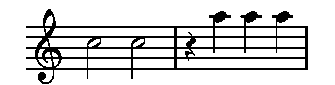
\includegraphics{hauhau.pdf}\\[-.1em]
\parbox{5cm}{\small\hspace*{10.5mm}\textit{hauhau} \hspace*{9mm} \textit{hauhauhau}\\}
\end{center}

\noindent = der Hund bellt. Ähnliches beobachten wir wohl bei den Sprechversuchen der Kinder. \sed{Der Sprachlaut aber, selbst der onomatopoetische, muss sich den Fesseln der Schallmimik entrungen haben, um wahrer Sprachlaut zu werden; er muss abstrahiren, generalisiren, denn alle Sprache, selbst die roheste, bewegt sich in Abstractionen und nennt das Einzelne mit dem Namen der Gattung.}

Wir dürfen annehmen, dass unsere Altvordern ihre Rede mit lebhaftem Gesten- und Mienenspiel begleitet, oft auch durch solche optische Mittel ersetzt \sed{{\textbar}{\textbar}312{\textbar}{\textbar}}\phantomsection\label{sp.312} oder ergänzt haben. Was führte sie nun dazu, die Stimm- und Gehörsorgane vorzugsweise und am Ende fast ausschliesslich mit dem Geschäfte der Verständigung zu betrauen?

Vor Allem wohl die Natur der Objecte selbst. Solche sind in erster Reihe die Empfindungen des Menschen, deren Ausbruch zugleich, wenn auch ungewollt, eine Aufforderung an die Mitmenschen enthält. Freude, Angst, körperlicher oder seelischer Schmerz, Schreck, Erstaunen: sie alle drängen unmittelbar zu Stimmäusserungen.

Zweitens erregt Nichts in der Aussenwelt so sehr die Aufmerksamkeit des Menschen, wie der unerwartet in’s Gehör fallende Ton und die heftige Bewegung, die auch hörbar zu sein pflegt. Nun ist der Zustand des wachen Menschen der, dass er fortwährend etwas sieht, oft aber gar nichts hört, sei es, dass innerhalb seines Gehörkreises kein Schall ertönt, sei es, dass er der leisen und \fed{der} gewohnten Geräusche, wie etwa des Summens kleiner Insecten, nicht Acht hat. Darum ist der \update{Gehörsinn}{Gehörssinn} \fed{{\textbar}303{\textbar}}\phantomsection\label{fp.303} viel mehr den heftigen Überraschungen ausgesetzt, als der Gesichtssinn, darum führt er viel öfter dem Gemüthe heftige Erregungen zu. So ist der Zuruf das beste Mittel, um die Aufmerksamkeit der Mitmenschen auf uns zu ziehen, und er ist auch da wirksam, wo uns die Blicke Anderer nicht erreichen können. Dazu kommt, dass Gesichtseindrücke gleichzeitig vielerlei, Gehörseindrücke dagegen fast immer nur Eins auf einmal zu enthalten pflegen; man sieht viele Dinge zugleich, nimmt aber in der Regel auf einmal nur einen Schall deutlich wahr. Und jeder einzelne Gegenstand zeigt eine Mehrzahl optischer Eigenschaften: Grösse, Gestalt, Farbe, Ruhe oder Bewegung irgend welcher Art, – während unter seinen möglichen akustischen Wirkungen immer nur eine besonders sinnfällig und bezeichnend sein wird.

Drittens kann der Mensch mit seinen körperlichen Mitteln die Geräusche und Töne der Aussenwelt leichter und verständlicher nachahmen, als ihre Gestalten oder gar ihre Farben. Wo freilich die akustischen Vorstellungen fehlen, da musste mit optischen Mitteln nachgeholfen werden, und dieser Zwitterzustand der Sprache wird sehr lange angedauert haben. Wir werden bald weiter verfolgen, wie er doch am Ende durch allerlei Übertragungen überwunden werden konnte. \sed{Wir dürfen aber schon jetzt von \so{symbolisirender Onomatopöie} reden. Das Thier wird mit dem Tone, den es hervorzubringen pflegt, benannt, auch wenn es schweigt. Das Brechen, Fallen, Rollen, Schneiden, Reissen u. s. w. kann mehr oder minder geräuschlos geschehen; jenes Geräusch aber, von dem es andere Male begleitet war, bleibt nun sein conventionelles Zeichen. Aber noch mehr: Das Gemüth wird von verschiedenen Gehörsempfindungen sehr verschieden erregt, – recht eigentlich gestimmt; der Körper hat, je nach der Art, wie er berührt wird, sehr verschiedene Empfindungen, die wieder in ganz bestimmter Weise auf das Gemüth wirken, und auch diese Berührungen, das Schlagen,} {\textbar}{\textbar}313{\textbar}{\textbar}\phantomsection\label{sp.313} \sed{Schütteln, Stossen, Stechen, Streicheln u. s. w., können hörbar oder unhörbar geschehen. Nun arbeitet die Sprache in Analogien: das Stumme macht sie tönend, und das Körperliche überträgt sie auf’s Gemüthliche. Sie ist eine geschickte Bildnerin und schafft in geschmeidigem Stoffe.}

\sed{Vielleicht hat auch \textsc{B. Bourdon }\corr{1901}{(L’expression}{(d’expression} des émotions et des tendences dans le langage, Paris 1892 p. 38 flg.) Recht, wenn er auf das feine Taktgefühl der Zunge hinweist und vermuthet, die Zunge bewege sich so, dass sie selbst etwas Ähnliches empfinde, wie sie mit ihren Lauten ausdrücken wolle, sie schaffe sich selbst das Gefühl des Druckes, des Gleitens, Streichelns, Kitzelns u. s. w. und erzeuge dabei entsprechende Schallwirkungen. Der Hörer brauchte dann das Gehörte nur nachzuahmen, um an der eigenen Zunge Gleiches zu empfinden. Hier wäre also die Spracherzeugung auch imitativ, aber die Nachbildung gelte dem Tastsinne, die Schallwirkung wäre nur ein begleitender Nebenumstand. Die Hypothese ist gewiss feinsinnig; schon \corr{1901}{\textsc{Byrne}}{\textsc{Byren}} hatte eine ähnliche aufgestellt; mir scheint sie mehr glänzend als einleuchtend.}

Genug, schon jetzt haben wir vom Standpunkte des strenggläubigen Darwinismus aus ein recht buntes, wenn auch nicht gerade ein liebliches Bild vom Seelen- und Sprachleben unserer Altvordern gewonnen. Und seltsam, das Beste dabei musste sehr trüben Quellen entfliessen: Neid, Langeweile, Spieltrieb, Lüge, Eitelkeit, Neugier, Geschwätzigkeit, Alles musste mitwirken, um den sprechenden Menschen zu bilden. Wohl jede seiner Eigenschaften finden wir auch bei Thieren wieder, nirgends sonst aber, die guten inbegriffen, sie alle so beisammen. Vielseitigkeit der körperlichen und seelischen Beanlagung, ihr entsprechend wechselvolle \update{Mannich\-faltigkeit}{Mannig\-faltigkeit} der Schicksale und Beschäftigungen, stets zunehmende Menge der leiblichen und geistigen Bedürfnisse: das war es, was den Menschen zum Denker und Sprecher machte. Denn Beides, Denk- und Sprachvermögen, musste hinfort, sich wechselseitig fördernd, aneinander emporranken.

\pdfbookmark[2]{§4. Laute und Töne in der Ursprache.}{IV.II.4}
\cohead{§4. Laute und Töne in der Ursprache.}
\subsection*{§. 4.}\phantomsection\label{IV.II.4}
\subsection*{Laute und Töne in der Ursprache.}

Der Gedanke liegt nahe, es müsse die Phonetik der ältesten menschlichen Sprache besonders einfach gewesen sein: wenige Vocale, – man \fed{{\textbar}304{\textbar}}\phantomsection\label{fp.304} hat wohl an die drei angeblichen Urvocale \textit{a}, \textit{i}, \textit{u} gedacht, – und sehr wenige Consonanten, etwa dieselben, die wir zuerst von kleinen Kindern hören. Ich kann dies nicht glauben; dies eine Mal scheint mir der Rückschluss von der Kindersprache auf die Ursprache verfrüht.

Der Urmensch, wenn anders das Bild, das wir vorhin von ihm zu gewinnen suchten, zutrifft, schuf nicht nur eigene Laute, sondern lauschte auch der Aussenwelt ihre Schallwirkungen ab und übte sich diese nachzuahmen. So ward die \sed{{\textbar}{\textbar}314{\textbar}{\textbar}}\phantomsection\label{sp.314} ganze Natur seine Sprachlehrerin, und sein Sprach- und Stimmorgan sehr \update{mannich\-faltig}{mannig\-faltig} gebildet. Die Zwischenstufen der Vocale, die \textit{ä}, \textit{e}, \textit{o}, \textit{ö}, \textit{ü} u.~s.~w., wurden ihm \update{geläufig;}{geläufig,} \sed{– insofern sind sie jedenfalls ebenso ursprünglich, wie die drei „Urvocale“ \textit{a}, \textit{i}, \textit{u};} das Rauschen, Zischen, Spritzen und Summen, das um ihn her ertönte, lehrte ihn die \textit{š}, \textit{s}, \textit{ž}, \textit{z} anwenden; in krachenden, rollenden und rieselnden Geräuschen sprach ihm die Natur verschiedenerlei \textit{r} und \textit{l} vor; und galt es, den Knall einer berstenden Nuss, das Schnalzen und Zirpen verschiedener Thiere nachzubilden, so musste er sich mit jenen Schnalzlauten behelfen, die noch heute in südafrikanischen Sprachen erklingen. Auch seine Singstimme hatte, jetzt brüllend, brummend oder heulend, jetzt kreischend oder näselnd, jetzt wohl auch in reineren Tönen mitzuwirken.

Ausdrucksvoll war die Intensität der Hervorbringung, bald für die innere Stimmung, bald für die Stärke des äusseren Geschehens, die freilich wieder stimmend wirkte. Noch mochten die Tenues und Mediae, vielleicht sammt ihren Aspiraten, nur Gradverschiedenheiten ausdrücken, sonst frei untereinander vertauscht werden, wie noch heute in manchen Sprachen.

Dass die Ursprache durchgängig und ausschliesslich aus \update{Einsylblern}{Einsylbern} bestanden habe, ist nicht glaublich. Schon das Kind gefällt sich in Doppelungen, und die Aussenwelt, zumal die Thierwelt, giebt uns deren in Menge zu hören. Aber auch zu Verbindungen verschiedenlautiger Sylben bot die Natur dem Menschen Vorbilder, so im Knattern und Dröhnen eines nahen Donners oder eines stürzenden Baumes und in den Rufen mancher Vögel. Andrerseits konnten auch manchmal vocallose Explosivlaute der Darstellung besser dienen, als volle Sylben. Brennendes Holz z.~B. lässt oft ein deutliches \textit{b’} vernehmen; \textit{t’} und \textit{pf’}, \textit{ph’} sind Laute des Spuckens und heftigen, blasenden Ausathmens. Wenn man an die verwandten Demonstrativlaute der meisten Sprachen denkt, so gewinnt man von den Manieren unserer Altvordern kein sonderlich anmuthiges Bild.

\fed{{\textbar}305{\textbar}}\phantomsection\label{fp.305}

Der Fortschritt aber, den das Lautwesen im Laufe der Zeit zu machen hatte, wird weniger in der Einführung und Unterscheidung neuer akustischer Mittel, als in der Ausscheidung mancher der vorhandenen bestanden haben, in einer Art natürlicher Zuchtwahl. Die gebräuchlichsten, darum bequemsten vertraten die selteneren, verdrängten sie allmählich. Mir ist leider hiefür kein besseres Beispiel zur Hand, als jenes {\ain}\textit{a}{\ain}\textit{a} der kleinen Kinder, das bedeutsam krächzend mit zwei entschiedenen {\ain}\textit{Ain} gesprochen wird. Diesen Laut haben manche Sprachen in überraschender Einhelligkeit durch das ihnen geläufigere \textit{k} \update{ersetzt.}{ersetzt,} \sed{so z. B. viele indogermanische, das Mandschu, das Syrjänische, das Tibetische, das Quechua, das Odschibwe.} Das stilisirte Lautzeichen trat an Stelle des getreuen Abbildes, ganz wie das optische Zeichen in der hieratischen Schrift gegenüber der hieroglyphischen Malerei; die Sprache entrang sich der Sklaverei ihrer Vorbilder, und eben hierin lag eine That wahrhaft menschlichen Fortschrittes. 

\sed{{\textbar}{\textbar}315{\textbar}{\textbar}}\phantomsection\label{sp.315}

Absichtlich habe ich mich auch diesmal wieder mit der flüchtigen Andeutung von Wahrscheinlichkeiten begnügt. Dichten, phantasiren kann man ja in’s Endlose. Eine leidlich erschöpfende, inductive Erforschung der Naturlaute in der Ursprache, wenn sie überhaupt je möglich werden sollte, würde genealogisch-historische Arbeiten voraussetzen, von deren Ergebnissen wir Jetztlebenden uns keine Vorstellung machen können.

\pdfbookmark[2]{§5. Die Personificirung, Beseelung und Belebung.}{IV.II.5}
\cohead{§5. Die Personificirung, Beseelung und Belebung.}
\subsection*{§. 5.}\phantomsection\label{IV.II.5}
\subsection*{Die Personificirung, Beseelung und Belebung.}

Der Mensch erkennt im Mitmenschen Seinesgleichen, beurtheilt ihn nach sich und urtheilt damit in der Regel richtig. Im Thiere erkennt er ein ihm ähnliches Wesen, sucht und findet in ihm dieselben Bedürfnisse und Leidenschaften, auch annähernd dieselben Kräfte, die ihn selbst bewegen. Auch dieselben geistigen Kräfte; darum mag Kinder und kindliche Völker die Thierfabel ganz anders anmuthen, als uns. Aber auch mit dem Pflanzenreiche und mit der ganzen Welt des Unorganischen weiss sich der Mensch bald in freundlichem bald in feindlichem Verkehre. Ob ihn ein Dorn ritzt, eine Katze krällt, oder ob ihn ein Mitmensch seine Nägel fühlen lässt: seine Empfindung ist die gleiche, – warum sollten Jene, die ihm den Schmerz verursacht, nicht auch das Gleiche beabsichtigt haben? warum sollte er dem Einen mehr zürnen, \fed{{\textbar}306{\textbar}}\phantomsection\label{fp.306} als dem Anderen? Das Kind, das sich gegen die Tischkante stösst, prügelt den Tisch: „Wart’, du böser Tisch!“ Der Tisch wird ihm ein Du, eine zweite Person, die also auch ihr Ich haben wird, ein böses, feindliches Ich. Ein liebes Spielzeug aber küsst es, und wenn es recht blank geputzt ist, freut sich das Kind gleich mit in die Seele der Sache hinein, denn es hat eben die Sache beseelt. Auch uns Erwachsenen und Gebildeten kann es, wenn wir nicht froschkühl sind, in unbewachten Momenten ähnlich ergehen. Dann lassen wir an Sachen, die uns ärgern, unsern Ärger aus, zerknicken die Feder, die nicht schreiben will, oder rufen ihr eine Verbalinjurie nach, während wir sie wegwerfen. Der Zorn thut dabei die Hauptsache; denn dem Widerspenstigen legen wir eher einen eigenen Willen unter, als dem \update{Gefügigen.}{gefügigen.} Bei rohen Völkern thut aber auch die Furcht ihr Theil. Was mir schaden kann, das kann ich vielleicht durch Bitten und Wohlthaten versöhnen, sodass es nicht mehr mir, sondern meinen Feinden, schadet, mir ein Bundesgenosse, ein Schutzgott (Fetisch) wird. Und was mir nun dient und nützt, das ist mein Freund, mit dem stelle ich mich auf Du und Du. Dieser naiven Anschauung dünkt Alles erklärlich: Alles hat sein Ich, seinen Willen, – warum sollte dieser Wille weniger launenhaft sein, als der meinige? Sagen wir doch selbst von einer Uhr oder einer Flinte, die ohne erkennbaren Grund ihren Dienst versagen: sie haben ihre Mucken. \sed{Jene unpersönlichen Verba, die} {\textbar}{\textbar}316{\textbar}{\textbar}\phantomsection\label{sp.316} \sed{bei uns die Witterungsereignisse erzählen: „es regnet, es donnert“ u. s. w. sind nichts weniger als naiv. Das Kind will wissen, \so{wer} donnert? Und ob man ihm dann antwortet: „Der liebe Gott“ oder: „Der böse Mummum“, – so ist es für’s Erste befriedigt; ihm ist jedes Geschehniss eine That. Nun weiss es auch den Thäter, – was will es mehr? Verbinden sich nun That und Thäter unlösbar, wird jedem Naturereignisse sein besonderer Urheber zugetheilt, das Nomen actoris zum Nomen proprium \corr{1901}{erhoben:}{erhaben:} so ist das Personal für einen wohlbesetzten Olymp leicht zusammengebracht.}

Kein Zweifel, diese naive Beseelung der Welt hat an der Schöpfung und Ausgestaltung der menschlichen Sprache mächtig mitgewirkt. Für menschliches Thun und Empfinden waren die Benennungen da. Indem man die Dinge vermenschlichte, ergaben sich leicht die Ausdrücke für ihre Äusserungen und darnach die Namen für sie selbst. Hier fanden die Launen einer jugendlichen Phantasie ihren breitesten Spielplan. Jeder durfte thun, was heute nur den Dichtern vergönnt ist.

Wo immer wir der Herkunft der Ausdrücke, der lexikalischen oder der grammatischen, folgen können, es handle sich um klare Zusammensetzungen oder um syntaktische, periphrastische Gebilde, überall ist der Hergang der gleiche: es sind Übertragungen, das Seelenlose wird wie ein Beseeltes, das Leblose wie ein Belebtes behandelt, und des Protagoras Wort gilt auch hier: Der Mensch ist das Mass aller Dinge. Manchmal ist es, als feierte die durchgeisterte Welt der Urmenschen in den jüngsten Sprachen ihre Auferstehung. Der Franzose lässt den Stein „milden \fed{{\textbar}307{\textbar}}\phantomsection\label{fp.307} Sinnes“, doucement, dahinrollen; und wenn es nicht gelingt, einen Nagel in die Wand zu treiben, so sagt der Engländer: „It will not hold“, und der Obersachse sagt wohl: „Es lernt nicht halten“, als fehlte es dem Nagel am guten Willen oder gar an der nöthigen Intelligenz! \sed{Dazu kommt nun das ganze Heer der sonstigen Übertragungen:}

\sed{von Sinne zu Sinne, zumal zwischen Gesicht und Gehör, z. B. helle, dunkele, tiefe Töne in der Musik und in der Malerei,}

\sed{von einem Naturreiche oder Körper zum anderen, z.~B. malaisch \textit{māta hāri}, Auge des Tages = Sonne, \textit{māta āyer}, Auge des Wassers = Brunnen, \textit{ānaq pōhon}, Kind des Baumes = Strauch, \textit{ānaq māta}, Kind des Auges = Augapfel,}

\sed{von Körperlichem auf Geistiges: eiserne Stirn = Frechheit, feine Nase = Spürsinn. – Ähnliches und vielleicht noch Stärkeres darf man auch der Phantasie des Urmenschen zutrauen.}

Der Spielraum ist unendlich weit, der Wege sind unzählbar viele. Und doch sollte man meinen, auch was wie Laune und Willkür scheint, müsse seine Gesetze haben. Man kann ja Alles vergleichen, was irgend Ähnlichkeiten bietet. Aber nicht alle Vergleiche sind gleich gut, und unter den guten finden die gleichwerthigen nicht allemal gleichmässig Anklang. Die Ähnlichkeit muss sofort \sed{{\textbar}{\textbar}317{\textbar}{\textbar}}\phantomsection\label{sp.317} einleuchten: darin besteht die Güte des Vergleiches. Und das Vergleichsbild muss dem Kreise unseres gewöhnlichen Denkens entlehnt sein: darauf beruht sein Anspruch auf Volksthümlichkeit, das heisst auf dauernden Platz im Sprachgute. So müsste die Etymologie der Wörter und Wortformen von der Sinnes- und Lebensweise der alten Völker zeugen, – wenn sie nur etwas deutlicher reden wollte.

In der That würde sie dann noch von ganz anderen Dingen erzählen. Denn nicht nur das Mass, sondern auch der Mittelpunkt der Welt ist der Mensch, dünkt sich es zu sein. Alles dreht sich um ihn, bewegt sich nach ihm hin oder von ihm weg; was über ihm ist, ist oben, was hinter ihm liegt, ist hinten, und um ihn herum zieht sich der Kreis dessen, was er sein nennt und scharfen Blickes unterscheidet, – jenseits in immer weiteren, immer nebelhafteren Kreisen, das Andere, Fremde, das er, je ferner es ihm steht, um so unbestimmter erschaut und benennt. Die Anfänge der Mensehheitsgeschichte müssten sich in der Etymologie spiegeln, wenn es je gelänge, diesen Spiegel von den ihn überlagernden vieltausendjährigen Staubschichten zu säubern. Doch darauf kommt es für jetzt nicht an, nicht auf das Bild, das die Alten gemalt haben, sondern auf den Malkasten, dem sie ihre Farben entnahmen. Wie sie nun weiter die empfangenen Eindrücke von Sinne zu Sinne übertragen mochten, dafür liefern uns die heutigen Sprachen Beispiele die Hülle und Fülle.

\fed{{\textbar}308{\textbar}}\phantomsection\label{fp.308}

\pdfbookmark[1]{III. Capitel.}{IV.III.Capitel}
\cehead{{{\large IV,}} III. Inhalt und Form der Rede.}
\pdfbookmark[2]{I. Die Rede.}{IV.III.I}
\cohead{I. Die Rede.}
\section*{III. Capitel.}\phantomsection\label{IV.III}
\section*{Inhalt und Form der Rede.}
\subsection*{I.}\phantomsection\label{IV.III.I}
\subsection*{Die Rede.}
Sprache ist Rede, ist Ausdruck des Gedankens, ist Satz. Wir fragen zunächst nach dem Inhalte der Rede: Welcher Art Gedanke wird ausgedrückt, welcher Art ist also die Rede, der Satz?

Wir müssen hier wieder etwas weiter ausholen. Denken heisst Vorstellungen verknüpfen. Die Eintheilung der Vorstellungen in Anschauungen und Begriffe überlassen wir vorläufig der Philosophie. Die Rede ist Ausdruck jener Verknüpfung von Vorstellungen, also Ausdruck sowohl der zu verknüpfenden Vorstellungen, als auch ihrer Verknüpfung, mag diese Verknüpfung noch so lose, ihr Ausdruck noch so schwächlich sein.

\largerpage
Wollten wir hierbei stehen bleiben, von diesem Standpunkte aus die Arten der Rede zu classificiren versuchen, so wüsste ich keinen anderen Eintheilungs\-\sed{{\textbar}{\textbar}318{\textbar}{\textbar}}\phantomsection\label{sp.318}grund, als jene verschiedenen Verknüpfungsweisen: ob thatsächlich, möglich, nothwendig, gewiss, gewollt u.~s.~w. Dann würden also die Sätze:

~~~~Du kommst,

~~~~Du sollst kommen,

~~~~Du kannst kommen, 

~~~~Du musst kommen, 

~~~~Du kommst hoffentlich, 

~~~~Du kommst wahrscheinlich, 

\largerpage[-1]\noindent ebensoviele verschiedene Formen der Rede darstellen.

Offenbar \update{thuen}{thun} sie dies nicht; der Standpunkt, von dem aus wir die Eintheilung versuchten, war verfrüht. Worin lag nun der Fehler? Darin, dass wir nur an das redende Ich dachten, nicht auch an das angeredete Du. Ein solches ist entweder vorhanden oder nicht vorhanden. Nicht vorhanden ist es nur im Falle des eigentlichen Ausrufes. Sonst ist es überall, mindestens im Geiste des Redenden, gegenwärtig, die Rede ist im weiteren Sinne Gedankenmittheilung, mag ich nun den Angeredeten in ein Wir mit einschliessen, mag ich mir im Selbstgespräche mich selbst \fed{{\textbar}309{\textbar}}\phantomsection\label{fp.309} wie im Spiegelbilde gegenüberstellen. Wir wollen zunächst die mittheilende Rede in diesem weiteren Verstande in’s Auge fassen. Denn die folgenden Untersuchungen werden uns in ein wirres Gebiet führen, und es ist gut, da anzufangen, wo noch die Dinge am Klarsten zu liegen scheinen.

Nun enthält jede Rede unmittelbar eine Aufforderung an das Du: „Höre mich!“ Bekanntlich giebt man in manchen Gegenden und Sprachen dieser Aufforderung noch besonderen Aus- und Nachdruck. „Höre, – \textit{écoutez}.“

Verlange ich nichts weiter als Aufmerksamkeit, so ist meine Rede \so{Declamation} im weiteren Sinne des Wortes. Dann stelle ich mir aber unter dem Du jemand anderes vor, als meine Zuhörerschaft, und an dies Du stelle ich noch andere Anforderungen. Wende ich mich aber an die Zuhörerschaft, wird die Declamation zur Ansprache, so stehen wir wieder auf dem alten Punkte: ich verlange von den Angeredeten noch etwas mehr als blosse Aufmerksamkeit. Um dieses Mehrere wird es sich hier handeln.

\phantomsection\label{IV.III.I.1}1. Ich spreche meinen Gedanken aus und verlange, dass der Angeredete nun ebenso denke: „Glaube mir!“ Die entsprechende Form der Rede ist die \so{mit\-thei\-lende im engeren Sinne}: ich theile Dir meinen Gedanken mit, damit er hinfort auch Dein Gedanke werde.

\phantomsection\label{IV.III.I.2}2. Ich kann Dir nichts mittheilen, was ich nicht habe oder zu haben vorgebe. Du kannst mir nichts glauben, was ich nicht – mindestens vorgeblich – glaube oder weiss. Bin ich aber selbst im Ungewissen, so kannst Du vielleicht mir mit\-theilen, was mir fehlt. Nun begehre ich dies von Dir: „Sage \sed{{\textbar}{\textbar}319{\textbar}{\textbar}}\phantomsection\label{sp.319} mir...!“ Die dem entsprechende Redeform ist die \so{fragende}. Die antwortende dagegen ist ihrer Natur nach nur eine Unterart der mittheilenden.

\phantomsection\label{IV.III.I.3}3. Ich will weder, dass Du etwas durch mich erfahrest, noch dass ich etwas durch Dich erfahre, sondern dass Du etwas, gleichviel was, thuest oder unterlassest Die Form dieser Rede nennen wir die \so{gebietende} (verbietende, bittende, verbittende).

\largerpage
\phantomsection\label{IV.III.I.4}4. Die menschliche Sprache ist ihrem Wesen nach Verkehrsmittel; dass dem Redenden ein Du mindestens im Geiste gegenwärtig sei, bildet die Regel. Allein ebenso ist es die Regel, dass ich nicht nur Dir etwas sagen, sondern auch mich aussprechen will; ich will selbst hören, was ich denke, und wie ich empfinde. In solchen Stimmungen befindet sich \fed{{\textbar}310{\textbar}}\phantomsection\label{fp.310} der Mensch unter dem Einflusse mächtiger Erregungen, die nach Entladung drängen. Was er zu dem Ende thut, ist im weiteren Sinne pathologisch, es sei Weinen, Lachen, Händeklatschen, Aufstampfen mit dem Fusse, ein Aufschrei, ein Schnalzen mit der Zunge oder ein Stück menschlicher Rede. Denn auch die Sprache ist uns durch Übung so zur Natur geworden, dass sie unbewusst und absichtslos aus unserm Innern hervorbrechen kann. Solche Reden nun nennen wir \so{ausrufende}. Wir mussten ihrer besonders gedenken, zunächst weil sie in der That auf anderer seelischer Grundlage beruhen, als jene, welche dem Verkehre dienen; dann aber auch, weil es nahe liegt, dass sich die Sprache, wo sie die Fesseln des Verkehres abgestreift, neue Formen geschaffen habe.

\label{IV.III.I.5}Jetzt gilt es, die gewonnene Eintheilung auf ihre Durchschlägigkeit und Vollständigkeit zu prüfen, und da erstehen auf den ersten Blick ernstliche Bedenken, die beseitigt werden müssen.

A. Wir haben uns an die herkömmlichen Benennungen gehalten, der mittheilenden Rede die fragende und die befehlende entgegengesetzt, die doch in Wahrheit auch einen Gedanken des Redenden mittheilen sollen.

B. Wir haben die fragende Rede der befehlenden nebengeordnet. Der Befehl verlangt vom Angeredeten eine positive oder negative Thatäusserung: Thue das, unterlasse jenes! Eine solche Thatäusserung ist aber doch auch die Antwort, zu der der Gefragte aufgefordert wird. Also könnte es scheinen, als wäre die Frage nur eine Unterart des Befehles.

C. Endlich kleidet die Sprache oft ihre Gedanken in geborgte Gewänder. Die \so{mittheilende} Redeform mag jetzt eine Frage enthalten: „Ich wüsste gern ob ...“, – jetzt mag sie einen Befehl, eine Bitte, ein Verbot in sich schliessen: „Du musst ..., Du darfst nicht ..., Du würdest mir einen Gefallen \update{thuen,}{thun,} wenn Du ...“ u.~s.~w. Die fragende Form mag ein fertiges Urtheil verhüllen. Es ist dies der Fall der rhetorischen Frage, die besagen will: „Gieb die Antwort nicht mir, sondern Dir, stelle Dir die Frage, so wirst Du urtheilen wie ich!“ Oder es mag eine Aufforderung in fragender Form ausgesprochen werden. „Wirst \sed{{\textbar}{\textbar}320{\textbar}{\textbar}}\phantomsection\label{sp.320} Du gleich kommen?! Wärest Du wohl so freundlich ...?“ Es scheint naturgemäss, dass auch der Ausruf gern die fragende Form annehme: „Wie schön ist das!“ Denn der Zustand der Gemüthserregung ist jenem des unfertigen Urtheils verwandt. Die \so{befehlende} und \so{bittende} Form eignet sich ohne Weiteres da, wo Auskunft erfordert wird: \fed{{\textbar}311{\textbar}}\phantomsection\label{fp.311} „Nenne mir Deine \update{Gehülfen!}{Gehilfen!} Sagen Sie mir doch die genaue Zeit!“ Endlich kann der Ausruf jetzt eine thatsächliche Mittheilung bezwecken: „Ein schönes Bild!“, – jetzt eine Frage: „Wüsste ich doch ...!“ – jetzt wohl auch eine Aufforderung: „Wenn Du mir doch hülfest!“ 

Wir halten uns an die Formen und stellen nun der ausrufenden die drei übrigen als mittheilende im weiteren Sinne gegenüber.

Der mitzutheilende Gedanke kann sein ein Urtheil, ein Wunsch, oder \update{beides}{Beides} zugleich.

Er sei ein Urtheil, so kann dieses vollständig oder unvollständig sein. Ist es vollständig, so ist die Rede \so{mittheilend im engeren Sinne des Wortes}.

Ist das Urtheil unvollständig, so theile ich es dir als unvollständiges mit, um es von dir ergänzen zu lassen. Beides, jene Mittheilung eines Urtheils und jener ausgesprochene Wunsch nach dessen Vervollständigung, vereinigt sich in der \so{Frage}.

Endlich: der Gedanke sei vollständig, aber er sei nicht ein Urtheil, sondern ein Wunsch, dessen Erfüllung ich von dir begehre: so sind die Voraussetzungen gegeben zur \so{befehlenden} Rede und ihren Verwandten: der bittenden, \update{verbittenden,}{verbietenden,} rathenden u.~s.~w.

Zur Übersicht stellen wir für die drei mittheilenden Redeformen folgendes Schema auf:

\begin{table}[h]
\centering
\begin{tabular}{c c c c c c}
& \multicolumn{3}{c}{Der mitzutheilende Gedanke ist} \\
\multicolumn{1}{l}{\hspace*{.7cm}\tikzmark{urteil}{ }} & & & &
\multicolumn{1}{r}{\tikzmark{wunsch}{ }\hspace*{1cm}} & \\
\multicolumn{2}{c}{A. ein Urtheil. Dies ist} & & \multicolumn{2}{c}{B. ein Wunsch} \\
\multicolumn{1}{l}{\tikzmark{vollstaendig}{ }} & \multicolumn{1}{r}{\tikzmark{unvollstaendig}{ }} & & \multicolumn{2}{l}{\pushbar} \\
\multicolumn{1}{l}{a) vollständig} & \multicolumn{1}{r}{b) unvollständig} & & \multicolumn{2}{l}{\pushbar} \\
\LARGE {\textbar} & \multicolumn{2}{c}{ \LARGE {\textbar} } & \multicolumn{2}{l}{\pushbar} \\
\LARGE {\textbar} & \multicolumn{2}{l}{\tikzmark{frage}{ }} & \multicolumn{2}{r}{\tikzmark{befehl}{ }} \\
\multicolumn{1}{l}{1. Mittheilung} & \multicolumn{2}{c}{2. Frage} & & \multicolumn{1}{r}{3. Befehl u.~s.~w.}
\end{tabular}
\end{table}

\tikz[overlay,remember picture] {

\draw[style={decorate,decoration={brace}}, thick] (urteil) -- (wunsch) node {};

\draw[style={decorate,decoration={brace}}, thick] (vollstaendig) -- (unvollstaendig) node {};

\draw[style={decorate,decoration={brace,aspect=0.62}}, thick] (frage) -- (befehl) node {};
}

Ich glaube, diese Tabelle trägt die Gewähr der Vollständigkeit in sich, und sie wird noch ein zweites Mal analog anwendbar sein, wenn es gilt, die \so{ausrufende} Rede in Unterarten zu theilen.

Unterscheiden wir auch hier wieder zwischen Inhalt und Form.

Der Form nach kann der Ausruf sein:

\phantomsection\label{IV.III.I.A}A. ein vollständiger Satz \update{bez.}{bezw.} ein Satzwort, z. B. ein optativer: „Käme er doch!“ oder ein fragender. „Wie schön ist das!“ Ein Imperativ: „Halt!“ An die besonderen modalen Verbalformen oder \update{Hülfswörter,}{Hilfswörter,} die in manchen Sprachen der ausrufenden Rede \retro{dienen,}{dienen;} mag hier nur im Vorübergehen erinnert werden.

\fed{{\textbar}312{\textbar}}\phantomsection\label{fp.312} \sed{{\textbar}{\textbar}321{\textbar}{\textbar}}\phantomsection\label{sp.321}

\phantomsection\label{IV.III.I.B}B. Elliptisch, einen Satz ersetzend, z. B. „Brav gemacht!“ „Abgeblitzt!“ „Schon wieder Einer!“ Manchmal werden wohl solche Ellipsen durch einen nachträglichen Zusatz ergänzt zu vollständigen Sätzen, und dann mag sich der seelische Hergang in einer eigenartigen Anordnung der Satzglieder ausprägen: „Schon wieder Einer – kommt da an!“ „Ein wunderlicher Mensch, – ist NN.“ So finden wir im Chinesischen: \textit{šén tsāi!} Gut, traun! Aber auch, mit nachträglicher Nennung des Subjectes: \textit{šén tsāi wén}, gut, traun, (war deine) Frage! Wir reden dann von Inversionen, müssen aber bedenken, dass diese nicht, wie rechtschaffene Sätze, in der Seele fertig vorher geformt waren, sondern erst hinterdrein, so zu sagen durch einen späteren Anbau, zu einem Ganzen geworden sind. – Die beiden bisherigen Formen sind wohl ausrufend und werden auch von den Zuhörern so aufgefasst. In der That pflegen aber solche Ausrufe nur dann über unsere Lippen zu kommen, wenn wir wissen, dass man uns hört, und wollen, dass man uns höre. So könnte es scheinen, als wären sie doch im weiteren Sinne mittheilend. Ich denke indessen daran, wie oft uns derlei Ausrufe auf den Lippen schweben und ungeäussert bleiben, unterdrückt werden. Warum das? Weil es doch zu nichts frommen würde, sie verlauten zu lassen. Sprechen wir sie Dritten gegenüber aus, so ist der Thatbestand dieser: Wir bezwecken eine Mittheilung, machen diese aber in solcher Form, als sprächen wir lediglich mit der Absicht, unserer übervollen Seele ein Ventil zu öffnen. Man sagt wohl: „Es musste heraus, ich musste mich aussprechen“, und dann empfindet man es als eine doppelte Erleichterung, wenn nun Andere in Mitleidenschaft gezogen werden. – Imperative wie: „Hut ab!“ „Still gestanden!“ sind Zurufe, also Mittheilungen im weiteren Sinne des Wortes, nicht Ausrufe.

\largerpage[-2]\phantomsection\label{IV.III.I.C}C. Vocative im weiteren Verstande des Wortes, ich möchte sagen in zweiter und dritter Person, sind absolute, der Satzverknüpfung entbehrende substantivische Redetheile, die sich aber nicht an eine vorhandene oder vorgestellte zweite Person richten. Dahin gehören in vielen Fällen die Anrufungen übersinnlicher Mächte oder fürchterlicher Ereignisse, z.~B. „Herr Gott!“ „Den Teufel!“ „Donnerwetter!“ „Schwere \update{Noth.“}{Noth“.} Es sind das Stimmungsäusserungen, mit denen keinerlei Gebet oder Beschwörung beabsichtigt wird: man denkt an gar keine zweite Person. Auch pflegt man bei solchen Ausrufen nicht an etwaige Zuhörer zu denken. Das unterscheidet sie von jenen Vocativen und sonstigen \fed{{\textbar}313{\textbar}}\phantomsection\label{fp.313} Zurufen, die an ein Du gerichtet sind: Polizei! Hülfe! Feuer! Diese sind im weiteren Sinne mittheilend. – Ob der interjectionelle Accusativ im Lateinischen, z. B. \fed{Me} miserum! hierher oder unter die Ellipsen gehört, wage ich nicht zu \update{entscheiden.}{unterscheiden.}

\phantomsection\label{IV.III.I.D}D. Reine Interjectionen, das heisst Wörter, die keinem anderen Redetheile angehören. Sie dürften einzutheilen sein

\phantomsection\label{IV.III.I.a}a) in mehr objective, nachahmende, z.~B. Pardauz! hopsa! puff!

\phantomsection\label{IV.III.I.b}b) in mehr subjective, d.~h. solche, die nur ein individuelles Empfinden, \sed{{\textbar}{\textbar}322{\textbar}{\textbar}}\phantomsection\label{sp.322} Schmerz, Freude, Erstaunen u.~dgl. ausdrücken: Au! Ei! Ach! Hm! Es sind dies ungeformte Wörter, die der geformten Sprache gegenüber auch in lautlicher Hinsicht eine Ausnahmestellung einnehmen können. In ihnen hat das Hochdeutsche noch anlautende \textit{p}, haben Dialekte, die sonst \textit{ö} und \textit{ü} in \textit{e} und \textit{i} verwandeln, diese Laute rein bewahrt. In beiden Hinsichten stehen ihnen gewisse Auf- und Zurufwörter gleich, z.~B. das Hö und Hüist der Fuhrleute und Ackerknechte in Sachsen, das Ruhe gebietende St! Auch das fragende Hm? ist hierher zu rechnen, und gewiss ursprünglich auch die Deutelaute, die den Demonstrativpronominibus zu Grunde liegen mögen. Solche „Naturlaute“, wie man sie wohl genannt hat, mögen zuweilen verstümmelte oder unverstandene ältere organische Gebilde in sich enthalten. Unser Jemine! ist wohl ein Ersatz für den Namen Jesus, vielleicht mit Anklang an \textit{domine}. In Spanien ruft man arglos: \textit{Caramba!} statt des unfläthigen \textit{carajo}, wie man in manchen Gegenden Deutschlands Gottstrambach oder ’strambach statt Gott straf’ mich sagt. Umgekehrt können jene Laute als Wurzeln oder Stämme grammatische Formung erfahren. Man sagt: die Katze miaut (maunzt), le chat miaule. Von ach! und pfui! bilden wir \retro{ächzen}{ächsen} und (mundartlich) pfuzen, ganz wie duzen und siezen von Du und Sie. Dass Thiere nach ihren Rufen benannt werden, ist wohl allgemein verbreitet. Der Kukuk hat selbst dafür gesorgt, dass die germanische Lautverschiebung seinem Namen nichts anhaben konnte. Von jenen Onomatopöien aber, die in die Urgeschichte der Sprache fallen, brauchen wir hier nicht wieder zu reden. 

\largerpage[-2]\phantomsection\label{IV.III.I.6}Mit Obigem sind meines Wissens die möglichen Formen der ausrufenden Rede erschöpft. In der That die möglichen Formen der menschlichen Rede überhaupt. Diese ist entweder grammatisch geformt oder ungeformt. Die geformte ist entweder ein vollständiger Satz oder kein vollständiger Satz. Letzteren Falles ist sie entweder ein zur Ergänzung aufforderndes Bruchstück eines Satzes – elliptisch, – oder sie lehnt \fed{{\textbar}314{\textbar}}\phantomsection\label{fp.314} die syntaktische Verknüpfung formell ab, ist absolut. Die vierte Kategorie, jene der ungeformten Sprachäusserungen, theilten wir so, dass die Eintheilung zugleich den Ursprung und den Inhalt betraf. Soll sie nun auch auf die mittheilenden Sprachäusserungen bezogen werden, so gerathen wir in Schwierigkeiten, die wir besser noch vermeiden. Wir fassen aber das bisher Gewonnene in ein Schema zusammen.

\begin{table}[h]
\centering
\tabcolsep=0.5cm
\begin{tabular}{l r l}
\multicolumn{3}{c}{Der sprachliche Ausdruck ist} \\
\tikzmark{geformt}{ } & & \multicolumn{1}{r}{\tikzmark{ungeformt}{ }\hspace*{1cm}} \\
\multicolumn{1}{c}{A. grammatisch geformt} & & \multicolumn{1}{c}{B. ungeformt} \\
\tikzmark{vollersatz}{ } & \tikzmark{absolut}{ } & \multicolumn{1}{c}{\LARGE {\textbar}} \\
\multicolumn{2}{c}{a) voller Satz, b) Ellipse, c) absolut,} & a) nachahmend, \\
& & b) Empfindungen äussernd, \\
& & c) deutend, \\
& & d) fragend . . .
\end{tabular}
\end{table}

\tikz[overlay,remember picture] {

\draw[style={decorate,decoration={brace}}, thick] (geformt) -- (ungeformt) node {};

\draw[style={decorate,decoration={brace}}, thick] (vollersatz) -- (absolut) node {};
}

\sed{{\textbar}{\textbar}323{\textbar}{\textbar}}\phantomsection\label{sp.323}

\noindent Nun aber, da wir die im weiteren Sinne mittheilende Rede mit in Betracht ziehen, müssen wir auch den Begriff der Ellipse ausdehnen auf jederlei eigentliches Satzfragment, auch auf den Fall, wo im Zwiegespräche die Ergänzung zum Satze aus der Rede des Anderen zu erholen ist, \retro{z.~B.}{z.~B,} Wer war dort? – Ich (war dort). – Wann (warst Du dort)? – Gestern. – Nun? Und ... ? (was geschah da?)

Jetzt kehren wir zur ausrufenden Rede zurück, um ihren möglichen Inhalt zu untersuchen.

Im Ausrufe äussert sich eine lebhafte Erregung, entweder nur die Art dieser Erregung, oder auch ihr Grund. Der Grund kann sein ein Wunsch oder eine vollendete Thatsache. Ist er eine solche, so kann die Erregung entweder in dem bekannten Theile der Thatsache, oder darin beruhen, dass wir einen Theil der Thatsache nicht kennen. Das Schema, das wieder den Eindruck der Vollständigkeit machen würde, gestaltet sich demnach folgendermassen :

\begin{table}
\begin{tabular}{c r r r}
\multicolumn{3}{c}{Äusserung der Erregung, und zwar} \\
\multicolumn{1}{l}{\tikzmark{art}{ }} & & \multicolumn{1}{r}{\tikzmark{grund}} \\
\multicolumn{1}{l}{A. nur ihrer Art nach,} & \multicolumn{2}{c}{B. auch ihrem Grunde nach} \\
 & \multicolumn{1}{l}{\tikzmark{wunsch}{ }} & \multicolumn{1}{r}{\tikzmark{tatsache}{ }} \\
 & \multicolumn{1}{r}{a) Wunsch,} & \multicolumn{1}{r}{b) Thatsache,} \\
 & \multicolumn{1}{r}{\tikzmark{alpha}{ }} & & \multicolumn{1}{r}{\tikzmark{beta}{ }} \\
 & & \multicolumn{2}{l}{α) Bekanntes, β) Unbekanntes.}
\end{tabular}
\end{table}

\tikz[overlay,remember picture] {

\draw[style={decorate,decoration={brace}}, thick] (art) -- (grund) node {};

\draw[style={decorate,decoration={brace}}, thick] (wunsch) -- (tatsache) node {};

\draw[style={decorate,decoration={brace}}, thick] (alpha) -- (beta) node {};
}

\clearpage
Setzen wir hier Thatsache und Urtheil auf eine Stufe, so ist die Analogie mit dem ersten Schema einleuchtend: Es laufen parallel: 

\ I. Wunsch – Befehl u.~s.~w.

II. Thatsache – Urtheil. 

\fed{{\textbar}315{\textbar}}\phantomsection\label{fp.315}

\ \ a) Bekanntes – Mittheilung. 

\ \ b) Unbekanntes – Frage.

Mag ich nun meine Erfahrungen mustern, mag ich versuchen, der Sache auf apriorischem Wege beizukommen, so finde ich weder die Möglichkeit zu einem neuen Schema noch zu einer Ergänzung in einem der vorhandenen Schemata, ich finde weder einen weiteren Eintheilungsgrund, noch eine Lücke in den gemachten Eintheilungen. Täusche ich mich hierin nicht, so wäre also die logische Aufgabe gelöst, und nun könnte es scheinen, als wäre ein Mittel gefunden, um jederlei Rede mit Leichtigkeit zu classificiren.

So einfach liegen indessen die Dinge nicht. Wir befinden uns nicht auf dem glattgefegten Boden der Logik, sondern mitten drinnen in dem üppigen Gewirre psychologischer Möglichkeiten. Da sind wie in einem Urwalde die Wurzeln und Gezweige der verschiedensten Pflanzen ineinander verfitzt, und Schlinggewächse ranken von Stamme zu Stamme. Jene dendrologischen Gärten aber, wo die Pflanzen säuberlich nach Arten und Unterarten in Beete und Reihen geordnet sind, sind recht eigentlich die Stätten, wo man den Wald vor lauter \sed{{\textbar}{\textbar}324{\textbar}{\textbar}}\phantomsection\label{sp.324} Bäumen nicht sieht. Und die Menschenseele schaltet schrankenloser als die schaffende Natur; vor keiner Zwitterform scheut sie zurück. Wir in \update{unserem}{unserm} Falle müssen darauf gefasst sein, jetzt die eine oder andere mittheilende Redeweise in ausrufendem Sinne, jetzt diese oder jene Art des Ausrufes statt der Mittheilung, der Frage oder des Befehles angewandt zu sehen. Es ist denkbar, dass im Leben einer Sprache die ausrufenden Redeformen die mittheilenden geradezu verdrängen, \update{ersetzen, und}{ersetzen. Und} so mag in vielen Fällen die Kunst der Classification überhaupt versagen, weil der seelische Thatbestand nicht festzustellen ist, vielleicht weil er an sich ein unsicherer, gemischter war. Stufen, Stationen konnten wir zeichnen, die möglichen Combinationen können wir zur Noth ausrechnen, aber alle Punkte einer Linie zu zählen, wäre vergebliches Bemühen.

Fruchtlos aber war die Untersuchung, wenn anders sie gelungen, darum doch nicht. Sie hat zur Entwickelung einer Reihe von Begriffen geführt, mit denen die Sprachwissenschaft fort und fort hantiren muss.

\fed{{\textbar}316{\textbar}}\phantomsection\label{fp.316}

\pdfbookmark[2]{II. §. 1. A. Der Stoff.}{IV.III.II.1}
\cohead{II. §. 1. A. Der Stoff.}
\section*{II.}\phantomsection\label{IV.III.II.1}
\othersrc{{\textbar}185{\textbar}}

\othersrc{Herr \textit{v. d. Gabelentz} sprach über \textit{Stoff und Form in der Sprache}.
\begin{center}
\so{Vorbemerkung.}
\end{center}
Die folgende Abhandlung ist bestimmt, als Capitel eines grösseren Werkes zu erscheinen, dessen Abschluss ich noch nicht absehen kann. Der Gegenstand den sie bespricht, gehört zu den vielumstrittenen, und die Streitfrage ist recht eigentlich eine grundsätzliche. Meine Anschauungen aber weichen von denen hervorragender Vorgänger und Zeitgenossen erheblich ab, und ich habe geglaubt, sie lieber selbständig entwickeln, als zu einer Polemik ausspinnen zu sollen.} 

\section*{Eintheilung der Rede in Stoff und Form.}
\subsection*{\fed{§. 1.}}
\subsection*{A. Der Stoff.}

Wir halten uns \fed{nun} an die specifisch menschliche Sprache, das heisst an diejenige, in welcher der Gedanke gegliederten Ausdruck findet, und fragen: \arbup{1901}{gray}{worin}{Worin} besteht deren Stoff? Die Antwort giebt sich von selbst: in Allem was des Menschen Denken erregt. Was \arbup{1889}{lsDarkBlue}{Alles}{alles} dies sein kann, braucht hier nicht weiter erörtert zu werden. \arbup{1901}{gray}{Uns}{Und} ist es für jetzt gleichgültig, ob der auszudrückende Gedanke eine fertige, eingebildete, erwartete oder gewollte Thatsache, eine innere oder äussere, eine Schlussfolgerung oder was immer enthält. Darauf kommt es uns an, wie er seinen Stoff gliedert.

Um ihn zu gliedern, muss er ihn zunächst zerlegen, dann wieder verbinden. Stoff lässt sich nur in Stoff zerlegen, nur in der Verbindung formen; die Formung ist ausschliessliches Erzeugniss der Verbindung, und die Verbindung dient ausschliesslich dem Zwecke der Formung. Unter Verbindung aber haben wir sowohl die blosse Aneinanderfügung als auch die gegenseitige Durchdringung zu verstehen, denn \arbup{1889 und 1891}{lsLightWine}{Beide}{beide} sind Mittel der \othersrc{{\textbar}186{\textbar}} Formung. Allein, dies sei schon jetzt bemerkt, – nicht immer dient die Formung dem Zwecke der Zergliederung und Verknüpfung, sie kann auch den Einzelstoff für sich bearbeiten, – man denke an unsere Diminutiven und, als Beispiele der Durchdringung von Stoff und Form, an die dialektischen Ausdrücke Kietze = Kätzchen, Zicke = kleine Ziege. Mit Formungen dieser Art haben wir es jetzt noch nicht zu thun.

\sed{{\textbar}{\textbar}325{\textbar}{\textbar}}\phantomsection\label{sp.325}

Nun müssen wir daran denken, dass allerdings in der Regel der Gedanke mit Einem Schlage wie ein fertiges Bild vor uns steht. Ich sage: in der Regel; denn es giebt Ausnahmen, wo uns die Bestandtheile des Gedankens Stück für Stück kommen. Jedenfalls steht der Gedanke fertig und ganz vor unserer Seele, ehe er in der Rede zum Ausdrucke kommt; und wenn ich etwa, zögernd innehaltend, sage: „Sechs mal siebzehn ist ... hundertundzwei“, so hat mir doch von Anfang an die Idee eines noch zu bestimmenden \arbup{1889}{lsDarkBlue}{Productes}{Produktes} vorgeschwebt, und der Gedanke war mithin formell vollständig. In dieser ursprünglichen Ganz\-\fed{{\textbar}317{\textbar}}\phantomsection\label{fp.317}heit wollen wir ihn eine Vorstellung (Gesammtvorstellung) nennen. Ihn in seine Bestandtheile zu zerlegen und diese Theile zum Wiederaufbaue zu verbinden ist Sache des redebildenden Denkens. Nur mit diesen Bestand\-theilen haben wir es hier zu thun: wir wollen sie Einzelvorstellungen nennen im Gegensatze zu jener Gesammtvorstellung, die das Denken zerlegend zu bearbeiten hatte. Wir begreifen den Unterschied \arbup{1889 und 1891}{lsLightWine}{Beider}{beider} nur in diesem Sinne. Ihrem Inhalte nach kann eine Gesammtvorstellung ganz einfach sein, z.~B. die eines Blitzes, – und eine Einzelvorstellung kann sehr vieltheilig sein, z.~B. die eines Krieges. So begründet auch die grössere oder geringere Bestimmtheit des Inhaltes keinen Unterschied: Caesar’s Tod und der Satz, dass das Ganze gleich ist der Gesammtheit seiner Theile: Beide können Gesammtvorstellungen \arbup{1889}{lsDarkBlue}{sein;}{sein:} Caesar aber sowohl als Tod, Gesammtheit, Ganzes und Theil sind Einzelvorstellungen.

Nun ist es die Gesammtheit seiner Einzelvorstellungen, die ein Volk in seiner Sprache darstellend zu verarbeiten hat, es ist seine Welt, die es in der Sprache zerlegt und wieder aufbaut. Es zerlegt sie in Stoffe, baut sie auf in Formen. Beides ist bestimmt durch die Eigenart des Volkes, die ihrerseits bestimmt wird durch seine innere Beanlagung und seine äusseren Schicksale. Man redet mit Recht von geistigem Standpunkte, geistiger \othersrc{{\textbar}187{\textbar}} Perspective und geistigem Horizonte. Wie in der Optik bedingt der erste die beiden anderen: \arbup{1889}{lsDarkBlue}{so viel}{soviel} oder so wenig fällt innerhalb meines Gesichtskreises, bildet meine Welt; dies steht mir am \arbup{1889 und 1891}{lsLightWine}{Nächsten,}{nächsten,} jenes ist mir in nebelhafte Ferne gerückt. Aber auch mein Auge, das geistige wie das leibliche, ist mit entscheidend: ich kann kurzsichtig sein, oder fernsichtig, vielleicht \arbup{1889}{lsDarkBlue}{farbenblind;}{farbenblind,} mein Blick mag sich besser zum \arbup{1889}{lsDarkBlue}{Über\-schauen}{Ueber\-schauen} grosser Bildflächen als zur Prüfung enger Einzelheiten eignen, er mag durch \arbup{1889}{lsDarkBlue}{Übung}{Uebung} für das Eine geschärft, durch Vernachlässigung für Anderes abgestumpft sein.

Nun sieht aber das geistige Auge mehr als das leibliche. Mit mehr oder minderer Schärfe erkennt und unterscheidet es auch die Beziehungen der materiellen Einze1vorstellungen untereinander, z.~B. zwischen dem Baume und dem Hause das „und“ oder „neben“, zwischen dem Pferde und seiner Mähne die Zugehörigkeit. Und je nach dem \arbup{1889}{lsDarkBlue}{Masse}{Maasse} und der Richtung, in der dies geschieht, drängen auch solche Kategorien zur sprachlichen Darstellung. Insoweit sind auch sie in der \sed{{\textbar}{\textbar}326{\textbar}{\textbar}}\phantomsection\label{sp.326} Regel für den sprachschaffenden Geist zunächst nicht Formen, sondern zu formender \fed{{\textbar}318{\textbar}}\phantomsection\label{fp.318} Stoff. Von ursprünglichen Formen möchte ich nur da reden, wo das Wort (der Stamm) selbst in seinem lautlichen Bestande verändert wird, durch Doppelung oder durch inneren Wandel, wie etwa in den semitischen Sprachen, im Verbum des Tibetischen und des Grebo, vorausgesetzt noch immer, dass Solches nicht mechanische Nachwirkung verschwundener äusserer Formativelemente ist. Soweit die Sprachen dergleichen geschaffen, haben sie mindestens für den Augenblick die entsprechenden Kategorien als Stoff behandelt. Stoffe sind ja auch die Bindemittel, auch Leim und Kitt; sie aber werden, wenn sie richtig angewandt sind, nicht mehr als Stoff, sondern nur als bindende, formende Kräfte empfunden. Gewiss sind sie dies im logischen Sinne. Nur muthe man dem naiven Geiste, der die Sprachen schafft, nicht zu, dass er zwischen reinen Begriffen und den empirischen einen mehr als quantitativen Unterschied verspüre. Für ihn laufen Allgemeinheit und Unbestimmtheit auf Eins hinaus; und wenn er stellenweise dazu gelangt ist, jenen Kategorien besonders flüchtigen Ausdruck zu verleihen, so wird man fragen dürfen: war der Grund nicht guten Theils mechanisch, lautliche Abnutzung des Unbetonten, und, – soweit er seelisch, – war er nicht etwa derselbe, der es auch veranlasst, dass \othersrc{{\textbar}188{\textbar}} man Geist und Seele so gern als Dunst, Odem, Schatten bezeichnet? So sind es denn auch nicht in allen Sprachen dieselben Vorstellungen, die zur Formenbildung drängen, und auch sehr sinnliche können darunter sein, wie die der Grösse, der Intensität, der Zahl, der Zeit, der Nähe, Ferne oder Richtung, während reine Begriffe im logischen Sinne, wie die des Seins, Werdens, im sprachlichen Ausdrucke den sinnlichsten völlig gleich behandelt sein mögen: sein als stehen, – spanisch \textit{estar}, \sed{oder wohnen, – deutsch \so{war}, \so{gewesen}, sanskrit ${\surd}$\textit{vas};} – werden als drehen, – sanskrit \textit{v\textsubring{r}t}, lateinisch \textit{vertere}, englisch \textit{to turn pale}\sed{, – die vollendete Handlung als Besitz: „er \so{hat} geschlafen“}.

Ebenso unbestreitbar wie wichtig deucht mir aber dies: Ist einmal das Stoffwort durch Verallgemeinerung seiner Bedeutung als Beziehungsausdruck in Dienst genommen worden, so hat sich auch in der Seele ein Umschlag vollzogen: die allgemeinere Bedeutung ist hinfort die vorwiegende. Dieser Wechsel mag ziemlich schnell und doch natürlich unvermerkt geschehen. Und wenn z. B. die Eltern noch bildlich vom \arbup{1889 und 1891}{lsLightWine}{Bauche}{Antlitze} des Hauses sprachen, wie vom \arbup{1889 und 1891}{lsLightWine}{Bauche}{Antlitze} des Menschen, so mögen die Kinder sich unter denselben Worten das \arbup{1889 und 1891}{lsLightWine}{Innere}{Vordere} des Menschen und das \arbup{1889 und 1891}{lsLightWine}{Innere}{Vordere} des Hauses denken, und von da an ist der Weg zur wahrhaft formalen Prä- oder Postposition nicht mehr weit. \sed{Solche Verallgemeinerung erfuhren z. B. im Französischen: \textit{face}, Antlitz: Vorderseite, \textit{côté} (\textit{costatum}): Seite; \textit{près} eigentlich = gedrängt, ist Präposition geworden; \textit{daal} = Thal, im Niederdeutschen Adverb: hinunter. Indem im Siamesischen \textit{k’ōni} Sache, im Mafoor \textit{ro} = \textit{roi}, Sache, zu Zeichen des Genitivs wurden, verband der Sprachgeist mit} {\textbar}{\textbar}327{\textbar}{\textbar}\phantomsection\label{sp.327} \sed{ihnen den logischen Begriff der Zugehörigkeit. Wüssten wir nicht, welche etymologische Bewandtniss es mit dem niederdeutschen und holländischen „achter“ = hinter hat, so könnte uns das Hochdeutsche recht garstig missleiten. Unsere Präposition „mit“ würden wir im guten Glauben zu „Mittel, vermittelst“ ziehen, wenn uns nicht die Sprachgeschichte belehrte, dass diesmal das \textit{t} nicht aus \textit{dh}, sondern nur aus \textit{t} herzuleiten ist.}

\fed{{\textbar}319{\textbar}}\phantomsection\label{fp.319}

\pdfbookmark[2]{II. §. 2. B. Die Form.}{IV.III.II.2}
\cohead{II. §. 2. B. Die Form. §. 3. 1. Die innere Sprachform.}
\subsection*{\fed{§. 2.}}\phantomsection\label{IV.III.II.2}
\subsection*{B. Die Form.}
Nach dem Gesagten kann ich keine Sprache für gänzlich formlos halten. Vielmehr muss ich einer jeden Beides zusprechen, die äussere Form und die innere. Es fragt sich nur: was wird in einer Sprache geformt, und durch welche Mittel geschieht die Formung? Jenes ist die Frage nach der inneren, dieses die Frage nach der äusseren Form.

\pdfbookmark[2]{II. §. 3. 1. Die innere Sprachform.}{IV.III.II.3.1}
\cohead{§. 3. 1. Die innere Sprachform.}
\subsection*{\fed{§. 3.}}\phantomsection\label{IV.III.II.3}

\subsection*{1. Die innere Sprachform.}
\sed{Ein Ausspruch meines Vaters (Über das Passivum. Abhandl. d. K. Sächs. Ges. d. Wiss. VIII, S.~452–453) möge zur Einleitung in das Folgende dienen: Die Sprache ist „nicht Ausdruck des Darzustellenden, sondern des Darstellenden, sie ist in der Gestalt, in welcher sie sich uns zeigt, nicht objektiv, sondern subjectiv zu fassen. Wollen wir sie objektiv, ihrem blossen Inhalt nach, betrachten, wie dies in manchen sogenannten allgemeinen Grammatiken geschehen ist, so verlieren wir uns auf das Gebiet der Logik; aber nicht die Gegenstände oder Begriffe an sich, sondern die Eindrücke, welche sie auf den menschlichen Geist machen, die Vorstellungen, welche sich derselbe von ihnen macht, die Art und Weise, wie, und die Gesichtspunkte, unter denen er sie betrachtet, kommen in der Sprache zum Ausdruck“.}

\sed{Soweit mein Vater, der, wohl mit gutem Grunde, die Sache lieber beschreibt als benennt.} \arbup{1889 und 1891}{lsLightWine}{In der That ist der Begriff der inneren Sprachformen}{Der Begriff der inneren Sprachform ist} in unserer Wissenschaft zugleich einer der schwierigsten und der fruchtbarsten. Nächst \textsc{Wilhelm von Humboldt}, dem wir seine Einführung verdanken, haben sich um seine Entwickelung und Ausbeutung zumal zwei Männer verdient gemacht: \textsc{August Friedrich Pott} und \arbup{1889 und 1891}{lsLightWine}{\textsc{H.}}{\textsc{Heinrich}} \textsc{Steinthal}.

\begin{sloppypar}\textsc{Humboldt}’s Sprachbetrachtung richtete sich in erster Reihe und fast ausschliesslich auf den Bau der Sprachen, somit auf ihre grammatische Seite, und hier fragte er wieder zunächst: \othersrc{{\textbar}189{\textbar}} \arbup{1889}{lsDarkBlue}{Wie}{wie} verhält sich der lautliche Ausdruck zum gedanklichen Inhalte, wie verhalten sich die Ausdrucksmittel untereinander in \sed{{\textbar}{\textbar}328{\textbar}{\textbar}}\phantomsection\label{sp.328} Rücksicht auf ihren Werth? Seine Abhandlung \arbup{1891 und 1901}{lsDarkBlue}{„Über}{„Ueber} die Entstehung der grammatischen Formen und ihren Einfluss auf die Ideenentwickelung“ (1822) ist diesen Fragen gewidmet. Hier finden wir Aussprüche wie diese:\end{sloppypar}

\sed{(S.~404): „Darum, dass sich mit den Bezeichnungen fast jeder Sprache alle grammatischen Verhältnisse andeuten lassen, besitzt noch nicht auch jede \so{grammatische Formen} in demjenigen Sinne, in dem sie die hochgebildeten Sprachen kennen.“ Ähnlich S.~421.}

\fed{(S.~407):} „Der Punkt, auf dem diese (die Ideenentwickelung) besser zu \arbup{1889}{lsDarkBlue}{ }{(S.~407:)}gelingen beginnt, ist der, wo dem Menschen, ausser dem materiellen Endzwecke der Rede, ihre formale Beschaffenheit nicht länger gleichgültig bleibt, und dieser Punkt kann nicht ohne die Ein- und Rückwirkung der Sprache erreicht \arbup{1889}{lsDarkBlue}{ }{werden“.}\retro{werden.“}{werden.}

\arbup{1889}{lsDarkBlue}{(S.~408):}{(S.~408:)} „In der Darstellung der Verstandeshandlung durch den Laut liegt das ganze \arbup{1889 und 1891}{lsLightWine}{\so{gramma\-tische Streben}}{gramma\-tische Streben} der Sprache. Die grammatischen Zeichen können aber nicht auch Sachen bezeichnende Wörter sein; denn sonst stehen wieder diese isolirt da und fordern neue \arbup{1889 und 1891}{lsLightWine}{Verknüp\-fungen.}{Verknüp\-fungen.“} \sed{Werden nun von der echten Bezeichnung grammatischer Verhältnisse die beiden Mittel: Wortstellung mit hinzugedachtem Verhältniss, und Sachbezeichnung ausgeschlossen, so bleibt zu derselben nichts als \so{Modification der Sachen bezeichnenden Wörter}, und dies allein ist der wahre Begriff einer grammatischen Form.“} – Zuvor, S.~405 flg., hatte er Beispiele aus amerikanischen Sprachen angeführt, wie Caraibisch: \textit{a-veiri-daco} = am Tage Deines Seins \fed{{\textbar}320{\textbar}}\phantomsection\label{fp.320} = wenn Du wärest; Lule: \textit{a-le-ti pan} = Erde-aus sie machen = aus Erde gemacht; Tupi: \textit{caru} = essen \arbup{1889 und 1891}{lsLightWine}{und Speise;}{und = Speise;} \textit{che caru ai-pota} = mein Essen ich-will, oder \textit{ai-caru-pota} \fed{=} ich essen will = ich will essen; Nahuatl: \textit{ni-nequia} = ich wollte, \textit{tlaçotlaz} = ich werde lieben: \textit{ni-tlaçotlaz nequia} = ich, ich werde lieben, wollte, oder \textit{ni-c-nequia tlaçotlaz} = ich das wollte (nämlich:) ich werde lieben. – Er definirt

\fed{(S.~411):} „Was in einer Sprache ein grammatisches Verhältniss \arbup{1889}{lsDarkBlue}{ }{(S.~411:)}charakteristisch (so, dass es im gleichen Falle immer wiederkehrt) bezeichnet, ist für sie grammatische \arbup{1889}{lsDarkBlue}{Form.“}{Form“.} – Und so stellt er, S.~\arbup{1889}{lsDarkBlue}{417 bis 418,}{417–418,} Kennzeichen der Sprachen auf, deren grammatische \update{Formen}{Form} nicht so formaler Natur sind, wie die flectirenden:

\begin{compactenum}[a)]
\item \fed{Die} Formenelemente sind trennbar oder verschiebbar, lautlich\arbup{1889}{lsDarkBlue}{ }{die} unveränderlich;

\item \fed{Sie} sind auch selbständig vorhanden oder dienen zweierlei\arbup{1889}{lsDarkBlue}{ }{sie} grammatischen Zwecken;

\item \fed{Die} noch unflectirten Wörter tragen nicht Zeichen des\arbup{1889}{lsDarkBlue}{ }{die} Redetheils;

\item \fed{Dieselben} grammatischen Verhältnisse werden bald durch lautliche\arbup{1889}{lsDarkBlue}{ }{dieselben} Formen, bald durch blosses Nebeneinanderstellen, mit Hinzudenken der Verknüpfung, \arbup{1889}{lsDarkBlue}{angedeutet.}{angedeutet“.}
\end{compactenum}

\othersrc{{\textbar}190{\textbar}}

\sed{An einer anderen Stelle derselben Abhandlung, S.~418–419, sagt er: „Solange} {\textbar}{\textbar}329{\textbar}{\textbar}\phantomsection\label{sp.329} \sed{die Bezeichnungen der grammatischen Verhältnisse, als aus einzelnen mehr oder weniger trennbaren Elementen bestehend angesehen werden, kann man sagen, dass der Redende mehr die Formen in jedem Augenblick selbst bildet, als sich der vorhandenen bedient. Daraus pflegt eine bei Weitem grössere Vielfachheit dieser Formen zu entstehen. Wo dagegen die Form in einem engeren Sinne genommen und durch den Gebrauch gebildet wird, nun aber fernerhin das gewöhnliche Reden nicht in neuem Bilden besteht, da giebt es Formen nur für das häufig zu Bezeichnende, und das seltener Vorkommende wird umschrieben, und durch selbständige Wörter bezeichnet. Zu diesem Verfahren gesellen sich noch die beiden andern Umstände, dass der noch uncultivirte Mensch gern jedes Besondere in allen seinen Besonderheiten, nicht bloss in den, zu dem jedesmaligen Zweck nothwendigen darstellt und dass gewisse Nationen die Sitte haben, ganze Sätze in angebliche Formen zusammenzuziehen, z.~B. den vom Verbum regierten Gegenstand, vorzüglich wenn er ein Pronomen, mitten in den Schooss des Verbums aufzunehmen. Hieraus entsteht, dass gerade die Sprachen, denen es an dem \so{wahren Begriff der Form} wesentlich gebricht, doch eine bewunderungswürdige Menge in strenger Analogie, zusammen Vollständigkeit bildender, angeblicher Formen besitzt.}

\sed{(S.~422): „Dasjenige, worauf Alles bei der Untersuchung des Entstehens und des Einflusses grammatischer Formalität hinausläuft, ist richtiges Unterscheiden zwischen der Bezeichnung der Gegenstände und Verhältnisse, der Sachen und Formen. Das Sprechen, als materiell, und Folge realen Bedürfnisses, geht unmittelbar nur auf Bezeichnen von Sachen; das Denken, als ideell, immer auf Form. Überwiegendes \so{Denkvermögen} verleiht daher einer Sprache \so{Formalität}, und überwiegende Formalität in ihr erhöhet das Denkvermögen“. Nun stellt er vier Entwickelungsstufen auf. Es geschieht nämlich die \so{grammatische} \corr{1901}{\so{Bezeichnung}:}{\so{Bezeichung}.}}

\sed{
\begin{compactenum}[a)]
\item durch Redensarten, Phrasen, Sätze;

\item durch feste Wortstellungen und zwischen Sach- und Formbedeutung schwankende Wörter;

\item agglutinirend, durch Analoga von Formen, Affixe;

\item (S.~423): „Die Formalität dringt endlich durch, das Wort ist Eins, nur durch umgeänderten Beugungslaut in seinen grammatischen Beziehungen modificirt; jedes gehört zu einem bestimmten Redetheil, und hat nicht bloss lexikalische, sondern auch grammatische Individualität; die formbezeichnenden Wörter haben keine störende Nebenbedeutung mehr, sondern sind reine Ausdrücke von Verhältnissen. So geschieht auf der höchsten Stufe die grammatische Bezeichnung durch wahre Formen, durch \so{Beugung, und rein grammatische Wörter}.“ (Ähnlich S.425.)
\end{compactenum}
}

\sed{„Das \so{Wesen der Form} besteht in der Einheit und der vorwaltenden Herrschaft des Worts, dem sie angehört, über die ihm} \corr{1901}{beigegebenen}{beigegeben} \sed{Nebenlaute.} {\textbar}{\textbar}330{\textbar}{\textbar}\phantomsection\label{sp.330} \sed{Dies wird wohl erleichtert durch verloren gehende Bedeutung der Elemente, und Abschleifung der Laute in langem Gebrauch. Allein das Entstehen der Sprache ist nie ganz durch so mechanische Wirkung todter Kräfte erklärbar, und man muss niemals darin die Einwirkung, der Stärke und Individualität der Denkkraft aus den Augen setzen.“}

\sed{(S.~424): ... „und so bleibt es unumstösslich gewiss, dass, welche Schicksale auch eine Sprache haben möge, sie nie zu einem vorzüglichen grammatischen Bau gelangt, wenn sie nicht das Glück erfährt, wenigstens einmal von einer geistreichen, oder tiefdenkenden Nation gesprochen zu werden. Nichts kann sie sonst aus der \so{Halbheit träge zusammengefügter}, die Denkkraft nirgends mit Schärfe ansprechender \so{Formen} retten.“}

\sed{(S.~426–427): „In der Rückwirkung der Sprache auf den Geist macht die echt grammatische Form, auch wo die Aufmerksamkeit nicht absichtlich auf sie gerichtet ist, den Eindruck einer Form, und bringt formale Bildung hervor. Denn da sie den Ausdruck des Verhältnisses rein, und sonst nichts Stoffartiges enthält, worauf der Verstand abschweifen könnte, dieser aber den ursprünglichen Wortbegriff darin verändert erblickt, so muss er die Form selbst ergreifen. Bei der \so{unechten Form} kann er dies nicht, da er den Verhältnissbegriff nicht bestimmt genug in ihr erblickt, und noch durch Nebenbegriffe zerstreut wird. Dies geschieht in beiden Fällen bei dem gewöhnlichen Sprechen, durch alle Classen der Nation, und wo die Einwirkung der Sprache günstig ist, geht allgemeine Deutlichkeit und Bestimmtheit der Begriffe, und allgemeine Anlage, auch das rein Formale leichter zu begreifen, hervor. Es liegt auch in der Natur des Geistes, dass diese Anlage, einmal vorhanden, sich immer ausbildet, da, wenn eine Sprache dem Verstande die grammatischen Formen unrein und mangelhaft darbietet, je länger diese Einwirkung dauert, je schwerer aus dieser Verdunkelung der rein formalen Ansicht herauszukommen ist.“}

\sed{Hierzu aus einer Handschrift (bei \textsc{Steinthal} S.~616): „Die \so{grammatische Form} muss ganz für und durch die Sprache bestehen, das Verständniss muss bloss durch sie und an ihrer Hand geleitet, die Einsicht in die Redefügung nicht erst aus dem Zusammenhang der Gedanken geschöpft werden, es muss sich überhaupt nichts Fremdes aus der Wirklichkeit Entnommenes, nicht ausschliesslich auf den grammatischen Zweck Berechnetes in sie eindrängen.“}

\sed{Ferner (ebenda S.~348): „Wie die Sprache als Versinnlichung des Gedankens, ausserhalb des menschlichen Geistes, eine Welt einzelner Wörter, durch Laute gestempelter Begriffe, den Gegenständen gegenüberstellt, ebenso schafft sie eine nur aus ihr entspringende und nur ihr angehörende Andeutung der Gedankenverknüpfungen, und diese Andeutung, in der Einheit der unendlichen Mannigfaltigkeit aufgefasst, ist die \so{Form der Grammatik}.“}

Man sieht, wie hier überall die äussere Form, die Morphologie im Vorder\-\sed{{\textbar}{\textbar}331{\textbar}{\textbar}}\phantomsection\label{sp.331}grunde steht, dahinter aber doch das innere Bedürfniss der Formung gesucht wird. Noch aber redet er mehr von den \arbup{1889}{lsDarkBlue}{Äusse\-rungen}{Aeusse\-rungen} dieses Bedürfnisses, als von dem gedanklichen Inhalte der \arbup{1889}{lsDarkBlue}{Äusse\-rungen.}{Aeusse\-rungen.} Bald jedoch spricht er in einer ungedruckten Abhandlung die Erkenntniss aus, dass „man die Vorstellung des Gegenstandes selbst von derjenigen unterscheiden muss, \so{welche das Wort seiner Bildung und Entstehung nach von ihm} \arbup{1889}{lsDarkBlue}{\so{giebt}“}{\so{giebt}} (vergl. \textsc{Steinthal}, \arbup{1889}{lsDarkBlue}{Die}{die} sprachphilos. Werke W. v. H. S.~341).

\sed{Seiner Abhandlung: Über den Dualis (1827) entnehme ich zwei Stellen:}

\sed{(S.~20): „Die Sprache ist aber durchaus kein blosses Verständigungsmittel, sondern der Abdruck des Geistes und der Weltansicht des Redenden; die Geselligkeit ist das unentbehrliche Hülfsmittel zu ihrer Entfaltung, aber bei Weitem nicht der einzige Zweck, auf den sie hin arbeitet, der vielmehr seinen Endpunkt doch in dem Einzelnen findet, insofern der Einzelne von der Menschheit getrennt werden kann. Was also aus der Aussenwelt und dem Innern des Geistes in den grammatischen Bau der Sprachen übergehen mag, kann darin aufgenommen, angewendet und ausgebildet werden, und wird es wirklich, nach Massgabe der Lebendigkeit und \so{Feinheit des Sprachsinnes} und der \so{Eigenthümlichkeit seiner Ansicht}.“}

\sed{„Hier aber zeigt sich sogleich eine auffallende Verschiedenheit. Die Sprache trägt Spuren an sich, dass bei ihrer Bildung vorzugsweise aus der \so{sinnlichen Weltanschauung} geschöpft worden ist, oder aus dem \so{Innern der Gedanken}, wo jene Weltanschauung schon durch die Arbeit des Geistes gegangen war.“}

\largerpage[-1] %longdistance
\sed{(S.~26): „Alle Sprachen, die nur die natürlichen \so{Geschlechter} bezeichnen, und kein metaphorisch bezeichnetes Genus anerkennen, beweisen, dass sie entweder ursprünglich, oder in der Epoche, wo sie diesen Unterschied der Wörter nicht mehr beachteten, oder über ihn in Verwirrung gerathend, Masculinum und Neutrum zusammenwarfen, nicht von der \so{reinen Sprachform} energisch durchdrungen waren, nicht die feine und zarte Deutung verstanden, welche die Sprache den Gegenständen der Wirklichkeit leiht.“}

\sed{Aber (Kawi-Sprache II, 221): „Es ist ein vergebliches Bemühen, auch in einer für noch so ursprünglich gehaltenen Sprache noch wirklich \so{Ungeformtes} antreffen zu wollen. Der Begriff der Sprache steht und verfliegt mit dem der Form, denn sie ist ganz Form und nichts als Form. Die Grammatik hebt nicht von, sondern mit dem Wurzellaut an, und jedem Wurzellaut ist, weil er Sprachlaut ist, schon Subjectives, mithin der Veränderung Unterworfenes beigemischt. Dies ist selbst bei dem wahren \so{Wurzellaute} der Fall. Was soll man aber gar von demjenigen sagen, was wir, die wir bloss Wörter der Sprachen kennen, welche schon Jahrtausende hindurch auf der Zunge der verschiedensten Völker gerollt haben, Wurzellaute nennen? Sie sind im eigentlichen Verstande nur} {\textbar}{\textbar}332{\textbar}{\textbar}\phantomsection\label{sp.332} \sed{künstliche Gebilde, die auf dem Wege der Abstraction und Bezeichnung vielleicht gerade das wesentlich Bezeichnende ihrer Individualität verlieren.“}

\sed{(Das. S.~286, von den malaischen Sprachen):} \corr{1901}{„In}{In} \sed{diesen Zusammenfügungen [Prä-, Sub- und Infigirungen] zeigt sich nun bestimmt ein gelungenes Streben, das Wort und seine Anfügungen zu einem Ganzen zu verbinden. Es entstehen von dieser Seite in dem Sprachstamm wahre \so{grammatische Formen}. Denn die Anfügungen sind mit Lautveränderungen und Accent-Umstellungen, also mit sichtbaren Zeichen des Strebens nach \so{Worteinheit} verbunden.“ – Dann aber}

\sed{(S.~286–287, über die malaischen Sprachen): „Um das der Rede beständig Bewegliche, die immer wechselnden Beziehungen der Wörter aufeinander in Rücksicht auf Subject und Object, und das Zusammenfassen Beider in der Einheit des Satzes zu bezeichnen, wird die \so{Formung} gar nicht gebraucht ... Da sie der Redefügung so geringe Sorgfalt widmen, so konnten sie nicht dahin gelangen, das \so{Verbum} in seiner wahren Natur, als die Seele des Satzes zu denken. Sie nehmen dasselbe nur materiell nach seiner Bedeutung, umgehen es, soviel sie können, im Ausdruck und lassen ... es sehr oft zweideutig, in welcher Kategorie, ob als Nomen oder als Verbum? es genommen worden soll. Dies ist bei einer höheren Sprachansicht das hauptsächlichste Gebrechen dieses Stammes. Gerade die Hauptsache in der Redefügung wird am Wenigsten bestimmt, gerade in dem Punkte, wo sich die Gedankeneinheit durch die innigste Lautverschmelzung symbolisch in der Sprache ausprägen sollte, entbehrt sie der Form, in welcher allein symbolische Bezeichnung liegen kann.“ Vgl. hierzu S.~325.}


\largerpage[-1] %longdistance
\sed{(Über die Verschied. des menschl. Sprachbaues S.~43): „Die \so{charakteristische Form der Sprachen} hängt an jedem einzelnen ihrer kleinsten Elemente; jedes wird durch sie, wie unmerklich es im Einzelnen sei, auf irgend eine Weise bestimmt.“}

\sed{(Das. S.~45): „Absolut betrachtet, kann es innerhalb der Sprache keinen \so{ungeformten Stoff} geben, da Alles in ihr auf einen bestimmten Zweck, den Gedankenausdruck, gerichtet ist, und diese Arbeit schon bei ihrem ersten Element, dem articulirten Laute, beginnt, der ja eben durch Formung zum articulirten wird. Der wirkliche \so{Stoff der Sprache} ist auf der einen Seite der Laut überhaupt, auf der andern die Gesammtheit der sinnlichen Eindrücke und selbstthätigen Geistesbewegungen, welche der Bildung des Begriffes mit Hülfe der Sprache vorangehen.“}

 
\sed{(S.~121): „Es giebt Sprachen, welche den Benennungen der lebendigen Geschöpfe regelmässig den Gattungsbegriff hinzufügen, und unter diesen solche, wo die Bezeichnung dieses Gattungsbegriffes zum wirklichen, nur durch Zergliederung erkennbaren Suffixe geworden ist. Diese Fälle insofern auch in ihnen ein doppeltes Prinzip, ein objectives der} \corr{1901}{Bezeichnung,}{Bezeichung,} \sed{und ein subjectives logischer Eintheilung, sichtbar wird ... auf der anderen Seite dadurch ... dass hier} {\textbar}{\textbar}333{\textbar}{\textbar}\phantomsection\label{sp.333} \sed{nicht mehr \so{Formen des Denkens und der Rede}, sondern nur verschiedene \so{Classen wirklicher Gegenstände} in die Bezeichnung eingehen. So gebildete Wörter werden nun denjenigen ganz ähnlich, in welchen zwei Elemente einen zusammengesetzten Begriff bilden. Was dagegen in der innerlichen Gestaltung dem Begriffe der \so{Flexion} entspricht, unterscheidet sich gerade dadurch, dass gar nicht zwei Elemente, sondern nur Eines, in eine bestimmte Kategorie versetztes, das Doppelte ausmacht, von dem wir bei der Bestimmung dieses Begriffes ausgingen. Dass dies Doppelte, wenn man es auseinanderlegt, nicht gleicher, sondern verschiedener Natur ist und verschiedenen Sphären angehört, bildet gerade hier das charakteristische Merkmal. Nur dadurch können \so{rein organisirte Sprachen} die tiefe und feste Verbindung der Selbständigkeit und Empfänglichkeit erreichen, aus welcher hernach in ihnen eine Unendlichkeit von Gedankenverbindungen hervorgeht, welche alle das Gepräge \so{echter}, die Forderungen der Sprache überhaupt rein und vollbefriedigender Form an sich tragen.“}

\sed{(S.~130): „Zwischen dem \so{Mangel aller Andeutung der Kategorien der Wörter}, wie er sich im Chinesischen zeigt, und der \so{wahren Flexion} kann es kein mit reiner Organisation der Sprachen verträgliches Drittes geben. Das einzige dazwischen Denkbare ist als Beugung gebrauchte Zusammensetzung, also beabsichtigte, aber nicht zur Vollkommenheit gediehene Flexion, mehr oder minder mechanische \so{Anfügung}, nicht rein organische \so{Anbildung}.“}

\largerpage[-1] %longdistance
\sed{(S.~180): „Die \so{grammatische Formung} entspringt aus den \so{Gesetzen des Denkens} durch Sprache, und beruht auf der \so{Congruenz der Lautformen mit denselben}. Eine solche Congruenz muss auf irgend eine Weise in jeder Sprache vorhanden sein; der Unterschied liegt nur in den Graden, und die Schuld mangelnder Vollendung kann das nicht gehörig deutliche Hervorspringen jener Gesetze in der Seele oder die nicht ausreichende Geschmeidigkeit des Lautsystems treffen. Der Mangel an einem Punkte wirkt aber immer zugleich auf den andern zurück. Die Vollendung der Sprachen fordert, dass \so{jedes Wort als ein bestimmter Redetheil gestempelt} sei und diejenigen Beschaffenheiten an sich trage, welche die philosophische Zergliederung der Sprache an ihm erkennt. Sie setzt dadurch selbst die Flexion voraus.“ Vergl. hierzu S.~187–188.}

\sed{(S.~187): „Unterschied ... zwischen Sprachen, die sich aus reinem Prinzipe in gesetzmässiger Freiheit kräftig entwickelt haben, und zwischen solchen, die sich dieses Vorzuges nicht rühmen können ... Die Letzteren haben eine \so{abweichende Form}, in welcher zwei Dinge zusammentreffen, Mangel an Stärke des ursprünglich immer im Menschen rein liegenden Sprachsinnes, und eine einseitige, aus dem Umstande entspringende Verbildung, dass an eine nicht aus der Sprache nothwendig herfliessende Lautform andere, durch sie an sich gerissene, angeschlossen werden.“}

{\textbar}{\textbar}334{\textbar}{\textbar}\phantomsection\label{sp.334}

\sed{(S.~255): Wenn man als die Scheidewand der von dem \so{wahren Begriff} der grammatischen Formen ausgehenden (flectirenden) und der unvollkommen zu ihnen hinstrebenden (agglutinirenden) Sprachen den zwiefachen Grundsatz aufstellt: aus der Form ein einzeln ganz unverständliches Zeichen zu bilden, oder zwei bedeutsame Begriffe nur eng aneinander zu heften, ...“}

\largerpage[-1] %longdistance
\sed{(S.~260): „Denn ich habe schon oft in diesen Blättern bemerkt, dass, wo \so{die Sprachform klar und lebendig} im Geiste dasteht, sie in die, sonst die äussere Sprachbildung leitende äussere Entwickelung eingreift, sich selbst geltend macht, und nicht zugiebt, dass im blossen Fortspinnen angefangener Fäden, statt der reinen Formen, gleichsam Surrogate derselben gebildet werden.“}

Endlich ist §. 11 \arbup{1901}{gray}{seiner}{derselben [\textit{Titel der Abhandlung ist hier nicht widerholt}]} Abhandlung \arbup{1889}{lsDarkBlue}{„Über}{Ueber} \fed{die Verschiedenheit des menschlichen} \arbup{1889}{lsDarkBlue}{Sprachbaues“}{Sprachbaues} überschrieben: „Innere Sprachform“, und hier sagt er: \arbup{1889}{lsDarkBlue}{„Denn}{„denn} die Sprache stellt niemals die Gegenstände, sondern immer die durch den Geist in der Spracherzeugung selbstthätig von ihnen gebildeten Begriffe dar; und von dieser Bildung, insofern sie als ganz innerlich, gleichsam dem Articulationssinne vorausgehend angesehen werden muss, ist hier die Rede.“ \sed{– Soviel von \textsc{Humboldt}, dessen Anschauungen noch bis auf den heutigen Tag fast von Allen angenommen worden sind, die solche Fragen eines Interesses würdigen. Immer findet man seine Gedanken wiederholt, seinen Massstab angelegt, wenn den Sprachen Form oder Formlosigkeit, ihren Formen Lob oder Tadel zugesprochen wird. Im letzten Grunde ist es auch auf ihn zurückzuführen, wenn besonders strenge Richter den meisten Sprachen das Verbum, ja den Besitz von Wörtern aberkennen.}

\cohead{§. 3. 1. Die innere Sprachform. Humboldt, Steinthal.}
Wenn die Etymologie über die innere Sprachform entscheidet, wie \fed{{\textbar}321{\textbar}}\phantomsection\label{fp.321} \textsc{Humboldt} will, so wird sich die innere Sprachform in der Wortschöpfung mindestens ebenso klar zeigen, wie in der Formenschöpfung, im Sprachschatze nicht weniger klar, als im \arbup{1889}{lsDarkBlue}{Sprachbaue.}{Sprachbau.} Hier, von der \arbup{1889 und 1891}{lsLightWine}{lexikalischen Seite,}{lexicalischen Seite} griff \textsc{Pott} die Sache an. Wie sind die Dinge benannt? Diese Frage kann und will von zwei Gesichtspunkten aus beantwortet sein, indem der Weg entweder von der Benennung zum Benannten genommen wird, oder umgekehrt. Dort werden die Wörter etymologisch geordnet, die Wurzeln und Stämme durch ihre Ableitungen und \arbup{1901}{gray}{Anwendungen}{Anleitungen} hindurch verfolgt. Hier ist der Gesichtspunkt der der Synonymik, und die Frage lautet: Nach welchen Merkmalen werden die Dinge benannt? In diesem Sinne führte schon \textsc{Humboldt} die Namen des Elefanten im Sanskrit an: \textit{hastin}, der Behandete, \textit{dvipa}, der zweimal Trinkende u.~s.~w. \textsc{Pott} hat beide Wege verfolgt, weit über die Grenzen des indogermanischen Sprachstammes hinaus. Jetzt zeigte er, wie dieselbe Vorstellung auf verschiedene Gegenstände angewandt wird, jetzt wieder, wie derselbe Gegenstand nach verschiedenen mit ihm verbundenen Vorstellungen, – Merkmalen – bezeichnet wird.

Mehr und schärfer hat vielleicht Keiner über Stoff und Form und Form- \sed{{\textbar}{\textbar}335{\textbar}{\textbar}}\phantomsection\label{sp.335} losigkeit der Sprachen geschrieben, als \arbup{1889 und 1891}{lsLightWine}{\textsc{H.}}{\textsc{Heinrich}} \othersrc{{\textbar}191{\textbar}}\textsc{ Steinthal}. Zur Kennzeichnung seines Standpunktes mögen folgende Stellen aus seinen Schriften dienen.

\cohead{§. 3. 1. Die innere Sprachform. Steinthal.}
(Charakteristik der hauptsächlichsten Typen des Sprachbaues S.~\arbup{1889}{lsDarkBlue}{78):}{78:)} „Was nur immer durch Wahrnehmung gewonnen wird, das ist im Bewusstsein als \so{Stoff} \arbup{1889 und 1891}{lsLightWine}{...}{....} Es giebt im Reiche der Wahrnehmung, und das heisst soviel wie im vorsprachlichen Bewusstsein, nur Stoff und keine Form. Form wird nicht wahrgenommen, sondern ist reines Erzeugniss der Selbstthätigkeit der Seele, und zwar ist Sprechen die erste formende Thätigkeit, und der erste Stoff, an dem sich diese versucht, sind die \arbup{1889}{lsDarkBlue}{Wahr\-nehmungen.“}{Wahr\-nehmungen“.}


(Das. S.~\arbup{1889 und 1891}{lsLightWine}{79):}{79:)} „Das \so{Wesen der formenden Thätigkeit} wird am Allgemeinsten und noch ganz unbestimmt bezeichnet als die Anschauung der \arbup{1889}{lsDarkBlue}{Anschauung.“}{Anschauung“.}


\clearpage 
(Das. S.~\arbup{1889 und 1891}{lsLightWine}{81):}{81:)} „Die \arbup{1889}{lsDarkBlue}{Producte}{Produkte} der Anschauung von Anschauungen mögen \so{Vorstellungen} \arbup{1889}{lsDarkBlue}{heissen.“}{heissen“.}

(Das. S.~\arbup{1889 und 1891}{lsLightWine}{87):}{87:)} \arbup{1889}{lsDarkBlue}{„[\so{Innere}}{[\so{Innere}} \so{Wortform} ist] \arbup{1889}{lsDarkBlue}{dasjenige}{„dasjenige} Merkmal, diejenige \arbup{1889}{lsDarkBlue}{Beziehung,}{Beziehung} wodurch die \arbup{1889}{lsDarkBlue}{Subjectivität}{Subjektivität} der Völker die Anschauung sich vergegenwärtigen und reproduciren wollte.“

\fed{{\textbar}322{\textbar}}\phantomsection\label{fp.322}

\arbup{1889}{lsDarkBlue}{(Sprachw. Werke \textsc{W. v. Humboldt}’s}{(Sprachwiss. Werke W. v. Humboldts} S.~\arbup{1889 und 1891}{lsLightWine}{341):}{341:)} „So ist die Vorstellung oder \so{innere Form des Wortes}, \arbup{1889}{lsDarkBlue}{subjectiv;}{subjektiv;} die Auffassung des \arbup{1889}{lsDarkBlue}{Objectes,}{Objektes,} welche in ihr liegt, wird bestimmt von Sinnlichkeit, Phantasie, dauernder oder augenblicklicher \arbup{1889}{lsDarkBlue}{Gemüths\-erregung.“}{Gemüths\-erregung“.}

(Charakt. S.~\arbup{1889 und 1891}{lsLightWine}{89):}{89:)} [\so{Grammatische Formung} ist] „die sprachliche Gründung und Bezeichnung einer bestimmten Beziehung zwischen den einzelnen Vorstellungen und Wörtern.“

(Das.) \arbup{1891}{lsDarkBlue}{„...}{„....} dass, wenn und insoweit und wie im Bewusstsein Beziehungsformen ausser den einzelnen Vorstellungen und sich über sie verbreitend, sie umschlingend, auftauchen, dann auch ebensoweit und in entsprechender Weise, unbewusst und ungewollt, die Wörter auch \so{lautlich geformt} hervorbrechen \arbup{1889}{lsDarkBlue}{werden.“}{werden“.}

(Das. S.~\arbup{1889 und 1891}{lsLightWine}{84):}{84:)} „Wie wir also durch die Sinne die äusseren Gegenstände wahrnehmen, percipiren: so ist im Allgemeinen die \so{innere Sprachform} eine Anschauung oder Apperception jedes möglichen Inhaltes, den der Geist besitzt, ein Mittel, diesen Inhalt sich zu vergegenwärtigen, festzuhalten und zu reproduciren, ja sogar ein Mittel, neuen Inhalt zu erwerben oder geradezu zu \arbup{1891}{lsDarkBlue}{schaffen“.}{schaffen.“}

\othersrc{{\textbar}192{\textbar}}



Das. S.~92 bezeichnet er die \so{innere Sprachform} als „eine innere Anschauung des inneren Inhaltes, eine Apperception von Anschauungen und Begriffen.“

(Mande-Negersprachen S.~\arbup{1889 und 1891}{lsLightWine}{VII):}{VII:)} „... Unterscheidung der \so{inneren Sprachform}, d. h. der grammatischen Kategorien, von den logischen Formen der Anschauungen und \arbup{1889}{lsDarkBlue}{Begriffe.“}{Begriffe“.}

(Das. S.~\arbup{1889 und 1891}{lsLightWine}{VIII):}{VIII:)} Wir müssen bei der Erforschung der inneren Sprachform \sed{{\textbar}{\textbar}336{\textbar}{\textbar}}\phantomsection\label{sp.336} überall von der \so{vergleichenden Etymologie} \arbup{1889}{lsDarkBlue}{ausgehen}{ausgehen,} und dürfen nie innere Sprachform da annehmen, wo ihr keine phonetische Form entspricht, und dürfen auch keine andere Kategorie sehen, als worauf die Etymologie hinweist; denn die Phonesis ist der einzige feste Boden, der sichere Haltepunkt des Sprachforschers, den er ungestraft nicht aufgeben \arbup{1889}{lsDarkBlue}{darf.“}{darf“} – Ähnlich

\clearpage
(Abriss der \arbup{1889}{lsDarkBlue}{Sprachw.}{Sprachwiss.} I, S.~\arbup{1889}{lsLightWine}{428):}{428:} \update{428:)}{} \arbup{1889}{lsDarkBlue}{„... das}{... „das} \so{Etymon}, die \arbup{1889}{lsDarkBlue}{characte\-risirende}{charakte\-risirende} innere \arbup{1889 und 1891}{lsLightWine}{Sprachform,“}{Sprachform“,} und


\arbup{1889}{lsDarkBlue}{(Das.}{(das.} S.~\arbup{1889 und 1891}{lsLightWine}{429):}{429:)} \arbup{1889}{lsDarkBlue}{„... die}{... „die} innere Sprachform, das Etymon.“ Dagegen


\arbup{1889}{lsDarkBlue}{(Das.}{das.} S.~\arbup{1889 und 1891}{lsLightWine}{432):}{432:)} \arbup{1889}{lsDarkBlue}{„... die}{... „die } innere Sprachform, welche aber doch nicht in der Etymologie liegt.“ Und ähnlich

(Charakteristik S.~\arbup{1889 und 1891}{lsLightWine}{234):}{234:)} „Darum aber, dass im \arbup{1889}{lsDarkBlue}{Ägyptischen}{Aegyptischen} Wurzel \fed{{\textbar}323{\textbar}}\phantomsection\label{fp.323} und Suffix nicht fest miteinander verbunden sind, ist dasselbe nicht etwa keine \so{Formsprache}; denn nicht auf der Lautverbindung, sondern auf dem inneren Sinn beruht die Form. Der \arbup{1889}{lsDarkBlue}{Ägypter}{Aegypter} aber hat formal gedacht, und darum ist seine Sprache \arbup{1889}{lsDarkBlue}{formal.“}{formal“.} Dagegen wieder von den finnischen Sprachen:

\arbup{1889}{lsDarkBlue}{(Das.}{(das.} S.~\arbup{1889 und 1891}{lsLightWine}{203):}{203:)} „Man hatte nicht das Bedürfniss, jedes Element nur geformt, nur mit einem bestimmten \arbup{1889}{lsDarkBlue}{Charac\-teristicum,}{Charak\-teristikum,} in der Rede zuzulassen; und darum gilt auch ein Suffix nicht als Form, und ein Stamm mit einem Suffix ist nicht ein zur Wortform gewordener Stamm, hat nicht aufgehört Stamm, d. h. \so{formlos} zu \arbup{1889}{lsDarkBlue}{sein.“}{sein“.}

\fed{(Das. S.~318flg. spricht er sich noch ausführlicher} \arbup{1891}{red}{aus):}{aus:)} \fed{„Die \so{Etymologie} ist, abgesehen von der in so vielen Fällen ihr anhaftenden Unsicherheit, auch sonst ein zweifelhafter Zeuge für oder gegen formale Auffassung: denn es kann, wie wir in unseren Sprachen zuweilen sehen, ein ursprüngliches Stoffwort rein formal verwendet werden. Das Wesentliche also, worin sich die materielle oder formelle Vorstellungsweise kundgiebt, liegt in der Behandlung der Wörter, in der \so{Construction} ... Überhaupt aber liegt das formale Wesen der Sprache eben immer in der Construction, d.~h. in der reinen Thätigkeit, Synthesis, an sich, im Ausdruck der Prädicirung, der Attribuirung, der Objectivirung, als der geistigen Function sprachlicher Vorstellung. Nur an diesem Punkte, wo der Geist in feinster Weise äusserlich wird, wo er als Thätigkeit, abgelöst von dem Gegenstande der Thätigkeit, rein und nicht materialisirt, den Gegenstand ergreifend und durchdringend, offenbar wird: nur hier ist das formale} \arbup{1891}{red}{Prinzip}{Princip} \fed{des Sprachbaues zu prüfen, und hier am Sichersten. Denn wenn hier auch die Offenbarung des Geistes fein ist, so ist sie doch mächtig und wirksam. Bleibt man bei einer einzelnen Form einer Sprache stehen, so lässt sich in keinem Falle entscheiden, ob man eine wirkliche Form vor sich hat, oder eine Agglomeration. Das Entscheidende in jedem einzelnen Falle liegt im allgemeinen Princip der Sprache. Ist eine Sprache dem} \arbup{1891}{red}{Prinzip}{Principe} \fed{nach formlos, so besitzt sie auch keine einzige wahre Form. Wäre nur \so{eine} wahre Form in dem Geiste eines Volkes,} \sed{{\textbar}{\textbar}337{\textbar}{\textbar}}\phantomsection\label{sp.337} \fed{welches eine formlose Sprache spricht, vorgestellt worden, sie würde nicht wie ein Blitz in finsterer Nacht vorübergegangen sein und dichte Finsterniss zurückgelassen haben; sie würde vielmehr gezündet und eine Gluth erzeugt haben, welche die ganze Denkweise des Volkes umgeschmolzen hätte.“}

\fed{{\textbar}324{\textbar}}\phantomsection\label{fp.324}

(Das. S.~223 über \so{Zusammensetzung} und \arbup{1889 und 1891}{lsLightWine}{\so{Anbildung}):}{\so{Anbildung}:)} „Erstere verbindet Stoff mit Stoff, d.~h. die Vorstellung eines Materialen, einer Eigenschaft, Thätigkeit, Substanz, mit einer anderen Vorstellung eines \arbup{1889}{lsDarkBlue}{Materiellen,}{Materialen,} um durch \arbup{1889 und 1901}{lsDarkBlue}{beide}{Beide} wiederum den Begriff eines \arbup{1889}{lsDarkBlue}{Materiellen}{Materialen} darzustellen; letztere fügt ein Formelement an ein Stoffelement, um einen Begriff durch eine einfache Vorstellung und eine formale Beziehung zu bezeichnen.“

(Das. S.~\arbup{1889 und 1891}{lsLightWine}{186):}{186:)} \arbup{1889}{lsLightWine}{„Und}{„Und}\update{Und}{} hierin sehe ich wieder den \so{Materialis}\othersrc{{\textbar}193{\textbar}}\so{mus}, der nur den wirklich vorliegenden Thatbestand so darstellen will, dass der Hörende ihn so nachbildet, wie er ist; während der Volksgeist, der \so{wahre Formen} schafft, am formalen Thun selbst seine Freude findet und nichts ungeformt lässt, was in der Rede \arbup{1889}{lsDarkBlue}{auftritt.“}{auftritt“.}

(Das. S.~\arbup{1889 und 1891}{lsLightWine}{234, Flexion):}{234 Flexion:)} „Bei uns ist es allemal das ganze Wort, das im Sprachgeiste lebt, ohne Unterscheidung von Wurzel und \arbup{1889}{lsDarkBlue}{Affix:}{Affix;} denn der lebendige Geist erfasst den Inhalt in der Form als Eins mit der Form, und nur der wissenschaftliche, analytische Geist scheidet durch Abstraction die Form vom Inhalt. Ist nun das Wort eine Einheit, so schrumpft es mit der Zeit allmählich zusammen, ohne an Verständlichkeit zu verlieren, und gerade sein Ende ist am Meisten der Verwitterung \arbup{1889}{lsDarkBlue}{ausgesetzt.“}{ausgesetzt“.}

(Das. S.~251, \arbup{1889 und 1891}{lsLightWine}{\so{Agglutination}):}{\so{Agglutination}:)} \arbup{1889}{lsLightWine}{„Denn}{„denn} \update{Denn}{} jenes Aneinanderleimen eines Suffixes an das andere, wie wir es im Türkischen und noch mehr im Amerikanischen finden, ist eben \arbup{1889}{lsLightWine}{\so{Formlosigkeit}.“}{\so{Formlosigkeit}“.} \update{\so{Formlosigkeit.}}{}

(Mande-Negerspr. S.~234, §. \arbup{1889 und 1891}{lsLightWine}{592):}{592:)} „Das ist nun der eigentliche Charakter der \so{Formlosigkeit}, dass Wortfügung, Zusammensetzung und Wortbildung zusammenfallen.“

Soweit \textsc{Steinthal}. Wo \textsc{Humboldt} von Sprachen redet, „deren grammatische Formen nicht so formaler Natur sind, wie die der flectirenden“, – also doch immerhin auch grammatische Formen und formaler Natur sind, – da sieht \textsc{Steinthal} einen schroffen Dualismus, theilt die Sprachen in formlose und in Formsprachen und geht mit den grammatischen Formen der Sprachen scharf in’s Gericht, ob sie auch wirklich formal seien oder nicht. Was seinem grossen Vorgänger als \arbup{1889}{lsDarkBlue}{Merkmale}{Merkmal} minder formaler Natur galt, das ist ihm ein Zeichen der Formlosigkeit, und nur innerhalb dieser \arbup{1889 und 1891}{lsLightWine}{beiden}{beiden,} scharf geschiedenen Kategorien lässt er verschiedene Stufen niederer oder höherer Entwickelung zu.

\cohead{§. 3. 1. Die innere Sprachform. Fr. Müller.}
Ähnlichen Anschauungen huldigt \textsc{Friedrich Müller}, dessen Grundriss der Sprachwissenschaft ich zwei Stellen entnehme:

\fed{{\textbar}325{\textbar}}\phantomsection\label{fp.325}

(I, S.~\arbup{1889 und 1891}{lsLightWine}{104):}{104:)} „Der auf Grundlage der Wurzeln vor sich gehende Sprachprozess \sed{{\textbar}{\textbar}338{\textbar}{\textbar}}\phantomsection\label{sp.338} ist derart, dass das denkende \arbup{1889}{lsDarkBlue}{Subject}{Subjekt} die durch die Wurzeln zum Ausdrucke gelangenden Vorstellungen bearbeitend (d.~h. bald zerlegend, bald \arbup{1889}{lsDarkBlue}{miteinander}{mit einander} verknüpfend), daraus bestimmte Worte (Repräsentanten näher be\othersrc{{\textbar}194{\textbar}}stimmter, determinirter Anschauungen) formt. In der Art und Weise aber, wie die primitiven Anschauungen näher bestimmt – wie aus den rohen Wurzeln die fertigen Worte – Theile eines Satzes – herausgebildet werden, gehen die verschiedenen Sprachen weit auseinander. Während jene Sprachen, welche den principiellen Unterschied zwischen dem \so{Stoffe} (dem von \arbup{1889}{lsDarkBlue}{Aussen}{aussen} Gegebenen) und der Form (dem von \arbup{1889}{lsDarkBlue}{Innen}{innen} aus zum Stoffe Hinzutretenden) festhalten, auch von Anfang an \so{zweierlei verschiedene Lautcomplexe} für \arbup{1889 und 1891}{lsLightWine}{Beide}{beide} ausbilden, also neben den Stoff-Wurzeln auch Form-Wurzeln entwickeln, bleiben jene Sprachen, welchen der principielle Unterschied zwischen Stoff und Form nicht in’s Bewusstsein gedrungen ist, bei den Stoffwurzeln stehen und sehen dort, wo wir Form im Gegensatze zu Stoff zu sehen gewohnt sind, nur \so{Stoff}. Wir wollen damit nicht behaupten, dass jene Sprachen, welche kein Verständniss für die Form besitzen, neben den Stoffwurzeln nicht auch andere Wurzeln entwickelt hätten, welche unseren Formwurzeln analog sind (z.~B. Pronominal- und Adverbialstämme), aber diese Wurzeln werden von der Sprache nicht anders denn als Stoffwurzeln gefühlt – was sich namentlich aus dem Umstande ergiebt, dass die Sprache dort, wo reine Formwurzeln zur Verwendung kommen sollten (bei der Flexion, \arbup{1889}{lsDarkBlue}{Conjugation),}{Conjugation)} diese nicht zur Anwendung bringt, sondern vielmehr reine Stoffwurzeln dazu verwendet. Wir können also trotzdem behaupten: \so{Alle} Sprachen kennen \so{Stoffwurzeln}, während nur jene Sprachen, welche ein Verständniss für den Unterschied zwischen Stoff und Form besitzen, neben diesen noch eine zweite Kategorie von Wurzeln, nämlich \so{Form-Wurzeln} entwickelt haben.“

(S.~\arbup{1889 und 1891}{lsLightWine}{131):}{131:)} „Wir bemerken gleich hier, dass nur Sprachen, welche wirklich Sinn für Form haben, \so{wahre Formen} erzeugen, d.~h. Bildungen, die in ihrer Ganzheit abgeschlossen sich darstellen, während Sprachen, die keinen Sinn für Form zeigen, auch keine wahren Formen hervorbringen können. Da der Gegensatz zwischen Stoff und Form dort nicht existirt, so ist auch ein Unterschied zwischen Stamm und Form nicht vorhanden. Das was uns auf den ersten Anblick als wirkliche \fed{{\textbar}326{\textbar}}\phantomsection\label{fp.326} Form erscheint, ist es bei näherer Betrachtung dennoch nicht, da es weiterhin als Stamm behandelt werden \arbup{1889}{lsDarkBlue}{kann.“}{kann“.}

\sed{Kaum weniger ausgiebig als \textsc{Steinthal}, aber, soviel ich sehe, milder ist der Neubearbeiter seiner Charakteristik, \textsc{Franz Misteli}. Ich entnehme dem Buche folgende Stellen:}

\largerpage[-1]
\sed{(S.~2): „Unter \so{Form} der Rede versteht man alle diejenigen Mittel, welche entweder den grammatischen Rahmen bilden, oder wenigstens zur logischen Deutlichkeit oder zur subjectiven Färbung der Rede beitragen.“}

\sed{(S.~3): Schon hier stossen wir auf \so{formelle Behandlung der gegebenen}} {\textbar}{\textbar}339{\textbar}{\textbar}\phantomsection\label{sp.339} \sed{\so{Sachunterschiede}, und derjenigen Sprache werden wir einen Vorzug zuschreiben, welche bei strenger Wahrung nominalen und verbalen Unterschiedes möglichst viele Nomina leicht und ungezwungen in Verba auflösen kann.“ (Beispiele: Kopf – köpfen, Mund – munden, englisch \textit{to head} u.~s.~w.)}

\sed{(S.~4): „\so{Zahlwörter, Verhältnisswörter und Pronomina} ... dienen Bestimmungen, die vom Subjecte und Objecte gleichmässig abhängen, und logischen Verhältnissen entweder gar nicht, wie die Zahlwörter und Pronomina, oder wie die Verhältnisswörter, in übertragener Weise und nicht von Anfang an, und sind daher gleichfalls zunächst als Stoff der Rede zu betrachten.“}

\sed{(S.~5): „In der verschiedenen Gestalt und Auffassung des einen wurzelhaften Lautstoffes (du: dein, vier. vierter) liegt schon \so{grammatische Form}, ob Substantiv, Adjectiv, Verbum, gerade wie in dem Austausch der letzten drei Wortarten untereinander.“}

\sed{(S.~15): Französisch: \textit{concernant}, \textit{touchant} = betreffend, \textit{suivant} = gemäss, \textit{à partir de} = von ... an, griechisch ἔχων, λαβών, φέρων = mit} \corr{1901}{u. s. w.}{u.~s.~w.)} \sed{– „Alle diese Wendungen folgen durchaus der Construction der finiten Verbalformen und fallen aus dem Bereiche der \so{Präpositionen} heraus. Denn daran muss man, wie bei der nominalen, auch bei der verbalen Präposition festhalten, dass Form oder Construction sie vom betreffenden Nomen und Verbum unterscheide, wenn sie eine eigene Classe bilden sollen.“}

\sed{(S.~19): „Obschon noch ganz im Stoffe der Rede befindlich, unterscheiden wir doch \so{zwei} Arten einer \so{niederen Form}: Die Möglichkeit des Austausches gegenständlicher, eigenschaftlicher und verbaler Vorstellung, besonders die der Auflösung des Nomens in ein Verbum, und die der Vergegenständlichung von Eigenschaften, Zuständen und Thätigkeiten in ein Nomen; dann die verschiedenen Grade der Deutlichkeit, mit der Verhältniss- und Umstandswörter sich voneinander und von den Substantiven, Adjectiven und Verben abheben, welche als stofflicher Ersatz dienen können. Eine \so{dritte} Art wird sich im Folgenden zeigen“ [nämlich:]}

\largerpage[-1]
\sed{(S.~19–20): ...“Dagegen den \so{Partikeln}, \so{Conjunctionen} und \so{Negationswörtchen} entspricht nichts Objectives, weder Dinge noch Bestimmungen oder Verhältnisse von Dingen; sie sind rein formaler Art, weil sie theils subjective Gemüthsstimmungen, theils logische Verhältnisse der Vorstellungen, theils Nichtsetzen und Ablehnen solcher bezeichnen, lauter Gefühls- und Denkacte, deren keine menschliche Rede entbehrt.“}

\sed{(S.~28): „Auch für die \so{Partikeln} muss, wie für die Pronomina und Präpositionen, als die geeignetste Form diejenige gelten, welche an ein Nomen oder Verb gar nicht erinnert und auch nach den Lauten sich bequem handhaben lässt ... Interesse verdient es, ... dass es immer solche leichtbeschwingte, eines energischen Sinnes entleerte Sprachgestalten waren, an die das Sprachgefühl sich} {\textbar}{\textbar}340{\textbar}{\textbar}\phantomsection\label{sp.340} \sed{wandte, und in denen wohl die primitivsten Formelemente sich bargen. Das ist eben \so{Formsinn}, der nun auch in der feineren Ausgestaltung des Begriffes wirkt ...“ (Vergl. dazu S.~38).}

\sed{(S.~30): „So kann man den Inhalt der jeweiligen Form unmöglich von vornherein bestimmen, noch einer Sprache einen Vorwurf daraus machen, dass diese oder jene Kategorien ihr fehlen, welche eine andere entwickelt ... Aber dass die Kategorien consequent, nicht zu eng, noch lautlich schwerfällig seien, das sind die \so{Erfordernisse einer richtigen Form}.“}

\sed{(S.~35–36, \so{Substantiva, Adjectiva, Verba}): „Darin, dass diese Dreitheilung, so sehr sie durch den Augenschein und die Logik gleichmässig empfohlen wird, die freieste Behandlung durch Vertauschung ihrer Glieder erfährt, besteht in diesem Falle eben die Form; denn jede Form ist geistige Bethätigung.“}

\sed{(S.~39): ... „ebenso sehr oder noch mehr geistig als lautlich geformte Redetheile giebt es im Alt-Chinesischen nicht, und deswegen müssten wir diese Sprache als formlos bezeichnen, weil sie nicht einmal so viel Form an sich zu tragen scheint, als zur deutlichen Sonderung des Stoffes nöthig ist, wenn sie nicht den Mangel der \so{niederen} Form durch die \so{höhere} des Satz- und Gedanken-Ausdruckes vollständig ausgliche.“ Hierzu:}

\sed{(S.~43): Je mehr eine Sprache die Verständlichkeit des Satzes auf formelle Weise, durch Wortstellung, Flexion, abstracte Wörtchen nicht durch blossen Inhalt und Zusammenhang, zu sichern sucht, desto mehr darf sie diese \so{höhere Form} zu besitzen Anspruch erheben.“}

\sed{(S.~46: Das Chinesische) „besitzt kein ächtes Verbum und keine Conjugation, aber auch kein unächtes Verbum und keine Scheinform. Denn dass nur dann, wenn das Subject am Verbum, und \so{innig} mit ihm vereint, eine leichte allgemeine \so{Andeutung} findet und specieller als Nomen in Nominativgestalt oder nach fester Stellung, oder wenigstens als Absolutiv von Aussen noch einmal hinzutritt, d. h. in der Vereinigung von Nomen und conjugirtem Verb, der erstere der beiden Gegensätze sich auflöst, dürfte man willig zugeben. Hierbei verschlägt es nichts, durch welches lautliche Mittel die Andeutung stattfindet, oder ob sie gar nur negativ vollzogen wird ... weil man jede Form nicht für sich, sondern im Verhältnisse zu den anderen vorstellt, und somit die allgemeine Hinweisung auf ein Subject von den letzteren auch auf diejenige Form übergeht, wo sie ausdrücklich nicht vorhanden ist.“}

\sed{(S.~51, \so{Semitisch}): „Die Geschlossenheit der Wortform oder die \so{Worteinheit} tritt hier wieder als nicht unerlässliche aber wichtige Bedingung \so{höherer Formung} hervor.“}

\largerpage[1]\sed{(S.~52): ... „Das \so{ächte Verbum} auf das Indogermanische und Semitische zu beschränken.“}

\sed{(S.~60): „Wo aber diese Mischung (von Subjects- und Possessivsuffixen) von} {\textbar}{\textbar}341{\textbar}{\textbar}\phantomsection\label{sp.341} \sed{Anfang an auftritt, da herrschte eben auch von Anfang an eine laxe Auffassung der verbalen und nominalen Kategorie.“ [Ähnlich \textsc{Humboldt}, z. B. Versch. des menschl. Sprachbaues S.~260–261.]}

\sed{(S.~66, Das Particip auf \textit{–l}, \textit{–la}, \textit{–lo} der heutigen slavischen Sprachen) „hat heute keine participiale Geltung mehr, ... sondern versieht den Dienst eines Erzählungstempus und darf wohl, trotz der Unterscheidung der Geschlechter als \so{Verbum finitum} gelten; die blosse Form kann dasselbe kaum des Anspruchs berauben, dem Verbum finitum beigezählt zu werden; nur wenn es bald als Participium bald als Verbum finitum auftreten wollte, könnten wir das Letztere von Rechtswegen ihm nicht zugestehen“.}

\sed{(S.~68): ... „dass einige finite Verbalformen, ohne weder possessive noch abstracte noch participiale Form zu zeigen, deswegen als Nomina gelten müssen, weil sie an den Tempusstamm das nominale Mehrheitszeichen hängen.“}

\sed{(S.~76): „Die \so{Objectsconjugation} beruht auf dem Mangel, die Thätigkeit reinlich von Subject und Object abzusondern – die Wirklichkeit giebt alle drei immer verbunden –, in Folge dessen das Object an Wichtigkeit dem Subjecte mindestens gleichsteht.“}

\sed{(S.~80): „Dass in der prädicativen, objectiven, attributiven Beziehung die beiden Glieder sich nicht in einem Ganzen vermischen, sondern abgetrennt durch Stellung, Partikeln und Flexion ihre Geltung zeigen sollen, das liegt im richtigen Verhältniss von Satz und Wort. – Nun überschreiten eben \so{objective Conjugation} und \so{possessive Prononimalsuffixe} durch Einverleibung des Objectes und des Besitzes die Wortgrenze; doch wer Satzworte bildet, braucht vor} \corr{1901}{Possessiv-}{Possessiv-,}\sed{Sub- resp. Präfixen nicht zurückzuschrecken.“}

\sed{(S.~81): „Von Seiten der sprachlichen Form kann man es nicht gestatten, \so{das Object mit dem Verbum zu verschmelzen}, auch nicht in der milderen Art der Einverleibung bloss des Pronomens, weil damit die Grenze von Wort und Satz nach Seiten des Wortes verrückt, und die Energie des Subjects geschwächt wird, wenn ein Ganzes Subject und Object umschliesst.“ [Dem Semitischen spricht er die Objectivconjugation ab.]}

\sed{(S.~82): „Fehlerhaft ist auch die \so{Vereinigung von Besitz und Besitzer in einem Wort}, denn der Possessivbegriff verändert weder den Inhalt noch die grammatischen Verhältnisse; er bezeichnet ein Sachverhältniss.“}

\sed{(S.~87): ... „dass die Endungen des Nominativs und Accusativs nach Bedürfnissen der Verständlichkeit wegfallen können ... Nicht die Flexionslosigkeit als solche ist tadelnswerth, weil die Stellung immer noch die beiden Casus auseinanderhalten würde, wohl aber lässt \so{wahre Flexion} nie die Kategorie im Stiche, wofür sie geschaffen wurde, und strenge \so{Worteinheit} ist mit beliebigem Abfallen der Endungen unvereinbar.“}

\begin{sloppypar}\sed{(S.~98–99): „Beim \so{objectiven} und \so{attributiven} Verhältnisse werden} {\textbar}{\textbar}342{\textbar}{\textbar}\phantomsection\label{sp.342} \sed{wir die Form so bestimmen, dass 1. beide Glieder eines jeden Verhältnisses gesondert bleiben, damit nicht objective Conjugation und Possessivbildungen resp. Composita an ihre Stelle treten und die Worteinheit zu Gunsten der Satzeinheit schädigen; 2. die Kategorien des Objectes und des Attributes abstract allgemeinen Sinn bieten und consequent angewendet werden; 3. ihre Wiedergabe entweder durch Stellung oder durch einen leichten, handlichen Exponenten (Flexion, Partikel) erfolge.“}\end{sloppypar}

\sed{(S.~99–100): „Nun ergab sich schon ... dass von sämmtlichen bloss zwei beim Verbum oder im prädicativen Verhältnisse die Eigenschaften der Subjectivität und Energie aufweisen, d. h. ein Verbum besitzen, welches aus einer Stoffwurzel und innig angeschmolzenen, das Subject allgemein andeutenden Affixen besteht und sich nicht auf die nackte Aussage einschränkt und doch, auch keine ungehörigen Nebenbegriffe enthält – der \so{semitische} und \so{indogermanische}. Dadurch, dass ein durch Stellung, Partikel oder Endung als Subject (Nominativ oder Absolutiv) kennbares Nomen die allgemeine Andeutung des Personalaffixes specialisirt, kommt der Satz zu Stande. Diese Auffassung des Verbums schliesst aber den Begriff der \so{Flexion} und des \so{Wortes} in sich; Wort ist eine nach allen anwendbaren Kategorien der Sprache bestimmte und als solche lautlich charakterisirte Vorstellung, welche als geschlossenes Ganze in den Satz sich einfügt; das Verbum ist das Wort par excellence. Wir werden die beiden genannten Sprachen die \so{flektirenden} oder \so{ächtwortigen} nennen, und sie wegen des richtigen Verhältnisses von Wort und Satz, insofern nämlich Subject und Prädicat, Prädicat und Object, Attribut und Regens gesondert auseinandertreten, als \so{Formsprachen} betrachten. Andere Sprachen bestreben sich, Verba zu schaffen und Worte zu bilden, und die Länge fehlt nicht, aber die Kraft fehlt, die lautliche Fülle und die geistigen Processe abzukürzen; das Verbum ist nominal gedacht, und die Wörter sind nicht geschlossen; die uns flexivisch erscheinenden wortschliessenden Elemente können fehlen, meist nach Rücksichten der Verständlichkeit, oder auch da antreten, wo das Wort schon geschlossen erschien; das sind die \so{agglutinirenden} oder \so{scheinwortigen} Sprachen, Finnisch, Magyarisch, Jakutisch, Karnattisch; wegen des schwankenden Verhältnisses von Wort und Satz bezeichnen wir Beide als \so{formlos}, wenn gleich einzelne namentlich finite Verbalformen als geschlossene Wörter anzuerkennen sind ... \so{Formlos} ohne Frage sind dann die \so{einverleibenden} oder \so{satzwortigen} Sprachen ... (Mexicanisch, \corr{1901}{Grön\-ländisch.)}{Grön\-ländisch.]} Und den Rest darf man mit dem Namen \so{nichtwortig} zusammenfassen, muss aber drei Abtheilungen unterscheiden: die Wurzel-isolirenden, Stamm-isolirenden und anreihenden Sprachen, oder 1. Chinesisch und Siamesisch (Barmanisch); 2. Malajisch und Dajakisch; 3. Ägyptisch-Koptisch und die Bantufamilie.“}

\sed{(S.~104): „Diese ... \so{nichtwortigen} Sprachen ermangeln freilich der} {\textbar}{\textbar}343{\textbar}{\textbar}\phantomsection\label{sp.343} \sed{richtigen Form, weil sie kein echtes Verbum besitzen, und damit auch das Verhältniss von Wort und Satz Schaden leidet, und dürfen doch nicht von vornherein als formlos im Sinne von missformig gelten; weder fassen sie in ungehöriger Weise, wie die satzwortigen, einverleibenden Sprachen, die zwei Glieder der prädicativen, objectiven, attributiven Beziehung in ein Ganzes zusammen (sie haben eben nicht solche Ganze oder Worte), noch machen sie den Versuch, solche Ganze zu schaffen, wie die scheinwortigen, agglutinirenden Sprachen, und bleiben daher vor jedem Misslingen bewahrt.“}

\sed{(S.~226): „Denn Formen, welche bald aus gehäuften Elementen bestehen bald wieder fehlen können, verdienen diesen Namen nicht.“}

\sed{(S.~232): „Denn ein Lautgebilde, das nicht einer bestimmten Wort-Kategorie angehört und ein bestimmtes Verhältniss zum Ganzen des Satzes an sich trägt, ist kein \so{Wort}.“}

\sed{(S.~241): „Da gewahrt man jene \so{Rücksichtnahme auf blosse Verständlichkeit}, die die uralaltaischen Sprachen charakterisirt und mit dem Sinne für strenge Form sich nicht vereint.“}

\sed{(S.~264): „Unserem „man“ entspricht [im Malaischen] wieder \textit{oraṅ}, eigentl. „Menschen“, und gerade diese Einzelheit ist geeignet, den \so{Unterschied von Form und Stoff} in’s Licht zu setzen; „man“ trennt sich durch den Singular und mangelnden Artikel so sehr vom Substantivum „Mann“ ab, ebenso französisch \textit{on} schon durch den Laut von \textit{homme}, dass es füglich als Pronomen gelten darf, an dessen eigentliche Bedeutung man kaum mehr denkt; \textit{oraṅ} dagegen ist „Männer“ [?] und nicht „man“, wenn die verschiedene Auffassung am nämlichen Worte einleuchten soll.“}

\sed{(S.~268): „Wegen ihrer [der formalen Elemente] grösseren Zahl und lautlichen Schmächtigkeit tritt das Ägyptische in den Zustand der \so{Anreihung}; denn die formalen Elemente und Silben begleiten nur den Stoff, gesellen sich ihm von Aussen bei, treten ihm selbständig zur Seite.“}

\sed{(S.~274): „Dass \so{wahre Formenelemente}, noch so lose angefügt, doch den Stoff begrenzen und gestalten.“}

\largerpage[-1]\sed{(S.~275): „Dass das Ägyptische, obwohl es Wurzel und Affix nicht fest miteinander verbindet, doch \so{in gewisser Hinsicht eine Formsprache} ist; der Ägypter hat formal gedacht, und \so{insoweit} ist seine Sprache formal.“ [Vergl. dazu das oben, S.~337 aus \textsc{Steinthal}’s Charakteristik S.~234 Angeführte.]}

\noindent{\rule{\textwidth}{0.4pt}}

\othersrc{{\textbar}195{\textbar}}

Ich habe hier, wie bei \arbup{1889}{lsDarkBlue}{\textsc{Steinthal,}}{\textsc{Steinthal}} möglichst ergiebige Auszüge mitgetheilt, um \arbup{1889 und 1891}{lsLightWine}{allen drei}{beiden} Forschern nach Kräften gerecht zu werden, zweifle aber, ob die Sache dadurch sehr an Klarheit gewonnen. Vieles des hier Wiedergegebenen betrifft schon die äussere Form, Alles zweckt auf die Werthabschätzung der Sprachen ab, der ich einen späteren Abschnitt widmen werde. Ich meinerseits \sed{{\textbar}{\textbar}344{\textbar}{\textbar}}\phantomsection\label{sp.344} sehe hier überall Gradunterschiede, mehr oder minder lebhafte \arbup{1889}{lsDarkBlue}{Äusse\-rungen}{Aeusse\-rungen} des Formungstriebes, nicht eigentliche Gegensätze, die mich berechtigten einer Sprache die innere oder äussere Form abzusprechen.

\fed{Den etymologischen Massstab überall anlegen zu wollen, scheint mir misslich. Denn dieser Massstab versagt da den Dienst, wo die Quellen der Sprachgeschichte versiegen: seine Anwendbarkeit hängt sehr vom Zufall ab. Ein Beispiel aus dem Canaresischen (Karnatta, Kannadi). Hier fügen die positiven Formen des Verbums zwischen den Stamm und die Personalsuffixe Tempuscharaktere. Stamm \textit{gey}, thun: \textit{geydam}, er that, \textit{geydaḷ}, sie that, \textit{geyvam}, \textit{geyvaḷ}, er, sie wird thun, \textit{geydapam}, \textit{geydapaḷ}, er, sie thut. Dagegen fügt das negative Verbum die Personalendungen unmittelbar an den Stamm: \textit{geyyam}, \textit{geyyaḷ}, er, sie thut nicht. Ein Glück, dass der Imperativ: thue! neben den Formen \textit{geyya}, \textit{geyvudu} noch das einfache \textit{gey} hat, und dass Tamulisch, Malayâlam und Telugu Spuren eines alten Negativsuffixes \textit{a} aufweisen. Man wäre sonst versucht, dem Canaresen den Unsinn zuzumuthen, er betrachte das Negative als das Erste und leite erst davon das Positive ab. (Vergl. \textsc{R. Caldwell}, A Comparative Grammar of the Dravidian or South-Indian Family of Languages. 2d. ed. London 1875, S.~360 flg. 442 flg.)}

\sed{Dann aber sollte man auch einerseits dem mechanischen Formenschliffe und andrerseits jenen mächtigen Neuerungen Rechnung tragen, die, – oft Hand in Hand mit phonetischen Abnutzungen, – ein lebhaftes Deutlichkeits- und Anschaulichkeitsbedürfniss in die Sprache einführen kann. Periphrastische Gebilde, nachdrückliche Doppelungen oder Tautologien und die meisten figürlichen Redeweisen sind freilich im Grunde sinnlich und stofflich. Aber um so wirksamer äussern sich eben darum in ihnen die Stimmung und der Gedanke des Redens, und um so sicherer wird durch sie der Hörer ergriffen und zum Redner seelisch hinübergezogen. Was so entsteht und so wirkt, das braucht sich weder seiner Herkunft noch seiner Bestimmung zu schämen, – auch dann nicht, wenn es aus den Höhen der Rhetorik und Poesie mit verblassten Zügen in die Grammatik oder das Wörterbuch des alltäglichen Gebrauchs hinabgestiegen ist, und ihm nun die Etymologen seinen Geburtsschein vorhalten. Formell, vielleicht im höchsten, künstlerischen Sinne, war es von Hause aus, und formell, die „Anschauung einer Anschauung“ darstellend, ist es geblieben.}

Um nun den Begriff der inneren Form festzustellen, schlage ich den genetischen Weg ein. Jeder Mensch hat seine innere Welt von einem \arbup{1889}{lsLightWine}{gewissen}{gewissen}\update{gewissen,}{} engeren oder weiteren Umfange, mit anderen Worten seinen Ideenkreis. Zu dieser inneren Welt, sie beherrschend, gehört auch eine \arbup{1889}{lsDarkBlue}{subjective}{subjektive} (innere) Weltordnung, die in mehr oder minder feiner und reicher Weise die Dinge gruppirt, in Zusammenhang setzt oder \arbup{1889}{lsDarkBlue}{trennt. Mit}{trennt; mit} anderen Worten: der Ideenkreis wird beherrscht durch eine bestimmte Anschauungsweise, die er doch natürlich auch seinerseits wiederum bedingt. In Beidem nun, in jenem Ideenkreise und in \sed{{\textbar}{\textbar}345{\textbar}{\textbar}}\phantomsection\label{sp.345} dieser Anschauungs\fed{{\textbar}327{\textbar}}\phantomsection\label{fp.327}art, besteht, \arbup{1889}{lsDarkBlue}{Dank}{dank} dem sprachlichen Gedankenaustausche, eine gewisse Gemeinschaft unter den Sprachgenossen, die in der Sprache ihren Ausdruck finden muss. Soweit sie den Ideenkreis, die Art und Menge der einzelnen Vorstellungen betrifft, ist sie stofflich. Soweit sie dagegen in der Anschauungsweise beruht, ist sie formal, \so{innere Form}. Diese innere Form wird sich zeigen erstens im Wortschatze, wie er sich etymologisch aufgebaut hat und synonymisch gruppirt; zweitens im Sprachbaue, \arbup{1889}{lsDarkBlue}{wie,}{wie} mit mehr oder minderer Schärfe \sed{und Lebhaftigkeit,} die Vorstellungen in Kategorien geordnet, ihre wechselseitigen Beziehungen im Gedanken und die Beziehungen des \retro{aus\-gesprochenen}{ans\-gespro\-chenen} Gedankens zur Seele des Sprechenden erfasst und unterschieden werden. \sed{Der Fall ist überaus häufig, dass Formative, seien es Hülfswörter oder Affixe, beliebig gebraucht oder weggelassen werden können. Als Beispiele diene deutsch: „Das Haus, das er gebaut (hat)“; englisch: \textit{the house} (\textit{which}) \textit{he has built}, älteres Deutsch: „es ist viel übrig (ge-)blieben“, endlich das Augment im homerischen Dialekte. Viel gewöhnlicher ist Solches in den isolirenden und vielen agglutinirenden Sprachen. Man hat eben hierin Formlosigkeit erblicken wollen; mir aber scheint es richtiger, von Formdoubletten zu sprechen und leise Abschattungen des Sinnes anzunehmen. Wenn der Chinese für „im Hause sein“ sagen kann: \textit{tsái kiā} = sein-in Haus; \textit{tsái iǖ kiā} = sein-in betreffs Haus; \textit{tsái iǖ kiā} (\textit{čī}) \textit{čūṅ} = sein-in betreff Haus (-es) Mitte: merken wir ohne Weiteres, wie die Anschauung Schlag für Schlag schärfer ausgeprägt wird. Auch dies, auch der Fortschritt vom Unbestimmten zum Bestimmteren, gehört in den Bereich der inneren Form. Wie diese innerhalb der verschiedenen Sprachfamilien und Sprachen die Welt der Vorstellungen auffasst, eintheilt und verknüpft,} \arbup{1889 und 1891}{lsLightWine}{das muss}{Und alles dies muss} die äussere Sprachform erweisen.

\pdfbookmark[2]{II. B. §. 4. 2. Die äussere Sprachform. Die morphologische Classification.}{IV.III.II.4}
\cohead{II. B. §. 4. 2. Die äussere Sprachform. Die morphologische Classification.}
\subsection*{\fed{§. 4.}}\phantomsection\label{IV.III.II.4}

\subsection*{2. Die äussere Sprachform. Die morphologische Classification.}

\phantomsection\label{IV.III.II.4.1}1. Um auch bei der Betrachtung der äusseren Sprachform genetisch zu verfahren, beginnen wir bei jenen Sprachäusserungen, denen das entscheidende Merkmal der menschlichen Rede, die Gliederung noch fehlt. Wir denken an die ersten \othersrc{{\textbar}196{\textbar}} Sprachäusserungen der Kinder, jene einfachen, aller Formenzeichen entbehrenden Ausrufe, die ersatzweise einen Gedanken ausdrücken: „Au!“ \fed{=} mir thut etwas weh; „Wauwau!“ \fed{=} \arbup{1889}{lsDarkBlue}{da}{Da} ist der Hund; „Happhapp!“ \fed{=} ich will essen, u.~s.~w. Man mag hier von \so{ungeformten Satzwörtern}, von Satzwörtern im logisch-inhaltlichen Sinne reden, im Gegensatz zu jenen geformten, gegliederten Satzwörtern wie \textit{risit}, \textit{lacrimabit}.

\phantomsection\label{IV.III.II.4.2}2. Solche Ausrufe, \arbup{1889}{lsDarkBlue}{jeder}{jedes} den Ausdruck eines vollständigen Gedankens vertretend, können nun auch gehäuft werden, ohne darum in der Rede verbunden zu sein. Sie werden einzeln hervorgestossen, jeder hat seinen Werth für sich. Aber der Rufende weiss, wie er von einem Gedanken auf den anderen gekommen \sed{{\textbar}{\textbar}346{\textbar}{\textbar}}\phantomsection\label{sp.346} ist, und der Hörer ahnt es vielleicht auch. Ein Kind wird vom Hunde gebissen; das schmerzt: „Au!“ Den Schmerz hat der Hund verursacht: „Wauwau!“ Er hat ihn verursacht, indem er biss: „Happ!“ Das sind drei Gedanken, jeder durch ein ungeformtes Satzwort vertreten.

\phantomsection\label{IV.III.II.4.3}3. Nun denken wir uns die drei Ausrufezeichen, das heisst das, was ihnen in der Rede entspricht, weg: „Au \arbup{1889}{lsDarkBlue}{wauwau}{Wauwau} happ“, und übersetzen \fed{{\textbar}328{\textbar}}\phantomsection\label{fp.328} mittels der Copula: der Schmerz ist (verursacht durch den) Hund, welcher biss. Hier ist in rohester Weise die Synthese des Gedankens in einer dreigliedrigen Rede zum Ausdrucke gebracht; ein Kind, das so spricht, redet schon in menschlicher, das heisst gegliederter Sprache. Die Synthese aber besteht in einer blossen Aneinanderreihung, sie ist ohne bindenden Mörtel wie eine cyklopische Mauer: die Sprache ist \so{isolirend}. In solcher \arbup{1889}{lsDarkBlue}{isolirenden}{isolirender} Sprache können Kinder sich sehr gut verständlich machen. Ein kleines Mädchen erzählte, wie sie (Mädel) auf \arbup{1889}{lsDarkBlue}{den}{dem} Stuhl geklettert, \arbup{1889}{lsDarkBlue}{heruntergefallen}{herunter gefallen} und dafür von ihrer Mama Schläge (Puchpuch) erhalten habe, aber nur mässige (ein \arbup{1889 und 1891}{lsLightWine}{Bischen):}{bischen):} „Mädel Tuhl, ketter; bum! Mama puchpuch, bissen!“ Versteht man die einzelnen Wörter eines solchen Kindergelalles, so ist die Construction leicht zu deuten: man hat nur die Wahl zwischen der Copula des Seins, des Habens oder der Ursache. Manche Völkersprachen, und nicht nur isolirende, haben es nicht viel weiter gebracht. Dafür wollen wir uns aber auch daran erinnern, dass eine rein isolirende Sprache, die chinesische, zu den vollkommensten Trägerinnen des Gedankens gehört, den sie wunderbar fein zu gliedern, wunderbar \arbup{1889 und 1891}{lsLightWine}{mannig\-faltig}{mannich\-faltig} zu verknüpfen und feinsinnig abzuschatten versteht.

\othersrc{{\textbar}197{\textbar}}

\phantomsection\label{IV.III.II.4.4}4. So rein isolirend, wie das \arbup{1889}{lsDarkBlue}{Chinesische,}{Chinesische} sind meines Wissens nur noch wenige Sprachen Hinterindiens: das Siamesische und das Annamitische sammt ihren nächsten Verwandten. Und bei allen Sprachen dieser Classe scheint die Isolation nicht \arbup{1889}{lsDarkBlue}{ursprünglich,}{ursprünglich} sondern tertiär, vielleicht quarternär zu sein. Wohl auch bei allen zeigt sie die Tendenz, einen Theil des Wortschatzes lautlich und inhaltlich zu verflüchtigen und im Vergleiche zu den übrigen Bestandtheilen der Rede als minder selbständig zu behandeln. Schon im Altchinesischen sind davon Spuren nachzuweisen, und neuchinesische Dialekte leisten hierin bereits soviel, dass sie kaum mehr als monosyllabisch-isolirend gelten können. Was seiner Selbständigkeit beraubt wird, muss sich an Anderes anlehnen, sich mit ihm verbinden. Was früher isolirt war, davon wird nun ein Theil zusammengefügt, \so{componirt}, und nun erscheint das Compositum als ein nach Aussen hin isolirter Satztheil höherer Ordnung. Bis jetzt jedoch ist die Zusammensetzung noch immer der Hauptsache nach eine bereichernde Erweiterung des isolirenden Baues.

\phantomsection\label{IV.III.II.4.5}5. Zusammensetzungen können sehr verschiedener Art sein, in Rücksicht sowohl auf das logische Verhalten ihrer Glieder \arbup{1889}{lsDarkBlue}{zu einander,}{zueinander,} als \fed{{\textbar}329{\textbar}}\phantomsection\label{fp.329} auch auf ihr Gesammtergebniss; man denke an Gebilde wie Schleifstein, Dickkopf, schwarz\-\sed{{\textbar}{\textbar}347{\textbar}{\textbar}}\phantomsection\label{sp.347}braun, Kerbholz, Eichbaum, schwarz-weiss-roth u.~s.~w. Eins aber ist ihnen gemein: dass die Glieder \arbup{1889}{lsDarkBlue}{gleicher\-massen}{gleicher\-maassen} stofflich sind. Nun hatte aber sicher schon die älteste, noch ungegliederte menschliche Rede Ausdrücke, die, einmal in’s Satzgefüge gebracht, sich vorzugsweise zur formalen Verwendung eigneten. Die Empfindungslaute drückten das \arbup{1889}{lsDarkBlue}{subjective}{subjektive} Verhalten des Redenden aus, und auch Deute- und Fragerufe dürfen wir jener frühesten Zeit zutrauen; wie bald sagen unsere Kinder „da-da“, wenn sie nach etwas greifen oder auf etwas hinweisen. Auch der Verneinungsruf ist sicher uralt; lernen doch Kinder sehr schnell, jene unarticulirten Laute, durch die sie ihre Unzufriedenheit ausdrücken, mit dem Nein vertauschen, das sie von den Eltern hören. Endlich erforderte gewiss schon der früheste Redebedarf Bezeichnungen für örtliche Lage, Richtung und Bewegung, für oben, unten, vorn, hinten, herwärts, hinwärts, kommen, gehen, verweilen, beisammensein, ferner für geben, nehmen, wohl auch für Sache, Besitz oder Zubehör u.~s.~w. So grob sinnlich das an sich sein mag, so bietet es doch gefügigen Stoff zum Ausdrucke \othersrc{{\textbar}198{\textbar}} rein formaler Beziehungen. Am Schwersten begreifen wir, wie Empfindungslaute zu solchen logischen Zwecken tauglich werden konnten. Dürfen wir jedoch aus geschichtlichen Thatsachen auf vorgeschichtliche Vorgänge schliessen, so liefern ostasiatische Sprachen wenigstens dafür Beispiele, dass dieselben Laute jetzt als Casuszeichen, jetzt als Empfindungsäusserungen dienen können. Im Chinesischen ist \textit{hû} bald Laut der Frage und des Zweifels, bald Präposition der allgemeinen Beziehung, \textit{iǖ} (\textit{ū}) bald eine Präposition von ähnlicher Bedeutung, bald eine Interjection. Im Mandschuischen fällt das Genetivzeichen \textit{ni} lautlich mit der Partikel des Fragesatzes \arbup{1889}{lsDarkBlue}{zusammen. Und}{zusammen; und} im Japanischen sind \textit{wo}, \textit{ka} (\textit{ga}), \textit{mo} und \textit{na} zugleich Empfindungslaute und Hülfswörter für logische Beziehungen. Jetzt scheint das \arbup{1889}{lsDarkBlue}{Object}{Objekt} im weitesten Sinne, als ein Erstrebtes durch Rufe der Frage, der Klage, des Begehrens, \othersrc{–} jetzt Zugehörigkeit, Abhängigkeit und Urheberschaft als ein Zweifelhaftes, nur zu \arbup{1889}{lsDarkBlue}{Erschlies\-sendes}{erschlies\-sendes} durch Fragelaute bezeichnet worden zu sein, – vertritt doch noch bei uns oft genug der Fragesatz den bedingenden. Doch sei dem wie ihm wolle: schon die isolirende Sprache trägt in sich reichen Stoff zu \so{Hülfswörtern}, die sie formal empfinden wird, sobald sie sie als Formenmittel anwendet. Eine Grammatik verliert dadurch nichts an formender Leistungskraft, dass sie \fed{{\textbar}330{\textbar}}\phantomsection\label{fp.330} rein syntaktisch, auf die Mittel der Wortfolge und Formwörter angewiesen ist.

\phantomsection\label{IV.III.II.4.6}6. Werden nun die Formwörter als solche im Gegensatze zu den Stoffwörtern empfunden, so liegt es nahe, diesem Gegensatze auch in der Articulation Ausdruck zu geben. Zunächst in der Betonung, sei es, dass man das Formale leichthin behandelt, sei es, dass man umgekehrt die logisch-psychologischen Beziehungen scharf benachdruckt. In unserer freien Rede kommt bekanntlich Beides vor; in vielen Sprachen aber \arbup{1889 und 1891}{lsLightWine}{haben}{hat} sich Gewohnheit und Regel für das Eine oder Andere entschieden. In beiden Fällen \arbup{1889}{lsDarkBlue}{ist nun aber der}{nun ist der} Erfolg der, dass sich Stoff- \sed{{\textbar}{\textbar}348{\textbar}{\textbar}}\phantomsection\label{sp.348} und Formelemente der Rede zu akustischen Einheiten verbinden, – es ist wie mit den Wellen, die man nach Gipfeln zählt. So haben wir wieder im weiteren Sinne Zusammensetzungen, nun aber nicht mehr solche von gleichwerthigen, stofflichen Gliedern, sondern Verbindungen von Stoff und Form. Und diese Art der Zusammensetzung nennen wir \so{Anfügung} oder \so{Agglutination}. Die Hülfswörter werden dann zu \so{Affixen}, je nach ihrer \othersrc{{\textbar}199{\textbar}} Stellung zu \so{Prä-}, \so{Sub-} oder \so{Infixen}. Letzteres, \arbup{1889}{lsDarkBlue}{Infixe,}{\so{Infixe},} werden sie dann, wenn sie so zu sagen durch die Rinde des Stoffwortes hindurch in sein Inneres dringen. Dieser Vorgang ist vermuthlich immer \arbup{1889}{lsDarkBlue}{secundär:}{sekundär:} leichtlautige Prä- oder Suffixe, zumal solche mit Liquidis, schlagen vermöge einer mächtigen Anziehungskraft ein, wie der fallende Stein in den weichen Boden. In malaischen Sprachen wird aus \textit{m-kan}, essen: \textit{kuman}, \textit{koman} (statt \textit{k\textsubring{m}an}), und von dem gleichen Stamme aus \textit{in-kan} oder \textit{ni-kan}: \arbup{1889}{lsDarkBlue}{\textit{kinan}. Lateinisch}{\textit{kinan}; lateinisch} \textit{findo} und das gleichbedeutende sanskritische \textit{bhinadmi} stehen an Stelle von *\textit{fidno}, *\textit{bhidnāmi}. In den kolarischen Sprachen finden sich Gebilde wie \textit{dal}, schlagen: \textit{dapal}, einander schlagen, \textit{dak’pal}, einander heftig schlagen, \textit{hidžu}, kommen: \textit{hinidžu}, das \arbup{1889}{lsDarkBlue}{Kommen;}{Kommen,} und dem hebräischen \textit{hit-pha}{\ain}\textit{el} entspricht im Arabischen \textit{i-f-ta}{}-{\ain}\textit{ala}: das \textit{t} des Präfixes ist in den Stamm gedrungen. So sollte man zwischen \so{Prä-Infixen} und \so{Sub-Infixen} unterscheiden.

\phantomsection\label{IV.III.II.4.7}7. Wie Alles in der Sprache, vollzieht sich auch die Agglutination nicht mit einem Schlage, und der Eine mag noch lange als selbständiges Hülfswort empfinden, was der Andere schon als blossen formativen Worttheil behandelt. Hier aber, wie \arbup{1889}{lsDarkBlue}{überall,}{überall} wo die Grenzen fliessen, gilt der Satz, dass streitige Fragen unerhebliche Fragen sind. Je weniger die stofflichen und formalen Elemente einander in Laut und Betonung beeinflussen, je freier die Formativen gebraucht oder weggelassen, um\fed{{\textbar}331{\textbar}}\phantomsection\label{fp.331}gestellt oder durch Einschieben anderer Elemente von dem Träger des Stoffes, dem \arbup{1889}{lsDarkBlue}{Wortstamme,}{Wortstamme} abgedrängt worden können, je lebhafter endlich das Sprachbewusstsein an die ursprüngliche Identität des Formativs mit einem noch gebräuchlichen Stoffworte erinnert wird: desto länger behauptet das Hülfswort seine Selbständigkeit im Empfinden des Redenden, und es scheint, als wären die proklitischen \arbup{1889 und 1891}{lsLightWine}{Wörter}{Wörtchen} hierin besser gesichert, als die enklitischen. Wenn z.~B. das Französische und Englische viele Suffixformen des Lateinischen und Angelsächsischen durch vorgefügte Formenzeichen ersetzt haben, so sind sie damit noch nicht zu einer präfigirenden Agglutination, sondern nur zu einer theilweisen Isolation gelangt. Dagegen sind die unlöslichen Futurgebilde der neuromanischen Sprachen mit \retro{\textit{habere}:}{\textit{habere};} \textit{je dirai} u.~s.~w., die Adverbialformen durch –\textit{mente}, –\textit{ment}, trotz der darin eingekapselten Infinitive und Ablative ebensogute Agglutinationen, wie unsre Ableitungen mittels der \othersrc{{\textbar}200{\textbar}} Suffixe –heit, –thum, –niss, –lich, deren stofflichen Ursprung wohl die Sprachwissenschaft, nicht aber mehr das Sprachbewusstsein des Volkes kennt.

\sed{{\textbar}{\textbar}349{\textbar}{\textbar}}\phantomsection\label{sp.349}

\phantomsection\label{IV.III.II.4.8}8. Der Fortschritt von der isolirenden Stufe zu der agglutinirenden besteht darin, dass zu den beiden Formenmitteln der Wortstellung und der Hülfswörter noch ein drittes gekommen ist: das Affix. Dies besagt aber immerhin noch wenig genug, und die \arbup{1889}{lsLightWine}{sogenannte}{sogenannte}\update{so genannte}{} \so{agglutinirende Sprachenclasse}, der man die ungeheure Mehrzahl der Sprachen eingereiht hat, ist im günstigsten Falle ein Verlegenheitsbegriff, dessen man nicht wohl entrathen kann, so eine Art \textit{cache-désordre}, eine Rumpelkammer, wie man sie im Haushalte braucht, um anderwärts desto bessere Ordnung zu halten. Nur das sollte Bedenken einflössen, dass diesmal die Rumpelkammer den grössten Theil des Gebäudes einnimmt. \so{Unterab\-theilungen} sind nöthig, und zwar nach verschiedenen Eintheilungsgründen.


\largerpage[-1]\phantomsection\label{IV.III.II.4.8a}\arbup{1889}{lsDarkBlue}{a)}{a.} Am \arbup{1889}{lsDarkBlue}{Nächsten}{nächsten} liegt es, zu unterscheiden zwischen solchen Sprachen, die nur suffigiren, wie die \arbup{1889 und 1891}{lsLightWine}{uralaltaischen,}{ural-altaischen,} die drâvidischen, die australischen, das Grönländische, das Hottentottische und viele andere, – und solchen, die auch Präfixe haben, wie die malaio-polynesischen, die kolarischen, die des Bantustammes u.~s.~w. Die Infixe kommen hierbei nur als Abarten der Prä- oder Suffixe in Frage.

\phantomsection\label{IV.III.II.4.8b}\fed{b)} Auch der Umfang, die Erweiterungsfähigkeit der Agglutination \arbup{1889}{lsDarkBlue}{ }{b.}verlangt Berücksichtigung. Hier aber sind die Möglichkeiten und \fed{{\textbar}332{\textbar}}\phantomsection\label{fp.332} Zwischenstufen unzählig, und zwischen verwandten Sprachen können grosse Unterschiede bestehen. Das Ostmongolische z.~B. kennt keine Pronominalendungen am Verbum, während das Kalmükische (Ölöt) und burjätische Dialekte solche besitzen. Das Gleiche findet sich innerhalb verschiedener Glieder der tungusischen Sprachfamilie. Zum malaischen Stamme gehören die so überaus bildsamen Sprachen der braunen Philippineninsulaner (Tagala, Bisaya, Pampanga, Iloca, Bicol, Zebu u.~s.~w.) und andrerseits das Malaische und das Dajak mit ihrer kindlichen Einfachheit. Von der Leistungsfähigkeit der Agglutination mögen ein paar Beispiele einen Begriff geben. Im Türkischen bedeutet der Stamm \textit{sev}: lieben. Die nun folgenden Suffixe theile ich nur in der Form mit, die sie vermöge der Vocalharmonie mit dem –\textit{e}–Stamme haben müssen. –\textit{mek}, Zeichen des Infinitivs: \textit{sevmek}, lieben. –\textit{iš}, Zeichen der \othersrc{{\textbar}201{\textbar}} Gegenseitigkeit: \textit{sevišmek}, einander lieben. –\textit{dir}, Zeichen des Causativums: \textit{sevdirmek}, lieben machen; \arbup{1889 und 1891}{lsLightWine}{\textit{sevišdirmek},}{\textit{sevišdirmek}} \arbup{1889}{lsDarkBlue}{machen,}{machen} dass sie einander lieben. –\textit{il}, Passivsuffix: \textit{sevilmek}, geliebt werden, \textit{sevišdirilmek}, veranlasst werden einander zu lieben. –\textit{me}, Negation: \textit{sevmemek}, nicht lieben; \arbup{1889}{lsDarkBlue}{\textit{sevišmemek}}{\textit{sevĭsmemek}}\retro{}{\textit{sevičmemek}}  einander nicht lieben u.~s.~w. Endlich \textit{sevišdirilememek} = nicht veranlasst werden können, einander zu lieben. \sed{Das Grönländische versteigt sich zu Gebilden wie diesem:}

\begin{table}[H]
\centering
\sed{
\tabcolsep=0.04cm
\begin{tabular}{ l l l l l l l l}
\textit{qasu } – & \textit{êr} – & \textit{sar } – & \textit{fi} – & \textit{gssar} – & \textit{sí} – & \textit{ngit} – & \textit{dluinar} – \\
müde – & ent – & machen – & wo – & womit - & erlangen – & nicht – & gänzlich – \\
\end{tabular}\newline
\begin{tabular}{ l l}
\textit{nar} – & \textit{poq} \\
v. impers. – & indicat. \\
\end{tabular}
}
\end{table}

{\textbar}{\textbar}350{\textbar}{\textbar}\phantomsection\label{sp.350}

\noindent \sed{= man hat durchaus keine Ausruhestelle gefunden, oder zur Ruhe kommen können. Den Satz: „Vermuthlich wird er sehr suchen, es baldigst fertig zu machen,“ drückt diese Sprache in einem Worte aus: \textit{inilertorniarpatdlãsarqôrpâ} (\textsc{Klein\-schmidt}, Gramm. S.~155).} – Im Toumpakewa-Alifurischen von Nord-Celebes, einer in ihrem Baue den philippinischen nahestehenden Sprache, heisst der Stamm \textit{ilek}: sehen: \arbup{1889}{lsDarkBlue}{Activ:}{Aktiv} \textit{milek}, zuständlich: \textit{mailek}, Passiv des \arbup{1889}{lsDarkBlue}{Objectes:}{Objektes:} \textit{ilekĕn}, mit causativer Schattirung \textit{pailekĕn}. Weiter: \textit{makailek}, zu sehen erlangen, einsehen, wissen; \textit{mapailek} sehen lassen, zeigen. Hierzu die Passiva: \textit{pakailek}, gewusst werden, und \textit{papailek}, gezeigt werden. Endlich aus beiden combinirt: \textit{mapakailek} machen, dass man wisse oder erkenne, und davon wieder das Passivum \textit{papakailek} u.~s.~w., denn die Mittel und Combinationen der \textit{genera verbi} sind damit noch nicht erschöpft.

\begin{sloppypar}\phantomsection\label{IV.III.II.4.8c}\fed{c)} Besonders wichtig, aber natürlich zahllose Abstufungen zulassend, \arbup{1889}{lsDarkBlue}{}{c.}ist die mehr oder minder innige Verbindung von Formativ und Wortstamm. Wenn das Malaische neben dem Suffixe –\textit{kăn}, das die Beziehung des Verbums auf ein indirektes Object anzeigt, noch eine selbständige Präposition verwandten \arbup{1889}{lsDarkBlue}{Sinnes}{Sinnes,} \textit{akăn}, besitzt, wenn in der Fidschi-Sprache neben dem Verbalpräfixe \textit{faka} noch das selbständige Verbum \textit{faka}, machen, besteht: so sind das Anzeichen einer besonders losen Agglutination. Besser, auf engere Vereinigung deutend, ist es schon, wenn die malaischen Verbalpräfixe \textit{me}– und \arbup{1889}{lsDarkBlue}{\textit{pe}–}{\textit{pe}} (\textit{meṅ}–, \textit{peṅ}–) die stamman\-\fed{{\textbar}333{\textbar}}\phantomsection\label{fp.333}lautende \arbup{1889}{lsDarkBlue}{tenuis}{\textit{tenuis}} \textit{k}, \textit{t}, \textit{p} und \textit{s} in den entsprechenden Nasal verwandeln: \textit{kības}, schütteln: \textit{meṅības}, \textit{tāhan}, fangen: \textit{menāhan}, \textit{pādam}, auslöschen: \textit{memādam}, \textit{pemādam}, \textit{sāsal}, Reue: \textit{meñāsal} u.~s.~w. Desgleichen, wenn in derselben Sprache nach dem Gesetze, dass die offene Paenultima Dehnung erfährt, die Quantität der Stammsylben durch \arbup{1889}{lsDarkBlue}{antretende}{eintretende} Suffixe, und die Quantität der Suffixe durch den Hinzutritt neuer beeinflusst wird: \textit{krūboṅ} umringen, mit dem Activpräfix und dem Transitivsuffix: \arbup{1889}{lsDarkBlue}{\textit{meṅrubōṅi};}{\textit{neṅrubōṅi};} \textit{mūwat}, laden: \textit{muwātan}, Ladung: \textit{nanti}, warten: \arbup{1889}{lsDarkBlue}{\textit{nantīkan},}{\textit{mantīkan},} erwarten; \textit{kāta} (sanskrit \textit{kātha}) sagen: mit Transitivsuffix \textit{meṅatāi}, Passiv: \textit{dikatāi}, mit dem Possessivsuffix –\textit{ña}: \textit{dikataīña}, es wird von ihm gesagt = er sagt, – hierzu das Zeitsuffix –\textit{lah}: \textit{dikataiñālah}. \othersrc{{\textbar}202{\textbar}} Das Harmoniegesetz der meisten uralaltaischen Sprachen verlangt, dass die Suffixe je nach den Vocalen des Stammes verschiedene Vocale annehmen, z.~B. türkisch \textit{sevmék} lieben, aber vom Stamme \textit{yaz}, schreiben: \textit{yazmáq}; magyarisch \textit{kert}, Garten: \textit{kerte}, sein Garten, aber \textit{ház}, Haus: \textit{háza}, sein Haus. Das Lappische entbehrt der Vocalharmonie, hat aber statt deren in mehreren seiner Dialekte merkwürdige Stammveränderungen. So im norwegischen Dialekte: \textit{gietta}, Hand, Genitiv: \arbup{1889}{lsDarkBlue}{\textit{gieða},}{\textit{gieda},} aber \arbup{1889}{lsDarkBlue}{Allativ}{Ablativ} \textit{gitti}; – im Russisch-Lappischen wird der Indicativ Präsentis von \textit{poatte}, kommen, conjugirt: \arbup{1889}{lsDarkBlue}{\textit{poaðam}, \textit{poaðah},}{\textit{poadam}, \textit{poadah},} \textit{poat}, \textit{puättep}, \arbup{1889}{lsDarkBlue}{\textit{puätbetteð},}{\textit{puätbetted},} \textit{puätteb}; \arbup{1889}{lsDarkBlue}{\textit{puäðe}}{\textit{puäde}} heisst: komm! und \textit{potme} kommend. Das Koreanische hat je nach dem Stammauslaute fünf Declinationen mit lautlich mehr oder minder \sed{{\textbar}{\textbar}351{\textbar}{\textbar}}\phantomsection\label{sp.351} verschiedenen Suffixen; in seinen Conjugationen aber sind zudem auch manche Wortstämme auffälligen Veränderungen unterworfen.\end{sloppypar}

\largerpage[-1]
\phantomsection\label{IV.III.II.4.8d}\fed{d)} Endlich wird auch zu fragen sein: welche Wortkategorien werden\arbup{1889}{lsDarkBlue}{}{d.} agglutinativ geformt, und welchen grammatischen Kategorien dient das Affixsystem? Hier berührt sich aber die äussere Form mit der inneren; und die Frage nach den grammatischen Kategorien gilt unabhängig von der morphologischen Classe.

\phantomsection\label{IV.III.II.4.9}\sed{9. Alle Agglutination ist von Hause aus Composition; das Entscheidende liegt bei ihr nur darin, dass die zusammengefügten Bestandtheile dem Sprachbewusstsein als verschiedenwerthig gelten. Jederlei Composition, gleichviel welcher Art ihre Elemente seien, kann sich aber so verdichten, dass sie schliesslich gar nicht mehr als solche empfunden wird, sei es, dass man den selbständigen Werth eines oder beider Bestandtheile vergessen, sei es, dass sich die Elemente bis zur Unkenntlichkeit lautlich verwischt haben. „Wer“ = Mann wird in der Zusammensetzung „Werwolf“ nicht mehr verstanden, aber noch als besonderer Bestandtheil empfunden; in „Welt“, aus Wêr-alt = Mannesalter, Generation, erinnert nichts mehr an die Zusammensetzung, weder der Klang noch der Sinn. Die Griechen werden bei γὰρ nicht mehr an γε ἄρα gedacht haben; \~ sicher gemahnt uns „nur“ nicht mehr an seinen Ursprung: \textit{ne ware} = \textit{ni esset}. Der Römer mochte bei \textit{ibi}, ubi noch etwas von der alten Casusendung –\textit{bi} empfinden; der Italiener thut dies bei seinem \textit{ivi}, \textit{ove}, \textit{dove} nicht mehr, geschweige denn der Franzose bei den einsylbigen \textit{y}, \textit{où}. So verschieden: nun im Übrigen die angeführten Fälle sind: das Eine ist ihnen gemeinsam, dass das etymologische Bewusstsein abgestumpft und schliesslich in seinem Sinne nicht mehr ein Zusammengesetztes sondern ein Einfaches vorhanden ist, bildlich gesprochen, nicht mehr ein Zweimal drei, sondern eine Sechs, – die Zusammensetzung hat sich in Verschmelzung verwandelt.}

\sed{Natürlich ist dies um so leichter möglich, je stärker die zusammenzusetzenden Theile einander lautlich beeinflussen; denn dann dringt ja, der Wirkung nach, der eine thatsächlich in den anderen ein.} \arbup{1889 und 1891}{lsLightWine}{Soll nun die}{9. Soll die} äussere Form entscheiden, und bei einer morphologischen Classification muss sie das, so wüsste ich nicht, wieso jene Erscheinungen im Lappischen hinter den indogermanischen Stammwandelungen \arbup{1889}{lsDarkBlue}{zurück\-stünden:}{zurück\-ständen:} λείπω, ἔλιπον, λέλοιπα, binden, band, gebunden, haben der äusseren Erscheinung nach vor jenen Formen von \textit{poatte} nichts voraus; die \arbup{1891}{gray}{\so{Anbildung}}{\so{Anbilung} [\textit{in den Berichtigungen, S.~502}: Anbildung]} \retro{ }{Anbildung}ist nur eine besonders innige Anfügung, die \so{Flexion} im indogermanischen Sinne nur eine weit vorgeschrittene Agglutination. So \fed{{\textbar}334{\textbar}}\phantomsection\label{fp.334} sind wir wieder um einen Dualismus ärmer, d. h. um eine wissenschaftliche Einsicht reicher.

Will man nun doch von einer besonders innigen Verquickung von Stoff und Form in unseren Sprachen reden, so mag man an die \arbup{1889}{lsDarkBlue}{Mehrheit}{Mehrheit} und Verschiedenheit unserer Declinationen und Conjugationen erinnern, an die Genitive \textit{Caesaris}, \textit{Pompeii}, an die Ablative Pluralis \textit{pueris}, \textit{hominibus}, an die Perfecta \sed{{\textbar}{\textbar}352{\textbar}{\textbar}}\phantomsection\label{sp.352} \textit{amavi}, \textit{legi}, \textit{scripsi}, an die Plurale Fuss – Füsse, Mann – Männer, Mensch – Menschen u.~s.~w. Dann aber ist vielleicht der bescheidene Name des \so{Defectivsystemes} angebrachter, als der wohltönende der Flexion. Denn in der That liegt hier, ganz ähnlich wie bei \textit{sum} – \textit{fui}, λέγω – εἶπον u.~a.~m., der Fall so, dass \othersrc{{\textbar}203{\textbar}} nicht jeder Stamm jede Form \arbup{1889}{lsDarkBlue}{annimmt}{annimmt,} und sich nicht jede Form an jeden Stamm fügt. \arbup{1889}{lsDarkBlue}{Ähnliches}{Aehnliches} kommt auch anderwärts vor, ohne dass man viel Wesens davon machte, z.~B. in den Pluralbildungen vieler afrikanischer und amerikanischer, in den Conjugationen kaukasischer Sprachen. \sed{Entschieden defectiv ist auch jenes angebliche Passivum des Malaischen: \textit{ku-līhat}, \textit{kau-līhat}, \textit{līhat-ña} = ich sehe, du siehst, er sieht. Hier ist nur die dritte, das Possessivsuffix tragende Person zweifellos passivisch, und ihr würde *\textit{līhat-ku}, *\textit{līhat-mu} entsprechen. Das Präfix \textit{kau-} dagegen, und folglich wohl auch das vorgefügte \textit{ku-} erscheinen eher als Subjectsformen, \textit{ku} statt \textit{aku}, \textit{kau} nach dem Zeugnisse verwandter Sprachen vielleicht nicht einmal als Abkürzung von \textit{aṅkau}, sondern als volles aber unerweitertes Personalpronomen.} Grundsätzlich aber ist dieses Defectivwesen verschieden von jenen lautmechanischen Wechselwirkungen zwischen Stamm und Affixen, denen man auch sonst weithin in der Sprachenwelt begegnet. Unterscheiden wir zwischen den lautlichen Formenmitteln und deren Werthen, – den Formkategorien –: so werden wir annehmen dürfen, dass ursprünglich der einen soviele verschiedene waren, wie der anderen, dass aber nachmals \arbup{1889}{lsDarkBlue}{sozusagen}{so zu sagen} die Zahl der \arbup{1889}{lsDarkBlue}{Ämter vermindert,}{Aemter vermindert} und die einmal vorhandenen Beamten den Ressorts mit zugetheilt wurden, zu denen sie am Besten zu passen schienen.

\sed{Mit Recht rühmt man den eigentlich sogenannten agglutinirenden Sprachen grössere logische Folgerichtigkeit nach, als den indogermanischen: jede grammatische Kategorie hat dort in der Regel nur einen einzigen lautlichen Ausdruck, und die Wortfolge pflegt durch feste Gesetze geregelt zu sein. Nur ist im subjectiven Sinne ein solches logisches Verhalten weniger verdienstlich, als es scheinen könnte; denn es ist jedenfalls das bequemste, weil einfachste, – wer Überflüssiges abwirft, darf sich darum kaum einer Kraftleistung rühmen. Was man aber andrerseits zum Lobe unserer „flectirenden“ im Gegensatze zu jenen agglutinirenden hervorhebt, gehört im Grunde der inneren Sprachform, nicht der äusseren an.}

\phantomsection\label{IV.III.II.4.10}10. Bis hierher sind wir mit der Agglutinationstheorie gelangt: wo wir \arbup{1891 und 1901}{gray}{einem}{einen} Lautwandel der Wortstämme oder Affixe begegneten, da war \retro{er}{es} mechanisch bedingt durch Lautwesen, Quantität und Ton der benachbarten Sylben und bewegte sich überall in mehr oder minder eng bemessenen Grenzen. So haben wir Reihen der \arbup{1889}{lsDarkBlue}{Vocal\-steigerung}{Vocal\-steigung} und Schwächung in den indogermanischen Sprachen, z.~B. im Sanskrit \textit{i}–\textit{e}–\textit{ai}, \textit{u}–\textit{o}–\textit{au}, \textit{r}–\textit{ar}–\textit{ār}; so ferner jene Schärfungen und Zerdehnungen in einigen Sprachen \fed{des} finnisch-ugrischen Stammes; so im Mandschu Suffixe mit \textit{a}–\textit{e}–\textit{o} und solche mit \textit{ô}–\textit{u}–\textit{o}. Allein \sed{{\textbar}{\textbar}353{\textbar}{\textbar}}\phantomsection\label{sp.353} wir dürfen annehmen, es habe in der Geschichte der Sprachen von Anfang an noch eine andere Macht ihr Wesen getrieben: jener Spieltrieb, der die Wörter nach freier Laune umgestaltet. Er wird sinnig walten, malerisch die Laute symbolisirend, und es ist denkbar, dass er mit der Zeit einen Theil der Laute aus\fed{{\textbar}335{\textbar}}\phantomsection\label{fp.335}schliesslich für sich in Ansprach nimmt, den \arbup{1889}{lsDarkBlue}{andern}{anderen} unangetastet lässt und sich nun innerhalb seiner Schranken in ein strenges Formensystem fügt. Denn auch das freieste Schaffen verlangt Ordnung und Regel, sobald es selbst durch \arbup{1889}{lsDarkBlue}{Überhand\-nehmen}{Ueberhand\-nehmen} zur Regel geworden ist. Sind diese Sätze richtig, sind solche Möglichkeiten gegeben, dann nehmen unter den Sprachen der Erde die semitischen eine ganz vereinzelte Stellung ein. Zwar Beispiele von symbolischem Lautwandel sind auch sonst vieler Orten nachzuweisen. Dass aber in einer Sprache die Consonanten allein beständig, stamm- und wurzelhaft, die Vocale nach einem einheitlichen Systeme in den \othersrc{{\textbar}204{\textbar}} Dienst der Formung \retro{genommen}{gewonnen} sind: das findet sich nur einmal. Vielleicht sollte man hier von \so{Symbolisation} sprechen.

\sed{Um nun Missverständnissen zu begegnen, sei gleich hier Folgendes bemerkt{{\color{lsMidBlue}.}} Der erste Anlass kann auch bei diesen Erscheinungen in vereinzelten lautmechanischen Vorgängen gelegen, es mag sich z. B. \textit{\uline{ja}} oder \textit{\uline{aj}} in \textit{\uline{e}} oder \textit{\uline{i}}, \textit{\uline{aw}} oder \textit{\uline{wa}} in \textit{\uline{o}} oder \textit{\uline{u}} verwandelt, und dann nach falscher Analogie, auch in anderen Fällen ein entsprechender Vocalwechsel Platz gegriffen haben. Allein: was gab der Analogie gerade hier diese Macht? Und wenn die Regel sich gefestigt hatte: wie wirkte sie nun weiter auf das Sprachgefühl? Mir scheint, es werde von ihr eine Neigung zur Symbolisation des Lautes nicht nur vorausgesetzt, sondern auch für die Zukunft mächtig gefördert. Dass in der That die Symbolisation zu den allerältesten Formungsmitteln der menschlichen Sprache gehöre, glaube ich in einem der nächsten Abschnitte (V., Ausspracheweise oder Stimmungsmimik) wahrscheinlich machen zu können. Wie man aber die indogermanischen Sprachen mit den semitischen in eine Classe zusammensperren konnte, ist schwer einzusehen: dort sehr innige, hier sehr lose Agglutination; dort nur Suffixe, hier auch Präfixe. Dort fehlen die Possessivsuffixe und die Objectivconjugation, die hier im Gebrauch sind; dafür ist hier die Bildung von Compositis verwehrt, – dort fast unbeschränkt. Und wie grundverschieden sind die beiden Sprachtypen im Satzbaue.}

\largerpage[-1]
\sed{Die Symbolisation ist mit jeder der bisher besprochenen Formen verträglich. Im hamito-semitischen Sprachstamme muss sie schon auf der isolirenden Entwickelungsstufe gewaltet haben; denn hier sind die Afformativa sprachenweise bald Prä-, bald Suffixe. Selbst das Pracht- und Schaustück der semitischen Sprachen, die Casussuffixe –\textit{a}, –\textit{i}, –\textit{u}, dürfte in den vocalischen Anlauten der Substantiva in den Berbersprachen sein Widerspiel finden.}

\phantomsection\label{IV.III.II.4.11}11. Wo man es mit fliessenden Grenzen zu thun hat, da gilt der Satz: \arbup{1889}{lsDarkBlue}{Denominatio fit a potiori. Und}{\textit{denominatio fit a potiori}, und} auch dieser bescheidenen Anforderung ist nicht \sed{{\textbar}{\textbar}354{\textbar}{\textbar}}\phantomsection\label{sp.354} allemal leicht genügt: Das Koptische ist sonst, gleich seiner altägyptischen Mutter, eine Sprache von ziemlich loser Agglutination. Daneben aber zeigt es hin und wieder in seiner Formenbildung einen Wandel der Stammvocale, der an das semitische Muster erinnert und wohl ebenso symbolisirend ist. \arbup{1889}{lsDarkBlue}{Ähnlichem}{Aehnlichem} begegnen wir im Tibetischen. Die semitischen Sprachen ihrerseits verwenden den Vocalismus doch mehr zur Stamm- als zur Formenbildung im engeren Sinne. Ob die \arbup{1889}{lsDarkBlue}{Casus\-endungen:}{Casus\-endungen,} Nominativ –\textit{u}, Genitiv –\textit{i}, Accusativ –\textit{a}, symbolisch oder agglutinativ seien, darüber mag man streiten. Sonst aber werden die gegenseitigen Beziehungen der Satztheile und Sätze theils durch Hülfswörter, theils durch Affixe angezeigt. Organischer, formativer Wandel des Stammauslautes findet sich übrigens auch sonst; so in der Conjugation der Bantusprachen und des Japanischen.

\phantomsection\label{IV.III.II.4.12}12. Um die indogermanischen Sprachen mit den hamito-semitischen einer gemeinsamen \so{flectirenden} Classe zuweisen zu können, beruft man sich darauf, es sei erst in diesen Sprachen das Prinzip der Wortformung durchgeführt: Wurzel, Stamm, \arbup{1889}{lsDarkBlue}{Wort}{Wort,} und jedes Stoffwort geformt. Für unsern Sprachstamm jedoch trifft das nicht zu. Wir haben die Pronomina \textit{me}, \textit{te}, ἐμε, σε u.~s.~w., die keinerlei Formzeichen tragen und anscheinend nie ein solches getragen haben. Wir haben weiter formlose Nominative bei den Femininen auf \textit{ā}, bei Wörtern wie sanskrit \textit{manas}, der Geist, lateinisch \textit{arbor} u.~s.~w. Und verfolgen wir die fernere Entwickelung unserer Sprachen, so zeigt sich ein zunehmender Verfall der Casusformen, zumal jenes vielgepriesenen Zwitterdinges zwischen \arbup{1889}{lsDarkBlue}{Sub}{Subjekts-}{\textbar}336{\textbar}\phantomsection\label{fp.336}\fed{jects-} und Prädicatscasus, \arbup{1891}{gray}{das}{das}\retro{}{dass} man den Nominativ nennt. Hatten schon unsere indogermanischen Urahnen eine Unterscheidung zwischen Nominativ und Accusativ im Neutrum nicht für nöthig gehalten, so durften ihre Nachkommen hierin noch weiter gehen. In den heutigen romanischen Sprachen ersetzt ein verstümmelter Casus des Substantivums oder Adjectivums den Wortstamm, die Casusbildung ist bis auf den letzten Rest geschwunden, und nur noch \arbup{1889}{lsDarkBlue}{die Zahl}{Geschlecht und Zahl} durch Wortformen ausgedrückt.

\othersrc{{\textbar}205{\textbar}}

\largerpage[-1]\phantomsection\label{IV.III.II.4.13}13. Als eine besondere Classe hat man die \so{einverleibende}, \so{incorporirende} aufgestellt, die man wohl auch die \so{polysynthetische} nennt. Sie ist hauptsächlich durch Sprachen der amerikanischen Ureinwohner vertreten, und \textsc{Wilhelm von Humoldt} \arbup{1889}{lsDarkBlue}{(Über}{(Ueber} die Verschiedenheit des menschlichen Sprachbaues \arbup{1889}{lsDarkBlue}{§. 17}{§ 17} schildert ihre Eigenart am Beispiele des \arbup{1889}{lsDarkBlue}{Mexica\-nischen}{Mexika\-nischen} (Nahuatl) wie folgt: „Um die Verknüpfung des einfachen Satzes in \arbup{1889 und 1891}{lsLightWine}{eine}{Eine} lautverbundene Form hervorzubringen, hebt \arbup{1889}{lsLightWine}{das Mexika\-nische}{die mexika\-nische Sprache}\update{die mexicanische Sprache}{} das Verbum als den wahren Mittelpunkt desselben heraus, fügt, soviel es möglich ist, die regierenden und regierten Theile des Satzes an dasselbe an, und giebt dieser Verknüpfung durch Lautformung das Gepräge eines verbundenen Ganzen: \textit{ni–naca–qua}, ich–Fleisch–esse. Man könnte hier das mit dem Verbum verbundene Substantiv als ein zusammengesetztes Verbum gleich dem griechischen \arbup{1889}{lsDarkBlue}{κρεοφαγέω}{κρεωφαγέω} ansehen; \sed{{\textbar}{\textbar}355{\textbar}{\textbar}}\phantomsection\label{sp.355} die Sprache \arbup{1889 und 1891}{lsLightWine}{aber nimmt es}{nimmt es aber} offenbar anders. Denn wenn aus irgend einem Grunde das Substantivum nicht selbst einverleibt wird, so ersetzt sie es durch das Pronomen der dritten Person, zum deutlichen Beweise, dass sie mit dem Verbum und in ihm enthalten, zugleich das Schema der Construction zu haben verlangt: \textit{ni–c–qua in nacatl}, ich–es–esse, das Fleisch. Der Satz soll seiner Form nach schon im Verbum abgeschlossen erscheinen, und wird nur nachher, gleichsam durch Apposition, näher bestimmt. Das Verbum lässt sich gar nicht ohne diese vervollständigenden Nebenbestimmungen nach \arbup{1889}{lsDarkBlue}{mexica\-nischer}{mexika\-nischer} Vorstellungsweise denken. Wenn daher kein bestimmtes \arbup{1889}{lsDarkBlue}{Object}{Objekt} dasteht, so verbindet die Sprache mit dem Verbum ein eigenes, in doppelter Form für Person und Sachen gebrauchtes, unbestimmtes Pronomen: \textit{ni–tla–qua}, ich–etwas–esse, \textit{ni–te–tla–maca}, ich–jemandem–etwas–gebe. Ihre Absicht, diese Zusammenfügungen als ein Ganzes erscheinen zu lassen, bekundet die Sprache auf das \arbup{1889}{lsDarkBlue}{Deutlichste.}{deutlichste.} Denn wenn ein solches, den Satz selbst oder gleichsam sein Schema in sich fassendes Verbum in eine vergangene Zeit gestellt wird, und dadurch das Augment \fed{{\textbar}337{\textbar}}\phantomsection\label{fp.337} \textit{o}– erhä1t, so stellt sich dieses an den Anfang der Zusammenfügung, was klar anzeigt, dass jene Nebenbestimmungen dem Verbum immer und nothwendig angehören, das Augment ihm aber nur gelegentlich, als Vergangenheits-Andeutung, hinzutritt. So ist von \textit{ni–nemi}, ich lebe, das als ein intransitives Verbum keine anderen Pronomina mit sich führen \othersrc{{\textbar}206{\textbar}} kann, das Perfectum \textit{o-ni-nen}, ich habe gelebt, von \textit{maca}, geben, \textit{o-ni-c-te-maca-c}, ich habe es jemandem gegeben. Noch wichtiger aber ist es, dass die Sprache für die zur Einverleibung gebrauchten Wörter sehr sorgfältig eine absolute und eine Einverleibungsform unterscheidet, eine Vorsicht, ohne welche diese ganze Methode misslich für das Verständniss werden würde, und die man daher als die Grundlage derselben anzusehen hat. Die Nomina legen in der Einverleibung ebenso wie in zusammengesetzten \arbup{1889}{lsDarkBlue}{Wörtern,}{Wörtern} die Endungen ab, welche sie im absoluten Zustande immer \arbup{1889}{lsDarkBlue}{begleiten}{begleiten,} und sie als Nomina charakterisiren. „Fleisch“, das wir im Vorigen als \textit{naca} fanden, heisst absolut \textit{nacatl}. Von den einverleibten Pronominen wird keines in gleicher Form abgesondert gebraucht. Die beiden unbestimmten kommen im absoluten Zustande gar nicht in der Sprache vor. Die auf ein bestimmtes Object gehenden haben eine von ihrer selbständigen mehr oder weniger verschiedene Form. Die beschriebene Methode zeigt aber schon von selbst, dass die Einverleibungsform eine doppelte \arbup{1889 und 1891}{lsLightWine}{haben}{sein} müsse, eine für das regierende und eine für das regierte Pronomen. Die selbständigen persönlichen Pronomina können zwar den hier geschilderten Formen zu besonderem Nachdruck vorgesetzt werden, die sich auf sie beziehenden einverleibten bleiben aber darum nicht weg. Das in einem eigenen Worte ausgedrückte \largerpage[2]\arbup{1889}{lsDarkBlue}{Subject}{Subjekt} des Satzes wird nicht einverleibt, sein Vorhandensein zeigt sich aber an der Form dadurch, dass in dieser allemal bei der dritten Person ein sie andeutendes regierendes Pronomen fehlt.

\sed{{\textbar}{\textbar}356{\textbar}{\textbar}}\phantomsection\label{sp.356}

„Wenn man die Verschiedenheit der Art überschlägt, in welcher sich auch der einfache Satz dem Verstande darstellen kann, so sieht man leicht ein, dass das strenge Einverleibungssystem nicht durch alle verschiedenen Fälle durchgeführt werden kann. Es müssen daher oft Begriffe in einzelnen Wörtern aus der Form, welche sie nicht alle umschliessen kann, herausgestellt werden. Die Sprache verfolgt aber hierbei immer die einmal gewählte Bahn, und ersinnt, wo sie auf Schwierigkeiten stösst, neue künstliche Abhelfungsmittel. Wenn also z.~B. eine Sache in Beziehung auf einen Anderen, für oder wider ihn, geschehen \fed{{\textbar}338{\textbar}}\phantomsection\label{fp.338} soll, und nun das bestimmte regierte Pronomen, da es sich auf zwei Objecte beziehen müsste, Undeutlichkeit erregen würde, so bildet sie, vermittelst einer zuwachsenden Endung, eine eigene Gattung solcher Verben, und verfährt übrigens wie \othersrc{{\textbar}207{\textbar}} gewöhnlich. Das Schema des Satzes liegt nun wieder vollständig in der verknüpften Form, die Andeutung einer verrichteten Sache im regierten Pronomen, die Nebenbeziehung auf einen Anderen in der Endung, und sie kann jetzt mit Sicherheit das Verständniss dieser beiden \arbup{1889}{lsDarkBlue}{Objecte}{Objekte,}, ohne sie mit Kennzeichen ihrer Beziehung auszustatten, ausserhalb nachfolgen lassen: \textit{chihua}, machen, \textit{chihui-lia}, für oder wider jemand machen, mit Veränderung des \textit{a} in \textit{i} nach dem Assimilationsgesetz: \textit{ni-c-chihui-lia in no-piltzin ce catli} ich–es–mache–für der mein–Sohn ein Haus.

„Die mexicanische Einverleibungsmethode zeugt darin von einem richtigen Gefühle der Bildung des Satzes, dass sie die Bezeichnung seiner Beziehungen gerade an das Verbum anknüpft, also den Punkt, in welchem sich derselbe zur Einheit zusammenschlingt. Sie unterscheidet sich dadurch wesentlich und vortheilhaft von der chinesischen Andeutungslosigkeit, in welcher das Verbum nicht einmal sicher durch seine Stellung, sondern oft nur materiell an seiner Bedeutung kenntlich ist.\footnote{Ein Irrthum, der seitdem berichtigt worden ist.} In den bei verwickelteren Sätzen ausserhalb des Verbums stehenden Theilen aber kommt sie der \arbup{1889}{lsLightWine}{Letzteren}{letzten} \update{letzteren}{} wieder vollkommen gleich. Denn indem sie ihre ganze Andeutungs-Geschäftigkeit auf das Verbum wirft, lässt sie das Nomen durchaus beugungslos. Dem sanskritischen Verfahren nähert sie sich zwar insofern, als sie den die Theile des Satzes verknüpfenden Faden wirklich angiebt; übrigens aber steht sie mit demselben in einem merkwürdigen Gegensatz. Das Sanskrit bezeichnet auf ganz einfache und natürliche Weise jedes Wort als constitutiven Theil des Satzes. Die Einverleibungsmethode thut dies nicht, sondern lässt, wo sie nicht Alles in Eins zusammenschlagen \arbup{1889}{lsDarkBlue}{kann,}{kann} aus dem Mittelpunkte des Satzes Kennzeichen, gleichsam wie Spitzen, ausgehen, die Richtungen anzeigen, in \arbup{1889}{lsDarkBlue}{welchen}{welchem} die einzelnen Theile, ihrem Verhältniss zum Satze gemäss, gesucht werden müssen. Des Suchens und Rathens wird man nicht überhoben, vielmehr durch die bestimmte Art der Andeutung in das \sed{{\textbar}{\textbar}357{\textbar}{\textbar}}\phantomsection\label{sp.357} entgegengesetzte System der Andeutungslosigkeit zurückgeworfen. Wenn aber auch dies Verfahren auf diese Weise etwas mit den beiden übrigen \fed{{\textbar}339{\textbar}}\phantomsection\label{fp.339} gemein hat, so würde man seine Natur dennoch verkennen, wenn man es als eine Mischung von \arbup{1889 und 1891}{lsLightWine}{Beiden}{beiden} ansehen, oder es so auffassen \othersrc{{\textbar}208{\textbar}} wollte, als hätte der innere Sprachsinn nicht die Kraft besessen, das Andeutungssystem durch alle Theile der Sprache durchzuführen. Es liegt vielmehr offenbar in dieser \arbup{1889}{lsDarkBlue}{mexica\-nischen}{mexika\-nischen} Satzbildung eine eigenthümliche Vorstellungsweise. Der Satz soll nicht construirt, nicht aus Theilen \arbup{1889 und 1891}{lsLightWine}{allmählig}{allmählich} aufgebaut, sondern als zur Einheit geprägte Form auf Einmal hingegeben werden.“

Ich breche hiermit das Citat ab. \textsc{Humboldt} dehnt nun mit Recht den Begriff der Einverleibung auf alle die Fälle aus, wo das Verbum nächst der \arbup{1889}{lsDarkBlue}{Subjects-}{Subjekts-} auch die \arbup{1889}{lsDarkBlue}{Objects\-bezeichnung}{Objekts\-beziehung} formal andeutet, und folgerichtig hätte er ihn wohl weiterhin auch auf den Fall erstrecken mögen, wo \arbup{1889}{lsDarkBlue}{bloss das Subject}{blos das Subjekt} in der Conjugation ausgedrückt wird, wo also doch auch das Verbum finitum einen logischen Satz darstellt. Auch den Fall zieht er hierher, wo pronominale Possessiv-Affixe sich mit Substantiven verbinden, ja selbst die Bahuvrîhi-Composita des Sanskrit erwähnt er. Offenbar handelt es sich dabei mehr um die innere Form als um die äussere. \sed{Und hierzu stimmt auch eine weitere Äusserung (S.~182:) „Die Einverleibungsmethode befindet sich, streng genommen, in ihrem Wesen selbst in wahrem Gegensatze mit der Flexion, indem diese vom Einzelnen, sie aber vom Ganzen ausgeht. Nur theilweise kann sie durch den siegreichen Einfluss des inneren Sprachsinnes wieder zu ihr zurückkehren. Immer aber verräth sich in ihr, dass durch seine geringere Stärke die Gegenstände sich nicht in gleicher Klarheit und Sonderung der in ihnen das Gefühl einzeln berührenden Punkte vor der Anschauung darlegen.“}

\clearpage
Hält man sich, wie wohl im Interesse einer festeren Terminologie zu empfehlen wäre, lediglich an die satzwortbildende Einverleibung, so ergeben sich folgende Fragen:

a) Welche Casus werden dem Verbum einverleibt? \arbup{1889}{lsDarkBlue}{Bloss der Subjectscasus,}{Blos der Subjektscasus,} wie bei den indogermanischen Sprachen, – oder überdies der \arbup{1889}{lsDarkBlue}{Objectscasus? bloss der accusativische,}{Objektscasus? blos der accusativische} wie im semitischen Verbum, oder auch der dativische? – endlich noch andere \arbup{1889}{lsDarkBlue}{Beziehungen:}{Beziehungen,} Art, \arbup{1889}{lsDarkBlue}{Werkzeug,}{Werkzeug} Genitiv zum \arbup{1889}{lsDarkBlue}{Objecte}{Objekte} u.~s.~w. Das \arbup{1889}{lsDarkBlue}{Tscheroki bildet Verbalformen wie folgende:}{Tscheroki drückt in einem Worte aus: „ich gehe um wiederholt damit zu binden“. Im [...]} 

\inlineupdate{\textit{gal\~{ö}lisanihiha},}{\textit{galölisanihiha},} \fed{ich komme um es wiederholt zu binden;

\textit{gal\~{ö}lisanega}, ich gehe um es wiederholt zu binden;} 

\inlineupdate{\textit{gal\~{ö}lidolihiha},}{\textit{galölidolihiha},} \fed{ich komme um hier und da zu binden:

\textit{gal\~{ö}lidolega}, ich gehe um hier und da zu binden; 

\textit{gal\~{ö}stanihiha}, ich komme um damit zu binden; 

\textit{gal\~{ö}stanega}, ich gehe um damit zu binden; 

\textit{gal\~{ö}stisotiha}, ich binde wiederholt damit;

\sed{{\textbar}{\textbar}358{\textbar}{\textbar}}\phantomsection\label{sp.358}

\textit{gal\~{ö}stisotanihiha}, ich komme um wiederholt damit zu binden;


\textit{gal\~{ö}stisotanega},- ich gehe um wiederholt damit zu binden;

\textit{gal\~{ö}stanidoha}, ich binde hier und da damit,

\fed{{\textbar}340{\textbar}}\phantomsection\label{fp.340}

\textit{gal\~{ö}stanidoliliha}, ich komme um hier und da damit zu binden;}

\inlineupdate{\textit{gal\~{ö}stanidolega},}{\textit{galöstanidolega},} \fed{ich gehe um hier und da damit zu binden;

\textit{gal\~{ö}stisanidoha}, ich binde wiederholt hier und da damit;

\textit{gal\~{ö}stisanidolihiha}, ich komme um wiederholt hier und da damit zu binden;

\textit{gal\~{ö}stisanidolega}, ich gehe um wiederholt hier und da damit zu binden;

\textit{gal\~{ö}onihiha}, ich komme um mit Binden fertig zu werden;

\textit{gal\~{ö}onega}, ich gehe um mit Binden fertig zu werden;

\textit{gal\~{ö}onisiha}, ich werde fertig oder höre auf wiederholt damit zu binden u.~s.~w.; (vgl. \textsc{H. C. v. d. Gabelentz}, Kurze Grammatik der tscherokesischen Sprache, in \textsc{Höfer}’s Zeitschrift III, S.~298).}

\fed{Im} Kri, einer Sprache der Algonkin-Familie, wird nicht nur das \arbup{1889}{lsDarkBlue}{Object,}{Objekt,} sondern auch ein ihm zugehöriger Genitiv oder \arbup{1889}{lsDarkBlue}{Dativus}{dativus} commodi im Verbum angezeigt. Und die (kolarische) Santalsprache weist Formen auf wie: \textit{dal-e-a-e}, er wird ihn schlagen, \textit{dal-ae-a-e}, er wird für ihn schlagen, \textit{dal-t-ae-a-e}, er wird Seinen schlagen, \textit{dal-t-ae-t-iñ-a-e}, er wird meinen Seinigen schlagen, \textit{dal-ae-t-ae-a-e}, er wird für Seinen schlagen, \textit{dal-ae-t-ae-t-iñ-a-e}, er wird für meinen Seinigen schlagen u.~s.~w.

b) Zweitens fragt es sich, ob nur Formenelemente, oder auch fremde, zumal substantivische Stoffelemente \arbup{1889}{lsDarkBlue}{incorporirt}{incoporirt} werden. Von festen Compositis wie handhaben, berathschlagen, \arbup{1889}{lsDarkBlue}{verschlimm\-bessern}{verschlimm\-bessern,} u.~dgl. dürfen wir absehen, und so bleiben als Vertreter der zweiten Art wohl nur jene frei einverleiben\othersrc{{\textbar}209{\textbar}}den Verbindungen, wie wir sie in einigen amerikanischen Sprachen antreffen. Für diese passt der Ausdruck \so{Polysynthetismus}. In anderen und wohl weitaus den meisten Fällen verbindet sich der Verbalstamm nur mit verbalen, pronominalen und etwa präpositionalen Hülfselementen, das heisst mit formalen Zusätzen.

c) Auch die negative Seite verdient Beachtung. In der grossen Mehrzahl der amerikanischen Sprachen schiesst das Verbum seine Pfeile nach den sustantivischen Satztheilen, und diese stehen lediglich Scheibe, ohne durch Casuszeichen zu reagiren; nur aus der Topographie des Satzes ist zu entnehmen, welcher Pfeil diesem und welcher jenem Ziele gilt. Ausnahmen, Sprachen mit besser entwickelten Casusformen, wie das Yakama, das Choctaw (Tschahta) mit seinen Verwandten und das Mutsun, gehören in Amerika zu den Seltenheiten. Dagegen ist es bei den Ein\fed{{\textbar}341{\textbar}}\phantomsection\label{fp.341}verleibungen in den Sprachen der alten Welt geradezu die Regel, dass die \arbup{1889}{lsDarkBlue}{substanti\-vischen}{Substanti\-vischen} Satztheile – das \arbup{1889}{lsDarkBlue}{Subject}{Subjekt} etwa ausgenommen, – auf die hindeutenden Verbalformen congruenzmässig mit entsprechenden Casuszeichen antworten. Hat das Santal kein Accusativsuffix, so besitzt dafür das ihm verschwisterte Kolh ein solches.

\sed{{\textbar}{\textbar}359{\textbar}{\textbar}}\phantomsection\label{sp.359}

So \arbup{1889 und 1891}{lsLightWine}{mannig\-faltig}{mannich\-faltig} demnach die Möglichkeiten der Incorporation und des Polysynthetismus sind, so gehören doch alle einschlägigen Erscheinungen der äusseren Form nach in die Classen der Anfügung und Zusammensetzung. Symbolisirende Formen sind damit wohl vereinbar. So kennzeichnet das Kri den Conjunctiv durch Zerdehnung des \arbup{1889}{lsDarkBlue}{Stamm\-vocales:}{Stamm\-vocals:} \textit{ā} wird \textit{iā}, \textit{ă}: \textit{ē}, \textit{e}: \textit{iē}, \textit{ī} im Anlaute \textit{ayi}, im Inlaute \textit{ā}; \textit{ĭ} wird \arbup{1889}{lsDarkBlue}{\textit{e},}{\textit{ē},} \textit{u}: \textit{wa}, \textit{o} im Anlaute \textit{wē}, im Inlaute \textit{io}.

\phantomsection\label{IV.III.II.4.14}14. Eine \arbup{1889}{lsDarkBlue}{weit verbreitete}{weit\-verbreitete} Formungsart ist die, welche ich als \so{syntaktische Composition} bezeichnen möchte. Es ist dies ein scheinbar bedenkliches Zwitterding zwischen Wortbildung und Syntax, zwischen isolirendem und agglutinativem Verfahren. Das Wesen der sogenannten \arbup{1889 und 1891}{lsLightWine}{echten}{ächten} Composita der indogermanischen Sprachen besteht darin, dass zwei oder mehrere Wortstämme so \arbup{1889}{lsDarkBlue}{miteinander}{mit einander} verbunden sind, dass nur der letzte mit Formenzeichen versehen ist, während die grammatisch-logischen Beziehungen der übrigen unausgedrückt bleiben und nur aus dem Verhältnisse ihrer materiellen Bedeutungen und aus ihrer gegenseitigen Stellung zu erschliessen \othersrc{{\textbar}210{\textbar}} sind. Sanskrit \textit{putradârau} (Dual) = Kind und Gattin, lateinisch \textit{suovetaurilia} = Opfer von Schweinen, Schafen und Stieren, sind sogenannte Dvandva mit coordinirten Gliedern. In anderen Fällen verhält sich das erste Glied zu dem folgenden irgendwie attributiv: Vaterhaus, Dreieck, Hochbau, \arbup{1889}{lsDarkBlue}{\fed{schneeweiss}, \textit{purificare}, sanskrit \textit{açvavid} = pferdekundig. Ähnlich}{\textit{purificare}, sanskrit \textit{açvavid} = pferdekundig, schneeweiss. Aehnlich} z.~B. im Japanischen: \textit{asi-fayaku}, fussgeschwind = schnellfüssig, \textit{ama-midu}, \arbup{1889}{lsDarkBlue}{Regenwasser,}{Regenwasser} \textit{nige-asi}, Rennfüsse, d.~h. Füsse in der Stellung, als wären sie zum Fliehen bereit u.~s.~w. Wir haben da in Worteinheiten verkapselte Gebilde isolirender Sprachweise. \arbup{1889}{lsDarkBlue}{Ähnliches}{Aehnliches} findet \arbup{1889 und 1891}{lsLightWine}{sich auch}{sich nun auch} in Sprachen, denen die Bildung zusammengesetzter Wörter entweder gänzlich versagt, oder doch nur in beschränktem Masse gestattet ist. Da bleiben die Wörter, die in ihrem Zusammenwirken eine einheitliche Vorstellung ausdrücken sollen, zwar selbständig, werden aber ohne lautliche Beziehungszeichen aneinander gereiht. Im Mandschu heisst \textit{aniya biya} (spr. \textit{aña bya}) „Jahresmonat“ = erster Monat des Jahres, statt \textit{aniya-i biya}; \textit{gala obombi} die Hände waschen, genauer etwa „handwaschen“, \textit{nure omimbi}, Wein \arbup{1889 und 1891}{lsLightWine}{trinken; dagegen: \textit{nure be omimbi} = den Wein trinken.}{trinken.} Das Verbum bildet mit seinem vorausgehenden \arbup{1889}{lsDarkBlue}{Objecte}{Objekte} ein syntaktisches Compositum; stände hier das Accusativsuffix \textit{be}, dort das Genitivzeichen \textit{–i} dazwischen, so wäre die Einheit der Vorstellung unterbrochen. \sed{Ähnlich im Neupersischen: \textit{maj nūšīdam} = ich trank Wein; dagegen mit dem Objectssuffixe: \textit{maj-rā nūšīdam} = ich trank den Wein.} So kann auch in einer formenarmen Sprache die rechtzeitige Unterdrückung \retro{der}{dsr} Formativlaute sinnig bedeutsam \arbup{1889 und 1891}{lsLightWine}{werden; sie wirkt, gerade durch den Gegensatz, im wahrsten Sinne formell.}{werden.}

\phantomsection\label{IV.III.II.4.15}15. Wichtig für die äussere wie für die innere Form der Sprachen sind die Erscheinungen der \so{Wortstellung}. Inwieweit ist die Ordnung der Satzglieder freibeweglich oder starr? Steht das grammatische \arbup{1889}{lsDarkBlue}{Subject}{Subjekt} vor oder hinter \sed{{\textbar}{\textbar}360{\textbar}{\textbar}}\phantomsection\label{sp.360} dem Verbum? Stehen die genitivischen, \arbup{1889}{lsDarkBlue}{adjecti\-vischen,}{adjekti\-vischen,} adverbialen Attribute voran oder nach? Steht das Object vor oder hinter dem Verbum, und wird es vom adverbialen Attribute unterschieden oder nicht? Und wie steht es mit jenen Erscheinungen, die man als Einschachtelungen bezeichnet? Kommen sie vor? \arbup{1889}{lsDarkBlue}{Sind}{sind} sie geboten oder nur erlaubt? Will man die Sprachen morphologisch classificiren, so ist es einseitig, sich \arbup{1889}{lsDarkBlue}{bloss}{blos} an die Wortbildung zu halten, denn nicht das Wort, sondern der Satz ist die organische Einheit der menschlichen Rede, ist, bildlich gesprochen, der lebende Körper. Und nicht nur die Beschaffenheit, sondern auch die Topik seiner Glieder ist für den Organismus entscheidend. \fed{Wir werden hernach, analytisch vom Ganzen zu den Theilen fortschreitend, in erster Reihe die Stellungserscheinungen in’s Auge fassen.}

\othersrc{{\textbar}211{\textbar}}

\clearpage
\pdfbookmark[2]{II. §. 5. C. Der Formungstrieb.}{IV.III.II.5}
\cohead{II. §. 5. C. Der Formungstrieb.}
\subsection*{\fed{§. 5.}}\phantomsection\label{IV.III.II.5}

\subsection*{C. Der Formungstrieb.}

Der regelmässige Zweck der Rede ist Mittheilung. Diesem Zwecke kann in vielen Fällen auch durch ganz formlose Mittel genügt werden, durch Mienen, Gesten oder Zurufe, die auf nicht höherer Stufe stehen. Ein He! oder St! \arbup{1901}{gray}{ist}{ist ist} ein Befehl, ein Pfui! ist der völlig zureichende Ausdruck eines sittlichen oder ästhetischen Urtheils. Die Sprache kehrt, wo es angeht, immer und immer wieder zu diesen kürzesten und bequemsten Mitteln zurück, die ja gewiss auch zu ihren ursprünglichsten Mitteln gehören. Wörter, ja ganze Sätze verwandelt sie in formlose Aus- und Zurufe; das \textit{bhōs}, \textit{bhō} = He! Sie! der alten Inder gilt für eine Zusammenziehung von \textit{bhavas}, Seiender; das französische \textit{hélas}, englisch \textit{alas} entspricht dem \arbup{1889}{lsDarkBlue}{italienischen}{italiä\-nischen} \textit{ah, mi lasso!}

Wir sagen wohl nie \arbup{1889}{lsDarkBlue}{Alles,}{Alles} was wir denken, lassen fast immer den \fed{{\textbar}343{\textbar}}\phantomsection\label{fp.343} verständigen Hörer noch dies und jenes \arbup{1889}{lsDarkBlue}{hinzuergänzen.}{hinzu ergänzen.} Und doch sagen viele Sprachen, wenn man sie beim Worte und beim Buchstaben nimmt, weit mehr, als zur Verständigung nöthig ist, gewiss auch mehr, als der Redner gedacht und beabsichtigt hat. Jene conventionellen Redensarten, bei denen \arbup{1889 und 1891}{lsLightWine}{man nichts}{man sich nichts} denkt, und die man doch weder selbst vernachlässigen noch bei Anderen vermissen mag: sie haben in den sprachlichen Formen ihre ebenbürtigen Seitenstücke. Jene Anschauungen z.~B., die dem grammatischen Geschlechte zu Grunde liegen, sind längst \arbup{1889}{lsDarkBlue}{unserm}{unserem} Denken und Empfinden fremd geworden, und doch hält die Sprache an den entsprechenden Formen fest, und das deutsche Kind lacht über den \arbup{1889}{lsDarkBlue}{Ausländer,}{Ausländer} der etwa „die Mond“ oder „der Bein“ sagt. So fest wurzelt noch das nutzlose Gewächs im Boden unseres Sprachgefühls.

Doch das ist kein Wunder, dass wir mit der Kraft der Gewohnheit am Altererbten festhalten; das kann ja nicht anders sein. Räthselhaft ist es nur, was unsere Urahnen dazu getrieben haben mag, ihre Rede mit so vielem zweck\sed{{\textbar}{\textbar}361{\textbar}{\textbar}}\phantomsection\label{sp.361}losen Tand zu belasten. Denn an sie müssen wir die Frage richten aus doppeltem Grunde: \arbup{1889}{lsDarkBlue}{einmal,}{einmal} weil sie die Verantwortlichkeit trifft, und zweitens, weil uns nirgends sonst ein so weitreichender Blick in die Vorgeschichte der Sprache vergönnt ist.

Für zwecklos aber gilt uns in ihrer Sprache Vieles, was doch in \arbup{1889}{lsDarkBlue}{ihrem,}{Jener,} der Alten, Sinne gewiss auch seinen Zweck haben musste, wenn das auch nicht der Zweck der Mittheilung war. \othersrc{{\textbar}212{\textbar}} Dem gegenüber ist es Tand und Ballast, und es gilt zu erklären, woher und wozu dieser? Warum hielten die Ahnen der Vedensänger auf Dinge, die die Engländer längst in’s alte Eisen geworfen \arbup{1889}{lsDarkBlue}{haben:}{haben,} auf das Genuswesen, auf die Congruenz und auf jene Menge verschieden lautender und gleichwerthiger Formen, deren jede nur für einen beschränkten Kreis des Wortschatzes brauchbar ist? Woher also der Luxus der verschiedenen Conjugationen und Declinationen?

Die allgemeine Sprachwissenschaft muss hier wie immer Fühlung suchen mit der Gesittungsgeschichte der Menschheit. Will sie aber in unserem Falle etwa eine europäische Dampfmaschine oder eine jener riesigen Eisenbahnbrücken unserer Ingenieure mit den als Werkzeuge rohen und doch so reich und geschmackvoll verzierten Geräthen eines wilden Volkes vergleichen, und stellt sie dann unseren Sprachen jene agglutinirenden der braunen oder schwarzen Menschen gegenüber, so ist \arbup{1889}{lsDarkBlue}{es,}{es} als wären plötzlich die Rollen vertauscht. Denn nun ist auf unserer \fed{{\textbar}344{\textbar}}\phantomsection\label{fp.344} Seite die Formverschwendung, und drüben die verständige, zielbewusste \arbup{1889 und 1891}{lsLightWine}{Ökonomie.}{Oekonomie.} Die Parallele bleibt aber doch, auch wenn die Linien in entgegengesetzten Richtungen zu laufen scheinen. Und eben das, was jene jugendlichen Barbarenvölker an ihren Geräthen üben, das hat unsere \arbup{1889}{lsDarkBlue}{Rasse}{Raçe} in ihrer Jugendzeit auch mit der Sprache gethan.

Es ist doch nur eine höhere Stufe des Spieltriebes, jenes Gefallen an freier, künstlerischer Formung, das in frischer Laune jeder Schöpfung den Stempel der eigenen Individualität und Stimmung aufdrücken muss. Es sei die künstlerische Leistung noch so gering: schon jener \arbup{1889}{lsDarkBlue}{Überschuss}{Ueberschuss} von Arbeit, die ich meinem Werke über den blossen Nützlichkeitsbedarf hinaus zugewendet habe, ist ein Stück Liebe gewesen und hat dem todten Stoffe für alle Zeiten einen Hauch des Persönlichen gegeben. Und ebenso geschah es mit der Sprache. Die Seele verlangte ein Mehreres als jenen Geschäftsstil, der in objectiver Klarheit alles Nothwendige sagt und weiter nichts. Sie will in der Sache sich selbst wiederfinden, wie sie sich ihrer Welt gegenüber \arbup{1889}{lsDarkBlue}{gemüthvoll,}{gemüthsvoll,} phantastisch, launenhaft verhält, will, – dass ich den Ausdruck wiederhole, – nicht nur etwas, sondern auch sich selbst aussprechen, und wird um so sicherer den Hörer nicht nur zum Mitdenken, sondern auch zum Mitfühlen zwingen. Da wirthschaftet sie aus dem Vollen, – sie ist ja so reich; da \othersrc{{\textbar}213{\textbar}} wird auch dem Kleinsten etwas von eigener Zuthat angeheftet, \arbup{1889 und 1891}{lsLightWine}{erst}{erst,} nach der Eingebung des Augenblickes, scheinbar \sed{{\textbar}{\textbar}362{\textbar}{\textbar}}\phantomsection\label{sp.362} regellos und doch immer bedeutsam; dann je länger je mehr unter dem Zwange gewohnheitsmässiger Normen. Soweit die Formdoubletten unserer Sprachen aus Urzeiten herrühren, mögen sie als Denkmäler jener Periode ungezügelter Gestaltungslust gelten.

Ob jene nüchternen Sprachen, die wir agglutinirende nennen, vormals einen ähnlichen Zustand durchlebt haben, wissen wir nicht, und ich sehe kein Mittel, einen Beweis für oder wider zu führen. War ihr Jugendleben dem indogermanischen ähnlich, so müssen wir zugestehen, dass sie viel früher „abgelegt haben, was kindisch war“. Und auch dies ist ihnen weder als Verdienst, noch als Glück anzurechnen. Derselbe Gestaltungstrieb, dessen halbwelke Früchte noch unsern Sprachen anhaften, hat nachmals die Wunderwerke europäischer und indischer Kunst geschaffen; die Form wurde zum Zwecke erhoben, und eben damit wurden die Zwecke höher gesetzt, die Technik härter geschult. Wo sich gothische Dome erheben, da erfand man schliesslich auch jene küh\fed{{\textbar}345{\textbar}}\phantomsection\label{fp.345}nen und doch so nüchternen eisernen Brücken und die prosaischen Maschinen, die darüber rollen. Und wo die Vedenlieder und die homerischen Gesänge gedichtet wurden, da fand nachmals die Philosophie Sprachen vor, denen die höchsten Aufgaben nicht zu hoch waren.

Seltsam aber, das gleiche Lob gilt nicht nur von den \arbup{1889}{lsDarkBlue}{gealterten}{gealterten,} neueren indogermanischen Sprachen, die sich des Formengepränges nach Kräften entledigen, sondern auch vom Chinesischen, das seiner seit mindestens viertausend Jahren entbehrt. Eine innige, sinnige Lyrik, eine \arbup{1889 und 1891}{lsLightWine}{reiche}{reiche,} fein ausgemeisselte Prosa, jedem Fluge des Gedankens dienstbar und gerecht, sind auf dem Boden einer isolirenden Sprache erblüht. Und schwerlich ist der Formungstrieb hier schwächer, als er bei unsern indogermanischen Urahnen war; er hat nur andere Bahnen eingeschlagen und einen anderen Stoff bearbeitet: nicht das Wortbildungs- und Wortformungswesen, sondern die Syntax.

Ich glaube nun, wo Poesie oder Rhetorik blüht, da dürfe man getrost auch von sprachlichem Formungstriebe reden. Und wo blühen nicht die \arbup{1901}{gray}{Beiden,}{Beidens} oder wo blüht nicht wenigstens die eine oder andere von ihnen? Wir lesen von den kunst- und kraftvollen Reden amerikanischer Indianer, von den zierlich gewandten \arbup{1889}{lsDarkBlue}{Plaidoyers}{Plaidoyés} in den Gerichtsverhandlungen der Bantu\othersrc{{\textbar}214{\textbar}}neger, erfahren immer mehr von den Liederschätzen der ural-altaischen und der malaischen Völker. Ja selbst die armen, verkommenen Buschmänner verwenden ihre \arbup{1889}{lsDarkBlue}{glucksende}{kluksende} Sprache zu ausdrucksvoll klangspielenden Erzählungen, \arbup{1889}{lsDarkBlue}{Kunstwerken,}{Kunstwerken} \arbup{1889 und 1891}{lsLightWine}{ebenbürdig}{ebenbürtig} ihren meisterhaften Thiersilhouetten, gleich diesen entflossen der doppelten Quelle feinfühliger Naturbeobachtung und schöpferischer Gestaltungslust.

\largerpage
Legen wir an die Sprachen den Massstab, den ich in Ermangelung \retro{eines}{eine} passenderen Wortes den geschäftlichen nennen will, fragen wir: \arbup{1889}{lsDarkBlue}{Wieviel}{wieviel} haben \sed{{\textbar}{\textbar}363{\textbar}{\textbar}}\phantomsection\label{sp.363} sie nöthig zum Zwecke der zureichenden, völlig deutlichen Gedankenmittheilung? so ergiebt sich erstens ohne Weiteres, dass dies abhängig ist von Art und Umfang der mitzutheilenden Gedanken. So und soviele Einzelvorstellungen, so und soviele logische Beziehungen verlangen Ausdruck und finden ihn. Und dies \arbup{1889}{lsDarkBlue}{Bedürfnissmass}{Bedürfniss\-maass} wird je nach dem Gedankenleben der einzelnen Völker ein sehr verschiedenes sein. Nun stellen wir zweitens an die Erfahrung die Frage: Wie verhält sich der Formenvorrath der Sprachen zu diesen ihren geschäftlichen Erfordernissen? Da wird sich ein mehr oder minder bedeutender \arbup{1889}{lsDarkBlue}{Über{\textbar}346{\textbar}schuss}{Ueberschuss} herausstellen. Je genauer wir Sprachen kennen lernen, desto reicher pflegt sich vor unseren Blicken ihre grammatische Synonymik zu entfalten.

Es hat aber von dem gewählten rein geschäftlichen Standpunkte aus alles das als synonym zu gelten, wodurch dem Hörer derselbe Gedankeninhalt übermittelt wird. Vielleicht ist es gut, hierfür drei der nächstliegenden. Beispiele anzuführen.

1. Neben der activen Ausdrucksweise besitzen viele Sprachen noch die passive, das Tagalische und seine Verwandten können sogar das Werkzeug und den Ort der Handlung zum \arbup{1889}{lsDarkBlue}{Subjecte}{Subjekte} des Satzes erheben. Ob ich nun sage: Ich suche das Buch mit dem Lichte in der Kammer, – oder: \arbup{1889}{lsDarkBlue}{Das}{das} Buch wird von mir mit dem Lichte in der Kammer gesucht, – oder: \arbup{1889}{lsDarkBlue}{Die}{die} Kammer wird von mir mit dem Lichte nach dem Buche durchsucht, – oder: \arbup{1889}{lsDarkBlue}{Das}{das} Licht wird von mir in der Kammer zum Suchen nach dem Buche gebraucht: – immer erfährt der Hörer genau dieselbe Thatsache.

2. Das Gleiche gilt, ob man den prädicativen oder den attributiven Ausdruck wäh1t, ob man etwa sagt: Hoher Berg, \arbup{1889 und 1891}{lsLightWine}{oder}{oder:} der Berg ist hoch. Beides erweckt dieselbe Gesammtvorstellung. Und um in höhere Kreise der Syntax zu steigen, \othersrc{{\textbar}215{\textbar}} auch die Periode ist gleichwerthig den durch Conjunctionen aneinandergereihten Einzelsätzen, in die wir sie auflösen. Auch solche Doubletten sind in der Sprachenwelt häufig, mag auch der Periodenbau, wie der \arbup{1889 und 1891}{lsLightWine}{ural-altaische,}{uralaltaische,} einem aneinandergekoppelten Eisenbahnzuge gleichen, und der Vorrath an Conjunctionen ärmlich genug sein.


3. Wohl in weitaus den meisten Sprachen ist die Wortstellung an enge und strenge Regeln gebunden. So unverbrüchlich und unumgänglich in allen Stücken sind aber diese Regeln meines Wissens nirgends, dass sie nicht doch noch gewisse Freiheiten zuliessen. Der menschliche Geist lässt wohl gern in seiner Trägheit das Gewöhnliche zur bindenden Regel werden. Aber nicht immer ist er gewillt, mit Zwangspass auf gebundener Marschroute zu wandern; gewisse Freiheiten behält er sich vor, scheint wohl gar sie zu erschleichen, wenn er sich die Gesetze der Sprache dienstbar macht, indem er sich ihnen unterwirft. Das Französische liefert bekanntlich Meisterstücke dieser Kunst; das Chinesische desgleichen. Doch auch viele jener Sprachen, die man sonst wohl \sed{{\textbar}{\textbar}364{\textbar}{\textbar}}\phantomsection\label{sp.364} als formlose schilt, äussern gerade in diesem Punkte einen unverkennbaren Drang nach freierer Gestaltung des Satzes.

\fed{{\textbar}347{\textbar}}\phantomsection\label{fp.347}

\largerpage
Dass in Alledem und noch in vielen anderen Dingen die Sprachen sich einen gewissen Luxus gestatten, ist doch unleugbar. Und gleichwohl muss auch dieser scheinbare Luxus einem Bedürfnisse entsprechen; denn was keinem Bedürfnisse entspricht, hat auf die Dauer keinen Bestand. Nun kann in unserem Falle das treibende oder erhaltende Bedürfniss ein \arbup{1889}{lsDarkBlue}{objectiv,}{objektiv,} durch die Sache gebotenes nicht sein. Folglich muss es \arbup{1889}{lsDarkBlue}{subjectiv,}{subjektiv,} das heisst in der Seele des Redenden begründet sein und nicht der Sache, sondern der Form selbst gelten. Mit anderen Worten: ich will nicht nur \so{das} sagen, sondern ich will es auch \so{so} sagen und es nach Laune und Umständen auch noch ganz anders sagen können. Offenbar bekundet sich auch hier ein Formungstrieb, mag er auch noch so bescheiden in seinen Ansprüchen sein.

Diesen Trieb müssen wir wohl von vornherein jeder menschlichen Sprache zuerkennen. Ganz absprechen möchte ich ihn höchstens etwa jenen armseligen neugeborenen \arbup{1889}{lsDarkBlue}{Blendlings\-sprachen,}{Bländlings\-sprachen,} jenen verwahrlosten, die sich der internationale Verkehr oft nur zum flüchtigen Gebrauche erzeugt, und zwar \othersrc{{\textbar}216{\textbar}} recht eigentlich zum geschäftlichen Gebrauche. Nach \arbup{1889}{lsDarkBlue}{Mass}{Maass} und \arbup{1889 und 1891}{lsLightWine}{Richtung äussert}{Richtung aber äussert} der Trieb sich verschieden, und insoweit vermag nur die eingehendste Sprachkenntniss ihn gerecht zu beurtheilen. Eine erschöpfende Synonymik, sowohl eine lexikalische wie eine grammatische, müsste zu der Erkenntniss führen, inwieweit und wo der sprachbildende Geist den Drang nach \arbup{1889}{lsDarkBlue}{subjectiver}{subjektiver} Gestaltung der Welt bethätigt. Und dann müsste die Etymologie nachweisen, welcher Mittel er sich zu dieser gestaltenden Arbeit bedient habe. Da wird man denn bei den meisten Sprachen sehr bald in das Nebelreich der Hypothesen gerathen. Endlich kann nur die gründlichste Kenntniss des lebendigen Sprachgebrauches über jene wichtigen Punkte entscheiden: inwieweit das Formbewusstsein noch in der Sprache lebendig, oder die Form nur aus träger Gewohnheit beibehalten sei, und inwieweit ein ursprünglich stoffliches Mittel formal empfunden werde? Deshalb dünken mir die hierher gehörigen Fragen so heikler Art, dass die Wissenschaft nur zögernd, nach langer historisch-kritischer Vorarbeit, an sie herantreten sollte. Nur das zu Tage Liegende gestattet eine sofortige Beurtheilung.

Ein Anderes ist es, eine Behauptung durch den Beweis des Gegentheiles widerlegen, ein Anderes, dem Gegner, der die Behauptung aufgestellt hat, die Beweislast auf die Schultern wälzen. Jenes, den positiven, inductiven Beweis für meine Meinung, durfte ich eben nach \fed{{\textbar}348{\textbar}}\phantomsection\label{fp.348} meinen grundsätzlichen Anforderungen nicht unternehmen. Eine apriorische Wahrscheinlichkeit aber hoffe ich nunmehr für meine Ansicht beanspruchen zu dürfen, und damit fiele die Beweislast auf Jene, die die grosse Mehrzahl der Sprachen der Formlosigkeit anklagen. Denn das eben ist streitig, ob der sprachliche Formungstrieb allgemein menschlich \sed{{\textbar}{\textbar}365{\textbar}{\textbar}}\phantomsection\label{sp.365} oder nur ein Vorrecht gewisser, besonders begnadeter \arbup{1889}{lsDarkBlue}{Rassen}{Racen} sei. Indem ich dies zu erörtern versuchte, war es unausbleiblich, dass ich ein Stück vor- und hineingriff in jenen Theil unserer Wissenschaft, der sich mit der Werthbestimmung der Sprachen beschäftigt.

\fed{Ehe wir aber zu dieser übergehen, müssen wir eine Reihe der wichtigsten Mittel und Gründe der Sprachformung untersuchen.}

\pdfbookmark[2]{III. §. 1. Psychologisches Subject und Prädicat.}{IV.III.III}
\cohead{III. §. 1. Psychologisches Subject und Prädicat.}
\section*{III.}\phantomsection\label{IV.III.III}
\section*{Die Wortstellung.\footnote{Vergl. meine Aufsätze in \textsc{Lazarus} und \textsc{Steinthal}’s Ztschr. f. Völkerpsych. und Sprachwiss. Bd. VI und VIII und in \textsc{Techmer}’s Internat. Ztschr. L allgem. Sprachwissensch. Bd. III, S.~100 flg.}}
\subsection*{§. 1.}
\subsection*{Psychologisches Subject und Prädicat.}

Nach der Agglutinationstheorie haben wir in den Affixen Überbleibsel vormals selbständiger Wörter zu erblicken: das durch Anfügung oder Anbildung gestaltete Wort zeigt mithin vorgeschichtliche Wortstellungsgesetze gleichsam in fossiler Erstarrung. Wollen wir aber den Erscheinungen der Wortfolge bis auf ihren letzten Grund nachgehen, so ist es mit der paläontologischen Untersuchung nicht gethan. Wir haben die Sprache da aufzusuchen, wo ihr das ausschliessliche Merkmal der Gliederung noch fehlt: auf ihrem vorsynthetischen Standpunkte, da wo sie noch ihre Arbeit in vereinzelten Stimmäusserungen leistet. Denn dies ist der Anfang, oder richtiger der Vorläufer aller menschlichen Rede: der Rede des Kindes, – das können wir täglich beobachten, – und der Rede der Urmenschen, – das dürfen wir getrost annehmen.

Was auf diese einfachste Weise ausgedrückt werden kann, ist nicht viel. Aber eben darum ist die Ausdrucksweise für ihre bescheidenen Zwecke genügend. Versuchen wir, diese Zwecke unter eine einheitliche Kategorie zu bringen.

\fed{{\textbar}349{\textbar}}\phantomsection\label{fp.349}

Bei diesem Versuche brauchen wir uns nicht auf den kleinen Vorrath \update{so genannter}{sogenannter} Naturlaute zu beschränken, die in unseren Sprachen noch als bescheidene Geduldete fortleben. Wir dürfen voraussetzen, dass der Sprachschatz unserer Urahnen ihrem Mittheilungsbedürfnisse reichlich entsprochen habe. Wo neue Zwecke neue Mittel erheischten, da wird man in jenen Zeiten jugendlicher Schöpfungskraft nicht arg in Verlegenheit gewesen sein; und die Lebensbedingungen waren noch so einfach, dass man auf das Verständniss der Hörer rechnen durfte. Presste der Schmerz, die Angst, das Erstaunen, die Freude einen Schrei aus, so war dieser an sich ausdrucksvoll genug; und das Gleiche \sed{{\textbar}{\textbar}366{\textbar}{\textbar}}\phantomsection\label{sp.366} gilt erst recht von jenen Schallnachahmungen, womit man Gegenstände und Ereignisse der Aussenwelt bezeichnen mochte. Rufe, Befehle, Ausdrücke der Zustimmung oder Ablehnung, Deutelaute, Namen für die nächststehenden Personen und die nächstliegenden Bedürfnisse, vielleicht auch für das Ich oder das Hier und ein Frageruf wurden bald gemeinüblich; und somit dürften die Umrisse jener ältesten Sprache gezeichnet sein.

Jetzt gelte es, diese Sprache in gegliederte menschliche Rede zu übertragen, so sind zwei Fälle möglich. Entweder der Ruf enthält noch unentfaltet Subject und Prädicat zugleich, oder er ist seinem Inhalte nach dergestalt einseitig, dass von den zwei nothwendigen Gliedern des (logischen) Satzes immer eins unausgedrückt bleibt, also zu ergänzen ist. Aber auch das leuchtet ein, dass die Ergänzung sich als selbstverständlich bieten muss; denn sonst würden die Rufe ihren Zweck verfehlen.

Bei jenen Empfindungslauten gilt ohne Weiteres die erste Person als Subject: Au! = ich leide \retro{Schmerz.}{Shmerz.} Die zweite Person ist selbstverständliches Subject der Befehle: He! = Komm her! St! = Sei still! u.~s.~w.

Noch heute jedoch begnügen wir uns in unzähligen anderen Fällen mit der bruchstückweisen Rede, und eine Reihe solcher Fälle wollen wir betrachten.

Ich sehe im Walde sich etwas bewegen, weise mit dem Finger hin und rufe: „Dort!“ Die Aufmerksamkeit des Hörers wird dadurch erregt und auf einen bestimmten Punkt gerichtet Der Andere sagt: „Ein \retro{Eichhorn;“}{Eichhorn“;} denn er nimmt an, dass ich das Thier nicht erkannt habe; und nun bin ich verständigt.

Bei einem Wettrennen richten sich Aller Blicke auf einen Renner, der eben mit plötzlich verdoppelter Anstrengung aus dem hintersten Gliede in’s Vordertreffen strebt. Man ruft: „Der Blaue!“ „Die Fuchs\fed{{\textbar}350{\textbar}}\phantomsection\label{fp.350}stute!“ Der Eine deutet auf das Pferd, der Andere auf den Reiter, Beide meinen dasselbe, und Jeder versteht sie.

Dem Diener braucht man bloss die gewünschte Sache zu nennen, und er weiss, dass er sie bringen soll. Dafür meldet er ebenso kurz: „Herr N. N.“ und die Herrschaft versteht, dass der Genannte draussen ist und seinen Besuch machen will.

Der gewöhnlichste Fall aber ist der der Antwort und des fortgesetzten Gespräches. Wer ist das? – N. N. – Und der Andere? – X. – Woher? – Aus A. – Was machen sie hier? – Sie sehen sich um. – Um sich hier niederzulassen? – Vielleicht.

\largerpage[1]Diese Beispiele werden genügen. Sie zeigen, dass überall da, wo die Rede sich mit blossen (logischen) Satztheilen begnügt, das ihr Fehlende anderwärtsher gegeben ist, sei es durch die Worte des Gesprächsgenossen, sei es durch die sonstige gemeinsame oder gegenseitige Lebenslage der beiden Redenden. Je enger also die Beziehungen zwischen den Menschen sind, je gemeinsamer und \sed{{\textbar}{\textbar}367{\textbar}{\textbar}}\phantomsection\label{sp.367} beschränkter ihr geistiger Gesichtskreis ist, je deutlicher sich den Umständen nach ihr gemeinschaftliches Interesse ergiebt: desto sicherer wird jene halbe, elliptische Rede ihren Zweck erfüllen. Durch lebhafte Mienen und Gesten ergänzt, mochte sie lange Zeit hindurch den einfachen Bedürfnissen der Urmenschen genügen.

Nebenbei wollen wir eines verwandten Herganges in der Wortschöpfung gedenken. Denn der Mensch verfährt in der sprachlichen Bezeichnung seiner Einzelvorstellungen noch heute genau so, wie er es vor Alters mit dem Ausdrucke seiner Gedanken gethan hat: andeutend, Bruchstücke statt des Ganzen gebend. Unter allen Merkmalen des Vogels greift er die eine oder andere heraus, nennt ihn jetzt den Gefiederten, jetzt den Fliegenden, jetzt den Eierlegenden, und weiss, dass der Hörer das Bild ergänzen wird. Der Vorzug liegt nur darin, dass solche Abkürzungen durch die Gewohnheit eindeutig geworden sind, etwa wie die Commandorufe: Halt! Feuer!

Natürlich geschah es auch zuweilen, dass Einer mehrere solcher einwortigen Äusserungen nacheinander that. Jetzt wendete er sich an den A: „Komm!“ und dann an den B: „Geh!“ Jetzt machte er den C auf Zweierlei aufmerksam, rief etwa, mit dem Finger deutend: „Ein Eber! ... Ein Wolf!“ Das sind je \fed{zwei} Reden (Rufe), die logisch ebensowenig zusammenhängen, wie grammatisch.

\fed{{\textbar}351{\textbar}}\phantomsection\label{fp.351}

Aber auch das kam und kommt heute noch vor, dass solche grammatisch isolirte, also eigentlich ungrammatische Rufe durch ein logisches Band miteinander verknüpft sind. Der Hergang ist dann allemal der, dass der erste Ruf dem Rufenden selbst nicht genügt hat, und er nun einen zweiten, vielleicht noch mehrere weitere folgen lässt. Hier sind zwei Fälle möglich.

Entweder die aufeinanderfolgenden Rufe vertreten denselben Theil des Gedankens, etwa das Prädicat: „Herrlich! ... Prächtig!“ oder den Vocativ: „Karl! ... Bruder!“ – oder was sonst.

Oder die Rufe ergänzen einander dergestalt, dass sie beide Seiten des Satzes ergeben. Sprachlich sind sie noch unverbunden, in der Seele des Rufenden war jeder Ruf Erzeugniss eines besonderen Impulses; diese Impulse aber hängen unter sich ursächlich zusammen, und die einzelnen Rufe gestalten sich in der Seele des Rufers wie des Hörers zu einer höheren Einheit, die nur nicht mehr einseitig ist. Wir müssen dies an ein paar Beispielen erläutern. Jemand fällt und bricht sich den Arm. Sein Ruf „Au!“ besagt \update{nun, [\textit{\mbox{in den} Berichtigungen, S.~502}: nur,]}{nur,} dass er Schmerz empfindet; was ihm weh thut, wissen die Anderen nicht. Nun ruft er: „Mein Arm!“ – und dann, da er den Schaden erkannt hat: „Gebrochen!“ – Eine Mutter ruft ihrem Manne zu: „Unser Kind!“ Sie hat plötzlich an dem Kinde schreckhafte Veränderungen wahrgenommen. Jetzt merkt sie, in welcher Gefahr es schwebt, und schreit auf: „Krämpfe!“ – A. und B. gehen durch den Wald. A. sieht in der Ferne Rehe, weist hin und flüstert: „Dort!“ B. scheint nicht \sed{{\textbar}{\textbar}368{\textbar}{\textbar}}\phantomsection\label{sp.368} zu bemerken, um was es sich handelt, und nun fügt A. hinzu: „Rehe!“ Das Ergebniss ist überall dasselbe. Es ballen sich in der Seele des Hörenden die Einzelvorstellungen zu einem Gesammtbilde zusammen, und dies geschieht natürlich in der Ordnung, in welcher die Einzelvorstellungen empfangen werden. Ob dem Rufenden von Anfang an dasselbe Gesammtbild vorgeschwebt, und er nur hinterdrein das Bedürfniss empfunden, es durch Zusätze zu ergänzen und verständlich zu machen, oder ob er die neuen Vorstellungen, die seine Rufe erwecken, selbst erst durch weitere Beobachtung gewonnen hat: das bleibt vorerst dahingestellt.

Es ist leicht einzusehen, dass sich in der Vorgeschichte der menschlichen Sprache dergleichen schon sehr früh und sehr oft ereignet haben muss. Es war die Vorstufe der gegliederten, das heisst der eigentlich menschlichen Rede, es war die Vorstufe der Syntax. Der nächste Schritt, \fed{{\textbar}352{\textbar}}\phantomsection\label{fp.352} den es zu thun galt, war anscheinend verschwindend klein, und doch geradezu entscheidend. Das Entscheidende aber lag wesentlich im inneren, seelischen Thatbestande. Waren früher die Bestandtheile der Gesammt-Vorstellungen ruckweise, auf ruckweise sich \update{ein findende [\textit{in den Berichtigungen, S.~502}: einfindende]}{einfindende} Antriebe im Rufen hervorgebrochen: so zerlegte nunmehr der Geist vom Beginn der Rede an den ihm vorschwebenden Gedanken in seine Theile, um ihn aus jenen Theilen in fortlaufender Rede vor dem Hörer wieder aufzubauen. Das Äussere dabei will nicht viel besagen, und wenn ich von fortlaufender, zusammenhängender Rede spreche, so lasse man dies als einen Euphemismus gelten. In der That wird sich die neue Erscheinungsform der Sprache zu der alten nicht besser verhalten haben, als etwa der Ruf: „Da Rehe!“ sich zu den zwei aufeinanderfolgenden Rufen: „Da! ... Rehe!“ verhält.

Die Art des inneren Zusammenhanges zwischen den Redegliedern blieb natürlich noch unbestimmt. Es war wie noch heute mit der Sprache der Kinder, wo „Papa Hut“ Beides bedeuten kann, sowohl: Des Vaters Hut, als auch: Der Vater hat den Hut aufgesetzt. Wir mit unserer gebildeten Sprache und mit unserm geschulten Denken unterscheiden wohl scharf zwischen den verschiedenen Auffassungen derselben Gesammtvorstellung. Jetzt reden wir in Sätzen: „Der Fuchs fängt den Hasen“, oder: „Der Hase wird vom Fuchse gefangen“. Jetzt wieder bilden wir blosse Satztheile, lassen je eine der drei Einzelvorstellungen durch die beiden anderen näher bestimmt werden: „Der den Hasen fangende Fuchs, – der vom Fuchse gefangene Hase“, wohl auch: „des Fuchses Hasenfang“. Im Grunde ist es immer dasselbe Bild, das uns vorschwebt. Auf jenem naivsten Standpunkte menschlicher Rede gab es höchstens soviele Ausdrucksmöglichkeiten als Möglichkeiten der Stellung: \textit{abc}, \textit{acb}, \textit{bac}, \textit{bca}, \textit{cab}, \textit{cba}: „Fuchs fangen Hase, Fuchs Hase fangen, Fangen Fuchs Hase“ u.~s.~w. Das Bild zerlegte sich in drei Theile: die beiden Thiere und das Fangen, und der Redende hatte die Wahl, wie er diese Theile ordnen wollte.

\sed{{\textbar}{\textbar}369{\textbar}{\textbar}}\phantomsection\label{sp.369}

Diese Wahl mochte sehr frei sein, aber gewiss war sie nicht zufällig, sondern bedeutsam. Wir müssen fragen, wodurch sie bestimmt, was also durch sie ausgedrückt wurde.

Die Untersuchung wird erleichtert, wenn wir uns zunächst in die Seele des Hörenden versetzen. Die empfängt mit dem ersten Worte, das sie vernimmt, eine Vorstellung \textit{a}. Sie fragt erwartungsvoll: Was ist \fed{{\textbar}353{\textbar}}\phantomsection\label{fp.353} mit \textit{a}? Da wird ihr \textit{b} gegeben. Nun summirt sie \textit{a} und \textit{b} zu einer Einheit (\textit{a} + \textit{b}) und fragt weiter: Was ist (\textit{a} + \textit{b})? Als Antwort empfängt sie die neue Vorstellung \textit{c}. Der Satz laute: „Hase Fuchs fangen“, so sagt ihr das erste Wort, dass sie sich einen Hasen vorzustellen habe. Das zweite Wort zeigt ihr an, dass der Hase in irgendwelche Beziehung zum Fuchse getreten sei. Und das dritte Wort erklärt ihr die Art dieser Beziehung. Dass der Hase dabei der leidende Theil ist, ergiebt sich derweile nur aus der Natur der Sache. Ganz dasselbe geht in uns vor, wenn wir dem lallenden Redeversuche eines Kindes lauschen: von Wort zu Wort ballt sich das Gehörte zu einer Einheit zusammen, und sollen wir unsere Erwartung in Form einer Frage ausdrücken, so lautet die: „Was ist damit?“ Und wenn das Kind den Faden verloren hat und innehält, so fragen wir es auch: „Was ist damit.“ Das heisst: \so{Das Gehörte verhält sich zu dem weiter Erwarteten, wie ein Subject zu seinem Prädicate}. Es ist wie mit den zwei Papierrollen im Telegraphenapparate: hier die beschriebene, die immer stärker anschwillt, dort der glatte Papierstreifen, der noch vollgeschrieben werden soll und, indem er es wird, zur anderen Rolle hinübergleitet.

Um nun im Bilde zu bleiben: der Redende weiss Beides, sowohl was auf der beschriebenen Rolle steht, als auch was auf den leeren Theil des Streifens noch kommen soll. Im Ubrigen jedoch wird der seelische Hergang bei ihm und beim Hörenden parallel sein. Was er eben den Andern erfahren lässt, das hat er selbst unzählige Male erlebt. Er redet, das heisst er verlangt, dass der Andere ihm \update{nachdenke}{nachdenke,} was und wie er ihm vordenkt. So hat er sich schon zur Hälfte in die Seele des Hörers hineinversetzt. Nun leitet er mit dem ersten Worte des Anderen Denken auf eine gewisse Vorstellung und dann weiter und immer weiter, immer neue Erwartungen jetzt erweckend, jetzt, gleich darauf, befriedigend. Insoweit und in diesem Sinne waltet zwischen dem Ich und \fed{dem} Du eine natürliche Sympathie. Und sie waltet auch ungewollt und unbewusst. Der Redner braucht nur seinem eigenen Triebe zu folgen, so wird er auf den Hörer die entsprechende Wirkung üben.

Welches ist aber dieser Antrieb? Das Bild des Ganzen schwebt mir vor; die Theile halte ich in Händen, um sie nachschaffend aufzubauen. Was bestimmt mich, erst diesen aufzustellen, dann den, dann jenen? Offenbar ist es dies, dass ich erst dasjenige nenne, was mein Denken anregt, worüber ich nachdenke, mein \so{psychologisches Subject}, und \fed{{\textbar}354{\textbar}}\phantomsection\label{fp.354} dann das, was ich darüber denke, \sed{{\textbar}{\textbar}370{\textbar}{\textbar}}\phantomsection\label{sp.370} mein \so{psychologisches Prädicat}, und dann wo nöthig wieder Beides zum Gegenstande weiteren Denkens und Redens mache.

Dies Alles dürfte sich aus der Natur der Sache ergeben. Gilt es \update{aber}{aber,} den inductiven Beweis zu führen, so müssen wir mit den Beispielen wählerisch sein; denn die Stellungserscheinungen der Sprachen sind nicht gleichwerthig.

Erstens ist in den meisten Sprachen die Wortstellung einigermassen gebunden: das Attribut oder Object steht ein- für allemale voran oder nach, das Verbum muss entweder hinter oder vor seinem Subjecte stehen u.~s.~w. Hier wandert der Gedanke gewohnheitsmässig auf einer vorgezeichneten Marschroute. Verlässt er diese, gelingt es ihm, sie durch Inversionen oder veränderte Satzbildung zu umgehen: so beweist er eben dadurch, dass eine andere seelische Macht zeitweilig die Allgewalt der Gewohnheit überwunden hat. Unter den uns nächstliegenden Sprachen bietet die französische besonders lehrreiche Beispiele dieser Art.

Zweitens kann sich das seelische Bedürfniss, um das es sich hier handelt, nur da voll entfalten, wo nicht noch andere Einflüsse mitwirken. Am Klarsten natürlich in der mittheilenden Rede. Aber auch die muss möglichst frei und isolirt sein. Die Antwort ist abhängig von der Frage; die Fortsetzung der eigenen Rede steht unter dem Einflusse des Vorhergegangenen. Also einfache Urtheile, thatsächliche Mittheilungen oder Sinnsprüche werden den brauchbarsten Untersuchungsstoff bieten. Wählen wir darnach unsere Beispiele.

Ich kann sagen: „Der 16. März ist mein Geburtstag“, oder: „Mein Geburtstag ist der 16. März.“ Hier leuchtet der Unterschied beider Sätze ohne Weiteres ein; denn Subject und Prädicat sind gleichermassen substantivische Satztheile, und jeder empfindet, wie diese Satztheile mit der Stellung auch die Rollen wechseln.

Setze ich statt: der 16. März: gestern, oder vor drei Tagen war ..., so wird anscheinend die Sache schon schwieriger, denn nun ist der eine der beiden Satztheile adverbial, kann also nicht grammatisches Subject sein. Psychologisches Subject ist er aber darum nicht minder; denn nach wie vor rede ich von einem gewissen Tage und sage von ihm aus, dass er mein Geburtstag war.

\largerpage[1]In dem Sprichworte: „Mit Speck fängt man Mäuse“ ist das grammatische Subject „man“. Ganz gewiss ist dies aber nicht das psycho\fed{{\textbar}355{\textbar}}\phantomsection\label{fp.355}logische Subject, nicht Dasjenige, wovon die Rede ist. Vielmehr ist die Rede vom Mittel, und der Sinn ist: Lockungen und Schmeicheleien sind das \update{Mittel}{Mittel,} um Leichtsinnige zu fangen. Hiesse es umgekehrt: „Mäuse fängt man mit Speck“, so handelte der Satz von den leichtsinnigen Leuten und sagte von ihnen aus, wie sie zu fangen seien. Die letzten drei Wörter „fängt man Mäuse“ dulden bekanntlich keine Umstellung, bieten daher zu keiner Beobachtung Stoff.

In dem Satze: „Manus manum lavat“ herrscht die gewöhnliche lateinische \sed{{\textbar}{\textbar}371{\textbar}{\textbar}}\phantomsection\label{sp.371} Wortfolge: Subject, Object, Verbum. An sich wäre nun jede andere Stellung auch erlaubt; dem Sinne aber, dass Gleich und Gleich einander helfen, entspricht doch nur die eine Wortordnung.

\sed{Die Entfernung zwischen Leipzig und Dresden kann ich u. A. in folgenden vier Formen angeben:}

\sed{
\begin{center}
\tabcolsep=0.5cm
\begin{tabular}{ c | c }
Leipzig ist von Dresden & Dresden ist von Leipzig ...\\
Von Leipzig ist Dresden & Von Dresden ist Leipzig ...\\
\multicolumn{2}{c}{— 115 Kilometer entfernt.}
\end{tabular}
\end{center}
}

\sed{\noindent Man sieht: auf der linken Seite ist von Leipzig, auf der rechten von Dresden die Rede, aber beide Städte werden in der ersten Zeile stillschweigend als Ziel, in der zweiten ausdrücklich als Ausgangspunkt gedacht. Solche Paradigmen dürften besonders einleuchtend wirken.}

In Ciceros erster catilinarischer Rede (cap. I §. 3), steht der Satz: „Wir haben gegen Dich, Catilina, einen gewaltigen und strengen Senatsbeschluss.“ Lässt man dies einen Schüler in’s Lateinische übersetzen, so wird vermuthlich das Ergebniss sein: Vehemens et grave in te, Catilina, senatusconsultum habemus. Das fängt gleich polternd an. Cicero aber macht es anders, so etwa mit der kalten Grausamkeit eines Henkers vergangener Jahrhunderte, der der Folter die Territion vorausgehen liess: „Da habe ich etwas – \textit{habemus} –. Siehe her, es ist eine Zange – \textit{senatusconsultum} –. Damit werde ich Dich zwicken – \textit{in te, Catilina} –. Es wird dir aber sehr weh thun – \textit{vehemens et grave!}“ Wie anders wirkt das auf die Nerven!

\sed{Damit ist nun natürlich nicht verneint, dass die Rhetorik und Poetik in Sprachen mit freier Wortstellung die Ordnung der Redetheile auch den Wohllautszwecken dienstbar machen können. Dies war den Grammatikern längst bekannt und mag mit dazu beigetragen haben, sie irrezuleiten.}

Überaus wirksam und für unsern Zweck zutreffend sind französische Wendungen wie: „Votre frère, j’ai de ses nouvelles.“ „Cette lettre, je l’ai lue.“ Hier wird das psychologische Subject isolirt, nicht an, sondern vor den Anfang des grammmatischen Satzes gestellt und dann im Satzinnern durch Deutewörter gedanklich wiederholt. Genau dasselbe Verfahren ist im Chinesischen üblich.

Sprachen, in denen sonst die adverbiale Bestimmung ihren festen Platz, sei es vor, sei es hinter dem Verbum hat, pflegen wohl für Angaben der Zeit, des Ortes, des Grundes, der Umstände Ausnahmen zu gestatten, die geradezu zur Regel werden können. So ist es z.~B. für die chronikalische Erzählungsweise der Chinesen bezeichnend, dass regelmässig erst die Zeit, dann der Ort, dann das Subject der Begebenheit genannt wird. Es sind das so zu sagen drei Überschriften, die ein sich stufenweise verengendes psychologisches Subject darstellen: Was geschah damals? Was geschah damals dort? Was geschah damals dort mit Dem und Dem?

\fed{{\textbar}356{\textbar}}\phantomsection\label{fp.356} \sed{{\textbar}{\textbar}372{\textbar}{\textbar}}\phantomsection\label{sp.372}

Auch das ist öfter zu beobachten, dass Sprachen, die sonst das Verbum hinter das Subject setzen, die umgekehrte Reihenfolge gestatten, wenn das Verbum ein Inerscheinungtreten oder Sinnfälligwerden anzeigt. Der Sinneseindruck ist dann psychologisches Subject, und der Urheber, das grammatische und logische Subject, wird davon ausgesagt. Im Chinesischen ist \textit{hiá iǜ}, \textit{descendit pluvia} = es regnet, \textit{hîng lûi}, \textit{it tonitrus} = es donnert. \sed{Die semitische Grammatik unterscheidet scharf zwischen Verbalsätzen und Nominalsätzen. In jenen steht ein verbales Prädicat vor seinem Subjecte; in diesen steht das substantivische oder pronominale Subject vor dem Prädicate, sei dies nun nominal oder verbal\footnote{\sed{Ich folge hier \textsc{Wright}, Arabic Grammar II, pg. 272 und \textsc{Caspari}, Gramm. arabe trad. par E. \textsc{Uricoechea}, §.~478, die auch \edins{\textit{Zaidun}{\textbar}\textsuperscript{1901}\textit{Laidun}} \textit{māta} = Said ist gestorben, als Nominalsatz bezeichnen\textsc{. S.~de Sacy}, Gramm. arabe, IIe éd. II, p. 511 dagegen verlangt zum Verbalsatz verbales, zum Nominalsatz nominales Prädicat. Vergl. dazu \textsc{M. S.~Howell}, A Practical Gramm. of the Class. Arab. Lang. I, Introd. p. IV flg.}}. Darnach beruht also der Unterschied nicht im grammatischen Prädicate, sondern im psychologischen Subjecte, und als solches wird in der Regel auch das verbale Prädicat behandelt: \textit{Māta Zaidun} = gestorben ist Said. Hier aber legt das semitische Sprachgefühl schon in das erste Wort einen vollständigen Satz: „Gestorben ist er,“ – und zu diesem gedachten Subjecte „er“ tritt der Name Said als Apposition. Das Wichtigste ist, dass nur besondere Umstände die Stellung des Subjectsnomens vor dem Verbum gestatten.}

Bezeichnend sind überhaupt jene Fälle, wo die Sprachen einer festen Wortfolge huldigen oder doch eine solche bevorzugen, – und das Eine oder das Andere mag wohl überall stattfinden. Denn was anderes war es, was der Willkür Schranken setzte, als eine nationale Denkgewohnheit, derzufolge die Vorstellungen sich am Liebsten in einer bestimmten Reihenfolge abrollen? Hier zeigt sich die Sprache zugleich als Gebilde und Bildnerin des Volksgeistes, und darauf werden wir an einer späteren Stelle zurückkommen.

\begin{center}
\textsuperscript{* }\ \textsubscript{*} \ \textsuperscript{*}
\end{center}

Ich glaube, wir haben hiermit eine der ältesten, so zu sagen embryonalen grammatischen Kategorien aller menschlichen Sprache kennen gelernt. Lange Zeit hindurch mochte sie neben den verschiedenen Arten der Emphase die einzige ihrer Art sein, und eben darum erscheint sie uns als ebenso unbestimmt, wie sie allgemein war. Logisch unbestimmt war sie allerdings insofern, als sie der \update{Mannich\-faltigkeit}{Mannig\-faltigkeit} der logischen Beziehungen noch nicht Rechnung trug. Aber eine Kategorie war sie darum nicht weniger, und zwar eine grammatische Kategorie. Wenn anders meine Deduction richtig war, so muss diese Kategorie in allen Sprachen gegenwärtig sein, so \update{mannich\-faltig}{mannig\-faltig} sich auch ihre Wirkungen äussern mögen.

\sed{{\textbar}{\textbar}373{\textbar}{\textbar}}\phantomsection\label{sp.373}

Gehen wir aber nun nach Anleitung der Agglutinationstheorie auf die Vorzeit der uns bekannten Sprachstämme zurück, suchen wir hinter den Agglutinationen alte syntaktische Gebilde: so ergeben sich manche überraschende Beobachtungen. Der Indogermane hat vor Alters das Verbum stets vor seinem logischen Subjecte genannt, also nach Art der Semiten und Malaien das verbale Prädicat zum psychologischen Subjecte gemacht; *\textit{ed-mi} = ich esse. Der Semite dagegen nannte die vollendete That vor, die noch unvollendete dagegen nach ihrem Subjecte: arabisch: 
% \corr{1891 und 1901}{\arabictext{qatalta}}{
% \includegraphics[height=4mm]{qatalt.pdf}}  
{\catcode`\"=12% manual setting of catcode for using " in marginpar, otherwise conflicting with babel option german
\marginpar{\vspace{-5pt}\color{black}\raggedright \scriptsize\arabictext{qatalt"}\linebreak \tiny 1891 und 1901}{\color{lsMidBlue}\arabictext{qatalta}}
}
\textit{qatal-ta}, du hast getödtet, dagegen: \retro{\arabictext{taqtulu}}{\arabictext{taqtlu}} \textit{ta-qtulu} du wirst tödten; mit anderen Worten: von der fertigen Thatsache sagte er aus, \fed{{\textbar}357{\textbar}}\phantomsection\label{fp.357} wer ihr Urheber war, vom thätigen Subjecte aber sagte er aus, was es im Werke hatte. \sed{Und so bieten überall die Composition und die Agglutination fossile Stellungsgesetze.} Es lohnte sich wohl, unter diesem Gesichtspunkte die wunderlichen Conjugationsgebilde amerikanischer Sprachen zu betrachten.

\pdfbookmark[2]{IV. Die Betonung.}{IV.III.IV}
\cohead{IV. Die Betonung.}
\section*{IV.}\phantomsection\label{IV.III.IV}
\section*{Die Betonung.}

Von den lateinischen und griechischen Grammatiken aus hat sich \sed{durch die Darstellungen der verschiedenartigsten Sprachen} eine Ansicht verbreitet, die wir hier näher erörtern müssen. Man hat die Stellungserscheinungen, zumal die selteneren, aus dem stärkeren oder schwächeren Nachdrucke erklären wollen, den der Redende auf einen Satztheil legt. Je wichtiger, bedeutsamer ihm ein Glied der Rede sei, je schärfer er es betone, desto weiter rücke er es nach vorn. Und dann spare er wohl noch einen besonders wichtigen Satztheil, um den Hörer in Spannung zu erhalten, bis an’s Ende auf. Anfang und Ende des Satzes seien also die vorzugsweise betonten Stellen.

So etwa lautet meines Wissens die herkömmliche Lehre unserer lateinischen und griechischen Schulbücher; und ein Schein der Berechtigung ist ihr nicht abzusprechen. Denn erstens ruht natürlich ein gewisser Nachdruck auf demjenigen Theile der Rede, der als ihr Thema vorangestellt wird, also auf dem psychologischen Subjecte. Zweitens bleibt die Aufmerksamkeit des Hörers bis an’s Ende gespannt, wird erst mit dem letzten psychologischen Prädicate, dem abschliessenden, befriedigt Und drittens und hauptsächlich giebt es in der Rede sehr häufige Fälle, wo das erste Satzglied zweifellos den Hauptton trägt. Diese Fälle müssen wir näher betrachten und zu dem Ende uns den Begriff der Betonung klar machen. \sed{Es gilt, im Interesse einer sicheren Wortstellungstheorie den Boden für die Induction zu säubern, die scheinbar störenden Mächte zu beurtheilen und wegzuräumen.}


\begin{sloppypar}Irgendwie betont \update{wird}{werden} bekanntlich jedes Wort und jede Sylbe. Hier aber handelt es sich um die vorzugsweise Betonung, das ist um die nachdrückliche \sed{{\textbar}{\textbar}374{\textbar}{\textbar}}\phantomsection\label{sp.374} Hervorhebung eines Theiles der Rede durch stärkere Anstrengung der Stimmmittel. Was wir so betonen, das sprechen wir lauter, wohl auch in gesteigerter Stimmhöhe aus.\end{sloppypar}

Es geschieht, dass ganze Reden so mit erhöhter Stimmkraft geäussert werden. Wann geschieht dies?

Indem ich zu Jemand rede, will ich, dass er mich höre und verstehe. Fürchte ich, dass er mich überhören könne, steht er etwa fern \fed{{\textbar}358{\textbar}}\phantomsection\label{fp.358} von mir oder ist er schwerhörig, so spreche ich laut. Ungebildete schreien wohl auch im Gespräche mit Ausländern, von denen sie nicht verstanden zu werden glauben; denn sie schreiben diesen Mangel an Verständniss einem Gehörfehler zu. Wenn Kinder oder gemeine Leute sich streiten, so verfallen sie leicht in’s Schreien. Es ist nicht nur die zornige Gemüthserregung, die sie zu einer erhöhten Kraftäusserung anreizt, sondern auch das, dass der naive Mensch unwillkürlich den, der anders denkt als er, gleich Einem behandelt, der ihn nicht versteht. Dass man die Deutlichkeit der Rede oft besser mit den Sprachorganen des Mundes, durch schärfere Articulation, als mit der Lunge, durch Schreien erzielt, darauf pflegen rohe und erregte Menschen nicht zu verfallen.

\begin{sloppypar}Wenn wir nun einen Theil unserer Rede mit besonderer Anstrengung der Stimm\-organe aussprechen, so wird der Grund ein analoger sein: wir wünschen, dass gerade dieser Theil nicht überhört und nicht missverstanden werde. Was wir für’s Ohr betonen, für’s Auge unterstreichen oder typographisch auszeichnen lassen, ist also dasjenige, worauf es uns besonders ankommt, was uns das Wichtigste ist. Wichtig aber ist es uns in Rücksicht auf einen vorhandenen oder vorgestellten Gegensatz. Daher das lebhafte Betonen bei polemischer Rede wider einen vor uns stehenden oder fingirten Gegner. Jede nachdrückliche Betonung eines Redegliedes ist antithetisch, gleichviel ob ein bestimmter einzelner Gegensatz oder alles Andere als das Betonte ausgeschlossen sein soll.\end{sloppypar}

Wäre nun die Betonung für die Wortstellung massgebend, wäre die eine aus der anderen zu erklären, so müsste der voranstehende Satztheil immer der betonte sein, es dürfte nie der Hauptnachdruck auf einem in der Mitte oder am Ende des Satzes stehenden Worte ruhen. Um zu erproben, wie es damit stehe, halten wir uns an Sprichwörter und Sentenzen; denn in diesen pflegt die Betonung an den Sinn gebunden zu sein. Da werden wir denn finden, dass jedes Satzglied das Betonte sein kann. Das erste ist es z.~B. in den Sätzen: ὕδωρ μὲν ἄριστον. Actor sequitur forum rei. Negans non excipit. Eines Mannes Rede ist keines Mannes Rede. Oft ist das letzte Glied des Vordersatzes betont: On commence par être dúpe, on finit par être fripon. Qualis páter, talis filius. Wie der Hérr, so ’s Geschirr. Chi a térra, a guerra. Chi va piáno, va sano. Nur der Vollständigkeit halber sei hier bemerkt, wie in Parallelsätzen dem Haupt- oder Hochtone ein Tiefton gegenüber zu stehen pflegt. Andere Sätze werden \sed{{\textbar}{\textbar}375{\textbar}{\textbar}}\phantomsection\label{sp.375} nun zeigen, wie auch mittlere Glieder, auch mehrere \fed{{\textbar}359{\textbar}}\phantomsection\label{fp.359} Glieder desselben Satzes den Nachdruck haben können: Wer den Gróschen nicht ehrt, ist des Thàlers nicht werth. Qui tácet, consentíre videtur. In dem Lehrspruche: Τωὐτόν δ’ἐστι νοεῖν τε καὶ οὕνεκέν ἐστι νόημα sind νοεῖν und οὕνεκεν gleich stark betont, der Hauptton aber fällt auf \update{τωὐτον,}{τωὐτόν,} das heisst auf die Verneinung eines scheinbaren Unterschiedes.

Zur Gegenprobe wählen wir Sätze, in denen je nach den Umständen jedes Glied betont werden kann. Wir verändern die Wortfolge, stellen z.~B. einander gegenüber: „Heute ist mein Geburtstag“ und: „Mein Geburtstag ist heute“, und fragen uns nun, wann wir das eine oder das andere der vier Wörter betonen werden. Am Besten sprechen wir die beiden Sätze viermal abwechselnd aus und heben dabei in beiden dasselbe Wort durch die Stimme hervor. Da überzeugen wir uns, dass diese Betonung immer dieselbe Wirkung hat, unabhängig von der Wortstellung. Immer nämlich drückt sie einen Gegensatz aus, ist so zu sagen polemisch: \so{heute}, – nicht gestern oder morgen; \so{ist}, – nicht wird sein oder war u.~s.~w. Das Gefühl hierfür steckt so tief in uns, dass wir, um Gegensätze hervorzuheben, sogar die Sylbenbetonung der Wörter ändern. Jetzt reden wir von einer nationálen Kundgebung, jetzt wieder vom internationálen Handel, dann aber von nátionalem und ínternationalem Rechte.

Jetzt wird man mir zugeben: wenn es Kennzeichen falscher Theorien giebt, so lässt jene Betonungstheorie deren keines vermissen. Und doch ist es wahr, dass sehr oft der Hauptton auf das erste Satzglied fällt. Wie ist das zu erklären? Ich glaube aus drei Ursachen.

Erstens entspricht es einer erregten Stimmung, dass wir gleich zu Anfang unserer Rede den Gegensatz unsres Gedankens feindlich anfallen, geschehe dies nun mittelbar durch positive Hervorhebung des von uns Gemeinten, oder unmittelbar in verneinender Form: „\so{Dir} gilt das. C’est à \so{vous} que je parle. Nicht \so{morgen}, sondern heute noch muss es fertig werden.“

Zweitens kann auch die eigene Rede in ihrem Fortgange uns gegensätzlich anregen. Ein Beispiel wähle ich aus des Tacitus Germania, cap. XV: Quotiens bella non ineunt, non multum venatibus, plus per otium transigunt, dediti somno ciboque. Fortissimus quisque ac bellicosissimus nihil agens. \so{delegata} domus et penatium et agrorum cura feminis senibusque ... \so{ipsi} hebent.

Ein dritter Grund liegt darin, dass der Redner oft schon mit dem \fed{{\textbar}360{\textbar}}\phantomsection\label{fp.360} ersten Satzgliede Alles gesagt hat, was ihm den Umständen nach nöthig schien, und nur noch verdeutlichend, in einer Art Apposition, den Gedankenausdruck zum Satze vervollständigt. So in Antworten, zumal in trotzigen oder verdriesslichen: Wo warst du gestern Abend? – \so{Zu Hause} war ich. So ferner im Fortführen der eigenen Rede: „Ich wollte ihn belohnen; auszeichnen wollte ich ihn.“ So aber auch in allen jenen anderen Fällen, wo äussere Umstände den Satz zu er\sed{{\textbar}{\textbar}376{\textbar}{\textbar}}\phantomsection\label{sp.376}gänzen schienen, und man dann doch vorzieht, ihn ausdrücklich zu vollenden. Ist beiden Theilen, dem Redner und dem Hörer, derselbe Gegenstand im Sinne, betrachten z.~B. Beide dasselbe Bild, so genügt ein blosses Prädicat zur Verständigung: „Ein Meisterstück!“ Der Zusatz: „ist dies Bild“ ist unerheblich, daher unbetont. Das Ergebniss ist und bleibt aber dies: Nicht die Betonung, sondern die psychologischen Subjects- und Prädicatsverhältnisse entscheiden über die bevorzugte Stellung der Satzglieder, und das seelische Verhalten, das sich in der Betonung äussert, hat mit jenem Verhältnisse nichts zu thun.

Ebenso sicher ist aber auch die Betonung, die freie wie die gebundene, der Wort- wie der Satzaccent, ein höchst wichtiges Anzeichen für die den Sprachen und \fed{den} einzelnen Reden zu Grunde liegende seelische Verfassung. Es kann nicht gleichgültig sein, ob ein Volk auf die stofflichen Stammsylben oder auf die formenden Suffixe den Hauptnachdruck legt, oder ob es nach einem mechanischen Gesetze \update{ein}{ein-} für allemal die erste, letzte oder vorletzte Sylbe betont, ob es den Satzaccent, oder den Wortaccent bevorzugt, und wie es jenen gestaltet hat. Die Beurtheilung der Sprachen wird auf alles dies Rücksicht zu nehmen haben und versuchen müssen, für jedes Gesetz die \update{ratio}{Ratio} legis zu entdecken.

\pdfbookmark[2]{V. Die Ausspracheweise oder Stimmungsmimik.}{IV.III.V}
\cohead{V. Die Ausspracheweise oder Stimmungsmimik.}
\section*{V.}\phantomsection\label{IV.III.V}
\section*{Die Ausspracheweise oder Stimmungsmimik.}

\largerpage[1]Was ich im Vorigen als Betonung oder Nachdruck bezeichnete, ist doch nur eine Art jener vielerlei bedeutsamen Abschattungen im Gebrauche der Sprachorgane, die wir nun weiterhin betrachten müssen. In ihnen erblicke ich neben der Reihenfolge der Redetheile das zweite ursprüngliche Mittel sprachlicher Formung. Gleich jener ist es ursprünglich, denn es ist unmittelbar darstellend, es ist ohne Weiteres sinnfällig, \fed{{\textbar}361{\textbar}}\phantomsection\label{fp.361} anschaulich, wenn man das von Gehörseindrücken sagen dürfte. Der Ordnung der Satzglieder entsprach die Reihenfolge der Vorstellungen, wie sie in der Seele des Redenden und des Hörenden hervortreten. Was aber die sprechende Stimme in ihren Modulationen ausdrückt, sind jene seelischen Stimmungen, die die Einzelvorstellung oder den ganzen Gedanken begleiten. Weil und insoweit diese Stimmungen von der Welt der Objecte abhängig sind, kann ihr Ausdruck \so{mittelbar} zugleich objective Bedeutung erlangen: was mich sehr erschreckt, wird sehr schrecklich sein; was mich zögern macht, wird noch im Ungewissen schweben. Wo aber der Ton meiner Stimme fragend, bittend, befehlend ist, da muss er als \so{unmittelbare} Äusserung syntaktischer Kategorien anerkannt werden.

Wir haben es hier mit einem Gegenstande zu thun, zu dessen Bearbeitung die Wissenschaft noch sehr schlecht vorbereitet ist. Jede Sprache gestattet in ihrem Laut- und Tonwesen einen gewissen Spielraum, dessen Schranken man \sed{{\textbar}{\textbar}377{\textbar}{\textbar}}\phantomsection\label{sp.377} einhalten, dessen Freiheiten man verständig gebrauchen muss, um richtig zu sprechen. Denn auch die Freiheit ist nicht regellos; sie ist ein Zugeständniss, das die Sprache der Eigenart und der jeweiligen Stimmung des Redners macht, gleichviel ob es sich um den Stil oder um die Laut- und Tonerzeugung handelt. In letzterem Sinne nenne ich ihre Benutzung \so{Ausspracheweise} oder \so{Stimmungsmimik}. Letzteren Ausdruck wähle ich im Gegensatze zu jener Mimik, die äussere Gegenstände oder Vorgänge nachbildet und in der Onomatopöie ihre sprachliche Vertreterin hat. Der erstere Name soll die äussere Erscheinung, der zweite den Inhalt und die Wirkung dieser Erscheinung bezeichnen.

Die Grenzen und die zulässigen Äusserungen jener Freiheit sind nach Sprache und Mundart sehr verschieden, und die einschlägigen Erscheinungen sind oft leichter mündlich nachzuahmen und mit dem Gehöre aufzufassen, als mit unsern graphischen Mitteln zu beschreiben. Alles das, was man unter dem französischen Namen \textit{accent} begreift, gehört hierher: Höhe und Beugung des Tones, Rhythmus, Art der Lauterzeugung. \sed{Aber auch das Negative, die Pause, ist bedeutsam.}

Man hat wohl den Ton der Rede in musikalischen Noten ausdrücken wollen, spricht man doch von singender Rede. In dem Sinne aber dürfte kaum eine Sprache oder Mundart singend sein, dass die Notenschrift ihren Zweck ganz erfüllte. Gelänge es, den Redeton eines Thüringers, \fed{{\textbar}362{\textbar}}\phantomsection\label{fp.362} Schweizers oder Italieners mittels eines Saiteninstrumentes genau wiederzugeben, so wäre der unnennbaren unreinen Mitteltöne kein Ende, und man würde schwerlich mehr von der melodischen Sprache der Italiener reden. Auch ist es gewiss kein Zufall, dass oft jene ganz unmusikalischen Menschen, die einen Choral von einem Walzer höchstens nach dem Rhythmus unterscheiden, für die Sprachtöne ein erstaunlich feines Gehör besitzen und den Tonfall fremder Dialekte täuschend nachahmen. Im Chinesischen haftet, je nach der Mundart, jedem Worte ein bestimmter Ton an, der gleichmässig gezogen, steigend oder fallend, kurz abgebrochen und dann wieder hoch oder tief sein kann. Dem rhetorischen Accente sind dadurch engere Schranken gesetzt, und doch giebt sich dabei die Gemüthserregung, ihre Stärke und ihre Art sehr deutlich zu erkennen, theils an dem Tempo der Rede, theils an der schärferen, zuweilen kreischenden Betonung. Beim Gesange aber bleibt der Wortton deutlich vernehmbar. Auch dies spricht für seine Selbständigkeit dem musikalischen Tone gegenüber; denn das Lied wird dadurch nicht misstönend.

Die Äusserung der Stimmung durch den Ton der Stimme theilt der Mensch mit dem stimmbegabten Thiere; kein Wunder also, dass sie zu den allverbreiteten Ausdrucksmitteln der Sprache gehört. Wir sagen wohl, die Sprache der oder jener Landschaft klinge zankend, polternd, schnippisch, phlegmatisch, melancholisch; wir beobachten an ihr gewisse, ihr besonders geläufige Tonfolgen und \sed{{\textbar}{\textbar}378{\textbar}{\textbar}}\phantomsection\label{sp.378} Rhythmen. Fast ebenso schnell aber verstehen wir auch ihre jeweiligen rhetorischen Abschattungen. Man möchte sagen: es giebt eine allgemeine Sprache des Gemüthes, die in jeder Einzelsprache ihre Stätte findet.

Und zuweilen findet sie eine recht geräumige Stätte. Im obersächsischen Dialekte werden die „harten und weichen Buchstaben“ \textit{p} und \textit{b}, \textit{t} und \textit{d}, in gewissen Fällen auch \textit{k} und \textit{g} nicht unterschieden; \textit{ö}, \textit{ü} und \textit{eu} klingen, ihres \textit{u}-Bestandtheils beraubt, wie \textit{e}, \textit{i} und \textit{ei} (\textit{ai}); nur in gewissen Aus- und Zurufen werden sie rein ausgesprochen. Der Sachse malt aber gern mit der Stimme, und wenn er von dumpfen und tiefen Dingen redet, so kann seine Stimme dumpf und tief werden, und dann kann es ihm geschehen, dass er etwa von einer „schröcklüchen, tüfen Fünsternüss“ erzählt. Auch das kann man hören, dass er jetzt in Entschiedenheit von „festen Kruntsätzen“ und dann wieder, weich gestimmt, von einem „gleenen Gnespichen“ (kleinen Knöspchen) spricht. Soweit, bis in’s innerste Lautwesen hinein, lässt seine Mundart die ge\fed{{\textbar}363{\textbar}}\phantomsection\label{fp.363}müthlichen Regungen walten. Man spotte nicht vorschnell. Im Grunde genommen ist der Hergang doch \update{ächt}{echt} formal, so gewiss die Stimmung des Redenden eine formende Macht ist. Man mag den Hergang mit der Schallnachahmung (Onomatopöie) vergleichen. Allein diese stellt ein äusseres Object dar nach dem Gehörseindrucke, den es auf den Menschen macht. In unserm Falle dagegen findet das innerliche, gemüthliche Verhalten des Redenden zum Gegenstande der Rede in Laut und Ton symbolischen Ausdruck. \sed{Die Theorie nöthigt uns, diese Dinge auseinanderzuhalten; in der Praxis werden sie sich vielfach miteinander vermählen. Denn die Stimmungen sind abhängig von den Eindrücken, durch die sie erregt werden, mithin von dem Erreger selbst. Nun setzt der naive Geist den Erreger A an Stelle der Erregung B und umgekehrt, – behandelt sie wie die zwei Seiten einer Gleichung: das Kind nennt einen Gegenstand, der ihm einmal weh gethan hat, fortan Weh-weh; und wir reden in umgekehrter Vorstellungsweise, vom Wurme des Gewissens, weil der Wurm ein nagendes, bohrendes Thier ist, und ein schuldbeladenes Gewissen etwas wie einen nagenden, bohrenden Schmerz zu empfinden meint. Nun aber sind dem Erreger A verschiedene Eigenschaften charakteristisch, also verschiedene Einwirkungen auf unser Empfinden: der Hund bellt nicht nur, sondern er beisst auch. Und dieselbe Eigenschaft B kommt verschiedenen Subjecten zu: Die Eule heult, aber auch der Wind, auch der wehklagende Mensch. Jetzt mag sich im flatternden Spiele der Seele die Vorstellung des Beissens mit der des Bellens, die des Windes etwa mit der der Eule verknüpfen. Ein grosser Gegenstand, etwa ein fallender Baum, ein brüllendes Rind, verursacht einen dumpfen, tiefen Ton. Nun verknüpfe ich die Vorstellung eines solchen Tones mit allem Grossen. Je grösser mein Gegner, desto fürchterlicher wird er sein: Darum verknüpfe ich mit der Vorstellung der Furcht die eines grossen, dumpftönenden Gegenstandes,} {\textbar}{\textbar}379{\textbar}{\textbar}\phantomsection\label{sp.379} \sed{rede in dumpfer Stimme, wenn ich von Fürchterlichem rede, und im Fisteltone, wenn es sich um etwas recht Winziges handelt; meine Sprache wird weich, wenn mir selbst weich zu Sinne ist. Alles dies kann individuell und momentan sein; es kann sich aber dem Baue einer Sprache als wesentliches Element einfügen.}

Im \so{Chilenischen} werden Diminutive durch Erweichung von Consonanten gebildet. Havestadt, Chilidugu I, pag. 135 führt als Beispiele an: \so{cuchani pro cutani}, aegrotat; \so{amochuiu pro amotuiu}, eamus nos duo; \so{cuse pro cuye}, anus; \so{vochum pro votm}, filiolus; \so{siu pro riu}, carduelis. Den früher gegebenen Beispielen von symbolischem Vocalismus will ich noch einige hinzufügen. \update{\so{Deutsch:}}{Deutsch:} quaken, quäken, quieken, – trappeln, trippeln, – knarren, knurren, knirschen. Batta: \textit{džarar}, \textit{džirir}, \textit{džurur} = kriechen, \textit{džarar} allgemein, \textit{džirir} von kleinen Thieren, \textit{džurur} von grossen oder gefürchteten Thieren gebraucht (\corr{1891 und 1901}{\textsc{V. D. Tuuk},}{(\textsc{v. d. Tuuk},} Tobasche Spraakkunst. S.~88). Im \so{Kunama} bezeichnet \textit{a} die erste, \textit{e} die zweite und \textit{i} die dritte Person (\textsc{Reinisch}, Kunama-Sprache S.~17, 18). Im \so{Grebo} oder \so{Kru} sind die ersten und zweiten Personen der Fürwörter nur durch die Betonung unterschieden. (\textsc{Payne}, Grebo Grammar, p. 19 flg. \textsc{Auer}, Elements of. the Gĕdebo Language, p. 14 flg. \textsc{Christaller} in Ztschr. f. afrik. Spr. III, S.~5, 6).

\largerpage[1]Wir begegnen hier zum zweiten Male dem lautsymbolischen Gefühle, und zwar als einer zeugenden und gestaltenden Kraft. Es ist anzunehmen, dass diese Kraft in dem Masse und nach der Art, wie sich die Sprachen gebrauchsmässig festigten, theils verkümmert, theils nach bestimmten Analogien in den Dienst des geregelten \sed{Stammbildungs- und} grammatischen Formenwesens genommen wurde. In der Ursprache durfte sie sich noch frei entfalten, in wilder, zigeunerischer Freiheit nach der Eingebung des Augenblickes.

Spuren ihres Wirkens aber dürfte sie überall hinterlassen haben. Ich rechne dahin die Accenterscheinungen indogermanischer Sprachen, im Griechischen das betonte ἔστιν gegenüber dem enklitischen ἐστιν, die Adverbien ἄπο, ἄνα, ἔπι gegenüber den oxytonirten Präpositionen, das aktive θεοτόκος, einen Gott gebärend, gegenüber dem passiven θεότοκος, von Gott geboren, – im Englischen \textit{a présent} gegenüber \textit{to} \fed{{\textbar}364{\textbar}}\phantomsection\label{fp.364} \textit{presént}. Im Japanischen zeigt die Betonung an, ob zwei zu einem Compositum vereinigte Substantive im Attributiv- oder Coordinationsverhältnisse \update{zueinander}{zu einander} stehen. Im Chinesischen können Wörter von nominaler Bedeutung als Neutra transitiva fungiren mit der Bedeutung: das und das sein oder werden in Beziehung auf das Object. In der Regel werden sie dann im fallenden Tone ausgesprochen, den man durch den Acut zu bezeichnen pflegt: \textit{haò}, gut: \textit{haó}, Einem gut sein, ihn lieben; \textit{siēn}, früher, vorn: \textit{sién}, vorangehen; \textit{wâng}, König: \textit{wáng}, König werden über ... Das ist nun zwar aller Vermuthung nach nicht ursprünglich sondern Nachwirkung eines verschwundenen Affixes. Aber es ist eine Rückkehr zu einem ursprünglichen Verfahren.

\sed{{\textbar}{\textbar}380{\textbar}{\textbar}}\phantomsection\label{sp.380}

\sed{In der That muss dies Verfahren eines der allerursprünglichsten sein: es ist nicht nur gemeinmenschlich, sondern der erregte Mensch übt es auch ziemlich in derselben Weise, wie der bellende oder heulende Hund. Jetzt ist es wohl an der Zeit, die Blicke noch einmal zurückzuwenden, zur Agglutinationstheorie. Dass es jetzt noch eine Sprache mit ganz unwandelbaren so genannten Wurzelwörtern gebe, ist nicht wahrscheinlich. Dass es früher einmal eine oder mehrere solche gegeben habe, ist, soviel ich sehe, zur Zeit weder erweisbar noch als etwas schlechthin Unmögliches zu widerlegen. Dass aber eine solche Sprache die älteste Form menschlicher Rede dargestellt habe, ist schlechthin undenkbar. Nein, denkbar muss es doch sein; denn es ist wirklich gedacht worden, – denkbar aber nur, wenn man von der Sprache das hinwegabstrahirt, was sie beseelt, und sich unter Leben nichts Besseres als Stoffwechsel vorzustellen weiss.}

\pdfbookmark[2]{VI. Zusammenwirken des Stellungsgesetzes und der Stimmungsmimik.}{IV.III.VI}
\cohead{\edins{VI. Zusammenwirken des Stellungsgesetzes und der Stimmungsmimik.}}
\section*{VI.}\phantomsection\label{IV.III.VI}
\section*{Zusammenwirken des Stellungsgesetzes und der Stimmungsmimik.}

\largerpage[1]Jetzt denken wir uns jene beiden Formalmittel der Ursprache in ihrem Zusammenwirken, so gewinnen wir ein Bild von überraschender Frische. Immer zwar bewegt sich die Rede linear, die Vorstellungen folgen aufeinander, summiren sich wohl, drängen sich aber nicht gleichzeitig auf, wie bei der Betrachtung eines Bildes. Aber es ist keine gleichmässige, gerade Linie, auch keine ununterbrochene. Jetzt zeigen Modulationen der Laut- und Tonbildung Verstärkungen, Höhepunkte, schroffe oder weiche Formen der verschiedensten Art; jetzt deutet der Rhythmus, ob schnell oder langsam, ob fliessend oder abgebrochen, deuten längere oder kürzere Pausen an, in welchem Masse die Redeglieder miteinander zu verknüpfen oder voneinander zu trennen seien. Noch geschieht Alles in jener schrankenlosen Freiheit, die ich vorhin die zigeunermässige nannte. Ausdrucksvoll war aber diese Sprache, von erregten Menschen zu erregbaren geredet, – ausdrucksvoll selbst dann, wenn der Hörende die Mienen und Gesten des Redenden nicht sah. Festbegrenzte grammatische Kategorien waren erst in kleiner Anzahl vorhanden: einige Formenwörter, das psychologische Subject und Prädicat, die mittheilende, ausrufende, fragende Rede, die Verbindung oder Trennung von Satzgliedern, die vorwiegende Wichtigkeit einzelner derselben. Alles Andere mochte noch flüssig sein. Die Möglichkeit aber zu festerer Gestaltung war gegeben. Auch wird der Drang zu solcher nirgends ganz gefehlt haben, wenn er sich gleich nach Stärke und \fed{{\textbar}365{\textbar}}\phantomsection\label{fp.365} Richtung verschieden äusserte. Diese Verschiedenheiten zugleich in erschöpfender und in organisch-systematischer Weise darzustellen, wäre die Aufgabe einer vollständigen allgemeinen Grammatik.

Noch eine andere Thatsache würde sich nun erklären, wenn sie selbst erwiesen würde. \textsc{Carl Abel} nimmt, zunächst auf Beobachtungen im \update{Aegyp\-tischen}{Ägyp\-tischen} \sed{{\textbar}{\textbar}381{\textbar}{\textbar}}\phantomsection\label{sp.381} \update{gestützt}{gestützt,} an, dass in der ältesten menschlichen Rede die gleichen Laute oft, wo nicht immer entgegengesetzte Bedeutungen („Gegensinn“) in sich vereinigt hätten. Wäre dem so gewesen, so hätte jene Sprache entweder ihren Zweck als Mittheilungsmittel verfehlt, oder sie musste auf mimischem Wege, durch Gesten oder durch Modulationen in Laut, Ton und Rhythmus ergänzt werden. War Letzteres der Fall, so mögen die \update{Aegyp\-tologen}{Ägyp\-tologen} entscheiden, ob nicht am Ende doch die \update{so genannten}{sogenannten} ideographischen Elemente der Hieroglyphenschrift auch für die Vortragsweise bedeutsam waren, ähnlich, doch in anderem Sinne, wie unsre Interpunktionen. Dass übrigens die ironische Redeform uralt sei, wird man kaum bezweifeln können. Die Frage ist nur, ob jenem Gegensinne eine Ironie zu Grunde gelegen habe.

\largerpage
Je näher eine Sprache jenem Urzustande steht, für desto roher werden wir sie erklären, gleichviel ob sie von Hause aus in ihrer Entwickelung zurückgeblieben oder durch rückläufige Entwickelung verroht ist. Nun verträgt sich diese Rohheit recht wohl mit einem reichen Masse sinnlicher Anschaulichkeit, poetischer Sinnigkeit und gemüthlicher Wärme, mit allen Vorzügen der Naivität: nur das geschulte Denken findet in der unstäten Sprache nicht seine Rechnung. Wie kommt die Sprache zur Stätigung, das Denken zur Schulung?

\clearpage\pdfbookmark[2]{VII. Classification der Wörter nach Begriffskategorien. Grammat. Redetheile.}{IV.III.VII}
\cohead{VII. Classification der Wörter nach Begriffskategorien. Grammat. Redetheile.}
\section*{VII.}\phantomsection\label{IV.III.VII}
\section*{Classification der Wörter nach Begriffskategorien. Grammatische Redetheile.}

Mit der Frage nach den angeborenen Ideen brauchen wir uns hier nicht zu beschäftigen. Eine Idee für angeboren erklären, heisst erklären, dass sie unerklärbar sei. Haben die Urmenschen die Vorstellungen von Recht und Unrecht nicht fix und fertig mitgebracht, so blieben sie entweder auf alle Zeiten im Zustande viehischer Anarchie, oder sie empfanden das Elend dieses Zustandes und wussten sich ihm durch Schaffung einer gesellschaftlichen Ordnung zu entringen. Haben unsere Urahnen die \fed{{\textbar}366{\textbar}}\phantomsection\label{fp.366} logischen Kategorien nicht von Hause aus besessen, so beharrten sie entweder im Zustande thierischer Dummheit, oder sie lernten es, der Welt die Weltbegriffe abzulauschen. Wir wissen, wie die Dinge gekommen sind, wenn wir auch nicht wissen, woher sie gekommen sind. Jede That zeugt von einer entsprechenden Befähigung, und die logische Befähigung hat die Menschheit durch die That bewiesen, wie die rechtlich-sittliche, wie die religiöse, wie die ästhetische, wenn auch nach Rasse und Volksart in verschiedenem Grade.

Der Mensch nennt die Dinge nach irgendeiner hervorragenden Eigenschaft, das heisst: er ersetzt das Subject durch ein Prädicat. Die Namen der Thiere in der Kindersprache sind naheliegende Beispiele hierfür. Es sei ein Prädicat der Bethätigung, etwa eine Schallnachahmung, etwa Miau = die Katze: so leuchtet ein, dass dies Prädicat ein Vorübergehendes für ein Dauerndes setzt. Dieselbe Katze, die eben miaute, fängt jetzt eine Maus, wird hernach schlafen. Es sei \sed{{\textbar}{\textbar}382{\textbar}{\textbar}}\phantomsection\label{sp.382} ein adjectivisches Prädicat, eines der Farbe, Gestalt, Grösse u. \update{dgl.,}{dergl.,} so kommt das gleiche Prädicat sehr verschiedenartigen Dingen zu; und Dinge, die sonst einander sehr ähneln, können gerade in dieser Hinsicht sehr verschieden sein. Schwarz ist die Saatkrähe, der Maulwurf, das Haupthaar eines Menschen; schwarz ist auch die Kohle und die Nacht bei sternenlosem Himmel. Aber der schwarzen Saatkrähe gleicht die graue Nebelkrähe in allen Stücken bis auf die Farbe, und die schwarzen Haupthaare können über’s Jahr ergraut sein. Wer jetzt erwachsen ist, entsinnt sich, wie er ehemals klein war, und hat das Wachsthum auch beim Thiere und bei der Pflanze beobachtet. Kurz, der Mensch brauchte nur die Welt zu betrachten, um des Unterschiedes zwischen Ding, Eigenschaft und Thätigkeit inne zu werden.

Für die Sprache mochte allerdings der Unterschied zunächst nur ein materieller, daher unerheblicher sein. Jetzt sagte man von dem Kiesel aus, dass er weiss sei, von der Eule, dass sie schreie, – jetzt wieder von dem Weissen, dass es ein Kiesel, von dem Heulenden, dass es eine Eule sei. Bald aber mussten sich Denkgewohnheiten einbürgern: hier liebte man es, den Gegenstand, das Ding zum psychologischen Subjecte zu machen, – dort die Bethätigung oder Eigenschaft. Hier legte man den Hauptnachdruck auf die Substanz, dort auf ihre Attribute. Und alle jene sonstigen Modulationen der Lautbildung und Betonung mochten anders der Seele entquellen, anders auf den Hörer wirken, jenachdem sie \fed{{\textbar}367{\textbar}}\phantomsection\label{fp.367} dem stätigbleibenden Dinge oder seiner Eigenschaft oder der flüchtigen Handlung galten. Was aber etwa an Formwörtern vorhanden war, das verband sich naturgemäss mit der einen Wortkategorie lieber, als mit der anderen. Ein „hierher, dorthin“ z.~B. verlangt geradezu eine entsprechende verbale Ergänzung. Und nun wollte es die menschliche Trägheit, – und sie will es immer, – dass das Gewohnte zur Regel wurde, die Ausnahmen für besonders dringliche Fälle vorbehalten blieben oder gar verschwanden. So bedingte der Stoff die Form, fand in ihr seinen Ausdruck: die logischen Kategorien drängten dazu, sich in grammatische Classen zu gestalten, in Redetheile zu sondern.

Dass dies nicht überall in gleich entschiedener, durchgreifender Weise geschehen ist, wird nun nicht Wunder nehmen. Eher könnte uns das befremden, dass die Scheidung, wo sie vollzogen ist, nicht überall die gleichen Grenzen eingehalten hat. Denn allerdings, so scheint es, sind die Anforderungen der Logik jederzeit und jeden Orts die gleichen. Der Widerspruch löst sich ziemlich leicht.

Erstens giebt es unzählige Fälle, wo die Wahl zwischen nominaler und verbaler Vorstellungsweise durch die Natur der Sache gegeben ist. So überall da, wo die Bethätigung zum Wesen des Dinges gehört. Das \textit{animal}, Mensch oder Thier, kann nur lebend gedacht werden; leben in jenem gewöhnlichen Sinne, der das pflanzliche Leben ausschliesst, heisst ein \textit{animal} sein, und umgekehrt. Ein König, der nicht herrscht, ist kein König mehr; der Name verlangt die \sed{{\textbar}{\textbar}383{\textbar}{\textbar}}\phantomsection\label{sp.383} Macht, die Macht verlangt die Ausübung, Eins steht und fällt mit dem Anderen. So ferner sind viele Eigenschaften der Dinge doch mehr oder minder stark auf unsere Sinne fallende Wirkungen: das \update{Sauere}{Saure} beisst, das Helle blendet, das Laute betäubt, das Schöne gefällt u.~s.~w. Ferner: der Starke bezwingt, der Schlaue betrügt uns u.~s.~f. Andere Eigenschaften enthalten vorübergehende Zustände des Subjectes selbst, die sich doch auch äussern werden: krank, hungrig, ruhig, froh und viele andere Adjectiva können passend durch sinnverwandte Verba ersetzt werden, je nach der inneren Sprachform.

Zweitens aber gilt gerade auch von der inneren Sprachform jener Satz, dass das Gewöhnlichere nach Gebietserweiterung, wo möglich nach Alleinherrschaft drängt. So giebt es Sprachen mit vorwiegend nominaler, und solche mit vorwiegend verbaler Auffassung. Zudem lässt der Verbalbegriff seinem Wesen nach zweierlei Auffassungsweisen zu. Einmal \fed{{\textbar}368{\textbar}}\phantomsection\label{fp.368} nämlich ist das verbale Prädicat im Gegensatze zum nominalen mehr flüchtig und bedingt, von Zeit und Umständen abhängig, daher, wo die Sprache Temporal- und Modalformen hat, vorzugsweise Träger solcher Formen. Und dann besagt es, wiederum im gleichen Gegensatze, eine Thatäusserung des Subjectes, eine subjective Bethätigung. Waltet dieser Gesichtspunkt vor, so liegt es nahe, der Energie eine Persönlichkeit, einen Willen unterzulegen auch da, wo das Subject nicht willensbegabt, oder seine Äusserung keine gewollte ist. Es ist ja lediglich naiv, das \update{Unbelebte}{Unbelebte,} sobald es uns heftiger berührt, zu personificiren und gegen eine Nuss, die vom Baume uns auf den Kopf fällt, ähnlich zu empfinden, wie gegen einen Menschen, der uns eine Kopfnuss versetzt. So wird es zu erklären sein, dass viele Sprachen das verbale Prädicat mit subjectiven Pronominalelementen verbinden. Und wenn dabei in manchen Sprachen die dritte Person leer ausgeht, so ist dies wohl erklärlich. Denn erstens ist das Subject in dritter Person oft auch ohnehin genannt (ein Substantivum), und zweitens ist dieses Subject oft ein unbelebtes Ding, während das Ich und das Du nur persönlichen Wesen zukommen. Diese scheinbare Benachtheiligung der dritten Person beobachtet man z.~B. im \sed{Baskischen,} Türkischen, Burjätischen, Kottischen, Aleutischen, im Selisch und im Nahuatl (Mexicanischen). In diesem Sinne huldigen zumal amerikanische Sprachen der verbalen Anschauungsweise und lassen sie auch da walten, wo nach unseren Begriffen das Prädicat nur nominal sein könnte. Der Satz: „Ich bin Dein Sohn“ heisst im Maya:


\begin{table}[H]
\centering
\tabcolsep=0.04cm
\begin{tabular}{l l l}
\textit{a} – & \textit{meχen} – & \textit{en},\\
Dein & Sohn & ich,
\end{tabular}
\end{table}

\noindent im Nahuatl:

\begin{table}[H]
\centering
\tabcolsep=0.04cm
\begin{tabular}{l l l}
\textit{ni} – & \textit{mo} – & \textit{piltzin},\\
ich & Dein & Sohn,
\end{tabular}
\end{table}

\noindent – und weit, fast allverbreitet in den Sprachen des westlichen Erdtheiles ist die Verwandlung des prädicativen Adjectivums in ein Verbum finitum.

\sed{{\textbar}{\textbar}384{\textbar}{\textbar}}\phantomsection\label{sp.384}

Jene andere Seite des Verbalbegriffes als einer mehr vorübergehenden und bedingten Erscheinung ist aber in der Sprachenwelt weitaus die vorherrschende. Modal- und Temporalformen, zuweilen nur dürftig, oft in wunderbarer Fülle und Feinheit entwickelt, gehören zum gewöhnlichsten grammatischen Hausrathe. Es geschieht, dass auch Sprachen, die der pronominalen Conjugation entbehren, in dieser Hinsicht die nomi\fed{{\textbar}369{\textbar}}\phantomsection\label{fp.369}nalen Prädicate den verbalen nahe rücken. So laufen im Japanischen und Koreanischen den verbalen Conjugationen adjectivische parallel.

Auch die entgegengesetzte Neigung, die vorwiegend nominale Anschauung verbaler (energischer) Prädicate, kann sich in zweifacher Weise äussern, je nachdem die Bethätigung mehr als eine Eigenschaft oder gar als ein Besitz des Subjectes angesehen wird. Im ersteren Falle ist die Ausdrucksweise adjectivisch, im anderen substantivisch; im ersteren Falle mag es heissen: „Er (ist) kommend“, – im zweiten: „Sein Kommen“. Für Jenes liefern die periphrastischen Formen unserer Conjugationen Beispiele die Hülle und Fülle: sanskrit: \textit{dātā-’smi}, Geber bin ich = ich werde geben; \textit{dātā}, Geber = er wird geben; lateinisch: \textit{amamini}, der Form nach = φιλούμενοι; slavisch: \textit{dalŭ}, \textit{dala}, \textit{dalo}, er, sie, es hat gegeben, eigentlich: gegeben habender, englisch: \textit{I am reading} u.~s.~w. Eine Annäherung zu der anderen Anschauung zeigt sich schon da, wo wir das Hülfswort „haben“ anwenden, wie in einem Theile der Perfecta und in dem neuromanischen Futurum. Kräftiger aber tritt sie da hervor, wo Possessivelemente die pronominale Conjugation vertreten. Classische Beispiele hierfür liefern die formenreicheren Sprachen des malaischen Stammes mit ihrer Vorliebe für passive Wendungen: „Du (bist) mein Gefangener“, statt: „Ich nehme dich gefangen“. Aber auch sonst vieler Orten begegnet man mehr oder minder deutlichen Spuren solcher Possessivconjugationen. So, um näherliegende Beispiele zu wählen, in der Objectivconjugation des Magyarischen und in der Perfectconjugation der semitischen und hamitischen Sprachen. \sed{Doch mag gleich an dieser Stelle vor einem naheliegenden Fehlschlusse gewarnt werden. Man redet von \so{Possessivconjugationen}, so oft die subjectiven Personalelemente den Possessivaffixen der Substantiva gleichen: Da sei eben die That nicht als Kraftäusserung des Subjectes, sondern als ein ihm irgendwie gewordener Besitz gedacht; es fehle die Vorstellung der Energie und Subjectivität. Aber auch der Genitiv, den die Possessivpronomina ersetzen, ist nicht nothwendig possessiv: „meine Bilder“ können sowohl Bilder, die ich besitze, als auch solche sein, die ich gemalt habe, und die vielleicht in fremden Besitz übergegangen sind, – von einer dritten Möglichkeit, dass ich selbst das dargestellte Object bin, zu geschweigen. Also nur darauf fällt das Gewicht, dass das Verbum nominal, wie etwas Starres gedacht, oder von dem starren Nomen formell nicht unterschieden wird. Da genügen nun doch schon Tempus- und Moduszeichen um das „Lebewort“, wie die Chinesen das Verbum nennen, vor dem „todten“ Nomen herauszuheben. Dann aber auch wird von Fall zu Fall zu} {\textbar}{\textbar}385{\textbar}{\textbar}\phantomsection\label{sp.385} \sed{prüfen sein, ob denn der sogenannte Genitiv in der betreffenden Sprache ein für allemale ein adnominaler Casus ist.}

In den Kategorien des Substantivums, Adjectivums und Verbums dürfte sich der ursprüngliche Vorrath an Stoffwörtern erschöpfen. Die Herkunft der Zahlwörter ist fast überall dunkel. Die Vermuthung aber und das wenige Thatsächliche, was sich \update{festtstellen [\textit{\mbox{in den} Berichtigungen, S.~502}: feststellen]}{feststellen} lässt, spricht nicht dafür, dass sie von Hause aus eine besondere Wortgattung gebildet hätten. Von den Adverbien mag ein Theil, zumal die deutenden und fragenden, zum ältesten Schatze der Formwörter gehören; ein anderer, der mehr beschreibende, aber ist rein stofflich. Und Ähnliches wird von jenen Beziehungsausdrücken gelten, die wir Prä- und Postpositionen nennen, sowie natürlich erst recht von den Conjunctionen. Beispiele für alles dies sind Jedem zur Hand.

\fed{{\textbar}370{\textbar}}\phantomsection\label{fp.370}

\pdfbookmark[2]{VIII. Möglichkeit – Regel – Gesetz.}{IV.III.VIII}
\cohead{\edins{VIII. Möglichkeit – Regel – Gesetz.}}
\section*{VIII.}\phantomsection\label{IV.III.VIII}
\section*{Möglichkeit – Regel – Gesetz.}

Wir haben im Bisherigen eine Reihe von seelischen Mächten und von physischen Mitteln kennen gelernt, die sich, so schien es, der Sprache von Anfang an und ganz von selbst boten. Auch in welchem Sinne und \update{mit}{in} welchen Wirkungen sie sich verbinden mussten, war wohl einleuchtend: ein Anderes drückte sich in der Wortstellung, ein Anderes in jenen Modulationen der Laut- und Tonbildung aus. Nun zeigte es sich ferner, wie die Aussenwelt selbst den Menschen zu einer Classification seiner Vorstellungen und Begriffe anleiten, und wie dies die Gestaltung seiner Rede beeinflussen konnte. Es waren noch wenige Mittel, die sich ihm boten, und die geistigen Bedürfnisse, die sich ihrer bedienten, mochten noch roh und armselig sein. Genug, dass schon eine Mehrheit der Factoren vorlag, die sich von Hause aus in schrankenloser \update{Mannich\-faltigkeit}{Mannig\-faltigkeit} verbinden konnten. Nur das Bedürfniss entschied, nur die Natur der Sache setzte den Möglichkeiten Mass und Ziel. Wer sich unter einer Grammatik nur eine geordnete Sammlung von Vorschriften und Verboten denken kann, der mag diesen Zustand einen grammatiklosen nennen. Ich bin anderer Meinung. Jede Sprache kleidet ihren Stoff in Formen, wären es auch nur syntaktische und lautmimische. Und jede dieser Formen hat ihren Wirkungs- und Bedeutungskreis, sei dieser noch so weit und vag. Und alle diese Formen bilden zusammen ein System, wenn auch ein noch so einfaches; und dieses System nenne ich eben die Grammatik. Wir setzen den äussersten Fall: Alles war möglich, jederlei Formung war \update{erlaubt;}{erlaubt:} so trug doch jede dieser Formungsweisen ihre besondere Bedeutung in sich; es waren ihrer nicht \update{Zwei}{zwei} ganz gleichwerthig, jede war daher bedingt nothwendig. Der Ausdruck wurde durch das Auszudrückende bestimmt; wurde er anders gewählt, so besagte er Anderes. Lasse sich diese Grammatik auf einer Druckseite zusammenfassen: eine Grammatik bleibt sie darum doch.

\sed{{\textbar}{\textbar}386{\textbar}{\textbar}}\phantomsection\label{sp.386}

\fed{Es ist leicht einzusehen, welche Mächte hinfort zur Weiterentwickelung, zum grammatischen Ausbaue der Sprache drängten. Erstens setzte ein gesteigertes Geistesleben der Sprache immer neue, höhere Aufgaben. Und zweitens dämmte jene bekannte Neigung, das Gewöhnliche zur Alleinherrschaft zu erheben, das Flussbett der Sprache allgemach ein.}

\sed{Selbst die ärmste Sprache wird der Rede gewisse Freiheiten gestatten. Der Redende hat die Wahl, ob er den ihm vorschwebenden Gedanken in diese oder jene Form kleiden will, – es müsste sich denn um eine jener Alltäglichkeiten handeln, für die sich schnell ständige Formen einzustellen pflegen. Er hat die Wahl; aber man kann kaum sagen, dass er wähle: er greift eben blindlinks zu, er handhabt seine Muttersprache mit instinctiver Sicherheit. Er greift blindlinks zu; aber allemal wird er dahin greifen, wohin ihn seine Geistesanlagen, seine Gewohnheit und seine augenblickliche Stimmung weist. So sind es drei Mächte, die hier bestimmend wirken: zwei ständige: die Gewohnheit und die individuelle Anlage, und eine momentane: die jeweilige Stimmung. Nur die beiden Letzteren gehören ausschliesslich dem Einzelnen an; was ihm gewohnt ist, hängt zum guten Theile von denen ab, deren Rede er zu hören pflegt, das heisst von seinen nächsten Sprachgenossen. Dieser Factor wirkt einengend; denn das Gewöhnliche wird in der Regel bevorzugt, ja es würde allemal bevorzugt werden und schliesslich zur Alleinherrschaft gelangen, wenn nicht jene individuellen und momentanen Mächte das sich verengende Strombett der Sprache hin und wieder erweiterten. Sie durchbrechen die Schranken des Alltäglichen, schaffen in diesem – nicht immer im grammatischen Sinne – Ausnahmen, überraschende Gebilde, die darum doppelt nachdrücklich wirken mögen. So wird der Sprache bald eine schon vorhandene Freiheit erhalten, bald eine neue hinzugewonnen. Das Alles können wir in der Gegenwart beobachten, in der frühesten Vergangenheit zuversichtlich vermuthen.}


\begin{sloppypar}\sed{Wir lassen die Frage nach der ursprünglichen Einheit oder Mehrheit der menschlichen Sprache unentschieden. Aber wir setzen einmal den Fall, es wäre alle Sprache an einem einzigen Punkte der Erde, unter einer einzigen Horde von Urmenschen entstanden: so bedurfte es noch keines babylonischen Thurmes, um die tiefgehende Mannigfaltigkeit der Sprachen zu erklären. Des Allgemeinsamen war doch nur wenig, die individuelle Weiterentwickelung hatte breiten Spielraum. Nun theilte sich die Horde, der Sprachverkehr unter den einzelnen Schwärmen hörte auf. Der Auswandernden harrten, je nach den Stätten, wo sie ihr neues Heim fanden, neue Anregungen und Aufgaben, die neue Denk- und Lebensgewohnheiten bedingten, verlangten. Und die Sprache, mit der sie alles dies bearbeiten sollten, hatte doch mehr Knorpel, als festes Gebein, war um so bildsamer, je ungebildeter sie war. Wie schnell mochten sich da die verwandschaftlichen Züge verwischen, wie wenige waren es im Grunde gewesen. Und nun stelle man sich vor, wie abhängig der Urmensch von der ihn umgebenden Natur war, wie verschieden die einzelnen Horden, und innerhalb dieser, wie gleichmässig alle Stammesgenossen in der Schule eines solchen Lebens erzogen wurden, die Einen zu friedlich bequemem Genuss, die Anderen zu Entbehrung, zu harter Arbeit und Kampf: so wird man ahnen, wie mannigfaltig sich die} {\textbar}{\textbar}387{\textbar}{\textbar}\phantomsection\label{sp.387} \sed{Weltanschauungen gestalten mussten und die Sprachen, in denen sich diese Weltanschauungen spiegelten.}\end{sloppypar}

\fed{{\textbar}371{\textbar}}\phantomsection\label{fp.371}

Man hat viel darüber gestritten, ob es berechtigt sei, die Zustände unserer Urahnen mit denen der heutigen \update{so genannten}{sogenannten} Naturvölker zu vergleichen: dort zukunftsschwangere Unreife, hier hoffnungslose Verkommenheit, – hat man eingewendet, – es sind nicht Kinder, sondern Greise. Aber wir reden auch von kindischen Greisen und wissen, dass der Vergleich zutrifft. Frei ist nun weder der Wilde noch das Kind. Beide lieben es, den bescheidenen Spielraum, den die eigene Schwäche und die Übermacht der Aussenwelt ihren Willensbethätigungen gestatten, noch weiter einzuengen durch allerhand selbsterfundenen Formelzwang: strammgeregelte Spiele, Feste, Sprüche, Lieder, Ritual, Etiquette, kurz Ge- und Verbote aller Art, oft der wunderlichsten Art. Sie gleichen jenen orthopädischen Schienen und Binden, die einem schwachknochigen Körper Halt geben, – sind eigentlich selbst solche Binden und Schienen für schwache Geister und werden auch von den Erstarkten aus lieber Gewohnheit gern weiter getragen. So mochten denn auch der naturwüchsigen Willkür in der Behandlung der Sprache frühe schon Schranken des Üblichen, Gefälligen, Erlaubten gesetzt werden. In jeder Sprachgemeinde bildeten sich besondere Bräuche; und wenn alle menschliche Sprache ursprünglich eine war, so mochten sich die Spuren dieser Einheit recht schnell verwischen.

Und kräftigend wirkten jene Anregungen doch, sie wiesen und bahnten da Wege, wo die Bedürfnisse des Gedankenverkehres nur Zwecke setzen konnten. So förderten und lockten beide Mächte einander, und die Sprache ward Erzieherin des Volksgeistes, der seinerseits ihr Bildner war. Es war eine Wechselwirkung, die beiden mussten sich gegenbildlich \update{zueinander}{zu einander} verhalten; und so müssen wir sie fortan betrachten.

\clearpage\pdfbookmark[1]{IV. Capitel.}{IV.IV.Capitel}
\pdfbookmark[2]{1. Einleitung.}{IV.IV.1}
\cehead{{{\large IV,}} IV. Sprachwürderung.}
\cohead{1. Einleitung.}
\section*{IV. Capitel.}\phantomsection\label{IV.IV}
\section*{Sprachwürderung.}\phantomsection\label{IV.IV.1}
\section*{Gesichtspunkte für die Werthsbestimmung der Sprachen.}
\subsection*{1. Einleitung.}

Die Aufgabe der Sprachwissenschaft, zu deren Lösung ich im Folgenden einen Beitrag liefern will, ist so, wie ich sie verstehe, zuerst von \fed{{\textbar}372{\textbar}}\phantomsection\label{fp.372} \textsc{Wilhelm von Humboldt} gestellt worden. Die Sprache ist nicht nur unmittelbarster Ausfluss des Volksgeistes, sondern auch dessen stäte Erzieherin, – nicht nur eine seiner wichtigsten und handgreiflichsten Wirkungen, sondern auch eine seiner mächtigsten, immer wirkenden Ursachen. \sed{In diesem Sinne dürfen wir die Geschichte} {\textbar}{\textbar}388{\textbar}{\textbar}\phantomsection\label{sp.388} \sed{der Sprache, soweit nicht auswärtige Mächte störend eingreifen, als \so{Selbstbewegung} bezeichnen: sie regt den Geist an, sie nach der oder jener bestimmten Richtung hin weiter zu entwickeln. – Sprachgewohnheiten sind Denkgewohnheiten;} \update{Was}{was} im Denken eines Volkes nach Ausdruck ringt, das findet seinen Ausdruck in der Sprache. Und umgekehrt: was die Sprache uns immer und immer wieder in’s Ohr ruft, das wird zu einem Bestandtheile unserer Denkgewohnheiten. Sonach sind Sprache und Volksgeist wechselseitig \update{für einander}{füreinander} Massstab: der grössere oder geringere Reichthum einer Sprache, die Gliederung ihres Baues, die Ideenrichtungen, denen sie mit Vorliebe folgt, – sie alle gewähren einen Rückschluss auf die Geistesart der Nation. Und andererseits: je höher die Begabung, je harmonischer die Bildung, je klarer und tiefer das Denken, je inniger das Empfinden eines Volkes ist, desto höher muss der Werth seiner Sprache sein. An dieser Stelle hat die \textsc{Humboldt}’sche Sprachphilosophie eingesetzt.

\begin{styleAnmerk}
\sed{Anmerkung. Vergl.~u.~A. Über die Verschied. des menschl. Sprachbaues S.~219: „Der wahre Vorzug einer Sprache besteht darin, den Geist durch die ganze Folge seiner Entwicklungen zu gesetzmässiger Thätigkeit und Ausbildung seiner einzelnen Vermögen zu stimmen, oder, um es von Seiten der geistigen Einwirkung auszudrücken, das Gepräge einer solchen reinen, gesetzmässigen und lebendigen Energie an sich zu tragen.“}
\end{styleAnmerk}

\pdfbookmark[2]{2. Grundlagen der Induction.}{IV.IV.2}
\cohead{2. Induction. 3. Massstab auf Seiten der Sprachen.}
\subsection*{2. Grundlagen der Induction.}\phantomsection\label{IV.IV.2}

\largerpage[-1]%longdistance
Ist jene Gleichung richtig, und sie muss richtig sein, so folgt aus ihr ohne Weiteres, dass die Merkmale, die für den geistigen Werth der Sprachen entscheidend sind, sich auf inductivem Wege entdecken lassen. Der Culturwerth der Sprachen folgt aus dem Culturwerthe der Völker. Welches sind die höchstgesitteten Völker? welche Merkmale sind ihren Sprachen gemeinsam? welchen Richtungen der geistigen Begabung entsprechen diese Merkmale? worin beruht der grundsätzliche Unterschied zwischen den Sprachen der minder gesitteten Völker und denen der Culturvölker? Nur die vergleichende Analyse der Sprachen vermag hier Antwort zu geben. Diese Arbeit hat \textsc{Humboldt} in seiner tiefsinnigen Weise zu wiederholten Malen unternommen, \textsc{H. Steinthal} (Charakteristik u.~s.~w. und Mande-Negersprachen) hat sie auf psychologischer Grundlage mit bewunderungswürdigem Scharfsinne weitergeführt, bis er zur Aufstellung der Zweitheilung in Formsprachen und formlose Sprachen gelangte. Als Cultur- oder Formsprachen betrachteten \update{beide}{Beide} nur die indogermanischen, die \mbox{(hamito-)} semitischen, die chinesische und mit manchem Vorbehalte die mexicanische. Die wurden untersucht, mit Sprachen minder begnadeter Völker verglichen, und was sie vor diesen auszeichnete, galt nun als Merkmal einer höheren Beanlagung. \sed{Man fasste es unter dem Begriffe der Form, wohl auch der echten, reinen Form, zusammen, und jene Minderglücklichen, die ihre Sprachen in anderem Stile aufgebaut hatten, machten es eben nicht recht, wurden wegen Mangels an Formsinn getadelt.}

\fed{{\textbar}373{\textbar}}\phantomsection\label{fp.373} \sed{{\textbar}{\textbar}389{\textbar}{\textbar}}\phantomsection\label{sp.389}

Offenbar mussten sich die Ergebnisse ändern, wenn sich die Grundlagen verschoben; und dies ist seitdem geschehen.

Das Flexionswesen der indogermanischen Sprachen erscheint jetzt in ganz anderem Lichte, als zu \textsc{Humboldt}’s oder auch zu \textsc{Schleicher}’s Zeiten; im Vergleiche mit dem Baue anderer suffigirender Sprachen wird man jetzt lieber von Gradunterschieden als von Artunterschieden reden.

Das \update{Aegyptische}{Ägyptische} und, wenn ich nicht irre, auch das Chinesische dagegen haben bei schärferer grammatischer Beobachtung viel gewonnen. Dafür müssen wir dem Letzteren jetzt eine grosse Schaar ganz- und halbbarbarischer Stammesvettern zuweisen.

\largerpage[-1]%longdistance
\sed{Wo in Central- und Südamerika ein rasch aufsteigendes Bergland mit entsprechender Lagerung der klimatischen Zonen die Menschen zu höherer Gesittung anregte, da haben nach- und nebeneinander sehr verschiedensprachige Culturvölker gehaust: dort die Mayas und die ihnen verwandten Huazteken, die \corr{1901}{Mixteken,}{Mixteken} Zapoteken, Tolteken und Azteken, – hier die Aymará und die Ketschua sprechenden Inca-Peruaner. Wer von ihnen das Beste von der Culturarbeit geleistet hat, wissen wir noch nicht: mit welchem Rechte bevorzugt man also das Nahuatl?}

\begin{sloppypar}Zu den ältesten Schöpfern der Gesittung gesellen sich die Sumero-Akkader, deren Sprache schwerlich einem der \textsc{Humboldt-Steinthal}’schen Formerfordernisse genügen dürfte. \textsc{Halévy} und \textsc{Guyard} haben bekanntlich mit grossem Scharfsinne versucht, diese Sprache als eine Kunstschöpfung der Semiten zu erweisen, aber, ich glaube mit Recht, bei den Sprachforschern wenig Anklang gefunden. Mindestens mit der Möglichkeit wird man rechnen müssen, dass ein beträchtlicher Theil der „chaldäischen Weisheit“ einem Volke agglutinirender Sprache seinen Ursprung verdankt. Handelt es sich aber um geistige Empfänglichkeit und Fähigkeit zu selbständiger Weiterbildung, so stehen nach den bisherigen Erfahrungen die Japaner, die Mandschu, die Finnen, Esthen und Magyaren ebenso hoch und höher, als manche Völker indogermanischen und semitischen Stammes. \sed{Und wollen wir einmal die Rassen und die Völker nach ihren herrlichsten Söhnen beurtheilen: wissen wir denn, wieviel indogermanisches Blut in den Adern der grossen Toscaner und der spanischen Meister gerollt hat? Was waren die Etrusker und die Iberer? Oder hätte wirklich die romanische Sprache die Geistesart fremder Rassen umgewandelt? Dann hat sie wenigstens nichts von römischer Art zu Wege gebracht, – Macchiavelli etwa ausgenommen.}\end{sloppypar}

\pdfbookmark[2]{3. Massstab auf Seiten der Sprachen.}{IV.IV.3}
\cohead{3. Massstab auf Seiten der Sprachen.}
\subsection*{3. Massstab auf Seiten der Sprachen.}\phantomsection\label{IV.IV.3}

Man liebt es, die sprachlichen Organismen mit den thierischen zu vergleichen und als höheren Organismus den zu betrachten, der für verschiedene Functionen verschiedene Organe besitzt. Das hat viel Bestechendes, – wären nur auch die Organe einer fremden Sprache so leicht zu unterscheiden, wie die eines \sed{{\textbar}{\textbar}390{\textbar}{\textbar}}\phantomsection\label{sp.390} thierischen Körpers. Hier hat man es mit sichtbaren Dingen zu thun, dort mit Etwas, was in vielen Fällen nur die innere Empfindung unterscheiden kann, das lebendige Sprachgefühl des Volkes und dessen, der sich in der fremden Gedankenwelt wahrhaft eingebürgert hat. Die äusserliche Betrachtung des todten Körpers ist trügerisch; ihr zufolge könnten auch die Hände des Menschen als blosse Vorderfüsse gelten.

\largerpage[-2]%longdistance
Ein Ehrenzeichen verliert in Allerwelt Augen an Werth, wenn es \fed{{\textbar}374{\textbar}}\phantomsection\label{fp.374} der erste Beste auf der Brust trägt, und das Gleiche dürfte von manchen jener Zierden der Sprachen gelten, auf die wir vormals stolz waren.

Das Congruenzgesetz blüht nirgends üppiger als in den Bantusprachen, denen es geradezu den Stempel aufgedrückt \update{hat.}{hat;} \sed{und die ihm zu Grunde liegende Neigung, das gedanklich Zusammengehörige auch formell zu verknüpfen, äussert sich an den verschiedensten Punkten der Sprachenwelt und in den verschiedensten Richtungen, hier im prädicativen, dort im attributiven oder objectiven Verhältnisse, hier bezüglich der Person, dort in Rücksicht auf das Geschlecht, die Classe, die Ein- oder Mehrzahl der Nomina.} Die Engländer aber sind seit Jahrhunderten darüber, seine letzten Spuren auszumerzen, und wenn sie das erreicht haben werden, so brauchen sie es schwerlich zu bereuen.

Den Luxus des grammatischen Geschlechtes gönnen sich auch die \sed{Goajiren und Arowaken, die Insel-Caraiben, die Baure und Moxa, die Chiquitos in Amerika, die Jenissei-Ostjaken, auch die} armen Hottentotten und die rohen Kassia in Assam. \sed{Die Wagap im Nordosten von Neu-Caledonien unterscheiden im Singular zwischen männlich-sächlichem und weiblichem Geschlechte: \textit{a nae}, der Sohn; \textit{è nae}, die Tochter; \textit{è tomua}, das Weib; \textit{a deot}, die Flamme; \textit{a pulut}, das Bett; aber merkwürdiger Weise auch \textit{a ña}, die Mutter (\textsc{le P. A. C}., Dictionnaire français-wagap-anglais etc. Paris 1891). Weit verbreitet und vom ästhetischen Standpunkte aus kaum weniger gefällig ist die Zweitheilung der Substantiva in belebte und unbelebte. Das Santal kennt ihn in den Pronomen der dritten Person und in den entsprechenden Infixen der directen und indirecten Objecte (\textsc{E. Heuman}, Grammatisk studie öfver Santal-Språket, Köbenhavn 1892, p. 20–21). In den Sprachen der Algonkinfamilie greift er noch tiefer in die Conjugation hinein. Auch andere amerikanische Sprachen tragen ihm mehr oder minder Rechnung, z.~B. das Totonakische und das Taraskische. Die irokesischen Sprachen im engeren Sinne (Mohawk, Seneka, Oneida, Onondaga, Tuskarora, Cayuga) theilen dagegen die Wesen in höhere und niedere. Zu ersteren gehören nur Gott und die übrigen Geister sowie die Männer; die Weiber werden mit den Thieren und Sachen zusammen der niederen Classe eingereiht.} Amerikanische Sprachen scheiden wenigstens die Substantive in höhere und niedere, belebte und unbelebte, vernünftige und vernunftlose, hauchen wohl auch ab und zu nach Dichterart todten Sachen Leben ein.

\sed{{\textbar}{\textbar}391{\textbar}{\textbar}}\phantomsection\label{sp.391}
 
Bedeutsamen Wandel im Vocalismus der Wortstämme kennt auch das Kri, eine Algonkin-Sprache. Im Lappischen geschieht es, dass Vocale und Consonanten der Wortstämme je nach der Conjugations- oder Declinationsform wechseln. \sed{Die Galela im Norden von Halmahera leiten Verben von Substantiven durch Verhärten des Anlautes ab: \textit{boossu}, Grab: \textit{poossu}, begraben; \textit{b\u{e}rikki}, Greis: \textit{p\u{e}rikki}, alt sein; \textit{dorro}, Garten: \textit{torro}, einen Garten anlegen; \textit{galalla}, Lärm: \textit{kalalla}, lärmen; \textit{nabo}, Wunde: \textit{dabo}, verwunden (\textsc{M. J. van Baarda}, Bekn. Spraakkunst van de Galillareesche Taal, S.~26).} Von den Schicksalen tibetischer Verbalstämme mögen hier ein paar Proben folgen:

\clearpage
\begin{table}[h]
\centering
\tabcolsep=3mm
\begin{tabular}{l c c c}
& perf. & fut. & imperat. \\
\textsubscript{o}\textit{debs-pa}, werfen & \textit{btab} & \textit{gtab} & \textit{t‘ob} \\
\textsubscript{o}\textit{bebs-pa}, niederwerfen & \textit{p‘ab} & \textit{dbab} & \textit{p‘ob} \\
\textit{ldag-pa}, lecken & \textit{bldags} & \textit{bldag} & \textit{ldog} \\
\textsubscript{o}\textit{džal-ba}, wägen & \textit{bčal} & \textit{gžal} & \textsubscript{o}\textit{džol} \\
\textsubscript{o}\textit{džig-pa}, zerstören & \textit{bžig} & \textit{gžig} & \textit{bšig}
\end{tabular}
\end{table}

\noindent Mehr Flexibilität kann man doch kaum verlangen, und auch kaum mehr Unregelmässigkeit. Regelmässigere, aber fast ebenso seltsame Lautwechsel finden im Pul am Substantivum und congruirenden Adjectivum statt. Die Conjugation des Grebo-(Gedebo-)Verbums wird von Gesetzen des Vocalwandels beherrscht, die alles Andere eher sind, als agglutinativ. Andrerseits dürfte in den semitischen Sprachen der bewunderungswürdige Vocalismus doch eher stamm- als formbildenden Dienst versehen, während die eigentlichen Formenelemente kaum inniger an und in die Stämme gefügt werden, als etwa im Tagalischen.

Hohen Werth hat man darauf gelegt, dass in der Conjugation die Verbindung des pronominalen Elementes mit dem Verbalstamme nicht possessiv sondern prädicativ sei. Bei den Semiten, – man vergleiche zumal das \update{Aethiopische,}{Äthiopische,} – scheint aber in der Perfectconjugation ursprünglich die possessive Anschauung vorgewaltet zu haben. Ein Seitenstück liefert das Magyarische, das gleichfalls possessive und nicht-posses\fed{{\textbar}375{\textbar}}\phantomsection\label{fp.375}sive Conjugationsreihen aufweist. Wie unsre indogermanischen Urväter in den ältesten Zeiten ihre Pronominalaffixe aufgefasst haben mögen, ist wohl kaum mehr zu ermitteln; dass das \textit{-mi}, \textit{-m} der ersten Person eher an den Genitiv, das \textit{-ō} eher an den Nominativ des Fürwortes erinnert, könnte auf einen ähnlichen Dualismus schliessen lassen. Bei den Mafoor (Nufoor) von Neu-Guinea \sed{und den Galela von Halmahera} dagegen ist die Conjugation entschieden und ausschliesslich prädicativ. Dass aber die Uralaltaier, soweit sie eine Pronominalconjugation besitzen, diese ebenso prädicativ empfinden, wie wir die unsrige, wird wohl von allen denen bestätigt, die solche Sprachen aus eigenem Erleben und Empfinden kennen.

Nun wirft man solchen Conjugationen den Mangel eines Sufiixes der dritten Person vor. Den theilen sie aber mit der Perfectconjugation der Semiten, während \sed{{\textbar}{\textbar}392{\textbar}{\textbar}}\phantomsection\label{sp.392} z.~B. viele \update{Neger\-sprachen}{Neger- und Indianersprachen und das kolarische Santal} wohlentwickelte Formen der dritten Person aufweisen.

\sed{Das subjective Pronominalelement wird gepriesen, das objective dagegen, wo es sich findet, getadelt: da werde der Unterschied zwischen Satz und Wort verwischt, ein Zwitterding, das Satzwort, geschaffen. Solche Satzworte bilden unsre Sprachen aber auch, bei Verbis neutris: \textit{rideo}, \textit{taces}, \textit{dormit}, \textit{effugerunt}. Und eine Objectsconjugation kennen auch die Semiten; – dass dabei bis auf eine Ausnahme die Possessivsuffixe das Object vertreten müssen, als ob das Verbum im Grunde doch nominal gedacht wäre, macht die Sache nur verwickelter. Nebenbei bemerkt, verbindet sich das Objectivsuffix mit dem übrigen Worte in lautlicher Hinsicht weder lockerer noch inniger als das Subjectivaffix. Doch hier handelt es sich nur um die Berechtigung der objectiven Conjugation neben der subjectiven, und die Frage ist: Wenn man die eine verlangt, warum lässt man die andere nicht gelten? Ist denn bei einem transitiven Verbum der leidende Theil weniger nothwendig, als der thätige? Solange ihm kein Object beigegeben wird, schlägt es doch nur Lufthiebe. Doch eben dies lässt sich vielleicht im günstigen Sinne deuten; denn der gegenstandslose Lufthieb ist auch eine, und zwar eine ganz reine Äusserung der Energie, die in der Kraftentfaltung an sich ihr Genüge findet. Und diese Vorliebe für die Vorstellung des Energischen zeigen allerdings unsere Sprachen noch bei ganz anderen Gelegenheiten. Thätig ist das Persönliche, nicht das Sächliche: darum haben Masculinum und Femininum einen formellen Nominativ; das Neutrum dagegen trägt als Subject entweder gar kein Casuszeichen oder, – in der -o-Declination – das Zeichen des Accusativs. Aber nur in der Bethätigung, nur als grammatisches Subject, ist das Persönliche vor dem Sächlichen bevorzugt: Darum heisst es nur im Nominativ: ὁ ἀνήρ, ἡ} \corr{1901}{γυνή,}{γύνη,} \sed{οἱ ἵπποι, αἱ δυνάμεις, aber mit dem Anlaute des Neutrums: τοῦ ἀνδρός, τὴν σοφίαν, τοῖς λύκοις u.~s.~w. Und so nennt sich auch das Ich im Subjectsfalle anders als in allen übrigen Casus: ἐγώ, aber μου, μοι, με. – Dies nebenbei.}

Auch den Mangel eines formell ausgezeichneten Nominativs müssen sich die Uralaltaier \sed{und viele Andere} vorwerfen lassen. Nach der Geschichte der indogermanischen und semitischen Sprachen zu schliessen, gehört diese Form nicht zu denen, an deren Bewahrung den Cultursprachen sonderlich gelegen ist. Übrigens besitzt z.~B. das Lappische Nominative, die sich lautlich sehr scharf vor den übrigen Casus auszeichnen, mögen sie auch, wie lateinisch \textit{leo}, griechisch γάλα, auf Lautschwund beruhen. Dass unser Nominativ die zwei sehr verschiedenen Functionen des Subjects- und Prädicatscasus in sich vereinigt, lässt man ihm ungerügt hingehen; und jenen Völkern finnischen Stammes, die dem Unterschiede förmlichen Ausdruck geben, weiss man es kaum Dank.

\sed{Wo unsre Sprachen offenbare Schwächen zeigen, ist man merkwürdig mild. Unser und das semitische Pronomen der 1. Person Pluralis rechne ich dahin.} {\textbar}{\textbar}393{\textbar}{\textbar}\phantomsection\label{sp.393} \sed{Sehr viele Sprachen unterscheiden zwischen einem exclusiven und einem inclusiven Wir, jenachdem der Angeredete mit einbegriffen oder ausgeschlossen ist. Dass dies wichtig sei, haben hinterdrein die neuromanischen Sprachen begriffen: französisch: \textit{nous autres}, spanisch \textit{nos otros}, neben \textit{nous}, \textit{nos}; gemein indogermanisch ist es aber nicht. Da wird nun ganz folgerichtig inducirt: Weil wir es nicht haben, so ist es irrelevant.}

\sed{Unsern Dualis zieht man als ein Prachtstück hervor aus dem alten Eisen, zwischen das er längst gerathen ist. Wird man wohl auch dem Trialis der Melanesier, dem Quatralis der Marschall-Insulaner den Ruhm ästhetischen Feinsinns zugestehen? Gerade die Vierzahl drängt sich dem Menschen oft genug auf: in den Extremitäten des Körpers, den vier Seiten und vier Eckpfosten vieler primitiver Hütten, in der ursprünglich viereckigen Form seiner gewebten Stoffe.}

\sed{Besonders schwer scheint es, dem Wortschatze einer fremden Sprache gerecht zu werden, und die Schuld liegt nicht nur an den Quellen, auf die wir angewiesen sind, sondern auch an uns, an unserer Befangenheit in den heimischen Sprech- und Denkgewohnheiten. Da wird leicht und im besten Glauben mit zweierlei Mass gemessen: jetzt rühmen wir uns unsres Abstractionsvermögens und der generellen Begriffe, die unsre Sprachen zu benennen wissen, während die armen Barbaren und Halbbarbaren „im Besonderen stecken geblieben sind“, – und dann, wenn die Rollen vertauscht sind, lobt man die feinen Unterschiede, die wir machen, und tadelt Jene wegen der „Unbestimmtheit“ ihrer Vorstellungen.}

Man sagt, in den höchststehenden Sprachen, den flectirenden, durchdringen Stoff und Form einander, da gebe es keinen ungeformten Stoff, die Seele dulde keinen solchen. Wenn z.~B. agglutinirende Sprachen die gemeinsame Beziehung mehrerer coordinirter Wörter nur am ersten oder letzten dieser Wörter formell bezeichnen, so sei eben dies ein Zeichen mangelnden Formsinnes. Wo aber unsre neu-europäischen Sprachen die Wortformen durch Hülfswörter ersetzt haben, da thuen sie genau dasselbe: der Casus der Substantiva und die Person der Verba werden nur einmal lautlich ausgedrückt. Diese Sprachen haben sichtlich die Tendenz, ihre Grammatiken vom Ballaste der Formenlehre zu befreien und zu isolirenden zu werden. Das Englische, das hierin am Weitesten vorgeschritten ist, wird deswegen von \textsc{Jacob Grimm} gepriesen, von \textsc{Stein}\fed{{\textbar}376{\textbar}}\phantomsection\label{fp.376}\textsc{thal} getadelt. Ich stehe auf \textsc{Grimm}’s Seite; eine Sprache, die sich als Trägerin einer der herrlichsten Literaturen bewährt, könnte ich schon von Hause aus nicht für verkommen ansehen, und solange ein Volk nicht geistig zurückgeht, wird es auch seine Sprache nicht verderben lassen. Dann aber steht ja auf der Endstation dieser Entwickelung unter Anderen das Chinesische.

\sed{Jede Sprache ist relativ vollkommen, das heisst: jedem ihr nach Massgabe der Volksart gesetzten Zwecke begegnet sie durch ein entsprechendes Mittel. So gewähren die Mittel einen Rückschluss auf die Zwecke: wie die Vorräthe, so} {\textbar}{\textbar}394{\textbar}{\textbar}\phantomsection\label{sp.394} \sed{die Bedürfnisse, wie die Werkzeuge, so die Leistungen. So wenigstens sollte man meinen. Mir scheint indessen, man müsste noch einen anderen Factor in Rechnung ziehen: neben der \so{Ausdrucksfähigkeit} auch das \so{Ausdrucksbedürfniss}, neben der Zahl und Art der Werkzeuge auch die Häufigkeit oder Seltenheit ihrer Anwendung. Denn offenbar können wir einen Einzelmenschen und ein Volk nur dann richtig schätzen, wenn wir Beides kennen: die vorhandenen Kräfte, die sich gelegentlich äussern, und jene Neigungen und Gewohnheiten, die das Alltagsleben und den Alltagsmenschen beherrschen. Für die Beurtheilung einer Nation sind Beide gleich wichtig: die grossen Individuen, gross im Guten oder Bösen, in denen die Eigenart des Volkes sich am Schärfsten ausgeprägt hat, und jene Mittelschlagsleute, die die grosse Masse bilden; denn Beide sind in gleichem Masse bodenwüchsig. Und so ist es mit der Sprache: Zeigen ihre höchsten Entfaltungen, was sie kann, wenn sie muss, das heisst, welches Aufschwunges der Volksgeist fähig ist: so zeigt ihr gewöhnlichster Gebrauch, in welchen Kreisen sich der Volksgeist am Liebsten bewegt. Schade nur, dass zu einer Statistik, wie sie hier verlangt wird, unsere Quellen in den seltensten Fällen ausreichen.}

\sed{Unter diesem Gesichtspunkte gewinnt nun allerdings die so genannte Flexion unserer indogermanischen Sprachen eine besondere Bedeutung. Wir wissen, ihrem Ursprunge nach ist sie ja auch nur eine Agglutination. Während aber die eigentlich agglutinirenden Sprachen ihre Formen nach dem jeweiligen Bedürfnisse frei bilden und weglassen, haben sich die indogermanischen dem Zwange gefügt, nur diese bestimmten Formen, diese aber auch allemal zu gebrauchen. Dieser Zwang kann nur auf Gewohnheit, diese Gewohnheit nur auf dem beruhen, was man seit \textsc{Humboldt} den lebhaften \so{Formungstrieb}, den \so{Formensinn} unserer Sprachen nennt. Dieser Trieb, dieser Sinn wird nirgends ganz fehlen; nirgends aber ist er so hoch entwickelt, wie bei uns. Und das gilt nicht nur von der Sprache, das gilt von der ganzen ästhetischen Begabung unserer Rasse.}

\update{Ich weiss wohl, man soll eine Sprache,}{Man soll eine Sprache,} um sie zu beurtheilen, nicht in ihre einzelnen Merkmale zerpflücken, sondern als Ganzes nehmen; und dies haben auch \update{\textsc{Humboldt} und \textsc{Steinthal}}{\textsc{Humboldt}, \textsc{Steinthal} und \textsc{Misteli}} gethan. Ihr Lob und ihren Tadel aber mussten sie doch auf Einzelheiten richten, und so lag es mir ob, an einer Reihe von Beispielen zu untersuchen, ob ihre Analysen wirklich entscheidende Kennzeichen ergeben haben, entscheidend in dem Sinne, dass eines von ihnen durch seine An- oder Abwesenheit einen Schluss auf den Culturwerth der Sprachen gestatte.

\largerpage
Das Ergebniss war verneinend, und ich glaube nicht, dass sich daran etwas geändert hätte, wenn ich von den Merkmalen, die man sonst etwa hervorhebt, noch einige weitere geprüft hätte. Jene Einzelheiten, die man an den höher organisirten Sprachen rühmt, finden sich, freilich stückweise, auch in den Sprachen minder begnadeter Völker; und was man diesen zum Vorwurfe macht, ist – vereinzelt, – auch in jenen anzutreffen.

\sed{{\textbar}{\textbar}395{\textbar}{\textbar}}\phantomsection\label{sp.395}

\pdfbookmark[2]{4. Geschichtliche Einflüsse.}{IV.IV.4}
\cohead{4. Geschichtliche Einflüsse. 5. Werth der Etymologie.}
\subsection*{4. Geschichtliche Einflüsse.}\phantomsection\label{IV.IV.4}

Und doch bleibt es dabei: soweit die Gesittung oder Rohheit der Völker von ihrer geistigen Beanlagung abhängig ist, muss jenen der Werth der Sprachen entsprechen.

Allein auch hier haben sich die Voraussetzungen verschoben. Heute herrscht die Annahme von der ursprünglichen Einheit des Menschengeschlechtes; die körperlichen und geistigen Verschiedenheiten der Völker sucht man auf äussere, geographische und geschichtliche Einflüsse zurückzuführen. Wären vor Jahrtausenden unsere Vorfahren nach Australien verschlagen worden, so wäre wohl ihre Sprache indogermanisch geblieben, ihre Gesittung aber kaum viel besser geworden, als die der heutigen Australneger. Und wenn man nicht annehmen will, dass der Mensch, als er sich vom Schöpfungsherde aus über die grossen Erdtheile ergossen, noch sprachlos gewesen sei, so ist auch mit der Möglichkeit einer Urverwandtschaft aller Sprachen zu rechnen. Es sind das eben Dinge, \fed{{\textbar}377{\textbar}}\phantomsection\label{fp.377} die sich zur Zeit weder beweisen noch widerlegen lassen. Geschichtlich nachweisbar dagegen ist die rassenweise Verschiedenheit der geistigen Begabung. Der nordamerikanische Indianer mag zu dem geworden sein, wozu \retro{ihn}{ihm} die Natur seines Landes schuf: der eingewanderte Europäer hat das Land nach sich umgeschaffen. Jener fand nichts vor, was ihn zu höherer Cultur hätte emporbilden können; dieser brachte die Bildung aus der heimischen Schule mit. Und nun mögen allerdings die Sprachen wie die Menschen in der Kindheit bildsamer sein, als im späteren Alter, und dann blieb jene Bildung oder Verbildung nachwirkend als erbliche Anlage.

\pdfbookmark[2]{5. Werth der Etymologie.}{IV.IV.5}
\cohead{5. Werth der Etymologie.}
\subsection*{5. Werth der Etymologie.}\phantomsection\label{IV.IV.5}

\sed{Bei der Beurtheilung der Sprachen hat alles ausserhalb ihrer Liegende höchstens den Werth mittelbarer Indicien. Angenommen, es ergäbe sich, dass mit bestimmten nationalen Verstandes- und Charakteranlagen oder Lebensbedingungen allemal gewisse Eigenthümlichkeiten der Sprachen zusammenträfen, so wäre allerdings eine herrliche Grundlage für die Induction gefunden. Zunächst aber auch nur eine solche; denn immer bliebe die Frage: Woher das Zusammentreffen? wie konnte, warum musste sich jener Zug des Volksthums in diesen Zug der Sprache umsetzen? Und auch der umgekehrte Gedankengang ist möglich: Wenn die Sprache unmittelbar die Geistesart des Volkes ausdrückt, worauf lassen dann ihr Gesammtbau und jeder einzelne Zug ihrer Physiognomie schliessen?}

\sed{In beiden Fällen muss man sie selbst und nur sie befragen. Und zwar muss man sie recht eigentlich beim Worte und beim Buchstaben nehmen, recht unerbittlich und folgerichtig deuten und weiter deuten, hinter der äusseren Form die innere entdecken: Du meinst das und das, aber du sagst es in der und der Form. Folglich ist dies die Form Deines Denkens, folglich dies Deine Geistesart.} {\textbar}{\textbar}396{\textbar}{\textbar}\phantomsection\label{sp.396} \sed{Ein solches Verhör ist analytisch: um hinter dem, was gesagt werden sollte, das zu finden, was eigentlich gesagt worden ist, muss die Rede in ihre Bestandtheile zerlegt und jeder dieser Theile auf seine ursprüngliche, selbständige Bedeutung untersucht werden. So scheint es, als wäre hier die Etymologie die einzige zuverlässige Führerin.} \update{Es ist ein Heischesatz, dass man bei derlei Untersuchungen auf die Etymologie zurückzugehen habe. Dies möchte ich}{Doch dies möchte ich} nur mit Vorbehalt gelten lassen.

Erstens sind dabei, vor der Hand wenigstens, Sonne und Wind sehr ungleich vertheilt. Kein anderer Sprachstamm ist auch nur entfernt so gründlich geschichtlich untersucht, wie der indogermanische; und nur die wenigsten Sprachen besitzen Denkmäler vom Alter des \textsubring{R}g-veda oder des Homer.

Zweitens weist doch die Etymologie im günstigsten Falle nur nach, wie sich im Geiste der Urahnen die Vorstellungen und Begriffe gestaltet und verknüpft haben, zu einer Zeit, von deren lebendiger Rede wir keinerlei Denkmäler besitzen. Mit der Zeit aber hat sich in den Völkern das etymologische Bewusstsein verdunkelt, das etymologische Gefühl für die Verwandtschaften der Wörter und Formen verschoben. Wahlverwandtschaften sind vielfach an Stelle der geschichtlichen getreten, Adoptionen an Stelle der natürlichen Abstammungsverhältnisse; und, wie der Dichter sagt, der Lebende hat Recht. Beurtheilt man die griechische Sprache unter dem Gesichtspunkte der indogermanischen Etymologie, so läuft man \update{Gefahr}{Gefahr,} arge Anachronismen zu begehen und dem Sprachgefühle Dinge anzurechnen, die längst in ihm erstorben sind.

Drittens sind auch in der indogermanischen Etymologie manche der wichtigsten Punkte streitig, und Ansichten, die man früher gutgläubig hinnahm, werden heutzutage in Frage gestellt. So die von der Zweitheilung der Wurzeln in pronominale oder Formwurzeln und in verbale oder stoffliche. Hätte aber dieser Unterschied ursprünglich be\fed{{\textbar}378{\textbar}}\phantomsection\label{fp.378}standen, so müsste ich doch darauf zurückkommen, dass z.~B. der Römer weder \textit{trans} als verbal, noch \textit{in}, \textit{ab}, \textit{ex} als pronominal, sondern alle gleichmässig als Präpositionen empfunden hat, und dass dem Spanier sein \textit{Usted} = \textit{vuestra merced}, Euer Gnaden, nichts \update{anders}{Anderes} ist, als dem Franzosen sein \textit{vous}. Jedenfalls sollte man mit gleichem Masse messen, und ehe man \retro{den}{dem} Fremden ein sprachliches Verfahren übel deutet, sollte man sich fragen, ob man es nicht gelegentlich ganz ähnlich mache wie sie, ohne sich dabei einer „Rohheit, Formlosigkeit, bedenklichen Stofflichkeit“ schuldig zu fühlen. Gebilde wie \textit{dātā-smi}, \textit{habe-bam}, ital. \textit{dir-ebbe}, \textit{vera-mente}, deutsch begreiflich, Reichthum, Bosheit u.~s.~w. beruhen auf ganz stofflicher Zusammensetzung, die wohl in vielen Fällen noch lange Zeit nach ihrer Schöpfung als solche empfunden worden ist. Die sind aber, wie man sagt, „in \update{ächte}{echte} Formen umgewandelt“ worden. Auf die Gefahr hin, als Semi-Agglutinationist (s. v. v.) verketzert zu werden, füge ich hinzu: Dank ihnen, wenn sie das Formenwesen vereinfacht haben, wenn z.~B. das Hülfswort \textit{habere} mit dem Infinitive die verschiedenen Futurformen (\textit{ero}, \textit{habebo}, \textit{dicam}) verdrängte. Dass es sonderlich ausgeprägten Formensinn bekunde, \sed{{\textbar}{\textbar}397{\textbar}{\textbar}}\phantomsection\label{sp.397} wenn dieselbe grammatische Kategorie bald durch diese, bald durch jene Laute ausgedrückt wird, will mir nicht einleuchten. Wenn der Inder, wenigstens in der späteren Classicität, sein Verbum finitum passivum ein- für allemale durch betontes \textit{–yá–} ausdrückt, so beweist das jedenfalls, dass insoweit die Passivkategorie als eine einheitliche wirksam war. Eine vorgeschichtliche Zusammensetzung liegt sicher auch hier zu Grunde. Den Menschen agglutinirender Sprache aber spürt man mit mehr oder minderem Glücke nach, woher sie den Stoff zu ihren Affixen genommen haben, hält ihnen die Corpora delicti vor und weist ihre Entschuldigung ab mit dem Satze: Duo si faciunt idem, non est idem!

\sed{Fassen wir auch diesmal den Begriff der Etymologie so weit, dass er sich auf die Phraseologie und auf die periphrastischen Formen erstreckt, so gilt der selbstverständliche Satz, dass Bedeutungsart und Bedeutungsumfang eines Wortes sich nach seinem Gebrauche bestimmen. Wenn man am Loango in der Fiotesprache sagt: Ich sehe Kälte, Durst, Schmerz, Hunger, Furcht, \textit{čioze}, \textit{mpuila}, \textit{nčienzo}, \textit{nzala}, \textit{boma i mmona} = ich friere, dürste, leide, hungere, fürchte mich, (\textsc{Ussel}, Petite gramm. de la l. Fiote, Loango 1888, pp. 85): so hat offenbar hier das Sehen die weitere Bedeutung des Empfindens angenommen. Ähnlich ist es im Altchinesischen, wo \textit{kién} = sehen, eine Art Passivum bildet: \textit{kién žuk}, Schande sehen = beschämt werden. Bezeichnend ist es höchstens, dass hier der Gesichtssinn verallgemeinernd gebraucht wird; anderwärts mag man zu gleichem Zwecke den Tast- oder Geschmackssinn wählen. Dass der Begriff des Ortes sich zu dem des Objectes erweitert, ist sehr häufig. In Süddeutschland kann man hören: „Der Mann, wo ich gesehen habe“, und ganz ähnlich drückt sich das Altchinesische aus. In anderen Sprachen sagt man geradezu: Sehens-ort, Sagens-ort = das was man sieht oder sagt; japanisch \textit{miru tokoro}, \textit{ifu tokoro}; mandschu \textit{tuwara ba}, \textit{sere ba}. Aber da ist eben der Begriff, indem er sich erweiterte, auch abstracter und formeller geworden. Nun wird man meine Wort-für-Wort-Übersetzungen als das erkennen, was sie im Grunde sind: als Zerrbilder.}

Mit eigentlicher Etymologie beschäftigt sich der naive Geist so wenig, wie mit Grammatik. Ihm ist es genug, dass das Sinnähnliche oft auch lautähnlich ist. Er verbindet: finden, fand, gefunden, Fund einerseits, und andrerseits empfindet er den Parallelismus mit binden, band, gebunden, Bund; aber ebenso verbindet er zucken mit zupfen und dann wieder zucken mit rucken und zupfen mit rupfen. Wo er aber einen Anlauf zum Etymologisiren nimmt, da hält er sich gern an’s Handgreiflichste. Der Sachse, der sonst statt „etwas“: äwas spricht, macht wohl, um gebildet zu \update{reden}{reden,} „einwas“ daraus, und irre ich nicht, so kann man bei \fed{{\textbar}379{\textbar}}\phantomsection\label{fp.379} älteren englischen Schriftstellern statt \textit{the kingis} (\textit{king’s}) \textit{daughter}: \textit{the king his daughter} lesen. Wie wunderlich nun dieser naive Sinn mit den Wortformen umspringt, wo er sich ihrer noch Meister glaubt, davon zeugen z.~B. in mitteldeutschen Mundarten die conjugirten Conjunctionen:

\sed{{\textbar}{\textbar}398{\textbar}{\textbar}}\phantomsection\label{sp.398}

~~~~ob ich gehe,

~~~~obs Du \update{gehst}{gehst,}

~~~~ob er geht,

~~~~obben wir gehen,

~~~~obt ihr geht,

~~~~obbent sie gehen.

\sed{Wirksam und also für unsern Zweck bedeutsam ist die Etymologie immer nur insoweit, als sie noch dem jeweiligen Sprachbewusstsein gegenwärtig ist, und auch nur in dem Sinne, in dem sie dies ist. Der Lateiner besass in \textit{offerre} noch ein deutliches Compositum; dem Franzosen ist \textit{offrir} ein untheilbares Stammwort. Und wo die Etymologie sich verschoben hat, wie bei den Volksetymologien, da gilt eben die Meinung der Lebenden. Diese Meinung, – der dem sprachlichen Ausdrucke zu Grunde liegende seelische Thatbestand, – ist allerdings in der Regel schon dann klargelegt, wenn man idem per idem erklärt, also zwischenzeilig übersetzt oder grammatisch definirt: conjicere: zusammenwerfen, Schreibfeder: Feder zum Schreiben. Dann bleibt nur etwa noch die Frage: Wie kommt dieser Ausdruck zu dieser Bedeutung? Allein unsere Aufgabe führt uns doch weiter in die Tiefe.}

\sed{Vielleicht lohnt es sich, hier noch eine allgemeinere Bemerkung einzuschalten. Man misst auch in unserem Falle sprachgeschichtlichen Fragen mehr Werth bei, als sie haben; man wüsste zu gern, ob etwas ursprünglich vorhanden gewesen, oder erst nachträglich, durch irgend eine Verirrung, zumal durch eine fehlleitende Analogie, entstanden ist. Das Analogiebedürfniss tappt und tastet in der That nach allen Seiten herum; aber auf welcher Seite es dauernd Fuss fassen wird, das hängt von der nationalen Geistesart ab und wird dann fernerhin diese Geistesart mit bestärken und bestimmen.}

\pdfbookmark[2]{6. Wesen der indogermanischen Flexion.}{IV.IV.6}
\cohead{6. Wesen der indogermanischen Flexion.}
\subsection*{6. Wesen der indogermanischen Flexion.}\phantomsection\label{IV.IV.6}

Das ist nun \fed{aber} eine der hervorstechendsten Eigenschaften des indogermanischen Sprachgeistes, dass er fast überall auf die freie Handhabung der Wortformen verzichtet hat. Gilt es, dieses \update{Formwesen}{Formenwesen} mit einem Worte zu kennzeichnen, so scheint mir der Ausdruck \so{Flexion} so ziemlich nichtssagend. Lieber würde ich sie \so{defective} Sprachen nennen in dem Sinne, in dem man \textit{esse}, λέγειν u.~a.~m. defective Verba nennt. Bei diesen Verben findet eine Stellvertretung der Stämme statt: \textit{est}, \textit{fuit}; λέγω, εἶπον. Das sind Ausnahmefälle. Allgemein aber ist in unseren Sprachen die Stellvertretung der Formen, die Gleiches bedeuten, verschieden lauten und im Gebrauche einander ausschliessen: \textit{vir}: \textit{viri}; \textit{qui}: \textit{cuius}; \textit{stellae}: \textit{stellarum} u.~s.~w. Nehmen wir einmal an, es sei dies eine blosse Phase in der Geschichte unserer Sprachen, vor vier oder fünf Jahrtausenden haben unsere Vorfahren ebenso agglutinirend gesprochen, wie die Samojeden oder die \sed{{\textbar}{\textbar}399{\textbar}{\textbar}}\phantomsection\label{sp.399} Inca-Peruaner, – und nach drei oder vier Jahrtausenden werden unsre Enkel ebenso isolirend reden, wie die Chinesen oder Annamiten: was thäte das zur Sache? Der entscheidende Theil unserer Entwickelungsgeschichte, \update{derjenige}{derjenige,} in dem wir zu unserer jetzigen herrschenden Stellung vor- und emporgebildet wurden, fiele doch in die Sprachperiode, die man die flectirende nennt, und hier, bei den alterthümlichsten Sprachen, ist also einzusetzen, wenn man die Rassenanlage mit dem Sprachbaue vergleichen will. Es handelt sich, dass ich es so nenne, um das Jünglingsalter der Völker und der Sprachen; es fragt sich, wie spiegelte sich damals in dem Geiste dieser Sprachen die Geistesanlage der Rasse?

\largerpage[-1]Kehren wir nun zu jenem Defectivsysteme unserer Formenlehre zu\fed{{\textbar}380{\textbar}}\phantomsection\label{fp.380}rück. Entweder waren die Synonymformen von Hause aus gleichwerthig, oder sie hatten ursprünglich verschiedene Bedeutungen. In beiden Fällen würde während einer agglutinirenden Periode eine jede von ihnen nach Bedürfniss oder Laune einem jeden Wortstamme angefügt worden sein; erst später hätten sich z.~B. die verschiedenen gleichwerthigen Casussuffixe declinationsweise unter die verschiedenen Wortstämme vertheilt. Wahrscheinlicher ist mir die zweite Annahme. Darnach hätten unsere Vorfahren etwa soviele verschiedene Casus gehabt, wie gewisse finnische und kaukasische Völker. Wie es dann damit ergangen ist, zeigen das Griechische, Lateinische und manche jüngere Sprachen im Vergleiche mit dem Sanskrit: Formen von ähnlichem Laute glichen sich aus, solche von ähnlicher Bedeutung wurden gleichwerthig und nun nicht mehr nach logischen, sondern nach rein grammatischen Grundsätzen angewandt. Gehörte jene freie Agglutination der Kindheitszeit der Sprache an, so war die Schöpfung jenes Defectivsystemes eine That des Jünglingsalters.

Anscheinend keine Schöpfung, auf die wir stolz sein dürften. Betrachte ich die \update{freie}{freie,} unendlich reiche Bildsamkeit etwa einer ural-altaischen oder philippinischen Sprache, die Menge und die feinen Bedeutungsverschiedenheiten etwa in den Conjugationsformen des Santal und dann wieder die Einfachheit der \update{Mittel}{Mittel,} mit denen alles dies erreicht wird: dann ist mir es, als hätten wir mit viel grösserem Kraftaufwande doch nur recht Mässiges zu Wege gebracht. Und wenn eine Leistung für um so genialer gilt, je kleiner der Kraftaufwand und je grösser der Erfolg: dann hat unter den Sprachen die chinesische den ersten Anspruch auf den Ruhm der Genialität.

Allein man soll die Thaten der Jugend nicht nach ihren Erzeugnissen beurtheilen, sondern nach den Kräften, die sie offenbaren. Der Knabe, der sich beim Ringkampfe und Baumklettern die Kleider zerreisst, leistet scheinbar freilich weniger, als der Flickschneider, der die Schäden heilen wird, – von dem Meister, der die Kleider verfertigt hat, zu geschweigen. Der Knabe aber hat bei seinem tollen Spiele an einem künftigen Manne gearbeitet, der Schneider in seiner Werkstatt an einem künftigen Rocke. So ist es auch mit den geistigen \sed{{\textbar}{\textbar}400{\textbar}{\textbar}}\phantomsection\label{sp.400} Übungen. Bei jenen inhaltslosen Geist- und Gedächtnissspielen, in denen sich begabtere Kinder gefallen, kommt wenigstens Eins heraus: ein gestärkter, geschärfter, vertiefter Verstand. Von den Tüfteleien der Talmudisten und Kabbalisten halte man noch so wenig; aber man vergesse nicht, dass in ihrer Schule \fed{{\textbar}381{\textbar}}\phantomsection\label{fp.381} Spinoza und Salomon Maimon ihren Verstand gewetzt haben. Es mag uns schwer werden zu begreifen, wie unsre Ahnen in vorgeschichtlicher Zeit dazu gekommen sind, eine so verzwickte Sprache auszubilden. Das aber leuchtet wohl ein: in der Aneignung und Bemeisterung einer solchen Sprache lag an sich schon eine mächtig und \update{stätig}{stetig} wirkende Schulung der geistigen Kräfte.

Das Defectivsystem scheint allerdings an das Gedächtniss höhere Anforderungen zu stellen, als an den Verstand und an die Phantasie. Allein auch diese muss es einigermassen anregen. Schon das ist mir wichtig, dass es der bequemen Neigung, dasselbe Formelement auf verschiedene Wörter zu beziehen, einen Damm setzt. „Corpore et animo; in pari causa; veni vidi vici“ zeigen doch mehr Energie der formenden Thätigkeit als etwa im Mandschu:

\begin{table}[h]
\centering
\begin{tabular}{l l l l l l}
\textit{fuhali} & \textit{emu} & \textit{ajige} & \textit{abka} & \inlineupdate{\textit{na-i}}{\textit{na-iad}} & \inlineupdate{\textit{adali}}{\textit{ali}}. \\
\textit{omnino} & \textit{unius} & \textit{parvi} & \textit{coeli} (\textit{et}) & \textit{terrae} (n. gen.) & \textit{ad-instar}.
\end{tabular}
\end{table}

\noindent = ganz wie ein Mikrokosmos. Offenbar liegt der Vortheil der Kraftersparniss auf Seiten des Mandschu. Allein der Gegensatz von Kraftersparniss ist nicht nur Kraftvergeudung, sondern auch Kraftübung. Freilich, wo unsere Sprachen zum analytischen Ausdrucke der Formen vorgeschritten sind, da streben sie nach ähnlicher Vereinfachung. Und wissen wir denn auch nur annähernd, wie die Vorfahren der Uralaltaier vor etlichen Jahrtausenden geredet haben? In den alterthümlicheren Sprachen der malaischen Familie werden wenigstens in der Coordination die Verbalformen immer wiederholt, etwa wie bei uns die Participialformen in dem Satze: „Sie sind gestorben, verdorben“.

\sed{Seltsam, unserm Sprachstamme wird gerade das zum Ruhme angerechnet, was an ihm besonders irrational ist: Wozu die verschiedenen Lautformen für denselben Formbegriff? Wozu das grammatische Geschlecht, wenn das natürliche sich entweder von selbst ergiebt oder überhaupt nicht vorhanden ist? Wozu ein Suffix für die dritte Person am Verbum, wenn das Subject ohnehin genannt ist? Man kann in den Fragen noch eine Weile fortfahren, und immer wird die Antwort lauten: In Alledem äussert sich eine überschüssige Kraft, befriedigt sich ein mächtiger Formungstrieb, offenbart sich eine hohe, geistige Beanlagung. Ungerecht wird das Lob erst dann, wenn man nun die indogermanische Formungsweise als die allein richtige preist, um das, was anderwärts der sprachbildende Geist geschaffen, selbst wenn es noch so reich und feinsinnig ist, herabsetzen zu können.}

\sed{Fragen wir aber nun nicht mehr nach dem Ursprunge, sondern nach den Früchten unsres Flexionssystemes, so liegt der grösste Gewinn auf syntaktisch-}{\textbar}{\textbar}401{\textbar}{\textbar}\phantomsection\label{sp.401} \sed{stilistischem Gebiete. Wie die Composita bezeugen, glich vormals unser Worstellungsgesetz dem ural-altaischen: jederlei Attribut ging voran, das Verbum folgte auf seine Regimina. Solche Fesseln sind bequem wie Gängelbänder, und unsere neu-europäischen Sprachen beweisen, dass sie den Flug des Gedankens und die künstlerische Gestaltungskraft nicht beeinträchtigen müssen. Dem Jugendalter unserer Rasse aber gereicht es zur Ehre, dass der Zwang durchbrochen wurde. Es waren, wie gesagt, bequeme Fesseln, es war ein gebahnter Weg. Überströmende Kraft aber verlangt ganz freie Bewegung und will sich ihre Wege selbst suchen. Haben unsere Vorfahren auf die agglutinative Freiheit der Wort- und Formenbildung verzichtet, so erkauften sie sich damit die weit höhere Freiheit im syntaktischen Aufbaue ihrer Rede. Deren Glieder mochten nun geordnet werden, wie es die augenblickliche Stimmung eingab: immer trugen sie die Zeichen ihrer Beziehungen an sich; die Gestaltungslust konnte sich Genüge thun nicht nur unbeschadet der Verständlichkeit, sondern zum positiven Gewinne der Anschaulichkeit und Eindringlichkeit. Eine solche Sprache musste sich die Rasse der Denker, der Erfinder und Künstler schaffen.}

\pdfbookmark[2]{7. Lautgesetze (Sandhi u.~s.~w.)}{IV.IV.7}
\cohead{\edins{7.} Lautgesetze (Sandhi u.~s.~w.)}
\subsection*{7. Lautgesetze (Sandhi u.~s.~w.)}\phantomsection\label{IV.IV.7}

Mehr Werth, als dem vielgepriesenen Formungstriebe, messe ich einer anderen Neigung unserer Sprachen bei, für die ich wieder scheinbar tadelnde Ausdrücke wählen muss: Voreiligkeit, Vorgreiflichkeit, Anticipation. Sie ist gleichmässig herrschend im Charakter der Rasse wie ihrer Sprachen: immer ein hastiges Vorwärtsdrängen, mehr vom sehnenden Zuge nach dem Zukünftigen, als von der Erinnerung an das Vergangene bestimmt. Unsere Sandhigesetze beruhen zum überwiegenden Theile auf dieser Charakteranlage: der folgende Laut bestimmt den vorhergehenden, nicht umgekehrt. Und der Umlaut im Deutschen und Altnordischen, die Epenthese im Altbaktrischen sind nur stärkere Äusse\fed{{\textbar}382{\textbar}}\phantomsection\label{fp.382}rungen des nämlichen Dranges. Das attributive Adjectivum hat seine regelmässige Stellung vor dem Substantivum, zu dem es gehört. Im Hinblicke auf dieses muss es die nach Genus, Casus und Numerus entsprechende Form annehmen. Das mag man vorsichtig und vorsorglich nennen. Wenn aber der Slave und Litauer im Eifer des Zählens die Neun nach dem Vorbilde der Zehn umgeschaffen hat: \textit{devẽtĭ}: \textit{desẽtĭ}, \textit{devyni}: \textit{deszimtis}, – so ist das doch pure Überstürzung; und eine gewisse Hast nach dem folgenden Zehnen bekunden auch sanskrit \textit{ûnaviçati}, lateinisch \textit{duodeviginti}, \textit{undeviginti}. \sed{Ja selbst deutsche Ausdrücke wie „dritthalb“ = 2½, „ein Viertel auf sechs“ = 5¼ Uhr, englisches „\textit{a quarter to ten o’ clock}“ = 9¾ dürfen wir hierher ziehen; denn wir müssen immer darauf gefasst sein, dass was so tief im Wesen der Rasse und des Volkes liegt, auch im Kleinsten und Einzelnsten zu Tage treten kann.}

Man vergleiche damit das in den uralaltaischen Sprachen herrschende Laut\-\sed{{\textbar}{\textbar}402{\textbar}{\textbar}}\phantomsection\label{sp.402}gesetz, die sogenannte Vocalharmonie. Vermöge dieser ist bekanntlich der erste (Stamm-)Vocal des Wortes für alle folgenden entscheidend, es giebt, je nach der Sprache, bis zu vier Harmoniereihen, denen ebensoviele vocalisch unterschiedene Parallelformen eines jeden Suffixes entsprechen. Classisch in dieser Hinsicht ist das Jakutische, dessen Harmoniesystem sich in folgendes Bild bringen lässt:

\begin{center}
\tabcolsep=0.6cm
\begin{tabular}{c c || c c | c c}
\lsptoprule
\multicolumn{2}{c ||}{ } & \multicolumn{2}{c |}{hart} & \multicolumn{2}{c}{weich} \\
\midrule
\multirow{2}{*}{schwer} & \multirow{2}{*}{\LARGE \{} & \parbox[c]{0.5cm}{\tikzmark{a}{\textit{a}}~\tikzmark{a2}{\rule{0pt}{.1em}}~\tikzmark{a3}{\rule{0pt}{.1em}}} & & \parbox[c]{0.5cm}{\tikzmark{ä}{\textit{ä}}~\tikzmark{ä2}{\rule{0pt}{.1em}} ~\tikzmark{ä3}{\rule{0pt}{.1em}}} & \\
 & & & \parbox[c]{0.5cm}{\tikzmark{o}{\textit{o}}} & & \parbox[c]{0.5cm}{\tikzmark{ö}{\textit{ö}}} \\
\midrule
 & & & & & \\
\multirow{2}{*}{leicht} & \multirow{2}{*}{\LARGE \{} & \parbox[c]{0.5cm}{\tikzmark{bI}{ы}~\tikzmark{bI2}{\rule{0pt}{.5   em}}} & & \parbox[c]{0.5cm}{\tikzmark{i}{\textit{i}}~\tikzmark{i2}{\rule{0pt}{.5em}}} & \\
 & & &  \parbox[c]{0.5cm}{\tikzmark{u}{\textit{u}}} & & \parbox[c]{0.5cm}{\tikzmark{ü}{\textit{ü}}}
\end{tabular}

\tikz[overlay,remember picture] {
\draw[->, thick] (o) -- (u) node   {};
\draw[->, thick] (u) -- (a3) node   {};
\draw[->, thick] (a) -- (bI) node   {};
\draw[->, thick] (bI2) -- (a2) node   {};

\draw[->, thick] (ö) -- (ü) node   {};
\draw[->, thick] (ü) -- (ä3) node   {};
\draw[->, thick] (ä) -- (i) node   {};
\draw[->, thick] (i2) -- (ä2) node   {}; 
}
\end{center}

Das heisst: Auf jeden Vocal kann nur der gleiche oder derjenige folgen, auf den der Pfeil weist. Nun bewegt sich jedes Suffix entweder in der schweren oder in der leichten Vocalreihe. Schwer ist z. B. das Ablativsuffix: \textit{tan}, \textit{tän}, \textit{ton}, \retro{\textit{tön},}{\textit{ton},} leicht dagegen das Suffix des Accusativus ы, \textit{i}, \textit{u}, \textit{ü}.

Man muss das Gleichmass und die Folgerichtigkeit dieses Systemes bewundern. Man muss auch \retro{gestehen:}{gestehen!} schärfer konnte sich das Gefühl für die Einheit des Wortes kaum ausprägen. Aber welches ist der seelische Hergang, der dabei zu Grunde liegt? Es ist, wie schon \textsc{Steinthal} hervorgehoben hat, eine geduldete Nachwirkung des Vergangenen, nicht ein Drang nach immer neuen vorgesteckten Zielen. Das giebt \fed{{\textbar}383{\textbar}}\phantomsection\label{fp.383} mechanisch dem empfangenen Schube Folge, bis ihm ein neuer Schub eine neue Richtung giebt, und es schliesslich torkelnd ausläuft. Ein solches Wort mag, dank der reichen Bildsamkeit des Agglutinationssystemes, noch so lang ausfallen: schliesslich verbildlicht es immer die Geschichte jener Uralaltaier, die in die Geschichte eingegriffen haben, der Hunnen, Mongolen, Türken u.~s.~w. Erst eine mächtige Lançade und dann ein müder Zotteltrab. Die rückwärts wirkende, also vorgreifende Vocalharmonie in den Drâvidasprachen und theilweise im Japanischen muthet mich dagegen an wie ein glückliches \update{Omen.}{Omen;} \sed{und ebenso die Epenthese der westfinnischen Sprachen, die jener des Zend auf's Haar gleicht (\textsc{Weske}, Untersuchungen z. vergl. Gramm. des finnischen Sprachstammes, Leipzig 1873, §. 5).} Ich glaube, wenn man eine Sprache auf ihre psychischen Grundlagen hin untersuchen will, so gehört die Richtung, in der die Laute aufeinander wirken, zu den ersten Dingen, auf die man sein Augenmerk wenden sollte.

\sed{{\textbar}{\textbar}403{\textbar}{\textbar}}\phantomsection\label{sp.403}

Hier hat man es wenigstens mit sicheren Thatsachen zu thun, und zudem mit hochbedeutsamen. Ganz anders bei der etymologischen Betrachtung der grammatischen Formen, auf die ich hier nochmals zurückkommen muss.

\begin{styleAnmerk}
Anmerkung. Nur zur Vermeidung von Missverständnissen sei hier bemerkt, dass sich die ural\-altaischen Sprachen im Punkte der Vocalharmonie nicht ganz gleichmässig verhalten. Dem Syrjänischen ist diese Erscheinung überhaupt \update{fremd,}{fremd;} \sed{das Estnische hat sie nur noch in einer seiner Mundarten, der werroschen, bewahrt;} und im Kalmückischen findet, im Gegensatze zu dem alterthümlicheren Ostmongolischen, rückwirkende Assimilation der Vocale statt: \textit{šira}, gelb: \textit{šara}. \update{Ähnlich}{Ähnliches} im Burjätischen und in der neumongolischen Volkssprache. Im Magyarischen hat nachweislich noch in geschichtlicher Zeit die Vocalharmonie Fortschritte gemacht. Die Anlage ist aber doch dem ganzen Stamme gemeinsam, und darauf kam es hier an.
\end{styleAnmerk}

\pdfbookmark[2]{8. Agglutination.}{IV.IV.8}
\cohead{8. Agglutination.}
\subsection*{8. Agglutination.}\label{IV.IV.8}

Die Leichtigkeit, mit der sich die Formativelemente in den meisten Sprachen des sogenannten agglutinirenden Baues zerlegen und oft auf sehr materielle Unterlagen zurückführen lassen, hat geradezu etwas Verführerisches. Aber was bürgt uns dafür, dass die gefundenen Etymologien auch die ursprünglich \update{ächten}{echten} seien? Wie leicht können durch den Wandel der Laute die etymologischen Beziehungen verschoben, verwischt werden. Auf die eigentlichen Volksetymologien will ich hier nicht näher eingehen. Aber das seelische Bedürfniss, auf dem sie beruhen, kann sehr weittragende Wirkungen äussern und sich dabei doch mit qualitativ sehr kläglichen Abfindungen begnügen. Wir Indogermanen lassen es uns gefallen, wenn die grammatischen Formen unserer Sprachen unserm etymologischen Bewusstsein fremd werden. Fremdartige Stoff\fed{{\textbar}384{\textbar}}\phantomsection\label{fp.384}wörter aber, gleichviel ob sie von Auswärts entliehen oder nur für unser Gefühl fremdartig geworden sind, modeln wir gerne um, bis ihre Laute einen halbwegs zutreffenden Sinn geben oder doch an die uns geläufigen Gebilde der Muttersprache anklingen. Offenbar stehen nun agglutinirende Sprachen, deren Formensystem sich durch einen klaren, leicht zu analysirenden Aufbau auszeichnet, mit einem viel lebhafteren etymologischen Bedürfnisse in Wechselwirkung: jene Durchsichtigkeit des Formenwesens entfliesst diesem Bedürfnisse, erhält es aber gleichzeitig auch lebendig. Den mechanischen Lautverfall wird es nicht hindern, höchstens vielleicht etwas ver1angsamen, indem es etwa zu sorgsamerer Articulation der Formativlaute mahnt. Werden aber schliesslich zugleich mit den Lauten die Fäden der ursprünglichen etymologischen Verwandtschaft morsch, so kann jenes Bedürfniss dazu führen, sie an einer anderen Stelle, die nun näher gerückt scheint, anzuknüpfen, und eben dabei können Plattheiten zuwege kommen, ganz wie bei unsern Volksetymologien.

Es ist das eine blosse Möglichkeit. Beispiele kann ich natürlich nicht anführen; denn die Denkmäler agglutinirender Sprachen reichen günstigsten Falles nur wenige Jahrhunderte weit zurück. Aber nahe genug liegt die Möglichkeit doch, – ich möchte fast von apriorischer Nothwendigkeit reden. Und nun \sed{{\textbar}{\textbar}404{\textbar}{\textbar}}\phantomsection\label{sp.404} frage ich: Wie soll man hier urtheilen? Gewiss darf man nur sagen: \so{Jetzt} verbindet die Sprache mit den Ausdrücken für bestimmte grammatische Kategorien grob materielle Vorstellungen. Aber auch damit kann man noch zu weit gehen. Ich weiss nicht mehr, wo und über welche Sprache ich die Behauptung gelesen habe: da werde „im Hause“ ausgedrückt durch „Bauch des Hauses“. Es ist möglich, dass dem ursprünglich so war; – es zu beweisen wird so schwer sein, wie es zu widerlegen. Allein soviel möchte ich behaupten: entweder musste sich der Begriff Bauch bis zu dem des Inneren verallgemeinert haben, ehe man das Wort als Ausdruck des Inessivs gebrauchen konnte, – oder es lag wirklich von Hause aus eine Art poetischer Umschreibung vor, dann wurde der Ausdruck gemeingebräuchlich und gleichzeitig verlor er im Sprachbewusstsein den Charakter der Bildlichkeit. Nun wechselten also die Rollen: nicht mehr hiess das Innere der Bauch, sondern der Bauch hiess das Innere. Wörter und Wortformen unterliegen dem Courswechsel: vergeistigt sich ihre Anwendung, so vergeistigt sich auch ihr Inhalt.

\fed{{\textbar}385{\textbar}}\phantomsection\label{fp.385}

\pdfbookmark[2]{9. Das etymologische Bewusstsein.}{IV.IV.9}
\cohead{9. Das etymologische Bewusstsein. 10. Missgriffe.}
\subsection*{9. Das etymologische Bewusstsein.}\phantomsection\label{IV.IV.9}

Offenbar gehört das Bedürfniss nach etymologischer Deutlichkeit der Formenelemente (Wortformen und Hülfswörter), nach einem klar analysirbaren Affixwesen zu den charakteristischen Eigenschaften der Sprachen und Sprachstämme, und ebenso der theilweise Mangel dieses Bedürfnisses. Welche weitergehenden Schlüsse aber daraus zu ziehen seien, ist schwer zu sagen. Von vornherein sollte man meinen, es müsse diesem Bedürfnisse ein gewisser Drang nach logischer Klarheit zu Grunde liegen, während etwa eine mehr phantastische Geistesrichtung sich in der Vielgestaltigkeit unseres indogermanischen Defectivsystemes gefallen mochte. Dann hätte also schliesslich nach jahrhundertelangem Ringen die logische Kraft des indogermanischen Geistes durch die Schöpfung der analytischen neueren Sprachen jenem Drange nach Klarheit und Vereinfachung mehr oder minder Genüge verschafft; es läge etwas wie eine galvanische Schichtung vor: zu unterst glühende, mythenschaffende \update{Phantasie,}{Einbildungskraft,} darüber die Klarheit und Schärfe des wissenschaftlichen Denkens, dieses Denken vertieft durch die Unterlage der genial ahnenden Phantasie, – und dieser Schichtung entspränge der kräftige Strom, der in den indogermanischen Völkern und ihren Sprachen pulsirt. Wie nun im Organismus der Sprache Alles mit Allem in Verbindung steht, so ist auch ein Zusammenhang zwischen diesem ahnenden Sinne und jener voreiligen Hast anzunehmen, die sich in der Behandlung der Laute kundgab. Ich kann mir eher denken, dass dereinst die uralaltaischen Völker es uns in den Wissenschaften gleichthuen, als dass sie je in den Künsten mit uns wetteifern sollten.

\sed{Ein besonders lebhaftes etymologisches Bewusstsein, eine Consonantensymbolik, die Stamm- und Bildungselemente gleichmässig erfasst, muss, wenn \textsc{Petitot}} {\textbar}{\textbar}405{\textbar}{\textbar}\phantomsection\label{sp.405} \sed{(Dictionnaire de la l. Dènè-Dindjié p. XLIX) Recht hat, in den Athapaskensprachen Canadas herrschen. Darnach zerfallen die Consonanten und Consonantenverbindungen in vier Hauptabtheilungen, diese in neun Unterabtheilungen, deren jede gewisse Begriffskategorien ausdrückt. Die Zugehörigen dieser Unterabtheilungen können untereinander vertauscht werden, und es wird dadurch oft der Sinn ein anderer, verwandter oder entgegengesetzter; denn jene Kategorien umfassen immer zugleich die These und die Antithese z.~B. sehen und verborgen sein, hart und weich, Vereinigung und Trennung, – also echter Gegensinn. Die Sache scheint verblüffend; die Kategorien sind natürlich einigermassen dehnbar, und unser Gewährsmann hat nicht Raum gefunden, seine Lehrsätze durch reichliche Beispiele zu beweisen. Zu den Leuten, denen man eine Faselei zutrauen mag, gehört er aber nicht, eher wohl zu denen, die sich mit Recht in ihrem Sprachgefühle mit den Eingebornen im Einklange wissen.}

  
\clearpage
\pdfbookmark[2]{10. Missgriffe; störende Factoren.}{IV.IV.10}
\cohead{10. Missgriffe; störende Factoren.}
\subsection*{10. Missgriffe bei der Analyse und Beurtheilung; störende Factoren.}\phantomsection\label{IV.IV.10}

Nichts ist gefährlicher, als wenn man eine fremde Sprache unter dem Prisma zwischenzeiliger Übersetzungen und Analysen betrachtet. Beim besten Willen kleidet man doch den fremden Körper in das eigene Gewand, zieht ihm wohl unversehens den linken Stiefel an den rechten Fuss und hat dann billig spotten und tadeln. Es ist ein summarisches Verfahren, dessen vorübergehenden Werth für den Lehrzweck \update{niemand}{Niemand} bestreiten wird, das aber für die Abschätzung einer fremden Sprache geradezu verhängnissvoll werden kann. Man darf kühnlich annehmen, dass nicht zwei grammatische Formmittel verschiedener Sprachen einander in \fed{{\textbar}386{\textbar}}\phantomsection\label{fp.386} ihrer Bedeutung vollständig decken. Der deutsche Genitiv ist vom lateinischen und griechischen sehr verschieden, und ebenso sind es die übrigen Casus, die Genera, Tempora und Modi des Verbums. Die Namen bezeichnen das Wesen der \update{Sachen}{Sache} nur annähernd; sie sind \update{bequeme}{bequeme,} aber sehr mangelhafte Ersatzmittel für sehr schwierige und weitschweifige Definitionen. Das Gleiche gilt von den Hülfswörtern und ihren herkömmlichen Übersetzungen. Der flüchtige Betrachter ahnt gar nicht, wie \update{mannichfach}{mannigfach} und wie fein umgrenzt selbst in scheinbar rohen Sprachen die grammatischen Kategorien sein können; und die weitaus überwiegende Mehrzahl der Grammatiken lässt ihn auch gar nicht zu einer solchen Ahnung kommen. Auf solche Grammatiken verlässt er sich nun, baut höchstens das Wenige, was sie ihm bieten, nach seiner besseren sprachphilosophischen Einsicht neu auf und fällt darauf sein Urtheil. Schon besser, wenn er es der Mühe werth erachtet, erst einmal die fremde Sprache praktisch in sich selbst zu erleben und es wenigstens bis zu einer gewissen Geläufigkeit in ihr zu bringen. Aber auch dann sollte er noch seinem Urtheile nicht zuviel zutrauen. Jene Geläufigkeit in einer Sprache besteht zum grossen Theile aus Factoren, die mit Unfehlbarkeit wirken und uns doch unbewusst bleiben können. Um sie an’s \sed{{\textbar}{\textbar}406{\textbar}{\textbar}}\phantomsection\label{sp.406} Tageslicht zu heben, dazu genügt die übliche grammatische Analyse nicht, da bedarf es reichhaltiger aus dem Leben der Sprache geschöpfter Collectaneen, der Fähigkeit, diese inductiv auszunutzen, mit einem Worte, man muss im Kopfe oder auf dem Papiere eine ausführliche, möglichst vollständige Grammatik besitzen. Wie oft aber und bei wievielen Sprachen hat man es so weit gebracht?

Das Gesagte soll nur davor warnen, aus der scheinbaren Einfachheit und Armuth einer fremden Sprache voreilige Schlüsse zu Ungunsten ihres geistigen Gehaltes zu ziehen. Die Thatsache bleibt darum doch bestehen, dass es wahrhaft armselige und rohe Sprachen giebt. Nur das ist mir fraglich, ob sie allemal und nothwendigerweise auf einer entsprechend niedrigen Begabung der Völker beruhen.

\largerpage
Erst in jüngster Zeit hat unsre Wissenschaft die Mischsprachen in den Bereich ihrer Forschungen gezogen. Wo zwei Völker miteinander in massenhafte Berührung kommen, da radebrecht das eine in der Sprache des andern. Eine Art stillschweigenden Vertrages verpönt \update{alles,}{Alles,} was nicht beiden Theilen gleich genehm ist, und das ist oft sehr viel. Der Rest festigt sich durch Gebrauch zu einer neuen Sprache, die sich natür\fed{{\textbar}387{\textbar}}\phantomsection\label{fp.387}lich auf die dringendsten Bedürfnisse des internationalen Verkehrs beschränkt und sehr arm und roh ausfallen wird, – ein Kuli unter den Sprachen, dazu ein Blendling, der den Stempel seiner gemischten Herkunft auf der \update{Stirne}{Stirn} trägt. Aber der Kuli kann sich emporarbeiten, der Bastard kann geadelt worden, es bedarf nur der Zeit und der Gunst des Schicksals. Es kann geschehen, dass die Mischsprache die allein herrschende in einem Volke wird, dass sie „wächst mit ihren höheren Zwecken“ und, indem sie sich beide Quellen ihrer Herkunft offen erhält, zu doppeltem Reichthume emporblüht. Das war das Glück der englischen Sprache, allerdings ein Glück mit Verdienst verkettet.

Jetzt glaubt man Sprachmischungen zu ahnen, wohl auch nachweisen zu können, wo man früher nur von Entlehnungen redete. Mein verewigter Vater, als er das Endergebniss seiner melanesischen Forschungen feststellte, drückte sieh noch negativ aus; er erkannte, „dass die melanesischen und polynesischen Sprachen mehr miteinander gemein haben, als aus einer blossen Entlehnung der einen von den andern hervorgehen \update{kann.“}{kann“,} \textsc{Richard Lepsius} sprach in der Einleitung zu seiner Nubischen Grammatik die Vermuthung aus, es möchte ein grosser Theil der Sprachen Afrikas hybriden Ursprunges sein, in quantitativer und qualitativer Hinsicht \update{verschie\-dentlich}{verschie\-denlich} gemischt aus hamitischen und Bantu-Elementen. Die Ergebnisse sind nun auch in Afrika wie in Melanesien von sehr verschiedener Güte und stellenweise kläglich genug. Der Sprachbeurtheiler wird nicht allemal sagen können, was hier gehemmt und dort gefördert habe, ob die geistige Beanlagung oder die äusseren Schicksale der Völker, ob etwa nur die Mischung zu jung sei, als dass sie sich schon zu einem vollkommeneren Gebilde hätte entwickeln \sed{{\textbar}{\textbar}407{\textbar}{\textbar}}\phantomsection\label{sp.407} können. Das aber darf er behaupten: ein Volk mit roher Sprache entbehrt eines wichtigen geistigen Anregungsmittels; mag es früher gewesen sein was und wie es wolle, jetzt ist es zu beklagen.

Immer werden die Wortformen die ersten Späne sein, die beim Contacte der Sprachen abfliegen, es müssten denn ganz regelmässige, leicht analysirbare und darum bequeme Formen sein. Dem geringen Formenbedürfnisse wird auf die einfachste und dürftigste Weise genügt, und wenn sich die Contactsprache etwa zur Volkssprache entwickelt, so bedarf sie natürlich im günstigsten Falle langer Zeit, ehe sie es zu einem höher entwickelten Formenwesen bringt. Dann aber war die Formlosigkeit doch nur eine vorübergehende, und es war ein Zufall, dass der \fed{{\textbar}388{\textbar}}\phantomsection\label{fp.388} Beurtheiler sie just im wüstesten Négligé überraschen musste. Wer weiss, ob zwar nicht in aber doch hinter ihr drängende geistige Kräfte verborgen liegen, die den ungestalten Keim dereinst zu üppiger Entfaltung emportreiben werden? Aber auch das Andere ist möglich: ein gut beanlagtes Volk mit schöner, bildsamer Sprache kann durch die Ungunst des Schicksals verkommen, ohne dass vorerst seine Sprache dabei Schaden \update{nähme.}{nehme.} Beispiele sind die Zigeuner, die Jakuten, zahlreiche kleine Völker indochinesischen Stammes und gewiss noch viele andere. Hier darf der Sprachforscher wohl sagen: Aus Menschen mit solchen Sprachen hätte unter günstigeren Umständen etwas Besseres werden können. Ob aber die Art nicht längst endgültig verdorben sei, darüber kann er nicht entscheiden.

Man sieht, der Satz von der Wechselwirkung zwischen Sprache und Geistesanlage eines Volkes erleidet bedeutende Einschränkungen. Der störenden Mächte sind zu viele, die Möglichkeit der Rechenfehler liegt zu nahe. Ich möchte behaupten, nur da, wo man annehmen darf, dass die Rasse unter dauernd gleichmässigen geschichtlichen und geographischen Einwirkungen ihren Charakter entwickelt habe, dürfe man aus der Sprache auf Höhe und Richtung ihrer geistigen Begabung schliessen. Hier sind die grossen, weitverbreiteten Sprachstämme in erster Reihe classische Zeugen; jene Charakterzüge, die den einzelnen am Schärfsten vor \fed{den} übrigen auszeichnen, müssen auf der gemeinsamen Geistesart der grossen Völkerfamilie beruhen. \sed{Dabei gebietet die Gerechtigkeit, dass wir uns überall an die höchsten Formen halten, in denen sich die Art entfaltet hat; sonst kann es geschehen, dass wir dem Primaner der einen Schule den Quartaner der anderen gegenüberstellen, – dem Meisterstücke ein Stümperwerk. Handelt es sich um Einzelvölker und Einzelsprachen, so ist es freilich der Erwägung werth, wie sie das Gemeingut der Familie nach ihren individuellen Bedürfnissen und Anlagen jetzt auswählend und ausscheidend, jetzt umformend oder bereichernd ausgestaltet haben. Allein die Fortschritte beweisen hier mehr, als die Verluste: jene sind immer eigener Arbeit zu danken, – diese können durch fremde, störende Eingriffe verschuldet sein. Darum: In dubio pro mitiori! Gemein}{\textbar}{\textbar}408{\textbar}{\textbar}\phantomsection\label{sp.408}\sed{same Rasseeigenthümlichkeiten dagegen müssten von alter Herkunft sein. Sollten auch sie auf früh eingetretenen nachtheiligen Umständen beruhen, so hatten die Nachkommen Zeit zum Ausbessern. –} Von der Richtung der Lautbeeinflussungen und von dem indogermanischen Defectivsysteme habe ich bereits gesprochen. Ein paar andere ähnlich bedeutsame Charakterzüge verschiedener Sprachfamilien und Menschenrassen mögen nun noch betrachtet werden.

\pdfbookmark[2]{11. Die semitischen Sprachen.}{IV.IV.11}
\cohead{11. Die semitischen Sprachen.}
\subsection*{11. Die semitischen Sprachen.}\label{IV.IV.11}

Der Vocalismus der semitischen Sprachen muss auf uralter, tiefgewurzelter Neigung beruhen; weisen doch auch die entfernteren Verwandten hamitischen Stammes Ähnliches auf. Die Semiten aber haben ihn durch den Triconsonantismus ihrer Wurzeln zu einem bewunderungswürdig reichen und harmonischen Systeme entwickelt. Offenbar liegt hier eine Art Vocalsymbolik zu Grunde, wie sie in schwächeren Ansätzen auch anderwärts nachweisbar ist. Die \update{Kunama,}{\so{Kunama,}} ein Volk nubischen Stammes, bezeichnen die erste Person durch \textit{a}, die zweite durch \textit{e} und die dritte durch \textit{i}. Die \update{\textit{Žo}}{Žo} (Kuki) im unterbengalischen Hügellande \fed{{\textbar}389{\textbar}}\phantomsection\label{fp.389} haben für das Demonstrativpronomen „der dort“, jenachdem sie aufwärts, wagerecht oder nach unten weisen, die drei Formen \textit{khi}, \textit{khā}, \textit{khū}. Bei den \so{Mandschu} bezeichnet Härte oder Weichheit des Vocales manchmal das natürliche Geschlecht oder andere Gegensätze: \textit{haha}, Mann: \textit{hehe}, Weib; \textit{ama}, \update{Vater;}{Vater:} \textit{eme}, Mutter; \textit{wesimbi}, hinansteigen; \textit{wesihun}, hoch; \textit{wasimbi}, hinabsteigen; \textit{fusihôn}, niedrig (\textit{f} und \textit{w} wechseln je nach dem folgenden Vocale). Im \update{Japanischen}{\so{Japanischen}} werden die Zahlwörter für Eins, Zwei und Drei durch \update{Vacalwechsel [\textit{in den Berichtigungen, S.~502}: Vocal\-wechsel]}{Vocalwechsel} verdoppelt:

\begin{center}
\begin{tabular}{l}
1 \textit{fito} : 2 \textit{futa} \\
3 \textit{mi} : 6 \textit{mu} \\
4 \textit{yo} : 8 \textit{ya}.
\end{tabular}
\end{center}

\noindent Die Personalpronomina des \update{Hausa}{\so{Hausa}} lauten im Singular auf \textit{a} oder \textit{i}, im Plural auf \textit{u} aus:

\begin{center}
\begin{tabular}{l}
ich, \textit{na}, \textit{ni} : wir, \textit{mu} \\
du, \textit{ka}, \textit{ki} : ihr, \textit{ku} \\
er, \textit{ya}, \textit{ši} : sie, \textit{su}. 
\end{tabular}
\end{center}

\sed{Im \so{Woloffischen} alliterirt der Artikel nach bestimmten Regeln mit dem Substantive, dem er zugehört. Sein Vocal aber zeigt Nähe oder grössere oder geringere Entfernung an: \textit{i} = Anwesendes, \textit{u} = Nahes, \textit{ä} = Fernes, \textit{ā} = sehr Fernes, z.~B. \textit{bāye-bi}, \textit{bāye-bu}, \textit{bāye-bä}, \textit{bāye-bā}, der Vater; \textit{fäs-wi}, \textit{fäs-wu}, \textit{fäs-wä}, \textit{fäs-wā} das Pferd. (\textsc{Boilat}, Grammaire de la langue Woloffe, pg. 21 flg.). Das \so{Ainu}, sonst eine suffigirende Sprache, verwendet die fünf Vocale \textit{a}, \textit{e}, \textit{i}, \textit{o}, \textit{u} und den Triphthongen \textit{yai} als Präfixe, zum Theil als Präpositionen: \textit{a} bildet das Passivum, z.~B. \textit{nu}, hören: \textit{anu}, gehört werden: \textit{e} bildet Transitiva und zeigt als Präposition die Richtung an, – Beides offenbar verwandt: \textit{mina}, lachen:} {\textbar}{\textbar}409{\textbar}{\textbar}\phantomsection\label{sp.409} \sed{\textit{emina}, verlachen; \textit{e čup-pok-un čup ahun}, gen Westen die Sonne geht unter. \textit{I} bildet Intensiva: \textit{inu}, lauschen. \textit{O} ist Präposition des Ablatives: \textit{o čup-ka-un čup hetuku}, vom Osten die Sonne geht auf. \textit{U} macht reciproke Verba: \textit{raige}, tödten: \textit{uraige}, einander tödten. \textit{Yai} ist reflexiv: \textit{yairaige}, sich selbst tödten. (Vergl. Memoirs of the Literature College, Imp. Univ. of Japan, I, pg. 4–5, 119–121).} Im \update{Mafoor}{\so{Mafoor}} ist \textit{u} Zeichen des Duals: \textit{nu}, wir zwei, \textit{mu}, ihr zwei, \textit{su}, sie zwei. Im \update{Kassia}{\so{Kassia}} dagegen wird das \textit{a} des Singulars im Plural in \textit{i} verwandelt, und dabei für die zweite und dritte Person das Femininum zu Grunde gelegt:

\begin{center}
\begin{tabular}{l}
ich, \textit{ṅa} : wir, \textit{ṅi} \\
du (fem.) \textit{pha} : ihr, \textit{phi} \\
sie (sing.) \textit{ka} : sie (plur.) \textit{ki}, 
\end{tabular}
\end{center}

\noindent und es wäre nicht schwer, die Zahl dieser Beispiele zu vermehren. Unvergleichlich stehen aber doch die \update{Semiten}{\so{Semiten}} da in der Art, wie sie die Wurzeln ihrer Stoffwörter nach einem einheitlichen, fast ausnahmslos geltenden Schema aus drei oder seltener vier Consonanten gebildet und die drei Vocale a, i, u mit ihren Varianten in den Dienst der Stamm- und Casusbildung genommen haben. Wegen des Näheren darf ich auf \textsc{Steinthal}’s classische Schilderung des Arabischen (in der Charakteristik der hauptsächlichen Typen des Sprachbaues) verweisen. Hier aber möchte ich etwas abweichend von \textsc{Steinthal} untersuchen, auf welchen seelischen Grundlagen ein so folgerecht durchgeführtes System erwachsen konnte.

Zunächst ist zu wiederholen: es handelt sich um Stammbildung, nicht um Formbildung. Letztere ist rein agglutinativ und von der indogermanischen schon dadurch ganz verschieden. Dass das Semitische neben den Suffixen auch Präfixe kennt, gilt mir weniger; denn auch \fed{{\textbar}390{\textbar}}\phantomsection\label{fp.390} unsere neueren Sprachen analytischen Baues nähern sich dem präfigirenden Typus, indem sie die Formwörter voranstellen.

\begin{sloppypar}\sed{Übrigens ist der Consonantismus der Stammbildungen in seiner Art reichlich so interessant, wie der Vocalismus. Nicht nur Prä- und Suffixe und Doppelungen oder Wiederholungen der Stammconsonanten, sondern auch allerhand Infixe kommen vor, darunter einige so vereinzelt, dass sie nicht zum eigentlichen Formativapparate der Sprache gerechnet werden können. Die arabische Grammatik nimmt fünfzehn Formen des dreiconsonantischen Verbums, typische Wurzel \textit{f}{\AIN}\textit{l}, an, darunter solche wie \textit{ifta}{\ain}\textit{ala}, \textit{if}{\AIN}\textit{au}{\ain}\textit{ala}, \textit{if}{\AIN}\textit{awwala}, \textit{if}{\AIN}\textit{anlala}, \textit{if}{\AIN}\textit{anlai}. Diese gelten für regelmässig, wenn auch die vier letztgenannten schon seltener vorkommen. Daneben werden aber noch neunundzwanzig andere, unregelmässige Formen des abgeleiteten Verbums aufgeführt, und unter diesen solche wie {\ain}\textit{af}{\AIN}\textit{ala}, \textit{fa}{\ain}\textit{lasa}, \textit{fa}{\ain}\textit{lana}, \textit{fa}{\ain}\textit{tala}, \textit{fa}{\ain}\textit{mala}, \textit{fa}{\ain}\textit{nala}, \textit{fa}{\ain}\textit{wala}, \textit{fa}{\ain}\textit{yala}, \textit{fan}{\ain}\textit{ala}, \textit{fah}{\ain}\textit{ala}, \textit{fai}{\ain}\textit{ala}, \textit{fau}{\ain}\textit{ala}, \textit{tafah}{\ain}\textit{ala}, \textit{tamf}{\AIN}\textit{ala}, \textit{if}{\AIN}\textit{ammala}, \textit{if}{\AIN}\textit{aulala}, \textit{if}{\AIN}\textit{ayyala}, \textit{ifwan}{\ain}\textit{ala}, \textit{ifwa}{\ain}\textit{alla} u.~s.~w. (Vergl. \textsc{Howell}, Grammar of the Classical Arabic Language, Pt. II, p. 254–257.) Es sind also Halbvocale, Nasale, und dazu \textit{h}, \textit{t} und \textit{s}, lauter sogenannte servile, d.~h. auch sonst der Formbildung dienende} {\textbar}{\textbar}410{\textbar}{\textbar}\phantomsection\label{sp.410} \sed{Laute, die auch hier verwandt werden. Das ist das Gemeinsame und zunächst Bedeutsame, denn es ist die einzige aus den Sprachgesetzen selbst herzuleitende Schranke. Innerhalb ihrer aber scheint so ziemlich Alles erlaubt und jede Willkür dem Sprachgefühle genehm, einer verständnissvollen Aufnahme seitens der Hörenden von vornherein gewiss gewesen zu sein.}\end{sloppypar}

\setheb
\sed{Und vielleicht dürfen wir noch einen Schritt weiter gehen. Jener Dreiconsonantismus der semitischen Stoffwurzeln selbst ist bekanntlich ein sprachgeschichtliches Räthsel. Ähnlich lautende Wurzeln haben oft gleiche oder ähnliche Bedeutungen. Man hat nun wohl mit mehr oder minderem Glücke versucht, Reduplicationen, Agglutinationen oder Compositionen nachzuweisen, aber so recht zu Fache ist man damit nicht gekommen. Verwandte Laute vertreten oft einander ohne erkennbare Regel, und zwar dies sowohl innerhalb der Doubletten der einzelnen Sprachen und Mundarten, als auch in den verwandten Wörtern der verschwisterten Sprachen. Beispiele: hebräisch \<_hApAh>, \<_hApap>, \<_hApA'>, \<_hAbAh>, \<.kApar>, \<`AbAh>, \<`Abab> = bedecken, verbergen; \<nAkA'>, \corr{1901}{\<nAkAh>}{\<nAkh>}, \<nAga_h>, \<nAga`> = schlagen, treffen; \<nAqab>, \<yAqab>, \<qAbab>, \corr{1901}{\<.kAwAw>}{\<.kAwaw>, \<.kAwA_h>}, \<.kApap> = aushöhlen, bohren; \<'Abal>, \<'Apal>, \<'Amal>, \<nAbal>, \<nApal> = neigen, sinken, fallen; \<'Azar>, \<'Asar>, \<'A.sar>, \<`A.sar>, \<`A_tar>, \<`Azar>, \<_hA.sar>, \<_hAdar>, \<gAdar>, \<'A.sal> = gürten, binden, umgeben; \<hAras>, \<.pAras>, \<rA.sa.s>, \<rA.sa_h>, \<.pAra.s>, \<`Ara.s> (arab. \textit{hrd}, \textit{hrs}) = zerreissen; \<_tAh_er>, \<.sAhar>, \<zAhar> = glänzen; \corr{1901}{\<.gAlAh>}{\<.gAla_h>}, \<qAra_h> = nackt sein; \<.dUr>, \<.dAhar>, \<.dArar>, \<_tUr>, \<tUr>, \<zUr>, \<sUr>, \<^sUr> = umkreisen, wenden u.~s.~w.\footnote{\sed{Mehr davon siehe in den bekannten Gesenius’schen Wörterbüchern. Es ist mir nicht bekannt, ob die Sache seitdem in umfassenderer und zumal in mehr kritischer und methodischer Weise verfolgt worden ist.}} Die Beispiele liessen sich noch sehr stark vermehren, und sie werden jedenfalls zu einem grossen Theile nicht auf ortsmundartliche Nebenformen oder verschiedene Phasen der Lautentwickelung zurückzuführen sein. Vielmehr liegt der Gedanke nahe, dass jene verwandten Consonanten ursprünglich als blosse Spielarten je eines Lautes gegolten haben, die vermöge einer Art Lautsymbolik oder Stinimungsmimik einander beliebig vertreten konnten. Man hätte dann etwa in der Emphase recht eigentlich „den Mund voll genommen“ und schwere, tiefe Laute gebildet. Wäre dies nachweisbar, so läge es ganz in der Geistesrichtung der semitischen Sprachen und stände doch \corr{1901}{auch}{auch,} nicht so ganz vereinzelt da. Zudem zeugen jene Doppelungen mit willkürlich verändertem Anlaute im Arabischen (\textit{ẖaqīrun naqīrun} = ganz arm, \textit{ẖasanun basanun} = wunderhübsch u.~s.~w.) von einer sehr freien Verfügung über die Laute. Dass diese Sprachen von Hause aus nur drei functionell verschiedene Vocale, \textit{a}, \textit{i} und \textit{u} sammt ihren Dehnungen und den Diphthongen \textit{ai} und \textit{au} gekannt, dass sie die Zwischenstufen \textit{e}, \textit{o} u.~s.~w. nur als Abschattungen jener empfunden haben, darf wohl angenommen werden. Hier aber scheinen die Trübungen rein lautmechanischen Ursprungs zu sein; sie beweisen nur, dass das Sprachgefühl die Kreise der für gleichwerthig geltenden Laute sehr weit ziehen konnte, und insofern mögen sie jene andere} {\textbar}{\textbar}411{\textbar}{\textbar}\phantomsection\label{sp.411} \sed{Vermuthung mit unterstützen. (Vergl. übrigens: \textsc{P. de Lagarde}, Übersicht über die im Aramäischen, Arabischen und Hebräischen übliche Bildung der Nomina, Göttingen 1889, und \textsc{J. Barth}, Die Nominalbildung in den semitischen Sprachen, I und II, Leipzig 1889–1891, dazu \textsc{A. Müller}, Semitische Nomina, Ztschr. d. D. M. G. XLV, S.~221–238.)}
\setarab

\pdfbookmark[2]{12. Malaien und Semiten.}{IV.IV.12}
\cohead{12. Malaien und Semiten.}
\subsection*{12. Malaien und Semiten.}\phantomsection\label{IV.IV.12}

Wohl aber möchte ich an dieser Stelle eine andere Sprachenfamilie vergleichend herbeiziehen, die sich in anderen, doch sehr wichtigen Dingen der semitischen geistesverwandt zeigt. \sed{Sie wird leicht unterschätzt, weil sich als ihre Vertreter fast aufdringlich das weitverbreitete Malaische oder gar das von \textsc{Hardeland} meisterhaft behandelte Dajak anbieten. Da werden denn Solche, die noch an dem Dualismus der auf- und absteigenden Entwickelung festhalten, gern die niedere, ärmere Gestaltung für die ursprünglichere halten, das Dajak für typischer als jene Prachtwerke des malaischen Baustils, die philippinischen Sprachen, die ohnehin aus äusseren Gründen den meisten Forschern kaum erreichbar sind. Von den Formenmitteln, die bei ihnen noch lebendig und wirksam sind, finden sich die meisten noch bei ihren ärmeren, und roheren Schwestern, oft freilich nur noch als todte Trümmer, die zwecklos, wie aus Vergesslichkeit, noch weiter mitgeschleppt werden.\footnote{\sed{Vgl. \textsc{W. v. Humboldt} (Kawi-Spr. II, 210–211), der eben darum den Sprachstamm lieber den tagalischen genannt hätte.}} Genügt aber eine einzige, sogenannte reine Form, um eine Sprache vor dem Makel der Formlosigkeit zu schützen, so können das Tagalische und seine Verwandten getrost ihre Artikel, ihren Genitiv und ihr Attributivsuffix -\textit{ṅ} in’s Feld führen. Doch darauf kommt es jetzt nicht an.}

\update{Die [\textit{\mbox{kein neuer} Absatz}]}{Die} malaischen Sprachen zeigen mit den semitischen Übereinstimmungen, die nicht auf gemeinsamer Herkunft, wohl aber auf einer gewissen theilweisen Ähnlichkeit der Geistesanlagen beruhen müssen. Hier wie dort wesentlich die gleiche Wortfolge: das Verbum steht meist vor dem Subjecte, jederlei Attribut wird nachgefügt. Hier wie dort die gleiche Abneigung gegen complicirte Satzgebilde, eine Abneigung, \update{die}{die,} wenn nicht auf Unfähigkeit, so doch wenigstens auf Mangel an einem entsprechenden logischen Bedürfnisse schliessen lässt. Der Relativsatz z.~B. ist hüben wie drüben gleich lose gebildet. Für „Omar, dessen Vater gestorben ist“, sagt der Malaie wie der Semite: „Omar, welcher gestorben ist sein Vater“. Auf andere Übereinstimmungen, zumal in den Kategorien, die zum lautlichen Ausdrucke gelangt sind, und auf die geringe Entwickelung des Tempus verbi in beiden Sprachfamilien lege ich weniger Gewicht. Dem Vocalismus und dem grammatischen Geschlechte der Semiten aber haben die Malaien nichts an die Seite zu stellen. Die Sandhierscheinungen sind in den semitischen Sprachen {\textbar}{\textbar}412{\textbar}{\textbar} überwiegend vorgreifend, in den malaischen retrospectiv, doch nicht in uralaltaischer Weise mit mächtigem, lange nachwirkendem Anlaufe, sondern momentan.

Vergleichen wir nun die \update{beiden grossen}{grossen beiden} Völkerstämme in Rücksicht auf ihre Begabung und ihr Eingreifen in die Weltgeschichte. Ob und wieviel die Semiten aus sich selbst heraus geschaffen haben, ist wohl noch streitig; in der Geschichtsforschung gehören die Prozesse über das geistige Eigenthum zu den langwierigsten. Dass die Phönicier ihre Schrift ägyptischer Anregung verdanken, wusste man längst; man hat aber auch den Chaldäern in der Astronomie und Mathematik, den Juden in der monotheistischen Lehre die Priorität und Originalität absprechen wollen. Buddhismus und Neuplatonismus suchen gegen das Christenthum Urheberrechte zu verfechten, und eine rechtshängige Sache liefert keinen sicheren Factor, mit dem wir rechnen dürften. Sicher ist, dass die Semiten von Alters her ebensoviel Trieb wie Fähigkeit bewiesen haben, sich \fed{{\textbar}391{\textbar}}\phantomsection\label{fp.391} fremder Culturgüter zu bemächtigen, sie in sich zu verarbeiten und weithin über die Erde zu verbreiten. Ähnlich die Völker malaischer Rasse: derselbe Zug in’s Weite, der die Phönicier über die Meere, die Araber durch die Wüste wandern lässt, hat die Malaiopolynesier zu kühnen Schiffern gemacht. Bei beiden Rassen derselbe Handelsgeist, mehr oder minder mit der verwandten Neigung zum Seeraube verbunden. Was die Malaien sonst an Cultur besitzen, ist, wohl Alles fremden Ursprungs, indischen und arabischen. Auch die wunderbar tiefsinnige Kosmogonie der Polynesier wird man davon nicht ausnehmen dürfen. Im Punkte des Lerntriebes und der Neigung, das Gelernte weiter zu verbreiten, geben sie den Semiten wenig nach; und wo sie noch im Rückstande sind, da gereicht ihnen zu einiger Entschuldigung, dass sie viel später in befruchtende Berührung mit gesitteteren Völkern getreten zu sein scheinen, und dass wohl auch diese Berührungen meist flüchtiger waren, als die zwischen den Semiten und ihren Lehrmeistern. Andere Eigenschaften, welche die beiden Rassen unter sich gemein haben, aber auch mit fremden Rassen theilen, fallen für die gegenwärtige Untersuchung ausser Betracht. Nur diejenigen Richtungen der Geistesbegabung sind für uns bedeutsam, durch welche sich die Semiten und die Malaien gleichmässig vor den übrigen Völkerfamilien auszeichnen. Die gefundene Übereinstimmung schien mir auffallend; allein einen wesentlichen Vorzug auf semitischer Seite glaube ich doch zu erkennen. Die Empfänglichkeit scheint hier tiefer zu sein, denn das Empfangene wird im heimischen Geiste verarbeitet, ihm gemäss umgearbeitet, façonnirt und mit dem semitischen Stempel versehen. Selbst das Angelernte und Anempfundene wird zum tiefinnersten Bestandtheile des Ich. Mochte Moses die Lehre von dem einen Gotte aus dem Munde ägyptischer Priester empfangen haben: dieser Gott wurde Nationalgut eines Volkes, musste sich jüdische Charakterzüge aufprägen lassen. Nur so war jene merkwürdige persönliche Intimität mit ihm möglich, die in manchen ihrer Äusserungen unser heutiges Gefühl verletzt.

\sed{{\textbar}{\textbar}413{\textbar}{\textbar}}\phantomsection\label{sp.413}

Versuchen wir es, den Schluss zu ziehen. Was in den Sprachen der beiden Stämme, sie von anderen unterscheidend, gemeinsam ist, muss auf den gemeinsamen Bestandtheilen ihrer natürlichen Beanlagung beruhen, aus denen sich andrerseits ihr analoges Verhalten in der Geschichte erklären wird. Und jenes wesentliche Merkmal, das die semitischen Sprachen vor den malaischen und mehr oder minder vor allen anderen \fed{{\textbar}392{\textbar}}\phantomsection\label{fp.392} Sprachen der Erde auszeichnet, die seltsame Behandlung des Vocalismus, muss in derjenigen Eigenschaft wurzeln, die in erster Reihe den Semiten vor dem Malaien auszeichnet.

\largerpage[-1]\sed{Der Malaie bezeichnet den Urheber eines passiven, der Semit das Object eines activen Verbums durch Possessivstiffixe: malaisch: \textit{di-bāwah-ña} = sein (\textit{ña}) Gebrachtes = es wird von ihm gebracht = er bringt; arabisch: \textit{qatal-tu-hu} = sein (-\textit{hu}) ich (-\textit{tu}) habe getödtet = ich habe ihn getödtet. Es ist, als betrachte der Eine die That, der Andere das Leiden als einen Besitz des Thuenden bezw. Leidenden. Allein auch die umgekehrte Auffassung wäre denkbar: könnte nicht auch der Malaie jederlei Besitz als eine Thatwirkung (einen Erwerb) des Besitzers, und der Semite Alles was er sein nennt als eine ihm gewordene Gabe, sich selbst als passiven Empfänger aufgefasst haben? Für die malaischen Sprachen scheint mir doch die erste Erklärung den Vorzug zu verdienen; denn hier schimmert die Auffassung der That als eines Besitzes, eines Habens auch anderwärts durch, z.~B. in dem mal. Präfix \textit{ber}{}-, dajak \textit{ba}{}-. Für das Semitische dürfte die Entscheidung schwer zu finden sein; denn hier werden sonst der Besitzer einer Sache und das Object einer Handlung scharf auseinander gehalten.}

\sed{Man hat darauf hingewiesen, dass die malaischen Passivpräfixe \textit{di}- und \textit{kă}- lautlich mit den locativen und illativen Präpositionen zusammenfallen: \textit{di-bāwah} solle heissen: im Bringen, \textit{kă-lihat-an}: zur Schauung, statt gebracht werden, gesehen werden. Wir wissen aber, wie leicht solche Etymologien durch jeden Fortschritt der sprachgeschichtlichen Erkenntniss in’s Wanken gebracht werden können. Jenes \textit{di}- lässt zudem noch eine andere Erklärung zu, die \textsc{W. von Humbldt} (Kawi-Spr. II, 162, 163, Anm. und sonst) befürwortet, nämlich als copulatives Sein (\textit{esse}).}

\largerpage
Die Stellung des Verbums vor dem Subjecte ist der Ausdruck lebhaftiger \so{Sinnlichkeit}. Ich empfange den Eindruck eines Geschehens, nenne ihn, – das ist das Verbum. Dann erst frage und sage ich, wodurch dieser Eindruck verursacht worden, – das ist das Subject. Der empfangene Eindruck ist in mir, ein erworbener Bestandtheil meines Ich, das sich solchergestalt gleich mit in den Vordergrund drängt. Insofern nenne ich die Denk- und Ausdrucksweise eine \so{egoistische}. „Herabfällt ein Stein“ lässt sich umschreiben durch den Satz: Ich sehe oder höre etwas herabfallen, und das Herabgefallene ist ein Stein. Diese Sinnlichkeit ist \so{empfänglich} und \so{empfindsam} und macht die em\sed{{\textbar}{\textbar}414{\textbar}{\textbar}}\phantomsection\label{sp.414}pfangenen Empfindungen zum Gegenstande der Rede, m.~a.~W. zum psychologischen Subjecte des Satzes. Mit jener Empfindsamkeit und Empfänglichkeit und dem egoistischen Zuge, den wir entdeckten, ist aber auch eine mächtige Begehrlichkeit gegeben, die sich Fremdes ebenso gern wie leicht aneignet. Der Reiz Neues zu erleben, Fremdes zu sehen, Neu- und Wissbegier, treibt die Menschen hinaus zur Umschau in fernen Länder- und Geistesgebieten. Die Freude am Erwerbe macht sie, wo es sich um zeitliche Güter handelt, zu strebsamen \update{Kauflauten,}{Kaufleuten,} zuweilen auch zu. argen Räubern und Spitzbuben, – wo es geistigen Gütern gilt, zu lernbegierigen Schülern.

Das lose Aneinanderreihen einfacher Sätze findet sein Gegenbild in einer Gesinnung, die lieber ansammelt als aufbaut, in einer Denk- und Redeweise, die lieber erzählt als entwickelt, lieber Sentenzen schafft als Systeme. Doch das ist kein spezifischer Charakterzug; eine Prosa mit wohlgegliedertem Periodenbaue tritt vielleicht nur an zwei Stellen der Erde als Urschöpfung auf, in China und Hellas.

Wir betrachten nunmehr die semitische Methode der Wortstammbildung, soweit sie durch innere Mittel geschieht. Da wird unterschieden zwischen dem vorgestellten Geschehen an und für sich, dessen Ausdruck die Wurzelconsonanten sind, und andrerseits der Art und den Beziehungen des Geschehens im weitesten Sinne des Wortes, die in den Vocalen ihren Ausdruck finden, nominal den Thäter, die That, den Zustand, Collectiva u.~s.~w., verbal die Genera, Tempora und Modi. So verarbeitet und formt der semitische Geist im sprachlichen Ausdrucke die empfangenen \fed{{\textbar}393{\textbar}}\phantomsection\label{fp.393} Eindrücke. Auch die indogermanische Wurzel ist \update{mannich\-facher}{mannig\-facher} Vocalveränderungen fähig; aber der Vocal, der der Steigerung und Schwächung unterliegt, ist wurzelhaft und seine Wandelungen scheinen durch die Suffixe bestimmt; und im Ergebnisse kann dabei allerdings Ähnliches geschaffen werden wie die semitischen Stammformen. Einige der germanischen Sprachen mit ihrem Ab- und Umlautsystem sind hierin wohl am weitesten vorgeschritten. Der Prozess mochte ein mechanischer sein, in dem Stimmungseinflusse aber, den er übt, verdient er dem semitischen verglichen zu werden, wie dies von \textsc{Steinthal} geschehen ist. \sed{Und fragen wir nach den seelischen Mächten und Neigungen, die er voraussetzte, so ist es wahrscheinlich, dass es dieselben gewesen sind, vermöge deren gerade die Germanen, – die Hochdeutschen bekanntlich zweimal – ihren Consonantismus verschärft und ihre langen Vocale zu Diphthongen gedehnt haben.} Vielleicht darf man hier, wo es sich um die geheimsten Tiefen des Sprachlebens handelt, den mystisch klingenden Ausspruch wagen, es sei in beiden Sprachstämmen die seelische Verinnerlichung auf \update{gleiche}{ähnliche} Weise symbolisirt. \sed{Und stellen wir das oft rauhe und breite semitische Lautwesen mit seinen tiefen Gutturalen, seinen mit breiter Zunge gesprochenen Zahn- und Zischlauten der weichen Klangesanmuth der meisten malaischen} {\textbar}{\textbar}415{\textbar}{\textbar}\phantomsection\label{sp.415} \sed{Sprachen gegenüber: so meinen wir neben den Einflüssen von Land und Klima doch auch etwas von dem Unterschiede in der Gemüthstiefe hindurchzuhören.}

Das Defectivwesen in dem Sinne, in welchem ich es als herrschendes Prinzip in unserem Sprachstamme bezeichnet habe, ist auch den semitischen Sprachen nicht ganz fremd, hier aber doch von viel geringerer Bedeutung und Verbreitung. Habe ich vorhin diese Eigenthümlichkeit des indogermanischen Sprachstammes richtig beurtheilt, so dürfte dieses Urtheil bei einer Vergleichung der beiden grossen Völkerfamilien die weltgeschichtliche Bestätigung finden.

\pdfbookmark[2]{13. Malaien und Uralaltaier.}{IV.IV.13}
\cohead{13. Malaien und Uralaltaier.}
\subsection*{13. Malaien und {\color{lsLightWine}Uralaltaier}}\update{Uralaltaier.}{ }\phantomsection\label{IV.IV.13}


Eine solche geschichtliche Vergleichung des malaischen Völkerstammes mit dem uralaltaischen wäre nun besonders lehrreich. In anthropologischer Hinsicht zeigen beide Stämme mehr oder minder mongoloiden Typus, und beide verdanken ihre weite Verbreitung erobernden Wanderungen. Im Übrigen aber war ihr Verhalten und ihr Schicksal fast das entgegengesetzte; und gegensätzlich in manchen wichtigen Stücken verhalten sich auch ihre Sprachen.

Indem ich es versuche, die zwei Typen einander gegenüberzustellen, schicke ich voraus, dass ich die Ansicht von der „aufsteigenden“ Entwickelung der malaischen Sprachen nicht theilen kann. Spuren einer früheren höheren Bildsamkeit findet man überall, auch in den formenärmsten Sprachen; und an den entlegensten Stellen begegnet man denselben Formativelementen. Nicht die fast isolirenden polynesischen Sprachen geben uns ein Bild von der urmalaischen Grammatik, sondern eher die formenüppigen Sprachen der Philippinenbewohner. In den ural\fed{{\textbar}394{\textbar}}\phantomsection\label{fp.394}altaischen Sprachen dagegen ist bekanntlich der gemeinsame Typus leichter nachzuweisen, als das ursprüngliche grammatische Gemeingut.

Von der Verschiedenheit der Lautbebandlung war schon die Rede. Die ural-altaische Wortbildung ist ausschliesslich suffigirend, die malaisch-polynesische kennt auch Präfixe, und dass einige von diesen uralt sein müssen, dafür spricht, dass sie als Infixe in das Innere der Wortstämme hineindringen konnten. Ich möchte hier, wie bei ähnlichen Erscheinungen in den semitischen und kolarischen Sprachen von Prä-infixen reden im Gegensatz zu dem indogermanischen Sub-infix –\textit{na}–, –\textit{n}–. Auch in der Ausprägung der grammatischen Kategorien zeigen sich ganz verschiedene Richtungen. Der bestimmte Artikel, der doch wohl ein Bedürfniss nach sinnlicher Anschaulichkeit befriedigen soll, ist in den malaischen Sprachen weit verbreitet, dagegen nur in einer uralaltaischen Sprache, der magyarischen, vorhanden. Die Casuskategorien sind in den ural-altaischen Sprachen mächtig, in manchen scheinbar bis zur Hypertrophie entwickelt, in den malaischen sehr vernachlässigt; dort die Neigung das Gebiet der Casus durch die Einbezirkung von suffigirten, der Vocalharmonie unterworfenen Postpositionen zu erweitern, – hier dürftiger Ersatz für die Objectscasus durch Prä\sed{{\textbar}{\textbar}416{\textbar}{\textbar}}\phantomsection\label{sp.416}positionen, zudem in den meisten Sprachen besondere Genitivpartikeln. Öfter wird in den malaischen Sprachen die Casusbeziehung am Verbum statt am Substantive zum Ausdrucke gebracht; man könnte von einem Verbum illativum, locativum, instrumentale reden, wie man umgekehrt dem Tibetischen die Casus activus und neutro-passivus zusprechen mag. Die passive Redeweise ist die bevorzugte. In allen diesen Dingen nähert sich die Ausdrucksweise der Uralaltaier mehr der indogermanischen. Auch das Verbum substantivum, für das die malaischen Sprachen höchstens kümmerliche Surrogate aufweisen, spielt in der uralaltaischen Rede eine ähnliche Rolle wie in \retro{der}{den} unsrigen und hilft den Unterschied zwischen nominalem und verbalem Prädicate hervorzuheben. Auch in der Formbehandlung halten die Uralaltaier Nomen und Verbum strenger auseinander als die Malaien, die nach Bedürfniss frischweg das Nomen an den verbalen Formenmitteln theilnehmen lassen. Besonders schroff ist der Gegensatz in der Wortstellung. Das Verbum steht in den uralaltaischen Sprachen regelmässig zu Ende, in den malaischen \sed{meist} zu Anfang des Satzes. \sed{Die passive Redeweise ist dort schwach entwickelt, mindestens wenig beliebt, hier stark bevorzugt und in wunderbarer Mannigfaltigkeit ausgebildet.} Das adnominale oder adverbiale Attribut steht dort voran, hier nach dem näher bestimmten Worte. Das Subject pflegt hier hinter das Verbum, dort zu Anfang des \fed{{\textbar}395{\textbar}}\phantomsection\label{fp.395} Satzes zu treten. Es fehlte wirklich nur, dass es in den malaischen Sprachen den Satz beschlösse, wie es stellenweise wirklich thut, so könnte man zwischenzeilige Übersetzungen βουστροφηδόν schreiben, es wäre Alles umgekehrt. \sed{Dagegen scheint das Uralaltaische in den grössten Umrissen seines Baues dem Ur-Indogermanischen ähnlich geistesverwandt, wie das Malaische dem Semitischen.}

Die wesentlichen Charakterunterschiede zwischen dem uralaltaischen Menschen und dem malaischen sind wohl leicht aus geographischen und geschichtlichen Ursachen abzuleiten. Die Heimath der Uralaltaier, denen ich aus sprachlichen Gründen die Sumero-Akkader nicht zuzählen möchte, lag, wie man annehmen darf, in den weiten, rauhen Steppenländern Asiens. Es war eine rechte Nomadenheimath: Raum genug, um sich nach Herzenslust wandernd auszubreiten, Boden und Klima mehr zur Viehzucht als zur Landwirthschaft einladend, die ohnehin dem Menschen mehr Zwang und Arbeit auferlegt, als das beschauliche Leben des Hirten. Der baut sich nicht sein Heim, sondern er sucht es und wird sich wieder ein neues suchen, sobald das alte ihn und seine Herde nicht mehr bewirthen will. Ein Schüblingsdasein führt er, muss aufbrechen, wann ihm die Noth zum Aufbruche bläst, – ein Glück noch, wenn er die Wahl hat, wohin er wandern will. Jedenfalls will und muss er weiter, bis er eine neue Wohn- und Weidestätte gefunden hat, und die wird er, wo nöthig kämpfend, erringen. In einer solchen Lebensschule wird der Mensch wohl nicht zu munterer Initiative, dafür aber zu nachhaltig zielbewusster Thatkraft erzogen. \sed{Im} {\textbar}{\textbar}417{\textbar}{\textbar}\phantomsection\label{sp.417} \sed{Ganzen war diese Erziehung mehr hemmend als fördernd. Für Wissenschaften und bildende Künste bietet das Wanderleben wenig Zeit und Raum. Wahre Poesie, lyrische und epische, ist aber auch in den Zelten jener Nomaden erblüht. Und wo das Schicksal den Uralaltaier einem leidlich behaglichen sesshaften Leben zugeführt hat, da ist er auch in den Wissenschaften schnell mit den benachbarten Culturvölkern in erfolgreichen Wettbewerb getreten. So in Europa die Magyaren, die Finnen und Esten, so die Mandschu in China. Weniger an Begabung hatte es ihnen gefehlt, als an Gelegenheit, die Begabung zu entfalten.}

An der malaischen Art mag das Meer ebensoviel Antheil haben, wie Klima und Boden. Reizt die üppige Tropenwelt die Sinnlichkeit, so weckt der Blick auf die weite See in dem erregbaren Menschen die Sehnsucht in’s Weite und den Trieb zu kühnem Wagniss. Der Hirt weicht den Naturmächten, der Seemann nimmt den Kampf mit ihnen auf, jenen drängt die Noth, diesen lockt die Gefahr. Gerathen uralaltaische Massen einmal in’s Rollen, so wälzen sie sich wohl, lawinenartig anschwellend mit unwiderstehlicher Gewalt über die Länder dahin; ihre Macht liegt in der Einhelligkeit der Massen, die sich willig dem Willen eines grossen Mannes unterordnen. Ein derartiges Auftreten malaischer Völker wäre schon aus geographischen Gründen undenkbar. Aber auch durch ihre seelischen Anlagen wären sie dazu nicht geeignet. Wollen wir diese nach ihren tollsten Äusserungen beurtheilen, so müssen wir an das Amok-laufen denken oder an die Kopfjagden. Dem Mongolen und seinen Rassenverwandten fehlt zu solchen Ausschweifungen nicht weniger \fed{{\textbar}396{\textbar}}\phantomsection\label{fp.396} als Alles: die grausame Gier, aber auch der abenteuerliche Sinn und die Initiative.\footnote{\ Ähnliches wie die Kopfjagd kommt wohl auch bei türkischen Völkern vor, aber wohl immer als Blutrache. Und dann ist überhaupt in diesen Stämmen der Rassencharakter zu stark verwischt, als dass man ihre Besonderheiten auf Rechnung der uralaltaischen Rasse schreiben dürfte.} Mehr oder minder sind wohl alle malaischen Völker auf den Ackerbau hingewiesen. Wo diesen jedoch eine tropische Natur allzusehr erleichtert, da kann er nicht seine volle erziehliche Macht entfalten. Zur Bildung wirklicher Staaten mit einer wohlgegliederten Gesellschaft ist es nur stellenweise gekommen, und die Menge kleiner gesonderter Gemeinwesen kam dem Particularismus der zahllosen Dialekte zugute.

Beide Stämme haben sich sehr culturempfänglich gezeigt, die Kalmücken und Mandschu sogar es verstanden, eine schlechte semitische Schrift durch consequente Vocalbezeichnung zu verbessern, während die eigentlichen Malaien nach Annahme des Islâm ein Alphabet indischen Ursprunges gegen das arabische vertauschten, das handlicher aber weniger deutlich und eigentlich für jede nicht semitische Sprache ungeeignet ist. Bekanntlich sind die Türken, die Perser und die muhamedanischen Hindus in diesen Punkten nicht verständiger gewesen, und Allen kommt die gleiche Entschuldigung zugute. Es wäre nun interessant \sed{{\textbar}{\textbar}418{\textbar}{\textbar}}\phantomsection\label{sp.418} zu vergleichen, wie sich der Buddhismus bei den Mongolen und den Javanen, der Islâm bei den Türken und Malaien gestaltet hat, dieselben Gegenstände im Bilde zweier so verschiedener Spiegel. Die Vortheile und Nachtheile einer beweglichen, mehr phantastischen Naturanlage dürften auf malaischer Seite sein, während der Uralaltaier in der Auffassung und Verarbeitung der Wissenschaften eine Tüchtigkeit gezeigt hat, deren ich den Malaien nicht für fähig halten würde.

\largerpage
Man sieht leicht ein, wie auf beiden Seiten je die Denkungsart, das Temperament und der Sprachbau einander parallel gehen. Der bedächtige Uralaltaier baut in der Rede Stück für Stück den Gedanken aus seinen Bestandtheilen auf. Erst nennt er die Ursache der Erscheinung (das Subject), dann diese selbst. Was einen Satztheil näher bestimmen soll (das adnominale oder adverbiale Attribut), wird vorsorglich vorausgeschickt, das Material wird zusammengeschafft, jeder Theil zu seiner Zeit, und gleichzeitig wird es zum Aufbau des Ganzen verwendet. Ein Ordnungssinn, wie er sich hier kund giebt, thut sich nicht so leicht Genüge. Ge\fed{{\textbar}397{\textbar}}\phantomsection\label{fp.397}danke und Satz sind mit dem Verbum abgeschlossen. Aber die Gedanken verketten sich \update{mit einander,}{miteinander,} und das thun auch gern die Sätze. Hier ist nun die Vorliebe dieser Sprachen für participiale und gerundiale Satzverknüpfungen sehr bedeutsam. Die Conjunctionen der indogermanischen Sprachen, die Wortstellungsgesetze des Deutschen nöthigen den Geist den Satz von Anbeginn zielbewusst als einfachen oder als Satztheil einer bestimmten Art zu behandeln. In den uralaltaischen Sprachen waren ursprünglich die Conjunctionen wenig zahlreich und die Wortstellungsgesetze von der Natur des Satzes unabhängig. Da hat man denn bis zum Aussprechen der Verbalform die Wahl, ob man den Satz schliessen oder in den oder jenen Zusammenhang mit dem folgenden bringen will. Ein Beispiel aus dem Mandschu:

\begin{table}[h]
\centering
\begin{tabular}{l l l}
\multirow{7}{*}{ \parbox[b]{1cm}{\textit{tere}\\jene\\} \parbox[b]{1cm}{\textit{ilan}\\drei\\} \parbox[b]{2cm}{\textit{niyalma}\\Menschen\\} \parbox[b]{2cm}{\textit{emgi}\\zusammen\\} \parbox[b]{1cm}{\textit{yabu-}\\gehen\\}} & \ldelim\{{7}{3mm}{ } & -\textit{mbi} (v. finit.) \\
 & & -\textit{ci}, wenn \\
 & & -\textit{cibe}, obschon \\
 & & -\textit{ki}, wollen \\
 & & -\textit{fi}, nachdem \\
 & & -\textit{me}, indem \\
 & & -\textit{re de}, während u.~s.~w. \\
\end{tabular}
\end{table}

\noindent Und so lässt sich auf die einfachste Weise der Welt Satz an Satz haken wie die Wagen eines Eisenbahnzuges; man könnte wohl ein ganzes Buch in einem einzigen zusammengesetzten Satze verfassen. Aber welcher Unterschied zwischen einer indogermanischen Periode und einer solchen Satzkette! Dort auf Seiten des Redenden wie des Hörenden eine Energie, die nicht erlahmen darf, bis das ganze Gebäude fertig dasteht, Hier eine ganz nomadenmässige Vereinigung von Unstätigkeit und Schlendrian; man hat überall die Wahl, ob man Station machen oder weitergehen will.

\sed{{\textbar}{\textbar}419{\textbar}{\textbar}}\phantomsection\label{sp.419}

Anders nun wiederum der Malaie. Der eilt mit lebhafter Sinnlichkeit den ganzen Eindruck, der seine Seele bewegt, gleichwie in einem flüchtigen Bilde, im Verbum darzustellen; und dann füllt er, von Prädicat zu Prädicat weiterschreitend, die Zeichnung mit Farben und neuen Zügen aus. Gleich mit dem \retro{Verbum,}{Verbum} mag er es zu Anfang des Satzes oder etwas später setzen, hat er etwas relativ Fertiges geschaffen; nun ist es seine Sache, wie lange er daran ergänzend und verschönernd weiter arbeiten will. Die erste Ungeduld, etwas Fertiges zu sehen, war schnell befriedigt, und nun ist das Nachbessern vielmehr ein Vergnügen, als eine That mühevollen Fleisses. Dann und wann adverbiale Satzverbindungen, \fed{{\textbar}398{\textbar}}\phantomsection\label{fp.398} vorsorglich zu Beginn des Vordersatzes durch Conjunctionen eingeleitet. Sonst wird wohl Satz an Satz mit eintönig wiederkehrenden Conjunctionen gefügt, – es gemahnt mich an das ewige „und da, und da“ in den Erzählungen eines Kindes. Frischen Unternehmungsgeist athmet diese Rede. Wie steht es aber mit der Kraft zu zielbewusster, stätiger Arbeit? Denken wir an die zierlichen Holzbauten der Malaien, an ihre trefflichen Fahrzeuge, an die sorgfältig geritzten Palmblattmanuscripte der Javanen und an ihre herrlichen Nachbildungen indischer Architectur: so könnten unsre Erwartungen überspannt werden. Wer über Sclaven verfügt, wälzt auf deren Schultern die Last eintöniger Arbeit, – er hat gut Planen und Erfinden. Will man aber an jene prächtigen Erzeugnisse freier Kunst, etwa an die geschnitzten polynesischen Ruder und Keulen denken, so wiederhole ich mit den nöthigen Abänderungen das oben Gesagte. Bis zur Brauchbarkeit war das Ruder oder die Keule bald fertig. Nun mochte der Besitzer, so oft es ihm einfiel, daran herumschnitzen, es war ein Zeitvertreib, wie die endlosen Stickarbeiten unserer Damen. Jene Ausdauer, um die es sich hier handelt, haben die malaischen Völker höchstens in der schriftstellerischen Arbeit bewiesen. Und doch hat auch diese Schriftstellerei wohl so zu sagen agglutinirenden Charakter: ein Stück wird an das andere gereiht, so oft und so lange es dem Verfasser beliebt, und die Stücke sind selten gross.

Sinnlich und leidenschaftlich ist der Malaie, aber durchaus kein sanguinischer Augenblicksmensch. Den einmal gefassten Vorsatz kann er lange im Busen verborgen halten, um ihn zu gelegener Zeit auszuführen. Er versteht zu warten, sich zeitweilig anderen Gedanken hinzugeben; aber derweile späht das Auge nach \update{Art,}{Ort,} Zeit und Mitteln zur längst beschlossenen That. Diese Denkweise nimmt die Dinge in den Dienst einer vorgestellten Thatsache: dies ist die That, dies ihr Object, dies ihr Urheber, – und weiter: dies ist die \update{Gelegenheit,}{Gelegenheit} und dies sind die Mittel. Was der Seele vorschwebt, ist ein ersehntes Ereigniss, nicht ein Prozess, d.~h. eine Reihenfolge von Ereignissen. Darum vernachlässigt die Sprache einigermassen das Tempus verbi. Zu jenem Ereignisse werden die Dinge in \update{mannich\-fache}{mannig\-fache} Beziehungen gesetzt, und diese Beziehungen finden ihren \sed{{\textbar}{\textbar}420{\textbar}{\textbar}}\phantomsection\label{sp.420} Ausdruck auf der Seite, die für den Gedanken die wichtigste ist, also auf der Seite des Verbums, nicht des Substantivums. So bleiben die Casus vernachlässigt und finden Stellvertretung in dem reich entfalteten Genus verbi. Endlich: weniger auf die That \fed{{\textbar}399{\textbar}}\phantomsection\label{fp.399} kommt es an, als auf den Erfolg. Daher wird der passiven Redeweise so oft der Vorzug vor der activen gegeben.

\pdfbookmark[2]{14. Die Bantuvölker.}{IV.IV.14}
\cohead{14. Die Bantuvölker.}
\subsection*{14. Die Bantuvölker.}\phantomsection\label{IV.IV.14}

\begin{styleAnmerk}
\sed{
~~~~– G. \textsc{Bleek}, A Comparative Grammar of South African Languages, I u. II, \textsc{i}. 1862, 1869.

~~~~– J. \textsc{Torrend}, A Comparative Grammar of the South-African Bantu Languages. London 1891.
}
\end{styleAnmerk}
Die Bantuvölker und ihre Sprachen scheinen für Untersuchungen wie die hier beabsichtigten ganz besonders geeignet. Wir haben es da mit einem grossen, ganz sonderbaren ethnographischen und linguistischen Typus zu thun, der durch Jahrtausende gefestigt, trotz seiner ungeheuren Verbreitung und particularistischen Zersplitterung eine erstaunliche Gleichförmigkeit bewahrt hat.

Gleich den malaischen Sprachen zeichnen sich die meisten Angehörigen des Bantustammes durch Wohlklang aus; aber ihre Sandhigesetze sind überwiegend vorgreiflich. Der agglutinirende Bau mit leicht zu analysirenden Prä- und Suffixen ist wenigstens im Äusserlichsten beiden Sprachfamilien gemein. Der organische Wandel der Vocale im Stammesauslaute erinnert einigermassen an ähnliche Erscheinungen im Japanischen. Man vergleiche Kongo: \textit{baka} fangen, \textit{bakwa} gefangen werden, \textit{bakila} fangen in Bezug auf ..., \textit{bakisa} fangen lassen, mit den japanischen Stammformen von der Wurzel \textit{mat}, warten: \textit{mati}, \textit{matu}, \textit{mata}, \textit{mate}. Das Subject steht vor, das Object hinter dem Verbum, die Attribute treten nach. Von den Casus wird der Genitiv durch eine Relativconstruction, eine Art Casus constructus, die übrigen, – wieder ähnlich wie in den malaischen Sprachen\mbox{, \fed{–} }durch Verbalformen oder Präpositionen, seltener Postpositionen oder Suffixe, ersetzt. Im Verbum ist Tempus und Modus reicher, dagegen das Genus minder üppig entwickelt als dort, die passive Redeweise beliebt, wenn auch nicht vorherrschend. Die Conjugation besitzt subjective und objective Pronominalpräfixe; dagegen werden die possessiven Pronominalelemente suffigirt.

Den Glanzpunkt der Sprache bildet ihr Congruenzsystem, das man nach seiner äusseren Erscheinung als Alliteration bezeichnet hat. Das Wesen der Sache ist dies. Jedes Substantivum fällt unter eine bestimmte Classe, deren es je nach der Einzelsprache acht bis etwa fünfzehn giebt. Jede dieser Classen ist durch besondere Präfixe ausgezeichnet, meist durch deren zwei, eins für den Singular und eins für den Plural. Jedes Wort nun, das sich als Prädicat oder Attribut auf ein Substantivum bezieht, muss ein dem Classenzeichen entsprechendes Präfix annehmen, in der objectiven Conjugation kehren sie, ganz wie die \sed{{\textbar}{\textbar}421{\textbar}{\textbar}}\phantomsection\label{sp.421} Pro\-\fed{{\textbar}400{\textbar}}\phantomsection\label{fp.400}nomina der ersten und zweiten Person, als Subjects- und Objectselemente wieder, und meist erleidet ihre Lautform je nach der Function gewisse Wandelungen. Die Vertheilung der Substantiva unter die verschiedenen Classen ist nicht überall dieselbe, und demselben Singularpräfixe entsprechen zuweilen in den verschiedenen Sprachen verschiedene Pluralpräfixe. Das Prinzip aber ist allerwärts das nämliche, und ihm verdanken die Bantusprachen ihre eigenthümliche Physiognomie. \sed{\textsc{W. H. J. Bleek} (A Comparative Grammar of the South African Languages, II, p.~96–100) stellt folgendes kaffrische Paradigma auf:}

\begin{compactenum}
\sed{
\item \parbox[t]{2cm}{\textit{\uline{U-mu}-ntu}\\Mensch} \parbox[t]{1.5cm}{\textit{\uline{w}-etu}\\unsrer} \parbox[t]{2cm}{\textit{\uline{o-mu}-χ’le}\\schöner} \parbox[t]{2.5cm}{\textit{\uline{u}-ya-bonaka,}\\er erscheint,} \parbox[t]{2.5cm}{\textit{si-\uline{m}-tanda}.\\wir ihn lieben.}

\item \textit{\uline{A-ba}-ntu} (Menschen) \textit{\uline{b}-etu \uline{a-ba}-χ’le \uline{ba}-ya-bonaka, si-\uline{ba}-tanda}.

\item \textit{\uline{U-mu}-ti} (Baum) \textit{\uline{w}-etu \uline{o-mu}-χ’le \uline{u}-ya-bonaka, si-\uline{wu}-tanda}.

\item \textit{\uline{I-mi}-ti} (Bäume) \textit{\uline{y}-etu \uline{e-mi}-χ’le \uline{i}-ya-bonaka, si-\uline{yi}-tanda}.

\item \textit{\uline{I-li}-zwe} (Land) \textit{\uline{l}-etu \uline{e-li}-χ’le \uline{li}-ya-bonaka, si-\uline{li}-tanda}.

\item \textit{\uline{A-ma}-zwe} (Länder) \textit{etu \uline{a-ma}-χ’le \uline{a}-ya-bonaka, si-\uline{wa}-tanda}.

\item \textit{\uline{I-si}-zwe} (Volk) \textit{\uline{s}-etu \uline{e-si}-χ’le \uline{si}-ya-bonaka, si-\uline{si}-tanda}.

\item \textit{\uline{I-zi}-zwe} (Völker) \textit{\uline{z}-etu \uline{e-zi}-χ’le \uline{zi}-ya-bonaka, si-\uline{zi}-tanda}.

\item \textit{\uline{I-n}-tombi} (Mädchen, sg.) \textit{\uline{y}-etu \uline{e-n}-χ’le \uline{i}-ya-bonaka, si-\uline{yi}-tanda}.

\item \textit{\uline{I-zin}-tombi} (Mädchen, pl.) \textit{\uline{z}-etu \uline{e-zin}-χ’le \uline{zi}-ya-bonaka, si-\uline{zi}-tanda}.

\item \textit{\uline{U-lu}-ti} (Stock) \textit{\uline{lw}-etu \uline{o-lu}-χ’le \uline{lu}-ya-bonaka, si-\uline{lu}-tanda}, u.~s.~w.}
\end{compactenum}

\noindent
Die ursprüngliche Bedeutung dieser Präfixe ist streitig, aber auch für unsern Zweck unerheblich. Manche vermuthen, es wären von Hause aus substantivische Stoffwörter gewesen. Selbst wenn dies richtig wäre, so ist doch dagegen einzuwenden, dass diese Elemente in der Grammatik den persönlichen Fürwörtern völlig gleich behandelt, folglich im Sprachgeiste diesen gleichgestellt werden; es sind \update{ächte}{echte} Formenelemente. Auch der Grund, warum ein Substantivum gerade zu dieser oder jener Classe gehört, ist nur in gewissen Fällen einzusehen. In der lautlichen Bildung der Affixe besteht wohl eine gewisse Gleichförmigkeit; ein etymologischer Zusammenhang unter ihnen ist aber so wenig zu entdecken, wie etwa in den englischen \textit{he}, \textit{she}, \textit{it}, \textit{they}, oder wie in den ägyptischen Suffixen \textit{f}, \textit{t} und \textit{u}. Man sieht, auch die irrationalen Mächte, die am Baue unserer flectirenden Sprachen so reichen Antheil haben, treiben hier ihr Spiel. \sed{Reich entfaltet und, dank einer lebendigen, freien Agglutination, unzähliger Abschattungen fähig sind Tempus und Modus des Verbums. Die erzählende Rede ist oft von entzückender Farbenpracht, ein Meisterstück sinnlicher Anschaulichkeit, (Vergl. \textsc{L. Grout}, A Grammar of the Zulu Language, §. 551 in Verb. mit §§. 226–306. \textsc{le Berre}, Grammaire de la langue Pongouée, pg. 52–141, 201–204. \textsc{W. H. Bentley}, Dictionary and Grammar of the Kongo Language, pg. 619–698.)} Und wenn wir nun weiter die syntaktische Bildsamkeit dieser Sprachen betrachten und aus Alledem einen völkerpsychologischen Rückschluss ziehen wollten, so würden wir \sed{{\textbar}{\textbar}422{\textbar}{\textbar}}\phantomsection\label{sp.422} schwerlich das Bild von Kaffern und Kafferngenossen gewinnen. Der Grundsatz: wie der Geist des Sprachstammes, so der Geist der Völkerfamilie, scheint diesmal durch die Thatsachen widerlegt zu werden. Und doch muss er gerade hier sich bewähren, und die Induction hat ahnend und tastend zu versuchen, wie sie die Thatsachen in Zusammenhang bringt; den Zusammenhang leugnen darf sie hier weniger denn je.

Der Neger, auch der Bantu, ist im vollsten Sinne Sanguiniker: leicht empfänglich und in raschem, heftigem Strohfeuer auflodernd, gelehrig, witzig, geschickt im Nachahmen, aber ohne Tiefe der Auffassung, fleissig wenn er muss, faul wenn er darf, und doch dank seinem Temperamente nicht eigentlich \update{träge,}{träge; er ist} geschwätzig, putz- und vergnügungssüchtig, überaus eitel, dabei im Grunde gutmüthig. Natur und Geschichte haben ihn zum Bauern gemacht. Mit leichter Mühe bestellt er seine Äcker und Pflanzungen, – den Weibern fällt dabei der Haupttheil der \fed{{\textbar}401{\textbar}}\phantomsection\label{fp.401} Arbeit zu. Seinen Stolz aber setzt er in seine Heerden. Hier laufen Habgier und Eitelkeit in ihren Zielen zusammen. Viehraub ist Grund und Zweck zahlloser Kriege. Die Staatswesen sind meist klein, grössere Vereinigungen mehrerer Stämme unter einem Könige haben nur kurzen Bestand. Überall ein Eintagsleben, Ereignisse, aber keine Geschichte; die Dinge folgen aufeinander, aber sie entwickeln sich nicht fortschreitend. Doch das sesshaft politische Leben, der Ackerbau und der leidenschaftlich betriebene Handel haben auch hier ihre Früchte getragen. Erwerb und Schutz des Eigenthums beschäftigen die Geister nachhaltiger, als die leicht befriedigte Liebe oder der rasch verrauchende Hass. Im bürgerlichen Beisammenleben nimmt das Recht die ihm zukommende Stelle ein, und das juristische Denken schult die Geister zum Classificiren und Subsumiren. Was der Bantugeist sonst geschaffen hat an religiösen Vorstellungen, Märchen und Dichtungen, ist durchaus nicht vielverheissend. In der Ausbildung des Rechtes aber darf sich der Kaffernstamm mit viel höher stehenden Rassen messen. Er hat nicht nur ein bürgerliches, sondern auch ein internationales Recht entwickelt. Die Bantu sind Rechtspedanten wie die Römer, prozesslustig und gewiegte Advocaten. Es bleibt nichts \update{anderes}{Anderes} übrig: hier wo ein beschränkter Geist eine hochgradige einseitige Befähigung bewiesen hat, hier müssen wir den Grund suchen jener wunderbaren Kraftentfaltung des Sprachvermögens. Und nun wäre es interessant, wenn bei näherer Kenntniss der kaffrischen Rechtsanschauungen sich etwa zwischen diesen und den grammatischen Classen der Substantiva ein Zusammenhang nachweisen liesse. Dass ein hierauf abzielender Versuch gelingen müsse, dafür kann die Sprachwissenschaft nicht einstehen; denn wie gesagt, bei vielen Substantiven ist die Classification sprachenweise verschieden.

Wir haben es hier mit einer Art Pedanterie zu thun, die zugleich eine hochgradige Beweglichkeit und Unstätigkeit in sich schliesst. Denn die Rede \sed{{\textbar}{\textbar}423{\textbar}{\textbar}}\phantomsection\label{sp.423} wird mit jedem Substantivum einer anderen Classe, das sie einführt, in eine neue Alliterationsreihe übergeleitet; fast von Satz zu Satz wechselt sie die grammatischen Formen. So dürfte auch das Temperament der Rasse sich in der Sprache spiegeln.

\pdfbookmark[2]{15. Indianersprachen Amerikas.}{IV.IV.15}
\cohead{15. Indianersprachen Amerikas.}
\subsection*{15. Indianersprachen Amerikas.}\phantomsection\label{IV.IV.15}

Die Sprachen der amerikanischen Ureinwohner von Grönland und Alaschka bis zum Feuerlande hat man etwas vorschnell in einer Classe, \fed{{\textbar}402{\textbar}}\phantomsection\label{fp.402} der einverleibend polysynthetischen, zusammengefasst. Die Wahrheit ist, dass sie doch sehr verschiedene Bauformen darstellen, darunter so einfache wie das Othomi, \sed{das Chibcha,} das Mutsun und das Bribri. Neigt sich das Ketschua zu den agglutinirend-suffigirenden Sprachen der alten Welt, so darf man die Conjugationssysteme des Baskischen, des Abchasischen und Hürkanischen mit denen vergleichen, die für typisch amerikanisch gelten. Und allerdings an diese müssen wir uns halten. Dass alle amerikanischen Sprachen untereinander urverwandt seien, mag man von vornherein vermuthen; nachgewiesen ist es nicht, und auch schwerlich nachweisbar. Den meisten aber ist jene überwuchernde Entwickelung des Verbums gemein, die am liebsten den ganzen Satz in einem Worte zusammenfassen möchte. \sed{Dagegen ist das Casuswesen meist entsprechend schwach entwickelt, wie \textsc{A.~S.~Gatschet} nachweist, noch am stärksten in Sprachen der westlichen Stämme Nord- und Südamerikas.} Art heisst Anlage. Man kann den Werth einer Art nur dann schätzen, wenn man sie in ihren zugleich höchsten und eigenthümlichsten Entfaltungen kennen lernt. So sind die würdigen Vertreter des amerikanischen Typus nur die Sprachen und Sprachfamilien, die den incorporirend polysynthetischen Baustil in reinster und reichster Entwickelung darstellen, etwa die athapaskischen, irokesischen, algonkinischen, das Nahuatl, das Guarani (Tupi) u.~s.~w.

Die Geistes- und Charakteranlagen und, wenn wir von den Culturvölkern Centralamerikas und Perus absehen, die Lebensbedingungen des sogenannten rothen Menschen sind im Wesentlichen überall dieselben. Zu Ackerbau, Viehzucht und sesshaftem Leben hat sich der Indianer nur da bequemt, wo ihn die Natur dazu zwang; seinem stolzen, verschlossenen Sinne sagte das freie Leben des wandernden Jägers mehr zu. Gewiss ist diese Lebensweise keine Schule zu höherer Gesittung; aber ebenso gewiss ist die Vorliebe für eine der aufregendsten und anspannendsten Beschäftigungen kein Zeichen matten Willens oder schwachen Verstandes. Culturstaaten wie jene, die die spanischen Eroberer in Mittel- und Südamerika vorfanden, hat kein Bantuvolk geschaffen; und wo sich bei den Malaien Ähnliches findet, da darf man an arische und semitische Anregungen denken. Empfänglichkeit für europäische Gesittung haben unter Anderen die Tscheroki bewiesen. Und wenn man mit Entsetzen die Schilderungen \sed{{\textbar}{\textbar}424{\textbar}{\textbar}}\phantomsection\label{sp.424} indianischer Grausamkeit liest, so muss man doch wiederum bekennen: es liegt ein idealer Zug in jener mächtigen Willenskraft, die den einmal gefassten Vorsatz unerschüttert bis an’s Ziel verfolgt und höhnend alle Qualen erträgt. Mit Recht hebt \textsc{Byrne} in seiner tiefsinnig abstrakten Weise hervor, wie das Denken \fed{{\textbar}403{\textbar}}\phantomsection\label{fp.403} solcher Menschen \update{mehr am Prozesse als am Ereignisse hafte,}{durch ein Leben der Verfolgung zu Beharrlichkeit und Umsicht geschult sei,} und wie sich dies in dem verbalen Charakter ihrer Sprachen äussere. Wer diese Sprachen so betrachtet, dem erzählen sie wahre Lederstrumpfgeschichten von Verfolgen und Verfolgtwerden, von scharf- und umsichtiger Beobachtung aller \update{Anzeigen}{Anzeichen} und Nebenumstände. Es ist wie der Bericht eines tüchtigen Detectivbeamten, ganz zur Sache, vollständig, für den Eingeweihten übersichtlich und plastisch. \sed{Viele dieser Sprachen lieben es, die ganze Situation wie in einem Bilde in einem einzigen grossen Compositum zusammenzufassen, dessen einzelne Bestandtheile dann wohl scheinbar bis zur Unkenntlichkeit gekürzt sind. Meister in dieser Kunst des Zusammenfassens und Verdichtens sind wohl zumal die Irokesenvölker. Wenigstens hat der europäische Forscher in ihren Sprachen besondere Mühe, die Elemente herauszuschälen.} Kein Wunder, wenn ein solches Denken dahin gelangt, die nominalen Begriffe, die des Stätigen, mit in die beweglichen verbalen einzuschmelzen. Pars maior trahit post se minorem, Alles, auch die Wesen und ihre Eigenschaften erscheinen nachgerade wie wechselnde Ereignisse im fortlaufenden Geschehen, der verstorbene Mensch, die zerbrochene Tabakspfeife als ein Perfectum absolutum. Ich glaube nicht zu irren, wenn ich in diesem Grundzuge der amerikanischen Sprachen die indianische Geistesart abgespiegelt finde: scharfe Beobachtung der Thatsachen, beharrliche Thatkraft und stolze Resignation. \sed{Ein seltsam umsichtiger Sinn spiegelt sich z.~B. in dem Verbum der Kri-Sprache. Dies hat verschiedene Suffixe für das Vermuthete oder Geglaubte, für die Wahrnehmungen der verschiedenen Sinne, für die Thätigkeiten der verschiedenen Körpertheile, den Gebrauch verschiedener Werkzeuge, für das Geschehen zu Wasser, auf einem Pfade u.~s.~w. (\textsc{Lacombe}, Grammaire p. 111–116). Vielleicht noch reicher in dieser Hinsicht ist die Sprache der Baures in Bolivia (\textsc{A. Magio}, Arte p. 22–40). Das Dakota, auch sonst verhältnissmässig, hat doch sechs Präfixe, die anzeigen, dass die Handlung mit gewissen Körpertheilen oder Werkzeugen, stossend, drückend, schlagend, schneidend, stechend u.~s.~w. geschieht (\textsc{S.~R. Riggs}, Grammar p. 15). Unglaubliches leisten hierin auch die nord-athapaskischen Sprachen (\textsc{E. Petitot}, Dict. de la l. Dènè-Dindjié, p. LXVI–LXXV). Das Yakama hat eine besondere Verbalform für das Geschehen bei Nacht (\textsc{M. C. Pandosy}, Grammar p. 28). So werden die mannigfaltigsten, unserm Gefühle nach oft die äusserlichsten Nebenumstände als charakteristische Züge in das verbale Bild hineingezeichnet. Dazu kommen dann noch jene anderen Genus- und Modusformen, die wir eher gelten lassen: Transitivum, Passivum, Causativum, Factivum und} {\textbar}{\textbar}425{\textbar}{\textbar}\phantomsection\label{sp.425} \sed{Fictivum, Negativum, Interrogativum, Inchoativum, Cessativum und wie man sie sonst heissen mag; ferner Angaben der Richtung und manchmal gemüthliche Modalitäten, wie die des Mitleides oder des Hohnes. Auch jener ernste, stolze Sinn, der Achtung verlangt und gewährt, äussert sich in manchen dieser Sprachen durch allerhand ehrende, nie aber, dass ich wüsste, durch kriechende Formen. So hat das Nahuatl respectvolle Pronomina und Verbalformen: und oben, S.~246 ff., sahen wir, wie die Algonkinsprachen in ihrer Conjugation der zweiten Person den Vortritt einzuräumen wissen. Eine gewisse Geringschätzung des weiblichen Geschlechtes drückt sich im Irokesischen aus. Will man da von einer Verwandten oder Verschwägerten höflich reden, so wendet man nicht das Femininum, sondern eine unbestimmte Form (etwa: „man“ statt: „sie“) an. (N. O. Études philolog. sur quelques langues sauvages de l’Amérique, Montréal 1866, p. 145).} Es ist erstaunlich, wie \update{mannich\-faltig}{mannig\-faltig} sich die grammatischen Kategorien je nach den Sprachen und Sprachstämmen gestaltet und gegeneinander abgegrenzt haben, und wie doch nach glaubhaften Beobachtungen ein Indianer leichter die schwierigste fremde Indianersprache bemeistert, als eine leichtere europäische, – ganz umgekehrt wie wir. So solidarisch ist hüben und drüben der Sprachgeist.

Es lohnt sich wohl, an dieser Stelle um des Gegensatzes willen an diejenige unter den indogermanischen Sprachen zu erinnern, die der verbalen Ausdrucksweise am Entschiedensten abhold ist, – ich meine an das classische Sanskrit. Man nenne es eine Kunstsprache oder doch eine schulmässig verkünstelte, so war eben die Art ihrer Verkünstelung erst recht bezeichnend für den Charakter der Künstler. Es lag doch ganz in der Sinnesart jener in beschaulicher Ruhe lebenden Menschen, dass sie in ihrer Rede dem ruhenden Nomen vor dem geschäftigen Verbum den Vorzug gaben, als gälte es, auch das Flüchtige sub specie aeternitatis erscheinen zu lassen.

\pdfbookmark[2]{16. Andere Völker und Sprachen.}{IV.IV.16}
\cohead{16. Andere Völker und Sprachen.}
\subsection*{16. Andere Völker und Sprachen.}\phantomsection\label{IV.IV.16}

Nicht immer sind wir in der glücklichen Lage, die Sprachen familien- oder classenweise mit ganzen Menschenrassen oder Völkersippen vergleichen zu dürfen. Ich halte dies nur da für zulässig, wo alle Hauptfactoren eine gewisse Einheitlichkeit und Beständigkeit aufweisen.

\fed{{\textbar}404{\textbar}}\phantomsection\label{fp.404}

Schon die Sprachen der Australneger möchte ich von dieser Untersuchung ausschliessen. Soweit wir die kennen, sind sie alle nicht nur verwandten Charakters, sondern vermuthlich auch Töchter einer gemeinsamen Mutter. Aber die Menschen, die sie reden, sind durch die denkbar ungünstigsten Lebensbedingungen sichtlich verkommen. Ihre Sprachen sind keineswegs besonders schlecht angelegt, aber im Verhältnisse zu dem dürftigen Geistesleben der armen Schwarzen gleichen sie schlotternden Gewändern an einem ausgehungerten Körper. Es hiesse aus der Induction in die Speculation hinüberschweifen, \sed{{\textbar}{\textbar}426{\textbar}{\textbar}}\phantomsection\label{sp.426} wollten wir aus dem Gewande schliessen, wie der Körper etwa in besseren Tagen beschaffen gewesen.

\begin{sloppypar}Die indochinesische Sprachfamilie ist wohl die typenreichste der Erde. Hier die Perle unter den isolirenden Sprachen, die chinesische, und daneben die Thai-Familie, Siamesisch, Lao, Schan, Ahom, Aitom, Khamti u.~s.~w., sämmtlich schwächlichere Gestaltungen des isolirenden Baues. Dann auf der Scheide zwischen isolirendem und agglutinirendem Baue das Barmanische mit seinen Geschwistern. Ihm nahe vervettert das Tibetische mit flexionsartig abwandelbaren Wortstämmen. Endlich ein erstaunliches Sortiment agglutinirender Sprachorganismen in allen Abstufungen bis zur formenreichen Incorporation. Und welch bunte Vielartigkeit der Volkscharaktere und Gesittungen!\end{sloppypar}
\largerpage[-1]

Im Kaukasus tragen sowohl die Sprachen wie die Völker gemeinsame Charakterzüge. Es ist ein Herd der Völker, aber wohl nicht ihre Wiege, vielleicht nicht einmal der Tummelplatz ihrer Jugend, vielleicht \sed{nicht einmal} eine Zufluchtsstätte Versprengter. Dem Gebirgsleben mag der Charakter seine Prägung, das Denken seine Richtung verdanken; jene Mächte aber, welche bei der Formung der Sprachen gewirkt haben, können einer längst vergessenen Vergangenheit angehören. Nicht viel besser sind wir mit den Basken daran, wie denn überhaupt vereinzelte Völker und kleine Völkergruppen für solche Zwecke keine vollwerthigen Untersuchungsobjecte abgeben. So die Drâvidas und die Kolarier, die Annamiten mit ihren Sprachverwandten in Kambodscha und Pegu, die Japaner, Koreaner und die übrigen sprachlich vereinzelten Völkerschaften Nordasiens. So auch aus anderem Grunde die Nubavölker, deren Leben von Alters her unter fremden Einflüssen gestanden haben dürfte. Eher noch liesse sich mit den Hottentotten und den Völkern der Eskimo-Familie ein Versuch wagen. Sollten die Letzteren nicht in culturlicher und sprachlicher Hinsicht eine Art Mittelglied darstellen zwischen den \fed{{\textbar}405{\textbar}}\phantomsection\label{fp.405} uralaltaischen Hirtennomaden und den Jäger- und Kriegervölkern Amerikas?

\pdfbookmark[2]{17. \textsc{Byrne’s} Principles of the Structure of Language.}{IV.IV.17}
\cohead{17. \textsc{Byrne’s} Principles of the Structure of Language.}
\subsection*{17. \textsc{Byrne’s} Principles of the Structure of Language.}\phantomsection\label{IV.IV.17}

Über die Fragen, die uns hier beschäftigen, ist meines Wissens seit \textsc{Humboldt}’s Hauptwerke kein tiefsinnigeres Buch geschrieben worden, als \textsc{Byrne}’s Principles of the Structure of Language. Das ist ein grossartiger Versuch, die wichtigsten Erscheinungen der Sprachen durch analytische Schlussfolgerung auf ihre psychischen Grundlagen zurückzuführen, und dann inductiv nachzuweisen, wie sie thatsächlich dem Cultur- und Seelenleben der Völker entsprechen. Nicht nur die Kühnheit \sed{und Neuheit} des Unternehmens verdient Bewunderung, sondern auch die Art, wie es nach einem gross gedachten einheitlichen Plane durchgeführt ist. Eine Fülle neuer fruchtbarer Gesichtspunkte, lehrreich und anregend auch da, wo man dem geistvollen Sprachphilosophen widersprechen muss. In \sed{{\textbar}{\textbar}427{\textbar}{\textbar}}\phantomsection\label{sp.427} den \textsc{Humboldt}’schen Anschauungen spukt doch noch etwas von dem schroffen Dualismus zwischen \retro{Hellenen}{Helenen} und Barbaren, Culturmenschen und Wilden. Es wird von vollkommenen und minder vollkommenen Sprachen geredet; allein wie der Unterschied dargestellt wird, ist er nicht graduell sondern gegensätzlich, und \textsc{Steinthal} hatte Recht, als er ihn so auffasste und von formhaften und formlosen Sprachen redete. Dieser Gegensatz hat schon früher Manchem nicht eingeleuchtet, der sich wahrhaft philologisch in sogenannte formlose Sprachen vertiefte. Mein unvergesslicher Vater zumal hob gern hervor, wie eigenthümliche Schönheiten und Feinheiten diese oder jene fremdartige Sprache aufweist, und dann schilderte er, wie sich in ihr die Welt der Vorstellungen formt und gliedert. Es musste schon schlimm stehen um eine Sprache, wenn er ihr Rohheit vorwarf, und dann traf sein Vorwurf doch mehr die Geistesarmuth, die sich in dürftiger oder einseitiger Entwickelung der grammatischen Mittel äussert, als die lautliche Beschaffenheit dieser Mittel selbst, und, – ich glaube es ohne Übertreibung sagen zu dürfen, – hinter den thätigen Mächten erkannte er auch jene schlummernden, die nur geweckt sein wollen, um die Sprache zu höheren Leistungen zu befähigen. Andrerseits hatte er aber auch beobachtet, wie ungünstige Geschicke eine Sprache in der Entwickelung hemmen oder entwegen können, so am Mandschu, das er wohl eine in ihrer Ausbildung gestörte Sprache nannte.

\begin{sloppypar}Diesen äusseren Einwirkungen, die ja nur selten geschichtlich nach\fed{{\textbar}406{\textbar}}\phantomsection\label{fp.406}weisbar, aber um so öfter zu vermuthen sind, trägt meiner Meinung nach \textsc{Byrne} nicht genügend Rechnung. Er schiebt zu viel auf die geistige Beanlagung der Völker, thut zu oft, als müssten die historischen Bedingungen, unter denen wir sie lebend kennen, immerdar dieselben gewesen sein, vereinfacht sich damit die Arbeit, gefährdet aber dafür ihre Ergebnisse. Und dann widerfährt es auch ihm, dass er auf Treu und Glauben unwissenschaftlichen oder dürftigen Quellen Dinge nachschreibt, über die ihm nur die eingehendste Sachkenntniss eines geschulten Sprachforschers Auskunft geben durfte. Beide Fehler glaubte ich zu vermeiden, indem ich mich an wenige grosse Sprachengruppen und an die handgreiflichsten Erscheinungen derselben hielt. Auch hier wieder muss man es zuweilen machen wie der Maler, der den Gegenständen fern tritt, um ihren Gesammteindruck auf sich wirken zu lassen.\end{sloppypar}

\pdfbookmark[2]{18. Einzelerscheinungen und Einzelsprachen.}{IV.IV.18}
\cohead{18. Einzelerscheinungen und Einzelsprachen.}
\subsection*{18. Einzelerscheinungen und Einzelsprachen.}\phantomsection\label{IV.IV.18}

Offenbar jedoch ist damit die Aufgabe der Sprachenwürderung erst zum kleinsten Theile gelöst. Auch die einzelnen und die vereinzelten Sprachen und auch die geringfügigsten ihrer Erscheinungen vertragen die Werthabmessung und verlangen sie folglich auch. Denn jede Sprache und Alles in der Sprache beruht auf psychologischen Ursachen und gewährt Rückschlüsse auf solche. \sed{{\textbar}{\textbar}428{\textbar}{\textbar}}\phantomsection\label{sp.428} Auch die übele Angewohnheit; denn was nöthigt die Menschen sie anzunehmen? Auch der äussere Zwang; denn was nöthigt die freie Sprache sich ihm zu fügen? Es mag dies an ein paar Fällen erläutert werden.

Jede Neuerung in der Sprache, die mehr ist, als eine regelmässige neue Verwendung vorhandener Mittel, wollen wir als Abänderung bezeichnen im Gegensatze zu den so zu sagen constitutionellen Weiterbildungen. Jede derartige Abänderung nun war ursprünglich fehlerhaft. Man redet eine Sprache richtig, wenn man so redet wie die Stammgenossen, denn die Sprache ist urdemokratischer Art. In diesem strengsten Sinne fehlt wohl Jeder hin und wieder gegen seine Muttersprache: im Eifer oder aus Nachlässigkeit articulirt er falsch, fällt aus der Construction, bildet wohl auch fehlerhafte Wortformen, wendet Casus, Tempus, Modus unrichtig an u.~s.~w. Schon das ist psychologisch. Nun ist aber die menschliche Sprache der Ansteckung ebensosehr ausgesetzt, wie der menschliche Körper. Unbewusst ahmen wir immer nach, uns selbst und Andere. Was wir oft hören oder sagen, daran gewöhnen wir uns \fed{{\textbar}407{\textbar}}\phantomsection\label{fp.407} früher oder später; und wenn es anfangs ein Fremdes war, so wird es schliesslich ein Eigenes, und wir machen es ohne Arg selbst mit. Individuen und Völker verhalten sich hierin graduell sehr verschieden, die Einen mehr zähe und ablehnend, die Anderen nachgiebiger. Das ist wieder psychologisch. Es gehört zum Charakter des Czechen, dass er seine Sprache viele Jahrhunderte hindurch fast unverändert und frei von mundartlichen Spaltungen bewahrt hat. Ein Gegenbild liefern melanesische Völker, die, seit europäische Schiffe an ihren Küsten landen, eifrig die Sprachfehler der Fremden nachäffen. So weit brauchen wir aber nicht zu gehen. Auch bei uns geschieht es wohl, dass Redewendungen, ja Eigenthümlichkeiten der Lautbildung sich von einer einzelnen hervorragenden, populären Persönlichkeit aus über ganze Volksclassen und schliesslich über das ganze Volk verbreiten. Welche seelischen Mächte mögen dabei mitwirken? Zuerst vielleicht Eitelkeit Einzelner, dann bei Anderen Empfänglichkeit, Geschmeidigkeit, endlich die Allbeherrscherin Trägheit.

Trägheit kann aber zweierlei Art \update{sein:}{sein;} hier nachgiebig, so zu sagen um des lieben Friedens willen, dort ablehnend, klebend am Altgewohnten. So beurtheile ich es, wenn Australnegerinnen, die in einen fremden Stamm geheirathet haben, zeitlebens die heimische Sprache beibehalten. So auch das Nebeneinanderbestehen von Formen und Wörtern der arowakischen und der Galibisprache in den sogenannten Männer- und Weibersprachen der Caraiben von Trinidad.

Und umgekehrt: dieselbe Gabe und Neigung, vermöge deren heutzutage die Japaner im Sturme europäische Cultur erobern, hat sie seit Jahrhunderten verleitet, ihre schöne Sprache durch geborgte chinesische Flitter zu verunzieren. Indem ich diesen Ausdruck wähle, denke ich daran, wie fremdartig noch immer jene chinesischen Elemente in der japanischen Rede lassen, und wie anderer \sed{{\textbar}{\textbar}429{\textbar}{\textbar}}\phantomsection\label{sp.429} Art doch die Aneignungskraft der Engländer ist, die die zahllosen Fremdwörter ihrer Sprache rücksichtslos englisirt haben, als gälte die Importwaare erst, wenn sie mit britischer Emballage und Marke versehen ist.

\largerpage[-1]
So ist die seelische Anlage der Völker selbst in den scheinbar äusserlichsten und zufälligsten Erscheinungen des Sprachenlebens erkennbar. Uns aber dürften andere Dinge näher liegen.

Wie immer, so will auch hier die Sprache unter dem doppelten Gesichtspunkte einer Erscheinung und eines Mittels betrachtet werden, \fed{{\textbar}408{\textbar}}\phantomsection\label{fp.408} genauer gesagt eines Systemes von Erscheinungen und eines Systemes von Mitteln. Und unter beiden Gesichtspunkten kommt nicht nur ihr Bau, sondern auch ihr Wortschatz in Frage, also das Wörterbuch sowohl wie die Grammatik. In der wissenschaftlichen Grammatik sind beide Gesichtspunkte zu trennen, und dem analytischen Systeme, das die Erscheinungen organisch ordnet und erklärt, gebührt aus inneren Gründen der Vortritt vor dem synthetischen, das die Mittel anzuwenden lehrt. Ähnlich sind wir bisher verfahren, wo es galt, im Baue der Sprachstämme die Geistesanlagen der Menschenrassen nachzuweisen. Es waren hüben und drüben constante Grössen, und wir wollen uns daran erinnern, dass ja der Sprachbau auch in seinen gröbsten Umrissen im Grunde nur der adäquate Ausdruck war für die geistigen Bedürfnissse einer Gruppe der vorgeschichtlichen Menschheit.

Ein Ausdruck, das heisst ein Mittel. Die Mittel aber gestalten sich nach den Zwecken, und diese ändern sich im Laufe der Geschichte.

Jede nationale Sprache ist ein relativ vollkommenes Mittel, das heisst: sie erfüllt die Zwecke, die ihr durch das geistige Bedürfniss ihres Volkes gesetzt sind. Diese Bedürfnisse und jene Zwecke mögen hoch oder niedrig, eng oder weit, fein oder roh sein, immer muss die Sprache streben, ihnen das Gleichgewicht zu halten. Ganz kann sie dies indessen nur in Zeiten ruhiger Entwickelung. Bei überraschem Aufschwunge hinkt sie mühsam nach, am Liebsten auf geborgte Krücken gestützt. Fremdwörter werden eingeführt, fremde Satz- und Stilmuster nachgebildet. Solche unruhige Zeiten durchlebt unser Erdtheil mit seinem regen geistigen Völkerverkehre nun schon seit Jahrhunderten, und die Sprachen haben dabei an Leistungsfähigkeit gewonnen, was sie etwa an Eigenartigkeit eingebüsst haben mögen. Hingegen bei schnellem Verfalle der Nation schleppt sich die Sprache noch lange mit nutzlosem Hausrathe, den sie, Feindin alles Überflusses und doch conservativ, langsam und zögernd abwerfen wird. Und werden ihre Aufgaben verschoben, soll sie neuen Gedankenkreisen dienen, so macht sie es wohl gar wie jener reitende Matrose, der von Steuerbord und Backbord seines Gaules redete. Darin beruht ja der dialektische Prozess aller Geschichte, dass die Gegenwart die Zwecke setzt, die Mittel aber ein Vermächtniss der Vergangenheit sind.

\sed{{\textbar}{\textbar}430{\textbar}{\textbar}}\phantomsection\label{sp.430}

\largerpage[-1]
\sed{Halten wir uns für den Augenblick an das Grammatische, an die sprachliche Form im weitesten Sinne des Wortes, so werden wir fragen: Warum ist hier diese, dort jene Kategorie in grammatischer Form gefestigt worden? und warum wird hier dies, dort jenes Formungsmittel angewandt? warum hier als ein unerlässliches, dort mehr nach Bedarf und Laune? Offenbar fasst die Sprache nur das in feste Formen, was dem Denken des Volkes besonders nahe liegt. Offenbar wählt sie die Formenmittel je nach der Art, wie Stoff und Form verbunden gedacht werden. Sie können bis in’s Mark der stofflichen Wurzeln eindringen, wie der Vocalismus in die dreiconsonantigen Wurzeln des Semitischen. Sie können als selbständige Hülfswörter zwischen den Stoffwörtern stehen, körperlich diesen gleich, nur im Werthe von ihnen verschieden. Sie können sich als Affixe mehr oder minder innig an die Stämme heften, vor oder hinter diese, je nach der Folge der Vorstellungen. Sie können endlich, körperlos und doch erkennbar, als Stellungsgesetze zwischen den Stoffwörtern schweben. Es ist, als brauchte man nur die Erscheinungen richtig zu beschreiben, so habe man auch schon die zu Grunde liegenden Kräfte verrathen. Und wenn man nun weiter die Dinge statistisch betrachtet, wie das eine Mal die äussere Form ihrer Kategorie unlösbar anhaftet, das andere Mal die logisch-psychologischen Beziehungen nach Wahl ausgedrückt oder verschwiegen werden dürfen, wie diese Beziehungsausdrücke hier an den verschiedensten Satzgliedern wiederholt, dort nur ein einziges Mal auftreten, wie sie sich auf die Redetheile vertheilt haben u.~s.~w.: so hat sich wieder die Deutung zunächst an das Idem per idem zu halten: Übersetze das Sprachliche in’s Gedankliche, das Gedankliche in’s Seelen- und Culturleben zurück. Der zweite Schritt ist der schwierigere. Wer ihn wagt, verlässt den gebahnten Weg und muss zusehen, dass er nicht auf loses Gerölle trete.}

Die Art, wie die Völker mit den gegebenen Kräften ihrer Sprachen wirthschaften, möchte ich als Erziehung oder Verwahrlosung der Sprachen \fed{{\textbar}409{\textbar}}\phantomsection\label{fp.409} bezeichnen. Kein Zweifel, dass sich gerade in diesem Punkte die nationale Eigenart recht unmittelbar und unverkennbar äussert, mögen auch die tiefer liegenden Ursachen schwerer erkennbar sein, als dort, wo wir es mit den auffälligsten Merkmalen der Rassen und Sprachstämme zu thun hatten. Die Römer begnügten sich mit drei Zeiten der Vergangenheit; die Franzosen haben deren fünf, und rechnet man noch die Verbindungen mit \textit{venir de ...} dazu, so darf man sogar acht zählen. Einen feiner unterscheidenden Sinn haben sie damit bewiesen. Muss man den aber nicht ohne Weiteres in Beziehung setzen zu den sonstigen Unterschieden zwischen römischer und französischer Art? Von vorn herein ist es wohl einleuchtend; es muss ja Alles mit Allem zusammenhängen. So möchte ich denn jenen Fortschritt der jüngeren Sprache auf ein gesteigertes ästhetisches Bedürfniss nach Anschaulichkeit zurückführen. Ein solches beherrscht in der \sed{{\textbar}{\textbar}431{\textbar}{\textbar}}\phantomsection\label{sp.431} That die Behandlung des Verbums im Französischen; man vergleiche die so beliebten Verbindungen des Infinitivs mit \textit{aller}, \textit{venir}, \textit{se mettre à}, \textit{faillir}, \textit{penser}, \textit{finir par}. Eine Rede, die sich in dergleichen gefällt, besitzt eine bunte Lebendigkeit und Beweglichkeit, die uns mit Recht entzückt. Anschaulich, malend ist auch das \update{Englische}{Englische,} dank seinen Hülfsverben und Adverbien, es malt jedoch lieber das Dauernde und Stätige aus, als das Augenblickliche. Vergleiche ich damit jene oberdeutschen Dialekte, die sich gar mit zwei Zeiten der Vergangenheit begnügen, dem Perfectum, das zugleich das Imperfectum und den Aorist vertritt, und einem Perfectum Perfecti (ich habe gegessen gehabt), so muss ich wieder vor Allem die Qualität berücksichtigen, die Art meine ich, wie hier das Vergangene vergegenwärtigt und so zu sagen warm gehalten wird. Diese Wärme muss denn auch halbwegs ersetzen, was der Darstellung an Anschaulichkeit mangelt, und dazu passt nun wieder das Überwuchern gemüthlicher Modalpartikeln in der Rede des oberdeutschen Volkes. Das Wesentliche dabei ist dies, dass der Redende auf objective Vollständigkeit und Anschaulichkeit verzichtet, dafür aber den Hörer um so lebhafter an dem eigenen seelischen Verhalten zur Sache theilnehmen lässt. Dies Verhalten nun ist doch durch die Sache reichlich ebenso beeinflusst, wie durch die Subjectivität des Darstellenden, und seinerseits beeinflusst es thatsächlich und inhaltlich die Rede. Wie sinnig also, wenn dieser Einfluss in der Form der Rede zur Geltung kommt. Ein Ähnliches ist mir in der Sprachenwelt nur noch zweimal bekannt, bei den Hellenen und bei den Chinesen. Ich muss jedoch \fed{{\textbar}410{\textbar}}\phantomsection\label{fp.410} hervorheben, dass die Feinheiten der psychologischen Modalität, wie ich sie nenne, zu den Dingen gehören, die man den Sprachen am schwersten ablauscht.

So sind wir durch diese Untersuchungen mitten hineingeführt in das Geistesleben der Einzelvölker, und nun dürfen wir es wagen, die wichtigsten \update{werth\-bestim\-menden}{werth\-bestimm\-ten} Factoren mit einiger Aussicht auf Vollständigkeit in systematischer Ordnung aufzuführen.

\pdfbookmark[2]{18. A. Lautwesen.}{IV.IV.18A}
\cohead{18. A. Lautwesen. B. Innere Articulation.}
\subsection*{A. Das Lautwesen.}\phantomsection\label{IV.IV.18A}

Gewiss ist schon die Phonetik der Einzelsprachen für deren Beurtheilung verwerthbar, nur scheint es zweifelhaft, welche Schlüsse aus ihr zu ziehen seien, und auf welche Factoren es zumeist ankomme, ob auf die Menge und Art der wirklich vom Sprachgefühle unterschiedenen Laute, die Feinheit der Articulation, Metrik, Rhythmus, Tonfolge. Wie Vieles ist dabei Sache der eng begrenzten örtlichen Mundart, und wie wenig beleuchtet ist noch die Frage nach der lautlichen Beeinflussung benachbarter Sprachen. Dass der Russe die altslavische Betonung bewahrt, der Serbe den Ton um eine Sylbe zurückverlegt, der Czeche die erste, der Pole die vorletzte Sylbe betont, \sed{während im Serbo-Kroatischen der altslavische Accent je um eine Silbe weiter nach dem Anfange des Wortes zu tritt, das Oxytonon zum Paroxytonon wird u.~s.~w., das} kann ja kein Zufall und \sed{{\textbar}{\textbar}432{\textbar}{\textbar}}\phantomsection\label{sp.432} auch nicht rein mechanischen Ursprunges sein. \sed{Analogien werden ja auch hier ihr herrschsüchtiges Spiel getrieben haben. Aber was entschied über die Wahl der massgebenden Vorbilder?} \update{Aber wer}{Wer} entdeckt die seelischen Mächte, die hier so, dort so geschaltet haben? \sed{Wenn die Mandschu und die Japaner gewisse einsilbige Suffixpartikeln besonders kräftig betonen: so mag man daran denken, dass zum Theil diese Wörtchen lautlich und vielleicht auch dem Ursprunge nach mit Interjectionen zusammenfallen. Es kann und wird wohl aber auch ein entsprechend starker seelischer Nachdruck auf den durch diese Partikeln vertretenen Begriffskategorien ruhen. Wenn der Indogermane jetzt den Stamm, jetzt das Suffix betont und darnach den Stammvocal steigert oder schwächt (Sanskrit \textit{êmi} = ich gehe, \textit{imás} = wir gehen): so beweist dies mindestens, dass ihm die Worteinheit mehr galt, als die klare Scheidung zwischen Stoff- und Formenelementen.} Was wir das Singen in der Rede nennen, das geschieht, so ich recht beobachtet habe, in Småland, im Anhaltischen und Oberelsass fast nach derselben Melodie. Ein gemeinsames Erbstück aus Urväter Zeiten wird das schwerlich sein. Wer aber will sagen, ob die Übereinstimmung auf Zufall beruhe, oder ob nicht doch an allen drei Punkten gleiche Ursachen gleiche Wirkungen gehabt haben? Für jetzt mag man solche Fragen anregen, selbst wenn man an der Möglichkeit, sie je beantwortet zu sehen, zweifelt.

\pdfbookmark[2]{18. B. Innere Articulation.}{IV.IV.18B}
\cohead{18. B. Innere Articulation.}
\subsection*{B. Innere Articulation.}\phantomsection\label{IV.IV.18B}

\largerpage[-1]Es ist hier der Ort, uns über eine Reihe von Thatsachen klar zu werden, die meines Wissens in der Sprachwissenschaft noch nicht genügende Beachtung gefunden haben.

Ein Horchender vernimmt von dem Gespräche \update{anderer}{Anderer} nur einzelne Brocken, die ihm genügen, um Mitwisser der Unterhaltung zu werden. Seine Arbeit ist angreifend; denn er muss das Gehör anstrengen, um \fed{{\textbar}411{\textbar}}\phantomsection\label{fp.411} möglichst viele Bruchstücke aufzufangen; und er muss den Geist anstrengen, um während des Lauschens die fehlenden Glieder zu ergänzen. Das Gespräch sei in deutscher oder magyarischer Sprache geführt, so wird er hauptsächlich die \update{Stamm\-sylben}{Stamm\-silben} der Wörter vernehmen, denn diese sind die betonten. Die Affixe und die Mehrzahl der Hülfswörter entgehen ihm oder bleiben ihm undeutlich, sind nur als scheinbare Pausen im Geräusche der Rede bemerkbar. Der Hörer befindet sich also genau in derselben Lage, wie einem schlecht articulirenden Redner gegenüber. Wenn er einen lallenden Betrunkenen vor sich hätte, so würde er etwa ebenso bruchstückweise und undeutliche Gehörseindrücke empfangen und ebensoviel im Geiste verdeutlichen und ergänzen müssen.

Diese Arbeit nun rechne ich zu dem, was ich innere Articulation nenne. Dass sie in der That articulirend ist, können wir beobachten, wenn wir etwa dem Schwerzüngigen seine Worte vorhalten; dann reden wir unwillkürlich mit sehr scharfer, deutlicher Lautbildung. Ob der Betrunkene innerlich nicht besser \sed{{\textbar}{\textbar}433{\textbar}{\textbar}}\phantomsection\label{sp.433} articulirt hat, als äusserlich, bleibt fraglich und mag von Fall zu Fall verschieden zu beurtheilen sein.

Unzweifelhafte Erscheinungen einer unvollkommenen inneren Articulation glaube ich aber allerdings nachweisen zu können. Ihnen gemeinsam ist dies, dass im gegebenen Falle die Seele nicht das Bedürfniss hat, die Laute deutlich zu erzeugen oder zu empfinden. Wer statt Guten Morgen: „Moin“ sagt oder hört, denkt schwerlich noch das Fehlende hinzu, und das Gleiche gilt von einer Menge höflicher oder beruflicher Ausdrücke. Da wird Regiment zu ’ement, Zu Befehl, Herr Oberst! zu: fä–ä–obst, Oberappellationsgericht zu etwas Ähnlichem wie Ovationsgicht oder Owalsionsricht, – denn zur genauen Wiedergabe solcher Lautverwischungen versagt die Schrift den Dienst. Im Englischen sind manche Kürzungen dieser Art schrift- und hoffähig geworden: \textit{Gin} statt \textit{ginever}, \textit{Hock} statt Hochheimer, \textit{cab} statt \retro{\textit{cabriolet},}{\textit{cabriolett},} \textit{good bye} statt \textit{good be ye} u.~s.~w. Französisch \textit{sieur}, \textit{M’sieur}, italienisch \textit{Monna}, spanisch \textit{usted}, portugiesisch \textit{vossé} sind Beispiele dieser Art.

Dafür muss die Schrift sich wieder in anderer Weise genug Verkürzungen und Verwischungen gefallen lassen. Man ersetzt, auch im Drucke, gewisse Worte und Wortgruppen durch \update{Anfangs\-buchstaben}{Anfangs\-buchstaben,} und \retro{liest}{liesst} sie wohl Kürze halber buchstäblich statt wörtlich: ZDMG IX, 307 statt: Zeitschrift der deutschen Morgenländischen Gesellschaft, Band neun, Seite 307. Der Engländer spricht unbedenklich die Buchstaben M. P., \fed{{\textbar}412{\textbar}}\phantomsection\label{fp.412} B. A., L. L. D. u.~s.~w. aus wie er sie vor Augen zu haben gewöhnt ist. Im Jüdisch-deutschen hat Rt = Reichsthaler das Wort Rat erzeugt. Hier findet auf Seiten des Redenden oder Schreibenden, wie des Hörenden oder Lesenden eine Art Verdichtungsprozess statt: es wird nur quantitativ, nicht auch qualitativ weniger articulirt, und die geistige Thätigkeit ist bei beiden Theilen nur um so intensiver.

Aber auch der umgekehrte Fall kommt vor. Es giebt eine Art flüchtiger Federführung, bei der nicht die einzelnen Buchstaben, sondern nur, mehr oder minder deutlich, die Gesammtbilder der Wörter erzeugt werden; das Schmieren oder Fledern, wobei die e, n, m nur durch Querstriche, die i und u durch Punkt und u-Strich angedeutet werden. Solche Schriften, zumal wenn sie von der eigenen oder einer anderen uns vertrauten Hand herrühren, lesen wir oft ebenso flüchtig wie sicher, aber sie fordern dann unsern Geist nur zu einem sehr geringen Masse von Articulation auf.

Soweit der Inhalt von Schriftstücken uns geläufig oder uninteressant ist, überfliegen wir sie. Oft geschieht dies mit einem halblauten Gemurmel; man hört eine Art ununterbrochenes ääää, sieht aber, wie sich dabei der Mund, Consonanten andeutend, bewegt. In Amts- und Cassenstuben kann man das beobachten. Diese Arbeit ist so wenig angreifend, dass ein geübter Beamter Tag für Tag Berge von Acten bewältigt, ohne Abspannung zu empfinden. Während \sed{{\textbar}{\textbar}434{\textbar}{\textbar}}\phantomsection\label{sp.434} er das Gewohnte, Formularmässige überflog, konnte sein Geist ausruhen. Einen etwaigen Mangel darin hätte er aber doch sofort bemerkt wie eine Störung in seiner Ruhe. Jetzt zeigt es sich, dass er doch noch articulirt hat, wennschon im allerschwächsten Grade: er ist mit der stumpfen Klinge auf ein Sandkörnchen gerathen, und nun greift er schnell zu einer schärferen. Genauer articulirt aber hat er sonst nur das Wesentliche, für ihn Neue. Ähnlich mag es einem Lehrer ergehen, der ein Paradigma oder ein ihm zum Überdrusse bekanntes Gedicht abhört, und ähnlich Beiden, dem Vorleser und dem Zuhörer, wenn leicht errathbare Theile des Schriftstückes flüchtig hingemurmelt werden. Die innere Articulation ist hier überall gering, so zu sagen stumpf.

\largerpage[-1]Besonders scharfe Articulation, äussere und innere, ist da üblich, wo ein besonderes Interesse an Inhalt oder Form der Rede waltet: im Streite, bei Belehrungen, bei nachdrücklichen Versicherungen oder Verneinungen, eindringlichen Bitten u.~s.~w. Da erhebt man die Stimme, \fed{{\textbar}413{\textbar}}\phantomsection\label{fp.413} bewegt die Sprachorgane lebhaft, und wenn man schreibt, so malt man wohl die Buchstaben, unterstreicht Wörter und ganze Sätze, häuft Frage- und Ansrufungszeichen, Gedankenstriche u.~dgl.~m.; es ist als ob die Schrift uns anschrie und vorgesticulirte. Und grell wie der Ausdruck ist dann auch der Eindruck, das heisst die innere Articulation.

Es schien nöthig, dem Leser soviele allbekannte Thatsachen in’s Gedächtniss zu rufen, um ihn auf die Einführung eines Factors vorzubereiten, der für die Beurtheilung der sprachlichen Formen überaus wichtig sein dürfte.

\largerpage
Betrachtet man die Sprachen morphologisch, so ergiebt sich Folgendes. Überall bestehen die lautlichen Formenmittel vorwiegend in äusserlichen Zuthaten, das heisst in Hülfswörtern und Affixen. Infixe, wo sie sich finden, sind, mehr oder minder nachweisbar, überall aus Prä- oder Suffixen hervorgegangen. Der Wandel im Stammvocalismus der indogermanischen und mancher finnischen Sprachen beruht auf lautlicher Vorauswirkung der Suffixe. Die erstaunlichen Erscheinungen innerer Flexion in den semitischen Sprachen, dem Koptischen, Tibetischen, dem Grebo u.~s.~w. bilden Ausnahmen, die zum Theile vielleicht auf einer Art Lautsymbolik beruhen mögen. Ebenso selten ist der wahrhaft isolirende Sprachbau. Sonst herrscht überall mehr oder minder durchsichtige und lose äussere An- und Zusammenfügung.

Articulation ist Gliederung. Und gegliedert ist jede Sprache, mögen nun die Glieder so verschiedenwerthig und verschiedenförmig sein, wie beim Säugethiere, oder mögen sie einander so gleichen, wie die des Regenwurms.

Wir sahen: articulirt, äusserlich und innerlich, wird überall, wo man redet oder reden hört, schreibt oder liest. Nur die Grade der Articulation sind verschieden. Nun wird unter normalen Verhältnissen beim Redenden die äussere Articulation durch die innere bestimmt: so deutlich, wie die lautlichen Bestand\sed{{\textbar}{\textbar}435{\textbar}{\textbar}}\phantomsection\label{sp.435}theile der Rede, ihre Glieder, seiner Seele vorschweben, so deutlich sucht er sie auszusprechen, – aber auch nicht deutlicher. Und umgekehrt, unter normalen Verhältnissen braucht der Hörer innerlich nicht schärfer zu articuliren, als der Redende es äusserlich thut; eher geschieht es, dass er genug vernimmt, wenn er bloss mit halbem Ohre hinhört. Das gilt namentlich dann, wenn der Redende uns so vertraut ist, dass wir seinen Gedanken schon auf halbem Wege entgegenkommen, oder wenn der Gegenstand der Rede uns so geläufig ist, \fed{{\textbar}414{\textbar}}\phantomsection\label{fp.414} dass wir das Nöthige aus ein paar Stichwörtern, wohl gar schon aus einigen Lauten oder aus dem Stimmtone entnehmen. Und dies hängt seinerseits ab von der Flinkheit unseres Auffassungsvermögens.

Articulation ist aber eine geistige und körperliche Anstrengung, und auf die Dauer strengt sich \update{niemand}{Niemand} über Bedürfniss an. So bedingt mit der Zeit das Verständniss der Hörer die Articulation der Redner: je rascher und schärfer jenes, desto träger und stumpfer wird diese. Erkannten wir vorhin, dass sich das Mass der Articulation nach dem des Interesses bestimmt, so sehen wir nun, wie dieses Interesse durch ganz äusserliche Umstände mit bedingt sein kann.

\largerpage[-1]Und doch sind diese Umstände gerade für unseren Zweck recht bedeutsam.

Jede lautliche Veränderung der Sprache ist von Hause aus mangelhafte Articulation. Es kommen Fälle vor, wo der Fehler in unorganischen Zusätzen oder in überflüssigen Betonungen und Dehnungen besteht, z.~B. Pitchen-Englisch \textit{allo} = \textit{all}, \textit{piecee} = \textit{piece}, Madegassisch \textit{olonă} = Malaisch \textit{ōraṅ}, Mensch, \textit{danitră} = \textit{laṅit}, Himmel, deutsch Karnickel = \textit{caniculus}, spanisch \textit{espada} = \textit{spada}, das \update{\textit{Alif pros\-theticum}}{Alif pros
-theticum} im Arabischen, wohl auch im Italienischen die Endung der 3. Person Pluralis: \textit{sono}, \textit{vengono}, \textit{amano} u.~s.~w. Hier hat, wenn der Ausdruck erlaubt ist, das articulatorische Gewissen mit dem Bequemlichkeitsbedürfnisse der Sprachorgane einen für beide Theile befriedigenden Vergleich abgeschlossen; es wird anders, d.~h. in anderen Lauten articulirt, aber nicht weniger und auch nicht mehr.

Es ist indessen leicht einzusehen, dass wir für unseren Zweck damit nur wenig gewinnen. Wenn der Madegasse lieber einen vocalischen Auslaut anfügt, als einen consonantischen einbüsst, so bekundet er höchstens eine Art seelisches Interesse an der lautlichen Vollständigkeit des Wortes, im Gegensatze zum Polynesier, der jeden Auslautsconsonanten einfach unterdrückt.

Uns aber kommt es nicht auf die lautlichen, sondern auf die begrifflichen Kategorien an, die die Sprachen in ihrer Articulation bevorzugen oder vernachlässigen. Und hierin besteht erst recht grosse \update{Mannich\-faltigkeit.}{Mannig\-faltigkeit.}

In der Indogermanistik herrscht gegenwärtig die Agglutinationstheorie, die besagt, dass alle grammatischen und wortbildenden Formen durch Anfügung ursprünglich selbständiger Elemente entstanden seien. \fed{{\textbar}415{\textbar}}\phantomsection\label{fp.415} Sie hat die Wahrscheinlichkeit für sich; denn je weiter wir in der Sprachgeschichte zurückgehen, desto \sed{{\textbar}{\textbar}436{\textbar}{\textbar}}\phantomsection\label{sp.436} volllautiger pflegen die Formen zu sein, also desto empfindlicher für Redner und Hörer, desto eindringlicher Beide an ihren begrifflichen Werth mahnend, mit einem Worte: desto schärfer innerlich und äusserlich articulirt. Hinter dem Defectivwesen aber, das unsre Sprachfamilie kennzeichnet, dürfen wir einen älteren Zustand muthmassen, wo nach gut agglutinatorischer Art jede Form, wie es das Bedürfniss mit sich brachte, an jeden Wortstamm gefügt und wohl auch, wenn es unbeschadet der Deutlichkeit geschehen konnte, einfach weggelassen werden durfte. Jetzt blicken wir vorwärts. Die Formenelemente wurden als unselbständig empfunden, darum unlöslich mit den Stämmen verknüpft. Die Articulation war zunächst und lange Zeit hindurch pedantisch: man empfand den Werth jener unselbständigen Elemente lebhaft und äusserte dies in der Articulation. Je länger je mehr stumpfte sich diese innere und äussere Articulation ab, Formen verwischten sich, verschwanden. Manche blieben unersetzt, denn das Interesse an ihnen war erstorben; andere hatten sich schon bei Lebzeiten auf den Altentheil gesetzt, und die Neuschöpfungen, ihrerseits Erzeugnisse eines sehr lebhaften Articulationstriebes, warteten nur auf die Zeit ihrer Alleinherrschaft. Die jüngsten Gebilde indogermanischen Sprachbaues aber sind die, wo die Formenarticulation auf ein Minimum herabgeschwunden ist, und die formvertretenden Hülfswörter ebenso erlässlich sind, wie die Affixe mancher agglutinirenden Sprachen. Schon dient die Wortstellung oft zum alleinigen Ausdrucke der grammatischen Beziehung, ganz wie im Chinesischen, dessen Standpunkte wir zustreben.

Diese Sprache, schon in ihren ältesten Denkmälern ein Ergebniss zerstörenden Formenverschliffes, stellt gerade in ihren früheren Perioden jenen Verdichtungsprozess dar, von dem ich oben sprach. Vielseitig wie sie ist, redet sie zu vielseitigen Leuten und zu Leuten von sehr schneller, scharfer Auffassungsgabe, kurz und wuchtig andeutend, als gälte immer das Sapienti sat. Reden wir sonst von einem Lesen zwischen den Zeilen, so mögen wir hier sagen: es wird zwischen den Worten gehört. Das Wenige aber, was gesagt wird, ist scharf articulirt.

Die nachlässigere Articulation der Formenelemente und die lautlichen Beeinflussungen zwischen ihnen und den Wortstämmen \update{deuchen}{dünken} mir immer ein günstiges Zeichen, auch in den Sprachen, die man agglutinirende nennt. Denn sie beweisen, dass die Form als etwas Unselbstän\fed{{\textbar}416{\textbar}}\phantomsection\label{fp.416}diges und Untergeordnetes empfunden wird. Die Vocalharmonie der \update{uraltaischen}{uralaltaischen} Sprachen und allerhand Sandhigesetze, auch in anderen Sprachfamilien, möchte ich darnach beurtheilt wissen. Nur die Volltönigkeit der Affixe könnte als bedenkliches Anzeichen geistiger Schwerfälligkeit gelten. Indessen jedes neugeschaffene Affix ist volltönig und bleibt es manchmal noch lange. Nachtheilige Schlüsse soll man in solchen Dingen nicht ziehen, solange man nicht die Sprachgeschichte kennt.

\sed{{\textbar}{\textbar}437{\textbar}{\textbar}}\phantomsection\label{sp.437}

Das Gleiche gilt aber auch von den allzugünstigen Schlüssen. Denn Formverlust ist nicht immer Formverschliff, beruht nicht immer auf rationalem Verbrauche, – wenn der Ausdruck erlaubt ist. Jene ungeschlachten Mischsprachen behelfen sich in ihrer Formenarmuth doch nur deshalb behaglich, weil mit dem geringen Besitze entsprechend bescheidene Bedürfnisse zu befriedigen sind. Das aber darf man sagen: blüht einer von ihnen eine Zukunft, erhebt sich das Volk, das sie redet, dereinst zu höherer Gesittung, so gilt es nicht erst, vielen unnützen Ballast abzuwerfen. Freilich, ob sich nicht doch in dem reichen Hausrathe der Urahnen manches Stück befand, das nun recht willkommen wäre, wer kann das wissen?

\largerpage
\begin{sloppypar}Jener \textsc{Humboldt}’sche Satz, dass bei der Beurtheilung der grammatischen Formen allemal auf ihre Etymologie zurückzugehen sei, macht zu Gunsten der flectirenden Sprachen geradezu aus der etymologischen Noth eine Tugend. Nach dem Bisherigen kann ich ihn nur bedingt anerkennen. Denn erstens ist die Etymologie noch immer ein sehr dunkeles Gebiet in unserer Wissenschaft, und Gleichklang zwischen einer grammatischen Form und einem Stoffworte kann leicht irreleiten. Zweitens verliert das Stoffwort, nachdem es in die Dienste der grammatischen Formenbildung getreten ist, in dieser neuen Function sehr schnell seine stoffliche Bedeutung. Nachdem unser –lich und das romanische –\textit{mente}, –\textit{ment} zu Suffixen geworden waren, schwand dort die Erinnerung an Leiche = Körper, und hier der Gedanke an \textit{mente} und \textit{mens} oder \textit{mentem}. Endlich, drittens, müssen wir auch jene in vielen Sprachen geltenden, rein mechanisch wirkenden Accentgesetze mit in Rechnung bringen, kraft deren ein- für allemale etwa die erste, die vorletzte oder letzte Sylbe eines Wortes betont und folglich, vielleicht zum Nachtheile bedeutenderer Nachbarinnen, in der Articulation bevorzugt wird. So kann ein reiner Zufall das etymologische Band zwischen Wortform und Stoffwort bewahren oder morsch machen.\end{sloppypar}

\fed{{\textbar}417{\textbar}}\phantomsection\label{fp.417}

\clearpage
\pdfbookmark[2]{18. Der Sprachbau oder der grammatische Gesichtspunkt.}{IV.IV.18C}
\cohead{18. C. Der Sprachbau oder der grammatische Gesichtspunkt.}
\subsection*{C. Der Sprachbau oder der grammatische Gesichtspunkt.}\phantomsection\label{IV.IV.18C}

Die menschliche Rede zerlegt den Gedanken in seine Bestandtheile, ordnet und verknüpft diese. Die \update{Art;}{Art,} wie sie dies thut, nennen wir den Sprachbau, dessen wissenschaftliche Auffassung und Darstellung Sache der Grammatik ist. Jenes Zerlegen, Ordnen und Verknüpfen geschieht durch gewisse Kategorien. Die sind in Rücksicht auf ihren Inhalt und Ausdruck je nach den Sprachen sehr verschieden.

Vergegenwärtigen wir uns zunächst dies: Es geht vielerlei in unserer Seele vor sich, was nie zum sprachlichen Ausdrucke kommt. Eine Regung muss lebhaft sein, damit sie nach Äusserung dränge, und sie muss sich häufig einstellen, damit sie eine feste Ausdrucksform gewinne. Endlich muss sie Wiederhall \sed{{\textbar}{\textbar}438{\textbar}{\textbar}}\phantomsection\label{sp.438} finden in den Seelen der Volksgenossen, damit ihr Ausdruck verstanden werde. Die Grammatik eines Volkes ist die bündigste Darstellung seiner Denkgewohnheiten. Worauf können sich diese richten?

Ich glaube auf zweierlei: einestheils auf den objectiven Inhalt der Rede selbst, anderntheils auf das subjective Verhalten des Redenden zur Rede. In diesem Verstande wollen wir von Aufgaben und Äusserungen der Objectivität und von solchen der Subjectivität reden und zur vorläufigen Veranschaulichung an das erinnern, was vorhin über die Tempora und die Modalpartikeln in einigen Sprachen bemerkt wurde.

\largerpage[-1]
Jetzt gilt es einem naheliegenden Einwande zu begegnen. Offenbar spielen beide Momente, das objective und das \update{subjective,}{subjektive,} \update{mannich\-fach}{mannig\-fach} ineinander über. Ich kann die ganze Macht meiner Subjectivität so lenken, dass sie lediglich in der objectiven Form der Rede zum Ausdrucke kommt: was mir gewiss ist, stelle ich als nothwendig, offenkundig, was mir zweifelhaft ist, als bedingt, was mir erwünscht ist, als an sich gut dar u.~s.~w. So redet Schiller’s Taucher von den Schrecknissen der Meerestiefe. Die altspanische Romanze: Moro Alcaide wirkt doppelt ergreifend durch die Art, wie der Sänger hinter einer fast geschäftsmässig trockenen Form der Erzählung seine zitternde Leidenschaft verbirgt. Und umgekehrt: eine lebhafte Äusserung meines Verhaltens zur Sache, Ausrufe, Mienen und Gesten können blitzartig ein plötzliches grelles Licht über die Gegenstände verbreiten. Dergleichen erlebt man an den Reden der Kinder, und Ungebildeten und, – wie das Genie immer der Naivität verschwistert ist, – an den Vorträgen grosser Schauspieler. Und wenn wir die Rede nicht dramatisch erleben, wenn wir sie bloss \fed{{\textbar}418{\textbar}}\phantomsection\label{fp.418} lesen: wie kann da eine Feinheit der Wortstellung, eine rhetorische Frage, ein Conjunctiv oder Optativ, ein kleines modales Hülfswort mit einem Schlage unsre Phantasie zur hellen Anschauung wecken. \textsc{Lessing} ist ein Meister im Gebrauche solcher Mittel. Sie sind grammatischer Natur, sie wirken schon vom Papiere aus. Und eben auf die grammatische Form des Ausdruckes kommt es an; die war dort objectiv, hier ist sie subjectiv.

\pdfbookmark[2]{I. a. Formelle Eintheilung des Wortschatzes.}{IV.IV.Ia}
\cohead{I. a. Formelle Eintheilung des Wortschatzes.}
\subsection*{I. Die Objectivität.}\phantomsection\label{IV.IV.Ia}
\subsection*{a. In der formellen Eintheilung des Wortschatzes.}

Es soll hier nicht von den Mitteln der Ableitung und Zusammensetzung geredet werden, auf denen die Vermehrungsfähigkeit des Wortschatzes beruht; auch nicht von den Zeichen der grammatischen Beziehungen, also von der Formenlehre, sondern von jenen äusseren Merkmalen, die den Wortschatz in Redetheile, vielleicht diese wieder in Unterabtheilungen scheiden, indem sie die Vorstellungen nach logischen oder ästhetischen Gesichtspunkten classificiren. Wo sie vorhanden sind, da verhält es sich mit ihnen etwa wie mit den Eti\sed{{\textbar}{\textbar}439{\textbar}{\textbar}}\phantomsection\label{sp.439}quetten in einer Sammlung: der Sammler bekundet durch sie seinen verständnissvollen Ordnungssinn, und der Betrachter, dem man ein einzelnes Stück der Sammlung vorlegt, erkennt aus der Aufschrift, woher es stammt, und wo es hin gehört. Man muss es anerkennen, in jenen classificirenden Merkmalen bekundet sich ein hoher Grad grammatischen \update{Form\-gegühles,}{Formgefühls,} – jedes Wort erklärt durch seine äussere Erscheinung, wozu es benutzt werden darf, und wozu nicht.
 
Gewiss hat das etwas Bestechendes. Man denkt an die Menge der Geräthe in einem \update{anständigen}{anständigen,} europäischen Haushalte, deren jedes seinem besonderen Zwecke dient, und dagegen an \retro{den}{dem} ärmlichen Hausrath eines Wilden, – und dann denkt man an die gepriesene Gliederung der Redetheile in den indogermanischen Sprachen. Gewiss, es ist ein Vorzug, aber ich möchte davor warnen, ihn zu überschätzen.

Dies gilt insbesondere von der Unterscheidung der Prädicate in nominale und verbale. \sed{\textsc{Humboldt} sagt \corr{1901}{(Versch.}{(Verh.} d. m. Sprachbaus S.~260–261:) „Eine der natürlichsten und allgemeinen Folgen der Verkennung, oder vielmehr der nicht vollen Anerkennung der Verbalfunction ist die Verdunkelung der Grenzen zwischen Nomen und Verbum. Dasselbe Wort kann als beide Redetheile gebraucht werden; jedes Nomen lässt sich zum Verbum stempeln; die Kennzeichen des Verbum modificiren mehr seinen Begriff, als sie seine Funktion charakterisiren, die der Tempora und Modi begleiten das Verbum in eigener Selbständigkeit, und die Verbindung des Pronomen ist so lose, dass man gezwungen wird, zwischen demselben und dem angeblichen Verbum, das aber eine Nominalform mit Verbalbedeutung ist, das Verbum „sein“ im Geiste zu ergänzen. Hieraus entsteht natürlich, dass wahre Verbalbeziehungen zu Nominalbeziehungen hingezogen werden, und beide auf die mannichfaltigste Weise ineinander übergehen.“}

\sed{So \textsc{Humboldt}, der die formelle Seite der Sache betont. In materieller Hinsicht stehen sich die nominalen und die verbalen Prädicate nicht immer so schroff gegenüber.} Es giebt Fälle, wo auch für unsere Auffassung beide dem Sinne nach gleichwerthig sind, z.~B. in den Sätzen: die Katze lebte noch, und: die Katze war noch lebendig. Solche Fälle sind selten. Ich habe wohl die Wahl, ob ich sagen will: er war zornig, oder: er zürnte. Allein beide Ausdrucksweisen unterscheiden sich doch schon durch die Anschauungen, die sie erregen: das eine Mal gilt der Zorn \fed{{\textbar}419{\textbar}}\phantomsection\label{fp.419} als blosser Zustand, das andere Mal als sich bethätigend; und wenn ich drittens sage: er war erzürnt, so denke ich den Zustand als einen bewirkten. Mitteldinge dieser Art sind häufig; man denke an unser Passivum mit „werden“, an Perfecta wie: „ich bin gegangen“, an die englische Wendung: „\textit{I am writing}“ u.~A.~m. Wo aber Sprachen das verbale Prädicat vom nominalen formell unterscheiden, werden sie immer so ziemlich die gleiche Grenzlinie einhalten, nämlich solche Prädicate, die \retro{flüchtig}{flüchtig,} \sed{{\textbar}{\textbar}440{\textbar}{\textbar}}\phantomsection\label{sp.440} von Zeit und Umständen abhängig sind, mit Tempus- und Modusformen versehen, und jene anderen, dauerhafteren, nominal behandeln. Interessant ist in dieser Beziehung das Japanische, mit seiner besonderen adjectivischen Conjugation, vermöge deren die Prädicate dreifach, in substantivische, adjectivische und verbale eingeteilt werden. Ähnliches findet sich, wennschon nicht ganz so scharf ausgeprägt, im Koreanischen.

Die Bantu unterscheiden ihre Redetheile formell mindestens ebenso scharf, wie die alten Indogermanen die ihrigen. Die Chinesen zur Zeit ihrer classischen Literatur verwendeten unbedenklich dasselbe Stammwort jetzt als Substantivum oder Adjectivum, jetzt als Adverb oder als Verbum. Und die Engländer sind auf dem besten \update{Wege}{Wege,} es ihnen nachzumachen. So ist es auch mit der Vertheilung der Substantiva unter Geschlechter oder Classen, von der wir früher \update{redeten:}{redeten;} was die Sprache eines geistig aufstrebenden Volkes als werthlos verwirft, während es in den Sprachen einer niederen Rasse gehegt wird, das mag ich nicht als Merkmal höherer geistiger Beanlagung gelten lassen.

\largerpage[-1]
Auch hat man es ja im sprachlichen Verkehre gar nicht mit einzelnen Wörtern zu thun, die der besonderen Gebrauchsanweisung bedürften, sondern mit zusammenhängender Rede, deren jeder Bestandtheil erst im Zusammenhange und durch diesen sein Amt erhält. Sind Chinesisch und Englisch die modernsten Sprachen der Welt, so darf man sagen, ihre Verfassung sei eine demokratische \update{Büreaukratie}{Bureaukratie} nach Art des chinesischen Staatswesens. Da kann es jedes Individuum je nach seiner Begabung zu jeglicher Macht und Würde bringen, aber nur der Rang, die jeweilige Stellung des Einzelnen im Ganzen verleiht Macht und Würde. Der Vergleich, so nahe er liegt, soll übrigens durchaus nicht \update{der [\textit{\mbox{in den} Berichtigungen, S.~502}: die]}{die} Vermuthung andeuten, als müssten nothwendigerweise hüben und drüben die gleichen Mächte thätig gewesen sein. Eine entfernte Möglichkeit eines solchen Zusammenhanges glaube ich aber doch zu sehen, eine Spur, der es sich vielleicht lohnt, ein Stück weit zu folgen. Schon \fed{{\textbar}420{\textbar}}\phantomsection\label{fp.420} in ihren ältesten Denkmälern macht die chinesische Sprache, verglichen mit ihren minder gebildeten Stammverwandten, den Eindruck einer Verschliffenheit, die auf bedeutende vorgeschichtliche Mischungen des Volkes schliessen lässt. Solcher Mischungen hat die chinesische Nation in geschichtlicher Zeit noch manche erlebt, und sie vollzogen sich in der Regel friedlich, mindestens so, dass die Neuaufgenommenen bald im Chinesenthume aufgingen. Lag es in der Eigenthümlichkeit der chinesischen Gesittung, lag es in der günstigen Begabung der Ureinwohner, Heloten hat das Mittelreich nie gehabt. Wo aber die Nationen sich nicht ständeweise gegeneinander absondern, da ist der Erbaristokratie der Boden entzogen. Und umgekehrt, – denn überall herrscht Wechselwirkung, – wo verschiedene Nationen sich als Gleichberechtigte in ein Staatsthum zusammenschicken, da bekunden sie eben dadurch eine gewisse demokratische Neigung. \sed{{\textbar}{\textbar}441{\textbar}{\textbar}}\phantomsection\label{sp.441} Insoweit mögen dieselben Kräfte an der Bildung des chinesischen Staates und der chinesischen Sprache Antheil gehabt haben. Für Spielerei aber würde ich es halten, wenn man nun weiter sagen wollte, derselbe demokratische Sinn, der jedem Bürger jede Lebensbahn eröffnet, gönne auch jedem Worte jedes Amt im Satze.

Dies nebenher. In der That kommt es nicht nur darauf an, ob und wieviele Redetheile die Sprachen formell unterscheiden, sondern auch darauf, welche Classen ihres Wortschatzes sie einer Uniform würdigen. Adjectiva und Verba sind Wörter, die ihrem Inhalte und der Logik zufolge nur als Attribute oder Prädicate denkbar sind: die Eigenschaft verlangt einen Träger, die That einen Thäter. Die Grenze zwischen beiden Redetheilen lässt sich aber nicht a priori mit logischer Schärfe ziehen; sie wird in verschiedenen Sprachen sehr verschieden gezogen und in manchen völlig verwischt. Es giebt aber auch Substantiva, die ihrer Bedeutung nach nie selbständig, sondern immer nur Zubehörungen zu anderen sein können, weil sie Theile oder Beziehungen ausdrücken. Die Logik verlangt, dass zu ihnen ein Genitiv hinzugedacht werde. Man kann sich einen Vater, einen Bruder, einen Herrn, einen Freund u.~s.~w. nicht denken ohne zu fragen: wessen? Ebensowenig ein Auge, einen Arm, ein Oberes, Unteres, Inneres, eine Ursache u.~s.~f. Hierfür haben manche Sprachen, zum Beispiele die des Algonkinstammes, ein richtiges Gefühl gezeigt. Ja das Mafoor von Neuguinea hat den grössten Theil seines schwachen Formungsvermögens dieser Wortkategorie zugewendet. Da heisst

\fed{{\textbar}421{\textbar}}\phantomsection\label{fp.421}

\begin{table}[h]
\centering
\tabcolsep=3mm
\begin{tabular}{l l l}
 \so{Sing.} & \textit{mami}, mein Vater & \textit{mamisi}, meine Väter \\
 & \textit{knami}, dein Vater & \textit{knāmsi}, deine Väter \\
 & \textit{kamari}, sein Vater & \textit{kmassi}, seine Väter \\
\so{Dual} & \textit{nukmasri } \multirow{2}{*}{{ {\LARGE \}} } unser Vater} & \\
 & \textit{mumasri} & \\
 & \textit{muknami}, euer Vater & \\
 & \textit{suknami } \multirow{2}{*}{{ {\LARGE \}} } ihr Vater} \\
 & \textit{sukmasri } & \\
 \so{Plural} & \textit{kokmasri } \multirow{2}{*}{{ {\LARGE \}} }unser Vater} & \multirow{2}{*}{\textit{kokmasersi}, unsere Väter } \\
 & \textit{kokmami } & \\
 & \textit{mgoknami}, euer Vater & \textit{mgokmamsi } \multirow{2}{*}{{ {\LARGE \}} } eure Väter} \\
 & & \textit{mgokmasersi} \\
 & \textit{sikmasri}, ihr Vater & \textit{sikmasersi}, ihre Väter. \\
\end{tabular}
\end{table}

Dagegen ist es nicht logisch sondern sinnlich, wenn das Arabische für Farben und Gebrechen besondere Nominal- und Verbalformen entwickelt hat: \textit{af}{\AIN}\textit{alu}, fem.: \textit{fa}{\ain}\textit{lāu}, – \textit{if}{\AIN}\textit{alla}, \textit{if}{\AIN}\textit{ālla}; z.~B. \textit{aßfaru}, f. \textit{ßafrāu}, gelb, \textit{ißfarra}, gelb sein, \textit{ißfārra}, sehr gelb sein; ebenso \textit{abya\uline{d}u}, \textit{bai\uline{d}āu}, weiss: \textit{ibya\uline{dd}a}, \textit{ibyā\uline{dd}a}, \sed{{\textbar}{\textbar}442{\textbar}{\textbar}}\phantomsection\label{sp.442} weiss sein bezw. ganz weiss sein. Man beachte, dass auch das Französische die Eigenschaftswörter dieser zwei Kategorien auszeichnet, allerdings syntaktisch, indem es ihnen unwandelbar die Stellung hinter dem Substantivum zuweist: une feuille verte, un homme boiteux. Diese syntaktische Regel und jene des Arabischen, dass solche Adjectiva nur in der bestimmten, nicht-nunnirten Form erscheinen, dürfte auf dem gleichen Grunde beruhen.

\sed{Etwas von jenem Ordnungssinne, der sich in jederlei Classification bekundet, zeigen die Sprachen auch da, wo sie die Verba in verschiedene, prinzipielle, nicht nur phonetisch unterschiedene Conjugationen vertheilt haben, mag auch der Eintheilungsgrund noch so schwer zu enträthseln sein. Diese Erscheinung ist namentlich in amerikanischen Sprachen häufig und wohl kaum mit dem Defectivwesen zu verwechseln. Denn die Wahrscheinlichkeit spricht eher dagegen als dafür, dass ja alle Formen für alle Stämme anwendbar gewesen wären.}

Ganz seltsam sinnlich verhält sich in der Classification der Substantiva das Süd-Andamanische (E. H. \textsc{Man}, The Andaman Islanders pg. 51 flg. und 199). Hier werden siebzehn Classen unterschieden: I. nicht menschliche Lebewesen und Sachen; II. menschliche Wesen; III–IX. Körpertheile in sieben Classen; X–XVII. Verwandtschaftsgrade in acht Classen. Je nach diesen Classen richtet sich die Form der attributiv zugefügten Possessivpronomina. Nun werden aber diesen Formen nach vier der Verwandtschaftsclassen mit vier Classen der Körpertheile völlig gleich behandelt: die Eltern mit dem Leibe, den Fleischtheilen und gewissen Eingeweiden, – der jüngere Bruder mit dem Munde u.~s.~w., – der Sohn mit den Beinen, Hoden u.~s.~w., – der Adoptivsohn mit dem Kopfe, der Brust, dem Herzen. Darnach mindert sich die Zahl der \fed{{\textbar}422{\textbar}}\phantomsection\label{fp.422} formell unterschiedenen Classen auf dreizehn herab. Dass die Verwandtschaftsgrade mit den Körpertheilen in symbolische Beziehung gesetzt werden, kommt wohl auch sonst in der Sprachenwelt vor, und eine solche Symbolik, freilich eine recht wunderliche, scheint auch hier durchzuschimmern.

\sed{Anhangsweise möchte ich an dieser Stelle von einer anderen sehr weitverbreiteten Erscheinung verwandten seelischen Ursprungs reden, die ich als

\begin{center}
\so{äussere oder syntaktische Classification}
\end{center}

\noindent bezeichne.


Zumal das findet sich häufig, dass die Zahlwörter mit den gezählten Substantiven nicht ohne Weiteres, sondern durch Vermittelung gewisser, je nach der Art des Gezählten verschiedener substantivischer Hülfswörter oder Affixe verbunden werden. So geschieht es z.~B. in indochinesischen und malaischen Sprachen, im Japanischen, aber u. a. auch in den Sprachen der Maya-Familie (\textsc{H. de Charencey} in der Revue de linguistique XIII, 339–386) und, im hohen Nordwesten von Nordamerika, im Zimshīan (A. C. Grf. v. d. \textsc{Schulenburg}, Grammatik S.~108 ff.

{\textbar}{\textbar}443{\textbar}{\textbar}}\phantomsection\label{sp.443}

\pdfbookmark[2]{I. b. Wortformen von absoluter Bedeutung.}{IV.IV.Ib}
\cohead{I. b. Wortformen von absoluter Bedeutung.}
\subsection*{b. Wortformen von absoluter Bedeutung.}\phantomsection\label{IV.IV.Ib}

Unter dieser Überschrift will ich von Formen reden, die weder der classificirenden Eintheilung des Wortschatzes, noch den logischen Beziehungen zwischen den Theilen der Rede, noch endlich auch dem seelischen Verhalten des Sprechenden zur Rede gelten, sondern lediglich Abschattungen der im Worte ausgedrückten Vorstellung darstellen. Diese Formen sind sonach vorwiegend wortbildend, zur Bereicherung des Wortschatzes dienlich; aber die Grammatik bemeistert sich ihrer gern, kleidet sie in ihre Livrée und verwerthet sie in ihrem Haushalte. Zahl, Zeit, Ort und manches \update{andere}{Andere} tritt dann ein in die Reihe der grammatischen Formen und Beziehungen. Man bedenke, dass wir es überall mit fliessenden Grenzen zu thun haben.

\sed{Alle hierher gehörigen Erscheinungen sind ihrer Bedeutung nach \so{attributiv}, gleichviel ob in adnominalem oder adverbialen Sinne. Sie sind recht eigentlich Thaten des Anschaulichkeitsbedürfnisses, aber, wie gesagt, zunächst eines Bedürfnisses nach Anschaulichkeit der Einzelvorstellung. Oft mögen es recht unnütze Zuthaten sein; aber bezeichnend sind sie doch immer. Jede Maus ist klein; aber ein „Mäuschen“ wird noch so zu sagen als klein etiquettirt. Alles Quellen geschieht aus einem Inneren heraus, aber „herausquellen, hervorquellen“ besagen dies erst ausdrücklich. Und so ist es mit dem „lieben Gotte“, der „lieben Sonne“ und dem „lieben Brode“, von denen unser Volk nach frommem Brauche redet. Es sind Pleonasmen, die doch der Rede Stimmung und Farbe verleihen; und es sind Äusserungen der nationalen Geistes- und Gemüthsart. Offenbar ist es wichtig, welche Richtungen hierbei bevorzugt werden, und in welchem Masse ihnen die Sprache folgt. Verstand, Gemüth, zumal auch ästhetisches Gefallen und Missfallen: Alles mag dabei mit entscheiden; aber hier wird das Eine, dort das Andere mehr vorwiegen. Und eben dies gehört zur Charakteristik der Sprache sowohl wie der Volksart.}

Die Mafoor-Sprache weist \fed{nun noch} eine Eigenthümlichkeit auf, die an dieser Stelle Erwähnung finden mag. Viele Wörter haben doppelte Formen, mit oder ohne \textit{i} hinter dem Stammvocale: \textit{wōs}, \textit{wois}, Stimme, Rede; \textit{djaf}, \textit{djaif}, Garten, Acker; \textit{kam}, \textit{kaim}, alle; \textit{mam}, \textit{maim}, sehen; \textit{mbran}, \textit{mbrain}, gehen; \textit{mkak}, \textit{mkaik}, sich fürchten u.~s.~w. Ursprung und Bedeutung dieser Erscheinung sind nicht ganz sicher. In einigen Fällen ist die Form mit \textit{i} nachweislich die ältere, organisch durch Epenthese eines \textit{i} der zweiten Sylbe entstanden; dann war also die Form ohne \textit{i} eine gekürzte. Dann mag wohl weiter die Analogie ihr Wesen getrieben haben: einmal an die Doppelformen gewöhnt, schuf man solche auch da, wo das \textit{i} geschichtlich nicht gerechtfertigt war. Nun wurde für das Sprachgefühl dieses \textit{i} zu einer Art Vocalsteigerung, oft mit Dehnung des vorausgehenden Vocales verbunden (\textit{djâïf}, \textit{mâim}), und der Gebrauch dieser Steigerungen scheint jetzt völlig frei zu sein. Es ist von vornherein nicht glaublich, dass solche \sed{{\textbar}{\textbar}444{\textbar}{\textbar}}\phantomsection\label{sp.444} Doppelformen ganz \update{unter\-schiedslos}{unterschiedlos} angewendet werden, wie der Grammatiker \textsc{van Hasselt} behauptet. Die mir vorliegenden Texte, Bücher der Bibelübersetzung und biblische Geschichten, von verschiedenen Missionaren verfasst, zeigen sehr ungleichen Sprachgebrauch. Nur in den biblischen Geschichten wird \fed{{\textbar}423{\textbar}}\phantomsection\label{fp.423} beiden Formen ungefähr gleiches Recht, und hier wendet der Verfasser, offenbar von einem sicheren Instincte geleitet, die vollere Form regelmässig da an, wo die Vorstellung unbestimmter oder allgemeiner ist. Vergl. meinen Aufsatz in der Ztschr. f. Völkerpsych. u. Sprachwiss. IX S.~394–397. Wir haben Ähnliches vereinzelt in Wörtern wie Feld, Gefilde, Land, Gelände, und in doppelten Pluralen: Länder, Lande, Örter, Orte, Männer, Mannen, Wörter, Worte, vielleicht auch in den Ortsnamen auf –walden, –felden, –hausen neben Felder, Wälder, Häuser.

\largerpage[-1]
Noch eine andere Form der Vocalsteigerung kennt die interessante Mafoorsprache, eine allerdings seltenere mit vorgefügtem \textit{i}: \textit{rama}, \textit{riama}, kommen; \textit{kanes}, \textit{kianes}, weinen; \textit{rob}, \textit{riob}, fliegen; \textit{na}, \textit{nia}, \textit{niai}, haben; \textit{rār}, \textit{riār}, wie, ähnlich; \textit{ro}, \textit{rio}, \textit{rijo}, von; \textit{baber}, schälen; \textit{biaber}, nackt u.~s.~w. Täuschen mich meine Quellen und Beobachtungen nicht, so haben die volleren Formen die Nebenbedeutung des Ferneren oder Entfernens.

\largerpage[-1]
Allerdings behandelt diese Sprache auch sonst den Inlaut mit erstaunlicher Freiheit. Da finden wir nebeneinander:

~~~~\textit{sbār}, \textit{sbawer}, giessen, ausschütteln;

~~~~(*\textit{bār}) \textit{baijĕr}, \textit{bawer}, abhäuten, schälen; 

~~~~\textit{kār}, \textit{koffār}, brechen, \textit{kawer}, stossen;

~~~~\textit{kās}, Knopf, \textit{kabes}, Muttermal;

~~~~\textit{fnok}, \textit{fnobek}, hinzufügen;

~~~~\textit{bissēr}, hungern, \textit{biwassēr}, gähnen;

~~~~\textit{sār}, scharf, \textit{swarēr}, schärfen;

~~~~\textit{sariar}, \textit{swariar}, langsam;

~~~~\textit{ruiwēr}, \textit{riwwer}, entfalten;

~~~~\textit{ruōs}, stampfen, \textit{rōs}, treten;

\noindent – also auch labiale Einschaltungen (oder Einbussen?) vor und nach dem Hauptvocale, deren Grund und Zweck schwer zu erklären sein möchte. Nun sind gerade jene Papuas, wie sie geschildert werden, einer unsicheren Articulation verdächtig. Die Leute sind überaus geschwätzig und gewöhnt, sich schreiend aus der Ferne miteinander zu unterhalten. Die langen Vocale erleiden weitere Dehnung, werden im sogenannten geschliffenen Accente zerdehnt, zwei oder dreisylbig (\textit{kās}: \textit{kā-ās}, \textit{kā-ăs}, \textit{kă-ās}) und in diesem Zustande von der erschöpften \retro{Stimme}{Stimme,} weiter verderbt. Ähnliches kann man bei ungeübten Rednern und Sängern auch hierzulande beobachten. Auf Neuguinea aber gehört die Schreierei recht \fed{{\textbar}424{\textbar}}\phantomsection\label{fp.424} eigentlich zu den gesellschaftlichen Umgangsformen, nimmt also an der \sed{{\textbar}{\textbar}445{\textbar}{\textbar}}\phantomsection\label{sp.445} Entwickelung der Sprache ganz anderen Antheil, als bei uns. Nun wird allmählich System und Methode in die Sache gebracht; denn so will es die Sprache: was oft geschieht soll ordentlich geschehen. Und schliesslich wird aus der Noth eine Tugend, aus den Lautverzerrungen der Schreier werden gleichberechtigte Nebenformen, deren man sich auch in ruhiger und leiser Rede zu bedienen lernt, und deren lautliche Verschiedenheiten sich in den Vorstellungen, diese abschattend, spiegeln. Dabei mochten denn gerade solche Abschattungen bevorzugt werden, die bei den Zurufen weit voneinander entfernter Personen von sachlicher Wichtigkeit sind: Nähe, Richtung, Deutlichkeit der Objecte u.~dgl. Gefördert und beschleunigt mochte der Hergang durch eine andere Gewohnheit der Papuas werden. Die lassen nämlich, – darin sehr verschieden von den Malaien, – ihre Kinder als Gleichberechtigte an den Unterhaltungen der Erwachsenen theilnehmen. Natürlich gewinnt dadurch die kindische Rede einen sehr wichtigen Einfluss auf die Entwickelung der Sprache. Bekanntlich lieben es aber die Kinder, mit der Sprache zu spielen und zu malen, und die freundlichen Alten gehen frischweg darauf ein, spielen und malen mit, erhalten ihrer Sprache alle die Zauber und alle die Schwächen kindischer Rede. Kein Wunder, wenn dabei nach Kinderart naiv dualisirt wird: hell oder dunkel, bestimmt oder unbestimmt, nah oder fern, gross oder klein, gut oder schlecht. Gefallen sich doch auch die feinsinnigen Italiener in Wortgebilden wie \textit{libretto}, \textit{librettino}, \textit{libriccino}, \textit{libruccio}, \textit{libricciuolo}, \textit{libretticciuolo}, \textit{casetta}, \textit{casaccia}, \textit{casino}, \textit{casellina}, \textit{casuccia}, \textit{casotto}, \textit{casupola} u.~s.~w., und die ernsten Spanier moduliren \textit{chico}, klein, Knabe: \textit{chiquito}, \textit{chicote}, \textit{chicorrotin}, \textit{chicuelo}, \textit{chiquillo}, \textit{chiquirritin}, \textit{chiquitillo}, \textit{chiquitico}, \textit{chiquirritico}. Das sind nun allerdings nicht Formen im grammatischen Sinne, sondern lediglich Wortableitungen, die mithin als vermehrende und verfeinernde Factoren des Wortschatzes zu gelten haben. Indessen sind es offenbar verwandte seelische Regungen, die es bewirkten, dass dieselben Vorstellungen hier zur Wortbeugung, dort zur abschattenden Weiterbildung der Wörter verwendet wurden. Es ist das Bedürfniss nach Anschaulichkeit in Rücksicht auf die einzelne Vorstellung.

Das Gleiche gilt nun auch von der Kategorie der Zahl und ihren möglichen Ausdrücken. An sich dient sie weder der classificirenden Ordnung der Satztheile, noch ihrem gegenseitigen logischen Verhalten, \fed{{\textbar}425{\textbar}}\phantomsection\label{fp.425} sondern lediglich der Einzelvorstellung. Erst dann, wenn sie die zusammengehörigen Satzglieder durch Congruenz verknüpft, wird sie dem Redeverbande dienstbar. Während jedoch jene früher besprochenen Kategorien in der Sprachenwelt mehr vereinzelt erscheinen, gehört die der Zahl zu den weitest verbreiteten. Ich rede nicht von den eigentlichen Zahlwörtern, – die gehören dem Wortschatze an; sondern von den Formen für die Mehrzahl der Substantiva, für mehrmaliges Geschehen beim Verbum, dergleichen sich fast überall da finden, wo die Sprache einen Trieb zu \sed{{\textbar}{\textbar}446{\textbar}{\textbar}}\phantomsection\label{sp.446} grammatischer Formung zeigt. Wir sahen, wie verschieden die grammatischen Functionen in den Sprachen vertheilt sein können; hier das Activum und das Neutro-passivum als Casus des Substantivums, dort der Dativ, Locativ, Instrumentalis als Genera verbi. So ist es auch mit der Pluralität. Der Dajak z.~B. liebt es, nicht die Dinge, sondern die Ereignisse als mehrfach zu bezeichnen, die Puralität in das Verbum. zu \update{verlegen:}{verlegen,} \sed{das durch Doppelung iterativen Sinn erhält:} was Mehrere thuen, das geschieht ja auch mehrfach. \sed{Ähnlich wirkt in der merkwürdigen Sprache von Murray’s Island die Iterativform auf –are (\textsc{A. C. Grf. v. d. Schulenburg}, Gramm. S.~48–50).} Was ich früher \fed{(S.~392)} von der malaischen Denkweise sagte, äussert sich hier nach einer neuen Seite hin.

\sed{Mir scheint es einseitig, wenn man den indogermanischen und semitischen Sprachen zuliebe den Kategorien der Zahl und des Geschlechts vorzugsweisen Werth beimisst. Das grammatische Geschlecht hat noch den Vorzug des internationalen, das formal und ideal genannt werden mag, weil es die Grenzen der gegebenen äusseren Thatsachen überschreitet. Die Zahl aber ist etwas ganz Sachliches, Stoffliches; sie ist dies nicht weniger, als jene Merkmale, mit denen die Indianersprachen ihre Verben belasten, – und sie ist es in noch weit höherem Grade, als etwa die substantivischen Classen der Bantusprache oder Kategorie des Unbestimmten, die der Mafoor durch inneren Vocalwandel ausdrückt. Sie alle aber dienen eben zunächst nur der Formung der Redetheile, nicht dem Aufbaue der Rede zum Satze, nicht der Verkettung der Sätze zur Rede, auch nicht der gemüthlichen Färbung des Gespräches.}

Auch die Kategorie der Zeit kann im absoluten Sinne entwickelt sein, sodass die Gegenwart und die grössere oder geringere Entfernung von ihr, nicht die Zeitfolge unter den verschiedenen Thatsachen massgebend ist. Dies gilt nach dem Zeugnisse der indischen Grammatiker von den Präteriten des Sanskrit, die sonach auf einem minder hohen Standpunkte stehen, als die der europäischen Sprachen. Kein Wunder, wenn sich amerikanische Indianersprachen in dieser Richtung der Anschaulichkeit auszeichnen und neben der Zeit auch die Umstände berücksichtigen.

Auf die Kategorien des Ortes, der örtlichen Richtung oder Entfernung, will ich hier nicht näher eingehen. Auch hier ragt unter den europäischen Sprachen das Französische durch Ausdrucksfähigkeit hervor, entsprechend dem ästhetischen Feingefühle der Nation.

Alle jene Formen stellen Besonderungen dar, und wo sie als unerlässlich herrschen, da zwingen sie der Rede auch da eine einschränkende Ausdrucksweise auf, wo der Gedanke ein allgemeiner ist. Eine Sprache, in welcher entweder Einheit oder Mehrzahl, entweder Gegenwart oder Vergangenheit oder Zukunft ausgedrückt werden \so{muss}, hat streng genommen keinen angemessenen Ausdruck für das Allgemeine und Ewige. Interessant ist hier der Gegensatz \sed{{\textbar}{\textbar}447{\textbar}{\textbar}}\phantomsection\label{sp.447} zwischen unseren Sprachen und der \fed{{\textbar}426{\textbar}}\phantomsection\label{fp.426} chinesischen. Wir nehmen immer den Weg vom Besonderen zum Allgemeineren, der Chinese den umgekehrten. Wir sagen: der 15. April 1888; der Chinese umgekehrt: des 1888ten Jahres vierten Monats fünfzehnter Tag. Eine englische Briefadresse, hierin am consequentesten, lautet: Vorname, Familienname, Hausnummer, Strasse, Stadt, Land, – die chinesische genau umgekehrt. Der Unterschied ist durchgängig, denn er beruht in den Geistesanlagen der Völker. Wollen wir Allgemeines aussagen, so müssen wir das entweder umständlich hervorheben oder stillschweigend dem Verständnisse des Hörers überlassen. Genau dasselbe gilt vom classischen Chinesisch da, wo es Besonderes ausdrücken will: nur im Nothfalle bedient es sich der besonderen Hülfsmittel. Der Chinese hat wahrscheinlich viel früher über ewige Wahrheiten nachgedacht, als der jüngere Indoeuropäer. Jener trat voll ausgerüstet an’s Werk, mit einer Sprache, die dem Zeichensysteme der Algebra vergleichbar ist. Allein ähnliche Hülfsmittel, Sprachen, die gleichfalls nur nach Bedürfniss specialisiren, besitzen auch Völker von \update{niederer}{niedriger} geistiger Beanlagung, – die Vorzüge des Chinesischen vor den agglutinirenden Sprachen beruhen in ganz anderen Dingen. Und wie konnten nun wir, mit den scheinbar schlechtesten Hülfsmitteln, das Scepter im Reiche des Gedankens erringen? Vielleicht hatte doch auch hieran die Sprache einen verdienstlichen Antheil. Ich muss hier etwas weit ausholen, denn die Sache ist schwierig. Im Geistesleben unserer Urväter spielte die Mythologie eine bestimmende Rolle; eine kühne Phantasie vermenschlichte das gesetzmässige Geschehen in der Natur, gestaltete es zu sinnigen Märchen. Die trugen, noch ihrer Schwangerschaft unbewusst, den Keim der Wissenschaft im Schoosse. Es war ein kindliches Spiel, jene Mythenschöpfung, aber ein Spiel genialer Kinder. Die wuchsen nun heran, und an sie heran traten die Aufgaben des Mannesalters; es galt nüchtern und zielbewusst zu denken, das bunte Glas von den Augen zu nehmen und die Dinge anzusehen, wie sie sind. Diese selbst aber hatte die Sprache längst mit phantastischem Flitter umkleidet, und der musste nun im Geiste abgestreift werden, es war recht buchstäblich eine That der Abstraction. So stelle ich mir vor, dass die Sprache just durch die Schwierigkeiten, die sie zu überwinden nöthigte, erziehend auf den Geist gewirkt habe. Es ist wie mit dem Geldstücke, das man wohl einem Klavierschüler auf den Rücken der Hand legt: sein Mitschüler, den man damit verschont hat, spielt vorläufig flinker, später aber wird der Ge\fed{{\textbar}427{\textbar}}\phantomsection\label{fp.427}quälte die Früchte der härteren Schule ernten. Nur eben gehörte der Schulzwang dazu, der das Hemmniss in ein Förderungsmittel verwandelte, und die Kraft, die das Hemmniss zu überwinden wusste. Jenen Zwang oder diese Kraft können andere Völker nicht gehabt haben, deren Denken zeitlebens am Besonderen haften blieb.

Gewiss ist es nicht gleichgültig, wie der Mensch zu den allgemeinen Vor-\sed{{\textbar}{\textbar}448{\textbar}{\textbar}}\phantomsection\label{sp.448} stellungen kommt; ob durch die Schwäche des Gedächtnisses, das sich von den Einzelnen nur die gemeinsamen Eigenschaften merkt, oder durch die That des Geistes, der bewusst zwischen dem Individuellen und dem Gemeinsamen unterscheidet. Nur freilich muss es wiederholt werden: Was wissen wir denn von der Vorgeschichte der Sprachen?

\pdfbookmark[2]{I. c. Ausdrücke für die Beziehungen der Satzglieder u.~s.~w. α. Im Allgem.}{IV.IV.Ic}
\cohead{I. c. Ausdrücke für die Beziehungen der Satzglieder u.~s.~w. α. Im Allgem.}
\subsection*{c. Ausdrücke für die Beziehungen der Satzglieder und Sätze untereinander und des Sprechenden zur Rede.}\phantomsection\label{IV.IV.Ic}

\subsection*{α. Im Allgemeinen.}\phantomsection\label{IV.IV.Icalpha}

Die Grammatik ist nicht Logik, aber sie lässt sich einen Theil ihrer Aufgaben von der Logik stellen und löst diese Aufgaben in grösserem oder kleinerem Umfange, mit mehr oder minderem Glücke. Offenbar liegt hier einer der wichtigsten Werthmesser vor.

Man soll den Begriff der Logik und des logischen Denkens nicht allzusehr einengen. Über die Grundsätze der Logik denken freilich nur die Wenigsten nach, ihnen gemäss aber denkt innerhalb seines Lebenskreises jeder halbwegs verständige Kopf. Es hat indessen der Eine mehr, der Andere weniger das Bedürfniss, die Logik seines Denkens zum unmittelbaren Ausdrucke zu bringen; und der Ausdruck kann sehr verschieden sein, je nach der Sprache und nach der geistigen Beanlagung oder Stimmung des Redners. Ich wähle ein einfaches Beispiel.

~1. „Er hat lange nicht gegessen; er ist hungrig.“ Hier steht die Ursache vor der Wirkung; ob aber aus jener auf diese oder umgekehrt geschlossen worden ist, oder Beides mir unmittelbar thatsächlich feststand, bleibt unentschieden.

~2. „Er ist hungrig; er hat lange nicht gegessen.“ Wieder zwei Thatsachen, der Form nach coordinirt, doch unverbunden, dem Inhalte nach erst die Wirkung, dann die Ursache. Der Hörer wird es so verstehen, dass die Ursache als Prädicat der Wirkung gilt: dass er hungrig ist, kommt daher, dass er lange nicht gegessen hat. Unentschieden bleibt aber der Erkenntnissgrund: habe ich vom Hunger auf das vorausge\fed{{\textbar}428{\textbar}}\phantomsection\label{fp.428}gangene Fasten, oder von diesem auf jenen geschlossen, oder brauchte ich überhaupt gar keinen Schluss zu machen, weil ich Beides unmittelbar beobachtet hatte?

~3. „Er hat lange nicht gegessen, darum ist er hungrig.“ Die Thatsache wird gesetzt dann als Ursache einer anderen Thatsache hingestellt. Zwei Sätze, folglich zwei Gedanken, aber formell verbunden.

~4. „Er ist hungrig, denn er hat lange nicht gegessen.“ Zwei Thatsachen in zwei Sätzen, mithin zwei Gedanken, die aber so miteinander verknüpft sind, dass die zweite als Ursache der ersten gilt.

~5. „Er ist hungrig, weil er lange nicht gegessen hat.“ Zwei Thatsachen in einem Satze, mithin ein aus zweien verknüpften Urtheilen bestehender Gedanke, worin die Ursache von der Wirkung prädicirt wird.

\sed{{\textbar}{\textbar}449{\textbar}{\textbar}}\phantomsection\label{sp.449}


\largerpage[-2]
~6. „Weil er lange nicht gegessen hat, ist er hungrig.“ Wieder ein einziger aus zwei Urtheilen zusammengefügter Gedanke, worin aber die Ursache zu der Wirkung sich verhält wie das Subject zum Prädicate.

~7. „Er hat lange nicht gegessen, denn er ist hungrig.“ Zwei Gedanken so verknüpft, dass die Wirkung als Erkenntnissgrund der Ursache erscheint.

~8. „Er hat lange nicht gegessen, weil er hungrig ist.“ Im Deutschen kaum statthaft, aber im Französischen (puisqu’il a faim) und anderwärts erlaubt. Die Analyse ergiebt sich aus dem Bisherigen. Ebenso

~9. „Er ist hungrig, also hat er lange nicht gegessen,“ und

10. „Da er hungrig ist, hat er u.~s.~w.“ – Dagegen:

11. „Er ist, weil er lange nicht gegessen hat, hungrig“ und

12. „Er hat, da er hungrig ist, lange nicht gegessen.“ In diesen beiden Sätzen vollzieht sich die stärkste Verdichtung und Vereinheitlichung des Gedankens. Es ist jenes vielberufene zwiebelförmige Einschachtelungssystem des deutschen Satzbaues, das wir nun näher betrachten wollen.

~a) Im deutschen mittheilenden Satze nimmt bekanntlich das Verbum finitum immer die zweite Stelle ein; vor diesem darf, muss aber auch nur ein einziges Satzglied stehen, gleichviel welches. Ist das Verbum finitum ein Hülfsverbum, so tritt das Hauptverbum, wenn es nicht den Satz eröffnet, an die letzte Stelle, zwischen Beide wird alles Übrige so zu sagen syntaktisch infigirt: Er \so{hat} lange nicht gegessen. Gegessen \so{hat} er lange nicht: Lange \so{hat} er nicht gegessen. Warme Speisen \so{hat} er lange nicht gegessen.

\fed{{\textbar}429{\textbar}}\phantomsection\label{fp.429}

{\color{lsMidBlue}~b)} Im Nebensatze steht das Verbum finitum an letzter Stelle, das etwaige \corr{1891 und 1901}{}{b.}Verbum infinitum (Hauptverbum) unmittelbar davor; zwischen Subject und Verbum findet wieder syntaktische Infixion statt: da er lange nicht gegessen \so{hat}.

~c) Der solchergestalt gebildete Adverbialsatz, der sich schon durch seine Form als Einheit und als blossen Satztheil (Quasi-wort) zu erkennen giebt, wird nun wieder in den Hauptsatz infigirt als blosser Bestandtheil des Prädicates: hat – gegessen, ist – hungrig. Mag die Ästhetik dazu sagen was sie will, eine gewaltige geistige Energie offenbart sich doch in diesen Gebilden, das Bedürfniss und die Macht, das einheitlich Gedachte auch einheitlich zu formen.

Wir gehen weiter. Beide Thatsachen, dass er lange nicht gegessen hat, und dass er hungrig ist, können mir, dem Redenden, gewiss sein. Möglich aber auch, dass ich die eine oder die andere, möglich dass ich beide nur vermuthe, eine aus der anderen, beide aus einer dritten Thatsache folgere. Auch dies kann ich ausdrücken, jetzt durch das vermuthende Futurum, jetzt durch ein Adverb: „wahrscheinlich, gewiss, jedenfalls“ u.~s.~w. Und alle diese Ausdrücke enthalten feine Abschattungen, die gleichfalls untersucht sein wollen, weil sich der Reichthum, die logische Schärfe, die gemüthliche Sinnigkeit und Innigkeit der Sprache in ihnen offenbaren wird. Kein Zweifel, um eine Sprache so beurtheilen zu \sed{{\textbar}{\textbar}450{\textbar}{\textbar}}\phantomsection\label{sp.450} können, muss man entweder selbst ihrer im vollsten Sinne Meister sein, oder Grammatiken zur Verfügung haben, auf deren Vollständigkeit und Richtigkeit in solchen Dingen man sich verlassen darf. Wie wenige Menschen beherrschen aber eine fremde Sprache so vollkommen, wie wenige besitzen den Scharf- und Feinsinn, \update{das}{das,} was sie richtig empfinden und anwenden, auch richtig und fasslich darzustellen. Wie wenige Sprachen der Erde sind in annähernd erschöpfenden und zuverlässigen Grammatiken bearbeitet. Es ist noch nicht lange her, dass ich bei Germanisten vergeblich nach einer deutschen Grammatik gefragt habe, die eine zutreffende Darstellung unsrer Wortstellungsgesetze enthielte. Es ist noch nicht lange her, dass man glaubte, das Altchinesische sei zum Baue grösserer Perioden ungeeignet, Jetzt weiss man, mit wie einfachen Mitteln und wie gern die Sprache ganze Sätze in Satztheile verwandelt. Man kann aber nicht ahnen, in wie vielen Sprachen uns \corr{1891}{ähnliche Entdeckungen noch}{noch ähnliche Entdeckungen}\retro{}{noch ähnliche Entdeckungen noch} bevorstehen, und wird gut thun, nicht eher eine Sprache für arm oder roh zu erklären, bis man ihre geheimsten Schubfächer er\fed{{\textbar}430{\textbar}}\phantomsection\label{fp.430}öffnet hat. Selbst verkommene Völker mögen noch aus einer besseren Vergangenheit Schätze gerettet haben, die sich den Blicken des flüchtigen Betrachters entziehen.

Also der Grammatiker muss der fremden Sprache bis in ihre Feinheiten hinein mächtig und überdies im Stande sein, diese Feinheiten nicht nur zu empfinden, sondern auch wissenschaftlich zu zergliedern. Und er muss sich dieser Arbeit voll und ganz unterzogen haben, wenn anders sein Zeugniss dem Sprachbeurtheiler für vollwichtig gelten soll. Dieser, mag er sich an die Grammatiken halten, mag er es versuchen, sich selbst in die fremde Sprache einzuleben, ist im ersteren Falle immer, im anderen meist auf schriftliche Quellen angewiesen. Die müssen ihm die lebendige Rede der Eingeborenen ersetzen. Es seien die besten Quellen, keine Übersetzungen, sondern \update{ächte}{echte} Geburten des Volksgeistes. Zur lebendigen Rede des Volkes verhalten sie sich aber doch nur, wie Kreidezeichnungen zu farbigen Bildern; und ich zweifle, ob auch die besten phonetischen Aufzeichnungen, die wir bisher besitzen, in allen Fällen den grammatischen Factoren der Sprache ganz gerecht worden. Zu diesen müssen wir ausnahmslos jede und jeder Art Gehörserscheinung rechnen, die zum Ausdrucke einer grammatischen Kategorie erzeugt wird, auch die Tonhöhe und Tonbiegung, den Rhythmus, die Pausen. Erfahren wir, dass in einer Sprache „Blatt grün“ Beides bedeuten kann: „das grüne Blatt“, und „das Blatt ist grün“: so sind wir geneigt, diese Sprache zu jenen Schwächlingen zu zählen, die nicht einmal den Unterschied zwischen Attribut und Prädikat, zwischen Satztheil und Satz zu fassen vermögen. Wie aber, wenn im einen Falle „Blatt“, im anderen „grün“ den Hauptton trüge? Wie, wenn die beiden Wörter das eine Mal ohne Absatz hintereinander ausgesprochen, das andere Mal durch eine kleine Pause getrennt würden? Ich kenne keine Texte, auf die ich mich in solchen Dingen verlassen \sed{{\textbar}{\textbar}451{\textbar}{\textbar}}\phantomsection\label{sp.451} möchte, und wenn die Entlastungszeugen zu Hause bleiben, so hat der Ankläger leichtes Spiel. Auch denke man nicht, dass solche Möglichkeiten fern lägen. Im Gegentheil, nach psychologischen Gründen ist es eher zu erwarten, dass die Stimme, sei es durch Tonfall, sei es durch Fortgleiten oder Einhalten, irgendwie zwischen Satztheil und Satz unterscheide. \sed{In den Sprachen der Mandevölker, soweit man sie darauf kennt, giebt es keinen festen Wortaccent, sondern nur einen Satzaccent, der aber ähnlich mechanischen Gesetzen unterliegt, wie der Hauptton im griechischen Worte. Er ist auch von der grammatischen Function der betonten Sylben unabhängig; aber eben dadurch dürfte er bezeugen, wie sehr hier der Satz, und wie wenig das Wort als fertige Einheit empfunden wird. (Vgl. \textsc{Steinthal}, Die Mande-Neger-Sprachen, S.~20–24.)}

Wie sollen wir aber weiterhin von solchen Mitteln urtheilen? Denn es kommt ja nicht bloss auf den Inhalt, sondern auch auf die Form des Ausdruckes an. Dem Chinesischen wird es als Tugend angerechnet, dass \fed{{\textbar}431{\textbar}}\phantomsection\label{fp.431} das zarte Mittel der Wortstellung in seiner Grammatik herrscht, \retro{dass,}{das} wie \textsc{Humboldt} (Verschiedenh. d. menschl. Sprachbaues S.~303) sagt, die Form dieser Sprache „mehr als vielleicht irgend eine andere \fed{die} Kraft des reinen Gedankens herausstellt und die Seele gerade, weil sie alle kleinen, störenden Verbindungslaute abschneidet, ausschliesslicher und gespannter auf denselben hinrichtet“. Das kann man jedoch von jenen positiven und negativen Stimmmitteln ebenso wenig sagen, wie etwa von verdeutlichenden Gesten und Mienen. Sie sind in der That reichlich so sinnlich, wie die hörbaren Lautformen, ja es liesse sich fragen, ob sie nicht noch gröber seien, als die gröbsten Agglutinationen, da sie mit jenen optisch rhetorischen Zeichen fast auf einer Linie stehen. Sprachliche und zwar vermöge ihrer Bestimmung grammatische Zeichen sind sie aber doch. Sei dem wie ihm wolle, immerhin würden sie bekunden, dass der Sprachgeist eine Unterscheidung kennt, die man ihm sonst absprechen müsste. \sed{Ein Grund mehr, bei der Beurtheilung von Sprachen mit dem Tadel zurückhaltender zu sein als mit dem Lobe.}

\pdfbookmark[2]{I. c. β. Prädicat und Attribut, Satz und Satztheil.}{IV.IV.Icbeta}
\cohead{I. c. β. Prädicat und Attribut, Satz und Satztheil.}
\subsection*{β. \sed{Prädikat} und Attribut, Satz und Satztheil.}\phantomsection\label{IV.IV.Icbeta}\update{Prädicat}{}

Sprache ist Ausdruck des Gedankens. Dieser Ausdruck dient vorwiegend der Mittbeilung im weiteren Sinne des Wortes; denn gleich der aussagenden Rede ist auch die fragende, befehlende, bittende eine Gedankenmittheilung.

Die einfachste Form des Gedankens, zugleich diejenige, auf welche sich alle übrigen zurückführen lassen, ist die prädicative Verbindung (Copulirung) zweier Vorstellungen. Der Geist zerlegt die Gesammtvorstellung in ihre Theile und baut sie daraus wieder auf. Seien dieser noch so viele, seien die Vorstellungen noch so abstract, handle es sich um das Gewirr einer Strassenscene oder um einen wissenschaftlichen Lehrsatz: immer ist es ein einheitliches Bild, \sed{{\textbar}{\textbar}452{\textbar}{\textbar}}\phantomsection\label{sp.452} das dem Geiste vorschwebt, das er zergliedern muss, ehe er es in sprachlicher Synthese nachbilden kann.

Auf zwei Dinge kommt es nun hierbei an. Erstens auf die Reihenfolge, in der die Theile zum Ganzen zusammengefügt werden. Das ist die Frage nach dem psychologischen Subjecte und Prädicate, auf die hier nicht nochmals eingegangen werden soll. Zweitens auf die gröbere oder feinere Gliederung der Theile. Und \update{hierauf}{diese} müssen wir nun näher \update{eingehen.}{betrachten.}

Wir gehen dabei zunächst von früher Erörtertem aus. Handelt es sich bloss um die Gesammtvorstellung, die dem Redenden von Anfang an \fed{{\textbar}432{\textbar}}\phantomsection\label{fp.432} vorgeschwebt hat, und die schliesslich im Sinne des Hörenden zu Stande kommt, handelt es sich nur um den ersten Anlass und den letzten Erfolg der Rede: so stehen prädicative und attributive Ausdrucksweise einander völlig gleich; insoweit ist es einerlei, ob gesagt wird: „das grüne Blatt“ oder „das Blatt ist grün“. Worin beruht also der Unterschied? Wenn er weder am Anfangs- noch am Endpunkte liegt, so muss er irgendwo zwischen beiden Punkten zu suchen sein, recht eigentlich unterwegs, auf dem Wege, den die Mittheilung eingeschlagen hat. Das heisst aber: in der Gliederung der Gedankentheile. Die Rede verläuft immer eindimensional, fadenförmig. An ihren Faden werden die Glieder angereiht wie Perlen auf die Schnure. Diese Perlen können gleichwerthig und gleichgross sein: dann ist die Gliederung die denkbar schwächste. Dafür ein Beispiel aus dem Thai (Siamesischen):

\begin{tabular}{l l l l l l l l l l l l}
 \textit{nāṅ} & \textit{Mī} & \textit{sāu} & \textit{čai} & \textit{naṅ} & \textit{‘yū} & \textit{klai;} & \textit{Çuk} & \textit{čüṅ} & \textit{rōṅ} & \textit{rīyek} & \textit{wā.} \\
Frau & Mi & Mädchen & miethen & sitzen & weilen & fern; & Çuk & darum & schreien & rufen & sagen.
\end{tabular}

\noindent = Das Dienstmädchen Jungfer Mi sitzt in einiger Entfernung; darum sagt Çuk mit laut rufender Stimme. – Das sind lauter Einsylbler ohne Formenzeichen, Stück für Stück prädicativ aneinandergereiht. Relativ- und andere Hülfswörter des Neben- und Zwischensatzes fehlen aber auch dieser Sprache, nicht, und wo sie erscheinen, da ist wenigstens für einen Augenblick die Eintönigkeit unterbrochen, wie bei der Paternosterkugel des Rosenkranzes.

\sed{Wo die blosse Wortstellung die Beziehungen unter den Satztheilen anzeigt, ist es folgerichtig, dass nominales und adverbiales Attribut, letzteres einschliesslich der Objecte, gleichmässig behandelt werden. Wo aber Hülfswörter oder Wortformen verdeutlichend hinzukommen, da ist es schlimm, wenn dieselben Laute das Objectsverhältniss und das adnominale Attribut bezeichnen. So im Koptischen: \textit{šīre n rōme}, Sohn von Menschen \textit{u-rōme n sabe}, ein Mensch welcher klug; aber auch: \textit{nau m} (statt \textit{n}) \textit{p noute}, sehen den Gott. Und ähnlich in der armen Sprache von Kabakada: \textit{pal na minat}, Haus von Todten; \textit{bo na maqit},} {\textbar}{\textbar}453{\textbar}{\textbar}\phantomsection\label{sp.453} \sed{welche gut Sache = gute Sache; \textit{ba dia qa ruk na pal na wawaque}, als sie bereits betreten das (\textit{na} = acc.) Haus der (\textit{na} = genit.) Thiere. Thatsächlich deuten diese Hülfslaute \textit{n} (\textit{m}) des Koptischen, \textit{na} des Kabakada nur an, dass hier das folgende Prädicat in ein Relativverhältniss zum Vorhergehenden gebracht wird; es ist eher eine sehr vage Unterart des Prädicates als ein wirkliches Attribut. So kann jenes \textit{na} sogar zwischen Subject und Verbum treten, um Letzteres als ein nur Zukünftiges, Gewolltes oder Gesolltes zu kennzeichnen. \textit{u na mai}, \textit{u na qire}; du mögest kommen, du mögest sehen! \textit{ba kaliak a Kalou na kankanuane diat}, (er bat) dass nicht der Gott möchte zürnen ihnen.}

Besser steht es schon da, wo Wortformen oder Formenwörter die Prädicatsverhältnisse unterartlich specificiren, z.~B. anzeigen, dass das Subject activ-instru\-mental oder neutro-passivisch zu verstehen, dass das Verbum auf ein näheres oder entfernteres Object zu beziehen sei. Die Prädicatsverbindung bleibt dabei nach wie vor die alleinherrschende; aber die Perlen sind nicht mehr durch die gleichmässige Schnur aneinandergereiht, sondern so zu sagen mit verschieden geformten Hefteln zusammengehakt. Die Rede geht nach wie vor fadenförmig von Statten; nach wie vor sind alle Glieder einfach. Aber sie sind nicht mehr gleichwerthig, und ihre Verknüpfung ist nicht mehr unterschiedslos gleichartig. Unendlich viele Abschattungen und Abstufungen sind hier möglich, je nach Art und Zahl der verbindenden Elemente, Nothwendigkeit oder \fed{{\textbar}433{\textbar}}\phantomsection\label{fp.433} Erlässlichkeit ihrer Anwendung. Vielleicht stehen die Bantusprachen mit zu oberst auf dieser Staffel.

Das Gleiche gilt mutatis mutandis von jenen Sprachen, die unter der Alleinherrschaft der Attributskatogorie stehen. Der Weg ist der umgekehrte, die Eintönigkeit aber ist die gleiche, mag auch eine reich entfaltete Agglutination in den Casus der Substantiva, den Genus-, \update{Tempus}{Tempus-} und Modusformen der Verba noch so feine Unterschiede machen. Es ist eine lange Stufenleiter von dem fast isolirenden Barmanischen bis zu dem formenreichen Türkischen, Japanischen, Tamulischen oder Quechua.

Inhaltlich sind Prädicat und Attribut einander völlig gleich: jederlei Prädicat kann Attribut, jederlei Attribut kann Prädicat werden. Und, wie gesagt, ist auch die Gesammtvorstellung, die der Rede vorausgeht, in ihr ausgedrückt und im Hörenden geweckt wird, bei beiderlei Redeweise genau dieselbe. Jetzt greifen wir noch weiter zurück, erinnern uns, dass ein- für allemale die Glieder der Rede in der Ordnung des psychologischen Subjectes und Prädicates aufeinanderfolgen. Und nun fragen wir nochmals: Worin beruht also der Unterschied, wie ist er überhaupt möglich? Denn in der That scheint die Sache um so schwieriger zu werden, je ernster man ihr nachdenkt. Wir müssen ja auch das im Sinne behalten, dass Alles Subject, und Alles Prädicat, folglich auch Alles Attribut sein kann, dass wir vom Blatte aussagen können, es sei grün, \sed{{\textbar}{\textbar}454{\textbar}{\textbar}}\phantomsection\label{sp.454} aber auch vom Grünen: es sei ein Blatt, oder von dem Grün: es sei das eines Blattes u.~s.~w.

\largerpage[-1]Begreifen wir unter den Eigenschaften eines Dinges im weiteren Sinne auch seine Bethätigungen, Um- und Zustände, so sehen wir: nicht immer ist das Ding Subject, nicht immer sind die Eigenschaften Prädicate; es kann auch der umgekehrte Fall eintreten. Und das gilt von den grammatischen wie von den psychologischen Subjecten und Prädicaten. Aber die Grammatik und die Psychologie binden sich eben nicht an die Regeln der formalen Logik, – sie wollen nach Bedarf und Laune auch das Ding als Eigenschaft, auch die Eigenschaft als Ding behandeln. Und was sie wollen, das können sie auch, und was sie stempeln, das trägt den aufgestempelten Namen. Was sie als Subject oder als Träger eines Attributes behandeln, das gilt ihnen als Ding, und was sie zum Attribute oder Prädicate machen, das behandeln sie als Eigenschaft, mag die Logik \retro{davon halten,}{davonhalten,} was sie will. Der Satz: „Der Mann wirft den Stein“ lautet in einer prädicativen malaischen Sprache etwa: „Das Werfen \fed{{\textbar}434{\textbar}}\phantomsection\label{fp.434} (oder Geworfene) des Mannes (ist) der Stein“, – und in einer vorwiegend attributiven, etwa der tibetischen oder einer australischen, ungefähr: „Mann (activ) Stein (passiv) werfen = das vom Manne geschehende den Stein Werfen“. In beiden Fällen wird die That als Ding, ihr Subject und Object als ihre Eigenschaften behandelt. Jetzt wird es nicht mehr missverständlich sein, wenn wir uns auf dem sprachlichen Standpunkte halten.

Das Ding ist mit Eigenschaften bekleidet. Das so bekleidete Ding soll als solches in der Rede dargestellt werden. Dies kann auf zweierlei Weise geschehen: um im Bilde zu bleiben, indem man es entweder nackt hinstellt und Stück für Stück ankleidet, oder es umhüllt vorführt und Stück für Stück entkleidet. Das sind die zwei entgegengesetzten Wege, von denen ich oben redete. In der prädicativen Rede erscheint die Eigenschaft als Zuthat zum Dinge, – der Hergang ist so zu sagen addirend. In der attributiven Rede erscheint das Ding als Kern seiner Eigenschaften: das Verfahren erinnert an die Division. Aber beim Bekleiden und beim Addiren kann man jederzeit aufhören oder fortfahren, man braucht von vornherein noch gar nicht zu wissen, wie weit man damit gehen will. Dagegen weiss man beim Entkleiden von Anfang an, welchem Kerne man zustrebt. Darum scheint mir, als werde durch die attributive Redeweise dem Geiste ein grösseres Mass von Vorbedacht auferlegt, als durch die prädicative. Darum dürfte aber auch diese letztere der erregbaren Gemüthsart besonders zusagen. Soviel ich sehe, findet dies in der Geschichte und Völkerkunde seine Bestätigung.

Beide Wege, den prädicativen wie den attributiven, nannte ich eintönig, weil die geistige \update{Thätigkeit}{Thätigkeit,} mittels deren ein jeder zurückgelegt wird, immer im Wesentlichen die gleiche bleibt. Dies schliesst aber nicht aus, dass sich \sed{{\textbar}{\textbar}455{\textbar}{\textbar}}\phantomsection\label{sp.455} Theile der Kette zu grösseren Gliedern verbinden können. Jene Relativ- und sonstigen Formenwörter und Wortformen, auf die ich früher hindeutete, dienen diesem Zwecke. Auch die prädicativen Sprachen verlangen wohl verdeutlichende oder beschreibende Attribute und also Kennzeichen für diese, zum Unterschiede von jenen \update{ächten}{echten} Prädicaten, die ein Neues mittheilen. Aber sie erreichen dies, ohne ihrer prädicativen Methode untreu zu werden: die Attribute sind eigentlich doch nur Zwischenprädicate. Und andrerseits: auch die vorwiegend attributiven Sprachen verlangen Ausdrücke für das Subjects- und Prädicatsverhältniss. Meist wohl erreichen sie diesen Zweck, indem \fed{{\textbar}435{\textbar}}\phantomsection\label{fp.435} sie das psychologische oder logische Subject ohne besonderes Formenzeichen an die Spitze des Satzes stellen, seltener, indem sie es durch Casusformen in eine Beziehung zum Verbum setzen. Im letzteren Falle sind doch auch diese Subjecte im Grunde eine Art adverbialer Attribute, – im ersteren scheinen sie absolut, aus der Satzverbindung gelöst, ihr wie übergeschriebene Titel vorausgeschickt zu sein. Das zeigt sich dann auch wohl in der Rede durch eine kleine Pause, die der Mandschu in seiner Schrift oft durch ein Komma andeutet.

Auch sind die beiden entgegengesetzten Systeme der prädicativen oder attributivon Ausdrucksweise nicht überall mit gleich folgerichtiger Strenge durchgeführt, und gerade in den Abweichungen, die sich die beiden Systeme gestatten, treffen sie oft seltsam überein. So hat es das vorwiegend attributivisch geartete \update{Tibetische}{Tibetische,} \sed{sowie das Grönländische, das Baskische,} mit mehreren fast rein prädicativischen Negersprachen, z.~B. dem Ewe, dem Grebo u.~a.~m., gemein, dass der Genitiv ausschliesslich attributiv behandelt, daher vorangestellt, das Adjectiv dagegen, auch wo es rein attributiv (näher bestimmend) wirken soll, die prädicative Stellung hinter dem Substantive einnehmen muss oder doch wenigstens einnehmen darf. Denkt man an die Neigung der Sprachen, das Gewöhnliche zur Regel zu erheben, so leuchtet der Grund dieser Sonderbarkeit wohl ein. Der Besitzer eines Dinges wird wohl häufiger genannt, um dieses von \update{anderen,}{anderen} gleichartigen zu unterscheiden, als um über das Ding etwas auszusagen. Dagegen ist die Eigenschaft eines Dinges ebenso oft, wo nicht öfter, Inhalt einer Aussage, als unterscheidendes Merkmal.

\largerpage
Einen Vorzug vermag ich in solchen Entwegungen nicht zu erblicken: die Einheitlichkeit ist durchbrochen, die Einseitigkeit in der Hauptsache doch geblieben.

Nicht auf’s Mischen und Manschen kommt es an, sondern \update{auf’s}{auf} Scheiden. Und hier erblicke ich einen wahren Probestein für die sich in den Sprachen bethätigende geistige Kraft. \sed{Und diese kann sich gerade in den garstigsten, schwerfälligsten Gebilden kräftig bewähren. Sage ich:}

\sed{
\begin{tabular}{l l l l l l l l l l}
 \multicolumn{1}{c}{\tiny 1} & \multicolumn{1}{c}{\tiny 2} & \multicolumn{1}{c}{\tiny 3} & \multicolumn{1}{c}{\tiny 4} & \multicolumn{1}{c}{\tiny 4} & & & \multicolumn{1}{c}{\tiny 3} & & \\
„Der & die & das & dem & Fiscus & allein & zustehende & Recht & auf & Silberbergbau
\end{tabular}

\begin{tabular}{l l l l l l l}
 & \multicolumn{1}{c}{\tiny 2} & \multicolumn{1}{c}{\tiny 1} & & & & \\
 betreffenden & Einzelfragen & bearbeitenden & Commission & steht & es & zu u.~s.~w.“
\end{tabular}
}

{\textbar}{\textbar}456{\textbar}{\textbar}\phantomsection\label{sp.456}

\sed{\noindent – so ist dies eine Art sprachlicher Grimasse, die auf eine gewaltsame und gewaltige Verdichtung des Denkens deutet. \textsc{Hegel} hat Ähnliches geleistet, in der Condensation des Denkens sowohl, wie im stilistischen Fratzenschneiden.}

Das Attribut engt eine Vorstellung ein, um sie schärfer zu bestimmen. Es bildet mit seinem Träger zusammen einen einheitlichen Begriff, schliesst sich daher mit diesem, wo die Sprache Zusammensetzungen duldet, gern zu einer Worteinheit zusammen: Dintenfass, Schreibfeder, Reinschrift, abschreiben, rothfaul u.~s.~w. Immer ist es ein Glied des Gliedes, denn immer ist sein Träger nur ein Satztheil, eine Einzelvorstellung, mag diese aus noch so vielen Gliedern zusammen\fed{{\textbar}436{\textbar}}\phantomsection\label{fp.436}gesetzt sein. Subject und Prädicat dagegen stellen einen fertigen Gedanken dar, sei dieser, und seien seine beiden Theile noch so einfach. Das Attribut verengt seinen Träger; darum verglich ich es mit dem Divisor. Das Prädicat fügt der Vorstellung des Subjectes copulativ eine neue hinzu; darum verglich ich es mit dem Summanden.

Je tiefer nun der sprachgestaltende Geist diesen Gegensatz empfindet, desto schärfer wird er ihn auch zum Ausdrucke bringen. Steht naturgemäss das Prädicat hinter dem Subjecte, so erheischt schon der Gegensatz, dass das Attribut seinem Träger parenthetisch vorangehe. So hält es, unter den Sprachen isolirenden Baues, die vornehmste, die chinesische, die hierin gegen die einseitig prädicative siamesische wie gegen die ebenso einseitig attributive barmanische glänzend absticht. Darf ich nochmals zu dem früher gebrauchten Bilde zurückkehren, so läuft die Schnur nun nicht mehr geradlinig, sondern bildet Schlingen.

Die Logik mit ihrem ewigen Entweder – Oder erschöpft aber keineswegs das, was die anima vagula blandula will. Diese, ein Widerspiel der Welt, die sich in ihr spiegelt, verlangt schillernde Mitteltöne, Zwischenstufen. Und in ihren Bedürfnissen äussert sich ihre Kraft, ihr Reichthum. Die genügsame Logik mag mit sehr schmaler Kost abgespeist werden: die gestaltende Einbildungskraft, das bewegliche Gemüth wollen herrschaftlich bedient sein. Und bei ihnen trifft es wirklich zu: je anspruchsvoller, desto vornehmer.

\pdfbookmark[2]{I. c. γ. Prädicativattribut, Zwischenprädicate.}{IV.IV.Icgamma}
\cohead{I. c. γ. Prädicativattribut, Zwischenprädicate.}
\subsection*{γ. Prädicativattribute. Zwischenprädicate.}\phantomsection\label{IV.IV.Icgamma}

So völlig gleichwerthig, wie es die Logik zu ergeben scheint, sind die Attribute doch nicht. Nicht immer beschränkt sich ihre Aufgabe darauf, ihre Träger durch unterscheidende Merkmale näher zu bestimmen, zu besagen: denkt Euch unter den vielen sonst Gleichartigen einen Solchen oder Solche und keine Anderen. Nicht immer also wollen sie mit ihrem Träger zusammen eine schlechthin einheitliche Einzelvorstellung darstellen. Sondern sie können ihm auch etwas Neues prädicativ hinzufügen, und dann mag man sie Prädicativattribute nennen. Attribute bleiben sie aber doch, denn sie bilden mit ihrem Träger zu\sed{{\textbar}{\textbar}457{\textbar}{\textbar}}\phantomsection\label{sp.457}sammen einen Satztheil, im Gegensatz zu jenen (Haupt-)Prädicaten, in denen sich der Satz vollendet. Darum mögen sie Zwischenprädicate heissen.

Die verbreitetste Erscheinung dieser Art sind die \update{Relativsätze,}{\so{Relativsätze,}} die \fed{{\textbar}437{\textbar}}\phantomsection\label{fp.437} adnominalen wie die adverbialen. In manchen Sprachen wuchern sie geradezu. Das Malaische verbindet sehr oft das Substantivum mit dem Adjectivum durch das Relativwort \textit{yaṅ} da, wo wir gar nichts Prädicatives zu entdecken vermögen: \textit{ōraṅ yaṅ lāyin}, Mensch welcher anderer = ein anderer Mensch; \textit{kĕrā yaṅ bāñaq ītu}, Affen, welche viele diese = die vielen Affen. \fed{Noch naiver ist die Kabakada-Sprache von Neu-Pommern, die sogar das Object und das invertirte, auf das Prädicat folgende Subject mittels der Partikeln \textit{na}, \textit{a} als relative Zwischenprädicate zu bezeichnen liebt.} Wird im Neupersischen das Substantiv durch ein darauf folgendes Adjectiv oder einen nachgefügten Genitiv näher bestimmt, so nimmt es die Endung –\textit{i} an, die gleichfalls ursprünglich ein Relativwort war: \textit{kebūd esp}, graues Pferd, \textit{ǰehān šāh} Welt-König, aber: \textit{esp-i kebūd}, Pferd, welches grau, \textit{šāh-i ǰehān} König der Welt. Die pronominale Declination der attributiven Adjectiva in den germanischen und litu-slavischen Sprachen wird auf Suffixion von Relativwörtern zurückgeführt.

Der Satz, dass das eigentliche Attribut vor seinen Träger gehöre, galt in der Urzeit des indogermanischen Stammes allgemein. Zeuge dessen sind die Composita: \textit{dēvadatta}, gottgegeben, εὐμενής, wohlgesinnt, \textit{tripes}, Dreifuss u.~s.~w. Die Einheit der Vorstellung fand in der Einheit des Accentes ihren Ausdruck, auch da, wo das vorangestellte Attribut ein selbständiges, Formen tragendes Wort war. Daneben war es aber auch gestattet, das Attribut seinem Träger folgen zu lassen; und diese Stellung war offenbar die nachdrücklichere, halbprädicative. Spuren davon haben sich lange erhalten, auch da, wo nachgehends die Freiheit der Wortstellung eingeengt worden ist. Die germanischen Sprachen gestatten zum Theil noch Nachfügung des Adjectivums in herzig kosender oder heftig scheltender Anrede: \textit{sister dear!} Schurke verfluchter! Im Französischen haben jene Adjectiven, denen beide Stellungen gestattet sind, dann nachzutreten, wenn sie etwa durch einen entsprechenden Relativsatz ersetzt werden könnten: \textit{un fidèle ami} giebt die einheitliche Vorstellung eines \update{ächten}{echten} Freundes; \textit{un ami fidèle} dagegen redet zunächst von einem Freunde und sagt dann von ihm aus, dass er auch wirklich ein \update{ächter,}{echter} treuer sei. Ähnlich verhält es sich mit: \textit{un savant professeur} – \textit{une femme savante}. Auf die sprachgebräuchlichen Einengungen jenes allgemeinen Grundsatzes will ich hier nicht weiter eingehen. Das Wichtigste, eigentlich Bezeichnende ist jene Freiheit, die Beiden gerecht zu werden weiss, jetzt dem umsichtigen Verstande, der das Ding und sein \fed{{\textbar}438{\textbar}}\phantomsection\label{fp.438} Merkmal in Eins zusammmenfassen will, jetzt dem erregbaren Gemüthe, das Vorstellung auf Vorstellung häuft.

\sed{An dieser Stelle dürften nun auch die \so{Appositionen} im weiteren Sinne des Wortes zu nennen sein. Etwas ist gesagt, und nun bestimmt sich der Redner, dass er den Satz oder einen Theil desselben noch deutlicher oder eindringlicher hätte sagen sollen und wiederholt ihn darum mit anderen Worten.} {\textbar}{\textbar}458{\textbar}{\textbar}\phantomsection\label{sp.458} \sed{Das ist wohl der psychologische Thatbestand. Schon jene nachgesetzten Attribute in den germanischen Sprachen mögen dahin gehören, sie werden wie Pleonasmen empfunden: die Schwester ist Einem lieb, der Schurke ist ein Verfluchter. Aber auch jene Fälle gehören dahin, wo ein pronominaler Satztheil nachträglich erläutert wird: „Ich kenne ihn nur zu gut, Deinen Freund. Er wusste es, dass er mich damit kränken würde. Bist du schon dort gewesen, in der Ausstellung?“ u. s. w. Dergleichen kommt wahrscheinlich in jeder Sprache vor; denn kein Mensch redet immer so bedächtig, dass er nicht manchmal nachflicken müsste. In manchen Sprachen bilden aber ähnliche Erscheinungen geradezu die Regel: Das Fürwort ist nothwendiger Vorläufer des Satztheiles, der es erläutern soll; und es liegt nahe, hierin überall den gleichen seelischen Hergang, also im Grunde eine Art Überstürzung zu wittern. Allein die Sprachen und Völker, die hierbei in Frage kommen, sind zu verschieden, als dass ich einen inductiven Beweis wagen möchte.}

\sed{Zweifellos sind die einschlägigen Thatsachen für die psychologische Beurtheilung der Sprachen überaus wichtig; man darf sie aber nicht für klarer halten, als sie sind. In „\textit{bonus vir}“ und „\textit{vir bonus}“ gilt das Adjectiv ohne Weiteres als Attribut, allenfalls, wenn ich Recht habe, das nachgesetzte Adjectiv als prädicatähnliches Attribut. Wie aber, wenn ursprünglich in beiden Fällen Apposition gewaltet hätte: „ein Guter, und zwar ein Mann, – ein Mann, und zwar ein guter“. Wir wissen, dass dies dem seelischen Thatbestande, der der lateinischen Sprache zu Grunde lag, nicht entspricht. Wir brauchen aber nur ein paar Schritte weiterzugehen, um wahrhaft appositionellen Figuren da zu begegnen, wo die Grammatiker von ganz anderen Dingen reden. Denen ist „\textit{magnus vir et bonus}“ = „\textit{magnus et bonus vir}“ = „\textit{vir magnus et bonus}“, ein Substantiv mit zwei Attributen. In der Seele des Redenden aber ist „\textit{et bonus}“ eine Apposition zu dem vorausgegangenen „\textit{magnus vir}“; ein grosser Mann, und zwar ein guter. Fasst man in einer Sprache mit freier Wortstellung die Verrenkungen und Verschränkungen der Satzglieder in diesem Sinne auf, so gewinnen sie ein ganz neues Licht und Leben. Solche Appositionen geben der Rede etwas Leidenschaftliches. Der Redner hat sich im Eifer übereilt, und nun muss er Versäumtes nachholen; oder er hat schon Alles gesagt, und glaubt doch noch nicht genug gesagt zu haben. Das kann dann rhetorische Form, es kann sogar grammatische Regel werden: immer behält es etwas von seinem ursprünglichen Beigeschmack. Der Satz: „\textit{nefarium commisit scelus}“ wirkt immer noch ähnlich wie die plumpere Übersetzung: „Er hat etwas Schändliches verübt, ein Verbrechen“.}

Eine \sed{den Zwischenprädicaten} verwandte Erscheinung möchte ich
\pdfbookmark[2]{I. c. δ. Attributivprädicate, Prädicatsprädicate oder secundäre Prädicate.}{IV.IV.Icdelta}
\cohead{\edins{I. c. δ. Attributivprädicate, Prädicatsprädicate oder secundäre Prädicate.}}
\subsection*{δ. Attributivprädicate, Prädicatsprädicate oder secundäre \sed{Prädicate}}\phantomsection\label{IV.IV.Icdelta} \update{Prädicate.}{}

nennen. Sie besonders hervorzuheben veranlasst mich eine einzelne Sprache, \sed{{\textbar}{\textbar}459{\textbar}{\textbar}}\phantomsection\label{sp.459} die chinesische. Diese lässt an Fähigkeit attributiver Entfaltungen nichts zu wünschen übrig, die längsten Prädicate, ja ganze Sätze weiss sie durch Stellung und Hülfswörter in Attribute zu einem folgenden Satzgliede, mit diesem zusammen in \update{höhern}{höheren} Theileinheiten zu verwandeln. Andrerseits aber liebt sie es auch, gewisse, im logischen Sinne attributive, adverbiale Satztheile auf das Prädicat, gewissermassen als Prädicate dieses letzteren, folgen zu lassen.

1. Regelmässig gilt dies vom Objecte. Dies folgt – bis auf wenige nothwendige oder erlaubte Ausnahmen, – immer auf das Verbum oder die Präposition. Es ist mir sonst keine Sprache bekannt, die das \update{Object}{Object,} so scharf, fast gegensätzlich, aus der Reihe der adverbialen Bestimmungen heraushöbe.

2. Ähnlich ist es mit Angaben der Zeitdauer: „er schlief acht Stunden.“ Diese werden vielleicht als eine Art Objecte behandelt; man vergleiche unsern Accusativ in ähnlichen Fällen.

3. Das Gleiche gilt von Massangaben nach entsprechenden Adjectiven: „lang sieben Fuss“, – und vielleicht auch von Angaben des Inhaltes hinter Zahl- und Masseinheiten: eine Heerde Schafe, drei Becher Wein.

\largerpage
4. Aber auch eigentliche Adverbien und adverbiale Satztheile, Präpositionen mit ihren Regimen, können prädicativ hinter das Verbum treten: Er bereute es tief, sie sang im Garten =~er bereute es, und seine Reue war tief; sie sang, und zwar that sie dies im Garten.
\pdfbookmark[2]{I. c. ε. Active und passive Redeweise, Incorporation.}{IV.IV.Icepsilon}
\cohead{I. c. ε. Active und passive Redeweise, Incorporation.}
\subsection*{\sed{ε. Active} und passive Redeweise, Incorporation.}\phantomsection\label{IV.IV.Icepsilon} \update{. Active}{ }

Nur der Vollständigkeit halber erinnere ich hier nochmals daran, wie verschieden die Sprachen das Verbum behandeln, wie sie jetzt in activer Redeweise den Thäter und die That, jetzt in passiver Wendung den Erfolg, die Thatsache in’s Auge fassen, oder auch in einem allverschlingenden Verbum die ganze Welt wie ein lebendiges Geschehen darzustellen scheinen. Wenige Dinge sind für die Geistesart der Völker so \fed{{\textbar}439{\textbar}}\phantomsection\label{fp.439} bezeichnend, wie diese, und unter den Verdiensten des tiefsinnigen J. \textsc{Byrne} (General Principles of the Structure of Language, 2~voll. London 1885) scheint mir die Erörterung dieser Punkte mit obenan zu stehen.

Theoretisch mag man zweifeln, ob nicht der vorwiegend prädicativen oder attributiven und der höheren, beiden Kategorien gerecht werdenden Form des Satzbaues noch eine vierte, die einverleibende, zuzugesellen wäre. Ich wenigstens wüsste sie keiner der drei übrigen zuzuordnen. Als Mittelpunkt das Verbum, Träger aller Beziehungsausdrücke; es umgebend Nomina, denen jederlei formale Gegenwirkung versagt ist, die, wie ich es an einer früheren Stelle ausdrückte, lediglich Scheibe stehen für die vom Verbum verschossenen Pfeile. Ein solches Satzgebilde scheint mir von jenen früher geschilderten geradezu artverschieden. \sed{{\textbar}{\textbar}460{\textbar}{\textbar}}\phantomsection\label{sp.460} Zwischenstufen, Übergänge nach der prädicativen oder attributiven Seite, giebt es freilich selbst in den amerikanischen Vertreterinnen des incorporirenden Baues genug; jenes Hauptmerkmal aber ist doch so hervorstechend, dass es auch namengebend zu sein verdient.

\pdfbookmark[2]{I. c. ζ. Nominales und verbales Prädicat, prädicative und possessive Conjugation.}{IV.IV.Iczeta}
\cohead{I. c. ζ. Nominales und verbales Prädicat, prädicative und possessive Conjugation.}
\subsection*{ζ. Nominales und verbales Prädicat, prädicative und possessive Conjugation.}\phantomsection\label{IV.IV.Iczeta}

Der Conjugationsfrage vermag ich nicht den hervorragenden Werth beizumessen, der ihr von manchen Seiten zugesprochen wird. Die Geschichte beweist, dass Sprachen in verhältnissmässig kurzer Zeit eine Verbindung des Verbalstammes mit pronominalen Elementen sowohl schaffen als auch abschaffen können, ohne dass daraus auf einen geistigen Aufschwung oder Verfall des betreffenden Volkes, noch auf eine tiefer gehende Wandelung seiner Sinnesart zu schliessen wäre.

Mit mehr Scheine Rechtens hat man auf das Vorhandensein oder Fehlen eines Affixes für die dritte Person der Einzahl Gewicht gelegt. Ich, du, wir, ihr sind ja immer schon durch das Fürwort zur Genüge bestimmt. Wer und was aber Alles er, sie, es sein könne, das verlangt eine besondere namentliche Angabe. Wo diese vorliegt, da ist das entsprechende Pronominalzeichen eigentlich überflüssig, pleonastisch, – und eben dies hat man verdienstlich, ein Zeichen lebhaften Formungstriebes genannt. Dies ist wohl begründet. Allein erstens werfen die Sprachen das Überflüssige gern ab: der jetzige Mangel einer pleonastischen Form beweist also nicht viel. Und zweitens sind auch die vielgerühmten Formsprachen der 3. Pers. sing. nicht immer gleichmässig hold. Im Perfec\fed{{\textbar}440{\textbar}}\phantomsection\label{fp.440}tum sowohl der indogermanischen wie der semitischen Sprachen trägt sie kein erkennbares Pronominalzeichen; das –\textit{t} der 3. pers. sing. fem. im Semitischen ist doch nur Geschlechtssuffix. Dafür sahen wir oben, dass manchmal recht geistesarme Völker ihren Sprachen dies Kleinod gewahrt haben.

Stimmen die Personalaffixe der Conjugation lautlich mit den entsprechenden Possessivaffixen überein, so nennt man die Conjugation possessiv und spricht dem Verbum nominalen Charakter zu, redet wohl von Nomen-Verbum oder Verbalnomen. Diese Erscheinung ist sehr weit verbreitet, und der Tadel, dass dabei die energische Verbindung von Thäter und Handlung nicht genügend zum Ausdrucke komme, hat viel Einleuchtendes. Wir sahen aber auch, welchen Schwierigkeiten man begegnet, sobald man den inductiven Weg betritt. Da hatten auch ganz armselige Völker die prädicative, und sehr ansehnliche Völker die possessive Conjugation. Und dann \sed{noch einmal}: wie soll man es beurtheilen, wenn z. B. die Semiten die Pronominalobjecte in die Possessivform hüllen: (arabisch) \textit{a}{\ain}\textit{tā-nī-ka} (\textit{dedit meum tuum}) = er hat dich mir gegeben, \update{\textit{ya-kfī-ka-hum}}{\textit{ya-kfī-ka-hùm}} er genügt dir gegen-sie (eig. er-genügt-dein-ihr)?

\sed{{\textbar}{\textbar}461{\textbar}{\textbar}}\phantomsection\label{sp.461}

\pdfbookmark[2]{I. c. η. Casus, Prä- und Postpositionen.}{IV.IV.Iceta}
\cohead{I. c. η. Casus, Prä- und Postpositionen.}
\subsection*{η. Casus, Prä- und Postpositionen.}\phantomsection\label{IV.IV.Iceta}

Nach logischen Gesichtspunkten kann ein substantivischer Satztheil anderen Satztheilen gegenüber in dreierlei Beziehungen treten:

\begin{compactenum}[1.]
\item in die des \so{Subjects}, einem Prädicate gegenüber,

\item in die des \so{Prädicates} einem \update{Subjecte}{Subject} gegenüber, und

\item in die des \so{Attributes}, das, jenachdem der Träger substantivisch oder anderer Art ist,
\begin{compactenum}[a.]
\item \so{adnominal} oder

\item \so{adverbial} sein kann.
\end{compactenum}
\end{compactenum}

Nach der Logik ist auch das \so{Object} eine Art des adverbialen Attributes. Wenn ich einen Nagel mit dem Hammer in die Wand schlage, so sind Nagel, Hammer und Wand gleichermassen nähere Bestimmungen meines Schlagens und werden auch gleichermassen, wenn schon in verschiedener Art, davon betroffen. Die Logik kann es also nur billigen, wenn unsere Sprachen gleich den meisten anderen die Objectsverhältnisse den übrigen adverbialen einordnen. Eher mag sie Einspruch erheben, wenn wir uns unseres zwittermässigen Nominativs rühmen.

\fed{{\textbar}441{\textbar}}\phantomsection\label{fp.441}

Doch die menschliche Sprache hat andere Aufgaben zu lösen, als die Mathematik und Chemie mit ihren pasigraphischen Ziffern und Zeichen; die logischen Aufgaben, soweit sie sie erfasst, löst sie nur nebenher, ordnet sie einfach ihren übrigen Anschaulichkeitszwecken ein. Es ist schwer zu sagen, was man mehr loben soll, ob etwa die scharfe, klare, folgerichtige Art, wie das Chinesische mit den einfachsten Mitteln haushält, oder jene üppige \update{Mannich\-faltigkeit}{Mannig\-faltigkeit} der Ausdrücke, in der so manche andere Sprachen Befriedigung ihres Anschaulichkeitsbedürfnisses finden. Lob aber verdienen sie beide, Diogenes wie Alexander.

In der That haben wir es hier mit einem Gegenstande zu thun, dessen erschöpfende Behandlung ganze Bücher erfordern würde. Denn das Verhalten der Sprachen, oft sehr nahe verwandter, den hier fraglichen Kategorien gegenüber ist in’s Endlose verschieden. Ich mag nicht einmal ein Schema entwerfen, sondern greife auf gut Glück einige Dinge heraus.

I. Wenn das Chinesische den Objectscasus aus der Reihe der adverbialen Attribute heraus in die Stellung eines secundären Prädicates rückt, so wissen wir, was die Logik dazu sagt. Für den Zweck der sprachlichen Darstellung, die Anschaulichkeit, ist aber doch dadurch viel gewonnen. Was dabei im grammatischen Sinne adverbiales Attribut bleibt, ist noch bunt genug: Ort, Zeit, Werkzeug, Art und Weise und allerlei Nebenumstände können adverbial zwischen das Subject und das Verbum treten, – nur der Adressat, das Object kommt zuletzt, zwischen ihm und dem Subjecte ist das Verbum recht sinnfälliger Weise Mittler, Zwischenträger. Das hat wirklich etwas Ansprechendes, scheinbar \update{Sach\-gemässes,}{Sachgemässes;} so etwas von einer ungesuchten Symbolik, die, einmal geboten, von selbst einleuchtet. Die Sprachgeschichte kann freilich mit solchen Erwägungen nichts an\sed{{\textbar}{\textbar}462{\textbar}{\textbar}}\phantomsection\label{sp.462}fangen. Für die allgemeine Sprachwissenschaft ist es aber doch interessant, zu beobachten, wie sich in vielen der neueren indogermanischen Sprachen das gleiche Stellungsgesetz durchkämpft.

II. Das Chinesische kann das Attributsverhältniss sowohl durch die blosse Wortstellung als auch durch eingeschaltete Hülfswörter ausdrücken. In diesen Hülfswörtern nun bewährt die Sprache eine geistige Kraft und Schärfe, die ihr zu hoher Ehre gereicht. Indem sie ein- für allemal \textit{čī} als Zeichen des adnominalen, \textit{r\^{ï}} als Zeichen des adverbialen Attributes gebraucht, unterscheidet sie mittelbar auch die grammatische \fed{{\textbar}442{\textbar}}\phantomsection\label{fp.442} Natur der betreffenden Träger; denn auf \textit{čī} kann nur ein substantivischer, auf \textit{r\^{ï}} nur ein verbaler oder adjectivischer Satztheil folgen. Einige ihrer feinsten und mächtigsten syntaktischen Entfaltungen beruhen hierauf.

III. Wohl Alles, was sich zum adnominalen Attribute eignet, kann seinem materiellen Inhalte nach auch adverbiales Attribut sein, und umgekehrt. Dem gegenüber lässt es einigermassen pedantisch, wenn es die lateinische Syntax verbietet, Präpositionen mit ihren Regimen ohne verbale Vermittelung zur näheren Bestimmung von Substantiven zu verwenden: Das Haus vor der Stadt, der Kampf um’s Recht u.~s.~w.

\largerpage
IV. Eine gewisse Vernachlässigung des adnominalen Attributes im Gegensatze zu den adverbialen zeigt sich auch sonst vielfach. Wir Indogermanen stellen den fünf adverbialen Casus: Dativ, Accusativ, Ablativ, Locativ und Instrumentalis nur den einen Genitiv entgegen, – der sich noch dazu als Partitivus oder Modalis manchen adverbialen Nebenverdiensten unterziehen muss: πίνειν τοῦ ονου, \textit{donnez-moi du pain}, kurzer Hand abfertigen u.~s.~w. Eine ähnliche Bevorzugung der adverbialen Casus zeigen auch solche Sprachen, die den Genitiv rein adnominal behandeln: die finnischen, die drâvidischen, die kolarischen, die koreanische u.~a.~m. Der Grund ist wohl einleuchtend: die besondere Art der adnominalen Beziehung ergiebt sich in der Regel von selbst: Berghaus, Herrenhaus, Steinhaus, Waschhaus, Hinterhaus können gar nichts Anderes bedeuten, als: Haus auf dem Berge, – des oder der Herren, – aus Steinen, – zum Waschen, – hinter den Vordergebäuden. Dagegen kann dieselbe Sache mit demselben Verbum jetzt \update{als}{das} Object, jetzt etwa als Werkzeug, Stoff, Ursache oder wie sonst verbunden sein.

V. Nun müsste es interessant sein, zu vergleichen, welche Arten der adverbialen Beziehungen die Sprachen besonders bevorzugen, gleichviel, welches die Mittel des Ausdruckes sind, ob Stellung, Casus, Prä- oder Postpositionen. Wohl unvergleichlich reich in dieser Hinsicht sind die ostkaukasischen Sprachen, die zumal im Ausdrucke der örtlichen Verhältnisse eine erstaunliche Menge feinster Abschattungen zum Ausdrucke bringen. Das Kasikumükische hat allein sechsunddreissig örtliche Casus. Es offenbart sich hier ein Orientirungstrieb, \sed{{\textbar}{\textbar}463{\textbar}{\textbar}}\phantomsection\label{sp.463} der nicht allein aus geographischen Gründen erklärt werden kann, sonst müsste er bei anderen Gebirgsbewohnem zu ähnlichen sprachlichen Erscheinungen geführt haben.

VI. Zeichnen sich die kaukasischen Sprachen durch wuchernde \fed{{\textbar}443{\textbar}}\phantomsection\label{fp.443} Üppigkeit der Formen aus, so stehen die polynesischen in ihrer Armuth an Afformativen dem isolirenden Sprachbaue nahe. Auch ihre Formenwörter sind nicht zahlreich. Wenn aber das Chinesische beweist, dass auch ein geringer Vorrath von Partikeln, glücklich verwendet, genügt, um einer Sprache alle Vorzüge des Reichthums, der Kraft, der Feinheit und Biegsamkeit zu sichern: so darf es nicht Wunder nehmen, dass jene Insulaner mit ihren weichlichen Sprachen in bescheidenem Masse etwas Ähnliches erreicht haben. Wahrhaft feinsinnig ist zumal ihre Behandlung des Genitivverhältnisses. Sie unterscheiden hier ein actives, spontanes, das durch die Präposition \textit{a} ausgedrückt wird, und ein passives, ungewollt zufälliges, dessen Zeichen \textit{o} ist. Dies kehrt dann in anderen, vermuthlich zusammengesetzten Präpositionen wieder: \textit{na }: \textit{no}, \textit{ma }: \textit{mo}, \textit{ta }: \textit{to} u.~s.~w. Tahitisch: \textit{ta-u vaa}, mein Boot (dessen ich mich bediene): \textit{to-u fare}, mein Haus (das mir Obdach giebt). Marquesas: \textit{te inoa o te motua}, der Name des Vaters (der ihm gegeben worden ist); \textit{te tamahine a Makii}, die Tochter des Makii, die er gezeugt hat (\textsc{P. L. J. B. Gaussin}, Du dialecte de Tahiti \update{\& c.}{\&c.} Paris 1853, p. 185 flg.). Hawaiisch: \textit{ka hale o ke alii}, das Haus des Häuptlings; \textit{ka wahine a ke kane}, das Weib des Gatten; dagegen würde \textit{ka wahine o ke kane} nicht das Eheweib, sondern die Magd oder das Kebsweib des Gatten bezeichnen (\textsc{L. Andrews}, Grammar of the Hawaiian Language. Honolulu 1854, p. 34 flg.). Maori: \textit{ta-na tamaiti}, sein Kind; \textit{to-na rangatira}, sein Herr (\textsc{W. C. Williams}, First Lessons in the Maori Language. London 1862, § 19). Der Sprachgebrauch ist nicht frei von scheinbaren Willkürlichkeiten und im Einzelnen nicht bei allen Polynesiern der gleiche. (Vergl. noch \textsc{G.~Pratt}, Grammar and Dictionary of the Samoan Language. 2d. ed. London 1878, p. 6–7. \textsc{L.~Violette}, Dictionnaire Samoa-Français-Anglais \&c. Paris 1880, p. LXIII. \textsc{Grézel}, Dictionnaire Futunien-Français \&c. Paris 1878, p. 14 fIg.) – Es lohnte gewiss, die polynesischen Sprachen in Rücksicht einmal auf die sinnliche Anschaulichkeit und dann auf die logischen Beziehungen recht eingehend zu betrachten. Wir wissen, wir haben es mit reichbegabten, aber verwöhnten, ebenso sinnlich wie sinnig angelegten Naturkindern zu thun, – wieder mit einer Rasse, die seit ungezählten Generationen unter annähernd gleichgebliebenen äusseren Verhältnissen gelebt hat. Wir haben weiter westwärts die sprachverwandten Malaienvölker: wie haben sich hüben und drüben die Geister und die Sprachen entwickelt?

\fed{{\textbar}444{\textbar}}\phantomsection\label{fp.444}

\pdfbookmark[2]{I. c. θ. Verwandlung der Sätze in Satztheile.}{IV.IV.Ictheta}
\cohead{I. c. θ. Verwandlung der Sätze in Satztheile.}
\subsection*{θ. Verwandlung der Sätze in Satztheile.}\phantomsection\label{IV.IV.Ictheta}

\largerpage[1]Der Gedanke steht, wie ein fertiges Bild, mit einem Schlage vor der Seele. Er wird in seine Theile zerlegt, aus diesen in der Rede wieder aufgebaut: das \sed{{\textbar}{\textbar}464{\textbar}{\textbar}}\phantomsection\label{sp.464} ist die Aufgabe des Satzes. Nun ist der Satz wieder ein fertiges Ganzes, das sich einem grösseren Ganzen als Theil ein- und unterordnen lässt. Damit wird dem sprachbildenden Geiste eine neue, höhere Aufgabe gestellt, die er je nach der nationalen Begabung und Bildung nach Mass und Richtung sehr verschieden aufgefasst und gelöst, die er vielleicht stellenweise nie erfasst hat. Der Satz ist ein aus Gliedern Zusammengesetztes. Dieses Zusammengesetzte soll nun wieder zur formellen Einheit zusammengerafft und einer höheren Einheit eingegliedert werden. Schon das \update{Bedürfniss}{Bedürfniss,} dies zu thun, zeugt von ansehnlicher Kraft des Denkvermögens. Jene Kategorien der Gedankenverbindung, die wir durch Wenn, Weil, Obgleich, Und, Aber, Oder u.~s.~w. ausdrücken, gehören freilich zu den unerlässlichsten Werkzeugen jedes überlegenden Geistes; kein Menschenvolk kann ohne sie auskommen, jedes hantiert in seinem Denken mit Bedingungen, Ursachen, Einschränkungen, Alternativen. Allein wir wissen es: ein Anderes ist die logische Kategorie, ein Anderes die sprachliche Form, in der sie Ausdruck findet, die Kraft, der Reichthum, die sinnige Feinheit des Denkens, die sich in diesem Ausdrucke bekundet, die \update{Mannich\-faltigkeit}{Mannigfaltigkeit} in den Ausdrucksmitteln und die Vorliebe für das eine oder andere derselben. \sed{Zudem kommt es hier wie überall nicht nur darauf an, was eine Sprache, wenn man sie anstrengt, vermag, sondern auch auf das, was sie bevorzugt und also regelmässig übt.} Man wird nicht fehlgehen, wenn man Alledem einen sehr hervorragenden Werth für die Beurtheilung der Sprachen beimisst; es sind so zu sagen Leistungen der hohen Schule, die verschiedene Classen, vielleicht fachlich verschiedene Parallelclassen hat. Dafür ist denn auch just hier die Beurtheilung besonders schwierig, – nicht sowohl weil die Gesichtspunkte für die Beurtheilung schwer zu entdecken wären, als deshalb, weil sich die einschlägigen Leistungen der Sprachen das zehnte Mal der Beurtheilung entziehen. Man ist nur zu versucht, dem Prüfling für jede unbeantwortete Frage eine Vier anzuschreiben, ohne sich zu fragen, ob denn jener auch gehörig gefragt worden? Und wenn man mit dem Deduciren fertig zu sein glaubt, so mag Einem noch immer vor der inductiven Probe grauen. So seien denn auch die folgenden Bemerkungen nur mit allem Vorbehalte gemacht; es sind Apriorismen, die ich versuchsweise aufstelle, – weiter nichts. Ich lasse es darauf \fed{{\textbar}445{\textbar}}\phantomsection\label{fp.445} ankommen, ob das Idem per idem sich auch diesmal bewährt; im Grossen und Ganzen darf ich das vermuthen, im Einzelnen bin ich der Gegeninstanzen gewärtig.

I. Die unvermittelte Aneinanderreihung logisch verbundener Gedanken dürfte wohl in allen Sprachen zulässig, in keiner alleinherrschend sein. Sie hat, je nach dem Inhalte des Gesagten, jetzt etwas Flackerndes, jetzt etwas Wuchtiges, immer aber den Charakter zugleich des Lebhaften und des Sachlichen. Ein Sapienti sat überlässt es dem Hörer, die fehlenden Zwischenglieder zu ergänzen, während der Redende springend weiter eilt. So macht diese Stilform im Sinn\sed{{\textbar}{\textbar}465{\textbar}{\textbar}}\phantomsection\label{sp.465}spruche den Eindruck des plötzlichen Einfalles, mag auch der Gedanke noch so tief durchgearbeitet sein. Und der Erzählung verleiht sie den Ton leidenschaftlicher Erregung, sei auch das Erzählte noch so geringfügig. In beiden Fällen drückt sie eine subjective Sicherheit aus, die auch beim Hörer Zweifel und Widerspruch nicht aufkommen lassen will. Jetzt dürfte es zu verstehen sein, warum Napoleon I. sich ihrer so vorzugsweise bediente, und warum sie in den Reden slavischer Völker die herrschende ist: sie entspricht der slavischen Gemüths- und Denkungsart. Solange sich die chinesische Philosophie in autoritativen Aussprüchen bewegte, liebte sie diese abgerissene Schreibweise. Als aber die Schulen einander kritisch befehdeten, wurden der Wenn und Denn, der Weil und Folglich, der Obschon und Gleichwohl immer mehr. Und als bald darauf die Schaaren der Textsäuberer und Ausleger sich nach Philologenart in die Haare geriethen, lernte man um diese schützenden Aussenforts so hitzig zu kämpfen, wie vormals um die Festungen selbst.

II. Kurze Sätze, eintönig mit einem „Und, Und da“ verbunden, walten bei uns in den Reden der Kinder und Ungebildeten, anderwärts, z.~B. bei den Semiten, den Bantu, den Malaien in der ganzen Sprechweise vor. Genug schon, wenn einmal ein Wenn, ein Denn, ein Aber oder Also Abwechselung in das Einerlei bringt. Die Sprachen, die diesen Stil bevorzugen, sind meines Wissens sammt und sonders vorwiegend prädicativ geartet. Etwas Kindliches und Ungebildetes hat nun diese Manier allerdings, dafür aber auch etwas Inniges und Anschauliches. Jeder neue Satz erscheint wie ein neuer Entschluss, die Conjunction, die diesen Entschluss ausdrückt, fast wie eine Interjection, die zum Mitempfinden einlädt. Darin erblicke ich die Innigkeit. Die Sätze aber sind kurz, die vorgestellten und vorgeführten Bilder einfach. Darin liegt \fed{{\textbar}446{\textbar}}\phantomsection\label{fp.446} die Anschaulichkeit, die freilich nur die eines Guckkastens zu sein braucht: „Rrrrr, ein ander Bild!“

III. Ein scheinbares Gegenbild liefern jene Sprachen, die die Sätze attributiv, durch participiale oder gerundiale Constructionen aneinanderzuheften lieben, jeden als adnominales oder adverbiales Attribut des folgenden. In diesen Sprachen waltet ohnehin, soviel ich weiss, der attributive Charakter überall vor: Alles ist Attribut des satzschliessenden Verbums, und bis an’s Ende des Satzes hat man die Wahl, ob man ihn beschliessen, das Verbum also mit der Finitform versehen, oder irgendwie an den folgenden anschliessen, mittels einer Abhängigkeitsform des Verbums einhefteln will. Bei der Besprechung der uralaltaischen Sprachen habe ich es versucht, dieses Verfahren zu würdigen. Es ist dem vorhin beschriebenen im Punkte der Eintönigkeit ungefähr gleich, sonst aber fast entgegengesetzt. Denn der Entschluss zur Fortsetzung der Rede fällt im einen Falle an den Anfang des neuen Satzes, in dem anderen an das Ende des alten.

IV. Immer aber ist es mit dem einmaligen Entschlusse gethan, die ent-\sed{{\textbar}{\textbar}466{\textbar}{\textbar}}\phantomsection\label{sp.466} scheidenden Sylben, die Conjunctionen oder Verbalsuffixe sind ausgesprochen, und nun geht es weiter im gewohnten, immer gleichen Geleise. Ganz anders, grösser ist die That da, wo der Entschluss, ob Satztheil oder Satz, mit einem Male über die ganze Construction entscheidet. Dabei sind die Grössenmasse kaum minder wichtig, als die Arten der Verknüpfung. Es gilt wie in der Taktik: je grösser die Massen, desto schwieriger die Führung, desto wichtiger jener Feldherrnblick, der das Ganze überschaut und zu organischem Zusammenwirken ordnet. Die Möglichkeiten sind unzählbar; jedes grössere organische Satzgebilde verlangt seine eigene Beurtheilung. Ich muss mich begnügen, ein paar mir besonders wichtig scheinende Gesichtspunkte aufzuweisen.

\textit{a}) Schon das gilt mir als ein günstiges Zeichen, wenn Zeiten und Modi der Haupt- und Nebensätze einander bedingen. Die arabische Syntax ist reich an Vorschriften dieser Art; aber auch Sprachen minder gebildeter Völker, z.~B. der Bantu, der Algonkin-Indianer, entbehren ihrer nicht. Conjunctive Verbalformen sind zu verbreitet, liegen wohl auch dem gewöhnlichen Denken zu nahe, als dass sie einer Sprache sonderlich zum Verdienste gereichen könnten. Auch wird dabei, soviel ich sehe, doch immer nur ein Theil des Theiles, – das Verbum – vom \fed{{\textbar}447{\textbar}}\phantomsection\label{fp.447} Functionswandel erfasst, mehr ein Theilsatz als ein eigentlicher Satztheil geschaffen.

\textit{b}. Das Ideal des zusammengesetzten Satzes ist dies, dass er sich auch formell als einheitlicher Gedanke, das heisst als einheitlicher Satz, das heisst als (erweiterter) einfacher Satz darstelle. Der einfache Satz besteht aus Wörtern: Subject, Prädicat mit etwaigen Attributen und secundären Prädicaten. Soll der Nebensatz diesen Wörtern gleich geordnet sein, so muss er selbst eine wortähnliche Einheit, ein Wort oder Quasi-Wort, verkörpern. Dies kann auf mehrerlei Weise geschehen.

α) In Sprachen, die die Wortzusammensetzungen begünstigen, liefern wohl diese ein taugliches, mitunter etwas schwerfälliges Mittel. Der Nebensatz verwandelt sich in ein zusammengesetztes Verbalsubstantivum, das in jedem Casus erscheinen mag, oder in ein Verbaladjectivum (adnominales Participium). An die Stelle des Satzes: „Er ging daran zu Grunde, dass er seine Kräfte zersplitterte,“ mag es dann heissen: „Er ging an Kräftezersplitterung zu Grunde,“ – statt: „eine Nachricht, die das Herz erschüttert,“ mag man sagen: „eine herzerschütternde Nachricht“ u.~s.~w. Das classische Sanskrit leistet bekanntlich in solchen Gebilden das Unglaublichste, bewegt sich aber innerhalb dieser in der Bahn attributiver, zuweilen coordinirender Anreihung und verzichtet damit zeitweilig auf die Vortheile seiner grammatischen Formen. Wortstamm fügt sich an Wortstamm: \textit{a}, \textit{b}, \textit{c}, \textit{d}, \textit{e} ... nur logisches Denken, vielleicht durch den Tonfall geleitet, mag bestimmen, ob sich die Nachbarn in ein Dvandva (\textit{a} und \textit{b}) nebenordnen, oder ob \textit{a} nähere Bestimmung zu \textit{b}, oder zu dem durch \textit{b} näher \sed{{\textbar}{\textbar}467{\textbar}{\textbar}}\phantomsection\label{sp.467} bestimmten \textit{c} sein, – ob Oberhofmeister den oberen Hofmeister oder den Meister des Oberhofs bedeuten soll. Nur der Sprachgebrauch lässt erkennen, dass sich das Substantivum zum folgenden Verbum hier als Urheber, Ursache, Mittel, Art und Weise, dort als Object verhält (man vergleiche Nachtigallenschlag, Stockschläge, Lautenschläger). Kurzum, die Sprache belädt sich in solchen Gebilden mit allen Gebrechen einer isolirenden des eintönigsten attributiven Baues, nein mit noch ärgeren, denn selbst der verdeutlichenden Hülfswörter muss sie dabei entrathen. Das ist das Ergebniss: der Deutlichkeit ist schlecht gedient. Uns aber kommt es weniger auf das Erzeugniss an, als auf die erzeugende Kraft. Und die kann dabei wahrlich sehr beträchtlich sein. Wie muss der Geist seinen Stoff verdichten, ehe er ihn so zusammenzwängen kann! Und wie muss der Hörer seinen \fed{{\textbar}448{\textbar}}\phantomsection\label{fp.448} Geist anspannen, damit er den so verdichteten Stoff richtig auflöse! Mich dünkt, hier zeige sich so recht die Eigenart des indischen Geistes.

\largerpage
β. Nicht der Leistung, wohl aber dem Erfolge nach höher stehen jene quasi-substantivischen Satzgebilde, in denen die Wörter des Satzgliedes zwar ihre \update{Selbstän\-digkeit}{Selbstständigkeit} als Einzelwörter behaupten, aber durch nominale Umformung des Satzbaues zu einer Art dienender Körperschaft zusammengeschlossen werden. Die absoluten Genitive und Ablative, die Accusative cum infinitivo oder cum participio unserer classischen Sprachen gehören hierher. Der Engländer kann bekanntlich Sätze in substantivische Satztheile dadurch umwandeln, dass er statt des Nominativs, des Subjects den Genitiv und statt des Verbum finitum das Verbalnomen auf –\textit{ing} setzt. Aber er macht davon nicht allzuhäufig Gebrauch; es ist, als hätte es in seiner Sprache etwas Schwerfälliges, Geschraubtes, stünde ihr nicht recht zu Gesichte. Anders im Chinesischen. Hier verleiht die dem Subjecte nachgefügte Genitivpartikel \textit{čī} ohne Weiteres dem Prädicate und somit dem ganzen Satze substantivischen Werth. Der Hergang kann nicht ungezwungener sein, und das Mittel ist ebenso beliebt wie einfach.

γ. Eigentlich gehört auch unser deutsches „dass“ hierher; denn es ist weiter nichts, als der Artikel „das“ und kennzeichnet somit den folgenden Satz als eine Art Substantivum neutrum. Und Ähnliches gilt von jenen Conjuctionen, die eigentlich Präpositionen sind: deutsch „ob“ englisch „for“ u.~s.~w. Allein das Wesentliche des deutschen Nebensatzes erblicke ich wo anders, nämlich in seinem Wortstellungsgesetze. Eine der wirksamsten Mächte, offen gestanden auch eine der geschmähtesten Unarten unserer Sprache offenbart sich hier. Wir wollen der Sache Schritt für Schritt zu Leibe gehen, um sie desto sicherer zu fassen. Ein wenig Pedanterie kann dabei nichts schaden.

aa. Im deutschen Satze mittheilender Rede nimmt ein- für allemale das Verbum finitum des einfachen oder Hauptsatzes die zweite Stelle ein, gleichviel welcher Satztheil an erster Stelle stehe: Gestern // sprach A mit B. A // sprach \sed{{\textbar}{\textbar}468{\textbar}{\textbar}}\phantomsection\label{sp.468} gestern mit B. A // sprach mit B gestern. Mit B // sprach gestern A. Mit B // sprach A gestern.

bb. Hat ein Substantivum den bestimmten oder unbestimmten Artikel, ein Demonstrativ- oder Possessivpronomen vor sich, so treten alle übrigen adjectivischen oder participialen näheren Bestimmungen zwischen jene Wörter und das Substantivum: Ein Haus; ein Gartenhaus; ein \update{neu\-erbautes}{neu \fed{{\textbar}449{\textbar}}\phantomsection\label{fp.449} erbautes,} noch nicht beziehbares Gartenhaus. Hier wird das Nächstzusammengehörige auseinandergerissen, Anderes zwischenhinein geklemmt, so zu sagen umklaftert, und eben dadurch recht sinnfällig wie ein Bündel zusammengehalten.

\largerpage
cc. Ähnliches findet statt, wenn das Verbum finitum des einfachen oder Hauptsatzes ein Hülfsverbum ist: Gestern hat A in B mit C über D ausführlicher als nöthig war gesprochen. A~hat gestern .... gesprochen u.~s.~w. Das Einklammerungsverfahren ist ganz dasselbe, und ebenso ist es das Ergebniss: die Wörtercomplexe ein ... Haus, hat ... gesprochen, bilden in sinnfälligster Weise wortähnliche Einheiten.

dd. Der Nebensatz ist nur ein Satztheil. Herrschte auch in ihm das Gesetz von der zweiten Stelle des Verbum finitum, so hätte er jene Cäsur, die nur dem vollständigen Satze zukommt. Er soll aber auch zum Bündel geformt werden, und dies geschieht wieder im Wege der Einklammerung, indem man die Conjunction und das von ihr abhängige Verbum finitum soweit \update{auseinander\-sperrt,}{auseinander sperrt,} dass alles Übrige dazwischen Platz hat: „Weil schon gestern in B A mit C ausführlich über D gesprochen \update{\so{hat}}{hat} // \so{brauche} ich heute nicht noch beim E Erkundigungen \so{einzuziehen}.“ Desgleichen in Relativsätzen: „\so{Wer} Dir das gesagt \update{\so{hat}}{hat} // \so{wird} Dir auch noch mehr zu sagen \update{wissen.“}{\so{wissen.“}} Man sieht, im Grunde genommen ist das Verfahren im Vorder- und Nachsatze genau dasselbe. Es leuchtet auch ein, warum das Verbum finitum dort an letzter, hier an erster Stelle stehen musste. Nur der Vollständigkeit halber will ich darauf hinweisen, dass bekanntlich \update{auch das erste Satzglied}{das erste Satzglied auch} absolut stehen und dann durch ein entsprechendes, das zweite Satzglied eröffnendes Deutewort gedanklich wiederholt werden kann: „\so{Wo} man singt, \retro{\so{da}}{da} \update{lass'}{lass} dich ruhig nieder. \so{Wer} das gesagt hat, \so{der} hat die Welt nicht gekannt“ u.~s.~w.

ee. Der Fragesätze haben wir zwei Hauptarten. Die einen, in denen ein Fragewort die erste Stelle einnimmt, setzen stets das Verbum finitum an die zweite, fügen sich somit unter das Gesetz des mittheilenden Satzes, und enthalten ja in der That auch stillschweigend eine Behauptung: \update{\so{„Wer}}{„Wer} hat Dir das Buch zu lesen gegeben?“ (Irgendwer muss es Dir gegeben haben). Die andere Art der Frage enthält sich jeder Behauptung; sie erwartet ein Ja oder ein Nein, lässt mithin die logische Copula unentschieden und erscheint auch formell als kein vollständiger Satz. Denn sie stellt das Verbum finitum an die erste, das etwaige Haupt\fed{{\textbar}450{\textbar}}\phantomsection\label{fp.450}verbum an die letzte Stelle und entbehrt somit der Cäsur, ist ein \sed{{\textbar}{\textbar}469{\textbar}{\textbar}}\phantomsection\label{sp.469} wortartiger Complex und weiter nichts. Vielleicht sollte man sagen, hier falle das erste und zweite Glied zusammen, denn das in fragendem Tone ausgesprochene Verbum finitum enthält verhüllt etwas wie das lateinische \textit{an} oder –\textit{ne}: „Hast du gestern den Brief an N. geschrieben?“ \update{Scripsistine}{„Scripsistine} ....“

\largerpage
ff. In der strengen Regelmässigkeit dieser Wortstellungserscheinungen beruht nun ein offenbarer Vorzug des deutschen Satzbaues, freilich \update{einer,}{einer} der zu missbräuchlich übertriebener Benutzung einladen kann. Die tollsten, masslosesten Einschachtelungen sind möglich. Mag der Stilist \textsc{Hegel}’s ungestalte zwiebelförmige Satzgefüge verspotten und verdammen: der Grammatiker muss sie gelten lassen. Fast ebenso lästig und viel weniger scharf gegliedert sind lange Sätze da, wo die Verben nicht so wie bei uns als Flügelmänner aufmarschiren. Werke der älteren französischen, spanischen oder italienischen Literatur sind voll von Beispielen dieser Art, langathmigen Sätzen, die nichts von der feingegliederten Architectur lateinischer oder griechischer Stilmuster aufweisen.

gg. Es ist wahr, dass \sed{diese Gesetze verhältnissmässig jüngeren Datums sind, und es scheint sich, wenn man wieder in der Sprachgeschichte zurück geht, nachweisen zu lassen, dass überall der Nebensatz ursprünglich ein voller einfacher Satz gewesen ist. Allein ein tiefer, ordnender Sinn offenbart sich eben darin, wie die vormals freie Wortstellung im Dienste der Syntax disciplinirt worden ist. Es ist ferner wahr, dass} auch wir Deutschen nicht unbedingt und überall den schriftsprachlichen Stellungsgesetzen folgen. Die familiäre Redeweise und die Sprache des gemeinen Mannes erlauben sich allerlei Freiheiten und Ausnahmen, die oft guter, alter Herkunft sind. Jetzt wird das Verbum finitum, mit Weglassung des satzeröffnenden Pronomens an die Spitze der Rede gesetzt: „Steht eine Burg an der Jaxt, ist Jaxthausen geheissen“. Jetzt verlässt das Hülfs- oder Hauptverbum seinen vorschriftsmässigen Platz: „wenn Du wirst gehört haben; – das muss schön sein gewesen“. Allein in solchen Dingen ist man berechtigt, sich an die Meister zu halten; denn eben um Meisterwerke handelt es sich. Dafür ist es denn wiederum gleichgültig, wenn heutzutage der gute Geschmack jene Riesenperioden verwirft und vermeidet, die er sich vor hundert Jahren noch gerne gefallen liess, vor zweihundert Jahren mit Behagen aufbaute. Genug, die Kunst ist uns noch nicht verloren gegangen, zwischen den zierlichen modernen Villen wissen wir, wenn es Noth thut, auch gothische \retro{Cathedralen}{Cadethralen} zu errichten.

hh. Nur nebenbei will ich schliesslich erwähnen, dass auch dem Chinesischen syntaktische Umklammerungen der Nebensätze nicht fremd sind (vergl. meine Anfangsgr. der chines. Gramm. §. 100, b). Die Stärke des chinesischen Satzbaues beruht in anderen Dingen. Zunächst in jener \fed{{\textbar}451{\textbar}}\phantomsection\label{fp.451} leichten Verwandlung ganzer Sätze in substantivische Satztheile. Und dann in der \update{eben so}{ebenso} flinken Verwandlung beliebiger Prädicate und ganzer Sätze in adjectivische adnominale \sed{{\textbar}{\textbar}470{\textbar}{\textbar}}\phantomsection\label{sp.470} Attribute, – wieder mittels jenes Zeichens des adnominalen Attributes, der Relativ- und Genitivpartikel \textit{čī}.

\pdfbookmark[2]{I. c. ι. Logische Modalität.}{IV.IV.Iciota}
\cohead{I. c. ι. Logische Modalität.}
\subsection*{ι. Logische Modalität.}\phantomsection\label{IV.IV.Iciota}

Unter logischer Modalität verstehe ich die Verknüpfungen einmal zwischen dem Subjecte und Prädicate und dann der sich aneinander reihenden Gedanken – Sätze – mittels der logischen Kategorien des Seins, Nichtseins, Werdens, Könnens, Müssens, der Bedingung, Ursache u.~s.~w. Es ist, im Sinne unserer Sprachen, ungefähr das Wirkungsgebiet der Hülfsverba, Modaladverbien und satzverknüpfenden Conjunctionen. Die Modalität ist logisch, das heisst objectiv, ein Gegensatz zu jener subjectiven, psychologischen, die das seelische Verhalten des Redenden zum Inhalte der Rede betrifft. Soviel in Erinnerung an früher Gesagtes.

\largerpage
Kein Zweifel, wir haben es auch hier wieder mit Leistungen der hohen Schule zu thun und müssen mit abfälligen Urtheilen vorsichtig sein. Nur die gründlichste Kenntniss der einschlägigen Synonymik vermag hier Ungerechtigkeiten zu verhüten. Wir bewundern die Feinheiten des Griechischen und der anderen Cultursprachen Europas, und sagen dann wieder: Kein Wunder, wir sind eben feine Köpfe; wie der Kopf denkt, so redet der Mund. Und dann schliessen wir weiter: Jene armen Wilden müssen entsprechend armselige, rohe Sprachen reden, – was haben die mit der Logik zu thun? Sehr wenig freilich, – nein, eigentlich gar nichts, wenn es sich um’s Nachdenken über logische Kategorien handelt. Recht viel aber doch, wenn wir nach ihrem Denken in logischen Kategorien fragen; denn alles Denken kann ja nur vermittels solcher geschehen. Zugegeben; aber die feineren Unterscheidungen? wende man ein, die setzen doch wohl eine zielbewusste Arbeit (ad hoc) voraus, die stellen sich nicht so ungesucht ein. Auch das muss ich verneinen. Die Sprache ist ein Erzeugniss der Massen. Aber kein bewusstes, sondern ein unbewusstes. Wäre sie ein bewusstes, so möchte vielleicht die Erfahrung gelten, die wir zuweilen an angesehenen Versammlungen machen: dass hundert kluge Köpfe in ihrem Gesammtwirken ungefähr soviel leisten, wie ein grosser Dummkopf. An jener friedlichen Arbeit der Nationen, die die Sprachen bildet, arbeitet dagegen, die Sprache er\fed{{\textbar}452{\textbar}}\phantomsection\label{fp.452}nährend und gestaltend, auch der Schwächste mit. Das Untaugliche wird, wie in einem gesunden Körper, von selbst ausgeschieden, das Brauchbare behalten und verwerthet. Und dieser Körper, – ich sollte nun sagen der Geist – kann unglaublich viele Nahrung annehmen, wenn sie ihm auf die annehmbarste Weise, durch langsame Gewöhnung zugeführt wird. Auch das Kind des Wilden lernt bei weissen Pflegeeltern die europäische Sprache handhaben wie ein Europäer.

\sed{{\textbar}{\textbar}471{\textbar}{\textbar}}\phantomsection\label{sp.471}

Ich muss es immer wiederholen: nicht darin beruht die Schwierigkeit, eine Sprache richtig anzuwenden, sondern darin, sich über die Gründe der richtigen Anwendung Rechenschaft zu geben, das heisst richtig zu definiren, das Unbewusste in ein Bewusstes umzusetzen.

Was beweist nun die Dicke der Grammatiken, die Menge ihrer Paragraphen? Mir sehr wenig. Zunächst dies, dass die Grammatiker sehr zahlreich, vielleicht sehr scharfsinnig gewesen sein mögen. Vielleicht auch, dass sie sehr ungeschickt gewesen sind und bei besserer Verdichtung ihren Stoff in eine viel knappere Form hätten zusammenpressen können. Zweierlei aber wird mir durch das eben Gesagte bewiesen: erstens, dass ich dicke Grammatiken, das heisst solche, denen ich eine relative Vollständigkeit zutrauen darf, vor mir haben muss; und zweitens, dass ich erst wissen muss, wie es um die philologische und philosophische Tüchtigkeit der Verfasser stehe. Ich darf aus eigenster Erfahrung reden. Unter den chinesischen Grammatikern bin ich ungefähr der zwanzigste. Die Arbeiten meiner Vorgänger waren mir bekannt; in meinem grösseren Lehrbuche erstrebte ich thunlichste Vollständigkeit und glaubte sie in nahezu fünfzehnhundert Paragraphen thunlichst erreicht zu haben. Einer erschöpfenden Behandlung der hier fraglichen logisch-sprachlichen Kategorien und ihrer Ausdrucksweisen hatte ich mich ganz besonders beflissen. Was ich aber seitdem \update{hinzu}{hierzu} gelesen und gesammelt, hat mich immer von Neuem belehrt, wie viele Früchte noch an dem reichen Baume zu pflücken sind. Es ist das wieder einer von den Fällen, wo man dem günstigen Urtheile trauen, dem ungünstigen misstrauen soll. Ich will ein paar Beispiele anführen.

\largerpage[1]Der Chinese bezeichnet das Können, Vermögen, Dürfen u. s.~w., kurz die physische, intellectuelle oder moralische Möglichkeit

durch \textit{nêng}, wenn sie in der Befähigung des Subjectes,

durch \textit{k’ò}, wenn sie in der Abwesenheit hindernder Umstände,

\fed{{\textbar}453{\textbar}}\phantomsection\label{fp.453}

durch \textit{yeù ì}, wenn sie im Vorhandensein der Mittel, des Stoffes, des Anlasses,

durch \textit{tsuk}, wenn sie im Verhältnisse des Subjectes zum Objecte, der Competenz,

durch \textit{kàm} = wagen, sich anmassen, wenn sie in der Nichtachtung des Subjectes dem Objecte oder sonstigen äusseren Umständen gegenüber beruht.

Ferner: In seinen Wörtern für die Gewissheit unterscheidet der Chinese, ob sie als objectiv nothwendig von der Ursache auf die Wirkung gefolgert –\textit{pit}–, oder auf einen mehr subjectiven Schluss von der Wirkung auf die Ursache gegründet –\textit{kú}–, oder unmittelbar thatsächlich geboten sei: \textit{kuò}.

Selbst jenen Glanzpartien der griechischen Syntax, den Capiteln von den Bedin\-\mbox{gungs-,} Folge- und Absichtssätzen, weiss das Chinesische mit seinen einfachen Mitteln etwas nahezu Ebenbürtiges entgegenzustellen; es gälte nur erst, \sed{{\textbar}{\textbar}472{\textbar}{\textbar}}\phantomsection\label{sp.472} die betreffenden Abschnitte meiner grösseren Grammatik durch entsprechende Monographien zu ersetzen.

\pdfbookmark[2]{II. a. Psychologische Modalität.}{IV.IV.IIa}
\cohead{II. a. Psychologische Modalität.}
\subsection*{II. Die Subjectivität.}\phantomsection\label{IV.IV.IIa}
\subsection*{a. Psychologische Modalität.}

Wenn ich den Befehl in verschiedene Formen kleide: „Gieb es mir! Du wirst es mir geben! Du giebst es mir!“

– wenn ich ihn fast zur Bitte abmildere: „Gieb es mir einmal! Gieb es mir nur! Gieb es mir doch!“

– wenn ich Wunsch und Bitte auf \update{mannich\-fache}{mannigfache} Weise ausdrücke: „Möchtest Du es mir geben! Bitte, gieb es mir! Ach, gieb es mir! \textit{Donnez-le moi, s’il vous plaît!} Würdest du es mir wohl geben?“

– wenn ich den Fragesatz jetzt kahl und kalt stelle: „Warst du dort?“ – jetzt mit allerlei Hülfswörtern „denn, auch, nur, eigentlich“ auspolstere;

– wenn ich in die mittheilende Rede allerhand Wörter und Wörtchen einflicke, die mit dem Gegenstande der Rede nichts zu schaffen haben: „Sieh, das war dir nun wirklich eine missliche Sache; und, offen gestanden, lag eigentlich ein Theil der Schuld an mir“,

– kurz, wenn ich dem, was ich sage, allerhand Redensarten beimenge, die nicht zur Sache gehören: so wird der Grund hiervon nicht unmittelbar in der Sache, im Gegenstande der Rede, sondern in einem seelischen Bedürfnisse meiner, des Redenden, zu suchen sein. Dieses Be\fed{{\textbar}454{\textbar}}\phantomsection\label{fp.454}dürfniss ist gemüthlich geselliger Art, im Gegensatze zu jenem, welches ich das sachlich geschäftliche nannte: der Redende will sich zum Hörenden in \retro{seelischen}{selischen} Verkehr setzen, will, um auch dies Wort zu wiederholen, nicht nur etwas, sondern sich selbst aussprechen, nicht nur eine Thatsache, ein \update{Urtheil}{Urtheil,} einen Wunsch oder Willen, sondern sein eigenes seelisches Befinden dabei dem Anderen mittheilen. Die Neigung, dies zu \update{thun}{thun,} nenne ich Mittheilsamkeit, und sie kann nur da gedeihen, wo sie Anklang findet, das heisst, wo sie national ist. Sie ist sehr verschieden von der Gesprächigkeit und ihren schlimmeren Formen, der Geschwätzigkeit und Klatschsucht. Nur der Neugierige ist gesprächig und nährt die Gesprächigkeit des Anderen. Nur der Empfindsame ist mittheilsam und ermuthigt den Anderen zu entsprechenden Ergüssen seines Innersten. \sed{Kein Wunder, dass das erregbare Temperament des Negers zu solchen Äusserungen drängt, mag es auch den Grammatikern nicht immer gelungen sein, sie zu definiren. Spuren, oft recht reichliche und deutliche, habe ich gefunden, wo immer ich sie erwarten durfte. Dagegen sind die malaischen und, soviel ich sehen kann, die amerikanischen Sprachen in dieser Hinsicht arm und kühl.}

Wir haben es hier mit einer \update{ächt}{echt} nationalen, zuweilen provinzialen Eigenheit der Sprache zu thun, mit einer der bezeichnendsten, die ich kenne. Nicht \sed{{\textbar}{\textbar}473{\textbar}{\textbar}}\phantomsection\label{sp.473} das allein ist wichtig, in welcher Stärke und in welcher Form sich die Mittheilsamkeit äussert, sondern auch, welches ihr Lieblingsgegenstand ist, ob der Nebengedanke des Redners, seine halbverhüllte Meinung, Zweifel, Vermuthung, Gewissheit, – oder seine Nebenempfindung, und ob diese mehr der Sache oder mehr dem Angeredeten gilt. Alles das mag nun wieder verschiedentlich ineinander greifen: aus Achtung spricht man in zögernd vermuthendem Tone, die Muthmassung ist mit Hoffnung oder Besorgniss vermählt u.~s.~w. Immer jedoch wird es der aufmerksame Beobachter entdecken können, wenn eine oder die andere Richtung erheblich bevorzugt ist.

\largerpage[-1]
\sed{Und weiter fragt es sich nicht nur, welcherlei seelische Regungen zum Ausdrucke gebracht werden können, sondern auch, wie oft oder selten sie in der Rede hervorbrechen. Man sieht: hier handelt es sich recht eigentlich um den nationalen Redestil, der dem Leben abgelauscht werden will, um eine Art Statistik.}

So ist es wohl auch da, wo die Stimmung, die der Redende ausdrückt und der Hörende theilen soll, mit dem Inhalte der Rede selbst gegeben ist, wo also Anschaulichkeit der Darstellung und psychologische Modalität zusammenzufallen scheinen. Ich erinnere an das Lateinische, dem wohl Anschaulichkeit, aber durchaus nicht gemüthliche Wärme nachzurühmen ist. Das historische Präsens, das das Vergangene vergegenwärtigt, mit den Thatsachen auch die begleitenden Gemüthserregungen wieder aufleben lässt, möchte ich doch der psychologischen Modalität einreihen. Wie steht es nun mit dem historischen Infinitiv? Irre ich nicht, so wird er mit Vorliebe da angewandt, wo es gilt, ein unruhiges Hin- und Herhasten zu schildern, – oft ein Durch- und Auseinanderwirken Vieler, zuweilen die vielseitige Geschäftigkeit eines Ein\fed{{\textbar}455{\textbar}}\phantomsection\label{fp.455}zelnen. So dient er der Anschaulichkeit; aber ich glaube, auch er beruhe auf der Stimmung und wirke vor Allem auf die Stimmung: wem vor der Menge der Ereignisse der Kopf wirbelt, dem steht die unbestimmteste Verbalform wohl an.

Auch recht Ungemüthliches gehört hierher. So jene kalt unpersönlichen Befehlsformen mit „man“ oder im Passivum: „Man bringe Licht! Es soll eingeheizt werden!“ und die Befehle im \update{Indicativ}{Indicative} des Präsens oder Futurums: „Du wirst dahin gehen; um 10 Uhr bist du wieder zurück!“ In beiden Fällen äussert der despotische Mensch ein Gefühl seiner Macht: Ich will, dass es geschehe, und es wird geschehen, – durch Dich oder durch sonst wen – mir ist es einerlei. Oder: Ich will, dass Du es thust; folglich musst und wirst Du es thun; Widerspruch und Hindernisse gelten nichts! Beides ist gleich absolut, und doch springt die Verschiedenheit in die Augen. Dort muss das Gewollte geschehen, gleichviel durch wen; es wird mit einer Mehrheit gehorsamer Menschen gerechnet, und diese Mehrheit wird als Classe behandelt, nicht individualisirt. Darin liegt etwas Geringschätziges. Die indicative Redeweise dagegen ist an \sed{{\textbar}{\textbar}474{\textbar}{\textbar}}\phantomsection\label{sp.474} einen oder mehrere Bestimmte gerichtet; sie ist persönlich, spricht nur freilich dem Befehlsempfänger einen Theil seiner Persönlichkeit, nämlich den Willen, für den Augenblick ab und dafür dem Befehlenden eine besondere Fülle an Einsicht und Macht zu. Diese Sprechweise hat etwas Entwürdigendes, ist aber doch mit gemüthlicher Wärme wohl vereinbar, was die unpersönliche nimmermehr ist. Genug, auch die volks- und standesüblichen Befehlsformen verdienen Berücksichtigung. Damit stehen wir aber schon an der Grenze unseres Gegenstandes, berühren wenigstens eine besondere Unterart desselben.


\clearpage
\pdfbookmark[2]{II. b. Die sociale Modalität.}{IV.IV.IIb}
\cohead{\edins{II. b. Die sociale Modalität.}}
\subsection*{b. Die sociale Modalität.}\phantomsection\label{IV.IV.IIb}

\largerpage[-1]Soweit wir bisher die psychologische Modalität betrachtet haben, betraf sie das seelische Verhalten des Redenden zur Rede. Aber auch das Verhältniss des Redenden zum Angeredeten oder zu dem, von dem die Rede ist, die gesellschaftliche Neben-, Ueber- oder Unterordnung, kann auf die Ausdrucksform \update{mannich\-fachen}{mannigfachen} Einfluss üben. Die Seele mag hierbei sehr wenig zu thun haben, wenigstens tritt dabei das, was ich vorhin gemüthliche Mittheilsamkeit nannte, ganz in den Hintergrund. Wo gesellschaftliches Herkommen oder staatliche Ordnung das Wort führt, bleibt für die freien Regungen des Gemüthes wenig Raum, die \fed{{\textbar}456{\textbar}}\phantomsection\label{fp.456} Form vertritt die Sache, die That vertritt die Gesinnung. Die Höflichkeit gebietet, so zu reden und zu handeln, wie es Wohlwollen, Bescheidenheit, Achtung vor dem Nächsten mit sich bringen würden. Wie einem aber dabei um’s Herz ist, das ist seine Sache, – genug, wenn er sich nichts von anderen Gesinnungen anmerken lässt. So kann denn auch in der äusseren Erscheinung die sociale Modalität der gemüthlich-psychologischen auf’s Haar gleichen. Der Unterschied im Kerne bleibt aber doch; und auf den kommt es hier an.

Eins schliesst das Andere nicht aus. Derselbe Mann, der gegen Fremde kalt und glatt, gegen Höhere gemessen oder masslos unterwürfig, gegen Niedere schroff auftritt, mag sich im Freundeskreise doppelt behaglich geben. Aber noch weniger bringt Eins das Andere mit sich. Das Lateinische ist an Beidem arm, das \retro{Chinesische}{Chinesiche} und Japanische an Beidem reich; die Sprache der Athener hat etwas Demokratisches, sie ist gleichmacherisch, dafür ausgiebig in Formen der psychologischen Modalität, freimüthig, unbeschadet der graeca fides.

In der That wird alle sociale Modalität ein Stück Verfassungsgeschichte erzählen, und das in der deutlichsten Sprache, – man braucht nur hinzulauschen. Darum sind dies aber Theile vom Eigensten des Volkes und lassen geradezu äffisch, wenn man sie anderswohin übertragen will. Die Prädicate Noble, Right Honorable, Honorable, Reverend, die Anreden und Bezeichnungen: \textit{My noble friend}, \textit{my learned friend}, die gemeinüblichen Redensarten: \textit{May I offer you ... ? May I trouble you for . .. ? Help yourself, please}, – und dann wieder \sed{{\textbar}{\textbar}475{\textbar}{\textbar}}\phantomsection\label{sp.475} Manches, was uns grob und schroff erscheint, Alles das konnte doch nur auf englischem Boden wachsen. Alles ist scharf zugemessen, der Nation auf den Leib geschneidert, und wie so ganz anders, als etwa das Sprachceremoniell der Deutschen, der Schweden oder gar der Japaner, der Koreaner und mancher malaischer Völker! Der Franzose des vorigen Jahrhunderts liess seinen König selbst wollen und handeln, auch da, wo er doch nur eben hatte geschehen lassen. Der Japaner dagegen lässt grosse Herren sich gar nicht selbst bemühen: von ihnen wird im Causativum, im Passivum oder im Passivum des Causativums geredet; es ist als dürften sie sich auch mit Essen, Trinken und Schlafen nicht selbst bemühen, als liessen sie es durch Andere für sich besorgen. \fed{(Vergl. oben S.~244).} So nothwendig ist hier das Bedientwerden, so wichtig dünkt sich aber auch die Dienerschaft des feudalen Staates. Die Griechen, trotz ihrer Göttersprache, \fed{{\textbar}457{\textbar}}\phantomsection\label{fp.457} vermenschlichen die Götter, sobald sie sie reden lassen oder zu ihnen reden. \sed{Treffend bemerkt \textsc{M. J. van Baarda} (Beknopte Spraakkunst van de Galillareesche Taal, §. 6) über die Galela von Halmahera: „Es erhellt aus der Sprache, dass das Volk demokratisch geartet ist. Man findet nämlich keine hohe und niedere Sprache und nicht einmal verschiedene Personalpronomina für Vorgesetzte oder Untergebene; jeder scheint den Anderen als Seinesgleichen anzusehen.“} Die Javanen dagegen vergöttlichen hochgestellte Menschen, sobald sie in \textit{Kråmå} reden; denn dann hüten sie sich, die Dinge bei ihrem allgemein menschlichen Namen zu nennen, wie wir uns scheuen, Namen für Thierisches auf Menschen anzuwenden.

\pdfbookmark[2]{III. Der Stil.}{IV.IV.III}
\cohead{\edins{III. Der Stil.}}
\subsection*{\sed{III.}}
\subsection*{\sed{Der Stil.}}\phantomsection\label{IV.IV.III}

\sed{Nicht darauf allein kommt es an, was eine Sprache ausdrücken kann und ausdrücken muss, sondern auch darauf, wie sie sich innerhalb der ihr gesteckten Grenzen auszudrücken liebt, also auf das, was ich (Buch I, Cap. VI, §. 7) den nationalen Stil genannt habe.}

\sed{Erinnern wir uns: Grammatik und Wortschatz bilden ein Arsenal von Werkzeugen, die die Vorfahren geschaffen haben. Da ist manches Stück, das kaum mehr in Gebrauch kommt. Vielleicht geräth es nächstens unter’s alte Eisen; vielleicht auch findet sich die Hand, die es wieder zu Ehren bringt. Andere Stücke mögen durch überhäufigen Gebrauch abgenutzt sein; sie sind wohl schwach und stumpf geworden. Ich denke zumal an die Kraftausdrücke in landläufigen Übertreibungen. Genug, Stoff- und Formenmittel sind uns überkommen; das „Recht, das mit uns geboren wird“, äussert sich nur in der Verwendung. Und hierin werden nun die Sprachen, so sie einen wirklich eigenen, eigentlichen Stil besitzen, so unmittelbar deutlich sein, dass sie für unsern Zweck einer Erklärung kaum mehr bedürfen.}

{\textbar}{\textbar}476{\textbar}{\textbar}\phantomsection\label{sp.476}

\sed{Der nationale wie der persönliche Stil erklärt: „Ich darf es so oder anders machen, aber, ich mache es am Liebsten so und nur ausnahmsweise anders.“ Er hat seine Neigungen und Abneigungen, vielleicht Moden, die mit der Zeit wechseln; immer spiegelt sich in ihm die jeweilig herrschende Geistesart. Nur beispielsweise will ich hier auf einige Mittel des sprachlichen Ausdruckes hinweisen, deren häufiger oder seltener Gebrauch so selbstredend charakteristisch ist:}

\sed{Beschreibende Zusätze, Umschreibungen, bildliche Ausdrücke, Personificationen, pars pro toto, – oder nüchterne Beschränkung auf das Eigentliche und Wesentliche;}

\sed{Erregte Redeweise: Interjectionen, rhetorische Fragen, starkes Hervortreten der psychologischen Modalität, – oder geschäftsmässig kühle Haltung;}

\sed{Satzverknüpfung und Periodenbau, oder loses Aneinanderreihen der Gedanken.}

\sed{Hervor- oder Zurücktreten des logischen Momentes in der Satzverknüpfung, in Antithesen u.~s.~w. – Es leuchtet ein, wie sich in allen solchen Dingen Geistesträgheit oder rascher Witz, beharrliches Denken oder flackernder Sinn, Phantasie oder Nüchternheit, Wärme oder Kühle des Empfindens, gesellige Mittheilsamkeit oder ein trocken geschäftliches Wesen bekunden muss. Nur eben stellt in der Regel der Stil in der Physiognomie der Sprache weniger die Züge als die Mienen dar; er kann bodenwüchsig und durch die Geistesanlage des Volkes gegeben, – er kann aber auch modeweise, je nach dem Zeitgeschmacke wechselnd, oder fremden Mustern nachgebildet sein. Und dann beweist er nur, was der nationale Geist vermag, wenn er will, nicht aber was er muss, wenn er seiner angeborenen Anlage folgt.}

\begin{styleAnmerk}
\sed{Anmerkung: Wie politische und sociale Umwälzungen den Stil eines Volkes verändern können, ist wohl nirgends besser zu beobachten, als in der französischen Literatur.}
\end{styleAnmerk}

\pdfbookmark[1]{V. Capitel.}{IV.V.Capitel}
\cehead{{{\large IV,}} V. Sprachschilderung.}
\cohead{Ihre Aufgaben.}

\section*{V. Capitel.}\phantomsection\label{IV.V}
\section*{Die Sprachschilderung.}

Das Ziel, dem die allgemeine Sprachwissenschaft \update{zuzustreben}{anzustreben} hat, kann kein anderes sein, als dies, die Wechselbeziehungen zwischen Volksthum und Sprache festzustellen. Hüben die Geistes- und Gemüthsart, die Lebensbedingungen, der Gesittungsstand der Völker und Völkerfamilien, – drüben die Erscheinungen, die Kräfte und Leistungen ihrer Sprachen. Und, zwischen diesen beiden, Gleichungen, die besagen: Je mehr auf der einen Seite so, desto mehr oder weniger auf der anderen Seite so.

\sed{{\textbar}{\textbar}477{\textbar}{\textbar}}\phantomsection\label{sp.477}

Offenbar können solche Gesetze, wenn überhaupt, nur auf dem Wege der umfassendsten und bedächtigsten Induction gewonnen werden. Der umfassendsten; denn sie müssen auf beiden Seiten, auf der völker- und sprachenkundlichen, thunlichst alle Factoren berücksichtigen. Der bedächtigsten; denn es würde gelten, diese Factoren in Rücksicht auf ihre Stärke gegeneinander abzuschätzen und etwaige störende zu erkennen und auszuscheiden. Man wird leicht einsehen, wie schwierig das ist; man wird, wenn man sich an die Aufgabe wagt, bald gewahr, dass unser Inductionsmaterial noch immer an den empfindlichsten Lücken leidet. Es wird noch lange dauern, dass wir aus dem Gröbsten arbeiten müssen und höchstens etwas brauchbares Stückwerk liefern, wie ich es vorhin versucht habe. Die Aufgabe aber bleibt, sei sie lösbar oder nicht. Und schlimmsten Falles gilt die Fabel vom Schatze im Weingarten: Durchwühlt nur den Boden; findet ihr nicht den goldgefüllten Topf, so wird das verjüngte Land selbst zur Goldquelle werden!

Es gilt, die Sprachen allseitig zu betrachten und nach jedem ihrer hervorstechenden Merkmale zu ordnen. Allseitig, das heisst in Hinsicht \fed{{\textbar}458{\textbar}}\phantomsection\label{fp.458} auf die Grammatik sowohl, wie auf den Wortschatz, in Hinsicht auf die Erscheinungen sowohl, wie auf die Zwecke, und alles dies mit steter Beziehung auf das Geistesleben, dessen Ausdruck sie sind. Um eine betrachtende Darstellung handelt es sich, nicht um eine lehrhafte im Sinne der Sprachlehre. Der Zweck ist nicht die Erlangung einer Kenntniss oder Fertigkeit, sondern die Erzeugung eines lebendigen, wahrheitsgemässen Eindruckes. Er ist in hohem Grade ästhetisch, und die Arbeit, die ihm dient, ist in gleichem Masse künstlerisch wie wissenschaftlich, denn sie ist eine Schilderung. Soll ich sie jener des Sprachunterrichtes gegenübersetzen, so erinnere ich daran, wie jede Sprache eine bestimmte Art geistiger Gymnastik darstellt. Diese Gymnastik zu erlernen ist nur auf dem Turnplatze möglich, durch eigene mühsame Arbeit. Aber: Ars longa, vita brevis. Selbst die Begabtesten und Fleissigsten unter uns können sich doch nicht mehr als einen kleinen Bruchtheil der auf der Erde erklingenden Sprachen zu Eigen machen, – die anderen kennen sie höchstens von \update{Hörensagen.}{Hörensagen} \sed{oder von flüchtiger Betrachtung.} Nun verlangt aber die allgemeine Sprachwissenschaft als erste Voraussetzung einen möglichst alle Sprachen erfassenden Ein- und \update{Ueberblick,}{Überblick,} also ein Anderes, zugleich ein Wenigeres und ein Mehreres, als sich im Ringkampfe mit den Sprachen gewinnen lässt. Wer sich ihr mit Erfolg widmen will, muss wohl über eine möglichst reiche einzelsprachliche Erfahrung verfügen und den Arbeiten der genealogisch-historischen Forschung mit Aufmerksamkeit gefolgt sein: aber allerwärts selbst mitgethan haben kann er nicht, es wäre denn ein oberflächliches Umherschnüffeln und Nippen gewesen. Somit sieht er sich in der Mehrzahl der Fälle auf Andere angewiesen, deren Erfahrungen er mehr, deren Urtheilen er mindestens ebensoviel zutrauen darf, als seinen eigenen. \sed{{\textbar}{\textbar}478{\textbar}{\textbar}}\phantomsection\label{sp.478} Muss er sich an Grammatiken und Wörterbücher halten, so möchten diese schon recht ausführlich sein, um für seine Zwecke zu taugen. Denn das, was er sucht, liegt oft in den tieferen Falten der Sprachen verborgen, oder gehört zu jenen Feinheiten, für die in Elementarbüchern kein Platz ist. Und will er das Wenige, was sich ihm darbietet, recht ausnutzen, so wird das Durchlesen schon zu einem lernenden Durcharbeiten, und er redet hernach mit der Weisheit eines Quartaners. Das kann uns Allen begegnen. \sed{Wir haben mehrmals gesehen, wie sich in einer Sprache oder Sprachsippe die gleichen Anschauungsweisen und Denkgewohnheiten an sehr verschiedenen Punkten äussern. Die Sprachschilderung muss solche Tendenzen nachweisen, die Erscheinungen, worin sie zu Tage treten, unter Einer Kategorie zusammenstellen, gleichviel ob sie der Laut- oder der Satzlehre, der Grammatik oder dem Wörterbuche angehören.}

Ich wollte, die allgemeine Sprachwissenschaft könnte den Meistern der einzelsprachlichen Forschung so eine Art Kopfsteuer auferlegen. Jeder müsste es versuchen, die Sprache, die er am Besten beherrscht, so \fed{{\textbar}459{\textbar}}\phantomsection\label{fp.459} lebenswarm zu schildern, wie er sie selber empfindet. Nicht sie uns lehren, nicht in den Staub der Arena sollte er uns führen, sondern hinauf auf die Zuschauerplätze. Und nun müsste er uns die besten, bezeichnendsten Leistungen vorführen und bis ins Einzelnste erklären, und dann uns wieder auf die Schwächen seiner Sprache aufmerksam machen und uns zeigen, wie die Mängel und die Vorzüge einer gemeinsamen Quelle entfliessen. Wir müssten mitempfinden ohne mitzuthun, dürften reden wie Augenzeugen und überliessen Jenem nur die Verantwortung für die Auswahl.

Allerdings wiegt diese Verantwortung schwer und ist nur von dem zu tragen, der sich bei uns umgesehen hat und unsere Bedürfnisse kennt. Nur ein Solcher kann beurtheilen, was wir am Meisten zu sehen und zu hören begehren; und die wenigen ausgezeichneten Sprachschilderer, von denen ich weiss, sind zugleich hervorragende Vertreter der allgemeinen Sprachwissenschaft. Kein Wunder auch: denn nur im Lichte der allgemeinen Sprachwissenschaft kann die Eigenart einer Einzelsprache oder eines Sprachstammes voll zur Geltung kommen. Der praktische Sprachlehrer beurtheilt seinen Stoff nach dem Gebrauchswerthe. Der gelehrte Philolog schätzt neben dem Schönen und Feinen, das er kennt, das Seltene und Schwierige, das er sucht. Der Sprachphilosoph fragt nach dem Charakteristischen, nach den innersten treibenden Kräften, nach Maass und Richtung der Leistungsfähigkeit.

\sed{Für eine Sammlung solcher Sprachschilderungen würde ich eine Art trichterförmiger Anlage empfehlen: vom Weitesten zu immer Engerem fortschreitend, von der Gesammtclasse, z.~B. der incorporirenden amerikanischen, oder dem Stamme, z.~B. dem indogermanischen, zu der Einzelfamilie, z.~B. der irokesischen, der romanischen, und dann zu den Einzelsprachen. Überall wäre} {\textbar}{\textbar}479{\textbar}{\textbar}\phantomsection\label{sp.479} \sed{nur das charakteristisch Unterscheidende hervorzuheben; und doch müsste dies in zusammenhängender, lebendig anschaulicher Weise geschehen, bei aller Verdichtung durchsichtig. Handelt es sich um einen Sprachstamm, so braucht man nicht zu warten, bis die Historiker die Ursprache reconstruirt haben; sondern es kommt auf die gemeinsame Anlage an, wie sie sich in der Weiterentwickelung der Familienglieder bekundet haben wird.}

\pdfbookmark[1]{VI. Capitel.}{IV.VI.Capitel}
\cehead{{{\large IV,}} VI. Allgemeine Grammatik.}
\cohead{Ihre Einrichtung.}
\section*{VI. Capitel.}\phantomsection\label{IV.VI}
\section*{Die allgemeine Grammatik.}

\largerpage[1]In der schildernden Darstellung werden die Einzelsprachen und Sprachfamilien unter den Gesichtspunkt der allgemeinen Sprachwissenschaft gerückt. Damit wird deren Arbeit vorbereitet, erleichtert, aber nicht gelöst; es wird etwas Fassliches geschaffen, aber noch keine Zusammenfassung. Auf diese aber kommt es an, und zwar dürfte die grammatische noch wichtiger sein, als die lexikalische.

Wie immer gelten auch hier die beiden Gesichtspunkte, die wir im analytischen und synthetischen Systeme kennen lernten: die Sprachen wollen \fed{{\textbar}460{\textbar}}\phantomsection\label{fp.460} synoptisch, einmal in Rücksicht auf ihre Erscheinungen, und dann in Rücksicht auf ihre Leistungen beurtheilt werden. Es ist aber von \update{vorn herein}{vornherein} anzunehmen, dass Beides, Form und Leistungskraft einer Sprache einander einigermassen bedinge, und dies nachzuweisen wäre dann die dritte, höchste Aufgabe.

Es braucht kaum gesagt zu werden, dass die allgemeine Grammatik alle Theile der Grammatik zu umfassen hat, dass für sie im Wesentlichen das gilt, was ich von der einzelsprachlichen Grammatik gesagt habe. So stelle ich sie mir denn vor als zerfallend in jene drei Haupttheile: den allgemeinen, den analytischen und den synthetischen.

Schon das Lautwesen dürfte wichtige Gesichtspunkte liefern. Offenbar ist seine Entwickelung in den einzelnen Sprachen zunächst mit abhängig von der sonstigen Ausbildung der Sprach- und Athmungsorgane, also von der Art ihrer sonstigen Beschäftigung. Hier wird die Geographie ihr Wort zu reden haben, denn Klima und Boden bedingen vor Allem die Art der Nahrung und des Athmens. Allein auch Sitten und Unsitten können mit einschlagen, die Gewohnheit, Betel oder Tabak zu kauen, zu schreien oder zu flüstern. Hier mag denn nun auch die nationale Gemüthsart sich äussern: zänkisches oder schwatzhaftes Wesen oder dessen Gegentheil. Wenn ich früher darauf hinwies, wie wichtig mir die Richtung der Sandhiwirkungen dünkt, so möchte ich nun \update{weiter\-fragen:}{weiter fragen:} Warum wird der Euphonik hier so viel, dort so wenig Macht gegönnt? \sed{{\textbar}{\textbar}480{\textbar}{\textbar}}\phantomsection\label{sp.480} Was schützt den Lautbestand der Wörter in seiner Reinheit und Fülle? Was mochte also seinen Verschliff, was folglich den Agglutinationsprozess befördern? Worauf beruht die schärfere oder losere Articulation, die Freiheit dessen, was ich früher Lautmimik genannt habe? – Es kann und muss geschehen, dass sich an dieser Stelle die Untersuchung in rein Provinzielles vertieft; denn in der That kann sie nur die schärfsten Lautbeobachtungen als Unterlage gebrauchen. Dafür wird sie aber auch, wenn ihr das Glück hold ist, zu Ergebnissen führen, deren Tragweite in dunkele Fernen der Sprachen- und Völkergeschichte hineinreicht.

Damit wäre nun gleichzeitig ein gutes Stück geschehen zur Vorbereitung des folgenden Abschnittes, der von dem Baue der Sprachen im Allgemeinen handeln würde. Denn wir sahen es: die Art dieses Baues ist mindestens zum Theile von den Schicksalen des Lautwesens abhängig, und die seelischen Mächte, die hier gewirkt haben, müssen \fed{{\textbar}461{\textbar}}\phantomsection\label{fp.461} auch dort mit thätig gewesen sein. Gingen Lautverschliff und Agglutination Hand in Hand, so führte weitere Abnutzung der Formativlaute zu neuen analytisch umschreibenden Formgebilden. Duldete die Articulation nachlässige oder bedeutsame (mimische) Abweichungen in der Aussprache, so lag es nahe, diese letzteren im Sprachsysteme nutzbar zu machen. Mochte die Gemüthsart mehr wuchtig, nachdrücklich und zähe, oder mehr aufwallend, hastig und heftig, oder mochte sie träge und schwächlich sein: immer musste sie zugleich mit der Articulation auch den Sprachbau beeinflussen, vom Stile der Rede bis hinab zur Bildung und Formung der Sätze und Wörter.

Es könnte scheinen, als bliebe somit für das analytische System eigentlich nichts übrig, als wäre die Lehre von den Erscheinungen der Sprachen allem Wesentlichen nach schon in jenem zweiten Hauptstücke des allgemeinen Theils enthalten. Ich bin anderer Meinung.

\largerpage
Erstens gälte es, die grammatischen Erscheinungen der Sprachen als solche, also in Rücksicht auf die Erscheinung, zu classificiren und nun festzustellen, welchen Zwecken in den verschiedenen Sprachen und Sprachfamilien jene Classen dienen. Es handle sich um die Wortstellung: inwieweit ist sie durch die gram\-matisch-logischen Beziehungen der Satztheile gebunden, inwieweit ist sie frei, das heisst nur von psychologischen und rhetorischen Bedürfnissen abhängig? Und soweit sie gebunden ist: was bedeuten ihre Erscheinungen? Steht das Subject, das Attribut voran oder nach? u.~s.~w. Es gelte den Hülfswörtern: wieviele Arten werden der Erscheinung (– auch der syntaktischen Erscheinung) nach unterschieden, und welchen Zwecken dient jede Art? Es handle sich um die Formativlaute: sind sie prä-, sub- oder infigirt, und welcherlei grammatische Functionen versehen die Prä- und die Suffixe? Endlich: wie steht es mit den inneren Wandelungen der Wörter, Wortstämme und Wurzeln? welcher Art sind sie, und was bedeuten sie?

\sed{{\textbar}{\textbar}481{\textbar}{\textbar}}\phantomsection\label{sp.481}

Zweitens denke ich mir als Gegenstand dieser Untersuchungen auch das \update{Mass}{Maass} der Regelmässigkeit, die in den einzelnen Sprachen herrscht, und die Frage, an welchen Stellen die meisten Unregelmässigkeiten erscheinen.

Endlich, drittens, müsste alles dies soweit möglich durch die Phasen seiner Entwickelung hindurch verfolgt werden. Hier wie überall soll die allgemeine Sprachwissenschaft auch dem Ziele einer allgemeinen Sprachengeschichte zustreben. Ich bekenne aber auch, dass ich dies Alles doch \fed{{\textbar}462{\textbar}}\phantomsection\label{fp.462} nur erst in dunkelen Umrissen sehe, das Problem ist nicht wegzustreiten, aber unsere junge Wissenschaft steht ihm \update{gegenüber}{gegenüber,} wie ein Einmaleinsschüler, dem man von der Berechnung der Kometenbahnen spricht.


\sed{{\color{lsMidBlue} Jede} Sprache ist ein System, dessen sämmtliche Theile organisch \corr{1901}{}{Jeder}zusammenhängen und zusammenwirken. Man ahnt, keiner dieser Theile dürfte fehlen oder anders sein, ohne dass das Ganze verändert würde. Es scheint aber auch, als wären in der Sprachphysiognomie gewisse Züge entscheidender als andere. Diese Züge gälte es zu ermitteln; und dann müsste untersucht werden, welche andere Eigenthümlichkeiten regelmässig mit ihnen zusammentreffen. Ich denke an Eigenthümlichkeiten des Wort- und des Satzbaues, an die Bevorzugung oder Verwahrlosung gewisser grammatischer Kategorien. Ich kann, ich muss mir aber auch denken, dass alles dies zugleich mit dem Lautwesen irgendwie in Wechselwirkung stehe. Die Induction, die ich hier verlange, dürfte ungeheuer schwierig sein; und wenn und soweit sie gelingen sollte, wird es scharfen philosophischen Nachdenkens bedürfen, um hinter der Gesetzlichkeit die Gesetze, die wirkenden Mächte zu erkennen. Aber welcher Gewinn wäre es auch, wenn wir einer Sprache auf den Kopf zusagen dürften: Da hast das und das Einzelmerkmal, folglich hast du die und die weiteren Eigenschaften und den und den Gesammtcharakter! wenn wir, wie es kühne Botaniker wohl versucht haben, aus dem Lindenblatte den Lindenbaum construiren könnten. Dürfte man ein ungeborenes Kind taufen, ich würde den Namen \so{Typologie} wählen. Hier sehe ich der allgemeinen Sprachwissenschaft eine Aufgabe gestellt, an deren Lösung sie sich schon mit ihren heutigen Mitteln wagen darf. Hier würde sie Früchte zeitigen, die jenen der sprachgeschichtlichen Forschung an Reife nicht nachstehen, an Erkenntnisswerthe sie wohl übertreffen sollten. Was man bisher von geistiger Verwandtschaft, von verwandten Zügen stammverschiedener Sprachen geredet hat, das würde hinfort greifbare Gestalt gewinnen, in ziffermässig bestimmten Formeln dargestellt werden; und nun träte das speculative Denken an diese Formeln heran, um das Erfahrungsmässige als ein Nothwendiges zu begreifen.}

Es war kein Zufall, dass die allgemeine Grammatik von dem Augenblicke an, wo sie den Weg der Induction beschritt, mit Vorliebe einzelne Partien des synthetischen Systemes monographisch behandelte. So wurden bearbeitet: der Dualis (\textsc{Humboldt}), das grammatische Geschlecht (\textsc{Pott}, \textsc{Fr. Müller}, \textsc{L. Adam}), \sed{{\textbar}{\textbar}482{\textbar}{\textbar}}\phantomsection\label{sp.482} die quinäre und vigesimale Zählmethode (\textsc{Pott}), das Relativpronomen (\textsc{Stein\-thal}), das Passivum (\textsc{H. C. v. d. Gabelentz}), Intensiva und Iterativa (\textsc{G. Gerland}) u.~s.~w. Neuerdings hat \textsc{Raoul de la Grasserie} mit Geist und Geschick eine Reihe Études de grammaire comparée geliefert. \sed{Schon \textsc{Humboldt} aber hat es ausgesprochen, dass man hierbei immer die Gesammtbeschaffenheit der Sprachen im Auge haben müsse, um die Einzelerscheinung recht zu würdigen und zu erklären.}

Soviel ich sehe, herrscht in allen diesen Arbeiten der philosophische Gesichtspunkt vor: Wie ordnen sich die \update{Kategorien}{Kategorien,} und wie ist der menschliche Geist auf sie verfallen? Eine andere Reihe von Fragen ist aber reichlich ebenso wichtig, nur freilich kaum in Monographien zu lösen: Warum herrschen hier diese, dort jene Kategorien vor, fehlen die einen hier ganz, sind andere dafür scheinbar hypertrophisch ausgebildet worden? Um dies zu beantworten, müsste nun wieder die volle geistige Eigenart der Völker und Völkerfamilien, müssten schliesslich Geschichte, Länder- und Völkerkunde mit zur Erklärung herbeigezogen werden, vor Allem aber auch die Geschichte der Sprachen, soweit sie erreichbar ist.

\pdfbookmark[1]{VII. Capitel.}{IV.VII.Capitel}
\cehead{{{\large IV,}} VII. Allgemeine Wortschatzkunde.}
\cohead{Ihre Aufgaben.}
\section*{VII. Capitel.}\phantomsection\label{IV.VII}
\section*{Die allgemeine Wortschatzkunde.}

Die Lehre, von der ich hier zu reden gedenke, ist von der allgemeinen Sprachwissenschaft bisher fast gänzlich vernachlässigt worden. Bei einzelnen Sprachen hat man wohl hervorgehoben, wie sie in ihrem Wortschatze gewisse Vorstellungskategorien bevorzugen, andere benachtheiligen. Besonders gern hat man es ihnen als Fehler angerechnet, wenn sie in bestimmten Fällen nur das Besondere, nicht das Allgemeine auszudrücken wissen, wenn sie z.~B. Wörter für älteren Bruder und jüngeren Bruder, aber kein gemeinsames Wort für Bruder haben. Aber \fed{{\textbar}463{\textbar}}\phantomsection\label{fp.463} das Ganze zu übersehen und es dann mit anderen Ganzen zu vergleichen, das hat man noch nicht unternommen, auch nicht wohl unternehmen können, solange es keine systematisch-encyklopädischen Synonymenwörterbücher der einzelnen Sprachen gab.

Offenbar sind solche das erste Erforderniss. Und zwar müssten sie möglichst vollständig und zuverlässig sein, – sonst kommen die minder genau erforschten Sprachen allemal zu kurz.

\largerpage
Darin liegt nun eben die Hauptschwierigkeit der Sache. Denn verhältnissmässig haben doch nur wenige Sprachen das Glück, so lange, von so Vielen \sed{{\textbar}{\textbar}483{\textbar}{\textbar}}\phantomsection\label{sp.483} und so eingehend erforscht zu werden, dass man ihren Wörterbüchern eine gewisse Vollständigkeit zutrauen darf. Und auch wenn diese erreicht ist, wird immer die alphabetische Ordnung bevorzugt bleiben, und der Forscher sieht sich zu endlosem Hin- und Herblättern verurtheilt, wenn er nicht gar erst ein ganz neues Buch nach eigenem Plane herstellen will.

So bleibt vielleicht das, was ich hier verlange, in alle Zukunft ein frommer Wunsch. Aber ein berechtigter Wunsch bleibt es darum doch. Die Wortschöpfung ist nicht weniger eine That des menschlichen Sprachvermögens, als die grammatische Formung der Rede. Letztere allerdings wird mehr von inneren, Erstere mehr von äusseren Mächten bestimmt, – aber das ist eben nur quantitativ. Auch die äusseren Lebensbedingungen nehmen Antheil an der Gestaltung des Sprachbaues, und auch die Geistesanlagen eines Volkes müssen sich äussern in der Art, wie es seine Gedankenwelt generalisirend oder spezialisirend ordnet, und wie es durch Erstreckung und Übertragung der Vorstellungen seine Begriffe zu benennen verstanden hat.

Denn hier, wie überall, gilt der doppelte Gesichtspunkt des Gedankeninhaltes und der Erscheinung, das ist der Zwecke und der Mittel. Es mag uns mit Stolz erfüllen, wenn wir den Schatz unserer wissenschaftlichen und technischen Ausdrücke mustern: – welches Culturleben! Es mag unser Mitleid erwecken, wenn wir von den Araukanern lesen, wie fein ihre Sprache alle Abschattungen des Hungers unterscheidet: – welches Elend! Das sind Proben des Gedankeninhaltes. Aber ohne Zweifel ist es ebenso interessant, zu sehen, woher für diese Fülle der Vorstellungen die Namen genommen wurden.

Und an dieser Stelle zeigt sich nun eine zweite, vielleicht noch bedenklichere Schwierigkeit. Woher die Namen? Das heisst: Welches ist \fed{{\textbar}464{\textbar}}\phantomsection\label{fp.464} die Etymologie? Wir wissen \update{aber}{ja} nur zu gut, wie wenig wir selbst in unseren besterforschten Sprachen um die Etymologie wissen. Dafür sehen wir auch, wie schnell die sprachgeschichtliche Forschung auf ihren Lieblingsgebieten vorwärts ringt. Sie wird ihr Arbeitsfeld erweitern, ihre Werkzeuge in fernerer Übung schärfen. Was sie dereinst noch aus den Tiefen der Vorzeit zu Tage fördern wird, das ist heute noch nicht zu ahnen.

Und in der That ist dessen, was schon jetzt zu Tage liegt, doch recht viel. Eine Menge Zusammensetzungen zerlegen sich ohne Weiteres in ihre Bestandtheile. Und in manchen fremden Sprachstämmen ist die Herkunft der Wörter und Wortformen viel leichter ersichtlich, als in dem unseren. Gleichviel ob ein lebendiges etymologisches Bewusstsein oder ein widerstandskräftiges Lautwesen die Spuren der Herkunft bewahrt, oder ob ein reges etymologisches Bedürfniss sich in Volksetymologien Genüge verschafft hat: immer zeigt es sich, wie der Geist die Vorstellungen mit ihren Benennungen in Beziehung setzt, und wie dabei Witz, Phantasie, vielleicht auch platte Dummheit das Wort führt.

\sed{{\textbar}{\textbar}484{\textbar}{\textbar}}\phantomsection\label{sp.484}

\sed{Die Objecte der Aussenwelt, die sich in den Geistern spiegeln und in den Sprachen verarbeitet werden, mögen die gleichen sein: so ist doch die Art, wie sie sich in den Geistern spiegeln und wie sie demgemäss in den Sprachen Ausdruck finden, sehr verschieden. „Die Sonne Homer’s, siehe sie leuchtet auch uns.“ Aber was war sie dem Homer, und was ist sie uns? Was ist sie dem Astronomen, was dem, der sie als seinen Gott anbetet? Was ist sie dem Schiffer, dem Nomaden, dem Jäger, dem Ackerbauer? Und wie mannigfaltige Vorstellungen verbinden wir, je nach Nationalität, Individualität und jeweiliger Stimmung mit den Namen des Hundes, des Rindes, des Fisches oder der Maus, mit „Mann, Weib, Kind, Thier, essen“ u.~s.~w., kurz mit den alltäglichsten Wörtern.} \update{Mehr noch. Nicht}{Nun leuchtet es wohl ein: nicht} weniger bedeutsam, als das zusammengesetzte Wort ist die zusammengesetzte Redensart, die Phrase; und \retro{diese}{dies} ist doch fast immer leicht in ihre Bestandtheile zu zerlegen. Verschiebungen kommen ja auch da vor. Statt „langen (= verlangen, sich sehnen) und bangen“ sagen heute Viele: „hangen und bangen“. Das ist auch eine Art Volksetymologie, die der \update{Archäolog}{Archäologe} verwirft. Der Sprachforscher aber soll ebenso gern bei den Lebenden anfragen, wie bei den Todten.

Wie der Mensch denkt, das ist zum guten Theile mit davon abhängig, woran und worüber er zu denken pflegt. Bestimmt bei ungestörter Entwickelung die Sprachform durch Mass und Art ihrer Bildsamkeit zugleich mit den Wort- und Phrasenschatz, und zwar vorwiegend in quantitativer Hinsicht: so gälte es nunmehr Parallelen zu ziehen zwischen der Qualität des Sprachstoffes und den Formen des Sprachbaues, oder besser, sie beide auf die gemeinsame völkerkundliche Quelle zurückzuführen. \sed{Man begreift, wie richtig hierbei jene grammatische Statistik wäre, die ich vorhin als Typologie bezeichnete.}

\fed{{\textbar}465{\textbar}}\phantomsection\label{fp.465} \sed{{\textbar}{\textbar}485{\textbar}{\textbar}}\phantomsection\label{sp.485}

\pdfbookmark[1]{VIII. Capitel.}{IV.VIII.Capitel}
\cehead{{{\large IV,}} VIII. Schluss.}
\cohead{ }
\section*{VIII. Capitel.}\phantomsection\label{IV.VIII}
\section*{Schluss.}

Wir halten noch einmal Rückschau. Die einzelsprachliche Forschung stellte sich die Frage: „Wann und warum reden wir unsere Muttersprache \update{richtig?}{richtig?“} Die erste, allgemeinste Antwort lautete: Wir reden dann richtig, wenn wir unsere Muttersprache so sprechen, wie sie von unseren Volks- und Zeitgenossen gesprochen wird. Die Fähigkeit hierzu haben wir durch Erlernung erlangt. Dem Erlernten gegenüber aber ist unser Verhalten ein zweifaches: einmal ein rein gedächtnissmässiges, das nichts Besseres kann, als das Gehörte wiederholen: – und zweitens das einer unbewussten Abstraction, vermöge deren wir nach überkommenen Regeln selber schaffen.

Wer anders redet, als seine Sprachgenossen, der redet falsch; jede Veränderung an und in der Sprache ist zunächst ein Sprachfehler. Aber die Sprachen verändern sich, werden folglich nicht immer, nicht von allen Sprachgenossen richtig gesprochen, und das Fehlerhafte kann Rechtens werden, indem es Anklang und Aufnahme findet. Verhält sich die Sprachgemeinde solchen Neuerungen gegenüber hier so, dort anders, so spaltet sich die Sprache, sie verzweigt sich. Diesen Verzweigungen nachzugehen, ist Sache der Sprachengenealogie oder der äusseren Sprachgeschichte. Die innere Sprachgeschichte hingegen hat die Veränderungen zu verfolgen und systematisch zu ordnen, um sie womöglich zu erklären. Immer ist ihr Gegenstand die Einzelsprache, mag diese sich auch noch \update{os}{so} weit verzweigt und noch so arg verändert haben; der Gegenstand der Indogermanistik z.~B. ist weiter nichts, als die Geschichte der indogermanischen Ursprache. Darum kann auch die sprachgeschichtliche Forschung \so{von ihrem Standpunkte aus} nicht gemeingültige Gesetze aufstellen, sondern nur Formeln, die besagen, von welchen Tendenzen innerhalb des einzelnen Sprach- und Zeitgebietes die Veränderungen beherrscht gewesen seien.


Offenbar wurzelt Beides, das richtige Sprechen und jene Abweichungen, die den Fortgang der Sprache veranlassen, wurzeln die erhaltenden und die verändernden Mächte in demselben Boden. Offenbar ergreifen sie alle Theile und Seiten der Sprache, das Lautwesen wie den Sprachbau und \fed{{\textbar}466{\textbar}}\phantomsection\label{fp.466} den Wortschatz, die äussere Erscheinung wie den Bedeutungsinhalt, Offenbar aber haben sie in den verschiedenen Sprachen und an deren verschiedenen Theilen nicht gleichmässig und gleichartig gewirkt; und dies zu ermitteln und auf Gesetze zurückzuführen, ist Aufgabe der allgemeinen Sprachwissenschaft. Wir haben gesehen, dass sie \sed{{\textbar}{\textbar}486{\textbar}{\textbar}}\phantomsection\label{sp.486} dies nur thun kann, indem sie die Gesittung, die Geschichte und die Geistesart der Völker vergleichend herbeizieht, und den Versuch hierzu haben wir in ein paar Fällen, wo er schon jetzt möglich schien, gewagt.

Es kann nicht anders sein: Alles muss mit Allem nothwendig zusammenhängen. Diesen Zusammenhang zu begreifen, ist Ziel der inductiven Wissenschaft. Auch unsre Wissenschaft hat dahin zu streben, schliesslich eine Statik und Dynamik zu gewinnen, vermöge deren wir mit gleicher Sicherheit von den Ursachen auf die Wirkungen, wie von den Wirkungen auf die Ursachen folgern. Jene Beziehungen zwischen der geistleiblichen Eigenart der Völker, ihren Schicksalen, Lebensbedingungen und geistigen Anlagen, und ihren Sprachen, jene Beziehungen, die wir heute mehr ahnen als nachweisen können: die müssten bis zu völliger Klarheit blossgelegt werden; nichts dürfte mehr zufällig scheinen, nichts unerklärt bleiben.

Wir wissen, das ist ein unerreichbares Ideal. Aber wir müssen uns unsere Ziele so hoch stecken, wie möglich. Nicht sie zu erlangen gilt es, sondern ihnen zuzustreben. Der Hinblick auf sie soll uns anspornen, nicht zu halsbrecherischem Wagniss oder flimmernder Phantasterei, sondern zu streng methodischem Forschen und zu folgerichtigem Denken. Entmuthigen aber kann und darf er uns am Allerwenigsten. Unsere Wissenschaft ist noch kein Jahrhundert alt, und hat schon herrliche Fortschritte und Errungenschaften aufzuweisen. Das wissen wir. Wir können aber nicht wissen, wieviele Jahrtausende noch dem forschenden Menschengeiste zu weiterer Arbeit vergönnt sein mögen.

\chead{Register.}
\pdfbookmark[0]{Register.}{register}
\chapter*{Register.}\label{Register}
\fed{{\textbar}467{\textbar}} \sed{{\textbar}{\textbar}487{\textbar}{\textbar}}
\begin{register}
\subsection*{A.}\label{reg.A}\pdfbookmark[1]{A.}{reg.A}

\so{A} in der \inlineupdate{indogerman.}{indogerm.} Ursprache \pageref{sp.188}.

\so{Abchasisch}, dessen Laute \pageref{sp.34}. Conjugation \pageref{sp.423}.

\so{Abel}, Carl \sed{\pageref{sp.229}}, \pageref{sp.244}, \pageref{sp.380}.

\so{Abendmahl} \pageref{sp.245}.

\so{Abfragen} fremder Sprachen \pageref{sp.68}–\pageref{sp.69}.

\sed{\so{Abgrenzung} der Sprachgemeinschaften \pageref{sp.56}.}

\so{Ablativus} absolutus \pageref{sp.467}.

\so{Ablaut} \pageref{sp.200}.

\so{Ableitung}. Abgeleitete Wörter und verschiedene grammatische Formen desselben Wortes \pageref{sp.121}–\pageref{sp.122}.

\so{Abschaffen} von Ausdrücken \pageref{sp.45}.

\so{Abschattungen}, dialektische, siehe \so{Dialekt}. – In den Bedeutungen \pageref{sp.100}.

\so{Absicht}. Adverbialsätze der Absicht \pageref{sp.104}.

\so{Absolute Redeform} \pageref{sp.322}.

\so{Abstracta}. Bildliche Benennung derselben \pageref{sp.42}–\pageref{sp.43}.

\so{Abstraction}, unbewusste, bei der Spracherlernung \pageref{sp.63}, \sed{\pageref{sp.210}}.

\so{Abstumpfung} des sprachlichen Gewissens \pageref{sp.276}.

\so{Accent}. Die Lehre von ihm in der Grammatik \pageref{sp.87}. \sed{Wort- und Satzaccent, dessen Einfluss auf die Euphonik \pageref{sp.198}.} Geschliffener \pageref{sp.200}.

\so{Accent} (französisch ausgesprochen) \pageref{sp.34}.

\sed{\so{Accentwandel}, Beispiele dafür \pageref{sp.212}.}

\sed{\so{Accusativ} cum Infinitiv \pageref{sp.467}.}

\so{Accusativus} \pageref{sp.102}.

\sed{\so{Accusativus} interjectionis \pageref{sp.321}.}

\so{Achsel} \pageref{sp.236}.

\so{Activum} \pageref{sp.102}\sed{, \pageref{sp.459}}.

\so{Activus}, casus \pageref{sp.102}.

\so{Adam}, Lucien \pageref{sp.31}. Seine grammatischen Extracte \pageref{sp.52}. Du parler des hommes etc. dans la langue caraïbe \pageref{sp.248}. Hybridologie, Creolensprachen \pageref{sp.279}. Über das grammatische Geschlecht \pageref{sp.481}.

\so{Adaptationstheorie} \pageref{sp.180}.

\so{Adelung}, Joh. Christoph, Mithridates \pageref{sp.28}, \pageref{sp.31}.

\so{Adessivus} \pageref{sp.114}.

\so{Adjectivum} \pageref{sp.101}. Werth der Adjectiva für den Verwandtschaftsnachweis \pageref{sp.152}. A. – Substantivum – Verbum \pageref{sp.382}–\pageref{sp.385}. Stellung des attributiven A. \pageref{sp.401}.

\sed{\so{Adnominalcasus} \pageref{sp.115}.}

\so{Adnominale Attribute} \pageref{sp.101}.

\so{Adnominalsätze} \pageref{sp.104}.

\so{Adverbiale Attribute} \pageref{sp.101}; – und Objecte \pageref{sp.102}. A. A. und psychologisches Subject \pageref{sp.371}–\pageref{sp.372}.

\so{Adverbialsätze} \pageref{sp.104}.

\so{Adverbien} \pageref{sp.101}. Deutende und fragende \pageref{sp.385}.

\so{Aelius Herodianus} \pageref{sp.21}.

\so{Aes}, Neutrum, nachwirkend im grammatischen Geschlechte der übrigen lateinischen Metallnamen \pageref{sp.237}.

\so{Affixe}, vergl. \so{Formativlaute}. Prae-, Sub- und Infixe \pageref{sp.349}. Lautlicher Gehalt, Articulation \pageref{sp.436}.

\sed{\so{Afformative} \pageref{sp.256}.}

\so{Afrika}. Lepsius’ Hypothese über die genealogischen Beziehungen der Sprachen Afrikas. \pageref{sp.282}. Anscheinende Mischsprachen \pageref{sp.406}.

\so{Agau} \pageref{sp.160}, \pageref{sp.282}.

\so{Agglutination}. Etymologisches und morphologisches Bewusstsein \pageref{sp.124}, \pageref{sp.384}. Begriff der A. nach Steinthal \pageref{sp.337}. Wesen der A. \pageref{sp.345}. Unterabtheilungen \pageref{sp.349} flg. Vorwurf der Formlosigkeit \pageref{sp.396}–\pageref{sp.397}. Werth für die Beurtheilung der Sprachen \pageref{sp.403}–\pageref{sp.404}.

\fed{{\textbar}468{\textbar}}

\so{Agglutinationstheorie} l\pageref{sp.80}\sed{, \pageref{sp.255}–\pageref{sp.258}}. Erklärung der Unregelmässigkeiten von ihr aus \pageref{sp.211}. Spirallauf \pageref{sp.255}–\pageref{sp.258}. Vorgeschichtliche Wortstellungsgesetze \pageref{sp.365}. Innere Articulation \pageref{sp.434}–\pageref{sp.436}.

\so{Agglutinirende Sprachen} \pageref{sp.122}\sed{, \pageref{sp.349}}.

\so{Aegypter}, Erfinder der Buchstabenschrift \pageref{sp.19}.

\so{Aegyptisch} \pageref{sp.142}. Als Koptisch noch Kirchen\sed{{\textbar}{\textbar}488{\textbar}{\textbar}}sprache \pageref{sp.146}. Pronomina, Zahlwörter \pageref{sp.161}. Aeg. als Formsprache (nach Steinthal) \pageref{sp.336}. \sed{Femininbildung \pageref{sp.240}. „Nichtwortige“ Sprache \pageref{sp.342}.} Gegensinn der Wörter? \pageref{sp.380}. Höhere Würdigung der Sprache \pageref{sp.389}.

\so{Aham} (sanskrit) – ego \pageref{sp.214}.

\so{Ahn}. Dessen grammatische Methode \pageref{sp.110}.

\so{Aehnlichkeit}, Wie, als grammatische Kategorie \pageref{sp.104}. Ae. als Merkmal des Verwandtschaftsgrades \sed{\pageref{sp.148}–\pageref{sp.149},} \pageref{sp.159}. Ae. der Laute, der Bedeutung als Grund falscher Analogien \pageref{sp.211}–\pageref{sp.212}. Ae. der Vorstellungen den Bedeutungswandel fördernd \pageref{sp.232}–\pageref{sp.234}.

\so{Ahom} \pageref{sp.149}\sed{, \pageref{sp.251}, \pageref{sp.426}}.

\texttt{Ꜣ}\so{Ain} in k verwandelt \pageref{sp.314}.

\so{Aino, Ainu}. Isolierte Sprache \pageref{sp.147}. Im Aussterben \pageref{sp.261}. \sed{Vocalismus \pageref{sp.408}.}

\sed{\so{Aisin} \pageref{sp.131}.}

\so{Aitom}, \pageref{sp.149}, \sed{\pageref{sp.257}, \pageref{sp.426}.}

\so{Akademien}, die Sprachen regelnd \pageref{sp.125}–\pageref{sp.126}. 

\so{Akka} \pageref{sp.177}.

\so{Akkader} \pageref{sp.18}, \pageref{sp.389}.

\so{Akra} \pageref{sp.150}, \pageref{sp.282}.

\so{Akustische Mittel} der Gedankenmittheilung, warum tauglicher als die optischen? \pageref{sp.311}–\pageref{sp.312}.

\sed{\so{Akvas} avis ka \pageref{sp.170}.}

\so{Al}– Arabische Lehnwörter mit al– im Spanischen \pageref{sp.266}.

\so{Alalen} \pageref{sp.303}.

\so{Alas}! (englisch) \pageref{sp.360}.

\so{Albanesen}, \so{Albanesisch}, s. \so{Arnauten}.

\so{Aleutisch} \pageref{sp.147}, \pageref{sp.383}.

\so{Alexandriner}, Philologen \pageref{sp.21}.

\so{Algonkin} \pageref{sp.162}.

\so{Algonkin-Sprachen}. Namen des Pferdes \pageref{sp.41}. Verwandtschaft mit dem Nahuatl? \pageref{sp.147}, \sed{\pageref{sp.152},} \pageref{sp.172}–\pageref{sp.173}. \sed{Polysynthetischer Bau \pageref{sp.423}.} Substantiva für Theile oder Beziehungen \pageref{sp.441}. Congruenz der Tempora und Modi \pageref{sp.466}.

\so{Alif prostheticum}, arabisches \pageref{sp.157}.

\so{Alifuru}, s. Toumpakewa.

\so{Allgemeine Sprachwissenschaft}. Ihre Aufgabe \pageref{sp.11}–\pageref{sp.12}, \pageref{sp.302}–\pageref{sp.303}. Bücher über sie \pageref{sp.48}–\pageref{sp.49}, \pageref{sp.52}, Anm.

\so{Allgemeinheit}. Ausdrucksformen dafür \pageref{sp.95}. A. und Unbestimmtheit \pageref{sp.326}. Fähigkeit, die A. zum Ausdrucke zu bringen \pageref{sp.446}–\pageref{sp.447}.

\so{Allheit}, Ausdrucksformen dafür \pageref{sp.95}.

\so{Alliteration}, lautsymbolisch empfunden \pageref{sp.220} flg.

„\so{Alpdrücken}“, Albdrücken \pageref{sp.127}.

\sed{\so{Alphabetische Anordnung} der Wörterbücher \pageref{sp.123}–\pageref{sp.124}.}

\so{Altbaktrisch}, Schrift und Transscription \pageref{sp.134}. Epenthese \pageref{sp.199}, \pageref{sp.401}.

\sed{\so{Altbulgarisch} \pageref{sp.254}.}

\so{Altersstufen}. Die Sprache verschiedener A. \pageref{sp.258}. Verschiedene Stimmlagen der Menschen je nach den A. \pageref{sp.310}–\pageref{sp.311}.

\sed{\so{Althebräisch} \pageref{sp.111}.}

\sed{\so{Altfranzösisch}, Lautwandel \pageref{sp.192}.}

\sed{\so{Altirisch} \pageref{sp.111}.}

\so{Altitalische Sprachen} \pageref{sp.114}.

\so{Altlibysch} \pageref{sp.160}.

\so{Altnordisch}. Das Passivum auf \mbox{–sk,} \mbox{–st} \pageref{sp.241}. Der Umlaut \pageref{sp.401}.

\so{Altpreussisch} \pageref{sp.114}. Ausgestorbene Sprache \pageref{sp.146}.

\so{Altslavisch}. Lautwesen \pageref{sp.34}.

\so{Alvarez}. Dessen lateinische Grammatik \pageref{sp.106}.

\so{Ameisen}, ob sprachbegabt? \pageref{sp.4}.

\so{Amerika}. Sprachen der Ureinwohner, s. \so{Indianersprachen}.

\sed{\so{Amharisch} \pageref{sp.282}.}

\sed{\so{Amtlicher Geschäftsstil} \pageref{sp.246}.}

„\so{Ana}“\sed{, Nachsilbe,} \pageref{sp.215}.

\so{Anähnlichung} der Laute \pageref{sp.200}.

\so{Analogie}, Wirkung unbewusster Abstraction \pageref{sp.63}–\pageref{sp.64}. In der neueren Indogermanistik \pageref{sp.137}. Lautgesetz und A. \pageref{sp.174}, \pageref{sp.186}–\pageref{sp.187}. A. als sprachgeschichtliche Macht \pageref{sp.210}–\pageref{sp.212}\sed{, \pageref{sp.211}}. \sed{Falsche A. in der Sprachgeschichte \pageref{sp.251}.}

\so{Analyse} des Gedankens in der Sprache \sed{\pageref{sp.3},} \pageref{sp.81}. Grammatische Analyse der Sprache \pageref{sp.92} (vergl. auch \so{analytisches System}). A. der grammatischen Beispiele \pageref{sp.116}.

Analytische Sprachen, neu-europäische \pageref{sp.393}.

\fed{{\textbar}469{\textbar}}

\so{Analytisches System} der Grammatik \pageref{sp.85}, \pageref{sp.88}. Hat dem synthetischen voranzugehen \pageref{sp.86}. Inhalt und Einrichtung \pageref{sp.88}–\pageref{sp.93}. Vergleich mit dem synthetischen \pageref{sp.93}–\pageref{sp.94}.

\so{Anatomie} und Sprachwissenschaft \pageref{sp.15}.

\so{Anbildung} = Flexion, nach Steinthal \pageref{sp.337}, A. und Agglutination \pageref{sp.351}.

\so{Andamanisch}. Classen der Substantiva \pageref{sp.442}.

\so{Andree}, Richard, Ethnographische Parallelen und Vergleiche \pageref{sp.148}.

\so{Andrews}, L., Grammar of the Hawaiian Language \pageref{sp.463}.

\so{Aneinanderfügung} als Verbindung des Stoffes \pageref{sp.324}.

\sed{{\textbar}{\textbar}489{\textbar}{\textbar}}

\so{Aneiteum, Aneityum, s. Annatom-Sprache}.

\so{Anfügende Sprachen, s. Agglutinirende Sprachen}.

\so{Annamitisch}. Schrift \pageref{sp.129}. Wortaccent \pageref{sp.148}. Verwandtschaft mit den kolarischen Sprachen; Bau \pageref{sp.150}. Composita auf iek, iet \pageref{sp.223}. \sed{Doppelungsformen \pageref{sp.224}.} Einsilbigkeit und Isolirung nicht ursprünglich \pageref{sp.255}. Chinesischer Einfluss \pageref{sp.271}. \sed{Den kolarischen Sprachen verwandt \pageref{sp.273}.} Schwierigkeit der Beurtheilung \pageref{sp.426}. 

\so{Annatom-Sprache}. Lautwesen \pageref{sp.34}. Innere Sprachform, Satzbau, conjugirtes Fürwort \pageref{sp.151}. \sed{Lautcongruenz \pageref{sp.214}.}

\so{Anomala, s. Unregelmässige Bildungen.}

\sed{\so{Anregung} zur Sprachwissenschaft \pageref{sp.17}.}

\so{Anschaulichkeit}, ein Vorzug der neuromanischen Sprachen \pageref{sp.183}. \sed{Eine sprachgeschichtliche Macht \pageref{sp.185}.} Streben nach A., zu periphrastischen Formen führend \pageref{sp.239}–\pageref{sp.241}.

\so{Anschauung} der Anschauung, innere Sprachform, Vorstellungen \pageref{sp.335}.

\sed{\so{Ansprache}, Gegensatz zur Deklamation \pageref{sp.318}.}

\sed{\so{Anstandswerte} der Ausdrücke, Einfluss auf den Bedeutungswandel \pageref{sp.235}.}

\so{Ansteckung}, sprachliche, s. \so{Sprachmischung}.

„\so{Anstehen}“ \pageref{sp.232}.

\so{Anstrengung} der Sprachorgane, besondere, die Laute umgestaltend \pageref{sp.183}.

\so{Anthropologie} und Sprachwissenschaft \pageref{sp.13}. Inwieweit Leibes- und Geistesart auf Sprachverwandtschaft schliessen lasse? \pageref{sp.147}–\pageref{sp.148}. Einfluss der amerikanischen Schule auf die Sprachwissenschaft \pageref{sp.159}.

\so{Anthropomorphisirung} in der Sprache \pageref{sp.2}.

\sed{\so{Anti} (Campa). Unsichere Articulation \pageref{sp.194}.}

\so{Anticipation} im Lautwesen, Congruenz u.~s.~w. \pageref{sp.401}–\pageref{sp.403}.

\so{Antithese, s. Gegensatz}.

\so{Anubandhas} \pageref{sp.119}.

\sed{\so{Aorist} \pageref{sp.114}, A. im Germanischen verloren gegangen \pageref{sp.253}.}

\sed{\so{Apellativum} \pageref{sp.307}.}

\so{Aphaeresis} \pageref{sp.201}.

\sed{\so{Aphoristische Redeweise} \pageref{sp.464}–\pageref{sp.465}.}

\so{Apokope} \pageref{sp.201}.

\so{Apollonios Dyskolos} \pageref{sp.21}.

\so{Appendices} der Grammatik \pageref{sp.106}–\pageref{sp.107}.

\so{Apposition} \pageref{sp.101}. Ergänzung der elliptischen Rede durch eine Art A. \pageref{sp.375}.

\so{Arabisch}. Vocalismus und Rhythmus \pageref{sp.92}–\pageref{sp.93}. Die fünfzehn Conjugationen \pageref{sp.116}. Das typische fa\texttt{Ꜣ}ala \pageref{sp.117}. Die a. Schrift bei Türken, Persern und Malaien \pageref{sp.129}. Das Alif prostheticum \pageref{sp.157}. Gutturale, Abneigung gegen Consonantenhäufungen \pageref{sp.197}. \sed{Femininbildung \pageref{sp.240}.} Einfluss auf andere Sprachen \pageref{sp.271}. Aegyptisches Vulgär-A. \pageref{sp.276}. \sed{Genealogie \pageref{sp.282}. Consonantismus \pageref{sp.409}.} Wörter für Farben und Gebrechen \pageref{sp.441}. Objectivconjugation \pageref{sp.460}. Congruenz der Tempora und Modi \pageref{sp.466}.

\so{Arakanisch} \pageref{sp.149}, \pageref{sp.257}.

\so{Araukanisch}. Ausdrücke für „hungern“ \pageref{sp.482}.

\so{Arawakisch} \pageref{sp.248}.

\sed{\so{Arbeit}, gemeinsame Arbeit und Sprachvermögen \pageref{sp.309}.}

\so{Archaismen} \pageref{sp.107}. Berücksichtigung in der einzelsprachlichen Forschung \pageref{sp.125}–\pageref{sp.127}.

\so{Argot} \pageref{sp.45}.

\so{Arische Sprachen} im engeren Sinne, s. \so{Indisch-iranische Sprachen}.

\so{Aristokratie} in der \inlineupdate{Sprache}{Sprachgeschichte} \pageref{sp.249}–\pageref{sp.250}.

\so{Aristoteles}\sed{, sein Verdienst um die Grammatik} \pageref{sp.20}.

\so{Armbrust} \pageref{sp.267}.

\so{Armenisch} \pageref{sp.256}.

\so{Armuth} der Sprachen, scheinbare und wirkliche \pageref{sp.406} flg.

\so{Arnauten}, Nachkommen der Pelasger? \pageref{sp.146}.

\so{Arnautisch} \pageref{sp.256}. \sed{Suffigirte Artikel \pageref{sp.273}.}

\sed{\so{Arowaken} \pageref{sp.390}.}

\so{Art und Weise}. Adverbiale Bestimmungen der – \pageref{sp.101}.

\so{Artentheilung}, sprachliche \pageref{sp.15}.

\fed{{\textbar}470{\textbar}}

\so{Articulation}, deren Begriff \pageref{sp.4} flg. Schärfe der A., verschiedenes Verhalten der Sprachen in dieser Hinsicht \pageref{sp.34}. Mangelhafte A. aus Bequemlichkeit \pageref{sp.181}–\pageref{sp.182}. Normale, flüchtige, übertreibende, Einfluss auf die Gestaltung des Lautwesens \pageref{sp.183}. \sed{Bevorzugung und Verwahrlosung in derselben \pageref{sp.205}.} Einfluss der Stimmung, Stimmungsmimik \pageref{sp.376}–\pageref{sp.380}. Innere A. \pageref{sp.432}–\pageref{sp.437}.

\so{Artikel}, bestimmter, der sinnlichen Anschaulichkeit dienend \pageref{sp.415}–\pageref{sp.416}.

\so{Aschanti} \pageref{sp.150}, \pageref{sp.282}.

\so{Assimilation} der Laute \pageref{sp.37}–\pageref{sp.38}.

\so{Association}, vgl. \so{Abstraction}, \so{Analogie}. – A. der Vorstellungen \pageref{sp.43}–\pageref{sp.44}.

\so{Assonanz}, lautsymbolisch empfunden \pageref{sp.220} flg.

\sed{{\textbar}{\textbar}490{\textbar}{\textbar}}

\so{Assyrer}, ihre sprachkundlichen Arbeiten \pageref{sp.18}.

\so{Aesthetik}. Ihr Einfluss auf die Grammatik \pageref{sp.95}.

\so{Aesthetisches Verhalten} der zu erlernenden fremden Sprache gegenüber \pageref{sp.83}–\pageref{sp.84}.

\so{Athapaskische Sprachen} \pageref{sp.405}, \pageref{sp.423}.

\so{Aethiopisch}. \sed{Hamitische Sprache \pageref{sp.160}.} Griechische Einflüsse \pageref{sp.272}. Possessive Conjugation \pageref{sp.391}.

\sed{\so{Athmung} und Tonerzeugung \pageref{sp.225}.}

\so{Attribute}, adnominale und adverbiale \pageref{sp.101}, \pageref{sp.462}. Stellung voran oder nach \pageref{sp.149}, A. und Prädicate \pageref{sp.451}–\pageref{sp.459}.

\so{Attributivprädicate} \pageref{sp.458}.

\so{Auch} \pageref{sp.103}.

\so{Auer}, J. G., Elements of the Gedebo Language \pageref{sp.379}.

\so{Auge}, geistiges, Uebung desselben \pageref{sp.32}. \inlineupdate{Äusserung}{Aeusserung} desselben in der Sprache \pageref{sp.325}.

\sed{\so{Ausdrucksfähigkeit} der Sprache und Ausdrucksbedürfniss \pageref{sp.394}.}

\sed{\so{Ausführlichkeit} der Grammatik \pageref{sp.112}.}

\so{Ausnahmen}. Unregelmässige Formen \pageref{sp.64}. A. gegen die Lautgesetze \pageref{sp.141}, \pageref{sp.187}–\pageref{sp.209}.

\so{Ausruf}, ausrufende Rede \pageref{sp.319} flg. Formloser \pageref{sp.345}, \pageref{sp.360}. Inhalt des A. in der Ursprache und den jetzigen Sprachen \pageref{sp.349}.

\so{Ausrufsätze} \pageref{sp.103}, \pageref{sp.321}.

\so{Ausschliesslichkeit}, s. Nur.

\so{Aussprache} (vgl. \so{Laute}), Schwankungen \pageref{sp.33}–\pageref{sp.34}. Gleichberechtigte mundartliche \pageref{sp.125}–\pageref{sp.126}. \inlineupdate{Änderungen}{Aenderungen} in der A., gleiche und verschiedene A. \pageref{sp.184}, \pageref{sp.245}. Gezierte \pageref{sp.187}. Einathmende A. \pageref{sp.225}.

\so{Ausspracheweise}, Stimmungsmimik \pageref{sp.376}–\pageref{sp.380}.

\so{Aussterben} von Sprachen und Mundarten \pageref{sp.146}, \pageref{sp.260}–\pageref{sp.261}.

\so{Austausch} der Sprache = Ausgleichung \pageref{sp.259}. Vgl. \so{Sprachmischung}.

\so{Australische Sprachen} \pageref{sp.142}. Den kolarischen verwandt? \pageref{sp.147}, \sed{\pageref{sp.152},} \pageref{sp.281}. Casus activo-instrumentalis und neutro-passivus \pageref{sp.151}. Unsichere Articulation \pageref{sp.194}. Suffigirender Bau \pageref{sp.349}. \sed{Sprachverwandtschaft? \pageref{sp.280}.} Schwierigkeit, ihren Werth zu bestimmen \pageref{sp.425}. Die verheiratheten Weiber behalten auch im fremden Volke ihre Muttersprache bei \pageref{sp.428}.

\so{Auszug} aus der Grammatik \pageref{sp.108}.

\so{Autochthonen} und ihre Sprachen \pageref{sp.143}.

\sed{\so{Aymará} \pageref{sp.389}.}

\sed{\so{Azteken} \pageref{sp.389}; ihre Schrift \pageref{sp.131}.}

\subsection*{B.}\label{reg.B}\pdfbookmark[1]{B.}{reg.B}

\sed{\so{Baarda}, M. J. van, \pageref{sp.475}.}

\sed{\so{Babylonischer Thurm} \pageref{sp.386}.}

\so{Bachstelze} \pageref{sp.216}.

\so{Bacon}, Francis \sed{\pageref{sp.15},} \pageref{sp.158}.

\so{Bagrima}, \so{Baghirmi} \sed{\pageref{sp.208},} \pageref{sp.282}.

\so{Bahuvrîhi-Composita} \pageref{sp.357}.

\sed{\so{Bakaïrí-Sprache}, Unsichere Articulation \pageref{sp.194}.}

\so{Bambara} \pageref{sp.150}, \pageref{sp.282}.

\so{Bantusprachen}. Lautwesen \pageref{sp.34}. Verbreitung \pageref{sp.142}. Prä- und suffigirender Bau \pageref{sp.149}. Entferntere Verwandte? \pageref{sp.150}. Substantivische Classen \pageref{sp.150}. Lepsius’ Hypothese \pageref{sp.282}. Gleiche Denkgewohnheiten \pageref{sp.293}. \sed{„Nichtwortige“ Sprachen \pageref{sp.342}.} Congruenzgesetz \pageref{sp.390}. \sed{Sprachbau und Volkscharakter \pageref{sp.420}.} Unterscheidung der Redetheile \pageref{sp.440}. Prädicativer Satzbau \pageref{sp.453}. Satzverknüpfung \pageref{sp.465}. Congruenz der Tempora und Modi \pageref{sp.466}.

–\so{bar} \pageref{sp.122}.

\so{Barea} \pageref{sp.160}, \pageref{sp.282}.

\so{Bari} \pageref{sp.282}.

\so{Barmanisch}, dessen Bau \pageref{sp.149}, \pageref{sp.257}. Innere Sprachform \pageref{sp.151}. Attributiver Satzbau \pageref{sp.453}.

\so{Barth}, Heinr. \pageref{sp.69}.

\sed{\so{Barth}, J. \pageref{sp.160}, \pageref{sp.411}.}

\so{Baskisch} \pageref{sp.54}, \sed{\pageref{sp.102}, \pageref{sp.299}, \pageref{sp.301}, \pageref{sp.383}. Lautgesetze \pageref{sp.190}, \pageref{sp.193}. Euphonische Einschiebsel \pageref{sp.202}. Höflichkeitsformen \pageref{sp.246}.} Einengung des Gebietes \pageref{sp.146}. \sed{Genitiv und Adjectivum \pageref{sp.455}. Baskische Wurzeln im Französischen \pageref{sp.251}.} Conjugation \pageref{sp.423}. Schwierigkeit der Beurtheilung \pageref{sp.426}.

\so{Bataver}, ein fränkischer Stamm? \pageref{sp.159}. 

\so{Batta-Sprache}. Zauberformeln \pageref{sp.107}. Schrift \pageref{sp.131}. Unsichere Articulation \pageref{sp.193}. Sandhi \pageref{sp.199}. Lautsymbolik \pageref{sp.223}, \pageref{sp.379}.

\fed{{\textbar}471{\textbar}}

\sed{\so{Baure} \pageref{sp.390}.}

\sed{\so{Becker}, K. F. \pageref{sp.15}.}

\so{Bedeutungen}, verschiedene desselben Wortes in verwandten Sprachen \pageref{sp.76}. B. und Gebrauch der Wörter bedingen einander \pageref{sp.125}. Woran erkennt man die ursprünglichsten \pageref{sp.157}.

\so{Bedeutungswandel} durch das lautsymbolische Gefühl \sed{\pageref{sp.214},} \pageref{sp.222}. Die Lehre vom B. \pageref{sp.227}–\pageref{sp.229}. Classification \pageref{sp.229}–\pageref{sp.231}. Bewegende Mächte \pageref{sp.231} flg.

\so{Bedingung}. Ausdrucksformen dafür \pageref{sp.95}, \pageref{sp.98}. Stellung im synthetischen Systeme der Grammatik \pageref{sp.104}.

\sed{{\textbar}{\textbar}491{\textbar}{\textbar}}

\so{Bedscha} \sed{\pageref{sp.240},} \pageref{sp.282}.

\so{Befehl} \pageref{sp.103}, \pageref{sp.322}. Verschiedene Formen \pageref{sp.472}, \pageref{sp.473}.

\so{Begriff}. Der neue B. verlangt einen Ausdruck. Woher dieser? \pageref{sp.230}.

„\so{Bei Muttern}“ \pageref{sp.45}.

\so{Beichten} \pageref{sp.231}.

\so{Beispiele}, grammatische, zum Beweise, zur Verdeutlichung und zur Uebung \pageref{sp.116}.

\so{Belebung} des Leblosen \pageref{sp.315}–\pageref{sp.317}.

\sed{\so{Bellen}, Sprachversuch? \pageref{sp.304}. Als Symbol für Hund \pageref{sp.310}.}

\so{Belgien}, dessen Sprachen \pageref{sp.54}.

\so{Benedictivus}, modus \pageref{sp.114}.

\so{Benennung} der Dinge. Vergleiche \pageref{sp.40}–\pageref{sp.43}. Elliptisches Verfahren \pageref{sp.366}. Nach hervorragenden Eigenschaften \pageref{sp.381}.

\so{Benfey}, Th. \sed{\pageref{sp.252},} \pageref{sp.295}.

\sed{\so{Bentley}, W. H. \pageref{sp.421}.}

\sed{\so{Beobachtungsgabe} des Grammatikers \pageref{sp.104}–\pageref{sp.105}.}

\so{Bequemlichkeit} als sprachgeschichtliche Macht \pageref{sp.181}–\pageref{sp.185}\sed{, \pageref{sp.256}}. Annahme der bequemeren Sprache \pageref{sp.262}. Zweierlei Arten der B. \pageref{sp.429}.

\so{Berberisch}. Schrift \pageref{sp.131}.

\so{Berber-Sprachen} \pageref{sp.142}, \pageref{sp.160}\sed{, \pageref{sp.299}}. \sed{Das pleonastische feminine t \pageref{sp.214}. Geschlechtszeichen t \pageref{sp.240}. Casussuffixe \pageref{sp.353}.}

\sed{\so{Bernhardi}, A. F. \pageref{sp.15}.}

\sed{\so{Le Berre} \pageref{sp.421}.}

\so{Berufsarten} bestimmen die Denkgewohnheiten \pageref{sp.44}. – auf niederer Culturstufe völkerweise vertheilt \pageref{sp.44}.

\so{Beseelung} des Unbeseelten \pageref{sp.315}–\pageref{sp.317}.

\so{Bestimmungen}, nähere, s. \so{Attribute}.

\so{Betonung}, die Worttrennung fördernd \pageref{sp.132}. Unregelmässige, der Antithese zuliebe \pageref{sp.227}, \pageref{sp.375}. Ihr Wesen; ob aus ihr die Stellungserscheinungen zu erklären? \pageref{sp.373}–\pageref{sp.376}. B. als Mittel der grammatischen Formung \pageref{sp.451}.

\sed{\so{Bevorzugung} in der Articulation \pageref{sp.205}.}

\so{Beweis}, inductiver, der grammatischen Lehren, überall nothwendig \pageref{sp.91}–\pageref{sp.92}, \pageref{sp.114}.

\so{Beziehungen} der Satzglieder und Sätze zu einander und des Sprechenden zur Rede \pageref{sp.448} flg.

\so{Bgai} – Karen \pageref{sp.201}.

\so{Bibelübersetzungen} als Texte zur Spracherlernung \pageref{sp.51}, \pageref{sp.73}.

\so{Bickell}, G., Outlines of Hebrew Grammar \pageref{sp.113}.

\so{Bicol}. Bildsamkeit \pageref{sp.349}.

\so{Bilabiale} \pageref{sp.36}.

\so{Bild} als Vorläufer der Schrift \pageref{sp.127}.

\sed{\so{Bildliche} Ausdrücke, psychologische Erklärung \pageref{sp.42}–\pageref{sp.43}.}

\so{Bildungsmittel} der Sprache, s. \so{Formenmittel}.

\so{Bilin} \pageref{sp.160}, \pageref{sp.307}. \sed{Femininbildung. \pageref{sp.240}.}

\so{Bindemittel} als Stoffe und als formende Kräfte \pageref{sp.325}.

\so{Biologie} der Sprache \pageref{sp.17}.

\so{Bisaya}. Bildsamkeit \pageref{sp.349}.

\so{Bischari} \pageref{sp.160}.

\so{Biscuit}, holländ. beschuit, westphäl. Beschütchen \inlineupdate{\pageref{fp.216}.}{\pageref{sp.267}.}

\so{Bismarck}. „Wurschtigkeit“ \pageref{sp.45}.

\so{Bitte} \pageref{sp.103}, \pageref{sp.318} flg.

\so{Blau}, flavus \pageref{sp.153}.

\so{Bleek}, W. H. J. \pageref{sp.281}\sed{, \pageref{sp.420}}.

\so{Blondhaarigkeit} der Germanen, Kelten und Finnen \pageref{sp.293}.

\so{Boccaccio}. Seine Sprache und das heutige Italienisch \pageref{sp.139}.

\so{Böhmisch}, s. Czechisch.

\so{Böhtlingk}, Otto v., Die Sprache der Jakuten \pageref{sp.52}.

\sed{\so{Boilat} \pageref{sp.408}.}

\so{Bongo} \pageref{sp.282}.

\so{Bopp}, Franz, Conjugationssystem \pageref{sp.26}. Vergleichende Grammatik \pageref{sp.26}, \pageref{sp.31}. Philologische Nebenbeschäftigungen \pageref{sp.136}. B. weist die malaischen und kaukasischen Sprachen dem indogermanischen Stamme zu \sed{\pageref{sp.144},} \pageref{sp.155}, \pageref{sp.156}, \pageref{sp.266}. \sed{Sanskritwurzeln \pageref{sp.252}. Vergleich mit Schleicher \pageref{sp.164},\pageref{sp.172}.} Etymologische Richtung seines Forschens \pageref{sp.169}–\pageref{sp.170}, \pageref{sp.179}.

\so{Born} – Brunnen \pageref{sp.267}.

\so{Borneo} \pageref{sp.147}.

\so{Bornu-Sprache}, s. Kanuri.

\sed{\so{Bourdon}, B. \pageref{sp.313}.}

\so{Brasilien}. Vereinzelte Jägerstämme \pageref{sp.177}.

\so{Bribri} \pageref{sp.423}.

\sed{\so{Bruchmann}, Curt \pageref{sp.229}.}

\so{Brugmann}, Karl. \fed{Griechische Gram}{\textbar}472{\textbar}\-\fed{matik \pageref{fp.119}.} Grundriss der vergleichenden Grammatik der indogermanischen Sprachen \pageref{sp.169}–\pageref{sp.170}. Das grammatische Geschlecht \pageref{sp.255}. \sed{Urformen für „sechs“ \pageref{sp.279}.}

\sed{\so{Bücherverbrennung} \pageref{sp.19}.}

\so{Buchstabenschrift} \pageref{sp.131}. \sed{Deren Erfinder \pageref{sp.18}.}

\inlineupdate{\so{Buddhismus}}{\so{Buddhismus,}} \sed{Einfluss auf das Japanische \pageref{sp.24}. Buddhistischer Einfluss auf die koreanische Schrift \pageref{sp.130}. B.} verbreitet indische Fremdwörter \sed{\pageref{sp.148},} \pageref{sp.231}. Sonstiger sprachlicher Einfluss \pageref{sp.271}.

\sed{{\textbar}{\textbar}492{\textbar}{\textbar}}

\sed{\so{budh} \pageref{sp.200}.}

\so{Bühnenmässige Sprache} \pageref{sp.127}.

\sed{\so{Bulgarisch}. Suffigirte Artikel.} \edins{\pageref{sp.273}.}

\so{Bullom} \pageref{sp.282}.

\so{Burjätisch} \pageref{sp.383}. Vocalharmonie \pageref{sp.403}.

\so{Burnouf}, Eugen \sed{\pageref{sp.28},} \pageref{sp.31}.

\so{Burzen} in Siebenbürgen, deren Dialekt \pageref{sp.190}.

\so{Buschmannsprachen.} Schnalzlaute \pageref{sp.34}\sed{, \pageref{sp.269}}. Kein grammatisches Geschlecht \pageref{sp.150}. Lepsius’ Hypothese \pageref{sp.282}–\pageref{sp.283}.

\sed{\so{Byren} \pageref{sp.313}.}

\so{Byrne}, Principles of the Structure of Language. Urtheil über die amerikanischen Sprachen \pageref{sp.424}. Sein Werk \pageref{sp.426}–\pageref{sp.427}, \pageref{sp.459}.

\so{Byzantiner} Philologen \pageref{sp.21}.

\subsection*{C.}\label{reg.C}\pdfbookmark[1]{C.}{reg.C}

\so{Cacare} \pageref{sp.314}.

\so{Caldwell}, R., Compar. Grammar of the Dravidian Languages \pageref{sp.344}.

\so{Cambodjanisch} hat keinen Wortaccent \pageref{sp.148}. Schwierigkeit der Beurtheilung \pageref{sp.426}.

\sed{\so{Campa}, siehe Anti.}

\so{Canaresisch} (Karnatta, Kannadi). Positive und negative Conjugationsformen \pageref{sp.344}.

\so{Caraibisch}. Männer- und Weibersprache \pageref{sp.248}–\pageref{sp.249}, \pageref{sp.428}. Formenbildung \pageref{sp.328}.

\so{Caramba} (spanisch) \pageref{sp.322}.

\so{Carey}, Sanskrit-Grammatik \pageref{sp.26}.

\so{Caricatur} = übertreibende Nachahmung \pageref{sp.104}.

\sed{\so{Caspari}, Gramm. arabe \pageref{sp.372}.}

\sed{\so{Castilianisch}, herrschende Mundart in den oberen Klassen Spaniens \pageref{sp.260}.}

\so{Castrén}, Alexander \pageref{sp.81}, \pageref{sp.69}\sed{, \pageref{sp.171}.}

\so{Casus}. Die Lehre von ihnen im synthetischen Systeme \pageref{sp.102}. C. oder Postpositionen? \pageref{sp.115}. Verluste in indogerman. Vorzeit und später \pageref{sp.253}–\pageref{sp.254}, \pageref{sp.354}. In den uralaltaischen und den malaischen Sprachen \pageref{sp.415}\sed{, \pageref{sp.420}}. Werth der C. \pageref{sp.461}–\pageref{sp.463}.

\sed{\so{Casus Activus} \pageref{sp.102}.}

\so{Catalonisch} \pageref{sp.54}.

\so{Causalität}. Ausdrucksformen dafür \pageref{sp.95}.

\so{Causalsätze} \pageref{sp.104}.

\so{Causativum} \pageref{sp.102}.

\sed{\so{Celebes} \pageref{sp.350}.}

\so{Cerebrale} s. \so{Velare}.

\sed{\so{Champollion-Figeac},}\edins{{\textbar}{\textbar}\so{Champollin-Fignac},} \sed{J.Fr., Hieroglyphen-Untersuchungen \pageref{sp.28}.}

\so{Charakter der Sprachen} \pageref{sp.178}.

\sed{\so{Charencey} \pageref{sp.442}.}

\sed{\so{Chibcha} \pageref{sp.423}.}

\so{Chilenisch}, \so{Chilidügü}. Unsichere Articulation \pageref{sp.194}. Diminutiva \pageref{sp.379}.

\so{Chinesen}, ihre Arbeiten zur Sprachkunde \pageref{sp.19}. Knotenschnüre als Vorläufer der Schrift \pageref{sp.128}.

\so{Chinesisch}. Wortbildung durch Übertragung \pageref{sp.42}. Dialekte \pageref{sp.58}. Einrichtung der Grammatik: analytisches System \pageref{sp.90}–\pageref{sp.92}; synthetisches System \pageref{sp.101}–\pageref{sp.104}. \sed{Modalausdrücke \pageref{sp.103}.} Neutra transitiva \pageref{sp.102}. Stilistik \pageref{sp.105}–\pageref{sp.106}. Syntaktische Lehrsätze in Paradigmen und Formeln \pageref{sp.114}–\pageref{sp.118}. Wortschrift \pageref{sp.128}. Ideographische und phonetische Bestandtheile der Schriftzeichen \pageref{sp.129}. Scheidung zwischen attributiver und prädicativer Beziehung \pageref{sp.151}. \sed{Euphonik \pageref{sp.199}.} Rhythmik \pageref{sp.197}. Yaó – wünschen \pageref{sp.222}. Buddhistisches Ch. \pageref{sp.231}. Composita \pageref{sp.242}, \pageref{sp.243}. \sed{Rhetorische Frage \pageref{sp.244}.} Einsylbigkeit und Isolirung nicht ursprünglich \pageref{sp.255}, \pageref{sp.257}. šing = Wahrheit und Freiheit, ngí = Rechtlichkeit und Ehre \pageref{sp.265}, Einfluss auf andere Sprachen \pageref{sp.271}. Auslaut r oder l \pageref{sp.290}–\pageref{sp.291}. Wurzelsprache? \pageref{sp.296}. Weib und Du \pageref{sp.306}. \sed{Besitzt kein Verbum und keine Conjugation \pageref{sp.340}. Wurzelisolirende Sprache \pageref{sp.342}.} Isolirend, dabei hoch entwickelt \pageref{sp.346}, \pageref{sp.362}. \sed{tsái kia \pageref{sp.345}.} Hülfswörter \pageref{sp.347}. Stellungsgesetze und Inversionen \pageref{sp.372}. Betonungen \pageref{sp.377}, \pageref{sp.379}. Höhere Würdigung der Sprache \pageref{sp.389}. Genialität \pageref{sp.399}. Mangel grammatischer Redetheile \pageref{sp.440}. Ch. und Englisch \pageref{sp.440}, Gegensatz zu den europäischen Sprachen \pageref{sp.447}. Secundäre Prädicate \pageref{sp.459}. Der Objectscasus \pageref{sp.461}. Die Attributsverhältnisse \pageref{sp.462}. Aneinanderreihung und Verbindung der Sätze \pageref{sp.465}, \pageref{sp.469}. Ausdrücke für Können u.~s.~w. \pageref{sp.471}. Desgl. für Gewissheit \pageref{sp.471}. Sociale Modalität \pageref{sp.474}.

\so{Chiquito} \sed{\pageref{sp.390}.} \inlineupdate{hat}{Hat} keine Zahlwörter \pageref{sp.152}. \sed{Männer- und Weibersprache \pageref{sp.248}.}

\so{Choctaw} \pageref{sp.358}.

\fed{{\textbar}473{\textbar}}

\so{Christaller}, A. G. \pageref{sp.379}.

\so{Christenthum} und Sprachenkunde \pageref{sp.21}. Die Missionare \pageref{sp.25}. Hebräische und griechische Fremdwörter in Sprachen christlicher Völker \pageref{sp.230}–\pageref{sp.231}.

\so{Citate}, Stellenangaben, in den Collectaneen \pageref{sp.80}.

\so{Clans}, Stämme, Horden \pageref{sp.307}.

\sed{\so{Classicität} \pageref{sp.25}, \pageref{sp.139}.}

\so{Classification} der Welt in der Sprache nach der gemüthlichen Perspective \pageref{sp.307}. Morphologische \inlineupdate{Class.}{Classification} der Sprachen \pageref{sp.345}–\pageref{sp.360}.

\sed{{\textbar}{\textbar}493{\textbar}{\textbar}}

\sed{\so{Cochinchinesisch} (Khmêr) \pageref{sp.273}.}

\so{Codrington}, R.~H., The Melanesian Languages \pageref{sp.141}, \pageref{sp.280}.

\so{Colebrooke}, Sanskrit-Grammatik \pageref{sp.26}.

\so{Collectaneen} \pageref{sp.68}. Deren Anlegung und Führung \pageref{sp.77}–\pageref{sp.79}. Deren Prüfung und Ordnung \pageref{sp.79}–\pageref{sp.80}. C. zur Sprachenvergleichung: lexikalische \pageref{sp.166}–\pageref{sp.167}, phonologische, grammatische \pageref{sp.168}.

\so{Comparativ} \pageref{sp.103}.

\so{Composita} \sed{\pageref{sp.122}}, \so{Composition}, s. \so{Zusammensetzung}. \sed{Fähigkeit einzelner Sprachen zu deren Bildung \pageref{sp.236}.} Syntaktische \pageref{sp.359}.

\sed{\so{Composition} und Isolation \pageref{sp.346}.}

\so{Concessivsätze}. Verschiedene Formen derselben im Deutschen \pageref{sp.98}. \fed{(Sie sind auf S.~\pageref{fp.108} zwischen f) und g) Causalverhältnisse und Fortsetzung, Steigerung, einzuschalten.)}

\sed{\so{Concessivverhältnisse} \pageref{sp.104}.}

\sed{\so{Confucius}, seine Lehre in Japan \pageref{sp.24}.}

\so{Congenialität} einer fremden Sprache gegenüber \pageref{sp.84}.

\so{Congruenz}, falsche \pageref{sp.214}. Bedeutsamkeit für die \inlineupdate{Werthsbestimmung}{Werthbestimmung} der Sprachen \pageref{sp.390}. Vorgreifende C. \pageref{sp.402}. C. in den Bantusprachen \pageref{sp.420}–\pageref{sp.421}. C. der Tempora und Modi im zusammengesetzten Satze \pageref{sp.465}.

\so{Conjugation}, possessive und prädicative \pageref{sp.391}, \pageref{sp.460}. \sed{Bedeutung für die Sprachform \pageref{sp.339}.}

\so{Conjunctionen} \pageref{sp.104}. C. und Satzbau \pageref{sp.418}. Satzverknüpfende C. \pageref{sp.465} f\pageref{sp.1}g. 

\so{Construction}, Fallen aus der C. \pageref{sp.43}, \pageref{sp.182}. Einfluss der C. auf den Bedeutungswandel \pageref{sp.234}–\pageref{sp.236}.

\so{Coordination} \pageref{sp.101}. C. der Sätze \pageref{sp.104}. Übliche C., den Bedeutungswandel beeinflussend \pageref{sp.234}–\pageref{sp.236}.

\so{Copula} \pageref{sp.102}.

\sed{\so{cor} \pageref{sp.186}.}

\sed{\so{Cordova}, J. de, \pageref{sp.194}.}

\so{Cornisch}, ausgestorben \pageref{sp.146}.

\sed{\so{Cornwall}, keltische Sprachinsel \pageref{sp.146}.}

\so{Correctheit}, s. Richtigkeit.

\so{Creolensprache} \pageref{sp.158}, \pageref{sp.182}, \pageref{sp.279}.

\sed{\so{Culturerwerb} veranlasst Neubildungen von Begriffen \pageref{sp.231}.}

\so{Culturgewächse}. Deren Namen in den europäischen Sprachen \pageref{sp.297}.

\so{Cultursprachen}, junge, durch Akademien geregelt \pageref{sp.126}. C. scheiden sich in Standessprachen \pageref{sp.288}. Welche sind es? \pageref{sp.388}–\pageref{sp.389}.

\so{Culturvölker} erweitern den Begriff der Sprachgemeinschaft \pageref{sp.57}–\pageref{sp.58}.

\so{Culturwerth} der Sprachen und Völker \pageref{sp.388}–\pageref{sp.389}.

\so{Cultus}. Ausdrücke des C. \pageref{sp.107}.

\so{Cursorische Lectüre} bei der Spracherlernung \pageref{sp.78}.

\so{Cursus}, grammatische \pageref{sp.111}.

\so{Curtius}, Georg \pageref{sp.80}. \sed{Wurzeletymologie \pageref{sp.252}.}

\sed{\so{Cushing}, J. N., \pageref{sp.224}.}

\so{Czechisch}. Tonfall \pageref{sp.34}, \pageref{sp.431}. Mangel des dicken l \pageref{sp.269}. Beständigkeit der Sprache \pageref{sp.428}.

\subsection*{D.}\label{reg.D}\pdfbookmark[1]{D.}{reg.D}

\so{Dame} im Schachspiel, deren Name \pageref{sp.268}.

\so{Dänisch}. Graasmyge \pageref{sp.216}.

\so{Dankali} \pageref{sp.160}, \pageref{sp.282}, \pageref{sp.307}.

\so{Darwin}, Charles \pageref{sp.15}.

\so{Dativus} \pageref{sp.102}. Partikeln und Affixe mit d oder t \pageref{sp.153}.

\so{Dayak-Sprache}. Archaismen in den Dichtungen \pageref{sp.107}. Unsichere Articulation \pageref{sp.194}. \sed{„Nichtwortige“ Sprache \pageref{sp.342}.} Einfachheit des Baues \pageref{sp.349}. Verlegung des Plurals in das Verbum \pageref{sp.446}.

\so{Declamation} \pageref{sp.315}.

\so{Defectivsystem} in den indogermanischen und anderen Sprachen \pageref{sp.352}, \pageref{sp.398}, \pageref{sp.400}. In den semitischen Sprachen \pageref{sp.420}.

\so{Definition}, grammatische, Wort- und Sachdef. \pageref{sp.1}. – der Wörter und grammatischen Formen im Gegensatze zu Übersetzungen \pageref{sp.47}–\pageref{sp.48}.

\so{Defter} - διφθέρα \pageref{sp.264}.

\so{Delaware}, s. \so{Lenape}.

\so{Delbrück}, Einleitung in das Sprachstudium \pageref{sp.171}\sed{, \pageref{sp.180}}. Die indogerman. Verwandtschaftsnamen \pageref{sp.294}.

\fed{{\textbar}474{\textbar}}

\so{Denken}, Begriff desselben \pageref{sp.6} flg. – und Sprechen, gleichzeitiges Verhalten Beider \pageref{sp.43}–\pageref{sp.44}. Gegenseitige Förderung Beider \pageref{sp.312}. \sed{D. als Stoff der Rede \pageref{sp.324}.}

\so{Denkgewohnheiten}, individuell und national verschieden \pageref{sp.44}, individuelle, äussern sich in Sprachgewohnheiten \pageref{sp.98}–\pageref{sp.99}, \pageref{sp.150}. D. und grammatische Kategorien \pageref{sp.253}. Rassenweise gleichmässige \pageref{sp.293}. Einfluss auf die Wortstellungsgesetze \pageref{sp.372}; – auf die Betonung \pageref{sp.376}; – auf die Bildung grammatischer Redetheile \pageref{sp.382}. Worauf können sich die D. richten? \pageref{sp.428}.

\sed{\so{Denkvermögen} verleiht der Sprache Formalität \pageref{sp.329}.}

\sed{{\textbar}{\textbar}494{\textbar}{\textbar}}

\so{Denominatio} fit a potiori \pageref{sp.56}.

\so{Denominativum} \pageref{sp.102}.

\so{Dentale} \pageref{sp.36}. Unorganische im Deutschen, Holländischen, Malaischen, Mafoor \pageref{sp.201}.

\so{Deprecativus}, modus \pageref{sp.114}.

\so{Deutlichkeit} als sprachgeschichtliche Macht \pageref{sp.181}–\pageref{sp.185}. Verdeutlichungen, den Bedeutungswandel beeinflussend \pageref{sp.239}–\pageref{sp.243}.

\so{Deutsche Dialekte} \pageref{sp.284} flg. Baltisch, dessen Tonfall \pageref{sp.34}. Thüringisch, das Singen \pageref{sp.34}. Niederrheinisch: Lautverschiebung \pageref{sp.189}. „derschlagen, derzählen“ \pageref{sp.201}. Conjugirte Conjunctionen \pageref{sp.214}, \pageref{sp.398}. Ostseeprovinzen, Einfluss des Esthnischen und Lettischen \pageref{sp.269}. Ostpreussischer: Diminutiva \pageref{sp.218}. Altenburgischer: „meech, halch“ \pageref{sp.284}. Siebenbürgische \pageref{sp.286}. Obersächsisch: „lernen“ \pageref{sp.316}. Dgl. Stimmungsmimik in der Lautbildung \pageref{sp.378}. Tempora und Modalausdrücke in den süddeutschen D. \pageref{sp.431}.

\so{Deutsche Sprache}. Vorherrschen von e und n \pageref{sp.34}. Wortstellungsgesetze \pageref{sp.63}. Gleichberechtigte Ausspracheweisen, Provinzialismen und Archaismen \pageref{sp.125}–\pageref{sp.127}. Die Orthographie \pageref{sp.132}–\pageref{sp.133}. Umlaut \pageref{sp.199}. Pluraldoubletten \pageref{sp.254}. In Amerika \pageref{sp.261}–\pageref{sp.262}. Französische und englische Lehnwörter \pageref{sp.264}. Kosenamen \pageref{sp.277}–\pageref{sp.278}. Der Umlaut \pageref{sp.401}. Wörter mit zweifachen Pluralen \pageref{sp.444}. Stellung des Verbum finitum \pageref{sp.429}. Bildung zusammengesetzter Sätze, Einschachtelung \pageref{sp.467}–\pageref{sp.469}.

\so{Deutschrussen}, ihre Mehrsprachigkeit \pageref{sp.70}.

\sed{\so{deva} \pageref{sp.186}.}

Διάβολος \pageref{sp.230}.

\so{Dialekt} und Sprache, Haupt- und Unterdialekte \pageref{sp.54}–\pageref{sp.58}. Mischungen der Dialekte \pageref{sp.177}, \pageref{sp.273}–\pageref{sp.277}. Schichtung verschiedener Dialekte in einem Individuum \pageref{sp.269}. Dialektforschung \pageref{sp.283}–\pageref{sp.287}.

\so{Dicere}, zeigen \pageref{sp.163}.

\sed{\so{Didaktische} Grammatiken \pageref{sp.113}.}

\so{Diez}, F , Grammatik der romanischen Sprachen \pageref{sp.173}.

\so{Differenzirung} der Bedeutung \pageref{sp.100}. Bei Formdoubletten \pageref{sp.254}. Vgl. Entähnlichung.

\so{Diminutiva}, die ursprünglichen Namen der Dinge verdrängend \pageref{sp.242}. D. als Formungen \pageref{sp.324}. Im Italienischen und Spanischen \pageref{sp.445}.

\so{Ding} – Eigenschaft, Zustand, Bethätigung \pageref{sp.381} flg., \pageref{sp.453} flg.

\so{Dinka} \pageref{sp.282}.

\so{Donner}, O. \pageref{sp.294}.

\so{Doppelformen}, s. \so{Doubletten}.

\so{Doppelsinn}, Euphemismus und Zote \pageref{sp.248}.

\so{Doppelung} in. Onomatopöien der menschlichen Ursprache \pageref{sp.255}\sed{, \pageref{sp.314}}. D. als ursprüngliche Form \pageref{sp.326}.

\so{Doubletten}. \sed{Entähnlichung der Bedeutung bei Doubletten \pageref{sp.238}. Gleichwerthige Wörter infolge unsicherer Articulation \pageref{sp.195}.} Gleichwerthige grammatische Formen \pageref{sp.254}. Wörter gleicher Herkunft, aber verschiedener Lautform in derselben Sprache \pageref{sp.266}–\pageref{sp.267}, \pageref{sp.276}. Dialektische \pageref{sp.285}.

\so{Drâvidische Sprachen}, suffigirend \inlineupdate{\pageref{sp.29};}{\pageref{sp.29},} \pageref{sp.142}, \pageref{sp.149}, \pageref{sp.349}. Dentale und Cerebrale \pageref{sp.269}. \sed{Suffigirender Bau \pageref{sp.349}.} Vocalharmonie \pageref{sp.402}. Schwierigkeit der Beurtheilung \sed{\pageref{sp.281},} \pageref{sp.426}.

\so{Du}. Ich und Du \pageref{sp.2}. In der Ehe \pageref{sp.306}. Du und Weib durch die gleichen Laute ausgedrückt \pageref{sp.306}. Das Du bei der Rede \pageref{sp.318}.

\so{Dualis} im Schwinden begriffen \pageref{sp.254}\sed{, \pageref{sp.393}}.

\so{Dubec}. Ursprung des Wortes \pageref{sp.41}.

\fed{{\textbar}475{\textbar}}

\so{Ducken} – tauchen \pageref{sp.267}.

\so{Duke of York Island} \pageref{sp.165}.

\so{Durchdringung}, gegenseitige der Stoffe, als Verbindung \pageref{sp.324}.

\so{Duret}, Claude, Thresor des langues etc. \pageref{sp.27}.

\so{Dvandva-Composita} \pageref{sp.114}, \pageref{sp.359}.

\subsection*{E.}\label{reg.E}\pdfbookmark[1]{E.}{reg.E}

Ĕ in der indogermanischen Ursprache \pageref{sp.186}.

\so{Efik} \pageref{sp.282}.

\sed{\so{Egede}, P., Grammatik \pageref{sp.248}.}

\so{Ego} – aham \pageref{sp.214}.

\so{Eigennamen} \pageref{sp.107}.

\so{Eigenschaft} und Ding \pageref{sp.381}, \pageref{sp.453} flg.

\so{Ein} Tager vierzehn, ein Stücker zwanzig u.~s.~w. \pageref{sp.60}.

\so{Einathmen} im Sprechen, einathmende Aussprache \pageref{sp.225}.

\sed{\so{Eindringlichkeit} als sprachgeschichtliche Macht \pageref{sp.185}.}

\sed{\so{Einfälle}, als Grundlage sprachgeschichtlicher Forschung \pageref{sp.289}.}

\so{Einheit} oder Mehrheit des Menschengeschlechts und der Sprachen \sed{\pageref{sp.62},} \pageref{sp.143}, \pageref{sp.395}.

\so{Einschachtelung} im deutschen Satzbaue \pageref{sp.468} flg.

\sed{\so{Einschiebsel}, euphonische \pageref{sp.202}.}

\so{Einschliesslichkeit}, s. \so{Auch}, \so{Noch}.

\so{Einsylbigkeit} schlechthin, nicht noth\-wendiger Urzustand der menschlichen Sprache \pageref{sp.255}, \pageref{sp.314}.

\sed{{\textbar}{\textbar}495{\textbar}{\textbar}}

\so{Einverleibende Sprachen} \pageref{sp.354}–\pageref{sp.359}, \pageref{sp.460}.

\so{Einzahl}, Singular \pageref{sp.101}.

\so{Einzelsprachen}, als Gegenstand der Sprachwissenschaft \pageref{sp.8}. \sed{E. u. Sprachwissenschaft \pageref{sp.49}–\pageref{sp.50}.} Ihre Zahl und ihr Umfang \pageref{sp.54}–\pageref{sp.58}. \sed{Deren Werthbestimmung \pageref{sp.428}. Ihre Erforschung \pageref{sp.75}–\pageref{sp.80}. Ziel der Erforschung \pageref{sp.76}. Grammatik \pageref{sp.81}–\pageref{sp.82}.}

\so{Einzelsprachliche Forschung}. Ihre Aufgaben und Grenzen \pageref{sp.8}–\pageref{sp.9}; \pageref{sp.58}–\pageref{sp.61}. Wichtigkeit der Sprachgeschichte in ihr \pageref{sp.60}. \sed{Verhältnis zur Sprachgeschichte \pageref{sp.140}.} Neue Fassung ihres Problems \pageref{sp.209}.

\so{Einzelvorstellung} \pageref{sp.325}.

\so{Eitelkeit} und Sprachschöpfung \sed{\pageref{sp.245},} \pageref{sp.309}.

\so{Elativus} \pageref{sp.114}.

Ἑλεημοσύνη \pageref{sp.231}.

\so{Elementarbücher}, grammatische \pageref{sp.108}–\pageref{sp.109}.

\sed{\so{Elementarmethode} in der Grammatik \pageref{sp.112}.}

\so{Elephant}, bos libycus \pageref{sp.41}.

\so{Ellipsen} \pageref{sp.101}. In der Wortschöpfung und Bedeutungsänderung \pageref{sp.238}. In der Classification der Redeformen \pageref{sp.321}. Voraussetzungen der E. \pageref{sp.367}–\pageref{sp.368}.

\sed{\so{Empfindungen}. E. als erste Anlässe zur Stimmäusserung \pageref{sp.312}.}

\so{Empfindungslaute} als Ausnahmen von den Lautgesetzen \pageref{sp.208}–\pageref{sp.209}. In der menschlichen Ursprache und den jetzigen Sprachen \pageref{sp.365}.

\sed{\so{Encounter Bay}, Sprache \pageref{sp.102}.}

\so{Encyklopädie}. Encyklopädisches Wörterbuch einer Sprache \pageref{sp.123}–\pageref{sp.124}.

\so{Englisch}. Laute und Stellung der Sprachorgane \pageref{sp.34}, \pageref{sp.36}. Orthographie \pageref{sp.133}. Schwund des pron. \pageref{sp.2}. pers. sing. \pageref{sp.152}. Germanische Grundlage \pageref{sp.158}. Neigung zur Lautverflüchtigung \pageref{sp.207}. \inlineupdate{–s}{S} statt –th als Endung der \pageref{sp.3}. pers. sing. \pageref{sp.213}. To want = wünschen \pageref{sp.222}. Periphrastisches Verbum mit to do \pageref{sp.239}. Prüderie \pageref{sp.249}. Das grammatische Geschlecht \pageref{sp.254}. Analytischer Bau \pageref{sp.257}. Hülfsverbum to will \pageref{sp.316}. \sed{Angelsächsische Suffixformen \pageref{sp.348}.} Betonung, Verba und Nomina unterscheidend \pageref{sp.379}. To be doing \pageref{sp.384}. Urtheile über das E. \pageref{sp.393}. Aneignungskraft \pageref{sp.429}. \sed{Mischsprache \pageref{sp.406}.} Wortverstümmelungen \pageref{sp.433}. Genitiv des Subjects mit Verbalnomen auf –ing \pageref{sp.467}. \inlineupdate{Social-Modalität}{Sozial-Modalität} \pageref{sp.474}–\pageref{sp.475}.

\so{Enklitische Wörter} \pageref{sp.348}–\pageref{sp.349}.

\so{Entähnlichung} der Laute \pageref{sp.200}. E. der Bedeutungen \pageref{sp.238}–\pageref{sp.239}.

\so{Entdeckung} von Sprachverwandtschaften. Zufall und Methode \pageref{sp.144}–\pageref{sp.145}.

\so{Entlehnung}. \inlineupdate{Übertragung}{Uebertragung} von Namen auf neue Vorstellungen \pageref{sp.40}–\pageref{sp.43}. \sed{E. in der Lautgeschichte \pageref{sp.186}.} E. von Wörtern \pageref{sp.262}–\pageref{sp.268}. E. von Redeweisen und Stilformen \pageref{sp.270}–\pageref{sp.273}.

\so{Entwickelung}, \sed{sprachgeschichtliche, deren Erkenntnisquellen \pageref{sp.175}. E.,} freie, im Gegensatze zu äusseren Beeinflussungen \pageref{sp.178}. Angeblich aufsteigende \pageref{sp.415}.

\so{Entzifferung} \sed{\pageref{sp.28},} \pageref{sp.74}.

\so{Epenthese} im Zend \pageref{sp.199}\sed{, \pageref{sp.401}.}

\so{Epidemien}, sprachliche \pageref{sp.274}.

Ἐπίσκοπος \pageref{sp.231}.

\so{Erfahrungswissenschaft}, die Sprach\-wissenschaft als solche \pageref{sp.10}–\pageref{sp.11}.

\so{Erforschung} und Erlernung \pageref{sp.75}.

\so{Erlernung} der Sprachen zu praktischen Zwecken \pageref{sp.7}, \pageref{sp.16}. \sed{Deren Nothwendigkeit für den Sprachforscher \pageref{sp.50} ff.} Jede Sprache wird durch E. angeeignet \pageref{sp.61}.

\sed{\so{Erman}, Ad. \pageref{sp.160} Anm.}

\so{Eroberer} und Unterjochte, ihr sprachlicher Verkehr \pageref{sp.182}\sed{, \pageref{sp.260}.}

\fed{{\textbar}476{\textbar}}

\so{Ersatzdehnung} \pageref{sp.200}.

\so{Ersatzwörter}: Pronomina, Proadverbien, Proverba u.~s.~w. \pageref{sp.101}.

\so{Erscheinung}. Die Sprache als zu deutende E. \pageref{sp.84}–\pageref{sp.85} (vergl. \so{analytisches System}).

\so{Erweiterung} der Bedeutungen, s. \so{Bedeutungswandel}.

\sed{\so{Erweiterung} der Satztheile \pageref{sp.101}.}

\so{Erziehung}, zwei- oder mehrsprachliche der Kinder \pageref{sp.70}.

\so{Eskimo-Sprache} \pageref{sp.426}.

\so{Esthen}, ihre Rasse \pageref{sp.147}. Geistige Begabung \pageref{sp.389}.

\so{Esthnisch}, gepflegt und doch gefährdet \pageref{sp.146}. \sed{Vokalharmonie \pageref{sp.403}.}

\so{Ethik}, ihr Antheil an der Formung der Sprache \pageref{sp.95}.

\so{Ethnographie} und Sprachwissenschaft \pageref{sp.14}. Inwieweit sie die Vermuthung einer Sprachverwandtschaft begründen könne? \pageref{sp.148}.

\so{Etiquette}, gesellschaftliche, ihr Einfluss auf die Grammatik \pageref{sp.95}, \pageref{sp.246}.

\so{Etruskisch}, ausgestorbene Sprache \pageref{sp.146}.

\sed{\so{Etruskische} Wurzeln im Latein \pageref{sp.251}.}

\so{Etymologie} kann im Sprachbewusstsein schwinden oder verschoben werden \pageref{sp.60}–\pageref{sp.61}. E. als Erkenntnissgrund der Synonymik \pageref{sp.100}. E. als Grundlage eines Wörterbuches \pageref{sp.123}–\pageref{sp.124}\sed{, {\textbar}{\textbar}496{\textbar}{\textbar} \pageref{sp.179}}. E. als Theil der geschichtlichen Sprachforschung \pageref{sp.179}–\pageref{sp.181}. Bewusstsein der E. wirkt laut-erhaltend \pageref{sp.203}. Etymologisches Bedürfniss \pageref{sp.214}–\pageref{sp.218}. Die E. und das lautsymbolische Gefühl \pageref{sp.218}–\pageref{sp.225}. \sed{Falsche E., Einfluss auf die grammatische Behandlung der Wörter \pageref{sp.225}.} Wurzeln \pageref{sp.295}–\pageref{sp.297}. E. und innere Sprachform \pageref{sp.328}–\pageref{sp.334}\sed{, \pageref{sp.336}, \pageref{sp.344}}. Bedeutsamkeit für die Werthbestimmung der Sprachen \pageref{sp.395}–\pageref{sp.398}, \pageref{sp.437}. Wichtigkeit für eine allgemeine Wortschatzkunde \pageref{sp.482}–\pageref{sp.483}.

\so{Etymologisches Bedürfniss} als sprachgeschichtliche Macht \pageref{sp.215}–\pageref{sp.218}. In den indogermanischen und in agglutinirenden Sprachen \pageref{sp.403}.

\so{Etymologisches Bewusstsein} \pageref{sp.404}.

\so{Etymology}, Begriff des Wortes bei den Engländern \pageref{sp.179}.

\so{Euphemismen} und Zoten \pageref{sp.248}–\pageref{sp.249}.

\so{Euphonik}, \inlineupdate{sandhi}{Sandhi} \pageref{sp.196}–\pageref{sp.205}.

\so{Euphonischer Zuwachs} der Wörter \pageref{sp.157}.

\so{Evolutionstheorie} \pageref{sp.216}.

\so{Ewhe, Ewe} \pageref{sp.150}, \pageref{sp.282}. Genitiv und Adjectivum \pageref{sp.455}.

\so{Exclusivität}, s. Nur.

\so{Exercitien} im Sprachunterrichte \pageref{sp.72}.

\so{Explosivlaute}, vocallose, von der Natur vorgebildet \pageref{sp.314}.

\so{Extemporalien} im Sprachunterrichte \pageref{sp.72}.

\sed{\so{Eys}, J. W. van, \pageref{sp.193}, \pageref{sp.202}.}

\subsection*{F.}\label{reg.F}\pdfbookmark[1]{F.}{reg.F}

F, bilabiales und labiodentales im Deutschen \pageref{sp.188}.

\sed{\so{Fabricius}, O. Grammatik \pageref{sp.248}.}

\so{Factivum} \pageref{sp.102}.

\sed{\so{Fady} \pageref{sp.245}.}

\so{Faidherbe}, General \pageref{sp.32}, \pageref{sp.69}.

\so{Fa}\texttt{Ꜣ}\so{ala}, in der arabischen Grammatik paradigmatisch verwendet \pageref{sp.117}.

\so{Falascha} \pageref{sp.282}.

\so{Familie}, Familienleben. Einfluss auf die Sprachschöpfung \pageref{sp.306}. F. und Clan \pageref{sp.307}.

\sed{\so{Fehlerlose} Sprache im Sinne des Sprachforschers \pageref{sp.62}.}

\so{Fetisch} \pageref{sp.315}.

\so{Feuerländer} \pageref{sp.187}.

\so{Fick}, A., Etymologisches Wörterbuch \pageref{sp.293}. Die ehemalige Spracheinheit etc. \pageref{sp.294}. Seine Etymologien \pageref{sp.295}.

\so{Fidschi}: \sed{\pageref{sp.280}} faka Praefix und selbständiges Verbum \pageref{sp.350}.

\so{Finnen}, ihre Rasse \pageref{sp.147}. Blondes Haar \pageref{sp.293}. Geistige Begabung \pageref{sp.389}.

\so{Finnisch}, gepflegt und doch gefährdet \pageref{sp.146}. \sed{Finnische Wurzeln im Germanischen \pageref{sp.251}.} Germanische Lehnwörter \pageref{sp.266}. \sed{Agglutinirende oder scheinwortige Sprache \pageref{sp.342}.}

\so{Finnische Sprachen}. Tonfall \pageref{sp.34}. Steinthal’s Urtheil über sie \pageref{sp.336}. \sed{Epenthese \pageref{sp.402}. Wandel im Stammvokalismus \pageref{sp.434}.} Adverbiale und adnominale Casus \pageref{sp.462}.

\so{Finnisch-ugrische Sprachen}. Vocalharmonie \pageref{sp.148}–\pageref{sp.149}. \sed{Accent \pageref{sp.212}. Schärfung \pageref{sp.352}.}

\so{Finno-tatarische Sprachen}, s. \so{Ural-altaische Sprachen}.

\sed{\so{Fiotessprache} \pageref{sp.397}.}

\sed{\so{Firlinger}, v. \pageref{sp.196}.}

\sed{\so{Flectirende} Sprachenklasse \pageref{sp.354}.}

\so{Flexion}, Anbildung nach Steinthal \pageref{sp.337}. Die s.~g. Flexion der indogermanischen Sprachen \pageref{sp.351}–\pageref{sp.352}, \pageref{sp.389}, \pageref{sp.398}–\pageref{sp.401}.

\sed{\so{Florentiner} Mundart und Lateinisch \pageref{sp.192}.}

\so{Flüche}, als Ausdruck der Versicherung \pageref{sp.183}. Euphemistisch abgeändert \pageref{sp.249}.

\fed{{\textbar}477{\textbar}}

\sed{\so{Flüchtigkeit} als sprachgeschichtliche Macht \pageref{sp.183}.}

„\so{Flügel}“ \pageref{sp.232}.

\sed{\so{Folgerichtigkeit} in der Lautverschiebung \pageref{sp.191}.}

\so{Form} der Rede, Sprachform \pageref{sp.327} flg. Innere \pageref{sp.327}–\pageref{sp.345}. Aeussere \pageref{sp.345} flg.

\so{Formativlaute}. \sed{Deren Stellung in der Grammatik \pageref{sp.88}.} Ihr Werth für den Verwandtschaftsnachweis \pageref{sp.153}. Umladung der F. \pageref{sp.214}. Ihre Entstehung aus selbständigen Wörtern, s. Agglutinationstheorie. – Schwund in Contactsprachen \pageref{sp.407}.

\so{Formdoubletten} sich in der Bedeutung differenzirend \pageref{sp.254}. Ursprüngliche \pageref{sp.361}.

\so{Formen}, grammatische, periphrastisch durch   Zusammensetzung entstanden (vgl. auch \so{Agglutinationstheorie}) \pageref{sp.241}. F. der Rede \pageref{sp.320}–\pageref{sp.323}. Ursprüngliche F. \pageref{sp.326}. Verschliff \pageref{sp.437}.

\so{Formenmittel} \sed{\pageref{sp.104}.} F. begreifen Mittel der Wort- und der Formenbildung in sich \pageref{sp.122}. Tonhöhe, Tonbiegung, Rhythmus, Pausen als grammatische F. \pageref{sp.450}–\pageref{sp.451}.

\sed{\so{Formensinn} der Sprachen \pageref{sp.394}.}

\so{Formeln}, graphische, zur Darstellung grammatischer Lehrsätze \pageref{sp.116}–\pageref{sp.119}. Religiöse, rechtliche und sonstige solenne, den Sprachgebrauch beeinflussend \pageref{sp.245}.

\sed{{\textbar}{\textbar}497{\textbar}{\textbar}}

\so{Formenbildung}, \so{Formenlehre}, ob im Sprachbewusstsein von der Wortbildung unterschieden? \pageref{sp.122}.

\sed{\so{Formkategorien} \pageref{sp.352}.}

\so{Formlosigkeit} der Sprachen (Steinthal) \pageref{sp.337} flg. (Fr. Müller) \pageref{sp.338}. Vorwurf der F. \pageref{sp.364}. Angebliche F. \pageref{sp.393}.

\so{Formosa} \pageref{sp.147}.

\so{Formprinzip} der Sprache \pageref{sp.17}.

\so{Formsprachen} \pageref{sp.342}, \pageref{sp.388}.

\so{Formung}, Verbindung, Gliederung \pageref{sp.324}.

\so{Formungstrieb} in der Sprache \pageref{sp.360}–\pageref{sp.365}\sed{, \pageref{sp.394}.}

\sed{\so{Formwurzeln} nach Fr. Müller \pageref{sp.338}.}

\sed{\so{Forschungsreisende}, linguistische \pageref{sp.69}.}

\so{Forster}, Sanskrit-Grammatik \pageref{sp.26}.

\so{Fortsetzung} als syntaktische Kategorie \pageref{sp.104}.

\so{Frage}. Formen der Fr. im Deutschen \pageref{sp.96}. Rhetorische Fr., statt der versichernden Rede \pageref{sp.183}, \pageref{sp.244}. Seelischer Thatbestand der Fr. \pageref{sp.310}. Fragende Rede \pageref{sp.319}.

\so{Fragesätze} \pageref{sp.103}. Die zwei Arten derselben \pageref{sp.468}–\pageref{sp.469}.

\so{Fränkisch} (Dialekt) und Holländisch \pageref{sp.159}.

\so{Französisch}. Inversionen \pageref{sp.103}, \pageref{sp.370}, \pageref{sp.371}. Die Akademie und die Belletristik \pageref{sp.126}. Orthographie \pageref{sp.132}. Fr. auf Hayti \pageref{sp.147}. Nasale \pageref{sp.148}. \sed{Neigung zur Lautverflüchtigung \pageref{sp.207}.} Lautsymbolisch anmuthende Wörter \pageref{sp.219}. \inlineupdate{Übertreibende}{Uebertreibende} Ausdrücke \pageref{sp.243}. Deutsche Lehnwörter \pageref{sp.264}. Doubletten von verschiedener Lautform \pageref{sp.267}. Die Dame im Schachspiele \pageref{sp.268}. Kosenamen \pageref{sp.278}. Fr. auf Hayti \pageref{sp.293}. \sed{cinq. \pageref{sp.298}. Lateinische Suffixformen \pageref{sp.348}.} Tempora der Vergangenheit \pageref{sp.430}. Eine \inlineupdate{Übereinstimmung}{Uebereinstimmung} mit dem Arabischen \pageref{sp.441}. \sed{Ausdrucksfähigkeit \pageref{sp.446}.} Stellung der attributiven Adjectiva \pageref{sp.457}. \sed{Soziale Modalität \pageref{sp.475}.}

\so{Freiheit} im Gebrauche der Sprache \pageref{sp.234}–\pageref{sp.239}\sed{, \pageref{sp.386}.}

\so{Fremdwörter}, s. \so{Lehnwörter}.

„Frug“ statt: fragte \pageref{sp.186}.

\so{Fulbe}, s. \so{Pul.}

\so{Functionslehre} als Gegenstand der allgemeinen Grammatik \pageref{sp.480}.

\so{Furcht}, das Leblose belebend und beseelend \pageref{sp.315}.

\so{Fürwörter}, Ersatzwörter \pageref{sp.101}.

\so{Futurum}, vgl. \so{Vorhaben} \pageref{sp.103}. F. der neuromanischen Sprachen \sed{\pageref{sp.159},} \pageref{sp.348}.

\subsection*{G.}\label{reg.G}\pdfbookmark[1]{G.}{reg.G}

\so{Gabelentz}, Hans Conon von der \pageref{sp.30}, \pageref{sp.49}. „Die melanesischen Sprachen“ \pageref{sp.74}, \sed{\pageref{sp.151},} \pageref{sp.280}, \pageref{sp.406}. Seine grammatische Kunst \pageref{sp.112}. Tscherokesische Grammatik \pageref{sp.358}. \sed{„Ueber das Passivum“ \pageref{sp.327}.} Beurtheilung von Sprachen \pageref{sp.427}. \inlineupdate{Über}{Ueber} das Passivum \pageref{sp.481}.

\sed{\so{Galela} \pageref{sp.391}, soziale Modalität \pageref{sp.475}.}

\so{Galibi} \pageref{sp.248}.

\so{Galla-Sprache} \pageref{sp.142}, \pageref{sp.282}, \pageref{sp.307}. Pronomina, Zahlwörter \pageref{sp.160}–\pageref{sp.161}.

\so{Gallicismen}, syntaktische, im Deutschen \sed{\pageref{sp.243},} \pageref{sp.272}.

\so{Gato} (ital., span.) – catus \pageref{sp.190}.

\sed{\so{Gatschet}, A. S.~\pageref{sp.194}, \pageref{sp.423}.}

\so{Gauch} – Kukuk \pageref{sp.208}.

\so{Gaunersprachen} \pageref{sp.45}. Hebräische Elemente in der deutschen, deutsche in der spanischen \pageref{sp.288}, \pageref{sp.289}.

\so{Gaussin}, P. L. J. B., Du dialecte de Tahiti \pageref{sp.463}.

\so{Gazelle-Halbinsel}, Neu-Pommern \pageref{sp.165}.

\so{Geberdensprache} \pageref{sp.2}, \pageref{sp.311}.

\fed{{\textbar}478{\textbar}}

\so{Gebietende Rede} \pageref{sp.319} flg.

\so{Gebrauch} wirkt erhaltend aber auch abnutzend \pageref{sp.182}.

\so{Gedächtniss}, dessen Antheil bei der Spracherlernung \pageref{sp.63}–\pageref{sp.64}.

\so{Gedanke}, s. \so{Denken.}

\sed{\so{Gedankenverkehr} als Zweck der Sprache \pageref{sp.55}.}

\so{Gedebo}, s. \so{Grebo.}

\so{Ge}\texttt{Ꜣ}\so{ez} \sed{\pageref{sp.282},} s. \so{Aethiopisch.}

\so{Geflügelte Worte} \pageref{sp.45}.

\so{Gegensatz} bei der sprachwissenschaftlichen Induction \pageref{sp.48}. G. in der Synonymik \pageref{sp.100}.

\so{Gegensinn} \pageref{sp.244}, \pageref{sp.381}.

\so{Gehör} und Gesicht. Warum Ersteres besser für die sprachliche Mittheilung geeignet? \pageref{sp.312}.

\sed{\so{Gehörseindrücke}, alphabetisch wiedergegeben \pageref{sp.299}.}

\so{Geist}, naiver – logisch geschulter \pageref{sp.39}. Geistesart der Sprachen und Völker, s. \so{Sprachwürderung}.

\so{Gemeinsinn} \pageref{sp.307}.

\so{Gemüth}, dessen Perspective entscheidend bei der Classification der Aussenwelt \pageref{sp.307}. \sed{G. und Stimmungsmimik \pageref{sp.378}.} Antheil an der Formung der Rede, psychologische Modalität \pageref{sp.472}–\pageref{sp.474}.

\so{Gemüthszustände}. Bildliche Benennung derselben \pageref{sp.43}.

\sed{{\textbar}{\textbar}498{\textbar}{\textbar}}

\so{Genealogisch-historische Sprachwissenschaft} (vgl. Sprachgeschichte). Ihre Aufgaben \pageref{sp.9}–\pageref{sp.10}. Ob = Sprachwissenschaft überhaupt? \pageref{sp.11}. Ihr Gegenstand \pageref{sp.135}–\pageref{sp.146}. Unterschied von der einzelsprachlichen Forschung \pageref{sp.138}–\pageref{sp.142}.

\so{Generationen}. Die Sprache verschiedener G. \pageref{sp.258}, \pageref{sp.284}.

\so{Genitivus}  \pageref{sp.101}. Lateinischer, \inlineupdate{griechischer}{griechischer}, deutscher \pageref{sp.115}. Partikeln und Affixe mit n \pageref{sp.153}. G. partitivus als Objectscasus \pageref{sp.462}. Zweierlei G. in den polynesischen Sprachen \pageref{sp.463}. G. absolutus \pageref{sp.467}.

\so{Genus verbi}. Lehre davon im synthetischen Systeme \pageref{sp.101}.

\so{Geographie}. Inwieweit sie eine Vermuthung der Sprachverwandtschaft begründe? \pageref{sp.146}–\pageref{sp.147}.

\so{Georgisch}. Lautwesen \pageref{sp.34}.

\so{Geräthe} nach Thieren benannt \pageref{sp.41}.

\so{Gerben}. Ursprüngliche Bedeutung des Wortes \pageref{sp.229}.

\so{Gerland}, Gg. Intensiva und Iterativa \pageref{sp.481}.

\so{Germania}, spanische Gaunersprache \pageref{sp.288}.

\so{Germanische Sprachen}. \sed{Lautwandelgesetze \pageref{sp.192}.} Eigenthümlichkeit ihrer Lautentwickelung: übertriebene Articulation \pageref{sp.183}. \sed{Deren Charakter \pageref{sp.178}.} Spaltung des th in ein hartes und ein weiches \pageref{sp.190}. Das –st der \pageref{sp.2}. pers. sing. \pageref{sp.203}. Das Imperfectum der schwachen Verba \pageref{sp.241}. Verlust von Praeteritformen \pageref{sp.253}–\pageref{sp.254}. Infix –r–, –l–, ein Irrlicht \pageref{sp.292}. Stellung des Adjectivums hinter, statt vor das Substantivum \pageref{sp.457}.

\so{Gerundien}. Satzverknüpfung durch G. \pageref{sp.466}.

\so{Gesammtvorstellung} \pageref{sp.325}.

\so{Gesang} und Sprache \pageref{sp.309}–\pageref{sp.310}, \pageref{sp.311}.

\sed{\so{Geschäftssprache} \pageref{sp.184}.}

\so{Geschichte} und Sprachwissenschaft \pageref{sp.13}. Geschichtliche Einflüsse auf den Culturwerth der Völker und Sprachen \pageref{sp.395}.

\so{Geschlecht}, grammatisches \pageref{sp.160}\sed{, \pageref{sp.390}.} Deutet auf das zu ergänzende Substantivum \pageref{sp.237}. Schwund des grammat. G. \pageref{sp.254}. \sed{Natürliches G. \pageref{sp.331}.} Zähigkeit, mit der es sich behauptet \pageref{sp.364}. Werth desselben \pageref{sp.391}.

\so{Geschlechtstrieb} des Menschen, an keine bestimmten Zeiten gebunden \pageref{sp.306}.

\so{Geschmack}, nationaler, und Stil \pageref{sp.105}–\pageref{sp.106}.

\so{Geschöpf} \pageref{sp.235}.

\so{Geschwätzigkeit} \pageref{sp.309}, \pageref{sp.472}.

\sed{\so{Gesenius}, Wörterbuch \pageref{sp.410}.}

\so{Gesetz} in der Sprache. Möglichkeit – Regel – G. \pageref{sp.385}–\pageref{sp.387}.

\so{Gesichtskreis}, geistiger \pageref{sp.325}.

\so{Gesittung}, nationale, und Sprache \pageref{sp.17}. Inwieweit sie eine Vermuthung für Sprachverwandtschaft begründen könne? \pageref{sp.148}.

\so{Gesprächigkeit} \pageref{sp.473}.

\sed{\so{Gesten}, als Verständigungsmittel \pageref{sp.67}.}

\so{Gewichtswesen} \pageref{sp.107}.

\sed{\so{Gewissen}, Sprachliches G. \pageref{sp.248}. Dessen Abstumpfung \pageref{sp.276}.}

\so{Gewohnheiten} in der Sprache \pageref{sp.39}, \pageref{sp.182}. G. werden zu Regeln \pageref{sp.382} flg.

\so{Ghat} \pageref{sp.160}.

\so{Gickel} – Kikeriki \pageref{sp.208}.

\so{Giljäkisch} \pageref{sp.147}.

\fed{{\textbar}479{\textbar}}

\so{Gleichartigkeit} der grammatischen Erscheinungen im Sinne der Einzelsprache \pageref{sp.90}.

\so{Gleichheit} als grammatische Kategorie: „wie“ \pageref{sp.103}.

\sed{\so{Gleichklanggefühl} \pageref{sp.227}.}

\so{Gleichmass}, lautliches, das etymologische Gefühl beeinflussend \pageref{sp.214}–\pageref{sp.216}.

\so{Gleichniss} s. \so{Vergleich}. Gl. vom verlorenen Sohne, als Probetext \pageref{sp.106}. \sed{Einfluss des Gl. auf den Bedeutungswandel der Wörter \pageref{sp.234}.}

\so{Gliederung} als Merkmal der menschlichen Sprache \pageref{sp.3}, \pageref{sp.5}, \sed{\pageref{sp.310},} \pageref{sp.346}. Gl. des Stoffes in der Rede \pageref{sp.324}. Gröbere oder feinere im Satze \sed{\pageref{sp.451}–\pageref{sp.446}.}\edins{{\textbar}{\textbar}\pageref{sp.451}–\pageref{sp.456}.}

\sed{\so{Glossarien}, \pageref{sp.111} flg.}

\so{Glottik}, s. \so{Sprachwissenschaft}.

\sed{\so{Goajiren} \pageref{sp.390}.}

\so{Gotisch} \sed{\pageref{sp.111}.} G. in der Krim, ausgestorben \pageref{sp.146}.

\inlineupdate{\so{Gottscheer}}{\so{Gottscher}} Mundart im Aussterben \pageref{sp.146}.

\so{Grade} der Sprachverwandtschaft, s. \so{Verwandtschaftsgrade}.

\so{Grammatik} = Lehre vom Sprachbaue \pageref{sp.81}. Einzelsprachliche \pageref{sp.81}–\pageref{sp.121}. Selbstschilderung. \inlineupdate{Selbstanalyse}{Selbsanalyse} \pageref{sp.82}–\pageref{sp.83}. Die beiden Systeme, das analytische und das synthetische \pageref{sp.84}–\pageref{sp.86}. Prolegomena \pageref{sp.86}–\pageref{sp.88}. Das Minimum einer Gr. \pageref{sp.385}. Allgemeine Gr. \pageref{sp.479}–\pageref{sp.482}.

\so{Grammatiken}, philosophische oder allgemeine \pageref{sp.10}–\pageref{sp.11}. Missbräuchliche Zugrundelegung der lateinischen \pageref{sp.25}, \pageref{sp.52}, \sed{\pageref{sp.91},} \pageref{sp.105}. Schulgrammatiken, deren Verstösse gegen System und Methode \pageref{sp.81}–\pageref{sp.82}. \sed{Keine Sprache ohne Gr. \pageref{sp.84}.} Gemischte Systeme \pageref{sp.91}–\pageref{sp.92}. \sed{{\textbar}{\textbar}499{\textbar}{\textbar}} Systematische – methodische \pageref{sp.109}–\pageref{sp.110}. Vollständige Gr. – Elementarbücher \pageref{sp.110}–\pageref{sp.113}. Kritische – didaktische \pageref{sp.113}–\pageref{sp.114}. Die Beispiele \pageref{sp.116}. Paradigmen und Formeln \pageref{sp.116}–\pageref{sp.119}. \sed{Verhältniss zum Wörterbuch \pageref{sp.122}–\pageref{sp.123}.} Neuere indogermanische, vernachlässigen die Syntax \pageref{sp.137}–\pageref{sp.138}. Vergleichende der indogermanischen Sprachen von Bopp, Schleicher und Brugmann \pageref{sp.170}–\pageref{sp.173}. Gr. als Grundlagen zur Beurtheilung der Sprachen \pageref{sp.406}, \pageref{sp.450}, \pageref{sp.471}.

\so{Grammatiker}. Arabische \pageref{sp.21}. Indische \pageref{sp.22}–\pageref{sp.23}. Japanische \pageref{sp.24}. Erfordernisse eines Gr. \pageref{sp.81}–\pageref{sp.82}. Sprache des Gr. eine Zufälligkeit \pageref{sp.88}, \pageref{sp.120}–\pageref{sp.121}.

\fed{\so{Gras} (französisch) – crassus \pageref{fp.223}.}

\so{Grasmücke} \pageref{sp.216}.

\so{Grasserie}, R. de la \pageref{sp.31}, Études de grammaire comparée \pageref{sp.481}.

\so{Grebo} \pageref{sp.150}, \pageref{sp.282}\sed{, \pageref{sp.326}.} Unterscheidung der Pronomina \pageref{sp.1}. und \pageref{sp.2}. Person durch die Betonung \pageref{sp.379}. Conjugation \pageref{sp.391}. \sed{Innere Flexion \pageref{sp.434}.} Genitiv und Adjectivum \pageref{sp.455}.

\so{Gregorio}, A. de, Cenni di glottologia bantu \pageref{sp.283}.

\so{Grenzen} der Sprachgemeinschaften \pageref{sp.56}–\pageref{sp.58}.

\so{Greve} (italienisch) – grave \pageref{sp.222}.

\so{Grézel}, Dictionnaire futunien-français \pageref{sp.463}.

\so{Griechen}, fehlende Neigung zu sprachwissenschaftlicher Arbeit \pageref{sp.20}. Entdeckung \inlineupdate{grammat.}{grammatischer} Kategorien \pageref{sp.20}, \pageref{sp.113}.

\so{Griechisch}, zur Bildung neuer Benennungen verwendet \pageref{sp.230}. Νόμος, πιττάκιον, διφθέρα in andere Sprachen übergegangen \pageref{sp.264}. Betonung \pageref{sp.379}.

\so{Grimm}, Jacob, Deutsche Grammatik \pageref{sp.27}, \pageref{sp.31}, \pageref{sp.122}. Jacob und Wilhelm, ihr Wirken \pageref{sp.173}. Urtheil über das Englische \pageref{sp.393}.

\inlineupdate{\so{Grönländisch}, suffigirend}{\so{Grönländisch}. Weibersprache \pageref{sp.248}. Einverleibende oder satzwortige Sprache \pageref{sp.342}. Suffigirend} \pageref{sp.349}. \sed{Genitiv und Adjectivum \pageref{sp.455}.}

\inlineupdate{\so{Grossstädte,}}{\so{Grosstädte,}} Brutstätten neuer Ausdrücke \pageref{sp.45}.

\sed{\so{Grotefend}, G. Fr. Keilschriftentzifferung \pageref{sp.28}.}

\sed{\so{Grouth}, L., Grammar of the Zulu \pageref{sp.421}.}

\so{„Grün“} \pageref{sp.232}.

\so{Grund}. Adverbialsätze des Gr. \pageref{sp.104}.

\so{Grusinisch}, s. \so{Georgisch}.

\so{Guarani} (= Tupi). Formenbildung \pageref{sp.328}, \pageref{sp.423}.

\so{Guineaküste}. Sprachen \pageref{sp.150}.

\so{Gutturale} \pageref{sp.36}, \sed{\pageref{sp.148},} \pageref{sp.197}.

\so{Guyard} über die sumero-akkadische Sprache \pageref{sp.389}.

\so{Gyarmathy}, S., seine grammatische Sprachvergleichung \pageref{sp.26}.

\so{Gyarung} \pageref{sp.157}.

\so{Gymnastik} der Sprachorgane \edins{\pageref{sp.35}–\pageref{sp.38}.{\textbar}{\textbar}\textsuperscript{1891:} \pageref{fp.35}–\pageref{fp.38}.{\textbar}\textsuperscript{1901:} \pageref{sp.35}–\pageref{sp.88}.}

\subsection*{H.}\label{reg.H}\pdfbookmark[1]{H.}{reg.H}

\sed{H aspiré \pageref{sp.196}.}

\so{Halévy} über die sumero-akkadische Sprache \pageref{sp.389}.

\inlineupdate{\so{Halmahera}}{\so{Halmaheras}} \pageref{sp.246}.

\so{Hamitische Sprachen} \pageref{sp.142}. Verwandtschaft mit den semitischen \pageref{sp.160}–\fed{{\textbar}480{\textbar}}\pageref{sp.162}, \pageref{sp.281}–\pageref{sp.282}. \sed{Lautschwankungen \pageref{sp.300}.} \inlineupdate{Übereinstimmung}{Uebereinstimmung} der Conjugationsformen für die \pageref{sp.2}. pers. sing. und die \pageref{sp.3}. pers. fem. sing. \pageref{sp.307}.

\so{Hamito-semitische Sprachen}. Ihre Verbreitung \pageref{sp.142}–\pageref{sp.143}. Grammatisches Geschlecht \pageref{sp.160}, \pageref{sp.254}. Zum Verwandtschaftsnachweise \pageref{sp.160}–\pageref{sp.162}.

\so{Han-iü}, dessen Ansicht vom Ursprunge der Sprache \pageref{sp.19}.

\so{Hand}. Wörter dafür in den indogermanischen Sprachen \pageref{sp.153}. Die H. und das Sprachvermögen \pageref{sp.305}.

\so{Handbücher} – Lehrbücher, grammatische \pageref{sp.111}.

\so{Hanxleden}, seine Sanskritgrammatik \pageref{sp.26}.

\sed{\so{Harari} \pageref{sp.282}.}

\so{Hardeland}, A. \pageref{sp.193}, \pageref{sp.411}.

\sed{\so{Harris}, J. \pageref{sp.15}.}

van \so{Hasselt} \pageref{sp.444}.

\so{Hauptdialekte}, s. \so{Dialekte}.

\so{Hausa}. Lautwesen \pageref{sp.34}. Anklänge an die hamitischen Sprachen \pageref{sp.161}, \pageref{sp.282}. Vocalismus der Personalpronomina \pageref{sp.408}.

\so{Havestadt}. Chilidugu \pageref{sp.194}.

\so{Hawaiisch}. Zweierlei Genitiv \pageref{sp.463}.

\so{Hayti}, Negerstaat, französische Sprache \sed{\pageref{sp.147},} \pageref{sp.293}.

\sed{\so{Hebräische} Grammatiker \pageref{sp.22}.}

\sed{\so{Hegel}. Stilistische Ungeheuerlichkeiten \pageref{sp.275}, \pageref{sp.456}, \pageref{sp.469}.}

\so{Hélas} (französ.) \pageref{sp.360}.

\sed{van \so{Helmont} \pageref{sp.251}.}

\sed{\so{Henry}, V. Arte y Vocab. \pageref{sp.248}.}

\fed{\so{Herberge} \pageref{fp.263}.}

\so{Herodot} \pageref{sp.20}.

\so{Hervás}, Lor., Catálogo de las lenguas \pageref{sp.27}.

\sed{\so{Heumann}, E. \pageref{sp.390}.}

\sed{\so{Hiatus} führt zur Entähnlichung der Laute \pageref{sp.200}.}

\so{Hidatsa}-Sprache. Unsichere Articulation \pageref{sp.194}.

\so{Hieroglyphen}, ägyptische, stilisiren die Bilder \pageref{sp.129}. Ihr System \pageref{sp.130}–\pageref{sp.131}.

\so{Himâlaya} \pageref{sp.261}.

\sed{{\textbar}{\textbar}500{\textbar}{\textbar}}

\so{Hindu}, arische, ihre Rasse \pageref{sp.147}.

\inlineupdate{\so{Hindustani}.}{\so{Hindustanisch}.} Arabische Einflüsse \pageref{sp.271}.

\so{Hinterindien}. \pageref{sp.261}.

\sed{\so{Historisches} Element in der Sprachwissenschaft \pageref{sp.14}.}

\sed{\so{Historische} Sprachforschung, deren Aufgabe \pageref{sp.136} flg.}

\so{Hm}! – lat. hem, franz. hein, heim \pageref{sp.208}–\pageref{sp.209}.

\so{Hochdeutsch} gegenüber den Dialekten und dem Plattdeutschen \pageref{sp.55}.

\so{Hodgson}, B. H. \pageref{sp.69}.

\so{Höflichkeit}. Ausdrücke der H. \pageref{sp.107}. \sed{Als sprachgeschichtliche Macht \pageref{sp.248}.} Ihr Wesen und ihre Wirkungen auf die Sprachform \pageref{sp.474}–\pageref{sp.475}.

\sed{\so{Hold} \pageref{sp.236}.}

\so{Hollander}, J. J. de, \pageref{sp.193}.

\so{Holländisch}. Gutturale Lautbildung \pageref{sp.34}. Besondere Sprache \pageref{sp.55}, \pageref{sp.57}. Verlust des pron. \pageref{sp.2}. pers. sing. \pageref{sp.152}. H. und Fränkisch \pageref{sp.159}. Bilabiales w, \pageref{sp.188}. \fed{tachtig = achtzig \pageref{fp.207}. beschuit,} schandaal \pageref{sp.217}. Fremdwörter durch Nachbildungen ersetzt \pageref{sp.262}–\pageref{sp.263}.

\so{Homophonen} als Wirkungen des Lautverschliffes \pageref{sp.178}. Sie können zu verdeutlichenden Ausdrücken veranlassen \pageref{sp.243}.

\so{Horden} \pageref{sp.307}.

\so{Horizont}, geistiger \pageref{sp.325}.

\sed{\so{Hörnle} \pageref{sp.241}.}

\so{Horpa} \pageref{sp.157}.

\inlineupdate{\so{Hottentottisch.}}{\so{Hottentotisch.}} Schnalzlaute \pageref{sp.34}, \pageref{sp.269}. Grammatisches Geschlecht \pageref{sp.150}, \pageref{sp.374}. Lepsius’ Hypothese \pageref{sp.282}. \sed{Suffigirender Bau \pageref{sp.349}.}

\fed{\so{Hovelacque}, A., La linguistique \pageref{fp.29}.}

\sed{\so{Howell} Grammar Arabic \pageref{sp.409}.}

H\c{r}d (sanskrit) – cor, καρδία, Herz \pageref{sp.186}, \pageref{sp.217}.

\sed{\so{Huazteken} \pageref{sp.389}.}

\sed{\so{Hugo}, Victor, seine Sprache \pageref{sp.275}.}

\so{Hulda} – Frau Holle \pageref{sp.230}.

\so{Huldvoll} \pageref{sp.236}.

\so{Hülfswörter} als Formenmittel \pageref{sp.347}.

\so{Humanismus}, Studium der classischen Sprachen \pageref{sp.25}.

\so{Humboldt}, Wilhelm von, als Sprachphilosoph \sed{\pageref{sp.16},} \pageref{sp.28}, \pageref{sp.31}. \sed{Analogie als sprachgeschichtliche Macht \pageref{sp.210}.} \inlineupdate{Über}{Ueber} „symbolische Bezeichnung“ \pageref{sp.221}. \inlineupdate{Über}{Ueber} die innere Sprachform \pageref{sp.327}–\pageref{sp.330}. Einverleibender Sprachbau \pageref{sp.354}–\pageref{sp.359}. Werthsbestimmung der Sprachen \pageref{sp.388} flg., \pageref{sp.426}. \sed{Beurtheilung der Sprachen \pageref{sp.394}. Kawi Sprache \pageref{sp.411}, \pageref{sp.413}. Nominales und verbales Prädikat \pageref{sp.439}.} Ueber den Dualis \pageref{sp.481}.

\so{Hundert}. Die Endung nicht ursprünglich \pageref{sp.167}.

\so{Hürkanisch} \pageref{sp.423}.

\so{Hyperboräer} \pageref{sp.177}.

\subsection*{I.}\label{reg.I}\pdfbookmark[1]{I.}{reg.I}

\fed{I als zweiter Laut eines Diphthongs, ein s ersetzend.}

\so{Ibo} \pageref{sp.150}, \pageref{sp.282}.

\so{Ideen}, angeborene \pageref{sp.381}.

\so{Ideenassociationen} \pageref{sp.43}–\pageref{sp.44}.

\so{Illativus} \pageref{sp.114}.

\so{Iloca}. Bildsamkeit \pageref{sp.349}.

\sed{\so{Imperfectum} futuri \pageref{sp.253}.}

\so{Inclusivität} s. \so{Auch}, \so{Noch}.

\so{Incorporation} \pageref{sp.354}–\pageref{sp.359}, \pageref{sp.459}.

\so{Inder}, als Grammatiker \pageref{sp.22}–\pageref{sp.23}.

\fed{{\textbar}481{\textbar}}

\so{Indianer}, amerikanische, ihre Pictographien \pageref{sp.128}.

\so{Indianersprachen Amerikas}. Lautwesen \pageref{sp.34}. Geistige und leibliche Verwandtschaft \pageref{sp.150}–\pageref{sp.151}. \sed{Unsichere Artikulation \pageref{sp.194}.} Agglutination, Polysynthetismus \pageref{sp.257}. Gleiche Denkgewohnheiten \pageref{sp.293}. \inlineupdate{Incorporation}{Incorporationen} \pageref{sp.354}–\pageref{sp.359}\sed{, \pageref{sp.423} flg.} Charakter der Sprachen und der Völker \pageref{sp.423}–\pageref{sp.425}.

\so{Indianisten} \pageref{sp.173}.

\so{Indicativ} \pageref{sp.310}. I. statt des Imperativs \pageref{sp.473}.

\sed{\so{Indisch}, verwandt mit Griechisch \pageref{sp.173}.}

\so{Indische Schriften} \pageref{sp.129}.

\so{Indisch-iranische Sprachen}. \inlineupdate{Ähnlichkeit}{Aehnlichkeit} in der Entwickelung der Gutturale mit den litu-slavischen \pageref{sp.159}, \pageref{sp.163}.

\so{Individualsprachen}, ihre Umgrenzung \pageref{sp.55}–\pageref{sp.56}. Gegenseitige Beeinflussung \pageref{sp.273}–\pageref{sp.277}.

\so{Indochinesische Sprachen}. \inlineupdate{Mannichfaltigkeit}{Mannigfaltigkeit} im Baue \pageref{sp.149}, \pageref{sp.257}, \pageref{sp.293}. Wörter für Acht und Hundert \pageref{sp.157}. Desgl. für Ich, Fünf, Fisch, – Du, zwei, Ohr, – Auge, Feuer \pageref{sp.158}. Unregelmässigkeiten in den Zahlwörtern \pageref{sp.226}. Einsilbigkeit und Isolirung nicht ursprünglich \pageref{sp.257}. Schwierigkeit der Beurtheilung \pageref{sp.426}.

\so{Indogermanischer Sprachstamm}. Seine Verbreitung \pageref{sp.142}. Grammatisches Geschlecht \pageref{sp.150}. Verfrühte Vergleichungen mit dem semitischen \pageref{sp.162}. Stammbaum und Wellentheorie \pageref{sp.163}–\pageref{sp.165}. \sed{Lautgesetze, unsichere Articulation \pageref{sp.195}.} Sandhi \pageref{sp.198}, \pageref{sp.401}–\pageref{sp.402}. Schwinden des Dualis \pageref{sp.253}. Flexion \pageref{sp.256}–\pageref{sp.257}, \sed{\pageref{sp.251}}\edins{{\textbar}{\textbar}\pageref{sp.351}}–\pageref{sp.354}, \pageref{sp.398}–\pageref{sp.401}, \pageref{sp.435}–\pageref{sp.436}. Mundartliche Spaltungen in der Ursprache \pageref{sp.284}, \pageref{sp.285}. Schwierigkeit, das Altgemeinsame zu erkennen \pageref{sp.293}–\pageref{sp.294}. Defectivsystem \pageref{sp.352}. Vocalsteigerung und -schwächung \pageref{sp.352}. Pronominalsuffixe in der Conjugation \pageref{sp.372}. \sed{{\textbar}{\textbar}501{\textbar}{\textbar}} Waren diese possessiv oder prädicativ? \pageref{sp.391}. Etymologie, deren Bedeutsamkeit \pageref{sp.395}–\pageref{sp.398}. Etymologisches Bewusstsein \pageref{sp.403}–\pageref{sp.404}. \sed{Wandel im Stammvocalismus \pageref{sp.434}.} Einfluss der Mythologie \pageref{sp.447}. Stellung des Attributes, Composita \pageref{sp.457}. Die Casus \pageref{sp.462}.

\so{Indogermanistik} \pageref{sp.29} flg. Ihre Wichtigkeit für die allgem. Sprachwissenschaft \pageref{sp.52}. Die Schreibweise in ihren Lehr- und Handbüchern \pageref{sp.108}. Ihre Geschichte vorbildlich \pageref{sp.137}. Ob sie alle Theile der inneren Sprachgeschichte erklären kann? \pageref{sp.170}. Zunehmende Zurückhaltung den etymologischen Fragen gegenüber \pageref{sp.179}–\pageref{sp.180}. \sed{I. und Lautwandel \pageref{sp.185}.} Einführung der Analogie \pageref{sp.210}. Berücksichtigung möglicher dialektischer Nebenformen \pageref{sp.285}.

\so{Induction}, grammatische \pageref{sp.89}, \pageref{sp.91}–\pageref{sp.92}. Schematismus \pageref{sp.93}. Zur Entdeckung der sprachgeschichtlichen Gesetze \pageref{sp.170}.

\so{Inessivus} \pageref{sp.114}.

\so{Infinitiv}, historischer im Latein. \pageref{sp.473}.

\so{Infixe} \pageref{sp.348}.

\so{Innuit} s. \so{Eskimo}.

\so{Instrumentalis} \pageref{sp.102}\sed{, \pageref{sp.241}}.

\so{Intensität} der Stimme \pageref{sp.314}.

\so{Interjectionen} \pageref{sp.321}.

\so{Inversion} \pageref{sp.101}–\pageref{sp.102}\sed{, \pageref{sp.321}.}

\sed{\so{Irânisch} \pageref{sp.159}.}

\so{Irokesische Sprachen} \sed{\pageref{sp.390},} \pageref{sp.423}.

\so{Ironie}. Einfluss auf den Bedeutungswandel \pageref{sp.244}.

\so{Islâm} und arabische Philologie\sed{, Wirkung auf die Sprachenkunde} \pageref{sp.21}. Culturausgleichende Wirkung \pageref{sp.148}. Verbreitung arabischer Fremdwörter \pageref{sp.231}.

„\so{Ismen}“ \pageref{sp.215}.

\sed{\so{Isolation} und Polysynthetismus \pageref{sp.257}.}

\so{Isolirende Sprachen} \sed{\pageref{sp.257}}. Etymologie und Morphologie in ihnen \pageref{sp.123}. Chinesisch, barmanisch und siamesisch in Rücksicht auf attributive und prädicative Anschauung \sed{\pageref{sp.346},} \pageref{sp.456}.

\so{Isolirte Sprachen} \inlineupdate{als}{\pageref{sp.177} flg. A}ls Gegenstände der einzelsprachlichen Forschung \pageref{sp.61}. Aufzählung einiger \pageref{sp.146}–\pageref{sp.147}. \inlineupdate{Schwierigkeit,}{Schwierigkeit} sie auf ihren Werth zu beurtheilen \pageref{sp.426}.

\so{Italienisch}. Lautwesen \pageref{sp.34}. \fed{Auslautendes s in i verwandelt \pageref{sp.201}.} eglino, elleno \pageref{sp.214}. Greve – grave \pageref{sp.222}. Einfluss auf die kaufmännische Sprache \pageref{sp.265}\sed{, \pageref{sp.289}}. Endung der \pageref{sp.3}. Pers. Pluralis \pageref{sp.435}. Diminutiva, Augmentativa u.~s.~w. \pageref{sp.445}.

\so{Itelmenisch} \pageref{sp.147}.

\so{Iterativa} \pageref{sp.445}.

\fed{{\textbar}482{\textbar}}

\subsection*{J.}\label{reg.J}\pdfbookmark[1]{J.}{reg.J}

\so{Ja} und Nein \pageref{sp.103}. Ja und jo \pageref{sp.233}, \pageref{sp.285}.

\so{Jakutisch} \pageref{sp.271}. \sed{Agglutinirende oder scheinwortige Sprache \pageref{sp.342}.} Vocalharmonie \pageref{sp.402}.

\so{Japaner}, ihre Sprachforschung \pageref{sp.24}. Geistige Begabung \pageref{sp.389}.

\so{Japanisch}. Lautwesen der alten Sprache \pageref{sp.34}. Einfluss der Etiquette auf die Grammatik \pageref{sp.95}, \pageref{sp.246}. \inlineupdate{Sylbenschrift}{Silbenschrift} \pageref{sp.129}. Isolirte Sprache \pageref{sp.147}. Lautverschiebung \pageref{sp.190}–\pageref{sp.191}. J + a wird e \pageref{sp.199}. \sed{Höflichkeit in der Sprache \pageref{sp.246}.} Chinesische Lehnwörter \pageref{sp.266}. Chinesischer Einfluss \pageref{sp.271}, \pageref{sp.428}. Vergleichung mit dem Mandschu \pageref{sp.289}–\pageref{sp.290}. Empfindungslaute und grammatische Hülfswörter \pageref{sp.347}. Composita \fed{\pageref{fp.341}; deren Betonung} \sed{\pageref{sp.359}. Adjektivische Conjugation \pageref{sp.384}, \pageref{sp.440}. Betonung der Composita,} \pageref{sp.379}. Vocalharmonie \pageref{sp.402}. Vocalismus der Zahlwörter \pageref{sp.408}. Sociale Modalität, Gebrauch des Passivums und Causativums \pageref{sp.474}.

\so{Japhetiten} \pageref{sp.162}, \pageref{sp.282}.

\so{Jargon} \pageref{sp.126}–\pageref{sp.126}, \pageref{sp.289}.

\so{Javanisch}: Kråmå, mådyå, ngoko \pageref{sp.246}. Sociale Modalität \pageref{sp.475}.

\so{Jemine} \pageref{sp.322}.

\so{Jihvā} (sanskrit) – Zunge \pageref{sp.185}, \pageref{sp.217}.

\so{Jodirung} s. \so{Palatalisirung}.

\so{Juden}, ihre philologischen Arbeiten \pageref{sp.22}. Dauerhaftigkeit der Rassemerkmale \pageref{sp.147}. \sed{Beibehalten vererbter Lautgewohnheiten \pageref{sp.270}.}

\so{Junggrammatiker}. Die „falschen Analogien“ \pageref{sp.137}. Unterschied zwischen den J. und ihren Gegnern \pageref{sp.181}.

\so{Jünglingsalter} der Völker und Sprachen \pageref{sp.399}.

\subsection*{K. }\label{reg.K}\pdfbookmark[1]{K.}{reg.K}

K (deutsch) = lateinisch c in Lehnwörtern \pageref{sp.186}.

\so{Kabakada} und Duke of York-Sprache \pageref{sp.165}–\pageref{sp.166}. \sed{Hülfswörter \pageref{sp.453}.} Relativwörter na, a \pageref{sp.457}.

\so{Kabylisch} \pageref{sp.160}\sed{, \pageref{sp.299}, \pageref{sp.301}. Femininbildung \pageref{sp.240}. Lautschwankungen \pageref{sp.299}.}

\so{Kaffernsprachen}. Schnalzlaute \pageref{sp.34}, \sed{\pageref{sp.199},} \pageref{sp.269}.

\so{Kaffernvölker}. Merkzeichen für die Boten \pageref{sp.127}.

\so{Kallispel} = \so{Selish}. Lautwesen \pageref{sp.34}.

\inlineupdate{\so{Kalmükisch}}{\so{Kalmückisch}} \sed{\pageref{sp.349}.} Schrift \pageref{sp.129}, \sed{\pageref{sp.417}}. Vocalharmonie \pageref{sp.403}.

\sed{{\textbar}{\textbar}502{\textbar}{\textbar}}

\so{Kampf} \inlineupdate{\so{um’s}}{\so{ums}} \so{Dasein} in der Sprachgeschichte \pageref{sp.17}, \sed{\pageref{sp.143},} \pageref{sp.261}–\pageref{sp.262}.

\so{Kamtschatka}, s. \so{Itelmenisch}.

\so{Kannadi}, s. \so{Canaresisch}.

\so{Kanuri} \pageref{sp.282}.

κάπρος – Eber \pageref{sp.224}.

\so{Karen}-Sprache. Anlaute \pageref{sp.201}.

\so{Karl} – Kerl \pageref{sp.230}.

\so{Karnatha} s. \so{Canaresisch}.

\so{Karnickel} – caniculus \pageref{sp.435}.

\inlineupdate{\so{Kasikumükisch}}{\so{Kasikumückisch.}} \inlineupdate{Reichthum}{Reichtum} an örtlichen Casus \pageref{sp.462}.

\so{Kassia}. Grammatisches Geschlecht \pageref{sp.390}. Vocalismus der Personalpronomina \pageref{sp.409}.

\so{Katechismen} als Texte zur Spracherlernung \pageref{sp.73}–\pageref{sp.75}.

\so{Kategorien}, sprachliche, deren Aneignung \pageref{sp.63}–\pageref{sp.64}. Deren Benennung, Terminologie \pageref{sp.114}–\pageref{sp.116}. Grammatische, deren Schwund und Entstehen neuer \pageref{sp.253}–\pageref{sp.255}. Grammatische Redetheile \pageref{sp.381}–\pageref{sp.385}. Schwierigkeit ihrer Beurtheilung, Missgriffe \pageref{sp.405}–\pageref{sp.408}. K. der Gedankenverbindung, allen Völkern gemeinsame \pageref{sp.464}. Logische Modalität \pageref{sp.470}–\pageref{sp.472}.

\so{Katschari} \pageref{sp.257}.

\sed{\so{Kaufmännischer Stil} \pageref{sp.184}.}

\so{Kaukasische Sprachen}. Lautwesen \pageref{sp.34}, \pageref{sp.197}. Nördlicher und südlicher Stamm \pageref{sp.142}. Defectivsystem \pageref{sp.352}. Schwierigkeit der Beurtheilung \pageref{sp.426}. \inlineupdate{Örtliche}{Oertliche} Casus \pageref{sp.463}.

\so{Kaukasus}. Völker des K. vielleicht Nachkommen alter kleinasiatischer Völker? \pageref{sp.146}.

\so{Keilschriften}. \sed{Erste Untersuchungen \pageref{sp.28}.} Sprachen, die uns in solchen erhalten sind (Altpersisch, Assyrisch, Medisch, Sumerisch u.~s.~w.) \pageref{sp.114}. Stilisirung \pageref{sp.129}. Hieroglyphisches System \pageref{sp.130}–\pageref{sp.131}.

–\so{keit} –heit \pageref{sp.216}.

\so{Kelten, keltische Sprachen}. Einengung ihres Gebietes \pageref{sp.146}. \sed{Keine Agglutination \pageref{sp.256}.}

\sed{\so{Kerbholz} \pageref{sp.128}.}

\sed{\so{Kerenzer} Mundart \pageref{sp.33}, \pageref{sp.298}.}

\so{Kerl} – Karl \pageref{sp.230}.

\fed{{\textbar}483{\textbar}}

\sed{\so{Kern}, H. \pageref{sp.245}.}

\so{Ketschua} \sed{\pageref{sp.389}.} Gutturale, Abneigung gegen Consonantenhäufungen \pageref{sp.194}. Lautsymbolisch anmuthende Wörter \pageref{sp.219}. \sed{Agglutinirend-suffigirend \pageref{sp.423}.}

\so{Keuschheit}. Ihr Einfluss auf den Sprachgebrauch \pageref{sp.248}–\pageref{sp.249}.

\so{Khamti} \pageref{sp.149}\sed{, \pageref{sp.257}, \pageref{sp.426}}.

\so{Khmêr} s. \so{Cambodjanisch}.

\so{Kietze} = Kätzchen \pageref{sp.324}.

\so{Kikeriki} – Gickel \pageref{sp.208}.

\so{Kinder}. Spracherlernung und Sprachschöpfungen derselben \pageref{sp.65}–\pageref{sp.67}. Aufnahme ihrer Naturlaute in den Sprachschatz \pageref{sp.154}. Ihre Hülfsbedürftigkeit fördert das Familienleben \pageref{sp.306}. \sed{Sprachspielerei und Sprachvermögen \pageref{sp.311}.} Einfluss auf die Sprache der Erwachsenen \pageref{sp.445}.

\so{Kindersprache}. Ihre Eigenthümlichkeiten und ihr Einfluss auf die Sprache der Erwachsenen \pageref{sp.277}–\pageref{sp.278}. \sed{Isolirende Sprachform \pageref{sp.346}.}

\so{Kindertausch} \pageref{sp.70}.

\so{Kirânti-Sprachen} \pageref{sp.149}, \pageref{sp.257}.

\so{Kirchenslavisch}, s. \so{Altslavisch}.

\sed{\so{Kitan} \pageref{sp.131}.}

\sed{\so{Klamath-Sprache}. Unsichere Articulation \pageref{sp.194}.}

\sed{\so{Klangähnlichkeit} und Lautgesetze \pageref{sp.223}.}

\so{Klaproth}, Julius \pageref{sp.31}.

\so{Kleinasiatische Sprachen}, alte \pageref{sp.114}.

\so{Kleinasien}. Alte Völker \pageref{sp.146}.

\sed{\so{Kleinschmidt}, S., Grammatik \pageref{sp.248}, \pageref{sp.350}.}

\sed{\so{Kluge}, Etymol. Wtb. \pageref{sp.190}, \pageref{sp.236}.}

\so{Knoten}, \so{Knotenschnüre}, als Merkzeichen, Surrogate der Schrift \pageref{sp.128}.

\sed{\so{Koch}, griechische Grammatik \pageref{sp.112}.}

\sed{\so{Köhler}, Aug. \pageref{sp.270}.}

\so{Kolarische Sprachen} \pageref{sp.142}. Verwandtschaft mit den australischen? \pageref{sp.147}, \pageref{sp.152}. Haben keinen Wortaccent \pageref{sp.148}\sed{, \pageref{sp.150}}. Einfluss der Sitte auf die Syntax \pageref{sp.249}. Prae- und suffigirend \pageref{sp.348}. Schwierigkeit der Beurtheilung \pageref{sp.426}.

\so{Kolaro-australischer Sprachstamm?} \pageref{sp.281}.

\so{Kolh}. Merkwürdiger Gebrauch des Duals \pageref{sp.249}. Accusativ \pageref{sp.358}.

\so{Kondschara} \pageref{sp.282}.

\so{Kongo-kaffrische Sprachen} s. \so{Bantusprachen}.

\so{Können}. Eine Sprache k. oder beherrschen, nothwendig um sie zu begreifen \pageref{sp.61}, \pageref{sp.82}. Was es besagt \pageref{sp.84}, \pageref{sp.89}. Als grammatische Kategorie \pageref{sp.103}.

\so{Kopf}: Haupt, caput, capo, chef, – testa, tête \pageref{sp.232}.

\so{Koptisch} ausgestorben, nur noch Kirchensprache \pageref{sp.147}. Hamitische Sprache \pageref{sp.160}\sed{, \pageref{sp.282}}. Griechische Einflüsse \pageref{sp.272}. \sed{Präfigirende Conjugation \pageref{sp.240}.} Vocalwandel in der Formenbildung \pageref{sp.354}. \sed{Innere Flexion \pageref{sp.434}. Hilfswörter \pageref{sp.452}.}

\sed{{\textbar}{\textbar}503{\textbar}{\textbar}}

\so{Koreanisch}. Scheinbare Unregelmässigkeiten in der Declination und Conjugation \pageref{sp.87}. Einfluss der Etiquette auf die Grammatik \pageref{sp.95}, \pageref{sp.246}. \sed{Orthographie \pageref{sp.134}.} Schrift \pageref{sp.129}. \sed{Frag- und Verneinungswörter \pageref{sp.244}.} Chinesische Lehnwörter \pageref{sp.266}. \sed{Chinesische Schriftsprache \pageref{sp.260}.} Chinesischer Einfluss \pageref{sp.271}. Vergleichung mit Chinesisch, Mandschu, Aino \pageref{sp.290}–\pageref{sp.291}. \sed{Fünf Declinationen \pageref{sp.350}. Adjectivische Conjugation \pageref{sp.384}.}

\so{Korjäkisch} \pageref{sp.147}.

\so{Körpertheile}, deren Namen in übertragener Anwendung \pageref{sp.40}–\pageref{sp.41}.

\so{Kosenamen} \pageref{sp.277}–\pageref{sp.278}.

\so{Kottisch} \pageref{sp.383}.

\so{Kräfte} der Sprachgeschichte, erhaltende \pageref{sp.46}. Vergl. \so{Mächte}.

\so{Kraftaufwand} einer Sprache zum Ausdrucke eines Gedankens scheint sich im Wesentlichen gleich zu bleiben \pageref{sp.243}.

\so{Kraftersparniss}, Bequemlichkeit \pageref{sp.182}–\pageref{sp.185}.

\so{Kral} (slavisch) – Karl \pageref{sp.230}.

\so{Kretzscham}, \so{Kretzschmar} \pageref{sp.265}.

\so{Kri} \pageref{sp.163}. \sed{Höflichkeitsformen gegenüber der angeredeten Person \pageref{sp.246}.} Incorporation \pageref{sp.358}. Der Conjunctiv \pageref{sp.359}. \sed{Wandel im Vocalismus \pageref{sp.391}. Suffixe \pageref{sp.424}.}

\so{Krim}. Gotische Gemeinden \pageref{sp.146}.

\sed{\so{Kritische Grammatiken} \pageref{sp.113}.}

\so{Kru} \pageref{sp.150}, \pageref{sp.282}. Unterscheidung der Pronomina \pageref{sp.1}. und \pageref{sp.2}. Person durch die Betonung \pageref{sp.379}.

\so{Kuhn}, Adalbert, Zur ältesten Geschichte der indogermanischen Völker \pageref{sp.294}.

\sed{\so{Kuhn}, Ernst \pageref{sp.150}, \pageref{sp.281}.}

\so{Kühner}, Raphael, lateinische und griechische Grammatiken \pageref{sp.111}, \pageref{sp.112}.

\so{Kuki-Sprachen} \pageref{sp.149}, \pageref{sp.257}. Demonstrativpronomina \pageref{sp.408}.

\so{Kukuk} – Gauch \pageref{sp.208}.

\so{Kumanisch}, ausgestorben \pageref{sp.146}.

\so{Kunama} \pageref{sp.160}. Die Personalpronomina \pageref{sp.379}, \pageref{sp.408}.

\so{Kunstschriften} \pageref{sp.130}.

\so{Kürzungen} \pageref{sp.101}. K. der Composita \pageref{sp.235}–\pageref{sp.236}. 

\so{Kuschitische} Sprachen \pageref{sp.282}.

\subsection*{L.}\label{reg.L}\pdfbookmark[1]{L.}{reg.L}

L, tönendes \pageref{sp.186}. Dickes, dessen Verbreitung in den slavischen, türkischen und mongolischen Sprachen u.~s.~w. \pageref{sp.269}.

\fed{{\textbar}484{\textbar}}

\so{Labialisirung} der Vocale \pageref{sp.37}.

\so{Labio-Dentale} \pageref{sp.36}.

\sed{\so{Lacombe} \pageref{sp.424}.}

\sed{\so{Lagarde}, Paul de \pageref{sp.160}, \pageref{sp.411}.}

\sed{\so{Landsknechtsprache} \pageref{sp.288}.}

\so{Langeweile}, Spieltrieb und Sprachschöpfung \pageref{sp.308} flg.

\so{Lao} \pageref{sp.149}\sed{, \pageref{sp.257}, \pageref{sp.426}}.

\so{Lappisch}. Declination und Conjugation \pageref{sp.350}. \sed{Keine Vocalharmonie \pageref{sp.350}, \pageref{sp.351}.} Der Nominativ \pageref{sp.391}.

\so{Lapsus} linguae, calami, mentis \pageref{sp.43}.

\so{Lateinische Sprache}. Vorherrschen von i und s \pageref{sp.34}. Formen der erzählenden Rede \pageref{sp.99}. Nur schwache Spuren der Vocalabstufung \pageref{sp.149}. Entartung in der Lingua rustica \pageref{sp.182}–\pageref{sp.183}. \sed{Lautwandel \pageref{sp.195}.} Die Metallnamen Neutra \pageref{sp.237}. Imperfectum auf –bam, Futurum auf –bo \pageref{sp.241}. Verbale Composita \pageref{sp.243}. Carmen, germen, terminus \pageref{sp.292}. –mini (amamini) \pageref{sp.384}. Duodeviginti, undeviginti \pageref{sp.401}. Tempora der Vergangenheit \pageref{sp.409}. Anschaulich, aber ungemüthlich \pageref{sp.473}. Sociale Modalität wenig vertreten \pageref{sp.474}.

\so{Laterallaute} \pageref{sp.187}.

\so{Laut}, Articulation \pageref{sp.4} flg. Nachahmung fremder, Uebung darin \pageref{sp.33}–\pageref{sp.39}. Verschiedene Laute im Sinne der Phonetik und in jenem der Sprachwissenschaft \pageref{sp.33}. Einfache und Doppellaute im Sinne der Sprachwissenschaft \pageref{sp.135}. \sed{Laut und Sinn \pageref{sp.220}. L. als ständige Symbole im Sprachvermögen \pageref{sp.310}.} Laute in der menschlichen Ursprache \pageref{sp.313}–\pageref{sp.315}.

\sed{\so{Lautanalyse}, Voraussetzung für die Buchstabenschrift \pageref{sp.131}.}

\sed{\so{Lautbilder}, unsichere \pageref{sp.300}.}

\sed{\so{Lautbildung}, Einflüsse auf dieselbe \pageref{sp.187}.}

\sed{\so{Lautformen}. Die ältesten für die Sprachvergleichung wichtig \pageref{sp.156}–\pageref{sp.157}.}

\so{Lautgefühl}. Grade seiner Empfindlichkeit \pageref{sp.188}.

\so{Lautgesetze} und Ausnahmen \pageref{sp.137}, \pageref{sp.185}–\pageref{sp.196}. Bedeutsamkeit in psychologischer Hinsicht \pageref{sp.401}–\pageref{sp.403}.

\so{Lautkörper} = Wörter und lautliche Formenelemente \pageref{sp.64}. \sed{Deren älteste Gestalt \pageref{sp.255}.}

\so{Lautlehre}. Deren Platz in der Grammatik \pageref{sp.87}.

\so{Lautphysiologie}, s. \so{Phonetik}.

\sed{\so{Lautschwund} \pageref{sp.207}.}

\so{Lautsprache} \pageref{sp.4} flg.

\so{Lautsymbolik} im Sprachgefühle \pageref{sp.124}, \pageref{sp.218}–\pageref{sp.225}\sed{, \pageref{sp.379}.}

\sed{\so{Lautunterscheidung} als phonetische Schulung \pageref{sp.35}–\pageref{sp.37}.}

{\textbar}{\textbar}504{\textbar}{\textbar}

\sed{\so{Lautverflüchtigung} \pageref{sp.207}.}

\so{Lautvergleichung} bei der Sprachvergleichung unerlässlich \pageref{sp.158}.

\sed{\so{Lautvermischung} \pageref{sp.301}.}

\so{Lautverschiebung}, \inlineupdate{hochdeutsche}{deren Entstehung \pageref{sp.37}. Hochdeutsche} \pageref{sp.159}. Wie L. geschieht \pageref{sp.187}–\pageref{sp.188}. Allmähliches Umsichgreifen, Stockungen \pageref{sp.190}–\pageref{sp.191}. \sed{Beispiele dafür \pageref{sp.193}.}

\sed{\so{Lautverschiebungsregel} \pageref{sp.191}.}

\sed{\so{Lautvertheilung} in der Sprache \pageref{sp.34}.}

\sed{\so{Lautvertretung}, scheinbare \pageref{sp.290}.}

\sed{\so{Lautvorstellung} und Sachvorstellung \pageref{sp.297}–\pageref{sp.301}.}

\sed{\so{Lautverwischung} \pageref{sp.301}.}

\so{Lautwandel} \inlineupdate{durch}{\pageref{sp.38}. Durch} Benachbarung, s. \so{Sandhi}. Gesetze des L., ob und inwiefern ausnahmslos? \pageref{sp.185}–\pageref{sp.196}.

\so{Lautwesen}. Aehnlichkeiten im L., inwieweit sie Vermuthung der Verwandtschaft begründen \pageref{sp.148}–\pageref{sp.149}. Aehnlichkeiten in seiner Entwickelung als Beweis für nähere Verwandtschaft \pageref{sp.159}–\pageref{sp.160}, \pageref{sp.164}–\pageref{sp.165}. Gleiches L. bei grosser Verschiedenheit im Wortschatze \pageref{sp.165}–\pageref{sp.166}. Verschliff des L., dessen weitere Wirkungen \pageref{sp.178}. Einfluss der flüchtigeren oder intensiven Articulation \pageref{sp.183}. Inwieweit brauchbar zur Beurtheilung der Sprachen \pageref{sp.431}–\pageref{sp.432}. Problem der allgemeinen Grammatik \pageref{sp.479}.

\sed{\so{Leben} der Sprache \pageref{sp.8}–\pageref{sp.9}, \pageref{sp.15}.}

„\so{Le style c’est l'homme}“ \pageref{sp.98}, \pageref{sp.105}.

\so{Leber} – jecur u.~s.~w. \pageref{sp.192}, \pageref{sp.217}.

\so{Lehnwörter} beim Verwandtschaftsnachweise \pageref{sp.154}. Anpassung an das heimische Lautwesen \pageref{sp.186}–\pageref{sp.187}. \sed{Umgestaltung im Volksmunde \pageref{sp.217}.} Religiöse \pageref{sp.231}. Kampf um’s Dasein \pageref{sp.238}, \pageref{sp.262}. L. und Nachbildungen \pageref{sp.261}–\pageref{sp.268}.

\so{Lehrbücher} – Lehrer \pageref{sp.71}. L. und Handbücher \pageref{sp.111}.

\so{Lehrer} und Lehrbücher \pageref{sp.71}. L. und Gelehrte \pageref{sp.110}.

\so{Lehrgänge}, Cursus der Grammatik \pageref{sp.111}.

\so{Lehrsätze}, grammatische, ihr Ausdruck durch Paradigmen und graphische Formeln \pageref{sp.116}–\pageref{sp.119}. Zusammenwirken verschiedener \pageref{sp.118}–\pageref{sp.119}.

\so{Leibniz} und die Sprachwissenschaft \pageref{sp.27}.

\so{Leichdorn} als \inlineupdate{Hühnerauge,}{Hühneruage,} Elsterauge, Fischauge benannt \pageref{sp.41}.

\so{Leitfäden}, grammatische \pageref{sp.109}.

\so{Lenape} \pageref{sp.163}.

\so{Lepsius}, Richard, Standard-Alphabet \pageref{sp.38}\sed{, \pageref{sp.69}}. Nubische Grammatik \pageref{sp.161}. \inlineupdate{Über}{Ueber} die genealogischen Verhältnisse der Sprachen Afrikas \pageref{sp.282}, \pageref{sp.406}.

„\so{Lernen}“ im obersächsischen Dialekte \pageref{sp.316}.

\fed{{\textbar}485{\textbar}}

\so{Lesen, Lesbarkeit}, als Kennzeichen der Schrift im Gegensatze zum Bilde oder Symbole \pageref{sp.128}–\pageref{sp.129}. Das Durchfliegen und Ueberfliegen \pageref{sp.433}.

\so{Leskien}, Aug. \pageref{sp.254}.

\so{Lessing}. Volksthümliche Sprache \pageref{sp.46}\sed{, \pageref{sp.438}}.

\so{Lettisch} droht auszusterben \pageref{sp.146}.

\sed{\so{Lexikographie}, deren Zweitheilung \pageref{sp.85}.}

\so{Lexikon} s. \so{Wörterbuch}.

\so{Libysche Sprachen}, Berbersprachen \pageref{sp.282}.

–\so{lich} \pageref{sp.122}, \pageref{sp.437}.

\so{Liebe}, \inlineupdate{Erweiterung}{Erweiteruug} des Ich \pageref{sp.307}.

\so{Lifu} \pageref{sp.280}.

\so{Ligurer}. Ihre Sprache ausgestorben \pageref{sp.146}.

\so{Limes sorabicus} \pageref{sp.287}.

\so{Lingua} – jihvā, Zunge \pageref{sp.186}, \pageref{sp.217}.

\so{Lingua rustica latina} \pageref{sp.174}, \pageref{sp.183}.

\sed{\so{Lingua toscana} \pageref{sp.139}.}

\so{Linguistik} s. \so{Sprachwissenschaft}.

\so{Linien} der Sprachverwandtschaft \pageref{sp.145}.

\so{Litauisch} droht auszusterben \pageref{sp.146}.

\so{Litauisch-slavische Sprachen}, \inlineupdate{Ahnlichkeit}{Aehnlichkeit} in der Entwickelung der Gutturale mit den indisch-iranischen \pageref{sp.159}, \pageref{sp.163}. Die Zahlwörter Neun und Zehn \pageref{sp.401}.

\so{Literatur}. \inlineupdate{Übersichten}{Uebersichten} der L. als Anhang zur Grammatik \pageref{sp.107}. Einfluss fremder Literaturen auf die Muttersprache \pageref{sp.274}–\pageref{sp.275}.

\sed{\so{Lituslavisch}, Verwandtschaft mit dem Arischen? \pageref{sp.164}.}

\so{Logik} und Sprachwissenschaft \pageref{sp.14}. Logische Schulung des Sprachforschers \pageref{sp.47}–\pageref{sp.48}. Die L. stellt der Sprache Aufgaben \pageref{sp.48}, \pageref{sp.95}. L. und Grammatik \pageref{sp.448}.

\so{Logone} \pageref{sp.282}.

\so{Lotze}, Definition des Denkens \pageref{sp.6}.

\so{Ludwig}, Alfred, Adaptationstheorie \pageref{sp.180}.

\so{Lüge} und Sprache \pageref{sp.309}, \pageref{sp.310}.

\sed{\so{Lule} \pageref{sp.328}.}

\so{Lüneburg}. Sprache der Wendländer \pageref{sp.146}.

\so{Lushai} \pageref{sp.257}.

\so{Luther} \pageref{sp.46}. Seine Sprache und die heutige \pageref{sp.139}, \pageref{sp.271}.

\so{Luxus} in der Sprache als Aeusserung des Formungstriebes \pageref{sp.361}–\pageref{sp.364}.

\sed{{\textbar}{\textbar}505{\textbar}{\textbar}}

\subsection*{M.}\label{reg.M}\pdfbookmark[1]{M.}{reg.M}

M, tönendes \pageref{sp.186}.

\so{Maba} \pageref{sp.282}.

\so{Macdonald}, D., Oceania, Linguistic and Anthropological \pageref{sp.162}.

\so{Mächte} der Sprachgeschichte. Ihr Wirken im Allgemeinen \pageref{sp.168}–\pageref{sp.169}. Einheimische und fremde \pageref{sp.177}. Die einzelnen M. \pageref{sp.181} flg. – M. des Bedeutungswandels \pageref{sp.232}. Hemmende und beschleunigende \pageref{sp.258}. Die alltäg\pageref{sp.1}ichsten sind die wirksamsten \pageref{sp.259}.

\so{Maclay-Küste} von Neu-Guinea, Sprachen \pageref{sp.280}.

\so{Madagaskar}, von Malaien besiedelt \pageref{sp.147}.

\so{Madagassisch, Madegassisch}, zum malaischen Sprachstamme gehörig \pageref{sp.26}. Euphonisches –ă \pageref{sp.157}, \pageref{sp.435}. \sed{Lautwandel \pageref{sp.192}.} Sandhi \pageref{sp.198}.

\so{Mädchen}. Wörter dafür in den romanischen und germanischen Sprachen \pageref{sp.153}.

\so{Mafoor} und Malaisch: Lautvertretungen \pageref{sp.158}. Unorganisches, euphonisches d \pageref{sp.201}. Malaio-polynesische Elemente \pageref{sp.280}. Prädicative Conjugation \pageref{sp.391}. Dual der Personalpronomina \pageref{sp.409}. Namen für Körpertheile und Verwandtschaftsgrade \pageref{sp.441}. Innerer Wandel der Wörter \pageref{sp.443}.

\sed{\so{Magio}, A. \pageref{sp.424}.}

\so{Magyaren}, ihre Rasse \pageref{sp.147}. \sed{Nicht mit Chinesisch verwandt \pageref{sp.156}. Indogermanischer Einfluss \pageref{sp.273}. Agglutinirende oder scheinwortige Sprache \pageref{sp.342}.}

\so{Magyarisch}. \inlineupdate{Ähnlichkeiten}{Aehnlichkeiten} in der Conjugation mit den indogermanischen Sprachen \pageref{sp.153}. Vocalharmonie \pageref{sp.350}, \pageref{sp.403}. Objectivconjugation \pageref{sp.384}, \pageref{sp.391}. \fed{Bestimmter Artikel \pageref{fp.394}.}

\sed{\so{Mähre} \pageref{sp.228}.}

\so{Malaisch}. Tonfall \pageref{sp.34}. Wortschöpfungen \pageref{sp.42}. Arabische Schrift \pageref{sp.129}. Ersatz für die \inlineupdate{Pronn.}{Pron.} \pageref{sp.1}. und \pageref{sp.2}. pers. \pageref{sp.152}. M. und Mafoor: Lautvertretungen \pageref{sp.158}. Unsichere Articulation \pageref{sp.193}. Unorganischer Dentalvorschlag \pageref{sp.201}. Lautsymbolik in den Wortstämmen \pageref{sp.223}. Präposition akan, Suffix –kan \pageref{sp.348}. Präfixe me-. pe-, Accent- und Quantitätswandel \pageref{sp.350}. Relativwort yaṅ \pageref{sp.457}.

\so{Malaische Sprachen}, consonantische Auslaute \pageref{sp.29}. Wohlklang \pageref{sp.34}. \fed{Passiva des Ortes und des Werkzeugs \pageref{fp.106}.} \sed{Verhältniss zu den melanesischen \pageref{sp.141}.} Prä- und suffigirender Bau \pageref{sp.149}. Innere Sprachform \pageref{sp.150}. Den semitischen ver\fed{{\textbar}486{\textbar}}wandt? \pageref{sp.162}. Sandhi \pageref{sp.199}. Zweisylbige Wortstämme, ob zerlegbar? \pageref{sp.242}. Indische und arabische Lehnwörter \pageref{sp.266}. Gleiche Denkgewohnheiten \pageref{sp.293}. Verschiedengradige Bildsamkeit \pageref{sp.349}. \inlineupdate{Possessivconjugation}{Possesivconjugation} \pageref{sp.384}. Wiederholung der Formenelemente in der Coordination \pageref{sp.400}. Sprache und Rasse; Vergleichung mit den semitischen \pageref{sp.411}–\pageref{sp.415}. Desgl. mit den uralaltaischen \pageref{sp.415}–\pageref{sp.420}. Satzverknüpfung \pageref{sp.465}.

\so{Malaio-polynesische Sprachen}. Ihre Verbreitung \pageref{sp.142}, \pageref{sp.147}. Zweifelhaft, welche Stufe die ursprünglichere sei, die einfachere oder die reich agglutinirende \pageref{sp.257}. Bopp’s Versuch, sie dem indogermanischen Stamme zuzuweisen \pageref{sp.144}, \pageref{sp.155}, \pageref{sp.266}.

\sed{\so{Malayâlam} \pageref{sp.344}.}

\so{Malediven}, \so{Maledivisch} \pageref{sp.147}.

\so{Man}, E. H. The Andaman Islanders \pageref{sp.442}. 

\so{Mande}, \so{Mandingo} \pageref{sp.150}, \pageref{sp.282}.

\so{Mandschu}. Lautwesen \pageref{sp.34}\sed{, \pageref{sp.314}.} Name des Hühnerauges \pageref{sp.41}. Schrift \pageref{sp.129}, \pageref{sp.131}. Onomatopöien \pageref{sp.154}. Vocalharmonie \pageref{sp.199}. Accentuation \pageref{sp.212}. Nomun, bitχe, debtelin, \inlineupdate{tumen}{tumen,} \pageref{sp.264}. Hosihon, Kesike \pageref{sp.267}. \inlineupdate{Ähnlichkeiten}{Aehnlichkeiten} mit Japanisch und Koreanisch \pageref{sp.289}–\pageref{sp.290}. Gleiches Hülfswort für den Genitiv und den Fragesatz \pageref{sp.347}. Vocalismus der Suffixe \pageref{sp.352}. Syntaktische Composita \pageref{sp.359}. Begabung des Volkes \pageref{sp.389}. Gebrauch der Formenelemente \pageref{sp.381}. Vocalsymbolik \pageref{sp.408}. Satzverknüpfung \pageref{sp.418}. Eine in ihrer Ausbildung gestörte Sprache \pageref{sp.427}. Pause hinter dem Subjecte \pageref{sp.455}.

\so{Manieren}, sprachliche \pageref{sp.275}.

\so{Manipuri} \pageref{sp.257}.

\so{Männer-} und \so{Weibersprachen} \pageref{sp.248}–\pageref{sp.249}.

\so{Maori}. Zweierlei Genitiv \pageref{sp.463}.

\so{Maré} \pageref{sp.280}.

\so{Mariveles} \pageref{sp.280}.

\so{Marquesas}. Zweierlei Genitiv \pageref{sp.463}.

\sed{\so{Marschall} \pageref{sp.228}.}

\so{Marshman}, chines. Grammatik \pageref{sp.25}.

\so{Massoreten} \pageref{sp.22}.

\so{Masswesen} \pageref{sp.107}.

\so{Materialismus}, Einfluss auf die Sprachwissenschaft \pageref{sp.15}.

\so{Matthews}, W. \pageref{sp.194}.

\so{Maya}\sed{, Schrift \pageref{sp.131},} \pageref{sp.383}\sed{, \pageref{sp.389}}.

\so{Maya-Sprachen} \pageref{sp.258}. \sed{Verbindungs-Hilfswörter zwischen Zahlwort und Substantiv \pageref{sp.442}.}

\so{Mediae}, \sed{Fehlen derselben in den polynesischen Sprachen \pageref{sp.148}. M.,} in manchen Sprachen nicht von den Tenues unterschieden \pageref{sp.188}, \pageref{sp.194}–\pageref{sp.195}. Media und Tenuis aufeinanderfolgend \pageref{sp.201}.

\sed{{\textbar}{\textbar}506{\textbar}{\textbar}}

\so{Mehrsylbigkeit} in Naturlauten \pageref{sp.314}.

\so{Mehrzahl} s. \so{Plural}.

\so{Melanesien} \pageref{sp.147}.

\so{Melanesier}. \sed{Verhältniss zu den Malaien \pageref{sp.141}.} Rasse und Sprachen \pageref{sp.147}. Sprachverderb durch fremden Einfluss \pageref{sp.155}–\pageref{sp.166}, \pageref{sp.406}, \pageref{sp.428}. Kannibalismus \pageref{sp.177}. Ihre Sprachen \pageref{sp.280}–\pageref{sp.283}.

\so{Mende} \pageref{sp.160}.

\so{Mensch}, das M. \pageref{sp.236}. M. und Thier in Rücksicht auf das Sprachvermögen \pageref{sp.303} flg.

\so{Menschenkenntniss} und Urtheil in sprachlichen Dingen \pageref{sp.47}.

\so{–mente}, \so{–ment} Adverbialendung in den romanischen Sprachen \pageref{sp.316}, \pageref{sp.348}\sed{, \pageref{sp.437}}.

\so{Merkzeichen}, Vorläufer der Schrift \pageref{sp.127}–\pageref{sp.128}.

\so{Messapier} und ihre Sprache verschwunden \pageref{sp.146}.

\so{Metaphysik} und Sprachwissenschaft \pageref{sp.14}.

\so{Metathesis} der Laute \pageref{sp.200}.

\so{Methode} des Sprachunterrichts \pageref{sp.71}–\pageref{sp.75}. M. und System der Grammatik \pageref{sp.109}–\pageref{sp.110}.

\so{Mexikanisch}. Schrift \pageref{sp.130}. Sprache dem Algonkinstamme verwandt? \pageref{sp.147}, \sed{\pageref{sp.152},} \pageref{sp.162}–\pageref{sp.163}. Formenbildung, Incorporation \pageref{sp.328}, \pageref{sp.354}–\pageref{sp.357}. \sed{Einverleibende oder satzwortige Sprache \pageref{sp.342}.} Conjugation \pageref{sp.383}.

\so{Meyer}, Adolf Bernhard \pageref{sp.280}.

\sed{\so{Meyer}, H. A. E., Vocabulary \pageref{sp.102}.}

\sed{{\so{Mezzofonti,}}\edins{{\textbar}{\textbar}\so{Mezzofanti,}} Cardinal, Sprachvirtuos \pageref{sp.48}.}

\so{–mi}, Conjugation auf –mi im Sanskrit und in einigen slavischen Sprachen \pageref{sp.186}.

\so{Miao-tse} \pageref{sp.257}.

\so{Miauen} \pageref{sp.322}.

\so{Miklosich}, Franz, Vergleichende Grammatik der slavischen Sprachen \pageref{sp.173}.

\so{Mikmak} \pageref{sp.163}.

\so{Mikronesien} \pageref{sp.147}.

\sed{\so{Minahasa} \pageref{sp.245}.}

\so{„Mir“} statt: wir \pageref{sp.202}.

\fed{{\textbar}487{\textbar}}

\so{Mischsprachen}. Früheres Verhalten der Wissenschaft ihnen gegenüber \pageref{sp.158}. Eigentliche M. \pageref{sp.278}–\pageref{sp.283}. Geschäftlicher Zweck, keine Entfaltung des Formungstriebes \pageref{sp.366}. Einfachheit und Armuth, Rohheit \pageref{sp.406}–\pageref{sp.407}.

\so{Missionare}, ihre Verdienste um Sprachenkunde und Sprachwissenschaft \pageref{sp.25}. Ihr Verhalten bei der Erlernung fremder Sprachen \pageref{sp.68}.

\sed{\so{Mistéli}, Franz \pageref{sp.296}. Beurtheilung der Sprachen \pageref{sp.394}. Innere Sprachform. \pageref{sp.338} flg.}

\so{Mittel}. Die Sprache als M. des Ausdruckes \pageref{sp.84}–\pageref{sp.86} (vergl. \so{synthetisches System}).

\fed{\so{Mitterrutzner} \pageref{fp.70}.}

\so{Mittheilende Rede} \pageref{sp.318} flg.

\so{Mittheilsamkeit}, sich in der psychologischen Modalität äussernd \pageref{sp.473}.

\so{Mittheilung} der Gedanken, der geschäftliche Zweck der Sprache, aber nicht der einzige \pageref{sp.362}.

\sed{\so{Mixteken} \pageref{sp.389}.}

\so{Modalität}, logische und psychologische \pageref{sp.103}. Logische \pageref{sp.470}–\pageref{sp.472}. Psychologische \pageref{sp.472}–\pageref{sp.474}. Sociale \pageref{sp.474}–\pageref{sp.475}.

\so{Mode} in der Sprache \pageref{sp.126}, \pageref{sp.249}–\pageref{sp.250}.

\so{Modulationen} der \inlineupdate{Stimme,}{Stimme} als Ausdruck der Stimmungen \pageref{sp.376}–\pageref{sp.380}.

\so{Modus}. Bezeichnung durch Verbalformen \pageref{sp.383}. Modi der Haupt- und Nebensätze einander bedingend \pageref{sp.465}.

\so{Möglichkeit}. Ausdrucksformen dafür \pageref{sp.95}. Die Kategorie des Könnens \pageref{sp.103}. M. – Regel – Gesetz \pageref{sp.385}–\pageref{sp.387}.

\so{Momoro Dualu Bukere}, Schrifterfinder \pageref{sp.131}.

\so{Môn}, s. \so{Peguanisch}. \sed{Annam-Sprachfamilie \pageref{sp.281}.}

\so{Mond.} Namen in verschiedenen indogermanischen Sprachen \pageref{sp.154}.

\so{Mongolisch}. Tonfall \pageref{sp.34}. Schrift \pageref{sp.131}. Nom, bičik \pageref{sp.264}. Indische Einflüsse \pageref{sp.271}. Vocalharmonie \pageref{sp.402}.

\so{Monogamie} \pageref{sp.306}.

\so{Morphologie} der Sprache \pageref{sp.17}. Bildungsweise der Wörter als lexikalischer Eintheilungsgrund \pageref{sp.123}. M. des Satzes \pageref{sp.149}.

\sed{\so{Mouboddo},\edins{{\textbar}{\textbar}\so{Monboddo},} Lord \pageref{sp.15}.}

\sed{\so{Moxa} \pageref{sp.390}.}

\so{Muffeln} \pageref{sp.36}, \pageref{sp.182}.

\so{Muhammedanismus}, s. \so{Islâm.}

\sed{\so{Mulattensprache} eine Mischsprache \pageref{sp.159}.}

\sed{\so{Müller}, A., Semitische Nomina \pageref{sp.411}.}

\so{Müller}, Friedrich, Grundriss der Sprachwissenschaft \pageref{sp.28}, \pageref{sp.51}. \inlineupdate{Über}{Ueber} hamitische Anklänge in anderen afrikanischen Sprachen \pageref{sp.161}. \sed{Innere Sprachform \pageref{sp.337} flg.} \inlineupdate{Über}{Ueber} das grammatische Geschlecht \pageref{sp.481}.

\so{Müller}, Max, Vorlesungen über die Wissenschaft der Sprache \pageref{sp.52} Anm. Die turanischen Sprachen \pageref{sp.155}. Religionsgeschichte \pageref{sp.294}. \sed{Unsichere Lautbilder \pageref{sp.301}.}

\so{Munda-Sprachen}, \inlineupdate{s.}{siehe} \so{Kolarische Sprachen.}

\so{Mundart}, s. \so{Dialekt.}

\so{Münzwesen} \pageref{sp.107}.

\so{Murmeln} \pageref{sp.182}.

\sed{\so{Murray’s Island} \pageref{sp.446}.}

{\textbar}{\textbar}507{\textbar}{\textbar}

\sed{\so{Musikinstrumente}, Onomatopoetischer Name \pageref{sp.225}.}

\so{Müssen} \pageref{sp.103}.

\so{Mutsun} \pageref{sp.358}, \pageref{sp.423}.

\so{Mutter}. Wörter dafür \pageref{sp.153}.

\so{Muttersprache}, angelernt, nicht angeboren \pageref{sp.61}. Begriff \pageref{sp.62}–\pageref{sp.63}. \sed{Deren Erlernung \pageref{sp.65} flg.} Ursache von Fehlneigungen bei der Erlernung und Handhabung fremder Sprachen \pageref{sp.71}\sed{, \pageref{sp.120}}. Naives Verhalten zu ihr; lautsymbolisches Gefühl \pageref{sp.218}–\pageref{sp.225}. Sprachmischung innerhalb der M. \pageref{sp.273}–\pageref{sp.277}.

\so{Mythologie}. Neigung der Indogermanen zur M. \pageref{sp.447}.

\subsection*{N.}\label{reg.N}\pdfbookmark[1]{N.}{reg.N}

N, tönendes \pageref{sp.186}.

\so{Nachahmung} von Lauten \pageref{sp.36} flg. Der Sprachanwendung überhaupt \pageref{sp.104}–\pageref{sp.105}. In der \inlineupdate{Übersetzungsliteratur}{Uebersetzungsliteratur} \pageref{sp.105}. N. fremder Sprachformen und Redensarten in der Muttersprache \pageref{sp.270}–\pageref{sp.272}.

\so{Nachahmungstrieb} und Sprachschöpfung \pageref{sp.308} flg.

\sed{\so{Nachbarsprachen} und -Dialekte. Einfluss auf das Lautwesen \pageref{sp.269}.}

\so{Nachbildungen} statt der Fremdwörter \pageref{sp.262} flg.

\inlineupdate{\so{Naga-sprachen}}{\so{Naga-Sprachen}} \pageref{sp.149}, \pageref{sp.257}.

\so{Nahrung} des Urmenschen und sein Sprachvermögen \pageref{sp.304}.

\so{Nahuatl} s. \so{Mexikanisch.}

\sed{\so{Naivität} gegenüber der Muttersprache \pageref{sp.218}. Naive Beseelung des Leblosen \pageref{sp.316}.}

\sed{\so{Nama-Hottentotisch} \pageref{sp.214}.}

\so{Namen} der Vorstellungen, woher entlehnt \pageref{sp.40}–\pageref{sp.42}.

\sed{\so{Nancowry-nicobarische Sprache} \pageref{sp.281}.}

\so{Napoleon} I. Sein Stil \pageref{sp.465}.

\so{Napoleon} III. Nationalitätsprinzip \pageref{sp.261}.

\fed{{\textbar}488{\textbar}}

\so{Nasale}, sich dem folgenden Consonanten anähnlichend \pageref{sp.201}. \sed{Im Auslaut \pageref{sp.200}.}

\so{Nasalis sonans} \pageref{sp.186}.

\so{Näseln} \pageref{sp.36}, \pageref{sp.184}.

\sed{\so{Nationalität} im Stil \pageref{sp.105}–\pageref{sp.106}.}

\so{Nationalitätsprinzip} \pageref{sp.55}, \pageref{sp.261}.

\so{Naturlaute} als Ausnahmen von den Lautgesetzen \pageref{sp.208}–\pageref{sp.210}. Vorbildlich für die Vocalsymbolik \pageref{sp.255}. \sed{Deren Nachahmungen in der Ursprache \pageref{sp.314}.}

\so{Naturvölker} \pageref{sp.387}.

\so{Naturwissenschaft} und Sprachwissenschaft \pageref{sp.15}.

\so{Nebenbeschäftigungen}, wissenschaftliche, des Sprachforschers \pageref{sp.53}.

\so{Nebenformen}, s. \so{Doubletten}, \so{Formdoubletten}.

\so{Nebrixa}. Dessen lateinische Grammatik \pageref{sp.106}.

\so{Negation} \pageref{sp.103}.

\so{Negritos} der Philippinen \pageref{sp.280}.

\so{Neid} \pageref{sp.307}–\pageref{sp.308}.

\so{Nengone} \pageref{sp.280}.

\so{Neubildungen}, gemeinsame, deuten auf engere Verwandtschaft \pageref{sp.159}. N. von Wortstämmen, lautsymbolische \pageref{sp.223}.

\so{Neu-Britannien} \pageref{sp.165}.

\so{Neuerungen} in der Sprache \pageref{sp.126}–\pageref{sp.127}. Von Hause aus Fehler \pageref{sp.184}. Verbreiten sich von einem Punkte aus \pageref{sp.229}. \sed{N. in der Wortbedeutung \pageref{sp.228}.} Abänderungen und constitutionelle Weiterbildungen \pageref{sp.428}–\pageref{sp.429}.

\so{Neugier} und wissenschaftlicher Trieb \pageref{sp.17}. N. und Sprachschöpfung \pageref{sp.309}.

\so{Neugriechisch}. Ortsnamen mit Resten von Präpositionen im Anlaute \pageref{sp.203}.

\so{Neu-Guinea} \pageref{sp.147}. Sprachen von N. \pageref{sp.280}, \pageref{sp.282}.

\so{Neuindische Sprachen}, arische. Casussuffixe \pageref{sp.159}. Agglutination \pageref{sp.257}. Dentale und Cerebrale \pageref{sp.269}.

\so{Neu-Lauenburg} \pageref{sp.165}.

\sed{\so{Neupersisch}, eine arische Sprache \pageref{sp.158}.}

\so{Neu-Pommern} \pageref{sp.165}.

\so{Neu-seeländisch} (Maori). Zweierlei Genitiv \pageref{sp.463}.

\so{Neutro-passivus}, casus \pageref{sp.102}, \pageref{sp.151}.

\so{Neutrum}, vergl. \so{verbum neutrum}.

\so{Nevome}-Sprache in Sonora. Unsichere Articulation \pageref{sp.194}.

\so{Newar} \pageref{sp.157}.

\so{Niederrheinländer}. Ihr Dialekt \pageref{sp.190}.

\so{Nigritier}. Rasse und Sprachen \pageref{sp.147}, \pageref{sp.177}.

\so{Noch} \pageref{sp.103}.

\so{Nomen-Verbum} \pageref{sp.115}.

\so{Nomina}. N. propria s. \so{Eigennamen}.

\so{Nominativus} \pageref{sp.102}, \sed{\pageref{sp.115},} \pageref{sp.354}. Sein angeblicher Werth \pageref{sp.392}.

\so{Noten}, musikalische, zur Bezeichnung des Redetones \pageref{sp.377}.

\so{Nothwendigkeit}, vergl. \so{Müssen}, \so{Sollen} \pageref{sp.103}.

\so{Nuba} \pageref{sp.282}\sed{, \pageref{sp.426}}.

\so{Nufoor}, s. \so{Mafoor}.

\so{Numerirung} als Mittel der grammatischen Terminologie \pageref{sp.116}.

\so{Numerus}, s. \so{Zahl}.

\sed{{\textbar}{\textbar}508{\textbar}{\textbar}}

\so{Nupe} \pageref{sp.150}.

\so{Nur} \pageref{sp.103}.

\so{Nuscheln} \pageref{sp.36}, \pageref{sp.182}.

\sed{νῦ ὲφελκυστικόν \pageref{sp.198}.}

\subsection*{O.}\label{reg.O}\pdfbookmark[1]{O.}{reg.O}

Ŏ in der indogermanischen Ursprache \pageref{sp.186}.

\fed{„\so{Ob}“ \pageref{sp.230}.}

\inlineupdate{\so{Object,}}{\so{Objekt,}} logisches: Activum und Passivum \pageref{sp.95}. O. und adverbiales Attribut \pageref{sp.102}, \pageref{sp.461}.

\so{Objectivität} und Subjectivität als Gegenstände des sprachlichen Ausdruckes \pageref{sp.438}. Die O. \pageref{sp.438} flg.

\inlineupdate{\so{Objectssatz}}{\so{Objectsatz}} \pageref{sp.104}.

\so{Odschi} \pageref{sp.282}.

\so{Odschibwe}, \so{Otschipwe} \pageref{sp.163}\sed{, \pageref{sp.314}.}

\so{Oekonomie} in der Sprache: kein \inlineupdate{Überfluss}{Ueberfluss} \pageref{sp.100}. Möglichst geringer Aufwand für den Zweck \pageref{sp.182}.

\so{Officiere}. Schnarren und Näseln \pageref{sp.184}.

\so{Oigob} \pageref{sp.282}.

\sed{\so{Oldenberg}, H. \pageref{sp.190}, \pageref{sp.196}.}

\so{Ollendorf}. Grammatische Methode \pageref{sp.110}.

\sed{\so{Olymp} \pageref{sp.316}.}

\so{Onomatopöie}, ähnliche in stammverschiedenen Sprachen \pageref{sp.154}. Die O. als Ausnahme von den Lautgesetzen \pageref{sp.208}. \sed{O. und Sprachgefühl \pageref{sp.222}–\pageref{sp.223}.} Vocalsymbolik \pageref{sp.255}. \sed{Symbolisirende O. \pageref{sp.312}.} O. und Stimmungsmimik \pageref{sp.378}.

\so{Optativ}, vgl. \so{Wollen}, \so{Wünschen} \pageref{sp.103}.

\fed{{\textbar}489{\textbar}}

\so{Optische Mittel} der Gedankenmittheilung, warum weniger tauglich als die akustischen? \pageref{sp.311}–\pageref{sp.312}.

\so{Organismus} der Sprache \pageref{sp.17}. Merkmale des höheren oder niederen \pageref{sp.389}–\pageref{sp.394}.

\so{Ort}. Adverbiale Bestimmungen des O. \pageref{sp.101}. Passivum des O. \pageref{sp.102}. Kategorien des O. \pageref{sp.446}.

\so{Orthographie}. Privatorthographien \pageref{sp.108}, \pageref{sp.115}–\pageref{sp.116}, \pageref{sp.133}. Historische und phonetische \pageref{sp.132}–\pageref{sp.133}. Wissenschaftlicher Werth der historischen \pageref{sp.175}.

\so{Ortsnamen} aus Sprachen der früheren Landesbewohner \pageref{sp.265}, \pageref{sp.286}.

\sed{\so{Osmanli} Türkisch. Einwirkung des Islâm \pageref{sp.271}.}

\so{Ostasien}, reich an isolirten Sprachen \pageref{sp.147}.

\so{Osterinsel}, Rapa-nui \pageref{sp.142}, \pageref{sp.147}, \pageref{sp.177}.

\sed{\so{Ostmongolisch} \pageref{sp.349}.}

\so{Othomi} \pageref{sp.257}, \pageref{sp.423}.

\so{Otschipwe} \pageref{sp.163}.

\subsection*{P.}\label{reg.P}\pdfbookmark[1]{P.}{reg.P}

P, deutsch, in Lehnwörtern \pageref{sp.186}.

\so{Paarungszeiten}. Der Mensch hat keine bestimmten \pageref{sp.306}.

\so{Pahi}, \so{Pahri} \pageref{sp.157}.

\so{Palatisirung} \pageref{sp.37}, \pageref{sp.201}.

\sed{\so{Pali} \pageref{sp.245}.}

\sed{\so{Pallegoix} \pageref{sp.224}.}

\so{Pampanga}. Bildsamkeit \pageref{sp.349}.

\sed{\so{Pandosy}, M. C. \pageref{sp.424}.}

\so{Pangolat} in der Batta-Schrift \pageref{sp.131}.

\so{Pânini}, indischer Grammatiker, sein Werk \pageref{sp.22}–\pageref{sp.23}, \pageref{sp.111}, \pageref{sp.113}.

\sed{\so{Papuas} \pageref{sp.280}.}

\so{Paradigmen}, grammatische \pageref{sp.116}–\pageref{sp.119}.

\so{Parsi}, ihre philologischen Arbeiten \pageref{sp.22}.

\sed{\so{Partikeln}, Bedeutung für die Sprachform \pageref{sp.339}.}

\so{Participium}, adjectivisches \pageref{sp.101}. Participiale Verbindungen \pageref{sp.465}.

\so{Pasigraphie}. Die chinesische Schrift als solche für einen Theil Ostasiens \pageref{sp.129}–\pageref{sp.130}.

\so{Passé antérieur} \pageref{sp.253}.

\so{Passivum} \pageref{sp.102}. Die drei Passiva der philippinischen Sprachen \pageref{sp.363}. Vorliebe der malaischen Sprachen für das P. \pageref{sp.415}, \pageref{sp.419}–\pageref{sp.420}.

\so{Pathologie} der Sprache \pageref{sp.17}.

\so{Patois} \pageref{sp.126}.

\so{Paul}, Prinzipien der Sprachgeschichte \pageref{sp.136}.

\so{Paulinus} a. S.~\so{Bartholomaeo}, s. \so{Wesdin}.

\so{Pause} in der Rede \pageref{sp.225}. P. als grammatisches Formenmittel \pageref{sp.451}.

\so{Payne}, J., Grebo Grammar \pageref{sp.379}.

\so{Peguanisch} \sed{\pageref{sp.269}, \pageref{sp.273}}. Schwierigkeit der Beurtheilung \pageref{sp.426}.

\so{Pelasger} und Arnauten \pageref{sp.146}.

\sed{\so{Pepet} im Malaischen \pageref{sp.206}.}

\so{Perfectum} \pageref{sp.103}. Das P. als erzählendes Präteritum in oberdeutschen Dialekten \pageref{sp.253}.

\so{Periphrastische Formen} \pageref{sp.183}. Der Anschaulichkeit dienend, ältere Formen verdrängend \pageref{sp.241}, \pageref{sp.256}.

\so{Perser}, ihre Verdienste um die arabische Grammatik \pageref{sp.22}.

\so{Persisch}. Arabische Schrift \pageref{sp.129}. Indogermanische Grundlage, semitische Beimischungen \pageref{sp.158}. tuman in’s Mandschu übergegangen; defter = διφθέρα \pageref{sp.264}. Arabische Einflüsse \pageref{sp.271}. Adjectivische und genitivische Attribute \pageref{sp.457}.

\sed{{\textbar}{\textbar}509{\textbar}{\textbar}}

\so{Person} = Frauenzimmer \pageref{sp.235}. Dritte P. in der Conjugation ohne Formzeichen \pageref{sp.383}, \pageref{sp.391}–\pageref{sp.392}, \pageref{sp.460}.

\inlineupdate{\so{Personificirung}}{\so{Personifizirung}} als Factor der Sprachbildung \pageref{sp.315}–\pageref{sp.317}.

\so{Perspective} des Gemüths \pageref{sp.307}. Geistige P. in der Sprache \pageref{sp.325}.

\so{Peruaner}. Ihre Quipus \pageref{sp.128}.

\sed{\so{Petitot}, \inlineupdate{E.}{E,} \pageref{sp.404}, \pageref{sp.424}.}

\so{Pf} in deutschen Lehnwörtern \pageref{sp.186}.

\so{Pfeifen} – piepen \pageref{sp.208}.

\so{Pferd}, von den Algonkinvölkern „grosser Hund“ genannt \pageref{sp.41}.

\so{Pgo} – Karen \pageref{sp.201}.

\so{Philippinen-Inseln} \pageref{sp.147}. Deren Sprachen besonders bildsam \pageref{sp.349}. Drei Passiva \pageref{sp.363}. Der malaische Sprachtypus \pageref{sp.415}.

\so{„Philister“} \pageref{sp.233}.

\so{Philologie}, Wissenschaft der Epigonen \pageref{sp.21}, \pageref{sp.24}–\pageref{sp.25}; verlangt „dramatischen Instinct“ \pageref{sp.52}.

\so{Philosophie} und Sprachwissenschaft \pageref{sp.14}.

\so{Phonetik} (Lautphysiologie) \sed{\pageref{sp.5}}, ein Zweig der Naturwissenschaft \pageref{sp.14}. Kein Theil der Sprachwissenschaft \pageref{sp.33}. Ihr Gegenstand \pageref{sp.33}. Phonetische Schriftsysteme \pageref{sp.38}. \sed{Phonetische Orthographie \pageref{sp.132}–\pageref{sp.133}.}

\so{Phonograph} \pageref{sp.130}.

\fed{{\textbar}490{\textbar}}

\so{Phraseologie} im Wörterbuche \pageref{sp.124}. \sed{Phr. und Sandhi \pageref{sp.213}.} Vgl. \so{Redensarten.}

\so{Physiologie} der Sprache \pageref{sp.17}. \sed{Ph. und Shandhi\edins{{\textbar}{\textbar}Sandhi} \pageref{sp.201}.}

\sed{\so{Pictet}, A. \pageref{sp.294}.}

\sed{\so{Pictographien} \pageref{sp.128}.}

\so{Piepen} – pfeifen \pageref{sp.208}.

\so{Pima}-Sprache in Sonora. Unsichere Articulation \pageref{sp.194}.

\so{Piṭaka} \pageref{sp.264}.

\so{Pitchen-Englisch} \pageref{sp.435}.

Platon: φύσει oder θέσει? \pageref{sp.179}.

\inlineupdate{\so{Plattdeutch}}{\so{Plattdeutsch}} \pageref{sp.55}, \pageref{sp.57}. P. und Holländisch \pageref{sp.159}.

\so{Platzwechsel} der Laute \pageref{sp.200}.

\sed{\so{Pleonasmus} \pageref{sp.239}.}

\so{Plinse} \pageref{sp.265}.

\so{Plural} \pageref{sp.101}. Collectiver und individualisirender im Deutschen \pageref{sp.254}.

\so{Poesie} in der Wortschöpfung \pageref{sp.42}.

\so{Poetik} als Anhang zur Grammatik \pageref{sp.107}.

\so{Polarvölker} \pageref{sp.177}.

\so{Polnisch}. Tonfall \pageref{sp.34}, \pageref{sp.431}. \sed{Accent \pageref{sp.212}.}

\so{Polyglotten} \pageref{sp.27}–\pageref{sp.28}. Probetexte in P. \pageref{sp.106}.

\so{Polynesien} \pageref{sp.147}.

\so{Polynesische Sprachen}. Lautwesen \pageref{sp.34}, \pageref{sp.149}, \pageref{sp.197}. Das Tapu \fed{\pageref{fp.46},} \pageref{sp.245}. Sprachen oder Dialekte? \pageref{sp.54}. Auftauchen alter Auslaute in der Passivbildung \pageref{sp.87}. Nicht typisch für den malaio-polynesischen Sprachbau \pageref{sp.415}. Schwund der Auslautsconsonanten \pageref{sp.435}. Armuth an \inlineupdate{Afformativen}{Afformationen} und Formwörtern, doppelter Genitiv \pageref{sp.463}.

\so{Polysynthetismus} \pageref{sp.354}–\pageref{sp.359}. \sed{P. und Isolation \pageref{sp.257}.}

\so{Pomai-Bog} \pageref{sp.265}.

\so{Portugiesisch} \pageref{sp.54}.

\sed{\so{Posan} \pageref{sp.245}.}

\sed{\so{Possessivbegriff} \pageref{sp.341}.}

\sed{\so{Possessivconjugation} \pageref{sp.384}.}

\so{Postpositionen} \pageref{sp.101}. P. oder Casus? \pageref{sp.115}. Ihr Werth \pageref{sp.461}–\pageref{sp.463}.

\so{Pott}, Aug. Friedr., Etymologische Forschungen \pageref{sp.27}, \sed{\pageref{sp.176},} \pageref{sp.293}. P. und Humboldt \pageref{sp.29}\sed{, \pageref{sp.137}}; seine Vielseitigkeit \pageref{sp.30}, \fed{\pageref{fp.146}.} P. führt die Lautgesetze in die Indogermanistik ein \pageref{sp.170}. Zerlegung indogermanischer Wurzeln \pageref{sp.180}, \pageref{sp.242}. \sed{Wurzeletymologie \pageref{sp.252}.} Definition der Wurzel \pageref{sp.296}. Innere Sprachform \pageref{sp.327}, \pageref{sp.334}. Schriften über Theile der allgemeinen Grammatik \pageref{sp.481}.

\sed{\so{Prâkrit-Dialekte}, dessen Wurzeln im Sanskrit \pageref{sp.251}.}

\so{Prädicat}, grammatisches \pageref{sp.102}. Pr. des Seins, possessives, ursächliches \pageref{sp.103}. Psychologisches \pageref{sp.365}–\pageref{sp.373}. Nominales und verbales \pageref{sp.339}, \pageref{sp.460}. P. und Attribut \pageref{sp.451}–\pageref{sp.459}. Secundäres P. \pageref{sp.458}–\pageref{sp.459}.

\so{Prädicativattribute} \pageref{sp.456}–\pageref{sp.458}.

\so{Prädicatsprädicate} \pageref{sp.458}–\pageref{sp.459}.

\so{Prädicatscasus} in finnischen Sprachen \pageref{sp.392}.

\so{Prädicatsnomina} \pageref{sp.115}.

\so{Prädicatssatz} \pageref{sp.104}.

\so{Prä- und suffigirende Sprachen} \pageref{sp.149}, \pageref{sp.349}.

\so{Präfixe} \pageref{sp.348}.

\inlineupdate{\so{Präpositionen}}{\so{Präpositonen}} \pageref{sp.101}, \pageref{sp.461}–\pageref{sp.463}.

\so{Prärogativinstanzen} bei der Sprachvergleichung \pageref{sp.158}.

\so{Präsens}, historisches im Lateinischen \pageref{sp.473}.

\so{Pratt}, G. \pageref{sp.193}, \pageref{sp.463}.

\so{Prémare}, chines. Grammatiker \pageref{sp.25}.

\sed{\so{Presse}. Ihre Antheilnahme an der Sprachbildung \pageref{sp.288}.}

\so{Preussisch}, s. \so{Altpreussisch}.

\so{Priscianus}, Institutiones grammaticae \pageref{sp.21}.

\so{Proadverbien} \pageref{sp.101}.

\so{Proklitische Wörter} \pageref{sp.348}.

\so{Prolegomena} der Grammatik \pageref{sp.86}–\pageref{sp.88}.

\sed{{\textbar}{\textbar}510{\textbar}{\textbar}}

\so{Pronomina} \pageref{sp.101}. – personalia, conjugirbar im Anatom \pageref{sp.151}. Beweiswerth der P. für die Verwandtschaft \pageref{sp.152} flg. Die Personalpronomina und das Familienleben \pageref{sp.306}–\pageref{sp.307}. \sed{Bedeutung für die Sprachform \pageref{sp.339}.}

\so{Prosa}. Einfluss der griechisch-römischen und der französischen auf andere Sprachen \pageref{sp.271}. Griechische und chinesische \pageref{sp.414}.

\so{Prosecutivus} \pageref{sp.114}.

\sed{\so{Protagoras} als Sprachphilosoph \pageref{sp.20}.}

\so{Proverba} \pageref{sp.101}.

\so{Provinzialismen}, fehlerhafte \pageref{sp.44}–\pageref{sp.45}. Einmischung in die Schriftsprache \pageref{sp.62}. Berücksichtigung in der einzelsprachlichen Forschung \pageref{sp.125}–\pageref{sp.127}.

\so{Prüderie} und Zote \pageref{sp.248}–\pageref{sp.249}.

\so{Psychologie} und Sprachwissenschaft \pageref{sp.14}. Psychologische Schulung des Sprachforschers \pageref{sp.39}–\pageref{sp.47}. Praktische Ps. \pageref{sp.47}. Antheil an der Formung der Sprache \pageref{sp.95}–\pageref{sp.96}. \sed{P. und Sandhi \pageref{sp.201}, \pageref{sp.205}.}

\so{Psychologisches Prädicat} \pageref{sp.365}–\pageref{sp.373}.

\fed{{\textbar}491{\textbar}}

\so{Psychologisches Subject} \pageref{sp.365}–\pageref{sp.373}. Bei den Semiten und Malaien \pageref{sp.391}.

\so{Pul} \pageref{sp.282}. Lautwechsel am Substantivum und Adjectivum \pageref{sp.391}.

\so{Punctatoren} \pageref{sp.22}.

\so{Pyrenäische Halbinsel}, deren Sprachen \pageref{sp.54}.

\subsection*{Q.}\label{reg.Q}\pdfbookmark[1]{Q.}{reg.Q}

\so{Quasi}-Wörter \pageref{sp.466} flg.

\sed{\so{Quechua} \pageref{sp.314}.}

\so{Queen} (englisch) \pageref{sp.230}.

\so{Quipus}, \so{Quipos} der Peruaner \pageref{sp.128}.

\subsection*{R.}\label{reg.R}\pdfbookmark[1]{R.}{reg.R}

R. Verschiedene Aussprachen dieses Lautes \pageref{sp.36}, \pageref{sp.37}. Tönendes r \pageref{sp.186}.

\so{Radloff}, L. und W. \pageref{sp.69}.

\so{Rapa-nui} \pageref{sp.147}.

\so{Rask}, Rasmus Christian, entdeckt das germanische Lautverschiebungsgesetz \pageref{sp.26}–\pageref{sp.27}.

\so{Rassen}. Gleichheit und Ungleichheit der R. und Sprachverwandtschaft \pageref{sp.147}–\pageref{sp.148}, \pageref{sp.178}. Verschiedene geistige Begabung \pageref{sp.395}. Geistesanlagen der Rassen und Bauart der Sprachstämme \pageref{sp.407}. Semiten \pageref{sp.408}–\pageref{sp.411}. Malaien und Semiten \pageref{sp.411}–\pageref{sp.415}. Malaien und Uralaltaier \pageref{sp.415}–\pageref{sp.420}. Die Bantuvölker \pageref{sp.420}–\pageref{sp.423}. Indianer Amerikas \pageref{sp.423}–\pageref{sp.425}. Andere Völker \pageref{sp.425}–\pageref{sp.426}. Byrne’s Beurtheilung \pageref{sp.426}–\pageref{sp.427}.

\so{Realien} als Anhang zur Grammatik \pageref{sp.107}.

\so{Recht} und Sprache \pageref{sp.17}.

\so{Reciprocum} \pageref{sp.102}.

\sed{\so{Reconstruction} alter Sprachen \pageref{sp.175}.}

\so{Rede}. Sprache = Rede \pageref{sp.3}\sed{, \pageref{sp.59}}. R. in abgerissenen Worten \pageref{sp.182}. Gebundene \pageref{sp.225}–\pageref{sp.227}. Inhalt und Form, Classification darnach \pageref{sp.317}–\pageref{sp.324}. Elliptische R. \pageref{sp.367}–\pageref{sp.368}. Polemische: lebhafte Betonung \pageref{sp.374}.

\sed{\so{Redeformen} \pageref{sp.318} flg.}

\so{Redensarten}, vergleichende \pageref{sp.42}. Werth der R. für die Synonymik \pageref{sp.100}. Alltägliche R. werden unvollkommen articulirt \pageref{sp.182}. Gleichklang in R. \pageref{sp.222}. Einfluss auf den Bedeutungswandel \pageref{sp.234}. Entlehnte R. \pageref{sp.270}–\pageref{sp.273}.

\so{Redetheile}, grammatische, deren Entstehung \pageref{sp.381}–\pageref{sp.385}. Deren Werth \pageref{sp.438}–\pageref{sp.442}.

\so{Reflexivum} \pageref{sp.102}.

\sed{\so{Reflexion} als Anlass zur Ausbildung neuer Begriffe \pageref{sp.308}.}

\so{Reflexlaute} \pageref{sp.309}.

\so{Reformation}, Bibelforsch., Hebräisch \pageref{sp.25}.

\so{Regel}. Das Gewohnte wird R. \pageref{sp.382}. Möglichkeit – R. – Gesetz \pageref{sp.385}–\pageref{sp.387}.

\so{Reim}, lautsymbolisch empfunden \pageref{sp.220} flg.

\sed{\so{Reimarus} \pageref{sp.263}.}

\so{Reinisch}, Leo \pageref{sp.69}. Arbeiten zur Kunde und Vergleichung der nordostafrikanischen Sprachen \pageref{sp.162}. Die Kunama-Sprache \pageref{sp.379}.

\so{Reisende}. Ihr Verhalten bei der Erlernung fremder Sprachen; sprachkundliche Sammlungen \pageref{sp.68}–\pageref{sp.69}.

\so{Relandus}, Hadr., entdeckt Lautvertretungsgesetze \pageref{sp.26}.

\so{Relativsätze}. Adjectivische = Adnominalsätze. Substantivische \pageref{sp.104}. Zwischenprädicate \pageref{sp.457}–\pageref{sp.459}.

\so{Religionen} und Sprachen \pageref{sp.17}.

\so{Rémusat}, Jean-Pierre Abel – \pageref{sp.81}.

\so{Repetitorien}, grammatische \pageref{sp.109}.

\sed{\so{Rhetorische} Fragen als verstärkte Versicherung \pageref{sp.183}. Rh. Fr., Einfluss auf den Bedeutungswandel \pageref{sp.244}.}

\so{Rhythmus}, Bestandtheil der Sprache \pageref{sp.34}. \sed{Rh. als grammatischer Faktor \pageref{sp.147}.} Gefallen der Menschen an rhythmischem Thun \pageref{sp.226}. Rh. als Mittel der Stimmungsmimik \pageref{sp.380}. Rh. als grammatisches Formenmittel \pageref{sp.461}.

\so{Richtigkeit}. Richtige Handhabung der Muttersprache \pageref{sp.61}–\pageref{sp.63}.

\sed{{\textbar}{\textbar}511{\textbar}{\textbar}}

\so{Ridley}, W. \pageref{sp.193}.

\sed{\so{Riggs}, S.~R. \pageref{sp.424}.}

\so{Rohheit} der Sprachen \pageref{sp.381}. Angebliche \pageref{sp.396}.

\so{Romanische Sprachen.} Augmentativa, Diminutiva, kosende und schmähende Wortbildungen \pageref{sp.95}. Bildung des Futurums \pageref{sp.159}, \pageref{sp.348}. Verhältniss zum Lateinischen und der Lingua rustica \pageref{sp.183}. Freiheit der Composition mangelt \pageref{sp.236}. Das Futurum \pageref{sp.241}. Plusquamperfectum und Passé antérieur \pageref{sp.253}. Schwund des Neutrums \pageref{sp.254}. Analytische, periphrastische Formen \pageref{sp.257}, \pageref{sp.349}. Deutsche Lehnwörter \pageref{sp.264}.  \sed{Futurgebilde mit habere \pageref{sp.348}.} Schwund der Casusformen \pageref{sp.354}.

\fed{{\textbar}492{\textbar}}

\so{Römer}, \fed{fehlende Neigung zu sprachwissenschaftlicher Arbeit \pageref{fp.18}–\pageref{fp.19}.} \sed{als Grammatiker \pageref{sp.21}.}

\so{Rufnamen}. Kindliche Verstümmelungen derselben \sed{\pageref{sp.207},} \pageref{sp.277}. R., Familiennamen, Appellativa \pageref{sp.307}.

\so{Rukheng} \pageref{sp.149}.

\so{Rumänisch} und Italienisch \pageref{sp.74}. \sed{Suffigirte Artikel \pageref{sp.273}.}

\so{Russisch}. Grammatische Fremdwörter durch Nachbildungen ersetzt \pageref{sp.263}. Betonung \pageref{sp.431}.

\subsection*{S.}\label{reg.S}\pdfbookmark[1]{S.}{reg.S}

S, laterales im Arabischen \pageref{sp.187}. \sed{Als Polsterlaut im Patois \pageref{sp.198}.} Auslautendes s in i verwandelt im Italienischen; – ob auch anderwärts? \pageref{sp.191}.

\sed{\so{Saali} \pageref{sp.245}.}

\so{Sacchetti}, Franco, sein Toscanisch \pageref{sp.139}.

\so{Sachsen}, Königreich, dessen Sprachen \pageref{sp.54}. Siebenbürgische S., deren Dialekt \pageref{sp.190}.

\so{Sacy}, Sylvestre de \pageref{sp.15}, \pageref{sp.31}. Grammaire arabe \pageref{sp.111}.

\so{Saho} \pageref{sp.160}, \pageref{sp.307}.

\so{Sajnovics}, J. \pageref{sp.26}.

\so{Salzburger} in Litauen \pageref{sp.287}.

\so{Sammlungen} zur Erforschung von Sprachen, s. \so{Collectaneen}. Vgl. \so{Reisende}.

\so{Samoanisch}. Unsichere Articulation \pageref{sp.193}. Zweierlei Genitiv \pageref{sp.463}.

\so{Sandhi}. Die Lehre vom S.~in der Grammatik \pageref{sp.87}. \sed{Sandhigesetze \pageref{sp.114}.} Der S.~als sprachgeschichtliche Macht \pageref{sp.196}–\pageref{sp.205}. Bedeutsamkeit in psychologischer Hinsicht \pageref{sp.401}–\pageref{sp.403}.

\so{Sanguinisches Temperament} des Urmenschen \pageref{sp.309}.

\so{Sanskrit}-Sprache\sed{. Charakteristik derselben} \pageref{sp.22}. Studium in Europa \pageref{sp.26}. Ihre Laute\pageref{sp.34}. Die zehn Conjugationen \pageref{sp.116}. Die Anubandhas der einheimischen Grammatiken \pageref{sp.119}. Suffix \inlineupdate{–in}{in} \pageref{sp.123}. Virâma; mangelnde Worttrennung in der Schrift \pageref{sp.131}–\pageref{sp.132}. Zugrundelegung der S.~bei der \inlineupdate{indogerm.}{indogerman.} Sprachvergleichung \sed{\pageref{sp.141},} \pageref{sp.186}. Die Conjugation auf –mi \pageref{sp.186}. Sandhi \pageref{sp.199}–\pageref{sp.200}. Composita \pageref{sp.236}, \pageref{sp.466}. \sed{Periphrastisches Futur \pageref{sp.241}, \pageref{sp.360}.} Acht Casus \pageref{sp.253}–\pageref{sp.254}. Dentale und Cerebrale \pageref{sp.269}. Guna und Vriddhi \pageref{sp.352}. Bh\=os, bh\=o \pageref{sp.360}. \fed{Periphrastisches Futurum \pageref{fp.369}.} Passivum mittels –yá– \pageref{sp.397}. ûnavĩçati \pageref{sp.402}. Nominale Ausdrucksweise \pageref{sp.425}. Die Präterita \pageref{sp.446}.

\so{Santal} \pageref{sp.249}\sed{, \pageref{sp.390}}. Einverleibende Conjugation \pageref{sp.358}.

\so{Sassetti}, Filippo, vergleicht Indisch und Italienisch \pageref{sp.25}.

\so{Satz}, Ausgangspunkt für die grammatische Analyse \pageref{sp.86}, \pageref{sp.89}. – ist erste eigenlebige Einheit der Sprache \pageref{sp.88}. Zusammengesetzter S.~\pageref{sp.103}–\pageref{sp.104}. S.~als Form der Rede \pageref{sp.322}. S.~und Satztheil \pageref{sp.451}–\pageref{sp.456}. Verwandlung der Sätze in Satztheile \pageref{sp.463}–\pageref{sp.470}.

\so{Satzbau} als Sprachbau \pageref{sp.81}. S.~der malaischen und der semitischen Sprachen \pageref{sp.413}–\pageref{sp.414}. Der uralaltaischen Sprachen \pageref{sp.418}–\pageref{sp.419}.

\so{Satzlehre}, s. \so{Satzbau}, \so{Syntax}.

\so{Satztheile.} Ihre Bildung, Erweiterung, Ersetzung \pageref{sp.101}; ihre Weglassung (Ellipse) \pageref{sp.101}. Verwandlung der Sätze in Satztheile \pageref{sp.104}. Zu ergänzende S.~\pageref{sp.366}. S.~und Sätze \pageref{sp.451}–\pageref{sp.456}. \inlineupdate{Verwandelung}{Verwandlung} der Sätze in S.~\pageref{sp.463}–\pageref{sp.470}.

\so{Satzung}, den Sprachgebrauch beeinflussend \pageref{sp.245}–\pageref{sp.250}.

\so{Satzverbindungen} \pageref{sp.103}–\pageref{sp.104}.

\so{Satzwörter} \pageref{sp.81}. Ungeformte \pageref{sp.345}.

\so{Saugen,} Wörter dafür \pageref{sp.153}.

\so{Sayce,} A. H., Principles of Comparative Philology; Introduction to the Science of Language \pageref{sp.52} Anm.\sed{, \pageref{sp.304}.}

\so{Schachspiel}. Die Dame (Königin) statt des Wessiers \pageref{sp.268}.

\so{Schacht} – Schaft \pageref{sp.267}.

\so{Schallnachahmung} s. \so{Onomatopöie}.

\sed{\so{Schan,} \pageref{sp.257}, \pageref{sp.426}. Sch. in Berma, lautspielerische Gebilde \pageref{sp.223}. Doppelungsformen \pageref{sp.224}.}

\so{Scheidekunst,} Etymologie \pageref{sp.179}–\pageref{sp.181}.

\so{Schematismus} bei der grammatischen Induction \pageref{sp.92}–\pageref{sp.93}.

\so{Schi-hoang-ti,} chinesischer Kaiser, Bücher\sed{{\textbar}{\textbar}512{\textbar}{\textbar}}verbrennung \pageref{sp.19}. Anmassung eines besonderen pron. \pageref{sp.1}. pers. \pageref{sp.230}.

\so{Schilluck} \pageref{sp.282}.

\so{Schlaf.} Geistesleben im Schlafe \pageref{sp.275}.

\fed{{\textbar}493{\textbar}}

\so{Schlecht} \pageref{sp.234}–\pageref{sp.235}.

\so{Schlegel,} Friedrich \pageref{sp.26}. Beide Brüder \pageref{sp.31}.

\so{Schlegel,} J. B., die Ewe-Sprache \pageref{sp.52}.

\so{Schleicher,} Aug., die Sprachwissenschaft als Theil der Naturwissenschaft \pageref{sp.15}. Philologische Nebenbeschäftigungen \pageref{sp.136}. Stammbaumtheorie \pageref{sp.163}. Aufstellung der indogermanischen Ursprache, Vergleichung mit Bopp \sed{\pageref{sp.164},} \pageref{sp.172}. Lautgesetz und Analogie \pageref{sp.173}. Etymologie \pageref{sp.180}. Verhalten zu den Lautgesetzen \pageref{sp.185}\sed{, \pageref{sp.197}}. Der Zetacismus \pageref{sp.201}.

\sed{\so{Schliemann,} Heinrich \pageref{sp.75}.}

\so{Schmidt,} Johannes. Wellentheorie \pageref{sp.164}–\pageref{sp.165}\sed{, \pageref{sp.192}}. \sed{Die Urheimath der Indogermanen \pageref{sp.294}.}

\so{Schnalzlaute} \pageref{sp.34}. \sed{Sch. bei den Nama Hottentotten \pageref{sp.270}.} Vorbilder in der Natur \pageref{sp.314}.

\so{Schnarren,} schnarrende Sprache \pageref{sp.184}.

\so{Schoho} \pageref{sp.282}.

\so{Schott,} Wilhelm \pageref{sp.31}. Chinesische Sprachlehre \pageref{sp.113}.

\so{Schottland.} Clan, loch, glen \pageref{sp.265}.

\so{Schrader,} O., Sprachvergleichung und Urgeschichte \pageref{sp.294}.

\sed{\so{Schreibung} fremder Sprachen \pageref{sp.38}–\pageref{sp.39}.}

\so{Schreibweise} der Grammatiken \pageref{sp.107}–\pageref{sp.109}.

\so{Schreien.} Einfluss auf die Lautbildung \pageref{sp.444}–\pageref{sp.445}.

\so{Schreiten} \pageref{sp.234}.

\so{Schrift.} Phonetische Systeme \pageref{sp.38}. Schrift und Sprache \pageref{sp.127}–\pageref{sp.135}. Erfindung der S.~\pageref{sp.127}–\pageref{sp.129}. Abkürzungen \pageref{sp.433}. Das Schmieren oder Fledern \pageref{sp.433}.

\sed{\so{Schriftenkunde} und Sprachwissenschaft \pageref{sp.127}.}

\so{Schriftsprache} als Ursache der Sprachgemeinschaft \pageref{sp.55}, \pageref{sp.57}–\pageref{sp.58}. Einmischung von Provinzialismen \pageref{sp.62}. Starrheit \pageref{sp.132}. Die S.~ist eine zweite Volkssprache \pageref{sp.133}\sed{, \pageref{sp.276}.}

\so{Schriftsteller,} angesehene, deren sprachliche Eigenthümlichkeiten \pageref{sp.126}.

\sed{\so{Schriftsysteme,} phonetische \pageref{sp.38}.}

\so{Schuchardt,} Hugo \pageref{sp.279}.

\sed{\so{Schulenburg,} A. C. Grf. v. d., Grammatik d. Zimschian-Sprache \pageref{sp.442}. Murray’s Island, Grammatik \pageref{sp.446}.}

\so{Schulgrammatiken,} lateinische und griechische \pageref{sp.112}, \pageref{sp.113}.

\so{Schulung} des Sprachforschers \pageref{sp.31}–\pageref{sp.53}. Phonetische \pageref{sp.32}–\pageref{sp.39}. Psychologische \pageref{sp.39}–\pageref{sp.46}. Logische \pageref{sp.47}–\pageref{sp.48}. \inlineupdate{Allgemein}{Allgemeine} sprachwissenschaftliche \pageref{sp.48}–\pageref{sp.53}.

\so{Schwankungen} in Form und Gebrauch der Sprache \pageref{sp.97}–\pageref{sp.98}.

\so{Schwedisch.} Orthographie \pageref{sp.133}. Bilabiales w \pageref{sp.188}.

\so{Schweigen.} Onomatopöie tsib, sipp dafür \pageref{sp.154}.

\so{Schweinfurth,} Georg \pageref{sp.69}.

\so{Schweizer-Deutsch.} Lautbildung \pageref{sp.34}.

\so{Schwund} der Laute \pageref{sp.201}.

\so{Schwüre,} als Ausdruck der Versicherung \pageref{sp.183}.

\sed{\so{Sechs} \pageref{sp.279}.}

\so{Sehen,} sequi \pageref{sp.153}. Gucken, schauen, lugen, blicken \pageref{sp.238}.

\so{Sehr,} englisch sore \pageref{sp.153}.

\so{Sein} (esse) \pageref{sp.103}. „Stehen“ \pageref{sp.326}.

\so{Selbstprüfung} des Grammatikers \pageref{sp.83}–\pageref{sp.84}.

\so{Selbstunterricht} in fremden Sprachen nach Lehrbüchern \pageref{sp.73}–\pageref{sp.74}.

\so{Selbstverständlich} ist in der Wissenschaft nichts \pageref{sp.120}.

\so{Seler,} Eduard, Das Conjugationssystem der Mayasprachen \pageref{sp.257}.

\sed{\so{Seltene} Laute und Lautverbindungen, ihre Tendenz zu verschwinden \pageref{sp.192}.}

\so{Selish.} Lautwesen \pageref{sp.34}. Die \pageref{sp.3}. Person in der \inlineupdate{Conjugation}{Conjugatien} ohne Lautzeichen \pageref{sp.393}.

\so{Semitische Sprachen.} Lautwesen \pageref{sp.34}. Sprachen oder Dialekte? \pageref{sp.54}. Vocalismus (Triconsonantismus) \pageref{sp.122}, \pageref{sp.148}–\pageref{sp.149}. Die Schriften \pageref{sp.129}–\pageref{sp.130}. Transscription \pageref{sp.134}. \sed{Verwandtschaft derselben unter einander \pageref{sp.160}.} Freiheit der Composition mangelt \pageref{sp.236}. Zweisylbige Wortstämme, ob zerlegbar? \pageref{sp.242}. Frage- und Verneinungswörter \pageref{sp.244}. Schwinden des Dualis \pageref{sp.254}. Gleiche Denkgewohnheiten \pageref{sp.293}. Die Wurzeln \pageref{sp.295}. \sed{Lautschwankungen \pageref{sp.300}.} Die \pageref{sp.2}. pers. \inlineupdate{sg.}{sing.} und die \pageref{sp.3}. pers. fem. sing. \pageref{sp.307}. \sed{Ursprüngliche Formen \pageref{sp.326}. Worteinheit \pageref{sp.340}. Flektirende oder ächtwortige Sprachen \pageref{sp.342}. Verwandtschaft mit den indogermanischen Sprachen? \pageref{sp.353}. Symbolisation im Vocalismus \pageref{sp.353}.} Perfectische und imperfectische Conjugation \pageref{sp.372}, \pageref{sp.391}. Der Vocalismus stammbildend \pageref{sp.391}. Die \pageref{sp.3}. Pers. masc. in der perfectischen Conjugation \pageref{sp.392}. \sed{Dreiconsonantismus \pageref{sp.410}.} Die Sprachen und die Geistesart der Rasse \pageref{sp.408}–\pageref{sp.411}. Malaien und Semiten \pageref{sp.411}–\pageref{sp.415}. Objectivconjugation \pageref{sp.462}. Satzverknüpfung \pageref{sp.465}.

\sed{{\textbar}{\textbar}513{\textbar}{\textbar}}

\so{Senegambien.} Sprachen von S.~\pageref{sp.150}.

\so{Sequoyah,} Schrifterfinder \pageref{sp.131}.

\so{Serbisch.} Betonung \pageref{sp.431}.

\so{Sērpa} \pageref{sp.157}.

\fed{{\textbar}494{\textbar}}

\so{Sette communi.} Ihre Mundart droht auszusterben \pageref{sp.146}.

\so{Shan} \pageref{sp.149}.

\so{Siamesisch,} s. Thai.

\so{Sibilanten} s. \so{Zischlaute}.

\so{Siebenbürgen.} Mehrsprachigkeit der Sachsen \pageref{sp.70}.

\so{Sievers,} Phonetik \pageref{sp.38}, Anm.

\so{Singen,} singendes Sprechen \pageref{sp.33}, \pageref{sp.34}.

\so{Singpho} \pageref{sp.157}.

\so{Singstimme} \pageref{sp.314}.

\so{Singular} \pageref{sp.101}.

\so{Sinnlichkeit} in der Sprache ausgeprägt \pageref{sp.413}.

\so{Sitte.} Ihr Einfluss auf den Bedeutungswandel \pageref{sp.245}–\pageref{sp.250}.

\sed{\so{Skandinavier,} Rasse \pageref{sp.147}.}

\so{Slang} \pageref{sp.45}.

\so{Slavische Sprachen.} Lautwesen \pageref{sp.34}. Sprachen oder Dialekte? \pageref{sp.54}. Zischlaute \pageref{sp.148}. Präterita auf lu, la, lo \pageref{sp.159}, \pageref{sp.384}. Entwickelung der Gutturalen im Vergleich mit der indoiranischen \pageref{sp.159}, \pageref{sp.164}–\pageref{sp.165}. Der Dualis \pageref{sp.254}. Ein neues grammatisches Geschlecht \pageref{sp.254}. Diminutiva \pageref{sp.277}. \sed{Particip \pageref{sp.341}.} Die Zahlwörter Neun und Zehn \pageref{sp.402}. Betonung \pageref{sp.431}. Aphoristische Redeweise \pageref{sp.465}.

\so{Slavo-lettische Sprachen} s. \so{Litauisch-slavische Sprachen.}

„\so{So}“ als Relativpronomen und = wenn \pageref{sp.100}.

\sed{\so{Sollen} \pageref{sp.103}.}

\so{Somali} \pageref{sp.160}, \pageref{sp.282}, \pageref{sp.307}.

\so{Sonanten} \pageref{sp.186}.

\so{Sonrhai} \pageref{sp.282}.

\so{Soso} \pageref{sp.282}.

\so{Spaltungen} der Sprachen \pageref{sp.138}. Vgl. \so{Dialekte, Sprachstämme.}

\so{Spanisch} \pageref{sp.8}, \pageref{sp.54}. Euphonisches e vor s + Consonanten \pageref{sp.157}. Der Dativ statt des Accusativs \pageref{sp.255}. Arabische Lehnwörter \pageref{sp.266}. Sp. von Nachkommen baskischer, maurischer und germanischer Völker gesprochen \pageref{sp.293}. Diminutiva, Augmentativa u.~s.~w. \pageref{sp.445}.

\so{Spielkarten,} deren Farben und ihre Namen \pageref{sp.233}–\pageref{sp.234}.

\so{Spieltrieb} und Sprachschöpfung \pageref{sp.308} flg., \pageref{sp.361}.

\so{Spirallauf} der Sprachgeschichte \pageref{sp.255}–\pageref{sp.258}.

\so{Spitta Bey} \pageref{sp.276}.

\sed{\so{Sprachaneignung der Kinder} \pageref{sp.67}.}

\so{Sprachbau.} Kenntniss seiner verschiedenen Formen nothwendig zur allgemeinen Sprachwissenschaft \pageref{sp.50}. = Ausdruck der inneren Sprachform \pageref{sp.81}. = Satzbau \pageref{sp.81}–\pageref{sp.82}. Grundgesetze des Spr. in der Grammatik \pageref{sp.87}. \inlineupdate{Ähnlichkeiten}{Aehnlichkeiten} im Spr. als Anzeichen der Verwandtschaft \pageref{sp.149}–\pageref{sp.150}. Der Spr. als Werthmesser \pageref{sp.437} flg. Desgl. als Object der allgemeinen Grammatik \pageref{sp.479}–\pageref{sp.482}.

\so{Sprachbewusstsein, Sprachgefühl} löst zuweilen alte Verbindungen und knüpft neue an \pageref{sp.60}–\pageref{sp.61}; ist bei allen Sprachgenossen im Wesentlichen dasselbe \pageref{sp.64}. Rechtfertigung des synthetischen Systemes der Grammatik durch das Spr. \pageref{sp.97}. Ob das Spr. zwischen Wort- und Formenbildung unterscheide? \pageref{sp.122}. Verhalten gegenüber der Etymologie und Morphologie \pageref{sp.123}. Lautsymbolisches \pageref{sp.123}–\pageref{sp.124}. Gegenüber Archaismen und. Provinzialismen \pageref{sp.125}–\pageref{sp.127}. Gegenüber der Wortabtheilung \pageref{sp.132}. \sed{Spr. und Sandhi \pageref{sp.204}.} Abstumpfung des Spr. \pageref{sp.275}.

\so{Sprache} der Natur, der Steine u.~s.~w. \pageref{sp.2}; der Thiere \pageref{sp.2}; menschliche, deren Begriff \pageref{sp.3} flg. = \inlineupdate{Rede,}{Rede} \sed{\pageref{sp.315} flg.} = Einzelsprache \pageref{sp.3}\sed{, \pageref{sp.8}}; = Sprachvermögen \pageref{sp.4}. – des gemeinen Mannes \pageref{sp.45}. \sed{Deren Zahl \pageref{sp.54}.} Logische, psychologische und räumlich-zeitliche \inlineupdate{Factoren}{Faktoren} \pageref{sp.81}. Die Spr. als Erscheinung und als Mittel \pageref{sp.84}–\pageref{sp.85} (vgl. \so{analytisches} und \so{synthetisches System}). In der Grammatik zugleich Gegenstand und Mittel der Darstellung \pageref{sp.84}–\pageref{sp.85}. Einschmuggelungen, Neuerungen, Einbussen \pageref{sp.126}–\pageref{sp.127}. Spr. und Schrift \pageref{sp.127}–\pageref{sp.135}. Alles dem Wandel unterworfen \pageref{sp.168}–\pageref{sp.169}. \sed{Deren Klang \pageref{sp.192}.} Menschliches Erzeugniss oder göttliches Geschenk? \pageref{sp.303}–\pageref{sp.304}. Die Sprache als Erzeugniss und Erzieherin des Volksgeistes \pageref{sp.387} flg. \inlineupdate{Dgl.}{Desgl.} als Mittel des Gedankenausdruckes \pageref{sp.429}. Voraussetzungen des sprachlichen Ausdrucksbedürfnisses \pageref{sp.437}–\pageref{sp.438}. Arbeit des \fed{{\textbar}495{\textbar}} ganzen Volkes, verhältnissmässiger Reichthum \pageref{sp.470}.

\sed{\so{Sprachengenealogie,} deren Aufgabe \pageref{sp.142} flg.}

\sed{\so{Spracherlernung} \pageref{sp.65}.}

\so{Spracheninseln} \pageref{sp.146}. Vergl. \so{Isolirte Sprachen.}

\sed{\so{Sprachenmischung} \pageref{sp.169}.}

\so{Sprachfamilien} als Gegenstand der Sprachwissenschaft \pageref{sp.9}–\pageref{sp.10}. \sed{Jetziger Stand unseres Wissens darüber \pageref{sp.142}–\pageref{sp.143}.}

\so{Sprachfehler,} auf Denkfehlern beruhend \sed{{\textbar}{\textbar}514{\textbar}{\textbar}} \pageref{sp.44}–\pageref{sp.45}. Ursache von Neuerungen in der Sprache \pageref{sp.45}, \sed{\pageref{sp.184},} \pageref{sp.428}.

\so{Sprachform,} innere = Bildungsprinzip = Sprachgeist \pageref{sp.63}. = Auffassung der logischen, psychologischen und räumlich-zeitlichen Beziehungsarten \pageref{sp.82}. Inwieweit die Vermuthung der Verwandtschaft begründend? \pageref{sp.150}–\pageref{sp.151}. Innere Spr. \pageref{sp.327}–\pageref{sp.348}. \inlineupdate{Äussere}{Aeussere} Spr. \pageref{sp.345}–\pageref{sp.360}. Die Redetheile \pageref{sp.381}–\pageref{sp.385}.

\so{Sprachforscher.} Einige namhafte, deren sonstiger Beruf \pageref{sp.31}. Unterschied zwischen Spr. und Sprachkenner \pageref{sp.88}.

\sed{\so{Sprachforschung,} Verhältniss zur Sprachphilosophie \pageref{sp.11}–\pageref{sp.12}. Schulung zur Sprachforschung \pageref{sp.31}. Einzelsprachliche Spr. \pageref{sp.54} flg. Genealogisch-historistorische Spr. \pageref{sp.136} flg.}

\so{Sprachgefühl,} \sed{Dessen Empfindlichkeit \pageref{sp.298}. Spr.,} s. \so{Sprachbewusstsein.}

\so{Sprachgeist} \pageref{sp.9}. = System der Sprachgesetze \pageref{sp.63}.

\so{Sprachgemeinde, Sprachgemeinschaft} \pageref{sp.8}, \pageref{sp.55}–\pageref{sp.58}.

\so{Sprachgeschichte,} als Aufgabe der Sprachwissenschaft \pageref{sp.9}–\pageref{sp.10}; ergänzt die einzelsprachliche Forschung \pageref{sp.59}–\pageref{sp.60}. \sed{Verhältniss zur einzelsprachlichen Forschung \pageref{sp.140}.} \inlineupdate{Äussere}{Aeussere} und innere \pageref{sp.141}–\pageref{sp.142}. Die äussere \pageref{sp.142}–\pageref{sp.168}. Die innere; deren Aufgaben \pageref{sp.168}–\pageref{sp.171}. Spirallauf \pageref{sp.255}–\pageref{sp.258}. Die Arbeit des Forschers ist mikroskopisch \pageref{sp.283}. Anregungen \inlineupdate{und}{u.} Irrlichter \pageref{sp.289}–\pageref{sp.293}. Allgemeine Spr. \pageref{sp.479}, \pageref{sp.481}.

\so{Sprachgesetze,} bilden ein System; dessen Aneignung \pageref{sp.63}–\pageref{sp.64}.

\so{Sprachgewohnheiten,} individuelle \pageref{sp.97}–\pageref{sp.100}. Beeinflusst durch fremde \pageref{sp.259}–\pageref{sp.260}. Solche der Lautbildung \pageref{sp.270}–\pageref{sp.271}.

\so{Sprachkenntniss} und Sprachwissenschaft \pageref{sp.29}–\pageref{sp.30}, \pageref{sp.50}. Grundsätze \pageref{sp.61}–\pageref{sp.64}.

\so{Sprachkünstler,} Gegensatz zum Sprachforscher \pageref{sp.32}, \pageref{sp.49}.

\so{Sprachlehre,} vgl. \so{Grammatik.} Vollständige \pageref{sp.111}.

\so{Sprachmischung} \fed{\pageref{fp.254}–\pageref{fp.277},} \pageref{sp.259} \sed{flg.}, \pageref{sp.406}–\pageref{sp.408}.

\so{Sprachorgane,} deren Haltung \pageref{sp.34}–\pageref{sp.36}. Auch die Bewegungen der Spr., nicht nur die akustischen Wirkungen, bedingen die Richtigkeit der Aussprache \pageref{sp.187}. Verhalten der Spr. in Ansehung der Euphonik \pageref{sp.197}.

\so{Sprachphilosophie,} deductive, apriorische \pageref{sp.11}–\pageref{sp.12}, \pageref{sp.28}; bei den Chinesen \pageref{sp.19}; bei den Griechen \pageref{sp.20}.

\so{Sprachschatz} = Vorrath an Wörtern und Redensarten, ein Ganzes; Wechselbeziehung zum Sprachbaue \pageref{sp.121}. Wechselvolle Schicksale \pageref{sp.152}. \inlineupdate{Übereinstimmung}{Uebereinstimmungen} bedeutsam für die Urgeschichte \pageref{sp.293}–\pageref{sp.294}. Allgemeine Wortschatzkunde \pageref{sp.481}–\pageref{sp.483}.

\so{Sprachschilderung} \pageref{sp.476}–\pageref{sp.479}.

\sed{\so{Sprachschöpfung} \pageref{sp.303}.}

\sed{\so{Sprachsinn} \pageref{sp.331}.}

\sed{\so{Sprachspielerei} und Sprachvermögen \pageref{sp.311}.}

\so{Sprachstämme,} als Gegenstand der Sprachwissenschaft \pageref{sp.9}–\pageref{sp.10}. Einige bekannte \pageref{sp.142}–\pageref{sp.148}. Erweiterung \pageref{sp.143}–\pageref{sp.144}. Methode der Entdeckung und Erweiterung \pageref{sp.145}–\pageref{sp.154}.

\sed{\so{Sprachstoff} \pageref{sp.63}.}

\so{Sprachtalent} (vgl. \so{Sprachkünstler}) und Sprachwissenschaft \pageref{sp.48}. Steigerung durch \inlineupdate{Übung}{Uebung} \pageref{sp.50}–\pageref{sp.52}, durch Spracherlernung aus Texten \pageref{sp.73}.

\so{Sprachvergleichung,} unmethodische \pageref{sp.154}–\pageref{sp.156}. Technik, Collectaneen \pageref{sp.166}–\pageref{sp.168}. Spr. und Urgeschichte \pageref{sp.293}–\pageref{sp.294}.

\so{Sprachvermögen,} menschliches, als Gegenstand der Sprachwissenschaft \pageref{sp.10}–\pageref{sp.11}. Das Spr. ist, insoweit es sich gleich bleibt, Gegenstand der einzelsprachlichen, insoweit es sich verändert, Gegenstand der sprachgeschichtlichen Forschung \pageref{sp.138}–\pageref{sp.139}. \sed{Phonetische\footnote{ \edins{[\textit{Das Adjektiv zeigt mit seiner femininen Form, dass} Spr. \textit{in} Sprachvergleichung \textit{aufzulösen ist und der Verweis hier falsch eingeordnet wurde}]}} Spr. versagt gegenüber den Lautschwankungen \pageref{sp.300}.} Grundlagen des menschlichen Spr. \pageref{sp.303}–\pageref{sp.317}. Physische Grundlagen \pageref{sp.304}–\pageref{sp.307}. Psychische Grundlagen \pageref{sp.307}–\pageref{sp.313}.

\sed{\so{Sprachverwandtschaft} \pageref{sp.9}.}

\so{Sprachwissenschaft.} Begriff \pageref{sp.1} flg. Aufgaben \inlineupdate{\pageref{fp.2}–\pageref{fp.12}.}{\pageref{sp.7}–\pageref{sp.13}.} Nicht durch die genealogisch-historische Forschung erschöpft \pageref{sp.8}–\pageref{sp.9}, \pageref{sp.11}. Ihre Stellung \pageref{sp.13}–\pageref{sp.17}. Anregungen zur Spr., Geschichtliches \pageref{sp.17}–\pageref{sp.30}. Verschiedene Richtungen \pageref{sp.29}–\pageref{sp.31}. \sed{Spr. und Einzelsprachen \pageref{sp.49}–\pageref{sp.50}. Geschichte der Spr. \pageref{sp.137}–\pageref{sp.138}.}

\so{Sprachwürderung} \inlineupdate{\pageref{fp.371}–\pageref{fp.457}.}{\pageref{sp.387} flg.}

\fed{{\textbar}496{\textbar}}

\so{–st} Endung der \pageref{sp.2}. pers. sing. in den germanischen Sprachen \pageref{sp.203}.

\so{Staat.} Frühe Anfänge des staatlichen Lebens \pageref{sp.307}.

\so{Stammbaumtheorie} \pageref{sp.163}–\pageref{sp.165}.

\so{Standard-Alphabet,} Lepsius’sches \pageref{sp.38}, \pageref{sp.69}.

\so{Standessprachen} \pageref{sp.45}, \sed{\pageref{sp.237},} \pageref{sp.288}–\pageref{sp.289}. Der \inlineupdate{Offficiere}{Offiziere} \pageref{sp.184}.

\so{Standesverhältnisse.} Sociale \inlineupdate{Modalität}{Modalität,} \pageref{sp.474}–\pageref{sp.475}.

\so{Standpunkt,} geistiger in der Spr. \pageref{sp.325}.

\so{Starke,} die \pageref{sp.237}.

\sed{{\textbar}{\textbar}515{\textbar}{\textbar}}

\so{Status constructus} \pageref{sp.114}.

\so{Steigerung,} als syntaktische Kategorie \pageref{sp.104}.

\sed{\so{Steinen,} K. von den \pageref{sp.194}.}

\so{Steinhaufen} der Steppennomaden \pageref{sp.127}.

\so{Steinthal,} H., Definition des Denkens \pageref{sp.6}. Wissenschaftlicher Psycholog \pageref{sp.46}. „Die \inlineupdate{Mande-Negersprachen“,}{Mande-Negersprachen“} \sed{\pageref{sp.451}.} Eintheilung dieses Buches \pageref{sp.86}. Die innere Sprachform \pageref{sp.150}, \pageref{sp.327}, \pageref{sp.335} flg., \pageref{sp.343}. \sed{„Der Ursprung der Sprache“ \pageref{sp.304}. „Sprachphil. Werke W. v. H.“ \pageref{sp.330}.} Beurtheilung des geistigen Werthes der Sprachen \pageref{sp.388}\sed{, \pageref{sp.394}.} Beurtheilung der uralaltaischen Vocalharmonie \pageref{sp.402}. Schilderung des Arabischen \pageref{sp.409}. De pronomine relativo \pageref{sp.481}.

\so{Stellungsgesetze,} inwieweit in den Sprachfamilien typisch? \pageref{sp.149}. Kennzeichnend für die äussere und innere Sprachform \pageref{sp.359}–\pageref{sp.360}. Freiheiten \pageref{sp.363}. Psychologisches Subject und Prädicat \pageref{sp.373}–\pageref{sp.376}. St. und die Stimmungsmimik \pageref{sp.380}–\pageref{sp.381}.

\so{Stil,} individueller, = Sprach- und Denkgewohnheiten des Einzelnen \pageref{sp.98}, \pageref{sp.105}; nationaler \pageref{sp.105}–\pageref{sp.106}. \sed{St. und Werthbestimmung der Sprache \pageref{sp.475}–\pageref{sp.476}.}

\so{Stilisirung} als Merkmal der Schrift \pageref{sp.128}–\pageref{sp.129}. Desgl. der Sprache \pageref{sp.315}.

\so{Stilistik} als Theil der Grammatik \pageref{sp.104}–\pageref{sp.106}. \sed{Einfluss des Flexionssystems auf die St. \pageref{sp.400}–\pageref{sp.401}.}

\so{Stimmlage,} verschieden nach Alterund Geschlecht \pageref{sp.311}.

\so{Stimmung} des Redenden im grammatischen Ausdrucke \pageref{sp.95}–\pageref{sp.96}.

\so{Stimmungsmimik,} Ausspracheweise \pageref{sp.376}–\pageref{sp.380}. St. und Stellungsgesetz \pageref{sp.380}–\pageref{sp.381}.

\so{Stocken} in der Rede und Sandhi \pageref{sp.203}.

\so{Stoff} und Form in der Sprache \pageref{sp.122}–\pageref{sp.123}, \pageref{sp.324}–\pageref{sp.360}. Der Stoff \pageref{sp.324}–\pageref{sp.327}.

\sed{\so{Stoffwurzeln} nach Fr. Müller \pageref{sp.338}.}

\so{Stoiker,} ihr Verdienst um die Grammatik \pageref{sp.20}.

\so{Stoll,} Otto \pageref{sp.31}, dessen Arbeiten über die Maya-Sprachen \pageref{sp.52}, \pageref{sp.257}.

\so{Streit} \pageref{sp.307}, \pageref{sp.310}. Schreiendes Sprechen dabei \pageref{sp.374}.

\sed{\so{Studentenjargon} \pageref{sp.289}.}

\so{Subject,} Prädicat, Object; die Lehre davon im synthetischen Systeme \pageref{sp.101}–\pageref{sp.102}. Psychologisches S.~\pageref{sp.102}–\pageref{sp.103}, \pageref{sp.365}–\pageref{sp.373}.

\so{Subjectivität} und Objectivität als Gegenstände des sprachlichen Ausdruckes \pageref{sp.438}. Die S.~\pageref{sp.472}–\pageref{sp.475}.

\so{Subjectssatz} \pageref{sp.104}.

\so{Substantiva.} Ihr Werth für den Verwandtschaftsnachweis \pageref{sp.153}–\pageref{sp.154}. Als logische und grammatische Kategorie, im \inlineupdate{Gegensatze}{Gegensatz} zu Adjectivum und Verbum \pageref{sp.381}–\pageref{sp.385}. Namen für Theile oder Beziehungen, einen ergänzenden Genitiv verlangend \pageref{sp.441}.

\so{Sudân.} Sprachen des westlichen S.~\pageref{sp.150}.

\so{Suffigirende Sprachen} \pageref{sp.149}, \pageref{sp.349}.

\so{Suffixe} \pageref{sp.348}.

\so{Sumatra} \pageref{sp.147}.

\so{Sumerier} \pageref{sp.18}, \sed{\pageref{sp.294},} \pageref{sp.389}.

\sed{\so{Suomi} \pageref{sp.271}.}

\so{Superlativ} \pageref{sp.103}.

\so{Suppe} \pageref{sp.264}.

\so{Susu} \pageref{sp.150}.

\so{Sylbenschrift,} japanische \pageref{sp.130}. Die altsemitische \pageref{sp.131}. Die der Tscheroki und der Vei \pageref{sp.131}.

\so{Symbole,} Bilder und Schrift, ihr Unterschied \pageref{sp.128}.

\so{Symbolisation} \pageref{sp.353}.

\sed{Synonima,\edins{{\textbar}{\textbar}Synonyma,} deren Entähnlichung \pageref{sp.238}.}

\so{Synonymik,} grammatische = synthetisches System \pageref{sp.94}; wurzelt im Sprachgefühle \pageref{sp.97}–\pageref{sp.98}. Wornach dieses unterscheidet \pageref{sp.98}–\pageref{sp.99}. Grund sätze \pageref{sp.99}–\pageref{sp.100}. Lexikalische, synonymisches Wörterbuch \pageref{sp.123}–\pageref{sp.124}\sed{, \pageref{sp.179}.}

\so{Syntax.} \sed{Keine Grammatik ohne Syntax \pageref{sp.84}.} Ihre Darstellung in Paradigmen und Formeln \pageref{sp.117}–\pageref{sp.118}. Vergleichende in der historischen Sprachforschung \pageref{sp.137}–\pageref{sp.138}.

\so{Synthese} in der Sprache \pageref{sp.81}.

\fed{{\textbar}497{\textbar}}

\so{Synthetisches System} der Grammatik \pageref{sp.85}–\pageref{sp.86}; hat auf das analytische zu folgen \pageref{sp.86}. Inhalt und Anordnung \pageref{sp.94}–\pageref{sp.104}.

\so{Syrjänisch} hat keine Vocalharmonie \pageref{sp.149}, \pageref{sp.403}. Russische Hülfswörter \pageref{sp.273}.

Σῦς – ὗς \pageref{sp.202}.

\so{System} der Grammatik: Analytisches \pageref{sp.85}–\pageref{sp.86}, \pageref{sp.88}–\pageref{sp.93}; synthetisches \pageref{sp.85}–\pageref{sp.86}, \pageref{sp.94}–\pageref{sp.104}; gemischtes \pageref{sp.91}–\pageref{sp.92}. S.~und Methode in der Grammatik \pageref{sp.109}–\pageref{sp.110}.

\subsection*{T.}\label{reg.T}\pdfbookmark[1]{T.}{reg.T}

\so{Tabelle.} Tabellarische Form, die ideale Form einer Grammatik \pageref{sp.85}. In grammatischen Auszügen \pageref{sp.108}.

\so{Tabuwesen} (Tapu) l\pageref{sp.66}, \pageref{sp.245}.

\so{Tacitus} \pageref{sp.20}.

\so{Tagalisch} \pageref{sp.257}, \pageref{sp.266}\sed{, \pageref{sp.363}}. Bildsamkeit \pageref{sp.349}.

\sed{{\textbar}{\textbar}516{\textbar}{\textbar}}

\so{Tahitisch.} Zweierlei Genitiv \pageref{sp.463}.

\so{Talaing,} s. \so{Peguanisch.}

\so{Tamaschek} \pageref{sp.160}.

\so{Tamulisch} \sed{\pageref{sp.344}}. Attributiver Satzbau \pageref{sp.453}.

\so{Tapu} \fed{\pageref{fp.46}.}. Vgl. \so{Tabuwesen.}

\sed{\so{Taraskisch} \pageref{sp.390}.}

\so{Tasmanier} \pageref{sp.280}.

\so{Taufen} \pageref{sp.231}, \pageref{sp.245}.

\so{Techmer,} Fr., seine Definition der Articulation und des Lautes \pageref{sp.4} flg. Phonetik \pageref{sp.38}.

\so{Teda} \pageref{sp.282}.

\so{Teichelmann,} C. G. und C. W. Schürmann \pageref{sp.194}.

\sed{\so{Telugu} \pageref{sp.344}.}

\so{Temne} \pageref{sp.150}, \pageref{sp.282}.

\so{Temporalformen} \pageref{sp.383}.

\so{Tendenzen} in der Entwickelung der Sprachen \pageref{sp.178}.

\so{Tenues} in manchen Sprachen nicht von den Mediis unterschieden \pageref{sp.188}, \pageref{sp.194}\sed{, \pageref{sp.314}}. Tenuis und Media aufeinanderfolgend \pageref{sp.201}\sed{, \pageref{sp.298}}.

\so{Terminologie,} grammatische \pageref{sp.114}–\pageref{sp.116}.

\so{Texte} zur praktischen Spracherlernung \pageref{sp.51}. Erlernung und Erforschung der Sprachen aus solchen \pageref{sp.73}–\pageref{sp.75}. Besonders geeignete \pageref{sp.106}.

\so{Th} (θ) im Germanischen in ein hartes und weiches gespalten \pageref{sp.190}.

\so{Thai,} Wortschöpfungen \pageref{sp.42}. \sed{„Nichtwortige“ Sprache \pageref{sp.342}.} Prädicativer Bau \sed{\pageref{sp.149},} \pageref{sp.151}. \sed{Euphonik \pageref{sp.199}. Doppelungsformen \pageref{sp.224}.} \inlineupdate{Einsylbigkeit}{Einsilbigkeit} und Isolirung nicht ursprünglich \pageref{sp.257}. \sed{Phonetische Gestalt \pageref{sp.135}.} Prädicativer Satzbau \pageref{sp.452}.

\inlineupdate{\so{Thai-sprachen,}}{\so{Thai-Sprachen,}} Familie der –; deren Bau \pageref{sp.149}, \pageref{sp.257}. Innere Sprachform \pageref{sp.150}. Me = Du und Mutter \pageref{sp.306}.

\so{Thaksya} \pageref{sp.157}.

\largerpage[1]\so{Thätigkeit} – Eigenschaft – Ding, vorbildlich für grammatische Kategorien \pageref{sp.381}–\pageref{sp.385}.

\so{Theater.} Bühnenmässige Sprache \pageref{sp.127}.

\sed{\so{Théâtre français,} Einfluss auf die Sprachbildung \pageref{sp.127}.}

\sed{\so{Thematische Wurzeln} \pageref{sp.296}.}

θεός – deva, deus \pageref{sp.186}, \pageref{sp.217}.

\so{Thiere.} Deren Sprache \pageref{sp.3}. Th. und Theile solcher, deren Namen in übertragener, vergleichsweiser Anwendung \pageref{sp.40}–\pageref{sp.42}. \inlineupdate{Onomatopoetische}{Onomatopoëtische} Namen von Th. \pageref{sp.208}. Th., welche menschliche Sprachlaute nachahmen \pageref{sp.304}.

\so{Thierfabel} \pageref{sp.315}.

\so{Thiersprachen} \pageref{sp.3}.

\so{Tibetisch.} Lautwesen \pageref{sp.34}. Casus activus und neutro-passivus \pageref{sp.102}, \pageref{sp.151}. \sed{Hilfsmittel für die indochinesische Sprachvergleichung \pageref{sp.141}.} Wortaccent in einem Dialekte \pageref{sp.148}. Bau \pageref{sp.150}. Innere Sprachform \pageref{sp.151}. Alterthümlichkeit des Lautwesens \pageref{sp.157}. Anlaut dp \pageref{sp.199}. Der Formativlaut s \pageref{sp.214}. Nachbildungen indisch-buddhistischer Wörter \pageref{sp.231}, \pageref{sp.271}. Wandelbare Verbalstämme \pageref{sp.257}, \pageref{sp.391}. \sed{Vocalwandel in der Formenbildung \pageref{sp.354}. Innere Flexion \pageref{sp.484}.}

\so{Tifinagh,} berberische Schrift \pageref{sp.131}.

\sed{\so{Tigre} \pageref{sp.282}.}

\so{Tiki-tiki} \pageref{sp.187}.

\so{Titanen.} „Sprachstamm der T.“ \pageref{sp.144}.

\sed{\so{Titel.} T. und Höflichkeitsformen, Stellung in der Grammatik \pageref{sp.107}. Neue Worthildungen durch Verstümmelung von T. \pageref{sp.207}.}

\so{Toba,} s. \so{Batta.}

\sed{\so{Tolteken} \pageref{sp.389}.}

\so{Töne} in der menschlichen Ursprache \pageref{sp.313}–\pageref{sp.315}. T. in der Sprache als Ausdruck der Stimmung und als lexikalische und grammatische Factoren \pageref{sp.376}–\pageref{sp.380}.

\so{Tonfall,} verschiedener in verschiedenen Sprachen \pageref{sp.33}. Bestandtheil der Sprache \pageref{sp.34}.

\sed{\so{Torrend,} J. \pageref{sp.420}.}

\sed{\so{Totonakisch} \pageref{sp.390}.}

\so{Toumpakewa-Alifurisch.} Bildsamkeit \pageref{sp.350}.

\so{Toussaint-Langenscheidt,} Methode \pageref{sp.110}, \pageref{sp.111}.

\so{Trägheit,} s. \so{Bequemlichkeit.}

\so{Transscription} \pageref{sp.38}–\pageref{sp.39}; \pageref{sp.134}.

\fed{{\textbar}498{\textbar}}

\so{Tredeci communi.} Ihre Mundart droht auszusterben \pageref{sp.146}.

\fed{Treitschke, Heinr. von \pageref{sp.258}.}

\sed{\so{Trüöng-Vinh-Ky,} Gramm. Annamite \pageref{sp.223}.}

\sed{\so{Tscham,} Lautwesen \pageref{sp.269}.}

\sed{\so{Tschechisch,} Accent \pageref{sp.212}.}

\so{Tscheroki.} Syllabar \pageref{sp.131}. Beispiel der Conjugation \pageref{sp.357}. Gesittungsfähigkeiten des Volkes \pageref{sp.428}.

\so{Tschi} s. \so{Aschanti.}

\so{Tschuktschisch} \pageref{sp.147}.

\so{Tshahta} (Choctaw) \pageref{sp.358}.

\so{Tuareg} \pageref{sp.160}\sed{, \pageref{sp.301}, \pageref{sp.306}.}

\sed{\so{Tungusen} (Mandschu) \pageref{sp.283}.}

\sed{\so{Tungusisch} \pageref{sp.349}.}

\so{Tupi.} Formenbildung \pageref{sp.328}.

\so{Turanische Sprachen} \sed{\pageref{sp.144},} \pageref{sp.155}.

\so{Türken,} kaukasischer Rassetypus \pageref{sp.147}.

\so{Türkisch.} Tonfall \pageref{sp.34}. Die Casus \pageref{sp.115}. Die \sed{{\textbar}{\textbar}517{\textbar}{\textbar}} arabische Schrift \pageref{sp.129}, \pageref{sp.131}. \sed{Accent \pageref{sp.212}.} Sonstige arabische Einflüsse. \pageref{sp.271}. Agglutinative Bildsamkeit \pageref{sp.337}. Die \pageref{sp.3}. Person in der Conjugation ohne Lautzeichen \pageref{sp.383}.

\so{Tuuk,} H. N. van der, \pageref{sp.193}, \pageref{sp.379}.

\so{Tyrrhenier} s. \so{Messapier.}

\subsection*{U.}\label{reg.U}\pdfbookmark[1]{U.}{reg.U}

\so{Ueberflüssiges.} Abneigung der Sprachen dagegen \pageref{sp.100}–\pageref{sp.101}, \pageref{sp.238}. Scheinbar Ü., \inlineupdate{Äusserung}{Aeusserung} des Formungstriebes \pageref{sp.361}–\pageref{sp.365}.

\so{Uebergangsformen,} sprachliche \pageref{sp.14}.

\so{Uebersetzung.} Missbrauch damit im Sprachunterrichte \pageref{sp.71}–\pageref{sp.72}. Bibelübersetzungen als Unterlagen zur Spracherforschung \pageref{sp.73}. Bedenkliche Unterlagen \pageref{sp.105}. Treffende \inlineupdate{Uebers.}{Uebersetzung} als grammatisches Darstellungsmittel \pageref{sp.120}. Zwischenzeilige \pageref{sp.405}.

\so{Uebertragung} als Mittel der Benennung \pageref{sp.40}–\pageref{sp.42}\sed{, \pageref{sp.233}}. \sed{Ü. von Eigenschaften lebender Wesen auf Lebloses \pageref{sp.316}.}

\so{Uebertreibungen} in der Articulation \pageref{sp.183}. \sed{Anlass zum Lautwandel \pageref{sp.191}.} In der Wahl der Ausdrücke, wenn üblich, drücken die Bedeutung herunter \pageref{sp.243}.

\so{Ueberzeugung} \pageref{sp.263}.

\so{Uebungsstücke} in der Grammatik \fed{\pageref{sp.115}, \pageref{sp.126}.} \sed{\pageref{sp.111} flg.}

\so{Uigurisch.} Schrift \pageref{sp.129}.

\so{Umale} \pageref{sp.282}.

\sed{\so{Umgang,} mündlicher, als Mittel zur Spracherlernung \pageref{sp.65} flg.}

\so{Umladung} der Formativa \pageref{sp.214}.

\so{Umlaut} \pageref{sp.200}, \pageref{sp.401}.

\so{Umschreibungen,} umschreibende Ausdrucksweisen \pageref{sp.183}.

\so{Umstand.} Umstandssätze \pageref{sp.104}.

\so{Unbestimmtheit} und Allgemeinheit \pageref{sp.326}.

\so{–ung} \pageref{sp.122}.

\so{Ungarisch} s. \so{Magyarisch.}

\so{Ungebildete.} Ihre Handhabung der Muttersprache \pageref{sp.45}–\pageref{sp.46}. Sie lernen leicht fremde Sprachen \pageref{sp.67}.

\sed{\so{Ungeformtes} in der Sprache \pageref{sp.331}.}

\sed{\so{Ungeformte} Sprachäusserungen \pageref{sp.321}-\pageref{sp.322}.}

\so{Universalia sunt nomina.} Ob auf die Einzelsprachen. anwendbar? \pageref{sp.58}.

„\so{Unpass, unpässlich}“ \pageref{sp.126}–\pageref{sp.127}.

\so{Unregelmässige Bildungen.} Deren gedächtnissmässige Aneignung \pageref{sp.64}. Wie sie möglich waren \pageref{sp.211}–\pageref{sp.212}. \sed{U. in der Lautbildung \pageref{sp.187}.}

\so{Unterdialekt} s. \so{Dialekt.}

\so{Unterricht,} methodischer in fremden Sprachen \pageref{sp.71}–\pageref{sp.75}.

\so{Unveränderlichkeit} nicht nothwendigerweise der Zustand der ältesten Wörter menschlicher Sprache \pageref{sp.255}.

\sed{\so{Unverbrüchlichkeit} der Lautgesetze \pageref{sp.186}.}

\so{Ural-altaische Sprachen.} Vocalharmonie \pageref{sp.132}, \pageref{sp.199}, \fed{\pageref{sp.382}, \pageref{sp.383}.} \sed{\pageref{sp.402}}. Ihre Verbreitung \pageref{sp.142}. Suffigirender Bau \pageref{sp.149}. Freiheit der Wortzusammensetzung mangelt \pageref{sp.236}. Gleiche Denkgewohnheiten \pageref{sp.293}. \sed{Suffigirender Bau \pageref{sp.349}. Harmoniegesetze \pageref{sp.350}.} Die Conjugation prädicativ empfunden \pageref{sp.391}. \sed{Vocalharmonie \pageref{sp.402}.} Vergleichung mit den malaischen \pageref{sp.415}–\pageref{sp.420}. Satzverknüpfung \pageref{sp.465}.

\so{Urdialekt} \pageref{sp.141}.

\sed{\so{Ureinheit} der Sprachen (deren Möglichkeit) \pageref{sp.143}–\pageref{sp.144}.}

\so{Urdu} s. \so{Hindustani.}

\so{Urgeschichte} der Volksstämme, durch Sprachvergleichung ermittelt \pageref{sp.293}–\pageref{sp.294}.

\so{Urheber} eines passiven Verbums \pageref{sp.102}.

\so{Ursprache,} menschliche, Versuche sie zu reconstruiren \pageref{sp.67}. U. eines Stammes \pageref{sp.141}. Indogermanische \pageref{sp.184}. Deren Lautwesen \pageref{sp.186}. \sed{Deren Sandhi \pageref{sp.202}.} Menschliche U., nicht schlechthin einsylbig und isolirend \pageref{sp.255}\sed{, \pageref{sp.314}}. Ihre Laute und Töne \pageref{sp.313}–\pageref{sp.315}.

\sed{\so{Urverwandtschaft} der Sprachen \pageref{sp.143}–\pageref{sp.144}.}

\so{Urtheil,} vollständiges oder unvollständiges \pageref{sp.320} flg.

\sed{\so{Urvocale} \pageref{sp.314}.}

\sed{\so{Urvolk,} dessen Sitz \pageref{sp.163}.}

\so{Uslar,} P. Freiherr von \pageref{sp.69}.

\sed{\so{Ussel} \pageref{sp.397}.}

\fed{{\textbar}499{\textbar}}

\subsection*{V.}\label{reg.V}\pdfbookmark[1]{V.}{reg.V}

\so{Varo,} Franc., chinesischer Grammatiker \pageref{sp.25}.

\so{Varro} \pageref{sp.21}.

\so{Vater.} Wörter dafür \pageref{sp.153}.

\so{Vater,} Joh. Severin \sed{\pageref{sp.15},} \pageref{sp.28}, \pageref{sp.31}.

\so{Veden} \pageref{sp.22}\sed{, \pageref{sp.361}}.

\so{Vei.} Syllabar \pageref{sp.131}. Sprache \pageref{sp.150}, \pageref{sp.282}.

\so{Velare} \pageref{sp.36}.

\so{Veneter,} verschwunden \pageref{sp.146}.

\so{Verallgemeinerung,} voreilige \pageref{sp.77}.

\so{Veränderungen} in der Sprache \sed{\pageref{sp.58}–\pageref{sp.59},} \pageref{sp.168}–\pageref{sp.172}. Vergl. \so{Sprachgeschichte.}

\so{Veranschaulichung.} Periphrastische Ausdrucksweisen \pageref{sp.239}–\pageref{sp.243}.

\sed{{\textbar}{\textbar}518{\textbar}{\textbar}}

\so{Verba.} Ihr Werth für den Verwandtschaftsnachweis \pageref{sp.152}. Incorporation \pageref{sp.354}–\pageref{sp.359}. V. – Adjectiva – Substantiva als logische und grammatische Kategorien \pageref{sp.381}–\pageref{sp.385}. Doppelte Auffassung des Verbalbegriffes \pageref{sp.382}–\pageref{sp.385}.

\so{Verbalnomina} \pageref{sp.466}, \pageref{sp.467}.

\so{Verbindungen,} etymologische, alte gelöst und neue angeknüpft \pageref{sp.61}. Verbindung des Stoffes in der formenden Rede \pageref{sp.324}.

\so{Verbum} neutrum \pageref{sp.102}. V. illativum, locativum, instrumentale \pageref{sp.416}. V. substantivum in den uralaltaischen Sprachen \pageref{sp.416}.

\so{Verdeutlichung,} den Bedeutungswandel beeinflussend \pageref{sp.239}–\pageref{sp.243}.

\so{Verdichtungsprocess} in der Sprache \pageref{sp.433}, \pageref{sp.436}.

\so{Vereinfachung} der Sprache durch falsche Analogien \pageref{sp.211}–\pageref{sp.212}.

\so{Vereinsamung, Vereinzelung} der Völker und Sprachen \pageref{sp.176}–\pageref{sp.179}.

\so{Vereinzelte} Sprache \pageref{sp.176}–\pageref{sp.179}.

\so{Verengung} der Bedeutung, s. \so{Bedeutungswandel.}

\so{Vererblichkeit} der Beanlagung zu einer gewissen Form des Sprachbaues? \pageref{sp.61}.

\sed{\so{Verflüchtigung} im Lautwandel \pageref{sp.191}. V. im Laut \pageref{sp.206}.}

\so{Vergeistigung} der Bedeutung von Wörtern und Wortformen \pageref{sp.403}.

\so{Vergleich,} Gleichniss, als Mittel der Benennung \pageref{sp.40}–\pageref{sp.43}. Gleichheit, \inlineupdate{Ähnlichkeit}{Aehnlichkeit} als grammatische Kategorie \pageref{sp.103}. Einfluss auf den Bedeutungswandel \pageref{sp.234}. Worauf beruht die Volksthümlichkeit und Aufnahme in’s Sprachgut? \pageref{sp.314}.

\inlineupdate{\so{Vergleichnng,}}{\so{Vergleichung,}} \so{vergleichende Wissenschaften} \pageref{sp.10}.

\sed{\so{Verhältnisswörter,} Bedeutung für die Sprachform \pageref{sp.339}.}

\so{Verkehr.} Die Sprache dient ihm \fed{\pageref{sp.191}.} \sed{\pageref{sp.381}, \pageref{sp.319}. V. bedingt Neuschöpfungen von Begriffen \pageref{sp.230}. V. als sprachgeschichtliche Macht \pageref{sp.259} flg.}

\inlineupdate{\so{Verkehrscentren.}}{\so{Verkehrszentren.}} Verschliff der Sprache in solchen \pageref{sp.184}.

\sed{\so{Verkürzungen} der Worte \pageref{sp.207}.}

\so{Verlust} von Wörtern, Redensarten oder grammatischen \inlineupdate{Formenmitteln}{Formenmittel} \sed{\pageref{sp.230},} \pageref{sp.227}–\pageref{sp.258}. V. grammatischer Kategorien \pageref{sp.253}–\pageref{sp.255}.

\so{Verneinung} \pageref{sp.103}.

\so{Verner’sches Gesetz} \pageref{sp.171}, \pageref{sp.186}.

\sed{\so{Vernier} gramm. arabe \pageref{sp.223}.}

\so{Verschiebungen} der Völker- und Sprachgrenzen \pageref{sp.293}.

\so{Verschliff} des Lautwesens, dessen weitere Wirkungen \pageref{sp.178}.

\so{Verschmelzung} der Laute \pageref{sp.200}, \pageref{sp.351}.

\sed{\so{Verschwinden} von Lauten \pageref{sp.200}.}

\so{Versmass,} die Stimmung symbolisirend \pageref{sp.227}.

\so{Verstand} und Gedächtniss beim grammatischen Unterrichte \pageref{sp.110}.

\so{Verständigung, Verständniss.} Die Sprache als Mittel zur ersteren, die Sprachgemeinschaft durch letzteres bedingt \pageref{sp.54}–\pageref{sp.58}. Stumme Verständigung \pageref{sp.67}. Als Zweck der Sprache, deren Entwickelung beeinflussend \pageref{sp.182}\sed{, \pageref{sp.360},} vergl. Verdeutlichung.

\so{Verstärkung} des Ausdruckes, den Bedeutungswandel beeinflussend \pageref{sp.239}–\pageref{sp.243}.

\sed{\so{Verstümmelung} der Worte u. Articulation \pageref{sp.207}.}

\sed{\so{Verwahrlosung} in der Articulation \pageref{sp.205}. V. der Sprache \pageref{sp.260}.}

\so{Verwandtschaft} der Sprachen. Ihr Nachweis \pageref{sp.142}–\pageref{sp.168}. Bedeutet theilweise \inlineupdate{Ähnlichkeit}{Aehnlichkeit} und theilweise Verschiedenheit \pageref{sp.148}. Voll- und Halbbürtige \pageref{sp.158}–\pageref{sp.159}, \pageref{sp.278}–\pageref{sp.283}.

\sed{\so{Verwandtschaftsbeweis} der Sprachen \pageref{sp.154}–\pageref{sp.156}.}

\so{Verwandtschaftsgrade} der Sprachen \pageref{sp.9}. Namen der V. in übertragener Bedeutung \pageref{sp.41}–\pageref{sp.42}, \pageref{sp.145}.

\so{Verwunderung} als Ursache des wissenschaftlichen Strebens \pageref{sp.17}.

\so{Vielheit} als grammatische Kategorie \pageref{sp.101}.

\fed{{\textbar}500{\textbar}}

\so{Violette,} L., Dictionnaire Samoa-français-anglais \pageref{sp.463}.

\so{Virâma} in der indischen Schrift \pageref{sp.131}.

\so{Viti} s. \so{Fidschi.}

\so{Vlämisch} \pageref{sp.54}.

\sed{\so{Vocabularien} \pageref{sp.107} ff.}

\so{Vocabularium Catharinae} \pageref{sp.25}.

\so{Vocale.} Vocalreihen \pageref{sp.36}. Dumpfere und hellere in Onomatopöien nach dem Vorbilde der Naturlaute \pageref{sp.255}. \sed{V. in der Usprache \pageref{sp.313}–\pageref{sp.314}.} Symbolische Bedeutsamkeit \pageref{sp.379}.

\so{Vocalharmonie,} dem Gefühle für die Worttrennung förderlich \pageref{sp.132}. Im Mandschu \pageref{sp.199}. Beeinflussung der Suffixe \pageref{sp.350}, \pageref{sp.352}.

\so{Vocalismus,} symbolischer in einer Kindersprache \pageref{sp.65}. Desgl. im Deutschen und im Batta \pageref{sp.379}.

\so{Vocalsymbolik,} vergl. \so{Vocalismus.} – Beispiel aus verschiedenen Sprachen \pageref{sp.408}–\pageref{sp.409}.

\sed{{\textbar}{\textbar}519{\textbar}{\textbar}}

\so{Vocativ} \pageref{sp.321}.

\so{Voces verbi} s. \so{genus verbi.}

\so{Vögel,} sprechende \pageref{sp.304}.

\so{Völkerkunde} \inlineupdate{und}{u.} Sprachwissenschaft \pageref{sp.13}–\pageref{sp.14}.

\so{Völkermischungen} \inlineupdate{siehe}{s.} \so{Sprachmischung, Aussterben der Sprachen, Entlehnungen, Mischsprachen.}

\so{Volksetymologie} \pageref{sp.216}, \pageref{sp.267}.

\sed{\so{Volksgeist und Sprache} \pageref{sp.387}.}

\sed{\so{Volksindividualität,} deren Einfluss auf die Sprache \pageref{sp.121}.}

\sed{\so{Volkssprache} \pageref{sp.55}–\pageref{sp.56}, \pageref{sp.276}.}

\sed{\so{Volksthum,} dessen Einfluss auf d. Sprache \pageref{sp.44}.}

\sed{\so{Vollkommenheit} der Sprache \pageref{sp.393}–\pageref{sp.394}.}

\sed{\so{Vollständigkeit} der Grammatik \pageref{sp.111}.}

\so{Voreiligkeit, Vorgreiflichkeit} in den indogermanischen Sprachen \pageref{sp.401}.

\so{Vorfahren,} \inlineupdate{deren}{der} Sprache \pageref{sp.66}.

\so{Vorgeschichte} der Sprachen, \inlineupdate{siehe}{s.} \so{Sprachgeschichte.}

\sed{\so{Vorhaben} \pageref{sp.103}.}

\sed{\so{Vorherrschende} Vocale \pageref{sp.34}.}

\so{Vorschulen,} grammatische \pageref{sp.112}.

\so{Vorstellungen,} neue, verlangen Benennung. Woher diese entlehnt? \pageref{sp.40}–\pageref{sp.42}. Die Welt von V. ausgedrückt im Sprachschatze \pageref{sp.121}, \pageref{sp.124}–\pageref{sp.125}. \sed{Aehnlichkeit der V., Bedeutung für den Bedeutungswandel \pageref{sp.232}.} Lückenhafte V. bei der Frage \pageref{sp.310}–\pageref{sp.311}. \sed{V. als Stoff der Rede \pageref{sp.325}.}

\subsection*{W.}\label{reg.W}\pdfbookmark[1]{W.}{reg.W}

W, bilabiales und labiondentales im Deutschen \pageref{sp.188}.

\sed{\so{Wagap} \pageref{sp.390}.}

\sed{\so{Wagner,} Richard, Sprachspielereien \pageref{sp.275}.}

\sed{\so{Wahlverwandtschaften} in der Wortbildung \pageref{sp.222}.}

\sed{\so{Wallmann,} J. C., Namaquasprache \pageref{sp.214}.}

\so{Wallonisch} \pageref{sp.64}.

\so{Wandala} \pageref{sp.282}.

\so{Wanderungen} \inlineupdate{der}{deren} Völker \pageref{sp.147}.

„\so{Ward}“ und „\so{wurde}“ \pageref{sp.100}.

\sed{\so{Wegener,} Ph. \pageref{sp.46}.}

„\so{Weib}“ und „\so{Du}“ \pageref{sp.306}.

\so{Weiber-} und \so{Männersprachen} \pageref{sp.248}–\pageref{sp.249}.

\so{Wellentheorie} \pageref{sp.163}–\pageref{sp.165}.

\so{Welt} = Gesammtheit der Einzelvorstellungen \pageref{sp.325}. Welt und Weltordnung, subjective \pageref{sp.344}–\pageref{sp.345}.

\so{Weltanschauung} in der Sprache \pageref{sp.40}\sed{, \pageref{sp.76}}. \sed{W. u. Rede \pageref{sp.331}. W. u. Sprachbildung \pageref{sp.386}.}

\so{Wendisch} \pageref{sp.54}. Im Lüneburgischen \pageref{sp.146}. Ober- und Niederlausitzer W. im Aussterben \pageref{sp.146}. Germanismen \pageref{sp.270}.

\sed{\so{Wer} = \so{Mann} \pageref{sp.351}.}

\so{Werden} \pageref{sp.103}. \so{Vertere} \pageref{sp.318}.

\so{Werkzeug.} Passivum des W. \pageref{sp.102}.

\so{Werthbestimmung} der Sprachen \inlineupdate{\pageref{sp.371}–\pageref{sp.457}.}{\pageref{sp.371} flg.}

\so{Wesdin,} Joh. Phil. \pageref{sp.26}.

\sed{\so{Weske} \pageref{sp.402}.}

\so{Westphal.} Evolutionstheorie \pageref{sp.216}.

\so{Whitmee} \pageref{sp.193}.

\so{Whitney,} William Dwight, Sanskrit-Grammatik \pageref{sp.34}. Seine Bücher über allgemeine Sprachwissenschaft \pageref{sp.52} Anm. Life and Growth of Language \pageref{sp.136}.

\so{Wie} \pageref{sp.103}.

\sed{\so{Wiederholungen} als Verdeutlichungen \pageref{sp.239}.}

\so{Wilkins,} Sanskrit-Grammatik \pageref{sp.26}.

\so{Williams,} W. C., First Lessons in the Maori Language \pageref{sp.463}.

\so{Wilson,} Indianist \pageref{sp.31}.

\so{Winteler,} „Die Kerenzer Mundart“ \pageref{sp.33}.

„\so{Wir}“. Erweiterung des Ich in der Familie \pageref{sp.306}.

\so{Wissen,} grammatisches; dessen Bestandtheile \pageref{sp.84}–\pageref{sp.86}.

\so{Wissenschaft,} Gegensatz zum Erlernen für praktische Zwecke \pageref{sp.7}–\pageref{sp.8}, \pageref{sp.17}–\pageref{sp.18}. Gemeinsamer Endzweck aller W. \pageref{sp.13}.

\sed{\so{Wissenschaftlichkeit} der Grammatik \pageref{sp.110}.}

\sed{\so{Witz} in der Wortschöpfung \pageref{sp.42}.}

\so{Wohllaut,} Euphonik, Sandhi \pageref{sp.197}–\pageref{sp.205}.

\so{Wollen} \pageref{sp.103}.

\so{Woloffisch} \pageref{sp.150}, \pageref{sp.282}. \sed{Vocalismus \pageref{sp.408}.}

\so{Wort} und Satz \pageref{sp.88}. Selbständigkeit der Wörter und Sandhi \pageref{sp.210}. \inlineupdate{Älteste}{Aelteste} Wörter der menschlichen Sprache \pageref{sp.255}.

\sed{\so{Wortabtheilung} in der Schrift \pageref{sp.132}.}

\sed{\so{Wortbedeutung,} deren Veränderung in der Sprachgeschichte \pageref{sp.229}–\pageref{sp.230}.}

\so{Wortbildung} u. Formenbildung, ob im Sprachbewusstsein unterschieden? \pageref{sp.122}. Die Lehre von der W. gehört \fed{{\textbar}501{\textbar}} in die Grammatik \pageref{sp.122}. Wortformen \inlineupdate{von}{v.} absoluter Bedeutung \pageref{sp.443}–\pageref{sp.448}.

\so{Wörterbuch.} Collectaneen zu einem solchen \pageref{sp.78}. Herkömmliche Zweitheilung \pageref{sp.85}. Einzelsprachliches als Nachschlagebuch \pageref{sp.121}. Grundlagen und Erfordernisse eines wissenschaftlichen \pageref{sp.121}–\pageref{sp.123}. Mögliche Theile und Arten eines solchen \pageref{sp.123}–\pageref{sp.125}. W. zur Sprachvergleichung, wie einzurichten? \pageref{sp.166}–\pageref{sp.167}. Allgemeine Wortschatzkunde \pageref{sp.482}–\pageref{sp.483}.

\sed{{\textbar}{\textbar}520{\textbar}{\textbar}}

\so{Wortfolge.} \sed{In der deutschen Sprache \pageref{sp.63}.} Inwieweit ihre Gesetze in den Sprachfamilien typisch sind? \pageref{sp.149}–\pageref{sp.150}. \inlineupdate{Äussere}{Aeussere} und innere Sprachform durch die W. gekennzeichnet \pageref{sp.359}–\pageref{sp.360}. Psychologisches Subject und Prädicat \pageref{sp.365}–\pageref{sp.373}. W. und Betonung \pageref{sp.373}–\pageref{sp.376}. W. und Stimmungsmimik \pageref{sp.380}–\pageref{sp.381}. W. in den malaischen und den uralaltaischen Sprachen \pageref{sp.415}–\pageref{sp.416}, \pageref{sp.418}. In den Bantusprachen \pageref{sp.420}.

\so{Wortschatz} \inlineupdate{siehe}{s.} \so{Sprachschatz, Wörterbuch.}

\so{Wortschatzkunde,} allgemeine \pageref{sp.482}–\pageref{sp.483}.

\so{Wortschöpfung.} Vergleiche \pageref{sp.40}–\pageref{sp.43}. Elliptisches Verfahren \pageref{sp.366}. Benennung nach einer hervorragenden Eigenschaft \pageref{sp.381}. Vgl. Etymologie.

\so{Wortschrift,} chinesische, annamitische \inlineupdate{\pageref{fp.138}, \pageref{fp.139}.}{\pageref{sp.130}.}

\sed{\so{Wortstämme} \pageref{sp.115}. Nach- und Neuschöpfungen von W. \pageref{sp.250}–\pageref{sp.252}.}

\so{Wortstellung} s. \so{Wortfolge.}

\so{Wortstreit,} Streit über Sinngleichheit und -verschiedenheit der Wörter, bedeutsam für das Sprachbewusstsein \pageref{sp.97}.

\so{Worttrennung} in der Schrift \pageref{sp.131}.

\sed{\so{Wright,} Arabic grammar \pageref{sp.372}.}

\so{Wunsch} und Ausruf \pageref{sp.322}.

\so{Wünschen} \pageref{sp.103}.

\so{Wurzeln.} Innere Veränderungen derselben in einer Kindersprache \pageref{sp.65}. Letzte, nicht weiter lösbare Bestandtheile \pageref{sp.179}. Ursprüngliche Lautsymbolik \pageref{sp.225}. \sed{Nach- und Neuschöpfungen von W. \pageref{sp.250}–\pageref{sp.252}.} Indogermanische W. geben kein Bild der Urwörter \pageref{sp.255}. Begriff der W. \pageref{sp.295}–\pageref{sp.297}. Verbale oder stoffliche und pronominale oder Formwurzeln \pageref{sp.395}–\pageref{sp.396}.

\sed{\so{Wurzellaute.} Auch W, sind Rede \pageref{sp.331}.}

\sed{\so{Wurzelwörter} \pageref{sp.380}.}

\subsection*{X.}\label{reg.X}\pdfbookmark[1]{X.}{reg.X}

\so{Xenophon} \pageref{sp.20}.

\subsection*{Y.}\label{reg.Y}\pdfbookmark[1]{Y.}{reg.Y}

\so{Yakama} \pageref{sp.358}\sed{, \pageref{sp.424}.}

\so{Yeux,} französisch: zieux \pageref{sp.203}.

\so{Yoloff} s. \so{Woloffisch.}

\so{Yoruba} \pageref{sp.282}.

\so{Yucatekisch,} Schrift \pageref{sp.130}. Vgl. \so{Maya.}

\so{Yunga} \pageref{sp.153}.

\subsection*{Z.}\label{reg.Z}\pdfbookmark[1]{Z.}{reg.Z}

\so{Zahl,} numerus, im synthetischen Systeme der Grammatik \pageref{sp.101}. Die Kategorie \inlineupdate{der}{d.} Z. \pageref{sp.445}–\pageref{sp.446}.

\so{Zahlwörter} als Beweis für die Verwandtschaft \pageref{sp.152} flg. \sed{Bedeutung für die Sprachform \pageref{sp.339}.} Zweifelhafte Herkunft \pageref{sp.384}.

\so{Zambales} \pageref{sp.280}.

\so{Zank} \pageref{sp.310}–\pageref{sp.311}.

\sed{\so{Zapoteken} \pageref{sp.389}.}

\sed{\so{Zapotekische} Sprache, Unsichere Articulation \pageref{sp.194}.}

\so{Zauberei.} Formeln und Ausdrücke \pageref{sp.107}.

\so{Zebu.} Bildsamkeit \pageref{sp.349}.

\so{Zeichensprache} im internationalen Verkehre \pageref{sp.17}–\pageref{sp.18}.

\so{Zeit.} Adverbialsätze der Z. \pageref{sp.104}. Z. des Verbums \pageref{sp.101}. Die Kategorie der Z. \pageref{sp.446}.

\so{Zeitrechnung} als Anhang zur Grammatik \pageref{sp.107}.

\so{Zeitungen} als sprachliche Macht \pageref{sp.126}.

\so{Zend,} s. \so{Altbaktrisch.}

\so{Zetacismus} s. \so{Palatalisirung.}

\sed{\so{Zettelcollectaneen} \pageref{sp.79}.}

\so{Zeuss,} Joh. Kaspar, Grammatica celtica \pageref{sp.173}.

\so{Zicke} – kleine Ziege \pageref{sp.324}.

\so{Ziererei.} Annahme einer fremden Standessprache \pageref{sp.184}.

\so{Ziffern,} Zahlzeichen, ob gelesen oder gedeutet? \pageref{sp.128}.

\so{Zigeunerisch} \pageref{sp.54}. Dickes l in der russischen Mundart \pageref{sp.269}.

\sed{\so{Zimschian} \pageref{sp.442}.}

\so{Zischlaute} \pageref{sp.36}. \sed{Deren Vorwiegen im Slavischen \pageref{sp.148}.} Z. in der Natur \pageref{sp.314}.

\so{Zitze.} Wörter dafür \pageref{sp.153}–\pageref{sp.154}, – τίτθη \pageref{sp.208}.

\so{Žo} s. \so{Kukisprachen.}

\fed{{\textbar}502{\textbar}}

ζῶον πολιτικόν \pageref{sp.307}.

\so{Zoroastrier:} daêva = Dämon \pageref{sp.231}.

\so{Zote} und Euphemismus \pageref{sp.249}.

\sed{\so{Zuchtwahl} im Lautwesen der Ursprachen \pageref{sp.314}.}

\so{Zulu.} Schnalzlaute \pageref{sp.269}.

\sed{\so{Zumpt,} Grammatiker \pageref{sp.49}.}

\sed{\so{Zunge,} deren Taktgefühl \pageref{sp.313}.}

\so{Zungenbrechende Sätze} \pageref{sp.37}–\pageref{sp.38}.

\so{Zusammensetzung} als Mittel der Wortschöpfung \pageref{sp.41}, \pageref{sp.346}. Gleichklang, Alliteration, Reim \pageref{sp.222}. Einfluss der Z. auf den Bedeutungswandel \pageref{sp.234}–\pageref{sp.237}. Z. und Anbildung nach Steinthal \pageref{sp.337}. Syntaktische Composition \pageref{sp.359}. Z. als Mittel, um Sätze in Wörter zu verwandeln \pageref{sp.466}.

\sed{\so{Zweck} der Sprache \pageref{sp.181}.}

\sed{\so{Zwehle} \pageref{sp.190}.}

\sed{\so{Zwerch} \pageref{sp.190}.}

\so{Zwischenprädicate} \pageref{sp.456}–\pageref{sp.458}.
\end{register}

  
\renewcommand{\lsCoverTitleFont}[1]{\sffamily\addfontfeatures{Scale=MatchUppercase}\fontsize{52pt}{16.75mm}\selectfont #1}

% There is normally no need to change the backmatter section
%\backmatter
\phantomsection%this allows hyperlink in ToC to work
\printbibliography[heading=references] 
\cleardoublepage

\phantomsection 
\addcontentsline{toc}{chapter}{Index} 
\addcontentsline{toc}{section}{Name index}
\ohead{Name index} 
\printindex 
\cleardoublepage
  
\phantomsection 
\addcontentsline{toc}{section}{Language index}
\ohead{Language index} 
\printindex[lan] 
\cleardoublepage
  
\phantomsection 
\addcontentsline{toc}{section}{Subject index}
\ohead{Subject index} 
\printindex[sbj]
\ohead{} 

\end{document} 
 
